\documentclass[twoside]{book}

% Packages required by doxygen
\usepackage{calc}
\usepackage{doxygen}
\usepackage{graphicx}
\usepackage[utf8]{inputenc}
\usepackage{makeidx}
\usepackage{multicol}
\usepackage{multirow}
\usepackage{textcomp}
\usepackage[table]{xcolor}

% Font selection
\usepackage[T1]{fontenc}
\usepackage{mathptmx}
\usepackage[scaled=.90]{helvet}
\usepackage{courier}
\usepackage{amssymb}
\usepackage{sectsty}
\renewcommand{\familydefault}{\sfdefault}
\allsectionsfont{%
  \fontseries{bc}\selectfont%
  \color{darkgray}%
}
\renewcommand{\DoxyLabelFont}{%
  \fontseries{bc}\selectfont%
  \color{darkgray}%
}

% Page & text layout
\usepackage{geometry}
\geometry{%
  a4paper,%
  top=2.5cm,%
  bottom=2.5cm,%
  left=2.5cm,%
  right=2.5cm%
}
\tolerance=750
\hfuzz=15pt
\hbadness=750
\setlength{\emergencystretch}{15pt}
\setlength{\parindent}{0cm}
\setlength{\parskip}{0.2cm}
\makeatletter
\renewcommand{\paragraph}{%
  \@startsection{paragraph}{4}{0ex}{-1.0ex}{1.0ex}{%
    \normalfont\normalsize\bfseries\SS@parafont%
  }%
}
\renewcommand{\subparagraph}{%
  \@startsection{subparagraph}{5}{0ex}{-1.0ex}{1.0ex}{%
    \normalfont\normalsize\bfseries\SS@subparafont%
  }%
}
\makeatother

% Headers & footers
\usepackage{fancyhdr}
\pagestyle{fancyplain}
\fancyhead[LE]{\fancyplain{}{\bfseries\thepage}}
\fancyhead[CE]{\fancyplain{}{}}
\fancyhead[RE]{\fancyplain{}{\bfseries\leftmark}}
\fancyhead[LO]{\fancyplain{}{\bfseries\rightmark}}
\fancyhead[CO]{\fancyplain{}{}}
\fancyhead[RO]{\fancyplain{}{\bfseries\thepage}}
\fancyfoot[LE]{\fancyplain{}{}}
\fancyfoot[CE]{\fancyplain{}{}}
\fancyfoot[RE]{\fancyplain{}{\bfseries\scriptsize Generated on Tue Jan 26 2016 20\-:58\-:17 for Daisy Chain Engine by Doxygen }}
\fancyfoot[LO]{\fancyplain{}{\bfseries\scriptsize Generated on Tue Jan 26 2016 20\-:58\-:17 for Daisy Chain Engine by Doxygen }}
\fancyfoot[CO]{\fancyplain{}{}}
\fancyfoot[RO]{\fancyplain{}{}}
\renewcommand{\footrulewidth}{0.4pt}
\renewcommand{\chaptermark}[1]{%
  \markboth{#1}{}%
}
\renewcommand{\sectionmark}[1]{%
  \markright{\thesection\ #1}%
}

% Indices & bibliography
\usepackage{natbib}
\usepackage[titles]{tocloft}
\setcounter{tocdepth}{3}
\setcounter{secnumdepth}{5}
\makeindex

% Hyperlinks (required, but should be loaded last)
\usepackage{ifpdf}
\ifpdf
  \usepackage[pdftex,pagebackref=true]{hyperref}
\else
  \usepackage[ps2pdf,pagebackref=true]{hyperref}
\fi
\hypersetup{%
  colorlinks=true,%
  linkcolor=blue,%
  citecolor=blue,%
  unicode%
}

% Custom commands
\newcommand{\clearemptydoublepage}{%
  \newpage{\pagestyle{empty}\cleardoublepage}%
}


%===== C O N T E N T S =====

\begin{document}

% Titlepage & ToC
\hypersetup{pageanchor=false}
\pagenumbering{roman}
\begin{titlepage}
\vspace*{7cm}
\begin{center}%
{\Large Daisy Chain Engine }\\
\vspace*{1cm}
{\large Generated by Doxygen 1.8.6}\\
\vspace*{0.5cm}
{\small Tue Jan 26 2016 20:58:17}\\
\end{center}
\end{titlepage}
\clearemptydoublepage
\tableofcontents
\clearemptydoublepage
\pagenumbering{arabic}
\hypersetup{pageanchor=true}

%--- Begin generated contents ---
\chapter{Todo List}
\label{todo}
\hypertarget{todo}{}

\begin{DoxyRefList}
\item[\label{todo__todo000048}%
\hypertarget{todo__todo000048}{}%
Member \hyperlink{classDCEngine_1_1Collision_a576bb4eb8f34b8b7c9e48de0444fee19}{D\-C\-Engine\-:\-:Collision\-:\-:Point\-To\-Rectangle} (Game\-Object $\ast$rect, glm\-::vec3 point)]Look at the comment.  
\item[\label{todo__todo000008}%
\hypertarget{todo__todo000008}{}%
Member \hyperlink{classDCEngine_1_1CollisionTable_aa39e1b48c029c14459fe545bb97004ed}{D\-C\-Engine\-:\-:Collision\-Table\-:\-:Collision\-Table} (void)]What? Remove it.  
\item[\label{todo__todo000001}%
\hypertarget{todo__todo000001}{}%
Member \hyperlink{classDCEngine_1_1Components_1_1CircleCollider_a531609803e58204df4bd0ae87cbb2a6c}{D\-C\-Engine\-:\-:Components\-:\-:Circle\-Collider\-:\-:$\sim$\-Circle\-Collider} ()]This could be done in the base collider class instead.  
\item[\label{todo__todo000005}%
\hypertarget{todo__todo000005}{}%
Member \hyperlink{classDCEngine_1_1Entity_adf9dfdc2e7a53ff3cc50886cd1252938}{D\-C\-Engine\-:\-:Entity\-:\-:Add\-Component} (bool initialize=false)]Have the Factory construct the component  
\item[\label{todo__todo000037}%
\hypertarget{todo__todo000037}{}%
Member \hyperlink{classDCEngine_1_1FileSystem_a05b0b00e7ee58b64c6f6e8b801e1f6b5}{D\-C\-Engine\-:\-:File\-System\-:\-:File\-Extract\-Extension} (std\-::string \&file\-Path)]C\-U\-R\-R\-E\-N\-T\-L\-Y N\-O\-T D\-O\-I\-N\-G A\-S A\-D\-V\-E\-R\-T\-I\-S\-E\-D.  
\item[\label{todo__todo000003}%
\hypertarget{todo__todo000003}{}%
Member \hyperlink{classDCEngine_1_1GameObject_a6adc0ce3ed11ea55f6e562299932eab8}{D\-C\-Engine\-:\-:Game\-Object\-:\-:$\sim$\-Game\-Object} ()]Remove all the children in a more intelligent way.  
\item[\label{todo__todo000007}%
\hypertarget{todo__todo000007}{}%
Member \hyperlink{classDCEngine_1_1Object_a5eb060c5cf4f91e5d83413a8ccd0ed4d}{D\-C\-Engine\-:\-:Object\-:\-:Deserialize\-By\-Type} (Zilch\-::\-Json\-Value $\ast$properties, Zilch\-::\-Executable\-State $\ast$state, Object\-Handle object\-Handle, Zilch\-::\-Bound\-Type $\ast$bound\-Type)]Factor out the code to convert from Values!  
\item[\label{todo__todo000006}%
\hypertarget{todo__todo000006}{}%
Member \hyperlink{classDCEngine_1_1Object_a77d4c41334c102e53196d3a6d7cf7215}{D\-C\-Engine\-:\-:Object\-:\-:Serialize} (Zilch\-::\-Json\-Builder \&builder)]Serialize by type for Object is currently not working.  
\item[\label{todo__todo000010}%
\hypertarget{todo__todo000010}{}%
Member \hyperlink{classDCEngine_1_1SpriteSource_ab6e4b6ab4e014b9fe0b5c7e29a4297d1}{D\-C\-Engine\-:\-:Sprite\-Source\-:\-:Load\-Texture} ()]Replace the bool alpha.  
\item[\label{todo__todo000014}%
\hypertarget{todo__todo000014}{}%
Member \hyperlink{classDCEngine_1_1Systems_1_1Audio_a23e10ddebd31ba775a0f1891cc9506b2}{D\-C\-Engine\-:\-:Systems\-:\-:Audio\-:\-:Create\-Sound} (std\-::string \&sound\-File, F\-M\-O\-D\-Sound\-Ptr \&sound\-Ptr)]Use different functions to create (sound/stream) depending on the file size.  
\item[\label{todo__todo000017}%
\hypertarget{todo__todo000017}{}%
Member \hyperlink{classDCEngine_1_1Systems_1_1Content_a12d79aa3afbd0ee1d48bcc885de355b7}{D\-C\-Engine\-:\-:Systems\-:\-:Content\-:\-:Scan\-And\-Generate\-Resources} ()]Make it scan recursively.  
\item[\label{todo__todo000018}%
\hypertarget{todo__todo000018}{}%
Member \hyperlink{classDCEngine_1_1Systems_1_1Editor_a4d530af60faddb7e243bcdd21e58d973}{D\-C\-Engine\-:\-:Systems\-:\-:Editor\-:\-:Toggle\-Test} ()]Switch to using a stack of active windows rather than this hackery.  
\item[\label{todo__todo000034}%
\hypertarget{todo__todo000034}{}%
Member \hyperlink{classDCEngine_1_1Systems_1_1Factory_af6ded32c3d92e2cfa32dc7511df268da}{D\-C\-Engine\-:\-:Systems\-:\-:Factory\-:\-:Build\-Game\-Object} (Serialized\-Member $\ast$object\-Data, Space \&space)]Refactor how it's done..  
\item[\label{todo__todo000033}%
\hypertarget{todo__todo000033}{}%
Member \hyperlink{classDCEngine_1_1Systems_1_1Factory_a3cc34e680424f1982f719da99282765b}{D\-C\-Engine\-:\-:Systems\-:\-:Factory\-:\-:Create\-Game\-Object} (Archetype\-Ptr archetype, Space \&space, bool init)]Refactor this so it uses some J\-S\-O\-N interface class rather than .. this.  
\item[\label{todo__todo000035}%
\hypertarget{todo__todo000035}{}%
Member \hyperlink{classDCEngine_1_1Systems_1_1Factory_a776cd6cdc54459b710a07d16acd9872f}{D\-C\-Engine\-:\-:Systems\-:\-:Factory\-:\-:Destroy\-Components} ()]May have to do different logic if multiple components from the same object are asked to be removed on the same frame...  
\item[\label{todo__todo000036}%
\hypertarget{todo__todo000036}{}%
Member \hyperlink{classDCEngine_1_1Systems_1_1Factory_a7856a2fa567887c4721c81c9cbb9d54e}{D\-C\-Engine\-:\-:Systems\-:\-:Factory\-:\-:Destroy\-Spaces} ()]May not be working properly...  
\item[\label{todo__todo000039}%
\hypertarget{todo__todo000039}{}%
Member \hyperlink{classDCEngine_1_1Systems_1_1GraphicsGL_a05cb70091e1c5038a24c5abe887239d3}{D\-C\-Engine\-:\-:Systems\-:\-:Graphics\-G\-L\-:\-:Animation\-Update} (Components\-::\-Sprite \&sprite, float dt)]Currently hard-\/coded the Column\-Count.  
\item[\label{todo__todo000012}%
\hypertarget{todo__todo000012}{}%
Member \hyperlink{classDCEngine_1_1ZilchScript_a50442417ca9814ed60d4935b92d17951}{D\-C\-Engine\-:\-:Zilch\-Script\-:\-:Build\-Default\-From\-Template} ()]In the future, perhaps take an argument for what template to use from the editor.  
\item[\label{todo__todo000013}%
\hypertarget{todo__todo000013}{}%
Member \hyperlink{classDCEngine_1_1ZilchScript_a7d939b8e5652a98ea0f593a1a6c136e8}{D\-C\-Engine\-:\-:Zilch\-Script\-:\-:Include\-Script} ()]May be unnecessary.  
\item[\label{todo__todo000044}%
\hypertarget{todo__todo000044}{}%
File \hyperlink{Input_8cpp}{Input.cpp} ]Find another way to pass the event object to the G\-U\-I? \begin{DoxyCopyright}{Copyright}
Copyright 2015, Digi\-Pen Institute of Technology. All rights reserved.  
\end{DoxyCopyright}

\item[\label{todo__todo000045}%
\hypertarget{todo__todo000045}{}%
File \hyperlink{Input_8h}{Input.h} ]Find another way to pass the event object to the G\-U\-I? \begin{DoxyCopyright}{Copyright}
Copyright 2015, Digi\-Pen Institute of Technology. All rights reserved.  
\end{DoxyCopyright}

\item[\label{todo__todo000049}%
\hypertarget{todo__todo000049}{}%
File \hyperlink{Serialization_8cpp}{Serialization.cpp} ]May need to use different implementation for serialization so we don't have to write our own serialization functions for every individual component. \begin{DoxyCopyright}{Copyright}
Copyright 2015, Digi\-Pen Institute of Technology. All rights reserved.  
\end{DoxyCopyright}

\item[\label{todo__todo000050}%
\hypertarget{todo__todo000050}{}%
File \hyperlink{Serialization_8h}{Serialization.h} ]May need to use different implementation for serialization so we don't have to write our own serialization functions for every individual component. \begin{DoxyCopyright}{Copyright}
Copyright 2015, Digi\-Pen Institute of Technology. All rights reserved.  
\end{DoxyCopyright}

\item[\label{todo__todo000009}%
\hypertarget{todo__todo000009}{}%
File \hyperlink{Shader_8cpp}{Shader.cpp} ]Should shaders be a resource?  
\item[\label{todo__todo000011}%
\hypertarget{todo__todo000011}{}%
File \hyperlink{Texture2D_8h}{Texture2\-D.h} ]Remove the Find method. Texture2\-D shoudln't derive from Resource?
\end{DoxyRefList}
\chapter{Namespace Index}
\section{Namespace List}
Here is a list of all documented namespaces with brief descriptions\-:\begin{DoxyCompactList}
\item\contentsline{section}{\hyperlink{namespaceDCEngine}{D\-C\-Engine} }{\pageref{namespaceDCEngine}}{}
\end{DoxyCompactList}

\chapter{Hierarchical Index}
\section{Class Hierarchy}
This inheritance list is sorted roughly, but not completely, alphabetically\-:\begin{DoxyCompactList}
\item \contentsline{section}{D\-C\-Engine\-:\-:Systems\-:\-:Abstract\-Component\-Factory}{\pageref{classDCEngine_1_1Systems_1_1AbstractComponentFactory}}{}
\begin{DoxyCompactList}
\item \contentsline{section}{D\-C\-Engine\-:\-:Systems\-:\-:Component\-Factory$<$ Component\-Class $>$}{\pageref{classDCEngine_1_1Systems_1_1ComponentFactory}}{}
\end{DoxyCompactList}
\item \contentsline{section}{D\-C\-Engine\-:\-:Action}{\pageref{classDCEngine_1_1Action}}{}
\begin{DoxyCompactList}
\item \contentsline{section}{D\-C\-Engine\-:\-:Action\-Call}{\pageref{classDCEngine_1_1ActionCall}}{}
\item \contentsline{section}{D\-C\-Engine\-:\-:Action\-Delay}{\pageref{classDCEngine_1_1ActionDelay}}{}
\item \contentsline{section}{D\-C\-Engine\-:\-:Action\-Property$<$ Property\-Type $>$}{\pageref{classDCEngine_1_1ActionProperty}}{}
\item \contentsline{section}{D\-C\-Engine\-:\-:Action\-Set}{\pageref{classDCEngine_1_1ActionSet}}{}
\begin{DoxyCompactList}
\item \contentsline{section}{D\-C\-Engine\-:\-:Action\-Group}{\pageref{classDCEngine_1_1ActionGroup}}{}
\item \contentsline{section}{D\-C\-Engine\-:\-:Action\-Sequence}{\pageref{classDCEngine_1_1ActionSequence}}{}
\item \contentsline{section}{D\-C\-Engine\-:\-:Actions\-Owner}{\pageref{classDCEngine_1_1ActionsOwner}}{}
\end{DoxyCompactList}
\end{DoxyCompactList}
\item \contentsline{section}{D\-C\-Engine\-:\-:Actions}{\pageref{classDCEngine_1_1Actions}}{}
\item \contentsline{section}{D\-C\-Engine\-:\-:Action\-Space}{\pageref{classDCEngine_1_1ActionSpace}}{}
\item \contentsline{section}{An}{\pageref{classAn}}{}
\item \contentsline{section}{An}{\pageref{classAn}}{}
\item \contentsline{section}{An}{\pageref{classAn}}{}
\item \contentsline{section}{An}{\pageref{classAn}}{}
\item \contentsline{section}{An}{\pageref{classAn}}{}
\item \contentsline{section}{An}{\pageref{classAn}}{}
\item \contentsline{section}{D\-C\-Engine\-:\-:Assets\-Data}{\pageref{structDCEngine_1_1AssetsData}}{}
\item \contentsline{section}{D\-C\-Engine\-:\-:Systems\-:\-:Audio\-F\-M\-O\-D}{\pageref{classDCEngine_1_1Systems_1_1AudioFMOD}}{}
\item \contentsline{section}{D\-C\-Engine\-:\-:Systems\-:\-:Audio\-F\-M\-O\-D\-Settings}{\pageref{structDCEngine_1_1Systems_1_1AudioFMODSettings}}{}
\item \contentsline{section}{D\-C\-Engine\-:\-:Bank\-:\-:Bank\-Data}{\pageref{structDCEngine_1_1Bank_1_1BankData}}{}
\item \contentsline{section}{Base}{\pageref{classBase}}{}
\item \contentsline{section}{D\-C\-Engine\-:\-:Quad\-Tree\-:\-:B\-Box}{\pageref{structDCEngine_1_1QuadTree_1_1BBox}}{}
\item \contentsline{section}{D\-C\-Engine\-:\-:Cast\-Filter}{\pageref{structDCEngine_1_1CastFilter}}{}
\item \contentsline{section}{D\-C\-Engine\-:\-:Cast\-Result}{\pageref{structDCEngine_1_1CastResult}}{}
\item \contentsline{section}{D\-C\-Engine\-:\-:Character}{\pageref{structDCEngine_1_1Character}}{}
\item \contentsline{section}{Character}{\pageref{structCharacter}}{}
\item \contentsline{section}{D\-C\-Engine\-:\-:Collision}{\pageref{classDCEngine_1_1Collision}}{}
\item \contentsline{section}{D\-C\-Engine\-:\-:Collision\-Block}{\pageref{structDCEngine_1_1CollisionBlock}}{}
\item \contentsline{section}{D\-C\-Engine\-:\-:Collision\-Data}{\pageref{structDCEngine_1_1CollisionData}}{}
\item \contentsline{section}{D\-C\-Engine\-:\-:Collision\-Filter}{\pageref{structDCEngine_1_1CollisionFilter}}{}
\item \contentsline{section}{D\-C\-Engine\-:\-:Command}{\pageref{classDCEngine_1_1Command}}{}
\begin{DoxyCompactList}
\item \contentsline{section}{D\-C\-Engine\-:\-:Command\-Object\-Creation}{\pageref{classDCEngine_1_1CommandObjectCreation}}{}
\item \contentsline{section}{D\-C\-Engine\-:\-:Command\-Object\-Transform}{\pageref{classDCEngine_1_1CommandObjectTransform}}{}
\end{DoxyCompactList}
\item \contentsline{section}{D\-C\-Engine\-:\-:Command\-Manager}{\pageref{classDCEngine_1_1CommandManager}}{}
\item \contentsline{section}{Configuration}{\pageref{structConfiguration}}{}
\item \contentsline{section}{D\-C\-Engine\-:\-:Delegate}{\pageref{classDCEngine_1_1Delegate}}{}
\item \contentsline{section}{D\-C\-Engine\-:\-:Systems\-:\-:Detection\-Pairing}{\pageref{structDCEngine_1_1Systems_1_1DetectionPairing}}{}
\item \contentsline{section}{D\-C\-Engine\-:\-:Dispatch\-Game\-Events}{\pageref{classDCEngine_1_1DispatchGameEvents}}{}
\item \contentsline{section}{D\-C\-Engine\-:\-:Systems\-:\-:Dispatch\-System\-Events}{\pageref{classDCEngine_1_1Systems_1_1DispatchSystemEvents}}{}
\item \contentsline{section}{D\-C\-Engine\-:\-:Editor\-Config}{\pageref{structDCEngine_1_1EditorConfig}}{}
\item \contentsline{section}{D\-C\-Engine\-:\-:Engine\-Config}{\pageref{structDCEngine_1_1EngineConfig}}{}
\item \contentsline{section}{D\-C\-Engine\-:\-:Event}{\pageref{classDCEngine_1_1Event}}{}
\begin{DoxyCompactList}
\item \contentsline{section}{D\-C\-Engine\-:\-:Events\-:\-:Change\-Level}{\pageref{classDCEngine_1_1Events_1_1ChangeLevel}}{}
\item \contentsline{section}{D\-C\-Engine\-:\-:Events\-:\-:Change\-Music}{\pageref{classDCEngine_1_1Events_1_1ChangeMusic}}{}
\item \contentsline{section}{D\-C\-Engine\-:\-:Events\-:\-:Collision\-Ended}{\pageref{classDCEngine_1_1Events_1_1CollisionEnded}}{}
\item \contentsline{section}{D\-C\-Engine\-:\-:Events\-:\-:Collision\-Persisted}{\pageref{classDCEngine_1_1Events_1_1CollisionPersisted}}{}
\item \contentsline{section}{D\-C\-Engine\-:\-:Events\-:\-:Collision\-Started}{\pageref{classDCEngine_1_1Events_1_1CollisionStarted}}{}
\item \contentsline{section}{D\-C\-Engine\-:\-:Events\-:\-:Damage\-Event}{\pageref{classDCEngine_1_1Events_1_1DamageEvent}}{}
\item \contentsline{section}{D\-C\-Engine\-:\-:Events\-:\-:Editor\-Enabled}{\pageref{classDCEngine_1_1Events_1_1EditorEnabled}}{}
\item \contentsline{section}{D\-C\-Engine\-:\-:Events\-:\-:Engine\-Exit}{\pageref{classDCEngine_1_1Events_1_1EngineExit}}{}
\item \contentsline{section}{D\-C\-Engine\-:\-:Events\-:\-:Engine\-Pause}{\pageref{classDCEngine_1_1Events_1_1EnginePause}}{}
\item \contentsline{section}{D\-C\-Engine\-:\-:Events\-:\-:Engine\-Pause\-Menu}{\pageref{classDCEngine_1_1Events_1_1EnginePauseMenu}}{}
\item \contentsline{section}{D\-C\-Engine\-:\-:Events\-:\-:Engine\-Resume}{\pageref{classDCEngine_1_1Events_1_1EngineResume}}{}
\item \contentsline{section}{D\-C\-Engine\-:\-:Events\-:\-:Frame\-Update}{\pageref{classDCEngine_1_1Events_1_1FrameUpdate}}{}
\item \contentsline{section}{D\-C\-Engine\-:\-:Events\-:\-:Fullscreen\-Enabled\-Event}{\pageref{classDCEngine_1_1Events_1_1FullscreenEnabledEvent}}{}
\item \contentsline{section}{D\-C\-Engine\-:\-:Events\-:\-:Game\-Ended}{\pageref{classDCEngine_1_1Events_1_1GameEnded}}{}
\item \contentsline{section}{D\-C\-Engine\-:\-:Events\-:\-:Game\-Focus\-In}{\pageref{classDCEngine_1_1Events_1_1GameFocusIn}}{}
\item \contentsline{section}{D\-C\-Engine\-:\-:Events\-:\-:Game\-Focus\-Out}{\pageref{classDCEngine_1_1Events_1_1GameFocusOut}}{}
\item \contentsline{section}{D\-C\-Engine\-:\-:Events\-:\-:Game\-Load}{\pageref{classDCEngine_1_1Events_1_1GameLoad}}{}
\item \contentsline{section}{D\-C\-Engine\-:\-:Events\-:\-:Game\-Request\-Quit}{\pageref{classDCEngine_1_1Events_1_1GameRequestQuit}}{}
\item \contentsline{section}{D\-C\-Engine\-:\-:Events\-:\-:Game\-Setup}{\pageref{classDCEngine_1_1Events_1_1GameSetup}}{}
\item \contentsline{section}{D\-C\-Engine\-:\-:Events\-:\-:Game\-Started}{\pageref{classDCEngine_1_1Events_1_1GameStarted}}{}
\item \contentsline{section}{D\-C\-Engine\-:\-:Events\-:\-:Key\-Down}{\pageref{classDCEngine_1_1Events_1_1KeyDown}}{}
\item \contentsline{section}{D\-C\-Engine\-:\-:Events\-:\-:Key\-Up}{\pageref{classDCEngine_1_1Events_1_1KeyUp}}{}
\item \contentsline{section}{D\-C\-Engine\-:\-:Events\-:\-:Logic\-Update}{\pageref{classDCEngine_1_1Events_1_1LogicUpdate}}{}
\item \contentsline{section}{D\-C\-Engine\-:\-:Events\-:\-:Mouse\-Clicked\-On}{\pageref{classDCEngine_1_1Events_1_1MouseClickedOn}}{}
\item \contentsline{section}{D\-C\-Engine\-:\-:Events\-:\-:Mouse\-Down}{\pageref{classDCEngine_1_1Events_1_1MouseDown}}{}
\item \contentsline{section}{D\-C\-Engine\-:\-:Events\-:\-:Mouse\-Enter}{\pageref{classDCEngine_1_1Events_1_1MouseEnter}}{}
\item \contentsline{section}{D\-C\-Engine\-:\-:Events\-:\-:Mouse\-Exit}{\pageref{classDCEngine_1_1Events_1_1MouseExit}}{}
\item \contentsline{section}{D\-C\-Engine\-:\-:Events\-:\-:Mouse\-Scroll}{\pageref{classDCEngine_1_1Events_1_1MouseScroll}}{}
\item \contentsline{section}{D\-C\-Engine\-:\-:Events\-:\-:Mouse\-Up}{\pageref{classDCEngine_1_1Events_1_1MouseUp}}{}
\item \contentsline{section}{D\-C\-Engine\-:\-:Events\-:\-:Mouse\-Update}{\pageref{classDCEngine_1_1Events_1_1MouseUpdate}}{}
\item \contentsline{section}{D\-C\-Engine\-:\-:Events\-:\-:Physics\-Update}{\pageref{classDCEngine_1_1Events_1_1PhysicsUpdate}}{}
\item \contentsline{section}{D\-C\-Engine\-:\-:Events\-:\-:Play\-Music}{\pageref{classDCEngine_1_1Events_1_1PlayMusic}}{}
\item \contentsline{section}{D\-C\-Engine\-:\-:Events\-:\-:Resize\-Viewport\-Event}{\pageref{classDCEngine_1_1Events_1_1ResizeViewportEvent}}{}
\item \contentsline{section}{D\-C\-Engine\-:\-:Events\-:\-:Set\-Window\-Caption}{\pageref{classDCEngine_1_1Events_1_1SetWindowCaption}}{}
\item \contentsline{section}{D\-C\-Engine\-:\-:Events\-:\-:Sprite\-Registration}{\pageref{classDCEngine_1_1Events_1_1SpriteRegistration}}{}
\item \contentsline{section}{D\-C\-Engine\-:\-:Events\-:\-:Window\-Gained\-Focus}{\pageref{classDCEngine_1_1Events_1_1WindowGainedFocus}}{}
\item \contentsline{section}{D\-C\-Engine\-:\-:Events\-:\-:Window\-Lost\-Focus}{\pageref{classDCEngine_1_1Events_1_1WindowLostFocus}}{}
\end{DoxyCompactList}
\item \contentsline{section}{D\-C\-Engine\-:\-:Event\-Delegate}{\pageref{classDCEngine_1_1EventDelegate}}{}
\begin{DoxyCompactList}
\item \contentsline{section}{D\-C\-Engine\-:\-:Event\-Member\-Function\-Delegate$<$ Class, Event\-Class $>$}{\pageref{classDCEngine_1_1EventMemberFunctionDelegate}}{}
\end{DoxyCompactList}
\item \contentsline{section}{D\-C\-Engine\-:\-:Systems\-:\-:Event\-Instance\-Info}{\pageref{classDCEngine_1_1Systems_1_1EventInstanceInfo}}{}
\item \contentsline{section}{Every}{\pageref{classEvery}}{}
\item \contentsline{section}{D\-C\-Engine\-:\-:Debug\-:\-:Exception}{\pageref{classDCEngine_1_1Debug_1_1Exception}}{}
\item \contentsline{section}{File\-Info}{\pageref{structFileInfo}}{}
\item \contentsline{section}{D\-C\-Engine\-:\-:File\-System}{\pageref{classDCEngine_1_1FileSystem}}{}
\item \contentsline{section}{D\-C\-Engine\-:\-:F\-M\-O\-D\-Sound\-Handle}{\pageref{classDCEngine_1_1FMODSoundHandle}}{}
\item \contentsline{section}{D\-C\-Engine\-:\-:Systems\-:\-:F\-M\-O\-D\-System\-Ptr}{\pageref{classDCEngine_1_1Systems_1_1FMODSystemPtr}}{}
\item \contentsline{section}{D\-C\-Engine\-:\-:Graphics\-Config}{\pageref{structDCEngine_1_1GraphicsConfig}}{}
\item \contentsline{section}{D\-C\-Engine\-:\-:Systems\-:\-:Graphics\-G\-L}{\pageref{classDCEngine_1_1Systems_1_1GraphicsGL}}{}
\item \contentsline{section}{D\-C\-Engine\-:\-:Systems\-:\-:Im\-Gui\-S\-F\-M\-L}{\pageref{classDCEngine_1_1Systems_1_1ImGuiSFML}}{}
\item \contentsline{section}{D\-C\-Engine\-:\-:Systems\-:\-:Input\-G\-L\-F\-W}{\pageref{classDCEngine_1_1Systems_1_1InputGLFW}}{}
\item \contentsline{section}{D\-C\-Engine\-:\-:Systems\-:\-:Input\-S\-F\-M\-L}{\pageref{classDCEngine_1_1Systems_1_1InputSFML}}{}
\item \contentsline{section}{D\-C\-Engine\-:\-:is\-Array$<$ T $>$}{\pageref{structDCEngine_1_1isArray}}{}
\item \contentsline{section}{D\-C\-Engine\-:\-:is\-Array$<$ T \& $>$}{\pageref{structDCEngine_1_1isArray_3_01T_01_6_01_4}}{}
\item \contentsline{section}{D\-C\-Engine\-:\-:is\-Array$<$ T $\ast$ $>$}{\pageref{structDCEngine_1_1isArray_3_01T_01_5_01_4}}{}
\item \contentsline{section}{D\-C\-Engine\-:\-:is\-Pointer$<$ T $>$}{\pageref{structDCEngine_1_1isPointer}}{}
\item \contentsline{section}{D\-C\-Engine\-:\-:is\-Pointer$<$ T \& $>$}{\pageref{structDCEngine_1_1isPointer_3_01T_01_6_01_4}}{}
\item \contentsline{section}{D\-C\-Engine\-:\-:is\-Pointer$<$ T $\ast$ $>$}{\pageref{structDCEngine_1_1isPointer_3_01T_01_5_01_4}}{}
\item \contentsline{section}{D\-C\-Engine\-:\-:I\-State$<$ entity\-\_\-type $>$}{\pageref{classDCEngine_1_1IState}}{}
\item \contentsline{section}{D\-C\-Engine\-:\-:I\-State$<$ D\-C\-Engine\-:\-:Components\-:\-:Grunt $>$}{\pageref{classDCEngine_1_1IState}}{}
\item \contentsline{section}{D\-C\-Engine\-:\-:I\-State$<$ Grunt $>$}{\pageref{classDCEngine_1_1IState}}{}
\item I\-Zilch\-Object\begin{DoxyCompactList}
\item \contentsline{section}{D\-C\-Engine\-:\-:Object}{\pageref{classDCEngine_1_1Object}}{}
\begin{DoxyCompactList}
\item \contentsline{section}{D\-C\-Engine\-:\-:Component}{\pageref{classDCEngine_1_1Component}}{}
\begin{DoxyCompactList}
\item \contentsline{section}{D\-C\-Engine\-:\-:Components\-:\-:Ball\-Controller}{\pageref{classDCEngine_1_1Components_1_1BallController}}{}
\item \contentsline{section}{D\-C\-Engine\-:\-:Components\-:\-:Bomb}{\pageref{classDCEngine_1_1Components_1_1Bomb}}{}
\item \contentsline{section}{D\-C\-Engine\-:\-:Components\-:\-:Button}{\pageref{classDCEngine_1_1Components_1_1Button}}{}
\item \contentsline{section}{D\-C\-Engine\-:\-:Components\-:\-:Camera}{\pageref{classDCEngine_1_1Components_1_1Camera}}{}
\item \contentsline{section}{D\-C\-Engine\-:\-:Components\-:\-:Camera\-Controller}{\pageref{classDCEngine_1_1Components_1_1CameraController}}{}
\item \contentsline{section}{D\-C\-Engine\-:\-:Components\-:\-:Camera\-Viewport}{\pageref{classDCEngine_1_1Components_1_1CameraViewport}}{}
\item \contentsline{section}{D\-C\-Engine\-:\-:Components\-:\-:Charge\-Bar}{\pageref{classDCEngine_1_1Components_1_1ChargeBar}}{}
\item \contentsline{section}{D\-C\-Engine\-:\-:Components\-:\-:Collider}{\pageref{classDCEngine_1_1Components_1_1Collider}}{}
\begin{DoxyCompactList}
\item \contentsline{section}{D\-C\-Engine\-:\-:Components\-:\-:Box\-Collider}{\pageref{classDCEngine_1_1Components_1_1BoxCollider}}{}
\item \contentsline{section}{D\-C\-Engine\-:\-:Components\-:\-:Circle\-Collider}{\pageref{classDCEngine_1_1Components_1_1CircleCollider}}{}
\end{DoxyCompactList}
\item \contentsline{section}{D\-C\-Engine\-:\-:Components\-:\-:Debug\-Actions}{\pageref{classDCEngine_1_1Components_1_1DebugActions}}{}
\item \contentsline{section}{D\-C\-Engine\-:\-:Components\-:\-:Debug\-Audio}{\pageref{classDCEngine_1_1Components_1_1DebugAudio}}{}
\item \contentsline{section}{D\-C\-Engine\-:\-:Components\-:\-:Debug\-Camera}{\pageref{classDCEngine_1_1Components_1_1DebugCamera}}{}
\item \contentsline{section}{D\-C\-Engine\-:\-:Components\-:\-:Debug\-Collider}{\pageref{classDCEngine_1_1Components_1_1DebugCollider}}{}
\item \contentsline{section}{D\-C\-Engine\-:\-:Components\-:\-:Debug\-Fade}{\pageref{classDCEngine_1_1Components_1_1DebugFade}}{}
\item \contentsline{section}{D\-C\-Engine\-:\-:Components\-:\-:Debug\-Move\-Controller}{\pageref{classDCEngine_1_1Components_1_1DebugMoveController}}{}
\item \contentsline{section}{D\-C\-Engine\-:\-:Components\-:\-:Debug\-Report}{\pageref{classDCEngine_1_1Components_1_1DebugReport}}{}
\item \contentsline{section}{D\-C\-Engine\-:\-:Components\-:\-:Editor\-Camera\-Controller}{\pageref{classDCEngine_1_1Components_1_1EditorCameraController}}{}
\item \contentsline{section}{D\-C\-Engine\-:\-:Components\-:\-:Enemy\-Controller}{\pageref{classDCEngine_1_1Components_1_1EnemyController}}{}
\item \contentsline{section}{D\-C\-Engine\-:\-:Components\-:\-:Erratic\-Door}{\pageref{classDCEngine_1_1Components_1_1ErraticDoor}}{}
\item \contentsline{section}{D\-C\-Engine\-:\-:Components\-:\-:Fade}{\pageref{classDCEngine_1_1Components_1_1Fade}}{}
\item \contentsline{section}{D\-C\-Engine\-:\-:Components\-:\-:Freeze\-Enabler}{\pageref{classDCEngine_1_1Components_1_1FreezeEnabler}}{}
\item \contentsline{section}{D\-C\-Engine\-:\-:Components\-:\-:Graphical}{\pageref{classDCEngine_1_1Components_1_1Graphical}}{}
\begin{DoxyCompactList}
\item \contentsline{section}{D\-C\-Engine\-:\-:Components\-:\-:Linear\-Particle\-Animator}{\pageref{classDCEngine_1_1Components_1_1LinearParticleAnimator}}{}
\item \contentsline{section}{D\-C\-Engine\-:\-:Components\-:\-:Particle\-Color\-Animator}{\pageref{classDCEngine_1_1Components_1_1ParticleColorAnimator}}{}
\item \contentsline{section}{D\-C\-Engine\-:\-:Components\-:\-:Particle\-Emitter}{\pageref{classDCEngine_1_1Components_1_1ParticleEmitter}}{}
\item \contentsline{section}{D\-C\-Engine\-:\-:Components\-:\-:Sprite}{\pageref{classDCEngine_1_1Components_1_1Sprite}}{}
\item \contentsline{section}{D\-C\-Engine\-:\-:Components\-:\-:Sprite\-Particle\-System}{\pageref{classDCEngine_1_1Components_1_1SpriteParticleSystem}}{}
\item \contentsline{section}{D\-C\-Engine\-:\-:Components\-:\-:Sprite\-Text}{\pageref{classDCEngine_1_1Components_1_1SpriteText}}{}
\end{DoxyCompactList}
\item \contentsline{section}{D\-C\-Engine\-:\-:Components\-:\-:Graphics\-Space}{\pageref{classDCEngine_1_1Components_1_1GraphicsSpace}}{}
\item \contentsline{section}{D\-C\-Engine\-:\-:Components\-:\-:Grunt}{\pageref{classDCEngine_1_1Components_1_1Grunt}}{}
\item \contentsline{section}{D\-C\-Engine\-:\-:Components\-:\-:Hazard\-Area}{\pageref{classDCEngine_1_1Components_1_1HazardArea}}{}
\item \contentsline{section}{D\-C\-Engine\-:\-:Components\-:\-:Ignore\-Space\-Effects}{\pageref{classDCEngine_1_1Components_1_1IgnoreSpaceEffects}}{}
\item \contentsline{section}{D\-C\-Engine\-:\-:Components\-:\-:Level\-Manager}{\pageref{classDCEngine_1_1Components_1_1LevelManager}}{}
\item \contentsline{section}{D\-C\-Engine\-:\-:Components\-:\-:Light}{\pageref{classDCEngine_1_1Components_1_1Light}}{}
\item \contentsline{section}{D\-C\-Engine\-:\-:Components\-:\-:Lock\-Field}{\pageref{classDCEngine_1_1Components_1_1LockField}}{}
\item \contentsline{section}{D\-C\-Engine\-:\-:Components\-:\-:Main\-Menu\-Manager}{\pageref{classDCEngine_1_1Components_1_1MainMenuManager}}{}
\item \contentsline{section}{D\-C\-Engine\-:\-:Components\-:\-:Move\-To\-Location}{\pageref{classDCEngine_1_1Components_1_1MoveToLocation}}{}
\item \contentsline{section}{D\-C\-Engine\-:\-:Components\-:\-:Music\-Manager}{\pageref{classDCEngine_1_1Components_1_1MusicManager}}{}
\item \contentsline{section}{D\-C\-Engine\-:\-:Components\-:\-:Orientation}{\pageref{classDCEngine_1_1Components_1_1Orientation}}{}
\item \contentsline{section}{D\-C\-Engine\-:\-:Components\-:\-:Pause\-Manager}{\pageref{classDCEngine_1_1Components_1_1PauseManager}}{}
\item \contentsline{section}{D\-C\-Engine\-:\-:Components\-:\-:Physics\-Space}{\pageref{classDCEngine_1_1Components_1_1PhysicsSpace}}{}
\item \contentsline{section}{D\-C\-Engine\-:\-:Components\-:\-:Player\-Controller}{\pageref{classDCEngine_1_1Components_1_1PlayerController}}{}
\item \contentsline{section}{D\-C\-Engine\-:\-:Components\-:\-:Power\-Field}{\pageref{classDCEngine_1_1Components_1_1PowerField}}{}
\item \contentsline{section}{D\-C\-Engine\-:\-:Components\-:\-:Reactive}{\pageref{classDCEngine_1_1Components_1_1Reactive}}{}
\item \contentsline{section}{D\-C\-Engine\-:\-:Components\-:\-:Rigid\-Body}{\pageref{classDCEngine_1_1Components_1_1RigidBody}}{}
\item \contentsline{section}{D\-C\-Engine\-:\-:Components\-:\-:Skeleton}{\pageref{classDCEngine_1_1Components_1_1Skeleton}}{}
\item \contentsline{section}{D\-C\-Engine\-:\-:Components\-:\-:Sound\-Emitter}{\pageref{classDCEngine_1_1Components_1_1SoundEmitter}}{}
\item \contentsline{section}{D\-C\-Engine\-:\-:Components\-:\-:Sound\-Space}{\pageref{classDCEngine_1_1Components_1_1SoundSpace}}{}
\item \contentsline{section}{D\-C\-Engine\-:\-:Components\-:\-:Time\-Space}{\pageref{classDCEngine_1_1Components_1_1TimeSpace}}{}
\item \contentsline{section}{D\-C\-Engine\-:\-:Components\-:\-:Transform}{\pageref{classDCEngine_1_1Components_1_1Transform}}{}
\item \contentsline{section}{D\-C\-Engine\-:\-:Components\-:\-:Transform\-Tool}{\pageref{classDCEngine_1_1Components_1_1TransformTool}}{}
\item \contentsline{section}{D\-C\-Engine\-:\-:Components\-:\-:Tutorial\-Text\-Logic}{\pageref{classDCEngine_1_1Components_1_1TutorialTextLogic}}{}
\item \contentsline{section}{D\-C\-Engine\-:\-:Zilch\-Component}{\pageref{classDCEngine_1_1ZilchComponent}}{}
\end{DoxyCompactList}
\item \contentsline{section}{D\-C\-Engine\-:\-:Debug\-Draw\-Object}{\pageref{classDCEngine_1_1DebugDrawObject}}{}
\begin{DoxyCompactList}
\item \contentsline{section}{D\-C\-Engine\-:\-:Draw\-Circle\-Obj}{\pageref{classDCEngine_1_1DrawCircleObj}}{}
\item \contentsline{section}{D\-C\-Engine\-:\-:Draw\-Line\-Obj}{\pageref{classDCEngine_1_1DrawLineObj}}{}
\item \contentsline{section}{D\-C\-Engine\-:\-:Draw\-Rect\-Obj}{\pageref{classDCEngine_1_1DrawRectObj}}{}
\end{DoxyCompactList}
\item \contentsline{section}{D\-C\-Engine\-:\-:Entity}{\pageref{classDCEngine_1_1Entity}}{}
\begin{DoxyCompactList}
\item \contentsline{section}{D\-C\-Engine\-:\-:Game\-Object}{\pageref{classDCEngine_1_1GameObject}}{}
\item \contentsline{section}{D\-C\-Engine\-:\-:Game\-Session}{\pageref{classDCEngine_1_1GameSession}}{}
\item \contentsline{section}{D\-C\-Engine\-:\-:Keyboard}{\pageref{classDCEngine_1_1Keyboard}}{}
\item \contentsline{section}{D\-C\-Engine\-:\-:Mouse}{\pageref{classDCEngine_1_1Mouse}}{}
\item \contentsline{section}{D\-C\-Engine\-:\-:Space}{\pageref{classDCEngine_1_1Space}}{}
\end{DoxyCompactList}
\item \contentsline{section}{D\-C\-Engine\-:\-:Resource}{\pageref{classDCEngine_1_1Resource}}{}
\begin{DoxyCompactList}
\item \contentsline{section}{D\-C\-Engine\-:\-:Archetype}{\pageref{classDCEngine_1_1Archetype}}{}
\item \contentsline{section}{D\-C\-Engine\-:\-:Bank}{\pageref{classDCEngine_1_1Bank}}{}
\item \contentsline{section}{D\-C\-Engine\-:\-:Collision\-Group}{\pageref{classDCEngine_1_1CollisionGroup}}{}
\item \contentsline{section}{D\-C\-Engine\-:\-:Collision\-Table}{\pageref{classDCEngine_1_1CollisionTable}}{}
\item \contentsline{section}{D\-C\-Engine\-:\-:Font}{\pageref{classDCEngine_1_1Font}}{}
\item \contentsline{section}{D\-C\-Engine\-:\-:Level}{\pageref{classDCEngine_1_1Level}}{}
\begin{DoxyCompactList}
\item \contentsline{section}{D\-C\-Engine\-:\-:Doll\-House}{\pageref{classDCEngine_1_1DollHouse}}{}
\end{DoxyCompactList}
\item \contentsline{section}{D\-C\-Engine\-:\-:Material}{\pageref{classDCEngine_1_1Material}}{}
\item \contentsline{section}{D\-C\-Engine\-:\-:Physics\-Material}{\pageref{classDCEngine_1_1PhysicsMaterial}}{}
\item \contentsline{section}{D\-C\-Engine\-:\-:Shader}{\pageref{classDCEngine_1_1Shader}}{}
\item \contentsline{section}{D\-C\-Engine\-:\-:Sound\-Cue}{\pageref{classDCEngine_1_1SoundCue}}{}
\item \contentsline{section}{D\-C\-Engine\-:\-:Sprite\-Layer}{\pageref{classDCEngine_1_1SpriteLayer}}{}
\item \contentsline{section}{D\-C\-Engine\-:\-:Sprite\-Layer\-Order}{\pageref{classDCEngine_1_1SpriteLayerOrder}}{}
\item \contentsline{section}{D\-C\-Engine\-:\-:Sprite\-Source}{\pageref{classDCEngine_1_1SpriteSource}}{}
\item \contentsline{section}{D\-C\-Engine\-:\-:Zilch\-Script}{\pageref{classDCEngine_1_1ZilchScript}}{}
\end{DoxyCompactList}
\item \contentsline{section}{D\-C\-Engine\-:\-:System}{\pageref{classDCEngine_1_1System}}{}
\begin{DoxyCompactList}
\item \contentsline{section}{D\-C\-Engine\-:\-:Systems\-:\-:Audio}{\pageref{classDCEngine_1_1Systems_1_1Audio}}{}
\item \contentsline{section}{D\-C\-Engine\-:\-:Systems\-:\-:Content}{\pageref{classDCEngine_1_1Systems_1_1Content}}{}
\item \contentsline{section}{D\-C\-Engine\-:\-:Systems\-:\-:Editor}{\pageref{classDCEngine_1_1Systems_1_1Editor}}{}
\item \contentsline{section}{D\-C\-Engine\-:\-:Systems\-:\-:Factory}{\pageref{classDCEngine_1_1Systems_1_1Factory}}{}
\item \contentsline{section}{D\-C\-Engine\-:\-:Systems\-:\-:Graphics}{\pageref{classDCEngine_1_1Systems_1_1Graphics}}{}
\item \contentsline{section}{D\-C\-Engine\-:\-:Systems\-:\-:G\-U\-I}{\pageref{classDCEngine_1_1Systems_1_1GUI}}{}
\item \contentsline{section}{D\-C\-Engine\-:\-:Systems\-:\-:Input}{\pageref{classDCEngine_1_1Systems_1_1Input}}{}
\item \contentsline{section}{D\-C\-Engine\-:\-:Systems\-:\-:Physics}{\pageref{classDCEngine_1_1Systems_1_1Physics}}{}
\item \contentsline{section}{D\-C\-Engine\-:\-:Systems\-:\-:Reflection}{\pageref{classDCEngine_1_1Systems_1_1Reflection}}{}
\item \contentsline{section}{D\-C\-Engine\-:\-:Systems\-:\-:Window}{\pageref{classDCEngine_1_1Systems_1_1Window}}{}
\end{DoxyCompactList}
\end{DoxyCompactList}
\end{DoxyCompactList}
\item \contentsline{section}{D\-C\-Engine\-:\-:J\-S\-O\-N\-Object}{\pageref{classDCEngine_1_1JSONObject}}{}
\item \contentsline{section}{Log\-Event}{\pageref{classLogEvent}}{}
\item \contentsline{section}{Logger}{\pageref{classLogger}}{}
\item \contentsline{section}{D\-C\-Engine\-:\-:Manifold}{\pageref{classDCEngine_1_1Manifold}}{}
\item \contentsline{section}{D\-C\-Engine\-:\-:Math}{\pageref{classDCEngine_1_1Math}}{}
\item \contentsline{section}{M\-D5}{\pageref{classMD5}}{}
\item \contentsline{section}{D\-C\-Engine\-:\-:Member}{\pageref{classDCEngine_1_1Member}}{}
\item \contentsline{section}{D\-C\-Engine\-:\-:Mesh}{\pageref{classDCEngine_1_1Mesh}}{}
\item \contentsline{section}{D\-C\-Engine\-:\-:Meta\-Creator$<$ Meta\-Type $>$}{\pageref{classDCEngine_1_1MetaCreator}}{}
\item \contentsline{section}{D\-C\-Engine\-:\-:Meta\-Data}{\pageref{classDCEngine_1_1MetaData}}{}
\item \contentsline{section}{D\-C\-Engine\-:\-:Meta\-Manager}{\pageref{classDCEngine_1_1MetaManager}}{}
\item \contentsline{section}{D\-C\-Engine\-:\-:Object\-Copy}{\pageref{classDCEngine_1_1ObjectCopy}}{}
\item \contentsline{section}{D\-C\-Engine\-:\-:Object\-Test}{\pageref{classDCEngine_1_1ObjectTest}}{}
\begin{DoxyCompactList}
\item \contentsline{section}{D\-C\-Engine\-:\-:Derived\-Object}{\pageref{classDCEngine_1_1DerivedObject}}{}
\end{DoxyCompactList}
\item \contentsline{section}{D\-C\-Engine\-:\-:Open\-G\-L\-State\-Data}{\pageref{structDCEngine_1_1OpenGLStateData}}{}
\item \contentsline{section}{D\-C\-Engine\-:\-:Systems\-:\-:Playback\-Settings}{\pageref{structDCEngine_1_1Systems_1_1PlaybackSettings}}{}
\item \contentsline{section}{Point}{\pageref{classPoint}}{}
\item \contentsline{section}{D\-C\-Engine\-:\-:Project\-Data}{\pageref{structDCEngine_1_1ProjectData}}{}
\item \contentsline{section}{D\-C\-Engine\-:\-:Quad\-Tree}{\pageref{classDCEngine_1_1QuadTree}}{}
\item \contentsline{section}{D\-C\-Engine\-:\-:Ray}{\pageref{structDCEngine_1_1Ray}}{}
\item \contentsline{section}{D\-C\-Engine\-:\-:Remove\-Qualifier$<$ T $>$}{\pageref{structDCEngine_1_1RemoveQualifier}}{}
\item \contentsline{section}{D\-C\-Engine\-:\-:Remove\-Qualifier$<$ const T \& $>$}{\pageref{structDCEngine_1_1RemoveQualifier_3_01const_01T_01_6_01_4}}{}
\item \contentsline{section}{D\-C\-Engine\-:\-:Remove\-Qualifier$<$ const T $\ast$ $>$}{\pageref{structDCEngine_1_1RemoveQualifier_3_01const_01T_01_5_01_4}}{}
\item \contentsline{section}{D\-C\-Engine\-:\-:Remove\-Qualifier$<$ const T $>$}{\pageref{structDCEngine_1_1RemoveQualifier_3_01const_01T_01_4}}{}
\item \contentsline{section}{D\-C\-Engine\-:\-:Remove\-Qualifier$<$ T \& $>$}{\pageref{structDCEngine_1_1RemoveQualifier_3_01T_01_6_01_4}}{}
\item \contentsline{section}{D\-C\-Engine\-:\-:Remove\-Qualifier$<$ T \&\& $>$}{\pageref{structDCEngine_1_1RemoveQualifier_3_01T_01_6_6_01_4}}{}
\item \contentsline{section}{D\-C\-Engine\-:\-:Resolution}{\pageref{classDCEngine_1_1Resolution}}{}
\item \contentsline{section}{D\-C\-Engine\-:\-:Selection\-Data}{\pageref{structDCEngine_1_1SelectionData}}{}
\item \contentsline{section}{D\-C\-Engine\-:\-:Serialization}{\pageref{classDCEngine_1_1Serialization}}{}
\item \contentsline{section}{D\-C\-Engine\-:\-:Serializer\-J\-S\-O\-N\-C\-P\-P}{\pageref{classDCEngine_1_1SerializerJSONCPP}}{}
\item \contentsline{section}{D\-C\-Engine\-:\-:State\-Machine$<$ entity\-\_\-type $>$}{\pageref{classDCEngine_1_1StateMachine}}{}
\item \contentsline{section}{D\-C\-Engine\-:\-:State\-Machine$<$ D\-C\-Engine\-:\-:Components\-:\-:Grunt $>$}{\pageref{classDCEngine_1_1StateMachine}}{}
\item \contentsline{section}{D\-C\-Engine\-:\-:String\-Wrapper}{\pageref{classDCEngine_1_1StringWrapper}}{}
\item \contentsline{section}{Templated}{\pageref{classTemplated}}{}
\item \contentsline{section}{D\-C\-Engine\-:\-:Texture2\-D}{\pageref{classDCEngine_1_1Texture2D}}{}
\item \contentsline{section}{The}{\pageref{classThe}}{}
\item \contentsline{section}{The}{\pageref{classThe}}{}
\item \contentsline{section}{The}{\pageref{classThe}}{}
\item \contentsline{section}{The}{\pageref{classThe}}{}
\item \contentsline{section}{The}{\pageref{classThe}}{}
\item \contentsline{section}{The}{\pageref{classThe}}{}
\item \contentsline{section}{D\-C\-Engine\-:\-:Debug\-:\-:Trace}{\pageref{classDCEngine_1_1Debug_1_1Trace}}{}
\item \contentsline{section}{D\-C\-Engine\-:\-:Transform\-Tool\-Data}{\pageref{structDCEngine_1_1TransformToolData}}{}
\item \contentsline{section}{D\-C\-Engine\-:\-:Variant\-Base}{\pageref{classDCEngine_1_1VariantBase}}{}
\begin{DoxyCompactList}
\item \contentsline{section}{D\-C\-Engine\-:\-:Ref\-Variant}{\pageref{classDCEngine_1_1RefVariant}}{}
\item \contentsline{section}{D\-C\-Engine\-:\-:Variant}{\pageref{classDCEngine_1_1Variant}}{}
\end{DoxyCompactList}
\item \contentsline{section}{D\-C\-Engine\-:\-:Vertex}{\pageref{structDCEngine_1_1Vertex}}{}
\item \contentsline{section}{D\-C\-Engine\-:\-:Systems\-:\-:Window\-G\-L\-F\-W}{\pageref{classDCEngine_1_1Systems_1_1WindowGLFW}}{}
\item \contentsline{section}{D\-C\-Engine\-:\-:Systems\-:\-:Window\-S\-F\-M\-L}{\pageref{classDCEngine_1_1Systems_1_1WindowSFML}}{}
\item \contentsline{section}{D\-C\-Engine\-:\-:Systems\-:\-:Zilch\-Interface}{\pageref{classDCEngine_1_1Systems_1_1ZilchInterface}}{}
\end{DoxyCompactList}

\chapter{Class Index}
\section{Class List}
Here are the classes, structs, unions and interfaces with brief descriptions\-:\begin{DoxyCompactList}
\item\contentsline{section}{\hyperlink{classDCEngine_1_1Systems_1_1AbstractComponentFactory}{D\-C\-Engine\-::\-Systems\-::\-Abstract\-Component\-Factory} }{\pageref{classDCEngine_1_1Systems_1_1AbstractComponentFactory}}{}
\item\contentsline{section}{\hyperlink{classDCEngine_1_1Action}{D\-C\-Engine\-::\-Action} }{\pageref{classDCEngine_1_1Action}}{}
\item\contentsline{section}{\hyperlink{classDCEngine_1_1ActionCall}{D\-C\-Engine\-::\-Action\-Call} }{\pageref{classDCEngine_1_1ActionCall}}{}
\item\contentsline{section}{\hyperlink{classDCEngine_1_1ActionDelay}{D\-C\-Engine\-::\-Action\-Delay} }{\pageref{classDCEngine_1_1ActionDelay}}{}
\item\contentsline{section}{\hyperlink{classDCEngine_1_1ActionGroup}{D\-C\-Engine\-::\-Action\-Group} }{\pageref{classDCEngine_1_1ActionGroup}}{}
\item\contentsline{section}{\hyperlink{classDCEngine_1_1ActionProperty}{D\-C\-Engine\-::\-Action\-Property$<$ Property\-Type $>$} }{\pageref{classDCEngine_1_1ActionProperty}}{}
\item\contentsline{section}{\hyperlink{classDCEngine_1_1Actions}{D\-C\-Engine\-::\-Actions} }{\pageref{classDCEngine_1_1Actions}}{}
\item\contentsline{section}{\hyperlink{classDCEngine_1_1ActionSequence}{D\-C\-Engine\-::\-Action\-Sequence} }{\pageref{classDCEngine_1_1ActionSequence}}{}
\item\contentsline{section}{\hyperlink{classDCEngine_1_1ActionSet}{D\-C\-Engine\-::\-Action\-Set} }{\pageref{classDCEngine_1_1ActionSet}}{}
\item\contentsline{section}{\hyperlink{classDCEngine_1_1ActionsOwner}{D\-C\-Engine\-::\-Actions\-Owner} }{\pageref{classDCEngine_1_1ActionsOwner}}{}
\item\contentsline{section}{\hyperlink{classDCEngine_1_1ActionSpace}{D\-C\-Engine\-::\-Action\-Space} }{\pageref{classDCEngine_1_1ActionSpace}}{}
\item\contentsline{section}{\hyperlink{classAn}{An} }{\pageref{classAn}}{}
\item\contentsline{section}{\hyperlink{classAn}{An} }{\pageref{classAn}}{}
\item\contentsline{section}{\hyperlink{classAn}{An} }{\pageref{classAn}}{}
\item\contentsline{section}{\hyperlink{classAn}{An} }{\pageref{classAn}}{}
\item\contentsline{section}{\hyperlink{classAn}{An} }{\pageref{classAn}}{}
\item\contentsline{section}{\hyperlink{classAn}{An} }{\pageref{classAn}}{}
\item\contentsline{section}{\hyperlink{classDCEngine_1_1Archetype}{D\-C\-Engine\-::\-Archetype} }{\pageref{classDCEngine_1_1Archetype}}{}
\item\contentsline{section}{\hyperlink{structDCEngine_1_1AssetsData}{D\-C\-Engine\-::\-Assets\-Data} }{\pageref{structDCEngine_1_1AssetsData}}{}
\item\contentsline{section}{\hyperlink{classDCEngine_1_1Systems_1_1Audio}{D\-C\-Engine\-::\-Systems\-::\-Audio} }{\pageref{classDCEngine_1_1Systems_1_1Audio}}{}
\item\contentsline{section}{\hyperlink{classDCEngine_1_1Systems_1_1AudioFMOD}{D\-C\-Engine\-::\-Systems\-::\-Audio\-F\-M\-O\-D} }{\pageref{classDCEngine_1_1Systems_1_1AudioFMOD}}{}
\item\contentsline{section}{\hyperlink{structDCEngine_1_1Systems_1_1AudioFMODSettings}{D\-C\-Engine\-::\-Systems\-::\-Audio\-F\-M\-O\-D\-Settings} }{\pageref{structDCEngine_1_1Systems_1_1AudioFMODSettings}}{}
\item\contentsline{section}{\hyperlink{classDCEngine_1_1Components_1_1BallController}{D\-C\-Engine\-::\-Components\-::\-Ball\-Controller} }{\pageref{classDCEngine_1_1Components_1_1BallController}}{}
\item\contentsline{section}{\hyperlink{classDCEngine_1_1Bank}{D\-C\-Engine\-::\-Bank} }{\pageref{classDCEngine_1_1Bank}}{}
\item\contentsline{section}{\hyperlink{structDCEngine_1_1Bank_1_1BankData}{D\-C\-Engine\-::\-Bank\-::\-Bank\-Data} }{\pageref{structDCEngine_1_1Bank_1_1BankData}}{}
\item\contentsline{section}{\hyperlink{classBase}{Base} }{\pageref{classBase}}{}
\item\contentsline{section}{\hyperlink{structDCEngine_1_1QuadTree_1_1BBox}{D\-C\-Engine\-::\-Quad\-Tree\-::\-B\-Box} }{\pageref{structDCEngine_1_1QuadTree_1_1BBox}}{}
\item\contentsline{section}{\hyperlink{classDCEngine_1_1Components_1_1Bomb}{D\-C\-Engine\-::\-Components\-::\-Bomb} }{\pageref{classDCEngine_1_1Components_1_1Bomb}}{}
\item\contentsline{section}{\hyperlink{classDCEngine_1_1Components_1_1BoxCollider}{D\-C\-Engine\-::\-Components\-::\-Box\-Collider} }{\pageref{classDCEngine_1_1Components_1_1BoxCollider}}{}
\item\contentsline{section}{\hyperlink{classDCEngine_1_1Components_1_1Button}{D\-C\-Engine\-::\-Components\-::\-Button} }{\pageref{classDCEngine_1_1Components_1_1Button}}{}
\item\contentsline{section}{\hyperlink{classDCEngine_1_1Components_1_1Camera}{D\-C\-Engine\-::\-Components\-::\-Camera} }{\pageref{classDCEngine_1_1Components_1_1Camera}}{}
\item\contentsline{section}{\hyperlink{classDCEngine_1_1Components_1_1CameraController}{D\-C\-Engine\-::\-Components\-::\-Camera\-Controller} }{\pageref{classDCEngine_1_1Components_1_1CameraController}}{}
\item\contentsline{section}{\hyperlink{classDCEngine_1_1Components_1_1CameraViewport}{D\-C\-Engine\-::\-Components\-::\-Camera\-Viewport} }{\pageref{classDCEngine_1_1Components_1_1CameraViewport}}{}
\item\contentsline{section}{\hyperlink{structDCEngine_1_1CastFilter}{D\-C\-Engine\-::\-Cast\-Filter} }{\pageref{structDCEngine_1_1CastFilter}}{}
\item\contentsline{section}{\hyperlink{structDCEngine_1_1CastResult}{D\-C\-Engine\-::\-Cast\-Result} }{\pageref{structDCEngine_1_1CastResult}}{}
\item\contentsline{section}{\hyperlink{classDCEngine_1_1Events_1_1ChangeLevel}{D\-C\-Engine\-::\-Events\-::\-Change\-Level} }{\pageref{classDCEngine_1_1Events_1_1ChangeLevel}}{}
\item\contentsline{section}{\hyperlink{classDCEngine_1_1Events_1_1ChangeMusic}{D\-C\-Engine\-::\-Events\-::\-Change\-Music} }{\pageref{classDCEngine_1_1Events_1_1ChangeMusic}}{}
\item\contentsline{section}{\hyperlink{structDCEngine_1_1Character}{D\-C\-Engine\-::\-Character} \\*A struct containing generated data about a specific character that will be used whenever it needs to be rendered }{\pageref{structDCEngine_1_1Character}}{}
\item\contentsline{section}{\hyperlink{structCharacter}{Character} \\*Holds all state information relevant to a character as loaded using Free\-Type }{\pageref{structCharacter}}{}
\item\contentsline{section}{\hyperlink{classDCEngine_1_1Components_1_1ChargeBar}{D\-C\-Engine\-::\-Components\-::\-Charge\-Bar} }{\pageref{classDCEngine_1_1Components_1_1ChargeBar}}{}
\item\contentsline{section}{\hyperlink{classDCEngine_1_1Components_1_1CircleCollider}{D\-C\-Engine\-::\-Components\-::\-Circle\-Collider} }{\pageref{classDCEngine_1_1Components_1_1CircleCollider}}{}
\item\contentsline{section}{\hyperlink{classDCEngine_1_1Components_1_1Collider}{D\-C\-Engine\-::\-Components\-::\-Collider} }{\pageref{classDCEngine_1_1Components_1_1Collider}}{}
\item\contentsline{section}{\hyperlink{classDCEngine_1_1Collision}{D\-C\-Engine\-::\-Collision} }{\pageref{classDCEngine_1_1Collision}}{}
\item\contentsline{section}{\hyperlink{structDCEngine_1_1CollisionBlock}{D\-C\-Engine\-::\-Collision\-Block} }{\pageref{structDCEngine_1_1CollisionBlock}}{}
\item\contentsline{section}{\hyperlink{structDCEngine_1_1CollisionData}{D\-C\-Engine\-::\-Collision\-Data} }{\pageref{structDCEngine_1_1CollisionData}}{}
\item\contentsline{section}{\hyperlink{classDCEngine_1_1Events_1_1CollisionEnded}{D\-C\-Engine\-::\-Events\-::\-Collision\-Ended} }{\pageref{classDCEngine_1_1Events_1_1CollisionEnded}}{}
\item\contentsline{section}{\hyperlink{structDCEngine_1_1CollisionFilter}{D\-C\-Engine\-::\-Collision\-Filter} }{\pageref{structDCEngine_1_1CollisionFilter}}{}
\item\contentsline{section}{\hyperlink{classDCEngine_1_1CollisionGroup}{D\-C\-Engine\-::\-Collision\-Group} }{\pageref{classDCEngine_1_1CollisionGroup}}{}
\item\contentsline{section}{\hyperlink{classDCEngine_1_1Events_1_1CollisionPersisted}{D\-C\-Engine\-::\-Events\-::\-Collision\-Persisted} }{\pageref{classDCEngine_1_1Events_1_1CollisionPersisted}}{}
\item\contentsline{section}{\hyperlink{classDCEngine_1_1Events_1_1CollisionStarted}{D\-C\-Engine\-::\-Events\-::\-Collision\-Started} }{\pageref{classDCEngine_1_1Events_1_1CollisionStarted}}{}
\item\contentsline{section}{\hyperlink{classDCEngine_1_1CollisionTable}{D\-C\-Engine\-::\-Collision\-Table} }{\pageref{classDCEngine_1_1CollisionTable}}{}
\item\contentsline{section}{\hyperlink{classDCEngine_1_1Command}{D\-C\-Engine\-::\-Command} }{\pageref{classDCEngine_1_1Command}}{}
\item\contentsline{section}{\hyperlink{classDCEngine_1_1CommandManager}{D\-C\-Engine\-::\-Command\-Manager} }{\pageref{classDCEngine_1_1CommandManager}}{}
\item\contentsline{section}{\hyperlink{classDCEngine_1_1CommandObjectCreation}{D\-C\-Engine\-::\-Command\-Object\-Creation} }{\pageref{classDCEngine_1_1CommandObjectCreation}}{}
\item\contentsline{section}{\hyperlink{classDCEngine_1_1CommandObjectTransform}{D\-C\-Engine\-::\-Command\-Object\-Transform} }{\pageref{classDCEngine_1_1CommandObjectTransform}}{}
\item\contentsline{section}{\hyperlink{classDCEngine_1_1Component}{D\-C\-Engine\-::\-Component} }{\pageref{classDCEngine_1_1Component}}{}
\item\contentsline{section}{\hyperlink{classDCEngine_1_1Systems_1_1ComponentFactory}{D\-C\-Engine\-::\-Systems\-::\-Component\-Factory$<$ Component\-Class $>$} }{\pageref{classDCEngine_1_1Systems_1_1ComponentFactory}}{}
\item\contentsline{section}{\hyperlink{structConfiguration}{Configuration} }{\pageref{structConfiguration}}{}
\item\contentsline{section}{\hyperlink{classDCEngine_1_1Systems_1_1Content}{D\-C\-Engine\-::\-Systems\-::\-Content} }{\pageref{classDCEngine_1_1Systems_1_1Content}}{}
\item\contentsline{section}{\hyperlink{classDCEngine_1_1Events_1_1DamageEvent}{D\-C\-Engine\-::\-Events\-::\-Damage\-Event} }{\pageref{classDCEngine_1_1Events_1_1DamageEvent}}{}
\item\contentsline{section}{\hyperlink{classDCEngine_1_1Components_1_1DebugActions}{D\-C\-Engine\-::\-Components\-::\-Debug\-Actions} }{\pageref{classDCEngine_1_1Components_1_1DebugActions}}{}
\item\contentsline{section}{\hyperlink{classDCEngine_1_1Components_1_1DebugAudio}{D\-C\-Engine\-::\-Components\-::\-Debug\-Audio} }{\pageref{classDCEngine_1_1Components_1_1DebugAudio}}{}
\item\contentsline{section}{\hyperlink{classDCEngine_1_1Components_1_1DebugCamera}{D\-C\-Engine\-::\-Components\-::\-Debug\-Camera} }{\pageref{classDCEngine_1_1Components_1_1DebugCamera}}{}
\item\contentsline{section}{\hyperlink{classDCEngine_1_1Components_1_1DebugCollider}{D\-C\-Engine\-::\-Components\-::\-Debug\-Collider} }{\pageref{classDCEngine_1_1Components_1_1DebugCollider}}{}
\item\contentsline{section}{\hyperlink{classDCEngine_1_1DebugDrawObject}{D\-C\-Engine\-::\-Debug\-Draw\-Object} }{\pageref{classDCEngine_1_1DebugDrawObject}}{}
\item\contentsline{section}{\hyperlink{classDCEngine_1_1Components_1_1DebugFade}{D\-C\-Engine\-::\-Components\-::\-Debug\-Fade} }{\pageref{classDCEngine_1_1Components_1_1DebugFade}}{}
\item\contentsline{section}{\hyperlink{classDCEngine_1_1Components_1_1DebugMoveController}{D\-C\-Engine\-::\-Components\-::\-Debug\-Move\-Controller} }{\pageref{classDCEngine_1_1Components_1_1DebugMoveController}}{}
\item\contentsline{section}{\hyperlink{classDCEngine_1_1Components_1_1DebugReport}{D\-C\-Engine\-::\-Components\-::\-Debug\-Report} }{\pageref{classDCEngine_1_1Components_1_1DebugReport}}{}
\item\contentsline{section}{\hyperlink{classDCEngine_1_1Delegate}{D\-C\-Engine\-::\-Delegate} }{\pageref{classDCEngine_1_1Delegate}}{}
\item\contentsline{section}{\hyperlink{classDCEngine_1_1DerivedObject}{D\-C\-Engine\-::\-Derived\-Object} }{\pageref{classDCEngine_1_1DerivedObject}}{}
\item\contentsline{section}{\hyperlink{structDCEngine_1_1Systems_1_1DetectionPairing}{D\-C\-Engine\-::\-Systems\-::\-Detection\-Pairing} }{\pageref{structDCEngine_1_1Systems_1_1DetectionPairing}}{}
\item\contentsline{section}{\hyperlink{classDCEngine_1_1DispatchGameEvents}{D\-C\-Engine\-::\-Dispatch\-Game\-Events} }{\pageref{classDCEngine_1_1DispatchGameEvents}}{}
\item\contentsline{section}{\hyperlink{classDCEngine_1_1Systems_1_1DispatchSystemEvents}{D\-C\-Engine\-::\-Systems\-::\-Dispatch\-System\-Events} }{\pageref{classDCEngine_1_1Systems_1_1DispatchSystemEvents}}{}
\item\contentsline{section}{\hyperlink{classDCEngine_1_1DollHouse}{D\-C\-Engine\-::\-Doll\-House} }{\pageref{classDCEngine_1_1DollHouse}}{}
\item\contentsline{section}{\hyperlink{classDCEngine_1_1DrawCircleObj}{D\-C\-Engine\-::\-Draw\-Circle\-Obj} }{\pageref{classDCEngine_1_1DrawCircleObj}}{}
\item\contentsline{section}{\hyperlink{classDCEngine_1_1DrawLineObj}{D\-C\-Engine\-::\-Draw\-Line\-Obj} }{\pageref{classDCEngine_1_1DrawLineObj}}{}
\item\contentsline{section}{\hyperlink{classDCEngine_1_1DrawRectObj}{D\-C\-Engine\-::\-Draw\-Rect\-Obj} }{\pageref{classDCEngine_1_1DrawRectObj}}{}
\item\contentsline{section}{\hyperlink{classDCEngine_1_1Systems_1_1Editor}{D\-C\-Engine\-::\-Systems\-::\-Editor} }{\pageref{classDCEngine_1_1Systems_1_1Editor}}{}
\item\contentsline{section}{\hyperlink{classDCEngine_1_1Components_1_1EditorCameraController}{D\-C\-Engine\-::\-Components\-::\-Editor\-Camera\-Controller} }{\pageref{classDCEngine_1_1Components_1_1EditorCameraController}}{}
\item\contentsline{section}{\hyperlink{structDCEngine_1_1EditorConfig}{D\-C\-Engine\-::\-Editor\-Config} }{\pageref{structDCEngine_1_1EditorConfig}}{}
\item\contentsline{section}{\hyperlink{classDCEngine_1_1Events_1_1EditorEnabled}{D\-C\-Engine\-::\-Events\-::\-Editor\-Enabled} }{\pageref{classDCEngine_1_1Events_1_1EditorEnabled}}{}
\item\contentsline{section}{\hyperlink{classDCEngine_1_1Components_1_1EnemyController}{D\-C\-Engine\-::\-Components\-::\-Enemy\-Controller} }{\pageref{classDCEngine_1_1Components_1_1EnemyController}}{}
\item\contentsline{section}{\hyperlink{structDCEngine_1_1EngineConfig}{D\-C\-Engine\-::\-Engine\-Config} \\*General configuration data for the Daisy Chain Engine }{\pageref{structDCEngine_1_1EngineConfig}}{}
\item\contentsline{section}{\hyperlink{classDCEngine_1_1Events_1_1EngineExit}{D\-C\-Engine\-::\-Events\-::\-Engine\-Exit} }{\pageref{classDCEngine_1_1Events_1_1EngineExit}}{}
\item\contentsline{section}{\hyperlink{classDCEngine_1_1Events_1_1EnginePause}{D\-C\-Engine\-::\-Events\-::\-Engine\-Pause} }{\pageref{classDCEngine_1_1Events_1_1EnginePause}}{}
\item\contentsline{section}{\hyperlink{classDCEngine_1_1Events_1_1EnginePauseMenu}{D\-C\-Engine\-::\-Events\-::\-Engine\-Pause\-Menu} }{\pageref{classDCEngine_1_1Events_1_1EnginePauseMenu}}{}
\item\contentsline{section}{\hyperlink{classDCEngine_1_1Events_1_1EngineResume}{D\-C\-Engine\-::\-Events\-::\-Engine\-Resume} }{\pageref{classDCEngine_1_1Events_1_1EngineResume}}{}
\item\contentsline{section}{\hyperlink{classDCEngine_1_1Entity}{D\-C\-Engine\-::\-Entity} }{\pageref{classDCEngine_1_1Entity}}{}
\item\contentsline{section}{\hyperlink{classDCEngine_1_1Components_1_1ErraticDoor}{D\-C\-Engine\-::\-Components\-::\-Erratic\-Door} }{\pageref{classDCEngine_1_1Components_1_1ErraticDoor}}{}
\item\contentsline{section}{\hyperlink{classDCEngine_1_1Event}{D\-C\-Engine\-::\-Event} }{\pageref{classDCEngine_1_1Event}}{}
\item\contentsline{section}{\hyperlink{classDCEngine_1_1EventDelegate}{D\-C\-Engine\-::\-Event\-Delegate} }{\pageref{classDCEngine_1_1EventDelegate}}{}
\item\contentsline{section}{\hyperlink{classDCEngine_1_1Systems_1_1EventInstanceInfo}{D\-C\-Engine\-::\-Systems\-::\-Event\-Instance\-Info} }{\pageref{classDCEngine_1_1Systems_1_1EventInstanceInfo}}{}
\item\contentsline{section}{\hyperlink{classDCEngine_1_1EventMemberFunctionDelegate}{D\-C\-Engine\-::\-Event\-Member\-Function\-Delegate$<$ Class, Event\-Class $>$} }{\pageref{classDCEngine_1_1EventMemberFunctionDelegate}}{}
\item\contentsline{section}{\hyperlink{classEvery}{Every} }{\pageref{classEvery}}{}
\item\contentsline{section}{\hyperlink{classDCEngine_1_1Debug_1_1Exception}{D\-C\-Engine\-::\-Debug\-::\-Exception} }{\pageref{classDCEngine_1_1Debug_1_1Exception}}{}
\item\contentsline{section}{\hyperlink{classDCEngine_1_1Systems_1_1Factory}{D\-C\-Engine\-::\-Systems\-::\-Factory} }{\pageref{classDCEngine_1_1Systems_1_1Factory}}{}
\item\contentsline{section}{\hyperlink{classDCEngine_1_1Components_1_1Fade}{D\-C\-Engine\-::\-Components\-::\-Fade} }{\pageref{classDCEngine_1_1Components_1_1Fade}}{}
\item\contentsline{section}{\hyperlink{structFileInfo}{File\-Info} }{\pageref{structFileInfo}}{}
\item\contentsline{section}{\hyperlink{classDCEngine_1_1FileSystem}{D\-C\-Engine\-::\-File\-System} }{\pageref{classDCEngine_1_1FileSystem}}{}
\item\contentsline{section}{\hyperlink{classDCEngine_1_1FMODSoundHandle}{D\-C\-Engine\-::\-F\-M\-O\-D\-Sound\-Handle} }{\pageref{classDCEngine_1_1FMODSoundHandle}}{}
\item\contentsline{section}{\hyperlink{classDCEngine_1_1Systems_1_1FMODSystemPtr}{D\-C\-Engine\-::\-Systems\-::\-F\-M\-O\-D\-System\-Ptr} }{\pageref{classDCEngine_1_1Systems_1_1FMODSystemPtr}}{}
\item\contentsline{section}{\hyperlink{classDCEngine_1_1Font}{D\-C\-Engine\-::\-Font} }{\pageref{classDCEngine_1_1Font}}{}
\item\contentsline{section}{\hyperlink{classDCEngine_1_1Events_1_1FrameUpdate}{D\-C\-Engine\-::\-Events\-::\-Frame\-Update} }{\pageref{classDCEngine_1_1Events_1_1FrameUpdate}}{}
\item\contentsline{section}{\hyperlink{classDCEngine_1_1Components_1_1FreezeEnabler}{D\-C\-Engine\-::\-Components\-::\-Freeze\-Enabler} }{\pageref{classDCEngine_1_1Components_1_1FreezeEnabler}}{}
\item\contentsline{section}{\hyperlink{classDCEngine_1_1Events_1_1FullscreenEnabledEvent}{D\-C\-Engine\-::\-Events\-::\-Fullscreen\-Enabled\-Event} }{\pageref{classDCEngine_1_1Events_1_1FullscreenEnabledEvent}}{}
\item\contentsline{section}{\hyperlink{classDCEngine_1_1Events_1_1GameEnded}{D\-C\-Engine\-::\-Events\-::\-Game\-Ended} }{\pageref{classDCEngine_1_1Events_1_1GameEnded}}{}
\item\contentsline{section}{\hyperlink{classDCEngine_1_1Events_1_1GameFocusIn}{D\-C\-Engine\-::\-Events\-::\-Game\-Focus\-In} }{\pageref{classDCEngine_1_1Events_1_1GameFocusIn}}{}
\item\contentsline{section}{\hyperlink{classDCEngine_1_1Events_1_1GameFocusOut}{D\-C\-Engine\-::\-Events\-::\-Game\-Focus\-Out} }{\pageref{classDCEngine_1_1Events_1_1GameFocusOut}}{}
\item\contentsline{section}{\hyperlink{classDCEngine_1_1Events_1_1GameLoad}{D\-C\-Engine\-::\-Events\-::\-Game\-Load} }{\pageref{classDCEngine_1_1Events_1_1GameLoad}}{}
\item\contentsline{section}{\hyperlink{classDCEngine_1_1GameObject}{D\-C\-Engine\-::\-Game\-Object} }{\pageref{classDCEngine_1_1GameObject}}{}
\item\contentsline{section}{\hyperlink{classDCEngine_1_1Events_1_1GameRequestQuit}{D\-C\-Engine\-::\-Events\-::\-Game\-Request\-Quit} }{\pageref{classDCEngine_1_1Events_1_1GameRequestQuit}}{}
\item\contentsline{section}{\hyperlink{classDCEngine_1_1GameSession}{D\-C\-Engine\-::\-Game\-Session} }{\pageref{classDCEngine_1_1GameSession}}{}
\item\contentsline{section}{\hyperlink{classDCEngine_1_1Events_1_1GameSetup}{D\-C\-Engine\-::\-Events\-::\-Game\-Setup} }{\pageref{classDCEngine_1_1Events_1_1GameSetup}}{}
\item\contentsline{section}{\hyperlink{classDCEngine_1_1Events_1_1GameStarted}{D\-C\-Engine\-::\-Events\-::\-Game\-Started} }{\pageref{classDCEngine_1_1Events_1_1GameStarted}}{}
\item\contentsline{section}{\hyperlink{classDCEngine_1_1Components_1_1Graphical}{D\-C\-Engine\-::\-Components\-::\-Graphical} }{\pageref{classDCEngine_1_1Components_1_1Graphical}}{}
\item\contentsline{section}{\hyperlink{classDCEngine_1_1Systems_1_1Graphics}{D\-C\-Engine\-::\-Systems\-::\-Graphics} }{\pageref{classDCEngine_1_1Systems_1_1Graphics}}{}
\item\contentsline{section}{\hyperlink{structDCEngine_1_1GraphicsConfig}{D\-C\-Engine\-::\-Graphics\-Config} }{\pageref{structDCEngine_1_1GraphicsConfig}}{}
\item\contentsline{section}{\hyperlink{classDCEngine_1_1Systems_1_1GraphicsGL}{D\-C\-Engine\-::\-Systems\-::\-Graphics\-G\-L} }{\pageref{classDCEngine_1_1Systems_1_1GraphicsGL}}{}
\item\contentsline{section}{\hyperlink{classDCEngine_1_1Components_1_1GraphicsSpace}{D\-C\-Engine\-::\-Components\-::\-Graphics\-Space} }{\pageref{classDCEngine_1_1Components_1_1GraphicsSpace}}{}
\item\contentsline{section}{\hyperlink{classDCEngine_1_1Components_1_1Grunt}{D\-C\-Engine\-::\-Components\-::\-Grunt} }{\pageref{classDCEngine_1_1Components_1_1Grunt}}{}
\item\contentsline{section}{\hyperlink{classDCEngine_1_1Systems_1_1GUI}{D\-C\-Engine\-::\-Systems\-::\-G\-U\-I} }{\pageref{classDCEngine_1_1Systems_1_1GUI}}{}
\item\contentsline{section}{\hyperlink{classDCEngine_1_1Components_1_1HazardArea}{D\-C\-Engine\-::\-Components\-::\-Hazard\-Area} }{\pageref{classDCEngine_1_1Components_1_1HazardArea}}{}
\item\contentsline{section}{\hyperlink{classDCEngine_1_1Components_1_1IgnoreSpaceEffects}{D\-C\-Engine\-::\-Components\-::\-Ignore\-Space\-Effects} }{\pageref{classDCEngine_1_1Components_1_1IgnoreSpaceEffects}}{}
\item\contentsline{section}{\hyperlink{classDCEngine_1_1Systems_1_1ImGuiSFML}{D\-C\-Engine\-::\-Systems\-::\-Im\-Gui\-S\-F\-M\-L} }{\pageref{classDCEngine_1_1Systems_1_1ImGuiSFML}}{}
\item\contentsline{section}{\hyperlink{classDCEngine_1_1Systems_1_1Input}{D\-C\-Engine\-::\-Systems\-::\-Input} }{\pageref{classDCEngine_1_1Systems_1_1Input}}{}
\item\contentsline{section}{\hyperlink{classDCEngine_1_1Systems_1_1InputGLFW}{D\-C\-Engine\-::\-Systems\-::\-Input\-G\-L\-F\-W} }{\pageref{classDCEngine_1_1Systems_1_1InputGLFW}}{}
\item\contentsline{section}{\hyperlink{classDCEngine_1_1Systems_1_1InputSFML}{D\-C\-Engine\-::\-Systems\-::\-Input\-S\-F\-M\-L} }{\pageref{classDCEngine_1_1Systems_1_1InputSFML}}{}
\item\contentsline{section}{\hyperlink{structDCEngine_1_1isArray}{D\-C\-Engine\-::is\-Array$<$ T $>$} }{\pageref{structDCEngine_1_1isArray}}{}
\item\contentsline{section}{\hyperlink{structDCEngine_1_1isArray_3_01T_01_6_01_4}{D\-C\-Engine\-::is\-Array$<$ T \& $>$} }{\pageref{structDCEngine_1_1isArray_3_01T_01_6_01_4}}{}
\item\contentsline{section}{\hyperlink{structDCEngine_1_1isArray_3_01T_01_5_01_4}{D\-C\-Engine\-::is\-Array$<$ T $\ast$ $>$} }{\pageref{structDCEngine_1_1isArray_3_01T_01_5_01_4}}{}
\item\contentsline{section}{\hyperlink{structDCEngine_1_1isPointer}{D\-C\-Engine\-::is\-Pointer$<$ T $>$} }{\pageref{structDCEngine_1_1isPointer}}{}
\item\contentsline{section}{\hyperlink{structDCEngine_1_1isPointer_3_01T_01_6_01_4}{D\-C\-Engine\-::is\-Pointer$<$ T \& $>$} }{\pageref{structDCEngine_1_1isPointer_3_01T_01_6_01_4}}{}
\item\contentsline{section}{\hyperlink{structDCEngine_1_1isPointer_3_01T_01_5_01_4}{D\-C\-Engine\-::is\-Pointer$<$ T $\ast$ $>$} }{\pageref{structDCEngine_1_1isPointer_3_01T_01_5_01_4}}{}
\item\contentsline{section}{\hyperlink{classDCEngine_1_1IState}{D\-C\-Engine\-::\-I\-State$<$ entity\-\_\-type $>$} }{\pageref{classDCEngine_1_1IState}}{}
\item\contentsline{section}{\hyperlink{classDCEngine_1_1JSONObject}{D\-C\-Engine\-::\-J\-S\-O\-N\-Object} }{\pageref{classDCEngine_1_1JSONObject}}{}
\item\contentsline{section}{\hyperlink{classDCEngine_1_1Keyboard}{D\-C\-Engine\-::\-Keyboard} }{\pageref{classDCEngine_1_1Keyboard}}{}
\item\contentsline{section}{\hyperlink{classDCEngine_1_1Events_1_1KeyDown}{D\-C\-Engine\-::\-Events\-::\-Key\-Down} }{\pageref{classDCEngine_1_1Events_1_1KeyDown}}{}
\item\contentsline{section}{\hyperlink{classDCEngine_1_1Events_1_1KeyUp}{D\-C\-Engine\-::\-Events\-::\-Key\-Up} }{\pageref{classDCEngine_1_1Events_1_1KeyUp}}{}
\item\contentsline{section}{\hyperlink{classDCEngine_1_1Level}{D\-C\-Engine\-::\-Level} }{\pageref{classDCEngine_1_1Level}}{}
\item\contentsline{section}{\hyperlink{classDCEngine_1_1Components_1_1LevelManager}{D\-C\-Engine\-::\-Components\-::\-Level\-Manager} }{\pageref{classDCEngine_1_1Components_1_1LevelManager}}{}
\item\contentsline{section}{\hyperlink{classDCEngine_1_1Components_1_1Light}{D\-C\-Engine\-::\-Components\-::\-Light} }{\pageref{classDCEngine_1_1Components_1_1Light}}{}
\item\contentsline{section}{\hyperlink{classDCEngine_1_1Components_1_1LinearParticleAnimator}{D\-C\-Engine\-::\-Components\-::\-Linear\-Particle\-Animator} }{\pageref{classDCEngine_1_1Components_1_1LinearParticleAnimator}}{}
\item\contentsline{section}{\hyperlink{classDCEngine_1_1Components_1_1LockField}{D\-C\-Engine\-::\-Components\-::\-Lock\-Field} }{\pageref{classDCEngine_1_1Components_1_1LockField}}{}
\item\contentsline{section}{\hyperlink{classLogEvent}{Log\-Event} }{\pageref{classLogEvent}}{}
\item\contentsline{section}{\hyperlink{classLogger}{Logger} }{\pageref{classLogger}}{}
\item\contentsline{section}{\hyperlink{classDCEngine_1_1Events_1_1LogicUpdate}{D\-C\-Engine\-::\-Events\-::\-Logic\-Update} }{\pageref{classDCEngine_1_1Events_1_1LogicUpdate}}{}
\item\contentsline{section}{\hyperlink{classDCEngine_1_1Components_1_1MainMenuManager}{D\-C\-Engine\-::\-Components\-::\-Main\-Menu\-Manager} }{\pageref{classDCEngine_1_1Components_1_1MainMenuManager}}{}
\item\contentsline{section}{\hyperlink{classDCEngine_1_1Manifold}{D\-C\-Engine\-::\-Manifold} }{\pageref{classDCEngine_1_1Manifold}}{}
\item\contentsline{section}{\hyperlink{classDCEngine_1_1Material}{D\-C\-Engine\-::\-Material} }{\pageref{classDCEngine_1_1Material}}{}
\item\contentsline{section}{\hyperlink{classDCEngine_1_1Math}{D\-C\-Engine\-::\-Math} }{\pageref{classDCEngine_1_1Math}}{}
\item\contentsline{section}{\hyperlink{classMD5}{M\-D5} }{\pageref{classMD5}}{}
\item\contentsline{section}{\hyperlink{classDCEngine_1_1Member}{D\-C\-Engine\-::\-Member} }{\pageref{classDCEngine_1_1Member}}{}
\item\contentsline{section}{\hyperlink{classDCEngine_1_1Mesh}{D\-C\-Engine\-::\-Mesh} }{\pageref{classDCEngine_1_1Mesh}}{}
\item\contentsline{section}{\hyperlink{classDCEngine_1_1MetaCreator}{D\-C\-Engine\-::\-Meta\-Creator$<$ Meta\-Type $>$} \\*\hyperlink{classThe}{The} \hyperlink{classDCEngine_1_1MetaCreator}{Meta\-Creator} is a templated class that manages the creation of a single unique \hyperlink{classDCEngine_1_1MetaData}{Meta\-Data} instance. It then adds its instance into the \hyperlink{classDCEngine_1_1MetaManager}{Meta\-Manager} which contains it in some sort of map }{\pageref{classDCEngine_1_1MetaCreator}}{}
\item\contentsline{section}{\hyperlink{classDCEngine_1_1MetaData}{D\-C\-Engine\-::\-Meta\-Data} \\*A \hyperlink{classDCEngine_1_1MetaData}{Meta\-Data} object is a non-\/templated class, allowing them to be stored in a data structure. There is one \hyperlink{classDCEngine_1_1MetaData}{Meta\-Data} object for each type of data registered to the system, and the \hyperlink{classDCEngine_1_1MetaData}{Meta\-Data} object of a corresponding type is a representation of that type. It stores information about whether or not it is a plain old data type (P\-O\-D), the size of the type, its members, methods, and name. Inheritance information can be stored along with multiple inheritance information (though the latter is not implemented) }{\pageref{classDCEngine_1_1MetaData}}{}
\item\contentsline{section}{\hyperlink{classDCEngine_1_1MetaManager}{D\-C\-Engine\-::\-Meta\-Manager} \\*\hyperlink{classThe}{The} \hyperlink{classDCEngine_1_1MetaManager}{Meta\-Manager} is a non-\/templated class that contains all of the created \hyperlink{classDCEngine_1_1MetaData}{Meta\-Data} instances, and can perform search operations on them to find specific types. We use a map of strings to instances so we can search by string identifier }{\pageref{classDCEngine_1_1MetaManager}}{}
\item\contentsline{section}{\hyperlink{classDCEngine_1_1Mouse}{D\-C\-Engine\-::\-Mouse} }{\pageref{classDCEngine_1_1Mouse}}{}
\item\contentsline{section}{\hyperlink{classDCEngine_1_1Events_1_1MouseClickedOn}{D\-C\-Engine\-::\-Events\-::\-Mouse\-Clicked\-On} }{\pageref{classDCEngine_1_1Events_1_1MouseClickedOn}}{}
\item\contentsline{section}{\hyperlink{classDCEngine_1_1Events_1_1MouseDown}{D\-C\-Engine\-::\-Events\-::\-Mouse\-Down} }{\pageref{classDCEngine_1_1Events_1_1MouseDown}}{}
\item\contentsline{section}{\hyperlink{classDCEngine_1_1Events_1_1MouseEnter}{D\-C\-Engine\-::\-Events\-::\-Mouse\-Enter} }{\pageref{classDCEngine_1_1Events_1_1MouseEnter}}{}
\item\contentsline{section}{\hyperlink{classDCEngine_1_1Events_1_1MouseExit}{D\-C\-Engine\-::\-Events\-::\-Mouse\-Exit} }{\pageref{classDCEngine_1_1Events_1_1MouseExit}}{}
\item\contentsline{section}{\hyperlink{classDCEngine_1_1Events_1_1MouseScroll}{D\-C\-Engine\-::\-Events\-::\-Mouse\-Scroll} }{\pageref{classDCEngine_1_1Events_1_1MouseScroll}}{}
\item\contentsline{section}{\hyperlink{classDCEngine_1_1Events_1_1MouseUp}{D\-C\-Engine\-::\-Events\-::\-Mouse\-Up} }{\pageref{classDCEngine_1_1Events_1_1MouseUp}}{}
\item\contentsline{section}{\hyperlink{classDCEngine_1_1Events_1_1MouseUpdate}{D\-C\-Engine\-::\-Events\-::\-Mouse\-Update} }{\pageref{classDCEngine_1_1Events_1_1MouseUpdate}}{}
\item\contentsline{section}{\hyperlink{classDCEngine_1_1Components_1_1MoveToLocation}{D\-C\-Engine\-::\-Components\-::\-Move\-To\-Location} }{\pageref{classDCEngine_1_1Components_1_1MoveToLocation}}{}
\item\contentsline{section}{\hyperlink{classDCEngine_1_1Components_1_1MusicManager}{D\-C\-Engine\-::\-Components\-::\-Music\-Manager} }{\pageref{classDCEngine_1_1Components_1_1MusicManager}}{}
\item\contentsline{section}{\hyperlink{classDCEngine_1_1Object}{D\-C\-Engine\-::\-Object} }{\pageref{classDCEngine_1_1Object}}{}
\item\contentsline{section}{\hyperlink{classDCEngine_1_1ObjectCopy}{D\-C\-Engine\-::\-Object\-Copy} }{\pageref{classDCEngine_1_1ObjectCopy}}{}
\item\contentsline{section}{\hyperlink{classDCEngine_1_1ObjectTest}{D\-C\-Engine\-::\-Object\-Test} }{\pageref{classDCEngine_1_1ObjectTest}}{}
\item\contentsline{section}{\hyperlink{structDCEngine_1_1OpenGLStateData}{D\-C\-Engine\-::\-Open\-G\-L\-State\-Data} }{\pageref{structDCEngine_1_1OpenGLStateData}}{}
\item\contentsline{section}{\hyperlink{classDCEngine_1_1Components_1_1Orientation}{D\-C\-Engine\-::\-Components\-::\-Orientation} }{\pageref{classDCEngine_1_1Components_1_1Orientation}}{}
\item\contentsline{section}{\hyperlink{classDCEngine_1_1Components_1_1ParticleColorAnimator}{D\-C\-Engine\-::\-Components\-::\-Particle\-Color\-Animator} }{\pageref{classDCEngine_1_1Components_1_1ParticleColorAnimator}}{}
\item\contentsline{section}{\hyperlink{classDCEngine_1_1Components_1_1ParticleEmitter}{D\-C\-Engine\-::\-Components\-::\-Particle\-Emitter} }{\pageref{classDCEngine_1_1Components_1_1ParticleEmitter}}{}
\item\contentsline{section}{\hyperlink{classDCEngine_1_1Components_1_1PauseManager}{D\-C\-Engine\-::\-Components\-::\-Pause\-Manager} }{\pageref{classDCEngine_1_1Components_1_1PauseManager}}{}
\item\contentsline{section}{\hyperlink{classDCEngine_1_1Systems_1_1Physics}{D\-C\-Engine\-::\-Systems\-::\-Physics} }{\pageref{classDCEngine_1_1Systems_1_1Physics}}{}
\item\contentsline{section}{\hyperlink{classDCEngine_1_1PhysicsMaterial}{D\-C\-Engine\-::\-Physics\-Material} }{\pageref{classDCEngine_1_1PhysicsMaterial}}{}
\item\contentsline{section}{\hyperlink{classDCEngine_1_1Components_1_1PhysicsSpace}{D\-C\-Engine\-::\-Components\-::\-Physics\-Space} }{\pageref{classDCEngine_1_1Components_1_1PhysicsSpace}}{}
\item\contentsline{section}{\hyperlink{classDCEngine_1_1Events_1_1PhysicsUpdate}{D\-C\-Engine\-::\-Events\-::\-Physics\-Update} }{\pageref{classDCEngine_1_1Events_1_1PhysicsUpdate}}{}
\item\contentsline{section}{\hyperlink{structDCEngine_1_1Systems_1_1PlaybackSettings}{D\-C\-Engine\-::\-Systems\-::\-Playback\-Settings} }{\pageref{structDCEngine_1_1Systems_1_1PlaybackSettings}}{}
\item\contentsline{section}{\hyperlink{classDCEngine_1_1Components_1_1PlayerController}{D\-C\-Engine\-::\-Components\-::\-Player\-Controller} }{\pageref{classDCEngine_1_1Components_1_1PlayerController}}{}
\item\contentsline{section}{\hyperlink{classDCEngine_1_1Events_1_1PlayMusic}{D\-C\-Engine\-::\-Events\-::\-Play\-Music} }{\pageref{classDCEngine_1_1Events_1_1PlayMusic}}{}
\item\contentsline{section}{\hyperlink{classPoint}{Point} }{\pageref{classPoint}}{}
\item\contentsline{section}{\hyperlink{classDCEngine_1_1Components_1_1PowerField}{D\-C\-Engine\-::\-Components\-::\-Power\-Field} }{\pageref{classDCEngine_1_1Components_1_1PowerField}}{}
\item\contentsline{section}{\hyperlink{structDCEngine_1_1ProjectData}{D\-C\-Engine\-::\-Project\-Data} \\*\hyperlink{structConfiguration}{Configuration} data for a Daisy Engine project }{\pageref{structDCEngine_1_1ProjectData}}{}
\item\contentsline{section}{\hyperlink{classDCEngine_1_1QuadTree}{D\-C\-Engine\-::\-Quad\-Tree} }{\pageref{classDCEngine_1_1QuadTree}}{}
\item\contentsline{section}{\hyperlink{structDCEngine_1_1Ray}{D\-C\-Engine\-::\-Ray} }{\pageref{structDCEngine_1_1Ray}}{}
\item\contentsline{section}{\hyperlink{classDCEngine_1_1Components_1_1Reactive}{D\-C\-Engine\-::\-Components\-::\-Reactive} }{\pageref{classDCEngine_1_1Components_1_1Reactive}}{}
\item\contentsline{section}{\hyperlink{classDCEngine_1_1Systems_1_1Reflection}{D\-C\-Engine\-::\-Systems\-::\-Reflection} }{\pageref{classDCEngine_1_1Systems_1_1Reflection}}{}
\item\contentsline{section}{\hyperlink{classDCEngine_1_1RefVariant}{D\-C\-Engine\-::\-Ref\-Variant} }{\pageref{classDCEngine_1_1RefVariant}}{}
\item\contentsline{section}{\hyperlink{structDCEngine_1_1RemoveQualifier}{D\-C\-Engine\-::\-Remove\-Qualifier$<$ T $>$} \\*\hyperlink{classThe}{The} \hyperlink{structDCEngine_1_1RemoveQualifier}{Remove\-Qualifier} templated classes strip down qualified types/references/pointers to a single unqualified type, for passing into a templated type as a typename specifier }{\pageref{structDCEngine_1_1RemoveQualifier}}{}
\item\contentsline{section}{\hyperlink{structDCEngine_1_1RemoveQualifier_3_01const_01T_01_6_01_4}{D\-C\-Engine\-::\-Remove\-Qualifier$<$ const T \& $>$} }{\pageref{structDCEngine_1_1RemoveQualifier_3_01const_01T_01_6_01_4}}{}
\item\contentsline{section}{\hyperlink{structDCEngine_1_1RemoveQualifier_3_01const_01T_01_5_01_4}{D\-C\-Engine\-::\-Remove\-Qualifier$<$ const T $\ast$ $>$} }{\pageref{structDCEngine_1_1RemoveQualifier_3_01const_01T_01_5_01_4}}{}
\item\contentsline{section}{\hyperlink{structDCEngine_1_1RemoveQualifier_3_01const_01T_01_4}{D\-C\-Engine\-::\-Remove\-Qualifier$<$ const T $>$} }{\pageref{structDCEngine_1_1RemoveQualifier_3_01const_01T_01_4}}{}
\item\contentsline{section}{\hyperlink{structDCEngine_1_1RemoveQualifier_3_01T_01_6_01_4}{D\-C\-Engine\-::\-Remove\-Qualifier$<$ T \& $>$} }{\pageref{structDCEngine_1_1RemoveQualifier_3_01T_01_6_01_4}}{}
\item\contentsline{section}{\hyperlink{structDCEngine_1_1RemoveQualifier_3_01T_01_6_6_01_4}{D\-C\-Engine\-::\-Remove\-Qualifier$<$ T \&\& $>$} }{\pageref{structDCEngine_1_1RemoveQualifier_3_01T_01_6_6_01_4}}{}
\item\contentsline{section}{\hyperlink{classDCEngine_1_1Events_1_1ResizeViewportEvent}{D\-C\-Engine\-::\-Events\-::\-Resize\-Viewport\-Event} }{\pageref{classDCEngine_1_1Events_1_1ResizeViewportEvent}}{}
\item\contentsline{section}{\hyperlink{classDCEngine_1_1Resolution}{D\-C\-Engine\-::\-Resolution} }{\pageref{classDCEngine_1_1Resolution}}{}
\item\contentsline{section}{\hyperlink{classDCEngine_1_1Resource}{D\-C\-Engine\-::\-Resource} }{\pageref{classDCEngine_1_1Resource}}{}
\item\contentsline{section}{\hyperlink{classDCEngine_1_1Components_1_1RigidBody}{D\-C\-Engine\-::\-Components\-::\-Rigid\-Body} }{\pageref{classDCEngine_1_1Components_1_1RigidBody}}{}
\item\contentsline{section}{\hyperlink{structDCEngine_1_1SelectionData}{D\-C\-Engine\-::\-Selection\-Data} }{\pageref{structDCEngine_1_1SelectionData}}{}
\item\contentsline{section}{\hyperlink{classDCEngine_1_1Serialization}{D\-C\-Engine\-::\-Serialization} }{\pageref{classDCEngine_1_1Serialization}}{}
\item\contentsline{section}{\hyperlink{classDCEngine_1_1SerializerJSONCPP}{D\-C\-Engine\-::\-Serializer\-J\-S\-O\-N\-C\-P\-P} }{\pageref{classDCEngine_1_1SerializerJSONCPP}}{}
\item\contentsline{section}{\hyperlink{classDCEngine_1_1Events_1_1SetWindowCaption}{D\-C\-Engine\-::\-Events\-::\-Set\-Window\-Caption} }{\pageref{classDCEngine_1_1Events_1_1SetWindowCaption}}{}
\item\contentsline{section}{\hyperlink{classDCEngine_1_1Shader}{D\-C\-Engine\-::\-Shader} }{\pageref{classDCEngine_1_1Shader}}{}
\item\contentsline{section}{\hyperlink{classDCEngine_1_1Components_1_1Skeleton}{D\-C\-Engine\-::\-Components\-::\-Skeleton} }{\pageref{classDCEngine_1_1Components_1_1Skeleton}}{}
\item\contentsline{section}{\hyperlink{classDCEngine_1_1SoundCue}{D\-C\-Engine\-::\-Sound\-Cue} }{\pageref{classDCEngine_1_1SoundCue}}{}
\item\contentsline{section}{\hyperlink{classDCEngine_1_1Components_1_1SoundEmitter}{D\-C\-Engine\-::\-Components\-::\-Sound\-Emitter} }{\pageref{classDCEngine_1_1Components_1_1SoundEmitter}}{}
\item\contentsline{section}{\hyperlink{classDCEngine_1_1Components_1_1SoundSpace}{D\-C\-Engine\-::\-Components\-::\-Sound\-Space} }{\pageref{classDCEngine_1_1Components_1_1SoundSpace}}{}
\item\contentsline{section}{\hyperlink{classDCEngine_1_1Space}{D\-C\-Engine\-::\-Space} }{\pageref{classDCEngine_1_1Space}}{}
\item\contentsline{section}{\hyperlink{classDCEngine_1_1Components_1_1Sprite}{D\-C\-Engine\-::\-Components\-::\-Sprite} }{\pageref{classDCEngine_1_1Components_1_1Sprite}}{}
\item\contentsline{section}{\hyperlink{classDCEngine_1_1SpriteLayer}{D\-C\-Engine\-::\-Sprite\-Layer} }{\pageref{classDCEngine_1_1SpriteLayer}}{}
\item\contentsline{section}{\hyperlink{classDCEngine_1_1SpriteLayerOrder}{D\-C\-Engine\-::\-Sprite\-Layer\-Order} }{\pageref{classDCEngine_1_1SpriteLayerOrder}}{}
\item\contentsline{section}{\hyperlink{classDCEngine_1_1Components_1_1SpriteParticleSystem}{D\-C\-Engine\-::\-Components\-::\-Sprite\-Particle\-System} }{\pageref{classDCEngine_1_1Components_1_1SpriteParticleSystem}}{}
\item\contentsline{section}{\hyperlink{classDCEngine_1_1Events_1_1SpriteRegistration}{D\-C\-Engine\-::\-Events\-::\-Sprite\-Registration} }{\pageref{classDCEngine_1_1Events_1_1SpriteRegistration}}{}
\item\contentsline{section}{\hyperlink{classDCEngine_1_1SpriteSource}{D\-C\-Engine\-::\-Sprite\-Source} }{\pageref{classDCEngine_1_1SpriteSource}}{}
\item\contentsline{section}{\hyperlink{classDCEngine_1_1Components_1_1SpriteText}{D\-C\-Engine\-::\-Components\-::\-Sprite\-Text} }{\pageref{classDCEngine_1_1Components_1_1SpriteText}}{}
\item\contentsline{section}{\hyperlink{classDCEngine_1_1StateMachine}{D\-C\-Engine\-::\-State\-Machine$<$ entity\-\_\-type $>$} }{\pageref{classDCEngine_1_1StateMachine}}{}
\item\contentsline{section}{\hyperlink{classDCEngine_1_1StringWrapper}{D\-C\-Engine\-::\-String\-Wrapper} \\*Wrapper class for std\-::string }{\pageref{classDCEngine_1_1StringWrapper}}{}
\item\contentsline{section}{\hyperlink{classDCEngine_1_1System}{D\-C\-Engine\-::\-System} }{\pageref{classDCEngine_1_1System}}{}
\item\contentsline{section}{\hyperlink{classTemplated}{Templated} }{\pageref{classTemplated}}{}
\item\contentsline{section}{\hyperlink{classDCEngine_1_1Texture2D}{D\-C\-Engine\-::\-Texture2\-D} }{\pageref{classDCEngine_1_1Texture2D}}{}
\item\contentsline{section}{\hyperlink{classThe}{The} }{\pageref{classThe}}{}
\item\contentsline{section}{\hyperlink{classThe}{The} }{\pageref{classThe}}{}
\item\contentsline{section}{\hyperlink{classThe}{The} }{\pageref{classThe}}{}
\item\contentsline{section}{\hyperlink{classThe}{The} }{\pageref{classThe}}{}
\item\contentsline{section}{\hyperlink{classThe}{The} }{\pageref{classThe}}{}
\item\contentsline{section}{\hyperlink{classThe}{The} }{\pageref{classThe}}{}
\item\contentsline{section}{\hyperlink{classDCEngine_1_1Components_1_1TimeSpace}{D\-C\-Engine\-::\-Components\-::\-Time\-Space} }{\pageref{classDCEngine_1_1Components_1_1TimeSpace}}{}
\item\contentsline{section}{\hyperlink{classDCEngine_1_1Debug_1_1Trace}{D\-C\-Engine\-::\-Debug\-::\-Trace} }{\pageref{classDCEngine_1_1Debug_1_1Trace}}{}
\item\contentsline{section}{\hyperlink{classDCEngine_1_1Components_1_1Transform}{D\-C\-Engine\-::\-Components\-::\-Transform} }{\pageref{classDCEngine_1_1Components_1_1Transform}}{}
\item\contentsline{section}{\hyperlink{classDCEngine_1_1Components_1_1TransformTool}{D\-C\-Engine\-::\-Components\-::\-Transform\-Tool} }{\pageref{classDCEngine_1_1Components_1_1TransformTool}}{}
\item\contentsline{section}{\hyperlink{structDCEngine_1_1TransformToolData}{D\-C\-Engine\-::\-Transform\-Tool\-Data} }{\pageref{structDCEngine_1_1TransformToolData}}{}
\item\contentsline{section}{\hyperlink{classDCEngine_1_1Components_1_1TutorialTextLogic}{D\-C\-Engine\-::\-Components\-::\-Tutorial\-Text\-Logic} }{\pageref{classDCEngine_1_1Components_1_1TutorialTextLogic}}{}
\item\contentsline{section}{\hyperlink{classDCEngine_1_1Variant}{D\-C\-Engine\-::\-Variant} \\*Can hold any sort of data which we can register with the \hyperlink{classDCEngine_1_1MetaData}{Meta\-Data} system. Since it is not a templated class, we can store arrays of it }{\pageref{classDCEngine_1_1Variant}}{}
\item\contentsline{section}{\hyperlink{classDCEngine_1_1VariantBase}{D\-C\-Engine\-::\-Variant\-Base} }{\pageref{classDCEngine_1_1VariantBase}}{}
\item\contentsline{section}{\hyperlink{structDCEngine_1_1Vertex}{D\-C\-Engine\-::\-Vertex} }{\pageref{structDCEngine_1_1Vertex}}{}
\item\contentsline{section}{\hyperlink{classDCEngine_1_1Systems_1_1Window}{D\-C\-Engine\-::\-Systems\-::\-Window} }{\pageref{classDCEngine_1_1Systems_1_1Window}}{}
\item\contentsline{section}{\hyperlink{classDCEngine_1_1Events_1_1WindowGainedFocus}{D\-C\-Engine\-::\-Events\-::\-Window\-Gained\-Focus} }{\pageref{classDCEngine_1_1Events_1_1WindowGainedFocus}}{}
\item\contentsline{section}{\hyperlink{classDCEngine_1_1Systems_1_1WindowGLFW}{D\-C\-Engine\-::\-Systems\-::\-Window\-G\-L\-F\-W} }{\pageref{classDCEngine_1_1Systems_1_1WindowGLFW}}{}
\item\contentsline{section}{\hyperlink{classDCEngine_1_1Events_1_1WindowLostFocus}{D\-C\-Engine\-::\-Events\-::\-Window\-Lost\-Focus} }{\pageref{classDCEngine_1_1Events_1_1WindowLostFocus}}{}
\item\contentsline{section}{\hyperlink{classDCEngine_1_1Systems_1_1WindowSFML}{D\-C\-Engine\-::\-Systems\-::\-Window\-S\-F\-M\-L} }{\pageref{classDCEngine_1_1Systems_1_1WindowSFML}}{}
\item\contentsline{section}{\hyperlink{classDCEngine_1_1ZilchComponent}{D\-C\-Engine\-::\-Zilch\-Component} }{\pageref{classDCEngine_1_1ZilchComponent}}{}
\item\contentsline{section}{\hyperlink{classDCEngine_1_1Systems_1_1ZilchInterface}{D\-C\-Engine\-::\-Systems\-::\-Zilch\-Interface} }{\pageref{classDCEngine_1_1Systems_1_1ZilchInterface}}{}
\item\contentsline{section}{\hyperlink{classDCEngine_1_1ZilchScript}{D\-C\-Engine\-::\-Zilch\-Script} }{\pageref{classDCEngine_1_1ZilchScript}}{}
\end{DoxyCompactList}

\chapter{File Index}
\section{File List}
Here is a list of all documented files with brief descriptions\-:\begin{DoxyCompactList}
\item\contentsline{section}{Core/\hyperlink{Binding_8h}{Binding.\-h} }{\pageref{Binding_8h}}{}
\item\contentsline{section}{Core/\hyperlink{ComponentsInclude_8h}{Components\-Include.\-h} \\*\hyperlink{classA}{A} header containing all of the core engine components }{\pageref{ComponentsInclude_8h}}{}
\item\contentsline{section}{Core/\hyperlink{Daisy_8cpp}{Daisy.\-cpp} \\*\hyperlink{classThe}{The} entry point for the Daisy Chain engine }{\pageref{Daisy_8cpp}}{}
\item\contentsline{section}{Core/\hyperlink{EventsInclude_8h}{Events\-Include.\-h} }{\pageref{EventsInclude_8h}}{}
\item\contentsline{section}{Core/\hyperlink{Testing_8h}{Testing.\-h} }{\pageref{Testing_8h}}{}
\item\contentsline{section}{Core/\-Binding/\hyperlink{CoreBinding_8cpp}{Core\-Binding.\-cpp} \\*This file includes the definition of the static library for all the Core engine classes (Object, Entities, Components). It will also initialize them }{\pageref{CoreBinding_8cpp}}{}
\item\contentsline{section}{Core/\-Binding/\hyperlink{CoreBinding_8h}{Core\-Binding.\-h} \\*This file includes the Zilch binding header. This header is included by all the classes that want to be added to the library }{\pageref{CoreBinding_8h}}{}
\item\contentsline{section}{Core/\-Binding/\hyperlink{CoreBindingObjects_8cpp}{Core\-Binding\-Objects.\-cpp} \\*Binds the Object class and its inherited classes used in the engine to the Daisy Chain Engine core library 'D\-C\-Engine\-Core' }{\pageref{CoreBindingObjects_8cpp}}{}
\item\contentsline{section}{Core/\-Binding/\hyperlink{CoreBindingObjects_8h}{Core\-Binding\-Objects.\-h} \\*Binds the Object class and its inherited classes used in the engine to the Daisy Chain Engine core library 'D\-C\-Engine\-Core' }{\pageref{CoreBindingObjects_8h}}{}
\item\contentsline{section}{Core/\-Binding/\hyperlink{CoreBindingTypes_8h}{Core\-Binding\-Types.\-h} \\*Binds types used in the engine so that Zilch can convert to them and back }{\pageref{CoreBindingTypes_8h}}{}
\item\contentsline{section}{Core/\-Components/\hyperlink{BoxCollider_8cpp}{Box\-Collider.\-cpp} \\*\hyperlink{classThe}{The} Box\-Collider component gives a physical representation of a bounding box in world space so objects can experience collisions with one another. This component interacts directly with the physics system }{\pageref{BoxCollider_8cpp}}{}
\item\contentsline{section}{Core/\-Components/\hyperlink{BoxCollider_8h}{Box\-Collider.\-h} \\*\hyperlink{classThe}{The} Box\-Collider component gives a physical representation of a bounding box in world space so objects can experience collisions with one another. This component interacts directly with the physics system }{\pageref{BoxCollider_8h}}{}
\item\contentsline{section}{Core/\-Components/\hyperlink{Camera_8cpp}{Camera.\-cpp} \\*Camera component implementation }{\pageref{Camera_8cpp}}{}
\item\contentsline{section}{Core/\-Components/\hyperlink{Camera_8h}{Camera.\-h} \\*\hyperlink{classThe}{The} camera class }{\pageref{Camera_8h}}{}
\item\contentsline{section}{Core/\-Components/\hyperlink{CameraViewport_8cpp}{Camera\-Viewport.\-cpp} \\*Manages a viewport, attacheing a camera }{\pageref{CameraViewport_8cpp}}{}
\item\contentsline{section}{Core/\-Components/\hyperlink{CameraViewport_8h}{Camera\-Viewport.\-h} \\*Manages a viewport, attacheing a camera }{\pageref{CameraViewport_8h}}{}
\item\contentsline{section}{Core/\-Components/\hyperlink{CircleCollider_8cpp}{Circle\-Collider.\-cpp} \\*\hyperlink{classThe}{The} Circle\-Collider component gives a physical representation of a Circle in world space so objects can experience collisions with one another. This component interacts directly with the physics system }{\pageref{CircleCollider_8cpp}}{}
\item\contentsline{section}{Core/\-Components/\hyperlink{CircleCollider_8h}{Circle\-Collider.\-h} \\*\hyperlink{classThe}{The} Circle\-Collider component gives a physical representation of a Circle in world space so objects can experience collisions with one another. This component interacts directly with the physics system }{\pageref{CircleCollider_8h}}{}
\item\contentsline{section}{Core/\-Components/\hyperlink{Collider_8cpp}{Collider.\-cpp} \\*\hyperlink{classThe}{The} Box\-Collider component gives a physical representation of a bounding box in world space so objects can experience collisions with one another. This component interacts directly with the physics system }{\pageref{Collider_8cpp}}{}
\item\contentsline{section}{Core/\-Components/\hyperlink{Collider_8h}{Collider.\-h} \\*\hyperlink{classThe}{The} Box\-Collider component gives a physical representation of a bounding box in world space so objects can experience collisions with one another. This component interacts directly with the physics system }{\pageref{Collider_8h}}{}
\item\contentsline{section}{Core/\-Components/\hyperlink{ComponentReference_8h}{Component\-Reference.\-h} }{\pageref{ComponentReference_8h}}{}
\item\contentsline{section}{Core/\-Components/\hyperlink{DebugActions_8cpp}{Debug\-Actions.\-cpp} }{\pageref{DebugActions_8cpp}}{}
\item\contentsline{section}{Core/\-Components/\hyperlink{DebugActions_8h}{Debug\-Actions.\-h} }{\pageref{DebugActions_8h}}{}
\item\contentsline{section}{Core/\-Components/\hyperlink{DebugAudio_8cpp}{Debug\-Audio.\-cpp} \\*Manages a viewport, attacheing a camera }{\pageref{DebugAudio_8cpp}}{}
\item\contentsline{section}{Core/\-Components/\hyperlink{DebugAudio_8h}{Debug\-Audio.\-h} \\*Manages a viewport, attacheing a camera }{\pageref{DebugAudio_8h}}{}
\item\contentsline{section}{Core/\-Components/\hyperlink{DebugCamera_8cpp}{Debug\-Camera.\-cpp} \\*Debug Camera component implementation }{\pageref{DebugCamera_8cpp}}{}
\item\contentsline{section}{Core/\-Components/\hyperlink{DebugCamera_8h}{Debug\-Camera.\-h} \\*\hyperlink{classThe}{The} debugcamera class }{\pageref{DebugCamera_8h}}{}
\item\contentsline{section}{Core/\-Components/\hyperlink{DebugCollider_8cpp}{Debug\-Collider.\-cpp} \\*Manages a viewport, attacheing a camera }{\pageref{DebugCollider_8cpp}}{}
\item\contentsline{section}{Core/\-Components/\hyperlink{DebugCollider_8h}{Debug\-Collider.\-h} \\*Manages a viewport, attacheing a camera }{\pageref{DebugCollider_8h}}{}
\item\contentsline{section}{Core/\-Components/\hyperlink{DebugDrawReference_8h}{Debug\-Draw\-Reference.\-h} }{\pageref{DebugDrawReference_8h}}{}
\item\contentsline{section}{Core/\-Components/\hyperlink{DebugFade_8cpp}{Debug\-Fade.\-cpp} \\*Manages a viewport, attacheing a camera }{\pageref{DebugFade_8cpp}}{}
\item\contentsline{section}{Core/\-Components/{\bfseries Debug\-Fade.\-h} }{\pageref{DebugFade_8h}}{}
\item\contentsline{section}{Core/\-Components/\hyperlink{DebugMoveController_8h}{Debug\-Move\-Controller.\-h} \\*Manages a viewport, attacheing a camera }{\pageref{DebugMoveController_8h}}{}
\item\contentsline{section}{Core/\-Components/\hyperlink{DebugReport_8cpp}{Debug\-Report.\-cpp} \\*Manages a viewport, attacheing a camera }{\pageref{DebugReport_8cpp}}{}
\item\contentsline{section}{Core/\-Components/\hyperlink{DebugReport_8h}{Debug\-Report.\-h} \\*Manages a viewport, attacheing a camera }{\pageref{DebugReport_8h}}{}
\item\contentsline{section}{Core/\-Components/\hyperlink{EditorCameraController_8cpp}{Editor\-Camera\-Controller.\-cpp} \\*\hyperlink{classThe}{The} Editor\-Camera\-Controller.. }{\pageref{EditorCameraController_8cpp}}{}
\item\contentsline{section}{Core/\-Components/\hyperlink{EditorCameraController_8h}{Editor\-Camera\-Controller.\-h} \\*\hyperlink{classThe}{The} Editor\-Camera\-Controller.. }{\pageref{EditorCameraController_8h}}{}
\item\contentsline{section}{Core/\-Components/\hyperlink{EngineReference_8h}{Engine\-Reference.\-h} }{\pageref{EngineReference_8h}}{}
\item\contentsline{section}{Core/\-Components/\hyperlink{Graphical_8cpp}{Graphical.\-cpp} \\*\hyperlink{classThe}{The} Graphical component is the base class from which all graphical components derive frm }{\pageref{Graphical_8cpp}}{}
\item\contentsline{section}{Core/\-Components/\hyperlink{Graphical_8h}{Graphical.\-h} \\*\hyperlink{classThe}{The} Graphical component is the base class from which all graphical components derive frm }{\pageref{Graphical_8h}}{}
\item\contentsline{section}{Core/\-Components/\hyperlink{GraphicsSpace_8cpp}{Graphics\-Space.\-cpp} \\*This component receives drawing requests from entities with Sprite, Sprite\-Text and Model components, and passes the requests to the engine's underlying graphics system }{\pageref{GraphicsSpace_8cpp}}{}
\item\contentsline{section}{Core/\-Components/\hyperlink{GraphicsSpace_8h}{Graphics\-Space.\-h} \\*This component receives drawing requests from entities with Sprite, Sprite\-Text and Model components, and passes the requests to the engine's underlying graphics system }{\pageref{GraphicsSpace_8h}}{}
\item\contentsline{section}{Core/\-Components/{\bfseries Ignore\-Space\-Effects.\-h} }{\pageref{IgnoreSpaceEffects_8h}}{}
\item\contentsline{section}{Core/\-Components/\hyperlink{Light_8cpp}{Light.\-cpp} \\*Light component for dynamic scene lightning }{\pageref{Light_8cpp}}{}
\item\contentsline{section}{Core/\-Components/\hyperlink{Light_8h}{Light.\-h} \\*Light component for dynamic scene lightning }{\pageref{Light_8h}}{}
\item\contentsline{section}{Core/\-Components/\hyperlink{LinearParticleAnimator_8h}{Linear\-Particle\-Animator.\-h} \\*\hyperlink{classThe}{The} Linear\-Particle\-Animator component.. }{\pageref{LinearParticleAnimator_8h}}{}
\item\contentsline{section}{Core/\-Components/\hyperlink{Orientation_8cpp}{Orientation.\-cpp} \\*\hyperlink{classThe}{The} orientation component is an utility component that helps make the manipulation of the transform of an object easier. It can be particularly useful when the object has its own sense of forward. By using the orientation component, the object can then be easily manipulated relatively to the object's forward instead of being restricted to the world axis }{\pageref{Orientation_8cpp}}{}
\item\contentsline{section}{Core/\-Components/\hyperlink{Orientation_8h}{Orientation.\-h} \\*\hyperlink{classThe}{The} orientation component is an utility component that helps make the manipulation of the transform of an object easier. It can be particularly useful when the object has its own sense of forward. By using the orientation component, the object can then be easily manipulated relatively to the object's forward instead of being restricted to the world axis }{\pageref{Orientation_8h}}{}
\item\contentsline{section}{Core/\-Components/\hyperlink{ParticleColorAnimator_8cpp}{Particle\-Color\-Animator.\-cpp} \\*\hyperlink{classThe}{The} Particle\-Color\-Animator component.. }{\pageref{ParticleColorAnimator_8cpp}}{}
\item\contentsline{section}{Core/\-Components/\hyperlink{ParticleColorAnimator_8h}{Particle\-Color\-Animator.\-h} \\*\hyperlink{classThe}{The} Particle\-Color\-Animator component.. }{\pageref{ParticleColorAnimator_8h}}{}
\item\contentsline{section}{Core/\-Components/\hyperlink{ParticleEmitter_8cpp}{Particle\-Emitter.\-cpp} \\*\hyperlink{classThe}{The} Particle\-Emitter component.. }{\pageref{ParticleEmitter_8cpp}}{}
\item\contentsline{section}{Core/\-Components/\hyperlink{ParticleEmitter_8h}{Particle\-Emitter.\-h} \\*\hyperlink{classThe}{The} Particle\-Emitter component.. }{\pageref{ParticleEmitter_8h}}{}
\item\contentsline{section}{Core/\-Components/{\bfseries Physics\-Space.\-h} }{\pageref{PhysicsSpace_8h}}{}
\item\contentsline{section}{Core/\-Components/\hyperlink{Reactive_8h}{Reactive.\-h} \\*\hyperlink{classThe}{The} reactive component allows the object to react to mouse events. Uses the collision volume on its collider to test for picking }{\pageref{Reactive_8h}}{}
\item\contentsline{section}{Core/\-Components/\hyperlink{RigidBody_8cpp}{Rigid\-Body.\-cpp} \\*\hyperlink{classThe}{The} Rigid\-Body component handles calls the update of forces for the object, such as acceleration, velocity, etc. This component interacts directly with the physics system }{\pageref{RigidBody_8cpp}}{}
\item\contentsline{section}{Core/\-Components/\hyperlink{RigidBody_8h}{Rigid\-Body.\-h} \\*\hyperlink{classThe}{The} Rigid\-Body component handles calls the update of forces for the object, such as acceleration, velocity, etc. This component interacts directly with the physics system }{\pageref{RigidBody_8h}}{}
\item\contentsline{section}{Core/\-Components/\hyperlink{SoundEmitter_8cpp}{Sound\-Emitter.\-cpp} }{\pageref{SoundEmitter_8cpp}}{}
\item\contentsline{section}{Core/\-Components/\hyperlink{SoundEmitter_8h}{Sound\-Emitter.\-h} }{\pageref{SoundEmitter_8h}}{}
\item\contentsline{section}{Core/\-Components/\hyperlink{SoundSpace_8h}{Sound\-Space.\-h} \\*\hyperlink{classThe}{The} Sound\-Space component handles calls for playing sounds and forwards them to the Audio system }{\pageref{SoundSpace_8h}}{}
\item\contentsline{section}{Core/\-Components/\hyperlink{Sprite_8cpp}{Sprite.\-cpp} \\*\hyperlink{classThe}{The} Sprite component allows the graphical representation of this object in the world space through the drawing of sprites }{\pageref{Sprite_8cpp}}{}
\item\contentsline{section}{Core/\-Components/\hyperlink{Sprite_8h}{Sprite.\-h} \\*\hyperlink{classThe}{The} Sprite component allows the graphical representation of this object in the world space through the drawing of sprites }{\pageref{Sprite_8h}}{}
\item\contentsline{section}{Core/\-Components/\hyperlink{Sprite__Animation_8cpp}{Sprite\-\_\-\-Animation.\-cpp} }{\pageref{Sprite__Animation_8cpp}}{}
\item\contentsline{section}{Core/\-Components/\hyperlink{SpriteParticleSystem_8cpp}{Sprite\-Particle\-System.\-cpp} \\*\hyperlink{classThe}{The} Sprite\-Particle\-System component.. }{\pageref{SpriteParticleSystem_8cpp}}{}
\item\contentsline{section}{Core/\-Components/\hyperlink{SpriteParticleSystem_8h}{Sprite\-Particle\-System.\-h} \\*\hyperlink{classThe}{The} Sprite\-Particle\-System component.. }{\pageref{SpriteParticleSystem_8h}}{}
\item\contentsline{section}{Core/\-Components/\hyperlink{SpriteText_8cpp}{Sprite\-Text.\-cpp} }{\pageref{SpriteText_8cpp}}{}
\item\contentsline{section}{Core/\-Components/\hyperlink{SpriteText_8h}{Sprite\-Text.\-h} }{\pageref{SpriteText_8h}}{}
\item\contentsline{section}{Core/\-Components/\hyperlink{TimeSpace_8cpp}{Time\-Space.\-cpp} \\*This component controls time for a Space }{\pageref{TimeSpace_8cpp}}{}
\item\contentsline{section}{Core/\-Components/\hyperlink{TimeSpace_8h}{Time\-Space.\-h} \\*This component controls time for a Space }{\pageref{TimeSpace_8h}}{}
\item\contentsline{section}{Core/\-Components/\hyperlink{Transform_8cpp}{Transform.\-cpp} \\*\hyperlink{classThe}{The} transform component allows the representation of this object in world space, allowing it to be drawn, take part in collisions and force-\/based movement through the addition of other components }{\pageref{Transform_8cpp}}{}
\item\contentsline{section}{Core/\-Components/\hyperlink{Transform_8h}{Transform.\-h} \\*\hyperlink{classThe}{The} transform component allows the representation of this object in world space, allowing it to be drawn, take part in collisions and force-\/based movement through the addition of other components }{\pageref{Transform_8h}}{}
\item\contentsline{section}{Core/\-Components/\hyperlink{TransformTool_8cpp}{Transform\-Tool.\-cpp} \\*\hyperlink{classThe}{The} Editor\-Transform\-Tool allows the user to translate/rotate/scale the currently selected object }{\pageref{TransformTool_8cpp}}{}
\item\contentsline{section}{Core/\-Components/\hyperlink{TransformTool_8h}{Transform\-Tool.\-h} \\*\hyperlink{classThe}{The} Editor\-Transform\-Tool allows the user to translate/rotate/scale the currently selected object }{\pageref{TransformTool_8h}}{}
\item\contentsline{section}{Core/\-Debug/\hyperlink{Debug_8cpp}{Debug.\-cpp} }{\pageref{Debug_8cpp}}{}
\item\contentsline{section}{Core/\-Debug/\hyperlink{Debug_8h}{Debug.\-h} }{\pageref{Debug_8h}}{}
\item\contentsline{section}{Core/\-Debug/\hyperlink{DebugGraphics_8cpp}{Debug\-Graphics.\-cpp} }{\pageref{DebugGraphics_8cpp}}{}
\item\contentsline{section}{Core/\-Debug/\hyperlink{DebugGraphics_8h}{Debug\-Graphics.\-h} }{\pageref{DebugGraphics_8h}}{}
\item\contentsline{section}{Core/\-Engine/\hyperlink{Action_8h}{Action.\-h} \\*\hyperlink{classAn}{An} action.. }{\pageref{Action_8h}}{}
\item\contentsline{section}{Core/\-Engine/\hyperlink{ActionCall_8cpp}{Action\-Call.\-cpp} \\*\hyperlink{classAn}{An} action.. }{\pageref{ActionCall_8cpp}}{}
\item\contentsline{section}{Core/\-Engine/\hyperlink{ActionDelay_8cpp}{Action\-Delay.\-cpp} \\*\hyperlink{classAn}{An} action.. }{\pageref{ActionDelay_8cpp}}{}
\item\contentsline{section}{Core/\-Engine/\hyperlink{Actions_8cpp}{Actions.\-cpp} \\*\hyperlink{classAn}{An} action.. }{\pageref{Actions_8cpp}}{}
\item\contentsline{section}{Core/\-Engine/\hyperlink{ActionsOwner_8cpp}{Actions\-Owner.\-cpp} \\*\hyperlink{classAn}{An} action.. }{\pageref{ActionsOwner_8cpp}}{}
\item\contentsline{section}{Core/\-Engine/\hyperlink{ActionSpace_8cpp}{Action\-Space.\-cpp} \\*\hyperlink{classAn}{An} action.. }{\pageref{ActionSpace_8cpp}}{}
\item\contentsline{section}{Core/\-Engine/\hyperlink{Command_8cpp}{Command.\-cpp} \\*\hyperlink{classThe}{The} Command Class is used by the editor to store a list of all recently given commands to the Editor. Such as deleting, moving, creating objects, etc }{\pageref{Command_8cpp}}{}
\item\contentsline{section}{Core/\-Engine/\hyperlink{Command_8h}{Command.\-h} \\*\hyperlink{classThe}{The} Command Class is used by the editor to store a list of all recently given commands to the Editor. Such as deleting, moving, creating objects, etc }{\pageref{Command_8h}}{}
\item\contentsline{section}{Core/\-Engine/\hyperlink{Data_8h}{Data.\-h} \\*This file contains the data structures used in the engine and project configuration }{\pageref{Data_8h}}{}
\item\contentsline{section}{Core/\-Engine/\hyperlink{Delegate_8h}{Delegate.\-h} \\*\hyperlink{classA}{A} delegate is.. }{\pageref{Delegate_8h}}{}
\item\contentsline{section}{Core/\-Engine/\hyperlink{Engine_8cpp}{Engine.\-cpp} \\*\hyperlink{classThe}{The} x }{\pageref{Engine_8cpp}}{}
\item\contentsline{section}{Core/\-Engine/\hyperlink{Engine_8h}{Engine.\-h} \\*\hyperlink{classThe}{The} main driver for the Daisy Chain engine, and its engine class, }{\pageref{Engine_8h}}{}
\item\contentsline{section}{Core/\-Engine/\hyperlink{Event_8h}{Event.\-h} \\*Events are the main way that objects and components communicate with one another in the engine. When a component has data it wants to share, the easiest way is to package the information into an Event, then broadcast it. Then any component that wants to have that information can listen to it by 'Connecting' a member function to the event }{\pageref{Event_8h}}{}
\item\contentsline{section}{Core/\-Engine/\hyperlink{EventDelegate_8cpp}{Event\-Delegate.\-cpp} \\*\hyperlink{classA}{A} delegate is a class that wraps a pointer or reference to an object instance, a member method of that object's class to be called on that object instance, and provides a method to trigger that call }{\pageref{EventDelegate_8cpp}}{}
\item\contentsline{section}{Core/\-Engine/\hyperlink{EventDelegate_8h}{Event\-Delegate.\-h} \\*\hyperlink{classA}{A} delegate is a class that wraps a pointer or reference to an object instance, a member method of that object's class to be called on that object instance, and provides a method to trigger that call }{\pageref{EventDelegate_8h}}{}
\item\contentsline{section}{Core/\-Engine/\hyperlink{Macros_8h}{Macros.\-h} \\*\hyperlink{classA}{A} collection of macros to alleviate rote code writing! }{\pageref{Macros_8h}}{}
\item\contentsline{section}{Core/\-Engine/\hyperlink{Math_8cpp}{Math.\-cpp} }{\pageref{Math_8cpp}}{}
\item\contentsline{section}{Core/\-Engine/\hyperlink{Math_8h}{Math.\-h} }{\pageref{Math_8h}}{}
\item\contentsline{section}{Core/\-Engine/\hyperlink{Types_8h}{Types.\-h} \\*Saves the types used in the Daisy Chain engine }{\pageref{Types_8h}}{}
\item\contentsline{section}{Core/\-Engine/\hyperlink{ZilchEvent_8h}{Zilch\-Event.\-h} }{\pageref{ZilchEvent_8h}}{}
\item\contentsline{section}{Core/\-Events/\hyperlink{CollisionEvents_8h}{Collision\-Events.\-h} \\*Collision events sent by the Physics system on its resolution phase }{\pageref{CollisionEvents_8h}}{}
\item\contentsline{section}{Core/\-Events/\hyperlink{DispatchGameEvents_8cpp}{Dispatch\-Game\-Events.\-cpp} }{\pageref{DispatchGameEvents_8cpp}}{}
\item\contentsline{section}{Core/\-Events/{\bfseries Dispatch\-Game\-Events.\-h} }{\pageref{DispatchGameEvents_8h}}{}
\item\contentsline{section}{Core/\-Events/\hyperlink{EditorEvents_8h}{Editor\-Events.\-h} \\*Events for the editor system }{\pageref{EditorEvents_8h}}{}
\item\contentsline{section}{Core/\-Events/\hyperlink{EngineEvents_8h}{Engine\-Events.\-h} \\*These are internal events from the engine }{\pageref{EngineEvents_8h}}{}
\item\contentsline{section}{Core/\-Events/\hyperlink{EventReference_8h}{Event\-Reference.\-h} }{\pageref{EventReference_8h}}{}
\item\contentsline{section}{Core/\-Events/\hyperlink{GameEvents_8h}{Game\-Events.\-h} \\*These are internal events from the engine }{\pageref{GameEvents_8h}}{}
\item\contentsline{section}{Core/\-Events/\hyperlink{GraphicsEvents_8h}{Graphics\-Events.\-h} \\*Events for the graphics system }{\pageref{GraphicsEvents_8h}}{}
\item\contentsline{section}{Core/\-Events/\hyperlink{KeyDownEvent_8h}{Key\-Down\-Event.\-h} \\*\hyperlink{classThe}{The} keyboard input event for when a key is released }{\pageref{KeyDownEvent_8h}}{}
\item\contentsline{section}{Core/\-Events/\hyperlink{KeyUpEvent_8h}{Key\-Up\-Event.\-h} \\*\hyperlink{classThe}{The} keyboard input event for when a key is pressed }{\pageref{KeyUpEvent_8h}}{}
\item\contentsline{section}{Core/\-Events/\hyperlink{MouseDown_8h}{Mouse\-Down.\-h} \\*\hyperlink{classThe}{The} keyboard input event for when the mouse button is pressed }{\pageref{MouseDown_8h}}{}
\item\contentsline{section}{Core/\-Events/\hyperlink{MouseEvents_8h}{Mouse\-Events.\-h} \\*Mouse\-Events }{\pageref{MouseEvents_8h}}{}
\item\contentsline{section}{Core/\-Events/\hyperlink{MouseScroll_8h}{Mouse\-Scroll.\-h} \\*\hyperlink{classThe}{The} mouse scroll event }{\pageref{MouseScroll_8h}}{}
\item\contentsline{section}{Core/\-Events/\hyperlink{MouseUp_8h}{Mouse\-Up.\-h} \\*\hyperlink{classThe}{The} keyboard input event for when the mouse button is released }{\pageref{MouseUp_8h}}{}
\item\contentsline{section}{Core/\-Events/{\bfseries Sprite\-Registration\-Event.\-h} }{\pageref{SpriteRegistrationEvent_8h}}{}
\item\contentsline{section}{Core/\-Events/\hyperlink{UpdateEvents_8h}{Update\-Events.\-h} \\*Update events sent by the engine }{\pageref{UpdateEvents_8h}}{}
\item\contentsline{section}{Core/\-Events/\hyperlink{WindowEvents_8h}{Window\-Events.\-h} \\*These are internal events from the engine }{\pageref{WindowEvents_8h}}{}
\item\contentsline{section}{Core/\-Objects/\hyperlink{Component_8h}{Component.\-h} \\*\hyperlink{classThe}{The} }{\pageref{Component_8h}}{}
\item\contentsline{section}{Core/\-Objects/\hyperlink{DebugDraw_8h}{Debug\-Draw.\-h} }{\pageref{DebugDraw_8h}}{}
\item\contentsline{section}{Core/\-Objects/\hyperlink{Entity_8h}{Entity.\-h} \\*\hyperlink{classThe}{The} base object composition class }{\pageref{Entity_8h}}{}
\item\contentsline{section}{Core/\-Objects/\hyperlink{Object_8cpp}{Object.\-cpp} \\*\hyperlink{classThe}{The} base object class, from which everything else is derived ?? }{\pageref{Object_8cpp}}{}
\item\contentsline{section}{Core/\-Objects/\hyperlink{Object_8h}{Object.\-h} \\*\hyperlink{classThe}{The} base object class, from which everything else is derived ?? }{\pageref{Object_8h}}{}
\item\contentsline{section}{Core/\-Objects/{\bfseries Objects\-Include.\-h} }{\pageref{ObjectsInclude_8h}}{}
\item\contentsline{section}{Core/\-Objects/\hyperlink{Resource_8cpp}{Resource.\-cpp} \\*Resources are the source data of a game. They are assets such as textures, sounds, levels, scripts. They are the resources found in a library window }{\pageref{Resource_8cpp}}{}
\item\contentsline{section}{Core/\-Objects/\hyperlink{Resource_8h}{Resource.\-h} \\*Resources are the source data of a game. They are assets such as textures, sounds, levels, scripts. They are the resources found in a library window }{\pageref{Resource_8h}}{}
\item\contentsline{section}{Core/\-Objects/\-Components/\hyperlink{ZilchComponent_8cpp}{Zilch\-Component.\-cpp} \\*Zilch components are used by gameplay programmers to write game logic into. These components, alongside events, drive the logic of a game project }{\pageref{ZilchComponent_8cpp}}{}
\item\contentsline{section}{Core/\-Objects/\-Components/\hyperlink{ZilchComponent_8h}{Zilch\-Component.\-h} \\*Zilch components are used by gameplay programmers to write game logic into. These components, alongside events, drive the logic of a game project }{\pageref{ZilchComponent_8h}}{}
\item\contentsline{section}{Core/\-Objects/\-Debug\-Draw/\hyperlink{DebugDrawInclude_8h}{Debug\-Draw\-Include.\-h} }{\pageref{DebugDrawInclude_8h}}{}
\item\contentsline{section}{Core/\-Objects/\-Debug\-Draw/\hyperlink{DrawCircle_8h}{Draw\-Circle.\-h} }{\pageref{DrawCircle_8h}}{}
\item\contentsline{section}{Core/\-Objects/\-Debug\-Draw/\hyperlink{DrawLine_8h}{Draw\-Line.\-h} }{\pageref{DrawLine_8h}}{}
\item\contentsline{section}{Core/\-Objects/\-Debug\-Draw/\hyperlink{DrawRectangle_8h}{Draw\-Rectangle.\-h} }{\pageref{DrawRectangle_8h}}{}
\item\contentsline{section}{Core/\-Objects/\-Entities/\hyperlink{EntitiesInclude_8h}{Entities\-Include.\-h} }{\pageref{EntitiesInclude_8h}}{}
\item\contentsline{section}{Core/\-Objects/\-Entities/\hyperlink{GameObject_8cpp}{Game\-Object.\-cpp} \\*\hyperlink{classThe}{The} Game Object composition class. Spaces are comprised of Game\-Object entities }{\pageref{GameObject_8cpp}}{}
\item\contentsline{section}{Core/\-Objects/\-Entities/\hyperlink{GameObject_8h}{Game\-Object.\-h} \\*\hyperlink{classThe}{The} Game Object composition class. Spaces are comprised of Game\-Object entities }{\pageref{GameObject_8h}}{}
\item\contentsline{section}{Core/\-Objects/\-Entities/\hyperlink{GameSession_8cpp}{Game\-Session.\-cpp} \\*\hyperlink{classThe}{The} container object for the spaces in the game, at the highest hierarchy }{\pageref{GameSession_8cpp}}{}
\item\contentsline{section}{Core/\-Objects/\-Entities/\hyperlink{GameSession_8h}{Game\-Session.\-h} \\*\hyperlink{classThe}{The} container object for the spaces in the game, at the highest hierarchy }{\pageref{GameSession_8h}}{}
\item\contentsline{section}{Core/\-Objects/\-Entities/\hyperlink{Keyboard_8h}{Keyboard.\-h} \\*\hyperlink{classThe}{The} keyboard input inteface for the engine }{\pageref{Keyboard_8h}}{}
\item\contentsline{section}{Core/\-Objects/\-Entities/\hyperlink{Mouse_8cpp}{Mouse.\-cpp} \\*\hyperlink{classThe}{The} mouse input inteface for the engine }{\pageref{Mouse_8cpp}}{}
\item\contentsline{section}{Core/\-Objects/\-Entities/\hyperlink{Mouse_8h}{Mouse.\-h} \\*\hyperlink{classThe}{The} mouse input inteface for the engine }{\pageref{Mouse_8h}}{}
\item\contentsline{section}{Core/\-Objects/\-Entities/\hyperlink{Space_8cpp}{Space.\-cpp} \\*Spaces are containers for game objects. When a level is loaded into a space, all the game objects from that level are put into the space. Each space has its own instances of the core systems of the engine }{\pageref{Space_8cpp}}{}
\item\contentsline{section}{Core/\-Objects/\-Entities/\hyperlink{Space_8h}{Space.\-h} \\*Spaces are containers for game objects. When a level is loaded into a space, all the game objects from that level are put into the space. Each space has its own instances of the core systems of the engine }{\pageref{Space_8h}}{}
\item\contentsline{section}{Core/\-Precompiled/\hyperlink{Precompiled_8cpp}{Precompiled.\-cpp} \\*\hyperlink{classThe}{The} Precompiled header for Daisy Chain Engine }{\pageref{Precompiled_8cpp}}{}
\item\contentsline{section}{Core/\-Precompiled/\hyperlink{Precompiled_8h}{Precompiled.\-h} \\*\hyperlink{classThe}{The} Precompiled header for Daisy Chain Engine }{\pageref{Precompiled_8h}}{}
\item\contentsline{section}{Core/\-Resources/\hyperlink{Archetype_8h}{Archetype.\-h} \\*\hyperlink{classAn}{An} archetype is a resource that contains the serialized data definition of an object. \hyperlink{classThe}{The} archetype stores a binary cache of the serialization data and the source file for debugging and for archetype updating }{\pageref{Archetype_8h}}{}
\item\contentsline{section}{Core/\-Resources/\hyperlink{Bank_8cpp}{Bank.\-cpp} \\*\hyperlink{classA}{A} bank. }{\pageref{Bank_8cpp}}{}
\item\contentsline{section}{Core/\-Resources/\hyperlink{Bank_8h}{Bank.\-h} \\*\hyperlink{classA}{A} bank. }{\pageref{Bank_8h}}{}
\item\contentsline{section}{Core/\-Resources/\hyperlink{CollisionGroup_8cpp}{Collision\-Group.\-cpp} }{\pageref{CollisionGroup_8cpp}}{}
\item\contentsline{section}{Core/\-Resources/\hyperlink{CollisionGroup_8h}{Collision\-Group.\-h} \\*Collision groups are used as a tag to identify an object in the table }{\pageref{CollisionGroup_8h}}{}
\item\contentsline{section}{Core/\-Resources/\hyperlink{CollisionTable_8cpp}{Collision\-Table.\-cpp} \\*Collision Tables are used to specify what kinds of objects can/can�t collide with each other. Tables can also be used to send specific events to one of the objects when a collision happens between a pair. Collision groups are used as a tag to identify an object in the table }{\pageref{CollisionTable_8cpp}}{}
\item\contentsline{section}{Core/\-Resources/\hyperlink{CollisionTable_8h}{Collision\-Table.\-h} \\*Collision Tables are used to specify what kinds of objects can/can�t collide with each other. Tables can also be used to send specific events to one of the objects when a collision happens between a pair. Collision groups are used as a tag to identify an object in the table }{\pageref{CollisionTable_8h}}{}
\item\contentsline{section}{Core/\-Resources/\hyperlink{Font_8cpp}{Font.\-cpp} \\*\hyperlink{classThe}{The} Font resource handles the loading and processing of a True\-Type font from file. It uses the 'Freetype' library to do so. Freetype loads these fonts and for each glyph generates a bitmap image and caculates several metrics. We can extract these bitmap images for generating textures and position each character glyph appropiately using the loading metrics }{\pageref{Font_8cpp}}{}
\item\contentsline{section}{Core/\-Resources/\hyperlink{Font_8h}{Font.\-h} \\*\hyperlink{classThe}{The} Font resource handles the loading and processing of a True\-Type font from file. It uses the 'Freetype' library to do so. Freetype loads these fonts and for each glyph generates a bitmap image and caculates several metrics. We can extract these bitmap images for generating textures and position each character glyph appropiately using the loading metrics }{\pageref{Font_8h}}{}
\item\contentsline{section}{Core/\-Resources/\hyperlink{Level_8cpp}{Level.\-cpp} \\*\hyperlink{classA}{A} level is a resource that stores a set of Game\-Objects that can be loaded into a space }{\pageref{Level_8cpp}}{}
\item\contentsline{section}{Core/\-Resources/\hyperlink{Level_8h}{Level.\-h} \\*\hyperlink{classA}{A} level is a resource that stores a set of Game\-Objects that can be loaded into a space }{\pageref{Level_8h}}{}
\item\contentsline{section}{Core/\-Resources/\hyperlink{Material_8h}{Material.\-h} }{\pageref{Material_8h}}{}
\item\contentsline{section}{Core/\-Resources/\hyperlink{Mesh_8cpp}{Mesh.\-cpp} }{\pageref{Mesh_8cpp}}{}
\item\contentsline{section}{Core/\-Resources/\hyperlink{Mesh_8h}{Mesh.\-h} \\*Mesh resource class. Contains hardware vertex buffer and index buffer. Resource\-: \char`\"{}http\-://learnopengl.\-com/\#!\-Model-\/\-Loading/\-Mesh\char`\"{} }{\pageref{Mesh_8h}}{}
\item\contentsline{section}{Core/\-Resources/\hyperlink{PhysicsMaterial_8cpp}{Physics\-Material.\-cpp} \\*Collision groups are used as a tag to identify an object in the table }{\pageref{PhysicsMaterial_8cpp}}{}
\item\contentsline{section}{Core/\-Resources/\hyperlink{PhysicsMaterial_8h}{Physics\-Material.\-h} }{\pageref{PhysicsMaterial_8h}}{}
\item\contentsline{section}{Core/\-Resources/\hyperlink{ResourceReference_8h}{Resource\-Reference.\-h} }{\pageref{ResourceReference_8h}}{}
\item\contentsline{section}{Core/\-Resources/\hyperlink{ResourcesInclude_8h}{Resources\-Include.\-h} }{\pageref{ResourcesInclude_8h}}{}
\item\contentsline{section}{Core/\-Resources/\hyperlink{Shader_8cpp}{Shader.\-cpp} \\*\hyperlink{classAn}{An} encapsulated object that reads shaders from disk, compiles, links them, checks for errors and other useful functions }{\pageref{Shader_8cpp}}{}
\item\contentsline{section}{Core/\-Resources/\hyperlink{Shader_8h}{Shader.\-h} \\*\hyperlink{classAn}{An} encapsulated object that reads shaders from disk, compiles, links them, checks for errors and other useful functions }{\pageref{Shader_8h}}{}
\item\contentsline{section}{Core/\-Resources/\hyperlink{SoundCue_8cpp}{Sound\-Cue.\-cpp} }{\pageref{SoundCue_8cpp}}{}
\item\contentsline{section}{Core/\-Resources/\hyperlink{SoundCue_8h}{Sound\-Cue.\-h} \\*\hyperlink{classThe}{The} Sound\-Cue resource encapsulates a sound file }{\pageref{SoundCue_8h}}{}
\item\contentsline{section}{Core/\-Resources/\hyperlink{SpriteLayer_8cpp}{Sprite\-Layer.\-cpp} }{\pageref{SpriteLayer_8cpp}}{}
\item\contentsline{section}{Core/\-Resources/\hyperlink{SpriteLayer_8h}{Sprite\-Layer.\-h} }{\pageref{SpriteLayer_8h}}{}
\item\contentsline{section}{Core/\-Resources/\hyperlink{SpriteSource_8cpp}{Sprite\-Source.\-cpp} }{\pageref{SpriteSource_8cpp}}{}
\item\contentsline{section}{Core/\-Resources/\hyperlink{SpriteSource_8h}{Sprite\-Source.\-h} \\*\hyperlink{classThe}{The} Sprite\-Source resource encapsulates an image file amd the texture data generated from it }{\pageref{SpriteSource_8h}}{}
\item\contentsline{section}{Core/\-Resources/\hyperlink{Texture_8h}{Texture.\-h} \\*\hyperlink{classThe}{The} texture class organizes texture data }{\pageref{Texture_8h}}{}
\item\contentsline{section}{Core/\-Resources/\hyperlink{Texture2D_8cpp}{Texture2\-D.\-cpp} }{\pageref{Texture2D_8cpp}}{}
\item\contentsline{section}{Core/\-Resources/\hyperlink{Texture2D_8h}{Texture2\-D.\-h} \\*\hyperlink{classThe}{The} texture class stores and configures a texture in Open\-G\-L }{\pageref{Texture2D_8h}}{}
\item\contentsline{section}{Core/\-Resources/\hyperlink{ZilchScript_8h}{Zilch\-Script.\-h} \\*\hyperlink{classA}{A} Zilch\-Script is. }{\pageref{ZilchScript_8h}}{}
\item\contentsline{section}{Core/\-Systems/\hyperlink{DispatchSystemEvents_8cpp}{Dispatch\-System\-Events.\-cpp} }{\pageref{DispatchSystemEvents_8cpp}}{}
\item\contentsline{section}{Core/\-Systems/\hyperlink{DispatchSystemEvents_8h}{Dispatch\-System\-Events.\-h} }{\pageref{DispatchSystemEvents_8h}}{}
\item\contentsline{section}{Core/\-Systems/\hyperlink{System_8cpp}{System.\-cpp} \\*\hyperlink{classThe}{The} base System class }{\pageref{System_8cpp}}{}
\item\contentsline{section}{Core/\-Systems/\hyperlink{System_8h}{System.\-h} \\*\hyperlink{classThe}{The} base System class }{\pageref{System_8h}}{}
\item\contentsline{section}{Core/\-Systems/\hyperlink{SystemsInclude_8h}{Systems\-Include.\-h} }{\pageref{SystemsInclude_8h}}{}
\item\contentsline{section}{Core/\-Systems/\-Audio/\hyperlink{Audio_8cpp}{Audio.\-cpp} \\*\hyperlink{classThe}{The} abstract interface for the Audio class }{\pageref{Audio_8cpp}}{}
\item\contentsline{section}{Core/\-Systems/\-Audio/\hyperlink{Audio_8h}{Audio.\-h} \\*\hyperlink{classThe}{The} abstract interface for the Audio class }{\pageref{Audio_8h}}{}
\item\contentsline{section}{Core/\-Systems/\-Audio/\hyperlink{AudioFMOD_8cpp}{Audio\-F\-M\-O\-D.\-cpp} \\*\hyperlink{classThe}{The} interface for F\-M\-O\-D }{\pageref{AudioFMOD_8cpp}}{}
\item\contentsline{section}{Core/\-Systems/\-Audio/\hyperlink{AudioFMOD_8h}{Audio\-F\-M\-O\-D.\-h} \\*\hyperlink{classThe}{The} interface for F\-M\-O\-D }{\pageref{AudioFMOD_8h}}{}
\item\contentsline{section}{Core/\-Systems/\-Audio/\hyperlink{AudioFMOD__Add_8cpp}{Audio\-F\-M\-O\-D\-\_\-\-Add.\-cpp} \\*\hyperlink{classThe}{The} interface for F\-M\-O\-D }{\pageref{AudioFMOD__Add_8cpp}}{}
\item\contentsline{section}{Core/\-Systems/\-Audio/\hyperlink{AudioFMOD__Get_8cpp}{Audio\-F\-M\-O\-D\-\_\-\-Get.\-cpp} \\*\hyperlink{classThe}{The} interface for F\-M\-O\-D }{\pageref{AudioFMOD__Get_8cpp}}{}
\item\contentsline{section}{Core/\-Systems/\-Audio/\hyperlink{AudioFMOD__Playback_8cpp}{Audio\-F\-M\-O\-D\-\_\-\-Playback.\-cpp} \\*\hyperlink{classThe}{The} interface for F\-M\-O\-D }{\pageref{AudioFMOD__Playback_8cpp}}{}
\item\contentsline{section}{Core/\-Systems/\-Audio/\hyperlink{AudioFMOD__Utilities_8h}{Audio\-F\-M\-O\-D\-\_\-\-Utilities.\-h} }{\pageref{AudioFMOD__Utilities_8h}}{}
\item\contentsline{section}{Core/\-Systems/\-Audio/\hyperlink{FMODPtrs_8h}{F\-M\-O\-D\-Ptrs.\-h} \\*Encapsulates a raw F\-M\-O\-D pointer to behave like a smart pointer, releasing its resource when destroyed }{\pageref{FMODPtrs_8h}}{}
\item\contentsline{section}{Core/\-Systems/\-Content/\hyperlink{Content_8cpp}{Content.\-cpp} }{\pageref{Content_8cpp}}{}
\item\contentsline{section}{Core/\-Systems/\-Content/\hyperlink{Content_8h}{Content.\-h} \\*\hyperlink{classThe}{The} Content system handles the loading of all content data required for a project. It stores references to the names of these resources as well as their file locations. \hyperlink{classThe}{The} deserialization of these files is handled by the factory system }{\pageref{Content_8h}}{}
\item\contentsline{section}{Core/\-Systems/\-Content/\hyperlink{ContentAdd_8cpp}{Content\-Add.\-cpp} }{\pageref{ContentAdd_8cpp}}{}
\item\contentsline{section}{Core/\-Systems/\-Content/\hyperlink{ContentGet_8cpp}{Content\-Get.\-cpp} }{\pageref{ContentGet_8cpp}}{}
\item\contentsline{section}{Core/\-Systems/\-Directory\-Watcher/{\bfseries Directory\-Watcher.\-h} }{\pageref{DirectoryWatcher_8h}}{}
\item\contentsline{section}{Core/\-Systems/\-Directory\-Watcher/{\bfseries Logger.\-h} }{\pageref{Logger_8h}}{}
\item\contentsline{section}{Core/\-Systems/\-Directory\-Watcher/{\bfseries M\-D5.\-h} }{\pageref{MD5_8h}}{}
\item\contentsline{section}{Core/\-Systems/\-Directory\-Watcher/{\bfseries sha1.\-h} }{\pageref{sha1_8h}}{}
\item\contentsline{section}{Core/\-Systems/\-Directory\-Watcher/{\bfseries S\-Y\-S\-T\-E\-M.\-h} }{\pageref{SYSTEM_8h}}{}
\item\contentsline{section}{Core/\-Systems/\-Editor/\hyperlink{Diagnostics_8cpp}{Diagnostics.\-cpp} \\*This file includes the implementation for the Editor's library widget }{\pageref{Diagnostics_8cpp}}{}
\item\contentsline{section}{Core/\-Systems/\-Editor/\hyperlink{Editor_8h}{Editor.\-h} \\*\hyperlink{classThe}{The} editor allows the real-\/time editing of gameobjects in levels , then doing serialization of the levels }{\pageref{Editor_8h}}{}
\item\contentsline{section}{Core/\-Systems/\-Editor/\hyperlink{EditorTools_8cpp}{Editor\-Tools.\-cpp} }{\pageref{EditorTools_8cpp}}{}
\item\contentsline{section}{Core/\-Systems/\-Editor/\hyperlink{Levels_8cpp}{Levels.\-cpp} }{\pageref{Levels_8cpp}}{}
\item\contentsline{section}{Core/\-Systems/\-Editor/\hyperlink{Library_8cpp}{Library.\-cpp} \\*This file includes the implementation for the Editor's library widget }{\pageref{Library_8cpp}}{}
\item\contentsline{section}{Core/\-Systems/\-Editor/\hyperlink{MainMenu_8cpp}{Main\-Menu.\-cpp} \\*This file includes the implementation for the Editor's main menu bar }{\pageref{MainMenu_8cpp}}{}
\item\contentsline{section}{Core/\-Systems/\-Editor/\hyperlink{MenuLaunch_8cpp}{Menu\-Launch.\-cpp} \\*This file includes the implementation for the Editor's project menu }{\pageref{MenuLaunch_8cpp}}{}
\item\contentsline{section}{Core/\-Systems/\-Editor/\hyperlink{MenuProject_8cpp}{Menu\-Project.\-cpp} \\*This file includes the implementation for the Editor's project menu }{\pageref{MenuProject_8cpp}}{}
\item\contentsline{section}{Core/\-Systems/\-Editor/\hyperlink{Objects_8cpp}{Objects.\-cpp} \\*This file includes the implementation for the Editor's objects widget }{\pageref{Objects_8cpp}}{}
\item\contentsline{section}{Core/\-Systems/\-Editor/\hyperlink{Properties_8cpp}{Properties.\-cpp} \\*This file includes the implementation for the Editor's properties widget }{\pageref{Properties_8cpp}}{}
\item\contentsline{section}{Core/\-Systems/\-Editor/\hyperlink{PropertiesSelect_8cpp}{Properties\-Select.\-cpp} \\*This file includes the implementation for the Editor's properties widget }{\pageref{PropertiesSelect_8cpp}}{}
\item\contentsline{section}{Core/\-Systems/\-Editor/\hyperlink{ResourceEditors_8cpp}{Resource\-Editors.\-cpp} }{\pageref{ResourceEditors_8cpp}}{}
\item\contentsline{section}{Core/\-Systems/\-Editor/\hyperlink{ResourcesAdd_8cpp}{Resources\-Add.\-cpp} \\*Methods that add various resources to the currently active project }{\pageref{ResourcesAdd_8cpp}}{}
\item\contentsline{section}{Core/\-Systems/\-Editor/\hyperlink{WindowConsole_8cpp}{Window\-Console.\-cpp} }{\pageref{WindowConsole_8cpp}}{}
\item\contentsline{section}{Core/\-Systems/\-Editor/\hyperlink{WindowTools_8cpp}{Window\-Tools.\-cpp} \\*This editor window allows the user to change settings regarding their tools such as Translate, Scale, Rotate }{\pageref{WindowTools_8cpp}}{}
\item\contentsline{section}{Core/\-Systems/\-Factory/\hyperlink{ComponentFactory_8h}{Component\-Factory.\-h} \\*\hyperlink{classThe}{The} Component Factory interacts with Bound\-Types to construct a component from a Bound\-Type$\ast$ and returns it via unique\-\_\-ptr }{\pageref{ComponentFactory_8h}}{}
\item\contentsline{section}{Core/\-Systems/\-Factory/\hyperlink{ComponentFactoryMap_8cpp}{Component\-Factory\-Map.\-cpp} \\*Constructs a component factory for every bound component class in the engine. This allows them to be created at runtime through reflection }{\pageref{ComponentFactoryMap_8cpp}}{}
\item\contentsline{section}{Core/\-Systems/\-Factory/\hyperlink{Factory_8cpp}{Factory.\-cpp} \\*\hyperlink{classThe}{The} Factory system handles the creation of all game objects and components, from serialized data }{\pageref{Factory_8cpp}}{}
\item\contentsline{section}{Core/\-Systems/\-Factory/\hyperlink{Factory_8h}{Factory.\-h} \\*\hyperlink{classThe}{The} Factory system handles the creation of all game objects and components, from serialized data }{\pageref{Factory_8h}}{}
\item\contentsline{section}{Core/\-Systems/\-Filesystem/{\bfseries File\-System.\-h} }{\pageref{FileSystem_8h}}{}
\item\contentsline{section}{Core/\-Systems/\-Filesystem/\-Old/{\bfseries File\-System.\-h} }{\pageref{Old_2FileSystem_8h}}{}
\item\contentsline{section}{Core/\-Systems/\-Graphics/\hyperlink{Graphics_8cpp}{Graphics.\-cpp} \\*Graphics system of \hyperlink{namespaceDCEngine}{D\-C\-Engine} }{\pageref{Graphics_8cpp}}{}
\item\contentsline{section}{Core/\-Systems/\-Graphics/\hyperlink{Graphics_8h}{Graphics.\-h} \\*\hyperlink{classThe}{The} graphics system is the bridge between the rendering calls from the entity components and the underlying low-\/level Open\-G\-L renderer. It receives rendering requests and draws on the window }{\pageref{Graphics_8h}}{}
\item\contentsline{section}{Core/\-Systems/\-Graphics/\hyperlink{GraphicsGL_8cpp}{Graphics\-G\-L.\-cpp} \\*\hyperlink{classThe}{The} }{\pageref{GraphicsGL_8cpp}}{}
\item\contentsline{section}{Core/\-Systems/\-Graphics/\hyperlink{GraphicsGL_8h}{Graphics\-G\-L.\-h} \\*\hyperlink{classThe}{The} Graphics\-G\-L system handles direct access to the G\-P\-U through Open\-G\-L interface by G\-L\-E\-W, using the G\-L\-M library for arithmetic operations. It receives drawing requests directly from the Graphics system, its interface }{\pageref{GraphicsGL_8h}}{}
\item\contentsline{section}{Core/\-Systems/\-Graphics/\hyperlink{GraphicsGL__Configure_8cpp}{Graphics\-G\-L\-\_\-\-Configure.\-cpp} \\*\hyperlink{structConfiguration}{Configuration} of V\-A\-Os }{\pageref{GraphicsGL__Configure_8cpp}}{}
\item\contentsline{section}{Core/\-Systems/\-Graphics/\hyperlink{GraphicsGL__Debug_8cpp}{Graphics\-G\-L\-\_\-\-Debug.\-cpp} \\*\hyperlink{classThe}{The} implementation of the Debug\-Draw functions }{\pageref{GraphicsGL__Debug_8cpp}}{}
\item\contentsline{section}{Core/\-Systems/\-Graphics/\hyperlink{GraphicsGL__Draw_8cpp}{Graphics\-G\-L\-\_\-\-Draw.\-cpp} \\*\hyperlink{classThe}{The} implementation of the Sprite drawing functions }{\pageref{GraphicsGL__Draw_8cpp}}{}
\item\contentsline{section}{Core/\-Systems/\-G\-U\-I/\hyperlink{GUI_8cpp}{G\-U\-I.\-cpp} \\*\hyperlink{classThe}{The} G\-U\-I interface class }{\pageref{GUI_8cpp}}{}
\item\contentsline{section}{Core/\-Systems/\-G\-U\-I/\hyperlink{GUI_8h}{G\-U\-I.\-h} \\*\hyperlink{classThe}{The} G\-U\-I interface class }{\pageref{GUI_8h}}{}
\item\contentsline{section}{Core/\-Systems/\-G\-U\-I/\hyperlink{ImGuiSFML_8cpp}{Im\-Gui\-S\-F\-M\-L.\-cpp} \\*\hyperlink{classAn}{An} S\-F\-M\-L backend for Im\-Gui }{\pageref{ImGuiSFML_8cpp}}{}
\item\contentsline{section}{Core/\-Systems/\-G\-U\-I/\hyperlink{ImGuiSFML_8h}{Im\-Gui\-S\-F\-M\-L.\-h} \\*\hyperlink{classAn}{An} S\-F\-M\-L backend for Im\-Gui }{\pageref{ImGuiSFML_8h}}{}
\item\contentsline{section}{Core/\-Systems/\-Input/\hyperlink{Input_8cpp}{Input.\-cpp} \\*\hyperlink{classThe}{The} abstract interface for the Input class }{\pageref{Input_8cpp}}{}
\item\contentsline{section}{Core/\-Systems/\-Input/\hyperlink{Input_8h}{Input.\-h} \\*\hyperlink{classThe}{The} abstract interface for the Input class }{\pageref{Input_8h}}{}
\item\contentsline{section}{Core/\-Systems/\-Input/\hyperlink{InputGLFW_8h}{Input\-G\-L\-F\-W.\-h} \\*\hyperlink{classThe}{The} Input implementation through G\-L\-F\-W }{\pageref{InputGLFW_8h}}{}
\item\contentsline{section}{Core/\-Systems/\-Input/\hyperlink{InputSFML_8cpp}{Input\-S\-F\-M\-L.\-cpp} \\*Handling the keyboard and system input }{\pageref{InputSFML_8cpp}}{}
\item\contentsline{section}{Core/\-Systems/\-Input/\hyperlink{InputSFML_8h}{Input\-S\-F\-M\-L.\-h} \\*\hyperlink{classThe}{The} Input implementation through S\-F\-M\-L }{\pageref{InputSFML_8h}}{}
\item\contentsline{section}{Core/\-Systems/\-Input/\hyperlink{InputSFML__Mouse_8cpp}{Input\-S\-F\-M\-L\-\_\-\-Mouse.\-cpp} }{\pageref{InputSFML__Mouse_8cpp}}{}
\item\contentsline{section}{Core/\-Systems/\-Physics/\hyperlink{Collision_8cpp}{Collision.\-cpp} \\*Implements the collision detection Algorithms }{\pageref{Collision_8cpp}}{}
\item\contentsline{section}{Core/\-Systems/\-Physics/\hyperlink{Collision_8h}{Collision.\-h} \\*Contains collision detection functions }{\pageref{Collision_8h}}{}
\item\contentsline{section}{Core/\-Systems/\-Physics/\hyperlink{Interpolation_8cpp}{Interpolation.\-cpp} \\*Implementation file of the Interpolation system }{\pageref{Interpolation_8cpp}}{}
\item\contentsline{section}{Core/\-Systems/\-Physics/\hyperlink{Interpolation_8h}{Interpolation.\-h} \\*Interface file of the Interpolation system }{\pageref{Interpolation_8h}}{}
\item\contentsline{section}{Core/\-Systems/\-Physics/\hyperlink{Manifold_8cpp}{Manifold.\-cpp} \\*Implementation of the Manifold class }{\pageref{Manifold_8cpp}}{}
\item\contentsline{section}{Core/\-Systems/\-Physics/\hyperlink{Manifold_8h}{Manifold.\-h} \\*Interface file of the physics Manifold }{\pageref{Manifold_8h}}{}
\item\contentsline{section}{Core/\-Systems/\-Physics/\hyperlink{Physics_8cpp}{Physics.\-cpp} \\*Implementaion of the physics system }{\pageref{Physics_8cpp}}{}
\item\contentsline{section}{Core/\-Systems/\-Physics/\hyperlink{Physics_8h}{Physics.\-h} \\*Interface file of the physics system }{\pageref{Physics_8h}}{}
\item\contentsline{section}{Core/\-Systems/\-Physics/\hyperlink{Ray_8h}{Ray.\-h} \\*\hyperlink{classA}{A} ray is a linear arrangement of points that starts at a given location and extends infinitely far in a given direction. It is also known as a half-\/line }{\pageref{Ray_8h}}{}
\item\contentsline{section}{Core/\-Systems/\-Physics/{\bfseries Raycasting.\-h} }{\pageref{Raycasting_8h}}{}
\item\contentsline{section}{Core/\-Systems/\-Physics/\hyperlink{Resolution_8cpp}{Resolution.\-cpp} \\*Resolves the collisions betwen objects }{\pageref{Resolution_8cpp}}{}
\item\contentsline{section}{Core/\-Systems/\-Physics/\hyperlink{Resolution_8h}{Resolution.\-h} \\*Resolves the collisions betwen objects }{\pageref{Resolution_8h}}{}
\item\contentsline{section}{Core/\-Systems/\-Reflection/{\bfseries Meta\-Data.\-h} }{\pageref{MetaData_8h}}{}
\item\contentsline{section}{Core/\-Systems/\-Reflection/\hyperlink{Reflection_8cpp}{Reflection.\-cpp} \\*\hyperlink{classThe}{The} reflection system provides }{\pageref{Reflection_8cpp}}{}
\item\contentsline{section}{Core/\-Systems/\-Reflection/\hyperlink{Reflection_8h}{Reflection.\-h} \\*\hyperlink{classThe}{The} reflection system provides }{\pageref{Reflection_8h}}{}
\item\contentsline{section}{Core/\-Systems/\-Reflection/\hyperlink{ReflectionMeta_8h}{Reflection\-Meta.\-h} \\*\hyperlink{classThe}{The} reflection system provides a way to store data about class and data types at runtime that the compiler usually discards }{\pageref{ReflectionMeta_8h}}{}
\item\contentsline{section}{Core/\-Systems/\-Reflection/{\bfseries Ref\-Variant.\-h} }{\pageref{RefVariant_8h}}{}
\item\contentsline{section}{Core/\-Systems/\-Reflection/{\bfseries Remove\-Qualifier.\-h} }{\pageref{RemoveQualifier_8h}}{}
\item\contentsline{section}{Core/\-Systems/\-Reflection/{\bfseries String\-Wrapper.\-h} }{\pageref{StringWrapper_8h}}{}
\item\contentsline{section}{Core/\-Systems/\-Reflection/{\bfseries Types\-Meta.\-h} }{\pageref{TypesMeta_8h}}{}
\item\contentsline{section}{Core/\-Systems/\-Reflection/\hyperlink{Variant_8h}{Variant.\-h} \\*\hyperlink{classThe}{The} Variant class acts as a container to a variable which gets registered to the Meta\-Data system. Credit to Randy Gaul\-: \href{http://www.randygaul.net/2013/01/04/c-reflection-part-4-variant/}{\tt http\-://www.\-randygaul.\-net/2013/01/04/c-\/reflection-\/part-\/4-\/variant/} }{\pageref{Variant_8h}}{}
\item\contentsline{section}{Core/\-Systems/\-Reflection/{\bfseries Variant\-Base.\-h} }{\pageref{VariantBase_8h}}{}
\item\contentsline{section}{Core/\-Systems/\-Reflection/\hyperlink{ZilchInterface_8cpp}{Zilch\-Interface.\-cpp} \\*\hyperlink{classAn}{An} interface for accessing the Zilch library the Daisy Chain engine uses }{\pageref{ZilchInterface_8cpp}}{}
\item\contentsline{section}{Core/\-Systems/\-Reflection/\hyperlink{ZilchInterface_8h}{Zilch\-Interface.\-h} \\*\hyperlink{classAn}{An} interface for accessing the Zilch library the Daisy Chain engine uses }{\pageref{ZilchInterface_8h}}{}
\item\contentsline{section}{Core/\-Systems/\-Serialization/\hyperlink{JSONObject_8cpp}{J\-S\-O\-N\-Object.\-cpp} \\*\hyperlink{classThe}{The} J\-S\-O\-N\-Object is a wrapper for serialized meta data in J\-S\-O\-N }{\pageref{JSONObject_8cpp}}{}
\item\contentsline{section}{Core/\-Systems/\-Serialization/\hyperlink{JSONObject_8h}{J\-S\-O\-N\-Object.\-h} \\*\hyperlink{classThe}{The} J\-S\-O\-N\-Object is a wrapper for serialized meta data in J\-S\-O\-N }{\pageref{JSONObject_8h}}{}
\item\contentsline{section}{Core/\-Systems/\-Serialization/\hyperlink{Serialization_8cpp}{Serialization.\-cpp} \\*\hyperlink{classThe}{The} interface for the serializer functions for the engine }{\pageref{Serialization_8cpp}}{}
\item\contentsline{section}{Core/\-Systems/\-Serialization/\hyperlink{Serialization_8h}{Serialization.\-h} \\*\hyperlink{classThe}{The} interface for the serializer functions for the engine }{\pageref{Serialization_8h}}{}
\item\contentsline{section}{Core/\-Systems/\-Serialization/\hyperlink{SerializerJSONCPP_8cpp}{Serializer\-J\-S\-O\-N\-C\-P\-P.\-cpp} }{\pageref{SerializerJSONCPP_8cpp}}{}
\item\contentsline{section}{Core/\-Systems/\-Serialization/\hyperlink{SerializerJSONCPP_8h}{Serializer\-J\-S\-O\-N\-C\-P\-P.\-h} }{\pageref{SerializerJSONCPP_8h}}{}
\item\contentsline{section}{Core/\-Systems/\-State\-Machine/\hyperlink{IState_8h}{I\-State.\-h} \\*\hyperlink{classBase}{Base} class for States }{\pageref{IState_8h}}{}
\item\contentsline{section}{Core/\-Systems/\-State\-Machine/\hyperlink{StateMachine_8h}{State\-Machine.\-h} \\*Handles State Machine behavior }{\pageref{StateMachine_8h}}{}
\item\contentsline{section}{Core/\-Systems/\-Window/\hyperlink{Window_8cpp}{Window.\-cpp} \\*\hyperlink{classThe}{The} interface for the window handler }{\pageref{Window_8cpp}}{}
\item\contentsline{section}{Core/\-Systems/\-Window/\hyperlink{Window_8h}{Window.\-h} \\*\hyperlink{classThe}{The} abstract interface for the Window class }{\pageref{Window_8h}}{}
\item\contentsline{section}{Core/\-Systems/\-Window/\hyperlink{WindowGLFW_8cpp}{Window\-G\-L\-F\-W.\-cpp} }{\pageref{WindowGLFW_8cpp}}{}
\item\contentsline{section}{Core/\-Systems/\-Window/\hyperlink{WindowGLFW_8h}{Window\-G\-L\-F\-W.\-h} \\*\hyperlink{classThe}{The} Window implementation through G\-L\-F\-W }{\pageref{WindowGLFW_8h}}{}
\item\contentsline{section}{Core/\-Systems/\-Window/{\bfseries Window\-S\-F\-M\-L.\-h} }{\pageref{WindowSFML_8h}}{}
\item\contentsline{section}{Projects/\hyperlink{CoreComponents_8h}{Core\-Components.\-h} }{\pageref{CoreComponents_8h}}{}
\item\contentsline{section}{Projects/\hyperlink{CoreEvents_8h}{Core\-Events.\-h} }{\pageref{CoreEvents_8h}}{}
\item\contentsline{section}{Projects/\hyperlink{ProjectComponent_8h}{Project\-Component.\-h} }{\pageref{ProjectComponent_8h}}{}
\item\contentsline{section}{Projects/\hyperlink{ProjectComponents_8h}{Project\-Components.\-h} }{\pageref{ProjectComponents_8h}}{}
\item\contentsline{section}{Projects/\hyperlink{ProjectEvent_8h}{Project\-Event.\-h} }{\pageref{ProjectEvent_8h}}{}
\item\contentsline{section}{Projects/\hyperlink{ProjectEvents_8h}{Project\-Events.\-h} }{\pageref{ProjectEvents_8h}}{}
\item\contentsline{section}{Projects/\-Dollhouse/\hyperlink{Background_8cpp}{Background.\-cpp} }{\pageref{Background_8cpp}}{}
\item\contentsline{section}{Projects/\-Dollhouse/\hyperlink{Dollhouse_8h}{Dollhouse.\-h} }{\pageref{Dollhouse_8h}}{}
\item\contentsline{section}{Projects/\-Dollhouse/\hyperlink{Environment_8cpp}{Environment.\-cpp} }{\pageref{Environment_8cpp}}{}
\item\contentsline{section}{Projects/\-Dollhouse/\hyperlink{GameObjects_8cpp}{Game\-Objects.\-cpp} }{\pageref{GameObjects_8cpp}}{}
\item\contentsline{section}{Projects/\-Dollhouse/\hyperlink{ReflectionTest_8h}{Reflection\-Test.\-h} }{\pageref{ReflectionTest_8h}}{}
\item\contentsline{section}{Projects/\-Rebound/\hyperlink{ReboundBinding_8cpp}{Rebound\-Binding.\-cpp} }{\pageref{ReboundBinding_8cpp}}{}
\item\contentsline{section}{Projects/\-Rebound/\hyperlink{ReboundBinding_8h}{Rebound\-Binding.\-h} }{\pageref{ReboundBinding_8h}}{}
\item\contentsline{section}{Projects/\-Rebound/{\bfseries Rebound\-Components\-Include.\-h} }{\pageref{ReboundComponentsInclude_8h}}{}
\item\contentsline{section}{Projects/\-Rebound/\hyperlink{ReboundEvents_8h}{Rebound\-Events.\-h} }{\pageref{ReboundEvents_8h}}{}
\item\contentsline{section}{Projects/\-Rebound/\-Components/\hyperlink{BallController_8cpp}{Ball\-Controller.\-cpp} \\*Controller logic for the ball }{\pageref{BallController_8cpp}}{}
\item\contentsline{section}{Projects/\-Rebound/\-Components/\hyperlink{BallController_8h}{Ball\-Controller.\-h} \\*Header for Ball\-Controller }{\pageref{BallController_8h}}{}
\item\contentsline{section}{Projects/\-Rebound/\-Components/\hyperlink{Button_8cpp}{Button.\-cpp} }{\pageref{Button_8cpp}}{}
\item\contentsline{section}{Projects/\-Rebound/\-Components/\hyperlink{Button_8h}{Button.\-h} }{\pageref{Button_8h}}{}
\item\contentsline{section}{Projects/\-Rebound/\-Components/\hyperlink{CameraController_8h}{Camera\-Controller.\-h} \\*Header for }{\pageref{CameraController_8h}}{}
\item\contentsline{section}{Projects/\-Rebound/\-Components/\hyperlink{ChargeBar_8cpp}{Charge\-Bar.\-cpp} \\*Responsible for making the charge bar above the player connect to the ball and change size/color }{\pageref{ChargeBar_8cpp}}{}
\item\contentsline{section}{Projects/\-Rebound/\-Components/\hyperlink{ChargeBar_8h}{Charge\-Bar.\-h} \\*Header for Charge\-Bar }{\pageref{ChargeBar_8h}}{}
\item\contentsline{section}{Projects/\-Rebound/\-Components/\hyperlink{EnemyController_8cpp}{Enemy\-Controller.\-cpp} \\*Controller for all the different types of enemies }{\pageref{EnemyController_8cpp}}{}
\item\contentsline{section}{Projects/\-Rebound/\-Components/\hyperlink{EnemyController_8h}{Enemy\-Controller.\-h} \\*Header for Enemy\-Controller }{\pageref{EnemyController_8h}}{}
\item\contentsline{section}{Projects/\-Rebound/\-Components/\hyperlink{ErraticDoor_8cpp}{Erratic\-Door.\-cpp} }{\pageref{ErraticDoor_8cpp}}{}
\item\contentsline{section}{Projects/\-Rebound/\-Components/\hyperlink{ErraticDoor_8h}{Erratic\-Door.\-h} }{\pageref{ErraticDoor_8h}}{}
\item\contentsline{section}{Projects/\-Rebound/\-Components/\hyperlink{Fade_8cpp}{Fade.\-cpp} }{\pageref{Fade_8cpp}}{}
\item\contentsline{section}{Projects/\-Rebound/\-Components/\hyperlink{Fade_8h}{Fade.\-h} }{\pageref{Fade_8h}}{}
\item\contentsline{section}{Projects/\-Rebound/\-Components/\hyperlink{FreezeEnabler_8cpp}{Freeze\-Enabler.\-cpp} }{\pageref{FreezeEnabler_8cpp}}{}
\item\contentsline{section}{Projects/\-Rebound/\-Components/\hyperlink{FreezeEnabler_8h}{Freeze\-Enabler.\-h} }{\pageref{FreezeEnabler_8h}}{}
\item\contentsline{section}{Projects/\-Rebound/\-Components/\hyperlink{HazardArea_8cpp}{Hazard\-Area.\-cpp} \\*Makes an area a hazard, which will damage the player on contact }{\pageref{HazardArea_8cpp}}{}
\item\contentsline{section}{Projects/\-Rebound/\-Components/\hyperlink{HazardArea_8h}{Hazard\-Area.\-h} \\*Header for Hazard\-Area }{\pageref{HazardArea_8h}}{}
\item\contentsline{section}{Projects/\-Rebound/\-Components/\hyperlink{LevelManager_8cpp}{Level\-Manager.\-cpp} }{\pageref{LevelManager_8cpp}}{}
\item\contentsline{section}{Projects/\-Rebound/\-Components/\hyperlink{LevelManager_8h}{Level\-Manager.\-h} }{\pageref{LevelManager_8h}}{}
\item\contentsline{section}{Projects/\-Rebound/\-Components/\hyperlink{LockField_8cpp}{Lock\-Field.\-cpp} }{\pageref{LockField_8cpp}}{}
\item\contentsline{section}{Projects/\-Rebound/\-Components/\hyperlink{LockField_8h}{Lock\-Field.\-h} }{\pageref{LockField_8h}}{}
\item\contentsline{section}{Projects/\-Rebound/\-Components/\hyperlink{MainMenuManager_8h}{Main\-Menu\-Manager.\-h} }{\pageref{MainMenuManager_8h}}{}
\item\contentsline{section}{Projects/\-Rebound/\-Components/\hyperlink{MoveToLocation_8cpp}{Move\-To\-Location.\-cpp} }{\pageref{MoveToLocation_8cpp}}{}
\item\contentsline{section}{Projects/\-Rebound/\-Components/\hyperlink{MoveToLocation_8h}{Move\-To\-Location.\-h} }{\pageref{MoveToLocation_8h}}{}
\item\contentsline{section}{Projects/\-Rebound/\-Components/\hyperlink{MusicManager_8cpp}{Music\-Manager.\-cpp} }{\pageref{MusicManager_8cpp}}{}
\item\contentsline{section}{Projects/\-Rebound/\-Components/\hyperlink{MusicManager_8h}{Music\-Manager.\-h} }{\pageref{MusicManager_8h}}{}
\item\contentsline{section}{Projects/\-Rebound/\-Components/\hyperlink{PauseManager_8cpp}{Pause\-Manager.\-cpp} }{\pageref{PauseManager_8cpp}}{}
\item\contentsline{section}{Projects/\-Rebound/\-Components/\hyperlink{PauseManager_8h}{Pause\-Manager.\-h} }{\pageref{PauseManager_8h}}{}
\item\contentsline{section}{Projects/\-Rebound/\-Components/\hyperlink{PlayerController_8cpp}{Player\-Controller.\-cpp} \\*Controller for the main player! Handles everything the player does }{\pageref{PlayerController_8cpp}}{}
\item\contentsline{section}{Projects/\-Rebound/\-Components/\hyperlink{PlayerController_8h}{Player\-Controller.\-h} \\*Header for Player\-Controller }{\pageref{PlayerController_8h}}{}
\item\contentsline{section}{Projects/\-Rebound/\-Components/\hyperlink{PowerField_8cpp}{Power\-Field.\-cpp} }{\pageref{PowerField_8cpp}}{}
\item\contentsline{section}{Projects/\-Rebound/\-Components/\hyperlink{PowerField_8h}{Power\-Field.\-h} }{\pageref{PowerField_8h}}{}
\item\contentsline{section}{Projects/\-Rebound/\-Components/\hyperlink{ReboundComponent_8h}{Rebound\-Component.\-h} }{\pageref{ReboundComponent_8h}}{}
\item\contentsline{section}{Projects/\-Rebound/\-Components/\hyperlink{ReboundEngineReference_8h}{Rebound\-Engine\-Reference.\-h} }{\pageref{ReboundEngineReference_8h}}{}
\item\contentsline{section}{Projects/\-Rebound/\-Components/\hyperlink{Skeleton_8cpp}{Skeleton.\-cpp} }{\pageref{Skeleton_8cpp}}{}
\item\contentsline{section}{Projects/\-Rebound/\-Components/\hyperlink{Skeleton_8h}{Skeleton.\-h} }{\pageref{Skeleton_8h}}{}
\item\contentsline{section}{Projects/\-Rebound/\-Components/\hyperlink{TutorialTextLogic_8cpp}{Tutorial\-Text\-Logic.\-cpp} }{\pageref{TutorialTextLogic_8cpp}}{}
\item\contentsline{section}{Projects/\-Rebound/\-Components/\hyperlink{TutorialTextLogic_8h}{Tutorial\-Text\-Logic.\-h} }{\pageref{TutorialTextLogic_8h}}{}
\item\contentsline{section}{Projects/\-Rebound/\-Components/\-A\-I/\hyperlink{Grunt_8h}{Grunt.\-h} \\*\hyperlink{classAn}{An} A\-I that patrols on a set route until the player enter's it's area. Then it will attack until the player leaves }{\pageref{Grunt_8h}}{}
\end{DoxyCompactList}

\chapter{Namespace Documentation}
\hypertarget{namespaceDCEngine}{\section{D\-C\-Engine Namespace Reference}
\label{namespaceDCEngine}\index{D\-C\-Engine@{D\-C\-Engine}}
}
\subsection*{Classes}
\begin{DoxyCompactItemize}
\item 
class \hyperlink{classDCEngine_1_1Action}{Action}
\item 
class \hyperlink{classDCEngine_1_1ActionSet}{Action\-Set}
\item 
class \hyperlink{classDCEngine_1_1ActionGroup}{Action\-Group}
\item 
class \hyperlink{classDCEngine_1_1ActionSequence}{Action\-Sequence}
\item 
class \hyperlink{classDCEngine_1_1ActionCall}{Action\-Call}
\item 
class \hyperlink{classDCEngine_1_1ActionDelay}{Action\-Delay}
\item 
class \hyperlink{classDCEngine_1_1ActionProperty}{Action\-Property}
\item 
class \hyperlink{classDCEngine_1_1ActionsOwner}{Actions\-Owner}
\item 
class \hyperlink{classDCEngine_1_1ActionSpace}{Action\-Space}
\item 
class \hyperlink{classDCEngine_1_1Actions}{Actions}
\item 
class \hyperlink{classDCEngine_1_1Command}{Command}
\item 
class \hyperlink{classDCEngine_1_1CommandManager}{Command\-Manager}
\item 
class \hyperlink{classDCEngine_1_1CommandObjectCreation}{Command\-Object\-Creation}
\item 
class \hyperlink{classDCEngine_1_1ObjectCopy}{Object\-Copy}
\item 
class \hyperlink{classDCEngine_1_1CommandObjectTransform}{Command\-Object\-Transform}
\item 
struct \hyperlink{structDCEngine_1_1EngineConfig}{Engine\-Config}
\begin{DoxyCompactList}\small\item\em General configuration data for the Daisy Chain Engine. \end{DoxyCompactList}\item 
struct \hyperlink{structDCEngine_1_1ProjectData}{Project\-Data}
\begin{DoxyCompactList}\small\item\em \hyperlink{structConfiguration}{Configuration} data for a Daisy Engine project. \end{DoxyCompactList}\item 
struct \hyperlink{structDCEngine_1_1AssetsData}{Assets\-Data}
\item 
class \hyperlink{classDCEngine_1_1Delegate}{Delegate}
\item 
class \hyperlink{classDCEngine_1_1Event}{Event}
\item 
class \hyperlink{classDCEngine_1_1EventDelegate}{Event\-Delegate}
\item 
class \hyperlink{classDCEngine_1_1EventMemberFunctionDelegate}{Event\-Member\-Function\-Delegate}
\item 
class \hyperlink{classDCEngine_1_1Math}{Math}
\item 
struct \hyperlink{structDCEngine_1_1OpenGLStateData}{Open\-G\-L\-State\-Data}
\item 
class \hyperlink{classDCEngine_1_1DispatchGameEvents}{Dispatch\-Game\-Events}
\item 
class \hyperlink{classDCEngine_1_1Component}{Component}
\item 
class \hyperlink{classDCEngine_1_1ZilchComponent}{Zilch\-Component}
\item 
class \hyperlink{classDCEngine_1_1DrawCircleObj}{Draw\-Circle\-Obj}
\item 
class \hyperlink{classDCEngine_1_1DrawLineObj}{Draw\-Line\-Obj}
\item 
class \hyperlink{classDCEngine_1_1DrawRectObj}{Draw\-Rect\-Obj}
\item 
class \hyperlink{classDCEngine_1_1DebugDrawObject}{Debug\-Draw\-Object}
\item 
class \hyperlink{classDCEngine_1_1GameObject}{Game\-Object}
\item 
class \hyperlink{classDCEngine_1_1GameSession}{Game\-Session}
\item 
class \hyperlink{classDCEngine_1_1Keyboard}{Keyboard}
\item 
class \hyperlink{classDCEngine_1_1Mouse}{Mouse}
\item 
class \hyperlink{classDCEngine_1_1Space}{Space}
\item 
class \hyperlink{classDCEngine_1_1Entity}{Entity}
\item 
class \hyperlink{classDCEngine_1_1Object}{Object}
\item 
class \hyperlink{classDCEngine_1_1Resource}{Resource}
\item 
class \hyperlink{classDCEngine_1_1Archetype}{Archetype}
\item 
class \hyperlink{classDCEngine_1_1Bank}{Bank}
\item 
class \hyperlink{classDCEngine_1_1CollisionGroup}{Collision\-Group}
\item 
struct \hyperlink{structDCEngine_1_1CollisionBlock}{Collision\-Block}
\item 
struct \hyperlink{structDCEngine_1_1CollisionFilter}{Collision\-Filter}
\item 
class \hyperlink{classDCEngine_1_1CollisionTable}{Collision\-Table}
\item 
struct \hyperlink{structDCEngine_1_1Character}{Character}
\begin{DoxyCompactList}\small\item\em A struct containing generated data about a specific character that will be used whenever it needs to be rendered. \end{DoxyCompactList}\item 
class \hyperlink{classDCEngine_1_1Font}{Font}
\item 
class \hyperlink{classDCEngine_1_1Level}{Level}
\item 
class \hyperlink{classDCEngine_1_1Material}{Material}
\item 
struct \hyperlink{structDCEngine_1_1Vertex}{Vertex}
\item 
class \hyperlink{classDCEngine_1_1Mesh}{Mesh}
\item 
class \hyperlink{classDCEngine_1_1PhysicsMaterial}{Physics\-Material}
\item 
class \hyperlink{classDCEngine_1_1Shader}{Shader}
\item 
class \hyperlink{classDCEngine_1_1SoundCue}{Sound\-Cue}
\item 
class \hyperlink{classDCEngine_1_1SpriteLayer}{Sprite\-Layer}
\item 
class \hyperlink{classDCEngine_1_1SpriteLayerOrder}{Sprite\-Layer\-Order}
\item 
class \hyperlink{classDCEngine_1_1SpriteSource}{Sprite\-Source}
\item 
class \hyperlink{classDCEngine_1_1Texture2D}{Texture2\-D}
\item 
class \hyperlink{classDCEngine_1_1ZilchScript}{Zilch\-Script}
\item 
class \hyperlink{classDCEngine_1_1FMODSoundHandle}{F\-M\-O\-D\-Sound\-Handle}
\item 
struct \hyperlink{structDCEngine_1_1EditorConfig}{Editor\-Config}
\item 
struct \hyperlink{structDCEngine_1_1SelectionData}{Selection\-Data}
\item 
struct \hyperlink{structDCEngine_1_1TransformToolData}{Transform\-Tool\-Data}
\item 
class \hyperlink{classDCEngine_1_1FileSystem}{File\-System}
\item 
struct \hyperlink{structDCEngine_1_1GraphicsConfig}{Graphics\-Config}
\item 
class \hyperlink{classDCEngine_1_1Collision}{Collision}
\item 
class \hyperlink{classDCEngine_1_1Manifold}{Manifold}
\item 
struct \hyperlink{structDCEngine_1_1CollisionData}{Collision\-Data}
\item 
class \hyperlink{classDCEngine_1_1QuadTree}{Quad\-Tree}
\item 
class \hyperlink{structDCEngine_1_1Ray}{Ray}
\item 
class \hyperlink{structDCEngine_1_1CastResult}{Cast\-Result}
\item 
class \hyperlink{structDCEngine_1_1CastFilter}{Cast\-Filter}
\item 
class \hyperlink{classDCEngine_1_1Resolution}{Resolution}
\item 
class \hyperlink{classDCEngine_1_1Member}{Member}
\item 
class \hyperlink{classDCEngine_1_1MetaData}{Meta\-Data}
\begin{DoxyCompactList}\small\item\em A \hyperlink{classDCEngine_1_1MetaData}{Meta\-Data} object is a non-\/templated class, allowing them to be stored in a data structure. There is one \hyperlink{classDCEngine_1_1MetaData}{Meta\-Data} object for each type of data registered to the system, and the \hyperlink{classDCEngine_1_1MetaData}{Meta\-Data} object of a corresponding type is a representation of that type. It stores information about whether or not it is a plain old data type (P\-O\-D), the size of the type, its members, methods, and name. Inheritance information can be stored along with multiple inheritance information (though the latter is not implemented). \end{DoxyCompactList}\item 
class \hyperlink{classDCEngine_1_1MetaCreator}{Meta\-Creator}
\begin{DoxyCompactList}\small\item\em \hyperlink{classThe}{The} \hyperlink{classDCEngine_1_1MetaCreator}{Meta\-Creator} is a templated class that manages the creation of a single unique \hyperlink{classDCEngine_1_1MetaData}{Meta\-Data} instance. It then adds its instance into the \hyperlink{classDCEngine_1_1MetaManager}{Meta\-Manager} which contains it in some sort of map. \end{DoxyCompactList}\item 
class \hyperlink{classDCEngine_1_1MetaManager}{Meta\-Manager}
\begin{DoxyCompactList}\small\item\em \hyperlink{classThe}{The} \hyperlink{classDCEngine_1_1MetaManager}{Meta\-Manager} is a non-\/templated class that contains all of the created \hyperlink{classDCEngine_1_1MetaData}{Meta\-Data} instances, and can perform search operations on them to find specific types. We use a map of strings to instances so we can search by string identifier. \end{DoxyCompactList}\item 
class \hyperlink{classDCEngine_1_1RefVariant}{Ref\-Variant}
\item 
struct \hyperlink{structDCEngine_1_1isPointer}{is\-Pointer}
\item 
struct \hyperlink{structDCEngine_1_1isPointer_3_01T_01_5_01_4}{is\-Pointer$<$ T $\ast$ $>$}
\item 
struct \hyperlink{structDCEngine_1_1isPointer_3_01T_01_6_01_4}{is\-Pointer$<$ T \& $>$}
\item 
struct \hyperlink{structDCEngine_1_1isArray}{is\-Array}
\item 
struct \hyperlink{structDCEngine_1_1isArray_3_01T_01_5_01_4}{is\-Array$<$ T $\ast$ $>$}
\item 
struct \hyperlink{structDCEngine_1_1isArray_3_01T_01_6_01_4}{is\-Array$<$ T \& $>$}
\item 
struct \hyperlink{structDCEngine_1_1RemoveQualifier}{Remove\-Qualifier}
\begin{DoxyCompactList}\small\item\em \hyperlink{classThe}{The} \hyperlink{structDCEngine_1_1RemoveQualifier}{Remove\-Qualifier} templated classes strip down qualified types/references/pointers to a single unqualified type, for passing into a templated type as a typename specifier. \end{DoxyCompactList}\item 
struct \hyperlink{structDCEngine_1_1RemoveQualifier_3_01const_01T_01_4}{Remove\-Qualifier$<$ const T $>$}
\item 
struct \hyperlink{structDCEngine_1_1RemoveQualifier_3_01T_01_6_01_4}{Remove\-Qualifier$<$ T \& $>$}
\item 
struct \hyperlink{structDCEngine_1_1RemoveQualifier_3_01const_01T_01_6_01_4}{Remove\-Qualifier$<$ const T \& $>$}
\item 
struct \hyperlink{structDCEngine_1_1RemoveQualifier_3_01T_01_6_6_01_4}{Remove\-Qualifier$<$ T \&\& $>$}
\item 
struct \hyperlink{structDCEngine_1_1RemoveQualifier_3_01const_01T_01_5_01_4}{Remove\-Qualifier$<$ const T $\ast$ $>$}
\item 
class \hyperlink{classDCEngine_1_1StringWrapper}{String\-Wrapper}
\begin{DoxyCompactList}\small\item\em Wrapper class for std\-::string. \end{DoxyCompactList}\item 
class \hyperlink{classDCEngine_1_1Variant}{Variant}
\begin{DoxyCompactList}\small\item\em \hyperlink{classThe}{The} \hyperlink{classDCEngine_1_1Variant}{Variant} class can hold any sort of data which we can register with the \hyperlink{classDCEngine_1_1MetaData}{Meta\-Data} system. Since it is not a templated class, we can store arrays of it. \end{DoxyCompactList}\item 
class \hyperlink{classDCEngine_1_1VariantBase}{Variant\-Base}
\item 
class \hyperlink{classDCEngine_1_1JSONObject}{J\-S\-O\-N\-Object}
\item 
class \hyperlink{classDCEngine_1_1Serialization}{Serialization}
\item 
class \hyperlink{classDCEngine_1_1SerializerJSONCPP}{Serializer\-J\-S\-O\-N\-C\-P\-P}
\item 
class \hyperlink{classDCEngine_1_1IState}{I\-State}
\item 
class \hyperlink{classDCEngine_1_1StateMachine}{State\-Machine}
\item 
class \hyperlink{classDCEngine_1_1System}{System}
\item 
class \hyperlink{classDCEngine_1_1DollHouse}{Doll\-House}
\item 
class \hyperlink{classDCEngine_1_1ObjectTest}{Object\-Test}
\item 
class \hyperlink{classDCEngine_1_1DerivedObject}{Derived\-Object}
\end{DoxyCompactItemize}
\subsection*{Typedefs}
\begin{DoxyCompactItemize}
\item 
\hypertarget{namespaceDCEngine_afb966e132a34bf8f735f7382592117c1}{using {\bfseries Action\-Ptr} = std\-::shared\-\_\-ptr$<$ \hyperlink{classDCEngine_1_1Action}{Action} $>$}\label{namespaceDCEngine_afb966e132a34bf8f735f7382592117c1}

\item 
\hypertarget{namespaceDCEngine_a185d16db9db10ab7dcc13f235b6084b6}{using {\bfseries Actions\-Container} = std\-::vector$<$ Action\-Ptr $>$}\label{namespaceDCEngine_a185d16db9db10ab7dcc13f235b6084b6}

\item 
\hypertarget{namespaceDCEngine_a0d17ef7ea7367db86a884ce6a80bd3d4}{using {\bfseries Action\-Set\-Ptr} = std\-::shared\-\_\-ptr$<$ \hyperlink{classDCEngine_1_1ActionSet}{Action\-Set} $>$}\label{namespaceDCEngine_a0d17ef7ea7367db86a884ce6a80bd3d4}

\item 
\hypertarget{namespaceDCEngine_a844aaea0b902e67d8a52ee87c6fd46af}{using {\bfseries Actions\-Owner\-Ptr} = std\-::shared\-\_\-ptr$<$ \hyperlink{classDCEngine_1_1ActionsOwner}{Actions\-Owner} $>$}\label{namespaceDCEngine_a844aaea0b902e67d8a52ee87c6fd46af}

\item 
\hypertarget{namespaceDCEngine_ac039be23ffd8c568541fa61a2f0a615e}{using {\bfseries Actions\-Owner\-Container} = std\-::vector$<$ Actions\-Owner\-Ptr $>$}\label{namespaceDCEngine_ac039be23ffd8c568541fa61a2f0a615e}

\item 
\hypertarget{namespaceDCEngine_a0b369931802e2018ee1f083dd2ea426c}{using {\bfseries Command\-Ptr} = std\-::shared\-\_\-ptr$<$ \hyperlink{classDCEngine_1_1Command}{Command} $>$}\label{namespaceDCEngine_a0b369931802e2018ee1f083dd2ea426c}

\item 
\hypertarget{namespaceDCEngine_a79a8be802832f343d6b0ae7178f6b5a7}{using {\bfseries Game\-Object\-Ptr} = \hyperlink{classDCEngine_1_1GameObject}{Game\-Object} $\ast$}\label{namespaceDCEngine_a79a8be802832f343d6b0ae7178f6b5a7}

\item 
\hypertarget{namespaceDCEngine_a543d3c0e1e3db988bd5c48c1e12f5ad9}{using {\bfseries Game\-Object\-Raw\-Vec} = std\-::vector$<$ \hyperlink{classDCEngine_1_1GameObject}{Game\-Object\-Ptr} $>$}\label{namespaceDCEngine_a543d3c0e1e3db988bd5c48c1e12f5ad9}

\item 
\hypertarget{namespaceDCEngine_ac11900ad7484b1dc5cf052ddc3919264}{using {\bfseries Engine\-Config\-Ptr} = std\-::unique\-\_\-ptr$<$ \hyperlink{structDCEngine_1_1EngineConfig}{Engine\-Config} $>$}\label{namespaceDCEngine_ac11900ad7484b1dc5cf052ddc3919264}

\item 
\hypertarget{namespaceDCEngine_a0258cc65a1a516681ac2d51d95ae886e}{using {\bfseries Project\-Data\-Ptr} = std\-::unique\-\_\-ptr$<$ \hyperlink{structDCEngine_1_1ProjectData}{Project\-Data} $>$}\label{namespaceDCEngine_a0258cc65a1a516681ac2d51d95ae886e}

\item 
\hypertarget{namespaceDCEngine_a12e205085db7ea45f6b425edb9562a1f}{using {\bfseries Assets\-Data\-Ptr} = std\-::unique\-\_\-ptr$<$ \hyperlink{structDCEngine_1_1AssetsData}{Assets\-Data} $>$}\label{namespaceDCEngine_a12e205085db7ea45f6b425edb9562a1f}

\item 
\hypertarget{namespaceDCEngine_a2f893e17483e3faed67f5705ce6c2158}{using {\bfseries Event\-Ptr} = std\-::shared\-\_\-ptr$<$ \hyperlink{classDCEngine_1_1Event}{Event} $>$}\label{namespaceDCEngine_a2f893e17483e3faed67f5705ce6c2158}

\item 
\hypertarget{namespaceDCEngine_a6e1d160a641b4328c8105ce0265e2d7d}{using {\bfseries Event\-Vec} = std\-::vector$<$ Event\-Ptr $>$}\label{namespaceDCEngine_a6e1d160a641b4328c8105ce0265e2d7d}

\item 
\hypertarget{namespaceDCEngine_a296ff859cad2cc4039d29c128d83d64a}{using {\bfseries Dependencies\-Container} = std\-::vector$<$ std\-::string $>$}\label{namespaceDCEngine_a296ff859cad2cc4039d29c128d83d64a}

\item 
\hypertarget{namespaceDCEngine_a19eb2c9748fb95ede3cb4d48e64ba3f7}{using {\bfseries String} = std\-::string}\label{namespaceDCEngine_a19eb2c9748fb95ede3cb4d48e64ba3f7}

\item 
\hypertarget{namespaceDCEngine_aea92d510917d38732798d51238ba0068}{using {\bfseries Boolean} = bool}\label{namespaceDCEngine_aea92d510917d38732798d51238ba0068}

\item 
\hypertarget{namespaceDCEngine_ade4d197c8bc1c91df766a7774104f932}{using {\bfseries Integer} = int}\label{namespaceDCEngine_ade4d197c8bc1c91df766a7774104f932}

\item 
\hypertarget{namespaceDCEngine_ac6036335e7433d3887d8dd39cbc860d8}{using {\bfseries Real} = float}\label{namespaceDCEngine_ac6036335e7433d3887d8dd39cbc860d8}

\item 
\hypertarget{namespaceDCEngine_a665a3eb8eea4d6bdb5c54133409aad29}{using {\bfseries Vec2} = glm\-::vec2}\label{namespaceDCEngine_a665a3eb8eea4d6bdb5c54133409aad29}

\item 
\hypertarget{namespaceDCEngine_a01daba425800ce769f7bed214ef1929d}{using {\bfseries Vec3} = glm\-::vec3}\label{namespaceDCEngine_a01daba425800ce769f7bed214ef1929d}

\item 
\hypertarget{namespaceDCEngine_a389870cef94af54de4029458caa4912e}{using {\bfseries Vec4} = glm\-::vec4}\label{namespaceDCEngine_a389870cef94af54de4029458caa4912e}

\item 
\hypertarget{namespaceDCEngine_a0a72bc192e4169d86998f6a22aaf8ed3}{using {\bfseries Mat3} = glm\-::mat3}\label{namespaceDCEngine_a0a72bc192e4169d86998f6a22aaf8ed3}

\item 
\hypertarget{namespaceDCEngine_abd3cf275160d58a148e29d8904293dbd}{using {\bfseries Mat4} = glm\-::mat4}\label{namespaceDCEngine_abd3cf275160d58a148e29d8904293dbd}

\item 
\hypertarget{namespaceDCEngine_af60a29cbc852ec7dd8bd3525d82bade6}{using {\bfseries String\-Vec} = std\-::vector$<$ std\-::string $>$}\label{namespaceDCEngine_af60a29cbc852ec7dd8bd3525d82bade6}

\item 
\hypertarget{namespaceDCEngine_a19390f41f7f1e455e196c07cfa9aa5c8}{using {\bfseries Collision\-Group\-Handle} = std\-::string}\label{namespaceDCEngine_a19390f41f7f1e455e196c07cfa9aa5c8}

\item 
\hypertarget{namespaceDCEngine_a368adc05af87f06e0df93cc805cda622}{using {\bfseries mask} = unsigned}\label{namespaceDCEngine_a368adc05af87f06e0df93cc805cda622}

\item 
\hypertarget{namespaceDCEngine_aab54ca02077851a2492239d81b873a54}{using {\bfseries Component\-Ptr} = \hyperlink{classDCEngine_1_1Component}{Component} $\ast$}\label{namespaceDCEngine_aab54ca02077851a2492239d81b873a54}

\item 
\hypertarget{namespaceDCEngine_a2e7f474eec165d1a7552f0b4473ee4cd}{using {\bfseries Component\-Vec} = std\-::vector$<$ \hyperlink{classDCEngine_1_1Component}{Component\-Ptr} $>$}\label{namespaceDCEngine_a2e7f474eec165d1a7552f0b4473ee4cd}

\item 
\hypertarget{namespaceDCEngine_a2fc7506f691f5c7a2d7f0fcce904100f}{using {\bfseries Component\-Strong\-Ptr} = std\-::unique\-\_\-ptr$<$ \hyperlink{classDCEngine_1_1Component}{Component} $>$}\label{namespaceDCEngine_a2fc7506f691f5c7a2d7f0fcce904100f}

\item 
\hypertarget{namespaceDCEngine_ad54b610d8788964be979d4f22fa88838}{using {\bfseries Component\-Strong\-Vec} = std\-::vector$<$ Component\-Strong\-Ptr $>$}\label{namespaceDCEngine_ad54b610d8788964be979d4f22fa88838}

\item 
\hypertarget{namespaceDCEngine_a4923810d797e7861321f57140768fbe9}{using {\bfseries Component\-Handle} = Zilch\-::\-Handle}\label{namespaceDCEngine_a4923810d797e7861321f57140768fbe9}

\item 
\hypertarget{namespaceDCEngine_a7275cd7945932366bf1286eb4017c181}{using {\bfseries Component\-Handle\-Vec} = std\-::vector$<$ Zilch\-::\-Handle $>$}\label{namespaceDCEngine_a7275cd7945932366bf1286eb4017c181}

\item 
\hypertarget{namespaceDCEngine_ad57f4d995dae12293b185ab6f5fda420}{using {\bfseries Debug\-Draw\-Obj\-Ptr} = std\-::shared\-\_\-ptr$<$ \hyperlink{classDCEngine_1_1DebugDrawObject}{Debug\-Draw\-Object} $>$}\label{namespaceDCEngine_ad57f4d995dae12293b185ab6f5fda420}

\item 
\hypertarget{namespaceDCEngine_af0b53770d00cac4bbe402ee2195bf46d}{using {\bfseries Debug\-Draw\-Obj\-Vec} = std\-::vector$<$ Debug\-Draw\-Obj\-Ptr $>$}\label{namespaceDCEngine_af0b53770d00cac4bbe402ee2195bf46d}

\item 
\hypertarget{namespaceDCEngine_a7ace5d7fd290adf80b89e0cb41717fe5}{using {\bfseries Game\-Object\-Vec} = std\-::vector$<$ \hyperlink{classDCEngine_1_1GameObject}{Game\-Object\-Ptr} $>$}\label{namespaceDCEngine_a7ace5d7fd290adf80b89e0cb41717fe5}

\item 
\hypertarget{namespaceDCEngine_a7623f31d10dc869c486230fd48cd3b4c}{using {\bfseries Game\-Object\-Strong\-Ptr} = std\-::unique\-\_\-ptr$<$ \hyperlink{classDCEngine_1_1GameObject}{Game\-Object} $>$}\label{namespaceDCEngine_a7623f31d10dc869c486230fd48cd3b4c}

\item 
\hypertarget{namespaceDCEngine_a3a151a58507d3068a1a826c3d3d70c9d}{using {\bfseries Game\-Object\-Strong\-Vec} = std\-::vector$<$ Game\-Object\-Strong\-Ptr $>$}\label{namespaceDCEngine_a3a151a58507d3068a1a826c3d3d70c9d}

\item 
\hypertarget{namespaceDCEngine_a1e0f9c97553be5cc609af82c337294e7}{using {\bfseries Game\-Session\-Ptr} = std\-::unique\-\_\-ptr$<$ \hyperlink{classDCEngine_1_1GameSession}{Game\-Session} $>$}\label{namespaceDCEngine_a1e0f9c97553be5cc609af82c337294e7}

\item 
\hypertarget{namespaceDCEngine_a3a9d382fdb5de71c8861c518f5d01262}{using {\bfseries Keyboard\-Ptr} = std\-::unique\-\_\-ptr$<$ \hyperlink{classDCEngine_1_1Keyboard}{Keyboard} $>$}\label{namespaceDCEngine_a3a9d382fdb5de71c8861c518f5d01262}

\item 
\hypertarget{namespaceDCEngine_a7f30f74918faec82305eb37e1e5788ea}{using {\bfseries Mouse\-Ptr} = std\-::unique\-\_\-ptr$<$ \hyperlink{classDCEngine_1_1Mouse}{Mouse} $>$}\label{namespaceDCEngine_a7f30f74918faec82305eb37e1e5788ea}

\item 
\hypertarget{namespaceDCEngine_acb43045fbe3e8b58659b15567ee6ea81}{using {\bfseries Space\-Ptr} = \hyperlink{classDCEngine_1_1Space}{Space} $\ast$}\label{namespaceDCEngine_acb43045fbe3e8b58659b15567ee6ea81}

\item 
\hypertarget{namespaceDCEngine_a82728633ab6c1f05aaa73360fa6966b4}{using {\bfseries Space\-Strong\-Ptr} = std\-::shared\-\_\-ptr$<$ \hyperlink{classDCEngine_1_1Space}{Space} $>$}\label{namespaceDCEngine_a82728633ab6c1f05aaa73360fa6966b4}

\item 
\hypertarget{namespaceDCEngine_a4e791d1e5562a071a54b4d0f4b139d1e}{using {\bfseries Space\-Map} = std\-::unordered\-\_\-map$<$ std\-::string, Space\-Strong\-Ptr $>$}\label{namespaceDCEngine_a4e791d1e5562a071a54b4d0f4b139d1e}

\item 
\hypertarget{namespaceDCEngine_a168258d320ced60e290e9c3fb5d5bbba}{using {\bfseries Entity\-Ptr} = \hyperlink{classDCEngine_1_1Entity}{Entity} $\ast$}\label{namespaceDCEngine_a168258d320ced60e290e9c3fb5d5bbba}

\item 
\hypertarget{namespaceDCEngine_a2c7646cec3086843b0dd5d63dbd70cac}{using {\bfseries Entity\-Vec} = std\-::vector$<$ \hyperlink{classDCEngine_1_1Entity}{Entity\-Ptr} $>$}\label{namespaceDCEngine_a2c7646cec3086843b0dd5d63dbd70cac}

\item 
\hypertarget{namespaceDCEngine_a7dd0d927ce60f5d94af00b97af97c317}{using {\bfseries Object\-Ptr} = \hyperlink{classDCEngine_1_1Object}{Object} $\ast$}\label{namespaceDCEngine_a7dd0d927ce60f5d94af00b97af97c317}

\item 
\hypertarget{namespaceDCEngine_a63dd9b4d05157d8d409876b69586040a}{using {\bfseries Object\-Container} = std\-::vector$<$ \hyperlink{classDCEngine_1_1Object}{Object\-Ptr} $>$}\label{namespaceDCEngine_a63dd9b4d05157d8d409876b69586040a}

\item 
\hypertarget{namespaceDCEngine_ac2ff348e5b42025cf6840040fd81b280}{using {\bfseries Resource\-Ptr} = \hyperlink{classDCEngine_1_1Resource}{Resource} $\ast$}\label{namespaceDCEngine_ac2ff348e5b42025cf6840040fd81b280}

\item 
\hypertarget{namespaceDCEngine_a15096c8dd2b828aff8676650ecfc496a}{using {\bfseries Resource\-Strong\-Ptr} = std\-::shared\-\_\-ptr$<$ \hyperlink{classDCEngine_1_1Resource}{Resource} $>$}\label{namespaceDCEngine_a15096c8dd2b828aff8676650ecfc496a}

\item 
\hypertarget{namespaceDCEngine_ab84eebc929136e1a814d40427475038b}{using {\bfseries Archetype\-Ptr} = std\-::shared\-\_\-ptr$<$ \hyperlink{classDCEngine_1_1Archetype}{Archetype} $>$}\label{namespaceDCEngine_ab84eebc929136e1a814d40427475038b}

\item 
\hypertarget{namespaceDCEngine_aa43434dafb709d2ce485003ad34f14ee}{using {\bfseries Archetype\-Container} = std\-::vector$<$ Archetype\-Ptr $>$}\label{namespaceDCEngine_aa43434dafb709d2ce485003ad34f14ee}

\item 
\hypertarget{namespaceDCEngine_a2989333eff6e62b82ef5fc6b8a837dce}{using {\bfseries Bank\-Handle} = std\-::string}\label{namespaceDCEngine_a2989333eff6e62b82ef5fc6b8a837dce}

\item 
\hypertarget{namespaceDCEngine_a03c50ede68479174fa425aa29a02b8ae}{using {\bfseries Bank\-Ptr} = std\-::shared\-\_\-ptr$<$ \hyperlink{classDCEngine_1_1Bank}{Bank} $>$}\label{namespaceDCEngine_a03c50ede68479174fa425aa29a02b8ae}

\item 
\hypertarget{namespaceDCEngine_a676d7adae7cb806710bd268fa4091b48}{using {\bfseries Collision\-Group\-Ptr} = std\-::shared\-\_\-ptr$<$ \hyperlink{classDCEngine_1_1CollisionGroup}{Collision\-Group} $>$}\label{namespaceDCEngine_a676d7adae7cb806710bd268fa4091b48}

\item 
\hypertarget{namespaceDCEngine_a02782c70cca59817f21b4f4597519db6}{using {\bfseries Collision\-Table\-Ptr} = std\-::shared\-\_\-ptr$<$ \hyperlink{classDCEngine_1_1CollisionTable}{Collision\-Table} $>$}\label{namespaceDCEngine_a02782c70cca59817f21b4f4597519db6}

\item 
\hypertarget{namespaceDCEngine_aef29afa34cb406bd9d7e212bb1a5f361}{using {\bfseries Collision\-Table\-Handle} = std\-::string}\label{namespaceDCEngine_aef29afa34cb406bd9d7e212bb1a5f361}

\item 
\hypertarget{namespaceDCEngine_aaa5af82525fcd7a4ffad07078fefa6b8}{using {\bfseries Font\-Ptr} = std\-::shared\-\_\-ptr$<$ \hyperlink{classDCEngine_1_1Font}{Font} $>$}\label{namespaceDCEngine_aaa5af82525fcd7a4ffad07078fefa6b8}

\item 
\hypertarget{namespaceDCEngine_ac0662137e1800c2aa8dca31c0d329de7}{using {\bfseries Level\-Ptr} = std\-::shared\-\_\-ptr$<$ \hyperlink{classDCEngine_1_1Level}{Level} $>$}\label{namespaceDCEngine_ac0662137e1800c2aa8dca31c0d329de7}

\item 
\hypertarget{namespaceDCEngine_a3bab6c6472ec812d64ec61e7662fbcff}{using {\bfseries Level\-Handle} = std\-::string}\label{namespaceDCEngine_a3bab6c6472ec812d64ec61e7662fbcff}

\item 
\hypertarget{namespaceDCEngine_ab5c296a2a9d5e12eea9c50051adeddf1}{using {\bfseries Vertex\-Vec} = std\-::vector$<$ \hyperlink{structDCEngine_1_1Vertex}{Vertex} $>$}\label{namespaceDCEngine_ab5c296a2a9d5e12eea9c50051adeddf1}

\item 
\hypertarget{namespaceDCEngine_a8901fd21b8775ddf6f41e90109786574}{using {\bfseries Indices\-Vec} = std\-::vector$<$ G\-Luint $>$}\label{namespaceDCEngine_a8901fd21b8775ddf6f41e90109786574}

\item 
\hypertarget{namespaceDCEngine_ae403ab188814569d0880c6f9d4ef32c4}{using {\bfseries Physics\-Material\-Handle} = std\-::string}\label{namespaceDCEngine_ae403ab188814569d0880c6f9d4ef32c4}

\item 
\hypertarget{namespaceDCEngine_a7b46e51e8a42771f646fb7ac87525485}{using {\bfseries Physics\-Material\-Ptr} = std\-::shared\-\_\-ptr$<$ \hyperlink{classDCEngine_1_1PhysicsMaterial}{Physics\-Material} $>$}\label{namespaceDCEngine_a7b46e51e8a42771f646fb7ac87525485}

\item 
\hypertarget{namespaceDCEngine_a1958fe3673e5aa7449d8374138efc90a}{using {\bfseries Shader\-Ptr} = std\-::shared\-\_\-ptr$<$ \hyperlink{classDCEngine_1_1Shader}{Shader} $>$}\label{namespaceDCEngine_a1958fe3673e5aa7449d8374138efc90a}

\item 
\hypertarget{namespaceDCEngine_a23fd37dddf160553f9a0d4bf83cddd9e}{using {\bfseries Sound\-Cue\-Ptr} = std\-::shared\-\_\-ptr$<$ \hyperlink{classDCEngine_1_1SoundCue}{Sound\-Cue} $>$}\label{namespaceDCEngine_a23fd37dddf160553f9a0d4bf83cddd9e}

\item 
\hypertarget{namespaceDCEngine_a49196c2f5a09b4cf6013e52006c175dc}{using {\bfseries Sound\-Cue\-Handle} = std\-::string}\label{namespaceDCEngine_a49196c2f5a09b4cf6013e52006c175dc}

\item 
\hypertarget{namespaceDCEngine_a58479aef997cfa44cac6e4b4dd28ad5d}{using {\bfseries Sprite\-Layer\-Ptr} = std\-::shared\-\_\-ptr$<$ \hyperlink{classDCEngine_1_1SpriteLayer}{Sprite\-Layer} $>$}\label{namespaceDCEngine_a58479aef997cfa44cac6e4b4dd28ad5d}

\item 
\hypertarget{namespaceDCEngine_a5e33d726ac91c2981ed8498c489d8f92}{using {\bfseries Sprite\-Layer\-Handle} = std\-::string}\label{namespaceDCEngine_a5e33d726ac91c2981ed8498c489d8f92}

\item 
\hypertarget{namespaceDCEngine_a5fca000f6a185eef07e3a5eb98fa33fd}{using {\bfseries Sprite\-Layer\-Order\-Handle} = std\-::string}\label{namespaceDCEngine_a5fca000f6a185eef07e3a5eb98fa33fd}

\item 
\hypertarget{namespaceDCEngine_a232b27e36bc26d90f63dbab1b30db55f}{using {\bfseries Sprite\-Layer\-Order\-Ptr} = std\-::shared\-\_\-ptr$<$ \hyperlink{classDCEngine_1_1SpriteLayerOrder}{Sprite\-Layer\-Order} $>$}\label{namespaceDCEngine_a232b27e36bc26d90f63dbab1b30db55f}

\item 
\hypertarget{namespaceDCEngine_a557e7662165a9e23d463e3933f610bca}{using {\bfseries Sprite\-Source\-Ptr} = std\-::shared\-\_\-ptr$<$ \hyperlink{classDCEngine_1_1SpriteSource}{Sprite\-Source} $>$}\label{namespaceDCEngine_a557e7662165a9e23d463e3933f610bca}

\item 
\hypertarget{namespaceDCEngine_a6b79e53733bdb4f0e3b630b16f4a3266}{using {\bfseries Zilch\-Script\-Ptr} = std\-::shared\-\_\-ptr$<$ \hyperlink{classDCEngine_1_1ZilchScript}{Zilch\-Script} $>$}\label{namespaceDCEngine_a6b79e53733bdb4f0e3b630b16f4a3266}

\item 
\hypertarget{namespaceDCEngine_ae40eb71c9cc7bae29eddae6cbdda70de}{using {\bfseries Factory\-Ptr} = std\-::unique\-\_\-ptr$<$ \hyperlink{classDCEngine_1_1Systems_1_1Factory}{Systems\-::\-Factory} $>$}\label{namespaceDCEngine_ae40eb71c9cc7bae29eddae6cbdda70de}

\item 
\hypertarget{namespaceDCEngine_a063d2e816e54d840d6f61061c0499ef7}{using {\bfseries filepath} = boost\-::filesystem\-::path}\label{namespaceDCEngine_a063d2e816e54d840d6f61061c0499ef7}

\item 
\hypertarget{namespaceDCEngine_a28587c1e648189a674740273020f723d}{using {\bfseries Cast\-Results\-Range} = std\-::vector$<$ \hyperlink{structDCEngine_1_1CastResult}{Cast\-Result} $>$}\label{namespaceDCEngine_a28587c1e648189a674740273020f723d}

\item 
\hypertarget{namespaceDCEngine_a3c2b6c803011b04b6caf39aa836916a0}{typedef void($\ast$ {\bfseries Serialize\-Fn} )(std\-::ostream \&, \hyperlink{classDCEngine_1_1RefVariant}{Ref\-Variant})}\label{namespaceDCEngine_a3c2b6c803011b04b6caf39aa836916a0}

\item 
\hypertarget{namespaceDCEngine_a6f9fa45b47ba545847dce453b9b5c5b5}{using {\bfseries Serialized\-Data} = \hyperlink{classDCEngine_1_1JSONObject}{J\-S\-O\-N\-Object}}\label{namespaceDCEngine_a6f9fa45b47ba545847dce453b9b5c5b5}

\item 
\hypertarget{namespaceDCEngine_a982ad8b48b014d194a9bfdd4dd75a6f1}{using {\bfseries Serialized\-Member} = Zilch\-::\-Json\-Member}\label{namespaceDCEngine_a982ad8b48b014d194a9bfdd4dd75a6f1}

\item 
\hypertarget{namespaceDCEngine_a396ae49846fea65f7a97616600233c5e}{using {\bfseries E\-Sys} = Enumerated\-System}\label{namespaceDCEngine_a396ae49846fea65f7a97616600233c5e}

\item 
\hypertarget{namespaceDCEngine_a768b682449db5128155afda362871943}{using {\bfseries System\-Ptr} = std\-::shared\-\_\-ptr$<$ \hyperlink{classDCEngine_1_1System}{System} $>$}\label{namespaceDCEngine_a768b682449db5128155afda362871943}

\item 
\hypertarget{namespaceDCEngine_a285425049f043057862000e2a3cdeead}{using {\bfseries System\-Vec} = std\-::vector$<$ System\-Ptr $>$}\label{namespaceDCEngine_a285425049f043057862000e2a3cdeead}

\end{DoxyCompactItemize}
\subsection*{Enumerations}
\begin{DoxyCompactItemize}
\item 
enum {\bfseries Projection\-Mode} \{ {\bfseries Orthographic}, 
{\bfseries Perspective}
 \}
\item 
enum {\bfseries Debug\-Draw\-Type} \{ {\bfseries Line}, 
{\bfseries Circle}, 
{\bfseries Rectangle}, 
{\bfseries None}
 \}
\item 
enum {\bfseries Dynamic\-State\-Type} \{ {\bfseries Dynamic}, 
{\bfseries Kinematic}, 
{\bfseries Static}
 \}
\item 
enum {\bfseries Blend\-Mode\-Type} \{ \\*
{\bfseries Alpha}, 
{\bfseries Additive}, 
{\bfseries Multiply}, 
{\bfseries Multiply\-Add}, 
\\*
{\bfseries Color\-Additive}, 
{\bfseries None}
 \}
\item 
enum {\bfseries Geometry\-Mode} \{ \\*
{\bfseries Billboarded}, 
{\bfseries Beam}, 
{\bfseries Aligned}, 
{\bfseries Outward}, 
\\*
{\bfseries Face\-Velocity}, 
{\bfseries Flat}
 \}
\item 
enum {\bfseries Ease} \{ \\*
{\bfseries Linear}, 
{\bfseries Quad\-In}, 
{\bfseries Quad\-In\-Out}, 
{\bfseries Quad\-Out}, 
\\*
{\bfseries Sin\-In}, 
{\bfseries Sin\-In\-Out}, 
{\bfseries Sin\-Out}
 \}
\item 
enum {\bfseries Direction} \{ \\*
{\bfseries None}, 
{\bfseries Up}, 
{\bfseries Down}, 
{\bfseries Left}, 
\\*
{\bfseries Right}
 \}
\item 
enum {\bfseries Keys} \{ \\*
{\bfseries None}, 
{\bfseries Tilde}, 
{\bfseries Tab}, 
{\bfseries Escape}, 
\\*
{\bfseries Space}, 
{\bfseries Return}, 
{\bfseries Backspace}, 
{\bfseries Delete}, 
\\*
{\bfseries L\-Control}, 
{\bfseries R\-Control}, 
{\bfseries L\-Shift}, 
{\bfseries R\-Shift}, 
\\*
{\bfseries Up}, 
{\bfseries Down}, 
{\bfseries Left}, 
{\bfseries Right}, 
\\*
{\bfseries Q}, 
{\bfseries W}, 
{\bfseries E}, 
{\bfseries R}, 
\\*
{\bfseries T}, 
{\bfseries Y}, 
{\bfseries U}, 
{\bfseries I}, 
\\*
{\bfseries O}, 
{\bfseries P}, 
{\bfseries A}, 
{\bfseries S}, 
\\*
{\bfseries D}, 
{\bfseries F}, 
{\bfseries G}, 
{\bfseries H}, 
\\*
{\bfseries J}, 
{\bfseries K}, 
{\bfseries L}, 
{\bfseries Z}, 
\\*
{\bfseries X}, 
{\bfseries C}, 
{\bfseries V}, 
{\bfseries B}, 
\\*
{\bfseries N}, 
{\bfseries M}, 
{\bfseries Num1}, 
{\bfseries Num2}, 
\\*
{\bfseries Num3}, 
{\bfseries Num4}, 
{\bfseries Num5}, 
{\bfseries Num6}, 
\\*
{\bfseries Num7}, 
{\bfseries Num8}, 
{\bfseries Num9}, 
{\bfseries Add}, 
\\*
{\bfseries Subtract}, 
{\bfseries F1}, 
{\bfseries F2}, 
{\bfseries F3}, 
\\*
{\bfseries F4}, 
{\bfseries F5}, 
{\bfseries F6}, 
{\bfseries F7}, 
\\*
{\bfseries F8}, 
{\bfseries F9}, 
{\bfseries F10}, 
{\bfseries F11}, 
\\*
{\bfseries F12}
 \}
\item 
enum {\bfseries Mouse\-Button} \{ {\bfseries Left}, 
{\bfseries Middle}, 
{\bfseries Right}
 \}
\item 
enum {\bfseries Resource\-Type} \{ \\*
{\bfseries None}, 
{\bfseries Archetype}, 
{\bfseries Bank}, 
{\bfseries Collision\-Group}, 
\\*
{\bfseries Collision\-Table}, 
{\bfseries Font}, 
{\bfseries Level}, 
{\bfseries Material}, 
\\*
{\bfseries Physics\-Material}, 
{\bfseries Sound\-Cue}, 
{\bfseries Sprite\-Source}, 
{\bfseries Sprite\-Layer}, 
\\*
{\bfseries Sprite\-Layer\-Order}, 
{\bfseries Zilch\-Script}
 \}
\item 
enum {\bfseries Mouse\-Wheel\-Scroll\-Direction} \{ {\bfseries Up}, 
{\bfseries Down}
 \}
\item 
enum {\bfseries Enumerated\-Component} \{ \\*
{\bfseries None} = 0, 
{\bfseries Transform} = 1, 
{\bfseries Sprite} = 2, 
{\bfseries Drawable} = 3, 
\\*
{\bfseries Time\-Space} = 10, 
{\bfseries Graphics\-Space} = 11, 
{\bfseries Physics\-Space} = 12, 
{\bfseries Sound\-Space} = 13, 
\\*
{\bfseries Capacity}
 \}
\item 
enum {\bfseries Bitfield\-Component} \{ \\*
{\bfseries Alive} = 1, 
{\bfseries Transform} = 1 $<$$<$ 1, 
{\bfseries Sprite} = 1 $<$$<$ 2, 
{\bfseries Drawable} = 1 $<$$<$ 3, 
\\*
{\bfseries Time\-Space} = 1 $<$$<$ 10, 
{\bfseries Graphics\-Space} = 1 $<$$<$ 11, 
{\bfseries Physics\-Space} = 1 $<$$<$ 12, 
{\bfseries Sound\-Space} = 1 $<$$<$ 13, 
\\*
{\bfseries No\-Objects} = -\/1
 \}
\item 
enum {\bfseries Entity\-Type} \{ {\bfseries Game\-Object}, 
{\bfseries Space}, 
{\bfseries Game\-Session}
 \}
\item 
enum {\bfseries Collision\-Flag} \{ {\bfseries Skip\-Detecting}, 
{\bfseries Skip\-Resolution}, 
{\bfseries Resolve}
 \}
\item 
enum {\bfseries Play\-Mode} \{ {\bfseries Single}, 
{\bfseries Looping}
 \}
\item 
enum {\bfseries Enumerated\-System} \{ \\*
{\bfseries Window}, 
{\bfseries Input}, 
{\bfseries Graphics}, 
{\bfseries Audio}, 
\\*
{\bfseries Physics}, 
{\bfseries Factory}, 
{\bfseries Content}, 
{\bfseries Serializer}, 
\\*
{\bfseries Reflection}, 
{\bfseries Editor}, 
{\bfseries G\-U\-I}, 
{\bfseries Keyboard}, 
\\*
{\bfseries Mouse}, 
{\bfseries Capacity}
 \}
\end{DoxyCompactItemize}
\subsection*{Functions}
\begin{DoxyCompactItemize}
\item 
\hypertarget{namespaceDCEngine_aae767e7ae0d28f208d58833f8837ca01}{{\bfseries Zilch\-Define\-Static\-Library} (D\-C\-Engine\-Core)}\label{namespaceDCEngine_aae767e7ae0d28f208d58833f8837ca01}

\item 
\hypertarget{namespaceDCEngine_ae7b2aab7a615ba78bb46d60c0a1e9b33}{{\bfseries Zilch\-Declare\-Static\-Library} (D\-C\-Engine\-Core)}\label{namespaceDCEngine_ae7b2aab7a615ba78bb46d60c0a1e9b33}

\item 
\hyperlink{namespaceDCEngine_a329111a922e14ea87ebb459646b6e3dd}{Zilch\-Define\-Type} (\hyperlink{classDCEngine_1_1Object}{Object},\char`\"{}Object\char`\"{}, D\-C\-Engine\-Core, builder, type)
\begin{DoxyCompactList}\small\item\em Provides the definiton of this class to the Zilch library.  \end{DoxyCompactList}\item 
\hyperlink{namespaceDCEngine_a73824777eee63ffabcbff604d0223e7c}{Zilch\-Define\-Type} (\hyperlink{classDCEngine_1_1Entity}{Entity},\char`\"{}Entity\char`\"{}, D\-C\-Engine\-Core, builder, type)
\begin{DoxyCompactList}\small\item\em \hyperlink{classDCEngine_1_1Entity}{Entity} Definition  \end{DoxyCompactList}\item 
\hyperlink{namespaceDCEngine_a7510ef1bad1ec634e48f03ecf6a5214d}{Zilch\-Define\-Type} (\hyperlink{classDCEngine_1_1Resource}{Resource},\char`\"{}Resource\char`\"{}, D\-C\-Engine\-Core, builder, type)
\begin{DoxyCompactList}\small\item\em \hyperlink{classDCEngine_1_1Resource}{Resource} Definition  \end{DoxyCompactList}\item 
\hyperlink{namespaceDCEngine_af3d5499e43b5081cd78cb2c4749d0f10}{Zilch\-Define\-Type} (\hyperlink{classDCEngine_1_1Mouse}{Mouse},\char`\"{}Mouse\char`\"{}, D\-C\-Engine\-Core, builder, type)
\begin{DoxyCompactList}\small\item\em \hyperlink{classDCEngine_1_1Keyboard}{Keyboard} Definition  \end{DoxyCompactList}\item 
\hyperlink{namespaceDCEngine_a3cde4c8626f889d4a5fedc7b776addfb}{Zilch\-Define\-Type} (\hyperlink{classDCEngine_1_1GameSession}{Game\-Session},\char`\"{}Game\-Session\char`\"{}, D\-C\-Engine\-Core, builder, type)
\begin{DoxyCompactList}\small\item\em \hyperlink{classDCEngine_1_1GameSession}{Game\-Session} Definition  \end{DoxyCompactList}\item 
\hyperlink{namespaceDCEngine_a5850299cede5dfdf265b616f4f32bf69}{Zilch\-Define\-Type} (\hyperlink{classDCEngine_1_1Space}{Space},\char`\"{}Space\char`\"{}, D\-C\-Engine\-Core, builder, type)
\begin{DoxyCompactList}\small\item\em \hyperlink{classDCEngine_1_1Space}{Space} Definition  \end{DoxyCompactList}\item 
\hyperlink{namespaceDCEngine_ac72cd208fbb43218809aca31ea95108d}{Zilch\-Define\-Type} (\hyperlink{classDCEngine_1_1GameObject}{Game\-Object},\char`\"{}Game\-Object\char`\"{}, D\-C\-Engine\-Core, builder, type)
\begin{DoxyCompactList}\small\item\em \hyperlink{classDCEngine_1_1GameObject}{Game\-Object} Definition  \end{DoxyCompactList}\item 
\hyperlink{namespaceDCEngine_a7a0613c0a700671c6172fddff3ee9f04}{Zilch\-Define\-Type} (\hyperlink{classDCEngine_1_1Component}{Component},\char`\"{}Component\char`\"{}, D\-C\-Engine\-Core, builder, type)
\begin{DoxyCompactList}\small\item\em \hyperlink{classDCEngine_1_1Component}{Component} Definition  \end{DoxyCompactList}\item 
\hyperlink{namespaceDCEngine_a154116616894dba1b2a9709abf969845}{Zilch\-Define\-Type} (\hyperlink{classDCEngine_1_1ZilchComponent}{Zilch\-Component},\char`\"{}Zilch\-Component\char`\"{}, D\-C\-Engine\-Core, builder, type)
\begin{DoxyCompactList}\small\item\em Zilch \hyperlink{classDCEngine_1_1Component}{Component} Definition  \end{DoxyCompactList}\item 
\hypertarget{namespaceDCEngine_a6e685aa0cc9b8456f769decc25cdc90a}{std\-::ostream \& {\bfseries operator$<$$<$} (std\-::ostream \&os, const Vec3 \&vec)}\label{namespaceDCEngine_a6e685aa0cc9b8456f769decc25cdc90a}

\item 
std\-::ostream \& \hyperlink{namespaceDCEngine_ad50079f85b713abb3cf4b0d0fb3cfc6a}{operator$<$$<$} (std\-::ostream \&out, \hyperlink{classDCEngine_1_1GameObject}{Game\-Object} const \&game\-Object)
\begin{DoxyCompactList}\small\item\em Deregisters a child onto the \hyperlink{classDCEngine_1_1GameObject}{Game\-Object}. \end{DoxyCompactList}\item 
std\-::ostream \& \hyperlink{namespaceDCEngine_acf2dcaa0c82450236c61561c7576a080}{operator$<$$<$} (std\-::ostream \&out, \hyperlink{classDCEngine_1_1Space}{Space} const \&space)
\begin{DoxyCompactList}\small\item\em Friendly ostream operator, prints the contents of the space into stdout. \end{DoxyCompactList}\item 
\hypertarget{namespaceDCEngine_a095e8e7f63e882170d6f9e957aa8e182}{\hyperlink{namespaceDCEngine_a095e8e7f63e882170d6f9e957aa8e182}{Zilch\-Define\-Type} (\hyperlink{classDCEngine_1_1Bank}{Bank},\char`\"{}Bank\char`\"{}, D\-C\-Engine\-Core, builder, type)}\label{namespaceDCEngine_a095e8e7f63e882170d6f9e957aa8e182}

\begin{DoxyCompactList}\small\item\em Provides the definition of this class to Zilch for reflection. \end{DoxyCompactList}\item 
\hypertarget{namespaceDCEngine_a50393c490ef1601aa23e2cc191186bbc}{\hyperlink{namespaceDCEngine_a50393c490ef1601aa23e2cc191186bbc}{Zilch\-Define\-Type} (\hyperlink{classDCEngine_1_1CollisionGroup}{Collision\-Group},\char`\"{}Collision\-Group\char`\"{}, D\-C\-Engine\-Core, builder, type)}\label{namespaceDCEngine_a50393c490ef1601aa23e2cc191186bbc}

\begin{DoxyCompactList}\small\item\em Provides the definition of this class to Zilch for reflection. \end{DoxyCompactList}\item 
\hypertarget{namespaceDCEngine_a00e724cf4070a0c771cf5eae4a9a7ee6}{\hyperlink{namespaceDCEngine_a00e724cf4070a0c771cf5eae4a9a7ee6}{Zilch\-Define\-Type} (\hyperlink{classDCEngine_1_1CollisionTable}{Collision\-Table},\char`\"{}Collision\-Table\char`\"{}, D\-C\-Engine\-Core, builder, type)}\label{namespaceDCEngine_a00e724cf4070a0c771cf5eae4a9a7ee6}

\begin{DoxyCompactList}\small\item\em Provides the definition of this class to Zilch for reflection. \end{DoxyCompactList}\item 
\hypertarget{namespaceDCEngine_a87e63ae885fc043c27e4e8b6c261fb7e}{\hyperlink{namespaceDCEngine_a87e63ae885fc043c27e4e8b6c261fb7e}{Zilch\-Define\-Type} (\hyperlink{classDCEngine_1_1Font}{Font},\char`\"{}Font\char`\"{}, D\-C\-Engine\-Core, builder, type)}\label{namespaceDCEngine_a87e63ae885fc043c27e4e8b6c261fb7e}

\begin{DoxyCompactList}\small\item\em Provides the definition of this class to Zilch for reflection. \end{DoxyCompactList}\item 
\hypertarget{namespaceDCEngine_a4a2e4c5b092beb0f178b0cd882247279}{\hyperlink{namespaceDCEngine_a4a2e4c5b092beb0f178b0cd882247279}{Zilch\-Define\-Type} (\hyperlink{classDCEngine_1_1PhysicsMaterial}{Physics\-Material},\char`\"{}Physics\-Material\char`\"{}, D\-C\-Engine\-Core, builder, type)}\label{namespaceDCEngine_a4a2e4c5b092beb0f178b0cd882247279}

\begin{DoxyCompactList}\small\item\em Provides the definition of this class to Zilch for reflection. \end{DoxyCompactList}\item 
\hypertarget{namespaceDCEngine_a1fb7e068351dd85d8154d3e8e992c386}{\hyperlink{namespaceDCEngine_a1fb7e068351dd85d8154d3e8e992c386}{Zilch\-Define\-Type} (\hyperlink{classDCEngine_1_1SoundCue}{Sound\-Cue},\char`\"{}Sound\-Cue\char`\"{}, D\-C\-Engine\-Core, builder, type)}\label{namespaceDCEngine_a1fb7e068351dd85d8154d3e8e992c386}

\begin{DoxyCompactList}\small\item\em Provides the definition of this class to Zilch for reflection. \end{DoxyCompactList}\item 
\hypertarget{namespaceDCEngine_a163fe00911ccd5cbfb89d9f81bfd8caf}{{\bfseries Zilch\-Define\-Type} (\hyperlink{classDCEngine_1_1SpriteLayer}{Sprite\-Layer},\char`\"{}Sprite\-Layer\char`\"{}, D\-C\-Engine\-Core, builder, type)}\label{namespaceDCEngine_a163fe00911ccd5cbfb89d9f81bfd8caf}

\item 
\hypertarget{namespaceDCEngine_a0272c9d5cd21095b210a595505193fb0}{{\bfseries Zilch\-Define\-Type} (\hyperlink{classDCEngine_1_1SpriteLayerOrder}{Sprite\-Layer\-Order},\char`\"{}Sprite\-Layer\-Order\char`\"{}, D\-C\-Engine\-Core, builder, type)}\label{namespaceDCEngine_a0272c9d5cd21095b210a595505193fb0}

\item 
\hypertarget{namespaceDCEngine_a88fd27000cf46ecb3e7c1998a9542148}{\hyperlink{namespaceDCEngine_a88fd27000cf46ecb3e7c1998a9542148}{Zilch\-Define\-Type} (\hyperlink{classDCEngine_1_1SpriteSource}{Sprite\-Source},\char`\"{}Sprite\-Source\char`\"{}, D\-C\-Engine\-Core, builder, type)}\label{namespaceDCEngine_a88fd27000cf46ecb3e7c1998a9542148}

\begin{DoxyCompactList}\small\item\em Provides the definition of this class to Zilch for reflection. \end{DoxyCompactList}\item 
\hypertarget{namespaceDCEngine_add812c17769c2e473bc67d1bd2754d05}{{\bfseries Zilch\-Define\-Type} (\hyperlink{classDCEngine_1_1ZilchScript}{Zilch\-Script},\char`\"{}Zilch\-Script\char`\"{}, D\-C\-Engine\-Core, builder, type)}\label{namespaceDCEngine_add812c17769c2e473bc67d1bd2754d05}

\item 
\hypertarget{namespaceDCEngine_a689dfa99c3966cd9a09032ddc1a0b3a3}{std\-::string {\bfseries Replace\-All} (std\-::string str, const std\-::string \&from, const std\-::string \&to)}\label{namespaceDCEngine_a689dfa99c3966cd9a09032ddc1a0b3a3}

\item 
\hypertarget{namespaceDCEngine_adaaf75b0e2f03cc6fd2ac68d8d406c98}{float {\bfseries Determine\-Restitution} (\hyperlink{classDCEngine_1_1Components_1_1RigidBody}{Components\-::\-Rigid\-Body} \&a, \hyperlink{classDCEngine_1_1Components_1_1RigidBody}{Components\-::\-Rigid\-Body} \&b)}\label{namespaceDCEngine_adaaf75b0e2f03cc6fd2ac68d8d406c98}

\item 
\hypertarget{namespaceDCEngine_a11f716282f71ca8b2386356c182b7d13}{float {\bfseries Determine\-Friction} (float a, float b)}\label{namespaceDCEngine_a11f716282f71ca8b2386356c182b7d13}

\item 
\hypertarget{namespaceDCEngine_a91d765b8b565c71355d1f958dd70003f}{void {\bfseries Padding} (std\-::ostream \&os)}\label{namespaceDCEngine_a91d765b8b565c71355d1f958dd70003f}

\item 
\hypertarget{namespaceDCEngine_a82cd4926cc0e797f4f74807cec2d5c18}{void {\bfseries Serialize\-Text} (std\-::ostream \&os, \hyperlink{classDCEngine_1_1RefVariant}{Ref\-Variant} var)}\label{namespaceDCEngine_a82cd4926cc0e797f4f74807cec2d5c18}

\item 
\hypertarget{namespaceDCEngine_ad026ffe481e698f2af8aee4f0810c5b3}{{\footnotesize template$<$typename T\-Y\-P\-E $>$ }\\void \hyperlink{namespaceDCEngine_ad026ffe481e698f2af8aee4f0810c5b3}{Print\-Type} (const char $\ast$type)}\label{namespaceDCEngine_ad026ffe481e698f2af8aee4f0810c5b3}

\begin{DoxyCompactList}\small\item\em Prints the member variables of a given object. \end{DoxyCompactList}\item 
\hypertarget{namespaceDCEngine_a10e521135488a4132ebc8e49b04bbc0a}{{\footnotesize template$<$typename T\-Y\-P\-E $>$ }\\void \hyperlink{namespaceDCEngine_a10e521135488a4132ebc8e49b04bbc0a}{Print\-Members} (const char $\ast$type)}\label{namespaceDCEngine_a10e521135488a4132ebc8e49b04bbc0a}

\begin{DoxyCompactList}\small\item\em Prints the member variables of a given object. \end{DoxyCompactList}\item 
\hypertarget{namespaceDCEngine_a957bc3c9baf7dade57667227593467fa}{{\bfseries A\-R\-R\-A\-Y\-\_\-\-O\-V\-E\-R\-L\-O\-A\-D} ()}\label{namespaceDCEngine_a957bc3c9baf7dade57667227593467fa}

\item 
\hypertarget{namespaceDCEngine_a9dfe18fc30da4523bf3c5af435a50a4a}{{\bfseries M\-E\-T\-A\-\_\-\-D\-E\-F\-I\-N\-E\-\_\-\-C\-L\-A\-S\-S} (\hyperlink{classDCEngine_1_1StringWrapper}{String\-Wrapper})}\label{namespaceDCEngine_a9dfe18fc30da4523bf3c5af435a50a4a}

\item 
\hypertarget{namespaceDCEngine_a0fa07cbb74a2efb257af0b45de8c4875}{std\-::ostream \& {\bfseries operator$<$$<$} (std\-::ostream \&os, \hyperlink{classDCEngine_1_1StringWrapper}{String\-Wrapper} \&rhs)}\label{namespaceDCEngine_a0fa07cbb74a2efb257af0b45de8c4875}

\item 
\hypertarget{namespaceDCEngine_a9ef3c34986f8395e44486e2b16bdc6c4}{{\bfseries M\-E\-T\-A\-\_\-\-A\-D\-D\-\_\-\-P\-O\-D} (int)}\label{namespaceDCEngine_a9ef3c34986f8395e44486e2b16bdc6c4}

\item 
\hypertarget{namespaceDCEngine_af7cf15665941cc76553314d101eca3f6}{{\bfseries M\-E\-T\-A\-\_\-\-A\-D\-D\-\_\-\-P\-O\-D} (int $\ast$)}\label{namespaceDCEngine_af7cf15665941cc76553314d101eca3f6}

\item 
\hypertarget{namespaceDCEngine_a351a64e6550354c9fa8107e2c2ab32ae}{{\bfseries M\-E\-T\-A\-\_\-\-A\-D\-D\-\_\-\-P\-O\-D} (char)}\label{namespaceDCEngine_a351a64e6550354c9fa8107e2c2ab32ae}

\item 
\hypertarget{namespaceDCEngine_a5f2904731b4806e0c10dbd88d026ce66}{{\bfseries M\-E\-T\-A\-\_\-\-A\-D\-D\-\_\-\-P\-O\-D} (char $\ast$)}\label{namespaceDCEngine_a5f2904731b4806e0c10dbd88d026ce66}

\item 
\hypertarget{namespaceDCEngine_a2251554a74b1f590e5717bedb8be2e4c}{{\bfseries M\-E\-T\-A\-\_\-\-A\-D\-D\-\_\-\-P\-O\-D} (double)}\label{namespaceDCEngine_a2251554a74b1f590e5717bedb8be2e4c}

\item 
\hypertarget{namespaceDCEngine_a5fc7c41b8096f9c5d5cfcc12afb04256}{{\bfseries M\-E\-T\-A\-\_\-\-A\-D\-D\-\_\-\-P\-O\-D} (float)}\label{namespaceDCEngine_a5fc7c41b8096f9c5d5cfcc12afb04256}

\item 
\hypertarget{namespaceDCEngine_acd9c84c4c765e9f99f1e49abbc1b40ef}{{\bfseries M\-E\-T\-A\-\_\-\-A\-D\-D\-\_\-\-P\-O\-D} (bool)}\label{namespaceDCEngine_acd9c84c4c765e9f99f1e49abbc1b40ef}

\item 
\hypertarget{namespaceDCEngine_a77824fffc46f8d90be94e69341ae0266}{{\bfseries M\-E\-T\-A\-\_\-\-A\-D\-D\-\_\-\-P\-O\-D} (std\-::string)}\label{namespaceDCEngine_a77824fffc46f8d90be94e69341ae0266}

\item 
\hypertarget{namespaceDCEngine_adf1b727570613062227359752ae4e223}{{\bfseries M\-E\-T\-A\-\_\-\-D\-E\-F\-I\-N\-E\-\_\-\-C\-L\-A\-S\-S} (\hyperlink{classDCEngine_1_1ObjectTest}{Object\-Test})}\label{namespaceDCEngine_adf1b727570613062227359752ae4e223}

\item 
\hypertarget{namespaceDCEngine_aefc725662c8816ab11e01cbf0635675f}{{\bfseries M\-E\-T\-A\-\_\-\-D\-E\-F\-I\-N\-E\-\_\-\-C\-L\-A\-S\-S} (\hyperlink{classDCEngine_1_1DerivedObject}{Derived\-Object})}\label{namespaceDCEngine_aefc725662c8816ab11e01cbf0635675f}

\item 
\hypertarget{namespaceDCEngine_ade38d4cb5707b2e7c3063dc64d07013b}{void {\bfseries Reflection\-Test} ()}\label{namespaceDCEngine_ade38d4cb5707b2e7c3063dc64d07013b}

\item 
\hypertarget{namespaceDCEngine_a944d41d010a3540210bfd75fcdbdcdac}{{\bfseries Zilch\-Define\-Static\-Library} (Rebound)}\label{namespaceDCEngine_a944d41d010a3540210bfd75fcdbdcdac}

\item 
\hypertarget{namespaceDCEngine_ad41312f72c475ba20009374755a4bd1e}{void {\bfseries Rebound\-Components\-Add\-To\-Factory} ()}\label{namespaceDCEngine_ad41312f72c475ba20009374755a4bd1e}

\item 
\hypertarget{namespaceDCEngine_a8631b32855799889699fb9cf6618c6a5}{{\bfseries Zilch\-Declare\-Static\-Library} (Rebound)}\label{namespaceDCEngine_a8631b32855799889699fb9cf6618c6a5}

\end{DoxyCompactItemize}
\subsection*{Variables}
\begin{DoxyCompactItemize}
\item 
\hypertarget{namespaceDCEngine_abc0d0d21f85d2841c7c2e8a929149ef2}{std\-::unique\-\_\-ptr$<$ Engine $>$ {\bfseries Daisy} = nullptr}\label{namespaceDCEngine_abc0d0d21f85d2841c7c2e8a929149ef2}

\end{DoxyCompactItemize}


\subsection{Detailed Description}
$<$ Components need to access events. A list of events that can be added. 

\subsection{Function Documentation}
\hypertarget{namespaceDCEngine_ad50079f85b713abb3cf4b0d0fb3cfc6a}{\index{D\-C\-Engine@{D\-C\-Engine}!operator$<$$<$@{operator$<$$<$}}
\index{operator$<$$<$@{operator$<$$<$}!DCEngine@{D\-C\-Engine}}
\subsubsection[{operator$<$$<$}]{\setlength{\rightskip}{0pt plus 5cm}std\-::ostream\& D\-C\-Engine\-::operator$<$$<$ (
\begin{DoxyParamCaption}
\item[{std\-::ostream \&}]{out, }
\item[{Game\-Object const \&}]{game\-Object}
\end{DoxyParamCaption}
)}}\label{namespaceDCEngine_ad50079f85b713abb3cf4b0d0fb3cfc6a}


Deregisters a child onto the \hyperlink{classDCEngine_1_1GameObject}{Game\-Object}. 


\begin{DoxyParams}{Parameters}
{\em A} & pointer to a child. \\
\hline
\end{DoxyParams}
\hypertarget{namespaceDCEngine_acf2dcaa0c82450236c61561c7576a080}{\index{D\-C\-Engine@{D\-C\-Engine}!operator$<$$<$@{operator$<$$<$}}
\index{operator$<$$<$@{operator$<$$<$}!DCEngine@{D\-C\-Engine}}
\subsubsection[{operator$<$$<$}]{\setlength{\rightskip}{0pt plus 5cm}std\-::ostream\& D\-C\-Engine\-::operator$<$$<$ (
\begin{DoxyParamCaption}
\item[{std\-::ostream \&}]{out, }
\item[{Space const \&}]{space}
\end{DoxyParamCaption}
)}}\label{namespaceDCEngine_acf2dcaa0c82450236c61561c7576a080}


Friendly ostream operator, prints the contents of the space into stdout. 


\begin{DoxyParams}{Parameters}
{\em out} & A reference to the ostream operator. \\
\hline
{\em space} & A reference to the array. \\
\hline
\end{DoxyParams}
\begin{DoxyReturn}{Returns}
A reference to the ostream operator. 
\end{DoxyReturn}
\hypertarget{namespaceDCEngine_a329111a922e14ea87ebb459646b6e3dd}{\index{D\-C\-Engine@{D\-C\-Engine}!Zilch\-Define\-Type@{Zilch\-Define\-Type}}
\index{Zilch\-Define\-Type@{Zilch\-Define\-Type}!DCEngine@{D\-C\-Engine}}
\subsubsection[{Zilch\-Define\-Type}]{\setlength{\rightskip}{0pt plus 5cm}D\-C\-Engine\-::\-Zilch\-Define\-Type (
\begin{DoxyParamCaption}
\item[{Object}]{, }
\item[{\char`\"{}Object\char`\"{}}]{, }
\item[{D\-C\-Engine\-Core}]{, }
\item[{builder}]{, }
\item[{type}]{}
\end{DoxyParamCaption}
)}}\label{namespaceDCEngine_a329111a922e14ea87ebb459646b6e3dd}


Provides the definiton of this class to the Zilch library.  

$\ast$$\ast$$\ast$$\ast$$\ast$$\ast$$\ast$$\ast$$\ast$$\ast$$\ast$$\ast$$\ast$$\ast$$\ast$$\ast$$\ast$$\ast$$\ast$$\ast$$\ast$$\ast$$\ast$$\ast$$\ast$$\ast$$\ast$$\ast$$\ast$$\ast$$\ast$$\ast$$\ast$$\ast$$\ast$$\ast$$\ast$$\ast$$\ast$$\ast$$\ast$$\ast$$\ast$$\ast$$\ast$$\ast$$\ast$$\ast$$\ast$$\ast$$\ast$$\ast$$\ast$$\ast$$\ast$$\ast$$\ast$$\ast$$\ast$$\ast$$\ast$$\ast$$\ast$$\ast$$\ast$$\ast$$\ast$$\ast$$\ast$$\ast$$\ast$$\ast$\textbackslash{}

$\ast$$\ast$$\ast$$\ast$$\ast$$\ast$$\ast$$\ast$$\ast$$\ast$$\ast$$\ast$$\ast$$\ast$$\ast$$\ast$$\ast$$\ast$$\ast$$\ast$$\ast$$\ast$$\ast$$\ast$$\ast$$\ast$$\ast$$\ast$$\ast$$\ast$$\ast$$\ast$$\ast$$\ast$$\ast$$\ast$$\ast$$\ast$$\ast$$\ast$$\ast$$\ast$$\ast$$\ast$$\ast$$\ast$$\ast$$\ast$$\ast$$\ast$$\ast$$\ast$$\ast$$\ast$$\ast$$\ast$$\ast$$\ast$$\ast$$\ast$$\ast$$\ast$$\ast$$\ast$$\ast$$\ast$$\ast$$\ast$$\ast$$\ast$$\ast$$\ast$\textbackslash{} \hyperlink{classDCEngine_1_1Object}{Object} Definition \textbackslash{} \hypertarget{namespaceDCEngine_a73824777eee63ffabcbff604d0223e7c}{\index{D\-C\-Engine@{D\-C\-Engine}!Zilch\-Define\-Type@{Zilch\-Define\-Type}}
\index{Zilch\-Define\-Type@{Zilch\-Define\-Type}!DCEngine@{D\-C\-Engine}}
\subsubsection[{Zilch\-Define\-Type}]{\setlength{\rightskip}{0pt plus 5cm}D\-C\-Engine\-::\-Zilch\-Define\-Type (
\begin{DoxyParamCaption}
\item[{Entity}]{, }
\item[{\char`\"{}Entity\char`\"{}}]{, }
\item[{D\-C\-Engine\-Core}]{, }
\item[{builder}]{, }
\item[{type}]{}
\end{DoxyParamCaption}
)}}\label{namespaceDCEngine_a73824777eee63ffabcbff604d0223e7c}


\hyperlink{classDCEngine_1_1Entity}{Entity} Definition  

$\ast$$\ast$$\ast$$\ast$$\ast$$\ast$$\ast$$\ast$$\ast$$\ast$$\ast$$\ast$$\ast$$\ast$$\ast$$\ast$$\ast$$\ast$$\ast$$\ast$$\ast$$\ast$$\ast$$\ast$$\ast$$\ast$$\ast$$\ast$$\ast$$\ast$$\ast$$\ast$$\ast$$\ast$$\ast$$\ast$$\ast$$\ast$$\ast$$\ast$$\ast$$\ast$$\ast$$\ast$$\ast$$\ast$$\ast$$\ast$$\ast$$\ast$$\ast$$\ast$$\ast$$\ast$$\ast$$\ast$$\ast$$\ast$$\ast$$\ast$$\ast$$\ast$$\ast$$\ast$$\ast$$\ast$$\ast$$\ast$$\ast$$\ast$$\ast$$\ast$\textbackslash{} \hypertarget{namespaceDCEngine_a7510ef1bad1ec634e48f03ecf6a5214d}{\index{D\-C\-Engine@{D\-C\-Engine}!Zilch\-Define\-Type@{Zilch\-Define\-Type}}
\index{Zilch\-Define\-Type@{Zilch\-Define\-Type}!DCEngine@{D\-C\-Engine}}
\subsubsection[{Zilch\-Define\-Type}]{\setlength{\rightskip}{0pt plus 5cm}D\-C\-Engine\-::\-Zilch\-Define\-Type (
\begin{DoxyParamCaption}
\item[{Resource}]{, }
\item[{\char`\"{}Resource\char`\"{}}]{, }
\item[{D\-C\-Engine\-Core}]{, }
\item[{builder}]{, }
\item[{type}]{}
\end{DoxyParamCaption}
)}}\label{namespaceDCEngine_a7510ef1bad1ec634e48f03ecf6a5214d}


\hyperlink{classDCEngine_1_1Resource}{Resource} Definition  

$\ast$$\ast$$\ast$$\ast$$\ast$$\ast$$\ast$$\ast$$\ast$$\ast$$\ast$$\ast$$\ast$$\ast$$\ast$$\ast$$\ast$$\ast$$\ast$$\ast$$\ast$$\ast$$\ast$$\ast$$\ast$$\ast$$\ast$$\ast$$\ast$$\ast$$\ast$$\ast$$\ast$$\ast$$\ast$$\ast$$\ast$$\ast$$\ast$$\ast$$\ast$$\ast$$\ast$$\ast$$\ast$$\ast$$\ast$$\ast$$\ast$$\ast$$\ast$$\ast$$\ast$$\ast$$\ast$$\ast$$\ast$$\ast$$\ast$$\ast$$\ast$$\ast$$\ast$$\ast$$\ast$$\ast$$\ast$$\ast$$\ast$$\ast$$\ast$$\ast$\textbackslash{} \hypertarget{namespaceDCEngine_af3d5499e43b5081cd78cb2c4749d0f10}{\index{D\-C\-Engine@{D\-C\-Engine}!Zilch\-Define\-Type@{Zilch\-Define\-Type}}
\index{Zilch\-Define\-Type@{Zilch\-Define\-Type}!DCEngine@{D\-C\-Engine}}
\subsubsection[{Zilch\-Define\-Type}]{\setlength{\rightskip}{0pt plus 5cm}D\-C\-Engine\-::\-Zilch\-Define\-Type (
\begin{DoxyParamCaption}
\item[{Mouse}]{, }
\item[{\char`\"{}Mouse\char`\"{}}]{, }
\item[{D\-C\-Engine\-Core}]{, }
\item[{builder}]{, }
\item[{type}]{}
\end{DoxyParamCaption}
)}}\label{namespaceDCEngine_af3d5499e43b5081cd78cb2c4749d0f10}


\hyperlink{classDCEngine_1_1Keyboard}{Keyboard} Definition  

$\ast$$\ast$$\ast$$\ast$$\ast$$\ast$$\ast$$\ast$$\ast$$\ast$$\ast$$\ast$$\ast$$\ast$$\ast$$\ast$$\ast$$\ast$$\ast$$\ast$$\ast$$\ast$$\ast$$\ast$$\ast$$\ast$$\ast$$\ast$$\ast$$\ast$$\ast$$\ast$$\ast$$\ast$$\ast$$\ast$$\ast$$\ast$$\ast$$\ast$$\ast$$\ast$$\ast$$\ast$$\ast$$\ast$$\ast$$\ast$$\ast$$\ast$$\ast$$\ast$$\ast$$\ast$$\ast$$\ast$$\ast$$\ast$$\ast$$\ast$$\ast$$\ast$$\ast$$\ast$$\ast$$\ast$$\ast$$\ast$$\ast$$\ast$$\ast$$\ast$\textbackslash{}

$\ast$$\ast$$\ast$$\ast$$\ast$$\ast$$\ast$$\ast$$\ast$$\ast$$\ast$$\ast$$\ast$$\ast$$\ast$$\ast$$\ast$$\ast$$\ast$$\ast$$\ast$$\ast$$\ast$$\ast$$\ast$$\ast$$\ast$$\ast$$\ast$$\ast$$\ast$$\ast$$\ast$$\ast$$\ast$$\ast$$\ast$$\ast$$\ast$$\ast$$\ast$$\ast$$\ast$$\ast$$\ast$$\ast$$\ast$$\ast$$\ast$$\ast$$\ast$$\ast$$\ast$$\ast$$\ast$$\ast$$\ast$$\ast$$\ast$$\ast$$\ast$$\ast$$\ast$$\ast$$\ast$$\ast$$\ast$$\ast$$\ast$$\ast$$\ast$$\ast$\textbackslash{} \hyperlink{classDCEngine_1_1Mouse}{Mouse} Definition \textbackslash{} \hypertarget{namespaceDCEngine_a3cde4c8626f889d4a5fedc7b776addfb}{\index{D\-C\-Engine@{D\-C\-Engine}!Zilch\-Define\-Type@{Zilch\-Define\-Type}}
\index{Zilch\-Define\-Type@{Zilch\-Define\-Type}!DCEngine@{D\-C\-Engine}}
\subsubsection[{Zilch\-Define\-Type}]{\setlength{\rightskip}{0pt plus 5cm}D\-C\-Engine\-::\-Zilch\-Define\-Type (
\begin{DoxyParamCaption}
\item[{Game\-Session}]{, }
\item[{\char`\"{}Game\-Session\char`\"{}}]{, }
\item[{D\-C\-Engine\-Core}]{, }
\item[{builder}]{, }
\item[{type}]{}
\end{DoxyParamCaption}
)}}\label{namespaceDCEngine_a3cde4c8626f889d4a5fedc7b776addfb}


\hyperlink{classDCEngine_1_1GameSession}{Game\-Session} Definition  

$\ast$$\ast$$\ast$$\ast$$\ast$$\ast$$\ast$$\ast$$\ast$$\ast$$\ast$$\ast$$\ast$$\ast$$\ast$$\ast$$\ast$$\ast$$\ast$$\ast$$\ast$$\ast$$\ast$$\ast$$\ast$$\ast$$\ast$$\ast$$\ast$$\ast$$\ast$$\ast$$\ast$$\ast$$\ast$$\ast$$\ast$$\ast$$\ast$$\ast$$\ast$$\ast$$\ast$$\ast$$\ast$$\ast$$\ast$$\ast$$\ast$$\ast$$\ast$$\ast$$\ast$$\ast$$\ast$$\ast$$\ast$$\ast$$\ast$$\ast$$\ast$$\ast$$\ast$$\ast$$\ast$$\ast$$\ast$$\ast$$\ast$$\ast$$\ast$$\ast$\textbackslash{} \hypertarget{namespaceDCEngine_a5850299cede5dfdf265b616f4f32bf69}{\index{D\-C\-Engine@{D\-C\-Engine}!Zilch\-Define\-Type@{Zilch\-Define\-Type}}
\index{Zilch\-Define\-Type@{Zilch\-Define\-Type}!DCEngine@{D\-C\-Engine}}
\subsubsection[{Zilch\-Define\-Type}]{\setlength{\rightskip}{0pt plus 5cm}D\-C\-Engine\-::\-Zilch\-Define\-Type (
\begin{DoxyParamCaption}
\item[{Space}]{, }
\item[{\char`\"{}Space\char`\"{}}]{, }
\item[{D\-C\-Engine\-Core}]{, }
\item[{builder}]{, }
\item[{type}]{}
\end{DoxyParamCaption}
)}}\label{namespaceDCEngine_a5850299cede5dfdf265b616f4f32bf69}


\hyperlink{classDCEngine_1_1Space}{Space} Definition  

$\ast$$\ast$$\ast$$\ast$$\ast$$\ast$$\ast$$\ast$$\ast$$\ast$$\ast$$\ast$$\ast$$\ast$$\ast$$\ast$$\ast$$\ast$$\ast$$\ast$$\ast$$\ast$$\ast$$\ast$$\ast$$\ast$$\ast$$\ast$$\ast$$\ast$$\ast$$\ast$$\ast$$\ast$$\ast$$\ast$$\ast$$\ast$$\ast$$\ast$$\ast$$\ast$$\ast$$\ast$$\ast$$\ast$$\ast$$\ast$$\ast$$\ast$$\ast$$\ast$$\ast$$\ast$$\ast$$\ast$$\ast$$\ast$$\ast$$\ast$$\ast$$\ast$$\ast$$\ast$$\ast$$\ast$$\ast$$\ast$$\ast$$\ast$$\ast$$\ast$\textbackslash{} \hypertarget{namespaceDCEngine_ac72cd208fbb43218809aca31ea95108d}{\index{D\-C\-Engine@{D\-C\-Engine}!Zilch\-Define\-Type@{Zilch\-Define\-Type}}
\index{Zilch\-Define\-Type@{Zilch\-Define\-Type}!DCEngine@{D\-C\-Engine}}
\subsubsection[{Zilch\-Define\-Type}]{\setlength{\rightskip}{0pt plus 5cm}D\-C\-Engine\-::\-Zilch\-Define\-Type (
\begin{DoxyParamCaption}
\item[{Game\-Object}]{, }
\item[{\char`\"{}Game\-Object\char`\"{}}]{, }
\item[{D\-C\-Engine\-Core}]{, }
\item[{builder}]{, }
\item[{type}]{}
\end{DoxyParamCaption}
)}}\label{namespaceDCEngine_ac72cd208fbb43218809aca31ea95108d}


\hyperlink{classDCEngine_1_1GameObject}{Game\-Object} Definition  

$\ast$$\ast$$\ast$$\ast$$\ast$$\ast$$\ast$$\ast$$\ast$$\ast$$\ast$$\ast$$\ast$$\ast$$\ast$$\ast$$\ast$$\ast$$\ast$$\ast$$\ast$$\ast$$\ast$$\ast$$\ast$$\ast$$\ast$$\ast$$\ast$$\ast$$\ast$$\ast$$\ast$$\ast$$\ast$$\ast$$\ast$$\ast$$\ast$$\ast$$\ast$$\ast$$\ast$$\ast$$\ast$$\ast$$\ast$$\ast$$\ast$$\ast$$\ast$$\ast$$\ast$$\ast$$\ast$$\ast$$\ast$$\ast$$\ast$$\ast$$\ast$$\ast$$\ast$$\ast$$\ast$$\ast$$\ast$$\ast$$\ast$$\ast$$\ast$$\ast$\textbackslash{} \hypertarget{namespaceDCEngine_a7a0613c0a700671c6172fddff3ee9f04}{\index{D\-C\-Engine@{D\-C\-Engine}!Zilch\-Define\-Type@{Zilch\-Define\-Type}}
\index{Zilch\-Define\-Type@{Zilch\-Define\-Type}!DCEngine@{D\-C\-Engine}}
\subsubsection[{Zilch\-Define\-Type}]{\setlength{\rightskip}{0pt plus 5cm}D\-C\-Engine\-::\-Zilch\-Define\-Type (
\begin{DoxyParamCaption}
\item[{Component}]{, }
\item[{\char`\"{}Component\char`\"{}}]{, }
\item[{D\-C\-Engine\-Core}]{, }
\item[{builder}]{, }
\item[{type}]{}
\end{DoxyParamCaption}
)}}\label{namespaceDCEngine_a7a0613c0a700671c6172fddff3ee9f04}


\hyperlink{classDCEngine_1_1Component}{Component} Definition  

$\ast$$\ast$$\ast$$\ast$$\ast$$\ast$$\ast$$\ast$$\ast$$\ast$$\ast$$\ast$$\ast$$\ast$$\ast$$\ast$$\ast$$\ast$$\ast$$\ast$$\ast$$\ast$$\ast$$\ast$$\ast$$\ast$$\ast$$\ast$$\ast$$\ast$$\ast$$\ast$$\ast$$\ast$$\ast$$\ast$$\ast$$\ast$$\ast$$\ast$$\ast$$\ast$$\ast$$\ast$$\ast$$\ast$$\ast$$\ast$$\ast$$\ast$$\ast$$\ast$$\ast$$\ast$$\ast$$\ast$$\ast$$\ast$$\ast$$\ast$$\ast$$\ast$$\ast$$\ast$$\ast$$\ast$$\ast$$\ast$$\ast$$\ast$$\ast$$\ast$\textbackslash{} \hypertarget{namespaceDCEngine_a154116616894dba1b2a9709abf969845}{\index{D\-C\-Engine@{D\-C\-Engine}!Zilch\-Define\-Type@{Zilch\-Define\-Type}}
\index{Zilch\-Define\-Type@{Zilch\-Define\-Type}!DCEngine@{D\-C\-Engine}}
\subsubsection[{Zilch\-Define\-Type}]{\setlength{\rightskip}{0pt plus 5cm}D\-C\-Engine\-::\-Zilch\-Define\-Type (
\begin{DoxyParamCaption}
\item[{Zilch\-Component}]{, }
\item[{\char`\"{}Zilch\-Component\char`\"{}}]{, }
\item[{D\-C\-Engine\-Core}]{, }
\item[{builder}]{, }
\item[{type}]{}
\end{DoxyParamCaption}
)}}\label{namespaceDCEngine_a154116616894dba1b2a9709abf969845}


Zilch \hyperlink{classDCEngine_1_1Component}{Component} Definition  

$\ast$$\ast$$\ast$$\ast$$\ast$$\ast$$\ast$$\ast$$\ast$$\ast$$\ast$$\ast$$\ast$$\ast$$\ast$$\ast$$\ast$$\ast$$\ast$$\ast$$\ast$$\ast$$\ast$$\ast$$\ast$$\ast$$\ast$$\ast$$\ast$$\ast$$\ast$$\ast$$\ast$$\ast$$\ast$$\ast$$\ast$$\ast$$\ast$$\ast$$\ast$$\ast$$\ast$$\ast$$\ast$$\ast$$\ast$$\ast$$\ast$$\ast$$\ast$$\ast$$\ast$$\ast$$\ast$$\ast$$\ast$$\ast$$\ast$$\ast$$\ast$$\ast$$\ast$$\ast$$\ast$$\ast$$\ast$$\ast$$\ast$$\ast$$\ast$$\ast$\textbackslash{} 
\chapter{Class Documentation}
\hypertarget{classA}{\section{A Class Reference}
\label{classA}\index{A@{A}}
}


\subsection{Detailed Description}
a linear arrangement of points that starts at a given location and extends infinitely far in a given direction. It is also known as a half-\/line. 

The documentation for this class was generated from the following file\-:\begin{DoxyCompactItemize}
\item 
Core/\-Systems/\-Physics/\hyperlink{Ray_8h}{Ray.\-h}\end{DoxyCompactItemize}

\hypertarget{classDCEngine_1_1Systems_1_1AbstractComponentFactory}{\section{D\-C\-Engine\-:\-:Systems\-:\-:Abstract\-Component\-Factory Class Reference}
\label{classDCEngine_1_1Systems_1_1AbstractComponentFactory}\index{D\-C\-Engine\-::\-Systems\-::\-Abstract\-Component\-Factory@{D\-C\-Engine\-::\-Systems\-::\-Abstract\-Component\-Factory}}
}
Inheritance diagram for D\-C\-Engine\-:\-:Systems\-:\-:Abstract\-Component\-Factory\-:\begin{figure}[H]
\begin{center}
\leavevmode
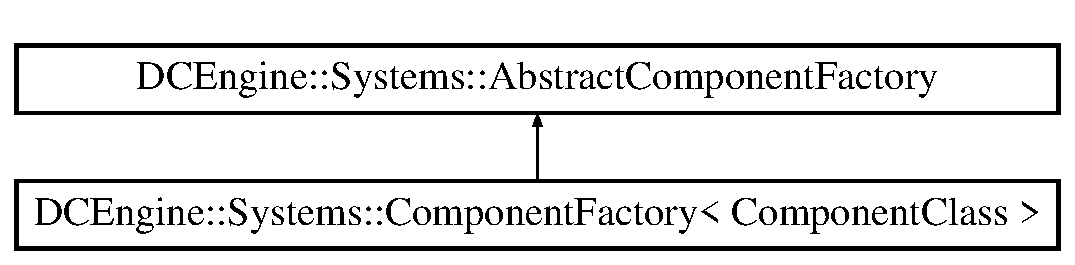
\includegraphics[height=2.000000cm]{classDCEngine_1_1Systems_1_1AbstractComponentFactory}
\end{center}
\end{figure}
\subsection*{Public Member Functions}
\begin{DoxyCompactItemize}
\item 
\hypertarget{classDCEngine_1_1Systems_1_1AbstractComponentFactory_a9276d79f8f72e74e7ffba6d576e1257a}{virtual std\-::unique\-\_\-ptr\\*
$<$ \hyperlink{classDCEngine_1_1Component}{Component} $>$ {\bfseries Construct\-Component} (\hyperlink{classDCEngine_1_1Entity}{Entity} \&owner)=0}\label{classDCEngine_1_1Systems_1_1AbstractComponentFactory_a9276d79f8f72e74e7ffba6d576e1257a}

\end{DoxyCompactItemize}


The documentation for this class was generated from the following file\-:\begin{DoxyCompactItemize}
\item 
Core/\-Systems/\-Factory/\hyperlink{ComponentFactory_8h}{Component\-Factory.\-h}\end{DoxyCompactItemize}

\hypertarget{classDCEngine_1_1Action}{\section{D\-C\-Engine\-:\-:Action Class Reference}
\label{classDCEngine_1_1Action}\index{D\-C\-Engine\-::\-Action@{D\-C\-Engine\-::\-Action}}
}
Inheritance diagram for D\-C\-Engine\-:\-:Action\-:\begin{figure}[H]
\begin{center}
\leavevmode
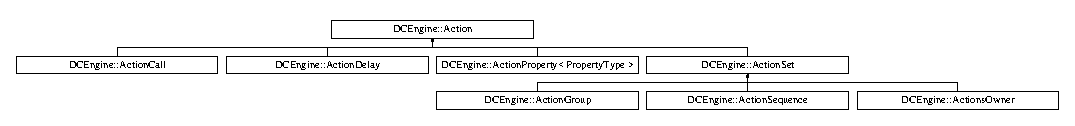
\includegraphics[height=1.249071cm]{classDCEngine_1_1Action}
\end{center}
\end{figure}
\subsection*{Public Member Functions}
\begin{DoxyCompactItemize}
\item 
\hypertarget{classDCEngine_1_1Action_a6ad5f4f266c7f34942b5d4b96a1cd138}{\hyperlink{classDCEngine_1_1Action_a6ad5f4f266c7f34942b5d4b96a1cd138}{Action} ()}\label{classDCEngine_1_1Action_a6ad5f4f266c7f34942b5d4b96a1cd138}

\begin{DoxyCompactList}\small\item\em \hyperlink{classDCEngine_1_1Action}{Action} constructor. \end{DoxyCompactList}\item 
\hypertarget{classDCEngine_1_1Action_a2dda0fc5425ccf01d83f57a90ada9136}{\hyperlink{classDCEngine_1_1Action_a2dda0fc5425ccf01d83f57a90ada9136}{$\sim$\-Action} ()}\label{classDCEngine_1_1Action_a2dda0fc5425ccf01d83f57a90ada9136}

\begin{DoxyCompactList}\small\item\em \hyperlink{classDCEngine_1_1Action}{Action} destructor. \end{DoxyCompactList}\item 
\hypertarget{classDCEngine_1_1Action_a0dd052cd4b914c78119a77fb914267e3}{virtual float {\bfseries Update} (float dt)=0}\label{classDCEngine_1_1Action_a0dd052cd4b914c78119a77fb914267e3}

\item 
\hypertarget{classDCEngine_1_1Action_a6c0213267106d544b2b39ac5d8cd9cec}{bool {\bfseries Blocking} ()}\label{classDCEngine_1_1Action_a6c0213267106d544b2b39ac5d8cd9cec}

\item 
\hypertarget{classDCEngine_1_1Action_a436718f4a14d668d81e877353dbb9e48}{bool {\bfseries Finished} ()}\label{classDCEngine_1_1Action_a436718f4a14d668d81e877353dbb9e48}

\item 
\hypertarget{classDCEngine_1_1Action_a15c1bd70492305c1f940bfe1e2d1edb3}{void {\bfseries Pause} ()}\label{classDCEngine_1_1Action_a15c1bd70492305c1f940bfe1e2d1edb3}

\item 
\hypertarget{classDCEngine_1_1Action_a908b043fa651e1b6554c3743be54a99e}{bool {\bfseries Is\-Paused} ()}\label{classDCEngine_1_1Action_a908b043fa651e1b6554c3743be54a99e}

\end{DoxyCompactItemize}
\subsection*{Protected Attributes}
\begin{DoxyCompactItemize}
\item 
\hypertarget{classDCEngine_1_1Action_adf8b42c7ff24649edc881d52446b288d}{Real {\bfseries Elapsed} = 0.\-0f}\label{classDCEngine_1_1Action_adf8b42c7ff24649edc881d52446b288d}

\item 
\hypertarget{classDCEngine_1_1Action_a1ef1f22139f834d4578d2f5848dec16b}{Real {\bfseries Duration} = 0.\-0f}\label{classDCEngine_1_1Action_a1ef1f22139f834d4578d2f5848dec16b}

\item 
\hypertarget{classDCEngine_1_1Action_aff1c14ed954cef1c419dd83cfd80814a}{bool {\bfseries Is\-Blocking} = false}\label{classDCEngine_1_1Action_aff1c14ed954cef1c419dd83cfd80814a}

\item 
\hypertarget{classDCEngine_1_1Action_a48d11994852f04abd193468ce349bae6}{bool {\bfseries Is\-Finished} = false}\label{classDCEngine_1_1Action_a48d11994852f04abd193468ce349bae6}

\item 
\hypertarget{classDCEngine_1_1Action_aa3239bf19a3b23e22fe664c913975bd1}{bool {\bfseries Paused} = false}\label{classDCEngine_1_1Action_aa3239bf19a3b23e22fe664c913975bd1}

\end{DoxyCompactItemize}


\subsection{Detailed Description}
base class from which all other actions derive from. 

The documentation for this class was generated from the following files\-:\begin{DoxyCompactItemize}
\item 
Core/\-Engine/\hyperlink{Action_8h}{Action.\-h}\item 
Core/\-Engine/\hyperlink{Actions_8cpp}{Actions.\-cpp}\end{DoxyCompactItemize}

\hypertarget{classDCEngine_1_1ActionCall}{\section{D\-C\-Engine\-:\-:Action\-Call Class Reference}
\label{classDCEngine_1_1ActionCall}\index{D\-C\-Engine\-::\-Action\-Call@{D\-C\-Engine\-::\-Action\-Call}}
}
Inheritance diagram for D\-C\-Engine\-:\-:Action\-Call\-:\begin{figure}[H]
\begin{center}
\leavevmode
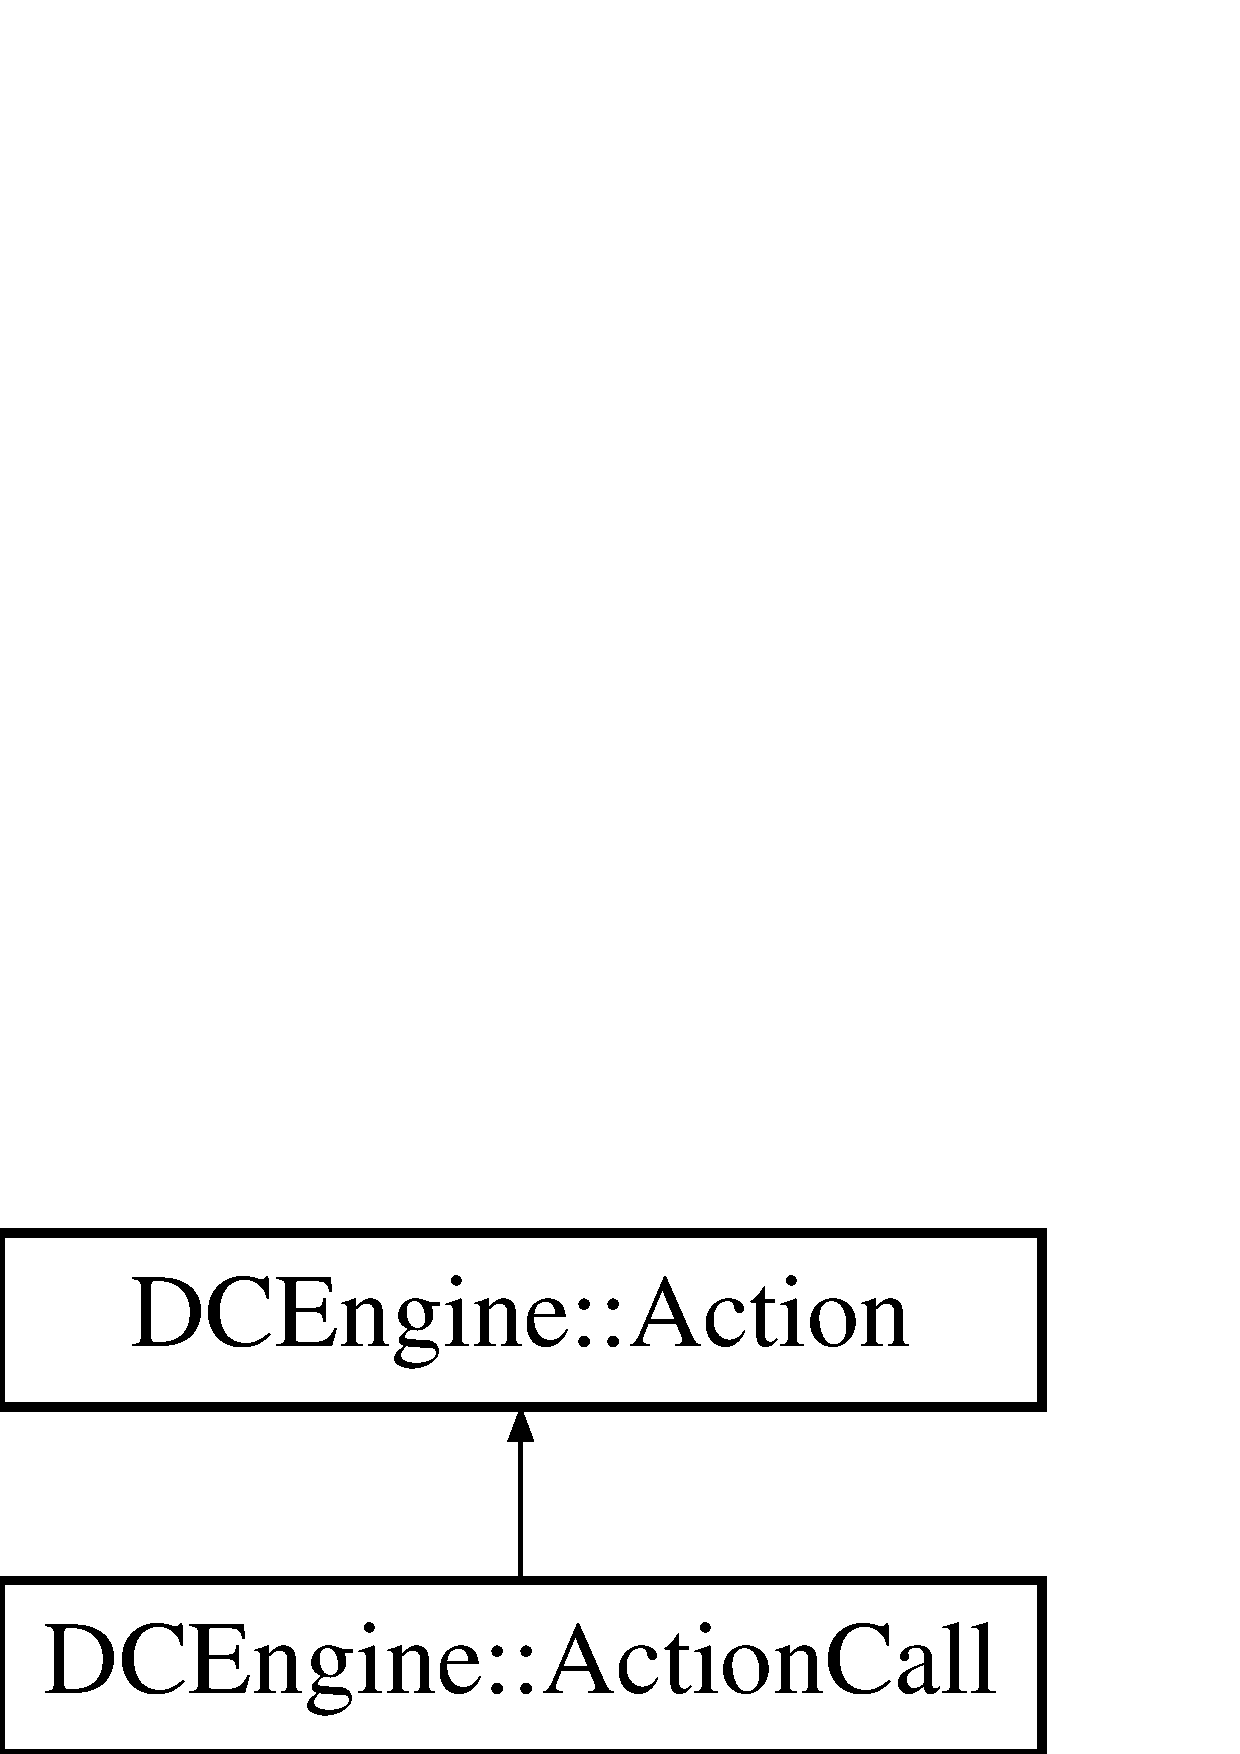
\includegraphics[height=2.000000cm]{classDCEngine_1_1ActionCall}
\end{center}
\end{figure}
\subsection*{Public Member Functions}
\begin{DoxyCompactItemize}
\item 
\hyperlink{classDCEngine_1_1ActionCall_a2cc7f5a35ff15249efb4eecca1cc17ea}{Action\-Call} (Action\-Set\-Ptr set, \hyperlink{classDCEngine_1_1Delegate}{Delegate} $\ast$func\-Ptr)
\begin{DoxyCompactList}\small\item\em \hyperlink{classDCEngine_1_1Action}{Action} Call constructor. \end{DoxyCompactList}\item 
float \hyperlink{classDCEngine_1_1ActionCall_a235459e7b9ee2094418761a3bb96dd15}{Update} (float dt)
\begin{DoxyCompactList}\small\item\em Updates this action. \end{DoxyCompactList}\end{DoxyCompactItemize}
\subsection*{Public Attributes}
\begin{DoxyCompactItemize}
\item 
\hypertarget{classDCEngine_1_1ActionCall_a47aae48f25634bd713ad99a1ab49a7ff}{\hyperlink{classDCEngine_1_1Delegate}{Delegate} $\ast$ {\bfseries Function\-Ptr}}\label{classDCEngine_1_1ActionCall_a47aae48f25634bd713ad99a1ab49a7ff}

\end{DoxyCompactItemize}
\subsection*{Additional Inherited Members}


\subsection{Constructor \& Destructor Documentation}
\hypertarget{classDCEngine_1_1ActionCall_a2cc7f5a35ff15249efb4eecca1cc17ea}{\index{D\-C\-Engine\-::\-Action\-Call@{D\-C\-Engine\-::\-Action\-Call}!Action\-Call@{Action\-Call}}
\index{Action\-Call@{Action\-Call}!DCEngine::ActionCall@{D\-C\-Engine\-::\-Action\-Call}}
\subsubsection[{Action\-Call}]{\setlength{\rightskip}{0pt plus 5cm}D\-C\-Engine\-::\-Action\-Call\-::\-Action\-Call (
\begin{DoxyParamCaption}
\item[{Action\-Set\-Ptr}]{set, }
\item[{{\bf Delegate} $\ast$}]{func\-Ptr}
\end{DoxyParamCaption}
)}}\label{classDCEngine_1_1ActionCall_a2cc7f5a35ff15249efb4eecca1cc17ea}


\hyperlink{classDCEngine_1_1Action}{Action} Call constructor. 


\begin{DoxyParams}{Parameters}
{\em sequence} & A reference to the sequence that this action will be added to. \\
\hline
{\em func\-Ptr} & A pointer to the function that will need to be called. \\
\hline
\end{DoxyParams}


\subsection{Member Function Documentation}
\hypertarget{classDCEngine_1_1ActionCall_a235459e7b9ee2094418761a3bb96dd15}{\index{D\-C\-Engine\-::\-Action\-Call@{D\-C\-Engine\-::\-Action\-Call}!Update@{Update}}
\index{Update@{Update}!DCEngine::ActionCall@{D\-C\-Engine\-::\-Action\-Call}}
\subsubsection[{Update}]{\setlength{\rightskip}{0pt plus 5cm}float D\-C\-Engine\-::\-Action\-Call\-::\-Update (
\begin{DoxyParamCaption}
\item[{float}]{dt}
\end{DoxyParamCaption}
)\hspace{0.3cm}{\ttfamily [virtual]}}}\label{classDCEngine_1_1ActionCall_a235459e7b9ee2094418761a3bb96dd15}


Updates this action. 


\begin{DoxyParams}{Parameters}
{\em dt} & \hyperlink{classThe}{The} time slice given. \\
\hline
\end{DoxyParams}
\begin{DoxyReturn}{Returns}
How muc time was consumed. 
\end{DoxyReturn}


Implements \hyperlink{classDCEngine_1_1Action}{D\-C\-Engine\-::\-Action}.



The documentation for this class was generated from the following files\-:\begin{DoxyCompactItemize}
\item 
Core/\-Engine/\hyperlink{Action_8h}{Action.\-h}\item 
Core/\-Engine/\hyperlink{ActionCall_8cpp}{Action\-Call.\-cpp}\end{DoxyCompactItemize}

\hypertarget{classDCEngine_1_1ActionDelay}{\section{D\-C\-Engine\-:\-:Action\-Delay Class Reference}
\label{classDCEngine_1_1ActionDelay}\index{D\-C\-Engine\-::\-Action\-Delay@{D\-C\-Engine\-::\-Action\-Delay}}
}
Inheritance diagram for D\-C\-Engine\-:\-:Action\-Delay\-:\begin{figure}[H]
\begin{center}
\leavevmode
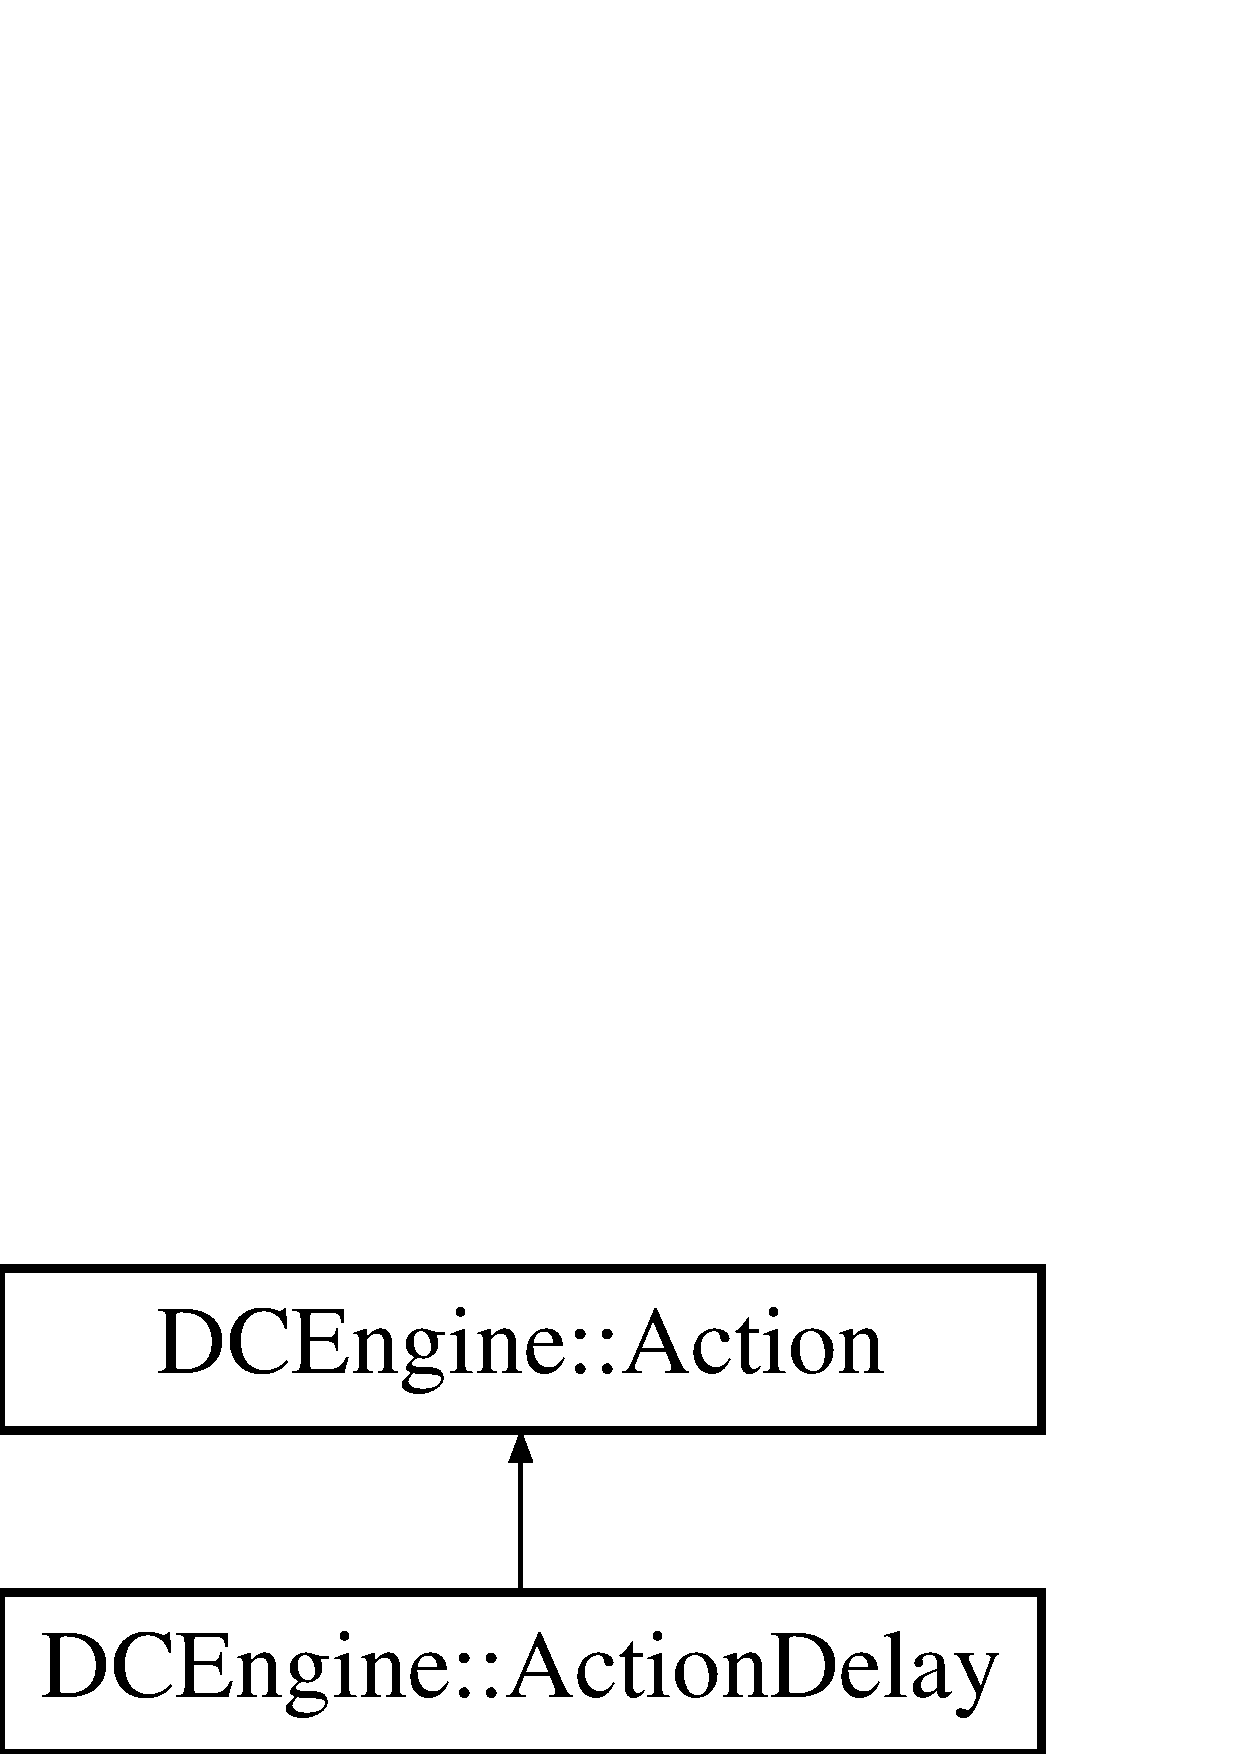
\includegraphics[height=2.000000cm]{classDCEngine_1_1ActionDelay}
\end{center}
\end{figure}
\subsection*{Public Member Functions}
\begin{DoxyCompactItemize}
\item 
\hyperlink{classDCEngine_1_1ActionDelay_a6105b09652c8a0402e386ac752a8463c}{Action\-Delay} (Action\-Set\-Ptr set, Real duration)
\begin{DoxyCompactList}\small\item\em \hyperlink{classDCEngine_1_1ActionDelay}{Action\-Delay} constructor. \end{DoxyCompactList}\item 
float \hyperlink{classDCEngine_1_1ActionDelay_af35735d6290b9d1ac8cb3e7f0a334c84}{Update} (float dt)
\begin{DoxyCompactList}\small\item\em Updates this action. \end{DoxyCompactList}\end{DoxyCompactItemize}
\subsection*{Additional Inherited Members}


\subsection{Constructor \& Destructor Documentation}
\hypertarget{classDCEngine_1_1ActionDelay_a6105b09652c8a0402e386ac752a8463c}{\index{D\-C\-Engine\-::\-Action\-Delay@{D\-C\-Engine\-::\-Action\-Delay}!Action\-Delay@{Action\-Delay}}
\index{Action\-Delay@{Action\-Delay}!DCEngine::ActionDelay@{D\-C\-Engine\-::\-Action\-Delay}}
\subsubsection[{Action\-Delay}]{\setlength{\rightskip}{0pt plus 5cm}D\-C\-Engine\-::\-Action\-Delay\-::\-Action\-Delay (
\begin{DoxyParamCaption}
\item[{Action\-Set\-Ptr}]{set, }
\item[{Real}]{duration}
\end{DoxyParamCaption}
)}}\label{classDCEngine_1_1ActionDelay_a6105b09652c8a0402e386ac752a8463c}


\hyperlink{classDCEngine_1_1ActionDelay}{Action\-Delay} constructor. 


\begin{DoxyParams}{Parameters}
{\em sequence} & \hyperlink{classA}{A} reference to the sequence of actions this action belongs to. \\
\hline
{\em dt} & \hyperlink{classThe}{The} duration for this delay action. \\
\hline
\end{DoxyParams}


\subsection{Member Function Documentation}
\hypertarget{classDCEngine_1_1ActionDelay_af35735d6290b9d1ac8cb3e7f0a334c84}{\index{D\-C\-Engine\-::\-Action\-Delay@{D\-C\-Engine\-::\-Action\-Delay}!Update@{Update}}
\index{Update@{Update}!DCEngine::ActionDelay@{D\-C\-Engine\-::\-Action\-Delay}}
\subsubsection[{Update}]{\setlength{\rightskip}{0pt plus 5cm}float D\-C\-Engine\-::\-Action\-Delay\-::\-Update (
\begin{DoxyParamCaption}
\item[{float}]{dt}
\end{DoxyParamCaption}
)\hspace{0.3cm}{\ttfamily [virtual]}}}\label{classDCEngine_1_1ActionDelay_af35735d6290b9d1ac8cb3e7f0a334c84}


Updates this action. 


\begin{DoxyParams}{Parameters}
{\em dt} & \hyperlink{classThe}{The} time slice given. \\
\hline
\end{DoxyParams}
\begin{DoxyReturn}{Returns}
How much time was consumed during this action 
\end{DoxyReturn}


Implements \hyperlink{classDCEngine_1_1Action}{D\-C\-Engine\-::\-Action}.



The documentation for this class was generated from the following files\-:\begin{DoxyCompactItemize}
\item 
Core/\-Engine/\hyperlink{Action_8h}{Action.\-h}\item 
Core/\-Engine/\hyperlink{ActionDelay_8cpp}{Action\-Delay.\-cpp}\end{DoxyCompactItemize}

\hypertarget{classDCEngine_1_1ActionGroup}{\section{D\-C\-Engine\-:\-:Action\-Group Class Reference}
\label{classDCEngine_1_1ActionGroup}\index{D\-C\-Engine\-::\-Action\-Group@{D\-C\-Engine\-::\-Action\-Group}}
}
Inheritance diagram for D\-C\-Engine\-:\-:Action\-Group\-:\begin{figure}[H]
\begin{center}
\leavevmode
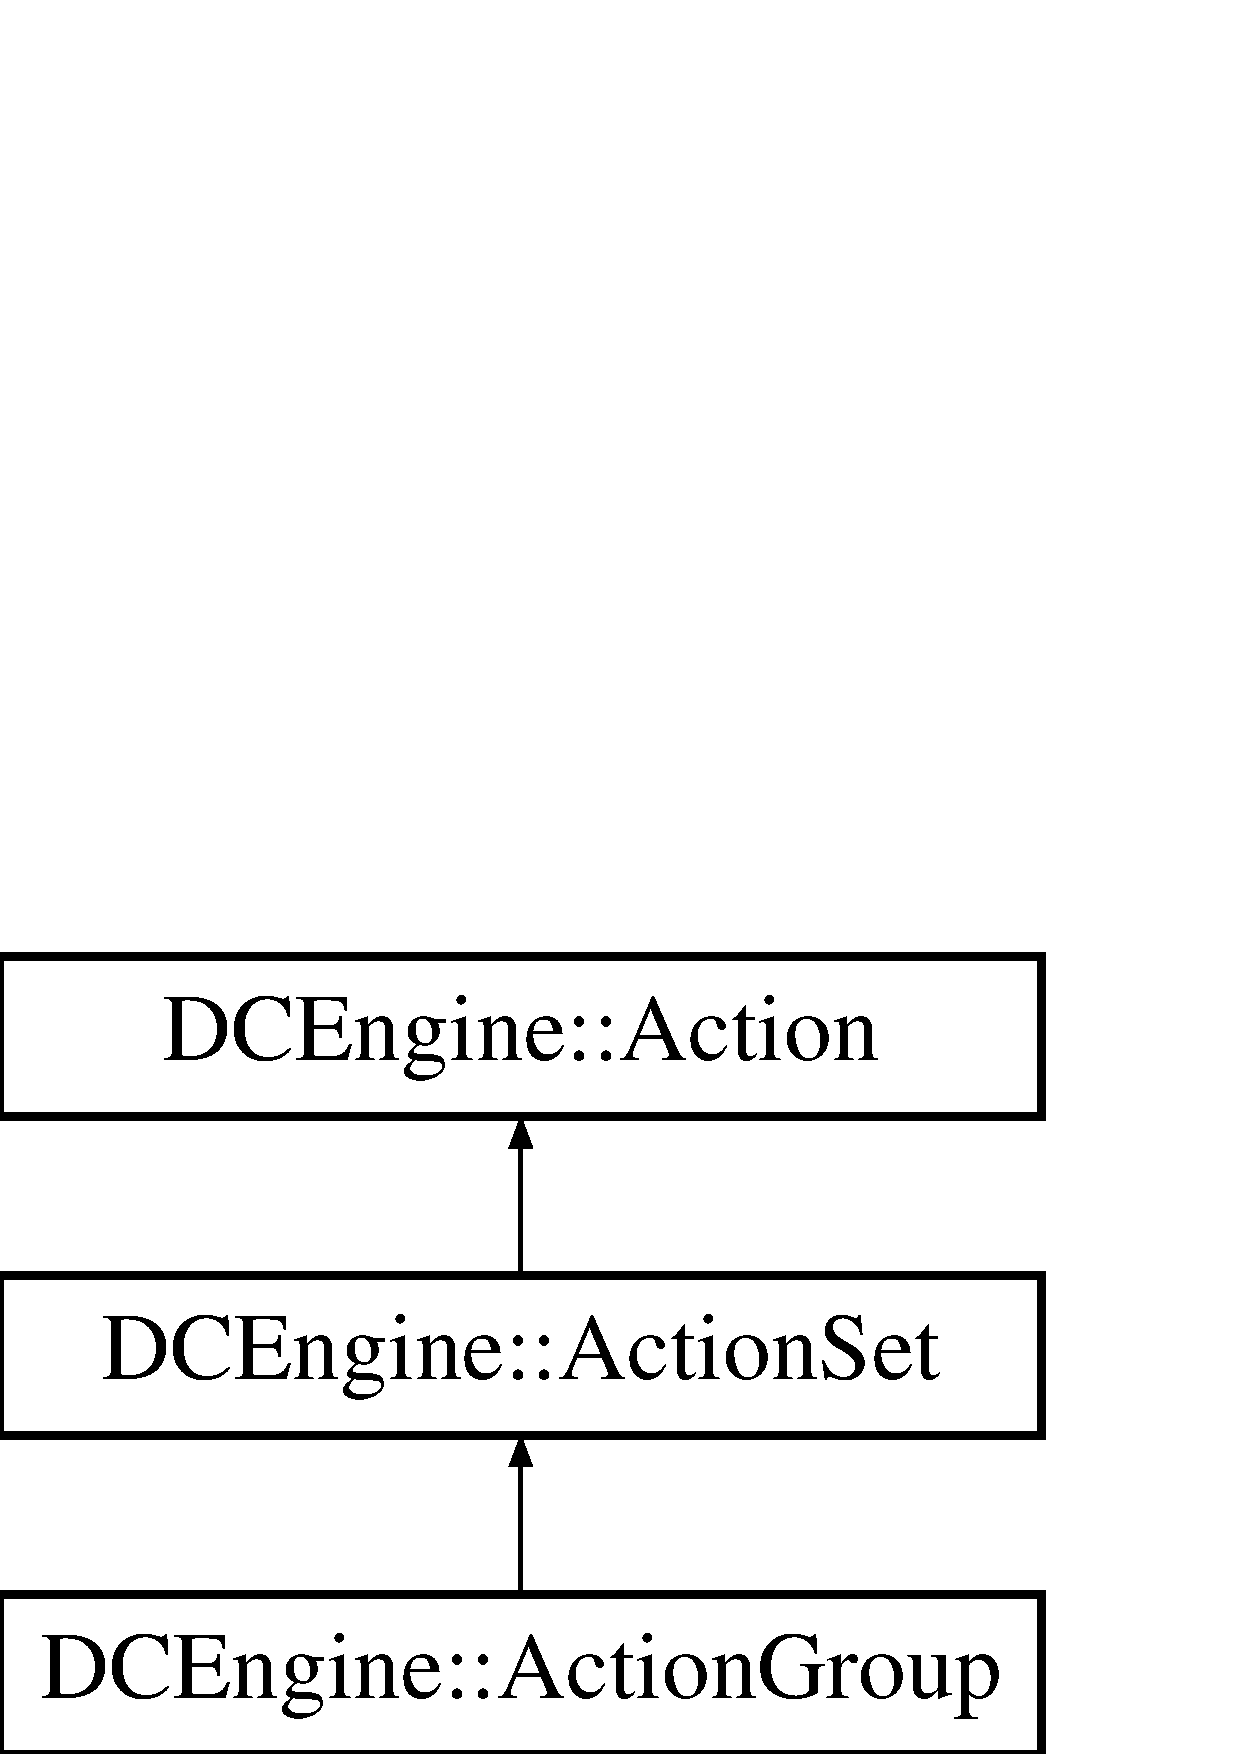
\includegraphics[height=3.000000cm]{classDCEngine_1_1ActionGroup}
\end{center}
\end{figure}
\subsection*{Public Member Functions}
\begin{DoxyCompactItemize}
\item 
float \hyperlink{classDCEngine_1_1ActionGroup_acccb315e591d55fc71f1475471a8cc7a}{Update} (float dt)
\begin{DoxyCompactList}\small\item\em Updates an \hyperlink{classDCEngine_1_1ActionGroup}{Action\-Group}, by updating the actions in the group in parallel. \end{DoxyCompactList}\end{DoxyCompactItemize}
\subsection*{Additional Inherited Members}


\subsection{Member Function Documentation}
\hypertarget{classDCEngine_1_1ActionGroup_acccb315e591d55fc71f1475471a8cc7a}{\index{D\-C\-Engine\-::\-Action\-Group@{D\-C\-Engine\-::\-Action\-Group}!Update@{Update}}
\index{Update@{Update}!DCEngine::ActionGroup@{D\-C\-Engine\-::\-Action\-Group}}
\subsubsection[{Update}]{\setlength{\rightskip}{0pt plus 5cm}float D\-C\-Engine\-::\-Action\-Group\-::\-Update (
\begin{DoxyParamCaption}
\item[{float}]{dt}
\end{DoxyParamCaption}
)\hspace{0.3cm}{\ttfamily [virtual]}}}\label{classDCEngine_1_1ActionGroup_acccb315e591d55fc71f1475471a8cc7a}


Updates an \hyperlink{classDCEngine_1_1ActionGroup}{Action\-Group}, by updating the actions in the group in parallel. 


\begin{DoxyParams}{Parameters}
{\em dt} & \hyperlink{classThe}{The} time to be updated. \\
\hline
\end{DoxyParams}
\begin{DoxyReturn}{Returns}
How much time was consumed while updating. 
\end{DoxyReturn}


Implements \hyperlink{classDCEngine_1_1ActionSet}{D\-C\-Engine\-::\-Action\-Set}.



The documentation for this class was generated from the following files\-:\begin{DoxyCompactItemize}
\item 
Core/\-Engine/\hyperlink{Action_8h}{Action.\-h}\item 
Core/\-Engine/Action\-Set.\-cpp\end{DoxyCompactItemize}

\hypertarget{classDCEngine_1_1ActionProperty}{\section{D\-C\-Engine\-:\-:Action\-Property$<$ Property\-Type $>$ Class Template Reference}
\label{classDCEngine_1_1ActionProperty}\index{D\-C\-Engine\-::\-Action\-Property$<$ Property\-Type $>$@{D\-C\-Engine\-::\-Action\-Property$<$ Property\-Type $>$}}
}
Inheritance diagram for D\-C\-Engine\-:\-:Action\-Property$<$ Property\-Type $>$\-:\begin{figure}[H]
\begin{center}
\leavevmode
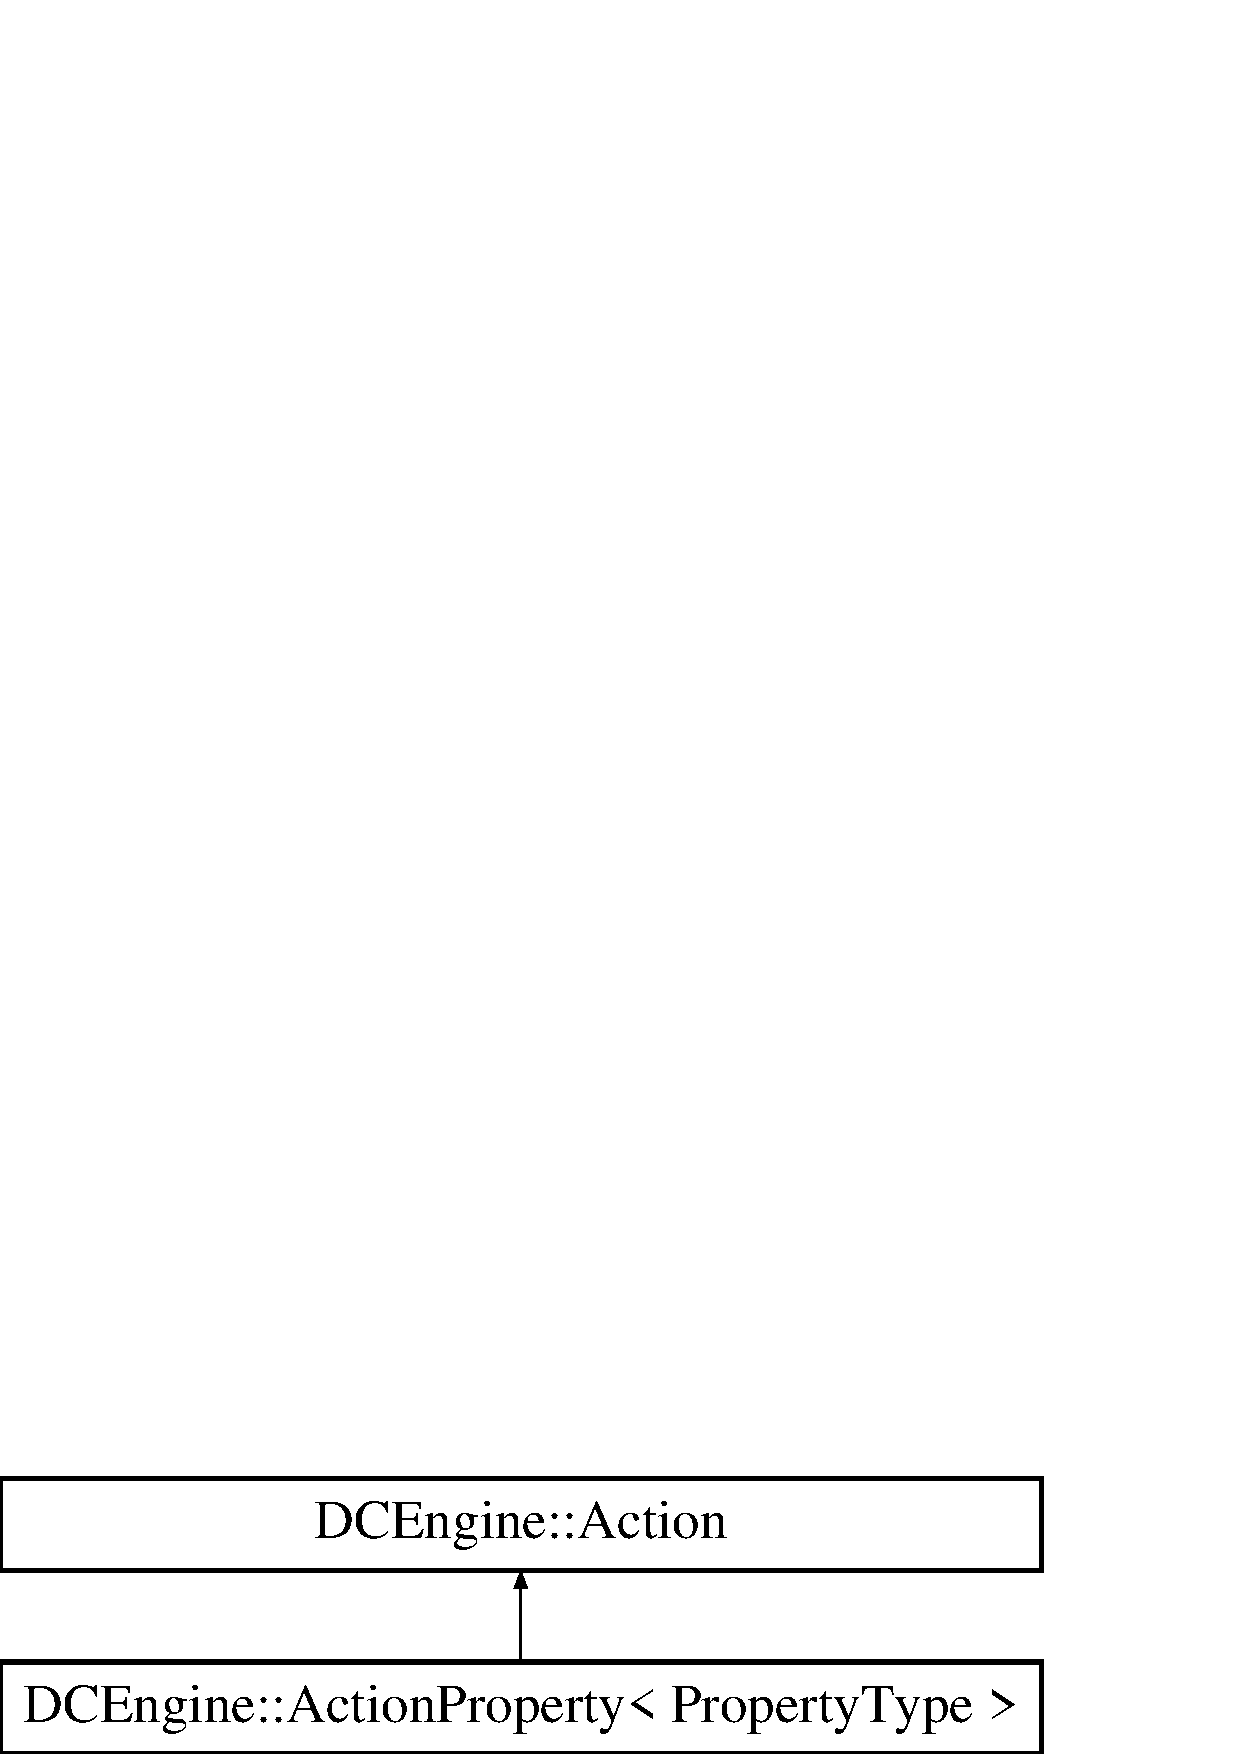
\includegraphics[height=2.000000cm]{classDCEngine_1_1ActionProperty}
\end{center}
\end{figure}
\subsection*{Public Member Functions}
\begin{DoxyCompactItemize}
\item 
\hypertarget{classDCEngine_1_1ActionProperty_a5357b40640fb1fe77499eb6b5986b52b}{{\bfseries Action\-Property} (\hyperlink{classDCEngine_1_1ActionSet}{Action\-Set} \&sequence, Property\-Type \&prop, Real duration, Ease ease)}\label{classDCEngine_1_1ActionProperty_a5357b40640fb1fe77499eb6b5986b52b}

\item 
float \hyperlink{classDCEngine_1_1ActionProperty_aca45929048463086d5b05bb4287ab4f6}{Update} (float dt)
\begin{DoxyCompactList}\small\item\em \hyperlink{classDCEngine_1_1ActionProperty}{Action\-Property} constructor. \end{DoxyCompactList}\end{DoxyCompactItemize}
\subsection*{Additional Inherited Members}


\subsection{Member Function Documentation}
\hypertarget{classDCEngine_1_1ActionProperty_aca45929048463086d5b05bb4287ab4f6}{\index{D\-C\-Engine\-::\-Action\-Property@{D\-C\-Engine\-::\-Action\-Property}!Update@{Update}}
\index{Update@{Update}!DCEngine::ActionProperty@{D\-C\-Engine\-::\-Action\-Property}}
\subsubsection[{Update}]{\setlength{\rightskip}{0pt plus 5cm}template$<$typename Property\-Type $>$ float {\bf D\-C\-Engine\-::\-Action\-Property}$<$ Property\-Type $>$\-::Update (
\begin{DoxyParamCaption}
\item[{float}]{dt}
\end{DoxyParamCaption}
)\hspace{0.3cm}{\ttfamily [inline]}, {\ttfamily [virtual]}}}\label{classDCEngine_1_1ActionProperty_aca45929048463086d5b05bb4287ab4f6}


\hyperlink{classDCEngine_1_1ActionProperty}{Action\-Property} constructor. 


\begin{DoxyParams}{Parameters}
{\em Property\-Type} & \hyperlink{classThe}{The} P\-O\-D or class type of the property; \\
\hline
{\em set} & A reference to the set this property is part of. \\
\hline
{\em property} & A reference to the property to be modified. \\
\hline
{\em duration} & How long this property runs for. \\
\hline
{\em ease} & What ease this property uses to calculate the interpolation.\\
\hline
\end{DoxyParams}
Updates the property. 
\begin{DoxyParams}{Parameters}
{\em dt} & \hyperlink{classThe}{The} time slice given. \\
\hline
\end{DoxyParams}


Implements \hyperlink{classDCEngine_1_1Action}{D\-C\-Engine\-::\-Action}.



The documentation for this class was generated from the following file\-:\begin{DoxyCompactItemize}
\item 
Core/\-Engine/\hyperlink{Action_8h}{Action.\-h}\end{DoxyCompactItemize}

\hypertarget{classDCEngine_1_1Actions}{\section{D\-C\-Engine\-:\-:Actions Class Reference}
\label{classDCEngine_1_1Actions}\index{D\-C\-Engine\-::\-Actions@{D\-C\-Engine\-::\-Actions}}
}
\subsection*{Static Public Member Functions}
\begin{DoxyCompactItemize}
\item 
static Action\-Set\-Ptr \hyperlink{classDCEngine_1_1Actions_a9c1cfb84ef8a34a9e40824c21d09bf11}{Sequence} (\hyperlink{classDCEngine_1_1ActionSet}{Action\-Set} \&owner)
\begin{DoxyCompactList}\small\item\em Creates an action sequence. \end{DoxyCompactList}\item 
static Action\-Set\-Ptr \hyperlink{classDCEngine_1_1Actions_a45126cc19656693474c2c3ed90bd4ed1}{Group} (\hyperlink{classDCEngine_1_1ActionSet}{Action\-Set} \&owner)
\begin{DoxyCompactList}\small\item\em Creates an action sequence. \end{DoxyCompactList}\item 
static void \hyperlink{classDCEngine_1_1Actions_a8c098c5645c80d97234ae97299b3d426}{Call} (Action\-Set\-Ptr set, void $\ast$fn)
\begin{DoxyCompactList}\small\item\em Creates an \hyperlink{classDCEngine_1_1ActionCall}{Action\-Call}. \end{DoxyCompactList}\item 
static void \hyperlink{classDCEngine_1_1Actions_a6c4528212320eba1bc7e13417ce458b2}{Delay} (Action\-Set\-Ptr set, Real duration)
\begin{DoxyCompactList}\small\item\em Creates an \hyperlink{classDCEngine_1_1ActionDelay}{Action\-Delay}. \end{DoxyCompactList}\item 
\hypertarget{classDCEngine_1_1Actions_aa94bbf255d175be5c62d44424daf7d47}{{\footnotesize template$<$typename Property $>$ }\\static void {\bfseries Property} (\hyperlink{classDCEngine_1_1ActionSequence}{Action\-Sequence} \&seq, Property \&prty, Property val, Real duration, Ease ease)}\label{classDCEngine_1_1Actions_aa94bbf255d175be5c62d44424daf7d47}

\end{DoxyCompactItemize}


\subsection{Member Function Documentation}
\hypertarget{classDCEngine_1_1Actions_a8c098c5645c80d97234ae97299b3d426}{\index{D\-C\-Engine\-::\-Actions@{D\-C\-Engine\-::\-Actions}!Call@{Call}}
\index{Call@{Call}!DCEngine::Actions@{D\-C\-Engine\-::\-Actions}}
\subsubsection[{Call}]{\setlength{\rightskip}{0pt plus 5cm}void D\-C\-Engine\-::\-Actions\-::\-Call (
\begin{DoxyParamCaption}
\item[{Action\-Set\-Ptr}]{set, }
\item[{void $\ast$}]{fn}
\end{DoxyParamCaption}
)\hspace{0.3cm}{\ttfamily [static]}}}\label{classDCEngine_1_1Actions_a8c098c5645c80d97234ae97299b3d426}


Creates an \hyperlink{classDCEngine_1_1ActionCall}{Action\-Call}. 


\begin{DoxyParams}{Parameters}
{\em set} & A reference to the \hyperlink{classDCEngine_1_1ActionSet}{Action\-Set} that this action belongs to. \\
\hline
{\em fn} & A reference to the function that will be added. \\
\hline
\end{DoxyParams}
\hypertarget{classDCEngine_1_1Actions_a6c4528212320eba1bc7e13417ce458b2}{\index{D\-C\-Engine\-::\-Actions@{D\-C\-Engine\-::\-Actions}!Delay@{Delay}}
\index{Delay@{Delay}!DCEngine::Actions@{D\-C\-Engine\-::\-Actions}}
\subsubsection[{Delay}]{\setlength{\rightskip}{0pt plus 5cm}void D\-C\-Engine\-::\-Actions\-::\-Delay (
\begin{DoxyParamCaption}
\item[{Action\-Set\-Ptr}]{set, }
\item[{Real}]{duration}
\end{DoxyParamCaption}
)\hspace{0.3cm}{\ttfamily [static]}}}\label{classDCEngine_1_1Actions_a6c4528212320eba1bc7e13417ce458b2}


Creates an \hyperlink{classDCEngine_1_1ActionDelay}{Action\-Delay}. 


\begin{DoxyParams}{Parameters}
{\em set} & A reference to the \hyperlink{classDCEngine_1_1ActionSet}{Action\-Set} that this action belongs to. \\
\hline
{\em duration} & How long should the delay run for. \\
\hline
\end{DoxyParams}
\hypertarget{classDCEngine_1_1Actions_a45126cc19656693474c2c3ed90bd4ed1}{\index{D\-C\-Engine\-::\-Actions@{D\-C\-Engine\-::\-Actions}!Group@{Group}}
\index{Group@{Group}!DCEngine::Actions@{D\-C\-Engine\-::\-Actions}}
\subsubsection[{Group}]{\setlength{\rightskip}{0pt plus 5cm}Action\-Set\-Ptr D\-C\-Engine\-::\-Actions\-::\-Group (
\begin{DoxyParamCaption}
\item[{{\bf Action\-Set} \&}]{owner}
\end{DoxyParamCaption}
)\hspace{0.3cm}{\ttfamily [static]}}}\label{classDCEngine_1_1Actions_a45126cc19656693474c2c3ed90bd4ed1}


Creates an action sequence. 


\begin{DoxyParams}{Parameters}
{\em owner} & A reference to the owner of this action sequence. \\
\hline
\end{DoxyParams}
\hypertarget{classDCEngine_1_1Actions_a9c1cfb84ef8a34a9e40824c21d09bf11}{\index{D\-C\-Engine\-::\-Actions@{D\-C\-Engine\-::\-Actions}!Sequence@{Sequence}}
\index{Sequence@{Sequence}!DCEngine::Actions@{D\-C\-Engine\-::\-Actions}}
\subsubsection[{Sequence}]{\setlength{\rightskip}{0pt plus 5cm}Action\-Set\-Ptr D\-C\-Engine\-::\-Actions\-::\-Sequence (
\begin{DoxyParamCaption}
\item[{{\bf Action\-Set} \&}]{owner}
\end{DoxyParamCaption}
)\hspace{0.3cm}{\ttfamily [static]}}}\label{classDCEngine_1_1Actions_a9c1cfb84ef8a34a9e40824c21d09bf11}


Creates an action sequence. 


\begin{DoxyParams}{Parameters}
{\em owner} & A reference to the owner of this action sequence. \\
\hline
\end{DoxyParams}


The documentation for this class was generated from the following files\-:\begin{DoxyCompactItemize}
\item 
Core/\-Engine/\hyperlink{Action_8h}{Action.\-h}\item 
Core/\-Engine/\hyperlink{Actions_8cpp}{Actions.\-cpp}\end{DoxyCompactItemize}

\hypertarget{classDCEngine_1_1ActionSequence}{\section{D\-C\-Engine\-:\-:Action\-Sequence Class Reference}
\label{classDCEngine_1_1ActionSequence}\index{D\-C\-Engine\-::\-Action\-Sequence@{D\-C\-Engine\-::\-Action\-Sequence}}
}
Inheritance diagram for D\-C\-Engine\-:\-:Action\-Sequence\-:\begin{figure}[H]
\begin{center}
\leavevmode
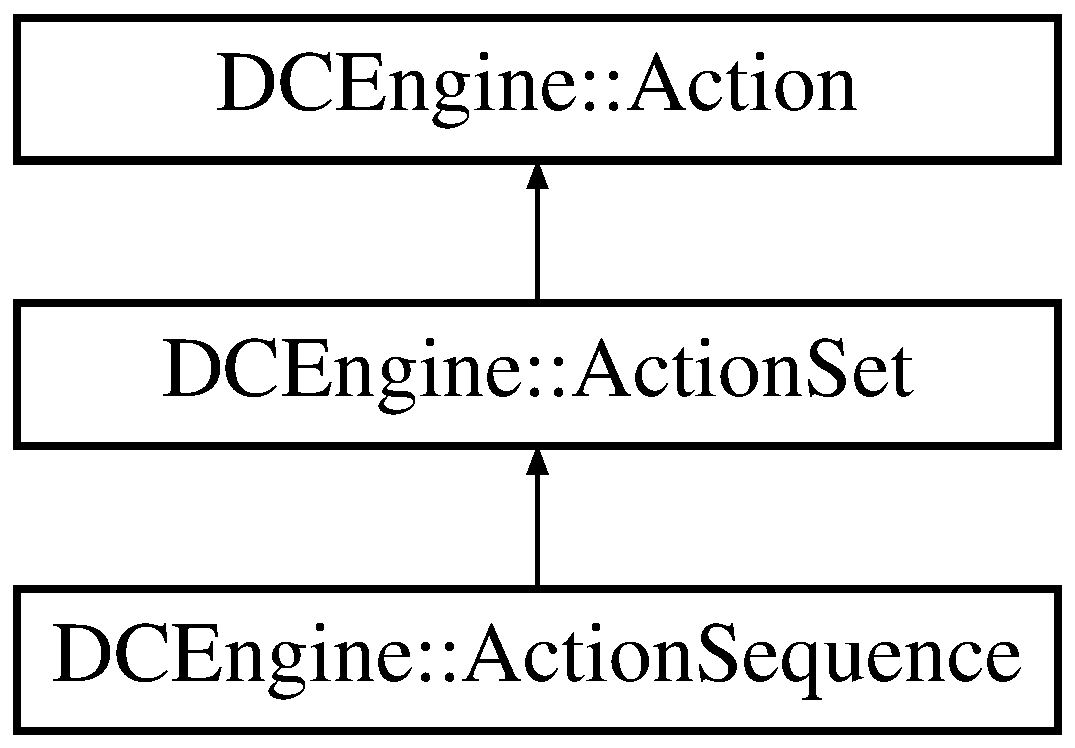
\includegraphics[height=3.000000cm]{classDCEngine_1_1ActionSequence}
\end{center}
\end{figure}
\subsection*{Public Member Functions}
\begin{DoxyCompactItemize}
\item 
float \hyperlink{classDCEngine_1_1ActionSequence_ad193db69891cf3a18bce895a19540b6e}{Update} (float dt)
\begin{DoxyCompactList}\small\item\em Updates an \hyperlink{classDCEngine_1_1ActionSequence}{Action\-Sequence}, by updating the actions in the sequence sequentially. \end{DoxyCompactList}\end{DoxyCompactItemize}
\subsection*{Additional Inherited Members}


\subsection{Member Function Documentation}
\hypertarget{classDCEngine_1_1ActionSequence_ad193db69891cf3a18bce895a19540b6e}{\index{D\-C\-Engine\-::\-Action\-Sequence@{D\-C\-Engine\-::\-Action\-Sequence}!Update@{Update}}
\index{Update@{Update}!DCEngine::ActionSequence@{D\-C\-Engine\-::\-Action\-Sequence}}
\subsubsection[{Update}]{\setlength{\rightskip}{0pt plus 5cm}float D\-C\-Engine\-::\-Action\-Sequence\-::\-Update (
\begin{DoxyParamCaption}
\item[{float}]{dt}
\end{DoxyParamCaption}
)\hspace{0.3cm}{\ttfamily [virtual]}}}\label{classDCEngine_1_1ActionSequence_ad193db69891cf3a18bce895a19540b6e}


Updates an \hyperlink{classDCEngine_1_1ActionSequence}{Action\-Sequence}, by updating the actions in the sequence sequentially. 


\begin{DoxyParams}{Parameters}
{\em dt} & \hyperlink{classThe}{The} time to be updated. \\
\hline
\end{DoxyParams}
\begin{DoxyReturn}{Returns}
How much time was consumed while updating. 
\end{DoxyReturn}


Implements \hyperlink{classDCEngine_1_1ActionSet}{D\-C\-Engine\-::\-Action\-Set}.



The documentation for this class was generated from the following files\-:\begin{DoxyCompactItemize}
\item 
Core/\-Engine/\hyperlink{Action_8h}{Action.\-h}\item 
Core/\-Engine/Action\-Set.\-cpp\end{DoxyCompactItemize}

\hypertarget{classDCEngine_1_1ActionSet}{\section{D\-C\-Engine\-:\-:Action\-Set Class Reference}
\label{classDCEngine_1_1ActionSet}\index{D\-C\-Engine\-::\-Action\-Set@{D\-C\-Engine\-::\-Action\-Set}}
}
Inheritance diagram for D\-C\-Engine\-:\-:Action\-Set\-:\begin{figure}[H]
\begin{center}
\leavevmode
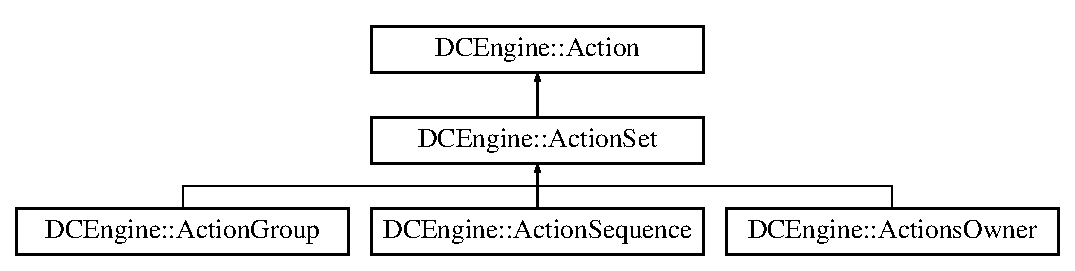
\includegraphics[height=3.000000cm]{classDCEngine_1_1ActionSet}
\end{center}
\end{figure}
\subsection*{Public Member Functions}
\begin{DoxyCompactItemize}
\item 
virtual void \hyperlink{classDCEngine_1_1ActionSet_a5e63f68a0161b788d218ca5f5bcbe0bd}{Add} (Action\-Set\-Ptr set)
\begin{DoxyCompactList}\small\item\em Adds an \hyperlink{classDCEngine_1_1ActionSet}{Action\-Set} to this set, as a child set. \end{DoxyCompactList}\item 
virtual void \hyperlink{classDCEngine_1_1ActionSet_ad8b8b1480f6f99da48b5b5d4188eaac9}{Add} (Action\-Ptr action)
\begin{DoxyCompactList}\small\item\em Adds an \hyperlink{classDCEngine_1_1Action}{Action} to this set, as one of its active actions. \end{DoxyCompactList}\item 
\hypertarget{classDCEngine_1_1ActionSet_aa231dcf08d43ad1ebad7aaa7fe1b420f}{virtual float {\bfseries Update} (float dt)=0}\label{classDCEngine_1_1ActionSet_aa231dcf08d43ad1ebad7aaa7fe1b420f}

\item 
\hypertarget{classDCEngine_1_1ActionSet_afa7f0f31e3d469c0696cc74aa1e534f4}{virtual bool \hyperlink{classDCEngine_1_1ActionSet_afa7f0f31e3d469c0696cc74aa1e534f4}{Validate} ()}\label{classDCEngine_1_1ActionSet_afa7f0f31e3d469c0696cc74aa1e534f4}

\begin{DoxyCompactList}\small\item\em Checks whether there are any remaining actions in the \hyperlink{classDCEngine_1_1ActionSet}{Action\-Set}. If there's no more remaining, the set is done. \end{DoxyCompactList}\end{DoxyCompactItemize}
\subsection*{Protected Member Functions}
\begin{DoxyCompactItemize}
\item 
\hypertarget{classDCEngine_1_1ActionSet_ad098f7230dc65f29c2a3ec2f91d0ea64}{void \hyperlink{classDCEngine_1_1ActionSet_ad098f7230dc65f29c2a3ec2f91d0ea64}{Clear} ()}\label{classDCEngine_1_1ActionSet_ad098f7230dc65f29c2a3ec2f91d0ea64}

\begin{DoxyCompactList}\small\item\em Clears all inactive actions. \end{DoxyCompactList}\end{DoxyCompactItemize}
\subsection*{Protected Attributes}
\begin{DoxyCompactItemize}
\item 
\hypertarget{classDCEngine_1_1ActionSet_ac12fecfc720a5438329bcee88cbf1f7d}{std\-::vector$<$ Action\-Ptr $>$ {\bfseries Active\-Actions}}\label{classDCEngine_1_1ActionSet_ac12fecfc720a5438329bcee88cbf1f7d}

\item 
\hypertarget{classDCEngine_1_1ActionSet_a5e6fdd39967bc7d4a81c0cbdaccf466c}{std\-::vector$<$ Action\-Ptr $>$ {\bfseries Inactive\-Actions}}\label{classDCEngine_1_1ActionSet_a5e6fdd39967bc7d4a81c0cbdaccf466c}

\end{DoxyCompactItemize}


\subsection{Member Function Documentation}
\hypertarget{classDCEngine_1_1ActionSet_a5e63f68a0161b788d218ca5f5bcbe0bd}{\index{D\-C\-Engine\-::\-Action\-Set@{D\-C\-Engine\-::\-Action\-Set}!Add@{Add}}
\index{Add@{Add}!DCEngine::ActionSet@{D\-C\-Engine\-::\-Action\-Set}}
\subsubsection[{Add}]{\setlength{\rightskip}{0pt plus 5cm}void D\-C\-Engine\-::\-Action\-Set\-::\-Add (
\begin{DoxyParamCaption}
\item[{Action\-Set\-Ptr}]{set}
\end{DoxyParamCaption}
)\hspace{0.3cm}{\ttfamily [virtual]}}}\label{classDCEngine_1_1ActionSet_a5e63f68a0161b788d218ca5f5bcbe0bd}


Adds an \hyperlink{classDCEngine_1_1ActionSet}{Action\-Set} to this set, as a child set. 


\begin{DoxyParams}{Parameters}
{\em set} & A reference to the child set. \\
\hline
\end{DoxyParams}
\hypertarget{classDCEngine_1_1ActionSet_ad8b8b1480f6f99da48b5b5d4188eaac9}{\index{D\-C\-Engine\-::\-Action\-Set@{D\-C\-Engine\-::\-Action\-Set}!Add@{Add}}
\index{Add@{Add}!DCEngine::ActionSet@{D\-C\-Engine\-::\-Action\-Set}}
\subsubsection[{Add}]{\setlength{\rightskip}{0pt plus 5cm}void D\-C\-Engine\-::\-Action\-Set\-::\-Add (
\begin{DoxyParamCaption}
\item[{Action\-Ptr}]{action}
\end{DoxyParamCaption}
)\hspace{0.3cm}{\ttfamily [virtual]}}}\label{classDCEngine_1_1ActionSet_ad8b8b1480f6f99da48b5b5d4188eaac9}


Adds an \hyperlink{classDCEngine_1_1Action}{Action} to this set, as one of its active actions. 


\begin{DoxyParams}{Parameters}
{\em action} & A pointer to the other action. \\
\hline
\end{DoxyParams}


The documentation for this class was generated from the following files\-:\begin{DoxyCompactItemize}
\item 
Core/\-Engine/\hyperlink{Action_8h}{Action.\-h}\item 
Core/\-Engine/Action\-Set.\-cpp\end{DoxyCompactItemize}

\hypertarget{classDCEngine_1_1ActionsOwner}{\section{D\-C\-Engine\-:\-:Actions\-Owner Class Reference}
\label{classDCEngine_1_1ActionsOwner}\index{D\-C\-Engine\-::\-Actions\-Owner@{D\-C\-Engine\-::\-Actions\-Owner}}
}
Inheritance diagram for D\-C\-Engine\-:\-:Actions\-Owner\-:\begin{figure}[H]
\begin{center}
\leavevmode
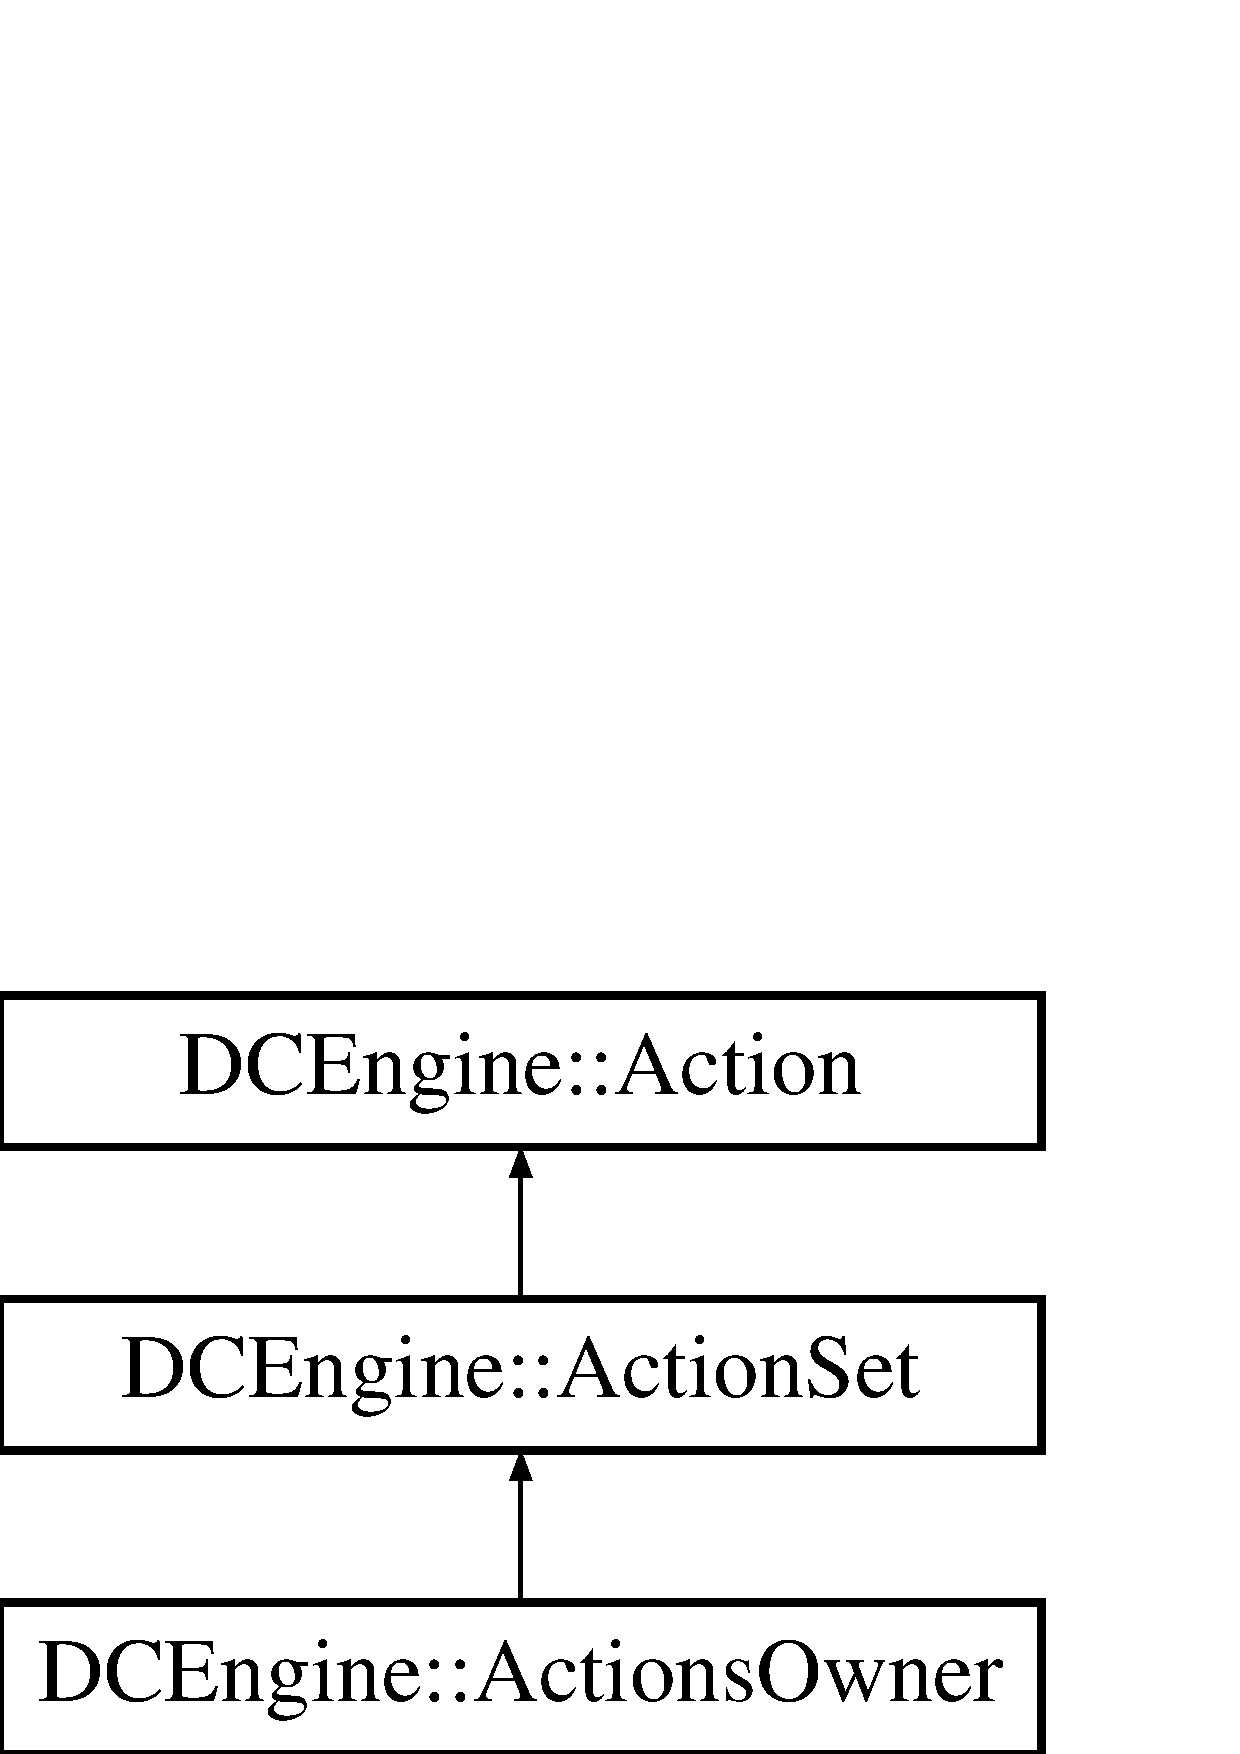
\includegraphics[height=3.000000cm]{classDCEngine_1_1ActionsOwner}
\end{center}
\end{figure}
\subsection*{Public Member Functions}
\begin{DoxyCompactItemize}
\item 
\hyperlink{classDCEngine_1_1ActionsOwner_a153d50a0c2e46d09d5896a21312e8f9f}{Actions\-Owner} (\hyperlink{classDCEngine_1_1Entity}{Entity} \&owner)
\begin{DoxyCompactList}\small\item\em \hyperlink{classDCEngine_1_1ActionsOwner}{Actions\-Owner} constructor. \end{DoxyCompactList}\item 
\hypertarget{classDCEngine_1_1ActionsOwner_ab79db9c50826b66f606ed06d115bc331}{\hyperlink{classDCEngine_1_1ActionsOwner_ab79db9c50826b66f606ed06d115bc331}{$\sim$\-Actions\-Owner} ()}\label{classDCEngine_1_1ActionsOwner_ab79db9c50826b66f606ed06d115bc331}

\begin{DoxyCompactList}\small\item\em \hyperlink{classDCEngine_1_1ActionsOwner}{Actions\-Owner} destructor. \end{DoxyCompactList}\item 
float \hyperlink{classDCEngine_1_1ActionsOwner_a65b0bc92323729657f1e4071f0300031}{Update} (float dt)
\begin{DoxyCompactList}\small\item\em Updates an entity's actions. Updating all the actions one tier below in parallel. \end{DoxyCompactList}\item 
\hypertarget{classDCEngine_1_1ActionsOwner_aeee0d8a5f5a7daf8e3c781d88d82259e}{bool \hyperlink{classDCEngine_1_1ActionsOwner_aeee0d8a5f5a7daf8e3c781d88d82259e}{Validate} ()}\label{classDCEngine_1_1ActionsOwner_aeee0d8a5f5a7daf8e3c781d88d82259e}

\begin{DoxyCompactList}\small\item\em \hyperlink{classAn}{An} entity's actions are never finished! \end{DoxyCompactList}\end{DoxyCompactItemize}
\subsection*{Public Attributes}
\begin{DoxyCompactItemize}
\item 
\hypertarget{classDCEngine_1_1ActionsOwner_a014a5f6b480286524d24047b37bd8e50}{\hyperlink{classDCEngine_1_1Entity}{Entity} \& {\bfseries Owner}}\label{classDCEngine_1_1ActionsOwner_a014a5f6b480286524d24047b37bd8e50}

\end{DoxyCompactItemize}
\subsection*{Additional Inherited Members}


\subsection{Constructor \& Destructor Documentation}
\hypertarget{classDCEngine_1_1ActionsOwner_a153d50a0c2e46d09d5896a21312e8f9f}{\index{D\-C\-Engine\-::\-Actions\-Owner@{D\-C\-Engine\-::\-Actions\-Owner}!Actions\-Owner@{Actions\-Owner}}
\index{Actions\-Owner@{Actions\-Owner}!DCEngine::ActionsOwner@{D\-C\-Engine\-::\-Actions\-Owner}}
\subsubsection[{Actions\-Owner}]{\setlength{\rightskip}{0pt plus 5cm}D\-C\-Engine\-::\-Actions\-Owner\-::\-Actions\-Owner (
\begin{DoxyParamCaption}
\item[{{\bf Entity} \&}]{owner}
\end{DoxyParamCaption}
)}}\label{classDCEngine_1_1ActionsOwner_a153d50a0c2e46d09d5896a21312e8f9f}


\hyperlink{classDCEngine_1_1ActionsOwner}{Actions\-Owner} constructor. 


\begin{DoxyParams}{Parameters}
{\em owner} & \hyperlink{classA}{A} reference to the owner of this \hyperlink{classDCEngine_1_1ActionsOwner}{Actions\-Owner}. \\
\hline
\end{DoxyParams}


\subsection{Member Function Documentation}
\hypertarget{classDCEngine_1_1ActionsOwner_a65b0bc92323729657f1e4071f0300031}{\index{D\-C\-Engine\-::\-Actions\-Owner@{D\-C\-Engine\-::\-Actions\-Owner}!Update@{Update}}
\index{Update@{Update}!DCEngine::ActionsOwner@{D\-C\-Engine\-::\-Actions\-Owner}}
\subsubsection[{Update}]{\setlength{\rightskip}{0pt plus 5cm}float D\-C\-Engine\-::\-Actions\-Owner\-::\-Update (
\begin{DoxyParamCaption}
\item[{float}]{dt}
\end{DoxyParamCaption}
)\hspace{0.3cm}{\ttfamily [virtual]}}}\label{classDCEngine_1_1ActionsOwner_a65b0bc92323729657f1e4071f0300031}


Updates an entity's actions. Updating all the actions one tier below in parallel. 


\begin{DoxyParams}{Parameters}
{\em dt} & \hyperlink{classThe}{The} time to be updated. \\
\hline
\end{DoxyParams}
\begin{DoxyReturn}{Returns}
How much time was consumed while updating. 
\end{DoxyReturn}


Implements \hyperlink{classDCEngine_1_1ActionSet}{D\-C\-Engine\-::\-Action\-Set}.



The documentation for this class was generated from the following files\-:\begin{DoxyCompactItemize}
\item 
Core/\-Engine/\hyperlink{Action_8h}{Action.\-h}\item 
Core/\-Engine/\hyperlink{ActionsOwner_8cpp}{Actions\-Owner.\-cpp}\end{DoxyCompactItemize}

\hypertarget{classDCEngine_1_1ActionSpace}{\section{D\-C\-Engine\-:\-:Action\-Space Class Reference}
\label{classDCEngine_1_1ActionSpace}\index{D\-C\-Engine\-::\-Action\-Space@{D\-C\-Engine\-::\-Action\-Space}}
}
\subsection*{Public Member Functions}
\begin{DoxyCompactItemize}
\item 
void \hyperlink{classDCEngine_1_1ActionSpace_aca9de11996ef2a664941535ff228fb1d}{Add} (Action\-Ptr action)
\begin{DoxyCompactList}\small\item\em Adds an action onto the \hyperlink{classDCEngine_1_1ActionSpace}{Action\-Space} so that it can be updated. \end{DoxyCompactList}\item 
void \hyperlink{classDCEngine_1_1ActionSpace_a03ce00e30e7664b7301a576b4d7fafa7}{Remove} (Action\-Ptr action)
\begin{DoxyCompactList}\small\item\em Removes an action from the \hyperlink{classDCEngine_1_1ActionSpace}{Action\-Space}. \end{DoxyCompactList}\item 
void \hyperlink{classDCEngine_1_1ActionSpace_afa97da56aaeb24a02727bd9e98d896be}{Update} (float dt)
\begin{DoxyCompactList}\small\item\em Updates the \hyperlink{classDCEngine_1_1ActionSpace}{Action\-Space}, updating every active action. \end{DoxyCompactList}\item 
\hypertarget{classDCEngine_1_1ActionSpace_a3b6afb590552adb4a6ccb3d356e59b11}{\hyperlink{classDCEngine_1_1ActionSpace_a3b6afb590552adb4a6ccb3d356e59b11}{$\sim$\-Action\-Space} ()}\label{classDCEngine_1_1ActionSpace_a3b6afb590552adb4a6ccb3d356e59b11}

\begin{DoxyCompactList}\small\item\em \hyperlink{classDCEngine_1_1ActionSpace}{Action\-Space} destructor. \end{DoxyCompactList}\end{DoxyCompactItemize}
\subsection*{Static Public Attributes}
\begin{DoxyCompactItemize}
\item 
\hypertarget{classDCEngine_1_1ActionSpace_af25e46b46d7704372305b1e02bd80230}{static bool \hyperlink{classDCEngine_1_1ActionSpace_af25e46b46d7704372305b1e02bd80230}{Propagate\-Update\-Directly} = false}\label{classDCEngine_1_1ActionSpace_af25e46b46d7704372305b1e02bd80230}

\begin{DoxyCompactList}\small\item\em \hyperlink{classDCEngine_1_1ActionSpace}{Action\-Space} constructor. \end{DoxyCompactList}\end{DoxyCompactItemize}


\subsection{Member Function Documentation}
\hypertarget{classDCEngine_1_1ActionSpace_aca9de11996ef2a664941535ff228fb1d}{\index{D\-C\-Engine\-::\-Action\-Space@{D\-C\-Engine\-::\-Action\-Space}!Add@{Add}}
\index{Add@{Add}!DCEngine::ActionSpace@{D\-C\-Engine\-::\-Action\-Space}}
\subsubsection[{Add}]{\setlength{\rightskip}{0pt plus 5cm}void D\-C\-Engine\-::\-Action\-Space\-::\-Add (
\begin{DoxyParamCaption}
\item[{Action\-Ptr}]{action}
\end{DoxyParamCaption}
)}}\label{classDCEngine_1_1ActionSpace_aca9de11996ef2a664941535ff228fb1d}


Adds an action onto the \hyperlink{classDCEngine_1_1ActionSpace}{Action\-Space} so that it can be updated. 


\begin{DoxyParams}{Parameters}
{\em action} & A pointer to the action. \\
\hline
\end{DoxyParams}
\hypertarget{classDCEngine_1_1ActionSpace_a03ce00e30e7664b7301a576b4d7fafa7}{\index{D\-C\-Engine\-::\-Action\-Space@{D\-C\-Engine\-::\-Action\-Space}!Remove@{Remove}}
\index{Remove@{Remove}!DCEngine::ActionSpace@{D\-C\-Engine\-::\-Action\-Space}}
\subsubsection[{Remove}]{\setlength{\rightskip}{0pt plus 5cm}void D\-C\-Engine\-::\-Action\-Space\-::\-Remove (
\begin{DoxyParamCaption}
\item[{Action\-Ptr}]{action}
\end{DoxyParamCaption}
)}}\label{classDCEngine_1_1ActionSpace_a03ce00e30e7664b7301a576b4d7fafa7}


Removes an action from the \hyperlink{classDCEngine_1_1ActionSpace}{Action\-Space}. 


\begin{DoxyParams}{Parameters}
{\em action} & A pointer to the action. \\
\hline
\end{DoxyParams}
\hypertarget{classDCEngine_1_1ActionSpace_afa97da56aaeb24a02727bd9e98d896be}{\index{D\-C\-Engine\-::\-Action\-Space@{D\-C\-Engine\-::\-Action\-Space}!Update@{Update}}
\index{Update@{Update}!DCEngine::ActionSpace@{D\-C\-Engine\-::\-Action\-Space}}
\subsubsection[{Update}]{\setlength{\rightskip}{0pt plus 5cm}void D\-C\-Engine\-::\-Action\-Space\-::\-Update (
\begin{DoxyParamCaption}
\item[{float}]{dt}
\end{DoxyParamCaption}
)}}\label{classDCEngine_1_1ActionSpace_afa97da56aaeb24a02727bd9e98d896be}


Updates the \hyperlink{classDCEngine_1_1ActionSpace}{Action\-Space}, updating every active action. 


\begin{DoxyParams}{Parameters}
{\em dt} & \hyperlink{classThe}{The} time slice given. \\
\hline
\end{DoxyParams}


The documentation for this class was generated from the following files\-:\begin{DoxyCompactItemize}
\item 
Core/\-Engine/\hyperlink{Action_8h}{Action.\-h}\item 
Core/\-Engine/\hyperlink{ActionSpace_8cpp}{Action\-Space.\-cpp}\end{DoxyCompactItemize}

\hypertarget{classAn}{\section{An Class Reference}
\label{classAn}\index{An@{An}}
}


\subsection{Detailed Description}
a type of set that updates all its actions and children in sequence, depleting its time slice as it updates each. 

The documentation for this class was generated from the following file\-:\begin{DoxyCompactItemize}
\item 
Core/\-Engine/\hyperlink{Action_8h}{Action.\-h}\end{DoxyCompactItemize}

\hypertarget{classAn}{\section{An Class Reference}
\label{classAn}\index{An@{An}}
}


\subsection{Detailed Description}
a type of set that updates all its actions and children in sequence, depleting its time slice as it updates each. 

The documentation for this class was generated from the following file\-:\begin{DoxyCompactItemize}
\item 
Core/\-Engine/\hyperlink{Action_8h}{Action.\-h}\end{DoxyCompactItemize}

\hypertarget{classAn}{\section{An Class Reference}
\label{classAn}\index{An@{An}}
}


\subsection{Detailed Description}
a type of set that updates all its actions and children in sequence, depleting its time slice as it updates each. 

The documentation for this class was generated from the following file\-:\begin{DoxyCompactItemize}
\item 
Core/\-Engine/\hyperlink{Action_8h}{Action.\-h}\end{DoxyCompactItemize}

\hypertarget{classAn}{\section{An Class Reference}
\label{classAn}\index{An@{An}}
}


\subsection{Detailed Description}
a type of set that updates all its actions and children in sequence, depleting its time slice as it updates each. 

The documentation for this class was generated from the following file\-:\begin{DoxyCompactItemize}
\item 
Core/\-Engine/\hyperlink{Action_8h}{Action.\-h}\end{DoxyCompactItemize}

\hypertarget{classAn}{\section{An Class Reference}
\label{classAn}\index{An@{An}}
}


\subsection{Detailed Description}
a type of set that updates all its actions and children in sequence, depleting its time slice as it updates each. 

The documentation for this class was generated from the following file\-:\begin{DoxyCompactItemize}
\item 
Core/\-Engine/\hyperlink{Action_8h}{Action.\-h}\end{DoxyCompactItemize}

\hypertarget{classAn}{\section{An Class Reference}
\label{classAn}\index{An@{An}}
}


\subsection{Detailed Description}
a type of set that updates all its actions and children in sequence, depleting its time slice as it updates each. 

The documentation for this class was generated from the following file\-:\begin{DoxyCompactItemize}
\item 
Core/\-Engine/\hyperlink{Action_8h}{Action.\-h}\end{DoxyCompactItemize}

\hypertarget{classDCEngine_1_1Archetype}{\section{D\-C\-Engine\-:\-:Archetype Class Reference}
\label{classDCEngine_1_1Archetype}\index{D\-C\-Engine\-::\-Archetype@{D\-C\-Engine\-::\-Archetype}}
}
Inheritance diagram for D\-C\-Engine\-:\-:Archetype\-:\begin{figure}[H]
\begin{center}
\leavevmode
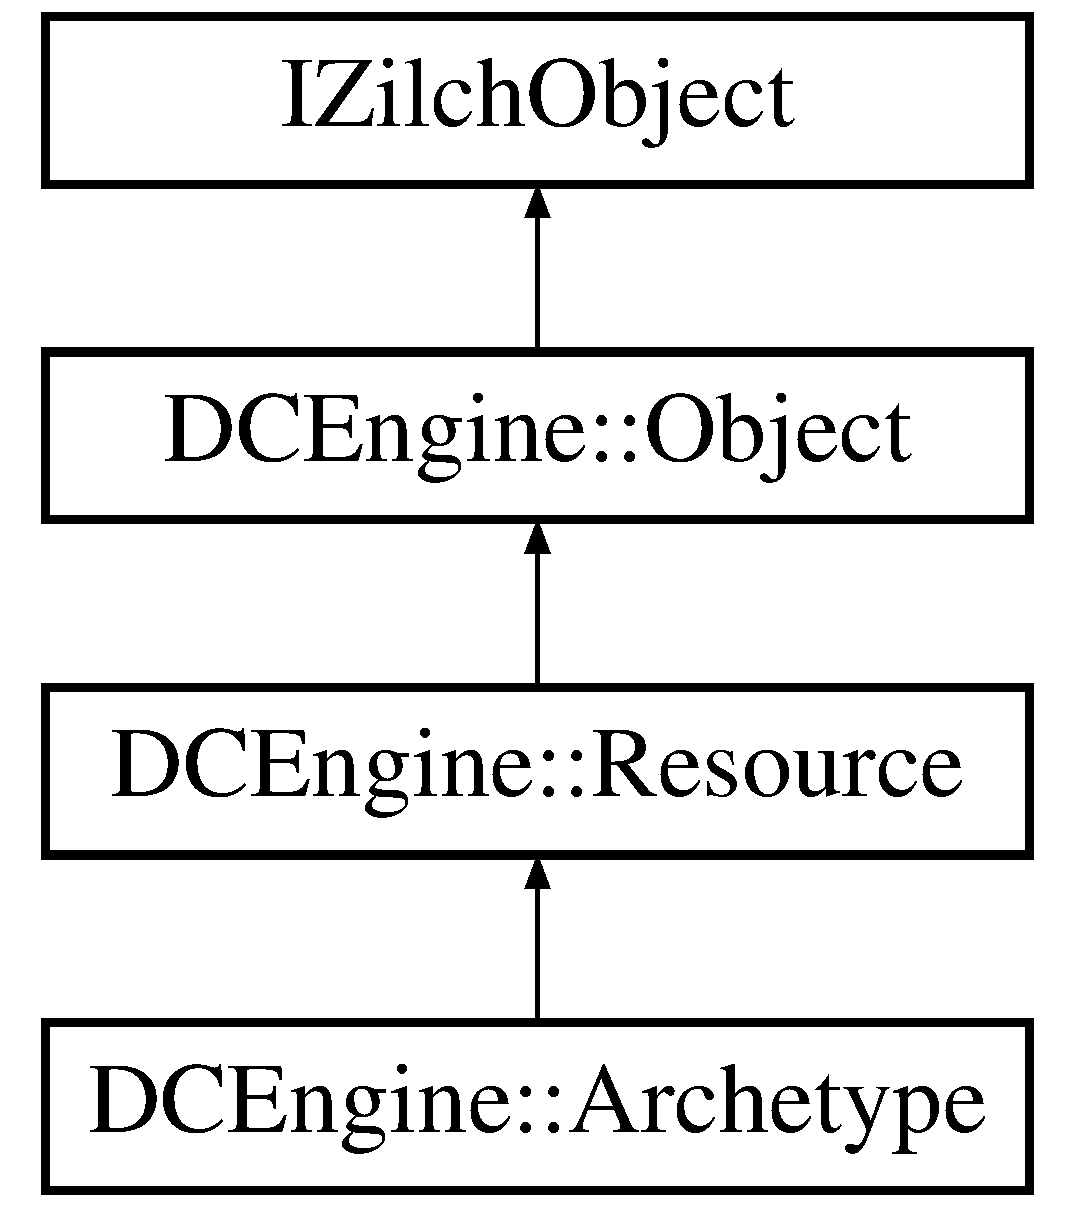
\includegraphics[height=4.000000cm]{classDCEngine_1_1Archetype}
\end{center}
\end{figure}
\subsection*{Public Member Functions}
\begin{DoxyCompactItemize}
\item 
\hyperlink{classDCEngine_1_1Archetype_add655dcfb7a575a8a3b2c05f90cc5608}{Archetype} (std\-::string archetype\-File)
\begin{DoxyCompactList}\small\item\em \hyperlink{classDCEngine_1_1Archetype}{Archetype} constructor. \end{DoxyCompactList}\item 
\hypertarget{classDCEngine_1_1Archetype_a42e05225f820f6ab2c1debaa4083e78d}{{\bfseries Archetype} (std\-::string archetype\-File, std\-::string serialized\-Data)}\label{classDCEngine_1_1Archetype_a42e05225f820f6ab2c1debaa4083e78d}

\item 
\hypertarget{classDCEngine_1_1Archetype_a3fcfb29bcc513063736d04016d249a88}{\hyperlink{classDCEngine_1_1Archetype_a3fcfb29bcc513063736d04016d249a88}{$\sim$\-Archetype} ()}\label{classDCEngine_1_1Archetype_a3fcfb29bcc513063736d04016d249a88}

\begin{DoxyCompactList}\small\item\em \hyperlink{classDCEngine_1_1Archetype}{Archetype} destructor. \end{DoxyCompactList}\item 
\hypertarget{classDCEngine_1_1Archetype_a62445a186a0f9dcf67a446bd7113d082}{void \hyperlink{classDCEngine_1_1Archetype_a62445a186a0f9dcf67a446bd7113d082}{Save} ()}\label{classDCEngine_1_1Archetype_a62445a186a0f9dcf67a446bd7113d082}

\begin{DoxyCompactList}\small\item\em Serializes the data definition of an object from a string back into the source file now that we have modified it. \end{DoxyCompactList}\item 
\hypertarget{classDCEngine_1_1Archetype_ae8d40719f79ca2a5ec7ec40c6a7da65c}{bool \hyperlink{classDCEngine_1_1Archetype_ae8d40719f79ca2a5ec7ec40c6a7da65c}{Load} ()}\label{classDCEngine_1_1Archetype_ae8d40719f79ca2a5ec7ec40c6a7da65c}

\begin{DoxyCompactList}\small\item\em Deserializes the binary cache the serialized data definition of an object into a string that can be parsed by the engine's serializer. \end{DoxyCompactList}\item 
\hypertarget{classDCEngine_1_1Archetype_a57831897d4909bde4a7a1f64abed514c}{const std\-::string \& {\bfseries Get} ()}\label{classDCEngine_1_1Archetype_a57831897d4909bde4a7a1f64abed514c}

\end{DoxyCompactItemize}
\subsection*{Static Public Member Functions}
\begin{DoxyCompactItemize}
\item 
\hypertarget{classDCEngine_1_1Archetype_ab448943ddb438c490910daf8c7335065}{static std\-::string {\bfseries Extension} ()}\label{classDCEngine_1_1Archetype_ab448943ddb438c490910daf8c7335065}

\end{DoxyCompactItemize}
\subsection*{Additional Inherited Members}


\subsection{Constructor \& Destructor Documentation}
\hypertarget{classDCEngine_1_1Archetype_add655dcfb7a575a8a3b2c05f90cc5608}{\index{D\-C\-Engine\-::\-Archetype@{D\-C\-Engine\-::\-Archetype}!Archetype@{Archetype}}
\index{Archetype@{Archetype}!DCEngine::Archetype@{D\-C\-Engine\-::\-Archetype}}
\subsubsection[{Archetype}]{\setlength{\rightskip}{0pt plus 5cm}D\-C\-Engine\-::\-Archetype\-::\-Archetype (
\begin{DoxyParamCaption}
\item[{std\-::string}]{archetype\-File}
\end{DoxyParamCaption}
)}}\label{classDCEngine_1_1Archetype_add655dcfb7a575a8a3b2c05f90cc5608}


\hyperlink{classDCEngine_1_1Archetype}{Archetype} constructor. 


\begin{DoxyParams}{Parameters}
{\em archetype\-File} & \hyperlink{classThe}{The} name of the archetype file. \\
\hline
\end{DoxyParams}


The documentation for this class was generated from the following files\-:\begin{DoxyCompactItemize}
\item 
Core/\-Resources/\hyperlink{Archetype_8h}{Archetype.\-h}\item 
Core/\-Resources/Archetype.\-cpp\end{DoxyCompactItemize}

\hypertarget{structDCEngine_1_1AssetsData}{\section{D\-C\-Engine\-:\-:Assets\-Data Struct Reference}
\label{structDCEngine_1_1AssetsData}\index{D\-C\-Engine\-::\-Assets\-Data@{D\-C\-Engine\-::\-Assets\-Data}}
}
\subsection*{Public Attributes}
\begin{DoxyCompactItemize}
\item 
\hypertarget{structDCEngine_1_1AssetsData_a4081b46a44001df660a05c8c2a629a53}{std\-::string {\bfseries Sprite\-Path}}\label{structDCEngine_1_1AssetsData_a4081b46a44001df660a05c8c2a629a53}

\item 
\hypertarget{structDCEngine_1_1AssetsData_a0324e93c7244faf94a60d74930a73aa6}{std\-::string {\bfseries Sound\-Path}}\label{structDCEngine_1_1AssetsData_a0324e93c7244faf94a60d74930a73aa6}

\item 
\hypertarget{structDCEngine_1_1AssetsData_a864533f5037bd6aba7bddcfd66a94e03}{std\-::string {\bfseries Shader\-Path}}\label{structDCEngine_1_1AssetsData_a864533f5037bd6aba7bddcfd66a94e03}

\item 
\hypertarget{structDCEngine_1_1AssetsData_ae86cec8b75e80abec24246ee595a000d}{std\-::string {\bfseries Font\-Path}}\label{structDCEngine_1_1AssetsData_ae86cec8b75e80abec24246ee595a000d}

\item 
\hypertarget{structDCEngine_1_1AssetsData_ac253a62e53760aa4bb619825b7b8f402}{std\-::string {\bfseries Archetype\-Path}}\label{structDCEngine_1_1AssetsData_ac253a62e53760aa4bb619825b7b8f402}

\item 
\hypertarget{structDCEngine_1_1AssetsData_a357871283992cbbec2d8217f1a5321cb}{std\-::string {\bfseries Level\-Path}}\label{structDCEngine_1_1AssetsData_a357871283992cbbec2d8217f1a5321cb}

\end{DoxyCompactItemize}


The documentation for this struct was generated from the following file\-:\begin{DoxyCompactItemize}
\item 
Core/\-Engine/\hyperlink{Data_8h}{Data.\-h}\end{DoxyCompactItemize}

\hypertarget{classDCEngine_1_1Systems_1_1Audio}{\section{D\-C\-Engine\-:\-:Systems\-:\-:Audio Class Reference}
\label{classDCEngine_1_1Systems_1_1Audio}\index{D\-C\-Engine\-::\-Systems\-::\-Audio@{D\-C\-Engine\-::\-Systems\-::\-Audio}}
}
Inheritance diagram for D\-C\-Engine\-:\-:Systems\-:\-:Audio\-:\begin{figure}[H]
\begin{center}
\leavevmode
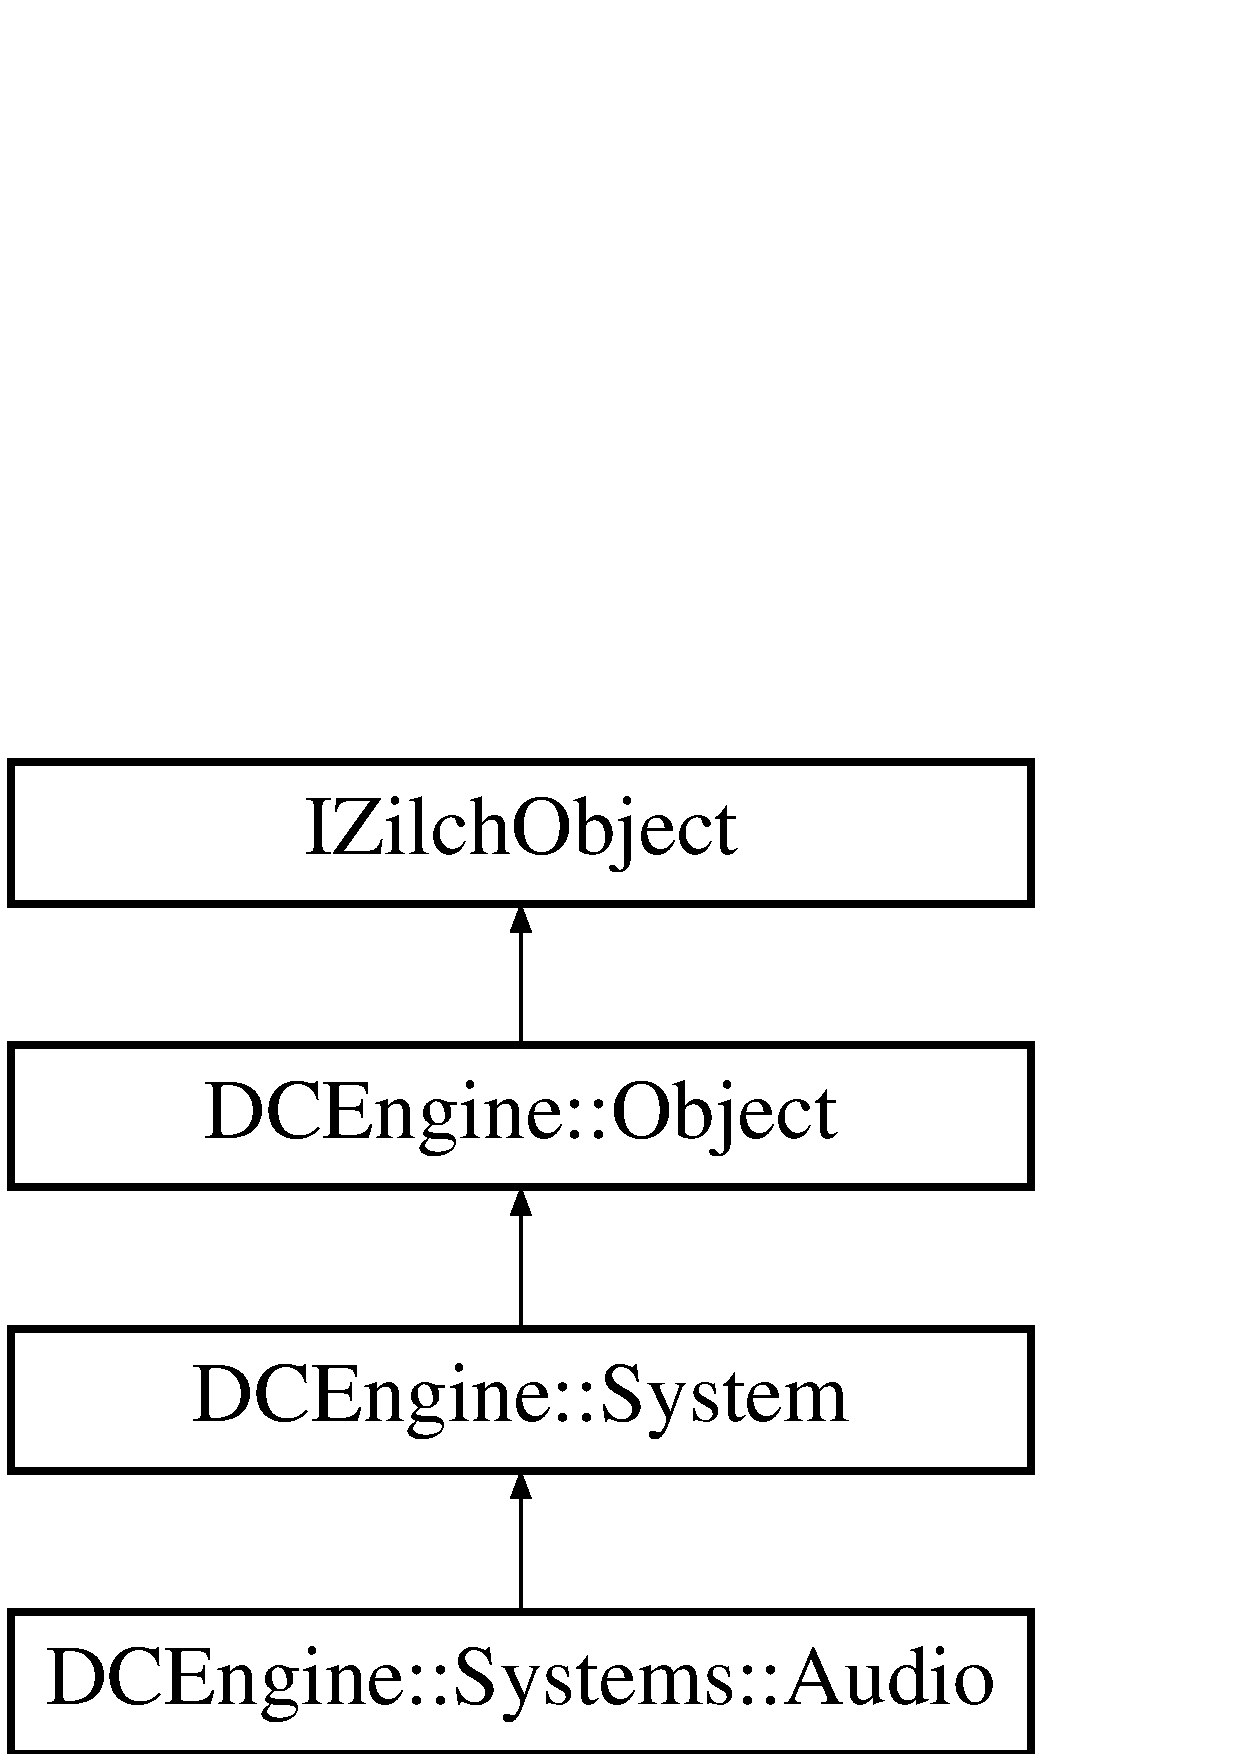
\includegraphics[height=4.000000cm]{classDCEngine_1_1Systems_1_1Audio}
\end{center}
\end{figure}
\subsection*{Public Member Functions}
\begin{DoxyCompactItemize}
\item 
void \hyperlink{classDCEngine_1_1Systems_1_1Audio_a72be5cf056ad0d270796be33a3010fd1}{Add} (std\-::string \&bank\-File, \hyperlink{structDCEngine_1_1Bank_1_1BankData}{Bank\-::\-Bank\-Data} \&data)
\begin{DoxyCompactList}\small\item\em Adds an audio \hyperlink{classDCEngine_1_1Bank}{Bank} to the audio system. \end{DoxyCompactList}\item 
void \hyperlink{classDCEngine_1_1Systems_1_1Audio_a91b9a87f44307937d5f7a597456e1e96}{Create\-Sound} (std\-::string \&sound\-File, \hyperlink{classDCEngine_1_1FMODSoundHandle}{F\-M\-O\-D\-Sound\-Handle} \&sound\-Ptr)
\begin{DoxyCompactList}\small\item\em Registers a Sound\-File to be played through F\-M\-O\-D. \end{DoxyCompactList}\item 
void \hyperlink{classDCEngine_1_1Systems_1_1Audio_a990c57ddc737fd6152bf2f193c41bf46}{Play\-Sound} (std\-::string \&sound\-Cue\-Name)
\begin{DoxyCompactList}\small\item\em Plays a sound cue. \end{DoxyCompactList}\item 
void \hyperlink{classDCEngine_1_1Systems_1_1Audio_a25cef2ad0d520f38089854092caa488e}{Resume\-Sound} (std\-::string \&sound\-Cue\-Name)
\begin{DoxyCompactList}\small\item\em Resumes the playing of a sound. \end{DoxyCompactList}\item 
void \hyperlink{classDCEngine_1_1Systems_1_1Audio_a3cacbad9590e1eb47a8835c342e86742}{Pause\-Sound} (std\-::string \&sound\-Cue\-Name)
\begin{DoxyCompactList}\small\item\em Pauses a sound cue. \end{DoxyCompactList}\item 
void \hyperlink{classDCEngine_1_1Systems_1_1Audio_aaf100dab7a69eb0e1a5068efff6b2774}{Stop\-Sound} (std\-::string \&sound\-Cue\-Name)
\begin{DoxyCompactList}\small\item\em Stops a sound cue. \end{DoxyCompactList}\item 
void \hyperlink{classDCEngine_1_1Systems_1_1Audio_a839f8b25f202211e0828a8bc210d090e}{Register} (\hyperlink{classDCEngine_1_1Components_1_1SoundSpace}{Components\-::\-Sound\-Space} \&sound\-Space)
\begin{DoxyCompactList}\small\item\em Registers a space into the \hyperlink{classDCEngine_1_1Systems_1_1Audio}{Audio} system. \end{DoxyCompactList}\item 
\hypertarget{classDCEngine_1_1Systems_1_1Audio_ac2234c4cff171af0edcb047b6fdf4841}{void \hyperlink{classDCEngine_1_1Systems_1_1Audio_ac2234c4cff171af0edcb047b6fdf4841}{Generate} ()}\label{classDCEngine_1_1Systems_1_1Audio_ac2234c4cff171af0edcb047b6fdf4841}

\begin{DoxyCompactList}\small\item\em Generates audio resources from all currently loaded banks. \end{DoxyCompactList}\end{DoxyCompactItemize}
\subsection*{Friends}
\begin{DoxyCompactItemize}
\item 
\hypertarget{classDCEngine_1_1Systems_1_1Audio_a3e1914489e4bed4f9f23cdeab34a43dc}{class {\bfseries Engine}}\label{classDCEngine_1_1Systems_1_1Audio_a3e1914489e4bed4f9f23cdeab34a43dc}

\item 
\hypertarget{classDCEngine_1_1Systems_1_1Audio_ac6e482d683d1941c834af32656429557}{class {\bfseries Sound\-Space}}\label{classDCEngine_1_1Systems_1_1Audio_ac6e482d683d1941c834af32656429557}

\end{DoxyCompactItemize}
\subsection*{Additional Inherited Members}


\subsection{Member Function Documentation}
\hypertarget{classDCEngine_1_1Systems_1_1Audio_a72be5cf056ad0d270796be33a3010fd1}{\index{D\-C\-Engine\-::\-Systems\-::\-Audio@{D\-C\-Engine\-::\-Systems\-::\-Audio}!Add@{Add}}
\index{Add@{Add}!DCEngine::Systems::Audio@{D\-C\-Engine\-::\-Systems\-::\-Audio}}
\subsubsection[{Add}]{\setlength{\rightskip}{0pt plus 5cm}void D\-C\-Engine\-::\-Systems\-::\-Audio\-::\-Add (
\begin{DoxyParamCaption}
\item[{std\-::string \&}]{bank\-File, }
\item[{{\bf Bank\-::\-Bank\-Data} \&}]{data}
\end{DoxyParamCaption}
)}}\label{classDCEngine_1_1Systems_1_1Audio_a72be5cf056ad0d270796be33a3010fd1}


Adds an audio \hyperlink{classDCEngine_1_1Bank}{Bank} to the audio system. 


\begin{DoxyParams}{Parameters}
{\em bank\-File} & \hyperlink{classThe}{The} name of the bank file. \\
\hline
\end{DoxyParams}
\hypertarget{classDCEngine_1_1Systems_1_1Audio_a91b9a87f44307937d5f7a597456e1e96}{\index{D\-C\-Engine\-::\-Systems\-::\-Audio@{D\-C\-Engine\-::\-Systems\-::\-Audio}!Create\-Sound@{Create\-Sound}}
\index{Create\-Sound@{Create\-Sound}!DCEngine::Systems::Audio@{D\-C\-Engine\-::\-Systems\-::\-Audio}}
\subsubsection[{Create\-Sound}]{\setlength{\rightskip}{0pt plus 5cm}void D\-C\-Engine\-::\-Systems\-::\-Audio\-::\-Create\-Sound (
\begin{DoxyParamCaption}
\item[{std\-::string \&}]{sound\-File, }
\item[{{\bf F\-M\-O\-D\-Sound\-Handle} \&}]{sound\-Ptr}
\end{DoxyParamCaption}
)}}\label{classDCEngine_1_1Systems_1_1Audio_a91b9a87f44307937d5f7a597456e1e96}


Registers a Sound\-File to be played through F\-M\-O\-D. 


\begin{DoxyParams}{Parameters}
{\em sound\-File} & \hyperlink{classThe}{The} name of the sound file. \\
\hline
{\em sound\-Ptr} & A pointer to the F\-M\-O\-D\-Sound pointer. \\
\hline
\end{DoxyParams}
\begin{DoxyRefDesc}{Todo}
\item[\hyperlink{todo__todo000015}{Todo}]Use different functions to create (sound/stream) depending on the file size. \end{DoxyRefDesc}
\hypertarget{classDCEngine_1_1Systems_1_1Audio_a3cacbad9590e1eb47a8835c342e86742}{\index{D\-C\-Engine\-::\-Systems\-::\-Audio@{D\-C\-Engine\-::\-Systems\-::\-Audio}!Pause\-Sound@{Pause\-Sound}}
\index{Pause\-Sound@{Pause\-Sound}!DCEngine::Systems::Audio@{D\-C\-Engine\-::\-Systems\-::\-Audio}}
\subsubsection[{Pause\-Sound}]{\setlength{\rightskip}{0pt plus 5cm}void D\-C\-Engine\-::\-Systems\-::\-Audio\-::\-Pause\-Sound (
\begin{DoxyParamCaption}
\item[{std\-::string \&}]{sound\-Cue\-Name}
\end{DoxyParamCaption}
)}}\label{classDCEngine_1_1Systems_1_1Audio_a3cacbad9590e1eb47a8835c342e86742}


Pauses a sound cue. 


\begin{DoxyParams}{Parameters}
{\em sound\-Cue\-Name} & \hyperlink{classThe}{The} name (string) of the sound in the content system. \\
\hline
\end{DoxyParams}
\hypertarget{classDCEngine_1_1Systems_1_1Audio_a990c57ddc737fd6152bf2f193c41bf46}{\index{D\-C\-Engine\-::\-Systems\-::\-Audio@{D\-C\-Engine\-::\-Systems\-::\-Audio}!Play\-Sound@{Play\-Sound}}
\index{Play\-Sound@{Play\-Sound}!DCEngine::Systems::Audio@{D\-C\-Engine\-::\-Systems\-::\-Audio}}
\subsubsection[{Play\-Sound}]{\setlength{\rightskip}{0pt plus 5cm}void D\-C\-Engine\-::\-Systems\-::\-Audio\-::\-Play\-Sound (
\begin{DoxyParamCaption}
\item[{std\-::string \&}]{sound\-Cue\-Name}
\end{DoxyParamCaption}
)}}\label{classDCEngine_1_1Systems_1_1Audio_a990c57ddc737fd6152bf2f193c41bf46}


Plays a sound cue. 


\begin{DoxyParams}{Parameters}
{\em sound\-Cue\-Name} & \hyperlink{classThe}{The} name (string) of the sound in the content system. \\
\hline
\end{DoxyParams}
\hypertarget{classDCEngine_1_1Systems_1_1Audio_a839f8b25f202211e0828a8bc210d090e}{\index{D\-C\-Engine\-::\-Systems\-::\-Audio@{D\-C\-Engine\-::\-Systems\-::\-Audio}!Register@{Register}}
\index{Register@{Register}!DCEngine::Systems::Audio@{D\-C\-Engine\-::\-Systems\-::\-Audio}}
\subsubsection[{Register}]{\setlength{\rightskip}{0pt plus 5cm}void D\-C\-Engine\-::\-Systems\-::\-Audio\-::\-Register (
\begin{DoxyParamCaption}
\item[{{\bf Components\-::\-Sound\-Space} \&}]{sound\-Space}
\end{DoxyParamCaption}
)}}\label{classDCEngine_1_1Systems_1_1Audio_a839f8b25f202211e0828a8bc210d090e}


Registers a space into the \hyperlink{classDCEngine_1_1Systems_1_1Audio}{Audio} system. 


\begin{DoxyParams}{Parameters}
{\em sound\-Space} & \hyperlink{classThe}{The} 'Sound\-Space' component of the space. \\
\hline
\end{DoxyParams}
\hypertarget{classDCEngine_1_1Systems_1_1Audio_a25cef2ad0d520f38089854092caa488e}{\index{D\-C\-Engine\-::\-Systems\-::\-Audio@{D\-C\-Engine\-::\-Systems\-::\-Audio}!Resume\-Sound@{Resume\-Sound}}
\index{Resume\-Sound@{Resume\-Sound}!DCEngine::Systems::Audio@{D\-C\-Engine\-::\-Systems\-::\-Audio}}
\subsubsection[{Resume\-Sound}]{\setlength{\rightskip}{0pt plus 5cm}void D\-C\-Engine\-::\-Systems\-::\-Audio\-::\-Resume\-Sound (
\begin{DoxyParamCaption}
\item[{std\-::string \&}]{sound\-Cue\-Name}
\end{DoxyParamCaption}
)}}\label{classDCEngine_1_1Systems_1_1Audio_a25cef2ad0d520f38089854092caa488e}


Resumes the playing of a sound. 


\begin{DoxyParams}{Parameters}
{\em sound\-Cue\-Name} & \hyperlink{classThe}{The} name (string) of the sound in the content system. \\
\hline
\end{DoxyParams}
\hypertarget{classDCEngine_1_1Systems_1_1Audio_aaf100dab7a69eb0e1a5068efff6b2774}{\index{D\-C\-Engine\-::\-Systems\-::\-Audio@{D\-C\-Engine\-::\-Systems\-::\-Audio}!Stop\-Sound@{Stop\-Sound}}
\index{Stop\-Sound@{Stop\-Sound}!DCEngine::Systems::Audio@{D\-C\-Engine\-::\-Systems\-::\-Audio}}
\subsubsection[{Stop\-Sound}]{\setlength{\rightskip}{0pt plus 5cm}void D\-C\-Engine\-::\-Systems\-::\-Audio\-::\-Stop\-Sound (
\begin{DoxyParamCaption}
\item[{std\-::string \&}]{sound\-Cue\-Name}
\end{DoxyParamCaption}
)}}\label{classDCEngine_1_1Systems_1_1Audio_aaf100dab7a69eb0e1a5068efff6b2774}


Stops a sound cue. 


\begin{DoxyParams}{Parameters}
{\em sound\-Cue\-Name} & \hyperlink{classThe}{The} name (string) of the sound in the content system. \\
\hline
\end{DoxyParams}


The documentation for this class was generated from the following files\-:\begin{DoxyCompactItemize}
\item 
Core/\-Systems/\-Audio/\hyperlink{Audio_8h}{Audio.\-h}\item 
Core/\-Systems/\-Audio/\hyperlink{Audio_8cpp}{Audio.\-cpp}\end{DoxyCompactItemize}

\hypertarget{classDCEngine_1_1Systems_1_1AudioFMOD}{\section{D\-C\-Engine\-:\-:Systems\-:\-:Audio\-F\-M\-O\-D Class Reference}
\label{classDCEngine_1_1Systems_1_1AudioFMOD}\index{D\-C\-Engine\-::\-Systems\-::\-Audio\-F\-M\-O\-D@{D\-C\-Engine\-::\-Systems\-::\-Audio\-F\-M\-O\-D}}
}
\subsection*{Public Member Functions}
\begin{DoxyCompactItemize}
\item 
\hypertarget{classDCEngine_1_1Systems_1_1AudioFMOD_ab67b73b6e40b905d950877d1488eb818}{\hyperlink{classDCEngine_1_1Systems_1_1AudioFMOD_ab67b73b6e40b905d950877d1488eb818}{$\sim$\-Audio\-F\-M\-O\-D} ()}\label{classDCEngine_1_1Systems_1_1AudioFMOD_ab67b73b6e40b905d950877d1488eb818}

\begin{DoxyCompactList}\small\item\em Destructor for the \hyperlink{classDCEngine_1_1Systems_1_1AudioFMOD}{Audio\-F\-M\-O\-D} class. \end{DoxyCompactList}\item 
bool \hyperlink{classDCEngine_1_1Systems_1_1AudioFMOD_ab5869328256aa9429c8b486a2de9bc5e}{Play\-Sound} (F\-M\-O\-D\-::\-Sound $\ast$sound\-Ptr, F\-M\-O\-D\-::\-Channel $\ast$$\ast$channel, \hyperlink{structDCEngine_1_1Systems_1_1PlaybackSettings}{Playback\-Settings} \&settings)
\begin{DoxyCompactList}\small\item\em Plays a sound through F\-M\-O\-D Low\-Level A\-P\-I. \end{DoxyCompactList}\item 
bool \hyperlink{classDCEngine_1_1Systems_1_1AudioFMOD_a0b753ebc1c4591f15892fdf065f0b2f3}{Play\-Sound} (Event\-Description\-Handle \&event\-Handle, \hyperlink{structDCEngine_1_1Systems_1_1PlaybackSettings}{Playback\-Settings} \&settings)
\begin{DoxyCompactList}\small\item\em Plays a sound through F\-M\-O\-D Studio A\-P\-I. \end{DoxyCompactList}\item 
\hypertarget{classDCEngine_1_1Systems_1_1AudioFMOD_a117772d95e7b83324a03f83e5e4b5b40}{void \hyperlink{classDCEngine_1_1Systems_1_1AudioFMOD_a117772d95e7b83324a03f83e5e4b5b40}{Resume\-Sound} (F\-M\-O\-D\-::\-Channel $\ast$channel)}\label{classDCEngine_1_1Systems_1_1AudioFMOD_a117772d95e7b83324a03f83e5e4b5b40}

\begin{DoxyCompactList}\small\item\em Resumes the playing of a sound through F\-M\-O\-D. \end{DoxyCompactList}\item 
\hypertarget{classDCEngine_1_1Systems_1_1AudioFMOD_af4f086e8b9b8c7c49dc905ca7e292937}{void {\bfseries Resume\-Sound} (Event\-Description\-Handle \&event\-Handle)}\label{classDCEngine_1_1Systems_1_1AudioFMOD_af4f086e8b9b8c7c49dc905ca7e292937}

\item 
\hypertarget{classDCEngine_1_1Systems_1_1AudioFMOD_a01bf69a8da963ba4b622378f81f50858}{void \hyperlink{classDCEngine_1_1Systems_1_1AudioFMOD_a01bf69a8da963ba4b622378f81f50858}{Pause\-Sound} (F\-M\-O\-D\-::\-Channel $\ast$channel)}\label{classDCEngine_1_1Systems_1_1AudioFMOD_a01bf69a8da963ba4b622378f81f50858}

\begin{DoxyCompactList}\small\item\em Stops a sound from playing through F\-M\-O\-D. \end{DoxyCompactList}\item 
\hypertarget{classDCEngine_1_1Systems_1_1AudioFMOD_abd17e801ce9ad5e42478a456387601ba}{void {\bfseries Pause\-Sound} (Event\-Description\-Handle \&event\-Handle)}\label{classDCEngine_1_1Systems_1_1AudioFMOD_abd17e801ce9ad5e42478a456387601ba}

\item 
\hypertarget{classDCEngine_1_1Systems_1_1AudioFMOD_a9d26255a2b865097ca482ee6b5f07756}{void \hyperlink{classDCEngine_1_1Systems_1_1AudioFMOD_a9d26255a2b865097ca482ee6b5f07756}{Stop\-Sound} (F\-M\-O\-D\-::\-Channel $\ast$channel)}\label{classDCEngine_1_1Systems_1_1AudioFMOD_a9d26255a2b865097ca482ee6b5f07756}

\begin{DoxyCompactList}\small\item\em Stops a sound from playing through F\-M\-O\-D Low \hyperlink{classDCEngine_1_1Level}{Level}. \end{DoxyCompactList}\item 
\hypertarget{classDCEngine_1_1Systems_1_1AudioFMOD_a3a35f0d255c26328650b23461bd2981e}{void \hyperlink{classDCEngine_1_1Systems_1_1AudioFMOD_a3a35f0d255c26328650b23461bd2981e}{Stop\-Sound} (Event\-Description\-Handle \&event\-Handle)}\label{classDCEngine_1_1Systems_1_1AudioFMOD_a3a35f0d255c26328650b23461bd2981e}

\begin{DoxyCompactList}\small\item\em Stops a sound from playing through F\-M\-O\-D Studio. \end{DoxyCompactList}\item 
\hypertarget{classDCEngine_1_1Systems_1_1AudioFMOD_ada4aad9a3e46fcfdb442299577d7fd92}{void {\bfseries Stop\-All} ()}\label{classDCEngine_1_1Systems_1_1AudioFMOD_ada4aad9a3e46fcfdb442299577d7fd92}

\item 
\hypertarget{classDCEngine_1_1Systems_1_1AudioFMOD_aafd2f1a9ff50ba390c324ae4eac7bc04}{void {\bfseries Set\-Volume} (F\-M\-O\-D\-::\-Channel $\ast$sound\-Ptr, float volume)}\label{classDCEngine_1_1Systems_1_1AudioFMOD_aafd2f1a9ff50ba390c324ae4eac7bc04}

\item 
\hypertarget{classDCEngine_1_1Systems_1_1AudioFMOD_a166a673b4118f283b09d93006716b226}{void {\bfseries Set\-Volume} (Event\-Description\-Handle \&event\-Handle, float volume)}\label{classDCEngine_1_1Systems_1_1AudioFMOD_a166a673b4118f283b09d93006716b226}

\item 
F\-M\-O\-D\-::\-Studio\-::\-Bank $\ast$ \hyperlink{classDCEngine_1_1Systems_1_1AudioFMOD_a571388ad63c66873859ca886260b3391}{get\-Bank} (std\-::string handle)
\begin{DoxyCompactList}\small\item\em Retrieves a pointer to a given sound bank. \end{DoxyCompactList}\item 
\hypertarget{classDCEngine_1_1Systems_1_1AudioFMOD_a8723ee1355d7015ad233574de0732dd2}{F\-M\-O\-D\-\_\-\-R\-E\-S\-U\-L\-T {\bfseries get\-Bank} (std\-::string path, F\-M\-O\-D\-::\-Studio\-::\-Bank $\ast$$\ast$bank)}\label{classDCEngine_1_1Systems_1_1AudioFMOD_a8723ee1355d7015ad233574de0732dd2}

\item 
F\-M\-O\-D\-::\-Studio\-::\-Bus $\ast$ \hyperlink{classDCEngine_1_1Systems_1_1AudioFMOD_a6a258f8de2af79c25ce96642a03e6851}{get\-Bus} (std\-::string path)
\begin{DoxyCompactList}\small\item\em Retrieves the bus. \end{DoxyCompactList}\item 
\hypertarget{classDCEngine_1_1Systems_1_1AudioFMOD_acbea7bbdf138165c62d1419397f08827}{F\-M\-O\-D\-\_\-\-R\-E\-S\-U\-L\-T {\bfseries get\-Bus} (std\-::string path, F\-M\-O\-D\-::\-Studio\-::\-Bus $\ast$$\ast$bus) const }\label{classDCEngine_1_1Systems_1_1AudioFMOD_acbea7bbdf138165c62d1419397f08827}

\item 
\hypertarget{classDCEngine_1_1Systems_1_1AudioFMOD_a7a944a1adb6fec6891dbc544a565de78}{F\-M\-O\-D\-::\-Studio\-::\-V\-C\-A $\ast$ {\bfseries get\-V\-C\-A} (std\-::string path) const }\label{classDCEngine_1_1Systems_1_1AudioFMOD_a7a944a1adb6fec6891dbc544a565de78}

\item 
\hypertarget{classDCEngine_1_1Systems_1_1AudioFMOD_a68e5d11a5762f20017d45c583f42f9ad}{F\-M\-O\-D\-\_\-\-R\-E\-S\-U\-L\-T {\bfseries get\-V\-C\-A} (std\-::string path, F\-M\-O\-D\-::\-Studio\-::\-V\-C\-A $\ast$$\ast$vca) const }\label{classDCEngine_1_1Systems_1_1AudioFMOD_a68e5d11a5762f20017d45c583f42f9ad}

\item 
\hypertarget{classDCEngine_1_1Systems_1_1AudioFMOD_aa14e87341a443a510872681f9536cf64}{void \hyperlink{classDCEngine_1_1Systems_1_1AudioFMOD_aa14e87341a443a510872681f9536cf64}{Generate\-Resources} ()}\label{classDCEngine_1_1Systems_1_1AudioFMOD_aa14e87341a443a510872681f9536cf64}

\begin{DoxyCompactList}\small\item\em Generates audio resources from all currently loaded banks. \end{DoxyCompactList}\item 
\hypertarget{classDCEngine_1_1Systems_1_1AudioFMOD_a6c00642a03dc8a2733ad6671ff982e92}{void \hyperlink{classDCEngine_1_1Systems_1_1AudioFMOD_a6c00642a03dc8a2733ad6671ff982e92}{Generate\-Sound\-Cues} ()}\label{classDCEngine_1_1Systems_1_1AudioFMOD_a6c00642a03dc8a2733ad6671ff982e92}

\begin{DoxyCompactList}\small\item\em Generates Sound\-Cues from all existing events (Event\-Descriptions). \end{DoxyCompactList}\end{DoxyCompactItemize}
\subsection*{Friends}
\begin{DoxyCompactItemize}
\item 
\hypertarget{classDCEngine_1_1Systems_1_1AudioFMOD_a211f008bd6a46efe478fe81d31e28933}{class {\bfseries Audio}}\label{classDCEngine_1_1Systems_1_1AudioFMOD_a211f008bd6a46efe478fe81d31e28933}

\end{DoxyCompactItemize}


\subsection{Member Function Documentation}
\hypertarget{classDCEngine_1_1Systems_1_1AudioFMOD_a571388ad63c66873859ca886260b3391}{\index{D\-C\-Engine\-::\-Systems\-::\-Audio\-F\-M\-O\-D@{D\-C\-Engine\-::\-Systems\-::\-Audio\-F\-M\-O\-D}!get\-Bank@{get\-Bank}}
\index{get\-Bank@{get\-Bank}!DCEngine::Systems::AudioFMOD@{D\-C\-Engine\-::\-Systems\-::\-Audio\-F\-M\-O\-D}}
\subsubsection[{get\-Bank}]{\setlength{\rightskip}{0pt plus 5cm}F\-M\-O\-D\-::\-Studio\-::\-Bank $\ast$ D\-C\-Engine\-::\-Systems\-::\-Audio\-F\-M\-O\-D\-::get\-Bank (
\begin{DoxyParamCaption}
\item[{std\-::string}]{handle}
\end{DoxyParamCaption}
)}}\label{classDCEngine_1_1Systems_1_1AudioFMOD_a571388ad63c66873859ca886260b3391}


Retrieves a pointer to a given sound bank. 


\begin{DoxyParams}{Parameters}
{\em handle} & \hyperlink{classThe}{The} name of the sound bank. \\
\hline
\end{DoxyParams}
\begin{DoxyReturn}{Returns}
A pointer to the bank. 
\end{DoxyReturn}
\hypertarget{classDCEngine_1_1Systems_1_1AudioFMOD_a6a258f8de2af79c25ce96642a03e6851}{\index{D\-C\-Engine\-::\-Systems\-::\-Audio\-F\-M\-O\-D@{D\-C\-Engine\-::\-Systems\-::\-Audio\-F\-M\-O\-D}!get\-Bus@{get\-Bus}}
\index{get\-Bus@{get\-Bus}!DCEngine::Systems::AudioFMOD@{D\-C\-Engine\-::\-Systems\-::\-Audio\-F\-M\-O\-D}}
\subsubsection[{get\-Bus}]{\setlength{\rightskip}{0pt plus 5cm}F\-M\-O\-D\-::\-Studio\-::\-Bus $\ast$ D\-C\-Engine\-::\-Systems\-::\-Audio\-F\-M\-O\-D\-::get\-Bus (
\begin{DoxyParamCaption}
\item[{std\-::string}]{path}
\end{DoxyParamCaption}
)}}\label{classDCEngine_1_1Systems_1_1AudioFMOD_a6a258f8de2af79c25ce96642a03e6851}


Retrieves the bus. 


\begin{DoxyParams}{Parameters}
{\em path} & \hyperlink{classThe}{The} path to the bus. \\
\hline
\end{DoxyParams}
\begin{DoxyReturn}{Returns}

\end{DoxyReturn}
\hypertarget{classDCEngine_1_1Systems_1_1AudioFMOD_ab5869328256aa9429c8b486a2de9bc5e}{\index{D\-C\-Engine\-::\-Systems\-::\-Audio\-F\-M\-O\-D@{D\-C\-Engine\-::\-Systems\-::\-Audio\-F\-M\-O\-D}!Play\-Sound@{Play\-Sound}}
\index{Play\-Sound@{Play\-Sound}!DCEngine::Systems::AudioFMOD@{D\-C\-Engine\-::\-Systems\-::\-Audio\-F\-M\-O\-D}}
\subsubsection[{Play\-Sound}]{\setlength{\rightskip}{0pt plus 5cm}bool D\-C\-Engine\-::\-Systems\-::\-Audio\-F\-M\-O\-D\-::\-Play\-Sound (
\begin{DoxyParamCaption}
\item[{F\-M\-O\-D\-::\-Sound $\ast$}]{handle, }
\item[{F\-M\-O\-D\-::\-Channel $\ast$$\ast$}]{channel, }
\item[{{\bf Playback\-Settings} \&}]{settings}
\end{DoxyParamCaption}
)}}\label{classDCEngine_1_1Systems_1_1AudioFMOD_ab5869328256aa9429c8b486a2de9bc5e}


Plays a sound through F\-M\-O\-D Low\-Level A\-P\-I. 


\begin{DoxyParams}{Parameters}
{\em sound\-Ptr} & A pointer to the Sound data. \\
\hline
{\em channel} & A pointer to the Channel handle. \\
\hline
{\em loop} & Whether the sound should be played in a loop. \\
\hline
\end{DoxyParams}
\hypertarget{classDCEngine_1_1Systems_1_1AudioFMOD_a0b753ebc1c4591f15892fdf065f0b2f3}{\index{D\-C\-Engine\-::\-Systems\-::\-Audio\-F\-M\-O\-D@{D\-C\-Engine\-::\-Systems\-::\-Audio\-F\-M\-O\-D}!Play\-Sound@{Play\-Sound}}
\index{Play\-Sound@{Play\-Sound}!DCEngine::Systems::AudioFMOD@{D\-C\-Engine\-::\-Systems\-::\-Audio\-F\-M\-O\-D}}
\subsubsection[{Play\-Sound}]{\setlength{\rightskip}{0pt plus 5cm}bool D\-C\-Engine\-::\-Systems\-::\-Audio\-F\-M\-O\-D\-::\-Play\-Sound (
\begin{DoxyParamCaption}
\item[{Event\-Description\-Handle \&}]{event\-Name, }
\item[{{\bf Playback\-Settings} \&}]{settings}
\end{DoxyParamCaption}
)}}\label{classDCEngine_1_1Systems_1_1AudioFMOD_a0b753ebc1c4591f15892fdf065f0b2f3}


Plays a sound through F\-M\-O\-D Studio A\-P\-I. 


\begin{DoxyParams}{Parameters}
{\em event\-Description} & \hyperlink{classThe}{The} event which to play. \\
\hline
\end{DoxyParams}


The documentation for this class was generated from the following files\-:\begin{DoxyCompactItemize}
\item 
Core/\-Systems/\-Audio/\hyperlink{AudioFMOD_8h}{Audio\-F\-M\-O\-D.\-h}\item 
Core/\-Systems/\-Audio/\hyperlink{AudioFMOD_8cpp}{Audio\-F\-M\-O\-D.\-cpp}\item 
Core/\-Systems/\-Audio/\hyperlink{AudioFMOD__Add_8cpp}{Audio\-F\-M\-O\-D\-\_\-\-Add.\-cpp}\item 
Core/\-Systems/\-Audio/\hyperlink{AudioFMOD__Get_8cpp}{Audio\-F\-M\-O\-D\-\_\-\-Get.\-cpp}\item 
Core/\-Systems/\-Audio/\hyperlink{AudioFMOD__Playback_8cpp}{Audio\-F\-M\-O\-D\-\_\-\-Playback.\-cpp}\end{DoxyCompactItemize}

\hypertarget{structDCEngine_1_1Systems_1_1AudioFMODSettings}{\section{D\-C\-Engine\-:\-:Systems\-:\-:Audio\-F\-M\-O\-D\-Settings Struct Reference}
\label{structDCEngine_1_1Systems_1_1AudioFMODSettings}\index{D\-C\-Engine\-::\-Systems\-::\-Audio\-F\-M\-O\-D\-Settings@{D\-C\-Engine\-::\-Systems\-::\-Audio\-F\-M\-O\-D\-Settings}}
}
\subsection*{Public Attributes}
\begin{DoxyCompactItemize}
\item 
\hypertarget{structDCEngine_1_1Systems_1_1AudioFMODSettings_a706bdcbdc7c9436aa7091c15e456942a}{unsigned {\bfseries Max\-Channels}}\label{structDCEngine_1_1Systems_1_1AudioFMODSettings_a706bdcbdc7c9436aa7091c15e456942a}

\item 
\hypertarget{structDCEngine_1_1Systems_1_1AudioFMODSettings_a80409fe23dce4333c7335028a20b1995}{unsigned {\bfseries Volume}}\label{structDCEngine_1_1Systems_1_1AudioFMODSettings_a80409fe23dce4333c7335028a20b1995}

\item 
\hypertarget{structDCEngine_1_1Systems_1_1AudioFMODSettings_a886a91dd7b3f79c48f95e54f2c2a456f}{unsigned {\bfseries Pitch}}\label{structDCEngine_1_1Systems_1_1AudioFMODSettings_a886a91dd7b3f79c48f95e54f2c2a456f}

\item 
\hypertarget{structDCEngine_1_1Systems_1_1AudioFMODSettings_a39e6622a3514d031679b7a52b3f889de}{bool {\bfseries Paused}}\label{structDCEngine_1_1Systems_1_1AudioFMODSettings_a39e6622a3514d031679b7a52b3f889de}

\item 
\hypertarget{structDCEngine_1_1Systems_1_1AudioFMODSettings_ace7ae1e8ed099c55d78876f5dd9a146a}{float {\bfseries Level}}\label{structDCEngine_1_1Systems_1_1AudioFMODSettings_ace7ae1e8ed099c55d78876f5dd9a146a}

\item 
\hypertarget{structDCEngine_1_1Systems_1_1AudioFMODSettings_af9be4d854e50e532bc8b236ad7d47dff}{bool {\bfseries Muted}}\label{structDCEngine_1_1Systems_1_1AudioFMODSettings_af9be4d854e50e532bc8b236ad7d47dff}

\end{DoxyCompactItemize}


The documentation for this struct was generated from the following file\-:\begin{DoxyCompactItemize}
\item 
Core/\-Systems/\-Audio/\hyperlink{AudioFMOD__Utilities_8h}{Audio\-F\-M\-O\-D\-\_\-\-Utilities.\-h}\end{DoxyCompactItemize}

\hypertarget{classDCEngine_1_1Components_1_1BallController}{\section{D\-C\-Engine\-:\-:Components\-:\-:Ball\-Controller Class Reference}
\label{classDCEngine_1_1Components_1_1BallController}\index{D\-C\-Engine\-::\-Components\-::\-Ball\-Controller@{D\-C\-Engine\-::\-Components\-::\-Ball\-Controller}}
}
Inheritance diagram for D\-C\-Engine\-:\-:Components\-:\-:Ball\-Controller\-:\begin{figure}[H]
\begin{center}
\leavevmode
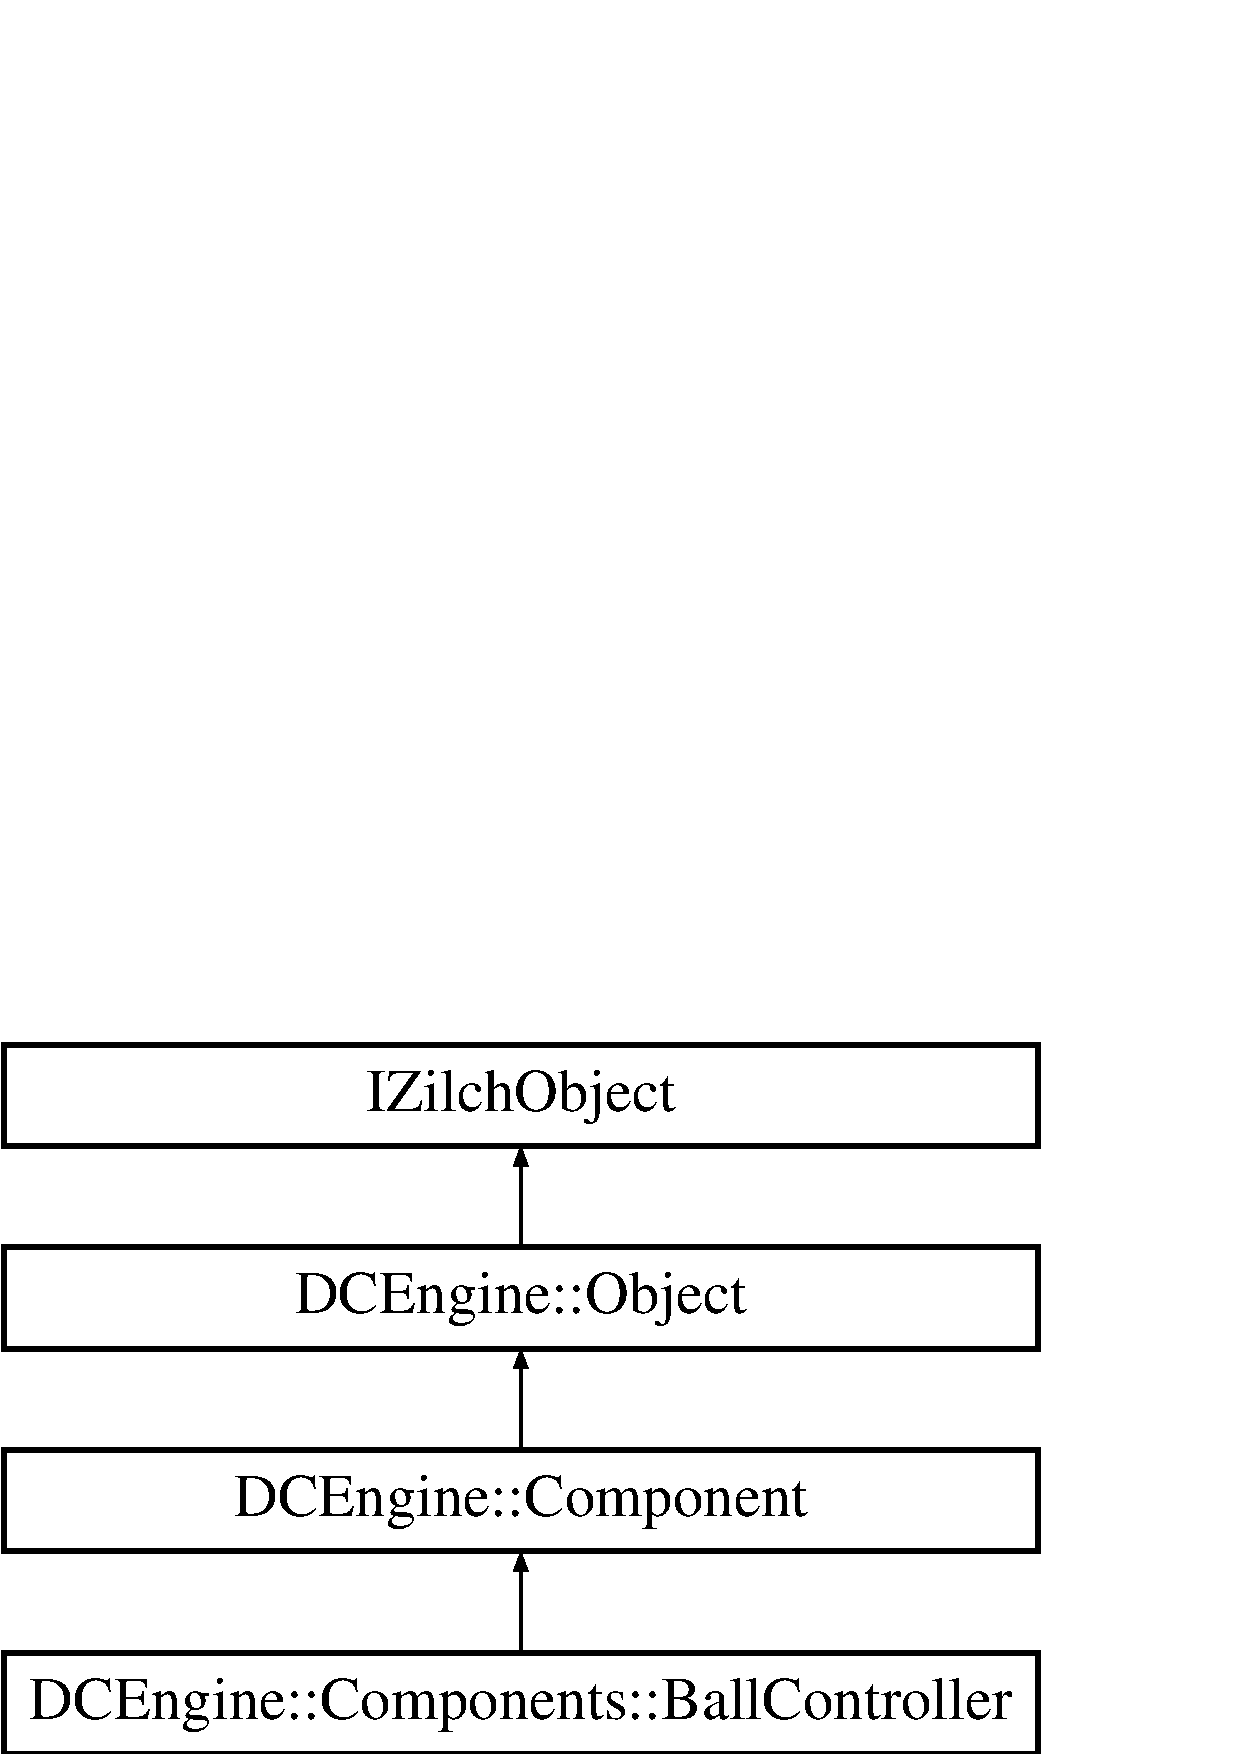
\includegraphics[height=4.000000cm]{classDCEngine_1_1Components_1_1BallController}
\end{center}
\end{figure}
\subsection*{Public Member Functions}
\begin{DoxyCompactItemize}
\item 
\hypertarget{classDCEngine_1_1Components_1_1BallController_a64dc96f10b908e0f0a8e7ba913570311}{{\bfseries D\-C\-E\-\_\-\-D\-E\-F\-I\-N\-E\-\_\-\-P\-R\-O\-P\-E\-R\-T\-Y} (String, Player\-Name)}\label{classDCEngine_1_1Components_1_1BallController_a64dc96f10b908e0f0a8e7ba913570311}

\item 
\hypertarget{classDCEngine_1_1Components_1_1BallController_a7ef101c85388d061ae7091f331483690}{{\bfseries D\-C\-E\-\_\-\-D\-E\-F\-I\-N\-E\-\_\-\-P\-R\-O\-P\-E\-R\-T\-Y} (Real, Move\-Speed)}\label{classDCEngine_1_1Components_1_1BallController_a7ef101c85388d061ae7091f331483690}

\item 
\hypertarget{classDCEngine_1_1Components_1_1BallController_a4b334d4d664a7afc7e5e12737f9e3c8a}{{\bfseries D\-C\-E\-\_\-\-D\-E\-F\-I\-N\-E\-\_\-\-P\-R\-O\-P\-E\-R\-T\-Y} (Real, Rot\-Speed)}\label{classDCEngine_1_1Components_1_1BallController_a4b334d4d664a7afc7e5e12737f9e3c8a}

\item 
\hypertarget{classDCEngine_1_1Components_1_1BallController_ad0316466b881fb715f6a2ef3f1a18f78}{{\bfseries D\-C\-E\-\_\-\-D\-E\-F\-I\-N\-E\-\_\-\-P\-R\-O\-P\-E\-R\-T\-Y} (Real, Current\-Charge)}\label{classDCEngine_1_1Components_1_1BallController_ad0316466b881fb715f6a2ef3f1a18f78}

\item 
\hypertarget{classDCEngine_1_1Components_1_1BallController_aad3e2d5000447311a1783bc5ecd4256b}{{\bfseries D\-C\-E\-\_\-\-D\-E\-F\-I\-N\-E\-\_\-\-P\-R\-O\-P\-E\-R\-T\-Y} (Real, Max\-Charge)}\label{classDCEngine_1_1Components_1_1BallController_aad3e2d5000447311a1783bc5ecd4256b}

\item 
\hypertarget{classDCEngine_1_1Components_1_1BallController_a724bde15800b948594eaf31cdb9129c9}{{\bfseries D\-C\-E\-\_\-\-D\-E\-F\-I\-N\-E\-\_\-\-P\-R\-O\-P\-E\-R\-T\-Y} (Real, Min\-Charge)}\label{classDCEngine_1_1Components_1_1BallController_a724bde15800b948594eaf31cdb9129c9}

\item 
\hypertarget{classDCEngine_1_1Components_1_1BallController_a0fed2dbf7f3bbe8296db7d17cdf709a5}{{\bfseries D\-C\-E\-\_\-\-D\-E\-F\-I\-N\-E\-\_\-\-P\-R\-O\-P\-E\-R\-T\-Y} (Vec4, Frozen\-Color)}\label{classDCEngine_1_1Components_1_1BallController_a0fed2dbf7f3bbe8296db7d17cdf709a5}

\item 
\hypertarget{classDCEngine_1_1Components_1_1BallController_a73a5eab7acf22b56c71c3a402c5b5116}{{\bfseries D\-C\-E\-\_\-\-D\-E\-F\-I\-N\-E\-\_\-\-P\-R\-O\-P\-E\-R\-T\-Y} (Vec4, Normal\-Color)}\label{classDCEngine_1_1Components_1_1BallController_a73a5eab7acf22b56c71c3a402c5b5116}

\item 
\hypertarget{classDCEngine_1_1Components_1_1BallController_a4d8874dd2d2a042a4b9f87fdeb743422}{{\bfseries D\-C\-E\-\_\-\-D\-E\-F\-I\-N\-E\-\_\-\-P\-R\-O\-P\-E\-R\-T\-Y} (Vec4, Charged\-Color)}\label{classDCEngine_1_1Components_1_1BallController_a4d8874dd2d2a042a4b9f87fdeb743422}

\item 
\hypertarget{classDCEngine_1_1Components_1_1BallController_a3df54004e15b20f6be79d903532b86bc}{{\bfseries D\-C\-E\-\_\-\-D\-E\-F\-I\-N\-E\-\_\-\-P\-R\-O\-P\-E\-R\-T\-Y} (Boolean, Freeze\-Enabled)}\label{classDCEngine_1_1Components_1_1BallController_a3df54004e15b20f6be79d903532b86bc}

\item 
\hypertarget{classDCEngine_1_1Components_1_1BallController_aa0047b5655e2296bfd9fa30c1e6f36be}{{\bfseries D\-C\-E\-\_\-\-D\-E\-F\-I\-N\-E\-\_\-\-P\-R\-O\-P\-E\-R\-T\-Y} (Boolean, Charging)}\label{classDCEngine_1_1Components_1_1BallController_aa0047b5655e2296bfd9fa30c1e6f36be}

\item 
\hypertarget{classDCEngine_1_1Components_1_1BallController_ad364dd12b757949c220340c7b877f578}{{\bfseries Ball\-Controller} (\hyperlink{classDCEngine_1_1Entity}{Entity} \&owner)}\label{classDCEngine_1_1Components_1_1BallController_ad364dd12b757949c220340c7b877f578}

\item 
\hypertarget{classDCEngine_1_1Components_1_1BallController_a5ebbf5fec14ce06d199fb35e99a714cb}{void {\bfseries Initialize} ()}\label{classDCEngine_1_1Components_1_1BallController_a5ebbf5fec14ce06d199fb35e99a714cb}

\item 
\hypertarget{classDCEngine_1_1Components_1_1BallController_a95992572a0263f93aa74ef019085df7b}{virtual void {\bfseries Serialize} (Json\-::\-Value \&root)}\label{classDCEngine_1_1Components_1_1BallController_a95992572a0263f93aa74ef019085df7b}

\item 
\hypertarget{classDCEngine_1_1Components_1_1BallController_a409da8e1de1833b022cda4506bd59194}{virtual void {\bfseries Deserialize} (Json\-::\-Value \&root)}\label{classDCEngine_1_1Components_1_1BallController_a409da8e1de1833b022cda4506bd59194}

\item 
\hypertarget{classDCEngine_1_1Components_1_1BallController_a89e7742a6c3ae6ad9ac6f8458b049f69}{void {\bfseries On\-Mouse\-Down\-Event} (\hyperlink{classDCEngine_1_1Events_1_1MouseDown}{Events\-::\-Mouse\-Down} $\ast$event)}\label{classDCEngine_1_1Components_1_1BallController_a89e7742a6c3ae6ad9ac6f8458b049f69}

\item 
\hypertarget{classDCEngine_1_1Components_1_1BallController_a84f53a65965c025e733a2c3f0a5b1446}{void {\bfseries On\-Mouse\-Up\-Event} (\hyperlink{classDCEngine_1_1Events_1_1MouseUp}{Events\-::\-Mouse\-Up} $\ast$event)}\label{classDCEngine_1_1Components_1_1BallController_a84f53a65965c025e733a2c3f0a5b1446}

\item 
\hypertarget{classDCEngine_1_1Components_1_1BallController_ab61330767f04f4c6b55ce21578025226}{void {\bfseries On\-Collision\-Started\-Event} (\hyperlink{classDCEngine_1_1Events_1_1CollisionStarted}{Events\-::\-Collision\-Started} $\ast$event)}\label{classDCEngine_1_1Components_1_1BallController_ab61330767f04f4c6b55ce21578025226}

\item 
\hypertarget{classDCEngine_1_1Components_1_1BallController_afed2cde053e29c4beb7c800812e42f18}{void {\bfseries On\-Collision\-Ended\-Event} (\hyperlink{classDCEngine_1_1Events_1_1CollisionEnded}{Events\-::\-Collision\-Ended} $\ast$event)}\label{classDCEngine_1_1Components_1_1BallController_afed2cde053e29c4beb7c800812e42f18}

\item 
\hypertarget{classDCEngine_1_1Components_1_1BallController_a53e079f6c64d38f9821b34a94dc13462}{void {\bfseries Ball\-Controller\-::\-On\-Logic\-Update\-Event} (\hyperlink{classDCEngine_1_1Events_1_1LogicUpdate}{Events\-::\-Logic\-Update} $\ast$event)}\label{classDCEngine_1_1Components_1_1BallController_a53e079f6c64d38f9821b34a94dc13462}

\item 
\hypertarget{classDCEngine_1_1Components_1_1BallController_a721910d51ebbfc9db357a63fdee9c9d0}{void {\bfseries Change\-Color} ()}\label{classDCEngine_1_1Components_1_1BallController_a721910d51ebbfc9db357a63fdee9c9d0}

\item 
\hypertarget{classDCEngine_1_1Components_1_1BallController_a1ef1efab56ebee8576be62ec44abc387}{{\bfseries Zilch\-Declare\-Derived\-Type} (\hyperlink{classDCEngine_1_1Components_1_1BallController}{Ball\-Controller}, \hyperlink{classDCEngine_1_1Component}{Component})}\label{classDCEngine_1_1Components_1_1BallController_a1ef1efab56ebee8576be62ec44abc387}

\end{DoxyCompactItemize}
\subsection*{Public Attributes}
\begin{DoxyCompactItemize}
\item 
\hypertarget{classDCEngine_1_1Components_1_1BallController_a696af17372a72b15f1fa26b129f16883}{bool {\bfseries Translation} = true}\label{classDCEngine_1_1Components_1_1BallController_a696af17372a72b15f1fa26b129f16883}

\item 
\hypertarget{classDCEngine_1_1Components_1_1BallController_adb1bf393d426d986abbda1631ad60e9f}{bool {\bfseries Frozen} = false}\label{classDCEngine_1_1Components_1_1BallController_adb1bf393d426d986abbda1631ad60e9f}

\item 
\hypertarget{classDCEngine_1_1Components_1_1BallController_a65c546f9f04910ff579bc017cb161cd1}{bool {\bfseries Locked} = false}\label{classDCEngine_1_1Components_1_1BallController_a65c546f9f04910ff579bc017cb161cd1}

\item 
\hypertarget{classDCEngine_1_1Components_1_1BallController_a98b551a71bccff201115dd38225916a6}{Boolean {\bfseries Powering} = false}\label{classDCEngine_1_1Components_1_1BallController_a98b551a71bccff201115dd38225916a6}

\item 
\hypertarget{classDCEngine_1_1Components_1_1BallController_ad24cde2fb8ccb87230a925b15cf0f8ee}{bool {\bfseries Currently\-Fired} = false}\label{classDCEngine_1_1Components_1_1BallController_ad24cde2fb8ccb87230a925b15cf0f8ee}

\item 
\hypertarget{classDCEngine_1_1Components_1_1BallController_a0c0f2d4c260e4ed2fe13c46581d55b57}{Real {\bfseries Move\-Speed} = 0.\-75}\label{classDCEngine_1_1Components_1_1BallController_a0c0f2d4c260e4ed2fe13c46581d55b57}

\item 
\hypertarget{classDCEngine_1_1Components_1_1BallController_a7e27311d1be2db845f9c1f225c2619eb}{Control\-Scheme {\bfseries Control\-Scheme} = Control\-Scheme\-::\-John}\label{classDCEngine_1_1Components_1_1BallController_a7e27311d1be2db845f9c1f225c2619eb}

\item 
\hypertarget{classDCEngine_1_1Components_1_1BallController_a320a0d87553ffe869863de6e77d55bdf}{Real {\bfseries Rot\-Speed} = 15}\label{classDCEngine_1_1Components_1_1BallController_a320a0d87553ffe869863de6e77d55bdf}

\item 
\hypertarget{classDCEngine_1_1Components_1_1BallController_ae217186247941f27661cdaf8984d58e7}{\hyperlink{classDCEngine_1_1Components_1_1Transform}{Transform} $\ast$ {\bfseries Transform\-Ref}}\label{classDCEngine_1_1Components_1_1BallController_ae217186247941f27661cdaf8984d58e7}

\item 
\hypertarget{classDCEngine_1_1Components_1_1BallController_aaeea1b609bf39fe0e02dcaebf845af8f}{\hyperlink{classDCEngine_1_1Components_1_1RigidBody}{Rigid\-Body} $\ast$ {\bfseries Rigid\-Body\-Ref}}\label{classDCEngine_1_1Components_1_1BallController_aaeea1b609bf39fe0e02dcaebf845af8f}

\item 
\hypertarget{classDCEngine_1_1Components_1_1BallController_a3f499b9babc22e72442d93c6f6038816}{\hyperlink{classDCEngine_1_1Components_1_1Sprite}{Sprite} $\ast$ {\bfseries Sprite\-Ref}}\label{classDCEngine_1_1Components_1_1BallController_a3f499b9babc22e72442d93c6f6038816}

\item 
\hypertarget{classDCEngine_1_1Components_1_1BallController_a8ad3e9a9251e51cda9ffd9e174bcaec6}{Real {\bfseries Current\-Charge} = 0}\label{classDCEngine_1_1Components_1_1BallController_a8ad3e9a9251e51cda9ffd9e174bcaec6}

\item 
\hypertarget{classDCEngine_1_1Components_1_1BallController_a4204fb1a23e1e4c3174531b4cdb4f88d}{Real {\bfseries Max\-Charge} = 2}\label{classDCEngine_1_1Components_1_1BallController_a4204fb1a23e1e4c3174531b4cdb4f88d}

\item 
\hypertarget{classDCEngine_1_1Components_1_1BallController_a6c2d6293d1f34002aaa58b18cab5228b}{Real {\bfseries Min\-Charge} = 0.\-5f}\label{classDCEngine_1_1Components_1_1BallController_a6c2d6293d1f34002aaa58b18cab5228b}

\item 
\hypertarget{classDCEngine_1_1Components_1_1BallController_accb4e15e4833574db3e528e1807b1fac}{Real {\bfseries Charge\-Factor} = 30 $\ast$ 1000}\label{classDCEngine_1_1Components_1_1BallController_accb4e15e4833574db3e528e1807b1fac}

\item 
\hypertarget{classDCEngine_1_1Components_1_1BallController_a81a6e45cd0370b4978193200bc44f1ef}{Real {\bfseries Restitution} = 0.\-7}\label{classDCEngine_1_1Components_1_1BallController_a81a6e45cd0370b4978193200bc44f1ef}

\item 
\hypertarget{classDCEngine_1_1Components_1_1BallController_a972149fbf3ebf461dbd46aeda19e18a9}{Real {\bfseries Friction} = 0.\-1}\label{classDCEngine_1_1Components_1_1BallController_a972149fbf3ebf461dbd46aeda19e18a9}

\item 
\hypertarget{classDCEngine_1_1Components_1_1BallController_a6aecf1b2211547e40959e48780a2cf7d}{Real {\bfseries Attract\-Power} = 400.\-0f}\label{classDCEngine_1_1Components_1_1BallController_a6aecf1b2211547e40959e48780a2cf7d}

\item 
\hypertarget{classDCEngine_1_1Components_1_1BallController_a26f5b703eb89aedfc975f197e159e929}{Real {\bfseries Attract\-Y\-Boost} = 3}\label{classDCEngine_1_1Components_1_1BallController_a26f5b703eb89aedfc975f197e159e929}

\item 
\hypertarget{classDCEngine_1_1Components_1_1BallController_a505bd371f2653ad0e7865ad6fa35ed2c}{Boolean {\bfseries Charging} = false}\label{classDCEngine_1_1Components_1_1BallController_a505bd371f2653ad0e7865ad6fa35ed2c}

\item 
\hypertarget{classDCEngine_1_1Components_1_1BallController_a600b1a5e5bf832965fa8945b37a69669}{Boolean {\bfseries Freeze\-Enabled} = true}\label{classDCEngine_1_1Components_1_1BallController_a600b1a5e5bf832965fa8945b37a69669}

\item 
\hypertarget{classDCEngine_1_1Components_1_1BallController_a20e8a00b60f3c0cfa97e2a1a8a9ce31c}{Vec4 {\bfseries Frozen\-Color} = Vec4(1, 0, 1, 1)}\label{classDCEngine_1_1Components_1_1BallController_a20e8a00b60f3c0cfa97e2a1a8a9ce31c}

\item 
\hypertarget{classDCEngine_1_1Components_1_1BallController_a3565602b9e16234b097206729f6b1056}{Vec4 {\bfseries Normal\-Color} = Vec4(0.\-0f, 0.\-7f, 0.\-3f, 1.\-0f)}\label{classDCEngine_1_1Components_1_1BallController_a3565602b9e16234b097206729f6b1056}

\item 
\hypertarget{classDCEngine_1_1Components_1_1BallController_a08b1ebd1b20eb53ad49c599abe5d39f1}{Vec4 {\bfseries Charged\-Color} = Vec4(0.\-0f, 0.\-7f, 1.\-0f, 1.\-0f)}\label{classDCEngine_1_1Components_1_1BallController_a08b1ebd1b20eb53ad49c599abe5d39f1}

\item 
\hypertarget{classDCEngine_1_1Components_1_1BallController_a662d826cd1dfa11d2a0dd572f916c33a}{\hyperlink{classDCEngine_1_1GameObject}{Game\-Object} $\ast$ {\bfseries Player\-Ref}}\label{classDCEngine_1_1Components_1_1BallController_a662d826cd1dfa11d2a0dd572f916c33a}

\item 
\hypertarget{classDCEngine_1_1Components_1_1BallController_a417851071955e3084b1cfe9af73f25b7}{String {\bfseries Player\-Name} = \char`\"{}Player\char`\"{}}\label{classDCEngine_1_1Components_1_1BallController_a417851071955e3084b1cfe9af73f25b7}

\end{DoxyCompactItemize}
\subsection*{Additional Inherited Members}


The documentation for this class was generated from the following files\-:\begin{DoxyCompactItemize}
\item 
Projects/\-Rebound/\-Components/\hyperlink{BallController_8h}{Ball\-Controller.\-h}\item 
Projects/\-Rebound/\-Components/\hyperlink{BallController_8cpp}{Ball\-Controller.\-cpp}\end{DoxyCompactItemize}

\hypertarget{classDCEngine_1_1Bank}{\section{D\-C\-Engine\-:\-:Bank Class Reference}
\label{classDCEngine_1_1Bank}\index{D\-C\-Engine\-::\-Bank@{D\-C\-Engine\-::\-Bank}}
}
Inheritance diagram for D\-C\-Engine\-:\-:Bank\-:\begin{figure}[H]
\begin{center}
\leavevmode
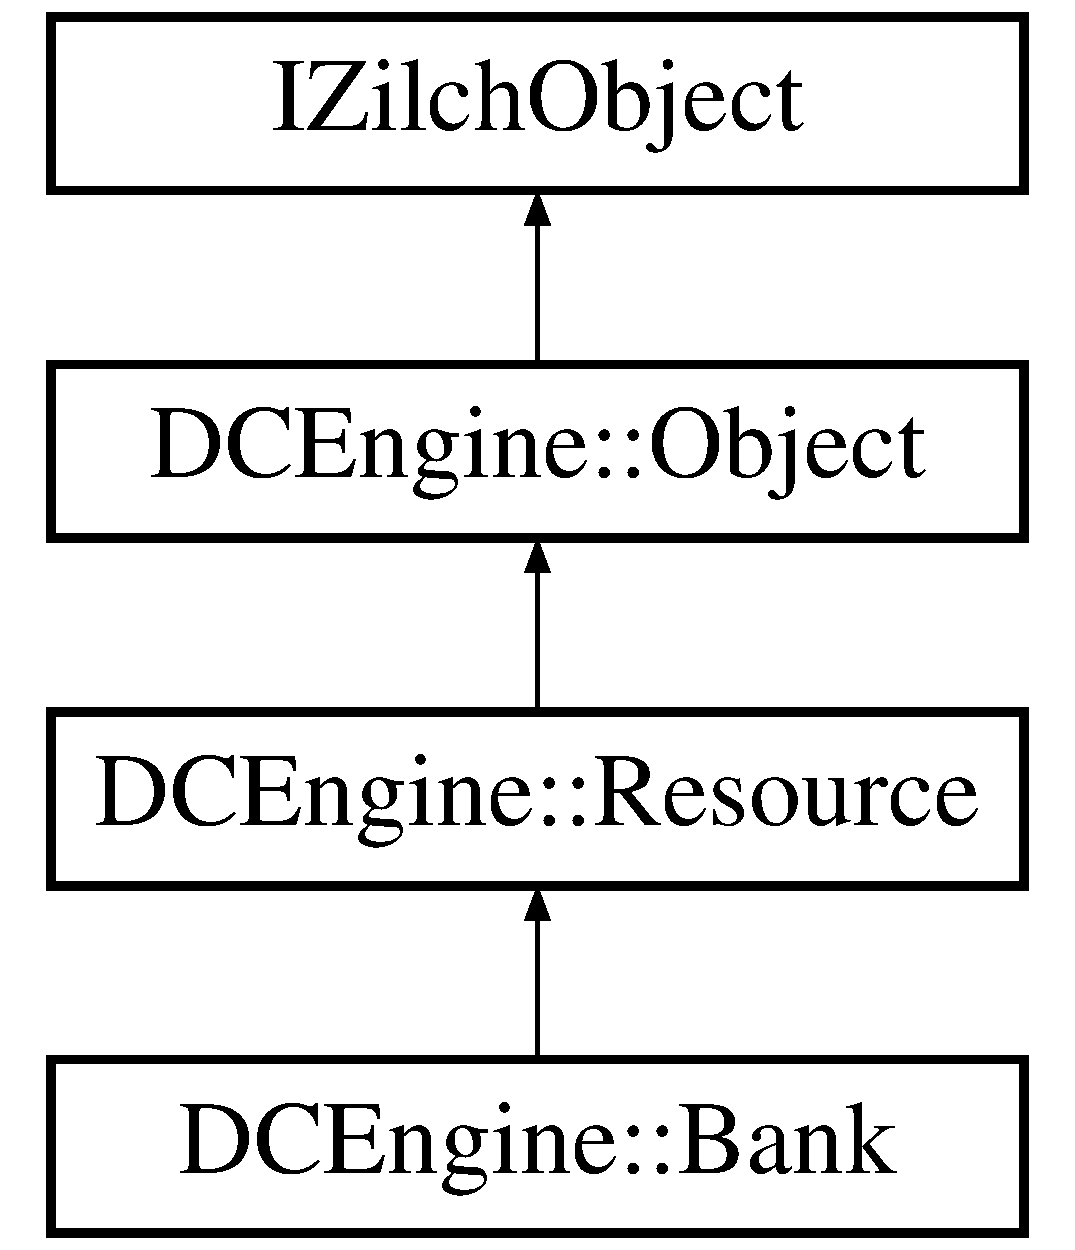
\includegraphics[height=4.000000cm]{classDCEngine_1_1Bank}
\end{center}
\end{figure}
\subsection*{Classes}
\begin{DoxyCompactItemize}
\item 
struct \hyperlink{structDCEngine_1_1Bank_1_1BankData}{Bank\-Data}
\end{DoxyCompactItemize}
\subsection*{Public Member Functions}
\begin{DoxyCompactItemize}
\item 
\hypertarget{classDCEngine_1_1Bank_afd76b244ded7d26fe0d197536d9193bb}{{\bfseries D\-C\-E\-\_\-\-D\-E\-F\-I\-N\-E\-\_\-\-P\-R\-O\-P\-E\-R\-T\-Y} (std\-::string, Asset\-Path)}\label{classDCEngine_1_1Bank_afd76b244ded7d26fe0d197536d9193bb}

\item 
\hypertarget{classDCEngine_1_1Bank_a0fd92945984cae8248c2fa85106fcf15}{void \hyperlink{classDCEngine_1_1Bank_a0fd92945984cae8248c2fa85106fcf15}{Generate} ()}\label{classDCEngine_1_1Bank_a0fd92945984cae8248c2fa85106fcf15}

\begin{DoxyCompactList}\small\item\em Generates a list of Sound\-Cues for every \hyperlink{classDCEngine_1_1Event}{Event} in the bank. \end{DoxyCompactList}\item 
\hypertarget{classDCEngine_1_1Bank_aaf783acc5b1ef653f29e54ec52bd3610}{{\bfseries Zilch\-Declare\-Derived\-Type} (\hyperlink{classDCEngine_1_1Bank}{Bank}, \hyperlink{classDCEngine_1_1Resource}{Resource})}\label{classDCEngine_1_1Bank_aaf783acc5b1ef653f29e54ec52bd3610}

\item 
\hypertarget{classDCEngine_1_1Bank_ae83da3f3d70606509782927cf08e227b}{\hyperlink{classDCEngine_1_1Bank_ae83da3f3d70606509782927cf08e227b}{Bank} (std\-::string name)}\label{classDCEngine_1_1Bank_ae83da3f3d70606509782927cf08e227b}

\begin{DoxyCompactList}\small\item\em \hyperlink{classDCEngine_1_1CollisionGroup}{Collision\-Group} constructor. \end{DoxyCompactList}\end{DoxyCompactItemize}
\subsection*{Static Public Member Functions}
\begin{DoxyCompactItemize}
\item 
\hypertarget{classDCEngine_1_1Bank_af4b3d41bd8c66cc9454de552f3b340fc}{static std\-::string {\bfseries Extension} ()}\label{classDCEngine_1_1Bank_af4b3d41bd8c66cc9454de552f3b340fc}

\item 
static Bank\-Ptr \hyperlink{classDCEngine_1_1Bank_a1f4bb03abde770a8a9966ce669c24fdf}{Find} (std\-::string)
\begin{DoxyCompactList}\small\item\em Returns the specified \hyperlink{classDCEngine_1_1Bank}{Bank} resource. \end{DoxyCompactList}\end{DoxyCompactItemize}
\subsection*{Additional Inherited Members}


\subsection{Member Function Documentation}
\hypertarget{classDCEngine_1_1Bank_a1f4bb03abde770a8a9966ce669c24fdf}{\index{D\-C\-Engine\-::\-Bank@{D\-C\-Engine\-::\-Bank}!Find@{Find}}
\index{Find@{Find}!DCEngine::Bank@{D\-C\-Engine\-::\-Bank}}
\subsubsection[{Find}]{\setlength{\rightskip}{0pt plus 5cm}Bank\-Ptr D\-C\-Engine\-::\-Bank\-::\-Find (
\begin{DoxyParamCaption}
\item[{std\-::string}]{name}
\end{DoxyParamCaption}
)\hspace{0.3cm}{\ttfamily [static]}}}\label{classDCEngine_1_1Bank_a1f4bb03abde770a8a9966ce669c24fdf}


Returns the specified \hyperlink{classDCEngine_1_1Bank}{Bank} resource. 


\begin{DoxyParams}{Parameters}
{\em name} & \hyperlink{classThe}{The} name of the bank. \\
\hline
\end{DoxyParams}
\begin{DoxyReturn}{Returns}
\hyperlink{classA}{A} reference to the \hyperlink{classDCEngine_1_1Bank}{Bank} object. 
\end{DoxyReturn}


The documentation for this class was generated from the following files\-:\begin{DoxyCompactItemize}
\item 
Core/\-Resources/\hyperlink{Bank_8h}{Bank.\-h}\item 
Core/\-Resources/\hyperlink{Bank_8cpp}{Bank.\-cpp}\end{DoxyCompactItemize}

\hypertarget{structDCEngine_1_1Bank_1_1BankData}{\section{D\-C\-Engine\-:\-:Bank\-:\-:Bank\-Data Struct Reference}
\label{structDCEngine_1_1Bank_1_1BankData}\index{D\-C\-Engine\-::\-Bank\-::\-Bank\-Data@{D\-C\-Engine\-::\-Bank\-::\-Bank\-Data}}
}
\subsection*{Public Member Functions}
\begin{DoxyCompactItemize}
\item 
\hypertarget{structDCEngine_1_1Bank_1_1BankData_ad8fd6d8a38346570edfa8a2f587581d9}{F\-M\-O\-D\-::\-Studio\-::\-Bank $\ast$ {\bfseries operator-\/$>$} ()}\label{structDCEngine_1_1Bank_1_1BankData_ad8fd6d8a38346570edfa8a2f587581d9}

\end{DoxyCompactItemize}
\subsection*{Public Attributes}
\begin{DoxyCompactItemize}
\item 
\hypertarget{structDCEngine_1_1Bank_1_1BankData_a017a1997f17dc383b4e1dc2a4e782bc5}{F\-M\-O\-D\-::\-Studio\-::\-Bank $\ast$ {\bfseries Handle}}\label{structDCEngine_1_1Bank_1_1BankData_a017a1997f17dc383b4e1dc2a4e782bc5}

\end{DoxyCompactItemize}


The documentation for this struct was generated from the following file\-:\begin{DoxyCompactItemize}
\item 
Core/\-Resources/\hyperlink{Bank_8h}{Bank.\-h}\end{DoxyCompactItemize}

\hypertarget{classBase}{\section{Base Class Reference}
\label{classBase}\index{Base@{Base}}
}


\subsection{Detailed Description}
delegates used for the event system. 

The documentation for this class was generated from the following file\-:\begin{DoxyCompactItemize}
\item 
Core/\-Engine/\hyperlink{EventDelegate_8h}{Event\-Delegate.\-h}\end{DoxyCompactItemize}

\hypertarget{classDCEngine_1_1Components_1_1BoxCollider}{\section{D\-C\-Engine\-:\-:Components\-:\-:Box\-Collider Class Reference}
\label{classDCEngine_1_1Components_1_1BoxCollider}\index{D\-C\-Engine\-::\-Components\-::\-Box\-Collider@{D\-C\-Engine\-::\-Components\-::\-Box\-Collider}}
}
Inheritance diagram for D\-C\-Engine\-:\-:Components\-:\-:Box\-Collider\-:\begin{figure}[H]
\begin{center}
\leavevmode
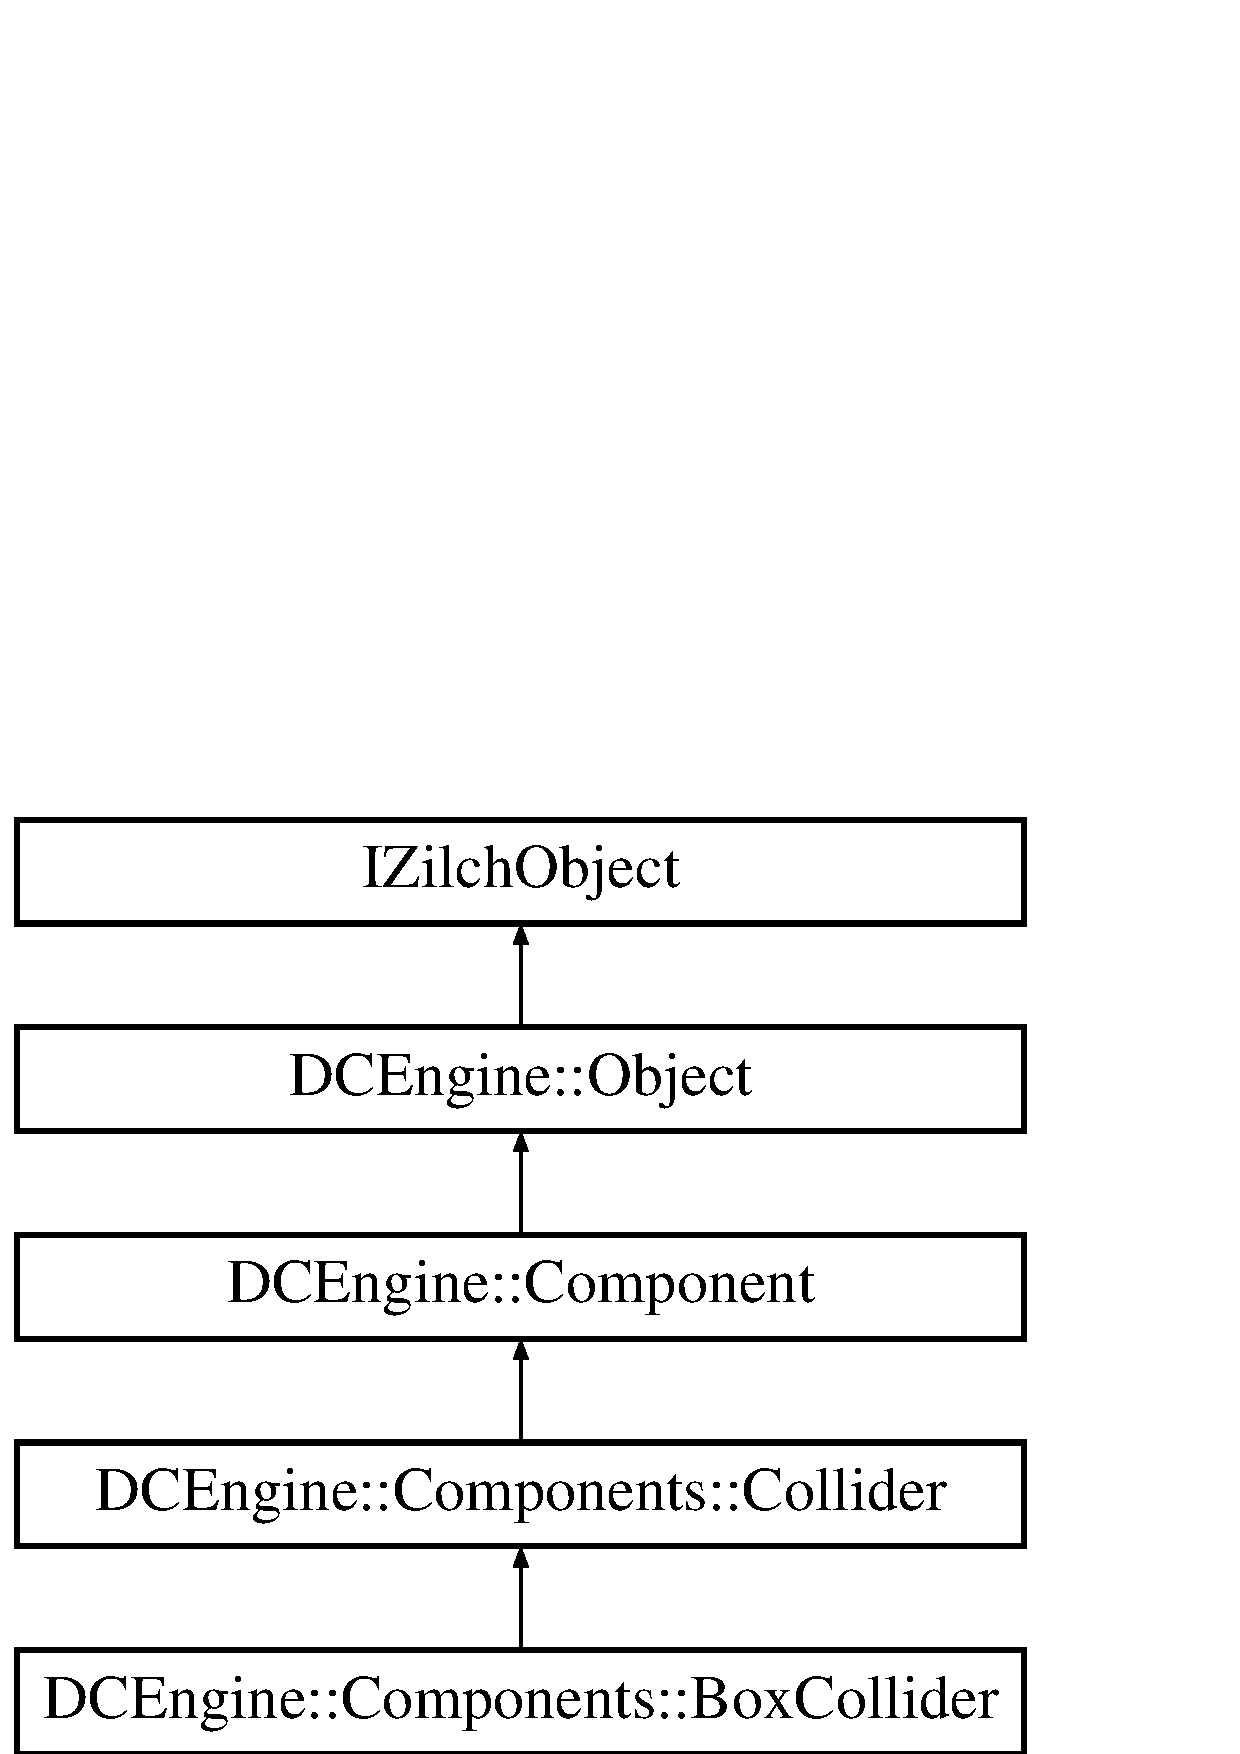
\includegraphics[height=5.000000cm]{classDCEngine_1_1Components_1_1BoxCollider}
\end{center}
\end{figure}
\subsection*{Public Member Functions}
\begin{DoxyCompactItemize}
\item 
\hypertarget{classDCEngine_1_1Components_1_1BoxCollider_a307a276bd1efb29731cd1e6ab8234381}{{\bfseries Zilch\-Declare\-Derived\-Type} (\hyperlink{classDCEngine_1_1Components_1_1BoxCollider}{Box\-Collider}, \hyperlink{classDCEngine_1_1Components_1_1Collider}{Collider})}\label{classDCEngine_1_1Components_1_1BoxCollider_a307a276bd1efb29731cd1e6ab8234381}

\item 
\hypertarget{classDCEngine_1_1Components_1_1BoxCollider_a9ef080e6ea657589e6b0c5dcff467bad}{{\bfseries D\-C\-E\-\_\-\-D\-E\-F\-I\-N\-E\-\_\-\-P\-R\-O\-P\-E\-R\-T\-Y} (Vec3, Size)}\label{classDCEngine_1_1Components_1_1BoxCollider_a9ef080e6ea657589e6b0c5dcff467bad}

\item 
\hypertarget{classDCEngine_1_1Components_1_1BoxCollider_ac58ada13086efa016c4b0e22766acc6c}{{\bfseries D\-C\-E\-\_\-\-D\-E\-F\-I\-N\-E\-\_\-\-P\-R\-O\-P\-E\-R\-T\-Y} (Vec3, Offset)}\label{classDCEngine_1_1Components_1_1BoxCollider_ac58ada13086efa016c4b0e22766acc6c}

\item 
\hypertarget{classDCEngine_1_1Components_1_1BoxCollider_a292c0ad46d3c02aee5eff549be6db3e6}{{\bfseries D\-C\-E\-\_\-\-D\-E\-F\-I\-N\-E\-\_\-\-P\-R\-O\-P\-E\-R\-T\-Y} (Boolean, Ghost)}\label{classDCEngine_1_1Components_1_1BoxCollider_a292c0ad46d3c02aee5eff549be6db3e6}

\item 
\hypertarget{classDCEngine_1_1Components_1_1BoxCollider_a366fa7cdb6f591cf99034d2450002657}{{\bfseries D\-C\-E\-\_\-\-D\-E\-F\-I\-N\-E\-\_\-\-P\-R\-O\-P\-E\-R\-T\-Y} (Boolean, Sends\-Events)}\label{classDCEngine_1_1Components_1_1BoxCollider_a366fa7cdb6f591cf99034d2450002657}

\item 
\hypertarget{classDCEngine_1_1Components_1_1BoxCollider_a15aec7971b17486617b45a032f2e279b}{{\bfseries D\-C\-E\-\_\-\-D\-E\-F\-I\-N\-E\-\_\-\-P\-R\-O\-P\-E\-R\-T\-Y} (Boolean, Is\-Drawing\-Collider)}\label{classDCEngine_1_1Components_1_1BoxCollider_a15aec7971b17486617b45a032f2e279b}

\item 
\hypertarget{classDCEngine_1_1Components_1_1BoxCollider_a21faa64bc4ebcf53b59b3ac7571c0333}{{\bfseries D\-C\-E\-\_\-\-D\-E\-F\-I\-N\-E\-\_\-\-P\-R\-O\-P\-E\-R\-T\-Y} (Collision\-Group\-Handle, \hyperlink{classDCEngine_1_1CollisionGroup}{Collision\-Group})}\label{classDCEngine_1_1Components_1_1BoxCollider_a21faa64bc4ebcf53b59b3ac7571c0333}

\item 
\hypertarget{classDCEngine_1_1Components_1_1BoxCollider_a17f316dd11005453ab43a60f0fef8631}{{\bfseries D\-C\-E\-\_\-\-D\-E\-F\-I\-N\-E\-\_\-\-P\-R\-O\-P\-E\-R\-T\-Y} (Physics\-Material\-Handle, \hyperlink{classDCEngine_1_1PhysicsMaterial}{Physics\-Material})}\label{classDCEngine_1_1Components_1_1BoxCollider_a17f316dd11005453ab43a60f0fef8631}

\item 
\hyperlink{classDCEngine_1_1Components_1_1BoxCollider_a4a0c74f19d98ae6e7f8fabda9c27ae7f}{Box\-Collider} (\hyperlink{classDCEngine_1_1Entity}{Entity} \&owner)
\begin{DoxyCompactList}\small\item\em \hyperlink{classDCEngine_1_1Components_1_1BoxCollider}{Box\-Collider} constructor. \end{DoxyCompactList}\item 
\hypertarget{classDCEngine_1_1Components_1_1BoxCollider_a7dded57707b25afe86b8682cf75685ae}{\hyperlink{classDCEngine_1_1Components_1_1BoxCollider_a7dded57707b25afe86b8682cf75685ae}{$\sim$\-Box\-Collider} ()}\label{classDCEngine_1_1Components_1_1BoxCollider_a7dded57707b25afe86b8682cf75685ae}

\begin{DoxyCompactList}\small\item\em \hyperlink{classDCEngine_1_1Components_1_1BoxCollider}{Box\-Collider} destructor. \end{DoxyCompactList}\item 
\hypertarget{classDCEngine_1_1Components_1_1BoxCollider_a09d8d301ee2e4c210dc7a57f5446441c}{void \hyperlink{classDCEngine_1_1Components_1_1BoxCollider_a09d8d301ee2e4c210dc7a57f5446441c}{Initialize} ()}\label{classDCEngine_1_1Components_1_1BoxCollider_a09d8d301ee2e4c210dc7a57f5446441c}

\begin{DoxyCompactList}\small\item\em Initializes the \hyperlink{classDCEngine_1_1Components_1_1BoxCollider}{Box\-Collider} component. \end{DoxyCompactList}\item 
Vec3 \hyperlink{classDCEngine_1_1Components_1_1BoxCollider_a09020ab4374fdfdd670d0ec788e1dd56}{get\-Collider\-Scale} ()
\begin{DoxyCompactList}\small\item\em \hyperlink{classThe}{The} true scale of the collider is the size set times the scale of the component. \end{DoxyCompactList}\end{DoxyCompactItemize}
\subsection*{Public Attributes}
\begin{DoxyCompactItemize}
\item 
\hypertarget{classDCEngine_1_1Components_1_1BoxCollider_a9de2348be8a6bcd6f61a2e711ecdd0eb}{Vec3 {\bfseries Size} = Vec3(1, 1, 1)}\label{classDCEngine_1_1Components_1_1BoxCollider_a9de2348be8a6bcd6f61a2e711ecdd0eb}

\item 
\hypertarget{classDCEngine_1_1Components_1_1BoxCollider_a8d97e25a0480b3c348dd573f81780bfc}{Vec3 {\bfseries Offset} = Vec3(0, 0, 0)}\label{classDCEngine_1_1Components_1_1BoxCollider_a8d97e25a0480b3c348dd573f81780bfc}

\item 
\hypertarget{classDCEngine_1_1Components_1_1BoxCollider_ab91d66d55512be9e6e3ae67ebe32a85b}{Boolean {\bfseries Ghost} = false}\label{classDCEngine_1_1Components_1_1BoxCollider_ab91d66d55512be9e6e3ae67ebe32a85b}

\item 
\hypertarget{classDCEngine_1_1Components_1_1BoxCollider_a45cda38d0f526fd15f44ef7b7b9ef0f1}{Boolean {\bfseries Sends\-Events} = true}\label{classDCEngine_1_1Components_1_1BoxCollider_a45cda38d0f526fd15f44ef7b7b9ef0f1}

\item 
\hypertarget{classDCEngine_1_1Components_1_1BoxCollider_a4a3c69f9d52283cd3589525af61bef4f}{Boolean {\bfseries Is\-Drawing\-Collider} = false}\label{classDCEngine_1_1Components_1_1BoxCollider_a4a3c69f9d52283cd3589525af61bef4f}

\end{DoxyCompactItemize}
\subsection*{Friends}
\begin{DoxyCompactItemize}
\item 
\hypertarget{classDCEngine_1_1Components_1_1BoxCollider_a2bfcbae6c8e1d7af93c5ac1200b1535c}{class {\bfseries Physics}}\label{classDCEngine_1_1Components_1_1BoxCollider_a2bfcbae6c8e1d7af93c5ac1200b1535c}

\end{DoxyCompactItemize}
\subsection*{Additional Inherited Members}


\subsection{Constructor \& Destructor Documentation}
\hypertarget{classDCEngine_1_1Components_1_1BoxCollider_a4a0c74f19d98ae6e7f8fabda9c27ae7f}{\index{D\-C\-Engine\-::\-Components\-::\-Box\-Collider@{D\-C\-Engine\-::\-Components\-::\-Box\-Collider}!Box\-Collider@{Box\-Collider}}
\index{Box\-Collider@{Box\-Collider}!DCEngine::Components::BoxCollider@{D\-C\-Engine\-::\-Components\-::\-Box\-Collider}}
\subsubsection[{Box\-Collider}]{\setlength{\rightskip}{0pt plus 5cm}D\-C\-Engine\-::\-Components\-::\-Box\-Collider\-::\-Box\-Collider (
\begin{DoxyParamCaption}
\item[{{\bf Entity} \&}]{owner}
\end{DoxyParamCaption}
)}}\label{classDCEngine_1_1Components_1_1BoxCollider_a4a0c74f19d98ae6e7f8fabda9c27ae7f}


\hyperlink{classDCEngine_1_1Components_1_1BoxCollider}{Box\-Collider} constructor. 


\begin{DoxyParams}{Parameters}
{\em owner} & \hyperlink{classA}{A} reference to this component's owner. \\
\hline
\end{DoxyParams}


\subsection{Member Function Documentation}
\hypertarget{classDCEngine_1_1Components_1_1BoxCollider_a09020ab4374fdfdd670d0ec788e1dd56}{\index{D\-C\-Engine\-::\-Components\-::\-Box\-Collider@{D\-C\-Engine\-::\-Components\-::\-Box\-Collider}!get\-Collider\-Scale@{get\-Collider\-Scale}}
\index{get\-Collider\-Scale@{get\-Collider\-Scale}!DCEngine::Components::BoxCollider@{D\-C\-Engine\-::\-Components\-::\-Box\-Collider}}
\subsubsection[{get\-Collider\-Scale}]{\setlength{\rightskip}{0pt plus 5cm}Vec3 D\-C\-Engine\-::\-Components\-::\-Box\-Collider\-::get\-Collider\-Scale (
\begin{DoxyParamCaption}
{}
\end{DoxyParamCaption}
)}}\label{classDCEngine_1_1Components_1_1BoxCollider_a09020ab4374fdfdd670d0ec788e1dd56}


\hyperlink{classThe}{The} true scale of the collider is the size set times the scale of the component. 

\begin{DoxyNote}{Note}
So if an object's transform scale was set at 1 while the collider's size was set at 2, the collider would be twice the size of the object. 
\end{DoxyNote}


The documentation for this class was generated from the following files\-:\begin{DoxyCompactItemize}
\item 
Core/\-Components/\hyperlink{BoxCollider_8h}{Box\-Collider.\-h}\item 
Core/\-Components/\hyperlink{BoxCollider_8cpp}{Box\-Collider.\-cpp}\end{DoxyCompactItemize}

\hypertarget{classDCEngine_1_1Components_1_1Button}{\section{D\-C\-Engine\-:\-:Components\-:\-:Button Class Reference}
\label{classDCEngine_1_1Components_1_1Button}\index{D\-C\-Engine\-::\-Components\-::\-Button@{D\-C\-Engine\-::\-Components\-::\-Button}}
}
Inheritance diagram for D\-C\-Engine\-:\-:Components\-:\-:Button\-:\begin{figure}[H]
\begin{center}
\leavevmode
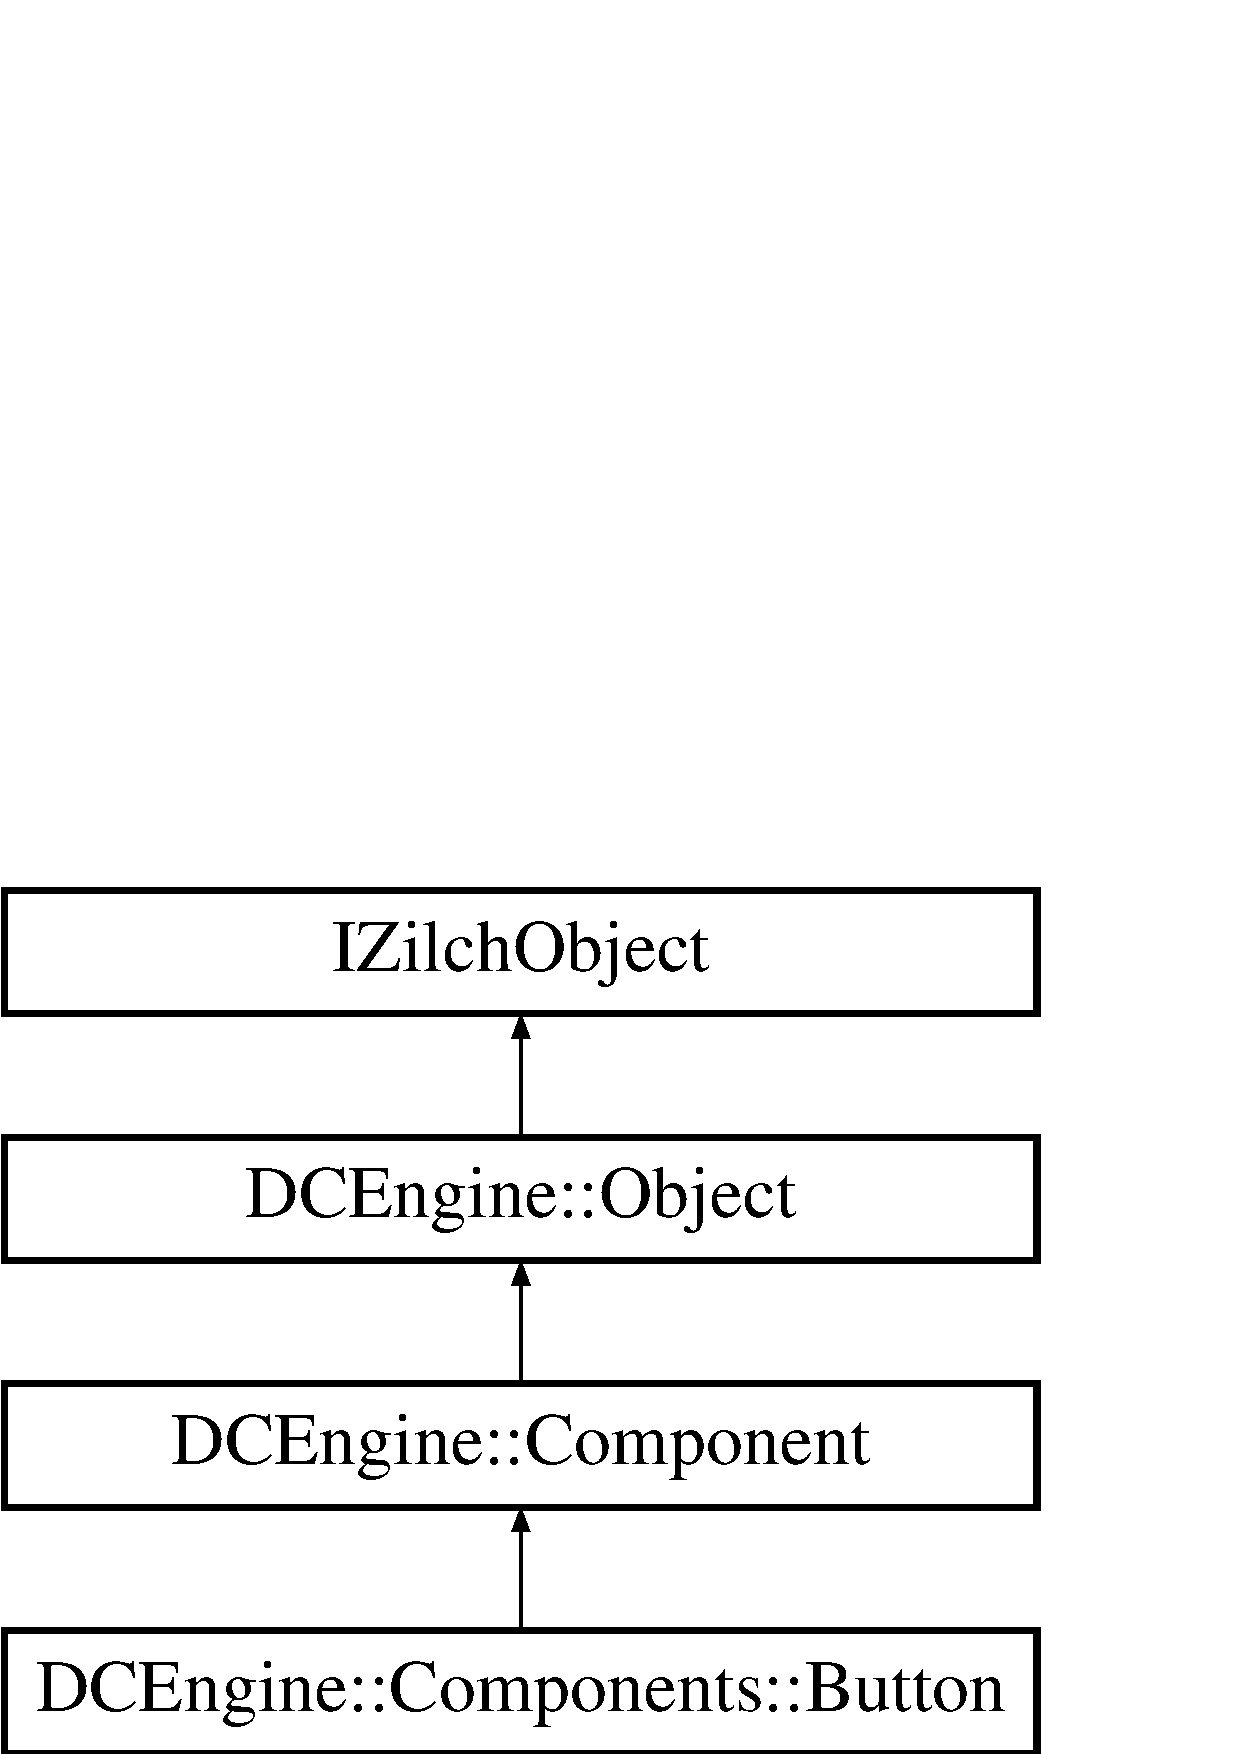
\includegraphics[height=4.000000cm]{classDCEngine_1_1Components_1_1Button}
\end{center}
\end{figure}
\subsection*{Public Member Functions}
\begin{DoxyCompactItemize}
\item 
\hypertarget{classDCEngine_1_1Components_1_1Button_adda83c8f6f6f505fad15e0dd43acc5d3}{{\bfseries D\-C\-E\-\_\-\-D\-E\-F\-I\-N\-E\-\_\-\-P\-R\-O\-P\-E\-R\-T\-Y} (String, Target)}\label{classDCEngine_1_1Components_1_1Button_adda83c8f6f6f505fad15e0dd43acc5d3}

\item 
\hypertarget{classDCEngine_1_1Components_1_1Button_a468edecec2570f7cd69eb2d283c280d1}{{\bfseries Button} (\hyperlink{classDCEngine_1_1Entity}{Entity} \&owner)}\label{classDCEngine_1_1Components_1_1Button_a468edecec2570f7cd69eb2d283c280d1}

\item 
\hypertarget{classDCEngine_1_1Components_1_1Button_a1928a37df78c5c8f5f40f042838a8d65}{void {\bfseries Initialize} ()}\label{classDCEngine_1_1Components_1_1Button_a1928a37df78c5c8f5f40f042838a8d65}

\item 
\hypertarget{classDCEngine_1_1Components_1_1Button_ad37fcf19a03509021804b68735066e85}{void {\bfseries On\-Mouse\-Down\-Event} (\hyperlink{classDCEngine_1_1Events_1_1MouseDown}{Events\-::\-Mouse\-Down} $\ast$event)}\label{classDCEngine_1_1Components_1_1Button_ad37fcf19a03509021804b68735066e85}

\item 
\hypertarget{classDCEngine_1_1Components_1_1Button_a9b2a12675f2f4393c025dab4dffadfef}{void {\bfseries On\-Mouse\-Up\-Event} (\hyperlink{classDCEngine_1_1Events_1_1MouseUp}{Events\-::\-Mouse\-Up} $\ast$event)}\label{classDCEngine_1_1Components_1_1Button_a9b2a12675f2f4393c025dab4dffadfef}

\item 
\hypertarget{classDCEngine_1_1Components_1_1Button_a0aee8944548eb3fe1f1d633887d10b48}{void {\bfseries On\-Key\-Down\-Event} (\hyperlink{classDCEngine_1_1Events_1_1KeyDown}{Events\-::\-Key\-Down} $\ast$event)}\label{classDCEngine_1_1Components_1_1Button_a0aee8944548eb3fe1f1d633887d10b48}

\item 
\hypertarget{classDCEngine_1_1Components_1_1Button_a71717f0bd769c2e2fcad8eddf1422439}{void {\bfseries On\-Key\-Up\-Event} (\hyperlink{classDCEngine_1_1Events_1_1KeyDown}{Events\-::\-Key\-Down} $\ast$event)}\label{classDCEngine_1_1Components_1_1Button_a71717f0bd769c2e2fcad8eddf1422439}

\item 
\hypertarget{classDCEngine_1_1Components_1_1Button_ad28a27adf0fda22a79781859fc32eda9}{void {\bfseries On\-Collision\-Started\-Event} (\hyperlink{classDCEngine_1_1Events_1_1CollisionStarted}{Events\-::\-Collision\-Started} $\ast$event)}\label{classDCEngine_1_1Components_1_1Button_ad28a27adf0fda22a79781859fc32eda9}

\item 
\hypertarget{classDCEngine_1_1Components_1_1Button_a2c65d37f08b7ab3292b23ef300fd4eeb}{void {\bfseries On\-Collision\-Ended\-Event} (\hyperlink{classDCEngine_1_1Events_1_1CollisionEnded}{Events\-::\-Collision\-Ended} $\ast$event)}\label{classDCEngine_1_1Components_1_1Button_a2c65d37f08b7ab3292b23ef300fd4eeb}

\item 
\hypertarget{classDCEngine_1_1Components_1_1Button_a3a6d3791339f69321c6bf6cbda03fc70}{void {\bfseries On\-Logic\-Update\-Event} (\hyperlink{classDCEngine_1_1Events_1_1LogicUpdate}{Events\-::\-Logic\-Update} $\ast$event)}\label{classDCEngine_1_1Components_1_1Button_a3a6d3791339f69321c6bf6cbda03fc70}

\item 
\hypertarget{classDCEngine_1_1Components_1_1Button_a4ef28054684c02f68ddcdcf4e31ac28b}{{\bfseries Zilch\-Declare\-Derived\-Type} (\hyperlink{classDCEngine_1_1Components_1_1Button}{Button}, \hyperlink{classDCEngine_1_1Component}{Component})}\label{classDCEngine_1_1Components_1_1Button_a4ef28054684c02f68ddcdcf4e31ac28b}

\end{DoxyCompactItemize}
\subsection*{Public Attributes}
\begin{DoxyCompactItemize}
\item 
\hypertarget{classDCEngine_1_1Components_1_1Button_a58d17b4572b2bb516ded2dec0460a62e}{\hyperlink{classDCEngine_1_1Components_1_1Transform}{Transform} $\ast$ {\bfseries Transform\-Ref}}\label{classDCEngine_1_1Components_1_1Button_a58d17b4572b2bb516ded2dec0460a62e}

\item 
\hypertarget{classDCEngine_1_1Components_1_1Button_a7f4f78d9e401f04221e35caa94e59693}{\hyperlink{classDCEngine_1_1Components_1_1Sprite}{Sprite} $\ast$ {\bfseries Sprite\-Ref}}\label{classDCEngine_1_1Components_1_1Button_a7f4f78d9e401f04221e35caa94e59693}

\end{DoxyCompactItemize}
\subsection*{Additional Inherited Members}


The documentation for this class was generated from the following files\-:\begin{DoxyCompactItemize}
\item 
Projects/\-Rebound/\-Components/\hyperlink{Button_8h}{Button.\-h}\item 
Projects/\-Rebound/\-Components/\hyperlink{Button_8cpp}{Button.\-cpp}\end{DoxyCompactItemize}

\hypertarget{classDCEngine_1_1Components_1_1Camera}{\section{D\-C\-Engine\-:\-:Components\-:\-:Camera Class Reference}
\label{classDCEngine_1_1Components_1_1Camera}\index{D\-C\-Engine\-::\-Components\-::\-Camera@{D\-C\-Engine\-::\-Components\-::\-Camera}}
}
Inheritance diagram for D\-C\-Engine\-:\-:Components\-:\-:Camera\-:\begin{figure}[H]
\begin{center}
\leavevmode
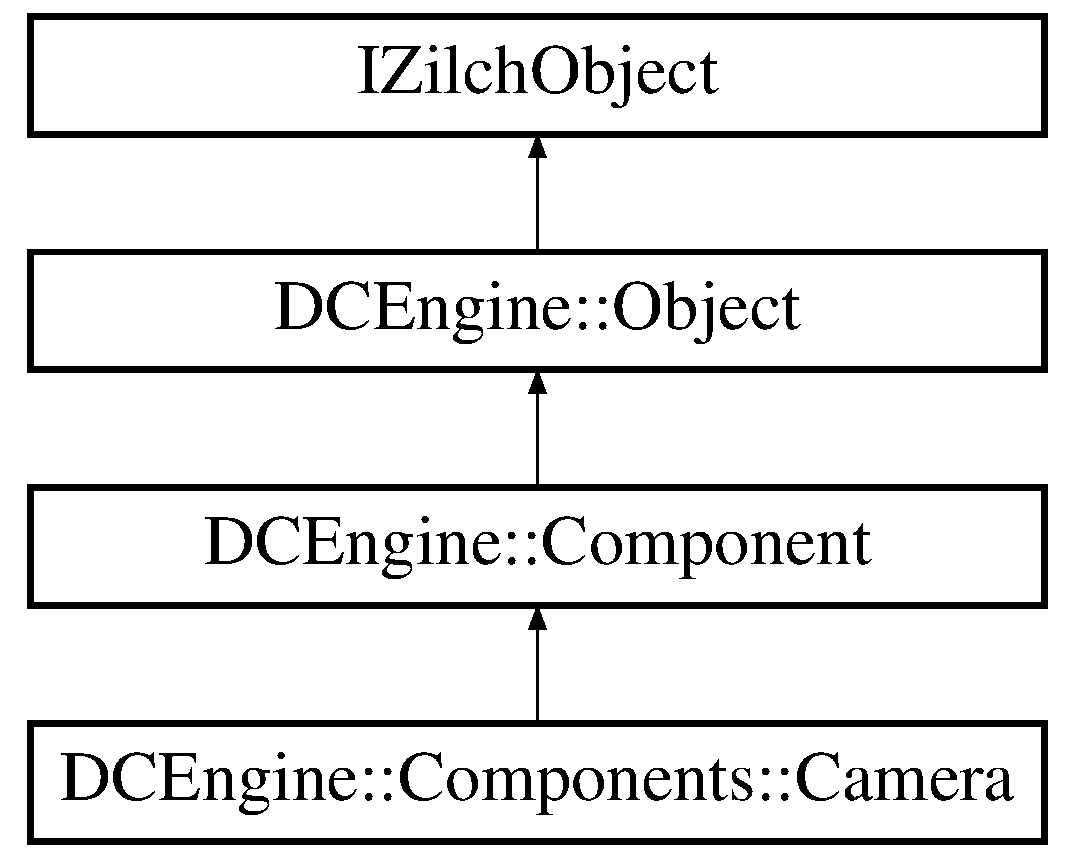
\includegraphics[height=4.000000cm]{classDCEngine_1_1Components_1_1Camera}
\end{center}
\end{figure}
\subsection*{Public Member Functions}
\begin{DoxyCompactItemize}
\item 
\hypertarget{classDCEngine_1_1Components_1_1Camera_ab1f8f7578addf35b6a55fd0ac8e4d9e1}{{\bfseries Zilch\-Declare\-Derived\-Type} (\hyperlink{classDCEngine_1_1Components_1_1Camera}{Camera}, \hyperlink{classDCEngine_1_1Component}{Component})}\label{classDCEngine_1_1Components_1_1Camera_ab1f8f7578addf35b6a55fd0ac8e4d9e1}

\item 
\hypertarget{classDCEngine_1_1Components_1_1Camera_ac7918d0075ae3b6a916ff44df0037128}{Real {\bfseries get\-Field\-Of\-View} () const }\label{classDCEngine_1_1Components_1_1Camera_ac7918d0075ae3b6a916ff44df0037128}

\item 
\hypertarget{classDCEngine_1_1Components_1_1Camera_a72c0a86f03f7da3ec74a1cfa5162ba8e}{void {\bfseries set\-Field\-Of\-View} (Real)}\label{classDCEngine_1_1Components_1_1Camera_a72c0a86f03f7da3ec74a1cfa5162ba8e}

\item 
\hypertarget{classDCEngine_1_1Components_1_1Camera_a7d048811a5bcf85c1b9b9a59ea20855c}{Real {\bfseries get\-Near\-Plane} () const }\label{classDCEngine_1_1Components_1_1Camera_a7d048811a5bcf85c1b9b9a59ea20855c}

\item 
\hypertarget{classDCEngine_1_1Components_1_1Camera_ac751387f7e27d0ec86752e2737242823}{void {\bfseries set\-Near\-Plane} (Real)}\label{classDCEngine_1_1Components_1_1Camera_ac751387f7e27d0ec86752e2737242823}

\item 
\hypertarget{classDCEngine_1_1Components_1_1Camera_a01f023f9d44a0a5a117a261384c481fc}{Real {\bfseries get\-Far\-Plane} () const }\label{classDCEngine_1_1Components_1_1Camera_a01f023f9d44a0a5a117a261384c481fc}

\item 
\hypertarget{classDCEngine_1_1Components_1_1Camera_a813522c95cfbd66911da43d94bbd0a5f}{void {\bfseries set\-Far\-Plane} (Real)}\label{classDCEngine_1_1Components_1_1Camera_a813522c95cfbd66911da43d94bbd0a5f}

\item 
\hypertarget{classDCEngine_1_1Components_1_1Camera_a53dee4bd5006d11eb5ea888875cd1cb3}{Real {\bfseries get\-Size} () const }\label{classDCEngine_1_1Components_1_1Camera_a53dee4bd5006d11eb5ea888875cd1cb3}

\item 
\hypertarget{classDCEngine_1_1Components_1_1Camera_ad668eb9422ed01c2f56ec63bccecaeaa}{void {\bfseries set\-Size} (Real)}\label{classDCEngine_1_1Components_1_1Camera_ad668eb9422ed01c2f56ec63bccecaeaa}

\item 
\hypertarget{classDCEngine_1_1Components_1_1Camera_af93426305069908f684de8bde576dd17}{{\bfseries D\-C\-E\-\_\-\-D\-E\-F\-I\-N\-E\-\_\-\-P\-R\-O\-P\-E\-R\-T\-Y} (bool, Active)}\label{classDCEngine_1_1Components_1_1Camera_af93426305069908f684de8bde576dd17}

\item 
\hypertarget{classDCEngine_1_1Components_1_1Camera_abec61d44be812cf153c7156666f6a430}{{\bfseries D\-C\-E\-\_\-\-D\-E\-F\-I\-N\-E\-\_\-\-P\-R\-O\-P\-E\-R\-T\-Y} (Projection\-Mode, Projection)}\label{classDCEngine_1_1Components_1_1Camera_abec61d44be812cf153c7156666f6a430}

\item 
\hypertarget{classDCEngine_1_1Components_1_1Camera_ad09d6ebd5e78940ad608e7fe7cf9d935}{glm\-::mat4 {\bfseries Get\-View\-Matrix} ()}\label{classDCEngine_1_1Components_1_1Camera_ad09d6ebd5e78940ad608e7fe7cf9d935}

\item 
\hypertarget{classDCEngine_1_1Components_1_1Camera_a2cf5053654219b9922c7b5d7e9659475}{glm\-::mat4 {\bfseries Get\-Projection\-Matrix} ()}\label{classDCEngine_1_1Components_1_1Camera_a2cf5053654219b9922c7b5d7e9659475}

\item 
\hypertarget{classDCEngine_1_1Components_1_1Camera_aea7f55eb0839fcf5ab3e916b0a322cc5}{{\bfseries Camera} (\hyperlink{classDCEngine_1_1Entity}{Entity} \&owner)}\label{classDCEngine_1_1Components_1_1Camera_aea7f55eb0839fcf5ab3e916b0a322cc5}

\item 
\hypertarget{classDCEngine_1_1Components_1_1Camera_a0defeac595a9c8a5d4f9b8a56dd9415d}{void {\bfseries Initialize} ()}\label{classDCEngine_1_1Components_1_1Camera_a0defeac595a9c8a5d4f9b8a56dd9415d}

\item 
\hypertarget{classDCEngine_1_1Components_1_1Camera_ab108d1e0071ec1c3a9483cbb7f1731e5}{void {\bfseries On\-Logic\-Update} (\hyperlink{classDCEngine_1_1Events_1_1LogicUpdate}{Events\-::\-Logic\-Update} $\ast$event)}\label{classDCEngine_1_1Components_1_1Camera_ab108d1e0071ec1c3a9483cbb7f1731e5}

\end{DoxyCompactItemize}
\subsection*{Public Attributes}
\begin{DoxyCompactItemize}
\item 
\hypertarget{classDCEngine_1_1Components_1_1Camera_acf10f0b7b422b9c069c9ba8cacf0142b}{glm\-::vec3 {\bfseries Front} = glm\-::vec3(0.\-0f, 0.\-0f, -\/1.\-0f)}\label{classDCEngine_1_1Components_1_1Camera_acf10f0b7b422b9c069c9ba8cacf0142b}

\item 
\hypertarget{classDCEngine_1_1Components_1_1Camera_ad4f21f54c25e04d55cdb3c84072c1a96}{glm\-::vec3 {\bfseries Up} = glm\-::vec3(0.\-0f, 1.\-0f, 0.\-0f)}\label{classDCEngine_1_1Components_1_1Camera_ad4f21f54c25e04d55cdb3c84072c1a96}

\item 
\hypertarget{classDCEngine_1_1Components_1_1Camera_a7c2007cccce80e9ab55d575dad8157e6}{glm\-::vec3 {\bfseries Right} = glm\-::vec3(1.\-0f, 0.\-0f, 0.\-0f)}\label{classDCEngine_1_1Components_1_1Camera_a7c2007cccce80e9ab55d575dad8157e6}

\item 
\hypertarget{classDCEngine_1_1Components_1_1Camera_a564d09b431ddf2bbf0baf5312af9dd24}{G\-Lfloat {\bfseries Yaw} = 90.\-0f}\label{classDCEngine_1_1Components_1_1Camera_a564d09b431ddf2bbf0baf5312af9dd24}

\item 
\hypertarget{classDCEngine_1_1Components_1_1Camera_ae2c529610eb6615f0c99db94e20608d5}{G\-Lfloat {\bfseries Pitch} = 0.\-0f}\label{classDCEngine_1_1Components_1_1Camera_ae2c529610eb6615f0c99db94e20608d5}

\item 
\hypertarget{classDCEngine_1_1Components_1_1Camera_a9c0cf62f2fc6f53dcd0285cc63330383}{G\-Lfloat {\bfseries Roll} = 90.\-0f}\label{classDCEngine_1_1Components_1_1Camera_a9c0cf62f2fc6f53dcd0285cc63330383}

\item 
\hypertarget{classDCEngine_1_1Components_1_1Camera_a3a0ee4b6b5fed69e1581a86df8a8ff22}{G\-Lfloat {\bfseries Base\-Roll\-Val} = 90.\-0f}\label{classDCEngine_1_1Components_1_1Camera_a3a0ee4b6b5fed69e1581a86df8a8ff22}

\item 
\hypertarget{classDCEngine_1_1Components_1_1Camera_a80403f32c67b2d3a3bb1a7ab0ba9e97a}{Projection\-Mode {\bfseries Projection} = Projection\-Mode\-::\-Perspective}\label{classDCEngine_1_1Components_1_1Camera_a80403f32c67b2d3a3bb1a7ab0ba9e97a}

\item 
\hypertarget{classDCEngine_1_1Components_1_1Camera_ae39daf64c16eed8722b06b3f298f59b2}{G\-Lfloat {\bfseries Field\-Of\-View} = 250}\label{classDCEngine_1_1Components_1_1Camera_ae39daf64c16eed8722b06b3f298f59b2}

\item 
\hypertarget{classDCEngine_1_1Components_1_1Camera_afce6a46766da72932e4c520ba5819a41}{G\-Lfloat {\bfseries Window\-Width} = 8}\label{classDCEngine_1_1Components_1_1Camera_afce6a46766da72932e4c520ba5819a41}

\item 
\hypertarget{classDCEngine_1_1Components_1_1Camera_a50aa6cd802041e51dfa588489e345662}{G\-Lfloat {\bfseries Window\-Height} = 6}\label{classDCEngine_1_1Components_1_1Camera_a50aa6cd802041e51dfa588489e345662}

\item 
\hypertarget{classDCEngine_1_1Components_1_1Camera_a1a2cdf44bfe50f5c29af04ae084beb17}{G\-Lfloat {\bfseries Size} = 90}\label{classDCEngine_1_1Components_1_1Camera_a1a2cdf44bfe50f5c29af04ae084beb17}

\item 
\hypertarget{classDCEngine_1_1Components_1_1Camera_a964822aa1b2029bacd469e59a00b97d3}{G\-Lfloat {\bfseries Near\-Plane} = 0.\-1f}\label{classDCEngine_1_1Components_1_1Camera_a964822aa1b2029bacd469e59a00b97d3}

\item 
\hypertarget{classDCEngine_1_1Components_1_1Camera_abb5fb7e37ffd7ae9df6f5163732b8f27}{G\-Lfloat {\bfseries Far\-Plane} = 100.\-0f}\label{classDCEngine_1_1Components_1_1Camera_abb5fb7e37ffd7ae9df6f5163732b8f27}

\item 
\hypertarget{classDCEngine_1_1Components_1_1Camera_ae433fad9d7fba93fa411d0999882602c}{\hyperlink{classDCEngine_1_1Components_1_1Transform}{Transform} $\ast$ {\bfseries Transform\-Component}}\label{classDCEngine_1_1Components_1_1Camera_ae433fad9d7fba93fa411d0999882602c}

\end{DoxyCompactItemize}
\subsection*{Friends}
\begin{DoxyCompactItemize}
\item 
\hypertarget{classDCEngine_1_1Components_1_1Camera_a9634ae1550d5c7bd5b7cc67eb933ec91}{class {\bfseries Camera\-Viewport}}\label{classDCEngine_1_1Components_1_1Camera_a9634ae1550d5c7bd5b7cc67eb933ec91}

\end{DoxyCompactItemize}
\subsection*{Additional Inherited Members}


The documentation for this class was generated from the following file\-:\begin{DoxyCompactItemize}
\item 
Core/\-Components/\hyperlink{Camera_8h}{Camera.\-h}\end{DoxyCompactItemize}

\hypertarget{classDCEngine_1_1Components_1_1CameraController}{\section{D\-C\-Engine\-:\-:Components\-:\-:Camera\-Controller Class Reference}
\label{classDCEngine_1_1Components_1_1CameraController}\index{D\-C\-Engine\-::\-Components\-::\-Camera\-Controller@{D\-C\-Engine\-::\-Components\-::\-Camera\-Controller}}
}
Inheritance diagram for D\-C\-Engine\-:\-:Components\-:\-:Camera\-Controller\-:\begin{figure}[H]
\begin{center}
\leavevmode
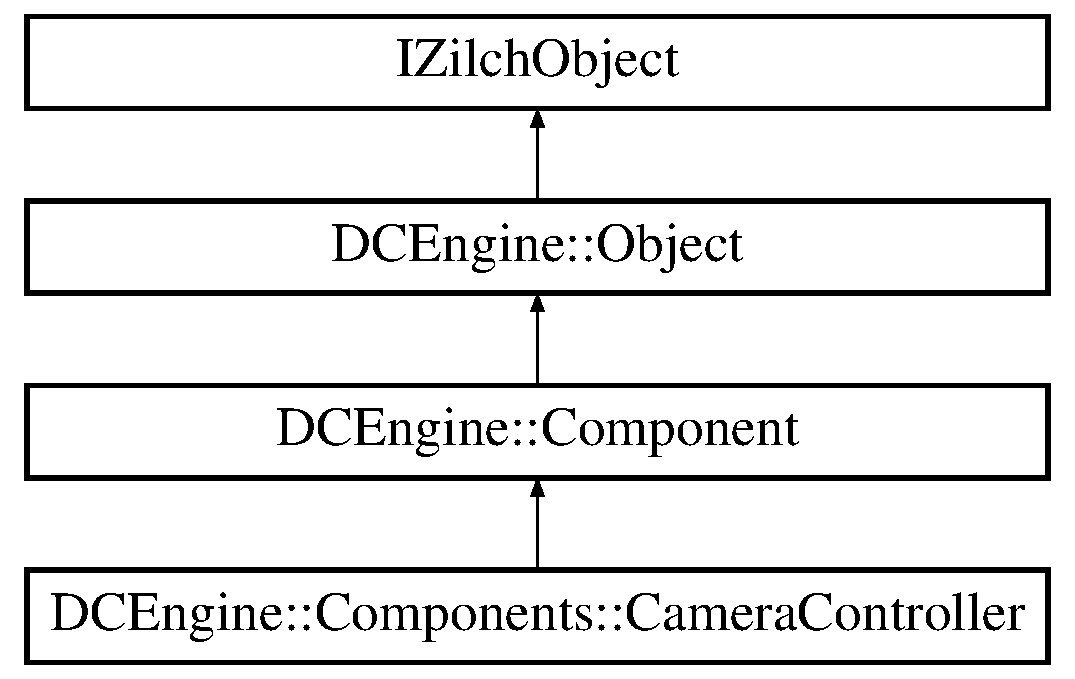
\includegraphics[height=4.000000cm]{classDCEngine_1_1Components_1_1CameraController}
\end{center}
\end{figure}
\subsection*{Public Member Functions}
\begin{DoxyCompactItemize}
\item 
\hypertarget{classDCEngine_1_1Components_1_1CameraController_aa5cf9a4a9100bd552f5d06ae88580552}{{\bfseries D\-C\-E\-\_\-\-D\-E\-F\-I\-N\-E\-\_\-\-P\-R\-O\-P\-E\-R\-T\-Y} (String, Target\-Name)}\label{classDCEngine_1_1Components_1_1CameraController_aa5cf9a4a9100bd552f5d06ae88580552}

\item 
\hypertarget{classDCEngine_1_1Components_1_1CameraController_ac5b7383968adc711f02c972920a6e67b}{{\bfseries D\-C\-E\-\_\-\-D\-E\-F\-I\-N\-E\-\_\-\-P\-R\-O\-P\-E\-R\-T\-Y} (Real, Interpolation\-Speed)}\label{classDCEngine_1_1Components_1_1CameraController_ac5b7383968adc711f02c972920a6e67b}

\item 
\hypertarget{classDCEngine_1_1Components_1_1CameraController_a2ca2a5946e5652b44426b1a92284bef2}{{\bfseries Camera\-Controller} (\hyperlink{classDCEngine_1_1Entity}{Entity} \&owner)}\label{classDCEngine_1_1Components_1_1CameraController_a2ca2a5946e5652b44426b1a92284bef2}

\item 
\hypertarget{classDCEngine_1_1Components_1_1CameraController_ac874899f88de6d8516f9e5554270282f}{void {\bfseries Initialize} ()}\label{classDCEngine_1_1Components_1_1CameraController_ac874899f88de6d8516f9e5554270282f}

\item 
\hypertarget{classDCEngine_1_1Components_1_1CameraController_a4ed1fa10e835f7596cb10d361a4dad27}{virtual void {\bfseries Serialize} (Json\-::\-Value \&root)}\label{classDCEngine_1_1Components_1_1CameraController_a4ed1fa10e835f7596cb10d361a4dad27}

\item 
\hypertarget{classDCEngine_1_1Components_1_1CameraController_a3dac551a7dc7e5eb151c896a5cfeb393}{virtual void {\bfseries Deserialize} (Json\-::\-Value \&root)}\label{classDCEngine_1_1Components_1_1CameraController_a3dac551a7dc7e5eb151c896a5cfeb393}

\item 
\hypertarget{classDCEngine_1_1Components_1_1CameraController_aa69a7456ca7f79c08f7e4da9e22ac006}{void {\bfseries On\-Key\-Down\-Event} (\hyperlink{classDCEngine_1_1Events_1_1KeyDown}{Events\-::\-Key\-Down} $\ast$event)}\label{classDCEngine_1_1Components_1_1CameraController_aa69a7456ca7f79c08f7e4da9e22ac006}

\item 
\hypertarget{classDCEngine_1_1Components_1_1CameraController_a26eb53387cff24fe05c901f250c30f71}{void {\bfseries On\-Mouse\-Down\-Event} (\hyperlink{classDCEngine_1_1Events_1_1MouseDown}{Events\-::\-Mouse\-Down} $\ast$event)}\label{classDCEngine_1_1Components_1_1CameraController_a26eb53387cff24fe05c901f250c30f71}

\item 
\hypertarget{classDCEngine_1_1Components_1_1CameraController_a1bd3cb86f86c2e7eae355b7cf052e3f7}{void {\bfseries On\-Mouse\-Up\-Event} (\hyperlink{classDCEngine_1_1Events_1_1MouseUp}{Events\-::\-Mouse\-Up} $\ast$event)}\label{classDCEngine_1_1Components_1_1CameraController_a1bd3cb86f86c2e7eae355b7cf052e3f7}

\item 
\hypertarget{classDCEngine_1_1Components_1_1CameraController_a2fd8ce29a27b7442bf211ae56660bb3e}{void {\bfseries Camera\-Controller\-::\-On\-Logic\-Update\-Event} (\hyperlink{classDCEngine_1_1Events_1_1LogicUpdate}{Events\-::\-Logic\-Update} $\ast$event)}\label{classDCEngine_1_1Components_1_1CameraController_a2fd8ce29a27b7442bf211ae56660bb3e}

\item 
\hypertarget{classDCEngine_1_1Components_1_1CameraController_a989db8de4c40bf142448c073d0c66798}{{\bfseries Zilch\-Declare\-Derived\-Type} (\hyperlink{classDCEngine_1_1Components_1_1CameraController}{Camera\-Controller}, \hyperlink{classDCEngine_1_1Component}{Component})}\label{classDCEngine_1_1Components_1_1CameraController_a989db8de4c40bf142448c073d0c66798}

\end{DoxyCompactItemize}
\subsection*{Public Attributes}
\begin{DoxyCompactItemize}
\item 
\hypertarget{classDCEngine_1_1Components_1_1CameraController_a5190142b41d9a25608c5dc4d5efe1171}{\hyperlink{classDCEngine_1_1Components_1_1Transform}{Transform} $\ast$ {\bfseries Transform\-Ref}}\label{classDCEngine_1_1Components_1_1CameraController_a5190142b41d9a25608c5dc4d5efe1171}

\item 
\hypertarget{classDCEngine_1_1Components_1_1CameraController_a0162002af3f11d7b6245de3f9aa58193}{\hyperlink{classDCEngine_1_1Components_1_1Sprite}{Sprite} $\ast$ {\bfseries Sprite\-Ref}}\label{classDCEngine_1_1Components_1_1CameraController_a0162002af3f11d7b6245de3f9aa58193}

\item 
\hypertarget{classDCEngine_1_1Components_1_1CameraController_ae80025e660b279db751ebcd69d30de18}{\hyperlink{classDCEngine_1_1GameObject}{Game\-Object} $\ast$ {\bfseries Player\-Ref}}\label{classDCEngine_1_1Components_1_1CameraController_ae80025e660b279db751ebcd69d30de18}

\item 
\hypertarget{classDCEngine_1_1Components_1_1CameraController_a7204ad61f0f57addd17b3a1fbeea93c4}{Real {\bfseries Interpolation\-Speed} = 0.\-06f}\label{classDCEngine_1_1Components_1_1CameraController_a7204ad61f0f57addd17b3a1fbeea93c4}

\item 
\hypertarget{classDCEngine_1_1Components_1_1CameraController_a9cee8d024f211e9d863cd6555585504e}{String {\bfseries Target\-Name} = \char`\"{}Player\char`\"{}}\label{classDCEngine_1_1Components_1_1CameraController_a9cee8d024f211e9d863cd6555585504e}

\item 
\hypertarget{classDCEngine_1_1Components_1_1CameraController_ae3a5ee0e7bc89903babb3a5426dd266c}{Boolean {\bfseries Do\-Screen\-Shake} = false}\label{classDCEngine_1_1Components_1_1CameraController_ae3a5ee0e7bc89903babb3a5426dd266c}

\end{DoxyCompactItemize}
\subsection*{Additional Inherited Members}


The documentation for this class was generated from the following files\-:\begin{DoxyCompactItemize}
\item 
Projects/\-Rebound/\-Components/\hyperlink{CameraController_8h}{Camera\-Controller.\-h}\item 
Projects/\-Rebound/\-Components/Camera\-Controller.\-cpp\end{DoxyCompactItemize}

\hypertarget{classDCEngine_1_1Components_1_1CameraViewport}{\section{D\-C\-Engine\-:\-:Components\-:\-:Camera\-Viewport Class Reference}
\label{classDCEngine_1_1Components_1_1CameraViewport}\index{D\-C\-Engine\-::\-Components\-::\-Camera\-Viewport@{D\-C\-Engine\-::\-Components\-::\-Camera\-Viewport}}
}
Inheritance diagram for D\-C\-Engine\-:\-:Components\-:\-:Camera\-Viewport\-:\begin{figure}[H]
\begin{center}
\leavevmode
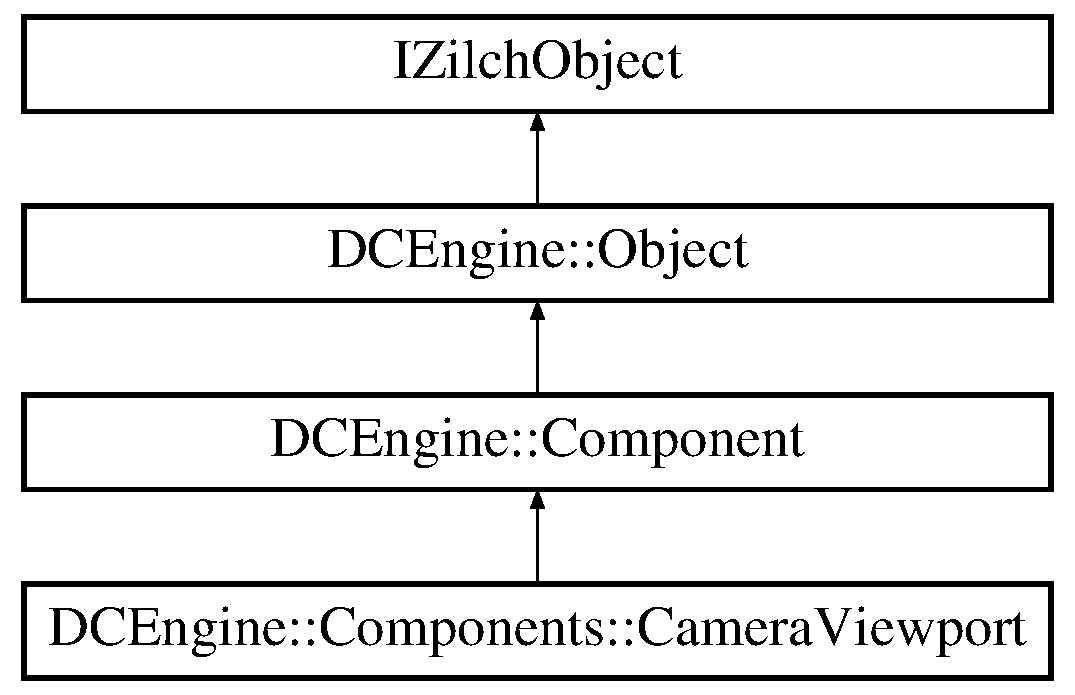
\includegraphics[height=4.000000cm]{classDCEngine_1_1Components_1_1CameraViewport}
\end{center}
\end{figure}
\subsection*{Public Member Functions}
\begin{DoxyCompactItemize}
\item 
\hypertarget{classDCEngine_1_1Components_1_1CameraViewport_ac785b32b12b975406601025a03873cf7}{{\bfseries Zilch\-Declare\-Derived\-Type} (\hyperlink{classDCEngine_1_1Components_1_1CameraViewport}{Camera\-Viewport}, \hyperlink{classDCEngine_1_1Component}{Component})}\label{classDCEngine_1_1Components_1_1CameraViewport_ac785b32b12b975406601025a03873cf7}

\item 
\hypertarget{classDCEngine_1_1Components_1_1CameraViewport_aaa16a851fb8fdf79a15b9bb6fa8727e5}{{\bfseries D\-C\-E\-\_\-\-D\-E\-F\-I\-N\-E\-\_\-\-P\-R\-O\-P\-E\-R\-T\-Y} (bool, Active)}\label{classDCEngine_1_1Components_1_1CameraViewport_aaa16a851fb8fdf79a15b9bb6fa8727e5}

\item 
\hypertarget{classDCEngine_1_1Components_1_1CameraViewport_ac9b944257146988ca9d9137df70f7e19}{{\bfseries D\-C\-E\-\_\-\-D\-E\-F\-I\-N\-E\-\_\-\-P\-R\-O\-P\-E\-R\-T\-Y} (bool, Blocking)}\label{classDCEngine_1_1Components_1_1CameraViewport_ac9b944257146988ca9d9137df70f7e19}

\item 
\hypertarget{classDCEngine_1_1Components_1_1CameraViewport_a45ba6134c2d0cd083317bf9a12f3648a}{{\bfseries D\-C\-E\-\_\-\-D\-E\-F\-I\-N\-E\-\_\-\-P\-R\-O\-P\-E\-R\-T\-Y} (int, Layer)}\label{classDCEngine_1_1Components_1_1CameraViewport_a45ba6134c2d0cd083317bf9a12f3648a}

\item 
\hypertarget{classDCEngine_1_1Components_1_1CameraViewport_a32e88b581c4db5e4b3a852a4b5227daa}{{\bfseries D\-C\-E\-\_\-\-D\-E\-F\-I\-N\-E\-\_\-\-P\-R\-O\-P\-E\-R\-T\-Y} (bool, Background)}\label{classDCEngine_1_1Components_1_1CameraViewport_a32e88b581c4db5e4b3a852a4b5227daa}

\item 
\hypertarget{classDCEngine_1_1Components_1_1CameraViewport_a605ff48a635f807edaeaf1f12a3f1514}{{\bfseries D\-C\-E\-\_\-\-D\-E\-F\-I\-N\-E\-\_\-\-P\-R\-O\-P\-E\-R\-T\-Y} (Vec2, Viewport\-Resolution)}\label{classDCEngine_1_1Components_1_1CameraViewport_a605ff48a635f807edaeaf1f12a3f1514}

\item 
\hypertarget{classDCEngine_1_1Components_1_1CameraViewport_ac022942f3fee38bf3156b9300d325ebf}{Vec3 {\bfseries Screen\-To\-World\-View\-Plane} (Vec2 screen\-Point, float view\-Depth)}\label{classDCEngine_1_1Components_1_1CameraViewport_ac022942f3fee38bf3156b9300d325ebf}

\item 
\hypertarget{classDCEngine_1_1Components_1_1CameraViewport_aa2be09af689ec4f3178cdc6accc239a3}{Vec3 {\bfseries Screen\-To\-World\-Plane} (Vec2 screen\-Point, Vec3 world\-Plane\-Normal, Vec3 world\-Plane\-Position)}\label{classDCEngine_1_1Components_1_1CameraViewport_aa2be09af689ec4f3178cdc6accc239a3}

\item 
\hypertarget{classDCEngine_1_1Components_1_1CameraViewport_a6416529a0e2235adf226b66fa477cb14}{Vec2 {\bfseries World\-To\-Screen} (Vec3 world\-Point)}\label{classDCEngine_1_1Components_1_1CameraViewport_a6416529a0e2235adf226b66fa477cb14}

\item 
\hypertarget{classDCEngine_1_1Components_1_1CameraViewport_aa21d22aca81f471a9696b233c7834d30}{Vec2 {\bfseries Screen\-To\-Viewport} (Vec2 screen\-Point)}\label{classDCEngine_1_1Components_1_1CameraViewport_aa21d22aca81f471a9696b233c7834d30}

\item 
\hypertarget{classDCEngine_1_1Components_1_1CameraViewport_a7be339464783bef7306a05e7eea875e4}{Vec2 {\bfseries Viewport\-To\-Screen} (Vec2 viewport\-Point)}\label{classDCEngine_1_1Components_1_1CameraViewport_a7be339464783bef7306a05e7eea875e4}

\item 
\hypertarget{classDCEngine_1_1Components_1_1CameraViewport_a6dd86f887cb68a8d1a9a57f3cd98613d}{Vec2 {\bfseries View\-Plane\-Size} (float view\-Depth)}\label{classDCEngine_1_1Components_1_1CameraViewport_a6dd86f887cb68a8d1a9a57f3cd98613d}

\item 
\hypertarget{classDCEngine_1_1Components_1_1CameraViewport_a4815cd94f2715bcd5272fd0ef1c49bf6}{void {\bfseries Mouse\-To\-World\-Ray} ()}\label{classDCEngine_1_1Components_1_1CameraViewport_a4815cd94f2715bcd5272fd0ef1c49bf6}

\item 
\hypertarget{classDCEngine_1_1Components_1_1CameraViewport_aafac023155202966a6329a9ba6ddddce}{\hyperlink{classDCEngine_1_1Components_1_1Camera}{Camera} $\ast$ {\bfseries get\-Camera} ()}\label{classDCEngine_1_1Components_1_1CameraViewport_aafac023155202966a6329a9ba6ddddce}

\item 
\hypertarget{classDCEngine_1_1Components_1_1CameraViewport_af6d4d6d36b56b234e3cad415e0d6b1bc}{void {\bfseries set\-Camera} (\hyperlink{classDCEngine_1_1Components_1_1Camera}{Camera} $\ast$)}\label{classDCEngine_1_1Components_1_1CameraViewport_af6d4d6d36b56b234e3cad415e0d6b1bc}

\item 
\hypertarget{classDCEngine_1_1Components_1_1CameraViewport_aab6e0b5b5d22f35610d51f076f228970}{\hyperlink{classDCEngine_1_1Components_1_1Camera}{Camera} $\ast$ {\bfseries Find\-Default\-Camera} ()}\label{classDCEngine_1_1Components_1_1CameraViewport_aab6e0b5b5d22f35610d51f076f228970}

\item 
\hypertarget{classDCEngine_1_1Components_1_1CameraViewport_a25b4bf57ef4d6df3f6a41d03216da0ac}{{\bfseries Camera\-Viewport} (\hyperlink{classDCEngine_1_1Entity}{Entity} \&owner)}\label{classDCEngine_1_1Components_1_1CameraViewport_a25b4bf57ef4d6df3f6a41d03216da0ac}

\item 
\hypertarget{classDCEngine_1_1Components_1_1CameraViewport_a37da7e3da0b5608fab56f4d502309212}{void {\bfseries Initialize} ()}\label{classDCEngine_1_1Components_1_1CameraViewport_a37da7e3da0b5608fab56f4d502309212}

\end{DoxyCompactItemize}
\subsection*{Public Attributes}
\begin{DoxyCompactItemize}
\item 
\hypertarget{classDCEngine_1_1Components_1_1CameraViewport_a5c64d22cc685e9a86d6886e3a5056471}{bool {\bfseries Active} = true}\label{classDCEngine_1_1Components_1_1CameraViewport_a5c64d22cc685e9a86d6886e3a5056471}

\item 
\hypertarget{classDCEngine_1_1Components_1_1CameraViewport_a24b4e8a5cf05f5af35023ddb3e654213}{bool {\bfseries Blocking} = true}\label{classDCEngine_1_1Components_1_1CameraViewport_a24b4e8a5cf05f5af35023ddb3e654213}

\item 
\hypertarget{classDCEngine_1_1Components_1_1CameraViewport_a4f62700d22c69fe4cb1b26f1853acc2e}{int {\bfseries Layer}}\label{classDCEngine_1_1Components_1_1CameraViewport_a4f62700d22c69fe4cb1b26f1853acc2e}

\item 
\hypertarget{classDCEngine_1_1Components_1_1CameraViewport_af3efbabed3db728c6859c31e47cdfafa}{bool {\bfseries Background}}\label{classDCEngine_1_1Components_1_1CameraViewport_af3efbabed3db728c6859c31e47cdfafa}

\item 
\hypertarget{classDCEngine_1_1Components_1_1CameraViewport_a792345524cc836e3206cf38f54500b1c}{Vec2 {\bfseries Viewport\-Resolution}}\label{classDCEngine_1_1Components_1_1CameraViewport_a792345524cc836e3206cf38f54500b1c}

\end{DoxyCompactItemize}
\subsection*{Additional Inherited Members}


The documentation for this class was generated from the following file\-:\begin{DoxyCompactItemize}
\item 
Core/\-Components/\hyperlink{CameraViewport_8h}{Camera\-Viewport.\-h}\end{DoxyCompactItemize}

\hypertarget{structDCEngine_1_1CastFilter}{\section{D\-C\-Engine\-:\-:Cast\-Filter Class Reference}
\label{structDCEngine_1_1CastFilter}\index{D\-C\-Engine\-::\-Cast\-Filter@{D\-C\-Engine\-::\-Cast\-Filter}}
}
\subsection*{Public Attributes}
\begin{DoxyCompactItemize}
\item 
\hypertarget{structDCEngine_1_1CastFilter_a30236ba6966d901267f54fce97e9bd9a}{\hyperlink{classDCEngine_1_1CollisionGroup}{Collision\-Group} {\bfseries Collision\-Group}}\label{structDCEngine_1_1CastFilter_a30236ba6966d901267f54fce97e9bd9a}

\item 
\hypertarget{structDCEngine_1_1CastFilter_a5dbaa93ce9c0a8dc302119d29cbfdf26}{bool {\bfseries Ignore\-Static}}\label{structDCEngine_1_1CastFilter_a5dbaa93ce9c0a8dc302119d29cbfdf26}

\item 
\hypertarget{structDCEngine_1_1CastFilter_a1af9de9617a4353c773871e6fbad7eab}{bool {\bfseries Ignore\-Dynamic}}\label{structDCEngine_1_1CastFilter_a1af9de9617a4353c773871e6fbad7eab}

\item 
\hypertarget{structDCEngine_1_1CastFilter_ae7f7caff43dadcdd3337b84289c2e5d4}{bool {\bfseries Ignore\-Ghost}}\label{structDCEngine_1_1CastFilter_ae7f7caff43dadcdd3337b84289c2e5d4}

\end{DoxyCompactItemize}


\subsection{Detailed Description}
class that allows the client to filter out specific objects from a raycasting. Most often used to ignore collision groups, or certain colliders. 

The documentation for this class was generated from the following file\-:\begin{DoxyCompactItemize}
\item 
Core/\-Systems/\-Physics/Raycasting.\-h\end{DoxyCompactItemize}

\hypertarget{structDCEngine_1_1CastResult}{\section{D\-C\-Engine\-:\-:Cast\-Result Class Reference}
\label{structDCEngine_1_1CastResult}\index{D\-C\-Engine\-::\-Cast\-Result@{D\-C\-Engine\-::\-Cast\-Result}}
}
\subsection*{Public Attributes}
\begin{DoxyCompactItemize}
\item 
\hypertarget{structDCEngine_1_1CastResult_a7892dbe88a0bd9f389748edaa3683e52}{float {\bfseries Distance}}\label{structDCEngine_1_1CastResult_a7892dbe88a0bd9f389748edaa3683e52}

\item 
\hypertarget{structDCEngine_1_1CastResult_a39130c5d3ce4b5a8ae02061641d884d4}{Vec3 {\bfseries Body\-Space\-Position}}\label{structDCEngine_1_1CastResult_a39130c5d3ce4b5a8ae02061641d884d4}

\item 
\hypertarget{structDCEngine_1_1CastResult_a3e4d66dfe9116904b80d94b7cb1fc609}{Vec3 {\bfseries Normal}}\label{structDCEngine_1_1CastResult_a3e4d66dfe9116904b80d94b7cb1fc609}

\item 
\hypertarget{structDCEngine_1_1CastResult_a4af58c985f6a9ec3af4e0f9430b38aa9}{Vec3 {\bfseries World\-Position}}\label{structDCEngine_1_1CastResult_a4af58c985f6a9ec3af4e0f9430b38aa9}

\end{DoxyCompactItemize}


\subsection{Detailed Description}
class that contains the results of a cast on a particular object, relative to where the ray's origin. 

The documentation for this class was generated from the following file\-:\begin{DoxyCompactItemize}
\item 
Core/\-Systems/\-Physics/Raycasting.\-h\end{DoxyCompactItemize}

\hypertarget{classDCEngine_1_1Events_1_1ChangeLevel}{\section{D\-C\-Engine\-:\-:Events\-:\-:Change\-Level Class Reference}
\label{classDCEngine_1_1Events_1_1ChangeLevel}\index{D\-C\-Engine\-::\-Events\-::\-Change\-Level@{D\-C\-Engine\-::\-Events\-::\-Change\-Level}}
}
Inheritance diagram for D\-C\-Engine\-:\-:Events\-:\-:Change\-Level\-:\begin{figure}[H]
\begin{center}
\leavevmode
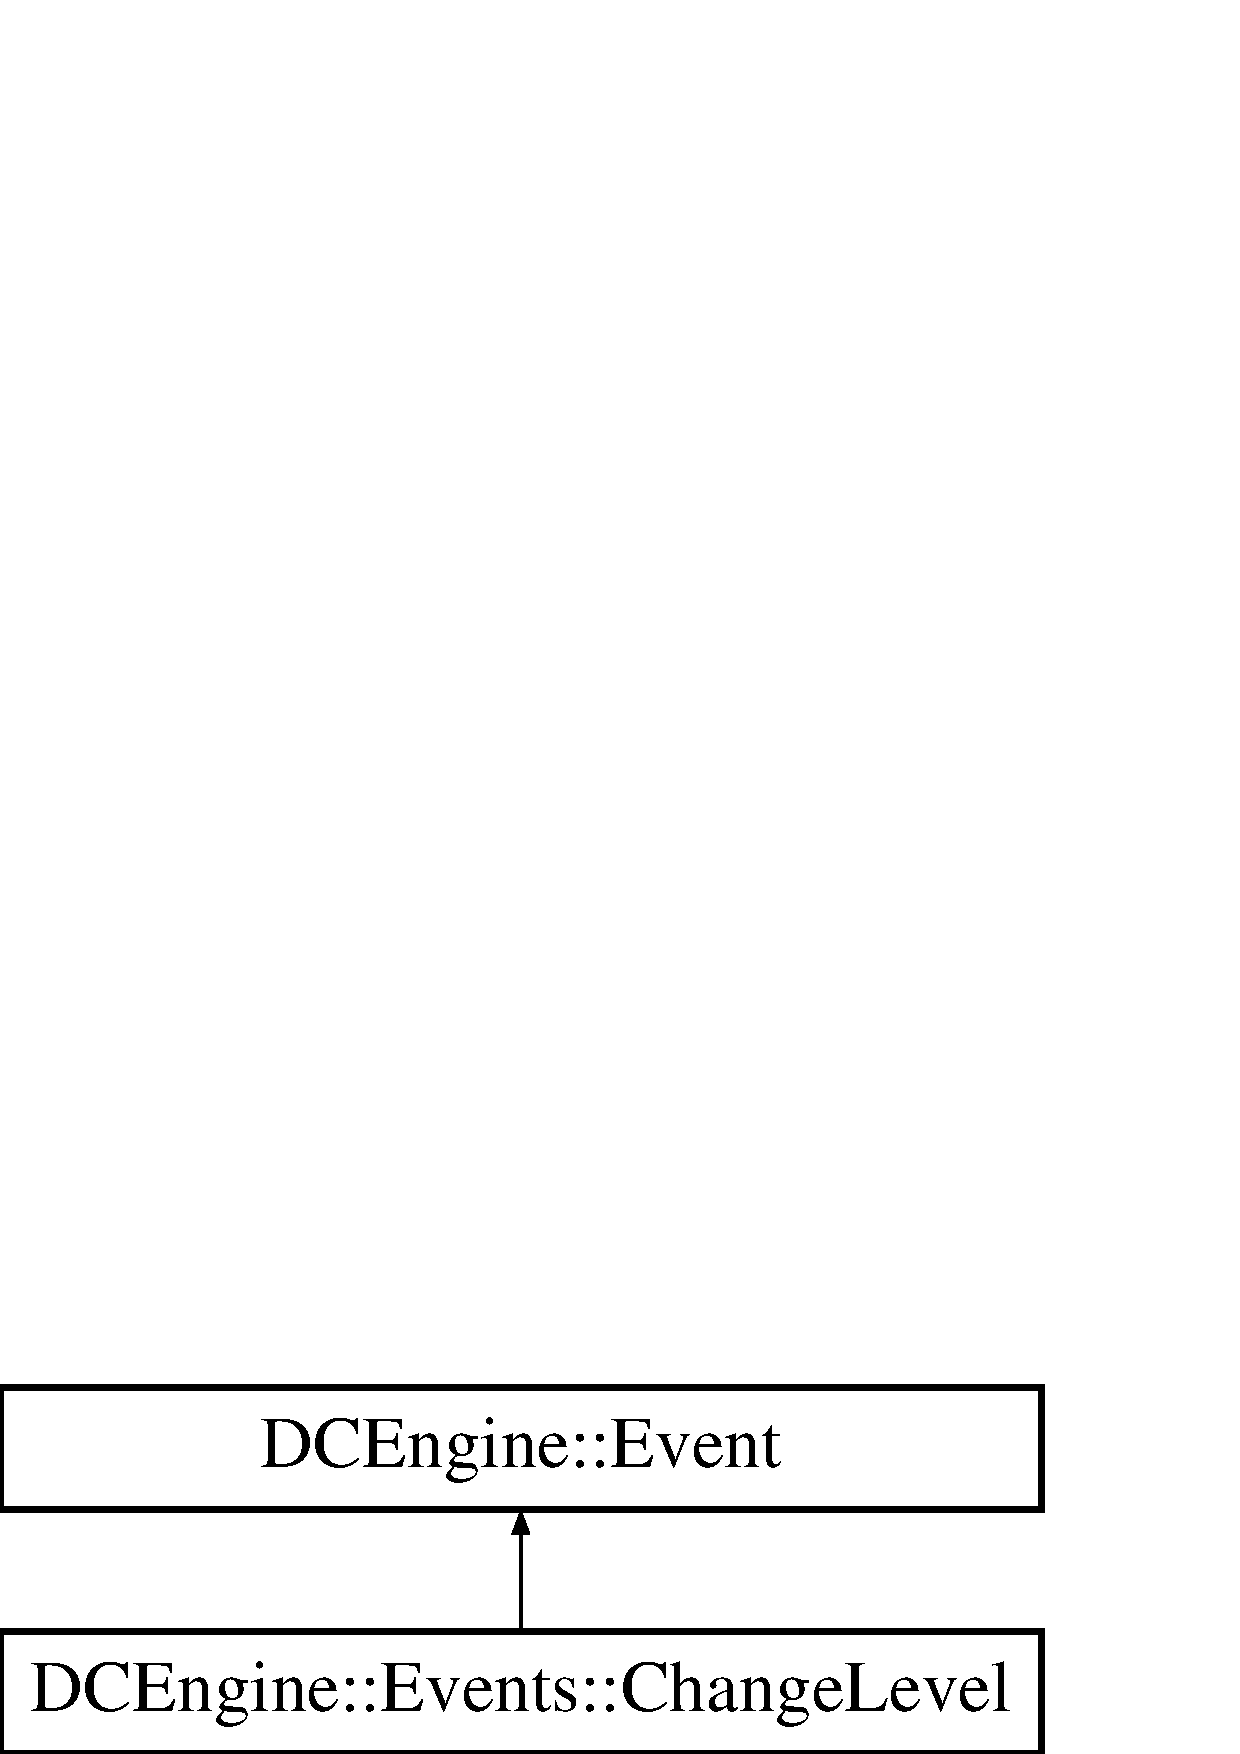
\includegraphics[height=2.000000cm]{classDCEngine_1_1Events_1_1ChangeLevel}
\end{center}
\end{figure}
\subsection*{Public Attributes}
\begin{DoxyCompactItemize}
\item 
\hypertarget{classDCEngine_1_1Events_1_1ChangeLevel_a074a7f37f4b51ecbf97e6c3bfdbdfc0b}{String {\bfseries Next\-Level}}\label{classDCEngine_1_1Events_1_1ChangeLevel_a074a7f37f4b51ecbf97e6c3bfdbdfc0b}

\end{DoxyCompactItemize}
\subsection*{Additional Inherited Members}


The documentation for this class was generated from the following file\-:\begin{DoxyCompactItemize}
\item 
Projects/\-Rebound/\hyperlink{ReboundEvents_8h}{Rebound\-Events.\-h}\end{DoxyCompactItemize}

\hypertarget{classDCEngine_1_1Events_1_1ChangeMusic}{\section{D\-C\-Engine\-:\-:Events\-:\-:Change\-Music Class Reference}
\label{classDCEngine_1_1Events_1_1ChangeMusic}\index{D\-C\-Engine\-::\-Events\-::\-Change\-Music@{D\-C\-Engine\-::\-Events\-::\-Change\-Music}}
}
Inheritance diagram for D\-C\-Engine\-:\-:Events\-:\-:Change\-Music\-:\begin{figure}[H]
\begin{center}
\leavevmode
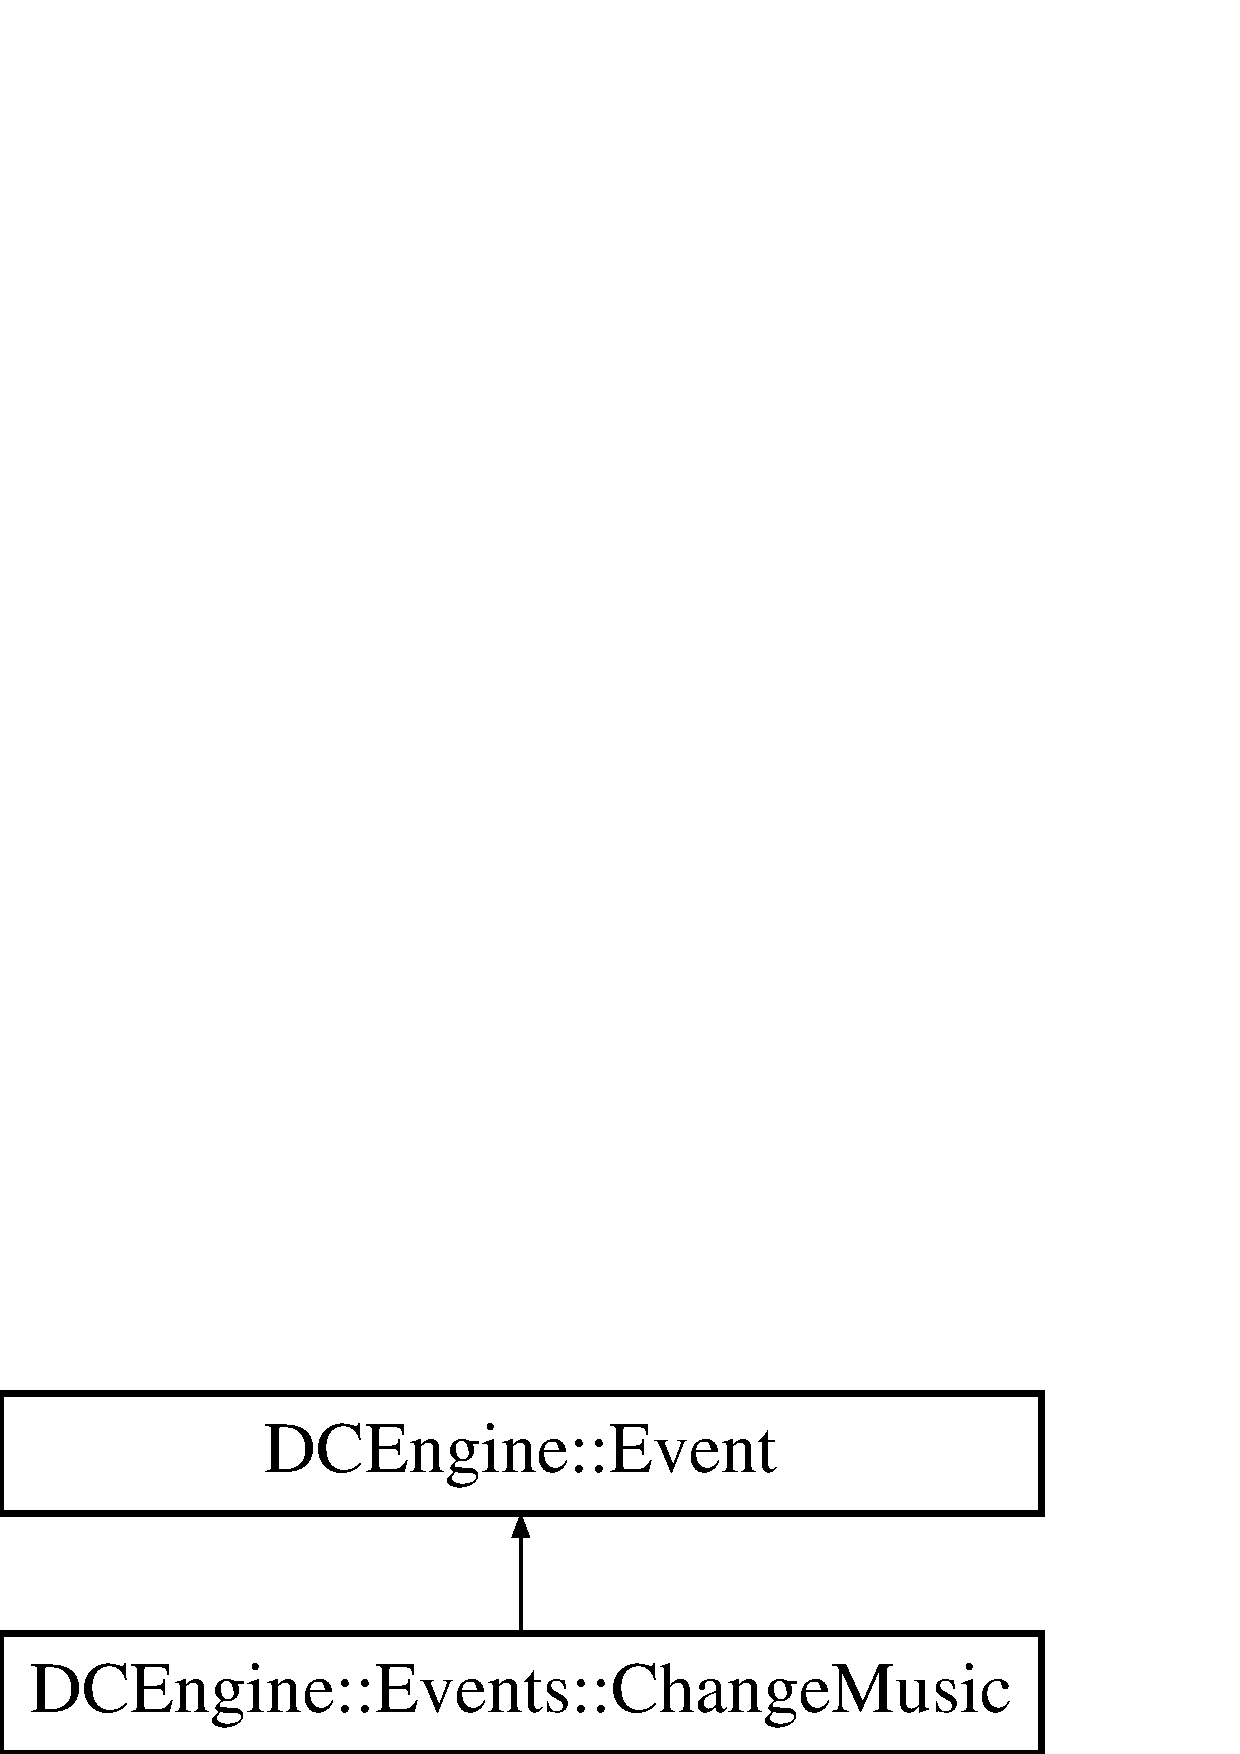
\includegraphics[height=2.000000cm]{classDCEngine_1_1Events_1_1ChangeMusic}
\end{center}
\end{figure}
\subsection*{Public Attributes}
\begin{DoxyCompactItemize}
\item 
\hypertarget{classDCEngine_1_1Events_1_1ChangeMusic_aa76e424e9382ce2713ac02ed9870a64d}{String {\bfseries Next\-Track}}\label{classDCEngine_1_1Events_1_1ChangeMusic_aa76e424e9382ce2713ac02ed9870a64d}

\end{DoxyCompactItemize}
\subsection*{Additional Inherited Members}


The documentation for this class was generated from the following file\-:\begin{DoxyCompactItemize}
\item 
Projects/\-Rebound/\hyperlink{ReboundEvents_8h}{Rebound\-Events.\-h}\end{DoxyCompactItemize}

\hypertarget{structDCEngine_1_1Character}{\section{D\-C\-Engine\-:\-:Character Struct Reference}
\label{structDCEngine_1_1Character}\index{D\-C\-Engine\-::\-Character@{D\-C\-Engine\-::\-Character}}
}


\hyperlink{classA}{A} struct containing generated data about a specific character that will be used whenever it needs to be rendered.  




{\ttfamily \#include $<$Font.\-h$>$}

\subsection*{Public Attributes}
\begin{DoxyCompactItemize}
\item 
\hypertarget{structDCEngine_1_1Character_a6ccc6a669e788621f5ce5c17d2cc91d0}{G\-Luint {\bfseries Character\-Texture\-I\-D}}\label{structDCEngine_1_1Character_a6ccc6a669e788621f5ce5c17d2cc91d0}

\item 
\hypertarget{structDCEngine_1_1Character_a6c3888a28620dce20b10d90f8c2463b1}{glm\-::ivec2 {\bfseries Size}}\label{structDCEngine_1_1Character_a6c3888a28620dce20b10d90f8c2463b1}

\item 
\hypertarget{structDCEngine_1_1Character_aef0f74189925807fe180f1aea85aab7e}{glm\-::ivec2 {\bfseries Bearing}}\label{structDCEngine_1_1Character_aef0f74189925807fe180f1aea85aab7e}

\item 
\hypertarget{structDCEngine_1_1Character_a32bba68b7844b8d18d2a7498fe2a8cc2}{G\-Luint {\bfseries Advance}}\label{structDCEngine_1_1Character_a32bba68b7844b8d18d2a7498fe2a8cc2}

\end{DoxyCompactItemize}


\subsection{Detailed Description}
\hyperlink{classA}{A} struct containing generated data about a specific character that will be used whenever it needs to be rendered. 

The documentation for this struct was generated from the following file\-:\begin{DoxyCompactItemize}
\item 
Core/\-Resources/\hyperlink{Font_8h}{Font.\-h}\end{DoxyCompactItemize}

\hypertarget{structCharacter}{\section{Character Struct Reference}
\label{structCharacter}\index{Character@{Character}}
}


Holds all state information relevant to a character as loaded using Free\-Type.  


\subsection*{Public Attributes}
\begin{DoxyCompactItemize}
\item 
\hypertarget{structCharacter_a51d894cc31d79e95fe1a47fb65c6e889}{G\-Luint {\bfseries Texture\-I\-D}}\label{structCharacter_a51d894cc31d79e95fe1a47fb65c6e889}

\item 
\hypertarget{structCharacter_aaaa598050e0ef590fe6903fd2bab40b8}{glm\-::ivec2 {\bfseries Size}}\label{structCharacter_aaaa598050e0ef590fe6903fd2bab40b8}

\item 
\hypertarget{structCharacter_afef98bf9c7f5313d96476f6f3f85f872}{glm\-::ivec2 {\bfseries Bearing}}\label{structCharacter_afef98bf9c7f5313d96476f6f3f85f872}

\item 
\hypertarget{structCharacter_ab35bae8be6740729fc5839c237a659f6}{G\-Luint {\bfseries Advance}}\label{structCharacter_ab35bae8be6740729fc5839c237a659f6}

\end{DoxyCompactItemize}


\subsection{Detailed Description}
Holds all state information relevant to a character as loaded using Free\-Type. 

The documentation for this struct was generated from the following file\-:\begin{DoxyCompactItemize}
\item 
Projects/Sprite\-Text\-Test.\-cpp\end{DoxyCompactItemize}

\hypertarget{classDCEngine_1_1Components_1_1ChargeBar}{\section{D\-C\-Engine\-:\-:Components\-:\-:Charge\-Bar Class Reference}
\label{classDCEngine_1_1Components_1_1ChargeBar}\index{D\-C\-Engine\-::\-Components\-::\-Charge\-Bar@{D\-C\-Engine\-::\-Components\-::\-Charge\-Bar}}
}
Inheritance diagram for D\-C\-Engine\-:\-:Components\-:\-:Charge\-Bar\-:\begin{figure}[H]
\begin{center}
\leavevmode
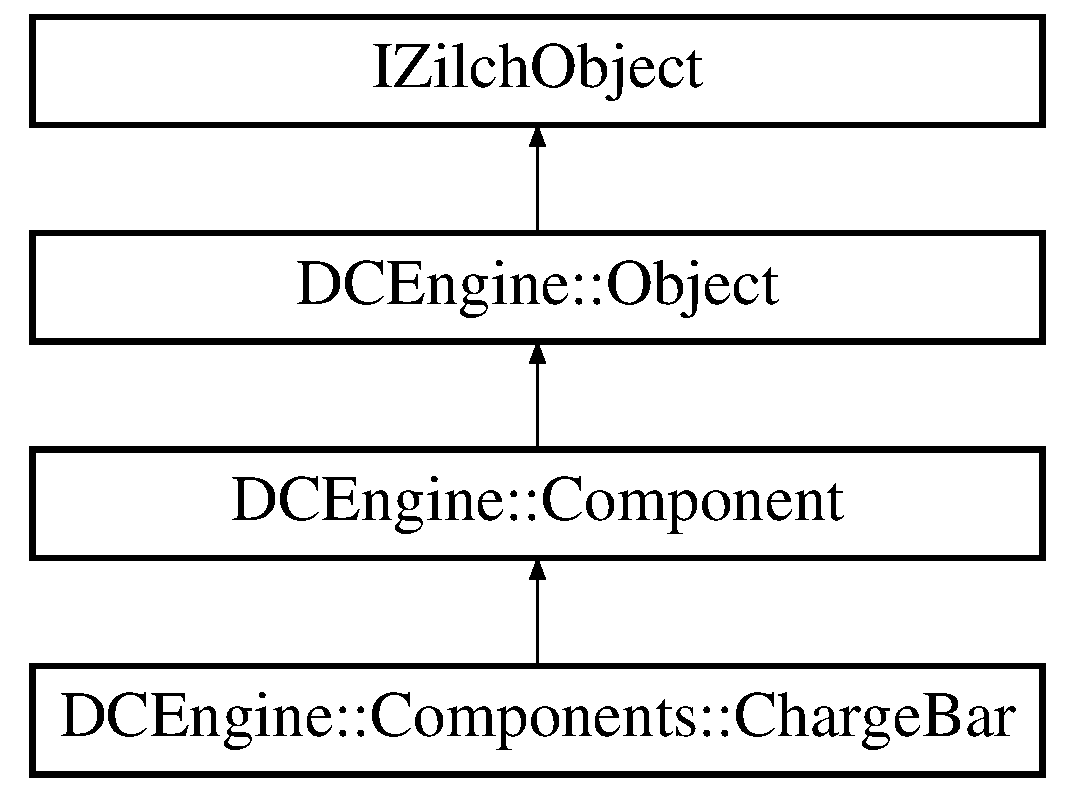
\includegraphics[height=4.000000cm]{classDCEngine_1_1Components_1_1ChargeBar}
\end{center}
\end{figure}
\subsection*{Public Member Functions}
\begin{DoxyCompactItemize}
\item 
\hypertarget{classDCEngine_1_1Components_1_1ChargeBar_a12cf7abcf6848763e8c2a16d8742967a}{{\bfseries D\-C\-E\-\_\-\-D\-E\-F\-I\-N\-E\-\_\-\-P\-R\-O\-P\-E\-R\-T\-Y} (Real, Scale\-X)}\label{classDCEngine_1_1Components_1_1ChargeBar_a12cf7abcf6848763e8c2a16d8742967a}

\item 
\hypertarget{classDCEngine_1_1Components_1_1ChargeBar_a520c05355566455db5f9ee842b0143db}{{\bfseries Charge\-Bar} (\hyperlink{classDCEngine_1_1Entity}{Entity} \&owner)}\label{classDCEngine_1_1Components_1_1ChargeBar_a520c05355566455db5f9ee842b0143db}

\item 
\hypertarget{classDCEngine_1_1Components_1_1ChargeBar_a24241ddbf4aa4584bd81784388608aa5}{void {\bfseries Initialize} ()}\label{classDCEngine_1_1Components_1_1ChargeBar_a24241ddbf4aa4584bd81784388608aa5}

\item 
\hypertarget{classDCEngine_1_1Components_1_1ChargeBar_a882ce7780f27fc039314ae9e8704026d}{virtual void {\bfseries Serialize} (Json\-::\-Value \&root)}\label{classDCEngine_1_1Components_1_1ChargeBar_a882ce7780f27fc039314ae9e8704026d}

\item 
\hypertarget{classDCEngine_1_1Components_1_1ChargeBar_abb0a733a8acaf24a0f95638909614053}{virtual void {\bfseries Deserialize} (Json\-::\-Value \&root)}\label{classDCEngine_1_1Components_1_1ChargeBar_abb0a733a8acaf24a0f95638909614053}

\item 
\hypertarget{classDCEngine_1_1Components_1_1ChargeBar_aa03de6a9e167207f6b97474427fe0d0e}{void {\bfseries On\-Mouse\-Down\-Event} (\hyperlink{classDCEngine_1_1Events_1_1MouseDown}{Events\-::\-Mouse\-Down} $\ast$event)}\label{classDCEngine_1_1Components_1_1ChargeBar_aa03de6a9e167207f6b97474427fe0d0e}

\item 
\hypertarget{classDCEngine_1_1Components_1_1ChargeBar_a09fb506b87d4ace2d3524bee17dd0361}{void {\bfseries On\-Mouse\-Up\-Event} (\hyperlink{classDCEngine_1_1Events_1_1MouseUp}{Events\-::\-Mouse\-Up} $\ast$event)}\label{classDCEngine_1_1Components_1_1ChargeBar_a09fb506b87d4ace2d3524bee17dd0361}

\item 
\hypertarget{classDCEngine_1_1Components_1_1ChargeBar_a3468e17a00bdbb9dd028845fb75dea45}{void {\bfseries Charge\-Bar\-::\-On\-Logic\-Update\-Event} (\hyperlink{classDCEngine_1_1Events_1_1LogicUpdate}{Events\-::\-Logic\-Update} $\ast$event)}\label{classDCEngine_1_1Components_1_1ChargeBar_a3468e17a00bdbb9dd028845fb75dea45}

\item 
\hypertarget{classDCEngine_1_1Components_1_1ChargeBar_a451e089900b0024cc37d6c56d8d595f6}{{\bfseries Zilch\-Declare\-Derived\-Type} (\hyperlink{classDCEngine_1_1Components_1_1ChargeBar}{Charge\-Bar}, \hyperlink{classDCEngine_1_1Component}{Component})}\label{classDCEngine_1_1Components_1_1ChargeBar_a451e089900b0024cc37d6c56d8d595f6}

\end{DoxyCompactItemize}
\subsection*{Public Attributes}
\begin{DoxyCompactItemize}
\item 
\hypertarget{classDCEngine_1_1Components_1_1ChargeBar_a819410826366be6b5c6ae4679fd29420}{\hyperlink{classDCEngine_1_1Components_1_1Transform}{Transform} $\ast$ {\bfseries Transform\-Ref}}\label{classDCEngine_1_1Components_1_1ChargeBar_a819410826366be6b5c6ae4679fd29420}

\item 
\hypertarget{classDCEngine_1_1Components_1_1ChargeBar_af44d439a53a7d34d55154fb97a21f7a7}{\hyperlink{classDCEngine_1_1Components_1_1Sprite}{Sprite} $\ast$ {\bfseries Sprite\-Ref}}\label{classDCEngine_1_1Components_1_1ChargeBar_af44d439a53a7d34d55154fb97a21f7a7}

\item 
\hypertarget{classDCEngine_1_1Components_1_1ChargeBar_a7bdb6793eed0ab0b4d6be43e9e84a60a}{\hyperlink{classDCEngine_1_1GameObject}{Game\-Object} $\ast$ {\bfseries Ball\-Ref}}\label{classDCEngine_1_1Components_1_1ChargeBar_a7bdb6793eed0ab0b4d6be43e9e84a60a}

\item 
\hypertarget{classDCEngine_1_1Components_1_1ChargeBar_aa41a40c70123b6834d99f38abc7ec6c7}{Real {\bfseries Scale\-X} = 2.\-5}\label{classDCEngine_1_1Components_1_1ChargeBar_aa41a40c70123b6834d99f38abc7ec6c7}

\end{DoxyCompactItemize}
\subsection*{Additional Inherited Members}


The documentation for this class was generated from the following files\-:\begin{DoxyCompactItemize}
\item 
Projects/\-Rebound/\-Components/\hyperlink{ChargeBar_8h}{Charge\-Bar.\-h}\item 
Projects/\-Rebound/\-Components/\hyperlink{ChargeBar_8cpp}{Charge\-Bar.\-cpp}\end{DoxyCompactItemize}

\hypertarget{classDCEngine_1_1Components_1_1CircleCollider}{\section{D\-C\-Engine\-:\-:Components\-:\-:Circle\-Collider Class Reference}
\label{classDCEngine_1_1Components_1_1CircleCollider}\index{D\-C\-Engine\-::\-Components\-::\-Circle\-Collider@{D\-C\-Engine\-::\-Components\-::\-Circle\-Collider}}
}
Inheritance diagram for D\-C\-Engine\-:\-:Components\-:\-:Circle\-Collider\-:\begin{figure}[H]
\begin{center}
\leavevmode
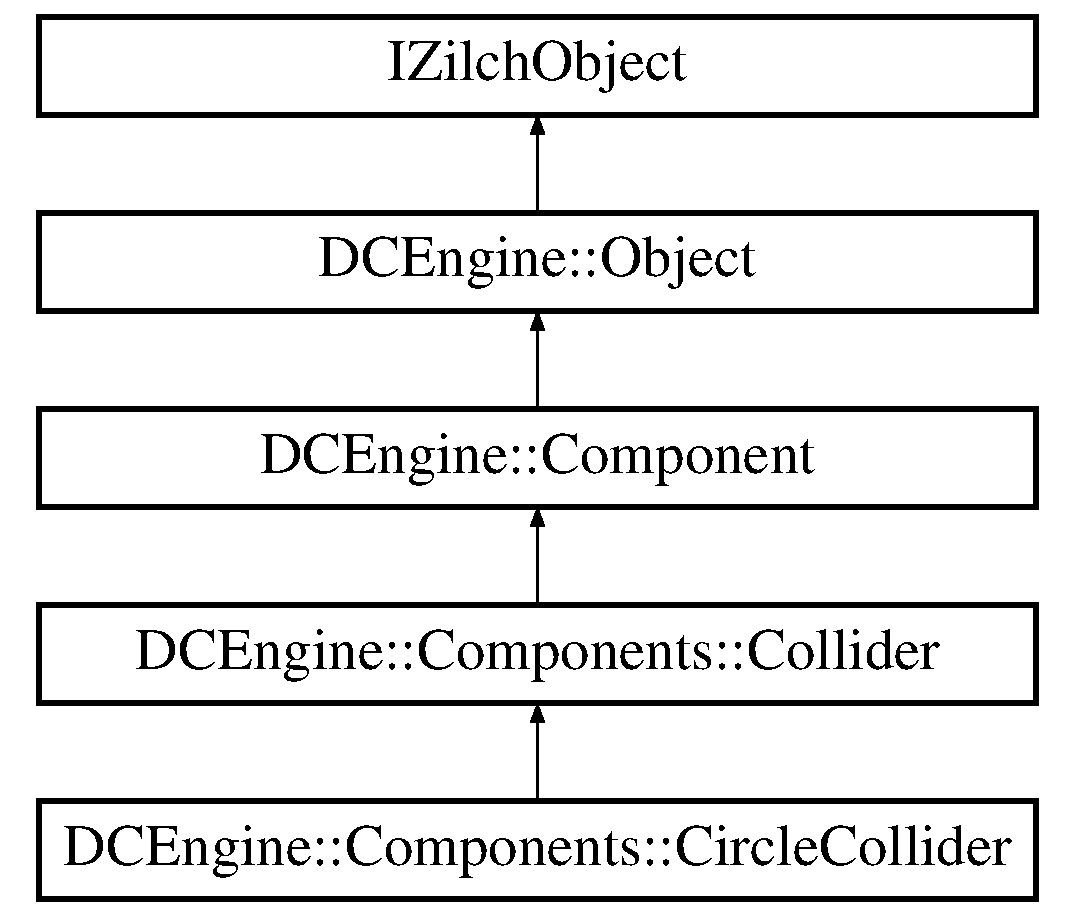
\includegraphics[height=5.000000cm]{classDCEngine_1_1Components_1_1CircleCollider}
\end{center}
\end{figure}
\subsection*{Public Member Functions}
\begin{DoxyCompactItemize}
\item 
\hypertarget{classDCEngine_1_1Components_1_1CircleCollider_a7a2a52f4b5f0d6ec1de8eb4281800395}{float {\bfseries get\-Radius} (void)}\label{classDCEngine_1_1Components_1_1CircleCollider_a7a2a52f4b5f0d6ec1de8eb4281800395}

\item 
\hypertarget{classDCEngine_1_1Components_1_1CircleCollider_a9fff920739e4edeb45022b05689aa53d}{Vec3 {\bfseries get\-Offset} (void)}\label{classDCEngine_1_1Components_1_1CircleCollider_a9fff920739e4edeb45022b05689aa53d}

\item 
\hypertarget{classDCEngine_1_1Components_1_1CircleCollider_afc1e54256ef4a5caaaddaed2719e5deb}{bool {\bfseries get\-Ghost} (void)}\label{classDCEngine_1_1Components_1_1CircleCollider_afc1e54256ef4a5caaaddaed2719e5deb}

\item 
\hypertarget{classDCEngine_1_1Components_1_1CircleCollider_a8398ef07de2906a06513c6fa6ed53cc3}{bool {\bfseries get\-Sends\-Events} (void)}\label{classDCEngine_1_1Components_1_1CircleCollider_a8398ef07de2906a06513c6fa6ed53cc3}

\item 
\hypertarget{classDCEngine_1_1Components_1_1CircleCollider_a5d1d2a2b01967d8aa57c5fd605218efb}{String {\bfseries get\-Collision\-Group} () const }\label{classDCEngine_1_1Components_1_1CircleCollider_a5d1d2a2b01967d8aa57c5fd605218efb}

\item 
\hypertarget{classDCEngine_1_1Components_1_1CircleCollider_ae9b1c031ac7cc98f02d925b0665af12a}{{\bfseries Circle\-Collider} (\hyperlink{classDCEngine_1_1Entity}{Entity} \&owner)}\label{classDCEngine_1_1Components_1_1CircleCollider_ae9b1c031ac7cc98f02d925b0665af12a}

\item 
\hyperlink{classDCEngine_1_1Components_1_1CircleCollider_a531609803e58204df4bd0ae87cbb2a6c}{$\sim$\-Circle\-Collider} ()
\begin{DoxyCompactList}\small\item\em \hyperlink{classDCEngine_1_1Components_1_1CircleCollider}{Circle\-Collider} destructor. \end{DoxyCompactList}\item 
void \hyperlink{classDCEngine_1_1Components_1_1CircleCollider_ae73db7b317b8459a7213270b74254375}{Initialize} ()
\begin{DoxyCompactList}\small\item\em Initializes the \hyperlink{classDCEngine_1_1Components_1_1CircleCollider}{Circle\-Collider} component. \end{DoxyCompactList}\item 
\hypertarget{classDCEngine_1_1Components_1_1CircleCollider_a58c5da0a0a551eadb66404466e8919c2}{void {\bfseries On\-Logic\-Update\-Event} (\hyperlink{classDCEngine_1_1Events_1_1LogicUpdate}{Events\-::\-Logic\-Update} $\ast$event)}\label{classDCEngine_1_1Components_1_1CircleCollider_a58c5da0a0a551eadb66404466e8919c2}

\item 
\hypertarget{classDCEngine_1_1Components_1_1CircleCollider_a5e339d4f1e6707df3aff225ec99408e0}{void \hyperlink{classDCEngine_1_1Components_1_1CircleCollider_a5e339d4f1e6707df3aff225ec99408e0}{On\-Collision\-Started\-Event} (\hyperlink{classDCEngine_1_1Events_1_1CollisionStarted}{Events\-::\-Collision\-Started} $\ast$event)}\label{classDCEngine_1_1Components_1_1CircleCollider_a5e339d4f1e6707df3aff225ec99408e0}

\begin{DoxyCompactList}\small\item\em Collision\-Events. \end{DoxyCompactList}\item 
\hypertarget{classDCEngine_1_1Components_1_1CircleCollider_ab1c1a21c469b4de979514d10c20d9f73}{void {\bfseries On\-Collision\-Ended\-Event} (\hyperlink{classDCEngine_1_1Events_1_1CollisionEnded}{Events\-::\-Collision\-Ended} $\ast$event)}\label{classDCEngine_1_1Components_1_1CircleCollider_ab1c1a21c469b4de979514d10c20d9f73}

\end{DoxyCompactItemize}
\subsection*{Public Attributes}
\begin{DoxyCompactItemize}
\item 
\hypertarget{classDCEngine_1_1Components_1_1CircleCollider_ae82cd959fb0cbdd1f509f37934bc99fa}{float {\bfseries Radius} = 5}\label{classDCEngine_1_1Components_1_1CircleCollider_ae82cd959fb0cbdd1f509f37934bc99fa}

\item 
\hypertarget{classDCEngine_1_1Components_1_1CircleCollider_a8b32bdab767a6fb69a7ce4773121298b}{Vec3 {\bfseries Offset} = Vec3(0, 0, 0)}\label{classDCEngine_1_1Components_1_1CircleCollider_a8b32bdab767a6fb69a7ce4773121298b}

\item 
\hypertarget{classDCEngine_1_1Components_1_1CircleCollider_aa4d656f4fa5d4d884f86e56a427eccd7}{Boolean {\bfseries Ghost} = false}\label{classDCEngine_1_1Components_1_1CircleCollider_aa4d656f4fa5d4d884f86e56a427eccd7}

\item 
\hypertarget{classDCEngine_1_1Components_1_1CircleCollider_a380e5b9f11b65797209d17dcb36a9d4e}{Boolean {\bfseries Sends\-Events} = true}\label{classDCEngine_1_1Components_1_1CircleCollider_a380e5b9f11b65797209d17dcb36a9d4e}

\item 
\hypertarget{classDCEngine_1_1Components_1_1CircleCollider_ad452538f05e38f7f927a312681467d30}{Boolean {\bfseries Is\-Drawing\-Collider} = false}\label{classDCEngine_1_1Components_1_1CircleCollider_ad452538f05e38f7f927a312681467d30}

\end{DoxyCompactItemize}
\subsection*{Additional Inherited Members}


\subsection{Constructor \& Destructor Documentation}
\hypertarget{classDCEngine_1_1Components_1_1CircleCollider_a531609803e58204df4bd0ae87cbb2a6c}{\index{D\-C\-Engine\-::\-Components\-::\-Circle\-Collider@{D\-C\-Engine\-::\-Components\-::\-Circle\-Collider}!$\sim$\-Circle\-Collider@{$\sim$\-Circle\-Collider}}
\index{$\sim$\-Circle\-Collider@{$\sim$\-Circle\-Collider}!DCEngine::Components::CircleCollider@{D\-C\-Engine\-::\-Components\-::\-Circle\-Collider}}
\subsubsection[{$\sim$\-Circle\-Collider}]{\setlength{\rightskip}{0pt plus 5cm}D\-C\-Engine\-::\-Components\-::\-Circle\-Collider\-::$\sim$\-Circle\-Collider (
\begin{DoxyParamCaption}
{}
\end{DoxyParamCaption}
)}}\label{classDCEngine_1_1Components_1_1CircleCollider_a531609803e58204df4bd0ae87cbb2a6c}


\hyperlink{classDCEngine_1_1Components_1_1CircleCollider}{Circle\-Collider} destructor. 

\begin{DoxyRefDesc}{Todo}
\item[\hyperlink{todo__todo000001}{Todo}]This could be done in the base collider class instead. \end{DoxyRefDesc}


\subsection{Member Function Documentation}
\hypertarget{classDCEngine_1_1Components_1_1CircleCollider_ae73db7b317b8459a7213270b74254375}{\index{D\-C\-Engine\-::\-Components\-::\-Circle\-Collider@{D\-C\-Engine\-::\-Components\-::\-Circle\-Collider}!Initialize@{Initialize}}
\index{Initialize@{Initialize}!DCEngine::Components::CircleCollider@{D\-C\-Engine\-::\-Components\-::\-Circle\-Collider}}
\subsubsection[{Initialize}]{\setlength{\rightskip}{0pt plus 5cm}void D\-C\-Engine\-::\-Components\-::\-Circle\-Collider\-::\-Initialize (
\begin{DoxyParamCaption}
{}
\end{DoxyParamCaption}
)\hspace{0.3cm}{\ttfamily [virtual]}}}\label{classDCEngine_1_1Components_1_1CircleCollider_ae73db7b317b8459a7213270b74254375}


Initializes the \hyperlink{classDCEngine_1_1Components_1_1CircleCollider}{Circle\-Collider} component. 

\begin{DoxyNote}{Note}
This can only go in the translational unit (.cpp) 
\end{DoxyNote}


Reimplemented from \hyperlink{classDCEngine_1_1Components_1_1Collider_a805e62e849eaad2bdfd12f9f904bc698}{D\-C\-Engine\-::\-Components\-::\-Collider}.



The documentation for this class was generated from the following files\-:\begin{DoxyCompactItemize}
\item 
Core/\-Components/\hyperlink{CircleCollider_8h}{Circle\-Collider.\-h}\item 
Core/\-Components/\hyperlink{CircleCollider_8cpp}{Circle\-Collider.\-cpp}\end{DoxyCompactItemize}

\hypertarget{classDCEngine_1_1Components_1_1Collider}{\section{D\-C\-Engine\-:\-:Components\-:\-:Collider Class Reference}
\label{classDCEngine_1_1Components_1_1Collider}\index{D\-C\-Engine\-::\-Components\-::\-Collider@{D\-C\-Engine\-::\-Components\-::\-Collider}}
}
Inheritance diagram for D\-C\-Engine\-:\-:Components\-:\-:Collider\-:\begin{figure}[H]
\begin{center}
\leavevmode
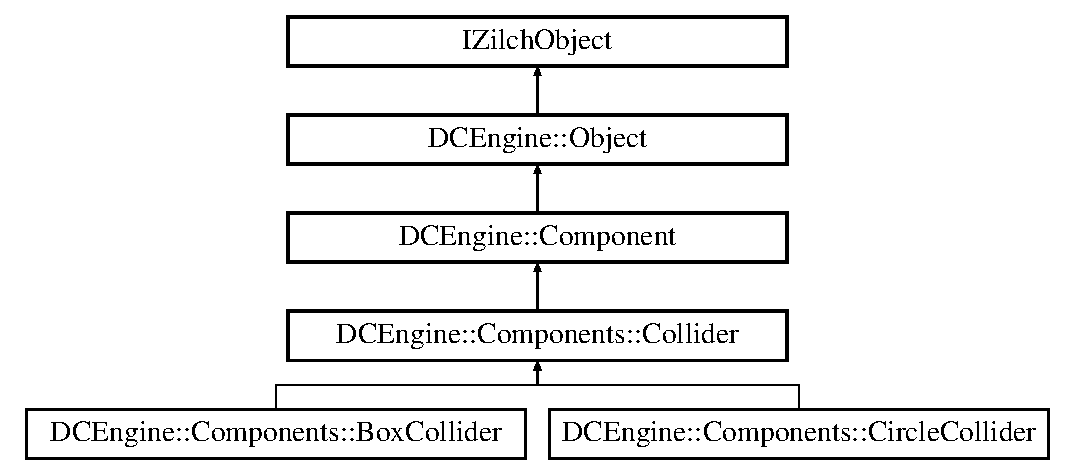
\includegraphics[height=5.000000cm]{classDCEngine_1_1Components_1_1Collider}
\end{center}
\end{figure}
\subsection*{Public Member Functions}
\begin{DoxyCompactItemize}
\item 
\hypertarget{classDCEngine_1_1Components_1_1Collider_a2ce1675659faea8ea65e29e4d4bcf1a2}{{\bfseries Zilch\-Declare\-Derived\-Type} (\hyperlink{classDCEngine_1_1Components_1_1Collider}{Collider}, \hyperlink{classDCEngine_1_1Component}{Component})}\label{classDCEngine_1_1Components_1_1Collider_a2ce1675659faea8ea65e29e4d4bcf1a2}

\item 
\hypertarget{classDCEngine_1_1Components_1_1Collider_a648f281956bc2ef3db763b98f2a612e8}{{\bfseries D\-C\-E\-\_\-\-D\-E\-F\-I\-N\-E\-\_\-\-P\-R\-O\-P\-E\-R\-T\-Y} (String, \hyperlink{classDCEngine_1_1CollisionGroup}{Collision\-Group})}\label{classDCEngine_1_1Components_1_1Collider_a648f281956bc2ef3db763b98f2a612e8}

\item 
\hyperlink{classDCEngine_1_1Components_1_1Collider_a23fd446735e579c844a9431c57072823}{Collider} (\hyperlink{classDCEngine_1_1Entity}{Entity} \&owner, std\-::string collider\-Class)
\begin{DoxyCompactList}\small\item\em \hyperlink{classDCEngine_1_1Components_1_1Collider}{Collider} constructor. \end{DoxyCompactList}\item 
\hypertarget{classDCEngine_1_1Components_1_1Collider_a1c492143023f9b2552eb662028be9df0}{\hyperlink{classDCEngine_1_1Components_1_1Collider_a1c492143023f9b2552eb662028be9df0}{$\sim$\-Collider} ()}\label{classDCEngine_1_1Components_1_1Collider_a1c492143023f9b2552eb662028be9df0}

\begin{DoxyCompactList}\small\item\em \hyperlink{classDCEngine_1_1Components_1_1Collider}{Collider} destructor. \end{DoxyCompactList}\item 
\hypertarget{classDCEngine_1_1Components_1_1Collider_a805e62e849eaad2bdfd12f9f904bc698}{virtual void \hyperlink{classDCEngine_1_1Components_1_1Collider_a805e62e849eaad2bdfd12f9f904bc698}{Initialize} ()}\label{classDCEngine_1_1Components_1_1Collider_a805e62e849eaad2bdfd12f9f904bc698}

\begin{DoxyCompactList}\small\item\em \hyperlink{classDCEngine_1_1Components_1_1Collider}{Collider} initializer. \end{DoxyCompactList}\end{DoxyCompactItemize}
\subsection*{Static Public Attributes}
\begin{DoxyCompactItemize}
\item 
\hypertarget{classDCEngine_1_1Components_1_1Collider_aa324ce817a0a5ba7457054b56a2834b8}{static unsigned {\bfseries Created} = 0}\label{classDCEngine_1_1Components_1_1Collider_aa324ce817a0a5ba7457054b56a2834b8}

\item 
\hypertarget{classDCEngine_1_1Components_1_1Collider_a61e2b7e248a5855adb85433dd134fdf2}{static unsigned {\bfseries Destroyed} = 0}\label{classDCEngine_1_1Components_1_1Collider_a61e2b7e248a5855adb85433dd134fdf2}

\item 
\hypertarget{classDCEngine_1_1Components_1_1Collider_a6b75d7d21ccb7aed04b4fe97d7ddb932}{static unsigned {\bfseries Active} = 0}\label{classDCEngine_1_1Components_1_1Collider_a6b75d7d21ccb7aed04b4fe97d7ddb932}

\end{DoxyCompactItemize}
\subsection*{Friends}
\begin{DoxyCompactItemize}
\item 
\hypertarget{classDCEngine_1_1Components_1_1Collider_a2bfcbae6c8e1d7af93c5ac1200b1535c}{class {\bfseries Physics}}\label{classDCEngine_1_1Components_1_1Collider_a2bfcbae6c8e1d7af93c5ac1200b1535c}

\end{DoxyCompactItemize}
\subsection*{Additional Inherited Members}


\subsection{Constructor \& Destructor Documentation}
\hypertarget{classDCEngine_1_1Components_1_1Collider_a23fd446735e579c844a9431c57072823}{\index{D\-C\-Engine\-::\-Components\-::\-Collider@{D\-C\-Engine\-::\-Components\-::\-Collider}!Collider@{Collider}}
\index{Collider@{Collider}!DCEngine::Components::Collider@{D\-C\-Engine\-::\-Components\-::\-Collider}}
\subsubsection[{Collider}]{\setlength{\rightskip}{0pt plus 5cm}D\-C\-Engine\-::\-Components\-::\-Collider\-::\-Collider (
\begin{DoxyParamCaption}
\item[{{\bf Entity} \&}]{owner, }
\item[{std\-::string}]{collider\-Class}
\end{DoxyParamCaption}
)}}\label{classDCEngine_1_1Components_1_1Collider_a23fd446735e579c844a9431c57072823}


\hyperlink{classDCEngine_1_1Components_1_1Collider}{Collider} constructor. 


\begin{DoxyParams}{Parameters}
{\em owner} & A reference to the \hyperlink{classDCEngine_1_1Entity}{Entity} that owns this component. \\
\hline
{\em graphical\-Component} & \hyperlink{classThe}{The} name of the derived collider component. \\
\hline
\end{DoxyParams}


The documentation for this class was generated from the following files\-:\begin{DoxyCompactItemize}
\item 
Core/\-Components/\hyperlink{Collider_8h}{Collider.\-h}\item 
Core/\-Components/\hyperlink{Collider_8cpp}{Collider.\-cpp}\end{DoxyCompactItemize}

\hypertarget{classDCEngine_1_1Collision}{\section{D\-C\-Engine\-:\-:Collision Class Reference}
\label{classDCEngine_1_1Collision}\index{D\-C\-Engine\-::\-Collision@{D\-C\-Engine\-::\-Collision}}
}
\subsection*{Static Public Member Functions}
\begin{DoxyCompactItemize}
\item 
static bool \hyperlink{classDCEngine_1_1Collision_a2e374e9c140f0fd3e48a08c7f692ba57}{Boxto\-Box} (\hyperlink{classDCEngine_1_1GameObject}{Game\-Object} $\ast$obj1, \hyperlink{classDCEngine_1_1GameObject}{Game\-Object} $\ast$obj2, \hyperlink{classDCEngine_1_1Manifold}{Manifold} \&result)
\begin{DoxyCompactList}\small\item\em This function determines if two 'Game\-Objects' with the 'Box\-Collider' component are colliding. \end{DoxyCompactList}\item 
static bool \hyperlink{classDCEngine_1_1Collision_a9fe2558f3a401204c2dfd5379314d4a2}{Circleto\-Box} (\hyperlink{classDCEngine_1_1GameObject}{Game\-Object} $\ast$objrect, \hyperlink{classDCEngine_1_1GameObject}{Game\-Object} $\ast$objcircle, \hyperlink{classDCEngine_1_1Manifold}{Manifold} \&result)
\begin{DoxyCompactList}\small\item\em This function determines if two 'Game\-Objects', one with a 'Box\-Collider' component and the other with a 'Sphere\-Collider' component are colliding. \end{DoxyCompactList}\item 
static std\-::vector\\*
$<$ std\-::vector$<$ float $>$ $>$ \hyperlink{classDCEngine_1_1Collision_ae9e4320d7b1593a637fdbe165d6ab60f}{Project\-On\-To} (std\-::vector$<$ glm\-::vec3 $>$ \&verts1, std\-::vector$<$ glm\-::vec3 $>$ \&verts2, glm\-::vec3 \&Axis)
\begin{DoxyCompactList}\small\item\em This function projects an objects verts on to a vector. \end{DoxyCompactList}\item 
static bool \hyperlink{classDCEngine_1_1Collision_a45759dcb29a1d71b00aa5554809bb681}{Circleto\-Circle} (\hyperlink{classDCEngine_1_1GameObject}{Game\-Object} $\ast$obj1, \hyperlink{classDCEngine_1_1GameObject}{Game\-Object} $\ast$obj2, \hyperlink{classDCEngine_1_1Manifold}{Manifold} \&result)
\begin{DoxyCompactList}\small\item\em This function determines if two 'Game\-Objects' with the 'Sphere\-Collider' component are colliding. \end{DoxyCompactList}\item 
\hypertarget{classDCEngine_1_1Collision_aecbf391f9fbb54baeefc67e1bc45a4a4}{static bool {\bfseries Point\-To\-Circle} (\hyperlink{classDCEngine_1_1GameObject}{Game\-Object} $\ast$circle, glm\-::vec3 point)}\label{classDCEngine_1_1Collision_aecbf391f9fbb54baeefc67e1bc45a4a4}

\item 
static bool \hyperlink{classDCEngine_1_1Collision_a576bb4eb8f34b8b7c9e48de0444fee19}{Point\-To\-Rectangle} (\hyperlink{classDCEngine_1_1GameObject}{Game\-Object} $\ast$rect, glm\-::vec3 point)
\begin{DoxyCompactList}\small\item\em Provides the definition of this class to Zilch. \end{DoxyCompactList}\item 
\hypertarget{classDCEngine_1_1Collision_a7dbe241ccaa5fe4891dbfbb8079e1ce9}{static bool {\bfseries Selectionto\-Box} (Vec3 \&center, float width, float height, Vec3 \&translation, Vec3 \&scale, float rot)}\label{classDCEngine_1_1Collision_a7dbe241ccaa5fe4891dbfbb8079e1ce9}

\end{DoxyCompactItemize}


\subsection{Member Function Documentation}
\hypertarget{classDCEngine_1_1Collision_a2e374e9c140f0fd3e48a08c7f692ba57}{\index{D\-C\-Engine\-::\-Collision@{D\-C\-Engine\-::\-Collision}!Boxto\-Box@{Boxto\-Box}}
\index{Boxto\-Box@{Boxto\-Box}!DCEngine::Collision@{D\-C\-Engine\-::\-Collision}}
\subsubsection[{Boxto\-Box}]{\setlength{\rightskip}{0pt plus 5cm}bool D\-C\-Engine\-::\-Collision\-::\-Boxto\-Box (
\begin{DoxyParamCaption}
\item[{{\bf Game\-Object} $\ast$}]{obj1, }
\item[{{\bf Game\-Object} $\ast$}]{obj2, }
\item[{{\bf Manifold} \&}]{result}
\end{DoxyParamCaption}
)\hspace{0.3cm}{\ttfamily [static]}}}\label{classDCEngine_1_1Collision_a2e374e9c140f0fd3e48a08c7f692ba57}


This function determines if two 'Game\-Objects' with the 'Box\-Collider' component are colliding. 


\begin{DoxyParams}{Parameters}
{\em A} & pointer to the first object. \\
\hline
{\em A} & pointer to the second object. \\
\hline
\end{DoxyParams}
\begin{DoxyReturn}{Returns}
True if a collision was detected, false otherwise. 
\end{DoxyReturn}
\hypertarget{classDCEngine_1_1Collision_a9fe2558f3a401204c2dfd5379314d4a2}{\index{D\-C\-Engine\-::\-Collision@{D\-C\-Engine\-::\-Collision}!Circleto\-Box@{Circleto\-Box}}
\index{Circleto\-Box@{Circleto\-Box}!DCEngine::Collision@{D\-C\-Engine\-::\-Collision}}
\subsubsection[{Circleto\-Box}]{\setlength{\rightskip}{0pt plus 5cm}bool D\-C\-Engine\-::\-Collision\-::\-Circleto\-Box (
\begin{DoxyParamCaption}
\item[{{\bf Game\-Object} $\ast$}]{objrect, }
\item[{{\bf Game\-Object} $\ast$}]{objcircle, }
\item[{{\bf Manifold} \&}]{result}
\end{DoxyParamCaption}
)\hspace{0.3cm}{\ttfamily [static]}}}\label{classDCEngine_1_1Collision_a9fe2558f3a401204c2dfd5379314d4a2}


This function determines if two 'Game\-Objects', one with a 'Box\-Collider' component and the other with a 'Sphere\-Collider' component are colliding. 


\begin{DoxyParams}{Parameters}
{\em A} & pointer to the first object with the 'Box\-Collider'. \\
\hline
{\em A} & pointer to the second object with the 'Sphere\-Collider'. \\
\hline
\end{DoxyParams}
\begin{DoxyReturn}{Returns}
True if a collision was detected, false otherwise. 
\end{DoxyReturn}
\hypertarget{classDCEngine_1_1Collision_a45759dcb29a1d71b00aa5554809bb681}{\index{D\-C\-Engine\-::\-Collision@{D\-C\-Engine\-::\-Collision}!Circleto\-Circle@{Circleto\-Circle}}
\index{Circleto\-Circle@{Circleto\-Circle}!DCEngine::Collision@{D\-C\-Engine\-::\-Collision}}
\subsubsection[{Circleto\-Circle}]{\setlength{\rightskip}{0pt plus 5cm}bool D\-C\-Engine\-::\-Collision\-::\-Circleto\-Circle (
\begin{DoxyParamCaption}
\item[{{\bf Game\-Object} $\ast$}]{obj1, }
\item[{{\bf Game\-Object} $\ast$}]{obj2, }
\item[{{\bf Manifold} \&}]{result}
\end{DoxyParamCaption}
)\hspace{0.3cm}{\ttfamily [static]}}}\label{classDCEngine_1_1Collision_a45759dcb29a1d71b00aa5554809bb681}


This function determines if two 'Game\-Objects' with the 'Sphere\-Collider' component are colliding. 


\begin{DoxyParams}{Parameters}
{\em A} & pointer to the first object. \\
\hline
{\em A} & pointer to the second object. \\
\hline
\end{DoxyParams}
\begin{DoxyReturn}{Returns}
True if a collision was detected, false otherwise. 
\end{DoxyReturn}
\hypertarget{classDCEngine_1_1Collision_a576bb4eb8f34b8b7c9e48de0444fee19}{\index{D\-C\-Engine\-::\-Collision@{D\-C\-Engine\-::\-Collision}!Point\-To\-Rectangle@{Point\-To\-Rectangle}}
\index{Point\-To\-Rectangle@{Point\-To\-Rectangle}!DCEngine::Collision@{D\-C\-Engine\-::\-Collision}}
\subsubsection[{Point\-To\-Rectangle}]{\setlength{\rightskip}{0pt plus 5cm}bool D\-C\-Engine\-::\-Collision\-::\-Point\-To\-Rectangle (
\begin{DoxyParamCaption}
\item[{{\bf Game\-Object} $\ast$}]{rect, }
\item[{glm\-::vec3}]{point}
\end{DoxyParamCaption}
)\hspace{0.3cm}{\ttfamily [static]}}}\label{classDCEngine_1_1Collision_a576bb4eb8f34b8b7c9e48de0444fee19}


Provides the definition of this class to Zilch. 


\begin{DoxyParams}{Parameters}
{\em @param} & \\
\hline
\end{DoxyParams}
\begin{DoxyReturn}{Returns}

\end{DoxyReturn}
\begin{DoxyRefDesc}{Todo}
\item[\hyperlink{todo__todo000049}{Todo}]Look at the comment. \end{DoxyRefDesc}
\hypertarget{classDCEngine_1_1Collision_ae9e4320d7b1593a637fdbe165d6ab60f}{\index{D\-C\-Engine\-::\-Collision@{D\-C\-Engine\-::\-Collision}!Project\-On\-To@{Project\-On\-To}}
\index{Project\-On\-To@{Project\-On\-To}!DCEngine::Collision@{D\-C\-Engine\-::\-Collision}}
\subsubsection[{Project\-On\-To}]{\setlength{\rightskip}{0pt plus 5cm}std\-::vector$<$ std\-::vector$<$ float $>$ $>$ D\-C\-Engine\-::\-Collision\-::\-Project\-On\-To (
\begin{DoxyParamCaption}
\item[{std\-::vector$<$ glm\-::vec3 $>$ \&}]{verts1, }
\item[{std\-::vector$<$ glm\-::vec3 $>$ \&}]{verts2, }
\item[{glm\-::vec3 \&}]{Axis}
\end{DoxyParamCaption}
)\hspace{0.3cm}{\ttfamily [static]}}}\label{classDCEngine_1_1Collision_ae9e4320d7b1593a637fdbe165d6ab60f}


This function projects an objects verts on to a vector. 


\begin{DoxyParams}{Parameters}
{\em vec-\/} & the vector we are projecting. \\
\hline
{\em Axis-\/} & the axis we are projecting on to. \\
\hline
{\em result-\/} & where to store the result. \\
\hline
\end{DoxyParams}


The documentation for this class was generated from the following files\-:\begin{DoxyCompactItemize}
\item 
Core/\-Systems/\-Physics/\hyperlink{Collision_8h}{Collision.\-h}\item 
Core/\-Systems/\-Physics/\hyperlink{Collision_8cpp}{Collision.\-cpp}\end{DoxyCompactItemize}

\hypertarget{structDCEngine_1_1CollisionBlock}{\section{D\-C\-Engine\-:\-:Collision\-Block Struct Reference}
\label{structDCEngine_1_1CollisionBlock}\index{D\-C\-Engine\-::\-Collision\-Block@{D\-C\-Engine\-::\-Collision\-Block}}
}
\subsection*{Public Attributes}
\begin{DoxyCompactItemize}
\item 
bool \hyperlink{structDCEngine_1_1CollisionBlock_a51e7188179af1d8acc25e7c42e887704}{Send\-Events\-To\-A} = true
\begin{DoxyCompactList}\small\item\em $<$ Whether or not to send events to the object of Type\-A in a collision \end{DoxyCompactList}\item 
\hypertarget{structDCEngine_1_1CollisionBlock_a9364f34b3f69a115385ba4216f7293f3}{bool \hyperlink{structDCEngine_1_1CollisionBlock_a9364f34b3f69a115385ba4216f7293f3}{Send\-Events\-To\-B} = true}\label{structDCEngine_1_1CollisionBlock_a9364f34b3f69a115385ba4216f7293f3}

\begin{DoxyCompactList}\small\item\em Wheter or not to send events to the space in a collision of Type\-A and. \end{DoxyCompactList}\item 
\hypertarget{structDCEngine_1_1CollisionBlock_a40abc33b90d9045d76ce6c6de9c21c25}{bool \hyperlink{structDCEngine_1_1CollisionBlock_a40abc33b90d9045d76ce6c6de9c21c25}{Send\-Events\-To\-Space} = true}\label{structDCEngine_1_1CollisionBlock_a40abc33b90d9045d76ce6c6de9c21c25}

\begin{DoxyCompactList}\small\item\em What event name to send out. If left empty the event name will be. \end{DoxyCompactList}\end{DoxyCompactItemize}


\subsection{Member Data Documentation}
\hypertarget{structDCEngine_1_1CollisionBlock_a51e7188179af1d8acc25e7c42e887704}{\index{D\-C\-Engine\-::\-Collision\-Block@{D\-C\-Engine\-::\-Collision\-Block}!Send\-Events\-To\-A@{Send\-Events\-To\-A}}
\index{Send\-Events\-To\-A@{Send\-Events\-To\-A}!DCEngine::CollisionBlock@{D\-C\-Engine\-::\-Collision\-Block}}
\subsubsection[{Send\-Events\-To\-A}]{\setlength{\rightskip}{0pt plus 5cm}bool D\-C\-Engine\-::\-Collision\-Block\-::\-Send\-Events\-To\-A = true}}\label{structDCEngine_1_1CollisionBlock_a51e7188179af1d8acc25e7c42e887704}


$<$ Whether or not to send events to the object of Type\-A in a collision 

Whether or not to send events to the object of Type\-B in a collision 

The documentation for this struct was generated from the following file\-:\begin{DoxyCompactItemize}
\item 
Core/\-Resources/\hyperlink{CollisionTable_8h}{Collision\-Table.\-h}\end{DoxyCompactItemize}

\hypertarget{structDCEngine_1_1CollisionData}{\section{D\-C\-Engine\-:\-:Collision\-Data Struct Reference}
\label{structDCEngine_1_1CollisionData}\index{D\-C\-Engine\-::\-Collision\-Data@{D\-C\-Engine\-::\-Collision\-Data}}
}
\subsection*{Public Attributes}
\begin{DoxyCompactItemize}
\item 
\hypertarget{structDCEngine_1_1CollisionData_a4c363e91902e439d3973349fc9f9956d}{\hyperlink{classDCEngine_1_1GameObject}{Game\-Object} $\ast$ \hyperlink{structDCEngine_1_1CollisionData_a4c363e91902e439d3973349fc9f9956d}{Object}}\label{structDCEngine_1_1CollisionData_a4c363e91902e439d3973349fc9f9956d}

\begin{DoxyCompactList}\small\item\em \hyperlink{classThe}{The} object this event was sent to. \end{DoxyCompactList}\item 
\hypertarget{structDCEngine_1_1CollisionData_a34516d1aa75eebbc7600705b7eef7ab1}{\hyperlink{classDCEngine_1_1GameObject}{Game\-Object} $\ast$ \hyperlink{structDCEngine_1_1CollisionData_a34516d1aa75eebbc7600705b7eef7ab1}{Other\-Object}}\label{structDCEngine_1_1CollisionData_a34516d1aa75eebbc7600705b7eef7ab1}

\begin{DoxyCompactList}\small\item\em \hyperlink{classThe}{The} other object in the collision. \end{DoxyCompactList}\item 
\hypertarget{structDCEngine_1_1CollisionData_a86252b2c37bba3acd2f649a9d0e88762}{\hyperlink{structDCEngine_1_1CollisionFilter}{Collision\-Filter} \hyperlink{structDCEngine_1_1CollisionData_a86252b2c37bba3acd2f649a9d0e88762}{filter}}\label{structDCEngine_1_1CollisionData_a86252b2c37bba3acd2f649a9d0e88762}

\begin{DoxyCompactList}\small\item\em info on what events to send \end{DoxyCompactList}\end{DoxyCompactItemize}


The documentation for this struct was generated from the following file\-:\begin{DoxyCompactItemize}
\item 
Core/\-Systems/\-Physics/\hyperlink{Physics_8h}{Physics.\-h}\end{DoxyCompactItemize}

\hypertarget{classDCEngine_1_1Events_1_1CollisionEnded}{\section{D\-C\-Engine\-:\-:Events\-:\-:Collision\-Ended Class Reference}
\label{classDCEngine_1_1Events_1_1CollisionEnded}\index{D\-C\-Engine\-::\-Events\-::\-Collision\-Ended@{D\-C\-Engine\-::\-Events\-::\-Collision\-Ended}}
}
Inheritance diagram for D\-C\-Engine\-:\-:Events\-:\-:Collision\-Ended\-:\begin{figure}[H]
\begin{center}
\leavevmode
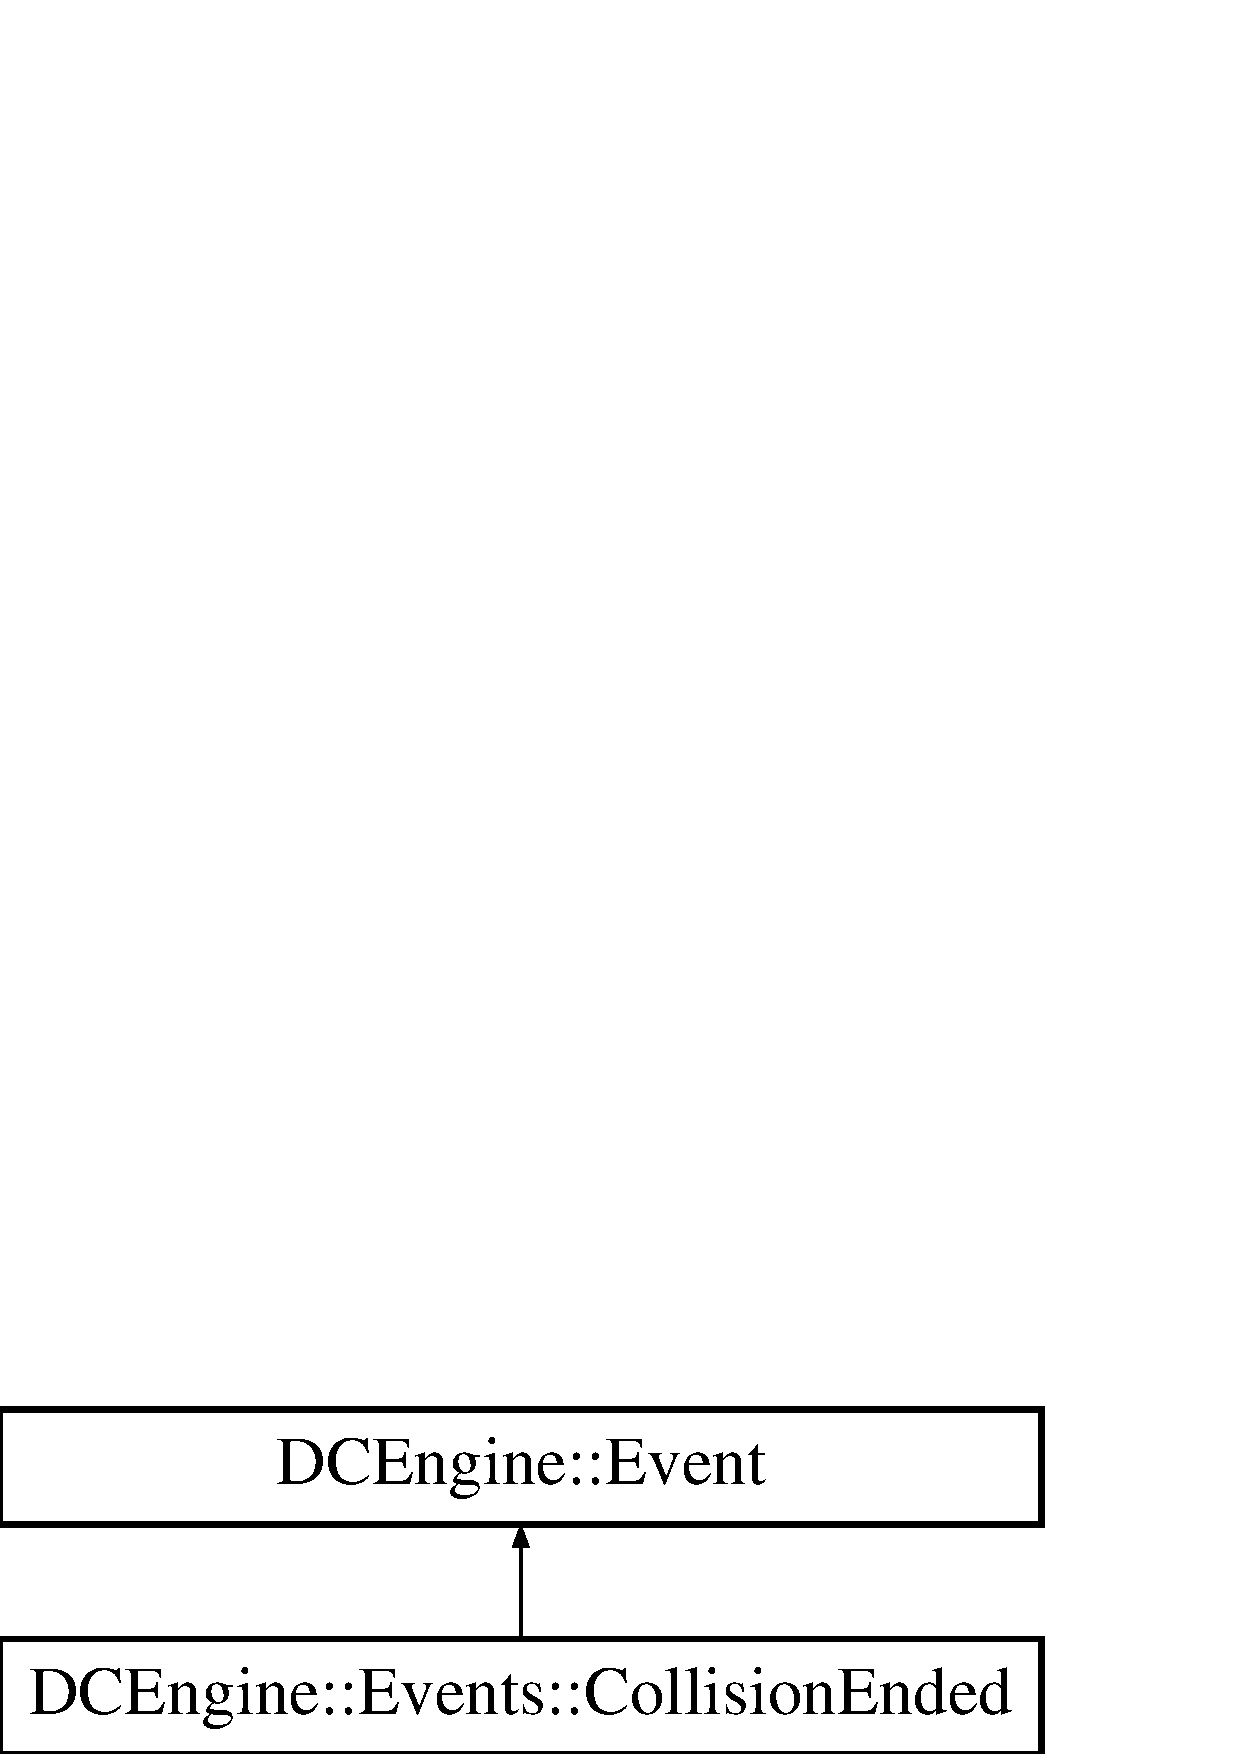
\includegraphics[height=2.000000cm]{classDCEngine_1_1Events_1_1CollisionEnded}
\end{center}
\end{figure}
\subsection*{Public Attributes}
\begin{DoxyCompactItemize}
\item 
\hypertarget{classDCEngine_1_1Events_1_1CollisionEnded_adc993f1e8a262271a68cdeedab678f6f}{\hyperlink{classDCEngine_1_1GameObject}{Game\-Object} $\ast$ \hyperlink{classDCEngine_1_1Events_1_1CollisionEnded_adc993f1e8a262271a68cdeedab678f6f}{Object}}\label{classDCEngine_1_1Events_1_1CollisionEnded_adc993f1e8a262271a68cdeedab678f6f}

\begin{DoxyCompactList}\small\item\em \hyperlink{classThe}{The} object this event was sent to. \end{DoxyCompactList}\item 
\hypertarget{classDCEngine_1_1Events_1_1CollisionEnded_a8681e405c6ad1ed260c6cef0ab4cae34}{\hyperlink{classDCEngine_1_1GameObject}{Game\-Object} $\ast$ \hyperlink{classDCEngine_1_1Events_1_1CollisionEnded_a8681e405c6ad1ed260c6cef0ab4cae34}{Other\-Object}}\label{classDCEngine_1_1Events_1_1CollisionEnded_a8681e405c6ad1ed260c6cef0ab4cae34}

\begin{DoxyCompactList}\small\item\em \hyperlink{classThe}{The} other object in the collision. \end{DoxyCompactList}\item 
\hypertarget{classDCEngine_1_1Events_1_1CollisionEnded_ad74e88ef2d614006ac1b8a6466f4a737}{Boolean {\bfseries Is\-Ghost}}\label{classDCEngine_1_1Events_1_1CollisionEnded_ad74e88ef2d614006ac1b8a6466f4a737}

\end{DoxyCompactItemize}
\subsection*{Additional Inherited Members}


The documentation for this class was generated from the following file\-:\begin{DoxyCompactItemize}
\item 
Core/\-Events/\hyperlink{CollisionEvents_8h}{Collision\-Events.\-h}\end{DoxyCompactItemize}

\hypertarget{structDCEngine_1_1CollisionFilter}{\section{D\-C\-Engine\-:\-:Collision\-Filter Struct Reference}
\label{structDCEngine_1_1CollisionFilter}\index{D\-C\-Engine\-::\-Collision\-Filter@{D\-C\-Engine\-::\-Collision\-Filter}}
}
\subsection*{Public Attributes}
\begin{DoxyCompactItemize}
\item 
\hypertarget{structDCEngine_1_1CollisionFilter_a2461259b77abd0b038f93900ffcf05d9}{std\-::pair$<$ std\-::string, \\*
std\-::string $>$ {\bfseries Pairing}}\label{structDCEngine_1_1CollisionFilter_a2461259b77abd0b038f93900ffcf05d9}

\item 
\hypertarget{structDCEngine_1_1CollisionFilter_affded1bf250f2b17612c2a2a9c46790b}{Collision\-Flag {\bfseries Collision\-Flag} = Collision\-Flag\-::\-Resolve}\label{structDCEngine_1_1CollisionFilter_affded1bf250f2b17612c2a2a9c46790b}

\item 
\hypertarget{structDCEngine_1_1CollisionFilter_ab5bd72452cd99e65a90fedb2e8a4ba69}{\hyperlink{structDCEngine_1_1CollisionBlock}{Collision\-Block} {\bfseries Collision\-Start\-Block}}\label{structDCEngine_1_1CollisionFilter_ab5bd72452cd99e65a90fedb2e8a4ba69}

\item 
\hypertarget{structDCEngine_1_1CollisionFilter_a333d84010f1c6d745fbcde0fe722cf5a}{\hyperlink{structDCEngine_1_1CollisionBlock}{Collision\-Block} {\bfseries Collision\-End\-Block}}\label{structDCEngine_1_1CollisionFilter_a333d84010f1c6d745fbcde0fe722cf5a}

\item 
\hypertarget{structDCEngine_1_1CollisionFilter_af0d6a8c4f729fd25ad52f06a2b95db2c}{\hyperlink{structDCEngine_1_1CollisionBlock}{Collision\-Block} {\bfseries Pre\-Solve\-Block}}\label{structDCEngine_1_1CollisionFilter_af0d6a8c4f729fd25ad52f06a2b95db2c}

\end{DoxyCompactItemize}


The documentation for this struct was generated from the following file\-:\begin{DoxyCompactItemize}
\item 
Core/\-Resources/\hyperlink{CollisionTable_8h}{Collision\-Table.\-h}\end{DoxyCompactItemize}

\hypertarget{classDCEngine_1_1CollisionGroup}{\section{D\-C\-Engine\-:\-:Collision\-Group Class Reference}
\label{classDCEngine_1_1CollisionGroup}\index{D\-C\-Engine\-::\-Collision\-Group@{D\-C\-Engine\-::\-Collision\-Group}}
}
Inheritance diagram for D\-C\-Engine\-:\-:Collision\-Group\-:\begin{figure}[H]
\begin{center}
\leavevmode
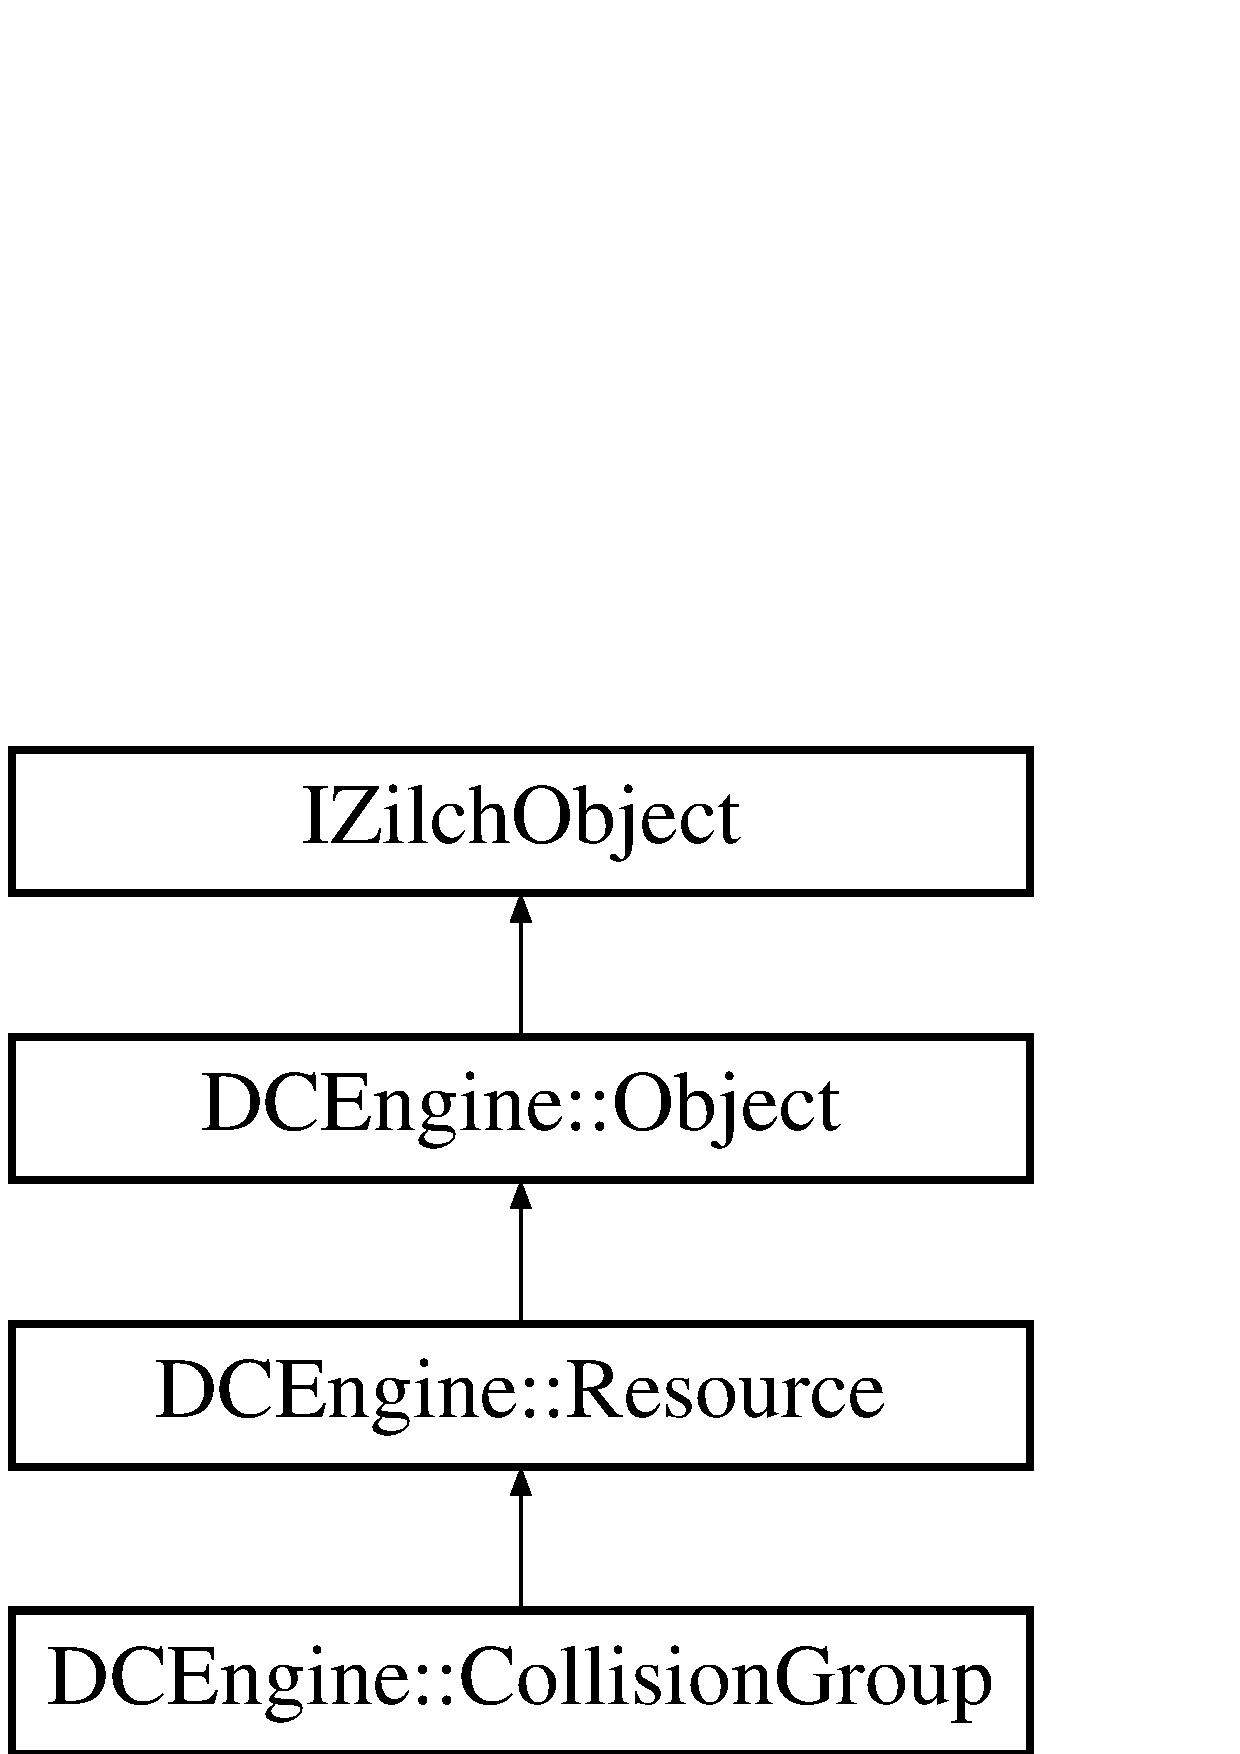
\includegraphics[height=4.000000cm]{classDCEngine_1_1CollisionGroup}
\end{center}
\end{figure}
\subsection*{Public Member Functions}
\begin{DoxyCompactItemize}
\item 
\hypertarget{classDCEngine_1_1CollisionGroup_adf82d868b8807935550230d9371c1d3c}{{\bfseries Zilch\-Declare\-Derived\-Type} (\hyperlink{classDCEngine_1_1CollisionGroup}{Collision\-Group}, \hyperlink{classDCEngine_1_1Resource}{Resource})}\label{classDCEngine_1_1CollisionGroup_adf82d868b8807935550230d9371c1d3c}

\item 
\hypertarget{classDCEngine_1_1CollisionGroup_a0b082f8e2eef665a4a64cd64ab2ace70}{\hyperlink{classDCEngine_1_1CollisionGroup_a0b082f8e2eef665a4a64cd64ab2ace70}{Collision\-Group} (std\-::string name)}\label{classDCEngine_1_1CollisionGroup_a0b082f8e2eef665a4a64cd64ab2ace70}

\begin{DoxyCompactList}\small\item\em \hyperlink{classDCEngine_1_1CollisionGroup}{Collision\-Group} constructor. \end{DoxyCompactList}\item 
\hypertarget{classDCEngine_1_1CollisionGroup_ad0f15f2c90e99ec60cdad4dd8d96b9b5}{\hyperlink{classDCEngine_1_1CollisionGroup}{Collision\-Group} \& {\bfseries operator=} (const \hyperlink{classDCEngine_1_1CollisionGroup}{Collision\-Group} \&rhs)}\label{classDCEngine_1_1CollisionGroup_ad0f15f2c90e99ec60cdad4dd8d96b9b5}

\end{DoxyCompactItemize}
\subsection*{Static Public Member Functions}
\begin{DoxyCompactItemize}
\item 
\hypertarget{classDCEngine_1_1CollisionGroup_afcace522fd707ff102c98070b881f6be}{static std\-::string {\bfseries Extension} ()}\label{classDCEngine_1_1CollisionGroup_afcace522fd707ff102c98070b881f6be}

\item 
static Collision\-Group\-Ptr \hyperlink{classDCEngine_1_1CollisionGroup_a9fc1343a6f3acbfeb9b0581628ad1dfb}{Find} (std\-::string)
\begin{DoxyCompactList}\small\item\em Returns the texture resource to be used by the graphics system. \end{DoxyCompactList}\end{DoxyCompactItemize}
\subsection*{Additional Inherited Members}


\subsection{Member Function Documentation}
\hypertarget{classDCEngine_1_1CollisionGroup_a9fc1343a6f3acbfeb9b0581628ad1dfb}{\index{D\-C\-Engine\-::\-Collision\-Group@{D\-C\-Engine\-::\-Collision\-Group}!Find@{Find}}
\index{Find@{Find}!DCEngine::CollisionGroup@{D\-C\-Engine\-::\-Collision\-Group}}
\subsubsection[{Find}]{\setlength{\rightskip}{0pt plus 5cm}Collision\-Group\-Ptr D\-C\-Engine\-::\-Collision\-Group\-::\-Find (
\begin{DoxyParamCaption}
\item[{std\-::string}]{name}
\end{DoxyParamCaption}
)\hspace{0.3cm}{\ttfamily [static]}}}\label{classDCEngine_1_1CollisionGroup_a9fc1343a6f3acbfeb9b0581628ad1dfb}


Returns the texture resource to be used by the graphics system. 

\begin{DoxyReturn}{Returns}
\hyperlink{classA}{A} reference to the texture object. 
\end{DoxyReturn}


The documentation for this class was generated from the following files\-:\begin{DoxyCompactItemize}
\item 
Core/\-Resources/\hyperlink{CollisionGroup_8h}{Collision\-Group.\-h}\item 
Core/\-Resources/\hyperlink{CollisionGroup_8cpp}{Collision\-Group.\-cpp}\end{DoxyCompactItemize}

\hypertarget{classDCEngine_1_1Events_1_1CollisionPersisted}{\section{D\-C\-Engine\-:\-:Events\-:\-:Collision\-Persisted Class Reference}
\label{classDCEngine_1_1Events_1_1CollisionPersisted}\index{D\-C\-Engine\-::\-Events\-::\-Collision\-Persisted@{D\-C\-Engine\-::\-Events\-::\-Collision\-Persisted}}
}
Inheritance diagram for D\-C\-Engine\-:\-:Events\-:\-:Collision\-Persisted\-:\begin{figure}[H]
\begin{center}
\leavevmode
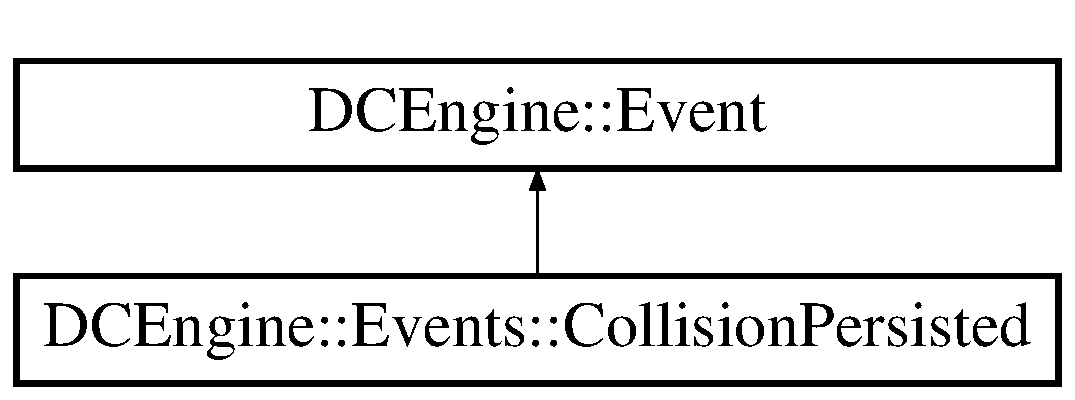
\includegraphics[height=2.000000cm]{classDCEngine_1_1Events_1_1CollisionPersisted}
\end{center}
\end{figure}
\subsection*{Public Attributes}
\begin{DoxyCompactItemize}
\item 
\hypertarget{classDCEngine_1_1Events_1_1CollisionPersisted_af3649bcb299ae8b07a1cb6cfb491727a}{\hyperlink{classDCEngine_1_1GameObject}{Game\-Object} $\ast$ \hyperlink{classDCEngine_1_1Events_1_1CollisionPersisted_af3649bcb299ae8b07a1cb6cfb491727a}{Object}}\label{classDCEngine_1_1Events_1_1CollisionPersisted_af3649bcb299ae8b07a1cb6cfb491727a}

\begin{DoxyCompactList}\small\item\em \hyperlink{classThe}{The} object this event was sent to. \end{DoxyCompactList}\item 
\hypertarget{classDCEngine_1_1Events_1_1CollisionPersisted_aec11577b5ecd7642ac94ef22246e5845}{\hyperlink{classDCEngine_1_1GameObject}{Game\-Object} $\ast$ \hyperlink{classDCEngine_1_1Events_1_1CollisionPersisted_aec11577b5ecd7642ac94ef22246e5845}{Other\-Object}}\label{classDCEngine_1_1Events_1_1CollisionPersisted_aec11577b5ecd7642ac94ef22246e5845}

\begin{DoxyCompactList}\small\item\em \hyperlink{classThe}{The} other object in the collision. \end{DoxyCompactList}\item 
\hypertarget{classDCEngine_1_1Events_1_1CollisionPersisted_a4bfcd4094f539ad601f10e91156ba1da}{Boolean {\bfseries Is\-Ghost}}\label{classDCEngine_1_1Events_1_1CollisionPersisted_a4bfcd4094f539ad601f10e91156ba1da}

\end{DoxyCompactItemize}
\subsection*{Additional Inherited Members}


The documentation for this class was generated from the following file\-:\begin{DoxyCompactItemize}
\item 
Core/\-Events/\hyperlink{CollisionEvents_8h}{Collision\-Events.\-h}\end{DoxyCompactItemize}

\hypertarget{classDCEngine_1_1Events_1_1CollisionStarted}{\section{D\-C\-Engine\-:\-:Events\-:\-:Collision\-Started Class Reference}
\label{classDCEngine_1_1Events_1_1CollisionStarted}\index{D\-C\-Engine\-::\-Events\-::\-Collision\-Started@{D\-C\-Engine\-::\-Events\-::\-Collision\-Started}}
}
Inheritance diagram for D\-C\-Engine\-:\-:Events\-:\-:Collision\-Started\-:\begin{figure}[H]
\begin{center}
\leavevmode
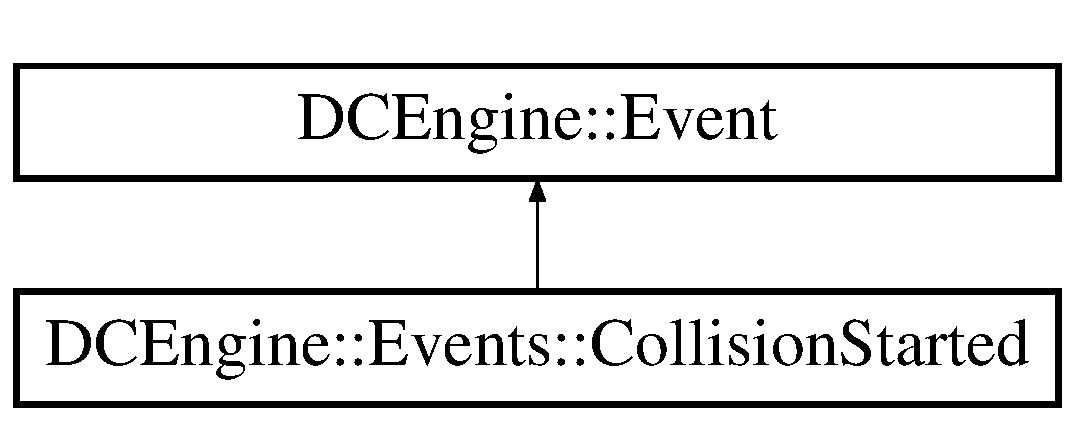
\includegraphics[height=2.000000cm]{classDCEngine_1_1Events_1_1CollisionStarted}
\end{center}
\end{figure}
\subsection*{Public Attributes}
\begin{DoxyCompactItemize}
\item 
\hypertarget{classDCEngine_1_1Events_1_1CollisionStarted_ae4c537e885960248e5b4dd7ad4fee960}{\hyperlink{classDCEngine_1_1GameObject}{Game\-Object} $\ast$ \hyperlink{classDCEngine_1_1Events_1_1CollisionStarted_ae4c537e885960248e5b4dd7ad4fee960}{Object}}\label{classDCEngine_1_1Events_1_1CollisionStarted_ae4c537e885960248e5b4dd7ad4fee960}

\begin{DoxyCompactList}\small\item\em \hyperlink{classThe}{The} object this event was sent to. \end{DoxyCompactList}\item 
\hypertarget{classDCEngine_1_1Events_1_1CollisionStarted_a39289bb67767390f168e894b9574cd1f}{\hyperlink{classDCEngine_1_1GameObject}{Game\-Object} $\ast$ \hyperlink{classDCEngine_1_1Events_1_1CollisionStarted_a39289bb67767390f168e894b9574cd1f}{Other\-Object}}\label{classDCEngine_1_1Events_1_1CollisionStarted_a39289bb67767390f168e894b9574cd1f}

\begin{DoxyCompactList}\small\item\em \hyperlink{classThe}{The} other object in the collision. \end{DoxyCompactList}\item 
\hypertarget{classDCEngine_1_1Events_1_1CollisionStarted_a7dcfe692c8ed8ef4237973973e617843}{Boolean {\bfseries Is\-Ghost}}\label{classDCEngine_1_1Events_1_1CollisionStarted_a7dcfe692c8ed8ef4237973973e617843}

\end{DoxyCompactItemize}
\subsection*{Additional Inherited Members}


The documentation for this class was generated from the following file\-:\begin{DoxyCompactItemize}
\item 
Core/\-Events/\hyperlink{CollisionEvents_8h}{Collision\-Events.\-h}\end{DoxyCompactItemize}

\hypertarget{classDCEngine_1_1CollisionTable}{\section{D\-C\-Engine\-:\-:Collision\-Table Class Reference}
\label{classDCEngine_1_1CollisionTable}\index{D\-C\-Engine\-::\-Collision\-Table@{D\-C\-Engine\-::\-Collision\-Table}}
}
Inheritance diagram for D\-C\-Engine\-:\-:Collision\-Table\-:\begin{figure}[H]
\begin{center}
\leavevmode
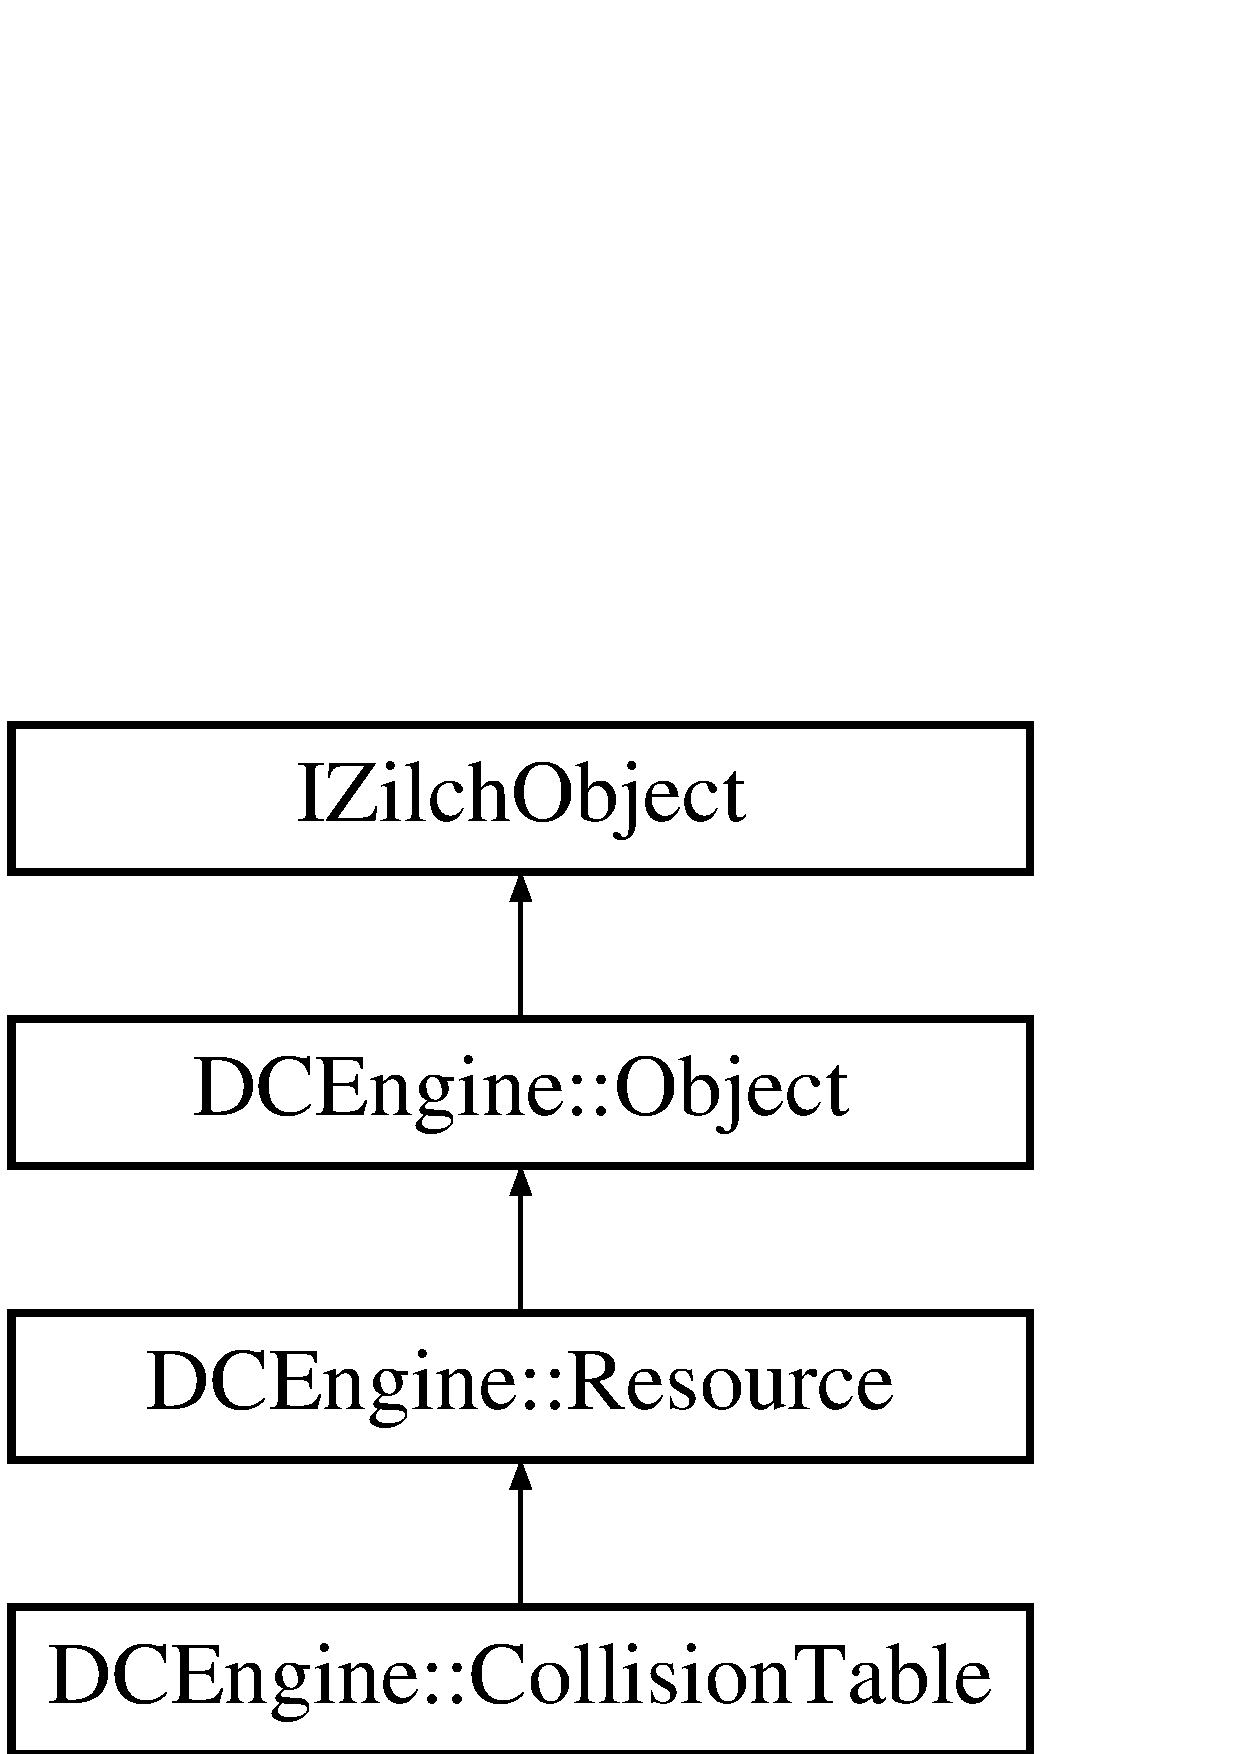
\includegraphics[height=4.000000cm]{classDCEngine_1_1CollisionTable}
\end{center}
\end{figure}
\subsection*{Public Member Functions}
\begin{DoxyCompactItemize}
\item 
\hypertarget{classDCEngine_1_1CollisionTable_a5e97da8fe9b4ea2844fe49226c9fe564}{{\bfseries Zilch\-Declare\-Derived\-Type} (\hyperlink{classDCEngine_1_1CollisionTable}{Collision\-Table}, \hyperlink{classDCEngine_1_1Resource}{Resource})}\label{classDCEngine_1_1CollisionTable_a5e97da8fe9b4ea2844fe49226c9fe564}

\item 
\hypertarget{classDCEngine_1_1CollisionTable_a8b62a793bbd367751a45cfcc2681b834}{\hyperlink{classDCEngine_1_1CollisionTable_a8b62a793bbd367751a45cfcc2681b834}{Collision\-Table} (std\-::string name)}\label{classDCEngine_1_1CollisionTable_a8b62a793bbd367751a45cfcc2681b834}

\begin{DoxyCompactList}\small\item\em \hyperlink{classDCEngine_1_1CollisionTable}{Collision\-Table} constructor. \end{DoxyCompactList}\item 
\hyperlink{classDCEngine_1_1CollisionTable_aa39e1b48c029c14459fe545bb97004ed}{Collision\-Table} (void)
\begin{DoxyCompactList}\small\item\em \hyperlink{classDCEngine_1_1CollisionTable}{Collision\-Table} constructor. \end{DoxyCompactList}\item 
\hypertarget{classDCEngine_1_1CollisionTable_a03ee6a3b44138f0cc82db5539f02c35e}{bool {\bfseries Add\-Group} (\hyperlink{classDCEngine_1_1CollisionGroup}{Collision\-Group} group)}\label{classDCEngine_1_1CollisionTable_a03ee6a3b44138f0cc82db5539f02c35e}

\item 
\hypertarget{classDCEngine_1_1CollisionTable_a55ea498c139389e534970c86f13aa48d}{bool {\bfseries Add\-Group} (std\-::string group)}\label{classDCEngine_1_1CollisionTable_a55ea498c139389e534970c86f13aa48d}

\item 
\hypertarget{classDCEngine_1_1CollisionTable_aac222f1ddf326d87651408f10e6b9b60}{std\-::vector$<$ \hyperlink{classDCEngine_1_1CollisionGroup}{Collision\-Group} $>$\\*
 const \& {\bfseries Get\-Groups} (void) const }\label{classDCEngine_1_1CollisionTable_aac222f1ddf326d87651408f10e6b9b60}

\item 
\hypertarget{classDCEngine_1_1CollisionTable_ac2ee42f0e29420cc36c2381c4ff05cf9}{std\-::vector$<$ \hyperlink{structDCEngine_1_1CollisionFilter}{Collision\-Filter} $>$\\*
 const \& {\bfseries Get\-Pairs} (void) const }\label{classDCEngine_1_1CollisionTable_ac2ee42f0e29420cc36c2381c4ff05cf9}

\item 
\hypertarget{classDCEngine_1_1CollisionTable_a7fafce069fa4dde57bf8391773fe5fb9}{\hyperlink{structDCEngine_1_1CollisionFilter}{Collision\-Filter} \& {\bfseries Get\-Filter} (std\-::string const \&group1, std\-::string const \&group2)}\label{classDCEngine_1_1CollisionTable_a7fafce069fa4dde57bf8391773fe5fb9}

\item 
\hypertarget{classDCEngine_1_1CollisionTable_aaf23fc16f950d66975522e6e75bb7781}{bool {\bfseries Set\-Resolve} (std\-::string const \&group1, std\-::string const \&group2, Collision\-Flag state)}\label{classDCEngine_1_1CollisionTable_aaf23fc16f950d66975522e6e75bb7781}

\item 
\hypertarget{classDCEngine_1_1CollisionTable_a4e03bd57335e21aa7258203c9e80ca10}{Collision\-Flag \& {\bfseries Get\-Resolve} (std\-::string const \&group1, std\-::string const \&group2)}\label{classDCEngine_1_1CollisionTable_a4e03bd57335e21aa7258203c9e80ca10}

\item 
\hypertarget{classDCEngine_1_1CollisionTable_a3e4235a3f5b7929a5a34db3b04664498}{bool {\bfseries Set\-Start\-Block} (std\-::string const \&group1, std\-::string const \&group2, \hyperlink{structDCEngine_1_1CollisionBlock}{Collision\-Block} state)}\label{classDCEngine_1_1CollisionTable_a3e4235a3f5b7929a5a34db3b04664498}

\item 
\hypertarget{classDCEngine_1_1CollisionTable_a80bb06a58421a3eb4d447f636cb6ccc0}{\hyperlink{structDCEngine_1_1CollisionBlock}{Collision\-Block} \& {\bfseries Get\-Start\-Block} (std\-::string const \&group1, std\-::string const \&group2)}\label{classDCEngine_1_1CollisionTable_a80bb06a58421a3eb4d447f636cb6ccc0}

\item 
\hypertarget{classDCEngine_1_1CollisionTable_aa646c40108e568a6136086b08cf6cdea}{bool {\bfseries Set\-End\-Block} (std\-::string const \&group1, std\-::string const \&group2, \hyperlink{structDCEngine_1_1CollisionBlock}{Collision\-Block} state)}\label{classDCEngine_1_1CollisionTable_aa646c40108e568a6136086b08cf6cdea}

\item 
\hypertarget{classDCEngine_1_1CollisionTable_ad20d1db90d96c45dd81855d158bfa0c8}{\hyperlink{structDCEngine_1_1CollisionBlock}{Collision\-Block} \& {\bfseries Get\-End\-Block} (std\-::string const \&group1, std\-::string const \&group2)}\label{classDCEngine_1_1CollisionTable_ad20d1db90d96c45dd81855d158bfa0c8}

\item 
\hypertarget{classDCEngine_1_1CollisionTable_a6ced5ff7731c9213bbe906fe49b49249}{bool {\bfseries Set\-Pre\-Solve\-Block} (std\-::string const \&group1, std\-::string const \&group2, \hyperlink{structDCEngine_1_1CollisionBlock}{Collision\-Block} state)}\label{classDCEngine_1_1CollisionTable_a6ced5ff7731c9213bbe906fe49b49249}

\item 
\hypertarget{classDCEngine_1_1CollisionTable_af484901e98e2e095275179d6da442208}{\hyperlink{structDCEngine_1_1CollisionBlock}{Collision\-Block} \& {\bfseries Get\-Pre\-Solve\-Block} (std\-::string const \&group1, std\-::string const \&group2)}\label{classDCEngine_1_1CollisionTable_af484901e98e2e095275179d6da442208}

\item 
\hypertarget{classDCEngine_1_1CollisionTable_a2ebb6549e1196033a3fc009e89b68bf5}{\hyperlink{classDCEngine_1_1CollisionTable}{Collision\-Table} \& {\bfseries operator=} (const \hyperlink{classDCEngine_1_1CollisionTable}{Collision\-Table} \&rhs)}\label{classDCEngine_1_1CollisionTable_a2ebb6549e1196033a3fc009e89b68bf5}

\end{DoxyCompactItemize}
\subsection*{Static Public Member Functions}
\begin{DoxyCompactItemize}
\item 
\hypertarget{classDCEngine_1_1CollisionTable_aad8cd32be9076a01c3a504fa7f2b8b29}{static std\-::string {\bfseries Extension} ()}\label{classDCEngine_1_1CollisionTable_aad8cd32be9076a01c3a504fa7f2b8b29}

\item 
\hypertarget{classDCEngine_1_1CollisionTable_a6e539c29d2880a2ecebba0fea92dc2ca}{static std\-::string {\bfseries Default} ()}\label{classDCEngine_1_1CollisionTable_a6e539c29d2880a2ecebba0fea92dc2ca}

\item 
static Collision\-Table\-Ptr \hyperlink{classDCEngine_1_1CollisionTable_a0f0c06d17cbb12699b923cdc70445db1}{Find} (std\-::string)
\begin{DoxyCompactList}\small\item\em Returns the texture resource to be used by the graphics system. \end{DoxyCompactList}\end{DoxyCompactItemize}
\subsection*{Additional Inherited Members}


\subsection{Constructor \& Destructor Documentation}
\hypertarget{classDCEngine_1_1CollisionTable_aa39e1b48c029c14459fe545bb97004ed}{\index{D\-C\-Engine\-::\-Collision\-Table@{D\-C\-Engine\-::\-Collision\-Table}!Collision\-Table@{Collision\-Table}}
\index{Collision\-Table@{Collision\-Table}!DCEngine::CollisionTable@{D\-C\-Engine\-::\-Collision\-Table}}
\subsubsection[{Collision\-Table}]{\setlength{\rightskip}{0pt plus 5cm}D\-C\-Engine\-::\-Collision\-Table\-::\-Collision\-Table (
\begin{DoxyParamCaption}
\item[{void}]{}
\end{DoxyParamCaption}
)}}\label{classDCEngine_1_1CollisionTable_aa39e1b48c029c14459fe545bb97004ed}


\hyperlink{classDCEngine_1_1CollisionTable}{Collision\-Table} constructor. 

\begin{DoxyRefDesc}{Todo}
\item[\hyperlink{todo__todo000008}{Todo}]What? Remove it. \end{DoxyRefDesc}


\subsection{Member Function Documentation}
\hypertarget{classDCEngine_1_1CollisionTable_a0f0c06d17cbb12699b923cdc70445db1}{\index{D\-C\-Engine\-::\-Collision\-Table@{D\-C\-Engine\-::\-Collision\-Table}!Find@{Find}}
\index{Find@{Find}!DCEngine::CollisionTable@{D\-C\-Engine\-::\-Collision\-Table}}
\subsubsection[{Find}]{\setlength{\rightskip}{0pt plus 5cm}Collision\-Table\-Ptr D\-C\-Engine\-::\-Collision\-Table\-::\-Find (
\begin{DoxyParamCaption}
\item[{std\-::string}]{name}
\end{DoxyParamCaption}
)\hspace{0.3cm}{\ttfamily [static]}}}\label{classDCEngine_1_1CollisionTable_a0f0c06d17cbb12699b923cdc70445db1}


Returns the texture resource to be used by the graphics system. 

\begin{DoxyReturn}{Returns}
\hyperlink{classA}{A} reference to the texture object. 
\end{DoxyReturn}


The documentation for this class was generated from the following files\-:\begin{DoxyCompactItemize}
\item 
Core/\-Resources/\hyperlink{CollisionTable_8h}{Collision\-Table.\-h}\item 
Core/\-Resources/\hyperlink{CollisionTable_8cpp}{Collision\-Table.\-cpp}\end{DoxyCompactItemize}

\hypertarget{classDCEngine_1_1Command}{\section{D\-C\-Engine\-:\-:Command Class Reference}
\label{classDCEngine_1_1Command}\index{D\-C\-Engine\-::\-Command@{D\-C\-Engine\-::\-Command}}
}
Inheritance diagram for D\-C\-Engine\-:\-:Command\-:\begin{figure}[H]
\begin{center}
\leavevmode
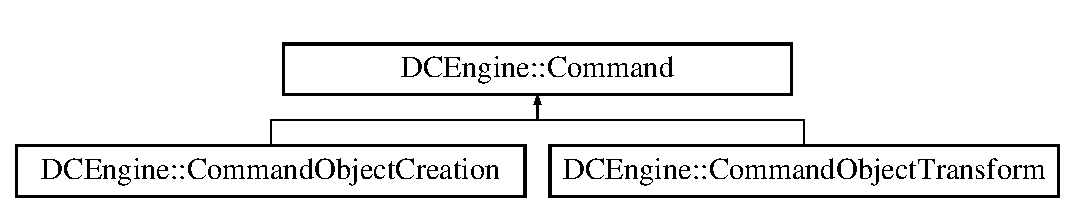
\includegraphics[height=2.000000cm]{classDCEngine_1_1Command}
\end{center}
\end{figure}
\subsection*{Public Member Functions}
\begin{DoxyCompactItemize}
\item 
\hypertarget{classDCEngine_1_1Command_aa35f7e42932a9d03da8df6add2a7c5d5}{{\bfseries Command} (std\-::string name)}\label{classDCEngine_1_1Command_aa35f7e42932a9d03da8df6add2a7c5d5}

\item 
\hypertarget{classDCEngine_1_1Command_a43a8d631d2b3a250a4e1c4192add7f70}{virtual void {\bfseries Undo} ()=0}\label{classDCEngine_1_1Command_a43a8d631d2b3a250a4e1c4192add7f70}

\item 
\hypertarget{classDCEngine_1_1Command_a5d2b11300b4cad6ddc245adaa87aa35a}{virtual void {\bfseries Execute} ()=0}\label{classDCEngine_1_1Command_a5d2b11300b4cad6ddc245adaa87aa35a}

\end{DoxyCompactItemize}
\subsection*{Public Attributes}
\begin{DoxyCompactItemize}
\item 
\hypertarget{classDCEngine_1_1Command_a03f72da121e2d28c0624958fdc85b19e}{std\-::string {\bfseries Command\-Name}}\label{classDCEngine_1_1Command_a03f72da121e2d28c0624958fdc85b19e}

\end{DoxyCompactItemize}


The documentation for this class was generated from the following file\-:\begin{DoxyCompactItemize}
\item 
Core/\-Engine/\hyperlink{Command_8h}{Command.\-h}\end{DoxyCompactItemize}

\hypertarget{classDCEngine_1_1CommandManager}{\section{D\-C\-Engine\-:\-:Command\-Manager Class Reference}
\label{classDCEngine_1_1CommandManager}\index{D\-C\-Engine\-::\-Command\-Manager@{D\-C\-Engine\-::\-Command\-Manager}}
}
\subsection*{Public Member Functions}
\begin{DoxyCompactItemize}
\item 
\hypertarget{classDCEngine_1_1CommandManager_ad3b0f61d5c1a06107f77d04b1b33d5a2}{\hyperlink{classDCEngine_1_1CommandManager_ad3b0f61d5c1a06107f77d04b1b33d5a2}{Command\-Manager} ()}\label{classDCEngine_1_1CommandManager_ad3b0f61d5c1a06107f77d04b1b33d5a2}

\begin{DoxyCompactList}\small\item\em \hyperlink{classDCEngine_1_1CommandManager}{Command\-Manager} constructor. \end{DoxyCompactList}\item 
void \hyperlink{classDCEngine_1_1CommandManager_a46efd76d37bc0754ec51aa835a810863}{Add} (Command\-Ptr command)
\begin{DoxyCompactList}\small\item\em Adds the latest command. \end{DoxyCompactList}\item 
\hypertarget{classDCEngine_1_1CommandManager_a67d0955255042f2185788896503da1ef}{void \hyperlink{classDCEngine_1_1CommandManager_a67d0955255042f2185788896503da1ef}{Undo} ()}\label{classDCEngine_1_1CommandManager_a67d0955255042f2185788896503da1ef}

\begin{DoxyCompactList}\small\item\em Undoes the last command. \end{DoxyCompactList}\item 
\hypertarget{classDCEngine_1_1CommandManager_afc5a4b8a89b9472bd2359cb023adc60a}{void \hyperlink{classDCEngine_1_1CommandManager_afc5a4b8a89b9472bd2359cb023adc60a}{Redo} ()}\label{classDCEngine_1_1CommandManager_afc5a4b8a89b9472bd2359cb023adc60a}

\begin{DoxyCompactList}\small\item\em Redoes the last command. \end{DoxyCompactList}\item 
\hypertarget{classDCEngine_1_1CommandManager_a16405d660e327349e83a43d7624e9424}{void {\bfseries Copy} (\hyperlink{classDCEngine_1_1GameObject}{Game\-Object} $\ast$)}\label{classDCEngine_1_1CommandManager_a16405d660e327349e83a43d7624e9424}

\item 
\hypertarget{classDCEngine_1_1CommandManager_ac9dfe330808b732d110001c243f7df78}{void {\bfseries Paste} (\hyperlink{classDCEngine_1_1Space}{Space} $\ast$)}\label{classDCEngine_1_1CommandManager_ac9dfe330808b732d110001c243f7df78}

\end{DoxyCompactItemize}
\subsection*{Public Attributes}
\begin{DoxyCompactItemize}
\item 
\hypertarget{classDCEngine_1_1CommandManager_a13b8ee1d816cca143d83adcbbd1e62fd}{std\-::deque$<$ Command\-Ptr $>$ {\bfseries Commands\-Current}}\label{classDCEngine_1_1CommandManager_a13b8ee1d816cca143d83adcbbd1e62fd}

\item 
\hypertarget{classDCEngine_1_1CommandManager_af0b0ea345851210427f08970ac1a309f}{std\-::deque$<$ Command\-Ptr $>$ {\bfseries Commands\-Undo}}\label{classDCEngine_1_1CommandManager_af0b0ea345851210427f08970ac1a309f}

\end{DoxyCompactItemize}


\subsection{Member Function Documentation}
\hypertarget{classDCEngine_1_1CommandManager_a46efd76d37bc0754ec51aa835a810863}{\index{D\-C\-Engine\-::\-Command\-Manager@{D\-C\-Engine\-::\-Command\-Manager}!Add@{Add}}
\index{Add@{Add}!DCEngine::CommandManager@{D\-C\-Engine\-::\-Command\-Manager}}
\subsubsection[{Add}]{\setlength{\rightskip}{0pt plus 5cm}void D\-C\-Engine\-::\-Command\-Manager\-::\-Add (
\begin{DoxyParamCaption}
\item[{Command\-Ptr}]{command}
\end{DoxyParamCaption}
)}}\label{classDCEngine_1_1CommandManager_a46efd76d37bc0754ec51aa835a810863}


Adds the latest command. 


\begin{DoxyParams}{Parameters}
{\em command} & \hyperlink{classA}{A} pointer to the latest command. \\
\hline
\end{DoxyParams}


The documentation for this class was generated from the following files\-:\begin{DoxyCompactItemize}
\item 
Core/\-Engine/\hyperlink{Command_8h}{Command.\-h}\item 
Core/\-Engine/\hyperlink{Command_8cpp}{Command.\-cpp}\end{DoxyCompactItemize}

\hypertarget{classDCEngine_1_1CommandObjectCreation}{\section{D\-C\-Engine\-:\-:Command\-Object\-Creation Class Reference}
\label{classDCEngine_1_1CommandObjectCreation}\index{D\-C\-Engine\-::\-Command\-Object\-Creation@{D\-C\-Engine\-::\-Command\-Object\-Creation}}
}
Inheritance diagram for D\-C\-Engine\-:\-:Command\-Object\-Creation\-:\begin{figure}[H]
\begin{center}
\leavevmode
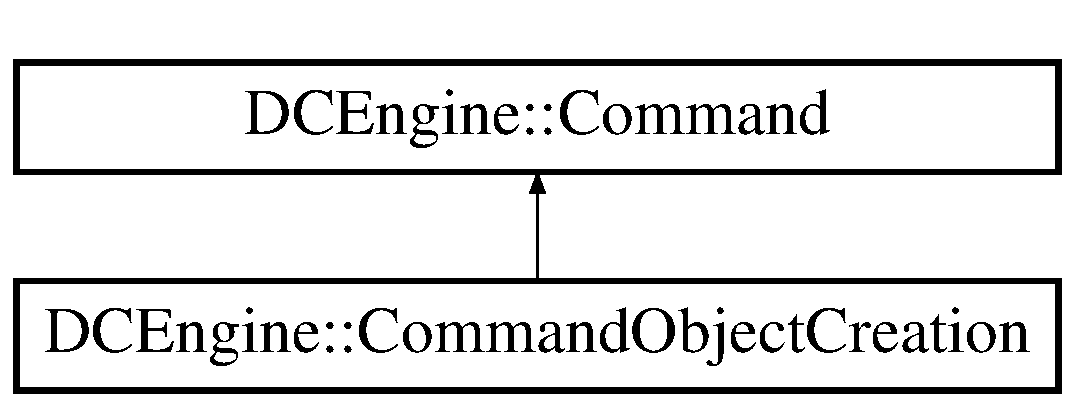
\includegraphics[height=2.000000cm]{classDCEngine_1_1CommandObjectCreation}
\end{center}
\end{figure}
\subsection*{Public Types}
\begin{DoxyCompactItemize}
\item 
enum {\bfseries Setting} \{ {\bfseries Create}, 
{\bfseries Destroy}
 \}
\end{DoxyCompactItemize}
\subsection*{Public Member Functions}
\begin{DoxyCompactItemize}
\item 
\hypertarget{classDCEngine_1_1CommandObjectCreation_aa6e8e01f3ea70b2257a319a7465e4839}{\hyperlink{classDCEngine_1_1CommandObjectCreation_aa6e8e01f3ea70b2257a319a7465e4839}{Command\-Object\-Creation} (\hyperlink{classDCEngine_1_1GameObject}{Game\-Object\-Ptr} game\-Object, \hyperlink{classDCEngine_1_1Space}{Space} $\ast$space, Setting setting)}\label{classDCEngine_1_1CommandObjectCreation_aa6e8e01f3ea70b2257a319a7465e4839}

\begin{DoxyCompactList}\small\item\em \hyperlink{classDCEngine_1_1CommandObjectCreation}{Command\-Object\-Creation} constructor. \end{DoxyCompactList}\item 
\hypertarget{classDCEngine_1_1CommandObjectCreation_a31ab1c485ccf5b416b1bf92f53d5521f}{{\bfseries Command\-Object\-Creation} (Game\-Object\-Raw\-Vec game\-Objects, \hyperlink{classDCEngine_1_1Space}{Space} $\ast$space, Setting setting)}\label{classDCEngine_1_1CommandObjectCreation_a31ab1c485ccf5b416b1bf92f53d5521f}

\item 
\hypertarget{classDCEngine_1_1CommandObjectCreation_a485481332df600dca540bcd11594be63}{{\bfseries Command\-Object\-Creation} (Archetype\-Container copy\-Data, \hyperlink{classDCEngine_1_1Space}{Space} $\ast$space)}\label{classDCEngine_1_1CommandObjectCreation_a485481332df600dca540bcd11594be63}

\item 
\hypertarget{classDCEngine_1_1CommandObjectCreation_af0a957acc7f80c247f26ea8421e5eb2f}{void \hyperlink{classDCEngine_1_1CommandObjectCreation_af0a957acc7f80c247f26ea8421e5eb2f}{Undo} ()}\label{classDCEngine_1_1CommandObjectCreation_af0a957acc7f80c247f26ea8421e5eb2f}

\begin{DoxyCompactList}\small\item\em Undoes the last Creation command, specific to the setting set. \end{DoxyCompactList}\item 
\hypertarget{classDCEngine_1_1CommandObjectCreation_aea823e7c160e8a09fb393459d7e2ff5d}{void \hyperlink{classDCEngine_1_1CommandObjectCreation_aea823e7c160e8a09fb393459d7e2ff5d}{Execute} ()}\label{classDCEngine_1_1CommandObjectCreation_aea823e7c160e8a09fb393459d7e2ff5d}

\begin{DoxyCompactList}\small\item\em Undoes the last Creation command, specific to the setting set. \end{DoxyCompactList}\item 
\hypertarget{classDCEngine_1_1CommandObjectCreation_ad76e4f90f29fe4bef214c624d2775dc9}{void \hyperlink{classDCEngine_1_1CommandObjectCreation_ad76e4f90f29fe4bef214c624d2775dc9}{Create} ()}\label{classDCEngine_1_1CommandObjectCreation_ad76e4f90f29fe4bef214c624d2775dc9}

\begin{DoxyCompactList}\small\item\em (Re)creates the Game\-Object(s). \end{DoxyCompactList}\item 
\hypertarget{classDCEngine_1_1CommandObjectCreation_aa12c1f9d71af2b76f6959129b74ea848}{void \hyperlink{classDCEngine_1_1CommandObjectCreation_aa12c1f9d71af2b76f6959129b74ea848}{Destroy} ()}\label{classDCEngine_1_1CommandObjectCreation_aa12c1f9d71af2b76f6959129b74ea848}

\begin{DoxyCompactList}\small\item\em Destroys the Game\-Objects. \end{DoxyCompactList}\item 
\hypertarget{classDCEngine_1_1CommandObjectCreation_ab54719033edf413729904e89a2bfacc1}{void \hyperlink{classDCEngine_1_1CommandObjectCreation_ab54719033edf413729904e89a2bfacc1}{Copy} ()}\label{classDCEngine_1_1CommandObjectCreation_ab54719033edf413729904e89a2bfacc1}

\begin{DoxyCompactList}\small\item\em Copies the \hyperlink{classDCEngine_1_1GameObject}{Game\-Object}'s data into an Archtype. \end{DoxyCompactList}\end{DoxyCompactItemize}
\subsection*{Public Attributes}
\begin{DoxyCompactItemize}
\item 
\hypertarget{classDCEngine_1_1CommandObjectCreation_a89067b099fcda02f3c2e6363df151f4e}{Setting {\bfseries Current\-Setting}}\label{classDCEngine_1_1CommandObjectCreation_a89067b099fcda02f3c2e6363df151f4e}

\item 
\hypertarget{classDCEngine_1_1CommandObjectCreation_a50e2a97172026832eed0c7ff22595e00}{\hyperlink{classDCEngine_1_1Space}{Space} $\ast$ {\bfseries Space\-Ref}}\label{classDCEngine_1_1CommandObjectCreation_a50e2a97172026832eed0c7ff22595e00}

\item 
\hypertarget{classDCEngine_1_1CommandObjectCreation_aa05e09aa8d81824ba2e00c1ad370043c}{Game\-Object\-Raw\-Vec {\bfseries Game\-Object\-References}}\label{classDCEngine_1_1CommandObjectCreation_aa05e09aa8d81824ba2e00c1ad370043c}

\item 
\hypertarget{classDCEngine_1_1CommandObjectCreation_a42c5414e7e6f75a54d9c2a800f4a7e9b}{Archetype\-Container {\bfseries Game\-Object\-Data}}\label{classDCEngine_1_1CommandObjectCreation_a42c5414e7e6f75a54d9c2a800f4a7e9b}

\end{DoxyCompactItemize}


The documentation for this class was generated from the following files\-:\begin{DoxyCompactItemize}
\item 
Core/\-Engine/\hyperlink{Command_8h}{Command.\-h}\item 
Core/\-Engine/\hyperlink{Command_8cpp}{Command.\-cpp}\end{DoxyCompactItemize}

\hypertarget{classDCEngine_1_1CommandObjectTransform}{\section{D\-C\-Engine\-:\-:Command\-Object\-Transform Class Reference}
\label{classDCEngine_1_1CommandObjectTransform}\index{D\-C\-Engine\-::\-Command\-Object\-Transform@{D\-C\-Engine\-::\-Command\-Object\-Transform}}
}
Inheritance diagram for D\-C\-Engine\-:\-:Command\-Object\-Transform\-:\begin{figure}[H]
\begin{center}
\leavevmode
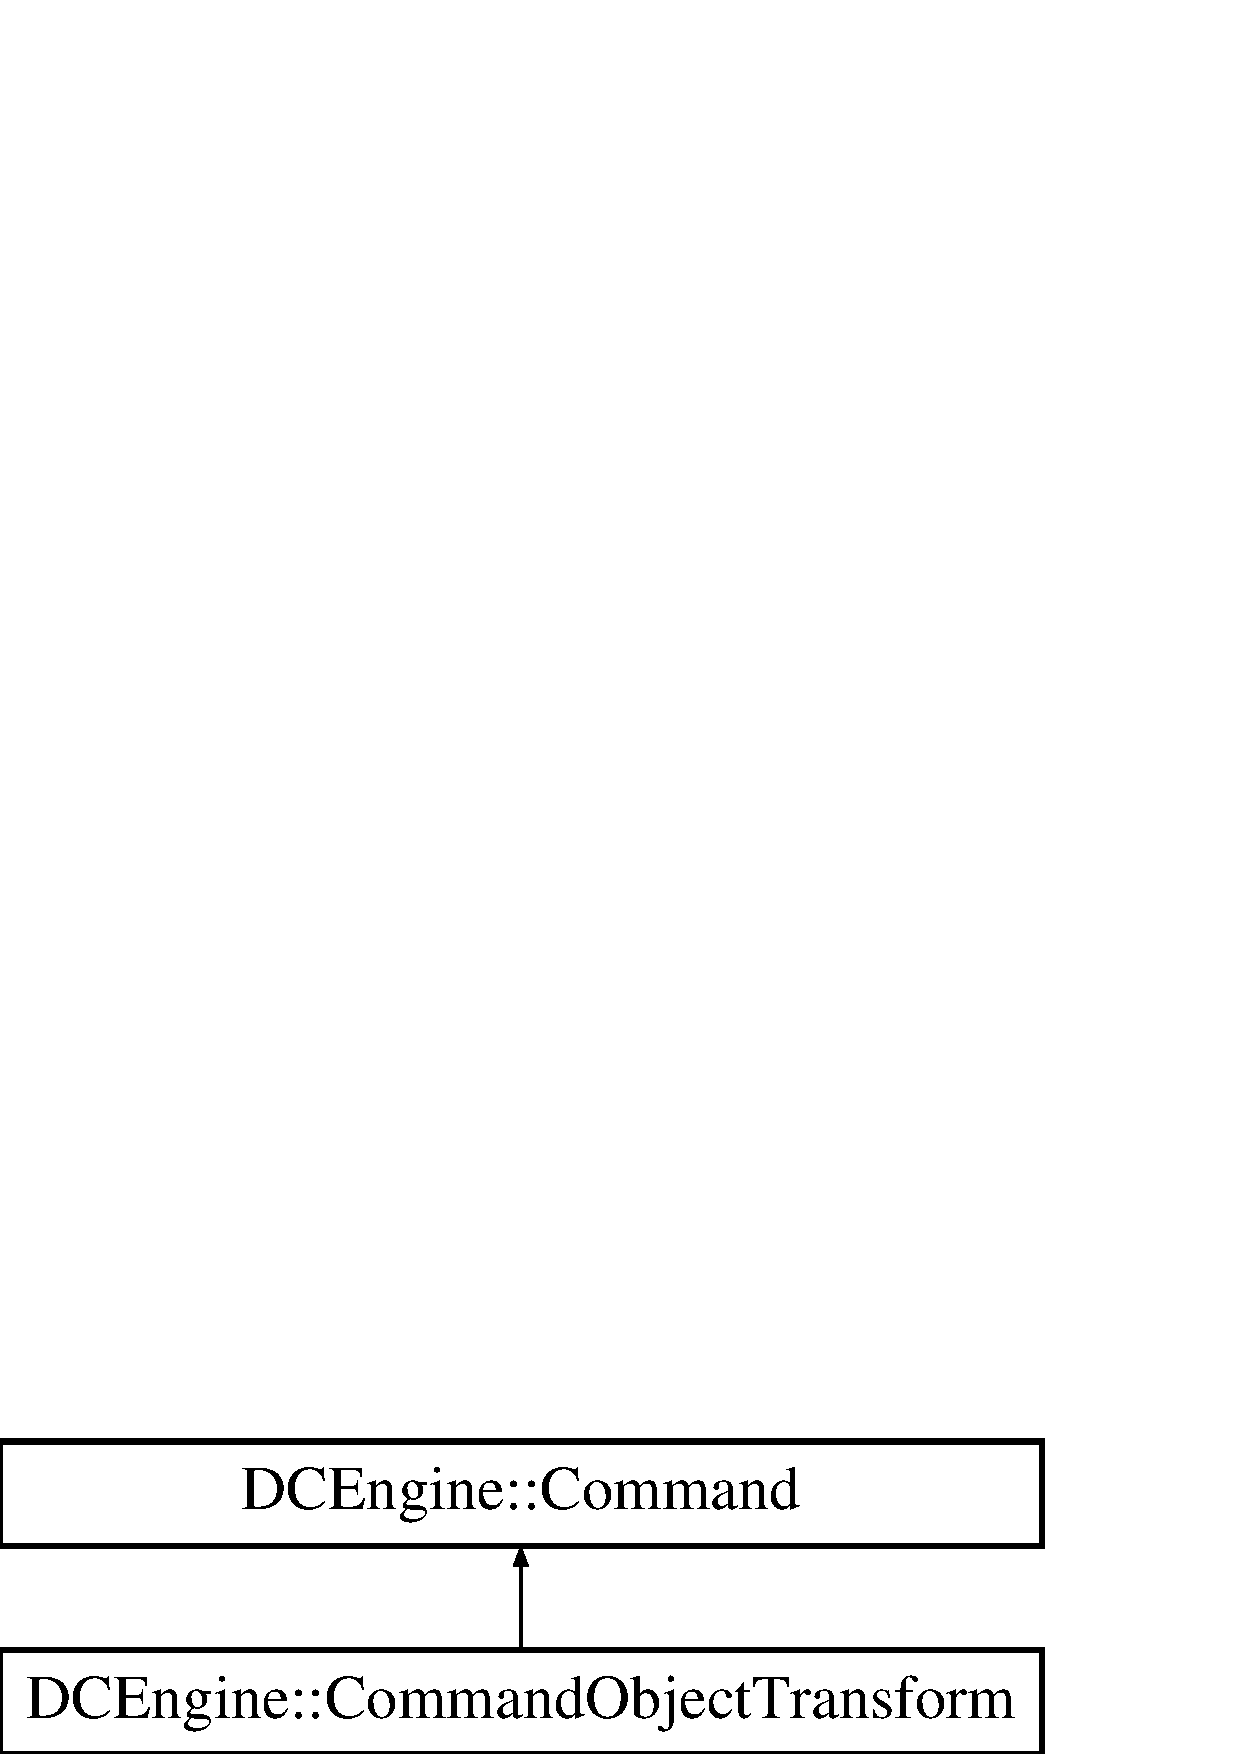
\includegraphics[height=2.000000cm]{classDCEngine_1_1CommandObjectTransform}
\end{center}
\end{figure}
\subsection*{Public Member Functions}
\begin{DoxyCompactItemize}
\item 
\hypertarget{classDCEngine_1_1CommandObjectTransform_af959e028016151f95d9e9c57dc26b437}{{\bfseries Command\-Object\-Transform} (\hyperlink{classDCEngine_1_1Components_1_1Transform}{Components\-::\-Transform} $\ast$transform)}\label{classDCEngine_1_1CommandObjectTransform_af959e028016151f95d9e9c57dc26b437}

\item 
\hypertarget{classDCEngine_1_1CommandObjectTransform_aa6578d45b3faf5cf8febeafcbf9af34f}{void {\bfseries Undo} ()}\label{classDCEngine_1_1CommandObjectTransform_aa6578d45b3faf5cf8febeafcbf9af34f}

\item 
\hypertarget{classDCEngine_1_1CommandObjectTransform_a97e768b53e6c225cac9e7820d196e10a}{void {\bfseries Execute} ()}\label{classDCEngine_1_1CommandObjectTransform_a97e768b53e6c225cac9e7820d196e10a}

\item 
\hypertarget{classDCEngine_1_1CommandObjectTransform_a274534c28f4f8a7a582860661096ba36}{void {\bfseries Save\-New} (Vec3 transform, Vec3 rotation, Vec3 scale)}\label{classDCEngine_1_1CommandObjectTransform_a274534c28f4f8a7a582860661096ba36}

\item 
\hypertarget{classDCEngine_1_1CommandObjectTransform_af869fe894d9b187617fc5f038806b16d}{void {\bfseries Save\-New} (\hyperlink{classDCEngine_1_1Components_1_1Transform}{Components\-::\-Transform} $\ast$transform)}\label{classDCEngine_1_1CommandObjectTransform_af869fe894d9b187617fc5f038806b16d}

\item 
\hypertarget{classDCEngine_1_1CommandObjectTransform_a422a74fcb39a80c039c851022c2b6ece}{void {\bfseries Save\-Previous} (Vec3 transform, Vec3 rotation, Vec3 scale)}\label{classDCEngine_1_1CommandObjectTransform_a422a74fcb39a80c039c851022c2b6ece}

\item 
\hypertarget{classDCEngine_1_1CommandObjectTransform_a6437a76ac47560d2d2ac4d4ea2e09b24}{void {\bfseries Save\-Previous} (\hyperlink{classDCEngine_1_1Components_1_1Transform}{Components\-::\-Transform} $\ast$transform)}\label{classDCEngine_1_1CommandObjectTransform_a6437a76ac47560d2d2ac4d4ea2e09b24}

\end{DoxyCompactItemize}
\subsection*{Public Attributes}
\begin{DoxyCompactItemize}
\item 
\hypertarget{classDCEngine_1_1CommandObjectTransform_a87af6501f861bf4a88f580c4d7b8db26}{\hyperlink{classDCEngine_1_1Components_1_1Transform}{Components\-::\-Transform} $\ast$ {\bfseries Transformed\-Object}}\label{classDCEngine_1_1CommandObjectTransform_a87af6501f861bf4a88f580c4d7b8db26}

\item 
\hypertarget{classDCEngine_1_1CommandObjectTransform_a08991276fe5d9d8423a8a8960d71fa5d}{Vec3 {\bfseries New\-Translation}}\label{classDCEngine_1_1CommandObjectTransform_a08991276fe5d9d8423a8a8960d71fa5d}

\item 
\hypertarget{classDCEngine_1_1CommandObjectTransform_afbca2f7afee9a8297fab5638e660c9b9}{Vec3 {\bfseries New\-Rotation}}\label{classDCEngine_1_1CommandObjectTransform_afbca2f7afee9a8297fab5638e660c9b9}

\item 
\hypertarget{classDCEngine_1_1CommandObjectTransform_ad3cfdcbd8f2ed5782c41e02db59115b1}{Vec3 {\bfseries New\-Scale}}\label{classDCEngine_1_1CommandObjectTransform_ad3cfdcbd8f2ed5782c41e02db59115b1}

\item 
\hypertarget{classDCEngine_1_1CommandObjectTransform_ad72961eae8d6afc5926ca421f27d2316}{Vec3 {\bfseries Previous\-Translation}}\label{classDCEngine_1_1CommandObjectTransform_ad72961eae8d6afc5926ca421f27d2316}

\item 
\hypertarget{classDCEngine_1_1CommandObjectTransform_ab7ea32692083790beb558a58e1f0c24c}{Vec3 {\bfseries Previous\-Rotation}}\label{classDCEngine_1_1CommandObjectTransform_ab7ea32692083790beb558a58e1f0c24c}

\item 
\hypertarget{classDCEngine_1_1CommandObjectTransform_a8ec66fcbfcb9d79a78edb70b1803012b}{Vec3 {\bfseries Previous\-Scale}}\label{classDCEngine_1_1CommandObjectTransform_a8ec66fcbfcb9d79a78edb70b1803012b}

\end{DoxyCompactItemize}


The documentation for this class was generated from the following files\-:\begin{DoxyCompactItemize}
\item 
Core/\-Engine/\hyperlink{Command_8h}{Command.\-h}\item 
Core/\-Engine/\hyperlink{Command_8cpp}{Command.\-cpp}\end{DoxyCompactItemize}

\hypertarget{classDCEngine_1_1Component}{\section{D\-C\-Engine\-:\-:Component Class Reference}
\label{classDCEngine_1_1Component}\index{D\-C\-Engine\-::\-Component@{D\-C\-Engine\-::\-Component}}
}
Inheritance diagram for D\-C\-Engine\-:\-:Component\-:\begin{figure}[H]
\begin{center}
\leavevmode
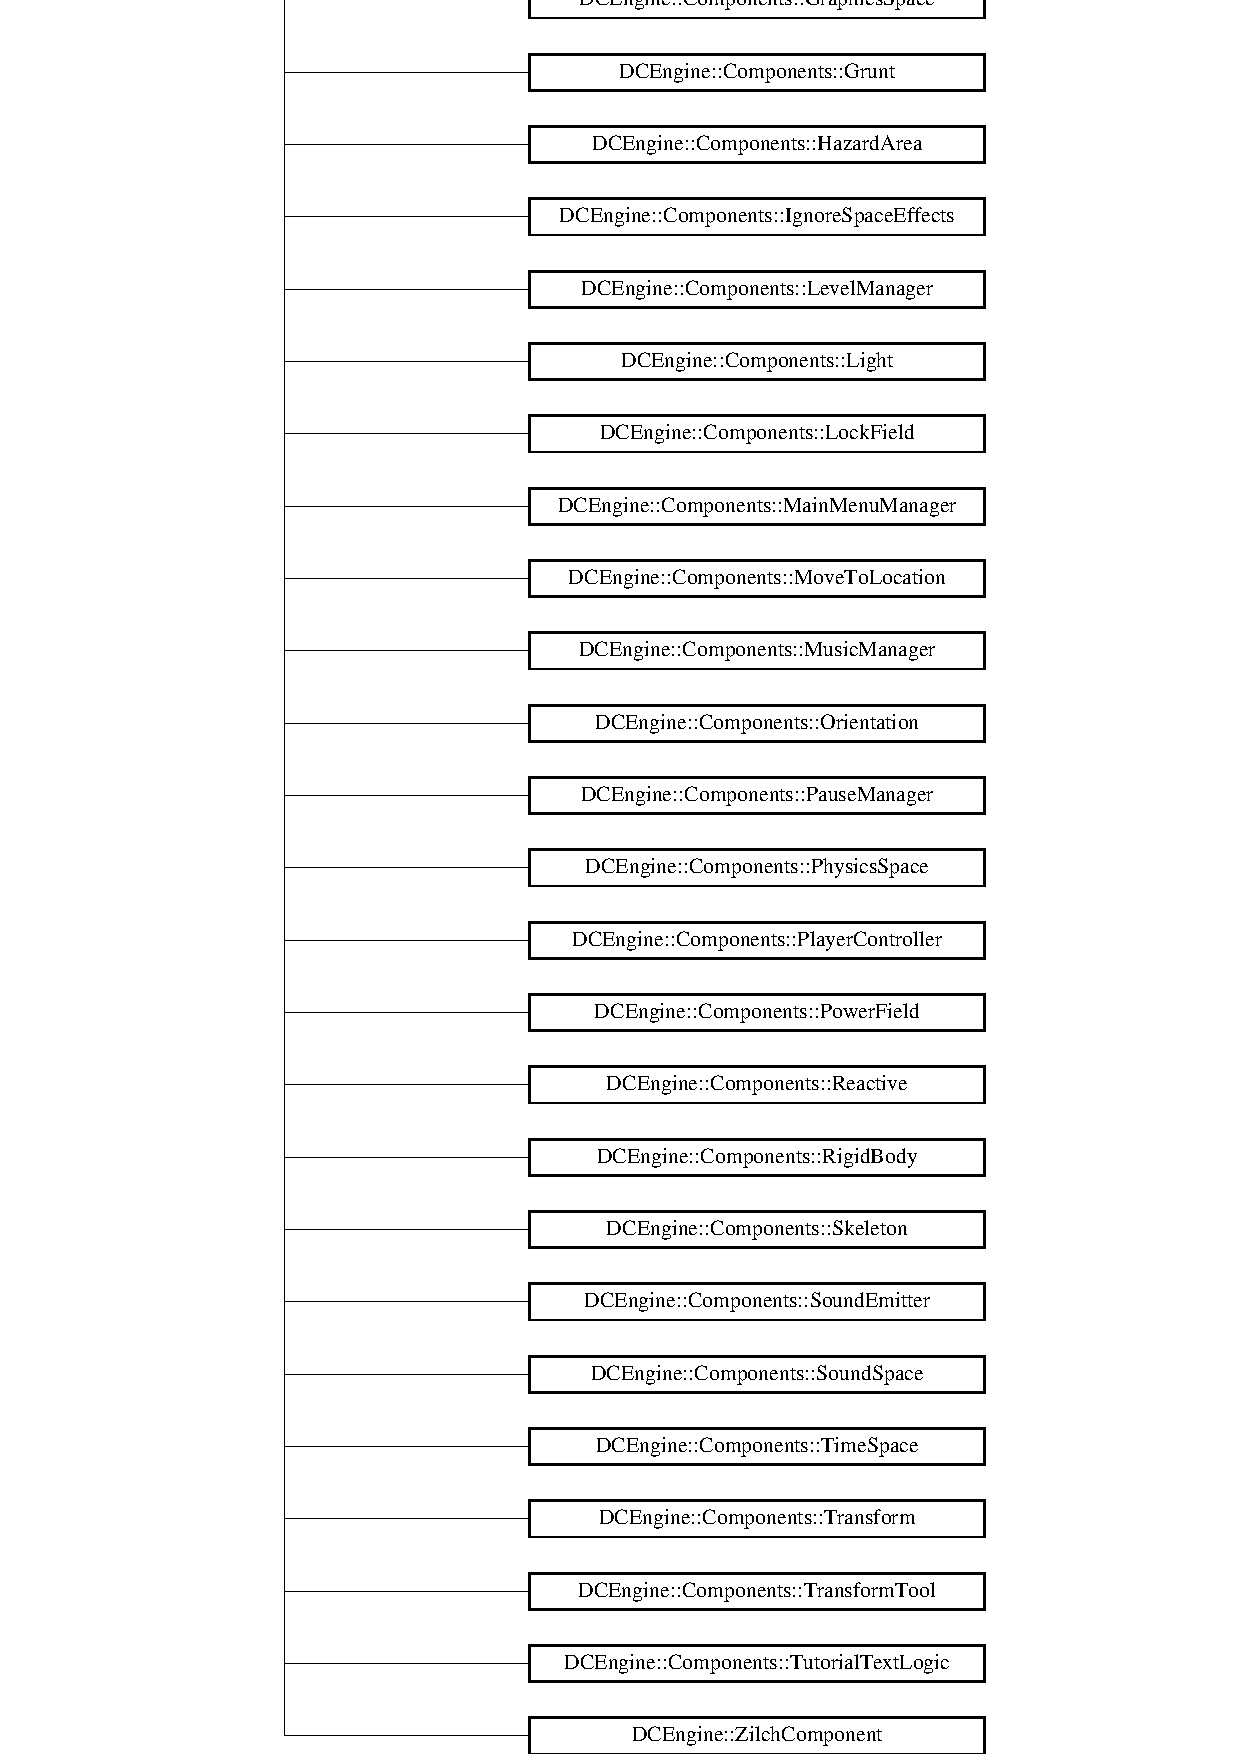
\includegraphics[height=12.000000cm]{classDCEngine_1_1Component}
\end{center}
\end{figure}
\subsection*{Public Member Functions}
\begin{DoxyCompactItemize}
\item 
\hypertarget{classDCEngine_1_1Component_a1d463d431a354f09864b0eb6dbce8ef2}{{\bfseries Zilch\-Declare\-Derived\-Type} (\hyperlink{classDCEngine_1_1Component}{Component}, \hyperlink{classDCEngine_1_1Object}{Object})}\label{classDCEngine_1_1Component_a1d463d431a354f09864b0eb6dbce8ef2}

\item 
\hypertarget{classDCEngine_1_1Component_a450b904300903683f54b2a2da772c485}{{\footnotesize template$<$typename Entity\-Class $>$ }\\Entity\-Class $\ast$ {\bfseries get\-Owner} ()}\label{classDCEngine_1_1Component_a450b904300903683f54b2a2da772c485}

\item 
\hyperlink{classDCEngine_1_1Entity}{Entity} $\ast$ \hyperlink{classDCEngine_1_1Component_ac294dc4c0ae2a6399bac40eef58287f7}{Owner} ()
\begin{DoxyCompactList}\small\item\em Returns a pointer to the \hyperlink{classDCEngine_1_1Entity}{Entity} that owns this component. \end{DoxyCompactList}\item 
\hypertarget{classDCEngine_1_1Component_a42de2ed8b4f78dbed97ef84ae84dbb8d}{const \hyperlink{classDCEngine_1_1Space}{Space} \& {\bfseries This\-Space} () const }\label{classDCEngine_1_1Component_a42de2ed8b4f78dbed97ef84ae84dbb8d}

\item 
\hypertarget{classDCEngine_1_1Component_ac236b6a79ede3fccdcbcd7774d6979f0}{const \hyperlink{classDCEngine_1_1GameSession}{Game\-Session} \& {\bfseries This\-Game\-Session} () const }\label{classDCEngine_1_1Component_ac236b6a79ede3fccdcbcd7774d6979f0}

\item 
\hypertarget{classDCEngine_1_1Component_a1b038e80a5b7786e8d3f4805351d56fc}{virtual Dependencies\-Container \& {\bfseries Dependencies} () const noexcept}\label{classDCEngine_1_1Component_a1b038e80a5b7786e8d3f4805351d56fc}

\item 
\hyperlink{classDCEngine_1_1Component_a74bd2d9c7b69be0c75322bc2ba496f88}{Component} (std\-::string name, \hyperlink{classDCEngine_1_1Entity}{Entity} \&owner)
\begin{DoxyCompactList}\small\item\em \hyperlink{classDCEngine_1_1Component}{Component} constructor. \end{DoxyCompactList}\item 
\hypertarget{classDCEngine_1_1Component_ac00f58512f2e5afa33f14007fd9c622e}{virtual \hyperlink{classDCEngine_1_1Component_ac00f58512f2e5afa33f14007fd9c622e}{$\sim$\-Component} ()}\label{classDCEngine_1_1Component_ac00f58512f2e5afa33f14007fd9c622e}

\begin{DoxyCompactList}\small\item\em \hyperlink{classDCEngine_1_1Component}{Component} destructor. \end{DoxyCompactList}\item 
\hypertarget{classDCEngine_1_1Component_a462cf1947b7d3f709c4825281623f05e}{virtual void {\bfseries Initialize} ()=0}\label{classDCEngine_1_1Component_a462cf1947b7d3f709c4825281623f05e}

\item 
\hypertarget{classDCEngine_1_1Component_af474d59bd4fe62ebff3fd2f308295a86}{void \hyperlink{classDCEngine_1_1Component_af474d59bd4fe62ebff3fd2f308295a86}{Destroy} ()}\label{classDCEngine_1_1Component_af474d59bd4fe62ebff3fd2f308295a86}

\begin{DoxyCompactList}\small\item\em Destroys the component at the beginning of the next frame. \end{DoxyCompactList}\item 
void \hyperlink{classDCEngine_1_1Component_a528b4171754da2aaf5ae2893c5fead7d}{Serialize} (Zilch\-::\-Json\-Builder \&builder)
\begin{DoxyCompactList}\small\item\em Serializes a \hyperlink{classDCEngine_1_1Component}{Component}. \end{DoxyCompactList}\item 
void \hyperlink{classDCEngine_1_1Component_ad1d066b15f0cf6094ff24fe53dea4ab7}{Deserialize} (Zilch\-::\-Json\-Value $\ast$properties)
\begin{DoxyCompactList}\small\item\em Deserializes a \hyperlink{classDCEngine_1_1Component}{Component}. \end{DoxyCompactList}\end{DoxyCompactItemize}
\subsection*{Static Public Member Functions}
\begin{DoxyCompactItemize}
\item 
static bool \hyperlink{classDCEngine_1_1Component_ac77fdca1c287921f639bcd93d43dc4c8}{Exists} (std\-::string component\-Name)
\begin{DoxyCompactList}\small\item\em Checks whether the component exists among the list of active components. \end{DoxyCompactList}\end{DoxyCompactItemize}
\subsection*{Public Attributes}
\begin{DoxyCompactItemize}
\item 
\hypertarget{classDCEngine_1_1Component_acdff26be1980d868761e54f32eea6219}{const unsigned int {\bfseries Component\-I\-D}}\label{classDCEngine_1_1Component_acdff26be1980d868761e54f32eea6219}

\end{DoxyCompactItemize}
\subsection*{Static Public Attributes}
\begin{DoxyCompactItemize}
\item 
\hypertarget{classDCEngine_1_1Component_a175738e900b11233bf516905797c23c7}{static unsigned int {\bfseries Components\-Created} = 0}\label{classDCEngine_1_1Component_a175738e900b11233bf516905797c23c7}

\item 
\hypertarget{classDCEngine_1_1Component_afe67576bb93cce3a053b1f8bb25e38ef}{static unsigned int {\bfseries Components\-Destroyed} = 0}\label{classDCEngine_1_1Component_afe67576bb93cce3a053b1f8bb25e38ef}

\item 
\hypertarget{classDCEngine_1_1Component_a839bb8cffb519b1570422772c791c26a}{static std\-::string {\bfseries Component\-Last\-Created}}\label{classDCEngine_1_1Component_a839bb8cffb519b1570422772c791c26a}

\item 
\hypertarget{classDCEngine_1_1Component_a9afe9259d705affe8d816d2f80407993}{static std\-::string {\bfseries Component\-Last\-Destroyed}}\label{classDCEngine_1_1Component_a9afe9259d705affe8d816d2f80407993}

\item 
\hypertarget{classDCEngine_1_1Component_a0d8174578805a0f8486a72d3cba36fb7}{static bool {\bfseries Diagnostics\-Enabled} = true}\label{classDCEngine_1_1Component_a0d8174578805a0f8486a72d3cba36fb7}

\end{DoxyCompactItemize}
\subsection*{Protected Types}
\begin{DoxyCompactItemize}
\item 
\hypertarget{classDCEngine_1_1Component_a7d6a7f58beccc0453b39d113f00f37c2}{using {\bfseries Dependencies\-Container} = std\-::vector$<$ std\-::string $>$}\label{classDCEngine_1_1Component_a7d6a7f58beccc0453b39d113f00f37c2}

\end{DoxyCompactItemize}
\subsection*{Protected Attributes}
\begin{DoxyCompactItemize}
\item 
\hypertarget{classDCEngine_1_1Component_a677bd02b725010574d579ff06082b08e}{\hyperlink{classDCEngine_1_1Space}{Space} $\ast$ {\bfseries Space\-Ref}}\label{classDCEngine_1_1Component_a677bd02b725010574d579ff06082b08e}

\item 
\hypertarget{classDCEngine_1_1Component_a5d0b8fc5b9696dba92667550fe3baa2e}{\hyperlink{classDCEngine_1_1GameSession}{Game\-Session} $\ast$ {\bfseries Game\-Session\-Ref}}\label{classDCEngine_1_1Component_a5d0b8fc5b9696dba92667550fe3baa2e}

\item 
\hypertarget{classDCEngine_1_1Component_ad1c8d9740f167555fd95004a8da73ac4}{std\-::vector$<$ \hyperlink{classDCEngine_1_1Entity}{Entity} $\ast$ $>$ {\bfseries Active\-Delegate\-Holders}}\label{classDCEngine_1_1Component_ad1c8d9740f167555fd95004a8da73ac4}

\end{DoxyCompactItemize}
\subsection*{Friends}
\begin{DoxyCompactItemize}
\item 
\hypertarget{classDCEngine_1_1Component_a614439ccac0344926adc4c0165d64060}{class {\bfseries Entity}}\label{classDCEngine_1_1Component_a614439ccac0344926adc4c0165d64060}

\item 
\hypertarget{classDCEngine_1_1Component_a00df87c957d8f7ee0fc51f07a0542f4a}{class {\bfseries Game\-Object}}\label{classDCEngine_1_1Component_a00df87c957d8f7ee0fc51f07a0542f4a}

\item 
\hypertarget{classDCEngine_1_1Component_a160097cc252ed86c269b6147933a7806}{class {\bfseries Systems\-::\-Factory}}\label{classDCEngine_1_1Component_a160097cc252ed86c269b6147933a7806}

\item 
\hypertarget{classDCEngine_1_1Component_a3e1914489e4bed4f9f23cdeab34a43dc}{class {\bfseries Engine}}\label{classDCEngine_1_1Component_a3e1914489e4bed4f9f23cdeab34a43dc}

\end{DoxyCompactItemize}
\subsection*{Additional Inherited Members}


\subsection{Constructor \& Destructor Documentation}
\hypertarget{classDCEngine_1_1Component_a74bd2d9c7b69be0c75322bc2ba496f88}{\index{D\-C\-Engine\-::\-Component@{D\-C\-Engine\-::\-Component}!Component@{Component}}
\index{Component@{Component}!DCEngine::Component@{D\-C\-Engine\-::\-Component}}
\subsubsection[{Component}]{\setlength{\rightskip}{0pt plus 5cm}D\-C\-Engine\-::\-Component\-::\-Component (
\begin{DoxyParamCaption}
\item[{std\-::string}]{name, }
\item[{{\bf Entity} \&}]{owner}
\end{DoxyParamCaption}
)}}\label{classDCEngine_1_1Component_a74bd2d9c7b69be0c75322bc2ba496f88}


\hyperlink{classDCEngine_1_1Component}{Component} constructor. 


\begin{DoxyParams}{Parameters}
{\em name} & \hyperlink{classThe}{The} name of the \hyperlink{classDCEngine_1_1Component}{Component} class. \\
\hline
{\em owner} & \hyperlink{classA}{A} reference to the \hyperlink{classDCEngine_1_1Entity}{Entity} that owns this component. \\
\hline
\end{DoxyParams}


\subsection{Member Function Documentation}
\hypertarget{classDCEngine_1_1Component_ad1d066b15f0cf6094ff24fe53dea4ab7}{\index{D\-C\-Engine\-::\-Component@{D\-C\-Engine\-::\-Component}!Deserialize@{Deserialize}}
\index{Deserialize@{Deserialize}!DCEngine::Component@{D\-C\-Engine\-::\-Component}}
\subsubsection[{Deserialize}]{\setlength{\rightskip}{0pt plus 5cm}void D\-C\-Engine\-::\-Component\-::\-Deserialize (
\begin{DoxyParamCaption}
\item[{Zilch\-::\-Json\-Value $\ast$}]{properties}
\end{DoxyParamCaption}
)}}\label{classDCEngine_1_1Component_ad1d066b15f0cf6094ff24fe53dea4ab7}


Deserializes a \hyperlink{classDCEngine_1_1Component}{Component}. 


\begin{DoxyParams}{Parameters}
{\em builder} & \hyperlink{classA}{A} pointer to the object containing the properties. \\
\hline
\end{DoxyParams}
\begin{DoxyNote}{Note}
This will deserialize the \hyperlink{classDCEngine_1_1Component}{Component}'s properties. 
\end{DoxyNote}
\hypertarget{classDCEngine_1_1Component_ac77fdca1c287921f639bcd93d43dc4c8}{\index{D\-C\-Engine\-::\-Component@{D\-C\-Engine\-::\-Component}!Exists@{Exists}}
\index{Exists@{Exists}!DCEngine::Component@{D\-C\-Engine\-::\-Component}}
\subsubsection[{Exists}]{\setlength{\rightskip}{0pt plus 5cm}bool D\-C\-Engine\-::\-Component\-::\-Exists (
\begin{DoxyParamCaption}
\item[{std\-::string}]{component\-Name}
\end{DoxyParamCaption}
)\hspace{0.3cm}{\ttfamily [static]}}}\label{classDCEngine_1_1Component_ac77fdca1c287921f639bcd93d43dc4c8}


Checks whether the component exists among the list of active components. 


\begin{DoxyParams}{Parameters}
{\em component\-Name} & \hyperlink{classThe}{The} name of the component. \\
\hline
\end{DoxyParams}
\begin{DoxyReturn}{Returns}
Whether the component exists among the list of created components. 
\end{DoxyReturn}
\hypertarget{classDCEngine_1_1Component_ac294dc4c0ae2a6399bac40eef58287f7}{\index{D\-C\-Engine\-::\-Component@{D\-C\-Engine\-::\-Component}!Owner@{Owner}}
\index{Owner@{Owner}!DCEngine::Component@{D\-C\-Engine\-::\-Component}}
\subsubsection[{Owner}]{\setlength{\rightskip}{0pt plus 5cm}{\bf Entity} $\ast$ D\-C\-Engine\-::\-Component\-::\-Owner (
\begin{DoxyParamCaption}
{}
\end{DoxyParamCaption}
)}}\label{classDCEngine_1_1Component_ac294dc4c0ae2a6399bac40eef58287f7}


Returns a pointer to the \hyperlink{classDCEngine_1_1Entity}{Entity} that owns this component. 

\begin{DoxyReturn}{Returns}
\hyperlink{classAn}{An} entity pointer. 
\end{DoxyReturn}
\hypertarget{classDCEngine_1_1Component_a528b4171754da2aaf5ae2893c5fead7d}{\index{D\-C\-Engine\-::\-Component@{D\-C\-Engine\-::\-Component}!Serialize@{Serialize}}
\index{Serialize@{Serialize}!DCEngine::Component@{D\-C\-Engine\-::\-Component}}
\subsubsection[{Serialize}]{\setlength{\rightskip}{0pt plus 5cm}void D\-C\-Engine\-::\-Component\-::\-Serialize (
\begin{DoxyParamCaption}
\item[{Zilch\-::\-Json\-Builder \&}]{builder}
\end{DoxyParamCaption}
)}}\label{classDCEngine_1_1Component_a528b4171754da2aaf5ae2893c5fead7d}


Serializes a \hyperlink{classDCEngine_1_1Component}{Component}. 


\begin{DoxyParams}{Parameters}
{\em builder} & \hyperlink{classA}{A} reference to the J\-S\-O\-N builder. \\
\hline
\end{DoxyParams}
\begin{DoxyNote}{Note}
This will serialize the component and all its properties. 
\end{DoxyNote}


The documentation for this class was generated from the following files\-:\begin{DoxyCompactItemize}
\item 
Core/\-Objects/\hyperlink{Component_8h}{Component.\-h}\item 
Core/\-Objects/Component.\-cpp\end{DoxyCompactItemize}

\hypertarget{classDCEngine_1_1Systems_1_1ComponentFactory}{\section{D\-C\-Engine\-:\-:Systems\-:\-:Component\-Factory$<$ Component\-Class $>$ Class Template Reference}
\label{classDCEngine_1_1Systems_1_1ComponentFactory}\index{D\-C\-Engine\-::\-Systems\-::\-Component\-Factory$<$ Component\-Class $>$@{D\-C\-Engine\-::\-Systems\-::\-Component\-Factory$<$ Component\-Class $>$}}
}
Inheritance diagram for D\-C\-Engine\-:\-:Systems\-:\-:Component\-Factory$<$ Component\-Class $>$\-:\begin{figure}[H]
\begin{center}
\leavevmode
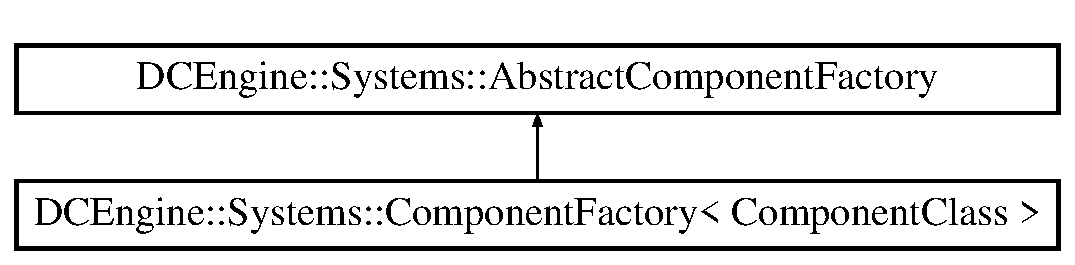
\includegraphics[height=2.000000cm]{classDCEngine_1_1Systems_1_1ComponentFactory}
\end{center}
\end{figure}
\subsection*{Public Member Functions}
\begin{DoxyCompactItemize}
\item 
\hypertarget{classDCEngine_1_1Systems_1_1ComponentFactory_acc8f00553bfcc6599c7b74a2f7b0a98a}{std\-::unique\-\_\-ptr$<$ \hyperlink{classDCEngine_1_1Component}{Component} $>$ {\bfseries Construct\-Component} (\hyperlink{classDCEngine_1_1Entity}{Entity} \&owner)}\label{classDCEngine_1_1Systems_1_1ComponentFactory_acc8f00553bfcc6599c7b74a2f7b0a98a}

\end{DoxyCompactItemize}


The documentation for this class was generated from the following file\-:\begin{DoxyCompactItemize}
\item 
Core/\-Systems/\-Factory/\hyperlink{ComponentFactory_8h}{Component\-Factory.\-h}\end{DoxyCompactItemize}

\hypertarget{structConfiguration}{\section{Configuration Struct Reference}
\label{structConfiguration}\index{Configuration@{Configuration}}
}


\subsection{Detailed Description}
the Editor system. 

The documentation for this struct was generated from the following file\-:\begin{DoxyCompactItemize}
\item 
Core/\-Systems/\-Editor/\hyperlink{Editor_8h}{Editor.\-h}\end{DoxyCompactItemize}

\hypertarget{classDCEngine_1_1Systems_1_1Content}{\section{D\-C\-Engine\-:\-:Systems\-:\-:Content Class Reference}
\label{classDCEngine_1_1Systems_1_1Content}\index{D\-C\-Engine\-::\-Systems\-::\-Content@{D\-C\-Engine\-::\-Systems\-::\-Content}}
}
Inheritance diagram for D\-C\-Engine\-:\-:Systems\-:\-:Content\-:\begin{figure}[H]
\begin{center}
\leavevmode
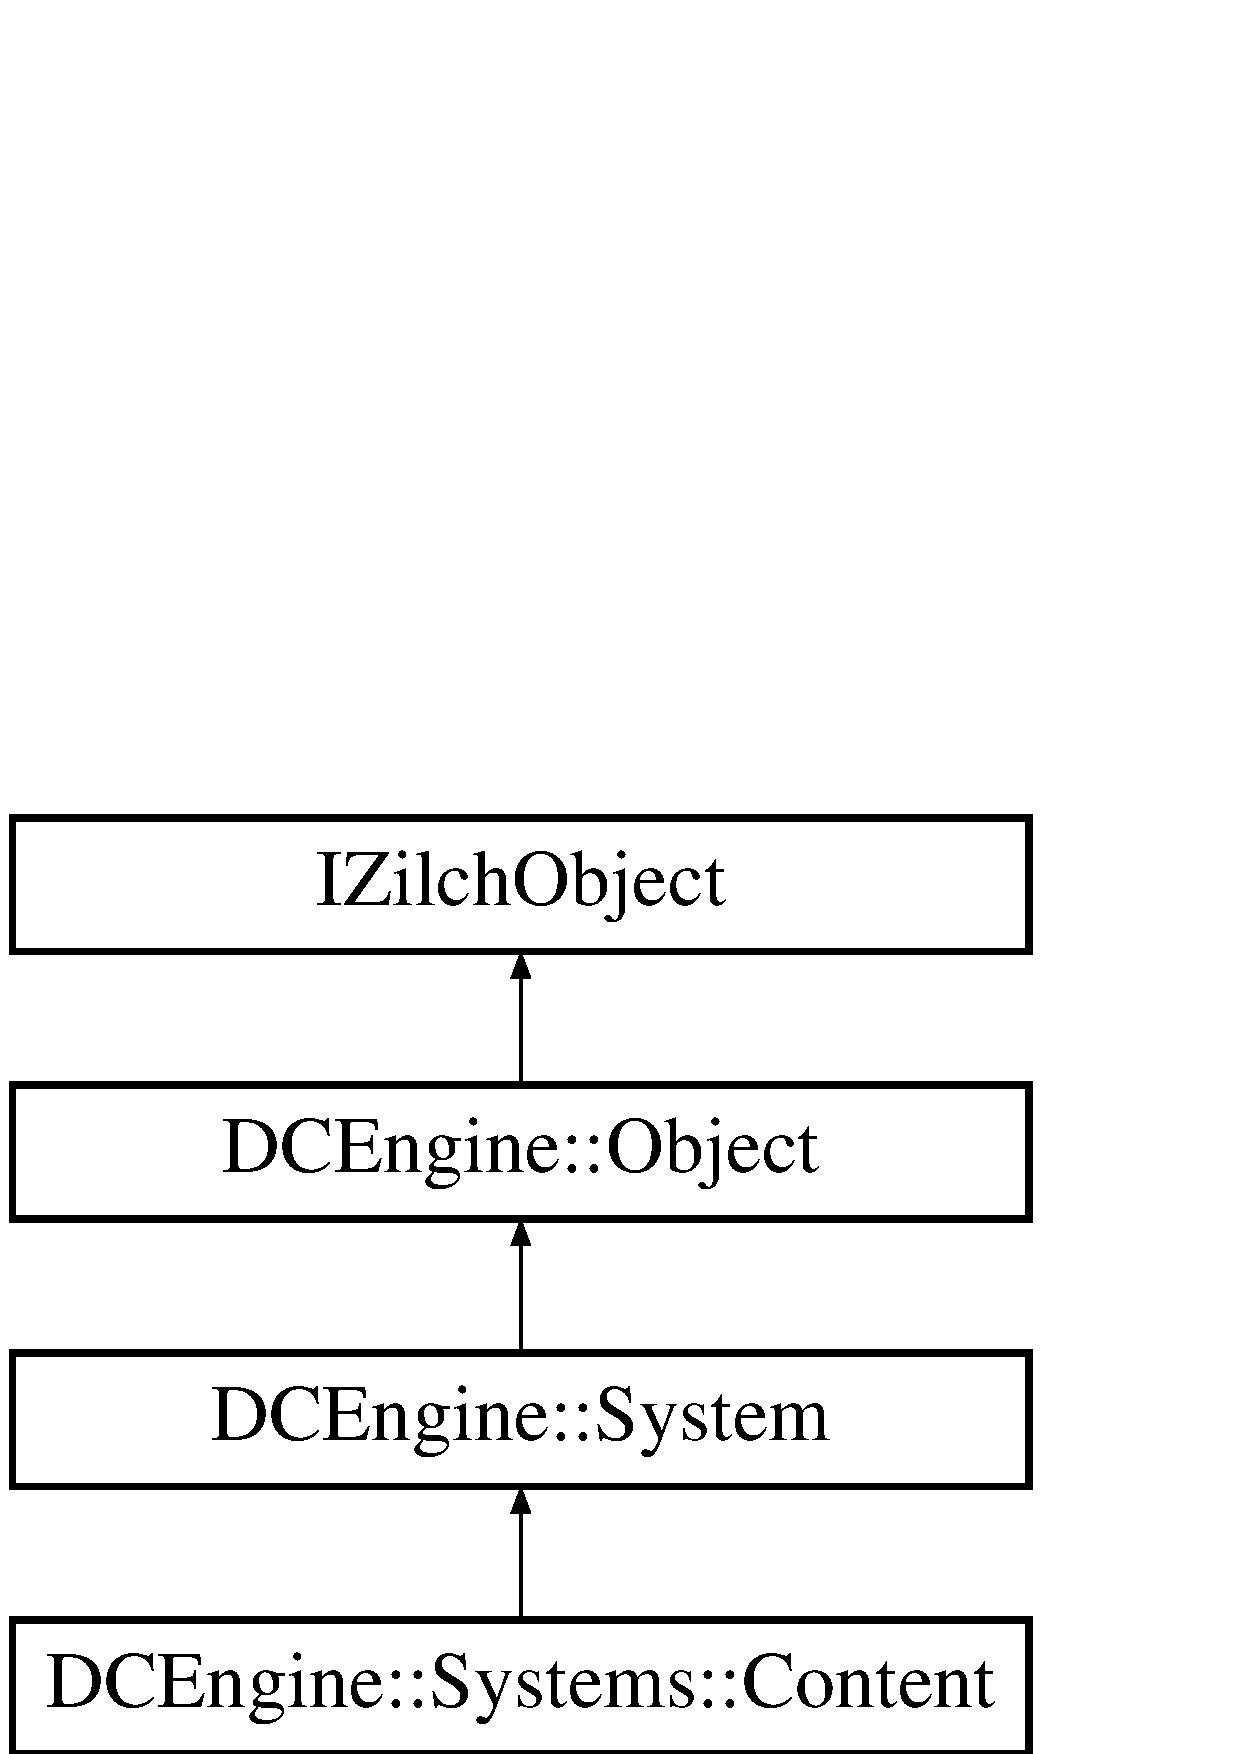
\includegraphics[height=4.000000cm]{classDCEngine_1_1Systems_1_1Content}
\end{center}
\end{figure}
\subsection*{Public Member Functions}
\begin{DoxyCompactItemize}
\item 
\hypertarget{classDCEngine_1_1Systems_1_1Content_a06ab0b01a39b528d99e94146c69bc62a}{void \hyperlink{classDCEngine_1_1Systems_1_1Content_a06ab0b01a39b528d99e94146c69bc62a}{Load\-Project\-Resources} ()}\label{classDCEngine_1_1Systems_1_1Content_a06ab0b01a39b528d99e94146c69bc62a}

\begin{DoxyCompactList}\small\item\em Load resources from a project. \end{DoxyCompactList}\item 
Bank\-Ptr \hyperlink{classDCEngine_1_1Systems_1_1Content_a9e7a6f2318997afd91906175307df4c6}{get\-Bank} (std\-::string bank\-Name)
\begin{DoxyCompactList}\small\item\em Grabs a \hyperlink{classDCEngine_1_1Bank}{Bank} resource. \end{DoxyCompactList}\item 
Shader\-Ptr \hyperlink{classDCEngine_1_1Systems_1_1Content_adc5229d03f74e7b3134f35e22341368e}{get\-Shader} (std\-::string shader\-Name)
\begin{DoxyCompactList}\small\item\em Grabs a shader resource. \end{DoxyCompactList}\item 
Font\-Ptr \hyperlink{classDCEngine_1_1Systems_1_1Content_a4103e542bf0efb910429a69b274a8634}{get\-Font} (std\-::string \&font\-Name)
\begin{DoxyCompactList}\small\item\em Grabs a font resource. \end{DoxyCompactList}\item 
Sprite\-Source\-Ptr \hyperlink{classDCEngine_1_1Systems_1_1Content_a01e53fe6a380629bc1200c01452c583a}{get\-Sprite\-Src} (std\-::string \&sprite\-Name)
\begin{DoxyCompactList}\small\item\em Grabs a \hyperlink{classDCEngine_1_1SpriteSource}{Sprite\-Source} resource. \end{DoxyCompactList}\item 
Sound\-Cue\-Ptr \hyperlink{classDCEngine_1_1Systems_1_1Content_ae0eb7e36feb5c793a0acefb204315c43}{get\-Sound\-Cue} (std\-::string \&sound\-Cue\-Name)
\begin{DoxyCompactList}\small\item\em Grabs a \hyperlink{classDCEngine_1_1SoundCue}{Sound\-Cue} resource. \end{DoxyCompactList}\item 
Archetype\-Ptr \hyperlink{classDCEngine_1_1Systems_1_1Content_a33344031ba414b7ee28e0c5f10f495f7}{get\-Archetype} (std\-::string \&archetype\-Name)
\begin{DoxyCompactList}\small\item\em Grabs an \hyperlink{classDCEngine_1_1Archetype}{Archetype} resource. \end{DoxyCompactList}\item 
Level\-Ptr \hyperlink{classDCEngine_1_1Systems_1_1Content_ad62d0bedd6cb8a96dd49278a24c875e5}{get\-Level} (std\-::string \&level\-Name)
\begin{DoxyCompactList}\small\item\em Grabs a \hyperlink{classDCEngine_1_1Level}{Level} resource. \end{DoxyCompactList}\item 
Collision\-Group\-Ptr \hyperlink{classDCEngine_1_1Systems_1_1Content_a816e9192c6ec63a687e8274ad7eca3d8}{get\-Collision\-Group} (std\-::string \&group\-Name)
\begin{DoxyCompactList}\small\item\em Grabs a \hyperlink{classDCEngine_1_1CollisionGroup}{Collision\-Group} resource. \end{DoxyCompactList}\item 
Collision\-Table\-Ptr \hyperlink{classDCEngine_1_1Systems_1_1Content_a5bba94d4c99f486573b07a055ab3c6a3}{get\-Collision\-Table} (std\-::string \&table\-Name)
\begin{DoxyCompactList}\small\item\em Grabs a \hyperlink{classDCEngine_1_1CollisionTable}{Collision\-Table} resource. \end{DoxyCompactList}\item 
\hypertarget{classDCEngine_1_1Systems_1_1Content_ab3686fa478d2ad8d273f6dbe822f4e9e}{Zilch\-Script\-Ptr {\bfseries get\-Zilch\-Script} (std\-::string \&script\-Name)}\label{classDCEngine_1_1Systems_1_1Content_ab3686fa478d2ad8d273f6dbe822f4e9e}

\item 
Physics\-Material\-Ptr \hyperlink{classDCEngine_1_1Systems_1_1Content_a430e2a8d39850418a926aa2ac2d4964a}{get\-Physics\-Material} (std\-::string \&material\-Name)
\begin{DoxyCompactList}\small\item\em Grabs a \hyperlink{classDCEngine_1_1PhysicsMaterial}{Physics\-Material} resource. \end{DoxyCompactList}\item 
\hypertarget{classDCEngine_1_1Systems_1_1Content_af7acb2056cd63a6df488ee7376df1ce2}{Sprite\-Layer\-Ptr {\bfseries get\-Sprite\-Layer} (std\-::string \&name)}\label{classDCEngine_1_1Systems_1_1Content_af7acb2056cd63a6df488ee7376df1ce2}

\item 
\hypertarget{classDCEngine_1_1Systems_1_1Content_a4655de95ae1c0453eda26aefd78b845c}{Texture\-Ptr {\bfseries get\-Texture} (std\-::string \&name)}\label{classDCEngine_1_1Systems_1_1Content_a4655de95ae1c0453eda26aefd78b845c}

\item 
\hypertarget{classDCEngine_1_1Systems_1_1Content_a43f242646a99a40b9749293795601477}{Sprite\-Layer\-Order\-Ptr {\bfseries get\-Sprite\-Layer\-Order} (std\-::string \&name)}\label{classDCEngine_1_1Systems_1_1Content_a43f242646a99a40b9749293795601477}

\item 
{\footnotesize template$<$typename Resource\-Map , typename Resource\-Ptr $>$ }\\\hyperlink{classDCEngine_1_1Resource}{Resource\-Ptr} \hyperlink{classDCEngine_1_1Systems_1_1Content_a92df7e4fd77e9e4fc4204d9c880c8248}{get\-Resource} (std\-::string \&resource\-Name, Resource\-Map map, std\-::string \&default\-Resource)
\begin{DoxyCompactList}\small\item\em Grabs a resource from the specified resource map. \end{DoxyCompactList}\item 
Texture\-Map $\ast$ \hyperlink{classDCEngine_1_1Systems_1_1Content_a42db625bcbfb6f7ef78ec9021b87d67f}{All\-Textures} ()
\begin{DoxyCompactList}\small\item\em Returns pointers to the content maps. \end{DoxyCompactList}\item 
\hypertarget{classDCEngine_1_1Systems_1_1Content_a50cfd9d9a15fcf6fe711eb59d63e03c4}{Sprite\-Source\-Map $\ast$ {\bfseries All\-Sprite\-Sources} ()}\label{classDCEngine_1_1Systems_1_1Content_a50cfd9d9a15fcf6fe711eb59d63e03c4}

\item 
\hypertarget{classDCEngine_1_1Systems_1_1Content_a7f876b92447ff49b6d7907f0c2e362b4}{Sound\-Cue\-Map $\ast$ {\bfseries All\-Sound\-Cues} ()}\label{classDCEngine_1_1Systems_1_1Content_a7f876b92447ff49b6d7907f0c2e362b4}

\item 
\hypertarget{classDCEngine_1_1Systems_1_1Content_aa215e996bfe9a49e46f686fffd56f6b4}{Bank\-Map $\ast$ {\bfseries All\-Banks} ()}\label{classDCEngine_1_1Systems_1_1Content_aa215e996bfe9a49e46f686fffd56f6b4}

\item 
\hypertarget{classDCEngine_1_1Systems_1_1Content_ad8e840c065a39aa71031aa4161509f17}{Shader\-Map $\ast$ {\bfseries All\-Shaders} ()}\label{classDCEngine_1_1Systems_1_1Content_ad8e840c065a39aa71031aa4161509f17}

\item 
\hypertarget{classDCEngine_1_1Systems_1_1Content_a7d7b84805bb80abf84887787bea767b1}{Font\-Map $\ast$ {\bfseries All\-Fonts} ()}\label{classDCEngine_1_1Systems_1_1Content_a7d7b84805bb80abf84887787bea767b1}

\item 
\hypertarget{classDCEngine_1_1Systems_1_1Content_a7c131ce00ce9432a3c15c3443f4353ad}{Archetype\-Map $\ast$ {\bfseries All\-Archetypes} ()}\label{classDCEngine_1_1Systems_1_1Content_a7c131ce00ce9432a3c15c3443f4353ad}

\item 
\hypertarget{classDCEngine_1_1Systems_1_1Content_ad9d9e8bb3a72f504fb10790d5f917aea}{Level\-Map $\ast$ {\bfseries All\-Levels} ()}\label{classDCEngine_1_1Systems_1_1Content_ad9d9e8bb3a72f504fb10790d5f917aea}

\item 
\hypertarget{classDCEngine_1_1Systems_1_1Content_a498ac3c8a0ec969965f5d05090eada9f}{Zilch\-Script\-Map $\ast$ {\bfseries All\-Zilch\-Scripts} ()}\label{classDCEngine_1_1Systems_1_1Content_a498ac3c8a0ec969965f5d05090eada9f}

\item 
\hypertarget{classDCEngine_1_1Systems_1_1Content_afe1e7e9e1cd4b195dc9a3d14fee1d6e1}{Collision\-Group\-Map $\ast$ {\bfseries All\-Collision\-Groups} ()}\label{classDCEngine_1_1Systems_1_1Content_afe1e7e9e1cd4b195dc9a3d14fee1d6e1}

\item 
\hypertarget{classDCEngine_1_1Systems_1_1Content_a4f460ebb3de14bae3e3eb6932516beb4}{Collision\-Table\-Map $\ast$ {\bfseries All\-Collision\-Tables} ()}\label{classDCEngine_1_1Systems_1_1Content_a4f460ebb3de14bae3e3eb6932516beb4}

\item 
\hypertarget{classDCEngine_1_1Systems_1_1Content_aeff0a7a11ca423a6d80122077e06d05d}{Physics\-Material\-Map $\ast$ {\bfseries All\-Physics\-Materials} ()}\label{classDCEngine_1_1Systems_1_1Content_aeff0a7a11ca423a6d80122077e06d05d}

\item 
\hypertarget{classDCEngine_1_1Systems_1_1Content_a3392da5a6817fb1a885302a155fb7432}{Sprite\-Layer\-Map $\ast$ {\bfseries All\-Sprite\-Layers} ()}\label{classDCEngine_1_1Systems_1_1Content_a3392da5a6817fb1a885302a155fb7432}

\item 
\hypertarget{classDCEngine_1_1Systems_1_1Content_a0fb0e44d3c2f886983090cc0023712e2}{Sprite\-Layer\-Order\-Map $\ast$ {\bfseries All\-Sprite\-Layer\-Orders} ()}\label{classDCEngine_1_1Systems_1_1Content_a0fb0e44d3c2f886983090cc0023712e2}

\item 
void \hyperlink{classDCEngine_1_1Systems_1_1Content_a85636619434d7d8b6bea0266bccac31c}{Remove\-Resource} (\hyperlink{classDCEngine_1_1Resource}{Resource\-Ptr})
\begin{DoxyCompactList}\small\item\em Removes the specified resource from the \hyperlink{classDCEngine_1_1Systems_1_1Content}{Content} system. \end{DoxyCompactList}\item 
\hypertarget{classDCEngine_1_1Systems_1_1Content_a2c182c608f472d5d154d0a770c7f041f}{void \hyperlink{classDCEngine_1_1Systems_1_1Content_a2c182c608f472d5d154d0a770c7f041f}{Scan\-Resources} ()}\label{classDCEngine_1_1Systems_1_1Content_a2c182c608f472d5d154d0a770c7f041f}

\begin{DoxyCompactList}\small\item\em Scans the project's resource path for resources to add to the engine. \end{DoxyCompactList}\item 
\hypertarget{classDCEngine_1_1Systems_1_1Content_adf21f885586442b8e2ae40a87be93172}{void {\bfseries Scan\-For\-Levels} ()}\label{classDCEngine_1_1Systems_1_1Content_adf21f885586442b8e2ae40a87be93172}

\item 
\hypertarget{classDCEngine_1_1Systems_1_1Content_a29c58a6b10a1f9deaabc0e7aac4db1df}{void {\bfseries Scan\-For\-Archetypes} ()}\label{classDCEngine_1_1Systems_1_1Content_a29c58a6b10a1f9deaabc0e7aac4db1df}

\item 
\hypertarget{classDCEngine_1_1Systems_1_1Content_a06c842b8dbba90ba61ec66edc05eaedf}{void {\bfseries Scan\-For\-Sprite\-Sources} ()}\label{classDCEngine_1_1Systems_1_1Content_a06c842b8dbba90ba61ec66edc05eaedf}

\item 
\hypertarget{classDCEngine_1_1Systems_1_1Content_a0c44870abb43ae764b3c2c3ef0911942}{void {\bfseries Scan\-For\-Sound\-Cues} ()}\label{classDCEngine_1_1Systems_1_1Content_a0c44870abb43ae764b3c2c3ef0911942}

\item 
\hypertarget{classDCEngine_1_1Systems_1_1Content_a89d8da4859096cda973d6c4ad5636d57}{void \hyperlink{classDCEngine_1_1Systems_1_1Content_a89d8da4859096cda973d6c4ad5636d57}{Scan\-For\-Levels} (std\-::string \&level\-Path)}\label{classDCEngine_1_1Systems_1_1Content_a89d8da4859096cda973d6c4ad5636d57}

\begin{DoxyCompactList}\small\item\em Scans the \hyperlink{classDCEngine_1_1Level}{Level} Path for level files. \end{DoxyCompactList}\item 
\hypertarget{classDCEngine_1_1Systems_1_1Content_a63a432212a81871dafdd5aad9b3b3712}{void \hyperlink{classDCEngine_1_1Systems_1_1Content_a63a432212a81871dafdd5aad9b3b3712}{Scan\-For\-Archetypes} (std\-::string \&archetype\-Path)}\label{classDCEngine_1_1Systems_1_1Content_a63a432212a81871dafdd5aad9b3b3712}

\begin{DoxyCompactList}\small\item\em Scans the specified path for archetype files. \end{DoxyCompactList}\item 
\hypertarget{classDCEngine_1_1Systems_1_1Content_a3d8d040abd7214ca68b81af33fe93ff2}{void \hyperlink{classDCEngine_1_1Systems_1_1Content_a3d8d040abd7214ca68b81af33fe93ff2}{Scan\-For\-Sprite\-Sources} (std\-::string \&sprite\-Source\-Path)}\label{classDCEngine_1_1Systems_1_1Content_a3d8d040abd7214ca68b81af33fe93ff2}

\begin{DoxyCompactList}\small\item\em Scans the specified path for \hyperlink{classDCEngine_1_1SpriteSource}{Sprite\-Source} files. \end{DoxyCompactList}\item 
\hypertarget{classDCEngine_1_1Systems_1_1Content_a0a335e453e8e726d9f95be70ffb824b7}{void \hyperlink{classDCEngine_1_1Systems_1_1Content_a0a335e453e8e726d9f95be70ffb824b7}{Scan\-For\-Sound\-Cues} (std\-::string \&sound\-Cue\-Path)}\label{classDCEngine_1_1Systems_1_1Content_a0a335e453e8e726d9f95be70ffb824b7}

\begin{DoxyCompactList}\small\item\em Scans the specified path for \hyperlink{classDCEngine_1_1SoundCue}{Sound\-Cue} files. \end{DoxyCompactList}\item 
\hypertarget{classDCEngine_1_1Systems_1_1Content_a2900eb911301c2bfff4ed2ed6bebeb85}{void \hyperlink{classDCEngine_1_1Systems_1_1Content_a2900eb911301c2bfff4ed2ed6bebeb85}{Scan\-For\-Fonts} (std\-::string \&font\-Path)}\label{classDCEngine_1_1Systems_1_1Content_a2900eb911301c2bfff4ed2ed6bebeb85}

\begin{DoxyCompactList}\small\item\em Scans the specified path for \hyperlink{classDCEngine_1_1Font}{Font} files. \end{DoxyCompactList}\item 
void \hyperlink{classDCEngine_1_1Systems_1_1Content_a12d79aa3afbd0ee1d48bcc885de355b7}{Scan\-And\-Generate\-Resources} ()
\begin{DoxyCompactList}\small\item\em Scans the engine's asset path for resources to generate and add to the engine. \end{DoxyCompactList}\item 
\hypertarget{classDCEngine_1_1Systems_1_1Content_aec249a2278c6b8f04e8e80579dbc4848}{Project\-Data\-Ptr \& {\bfseries Project\-Settings} ()}\label{classDCEngine_1_1Systems_1_1Content_aec249a2278c6b8f04e8e80579dbc4848}

\item 
void \hyperlink{classDCEngine_1_1Systems_1_1Content_ac6c5048b17bdb09a4ffa660d88b90048}{Add\-Sound\-Cue} (std\-::string \&sound\-Cue\-Name, Sound\-Cue\-Ptr soundcue\-Ptr)
\begin{DoxyCompactList}\small\item\em Adds a soundcue resource to the soundcue resource map. \end{DoxyCompactList}\end{DoxyCompactItemize}
\subsection*{Friends}
\begin{DoxyCompactItemize}
\item 
\hypertarget{classDCEngine_1_1Systems_1_1Content_a3e1914489e4bed4f9f23cdeab34a43dc}{class {\bfseries Engine}}\label{classDCEngine_1_1Systems_1_1Content_a3e1914489e4bed4f9f23cdeab34a43dc}

\item 
\hypertarget{classDCEngine_1_1Systems_1_1Content_a328c093d609680cca505905c6d49901a}{class {\bfseries Factory}}\label{classDCEngine_1_1Systems_1_1Content_a328c093d609680cca505905c6d49901a}

\item 
\hypertarget{classDCEngine_1_1Systems_1_1Content_ae8a991e13e07be28086d82e28524e64f}{class {\bfseries Editor}}\label{classDCEngine_1_1Systems_1_1Content_ae8a991e13e07be28086d82e28524e64f}

\end{DoxyCompactItemize}
\subsection*{Additional Inherited Members}


\subsection{Member Function Documentation}
\hypertarget{classDCEngine_1_1Systems_1_1Content_ac6c5048b17bdb09a4ffa660d88b90048}{\index{D\-C\-Engine\-::\-Systems\-::\-Content@{D\-C\-Engine\-::\-Systems\-::\-Content}!Add\-Sound\-Cue@{Add\-Sound\-Cue}}
\index{Add\-Sound\-Cue@{Add\-Sound\-Cue}!DCEngine::Systems::Content@{D\-C\-Engine\-::\-Systems\-::\-Content}}
\subsubsection[{Add\-Sound\-Cue}]{\setlength{\rightskip}{0pt plus 5cm}void D\-C\-Engine\-::\-Systems\-::\-Content\-::\-Add\-Sound\-Cue (
\begin{DoxyParamCaption}
\item[{std\-::string \&}]{sound\-Cue\-Name, }
\item[{Sound\-Cue\-Ptr}]{soundcue\-Ptr}
\end{DoxyParamCaption}
)}}\label{classDCEngine_1_1Systems_1_1Content_ac6c5048b17bdb09a4ffa660d88b90048}


Adds a soundcue resource to the soundcue resource map. 


\begin{DoxyParams}{Parameters}
{\em \hyperlink{classThe}{The}} & name of the soundcue. \\
\hline
{\em \hyperlink{classThe}{The}} & pointer to the soundcue resource. \\
\hline
\end{DoxyParams}
\hypertarget{classDCEngine_1_1Systems_1_1Content_a42db625bcbfb6f7ef78ec9021b87d67f}{\index{D\-C\-Engine\-::\-Systems\-::\-Content@{D\-C\-Engine\-::\-Systems\-::\-Content}!All\-Textures@{All\-Textures}}
\index{All\-Textures@{All\-Textures}!DCEngine::Systems::Content@{D\-C\-Engine\-::\-Systems\-::\-Content}}
\subsubsection[{All\-Textures}]{\setlength{\rightskip}{0pt plus 5cm}Texture\-Map $\ast$ D\-C\-Engine\-::\-Systems\-::\-Content\-::\-All\-Textures (
\begin{DoxyParamCaption}
{}
\end{DoxyParamCaption}
)}}\label{classDCEngine_1_1Systems_1_1Content_a42db625bcbfb6f7ef78ec9021b87d67f}


Returns pointers to the content maps. 

\begin{DoxyReturn}{Returns}
Returns a pointer to the \hyperlink{classDCEngine_1_1SoundCue}{Sound\-Cue} object. 
\end{DoxyReturn}
\hypertarget{classDCEngine_1_1Systems_1_1Content_a33344031ba414b7ee28e0c5f10f495f7}{\index{D\-C\-Engine\-::\-Systems\-::\-Content@{D\-C\-Engine\-::\-Systems\-::\-Content}!get\-Archetype@{get\-Archetype}}
\index{get\-Archetype@{get\-Archetype}!DCEngine::Systems::Content@{D\-C\-Engine\-::\-Systems\-::\-Content}}
\subsubsection[{get\-Archetype}]{\setlength{\rightskip}{0pt plus 5cm}Archetype\-Ptr D\-C\-Engine\-::\-Systems\-::\-Content\-::get\-Archetype (
\begin{DoxyParamCaption}
\item[{std\-::string \&}]{archetype\-Name}
\end{DoxyParamCaption}
)}}\label{classDCEngine_1_1Systems_1_1Content_a33344031ba414b7ee28e0c5f10f495f7}


Grabs an \hyperlink{classDCEngine_1_1Archetype}{Archetype} resource. 

\begin{DoxyReturn}{Returns}
Returns a pointer to the \hyperlink{classDCEngine_1_1Archetype}{Archetype} object. 
\end{DoxyReturn}
\hypertarget{classDCEngine_1_1Systems_1_1Content_a9e7a6f2318997afd91906175307df4c6}{\index{D\-C\-Engine\-::\-Systems\-::\-Content@{D\-C\-Engine\-::\-Systems\-::\-Content}!get\-Bank@{get\-Bank}}
\index{get\-Bank@{get\-Bank}!DCEngine::Systems::Content@{D\-C\-Engine\-::\-Systems\-::\-Content}}
\subsubsection[{get\-Bank}]{\setlength{\rightskip}{0pt plus 5cm}Bank\-Ptr D\-C\-Engine\-::\-Systems\-::\-Content\-::get\-Bank (
\begin{DoxyParamCaption}
\item[{std\-::string}]{bank\-Name}
\end{DoxyParamCaption}
)}}\label{classDCEngine_1_1Systems_1_1Content_a9e7a6f2318997afd91906175307df4c6}


Grabs a \hyperlink{classDCEngine_1_1Bank}{Bank} resource. 

\begin{DoxyReturn}{Returns}
Returns a pointer to the bank object. 
\end{DoxyReturn}
\hypertarget{classDCEngine_1_1Systems_1_1Content_a816e9192c6ec63a687e8274ad7eca3d8}{\index{D\-C\-Engine\-::\-Systems\-::\-Content@{D\-C\-Engine\-::\-Systems\-::\-Content}!get\-Collision\-Group@{get\-Collision\-Group}}
\index{get\-Collision\-Group@{get\-Collision\-Group}!DCEngine::Systems::Content@{D\-C\-Engine\-::\-Systems\-::\-Content}}
\subsubsection[{get\-Collision\-Group}]{\setlength{\rightskip}{0pt plus 5cm}Collision\-Group\-Ptr D\-C\-Engine\-::\-Systems\-::\-Content\-::get\-Collision\-Group (
\begin{DoxyParamCaption}
\item[{std\-::string \&}]{group\-Name}
\end{DoxyParamCaption}
)}}\label{classDCEngine_1_1Systems_1_1Content_a816e9192c6ec63a687e8274ad7eca3d8}


Grabs a \hyperlink{classDCEngine_1_1CollisionGroup}{Collision\-Group} resource. 

\begin{DoxyReturn}{Returns}
Returns a pointer to the \hyperlink{classDCEngine_1_1CollisionGroup}{Collision\-Group} object. 
\end{DoxyReturn}
\hypertarget{classDCEngine_1_1Systems_1_1Content_a5bba94d4c99f486573b07a055ab3c6a3}{\index{D\-C\-Engine\-::\-Systems\-::\-Content@{D\-C\-Engine\-::\-Systems\-::\-Content}!get\-Collision\-Table@{get\-Collision\-Table}}
\index{get\-Collision\-Table@{get\-Collision\-Table}!DCEngine::Systems::Content@{D\-C\-Engine\-::\-Systems\-::\-Content}}
\subsubsection[{get\-Collision\-Table}]{\setlength{\rightskip}{0pt plus 5cm}Collision\-Table\-Ptr D\-C\-Engine\-::\-Systems\-::\-Content\-::get\-Collision\-Table (
\begin{DoxyParamCaption}
\item[{std\-::string \&}]{table}
\end{DoxyParamCaption}
)}}\label{classDCEngine_1_1Systems_1_1Content_a5bba94d4c99f486573b07a055ab3c6a3}


Grabs a \hyperlink{classDCEngine_1_1CollisionTable}{Collision\-Table} resource. 

\begin{DoxyReturn}{Returns}
Returns a pointer to the \hyperlink{classDCEngine_1_1CollisionTable}{Collision\-Table} object. 
\end{DoxyReturn}
\hypertarget{classDCEngine_1_1Systems_1_1Content_a4103e542bf0efb910429a69b274a8634}{\index{D\-C\-Engine\-::\-Systems\-::\-Content@{D\-C\-Engine\-::\-Systems\-::\-Content}!get\-Font@{get\-Font}}
\index{get\-Font@{get\-Font}!DCEngine::Systems::Content@{D\-C\-Engine\-::\-Systems\-::\-Content}}
\subsubsection[{get\-Font}]{\setlength{\rightskip}{0pt plus 5cm}Font\-Ptr D\-C\-Engine\-::\-Systems\-::\-Content\-::get\-Font (
\begin{DoxyParamCaption}
\item[{std\-::string \&}]{font\-Name}
\end{DoxyParamCaption}
)}}\label{classDCEngine_1_1Systems_1_1Content_a4103e542bf0efb910429a69b274a8634}


Grabs a font resource. 

\begin{DoxyReturn}{Returns}
Returns a pointer to the font object. 
\end{DoxyReturn}
\hypertarget{classDCEngine_1_1Systems_1_1Content_ad62d0bedd6cb8a96dd49278a24c875e5}{\index{D\-C\-Engine\-::\-Systems\-::\-Content@{D\-C\-Engine\-::\-Systems\-::\-Content}!get\-Level@{get\-Level}}
\index{get\-Level@{get\-Level}!DCEngine::Systems::Content@{D\-C\-Engine\-::\-Systems\-::\-Content}}
\subsubsection[{get\-Level}]{\setlength{\rightskip}{0pt plus 5cm}Level\-Ptr D\-C\-Engine\-::\-Systems\-::\-Content\-::get\-Level (
\begin{DoxyParamCaption}
\item[{std\-::string \&}]{level\-Name}
\end{DoxyParamCaption}
)}}\label{classDCEngine_1_1Systems_1_1Content_ad62d0bedd6cb8a96dd49278a24c875e5}


Grabs a \hyperlink{classDCEngine_1_1Level}{Level} resource. 

\begin{DoxyReturn}{Returns}
Returns a pointer to the \hyperlink{classDCEngine_1_1Level}{Level} object. 
\end{DoxyReturn}
\hypertarget{classDCEngine_1_1Systems_1_1Content_a430e2a8d39850418a926aa2ac2d4964a}{\index{D\-C\-Engine\-::\-Systems\-::\-Content@{D\-C\-Engine\-::\-Systems\-::\-Content}!get\-Physics\-Material@{get\-Physics\-Material}}
\index{get\-Physics\-Material@{get\-Physics\-Material}!DCEngine::Systems::Content@{D\-C\-Engine\-::\-Systems\-::\-Content}}
\subsubsection[{get\-Physics\-Material}]{\setlength{\rightskip}{0pt plus 5cm}Physics\-Material\-Ptr D\-C\-Engine\-::\-Systems\-::\-Content\-::get\-Physics\-Material (
\begin{DoxyParamCaption}
\item[{std\-::string \&}]{material\-Name}
\end{DoxyParamCaption}
)}}\label{classDCEngine_1_1Systems_1_1Content_a430e2a8d39850418a926aa2ac2d4964a}


Grabs a \hyperlink{classDCEngine_1_1PhysicsMaterial}{Physics\-Material} resource. 

\begin{DoxyReturn}{Returns}
Returns a pointer to the \hyperlink{classDCEngine_1_1PhysicsMaterial}{Physics\-Material} object. 
\end{DoxyReturn}
\hypertarget{classDCEngine_1_1Systems_1_1Content_a92df7e4fd77e9e4fc4204d9c880c8248}{\index{D\-C\-Engine\-::\-Systems\-::\-Content@{D\-C\-Engine\-::\-Systems\-::\-Content}!get\-Resource@{get\-Resource}}
\index{get\-Resource@{get\-Resource}!DCEngine::Systems::Content@{D\-C\-Engine\-::\-Systems\-::\-Content}}
\subsubsection[{get\-Resource}]{\setlength{\rightskip}{0pt plus 5cm}template$<$typename Resource\-Map , typename Resource\-Ptr $>$ {\bf Resource\-Ptr} D\-C\-Engine\-::\-Systems\-::\-Content\-::get\-Resource (
\begin{DoxyParamCaption}
\item[{std\-::string \&}]{resource\-Name, }
\item[{Resource\-Map}]{map, }
\item[{std\-::string \&}]{default\-Resource}
\end{DoxyParamCaption}
)\hspace{0.3cm}{\ttfamily [inline]}}}\label{classDCEngine_1_1Systems_1_1Content_a92df7e4fd77e9e4fc4204d9c880c8248}


Grabs a resource from the specified resource map. 


\begin{DoxyParams}{Parameters}
{\em resource\-Name} & \hyperlink{classThe}{The} name of the resource. \\
\hline
\end{DoxyParams}
\begin{DoxyReturn}{Returns}
A pointer of the resource type in question. 
\end{DoxyReturn}
\hypertarget{classDCEngine_1_1Systems_1_1Content_adc5229d03f74e7b3134f35e22341368e}{\index{D\-C\-Engine\-::\-Systems\-::\-Content@{D\-C\-Engine\-::\-Systems\-::\-Content}!get\-Shader@{get\-Shader}}
\index{get\-Shader@{get\-Shader}!DCEngine::Systems::Content@{D\-C\-Engine\-::\-Systems\-::\-Content}}
\subsubsection[{get\-Shader}]{\setlength{\rightskip}{0pt plus 5cm}Shader\-Ptr D\-C\-Engine\-::\-Systems\-::\-Content\-::get\-Shader (
\begin{DoxyParamCaption}
\item[{std\-::string}]{shader\-Name}
\end{DoxyParamCaption}
)}}\label{classDCEngine_1_1Systems_1_1Content_adc5229d03f74e7b3134f35e22341368e}


Grabs a shader resource. 

\begin{DoxyReturn}{Returns}
Returns a pointer to the shader object. 
\end{DoxyReturn}
\hypertarget{classDCEngine_1_1Systems_1_1Content_ae0eb7e36feb5c793a0acefb204315c43}{\index{D\-C\-Engine\-::\-Systems\-::\-Content@{D\-C\-Engine\-::\-Systems\-::\-Content}!get\-Sound\-Cue@{get\-Sound\-Cue}}
\index{get\-Sound\-Cue@{get\-Sound\-Cue}!DCEngine::Systems::Content@{D\-C\-Engine\-::\-Systems\-::\-Content}}
\subsubsection[{get\-Sound\-Cue}]{\setlength{\rightskip}{0pt plus 5cm}Sound\-Cue\-Ptr D\-C\-Engine\-::\-Systems\-::\-Content\-::get\-Sound\-Cue (
\begin{DoxyParamCaption}
\item[{std\-::string \&}]{sound\-Cue\-Name}
\end{DoxyParamCaption}
)}}\label{classDCEngine_1_1Systems_1_1Content_ae0eb7e36feb5c793a0acefb204315c43}


Grabs a \hyperlink{classDCEngine_1_1SoundCue}{Sound\-Cue} resource. 

\begin{DoxyReturn}{Returns}
Returns a pointer to the \hyperlink{classDCEngine_1_1SoundCue}{Sound\-Cue} object. 
\end{DoxyReturn}
\hypertarget{classDCEngine_1_1Systems_1_1Content_a01e53fe6a380629bc1200c01452c583a}{\index{D\-C\-Engine\-::\-Systems\-::\-Content@{D\-C\-Engine\-::\-Systems\-::\-Content}!get\-Sprite\-Src@{get\-Sprite\-Src}}
\index{get\-Sprite\-Src@{get\-Sprite\-Src}!DCEngine::Systems::Content@{D\-C\-Engine\-::\-Systems\-::\-Content}}
\subsubsection[{get\-Sprite\-Src}]{\setlength{\rightskip}{0pt plus 5cm}Sprite\-Source\-Ptr D\-C\-Engine\-::\-Systems\-::\-Content\-::get\-Sprite\-Src (
\begin{DoxyParamCaption}
\item[{std\-::string \&}]{sprite\-Name}
\end{DoxyParamCaption}
)}}\label{classDCEngine_1_1Systems_1_1Content_a01e53fe6a380629bc1200c01452c583a}


Grabs a \hyperlink{classDCEngine_1_1SpriteSource}{Sprite\-Source} resource. 

\begin{DoxyReturn}{Returns}
Returns a pointer to the spritesource object. 
\end{DoxyReturn}
\hypertarget{classDCEngine_1_1Systems_1_1Content_a85636619434d7d8b6bea0266bccac31c}{\index{D\-C\-Engine\-::\-Systems\-::\-Content@{D\-C\-Engine\-::\-Systems\-::\-Content}!Remove\-Resource@{Remove\-Resource}}
\index{Remove\-Resource@{Remove\-Resource}!DCEngine::Systems::Content@{D\-C\-Engine\-::\-Systems\-::\-Content}}
\subsubsection[{Remove\-Resource}]{\setlength{\rightskip}{0pt plus 5cm}void D\-C\-Engine\-::\-Systems\-::\-Content\-::\-Remove\-Resource (
\begin{DoxyParamCaption}
\item[{{\bf Resource\-Ptr}}]{resource}
\end{DoxyParamCaption}
)}}\label{classDCEngine_1_1Systems_1_1Content_a85636619434d7d8b6bea0266bccac31c}


Removes the specified resource from the \hyperlink{classDCEngine_1_1Systems_1_1Content}{Content} system. 


\begin{DoxyParams}{Parameters}
{\em resource} & A pointer to the specified resource. \\
\hline
\end{DoxyParams}
\begin{DoxyNote}{Note}
\hyperlink{classThe}{The} resource will be removed from the resource map to which it belongs and its dat file deleted. 
\end{DoxyNote}
\hypertarget{classDCEngine_1_1Systems_1_1Content_a12d79aa3afbd0ee1d48bcc885de355b7}{\index{D\-C\-Engine\-::\-Systems\-::\-Content@{D\-C\-Engine\-::\-Systems\-::\-Content}!Scan\-And\-Generate\-Resources@{Scan\-And\-Generate\-Resources}}
\index{Scan\-And\-Generate\-Resources@{Scan\-And\-Generate\-Resources}!DCEngine::Systems::Content@{D\-C\-Engine\-::\-Systems\-::\-Content}}
\subsubsection[{Scan\-And\-Generate\-Resources}]{\setlength{\rightskip}{0pt plus 5cm}void D\-C\-Engine\-::\-Systems\-::\-Content\-::\-Scan\-And\-Generate\-Resources (
\begin{DoxyParamCaption}
{}
\end{DoxyParamCaption}
)}}\label{classDCEngine_1_1Systems_1_1Content_a12d79aa3afbd0ee1d48bcc885de355b7}


Scans the engine's asset path for resources to generate and add to the engine. 

\begin{DoxyRefDesc}{Todo}
\item[\hyperlink{todo__todo000018}{Todo}]Make it scan recursively. \end{DoxyRefDesc}


The documentation for this class was generated from the following files\-:\begin{DoxyCompactItemize}
\item 
Core/\-Systems/\-Content/\hyperlink{Content_8h}{Content.\-h}\item 
Core/\-Systems/\-Content/\hyperlink{Content_8cpp}{Content.\-cpp}\item 
Core/\-Systems/\-Content/\hyperlink{ContentAdd_8cpp}{Content\-Add.\-cpp}\item 
Core/\-Systems/\-Content/\hyperlink{ContentGet_8cpp}{Content\-Get.\-cpp}\end{DoxyCompactItemize}

\hypertarget{classDCEngine_1_1Events_1_1DamageEvent}{\section{D\-C\-Engine\-:\-:Events\-:\-:Damage\-Event Class Reference}
\label{classDCEngine_1_1Events_1_1DamageEvent}\index{D\-C\-Engine\-::\-Events\-::\-Damage\-Event@{D\-C\-Engine\-::\-Events\-::\-Damage\-Event}}
}
Inheritance diagram for D\-C\-Engine\-:\-:Events\-:\-:Damage\-Event\-:\begin{figure}[H]
\begin{center}
\leavevmode
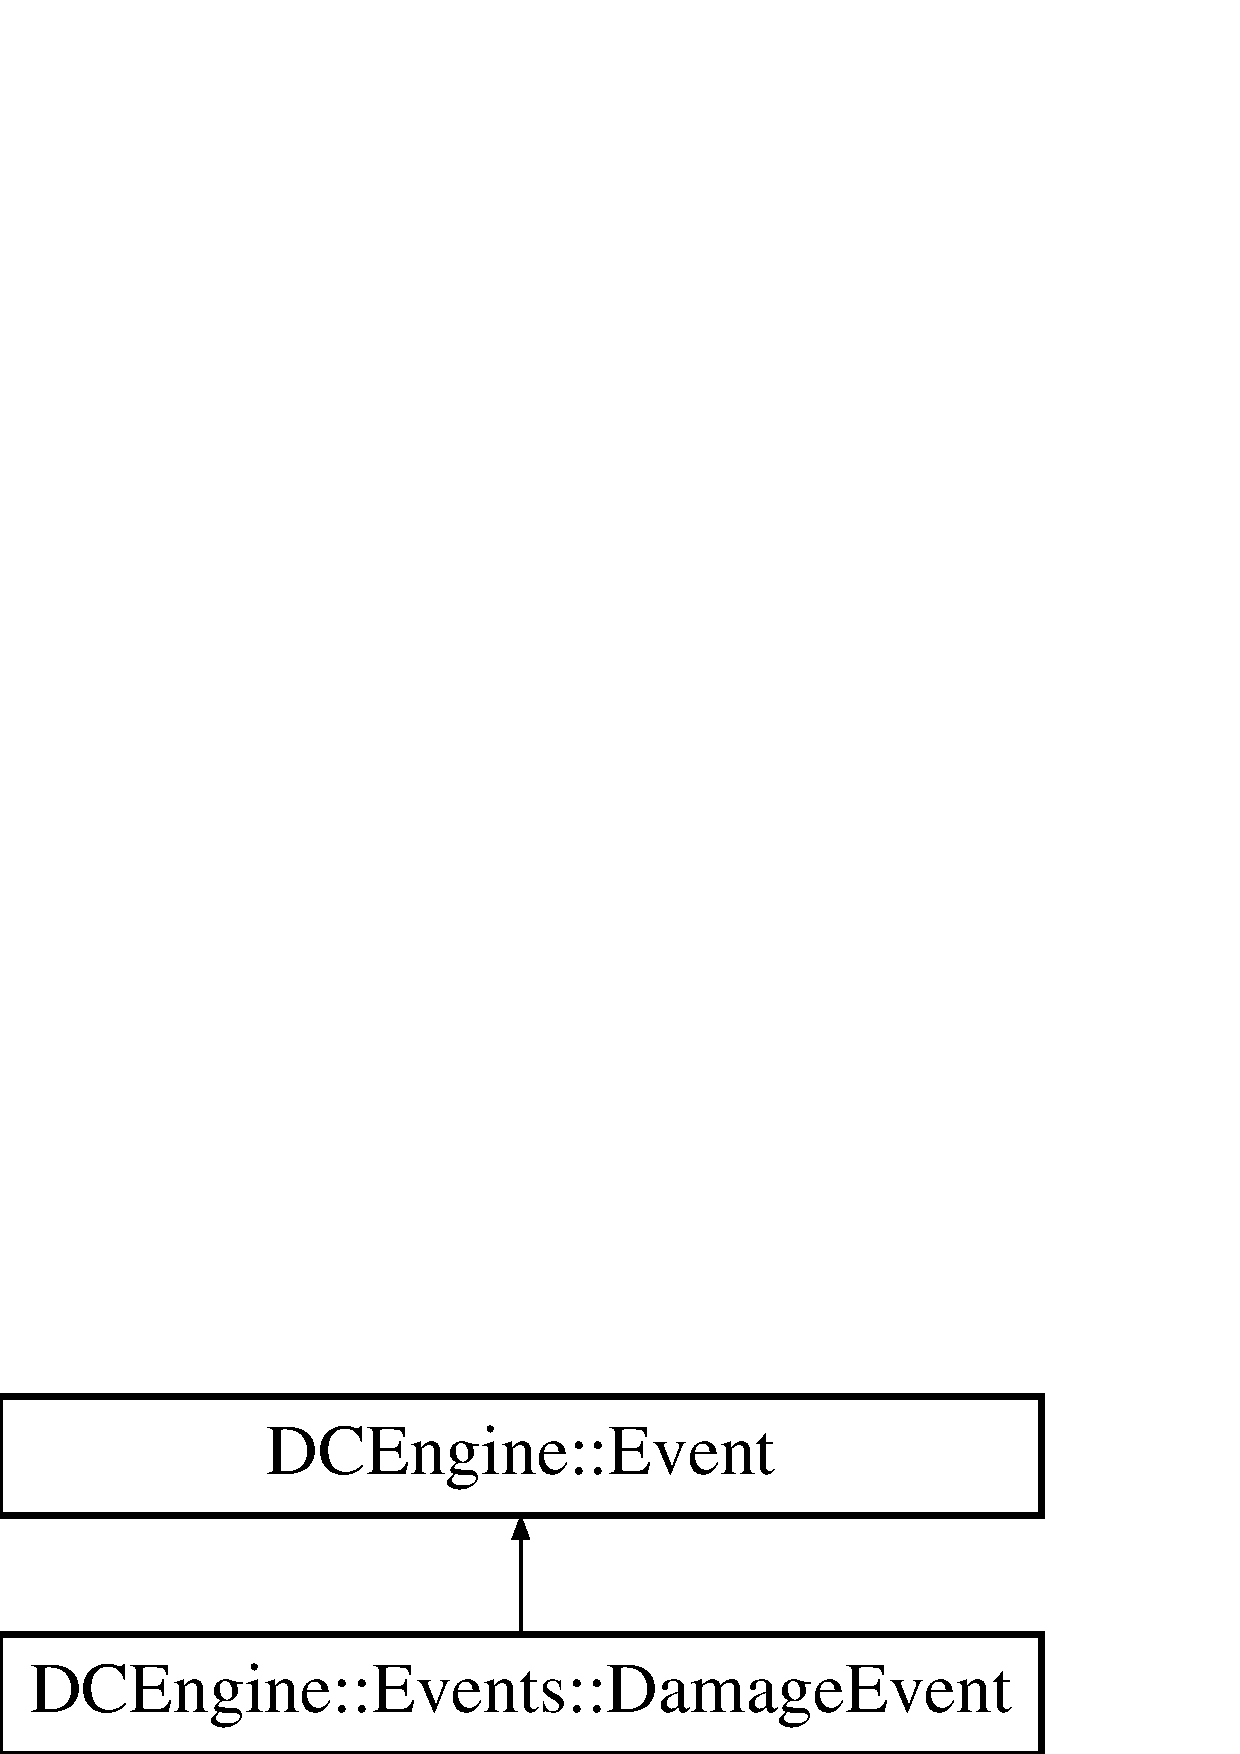
\includegraphics[height=2.000000cm]{classDCEngine_1_1Events_1_1DamageEvent}
\end{center}
\end{figure}
\subsection*{Public Attributes}
\begin{DoxyCompactItemize}
\item 
\hypertarget{classDCEngine_1_1Events_1_1DamageEvent_a2c1741c540fa074b7cc7273e83ab7026}{Real {\bfseries Damage}}\label{classDCEngine_1_1Events_1_1DamageEvent_a2c1741c540fa074b7cc7273e83ab7026}

\end{DoxyCompactItemize}
\subsection*{Additional Inherited Members}


The documentation for this class was generated from the following file\-:\begin{DoxyCompactItemize}
\item 
Projects/\-Rebound/\hyperlink{ReboundEvents_8h}{Rebound\-Events.\-h}\end{DoxyCompactItemize}

\hypertarget{classDCEngine_1_1Components_1_1DebugActions}{\section{D\-C\-Engine\-:\-:Components\-:\-:Debug\-Actions Class Reference}
\label{classDCEngine_1_1Components_1_1DebugActions}\index{D\-C\-Engine\-::\-Components\-::\-Debug\-Actions@{D\-C\-Engine\-::\-Components\-::\-Debug\-Actions}}
}
Inheritance diagram for D\-C\-Engine\-:\-:Components\-:\-:Debug\-Actions\-:\begin{figure}[H]
\begin{center}
\leavevmode
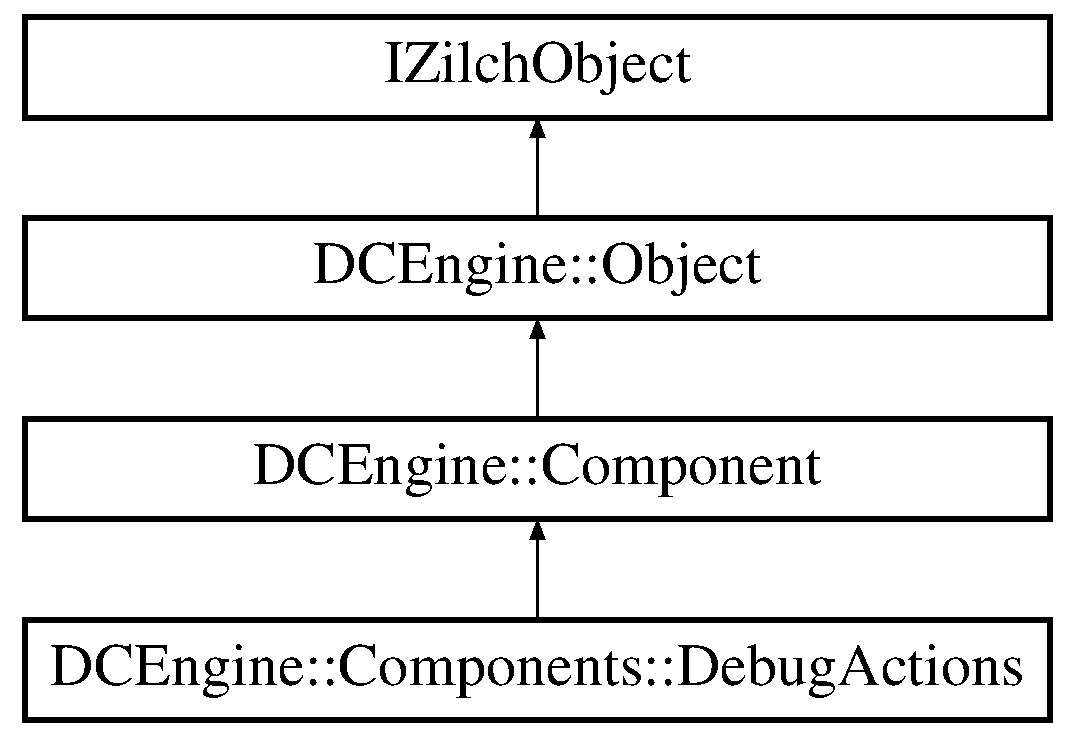
\includegraphics[height=4.000000cm]{classDCEngine_1_1Components_1_1DebugActions}
\end{center}
\end{figure}
\subsection*{Public Member Functions}
\begin{DoxyCompactItemize}
\item 
\hypertarget{classDCEngine_1_1Components_1_1DebugActions_a653959fae2be64469248eaf460e0e7fa}{{\bfseries Zilch\-Declare\-Derived\-Type} (\hyperlink{classDCEngine_1_1Components_1_1DebugActions}{Debug\-Actions}, \hyperlink{classDCEngine_1_1Component}{Component})}\label{classDCEngine_1_1Components_1_1DebugActions_a653959fae2be64469248eaf460e0e7fa}

\item 
\hypertarget{classDCEngine_1_1Components_1_1DebugActions_a8ff6125cb832e96636a897acf684ad56}{{\bfseries Debug\-Actions} (\hyperlink{classDCEngine_1_1Entity}{Entity} \&owner)}\label{classDCEngine_1_1Components_1_1DebugActions_a8ff6125cb832e96636a897acf684ad56}

\item 
\hypertarget{classDCEngine_1_1Components_1_1DebugActions_ac45d922ccffbefd95db11629d21c4330}{void {\bfseries Initialize} ()}\label{classDCEngine_1_1Components_1_1DebugActions_ac45d922ccffbefd95db11629d21c4330}

\item 
\hypertarget{classDCEngine_1_1Components_1_1DebugActions_ab8f50d68c66c465cae5ace796a6cf3c0}{void {\bfseries On\-Key\-Down\-Event} (\hyperlink{classDCEngine_1_1Events_1_1KeyDown}{Events\-::\-Key\-Down} $\ast$event)}\label{classDCEngine_1_1Components_1_1DebugActions_ab8f50d68c66c465cae5ace796a6cf3c0}

\item 
\hypertarget{classDCEngine_1_1Components_1_1DebugActions_aa96500fe6647222d2461c03afdb7f2be}{void {\bfseries On\-Key\-Up\-Event} (\hyperlink{classDCEngine_1_1Events_1_1KeyUp}{Events\-::\-Key\-Up} $\ast$event)}\label{classDCEngine_1_1Components_1_1DebugActions_aa96500fe6647222d2461c03afdb7f2be}

\item 
\hypertarget{classDCEngine_1_1Components_1_1DebugActions_a9fb8c585069602a5d3d599bd60da9c7d}{void {\bfseries On\-Mouse\-Down\-Event} (\hyperlink{classDCEngine_1_1Events_1_1MouseDown}{Events\-::\-Mouse\-Down} $\ast$event)}\label{classDCEngine_1_1Components_1_1DebugActions_a9fb8c585069602a5d3d599bd60da9c7d}

\item 
\hypertarget{classDCEngine_1_1Components_1_1DebugActions_a5ea560c5874ecea5efaf89893a744722}{void {\bfseries On\-Logic\-Update\-Event} (\hyperlink{classDCEngine_1_1Events_1_1LogicUpdate}{Events\-::\-Logic\-Update} $\ast$event)}\label{classDCEngine_1_1Components_1_1DebugActions_a5ea560c5874ecea5efaf89893a744722}

\item 
\hypertarget{classDCEngine_1_1Components_1_1DebugActions_a6e6ae2fd56684a19f5d5c999a8e08c14}{void {\bfseries Test\-Action\-Sequence} ()}\label{classDCEngine_1_1Components_1_1DebugActions_a6e6ae2fd56684a19f5d5c999a8e08c14}

\item 
\hypertarget{classDCEngine_1_1Components_1_1DebugActions_a6c0a2183af7077931fb9e9e8883cf2c0}{void {\bfseries Test\-Ray\-Casting} ()}\label{classDCEngine_1_1Components_1_1DebugActions_a6c0a2183af7077931fb9e9e8883cf2c0}

\item 
\hypertarget{classDCEngine_1_1Components_1_1DebugActions_a3abfc0f7d9b76ac363b31f74e106892a}{void {\bfseries Debug\-Draw} ()}\label{classDCEngine_1_1Components_1_1DebugActions_a3abfc0f7d9b76ac363b31f74e106892a}

\end{DoxyCompactItemize}
\subsection*{Additional Inherited Members}


The documentation for this class was generated from the following files\-:\begin{DoxyCompactItemize}
\item 
Core/\-Components/\hyperlink{DebugActions_8h}{Debug\-Actions.\-h}\item 
Core/\-Components/\hyperlink{DebugActions_8cpp}{Debug\-Actions.\-cpp}\end{DoxyCompactItemize}

\hypertarget{classDCEngine_1_1Components_1_1DebugAudio}{\section{D\-C\-Engine\-:\-:Components\-:\-:Debug\-Audio Class Reference}
\label{classDCEngine_1_1Components_1_1DebugAudio}\index{D\-C\-Engine\-::\-Components\-::\-Debug\-Audio@{D\-C\-Engine\-::\-Components\-::\-Debug\-Audio}}
}
Inheritance diagram for D\-C\-Engine\-:\-:Components\-:\-:Debug\-Audio\-:\begin{figure}[H]
\begin{center}
\leavevmode
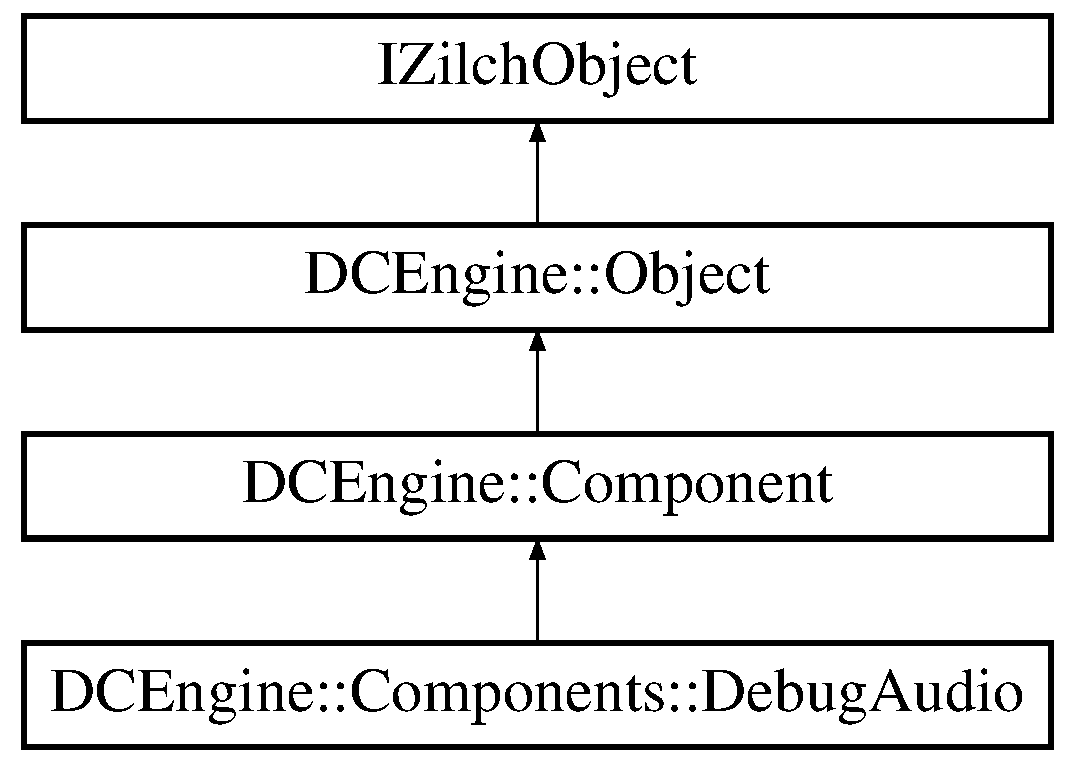
\includegraphics[height=4.000000cm]{classDCEngine_1_1Components_1_1DebugAudio}
\end{center}
\end{figure}
\subsection*{Public Member Functions}
\begin{DoxyCompactItemize}
\item 
\hypertarget{classDCEngine_1_1Components_1_1DebugAudio_acd62559a4fe42b591f51e10a5f65fb55}{{\bfseries Debug\-Audio} (\hyperlink{classDCEngine_1_1Entity}{Entity} \&owner)}\label{classDCEngine_1_1Components_1_1DebugAudio_acd62559a4fe42b591f51e10a5f65fb55}

\item 
\hypertarget{classDCEngine_1_1Components_1_1DebugAudio_ae6c4b191bd9918bcf21fabb4eda1aa01}{void {\bfseries Initialize} ()}\label{classDCEngine_1_1Components_1_1DebugAudio_ae6c4b191bd9918bcf21fabb4eda1aa01}

\item 
\hypertarget{classDCEngine_1_1Components_1_1DebugAudio_a9523b0bddda77ff319a8095dbc3e5388}{virtual void {\bfseries Serialize} (Json\-::\-Value \&root)}\label{classDCEngine_1_1Components_1_1DebugAudio_a9523b0bddda77ff319a8095dbc3e5388}

\item 
\hypertarget{classDCEngine_1_1Components_1_1DebugAudio_a3d3d071d538ea58e809f0a90fa4ee462}{virtual void {\bfseries Deserialize} (Json\-::\-Value \&root)}\label{classDCEngine_1_1Components_1_1DebugAudio_a3d3d071d538ea58e809f0a90fa4ee462}

\item 
\hypertarget{classDCEngine_1_1Components_1_1DebugAudio_a27c68decdddba9f7cbc76c94046239b2}{void {\bfseries On\-Key\-Down\-Event} (\hyperlink{classDCEngine_1_1Events_1_1KeyDown}{Events\-::\-Key\-Down} $\ast$event)}\label{classDCEngine_1_1Components_1_1DebugAudio_a27c68decdddba9f7cbc76c94046239b2}

\item 
\hypertarget{classDCEngine_1_1Components_1_1DebugAudio_a0bcb6354208a3e2753a1f6057adfcdbd}{void {\bfseries On\-Key\-Up\-Event} (\hyperlink{classDCEngine_1_1Events_1_1KeyUp}{Events\-::\-Key\-Up} $\ast$event)}\label{classDCEngine_1_1Components_1_1DebugAudio_a0bcb6354208a3e2753a1f6057adfcdbd}

\item 
void \hyperlink{classDCEngine_1_1Components_1_1DebugAudio_a4d3332809c4607dea35a5f98e2ce4fb0}{Change\-Track} (std\-::string \&track)
\begin{DoxyCompactList}\small\item\em Changes the currently playing track. \end{DoxyCompactList}\end{DoxyCompactItemize}
\subsection*{Public Attributes}
\begin{DoxyCompactItemize}
\item 
\hypertarget{classDCEngine_1_1Components_1_1DebugAudio_ae66e77d01d3937a9572560d24c7dcb0a}{String {\bfseries Track1} = \char`\"{}soulja\char`\"{}}\label{classDCEngine_1_1Components_1_1DebugAudio_ae66e77d01d3937a9572560d24c7dcb0a}

\item 
\hypertarget{classDCEngine_1_1Components_1_1DebugAudio_aeddb7b199357f65927c2b1fa89f9469e}{String {\bfseries Track2}}\label{classDCEngine_1_1Components_1_1DebugAudio_aeddb7b199357f65927c2b1fa89f9469e}

\item 
\hypertarget{classDCEngine_1_1Components_1_1DebugAudio_a89192dbb7c84dc3c2703c3c1d362fc8d}{String {\bfseries Track3}}\label{classDCEngine_1_1Components_1_1DebugAudio_a89192dbb7c84dc3c2703c3c1d362fc8d}

\item 
\hypertarget{classDCEngine_1_1Components_1_1DebugAudio_adeaa1d45f4cdb632ab0ce459734f7232}{String {\bfseries Current\-Sound\-Cue}}\label{classDCEngine_1_1Components_1_1DebugAudio_adeaa1d45f4cdb632ab0ce459734f7232}

\end{DoxyCompactItemize}
\subsection*{Additional Inherited Members}


\subsection{Member Function Documentation}
\hypertarget{classDCEngine_1_1Components_1_1DebugAudio_a4d3332809c4607dea35a5f98e2ce4fb0}{\index{D\-C\-Engine\-::\-Components\-::\-Debug\-Audio@{D\-C\-Engine\-::\-Components\-::\-Debug\-Audio}!Change\-Track@{Change\-Track}}
\index{Change\-Track@{Change\-Track}!DCEngine::Components::DebugAudio@{D\-C\-Engine\-::\-Components\-::\-Debug\-Audio}}
\subsubsection[{Change\-Track}]{\setlength{\rightskip}{0pt plus 5cm}void D\-C\-Engine\-::\-Components\-::\-Debug\-Audio\-::\-Change\-Track (
\begin{DoxyParamCaption}
\item[{std\-::string \&}]{track}
\end{DoxyParamCaption}
)}}\label{classDCEngine_1_1Components_1_1DebugAudio_a4d3332809c4607dea35a5f98e2ce4fb0}


Changes the currently playing track. 

\begin{DoxyNote}{Note}
\hyperlink{classThe}{The} name of the track (sound file) to play. 
\end{DoxyNote}


The documentation for this class was generated from the following files\-:\begin{DoxyCompactItemize}
\item 
Core/\-Components/\hyperlink{DebugAudio_8h}{Debug\-Audio.\-h}\item 
Core/\-Components/\hyperlink{DebugAudio_8cpp}{Debug\-Audio.\-cpp}\end{DoxyCompactItemize}

\hypertarget{classDCEngine_1_1Components_1_1DebugCamera}{\section{D\-C\-Engine\-:\-:Components\-:\-:Debug\-Camera Class Reference}
\label{classDCEngine_1_1Components_1_1DebugCamera}\index{D\-C\-Engine\-::\-Components\-::\-Debug\-Camera@{D\-C\-Engine\-::\-Components\-::\-Debug\-Camera}}
}
Inheritance diagram for D\-C\-Engine\-:\-:Components\-:\-:Debug\-Camera\-:\begin{figure}[H]
\begin{center}
\leavevmode
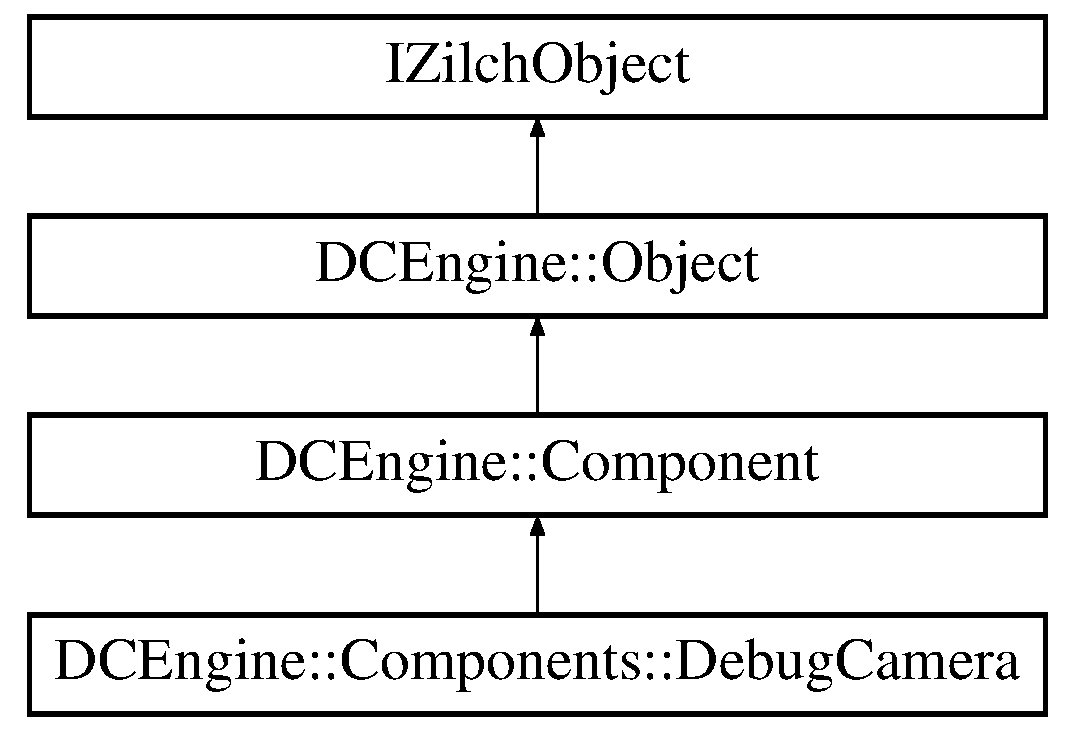
\includegraphics[height=4.000000cm]{classDCEngine_1_1Components_1_1DebugCamera}
\end{center}
\end{figure}
\subsection*{Public Member Functions}
\begin{DoxyCompactItemize}
\item 
\hypertarget{classDCEngine_1_1Components_1_1DebugCamera_a7aba3c7de5f17f4633fd39c5866228b7}{{\bfseries Debug\-Camera} (\hyperlink{classDCEngine_1_1Entity}{Entity} \&owner)}\label{classDCEngine_1_1Components_1_1DebugCamera_a7aba3c7de5f17f4633fd39c5866228b7}

\item 
\hypertarget{classDCEngine_1_1Components_1_1DebugCamera_a993bc1ebff7b239dc056767f77f05b0f}{void {\bfseries Initialize} ()}\label{classDCEngine_1_1Components_1_1DebugCamera_a993bc1ebff7b239dc056767f77f05b0f}

\item 
\hypertarget{classDCEngine_1_1Components_1_1DebugCamera_a1eec4e7cd651522d4bbb9058c3ceaf76}{void {\bfseries On\-Key\-Down\-Event} (\hyperlink{classDCEngine_1_1Events_1_1KeyDown}{Events\-::\-Key\-Down} $\ast$event)}\label{classDCEngine_1_1Components_1_1DebugCamera_a1eec4e7cd651522d4bbb9058c3ceaf76}

\item 
\hypertarget{classDCEngine_1_1Components_1_1DebugCamera_ac26e2cb348c00207bef401d0c2105e88}{void {\bfseries On\-Key\-Up\-Event} (\hyperlink{classDCEngine_1_1Events_1_1KeyUp}{Events\-::\-Key\-Up} $\ast$event)}\label{classDCEngine_1_1Components_1_1DebugCamera_ac26e2cb348c00207bef401d0c2105e88}

\item 
\hypertarget{classDCEngine_1_1Components_1_1DebugCamera_a5fe8a650881c6ac60fe50667f67899fb}{void {\bfseries Print\-Translation} ()}\label{classDCEngine_1_1Components_1_1DebugCamera_a5fe8a650881c6ac60fe50667f67899fb}

\end{DoxyCompactItemize}
\subsection*{Public Attributes}
\begin{DoxyCompactItemize}
\item 
\hypertarget{classDCEngine_1_1Components_1_1DebugCamera_ae569e466b9733d7f6fbdd77f40a82a0e}{Real {\bfseries Move\-Speed} = 3}\label{classDCEngine_1_1Components_1_1DebugCamera_ae569e466b9733d7f6fbdd77f40a82a0e}

\item 
\hypertarget{classDCEngine_1_1Components_1_1DebugCamera_a53a1bf819df296c48ad5f078403b9198}{Real {\bfseries Rot\-Speed} = 15}\label{classDCEngine_1_1Components_1_1DebugCamera_a53a1bf819df296c48ad5f078403b9198}

\item 
\hypertarget{classDCEngine_1_1Components_1_1DebugCamera_ac336fdc9b934ef4057d73199f6720442}{Real {\bfseries Zoom\-Speed} = 10}\label{classDCEngine_1_1Components_1_1DebugCamera_ac336fdc9b934ef4057d73199f6720442}

\end{DoxyCompactItemize}
\subsection*{Additional Inherited Members}


The documentation for this class was generated from the following files\-:\begin{DoxyCompactItemize}
\item 
Core/\-Components/\hyperlink{DebugCamera_8h}{Debug\-Camera.\-h}\item 
Core/\-Components/\hyperlink{DebugCamera_8cpp}{Debug\-Camera.\-cpp}\end{DoxyCompactItemize}

\hypertarget{classDCEngine_1_1Components_1_1DebugCollider}{\section{D\-C\-Engine\-:\-:Components\-:\-:Debug\-Collider Class Reference}
\label{classDCEngine_1_1Components_1_1DebugCollider}\index{D\-C\-Engine\-::\-Components\-::\-Debug\-Collider@{D\-C\-Engine\-::\-Components\-::\-Debug\-Collider}}
}
Inheritance diagram for D\-C\-Engine\-:\-:Components\-:\-:Debug\-Collider\-:\begin{figure}[H]
\begin{center}
\leavevmode
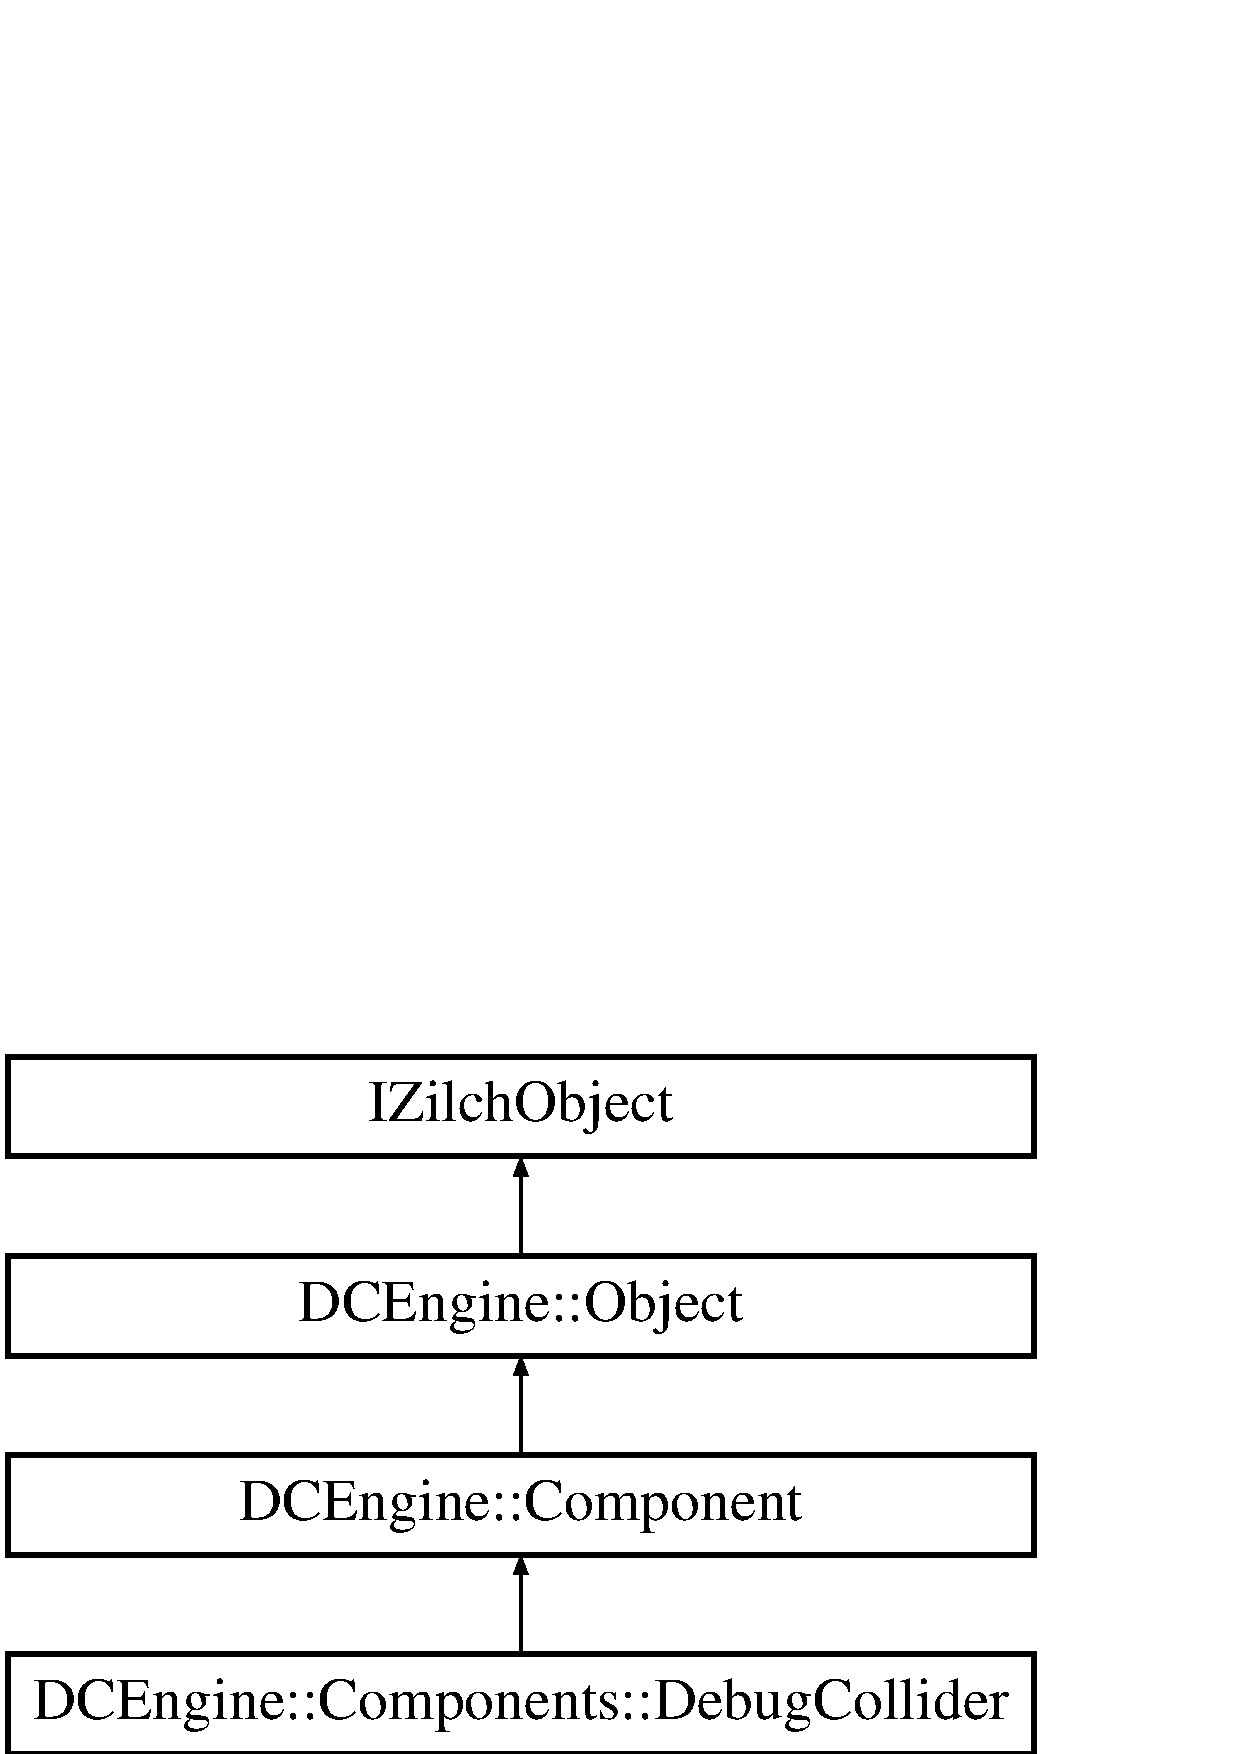
\includegraphics[height=4.000000cm]{classDCEngine_1_1Components_1_1DebugCollider}
\end{center}
\end{figure}
\subsection*{Public Member Functions}
\begin{DoxyCompactItemize}
\item 
\hypertarget{classDCEngine_1_1Components_1_1DebugCollider_a40dec5fc957f92340508b3570e513874}{{\bfseries Debug\-Collider} (\hyperlink{classDCEngine_1_1Entity}{Entity} \&owner)}\label{classDCEngine_1_1Components_1_1DebugCollider_a40dec5fc957f92340508b3570e513874}

\item 
\hypertarget{classDCEngine_1_1Components_1_1DebugCollider_ae752ba4d3b7dc2f8857536b277c9b2a2}{void {\bfseries Initialize} ()}\label{classDCEngine_1_1Components_1_1DebugCollider_ae752ba4d3b7dc2f8857536b277c9b2a2}

\item 
\hypertarget{classDCEngine_1_1Components_1_1DebugCollider_a0f5a33e7a1012393e58073505e47fdb4}{virtual void {\bfseries Serialize} (Json\-::\-Value \&root)}\label{classDCEngine_1_1Components_1_1DebugCollider_a0f5a33e7a1012393e58073505e47fdb4}

\item 
\hypertarget{classDCEngine_1_1Components_1_1DebugCollider_a6cb73edd53aa5fb98841aecf4f7f3b61}{virtual void {\bfseries Deserialize} (Json\-::\-Value \&root)}\label{classDCEngine_1_1Components_1_1DebugCollider_a6cb73edd53aa5fb98841aecf4f7f3b61}

\item 
\hypertarget{classDCEngine_1_1Components_1_1DebugCollider_af31ccceeac52e79a796fdb594336bd58}{void {\bfseries On\-Collision\-Started\-Event} (\hyperlink{classDCEngine_1_1Events_1_1CollisionStarted}{Events\-::\-Collision\-Started} $\ast$event)}\label{classDCEngine_1_1Components_1_1DebugCollider_af31ccceeac52e79a796fdb594336bd58}

\item 
\hypertarget{classDCEngine_1_1Components_1_1DebugCollider_acc41c399395c2241836bfa3d66e72e59}{void {\bfseries On\-Collision\-Ended\-Event} (\hyperlink{classDCEngine_1_1Events_1_1CollisionEnded}{Events\-::\-Collision\-Ended} $\ast$event)}\label{classDCEngine_1_1Components_1_1DebugCollider_acc41c399395c2241836bfa3d66e72e59}

\end{DoxyCompactItemize}
\subsection*{Public Attributes}
\begin{DoxyCompactItemize}
\item 
\hypertarget{classDCEngine_1_1Components_1_1DebugCollider_aa969737c20be282bb1dbfd2708ec061f}{Boolean {\bfseries Change\-Color\-On\-Collide} = false}\label{classDCEngine_1_1Components_1_1DebugCollider_aa969737c20be282bb1dbfd2708ec061f}

\item 
\hypertarget{classDCEngine_1_1Components_1_1DebugCollider_a576f44de845231d16221b72b274531f2}{Vec4 {\bfseries Collision\-Color} = Vec4(1, 0, 0, 1)}\label{classDCEngine_1_1Components_1_1DebugCollider_a576f44de845231d16221b72b274531f2}

\item 
\hypertarget{classDCEngine_1_1Components_1_1DebugCollider_a7c44cbb7084971b859aaa1563b9b9070}{Vec4 {\bfseries Sprite\-Color}}\label{classDCEngine_1_1Components_1_1DebugCollider_a7c44cbb7084971b859aaa1563b9b9070}

\end{DoxyCompactItemize}
\subsection*{Additional Inherited Members}


The documentation for this class was generated from the following files\-:\begin{DoxyCompactItemize}
\item 
Core/\-Components/\hyperlink{DebugCollider_8h}{Debug\-Collider.\-h}\item 
Core/\-Components/\hyperlink{DebugCollider_8cpp}{Debug\-Collider.\-cpp}\end{DoxyCompactItemize}

\hypertarget{classDCEngine_1_1DebugDrawObject}{\section{D\-C\-Engine\-:\-:Debug\-Draw\-Object Class Reference}
\label{classDCEngine_1_1DebugDrawObject}\index{D\-C\-Engine\-::\-Debug\-Draw\-Object@{D\-C\-Engine\-::\-Debug\-Draw\-Object}}
}
Inheritance diagram for D\-C\-Engine\-:\-:Debug\-Draw\-Object\-:\begin{figure}[H]
\begin{center}
\leavevmode
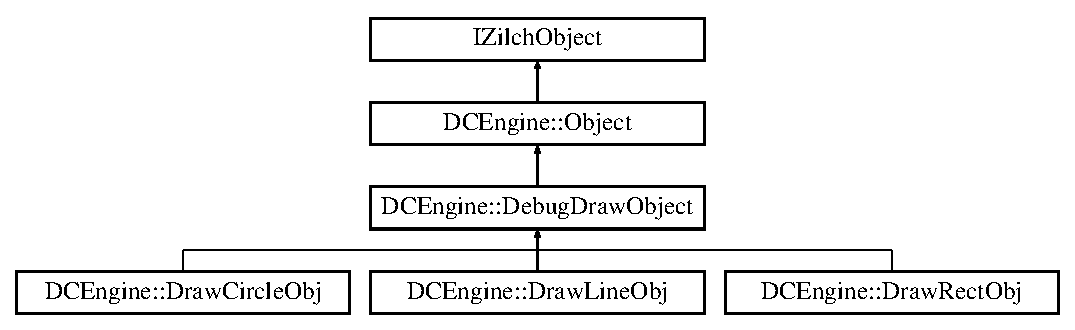
\includegraphics[height=3.992870cm]{classDCEngine_1_1DebugDrawObject}
\end{center}
\end{figure}
\subsection*{Public Member Functions}
\begin{DoxyCompactItemize}
\item 
\hypertarget{classDCEngine_1_1DebugDrawObject_a7d80a0a2d5ea0e723f7a5df0cf4c7f04}{virtual void {\bfseries Draw} ()}\label{classDCEngine_1_1DebugDrawObject_a7d80a0a2d5ea0e723f7a5df0cf4c7f04}

\end{DoxyCompactItemize}
\subsection*{Additional Inherited Members}


The documentation for this class was generated from the following file\-:\begin{DoxyCompactItemize}
\item 
Core/\-Objects/\hyperlink{DebugDraw_8h}{Debug\-Draw.\-h}\end{DoxyCompactItemize}

\hypertarget{classDCEngine_1_1Components_1_1DebugFade}{\section{D\-C\-Engine\-:\-:Components\-:\-:Debug\-Fade Class Reference}
\label{classDCEngine_1_1Components_1_1DebugFade}\index{D\-C\-Engine\-::\-Components\-::\-Debug\-Fade@{D\-C\-Engine\-::\-Components\-::\-Debug\-Fade}}
}
Inheritance diagram for D\-C\-Engine\-:\-:Components\-:\-:Debug\-Fade\-:\begin{figure}[H]
\begin{center}
\leavevmode
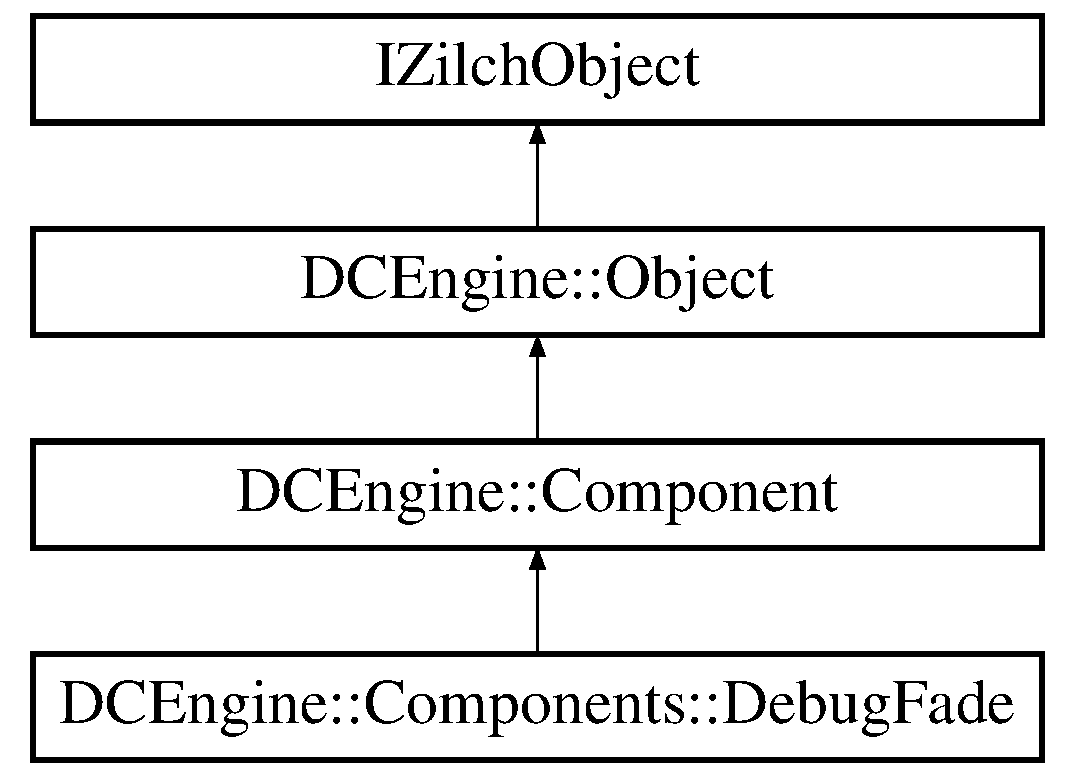
\includegraphics[height=4.000000cm]{classDCEngine_1_1Components_1_1DebugFade}
\end{center}
\end{figure}
\subsection*{Public Member Functions}
\begin{DoxyCompactItemize}
\item 
\hypertarget{classDCEngine_1_1Components_1_1DebugFade_a8625c037a508aa8de8e27bca9d385c1b}{{\bfseries Debug\-Fade} (\hyperlink{classDCEngine_1_1Entity}{Entity} \&owner)}\label{classDCEngine_1_1Components_1_1DebugFade_a8625c037a508aa8de8e27bca9d385c1b}

\item 
\hypertarget{classDCEngine_1_1Components_1_1DebugFade_aecadf44587b7b8549730cdc1bfc3fb6a}{void {\bfseries Initialize} ()}\label{classDCEngine_1_1Components_1_1DebugFade_aecadf44587b7b8549730cdc1bfc3fb6a}

\item 
\hypertarget{classDCEngine_1_1Components_1_1DebugFade_aadb50885d12440dea7e908c6390d0c50}{virtual void {\bfseries Serialize} (Json\-::\-Value \&root)}\label{classDCEngine_1_1Components_1_1DebugFade_aadb50885d12440dea7e908c6390d0c50}

\item 
\hypertarget{classDCEngine_1_1Components_1_1DebugFade_af77bd31f6c310e3ad69a8068847a76b0}{virtual void {\bfseries Deserialize} (Json\-::\-Value \&root)}\label{classDCEngine_1_1Components_1_1DebugFade_af77bd31f6c310e3ad69a8068847a76b0}

\item 
\hypertarget{classDCEngine_1_1Components_1_1DebugFade_a675c986f820f09e75c732b15752ed1c1}{void {\bfseries On\-Logic\-Update\-Event} (\hyperlink{classDCEngine_1_1Events_1_1LogicUpdate}{Events\-::\-Logic\-Update} $\ast$event)}\label{classDCEngine_1_1Components_1_1DebugFade_a675c986f820f09e75c732b15752ed1c1}

\end{DoxyCompactItemize}
\subsection*{Public Attributes}
\begin{DoxyCompactItemize}
\item 
\hypertarget{classDCEngine_1_1Components_1_1DebugFade_a406c11e704485cc641cabc290749abdc}{\hyperlink{classDCEngine_1_1Components_1_1Sprite}{Sprite} $\ast$ {\bfseries Sprite\-Component}}\label{classDCEngine_1_1Components_1_1DebugFade_a406c11e704485cc641cabc290749abdc}

\item 
\hypertarget{classDCEngine_1_1Components_1_1DebugFade_a34b8ef12d8f7919826f3eb94e2bfdbec}{Real {\bfseries Fade\-Out\-Dur} = 10}\label{classDCEngine_1_1Components_1_1DebugFade_a34b8ef12d8f7919826f3eb94e2bfdbec}

\item 
\hypertarget{classDCEngine_1_1Components_1_1DebugFade_a9fcd4d4126eb6198f32d34a87c238c50}{Vec4 {\bfseries Fade\-Color} = Vec4(0, 0, 0, 0)}\label{classDCEngine_1_1Components_1_1DebugFade_a9fcd4d4126eb6198f32d34a87c238c50}

\end{DoxyCompactItemize}
\subsection*{Additional Inherited Members}


The documentation for this class was generated from the following files\-:\begin{DoxyCompactItemize}
\item 
Core/\-Components/Debug\-Fade.\-h\item 
Core/\-Components/\hyperlink{DebugFade_8cpp}{Debug\-Fade.\-cpp}\end{DoxyCompactItemize}

\hypertarget{classDCEngine_1_1Components_1_1DebugMoveController}{\section{D\-C\-Engine\-:\-:Components\-:\-:Debug\-Move\-Controller Class Reference}
\label{classDCEngine_1_1Components_1_1DebugMoveController}\index{D\-C\-Engine\-::\-Components\-::\-Debug\-Move\-Controller@{D\-C\-Engine\-::\-Components\-::\-Debug\-Move\-Controller}}
}
Inheritance diagram for D\-C\-Engine\-:\-:Components\-:\-:Debug\-Move\-Controller\-:\begin{figure}[H]
\begin{center}
\leavevmode
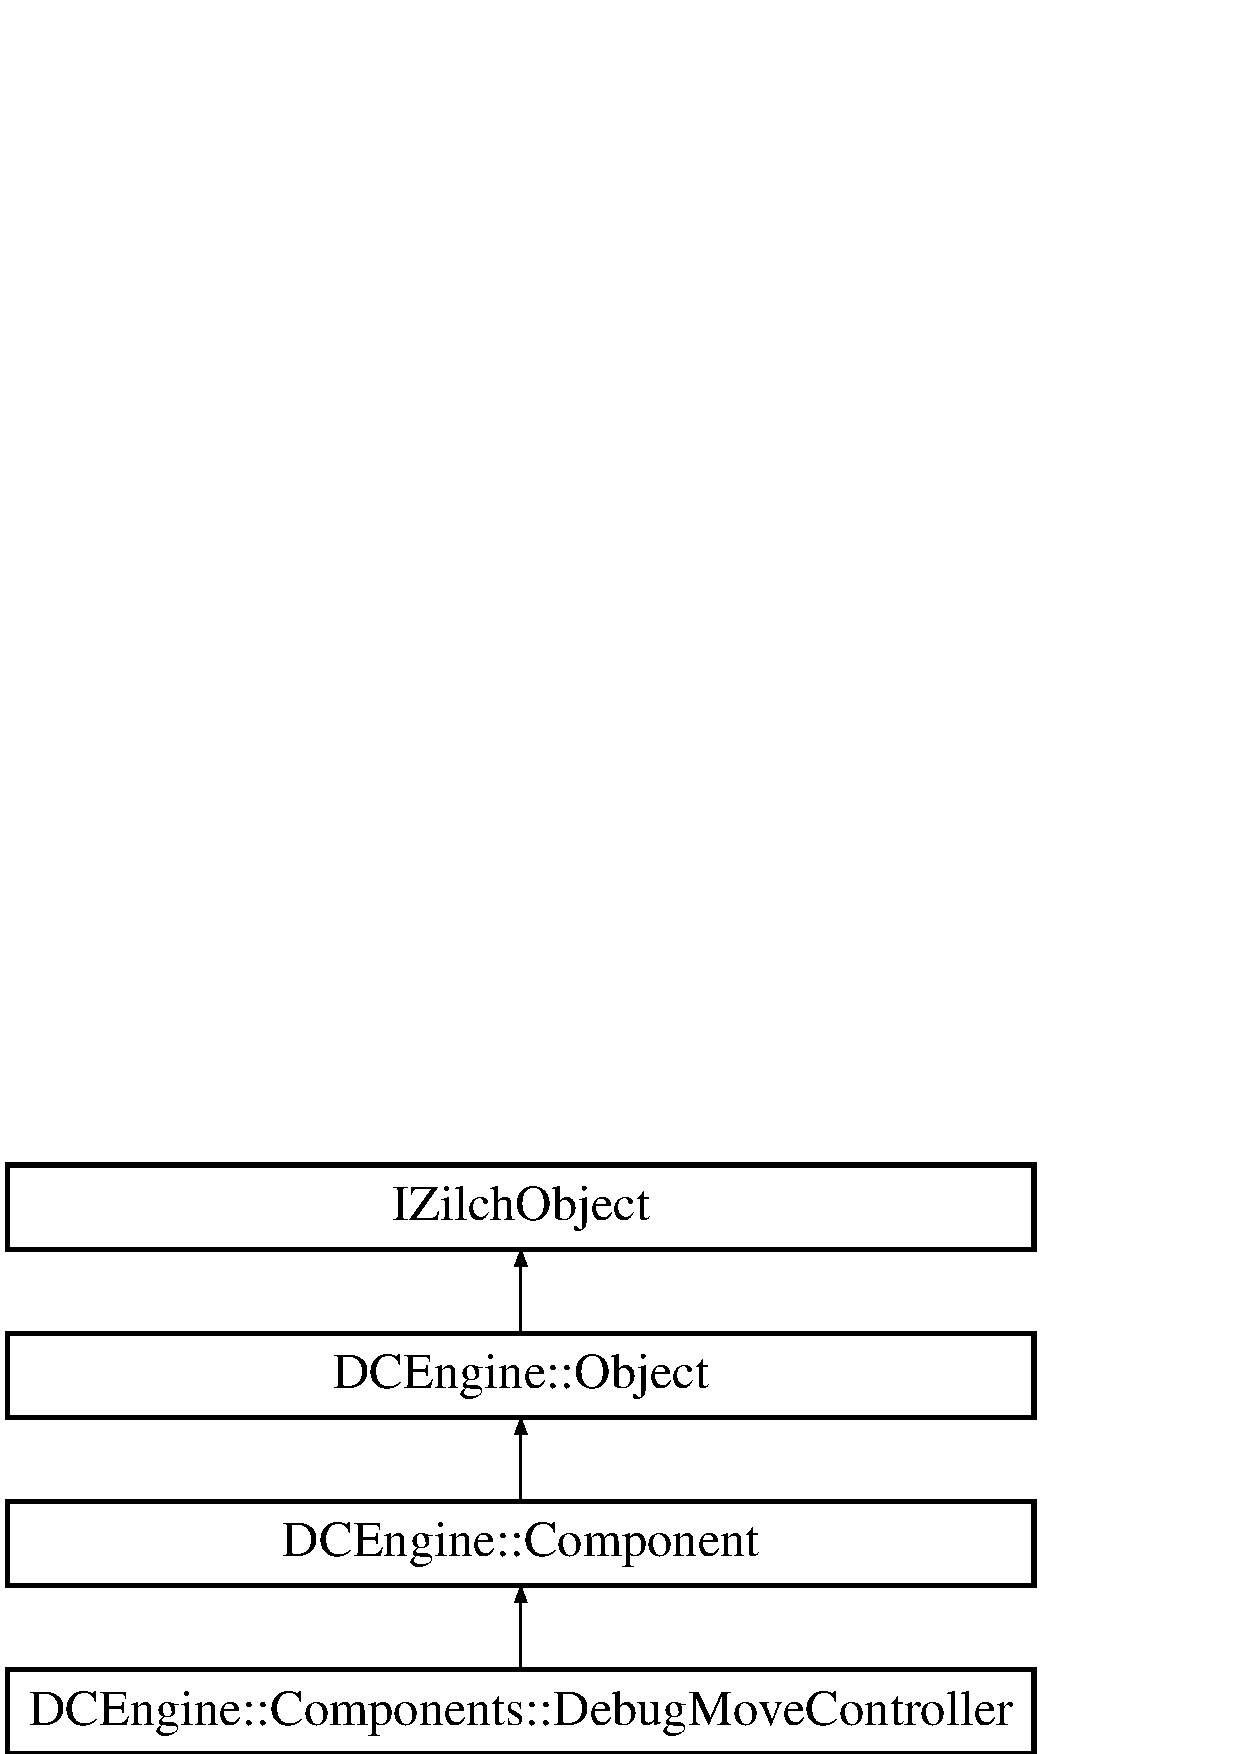
\includegraphics[height=4.000000cm]{classDCEngine_1_1Components_1_1DebugMoveController}
\end{center}
\end{figure}
\subsection*{Public Member Functions}
\begin{DoxyCompactItemize}
\item 
\hypertarget{classDCEngine_1_1Components_1_1DebugMoveController_a217c79bcbaeed75937147005f7c2bf59}{{\bfseries Debug\-Move\-Controller} (\hyperlink{classDCEngine_1_1Entity}{Entity} \&owner)}\label{classDCEngine_1_1Components_1_1DebugMoveController_a217c79bcbaeed75937147005f7c2bf59}

\item 
\hypertarget{classDCEngine_1_1Components_1_1DebugMoveController_a978031840990e725c700e9f3c6f11eb2}{void {\bfseries Initialize} ()}\label{classDCEngine_1_1Components_1_1DebugMoveController_a978031840990e725c700e9f3c6f11eb2}

\item 
\hypertarget{classDCEngine_1_1Components_1_1DebugMoveController_aeb04743b0ae70944edaed68336be121b}{virtual void {\bfseries Serialize} (Json\-::\-Value \&root)}\label{classDCEngine_1_1Components_1_1DebugMoveController_aeb04743b0ae70944edaed68336be121b}

\item 
\hypertarget{classDCEngine_1_1Components_1_1DebugMoveController_a1f4f2e805cc5ed4a22bbefd7e67b4ef4}{virtual void {\bfseries Deserialize} (Json\-::\-Value \&root)}\label{classDCEngine_1_1Components_1_1DebugMoveController_a1f4f2e805cc5ed4a22bbefd7e67b4ef4}

\item 
\hypertarget{classDCEngine_1_1Components_1_1DebugMoveController_aa74473e1cdb4378132995b8a603e01cd}{void {\bfseries On\-Key\-Down\-Event} (\hyperlink{classDCEngine_1_1Events_1_1KeyDown}{Events\-::\-Key\-Down} $\ast$event)}\label{classDCEngine_1_1Components_1_1DebugMoveController_aa74473e1cdb4378132995b8a603e01cd}

\item 
\hypertarget{classDCEngine_1_1Components_1_1DebugMoveController_a9287cd69e7501d4b7f7e47f70dbcf112}{void {\bfseries On\-Key\-Up\-Event} (\hyperlink{classDCEngine_1_1Events_1_1KeyUp}{Events\-::\-Key\-Up} $\ast$event)}\label{classDCEngine_1_1Components_1_1DebugMoveController_a9287cd69e7501d4b7f7e47f70dbcf112}

\item 
\hypertarget{classDCEngine_1_1Components_1_1DebugMoveController_a9938d06043a6faf0c6936653a253818c}{void {\bfseries On\-Mouse\-Down\-Event} (\hyperlink{classDCEngine_1_1Events_1_1MouseDown}{Events\-::\-Mouse\-Down} $\ast$event)}\label{classDCEngine_1_1Components_1_1DebugMoveController_a9938d06043a6faf0c6936653a253818c}

\item 
\hypertarget{classDCEngine_1_1Components_1_1DebugMoveController_a27928e27655218bff759d9957e4c5957}{void {\bfseries On\-Logic\-Update\-Event} (\hyperlink{classDCEngine_1_1Events_1_1LogicUpdate}{Events\-::\-Logic\-Update} $\ast$event)}\label{classDCEngine_1_1Components_1_1DebugMoveController_a27928e27655218bff759d9957e4c5957}

\item 
\hypertarget{classDCEngine_1_1Components_1_1DebugMoveController_a7e9d52bec89aaf3bfbfa488410bc342f}{void {\bfseries Set\-Footstep\-Sound} (std\-::string \&soundfile\-Name)}\label{classDCEngine_1_1Components_1_1DebugMoveController_a7e9d52bec89aaf3bfbfa488410bc342f}

\end{DoxyCompactItemize}
\subsection*{Public Attributes}
\begin{DoxyCompactItemize}
\item 
\hypertarget{classDCEngine_1_1Components_1_1DebugMoveController_a88988103f12f82e91aa791f608b91a00}{bool {\bfseries Translation} = false}\label{classDCEngine_1_1Components_1_1DebugMoveController_a88988103f12f82e91aa791f608b91a00}

\item 
\hypertarget{classDCEngine_1_1Components_1_1DebugMoveController_a2864d2a5f695154f534477a14b555071}{Real {\bfseries Move\-Speed} = 10}\label{classDCEngine_1_1Components_1_1DebugMoveController_a2864d2a5f695154f534477a14b555071}

\item 
\hypertarget{classDCEngine_1_1Components_1_1DebugMoveController_a2a95e0c57a4fd8a2b44297ef01244fe7}{Real {\bfseries Rot\-Speed} = 15}\label{classDCEngine_1_1Components_1_1DebugMoveController_a2a95e0c57a4fd8a2b44297ef01244fe7}

\item 
\hypertarget{classDCEngine_1_1Components_1_1DebugMoveController_a018c3509fca8f6c545976e6c354086bb}{Real {\bfseries Jump\-Multiplier} = 5}\label{classDCEngine_1_1Components_1_1DebugMoveController_a018c3509fca8f6c545976e6c354086bb}

\item 
\hypertarget{classDCEngine_1_1Components_1_1DebugMoveController_a893c0ee9fc1fff7c68e61521516e4240}{\hyperlink{classDCEngine_1_1Components_1_1Transform}{Transform} $\ast$ {\bfseries Transform\-Ref}}\label{classDCEngine_1_1Components_1_1DebugMoveController_a893c0ee9fc1fff7c68e61521516e4240}

\item 
\hypertarget{classDCEngine_1_1Components_1_1DebugMoveController_a4b8a59951be8e7e3778d835949c9c1da}{\hyperlink{classDCEngine_1_1Components_1_1RigidBody}{Rigid\-Body} $\ast$ {\bfseries Rigid\-Body\-Ref}}\label{classDCEngine_1_1Components_1_1DebugMoveController_a4b8a59951be8e7e3778d835949c9c1da}

\end{DoxyCompactItemize}
\subsection*{Additional Inherited Members}


The documentation for this class was generated from the following files\-:\begin{DoxyCompactItemize}
\item 
Core/\-Components/\hyperlink{DebugMoveController_8h}{Debug\-Move\-Controller.\-h}\item 
Core/\-Components/Debug\-Move\-Controller.\-cpp\end{DoxyCompactItemize}

\hypertarget{classDCEngine_1_1Components_1_1DebugReport}{\section{D\-C\-Engine\-:\-:Components\-:\-:Debug\-Report Class Reference}
\label{classDCEngine_1_1Components_1_1DebugReport}\index{D\-C\-Engine\-::\-Components\-::\-Debug\-Report@{D\-C\-Engine\-::\-Components\-::\-Debug\-Report}}
}
Inheritance diagram for D\-C\-Engine\-:\-:Components\-:\-:Debug\-Report\-:\begin{figure}[H]
\begin{center}
\leavevmode
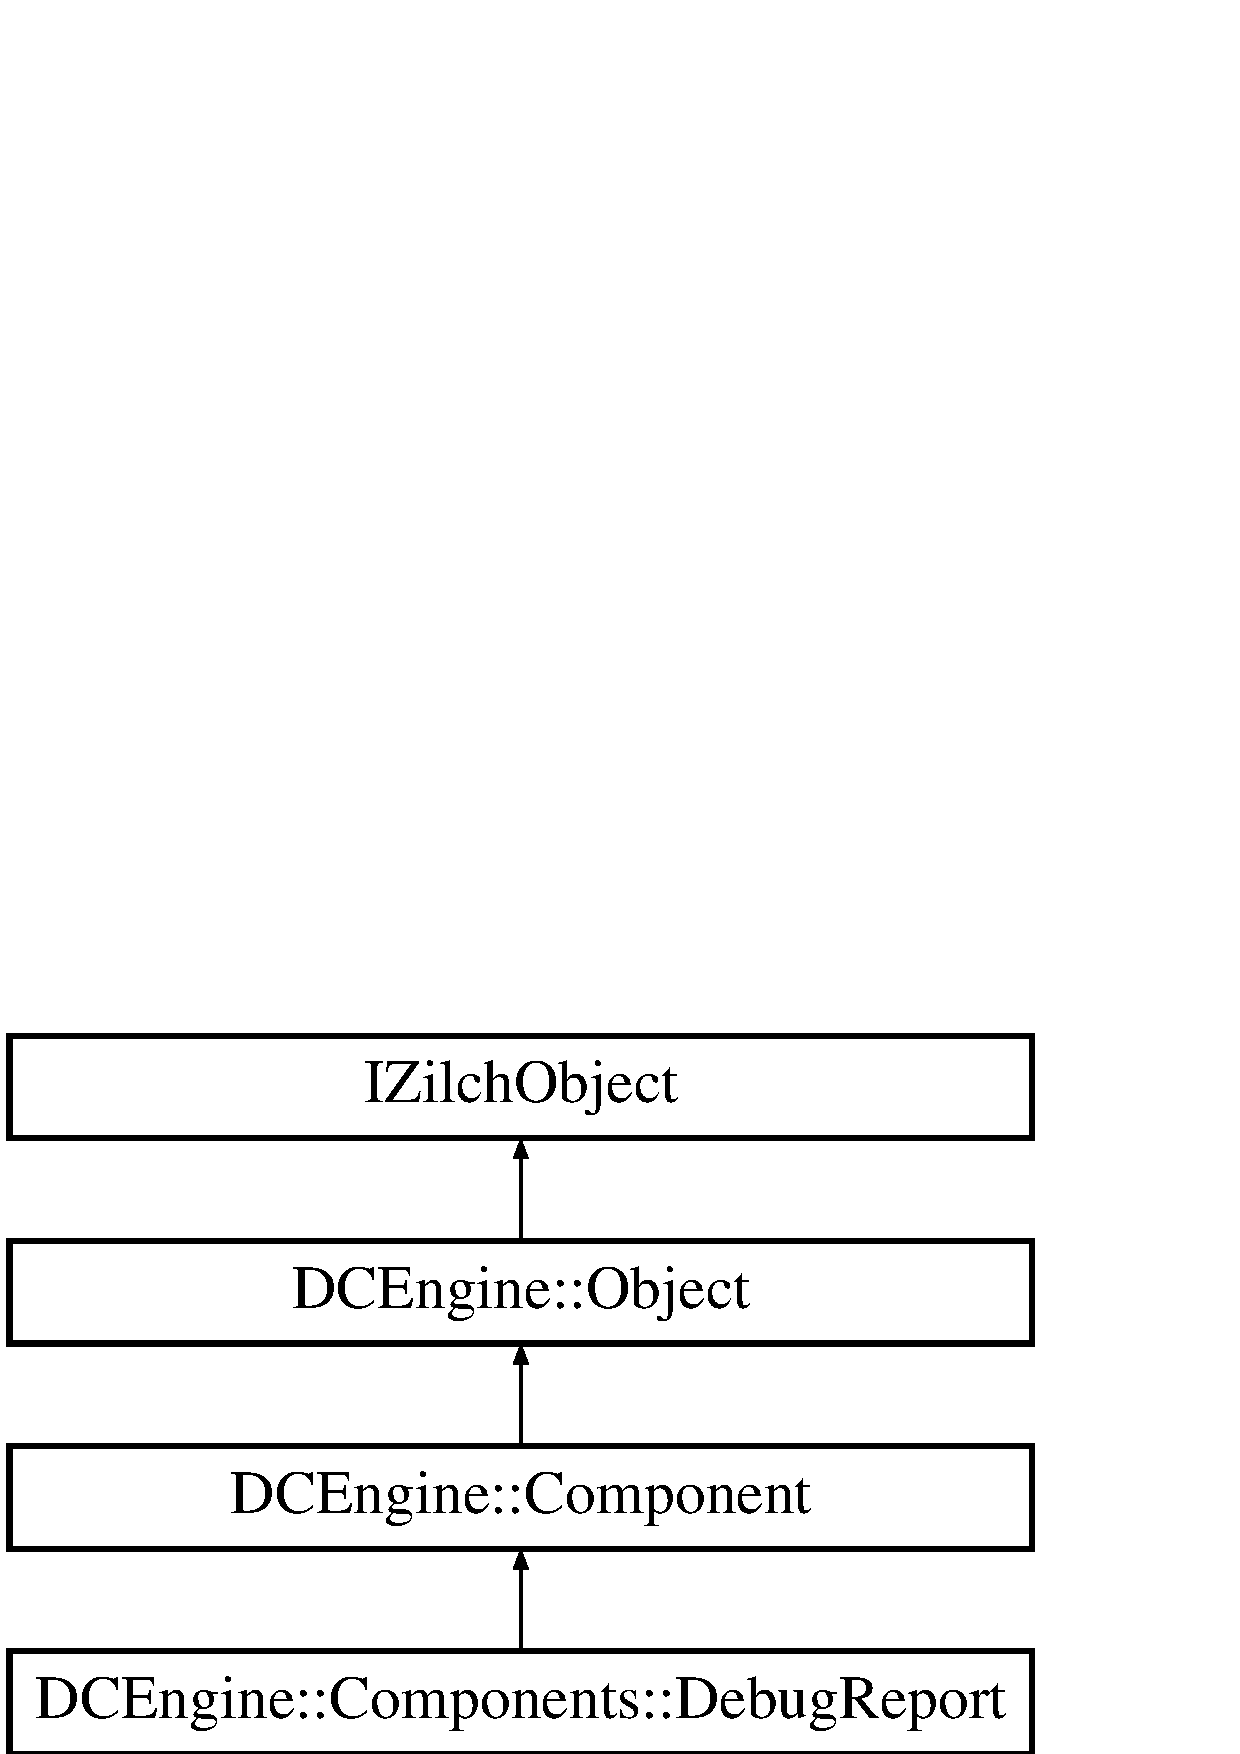
\includegraphics[height=4.000000cm]{classDCEngine_1_1Components_1_1DebugReport}
\end{center}
\end{figure}
\subsection*{Public Member Functions}
\begin{DoxyCompactItemize}
\item 
\hypertarget{classDCEngine_1_1Components_1_1DebugReport_ab78c1ed2ec3b1241694be410e2be3852}{{\bfseries Debug\-Report} (\hyperlink{classDCEngine_1_1Entity}{Entity} \&owner)}\label{classDCEngine_1_1Components_1_1DebugReport_ab78c1ed2ec3b1241694be410e2be3852}

\item 
\hypertarget{classDCEngine_1_1Components_1_1DebugReport_a7e1efd3025921037845f2d1a7e752986}{void {\bfseries Initialize} ()}\label{classDCEngine_1_1Components_1_1DebugReport_a7e1efd3025921037845f2d1a7e752986}

\item 
\hypertarget{classDCEngine_1_1Components_1_1DebugReport_aca3394ed432e4d19364fc8d34f781a36}{virtual void {\bfseries Serialize} (Json\-::\-Value \&root)}\label{classDCEngine_1_1Components_1_1DebugReport_aca3394ed432e4d19364fc8d34f781a36}

\item 
\hypertarget{classDCEngine_1_1Components_1_1DebugReport_a9479a8ee5e72b3a48915f0d7779eee63}{virtual void {\bfseries Deserialize} (Json\-::\-Value \&root)}\label{classDCEngine_1_1Components_1_1DebugReport_a9479a8ee5e72b3a48915f0d7779eee63}

\item 
\hypertarget{classDCEngine_1_1Components_1_1DebugReport_af19f4c53c360264dbb7d6d9315118a5c}{void {\bfseries On\-Key\-Down\-Event} (\hyperlink{classDCEngine_1_1Events_1_1KeyDown}{Events\-::\-Key\-Down} $\ast$event)}\label{classDCEngine_1_1Components_1_1DebugReport_af19f4c53c360264dbb7d6d9315118a5c}

\item 
\hypertarget{classDCEngine_1_1Components_1_1DebugReport_aa982742d1be781ed1f6948ea8036db1b}{void {\bfseries On\-Key\-Up\-Event} (\hyperlink{classDCEngine_1_1Events_1_1KeyUp}{Events\-::\-Key\-Up} $\ast$event)}\label{classDCEngine_1_1Components_1_1DebugReport_aa982742d1be781ed1f6948ea8036db1b}

\item 
\hypertarget{classDCEngine_1_1Components_1_1DebugReport_a3c96c8456be40a51bd94b0feef14a4be}{void {\bfseries On\-Mouse\-Down\-Event} (\hyperlink{classDCEngine_1_1Events_1_1MouseDown}{Events\-::\-Mouse\-Down} $\ast$event)}\label{classDCEngine_1_1Components_1_1DebugReport_a3c96c8456be40a51bd94b0feef14a4be}

\item 
\hypertarget{classDCEngine_1_1Components_1_1DebugReport_a58d365ffcb2638c66cb8f4f799f9ae04}{void {\bfseries On\-Logic\-Update\-Event} (\hyperlink{classDCEngine_1_1Events_1_1LogicUpdate}{Events\-::\-Logic\-Update} $\ast$event)}\label{classDCEngine_1_1Components_1_1DebugReport_a58d365ffcb2638c66cb8f4f799f9ae04}

\item 
\hypertarget{classDCEngine_1_1Components_1_1DebugReport_a923f6c23226ae5823ac6aa650216ff32}{void {\bfseries Debug\-Draw} ()}\label{classDCEngine_1_1Components_1_1DebugReport_a923f6c23226ae5823ac6aa650216ff32}

\end{DoxyCompactItemize}
\subsection*{Public Attributes}
\begin{DoxyCompactItemize}
\item 
\hypertarget{classDCEngine_1_1Components_1_1DebugReport_a0e9fa451136daad9f54c86ab1670233d}{\hyperlink{classDCEngine_1_1Components_1_1Transform}{Transform} $\ast$ {\bfseries Transform\-Component}}\label{classDCEngine_1_1Components_1_1DebugReport_a0e9fa451136daad9f54c86ab1670233d}

\item 
\hypertarget{classDCEngine_1_1Components_1_1DebugReport_a7127dc66cb1ecb1b11e0c73823208739}{Boolean {\bfseries Report\-Translation} = false}\label{classDCEngine_1_1Components_1_1DebugReport_a7127dc66cb1ecb1b11e0c73823208739}

\item 
\hypertarget{classDCEngine_1_1Components_1_1DebugReport_a85849fcbc6567d5a59340bc72279da84}{Debug\-Draw\-Type {\bfseries Draw\-Type} = Debug\-Draw\-Type\-::\-None}\label{classDCEngine_1_1Components_1_1DebugReport_a85849fcbc6567d5a59340bc72279da84}

\item 
\hypertarget{classDCEngine_1_1Components_1_1DebugReport_aea9097f805de22e8f5f26d613ffd3899}{Real {\bfseries Radius} = 1}\label{classDCEngine_1_1Components_1_1DebugReport_aea9097f805de22e8f5f26d613ffd3899}

\item 
\hypertarget{classDCEngine_1_1Components_1_1DebugReport_ae85740dd70834f81c7f3089abb235abc}{Real {\bfseries Height} = 1}\label{classDCEngine_1_1Components_1_1DebugReport_ae85740dd70834f81c7f3089abb235abc}

\item 
\hypertarget{classDCEngine_1_1Components_1_1DebugReport_ac5871b2615855c2279d761b47bac35da}{Vec3 {\bfseries Offset} = Vec3(0, 0, 0)}\label{classDCEngine_1_1Components_1_1DebugReport_ac5871b2615855c2279d761b47bac35da}

\item 
\hypertarget{classDCEngine_1_1Components_1_1DebugReport_af943c965fbf5f529a82623ecd962904a}{Vec4 {\bfseries Color} = Vec4(0.\-5, 0.\-5, 0.\-5, 1)}\label{classDCEngine_1_1Components_1_1DebugReport_af943c965fbf5f529a82623ecd962904a}

\end{DoxyCompactItemize}
\subsection*{Additional Inherited Members}


The documentation for this class was generated from the following files\-:\begin{DoxyCompactItemize}
\item 
Core/\-Components/\hyperlink{DebugReport_8h}{Debug\-Report.\-h}\item 
Core/\-Components/\hyperlink{DebugReport_8cpp}{Debug\-Report.\-cpp}\end{DoxyCompactItemize}

\hypertarget{classDCEngine_1_1Delegate}{\section{D\-C\-Engine\-:\-:Delegate Class Reference}
\label{classDCEngine_1_1Delegate}\index{D\-C\-Engine\-::\-Delegate@{D\-C\-Engine\-::\-Delegate}}
}


The documentation for this class was generated from the following file\-:\begin{DoxyCompactItemize}
\item 
Core/\-Engine/\hyperlink{Delegate_8h}{Delegate.\-h}\end{DoxyCompactItemize}

\hypertarget{classDCEngine_1_1DerivedObject}{\section{D\-C\-Engine\-:\-:Derived\-Object Class Reference}
\label{classDCEngine_1_1DerivedObject}\index{D\-C\-Engine\-::\-Derived\-Object@{D\-C\-Engine\-::\-Derived\-Object}}
}
Inheritance diagram for D\-C\-Engine\-:\-:Derived\-Object\-:\begin{figure}[H]
\begin{center}
\leavevmode
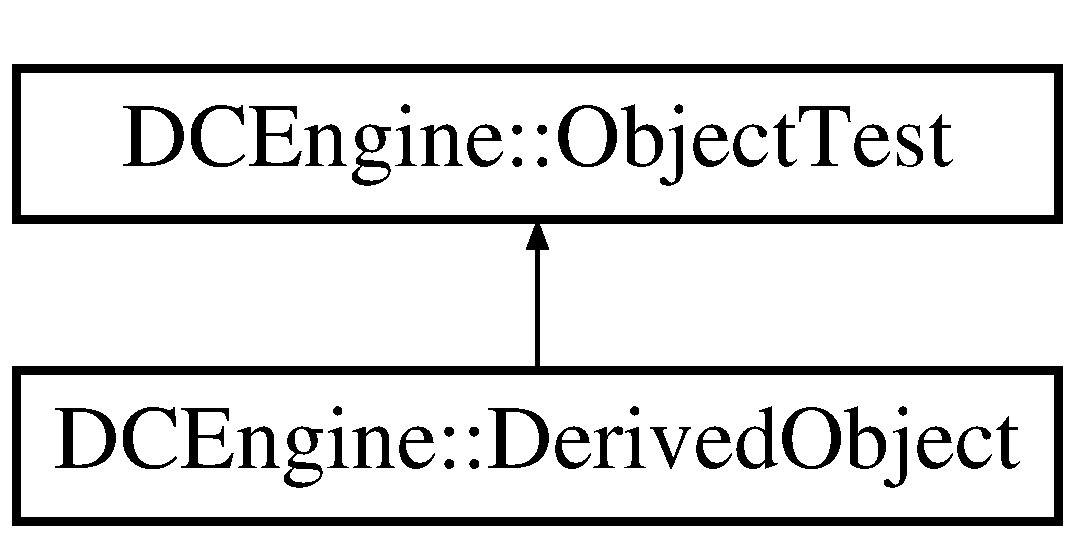
\includegraphics[height=2.000000cm]{classDCEngine_1_1DerivedObject}
\end{center}
\end{figure}
\subsection*{Public Member Functions}
\begin{DoxyCompactItemize}
\item 
\hypertarget{classDCEngine_1_1DerivedObject_a10debf4f7239c670c666e28efd6e6171}{{\bfseries Derived\-Object} (int id)}\label{classDCEngine_1_1DerivedObject_a10debf4f7239c670c666e28efd6e6171}

\item 
\hypertarget{classDCEngine_1_1DerivedObject_a2b82d7ed1f8a1f80161f32da90db7cb4}{{\bfseries M\-E\-T\-A\-\_\-\-A\-D\-D\-\_\-\-C\-L\-A\-S\-S} (\hyperlink{classDCEngine_1_1DerivedObject}{Derived\-Object})}\label{classDCEngine_1_1DerivedObject_a2b82d7ed1f8a1f80161f32da90db7cb4}

\end{DoxyCompactItemize}


The documentation for this class was generated from the following files\-:\begin{DoxyCompactItemize}
\item 
Projects/\-Dollhouse/\hyperlink{ReflectionTest_8h}{Reflection\-Test.\-h}\item 
Projects/\-Dollhouse/Reflection\-Test.\-cpp\end{DoxyCompactItemize}

\hypertarget{structDCEngine_1_1Systems_1_1DetectionPairing}{\section{D\-C\-Engine\-:\-:Systems\-:\-:Detection\-Pairing Struct Reference}
\label{structDCEngine_1_1Systems_1_1DetectionPairing}\index{D\-C\-Engine\-::\-Systems\-::\-Detection\-Pairing@{D\-C\-Engine\-::\-Systems\-::\-Detection\-Pairing}}
}
\subsection*{Public Attributes}
\begin{DoxyCompactItemize}
\item 
\hypertarget{structDCEngine_1_1Systems_1_1DetectionPairing_a4c192316cec5bb95fcc4dae82033cf2f}{\hyperlink{classDCEngine_1_1GameObject}{Game\-Object\-Ptr} {\bfseries obj1} = N\-U\-L\-L}\label{structDCEngine_1_1Systems_1_1DetectionPairing_a4c192316cec5bb95fcc4dae82033cf2f}

\item 
\hypertarget{structDCEngine_1_1Systems_1_1DetectionPairing_ad51ad3626638180701a767d142578c55}{\hyperlink{classDCEngine_1_1GameObject}{Game\-Object\-Ptr} {\bfseries obj2} = N\-U\-L\-L}\label{structDCEngine_1_1Systems_1_1DetectionPairing_ad51ad3626638180701a767d142578c55}

\item 
\hypertarget{structDCEngine_1_1Systems_1_1DetectionPairing_a83f971b28cfa7393729a530ac4f95e94}{\hyperlink{structDCEngine_1_1CollisionFilter}{Collision\-Filter} {\bfseries filter}}\label{structDCEngine_1_1Systems_1_1DetectionPairing_a83f971b28cfa7393729a530ac4f95e94}

\end{DoxyCompactItemize}


The documentation for this struct was generated from the following file\-:\begin{DoxyCompactItemize}
\item 
Core/\-Systems/\-Physics/\hyperlink{Physics_8h}{Physics.\-h}\end{DoxyCompactItemize}

\hypertarget{classDCEngine_1_1DispatchGameEvents}{\section{D\-C\-Engine\-:\-:Dispatch\-Game\-Events Class Reference}
\label{classDCEngine_1_1DispatchGameEvents}\index{D\-C\-Engine\-::\-Dispatch\-Game\-Events@{D\-C\-Engine\-::\-Dispatch\-Game\-Events}}
}
\subsection*{Static Public Member Functions}
\begin{DoxyCompactItemize}
\item 
\hypertarget{classDCEngine_1_1DispatchGameEvents_a3eb1cb43d059358e2796477c8e409e9d}{static void {\bfseries Game\-Focus\-In} ()}\label{classDCEngine_1_1DispatchGameEvents_a3eb1cb43d059358e2796477c8e409e9d}

\item 
\hypertarget{classDCEngine_1_1DispatchGameEvents_a5a498b3d1d6fd33a5e5522c013213bd5}{static void {\bfseries Game\-Focus\-Out} ()}\label{classDCEngine_1_1DispatchGameEvents_a5a498b3d1d6fd33a5e5522c013213bd5}

\item 
\hypertarget{classDCEngine_1_1DispatchGameEvents_ac60b055051d3a81eef85e521aaac14e0}{static void {\bfseries Game\-Load} ()}\label{classDCEngine_1_1DispatchGameEvents_ac60b055051d3a81eef85e521aaac14e0}

\item 
\hypertarget{classDCEngine_1_1DispatchGameEvents_aac5e1417f53d66f2a7aeb1212d9c875c}{static void {\bfseries Game\-Request\-Quit} ()}\label{classDCEngine_1_1DispatchGameEvents_aac5e1417f53d66f2a7aeb1212d9c875c}

\item 
\hypertarget{classDCEngine_1_1DispatchGameEvents_aad7d721d62ffc95a0c66147c91a8ddea}{static void {\bfseries Game\-Started} ()}\label{classDCEngine_1_1DispatchGameEvents_aad7d721d62ffc95a0c66147c91a8ddea}

\item 
\hypertarget{classDCEngine_1_1DispatchGameEvents_ad63bd9040d54088bce0b8796c0fd2df8}{static void {\bfseries Game\-Ended} ()}\label{classDCEngine_1_1DispatchGameEvents_ad63bd9040d54088bce0b8796c0fd2df8}

\item 
\hypertarget{classDCEngine_1_1DispatchGameEvents_a4114723498ea290b2630daf22641b03d}{static void {\bfseries Game\-Setup} ()}\label{classDCEngine_1_1DispatchGameEvents_a4114723498ea290b2630daf22641b03d}

\end{DoxyCompactItemize}


The documentation for this class was generated from the following files\-:\begin{DoxyCompactItemize}
\item 
Core/\-Events/Dispatch\-Game\-Events.\-h\item 
Core/\-Events/\hyperlink{DispatchGameEvents_8cpp}{Dispatch\-Game\-Events.\-cpp}\end{DoxyCompactItemize}

\hypertarget{classDCEngine_1_1Systems_1_1DispatchSystemEvents}{\section{D\-C\-Engine\-:\-:Systems\-:\-:Dispatch\-System\-Events Class Reference}
\label{classDCEngine_1_1Systems_1_1DispatchSystemEvents}\index{D\-C\-Engine\-::\-Systems\-::\-Dispatch\-System\-Events@{D\-C\-Engine\-::\-Systems\-::\-Dispatch\-System\-Events}}
}
\subsection*{Static Public Member Functions}
\begin{DoxyCompactItemize}
\item 
\hypertarget{classDCEngine_1_1Systems_1_1DispatchSystemEvents_a3d48623341b59addca47769faee76a81}{static void {\bfseries Engine\-Resume} ()}\label{classDCEngine_1_1Systems_1_1DispatchSystemEvents_a3d48623341b59addca47769faee76a81}

\item 
\hypertarget{classDCEngine_1_1Systems_1_1DispatchSystemEvents_aaee95eb74012a746d7302a5138f8fb82}{static void {\bfseries Engine\-Pause} ()}\label{classDCEngine_1_1Systems_1_1DispatchSystemEvents_aaee95eb74012a746d7302a5138f8fb82}

\item 
\hypertarget{classDCEngine_1_1Systems_1_1DispatchSystemEvents_ab16d23e0cafd613b91718b40f485ff3d}{static void {\bfseries Engine\-Exit} ()}\label{classDCEngine_1_1Systems_1_1DispatchSystemEvents_ab16d23e0cafd613b91718b40f485ff3d}

\item 
\hypertarget{classDCEngine_1_1Systems_1_1DispatchSystemEvents_a7995d16f3445bb72d8511ef4b71a1a93}{static void {\bfseries Set\-Window\-Caption} (std\-::string name)}\label{classDCEngine_1_1Systems_1_1DispatchSystemEvents_a7995d16f3445bb72d8511ef4b71a1a93}

\item 
\hypertarget{classDCEngine_1_1Systems_1_1DispatchSystemEvents_a7a90d3d900947bf3d792cffdfac645ac}{static void {\bfseries Window\-Lost\-Focus} ()}\label{classDCEngine_1_1Systems_1_1DispatchSystemEvents_a7a90d3d900947bf3d792cffdfac645ac}

\item 
\hypertarget{classDCEngine_1_1Systems_1_1DispatchSystemEvents_aea967101dc7c1e8432804806549c195b}{static void {\bfseries Window\-Gained\-Focus} ()}\label{classDCEngine_1_1Systems_1_1DispatchSystemEvents_aea967101dc7c1e8432804806549c195b}

\end{DoxyCompactItemize}


The documentation for this class was generated from the following files\-:\begin{DoxyCompactItemize}
\item 
Core/\-Systems/\hyperlink{DispatchSystemEvents_8h}{Dispatch\-System\-Events.\-h}\item 
Core/\-Systems/\hyperlink{DispatchSystemEvents_8cpp}{Dispatch\-System\-Events.\-cpp}\end{DoxyCompactItemize}

\hypertarget{classDCEngine_1_1DollHouse}{\section{D\-C\-Engine\-:\-:Doll\-House Class Reference}
\label{classDCEngine_1_1DollHouse}\index{D\-C\-Engine\-::\-Doll\-House@{D\-C\-Engine\-::\-Doll\-House}}
}
Inheritance diagram for D\-C\-Engine\-:\-:Doll\-House\-:\begin{figure}[H]
\begin{center}
\leavevmode
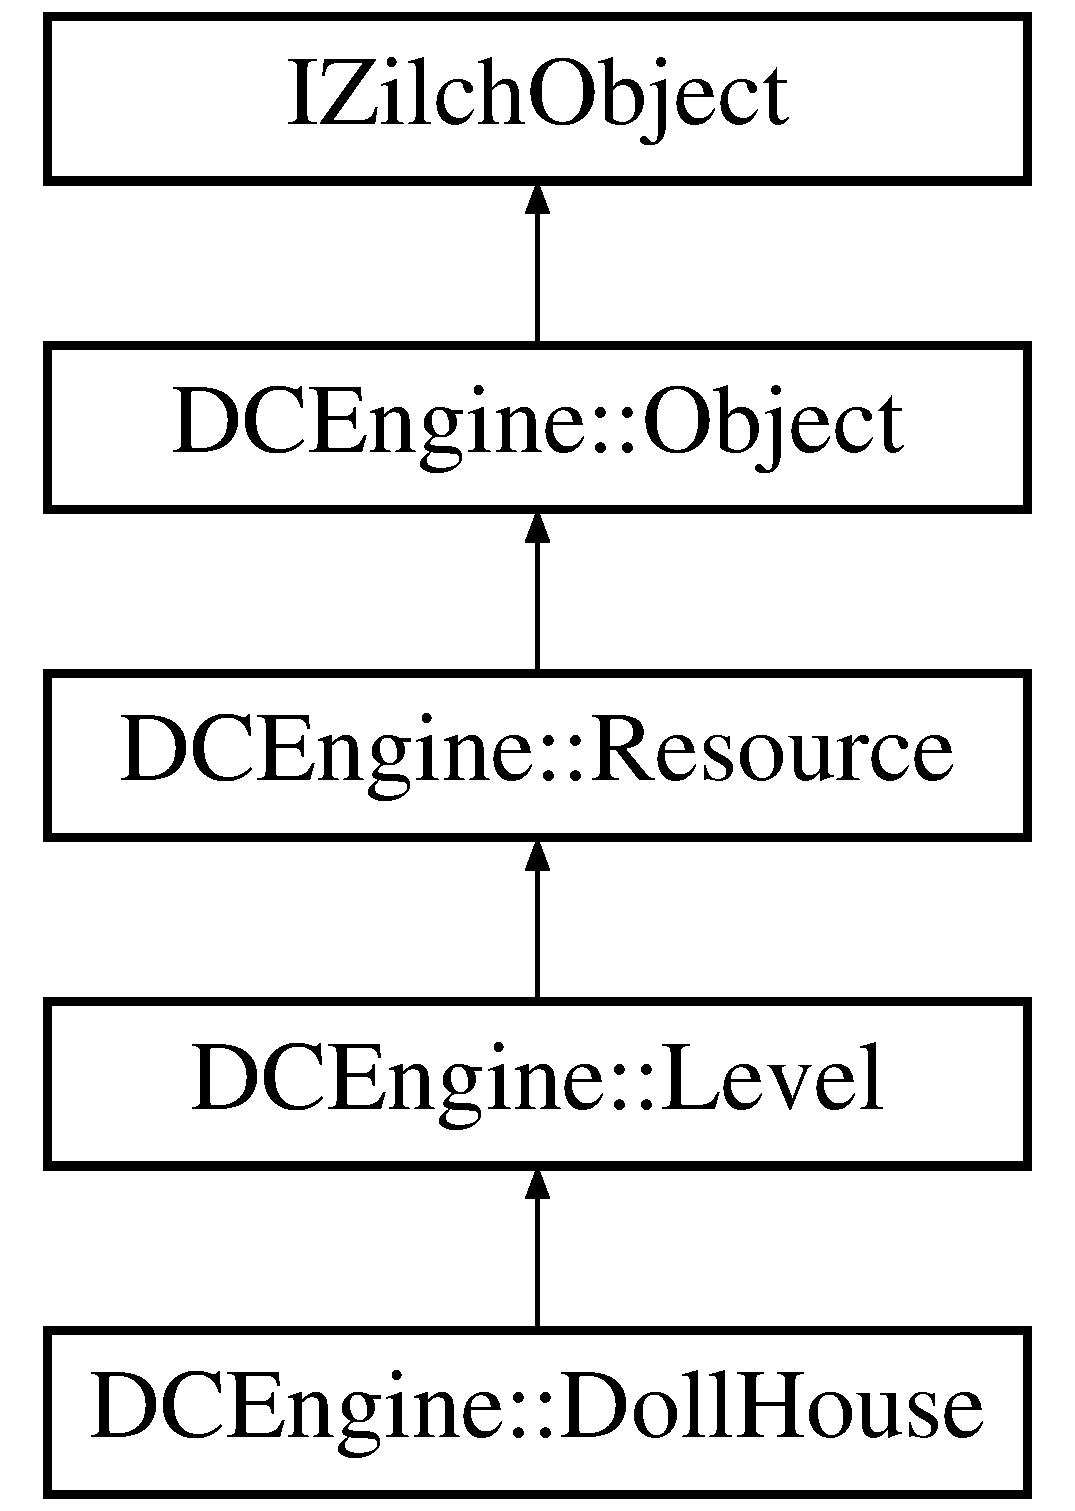
\includegraphics[height=5.000000cm]{classDCEngine_1_1DollHouse}
\end{center}
\end{figure}
\subsection*{Public Member Functions}
\begin{DoxyCompactItemize}
\item 
\hypertarget{classDCEngine_1_1DollHouse_a2e74c227d1a107a35c0d2166884f9009}{{\bfseries Doll\-House} (\hyperlink{classDCEngine_1_1Space}{Space} \&space, \hyperlink{classDCEngine_1_1GameSession}{Game\-Session} \&gamesession)}\label{classDCEngine_1_1DollHouse_a2e74c227d1a107a35c0d2166884f9009}

\item 
\hypertarget{classDCEngine_1_1DollHouse_af366b869a9ffe11f143a30d164489a58}{void {\bfseries Setup\-Camera} ()}\label{classDCEngine_1_1DollHouse_af366b869a9ffe11f143a30d164489a58}

\item 
\hypertarget{classDCEngine_1_1DollHouse_a265608cde0beeabeeea3b6c1c7057f3c}{void {\bfseries Serialize\-Test} ()}\label{classDCEngine_1_1DollHouse_a265608cde0beeabeeea3b6c1c7057f3c}

\item 
\hypertarget{classDCEngine_1_1DollHouse_abe570d2358679c6ea4173615b89d222f}{\hyperlink{classDCEngine_1_1GameObject}{Game\-Object\-Ptr} {\bfseries Construct\-Game\-Object} (std\-::string name)}\label{classDCEngine_1_1DollHouse_abe570d2358679c6ea4173615b89d222f}

\item 
\hypertarget{classDCEngine_1_1DollHouse_a747a009e50a3b8ba06cb008b825020a7}{void {\bfseries Game\-Objects} ()}\label{classDCEngine_1_1DollHouse_a747a009e50a3b8ba06cb008b825020a7}

\item 
\hypertarget{classDCEngine_1_1DollHouse_a446989e020945448a15e3b6bdcc3c4f1}{void {\bfseries Setup\-Background} ()}\label{classDCEngine_1_1DollHouse_a446989e020945448a15e3b6bdcc3c4f1}

\item 
void \hyperlink{classDCEngine_1_1DollHouse_aa95ff0381366798633318e9d25dd17a2}{Environment\-Setup} ()
\item 
\hypertarget{classDCEngine_1_1DollHouse_a1233fd14eeb65b3c07b996ea337c82ea}{void {\bfseries Generate\-Random\-Jumper\-Enemy} (Vec3 translation, Vec3 scale, Vec4 color)}\label{classDCEngine_1_1DollHouse_a1233fd14eeb65b3c07b996ea337c82ea}

\item 
\hypertarget{classDCEngine_1_1DollHouse_a18ad62bc3e68faefe70c40f80d514a8b}{void {\bfseries Generate\-Basic\-Chaser\-Enemy} (Vec3 translation, Vec3 scale, Vec4 color, Real patrol\-Range)}\label{classDCEngine_1_1DollHouse_a18ad62bc3e68faefe70c40f80d514a8b}

\item 
\hypertarget{classDCEngine_1_1DollHouse_a2238a493d2e6e67341ba26811f0b6f2b}{void {\bfseries Generate\-Terrain} (Vec3 translation, Vec3 scale, Vec4 color)}\label{classDCEngine_1_1DollHouse_a2238a493d2e6e67341ba26811f0b6f2b}

\item 
\hypertarget{classDCEngine_1_1DollHouse_ac7c24fd22eb5fb08d11d3e69dc54608a}{void {\bfseries Generate\-Hazard\-Area} (Vec3 translation, Vec3 scale, Vec4 color)}\label{classDCEngine_1_1DollHouse_ac7c24fd22eb5fb08d11d3e69dc54608a}

\item 
\hypertarget{classDCEngine_1_1DollHouse_a7e7e177fcfe7976a0695fd4e5879eedb}{void {\bfseries Generate\-Player} (Vec3 translation, Vec3 scale, Vec4 color)}\label{classDCEngine_1_1DollHouse_a7e7e177fcfe7976a0695fd4e5879eedb}

\item 
\hypertarget{classDCEngine_1_1DollHouse_a5d28b6a03791c8c29aea57cbb1939390}{void {\bfseries Generate\-Ball} (Vec3 translation, Vec3 scale, Vec4 color)}\label{classDCEngine_1_1DollHouse_a5d28b6a03791c8c29aea57cbb1939390}

\item 
\hypertarget{classDCEngine_1_1DollHouse_a5538d70afb2a893240e2f91ab6818366}{void {\bfseries Generate\-Camera} (Vec3 translation, Vec3 scale, Vec4 color)}\label{classDCEngine_1_1DollHouse_a5538d70afb2a893240e2f91ab6818366}

\item 
\hypertarget{classDCEngine_1_1DollHouse_a5bb89933b7c39489db9b0e8c110c6011}{void {\bfseries Generate\-Freeze\-Enabler} (Vec3 translation, Vec3 scale, Vec4 color)}\label{classDCEngine_1_1DollHouse_a5bb89933b7c39489db9b0e8c110c6011}

\item 
\hypertarget{classDCEngine_1_1DollHouse_a54e7a7b4ef7a7b41931ef9eb69ab0494}{void {\bfseries Generate\-Button} (Vec3 translation, Vec3 scale, Vec4 color)}\label{classDCEngine_1_1DollHouse_a54e7a7b4ef7a7b41931ef9eb69ab0494}

\end{DoxyCompactItemize}
\subsection*{Public Attributes}
\begin{DoxyCompactItemize}
\item 
\hypertarget{classDCEngine_1_1DollHouse_a0969084f4d453cc694fc7f79ba384f51}{int {\bfseries Terrain\-Pieces\-Created} = 0}\label{classDCEngine_1_1DollHouse_a0969084f4d453cc694fc7f79ba384f51}

\item 
\hypertarget{classDCEngine_1_1DollHouse_af7ae7dbf64986d7dcb1dfa782acc3565}{\hyperlink{classDCEngine_1_1GameObject}{Game\-Object\-Ptr} {\bfseries doll}}\label{classDCEngine_1_1DollHouse_af7ae7dbf64986d7dcb1dfa782acc3565}

\item 
\hypertarget{classDCEngine_1_1DollHouse_a3b16201e1ac82d001660ae5add0611c6}{\hyperlink{classDCEngine_1_1GameObject}{Game\-Object\-Ptr} {\bfseries camera\-Obj}}\label{classDCEngine_1_1DollHouse_a3b16201e1ac82d001660ae5add0611c6}

\item 
\hypertarget{classDCEngine_1_1DollHouse_a93da1408bafe1f9a9e8bcd2edc6bd88d}{\hyperlink{classDCEngine_1_1Space}{Space} $\ast$ {\bfseries space\-\_\-}}\label{classDCEngine_1_1DollHouse_a93da1408bafe1f9a9e8bcd2edc6bd88d}

\item 
\hypertarget{classDCEngine_1_1DollHouse_a630c9fde026c9580ec01830391d9f885}{\hyperlink{classDCEngine_1_1GameSession}{Game\-Session} $\ast$ {\bfseries gamesession\-\_\-}}\label{classDCEngine_1_1DollHouse_a630c9fde026c9580ec01830391d9f885}

\end{DoxyCompactItemize}
\subsection*{Additional Inherited Members}


\subsection{Member Function Documentation}
\hypertarget{classDCEngine_1_1DollHouse_aa95ff0381366798633318e9d25dd17a2}{\index{D\-C\-Engine\-::\-Doll\-House@{D\-C\-Engine\-::\-Doll\-House}!Environment\-Setup@{Environment\-Setup}}
\index{Environment\-Setup@{Environment\-Setup}!DCEngine::DollHouse@{D\-C\-Engine\-::\-Doll\-House}}
\subsubsection[{Environment\-Setup}]{\setlength{\rightskip}{0pt plus 5cm}void D\-C\-Engine\-::\-Doll\-House\-::\-Environment\-Setup (
\begin{DoxyParamCaption}
{}
\end{DoxyParamCaption}
)}}\label{classDCEngine_1_1DollHouse_aa95ff0381366798633318e9d25dd17a2}

\begin{DoxyItemize}
\item Foreground Layer $\ast$/ 
\end{DoxyItemize}

The documentation for this class was generated from the following files\-:\begin{DoxyCompactItemize}
\item 
Projects/\-Dollhouse/\hyperlink{Dollhouse_8h}{Dollhouse.\-h}\item 
Projects/\-Dollhouse/\hyperlink{Background_8cpp}{Background.\-cpp}\item 
Projects/\-Dollhouse/\hyperlink{Environment_8cpp}{Environment.\-cpp}\item 
Projects/\-Dollhouse/\hyperlink{GameObjects_8cpp}{Game\-Objects.\-cpp}\end{DoxyCompactItemize}

\hypertarget{classDCEngine_1_1DrawCircleObj}{\section{D\-C\-Engine\-:\-:Draw\-Circle\-Obj Class Reference}
\label{classDCEngine_1_1DrawCircleObj}\index{D\-C\-Engine\-::\-Draw\-Circle\-Obj@{D\-C\-Engine\-::\-Draw\-Circle\-Obj}}
}
Inheritance diagram for D\-C\-Engine\-:\-:Draw\-Circle\-Obj\-:\begin{figure}[H]
\begin{center}
\leavevmode
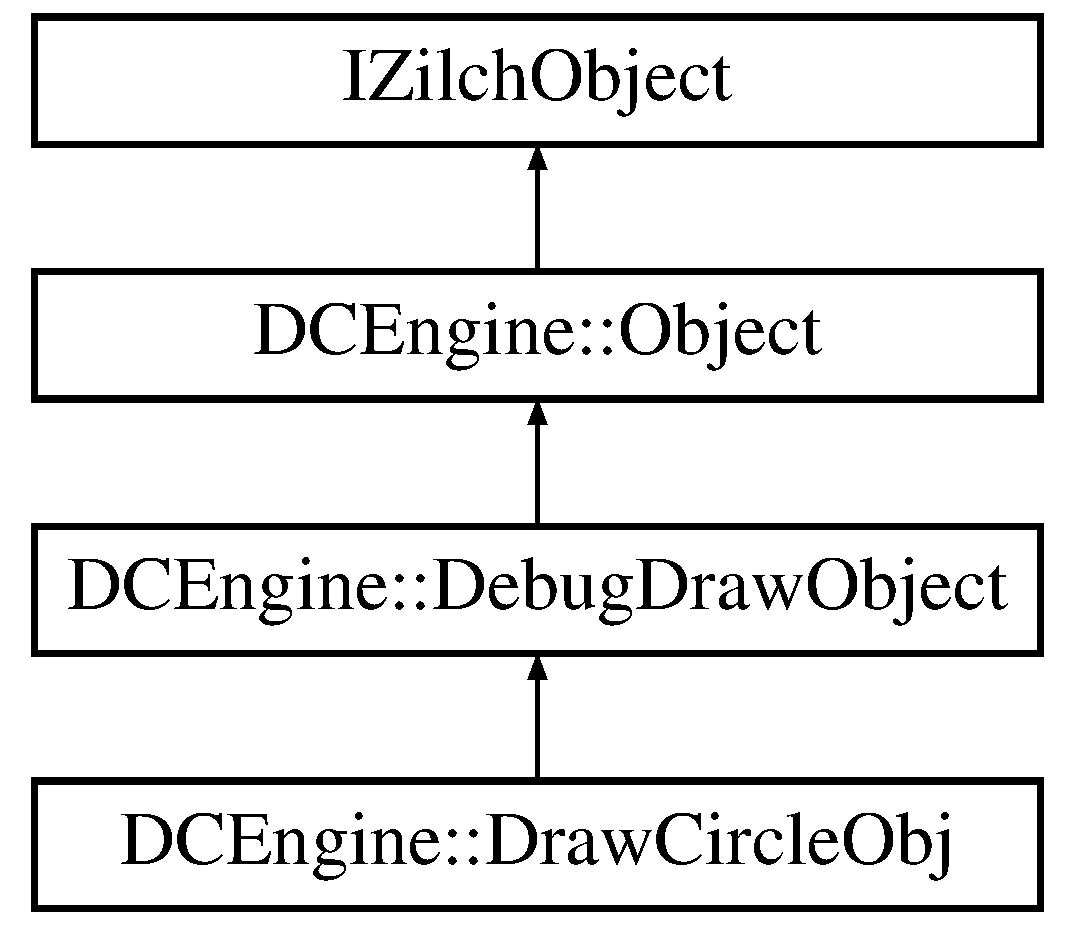
\includegraphics[height=4.000000cm]{classDCEngine_1_1DrawCircleObj}
\end{center}
\end{figure}
\subsection*{Additional Inherited Members}


The documentation for this class was generated from the following file\-:\begin{DoxyCompactItemize}
\item 
Core/\-Objects/\-Debug\-Draw/\hyperlink{DrawCircle_8h}{Draw\-Circle.\-h}\end{DoxyCompactItemize}

\hypertarget{classDCEngine_1_1DrawLineObj}{\section{D\-C\-Engine\-:\-:Draw\-Line\-Obj Class Reference}
\label{classDCEngine_1_1DrawLineObj}\index{D\-C\-Engine\-::\-Draw\-Line\-Obj@{D\-C\-Engine\-::\-Draw\-Line\-Obj}}
}
Inheritance diagram for D\-C\-Engine\-:\-:Draw\-Line\-Obj\-:\begin{figure}[H]
\begin{center}
\leavevmode
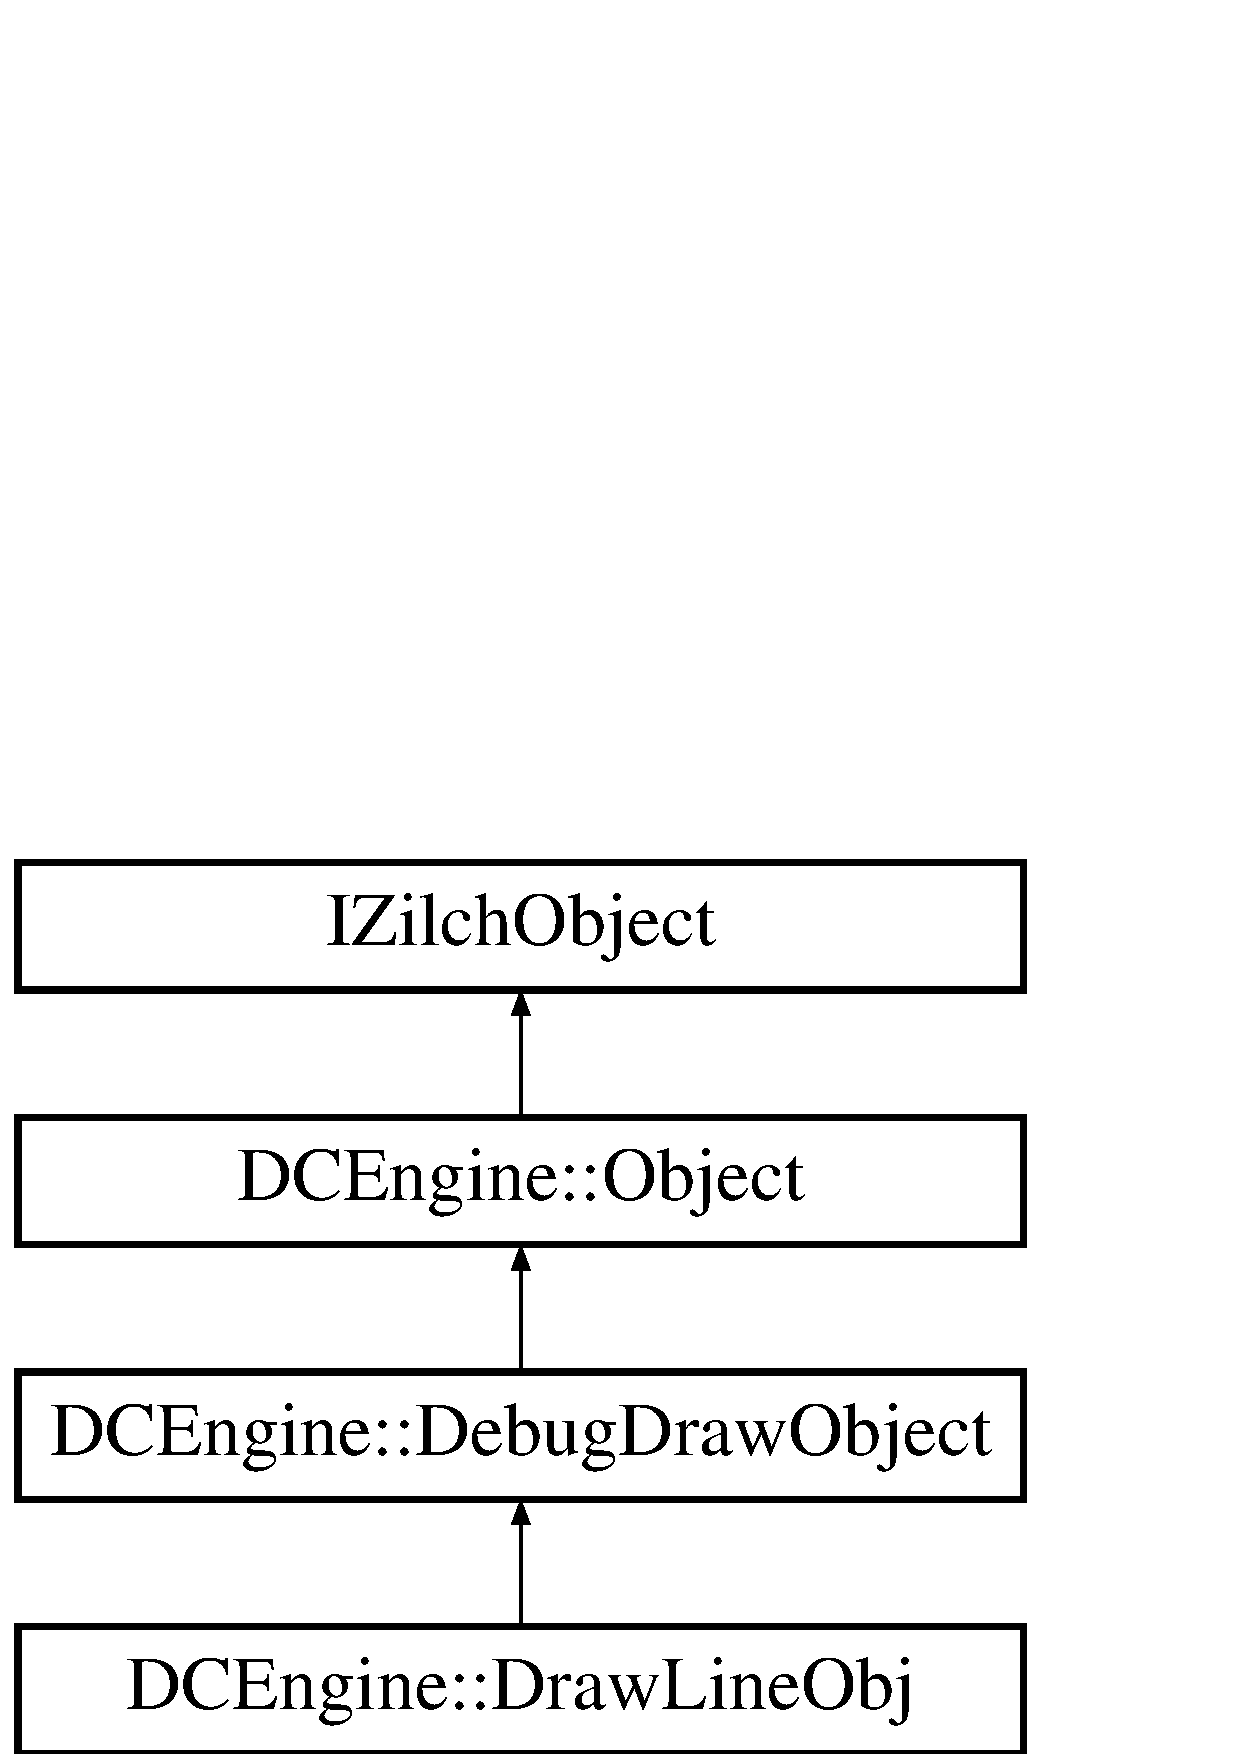
\includegraphics[height=4.000000cm]{classDCEngine_1_1DrawLineObj}
\end{center}
\end{figure}
\subsection*{Public Attributes}
\begin{DoxyCompactItemize}
\item 
\hypertarget{classDCEngine_1_1DrawLineObj_aeed7472194b1a3a970b7bda53cccffb3}{Vec3 {\bfseries Start\-Pos}}\label{classDCEngine_1_1DrawLineObj_aeed7472194b1a3a970b7bda53cccffb3}

\item 
\hypertarget{classDCEngine_1_1DrawLineObj_a601d52b836d18c4dc77d2eb9cdad75bf}{Vec3 {\bfseries End\-Pos}}\label{classDCEngine_1_1DrawLineObj_a601d52b836d18c4dc77d2eb9cdad75bf}

\item 
\hypertarget{classDCEngine_1_1DrawLineObj_aa54282be4d93fd2bea3dde107c124b54}{Real {\bfseries Length}}\label{classDCEngine_1_1DrawLineObj_aa54282be4d93fd2bea3dde107c124b54}

\item 
\hypertarget{classDCEngine_1_1DrawLineObj_adb67601ab8da8e333db65ba67964f69f}{Vec4 {\bfseries Color}}\label{classDCEngine_1_1DrawLineObj_adb67601ab8da8e333db65ba67964f69f}

\end{DoxyCompactItemize}
\subsection*{Additional Inherited Members}


The documentation for this class was generated from the following file\-:\begin{DoxyCompactItemize}
\item 
Core/\-Objects/\-Debug\-Draw/\hyperlink{DrawLine_8h}{Draw\-Line.\-h}\end{DoxyCompactItemize}

\hypertarget{classDCEngine_1_1DrawRectObj}{\section{D\-C\-Engine\-:\-:Draw\-Rect\-Obj Class Reference}
\label{classDCEngine_1_1DrawRectObj}\index{D\-C\-Engine\-::\-Draw\-Rect\-Obj@{D\-C\-Engine\-::\-Draw\-Rect\-Obj}}
}
Inheritance diagram for D\-C\-Engine\-:\-:Draw\-Rect\-Obj\-:\begin{figure}[H]
\begin{center}
\leavevmode
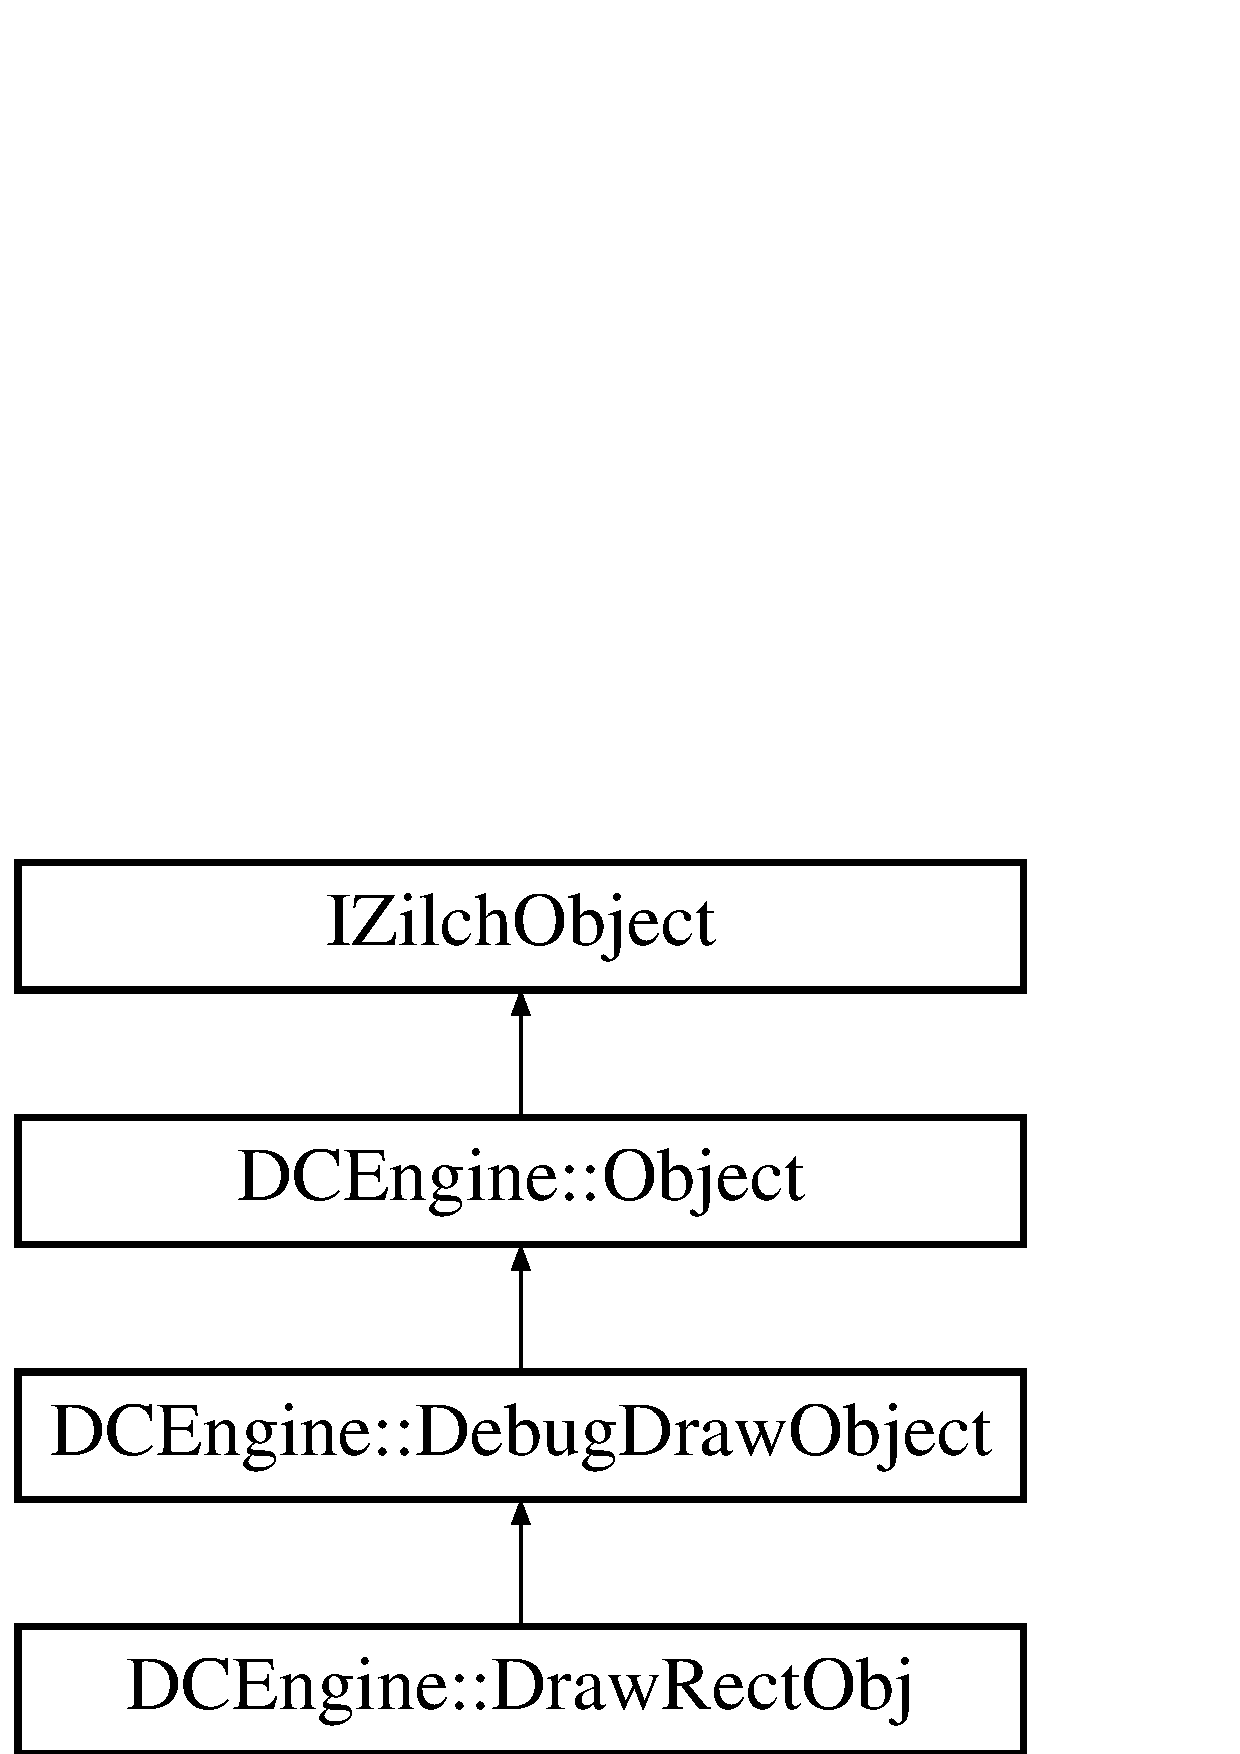
\includegraphics[height=4.000000cm]{classDCEngine_1_1DrawRectObj}
\end{center}
\end{figure}
\subsection*{Additional Inherited Members}


The documentation for this class was generated from the following file\-:\begin{DoxyCompactItemize}
\item 
Core/\-Objects/\-Debug\-Draw/\hyperlink{DrawRectangle_8h}{Draw\-Rectangle.\-h}\end{DoxyCompactItemize}

\hypertarget{classDCEngine_1_1Systems_1_1Editor}{\section{D\-C\-Engine\-:\-:Systems\-:\-:Editor Class Reference}
\label{classDCEngine_1_1Systems_1_1Editor}\index{D\-C\-Engine\-::\-Systems\-::\-Editor@{D\-C\-Engine\-::\-Systems\-::\-Editor}}
}
Inheritance diagram for D\-C\-Engine\-:\-:Systems\-:\-:Editor\-:\begin{figure}[H]
\begin{center}
\leavevmode
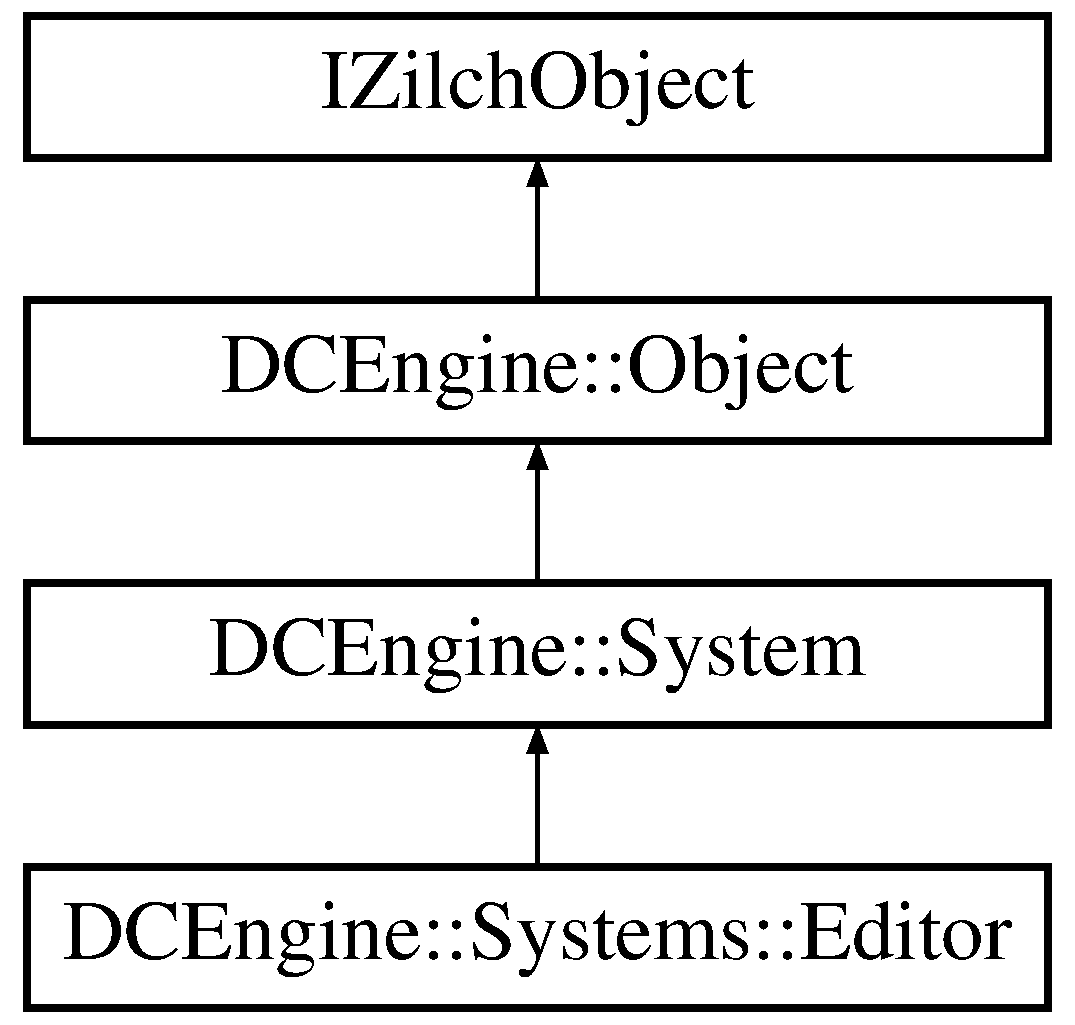
\includegraphics[height=4.000000cm]{classDCEngine_1_1Systems_1_1Editor}
\end{center}
\end{figure}
\subsection*{Public Types}
\begin{DoxyCompactItemize}
\item 
enum {\bfseries Editor\-Tool} \{ \\*
{\bfseries None}, 
{\bfseries Select}, 
{\bfseries Translate}, 
{\bfseries Rotate}, 
\\*
{\bfseries Scale}
 \}
\end{DoxyCompactItemize}
\subsection*{Public Member Functions}
\begin{DoxyCompactItemize}
\item 
\hypertarget{classDCEngine_1_1Systems_1_1Editor_ad37c7860a505ab36f24022ced1cbd99d}{bool \hyperlink{classDCEngine_1_1Systems_1_1Editor_ad37c7860a505ab36f24022ced1cbd99d}{Is\-Enabled} ()}\label{classDCEngine_1_1Systems_1_1Editor_ad37c7860a505ab36f24022ced1cbd99d}

\begin{DoxyCompactList}\small\item\em Returns the current state of the editor. \end{DoxyCompactList}\item 
\hypertarget{classDCEngine_1_1Systems_1_1Editor_afe3f666eb65969922feb62a0f7c09d7d}{void \hyperlink{classDCEngine_1_1Systems_1_1Editor_afe3f666eb65969922feb62a0f7c09d7d}{Toggle\-Editor} ()}\label{classDCEngine_1_1Systems_1_1Editor_afe3f666eb65969922feb62a0f7c09d7d}

\begin{DoxyCompactList}\small\item\em Toggled the \hyperlink{classDCEngine_1_1Systems_1_1Editor}{Editor} on and off. \end{DoxyCompactList}\item 
\hypertarget{classDCEngine_1_1Systems_1_1Editor_ad816896b9358dce4db8ef83d51df5c6d}{void \hyperlink{classDCEngine_1_1Systems_1_1Editor_ad816896b9358dce4db8ef83d51df5c6d}{Toggle\-Editor} (bool)}\label{classDCEngine_1_1Systems_1_1Editor_ad816896b9358dce4db8ef83d51df5c6d}

\begin{DoxyCompactList}\small\item\em Toggles the editor on and off. \end{DoxyCompactList}\item 
void \hyperlink{classDCEngine_1_1Systems_1_1Editor_a4d530af60faddb7e243bcdd21e58d973}{Toggle\-Test} ()
\begin{DoxyCompactList}\small\item\em Toggles the Im\-Gui Test \hyperlink{classDCEngine_1_1Systems_1_1Window}{Window} on and off. \end{DoxyCompactList}\end{DoxyCompactItemize}
\subsection*{Friends}
\begin{DoxyCompactItemize}
\item 
\hypertarget{classDCEngine_1_1Systems_1_1Editor_a3e1914489e4bed4f9f23cdeab34a43dc}{class {\bfseries Engine}}\label{classDCEngine_1_1Systems_1_1Editor_a3e1914489e4bed4f9f23cdeab34a43dc}

\end{DoxyCompactItemize}
\subsection*{Additional Inherited Members}


\subsection{Member Function Documentation}
\hypertarget{classDCEngine_1_1Systems_1_1Editor_a4d530af60faddb7e243bcdd21e58d973}{\index{D\-C\-Engine\-::\-Systems\-::\-Editor@{D\-C\-Engine\-::\-Systems\-::\-Editor}!Toggle\-Test@{Toggle\-Test}}
\index{Toggle\-Test@{Toggle\-Test}!DCEngine::Systems::Editor@{D\-C\-Engine\-::\-Systems\-::\-Editor}}
\subsubsection[{Toggle\-Test}]{\setlength{\rightskip}{0pt plus 5cm}void D\-C\-Engine\-::\-Systems\-::\-Editor\-::\-Toggle\-Test (
\begin{DoxyParamCaption}
{}
\end{DoxyParamCaption}
)}}\label{classDCEngine_1_1Systems_1_1Editor_a4d530af60faddb7e243bcdd21e58d973}


Toggles the Im\-Gui Test \hyperlink{classDCEngine_1_1Systems_1_1Window}{Window} on and off. 

\begin{DoxyRefDesc}{Todo}
\item[\hyperlink{todo__todo000019}{Todo}]Switch to using a stack of active windows rather than this hackery. \end{DoxyRefDesc}


The documentation for this class was generated from the following files\-:\begin{DoxyCompactItemize}
\item 
Core/\-Systems/\-Editor/\hyperlink{Editor_8h}{Editor.\-h}\item 
Core/\-Systems/\-Editor/Camera\-Control.\-cpp\item 
Core/\-Systems/\-Editor/\hyperlink{Diagnostics_8cpp}{Diagnostics.\-cpp}\item 
Core/\-Systems/\-Editor/Editor.\-cpp\item 
Core/\-Systems/\-Editor/\hyperlink{EditorTools_8cpp}{Editor\-Tools.\-cpp}\item 
Core/\-Systems/\-Editor/\hyperlink{EditorToolsDraw_8cpp}{Editor\-Tools\-Draw.\-cpp}\item 
Core/\-Systems/\-Editor/\hyperlink{Levels_8cpp}{Levels.\-cpp}\item 
Core/\-Systems/\-Editor/\hyperlink{Library_8cpp}{Library.\-cpp}\item 
Core/\-Systems/\-Editor/\hyperlink{MainMenu_8cpp}{Main\-Menu.\-cpp}\item 
Core/\-Systems/\-Editor/Menu\-Commands.\-cpp\item 
Core/\-Systems/\-Editor/Menu\-Create.\-cpp\item 
Core/\-Systems/\-Editor/\hyperlink{MenuLaunch_8cpp}{Menu\-Launch.\-cpp}\item 
Core/\-Systems/\-Editor/\hyperlink{MenuProject_8cpp}{Menu\-Project.\-cpp}\item 
Core/\-Systems/\-Editor/Menu\-Select.\-cpp\item 
Core/\-Systems/\-Editor/\hyperlink{Objects_8cpp}{Objects.\-cpp}\item 
Core/\-Systems/\-Editor/\hyperlink{Properties_8cpp}{Properties.\-cpp}\item 
Core/\-Systems/\-Editor/\hyperlink{PropertiesSelect_8cpp}{Properties\-Select.\-cpp}\item 
Core/\-Systems/\-Editor/\hyperlink{ResourceEditors_8cpp}{Resource\-Editors.\-cpp}\item 
Core/\-Systems/\-Editor/Resources.\-cpp\item 
Core/\-Systems/\-Editor/\hyperlink{ResourcesAdd_8cpp}{Resources\-Add.\-cpp}\item 
Core/\-Systems/\-Editor/\hyperlink{WindowConsole_8cpp}{Window\-Console.\-cpp}\item 
Core/\-Systems/\-Editor/Window\-Create.\-cpp\item 
Core/\-Systems/\-Editor/\hyperlink{WindowTools_8cpp}{Window\-Tools.\-cpp}\end{DoxyCompactItemize}

\hypertarget{classDCEngine_1_1Components_1_1EditorCameraController}{\section{D\-C\-Engine\-:\-:Components\-:\-:Editor\-Camera\-Controller Class Reference}
\label{classDCEngine_1_1Components_1_1EditorCameraController}\index{D\-C\-Engine\-::\-Components\-::\-Editor\-Camera\-Controller@{D\-C\-Engine\-::\-Components\-::\-Editor\-Camera\-Controller}}
}
Inheritance diagram for D\-C\-Engine\-:\-:Components\-:\-:Editor\-Camera\-Controller\-:\begin{figure}[H]
\begin{center}
\leavevmode
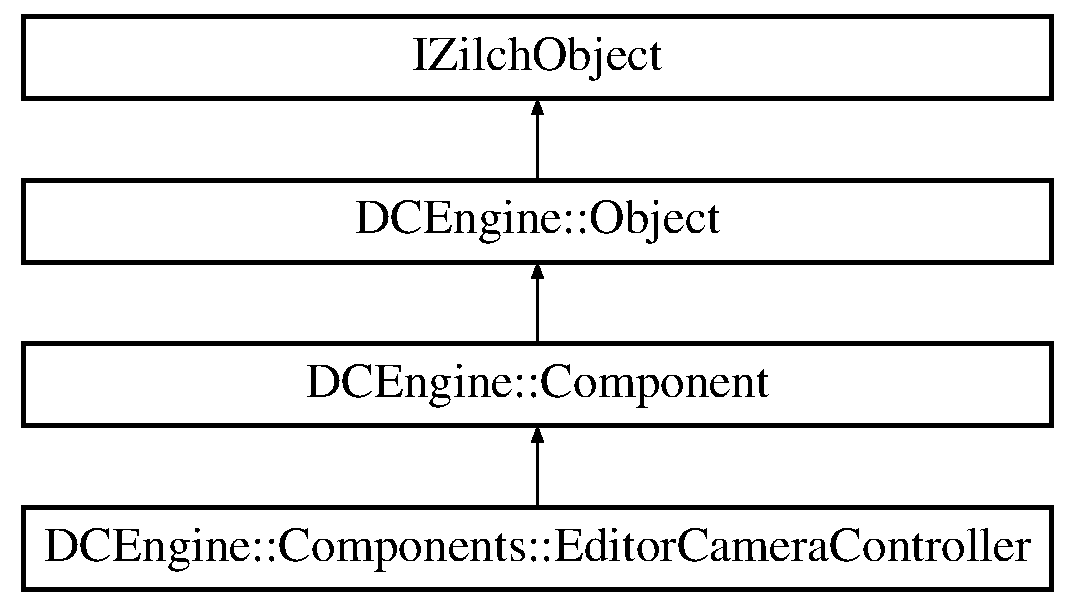
\includegraphics[height=4.000000cm]{classDCEngine_1_1Components_1_1EditorCameraController}
\end{center}
\end{figure}
\subsection*{Public Member Functions}
\begin{DoxyCompactItemize}
\item 
\hypertarget{classDCEngine_1_1Components_1_1EditorCameraController_a2ebbaceafbc264fcfec471d3697c5ecd}{{\bfseries Zilch\-Declare\-Derived\-Type} (\hyperlink{classDCEngine_1_1Components_1_1EditorCameraController}{Editor\-Camera\-Controller}, \hyperlink{classDCEngine_1_1Component}{Component})}\label{classDCEngine_1_1Components_1_1EditorCameraController_a2ebbaceafbc264fcfec471d3697c5ecd}

\item 
\hypertarget{classDCEngine_1_1Components_1_1EditorCameraController_a5b461a9365e428f83d0f661899f9a859}{{\bfseries D\-C\-E\-\_\-\-D\-E\-F\-I\-N\-E\-\_\-\-P\-R\-O\-P\-E\-R\-T\-Y} (Real, Move\-Speed)}\label{classDCEngine_1_1Components_1_1EditorCameraController_a5b461a9365e428f83d0f661899f9a859}

\item 
\hypertarget{classDCEngine_1_1Components_1_1EditorCameraController_ab3ed0ec14ef4c9b849efbb7b2310e6d5}{{\bfseries D\-C\-E\-\_\-\-D\-E\-F\-I\-N\-E\-\_\-\-P\-R\-O\-P\-E\-R\-T\-Y} (Real, Rot\-Speed)}\label{classDCEngine_1_1Components_1_1EditorCameraController_ab3ed0ec14ef4c9b849efbb7b2310e6d5}

\item 
\hypertarget{classDCEngine_1_1Components_1_1EditorCameraController_a0ef29bd91540b99c4d32b5507c9e1c7a}{{\bfseries D\-C\-E\-\_\-\-D\-E\-F\-I\-N\-E\-\_\-\-P\-R\-O\-P\-E\-R\-T\-Y} (Real, Zoom\-Speed)}\label{classDCEngine_1_1Components_1_1EditorCameraController_a0ef29bd91540b99c4d32b5507c9e1c7a}

\item 
\hypertarget{classDCEngine_1_1Components_1_1EditorCameraController_ab0b3fb16ca4bdf1ae8f54fe2026c348f}{{\bfseries Editor\-Camera\-Controller} (\hyperlink{classDCEngine_1_1Entity}{Entity} \&owner)}\label{classDCEngine_1_1Components_1_1EditorCameraController_ab0b3fb16ca4bdf1ae8f54fe2026c348f}

\item 
\hypertarget{classDCEngine_1_1Components_1_1EditorCameraController_a4e820d4b60712d5d57153a29dffd7cb0}{void \hyperlink{classDCEngine_1_1Components_1_1EditorCameraController_a4e820d4b60712d5d57153a29dffd7cb0}{Initialize} ()}\label{classDCEngine_1_1Components_1_1EditorCameraController_a4e820d4b60712d5d57153a29dffd7cb0}

\begin{DoxyCompactList}\small\item\em Initializes the \hyperlink{classDCEngine_1_1Components_1_1EditorCameraController}{Editor\-Camera\-Controller}. \end{DoxyCompactList}\item 
\hypertarget{classDCEngine_1_1Components_1_1EditorCameraController_a41ae801d449a38d59fc664ed8d195d26}{void {\bfseries On\-Key\-Down\-Event} (\hyperlink{classDCEngine_1_1Events_1_1KeyDown}{Events\-::\-Key\-Down} $\ast$event)}\label{classDCEngine_1_1Components_1_1EditorCameraController_a41ae801d449a38d59fc664ed8d195d26}

\item 
\hypertarget{classDCEngine_1_1Components_1_1EditorCameraController_a87bb1582402019f45d3f3d9ab00217e9}{void {\bfseries On\-Key\-Up\-Event} (\hyperlink{classDCEngine_1_1Events_1_1KeyUp}{Events\-::\-Key\-Up} $\ast$event)}\label{classDCEngine_1_1Components_1_1EditorCameraController_a87bb1582402019f45d3f3d9ab00217e9}

\item 
\hypertarget{classDCEngine_1_1Components_1_1EditorCameraController_a5501b098666103ad809b1cae1f33fe50}{void {\bfseries On\-Mouse\-Scroll\-Event} (\hyperlink{classDCEngine_1_1Events_1_1MouseScroll}{Events\-::\-Mouse\-Scroll} $\ast$event)}\label{classDCEngine_1_1Components_1_1EditorCameraController_a5501b098666103ad809b1cae1f33fe50}

\end{DoxyCompactItemize}
\subsection*{Public Attributes}
\begin{DoxyCompactItemize}
\item 
\hypertarget{classDCEngine_1_1Components_1_1EditorCameraController_ae525a67a1e964fa6b009d08352f84f6e}{Real {\bfseries Move\-Speed} = 3}\label{classDCEngine_1_1Components_1_1EditorCameraController_ae525a67a1e964fa6b009d08352f84f6e}

\item 
\hypertarget{classDCEngine_1_1Components_1_1EditorCameraController_a7c6152a28e9bf4abb87968ed51e2e99b}{Real {\bfseries Rot\-Speed} = 15}\label{classDCEngine_1_1Components_1_1EditorCameraController_a7c6152a28e9bf4abb87968ed51e2e99b}

\item 
\hypertarget{classDCEngine_1_1Components_1_1EditorCameraController_a89200569a704f5081cd7fbb676cb70ca}{Real {\bfseries Zoom\-Speed} = 10}\label{classDCEngine_1_1Components_1_1EditorCameraController_a89200569a704f5081cd7fbb676cb70ca}

\item 
\hypertarget{classDCEngine_1_1Components_1_1EditorCameraController_ab423680f89ba8f982761a0267cbb235b}{Boolean {\bfseries Move\-By\-Key} = false}\label{classDCEngine_1_1Components_1_1EditorCameraController_ab423680f89ba8f982761a0267cbb235b}

\end{DoxyCompactItemize}
\subsection*{Additional Inherited Members}


The documentation for this class was generated from the following files\-:\begin{DoxyCompactItemize}
\item 
Core/\-Components/\hyperlink{EditorCameraController_8h}{Editor\-Camera\-Controller.\-h}\item 
Core/\-Components/\hyperlink{EditorCameraController_8cpp}{Editor\-Camera\-Controller.\-cpp}\end{DoxyCompactItemize}

\hypertarget{structDCEngine_1_1EditorConfig}{\section{D\-C\-Engine\-:\-:Editor\-Config Struct Reference}
\label{structDCEngine_1_1EditorConfig}\index{D\-C\-Engine\-::\-Editor\-Config@{D\-C\-Engine\-::\-Editor\-Config}}
}
\subsection*{Public Attributes}
\begin{DoxyCompactItemize}
\item 
\hypertarget{structDCEngine_1_1EditorConfig_a6673d34f14085628272bc45c74d100a9}{bool {\bfseries Editor\-Enabled} = false}\label{structDCEngine_1_1EditorConfig_a6673d34f14085628272bc45c74d100a9}

\item 
\hypertarget{structDCEngine_1_1EditorConfig_a79d8b0bed86f101b8b54c072568b612b}{std\-::string {\bfseries Projects\-Path}}\label{structDCEngine_1_1EditorConfig_a79d8b0bed86f101b8b54c072568b612b}

\item 
\hypertarget{structDCEngine_1_1EditorConfig_a1b6418550561b8db513fea41bc1faefd}{std\-::string {\bfseries Recent\-Project}}\label{structDCEngine_1_1EditorConfig_a1b6418550561b8db513fea41bc1faefd}

\item 
\hypertarget{structDCEngine_1_1EditorConfig_abbeeb1c7ee0d81a338460620674578e4}{\hyperlink{structDCEngine_1_1ProjectData}{Project\-Data} $\ast$ {\bfseries Project\-Info}}\label{structDCEngine_1_1EditorConfig_abbeeb1c7ee0d81a338460620674578e4}

\item 
\hypertarget{structDCEngine_1_1EditorConfig_aa88e7643159c990361b3f5f394757e26}{bool {\bfseries Transform\-Tool\-\_\-\-Is\-Component} = false}\label{structDCEngine_1_1EditorConfig_aa88e7643159c990361b3f5f394757e26}

\item 
\hypertarget{structDCEngine_1_1EditorConfig_affc7f48fdc3bbfbb25d0012bd594b08a}{bool {\bfseries Grid\-Active} = true}\label{structDCEngine_1_1EditorConfig_affc7f48fdc3bbfbb25d0012bd594b08a}

\item 
\hypertarget{structDCEngine_1_1EditorConfig_a2865ccb9dea3df3a0f28d4afc479c55c}{Real {\bfseries Grid\-Length} = 1.\-0f}\label{structDCEngine_1_1EditorConfig_a2865ccb9dea3df3a0f28d4afc479c55c}

\item 
\hypertarget{structDCEngine_1_1EditorConfig_ae61cb34bf7b9b4c7d14c3973da5adc6e}{Vec4 {\bfseries Grid\-Color} = Vec4(0.\-5f, 0.\-5f, 0.\-5f, 0.\-1f)}\label{structDCEngine_1_1EditorConfig_ae61cb34bf7b9b4c7d14c3973da5adc6e}

\item 
\hypertarget{structDCEngine_1_1EditorConfig_aacf125d4f89042f257faf49f9117313a}{bool {\bfseries Multi\-Select\-Dragging} = false}\label{structDCEngine_1_1EditorConfig_aacf125d4f89042f257faf49f9117313a}

\item 
\hypertarget{structDCEngine_1_1EditorConfig_acc35c9590f71ee6d2a09c79cbfc02c9d}{Vec4 {\bfseries Multi\-Select\-Color} = Vec4(0.\-3, 0.\-7, 0.\-3f, 0.\-5f)}\label{structDCEngine_1_1EditorConfig_acc35c9590f71ee6d2a09c79cbfc02c9d}

\item 
\hypertarget{structDCEngine_1_1EditorConfig_a05c2d82079730d6d675961edeeee6c42}{bool {\bfseries Snapping} = true}\label{structDCEngine_1_1EditorConfig_a05c2d82079730d6d675961edeeee6c42}

\item 
\hypertarget{structDCEngine_1_1EditorConfig_a301308e8c094cf232a47073f73f43812}{float {\bfseries Snap\-Distance} = 1.\-0}\label{structDCEngine_1_1EditorConfig_a301308e8c094cf232a47073f73f43812}

\item 
\hypertarget{structDCEngine_1_1EditorConfig_a2d8aaf3f3a18b59ee7df6a78ebf0a5d2}{float {\bfseries Snap\-Angle} = 15}\label{structDCEngine_1_1EditorConfig_a2d8aaf3f3a18b59ee7df6a78ebf0a5d2}

\item 
\hypertarget{structDCEngine_1_1EditorConfig_ad464e25f29c0fd66250d299d7932c487}{bool {\bfseries Dragging} = false}\label{structDCEngine_1_1EditorConfig_ad464e25f29c0fd66250d299d7932c487}

\item 
\hypertarget{structDCEngine_1_1EditorConfig_afe502075a697990751bedd7eb70049b2}{bool {\bfseries Dragging\-X} = false}\label{structDCEngine_1_1EditorConfig_afe502075a697990751bedd7eb70049b2}

\item 
\hypertarget{structDCEngine_1_1EditorConfig_a94bd4ce1643e416ba2862088c030890a}{bool {\bfseries Dragging\-Y} = false}\label{structDCEngine_1_1EditorConfig_a94bd4ce1643e416ba2862088c030890a}

\item 
\hypertarget{structDCEngine_1_1EditorConfig_af7da992923d1d17c9e8ffcf292912cc1}{float {\bfseries Drag\-Offset} = 0}\label{structDCEngine_1_1EditorConfig_af7da992923d1d17c9e8ffcf292912cc1}

\item 
\hypertarget{structDCEngine_1_1EditorConfig_acf9759a58b6f350d3d651ca2f0d1b3dd}{bool {\bfseries Rotating} = false}\label{structDCEngine_1_1EditorConfig_acf9759a58b6f350d3d651ca2f0d1b3dd}

\item 
\hypertarget{structDCEngine_1_1EditorConfig_a11097b0b7a032a414f174dbb1709f12a}{bool {\bfseries Scaling\-Y} = false}\label{structDCEngine_1_1EditorConfig_a11097b0b7a032a414f174dbb1709f12a}

\item 
\hypertarget{structDCEngine_1_1EditorConfig_ab3d54e6e035035a882b1d64aaf95af90}{bool {\bfseries Scaling\-X} = false}\label{structDCEngine_1_1EditorConfig_ab3d54e6e035035a882b1d64aaf95af90}

\item 
\hypertarget{structDCEngine_1_1EditorConfig_abb3666511134d6813b918ac0fe5100fd}{Vec2 {\bfseries Origin\-Mouse\-Pos}}\label{structDCEngine_1_1EditorConfig_abb3666511134d6813b918ac0fe5100fd}

\item 
\hypertarget{structDCEngine_1_1EditorConfig_ab2c7a53f20a47ab847d30951949f4877}{Vec3 {\bfseries Origin\-Scale}}\label{structDCEngine_1_1EditorConfig_ab2c7a53f20a47ab847d30951949f4877}

\item 
\hypertarget{structDCEngine_1_1EditorConfig_a7312fe41c1c722bbce1e5e18875ee573}{bool {\bfseries Panning} = false}\label{structDCEngine_1_1EditorConfig_a7312fe41c1c722bbce1e5e18875ee573}

\item 
\hypertarget{structDCEngine_1_1EditorConfig_a0f695e3d5254e8f1ffab3839671a99b5}{Vec3 {\bfseries Cam\-Start\-Pos}}\label{structDCEngine_1_1EditorConfig_a0f695e3d5254e8f1ffab3839671a99b5}

\item 
\hypertarget{structDCEngine_1_1EditorConfig_abc4d61c9427a470148845ef3b4ddff10}{Vec3 {\bfseries Mouse\-Start\-Pos}}\label{structDCEngine_1_1EditorConfig_abc4d61c9427a470148845ef3b4ddff10}

\item 
\hypertarget{structDCEngine_1_1EditorConfig_a7b6dbf5829f25aef1e6335e47481737b}{\hyperlink{classDCEngine_1_1CommandManager}{Command\-Manager} {\bfseries Commands}}\label{structDCEngine_1_1EditorConfig_a7b6dbf5829f25aef1e6335e47481737b}

\end{DoxyCompactItemize}


The documentation for this struct was generated from the following file\-:\begin{DoxyCompactItemize}
\item 
Core/\-Systems/\-Editor/Editor\-Utilities.\-h\end{DoxyCompactItemize}

\hypertarget{classDCEngine_1_1Events_1_1EditorEnabled}{\section{D\-C\-Engine\-:\-:Events\-:\-:Editor\-Enabled Class Reference}
\label{classDCEngine_1_1Events_1_1EditorEnabled}\index{D\-C\-Engine\-::\-Events\-::\-Editor\-Enabled@{D\-C\-Engine\-::\-Events\-::\-Editor\-Enabled}}
}
Inheritance diagram for D\-C\-Engine\-:\-:Events\-:\-:Editor\-Enabled\-:\begin{figure}[H]
\begin{center}
\leavevmode
\includegraphics[height=2.000000cm]{classDCEngine_1_1Events_1_1EditorEnabled}
\end{center}
\end{figure}
\subsection*{Additional Inherited Members}


The documentation for this class was generated from the following file\-:\begin{DoxyCompactItemize}
\item 
Core/\-Events/\hyperlink{EditorEvents_8h}{Editor\-Events.\-h}\end{DoxyCompactItemize}

\hypertarget{classDCEngine_1_1Components_1_1EnemyController}{\section{D\-C\-Engine\-:\-:Components\-:\-:Enemy\-Controller Class Reference}
\label{classDCEngine_1_1Components_1_1EnemyController}\index{D\-C\-Engine\-::\-Components\-::\-Enemy\-Controller@{D\-C\-Engine\-::\-Components\-::\-Enemy\-Controller}}
}
Inheritance diagram for D\-C\-Engine\-:\-:Components\-:\-:Enemy\-Controller\-:\begin{figure}[H]
\begin{center}
\leavevmode
\includegraphics[height=4.000000cm]{classDCEngine_1_1Components_1_1EnemyController}
\end{center}
\end{figure}
\subsection*{Public Member Functions}
\begin{DoxyCompactItemize}
\item 
\hypertarget{classDCEngine_1_1Components_1_1EnemyController_a0db49b27fa1a4eb641445ec1f41b64b7}{{\bfseries D\-C\-E\-\_\-\-D\-E\-F\-I\-N\-E\-\_\-\-P\-R\-O\-P\-E\-R\-T\-Y} (Real, Move\-Speed)}\label{classDCEngine_1_1Components_1_1EnemyController_a0db49b27fa1a4eb641445ec1f41b64b7}

\item 
\hypertarget{classDCEngine_1_1Components_1_1EnemyController_af7b33225d8b9afc934a53ed6188e22e8}{{\bfseries D\-C\-E\-\_\-\-D\-E\-F\-I\-N\-E\-\_\-\-P\-R\-O\-P\-E\-R\-T\-Y} (Real, Jump\-Power\-Y)}\label{classDCEngine_1_1Components_1_1EnemyController_af7b33225d8b9afc934a53ed6188e22e8}

\item 
\hypertarget{classDCEngine_1_1Components_1_1EnemyController_ab25cdd50c333be3f992901b1b401d924}{{\bfseries D\-C\-E\-\_\-\-D\-E\-F\-I\-N\-E\-\_\-\-P\-R\-O\-P\-E\-R\-T\-Y} (Real, Jump\-Power\-X)}\label{classDCEngine_1_1Components_1_1EnemyController_ab25cdd50c333be3f992901b1b401d924}

\item 
\hypertarget{classDCEngine_1_1Components_1_1EnemyController_a20d4b5422a3d694ba7c883b6d0d56d45}{{\bfseries D\-C\-E\-\_\-\-D\-E\-F\-I\-N\-E\-\_\-\-P\-R\-O\-P\-E\-R\-T\-Y} (Real, Jump\-Interval)}\label{classDCEngine_1_1Components_1_1EnemyController_a20d4b5422a3d694ba7c883b6d0d56d45}

\item 
\hypertarget{classDCEngine_1_1Components_1_1EnemyController_ab90a24bdf718936b113d36bbff04328a}{{\bfseries D\-C\-E\-\_\-\-D\-E\-F\-I\-N\-E\-\_\-\-P\-R\-O\-P\-E\-R\-T\-Y} (Real, Patrol\-Range)}\label{classDCEngine_1_1Components_1_1EnemyController_ab90a24bdf718936b113d36bbff04328a}

\item 
\hypertarget{classDCEngine_1_1Components_1_1EnemyController_a27a7d35d230cdb148f6d9937ab881df4}{{\bfseries D\-C\-E\-\_\-\-D\-E\-F\-I\-N\-E\-\_\-\-P\-R\-O\-P\-E\-R\-T\-Y} (Real, Timer)}\label{classDCEngine_1_1Components_1_1EnemyController_a27a7d35d230cdb148f6d9937ab881df4}

\item 
\hypertarget{classDCEngine_1_1Components_1_1EnemyController_ad8596781e4f6665082a03e72d1ac1123}{{\bfseries D\-C\-E\-\_\-\-D\-E\-F\-I\-N\-E\-\_\-\-P\-R\-O\-P\-E\-R\-T\-Y} (String, Player\-Name)}\label{classDCEngine_1_1Components_1_1EnemyController_ad8596781e4f6665082a03e72d1ac1123}

\item 
\hypertarget{classDCEngine_1_1Components_1_1EnemyController_af97b49cee791109006b2b8c20d9892db}{{\bfseries D\-C\-E\-\_\-\-D\-E\-F\-I\-N\-E\-\_\-\-P\-R\-O\-P\-E\-R\-T\-Y} (Boolean, Auto\-Play)}\label{classDCEngine_1_1Components_1_1EnemyController_af97b49cee791109006b2b8c20d9892db}

\item 
\hypertarget{classDCEngine_1_1Components_1_1EnemyController_a38ea7d906458de266d88c7f25d960ec7}{{\bfseries Enemy\-Controller} (\hyperlink{classDCEngine_1_1Entity}{Entity} \&owner)}\label{classDCEngine_1_1Components_1_1EnemyController_a38ea7d906458de266d88c7f25d960ec7}

\item 
\hypertarget{classDCEngine_1_1Components_1_1EnemyController_ac02373dd072f09d6544cc6c382f8996f}{void {\bfseries Initialize} ()}\label{classDCEngine_1_1Components_1_1EnemyController_ac02373dd072f09d6544cc6c382f8996f}

\item 
\hypertarget{classDCEngine_1_1Components_1_1EnemyController_a8ade9bb8bfe5c95a8a7b03e353d3ef57}{virtual void {\bfseries Serialize} (Json\-::\-Value \&root)}\label{classDCEngine_1_1Components_1_1EnemyController_a8ade9bb8bfe5c95a8a7b03e353d3ef57}

\item 
\hypertarget{classDCEngine_1_1Components_1_1EnemyController_ad947bf54a8773130c8f20808ebed4bf3}{virtual void {\bfseries Deserialize} (Json\-::\-Value \&root)}\label{classDCEngine_1_1Components_1_1EnemyController_ad947bf54a8773130c8f20808ebed4bf3}

\item 
\hypertarget{classDCEngine_1_1Components_1_1EnemyController_ac69e3534f44c2e97924cf0ebf09bff9b}{void {\bfseries On\-Collision\-Started\-Event} (\hyperlink{classDCEngine_1_1Events_1_1CollisionStarted}{Events\-::\-Collision\-Started} $\ast$event)}\label{classDCEngine_1_1Components_1_1EnemyController_ac69e3534f44c2e97924cf0ebf09bff9b}

\item 
\hypertarget{classDCEngine_1_1Components_1_1EnemyController_a7183697d1e1a052451d1cf07b40bc6c9}{void {\bfseries On\-Collision\-Ended\-Event} (\hyperlink{classDCEngine_1_1Events_1_1CollisionEnded}{Events\-::\-Collision\-Ended} $\ast$event)}\label{classDCEngine_1_1Components_1_1EnemyController_a7183697d1e1a052451d1cf07b40bc6c9}

\item 
\hypertarget{classDCEngine_1_1Components_1_1EnemyController_a67b3c448d161d12097dd12af74f6088a}{void {\bfseries On\-Logic\-Update\-Event} (\hyperlink{classDCEngine_1_1Events_1_1LogicUpdate}{Events\-::\-Logic\-Update} $\ast$event)}\label{classDCEngine_1_1Components_1_1EnemyController_a67b3c448d161d12097dd12af74f6088a}

\item 
\hypertarget{classDCEngine_1_1Components_1_1EnemyController_a09ed1108ba2883d59d06c05435faf554}{void {\bfseries Patrol} ()}\label{classDCEngine_1_1Components_1_1EnemyController_a09ed1108ba2883d59d06c05435faf554}

\item 
\hypertarget{classDCEngine_1_1Components_1_1EnemyController_a172dcc591db8e50915eafbd2a2d6f457}{void {\bfseries Do\-Basic\-Chaser} ()}\label{classDCEngine_1_1Components_1_1EnemyController_a172dcc591db8e50915eafbd2a2d6f457}

\item 
\hypertarget{classDCEngine_1_1Components_1_1EnemyController_aa7a4a7d382735feecdb0e55d9c8966d6}{{\bfseries Zilch\-Declare\-Derived\-Type} (\hyperlink{classDCEngine_1_1Components_1_1EnemyController}{Enemy\-Controller}, \hyperlink{classDCEngine_1_1Component}{Component})}\label{classDCEngine_1_1Components_1_1EnemyController_aa7a4a7d382735feecdb0e55d9c8966d6}

\end{DoxyCompactItemize}
\subsection*{Public Attributes}
\begin{DoxyCompactItemize}
\item 
\hypertarget{classDCEngine_1_1Components_1_1EnemyController_a165cdf92fbf240d97efa71da2b5d0f41}{bool {\bfseries Grounded} = true}\label{classDCEngine_1_1Components_1_1EnemyController_a165cdf92fbf240d97efa71da2b5d0f41}

\item 
\hypertarget{classDCEngine_1_1Components_1_1EnemyController_a05cc72e0937581da164ec956384d60f0}{bool {\bfseries Locked\-On\-Player} = false}\label{classDCEngine_1_1Components_1_1EnemyController_a05cc72e0937581da164ec956384d60f0}

\item 
\hypertarget{classDCEngine_1_1Components_1_1EnemyController_a7c6c7d8d9d3e909a6326086cf7922a9e}{bool {\bfseries Hit\-End\-Of\-Patrol} = false}\label{classDCEngine_1_1Components_1_1EnemyController_a7c6c7d8d9d3e909a6326086cf7922a9e}

\item 
\hypertarget{classDCEngine_1_1Components_1_1EnemyController_a91c2e8a409592c3fbc74b38a91f8c79b}{Real {\bfseries Move\-Speed} = 5.\-0f}\label{classDCEngine_1_1Components_1_1EnemyController_a91c2e8a409592c3fbc74b38a91f8c79b}

\item 
\hypertarget{classDCEngine_1_1Components_1_1EnemyController_ad3ff8c153004fd0128774f2407c711ca}{Real {\bfseries Jump\-Power\-Y} = 20.\-0f}\label{classDCEngine_1_1Components_1_1EnemyController_ad3ff8c153004fd0128774f2407c711ca}

\item 
\hypertarget{classDCEngine_1_1Components_1_1EnemyController_aad3b31edeb92e04ad558492cc0da8c00}{Real {\bfseries Jump\-Power\-X} = 3.\-0f}\label{classDCEngine_1_1Components_1_1EnemyController_aad3b31edeb92e04ad558492cc0da8c00}

\item 
\hypertarget{classDCEngine_1_1Components_1_1EnemyController_ac6ef7701f5319545f90114873dfdada7}{Real {\bfseries Jump\-Interval} = 2.\-0f}\label{classDCEngine_1_1Components_1_1EnemyController_ac6ef7701f5319545f90114873dfdada7}

\item 
\hypertarget{classDCEngine_1_1Components_1_1EnemyController_aa7b023f14639f4d2ae5012e0a6659a42}{Real {\bfseries Timer} = 0}\label{classDCEngine_1_1Components_1_1EnemyController_aa7b023f14639f4d2ae5012e0a6659a42}

\item 
\hypertarget{classDCEngine_1_1Components_1_1EnemyController_a260119971750eb799315088a61a0cd8c}{Real {\bfseries Patrol\-Range} = 15}\label{classDCEngine_1_1Components_1_1EnemyController_a260119971750eb799315088a61a0cd8c}

\item 
\hypertarget{classDCEngine_1_1Components_1_1EnemyController_ad68c94984e02d3c379ccaa5d18d2d25e}{Vec3 {\bfseries Initial\-Position}}\label{classDCEngine_1_1Components_1_1EnemyController_ad68c94984e02d3c379ccaa5d18d2d25e}

\item 
\hypertarget{classDCEngine_1_1Components_1_1EnemyController_acf601603654b1bebbf07df0719b527eb}{Enemy\-Type {\bfseries Enemy\-Type} = Enemy\-Type\-::\-Advanced\-Chaser}\label{classDCEngine_1_1Components_1_1EnemyController_acf601603654b1bebbf07df0719b527eb}

\item 
\hypertarget{classDCEngine_1_1Components_1_1EnemyController_a1c386fe211166ca7394a7d1a2bd2c2e0}{String {\bfseries Player\-Name} = \char`\"{}Player\char`\"{}}\label{classDCEngine_1_1Components_1_1EnemyController_a1c386fe211166ca7394a7d1a2bd2c2e0}

\item 
\hypertarget{classDCEngine_1_1Components_1_1EnemyController_a35b20b55bd7a03e498b24c9b3f99c173}{Boolean {\bfseries Auto\-Play}}\label{classDCEngine_1_1Components_1_1EnemyController_a35b20b55bd7a03e498b24c9b3f99c173}

\end{DoxyCompactItemize}
\subsection*{Additional Inherited Members}


The documentation for this class was generated from the following files\-:\begin{DoxyCompactItemize}
\item 
Projects/\-Rebound/\-Components/\hyperlink{EnemyController_8h}{Enemy\-Controller.\-h}\item 
Projects/\-Rebound/\-Components/\hyperlink{EnemyController_8cpp}{Enemy\-Controller.\-cpp}\end{DoxyCompactItemize}

\hypertarget{structDCEngine_1_1EngineConfig}{\section{D\-C\-Engine\-:\-:Engine\-Config Struct Reference}
\label{structDCEngine_1_1EngineConfig}\index{D\-C\-Engine\-::\-Engine\-Config@{D\-C\-Engine\-::\-Engine\-Config}}
}


General configuration data for the Daisy Chain Engine.  




{\ttfamily \#include $<$Data.\-h$>$}

\subsection*{Public Member Functions}
\begin{DoxyCompactItemize}
\item 
\hypertarget{structDCEngine_1_1EngineConfig_a474af02860db77d5bf1db611c0c55270}{void {\bfseries Serialize} (Json\-::\-Value \&root)}\label{structDCEngine_1_1EngineConfig_a474af02860db77d5bf1db611c0c55270}

\item 
\hypertarget{structDCEngine_1_1EngineConfig_aba5ce7e03eb0cb9211ee29f2fd10d78a}{void {\bfseries Deserialize} (Json\-::\-Value \&root)}\label{structDCEngine_1_1EngineConfig_aba5ce7e03eb0cb9211ee29f2fd10d78a}

\end{DoxyCompactItemize}
\subsection*{Public Attributes}
\begin{DoxyCompactItemize}
\item 
\hypertarget{structDCEngine_1_1EngineConfig_ad143a189305f883146f9ecce8ac86b3a}{std\-::string {\bfseries Caption}}\label{structDCEngine_1_1EngineConfig_ad143a189305f883146f9ecce8ac86b3a}

\item 
\hypertarget{structDCEngine_1_1EngineConfig_ad05294b3abb73704f8ab4da521cb62fa}{double {\bfseries Version}}\label{structDCEngine_1_1EngineConfig_ad05294b3abb73704f8ab4da521cb62fa}

\item 
\hypertarget{structDCEngine_1_1EngineConfig_ac1b4cfbb8252bc5107fff0b5ea86bbd9}{unsigned int {\bfseries Framerate}}\label{structDCEngine_1_1EngineConfig_ac1b4cfbb8252bc5107fff0b5ea86bbd9}

\item 
\hypertarget{structDCEngine_1_1EngineConfig_a2a4a9067a18ed9d193677076d9f206e4}{unsigned int {\bfseries Resolution\-Width}}\label{structDCEngine_1_1EngineConfig_a2a4a9067a18ed9d193677076d9f206e4}

\item 
\hypertarget{structDCEngine_1_1EngineConfig_a56d07404a577c0e4bf8dbe08d4600679}{unsigned int {\bfseries Resolution\-Height}}\label{structDCEngine_1_1EngineConfig_a56d07404a577c0e4bf8dbe08d4600679}

\item 
\hypertarget{structDCEngine_1_1EngineConfig_a367876e126199e38e6dde11e78caefa4}{bool {\bfseries Is\-Full\-Screen}}\label{structDCEngine_1_1EngineConfig_a367876e126199e38e6dde11e78caefa4}

\item 
\hypertarget{structDCEngine_1_1EngineConfig_a70f30574fb8f643301da52250a7781da}{std\-::string {\bfseries Asset\-Path}}\label{structDCEngine_1_1EngineConfig_a70f30574fb8f643301da52250a7781da}

\item 
\hypertarget{structDCEngine_1_1EngineConfig_a58beb8d7af82994dc8c275978996d213}{bool {\bfseries Editor\-Enabled}}\label{structDCEngine_1_1EngineConfig_a58beb8d7af82994dc8c275978996d213}

\item 
\hypertarget{structDCEngine_1_1EngineConfig_a226c4b95875ea57562081f34fd7e99f1}{std\-::string {\bfseries Projects\-Path}}\label{structDCEngine_1_1EngineConfig_a226c4b95875ea57562081f34fd7e99f1}

\item 
\hypertarget{structDCEngine_1_1EngineConfig_a90bf2733f9c92084c32cf85b3589a24e}{std\-::string {\bfseries Recent\-Project}}\label{structDCEngine_1_1EngineConfig_a90bf2733f9c92084c32cf85b3589a24e}

\item 
\hypertarget{structDCEngine_1_1EngineConfig_acaabc3c020acfd499042c58fca96fc6a}{unsigned {\bfseries Max\-Draw\-Layers}}\label{structDCEngine_1_1EngineConfig_acaabc3c020acfd499042c58fca96fc6a}

\end{DoxyCompactItemize}


\subsection{Detailed Description}
General configuration data for the Daisy Chain Engine. 

\begin{DoxyNote}{Note}
This structure is deserialized from a config file called \char`\"{}\-Daisy.\-cfg\char`\"{} 
\end{DoxyNote}


The documentation for this struct was generated from the following file\-:\begin{DoxyCompactItemize}
\item 
Core/\-Engine/\hyperlink{Data_8h}{Data.\-h}\end{DoxyCompactItemize}

\hypertarget{classDCEngine_1_1Events_1_1EngineExit}{\section{D\-C\-Engine\-:\-:Events\-:\-:Engine\-Exit Class Reference}
\label{classDCEngine_1_1Events_1_1EngineExit}\index{D\-C\-Engine\-::\-Events\-::\-Engine\-Exit@{D\-C\-Engine\-::\-Events\-::\-Engine\-Exit}}
}
Inheritance diagram for D\-C\-Engine\-:\-:Events\-:\-:Engine\-Exit\-:\begin{figure}[H]
\begin{center}
\leavevmode
\includegraphics[height=2.000000cm]{classDCEngine_1_1Events_1_1EngineExit}
\end{center}
\end{figure}
\subsection*{Additional Inherited Members}


The documentation for this class was generated from the following file\-:\begin{DoxyCompactItemize}
\item 
Core/\-Events/\hyperlink{EngineEvents_8h}{Engine\-Events.\-h}\end{DoxyCompactItemize}

\hypertarget{classDCEngine_1_1Events_1_1EnginePause}{\section{D\-C\-Engine\-:\-:Events\-:\-:Engine\-Pause Class Reference}
\label{classDCEngine_1_1Events_1_1EnginePause}\index{D\-C\-Engine\-::\-Events\-::\-Engine\-Pause@{D\-C\-Engine\-::\-Events\-::\-Engine\-Pause}}
}
Inheritance diagram for D\-C\-Engine\-:\-:Events\-:\-:Engine\-Pause\-:\begin{figure}[H]
\begin{center}
\leavevmode
\includegraphics[height=2.000000cm]{classDCEngine_1_1Events_1_1EnginePause}
\end{center}
\end{figure}
\subsection*{Additional Inherited Members}


The documentation for this class was generated from the following file\-:\begin{DoxyCompactItemize}
\item 
Core/\-Events/\hyperlink{EngineEvents_8h}{Engine\-Events.\-h}\end{DoxyCompactItemize}

\hypertarget{classDCEngine_1_1Events_1_1EnginePauseMenu}{\section{D\-C\-Engine\-:\-:Events\-:\-:Engine\-Pause\-Menu Class Reference}
\label{classDCEngine_1_1Events_1_1EnginePauseMenu}\index{D\-C\-Engine\-::\-Events\-::\-Engine\-Pause\-Menu@{D\-C\-Engine\-::\-Events\-::\-Engine\-Pause\-Menu}}
}
Inheritance diagram for D\-C\-Engine\-:\-:Events\-:\-:Engine\-Pause\-Menu\-:\begin{figure}[H]
\begin{center}
\leavevmode
\includegraphics[height=2.000000cm]{classDCEngine_1_1Events_1_1EnginePauseMenu}
\end{center}
\end{figure}
\subsection*{Additional Inherited Members}


The documentation for this class was generated from the following file\-:\begin{DoxyCompactItemize}
\item 
Core/\-Events/\hyperlink{EngineEvents_8h}{Engine\-Events.\-h}\end{DoxyCompactItemize}

\hypertarget{classDCEngine_1_1Events_1_1EngineResume}{\section{D\-C\-Engine\-:\-:Events\-:\-:Engine\-Resume Class Reference}
\label{classDCEngine_1_1Events_1_1EngineResume}\index{D\-C\-Engine\-::\-Events\-::\-Engine\-Resume@{D\-C\-Engine\-::\-Events\-::\-Engine\-Resume}}
}
Inheritance diagram for D\-C\-Engine\-:\-:Events\-:\-:Engine\-Resume\-:\begin{figure}[H]
\begin{center}
\leavevmode
\includegraphics[height=2.000000cm]{classDCEngine_1_1Events_1_1EngineResume}
\end{center}
\end{figure}
\subsection*{Additional Inherited Members}


The documentation for this class was generated from the following file\-:\begin{DoxyCompactItemize}
\item 
Core/\-Events/\hyperlink{EngineEvents_8h}{Engine\-Events.\-h}\end{DoxyCompactItemize}

\hypertarget{classDCEngine_1_1Entity}{\section{D\-C\-Engine\-:\-:Entity Class Reference}
\label{classDCEngine_1_1Entity}\index{D\-C\-Engine\-::\-Entity@{D\-C\-Engine\-::\-Entity}}
}
Inheritance diagram for D\-C\-Engine\-:\-:Entity\-:\begin{figure}[H]
\begin{center}
\leavevmode
\includegraphics[height=2.817610cm]{classDCEngine_1_1Entity}
\end{center}
\end{figure}
\subsection*{Public Member Functions}
\begin{DoxyCompactItemize}
\item 
\hypertarget{classDCEngine_1_1Entity_a694fa17c410e8a544c387774c1ee439d}{{\bfseries Zilch\-Declare\-Derived\-Type} (\hyperlink{classDCEngine_1_1Entity}{Entity}, \hyperlink{classDCEngine_1_1Object}{Object})}\label{classDCEngine_1_1Entity_a694fa17c410e8a544c387774c1ee439d}

\item 
\hypertarget{classDCEngine_1_1Entity_a82afa978d172a7a1d3563697dc3688fe}{{\bfseries Entity} (std\-::string name)}\label{classDCEngine_1_1Entity_a82afa978d172a7a1d3563697dc3688fe}

\item 
\hypertarget{classDCEngine_1_1Entity_adfe6c0677a8f71c91caeddd87c8b5994}{void {\bfseries Initialize} ()}\label{classDCEngine_1_1Entity_adfe6c0677a8f71c91caeddd87c8b5994}

\item 
\hypertarget{classDCEngine_1_1Entity_ae1b42ae4dcfd7ffa712925d5594504af}{void {\bfseries Terminate} ()}\label{classDCEngine_1_1Entity_ae1b42ae4dcfd7ffa712925d5594504af}

\item 
\hypertarget{classDCEngine_1_1Entity_ad5b6558ae33d3f7ec2a89d8c84a37512}{void {\bfseries Serialize} (Zilch\-::\-Json\-Builder \&builder)}\label{classDCEngine_1_1Entity_ad5b6558ae33d3f7ec2a89d8c84a37512}

\item 
\hypertarget{classDCEngine_1_1Entity_acecb90a5603641e76ad14c852b539133}{void {\bfseries Deserialize} (Zilch\-::\-Json\-Value $\ast$properties)}\label{classDCEngine_1_1Entity_acecb90a5603641e76ad14c852b539133}

\item 
\hypertarget{classDCEngine_1_1Entity_a8828d9d483e7fc7d91b1a4c0da46a720}{void {\bfseries set\-Archetype} (std\-::string)}\label{classDCEngine_1_1Entity_a8828d9d483e7fc7d91b1a4c0da46a720}

\item 
\hypertarget{classDCEngine_1_1Entity_a443a66a28ab9e1b925cbfd6c850ff11f}{std\-::string {\bfseries get\-Archetype} () const }\label{classDCEngine_1_1Entity_a443a66a28ab9e1b925cbfd6c850ff11f}

\item 
{\footnotesize template$<$typename Component\-Class $>$ }\\bool \hyperlink{classDCEngine_1_1Entity_adf9dfdc2e7a53ff3cc50886cd1252938}{Add\-Component} (bool initialize=false)
\begin{DoxyCompactList}\small\item\em Adds a given component to the \hyperlink{classDCEngine_1_1Entity}{Entity}. \end{DoxyCompactList}\item 
\hypertarget{classDCEngine_1_1Entity_a75fe27665785153e86b47cf6250346d3}{\hyperlink{classDCEngine_1_1Component}{Component\-Ptr} {\bfseries Add\-Component\-By\-Name} (std\-::string \&name, bool initialize=false)}\label{classDCEngine_1_1Entity_a75fe27665785153e86b47cf6250346d3}

\item 
\hypertarget{classDCEngine_1_1Entity_a0b8453f3082bf3d66132856dd248cb5e}{bool {\bfseries Add\-Component\-By\-Type} (Zilch\-::\-Bound\-Type $\ast$bound\-Type, bool initialize=false)}\label{classDCEngine_1_1Entity_a0b8453f3082bf3d66132856dd248cb5e}

\item 
{\footnotesize template$<$typename Component\-Class $>$ }\\Component\-Class $\ast$ \hyperlink{classDCEngine_1_1Entity_a2863c1f74f11065f459ad12593fff42c}{get\-Component} ()
\begin{DoxyCompactList}\small\item\em Finds a component belonging to the entity. \end{DoxyCompactList}\item 
{\footnotesize template$<$typename Component\-Class $>$ }\\bool \hyperlink{classDCEngine_1_1Entity_ae1a11262398d52087ffbae4325a81201}{Has\-Component} ()
\begin{DoxyCompactList}\small\item\em Finds a component belonging to the entity. \end{DoxyCompactList}\item 
\hypertarget{classDCEngine_1_1Entity_a41931919f1b2ae48b0b039db5b0c7abd}{bool {\bfseries Has\-Component} (std\-::string \&name)}\label{classDCEngine_1_1Entity_a41931919f1b2ae48b0b039db5b0c7abd}

\item 
{\footnotesize template$<$typename Component\-Class $>$ }\\void \hyperlink{classDCEngine_1_1Entity_a8baf9eb881b22d81f9c3be329ad06a3b}{Remove\-Component\-By\-Name} ()
\begin{DoxyCompactList}\small\item\em Finds a component belonging to the entity and removes it. \end{DoxyCompactList}\item 
\hypertarget{classDCEngine_1_1Entity_a38dc9bc71dad1e4b6f296d6de9a47cbe}{void {\bfseries Remove\-Component\-By\-Name} (std\-::string component\-Name)}\label{classDCEngine_1_1Entity_a38dc9bc71dad1e4b6f296d6de9a47cbe}

\item 
\hypertarget{classDCEngine_1_1Entity_a3f6f5c2dbd1bb46a469f81d91ca352c8}{void {\bfseries Remove\-Component} (\hyperlink{classDCEngine_1_1Component}{Component\-Ptr} component)}\label{classDCEngine_1_1Entity_a3f6f5c2dbd1bb46a469f81d91ca352c8}

\item 
\hypertarget{classDCEngine_1_1Entity_a7b0665d08563328853a31aa791a92db3}{Component\-Vec {\bfseries All\-Components} ()}\label{classDCEngine_1_1Entity_a7b0665d08563328853a31aa791a92db3}

\item 
{\footnotesize template$<$typename Event\-Class $>$ }\\void \hyperlink{classDCEngine_1_1Entity_acee7d3dbacbabb3650057603e88b9908}{Dispatch} (\hyperlink{classDCEngine_1_1Event}{Event} $\ast$event\-Obj)
\begin{DoxyCompactList}\small\item\em Dispatches an event to the object. \end{DoxyCompactList}\item 
\hypertarget{classDCEngine_1_1Entity_a5d6ec6a2c23947fdb12004c1c3052cc3}{{\footnotesize template$<$typename Event\-Class $>$ }\\void {\bfseries Dispatch\-Up} (\hyperlink{classDCEngine_1_1Event}{Event} $\ast$event\-Obj)}\label{classDCEngine_1_1Entity_a5d6ec6a2c23947fdb12004c1c3052cc3}

\item 
{\footnotesize template$<$typename Event\-Class $>$ }\\void \hyperlink{classDCEngine_1_1Entity_aa007d2d5c680e1c34807aea628459530}{Dispatch\-Down} (\hyperlink{classDCEngine_1_1Event}{Event} $\ast$event\-Obj)
\begin{DoxyCompactList}\small\item\em Dispatches an event to the object itself and down to each children recursively. \end{DoxyCompactList}\item 
\hypertarget{classDCEngine_1_1Entity_abe0c3598c08c9c2314398da96cfa9179}{Entity\-Type {\bfseries Type} ()}\label{classDCEngine_1_1Entity_abe0c3598c08c9c2314398da96cfa9179}

\end{DoxyCompactItemize}
\subsection*{Public Attributes}
\begin{DoxyCompactItemize}
\item 
\hypertarget{classDCEngine_1_1Entity_a214de3d4cde2f95ac63b7d1c3d80af7d}{\hyperlink{classDCEngine_1_1ActionsOwner}{Actions\-Owner} {\bfseries Actions}}\label{classDCEngine_1_1Entity_a214de3d4cde2f95ac63b7d1c3d80af7d}

\end{DoxyCompactItemize}
\subsection*{Protected Attributes}
\begin{DoxyCompactItemize}
\item 
\hypertarget{classDCEngine_1_1Entity_ae50a77dace42749e37323c34b4f09be0}{Component\-Strong\-Vec \hyperlink{classDCEngine_1_1Entity_ae50a77dace42749e37323c34b4f09be0}{Components\-Container}}\label{classDCEngine_1_1Entity_ae50a77dace42749e37323c34b4f09be0}

\begin{DoxyCompactList}\small\item\em \hyperlink{classThe}{The} list of components attached to the entity. \end{DoxyCompactList}\item 
\hypertarget{classDCEngine_1_1Entity_af5401234eb4da2aeab70dee69a92b14f}{Component\-Handle\-Vec \hyperlink{classDCEngine_1_1Entity_af5401234eb4da2aeab70dee69a92b14f}{Component\-Handles\-Container}}\label{classDCEngine_1_1Entity_af5401234eb4da2aeab70dee69a92b14f}

\begin{DoxyCompactList}\small\item\em \hyperlink{classThe}{The} list of components created through Zilch attached to the entity. \end{DoxyCompactList}\item 
\hypertarget{classDCEngine_1_1Entity_a7583c9a51a4c1a032c818d300f9b6ff1}{Entity\-Type {\bfseries type\-\_\-}}\label{classDCEngine_1_1Entity_a7583c9a51a4c1a032c818d300f9b6ff1}

\end{DoxyCompactItemize}
\subsection*{Friends}
\begin{DoxyCompactItemize}
\item 
\hypertarget{classDCEngine_1_1Entity_a3e1914489e4bed4f9f23cdeab34a43dc}{class {\bfseries Engine}}\label{classDCEngine_1_1Entity_a3e1914489e4bed4f9f23cdeab34a43dc}

\item 
\hypertarget{classDCEngine_1_1Entity_a2129e6c0ac73536a2ac4f681dae16947}{class {\bfseries Space}}\label{classDCEngine_1_1Entity_a2129e6c0ac73536a2ac4f681dae16947}

\end{DoxyCompactItemize}
\subsection*{Additional Inherited Members}


\subsection{Member Function Documentation}
\hypertarget{classDCEngine_1_1Entity_adf9dfdc2e7a53ff3cc50886cd1252938}{\index{D\-C\-Engine\-::\-Entity@{D\-C\-Engine\-::\-Entity}!Add\-Component@{Add\-Component}}
\index{Add\-Component@{Add\-Component}!DCEngine::Entity@{D\-C\-Engine\-::\-Entity}}
\subsubsection[{Add\-Component}]{\setlength{\rightskip}{0pt plus 5cm}template$<$typename Component\-Class $>$ bool D\-C\-Engine\-::\-Entity\-::\-Add\-Component (
\begin{DoxyParamCaption}
\item[{bool}]{initialize = {\ttfamily false}}
\end{DoxyParamCaption}
)\hspace{0.3cm}{\ttfamily [inline]}}}\label{classDCEngine_1_1Entity_adf9dfdc2e7a53ff3cc50886cd1252938}


Adds a given component to the \hyperlink{classDCEngine_1_1Entity}{Entity}. 


\begin{DoxyParams}{Parameters}
{\em Component\-Class} & \hyperlink{classThe}{The} component class. \\
\hline
\end{DoxyParams}
\begin{DoxyNote}{Note}
\hyperlink{classThe}{The} component gets initialized after being added, since this method is called at runtime. 
\end{DoxyNote}
\begin{DoxyRefDesc}{Todo}
\item[\hyperlink{todo__todo000005}{Todo}]Have the Factory construct the component \end{DoxyRefDesc}
\hypertarget{classDCEngine_1_1Entity_acee7d3dbacbabb3650057603e88b9908}{\index{D\-C\-Engine\-::\-Entity@{D\-C\-Engine\-::\-Entity}!Dispatch@{Dispatch}}
\index{Dispatch@{Dispatch}!DCEngine::Entity@{D\-C\-Engine\-::\-Entity}}
\subsubsection[{Dispatch}]{\setlength{\rightskip}{0pt plus 5cm}template$<$typename Event\-Class $>$ void D\-C\-Engine\-::\-Entity\-::\-Dispatch (
\begin{DoxyParamCaption}
\item[{{\bf Event} $\ast$}]{event\-Obj}
\end{DoxyParamCaption}
)}}\label{classDCEngine_1_1Entity_acee7d3dbacbabb3650057603e88b9908}


Dispatches an event to the object. 


\begin{DoxyParams}{Parameters}
{\em \hyperlink{classThe}{The}} & event class \\
\hline
{\em \hyperlink{classThe}{The}} & event object that is being passed. \\
\hline
\end{DoxyParams}
\hypertarget{classDCEngine_1_1Entity_aa007d2d5c680e1c34807aea628459530}{\index{D\-C\-Engine\-::\-Entity@{D\-C\-Engine\-::\-Entity}!Dispatch\-Down@{Dispatch\-Down}}
\index{Dispatch\-Down@{Dispatch\-Down}!DCEngine::Entity@{D\-C\-Engine\-::\-Entity}}
\subsubsection[{Dispatch\-Down}]{\setlength{\rightskip}{0pt plus 5cm}template$<$typename Event\-Class $>$ void D\-C\-Engine\-::\-Entity\-::\-Dispatch\-Down (
\begin{DoxyParamCaption}
\item[{{\bf Event} $\ast$}]{event\-Obj}
\end{DoxyParamCaption}
)}}\label{classDCEngine_1_1Entity_aa007d2d5c680e1c34807aea628459530}


Dispatches an event to the object itself and down to each children recursively. 

\begin{DoxyReturn}{Returns}
True if the component has every specified component. 
\end{DoxyReturn}
\hypertarget{classDCEngine_1_1Entity_a2863c1f74f11065f459ad12593fff42c}{\index{D\-C\-Engine\-::\-Entity@{D\-C\-Engine\-::\-Entity}!get\-Component@{get\-Component}}
\index{get\-Component@{get\-Component}!DCEngine::Entity@{D\-C\-Engine\-::\-Entity}}
\subsubsection[{get\-Component}]{\setlength{\rightskip}{0pt plus 5cm}template$<$typename Component\-Class $>$ Component\-Class $\ast$ D\-C\-Engine\-::\-Entity\-::get\-Component (
\begin{DoxyParamCaption}
{}
\end{DoxyParamCaption}
)}}\label{classDCEngine_1_1Entity_a2863c1f74f11065f459ad12593fff42c}


Finds a component belonging to the entity. 


\begin{DoxyParams}{Parameters}
{\em \hyperlink{classThe}{The}} & component class. \\
\hline
\end{DoxyParams}
\begin{DoxyReturn}{Returns}
If a match was found, a pointer to the component. If not, N\-U\-L\-L. 
\end{DoxyReturn}
\hypertarget{classDCEngine_1_1Entity_ae1a11262398d52087ffbae4325a81201}{\index{D\-C\-Engine\-::\-Entity@{D\-C\-Engine\-::\-Entity}!Has\-Component@{Has\-Component}}
\index{Has\-Component@{Has\-Component}!DCEngine::Entity@{D\-C\-Engine\-::\-Entity}}
\subsubsection[{Has\-Component}]{\setlength{\rightskip}{0pt plus 5cm}template$<$typename Component\-Class $>$ bool D\-C\-Engine\-::\-Entity\-::\-Has\-Component (
\begin{DoxyParamCaption}
{}
\end{DoxyParamCaption}
)\hspace{0.3cm}{\ttfamily [inline]}}}\label{classDCEngine_1_1Entity_ae1a11262398d52087ffbae4325a81201}


Finds a component belonging to the entity. 


\begin{DoxyParams}{Parameters}
{\em \hyperlink{classThe}{The}} & component class. \\
\hline
\end{DoxyParams}
\begin{DoxyReturn}{Returns}
If a match was found, true. Otherwise, false. 
\end{DoxyReturn}
\hypertarget{classDCEngine_1_1Entity_a8baf9eb881b22d81f9c3be329ad06a3b}{\index{D\-C\-Engine\-::\-Entity@{D\-C\-Engine\-::\-Entity}!Remove\-Component\-By\-Name@{Remove\-Component\-By\-Name}}
\index{Remove\-Component\-By\-Name@{Remove\-Component\-By\-Name}!DCEngine::Entity@{D\-C\-Engine\-::\-Entity}}
\subsubsection[{Remove\-Component\-By\-Name}]{\setlength{\rightskip}{0pt plus 5cm}template$<$typename Component\-Class $>$ void D\-C\-Engine\-::\-Entity\-::\-Remove\-Component\-By\-Name (
\begin{DoxyParamCaption}
{}
\end{DoxyParamCaption}
)\hspace{0.3cm}{\ttfamily [inline]}}}\label{classDCEngine_1_1Entity_a8baf9eb881b22d81f9c3be329ad06a3b}


Finds a component belonging to the entity and removes it. 


\begin{DoxyParams}{Parameters}
{\em \hyperlink{classThe}{The}} & component class. \\
\hline
\end{DoxyParams}


The documentation for this class was generated from the following file\-:\begin{DoxyCompactItemize}
\item 
Core/\-Objects/\hyperlink{Entity_8h}{Entity.\-h}\end{DoxyCompactItemize}

\hypertarget{classDCEngine_1_1Components_1_1ErraticDoor}{\section{D\-C\-Engine\-:\-:Components\-:\-:Erratic\-Door Class Reference}
\label{classDCEngine_1_1Components_1_1ErraticDoor}\index{D\-C\-Engine\-::\-Components\-::\-Erratic\-Door@{D\-C\-Engine\-::\-Components\-::\-Erratic\-Door}}
}
Inheritance diagram for D\-C\-Engine\-:\-:Components\-:\-:Erratic\-Door\-:\begin{figure}[H]
\begin{center}
\leavevmode
\includegraphics[height=4.000000cm]{classDCEngine_1_1Components_1_1ErraticDoor}
\end{center}
\end{figure}
\subsection*{Public Member Functions}
\begin{DoxyCompactItemize}
\item 
\hypertarget{classDCEngine_1_1Components_1_1ErraticDoor_af6a12c2c26daee0e095fd335dd8e71ee}{{\bfseries D\-C\-E\-\_\-\-D\-E\-F\-I\-N\-E\-\_\-\-P\-R\-O\-P\-E\-R\-T\-Y} (Real, Timer)}\label{classDCEngine_1_1Components_1_1ErraticDoor_af6a12c2c26daee0e095fd335dd8e71ee}

\item 
\hypertarget{classDCEngine_1_1Components_1_1ErraticDoor_ae4f9a599a4548fad0fe86d32c22b5941}{{\bfseries D\-C\-E\-\_\-\-D\-E\-F\-I\-N\-E\-\_\-\-P\-R\-O\-P\-E\-R\-T\-Y} (Real, Random\-Delay)}\label{classDCEngine_1_1Components_1_1ErraticDoor_ae4f9a599a4548fad0fe86d32c22b5941}

\item 
\hypertarget{classDCEngine_1_1Components_1_1ErraticDoor_a5d4fa1ac80117077b10fa7878a868ade}{{\bfseries Erratic\-Door} (\hyperlink{classDCEngine_1_1Entity}{Entity} \&owner)}\label{classDCEngine_1_1Components_1_1ErraticDoor_a5d4fa1ac80117077b10fa7878a868ade}

\item 
\hypertarget{classDCEngine_1_1Components_1_1ErraticDoor_a0cc1c33499475ff99e1c4c2316b1edbc}{void {\bfseries Initialize} ()}\label{classDCEngine_1_1Components_1_1ErraticDoor_a0cc1c33499475ff99e1c4c2316b1edbc}

\item 
\hypertarget{classDCEngine_1_1Components_1_1ErraticDoor_ada3319662892ce026c0232576296b32d}{void {\bfseries On\-Mouse\-Down\-Event} (\hyperlink{classDCEngine_1_1Events_1_1MouseDown}{Events\-::\-Mouse\-Down} $\ast$event)}\label{classDCEngine_1_1Components_1_1ErraticDoor_ada3319662892ce026c0232576296b32d}

\item 
\hypertarget{classDCEngine_1_1Components_1_1ErraticDoor_aca72a8512a7c76c9dc8a1a47a820e83b}{void {\bfseries On\-Mouse\-Up\-Event} (\hyperlink{classDCEngine_1_1Events_1_1MouseUp}{Events\-::\-Mouse\-Up} $\ast$event)}\label{classDCEngine_1_1Components_1_1ErraticDoor_aca72a8512a7c76c9dc8a1a47a820e83b}

\item 
\hypertarget{classDCEngine_1_1Components_1_1ErraticDoor_a3c02bde7e3bdb047b671fb4912ad69f0}{void {\bfseries On\-Key\-Down\-Event} (\hyperlink{classDCEngine_1_1Events_1_1KeyDown}{Events\-::\-Key\-Down} $\ast$event)}\label{classDCEngine_1_1Components_1_1ErraticDoor_a3c02bde7e3bdb047b671fb4912ad69f0}

\item 
\hypertarget{classDCEngine_1_1Components_1_1ErraticDoor_af860b82315974923368884c5be5db470}{void {\bfseries On\-Key\-Up\-Event} (\hyperlink{classDCEngine_1_1Events_1_1KeyDown}{Events\-::\-Key\-Down} $\ast$event)}\label{classDCEngine_1_1Components_1_1ErraticDoor_af860b82315974923368884c5be5db470}

\item 
\hypertarget{classDCEngine_1_1Components_1_1ErraticDoor_aac09a188757535981f45cf044f860adb}{void {\bfseries On\-Collision\-Started\-Event} (\hyperlink{classDCEngine_1_1Events_1_1CollisionStarted}{Events\-::\-Collision\-Started} $\ast$event)}\label{classDCEngine_1_1Components_1_1ErraticDoor_aac09a188757535981f45cf044f860adb}

\item 
\hypertarget{classDCEngine_1_1Components_1_1ErraticDoor_a1c1790fbf054d30737064b842dbc735a}{void {\bfseries On\-Collision\-Ended\-Event} (\hyperlink{classDCEngine_1_1Events_1_1CollisionEnded}{Events\-::\-Collision\-Ended} $\ast$event)}\label{classDCEngine_1_1Components_1_1ErraticDoor_a1c1790fbf054d30737064b842dbc735a}

\item 
\hypertarget{classDCEngine_1_1Components_1_1ErraticDoor_ae57c516a596deb8e9e60dc425c821b4b}{void {\bfseries On\-Logic\-Update\-Event} (\hyperlink{classDCEngine_1_1Events_1_1LogicUpdate}{Events\-::\-Logic\-Update} $\ast$event)}\label{classDCEngine_1_1Components_1_1ErraticDoor_ae57c516a596deb8e9e60dc425c821b4b}

\item 
\hypertarget{classDCEngine_1_1Components_1_1ErraticDoor_a2a9e01ee3b0fdf674b0e8e8fe9b9ea98}{{\bfseries Zilch\-Declare\-Derived\-Type} (\hyperlink{classDCEngine_1_1Components_1_1ErraticDoor}{Erratic\-Door}, \hyperlink{classDCEngine_1_1Component}{Component})}\label{classDCEngine_1_1Components_1_1ErraticDoor_a2a9e01ee3b0fdf674b0e8e8fe9b9ea98}

\end{DoxyCompactItemize}
\subsection*{Public Attributes}
\begin{DoxyCompactItemize}
\item 
\hypertarget{classDCEngine_1_1Components_1_1ErraticDoor_a459ef8a3e6a66d9afde290118f722b2d}{\hyperlink{classDCEngine_1_1Components_1_1Transform}{Transform} $\ast$ {\bfseries Transform\-Ref}}\label{classDCEngine_1_1Components_1_1ErraticDoor_a459ef8a3e6a66d9afde290118f722b2d}

\item 
\hypertarget{classDCEngine_1_1Components_1_1ErraticDoor_a99e218af1dfd6c9fcc7554fbaee5622f}{\hyperlink{classDCEngine_1_1Components_1_1RigidBody}{Rigid\-Body} $\ast$ {\bfseries Rigid\-Body\-Ref}}\label{classDCEngine_1_1Components_1_1ErraticDoor_a99e218af1dfd6c9fcc7554fbaee5622f}

\item 
\hypertarget{classDCEngine_1_1Components_1_1ErraticDoor_a6ff0d4a689dda2599a42214229419034}{\hyperlink{classDCEngine_1_1Components_1_1Sprite}{Sprite} $\ast$ {\bfseries Sprite\-Ref}}\label{classDCEngine_1_1Components_1_1ErraticDoor_a6ff0d4a689dda2599a42214229419034}

\item 
\hypertarget{classDCEngine_1_1Components_1_1ErraticDoor_aaa4dc57b29570b91bae7a0f2301d4b62}{\hyperlink{classDCEngine_1_1Components_1_1MoveToLocation}{Move\-To\-Location} $\ast$ {\bfseries M\-T\-L\-Ref}}\label{classDCEngine_1_1Components_1_1ErraticDoor_aaa4dc57b29570b91bae7a0f2301d4b62}

\end{DoxyCompactItemize}
\subsection*{Additional Inherited Members}


The documentation for this class was generated from the following files\-:\begin{DoxyCompactItemize}
\item 
Projects/\-Rebound/\-Components/\hyperlink{ErraticDoor_8h}{Erratic\-Door.\-h}\item 
Projects/\-Rebound/\-Components/\hyperlink{ErraticDoor_8cpp}{Erratic\-Door.\-cpp}\end{DoxyCompactItemize}

\hypertarget{classDCEngine_1_1Event}{\section{D\-C\-Engine\-:\-:Event Class Reference}
\label{classDCEngine_1_1Event}\index{D\-C\-Engine\-::\-Event@{D\-C\-Engine\-::\-Event}}
}
Inheritance diagram for D\-C\-Engine\-:\-:Event\-:\begin{figure}[H]
\begin{center}
\leavevmode
\includegraphics[height=12.000000cm]{classDCEngine_1_1Event}
\end{center}
\end{figure}
\subsection*{Public Attributes}
\begin{DoxyCompactItemize}
\item 
\hypertarget{classDCEngine_1_1Event_a52007e10cad827ba88cb5c92a34c01f9}{unsigned int {\bfseries Event\-I\-D}}\label{classDCEngine_1_1Event_a52007e10cad827ba88cb5c92a34c01f9}

\end{DoxyCompactItemize}
\subsection*{Static Public Attributes}
\begin{DoxyCompactItemize}
\item 
\hypertarget{classDCEngine_1_1Event_a3daf3a27f0717f4ba7e3cd04b5a62f3a}{static unsigned int {\bfseries Events\-Created} = 0}\label{classDCEngine_1_1Event_a3daf3a27f0717f4ba7e3cd04b5a62f3a}

\item 
\hypertarget{classDCEngine_1_1Event_a6ccaf7b6c6b327b89daa0e60ab5f99a5}{static unsigned int {\bfseries Events\-Destroyed} = 0}\label{classDCEngine_1_1Event_a6ccaf7b6c6b327b89daa0e60ab5f99a5}

\end{DoxyCompactItemize}


The documentation for this class was generated from the following files\-:\begin{DoxyCompactItemize}
\item 
Core/\-Engine/\hyperlink{Event_8h}{Event.\-h}\item 
Core/\-Engine/Event.\-cpp\end{DoxyCompactItemize}

\hypertarget{classDCEngine_1_1EventDelegate}{\section{D\-C\-Engine\-:\-:Event\-Delegate Class Reference}
\label{classDCEngine_1_1EventDelegate}\index{D\-C\-Engine\-::\-Event\-Delegate@{D\-C\-Engine\-::\-Event\-Delegate}}
}
Inheritance diagram for D\-C\-Engine\-:\-:Event\-Delegate\-:\begin{figure}[H]
\begin{center}
\leavevmode
\includegraphics[height=2.000000cm]{classDCEngine_1_1EventDelegate}
\end{center}
\end{figure}
\subsection*{Public Member Functions}
\begin{DoxyCompactItemize}
\item 
\hypertarget{classDCEngine_1_1EventDelegate_a631b8c66c6a6b331236a08988ddaf148}{virtual bool {\bfseries Call} (\hyperlink{classDCEngine_1_1Event}{Event} $\ast$event)=0}\label{classDCEngine_1_1EventDelegate_a631b8c66c6a6b331236a08988ddaf148}

\item 
\hypertarget{classDCEngine_1_1EventDelegate_ad96609f548a22ccacda9b3cb966bfbbe}{virtual \hyperlink{classDCEngine_1_1Object}{Object} $\ast$ {\bfseries Get\-Observer} ()=0}\label{classDCEngine_1_1EventDelegate_ad96609f548a22ccacda9b3cb966bfbbe}

\end{DoxyCompactItemize}


The documentation for this class was generated from the following file\-:\begin{DoxyCompactItemize}
\item 
Core/\-Engine/\hyperlink{EventDelegate_8h}{Event\-Delegate.\-h}\end{DoxyCompactItemize}

\hypertarget{classDCEngine_1_1EventMemberFunctionDelegate}{\section{D\-C\-Engine\-:\-:Event\-Member\-Function\-Delegate$<$ Class, Event\-Class $>$ Class Template Reference}
\label{classDCEngine_1_1EventMemberFunctionDelegate}\index{D\-C\-Engine\-::\-Event\-Member\-Function\-Delegate$<$ Class, Event\-Class $>$@{D\-C\-Engine\-::\-Event\-Member\-Function\-Delegate$<$ Class, Event\-Class $>$}}
}
Inheritance diagram for D\-C\-Engine\-:\-:Event\-Member\-Function\-Delegate$<$ Class, Event\-Class $>$\-:\begin{figure}[H]
\begin{center}
\leavevmode
\includegraphics[height=2.000000cm]{classDCEngine_1_1EventMemberFunctionDelegate}
\end{center}
\end{figure}
\subsection*{Public Types}
\begin{DoxyCompactItemize}
\item 
\hypertarget{classDCEngine_1_1EventMemberFunctionDelegate_a2577ea290c6f4ba32a19998c3b250f85}{typedef void(Class\-::$\ast$ {\bfseries Event\-Fn} )(Event\-Class $\ast$event)}\label{classDCEngine_1_1EventMemberFunctionDelegate_a2577ea290c6f4ba32a19998c3b250f85}

\end{DoxyCompactItemize}
\subsection*{Public Member Functions}
\begin{DoxyCompactItemize}
\item 
virtual bool \hyperlink{classDCEngine_1_1EventMemberFunctionDelegate_a3ddc33b677eb96d0c7927473ab64ee0e}{Call} (\hyperlink{classDCEngine_1_1Event}{Event} $\ast$event)
\begin{DoxyCompactList}\small\item\em Calls the member function given an event. \end{DoxyCompactList}\item 
\hypertarget{classDCEngine_1_1EventMemberFunctionDelegate_a56b86bde8882c46860269ad78eba9191}{virtual \hyperlink{classDCEngine_1_1Object}{Object} $\ast$ {\bfseries Get\-Observer} ()}\label{classDCEngine_1_1EventMemberFunctionDelegate_a56b86bde8882c46860269ad78eba9191}

\end{DoxyCompactItemize}
\subsection*{Public Attributes}
\begin{DoxyCompactItemize}
\item 
\hypertarget{classDCEngine_1_1EventMemberFunctionDelegate_ab70cd4ee83d0297af84c3fa72be99068}{Event\-Fn {\bfseries Func\-Ptr}}\label{classDCEngine_1_1EventMemberFunctionDelegate_ab70cd4ee83d0297af84c3fa72be99068}

\item 
\hypertarget{classDCEngine_1_1EventMemberFunctionDelegate_a6dca529dea0b4e6d8f166b005b5c1c10}{Class $\ast$ {\bfseries Inst}}\label{classDCEngine_1_1EventMemberFunctionDelegate_a6dca529dea0b4e6d8f166b005b5c1c10}

\end{DoxyCompactItemize}


\subsection{Member Function Documentation}
\hypertarget{classDCEngine_1_1EventMemberFunctionDelegate_a3ddc33b677eb96d0c7927473ab64ee0e}{\index{D\-C\-Engine\-::\-Event\-Member\-Function\-Delegate@{D\-C\-Engine\-::\-Event\-Member\-Function\-Delegate}!Call@{Call}}
\index{Call@{Call}!DCEngine::EventMemberFunctionDelegate@{D\-C\-Engine\-::\-Event\-Member\-Function\-Delegate}}
\subsubsection[{Call}]{\setlength{\rightskip}{0pt plus 5cm}template$<$typename Class , typename Event\-Class $>$ virtual bool {\bf D\-C\-Engine\-::\-Event\-Member\-Function\-Delegate}$<$ Class, Event\-Class $>$\-::Call (
\begin{DoxyParamCaption}
\item[{{\bf Event} $\ast$}]{event}
\end{DoxyParamCaption}
)\hspace{0.3cm}{\ttfamily [inline]}, {\ttfamily [virtual]}}}\label{classDCEngine_1_1EventMemberFunctionDelegate_a3ddc33b677eb96d0c7927473ab64ee0e}


Calls the member function given an event. 


\begin{DoxyParams}{Parameters}
{\em A} & pointer to the event object. \\
\hline
\end{DoxyParams}
\begin{DoxyNote}{Note}
If the \hyperlink{classDCEngine_1_1Object}{Object} instance is no longer valid (such as if the object was destroyed, this will return false) 
\end{DoxyNote}


Implements \hyperlink{classDCEngine_1_1EventDelegate}{D\-C\-Engine\-::\-Event\-Delegate}.



The documentation for this class was generated from the following file\-:\begin{DoxyCompactItemize}
\item 
Core/\-Engine/\hyperlink{EventDelegate_8h}{Event\-Delegate.\-h}\end{DoxyCompactItemize}

\hypertarget{classEvery}{\section{Every Class Reference}
\label{classEvery}\index{Every@{Every}}
}


\subsection{Detailed Description}
' has its own instantiated factory that is used to make instances of that component type. 

The documentation for this class was generated from the following file\-:\begin{DoxyCompactItemize}
\item 
Core/\-Systems/\-Factory/\hyperlink{ComponentFactory_8h}{Component\-Factory.\-h}\end{DoxyCompactItemize}

\hypertarget{classDCEngine_1_1Debug_1_1Exception}{\section{D\-C\-Engine\-:\-:Debug\-:\-:Exception Class Reference}
\label{classDCEngine_1_1Debug_1_1Exception}\index{D\-C\-Engine\-::\-Debug\-::\-Exception@{D\-C\-Engine\-::\-Debug\-::\-Exception}}
}
\subsection*{Public Member Functions}
\begin{DoxyCompactItemize}
\item 
\hyperlink{classDCEngine_1_1Debug_1_1Exception_a7c92a37c071270ee0bea6a09af59d454}{Exception} (std\-::string file, int line, const std\-::string message)
\begin{DoxyCompactList}\small\item\em Specific constructor for the exception, where a 'string' message is provided for the object to carry back it up as it unwinds through the program. \end{DoxyCompactList}\end{DoxyCompactItemize}
\subsection*{Friends}
\begin{DoxyCompactItemize}
\item 
std\-::ostream \& \hyperlink{classDCEngine_1_1Debug_1_1Exception_ae03163ea6dbc941ee54dfda754c33060}{operator$<$$<$} (std\-::ostream \&os, const \hyperlink{classDCEngine_1_1Debug_1_1Exception}{Exception} ex)
\begin{DoxyCompactList}\small\item\em Friendly ostream operator prints the exception message. \end{DoxyCompactList}\end{DoxyCompactItemize}


\subsection{Constructor \& Destructor Documentation}
\hypertarget{classDCEngine_1_1Debug_1_1Exception_a7c92a37c071270ee0bea6a09af59d454}{\index{D\-C\-Engine\-::\-Debug\-::\-Exception@{D\-C\-Engine\-::\-Debug\-::\-Exception}!Exception@{Exception}}
\index{Exception@{Exception}!DCEngine::Debug::Exception@{D\-C\-Engine\-::\-Debug\-::\-Exception}}
\subsubsection[{Exception}]{\setlength{\rightskip}{0pt plus 5cm}D\-C\-Engine\-::\-Debug\-::\-Exception\-::\-Exception (
\begin{DoxyParamCaption}
\item[{std\-::string}]{file, }
\item[{int}]{line, }
\item[{const std\-::string}]{message}
\end{DoxyParamCaption}
)}}\label{classDCEngine_1_1Debug_1_1Exception_a7c92a37c071270ee0bea6a09af59d454}


Specific constructor for the exception, where a 'string' message is provided for the object to carry back it up as it unwinds through the program. 


\begin{DoxyParams}{Parameters}
{\em file} & \hyperlink{classThe}{The} filename. \\
\hline
{\em line} & \hyperlink{classThe}{The} line number at which the exception occurred. \\
\hline
{\em message} & \hyperlink{classThe}{The} specified message. \\
\hline
\end{DoxyParams}


\subsection{Friends And Related Function Documentation}
\hypertarget{classDCEngine_1_1Debug_1_1Exception_ae03163ea6dbc941ee54dfda754c33060}{\index{D\-C\-Engine\-::\-Debug\-::\-Exception@{D\-C\-Engine\-::\-Debug\-::\-Exception}!operator$<$$<$@{operator$<$$<$}}
\index{operator$<$$<$@{operator$<$$<$}!DCEngine::Debug::Exception@{D\-C\-Engine\-::\-Debug\-::\-Exception}}
\subsubsection[{operator$<$$<$}]{\setlength{\rightskip}{0pt plus 5cm}std\-::ostream\& operator$<$$<$ (
\begin{DoxyParamCaption}
\item[{std\-::ostream \&}]{os, }
\item[{const {\bf Exception}}]{ex}
\end{DoxyParamCaption}
)\hspace{0.3cm}{\ttfamily [friend]}}}\label{classDCEngine_1_1Debug_1_1Exception_ae03163ea6dbc941ee54dfda754c33060}


Friendly ostream operator prints the exception message. 


\begin{DoxyParams}{Parameters}
{\em os} & \hyperlink{classA}{A} reference to the ostream object to insert the message into. \\
\hline
{\em \hyperlink{classThe}{The}} & exception that is being printed out. \\
\hline
\end{DoxyParams}
\begin{DoxyReturn}{Returns}
\hyperlink{classA}{A} reference to the ostream, allowing for chaining the insertion operator. 
\end{DoxyReturn}


The documentation for this class was generated from the following files\-:\begin{DoxyCompactItemize}
\item 
Core/\-Debug/\hyperlink{Debug_8h}{Debug.\-h}\item 
Core/\-Debug/\hyperlink{Debug_8cpp}{Debug.\-cpp}\end{DoxyCompactItemize}

\hypertarget{classDCEngine_1_1Systems_1_1Factory}{\section{D\-C\-Engine\-:\-:Systems\-:\-:Factory Class Reference}
\label{classDCEngine_1_1Systems_1_1Factory}\index{D\-C\-Engine\-::\-Systems\-::\-Factory@{D\-C\-Engine\-::\-Systems\-::\-Factory}}
}
Inheritance diagram for D\-C\-Engine\-:\-:Systems\-:\-:Factory\-:\begin{figure}[H]
\begin{center}
\leavevmode
\includegraphics[height=4.000000cm]{classDCEngine_1_1Systems_1_1Factory}
\end{center}
\end{figure}
\subsection*{Public Member Functions}
\begin{DoxyCompactItemize}
\item 
\hyperlink{classDCEngine_1_1GameObject}{Game\-Object\-Ptr} \hyperlink{classDCEngine_1_1Systems_1_1Factory_a22fd77962343649289f07d50fe27cbea}{Create\-Game\-Object} (std\-::string name, \hyperlink{classDCEngine_1_1Space}{Space} \&space, bool init)
\begin{DoxyCompactList}\small\item\em Creates a game object with default components. \end{DoxyCompactList}\item 
\hyperlink{classDCEngine_1_1GameObject}{Game\-Object\-Ptr} \hyperlink{classDCEngine_1_1Systems_1_1Factory_a3cc34e680424f1982f719da99282765b}{Create\-Game\-Object} (Archetype\-Ptr archetype, \hyperlink{classDCEngine_1_1Space}{Space} \&space, bool init)
\begin{DoxyCompactList}\small\item\em Creates a game object from an \hyperlink{classDCEngine_1_1Archetype}{Archetype}. \end{DoxyCompactList}\item 
\hyperlink{classDCEngine_1_1GameObject}{Game\-Object\-Ptr} \hyperlink{classDCEngine_1_1Systems_1_1Factory_af6ded32c3d92e2cfa32dc7511df268da}{Build\-Game\-Object} (Serialized\-Member $\ast$object\-Data, \hyperlink{classDCEngine_1_1Space}{Space} \&space)
\begin{DoxyCompactList}\small\item\em Builds a \hyperlink{classDCEngine_1_1GameObject}{Game\-Object} from serialized data. \end{DoxyCompactList}\item 
void \hyperlink{classDCEngine_1_1Systems_1_1Factory_a9e4faddb629e938db6e42476ae2ea078}{Mark\-Game\-Object} (\hyperlink{classDCEngine_1_1GameObject}{Game\-Object} \&game\-Obj)
\begin{DoxyCompactList}\small\item\em Marks the \hyperlink{classDCEngine_1_1GameObject}{Game\-Object} to be destroyed. \end{DoxyCompactList}\item 
void \hyperlink{classDCEngine_1_1Systems_1_1Factory_a6e50585ce35fbf1871a1c826e609a8b4}{Destroy\-Game\-Objects} ()
\begin{DoxyCompactList}\small\item\em Destroys all Active\-Game\-Objects in the Game\-Objects\-To\-Be\-Deleted list. \end{DoxyCompactList}\item 
\hypertarget{classDCEngine_1_1Systems_1_1Factory_abc681a94c6698de0deb529db472c35ac}{void {\bfseries Mark\-Space} (\hyperlink{classDCEngine_1_1Space}{Space} \&)}\label{classDCEngine_1_1Systems_1_1Factory_abc681a94c6698de0deb529db472c35ac}

\item 
void \hyperlink{classDCEngine_1_1Systems_1_1Factory_a7856a2fa567887c4721c81c9cbb9d54e}{Destroy\-Spaces} ()
\begin{DoxyCompactList}\small\item\em Destroys all marked spaces. \end{DoxyCompactList}\item 
bool \hyperlink{classDCEngine_1_1Systems_1_1Factory_ac39685b8d9e7aeb3d560f59026cbdada}{Build\-From\-Level} (Level\-Ptr level, \hyperlink{classDCEngine_1_1Space}{Space} \&)
\begin{DoxyCompactList}\small\item\em Builds all the Game\-Objects from a level into a space. \end{DoxyCompactList}\item 
Level\-Ptr \hyperlink{classDCEngine_1_1Systems_1_1Factory_a62cdcbce294027e60c0dc88d6aef3a7a}{Build\-Level} (std\-::string name, \hyperlink{classDCEngine_1_1Space}{Space} \&)
\begin{DoxyCompactList}\small\item\em Builds a level from a \hyperlink{classDCEngine_1_1Space}{Space}. \end{DoxyCompactList}\item 
Archetype\-Ptr \hyperlink{classDCEngine_1_1Systems_1_1Factory_a2fc0899e367302961da9c5af68dd583d}{Build\-Archetype} (std\-::string, \hyperlink{classDCEngine_1_1GameObject}{Game\-Object\-Ptr})
\begin{DoxyCompactList}\small\item\em Builds an \hyperlink{classDCEngine_1_1Archetype}{Archetype}. \end{DoxyCompactList}\item 
Component\-Strong\-Ptr \hyperlink{classDCEngine_1_1Systems_1_1Factory_a53b017cb3c1800fff673fb190e852161}{Create\-Component\-By\-Name} (std\-::string \&name, \hyperlink{classDCEngine_1_1Entity}{Entity} \&entity)
\begin{DoxyCompactList}\small\item\em Creates a \hyperlink{classDCEngine_1_1Component}{Component} by a given name. \end{DoxyCompactList}\item 
Component\-Handle \hyperlink{classDCEngine_1_1Systems_1_1Factory_a2658241174aad502a5d1d867c79f97f2}{Create\-Component\-By\-Name\-From\-Zilch} (std\-::string \&name, \hyperlink{classDCEngine_1_1Entity}{Entity} \&entity)
\begin{DoxyCompactList}\small\item\em Creates a \hyperlink{classDCEngine_1_1Component}{Component} by a given name through Zilch. \end{DoxyCompactList}\item 
Component\-Strong\-Ptr \hyperlink{classDCEngine_1_1Systems_1_1Factory_a171fdb103300147c65a630c56a90e2c4}{Create\-Component\-By\-Type} (Zilch\-::\-Bound\-Type $\ast$bound\-Type, \hyperlink{classDCEngine_1_1Entity}{Entity} \&entity)
\begin{DoxyCompactList}\small\item\em Creates a \hyperlink{classDCEngine_1_1Component}{Component} from a Bound\-Type through the use of an instance of that component's factory. \end{DoxyCompactList}\item 
{\footnotesize template$<$typename Component\-Class $>$ }\\\hyperlink{classDCEngine_1_1Component}{Component\-Ptr} \hyperlink{classDCEngine_1_1Systems_1_1Factory_aa01437192debb3aecadbd13ac72720bb}{Create\-Component} (\hyperlink{classDCEngine_1_1Entity}{Entity} \&owner, bool init)
\begin{DoxyCompactList}\small\item\em Creates a component and returns it. \end{DoxyCompactList}\item 
void \hyperlink{classDCEngine_1_1Systems_1_1Factory_a579fd600e622509e1f1e7e8bd6bb46ba}{Mark\-Component} (\hyperlink{classDCEngine_1_1Component}{Component} \&component)
\begin{DoxyCompactList}\small\item\em Marks the component for deletion on the next frame. \end{DoxyCompactList}\item 
void \hyperlink{classDCEngine_1_1Systems_1_1Factory_a776cd6cdc54459b710a07d16acd9872f}{Destroy\-Components} ()
\begin{DoxyCompactList}\small\item\em Destroys all marked components. This removes them from the entities they are attached to. \end{DoxyCompactList}\item 
\hypertarget{classDCEngine_1_1Systems_1_1Factory_a1216b79d2a0f6aa412175c9839a497ac}{Resource\-Strong\-Ptr {\bfseries Create\-Resource} (const std\-::string \&resource\-Name, bool init)}\label{classDCEngine_1_1Systems_1_1Factory_a1216b79d2a0f6aa412175c9839a497ac}

\item 
void \hyperlink{classDCEngine_1_1Systems_1_1Factory_ae7d84fb37d278aa315a76b2798a44347}{Add\-Component\-Factory} (Zilch\-::\-Bound\-Type $\ast$, std\-::unique\-\_\-ptr$<$ \hyperlink{classDCEngine_1_1Systems_1_1AbstractComponentFactory}{Abstract\-Component\-Factory} $>$)
\begin{DoxyCompactList}\small\item\em Adds a component factory to the \hyperlink{classDCEngine_1_1Systems_1_1Factory}{Factory} system. \end{DoxyCompactList}\end{DoxyCompactItemize}
\subsection*{Friends}
\begin{DoxyCompactItemize}
\item 
\hypertarget{classDCEngine_1_1Systems_1_1Factory_a3e1914489e4bed4f9f23cdeab34a43dc}{class {\bfseries Engine}}\label{classDCEngine_1_1Systems_1_1Factory_a3e1914489e4bed4f9f23cdeab34a43dc}

\end{DoxyCompactItemize}
\subsection*{Additional Inherited Members}


\subsection{Member Function Documentation}
\hypertarget{classDCEngine_1_1Systems_1_1Factory_ae7d84fb37d278aa315a76b2798a44347}{\index{D\-C\-Engine\-::\-Systems\-::\-Factory@{D\-C\-Engine\-::\-Systems\-::\-Factory}!Add\-Component\-Factory@{Add\-Component\-Factory}}
\index{Add\-Component\-Factory@{Add\-Component\-Factory}!DCEngine::Systems::Factory@{D\-C\-Engine\-::\-Systems\-::\-Factory}}
\subsubsection[{Add\-Component\-Factory}]{\setlength{\rightskip}{0pt plus 5cm}void D\-C\-Engine\-::\-Systems\-::\-Factory\-::\-Add\-Component\-Factory (
\begin{DoxyParamCaption}
\item[{Zilch\-::\-Bound\-Type $\ast$}]{type, }
\item[{std\-::unique\-\_\-ptr$<$ {\bf Abstract\-Component\-Factory} $>$}]{factory}
\end{DoxyParamCaption}
)}}\label{classDCEngine_1_1Systems_1_1Factory_ae7d84fb37d278aa315a76b2798a44347}


Adds a component factory to the \hyperlink{classDCEngine_1_1Systems_1_1Factory}{Factory} system. 


\begin{DoxyParams}{Parameters}
{\em type} & \hyperlink{classA}{A} pointer to the component Bound\-Type. \\
\hline
{\em factory} & \hyperlink{classA}{A} strong pointer to the component factory. \\
\hline
\end{DoxyParams}
\hypertarget{classDCEngine_1_1Systems_1_1Factory_a2fc0899e367302961da9c5af68dd583d}{\index{D\-C\-Engine\-::\-Systems\-::\-Factory@{D\-C\-Engine\-::\-Systems\-::\-Factory}!Build\-Archetype@{Build\-Archetype}}
\index{Build\-Archetype@{Build\-Archetype}!DCEngine::Systems::Factory@{D\-C\-Engine\-::\-Systems\-::\-Factory}}
\subsubsection[{Build\-Archetype}]{\setlength{\rightskip}{0pt plus 5cm}Archetype\-Ptr D\-C\-Engine\-::\-Systems\-::\-Factory\-::\-Build\-Archetype (
\begin{DoxyParamCaption}
\item[{std\-::string}]{archetype, }
\item[{{\bf Game\-Object\-Ptr}}]{game\-Obj}
\end{DoxyParamCaption}
)}}\label{classDCEngine_1_1Systems_1_1Factory_a2fc0899e367302961da9c5af68dd583d}


Builds an \hyperlink{classDCEngine_1_1Archetype}{Archetype}. 


\begin{DoxyParams}{Parameters}
{\em archetype} & \hyperlink{classThe}{The} name of the \hyperlink{classDCEngine_1_1Archetype}{Archetype}. \\
\hline
{\em game\-Obj} & \hyperlink{classA}{A} pointer to the \hyperlink{classDCEngine_1_1GameObject}{Game\-Object}. \\
\hline
\end{DoxyParams}
\begin{DoxyReturn}{Returns}
\hyperlink{classA}{A} pointer to the \hyperlink{classDCEngine_1_1Archetype}{Archetype} resource. 
\end{DoxyReturn}
\hypertarget{classDCEngine_1_1Systems_1_1Factory_ac39685b8d9e7aeb3d560f59026cbdada}{\index{D\-C\-Engine\-::\-Systems\-::\-Factory@{D\-C\-Engine\-::\-Systems\-::\-Factory}!Build\-From\-Level@{Build\-From\-Level}}
\index{Build\-From\-Level@{Build\-From\-Level}!DCEngine::Systems::Factory@{D\-C\-Engine\-::\-Systems\-::\-Factory}}
\subsubsection[{Build\-From\-Level}]{\setlength{\rightskip}{0pt plus 5cm}bool D\-C\-Engine\-::\-Systems\-::\-Factory\-::\-Build\-From\-Level (
\begin{DoxyParamCaption}
\item[{Level\-Ptr}]{level, }
\item[{{\bf Space} \&}]{space}
\end{DoxyParamCaption}
)}}\label{classDCEngine_1_1Systems_1_1Factory_ac39685b8d9e7aeb3d560f59026cbdada}


Builds all the Game\-Objects from a level into a space. 


\begin{DoxyParams}{Parameters}
{\em serialized\-Data} & \hyperlink{classA}{A} pointer to the serialized data for the \hyperlink{classDCEngine_1_1GameObject}{Game\-Object}. \\
\hline
{\em space} & \hyperlink{classA}{A} referene to the \hyperlink{classDCEngine_1_1Space}{Space} the \hyperlink{classDCEngine_1_1GameObject}{Game\-Object} will be created on/ \\
\hline
\end{DoxyParams}
\begin{DoxyReturn}{Returns}
\hyperlink{classA}{A} pointer to the \hyperlink{classDCEngine_1_1GameObject}{Game\-Object} created on the space. 
\end{DoxyReturn}
\hypertarget{classDCEngine_1_1Systems_1_1Factory_af6ded32c3d92e2cfa32dc7511df268da}{\index{D\-C\-Engine\-::\-Systems\-::\-Factory@{D\-C\-Engine\-::\-Systems\-::\-Factory}!Build\-Game\-Object@{Build\-Game\-Object}}
\index{Build\-Game\-Object@{Build\-Game\-Object}!DCEngine::Systems::Factory@{D\-C\-Engine\-::\-Systems\-::\-Factory}}
\subsubsection[{Build\-Game\-Object}]{\setlength{\rightskip}{0pt plus 5cm}{\bf Game\-Object\-Ptr} D\-C\-Engine\-::\-Systems\-::\-Factory\-::\-Build\-Game\-Object (
\begin{DoxyParamCaption}
\item[{Serialized\-Member $\ast$}]{object\-Data, }
\item[{{\bf Space} \&}]{space}
\end{DoxyParamCaption}
)}}\label{classDCEngine_1_1Systems_1_1Factory_af6ded32c3d92e2cfa32dc7511df268da}


Builds a \hyperlink{classDCEngine_1_1GameObject}{Game\-Object} from serialized data. 


\begin{DoxyParams}{Parameters}
{\em serialized\-Data} & \hyperlink{classA}{A} pointer to the serialized data for the \hyperlink{classDCEngine_1_1GameObject}{Game\-Object}. \\
\hline
{\em space} & \hyperlink{classA}{A} referene to the \hyperlink{classDCEngine_1_1Space}{Space} the \hyperlink{classDCEngine_1_1GameObject}{Game\-Object} will be created on/ \\
\hline
\end{DoxyParams}
\begin{DoxyReturn}{Returns}
\hyperlink{classA}{A} pointer to the \hyperlink{classDCEngine_1_1GameObject}{Game\-Object} created on the space. 
\end{DoxyReturn}
\begin{DoxyRefDesc}{Todo}
\item[\hyperlink{todo__todo000034}{Todo}]Refactor how it's done.. \end{DoxyRefDesc}
\hypertarget{classDCEngine_1_1Systems_1_1Factory_a62cdcbce294027e60c0dc88d6aef3a7a}{\index{D\-C\-Engine\-::\-Systems\-::\-Factory@{D\-C\-Engine\-::\-Systems\-::\-Factory}!Build\-Level@{Build\-Level}}
\index{Build\-Level@{Build\-Level}!DCEngine::Systems::Factory@{D\-C\-Engine\-::\-Systems\-::\-Factory}}
\subsubsection[{Build\-Level}]{\setlength{\rightskip}{0pt plus 5cm}Level\-Ptr D\-C\-Engine\-::\-Systems\-::\-Factory\-::\-Build\-Level (
\begin{DoxyParamCaption}
\item[{std\-::string}]{level, }
\item[{{\bf Space} \&}]{space}
\end{DoxyParamCaption}
)}}\label{classDCEngine_1_1Systems_1_1Factory_a62cdcbce294027e60c0dc88d6aef3a7a}


Builds a level from a \hyperlink{classDCEngine_1_1Space}{Space}. 


\begin{DoxyParams}{Parameters}
{\em name} & \hyperlink{classThe}{The} name for the level resource. \\
\hline
{\em space} & \hyperlink{classA}{A} referene to the \hyperlink{classDCEngine_1_1Space}{Space} the \hyperlink{classDCEngine_1_1Level}{Level} will take objects from. \\
\hline
\end{DoxyParams}
\begin{DoxyReturn}{Returns}
\hyperlink{classA}{A} pointer to the created \hyperlink{classDCEngine_1_1Level}{Level} resource. 
\end{DoxyReturn}
\hypertarget{classDCEngine_1_1Systems_1_1Factory_aa01437192debb3aecadbd13ac72720bb}{\index{D\-C\-Engine\-::\-Systems\-::\-Factory@{D\-C\-Engine\-::\-Systems\-::\-Factory}!Create\-Component@{Create\-Component}}
\index{Create\-Component@{Create\-Component}!DCEngine::Systems::Factory@{D\-C\-Engine\-::\-Systems\-::\-Factory}}
\subsubsection[{Create\-Component}]{\setlength{\rightskip}{0pt plus 5cm}template$<$typename Component\-Class $>$ {\bf Component\-Ptr} D\-C\-Engine\-::\-Systems\-::\-Factory\-::\-Create\-Component (
\begin{DoxyParamCaption}
\item[{{\bf Entity} \&}]{owner, }
\item[{bool}]{init}
\end{DoxyParamCaption}
)\hspace{0.3cm}{\ttfamily [inline]}}}\label{classDCEngine_1_1Systems_1_1Factory_aa01437192debb3aecadbd13ac72720bb}


Creates a component and returns it. 

T\-E\-M\-P\-L\-A\-T\-E\-S \hypertarget{classDCEngine_1_1Systems_1_1Factory_a53b017cb3c1800fff673fb190e852161}{\index{D\-C\-Engine\-::\-Systems\-::\-Factory@{D\-C\-Engine\-::\-Systems\-::\-Factory}!Create\-Component\-By\-Name@{Create\-Component\-By\-Name}}
\index{Create\-Component\-By\-Name@{Create\-Component\-By\-Name}!DCEngine::Systems::Factory@{D\-C\-Engine\-::\-Systems\-::\-Factory}}
\subsubsection[{Create\-Component\-By\-Name}]{\setlength{\rightskip}{0pt plus 5cm}Component\-Strong\-Ptr D\-C\-Engine\-::\-Systems\-::\-Factory\-::\-Create\-Component\-By\-Name (
\begin{DoxyParamCaption}
\item[{std\-::string \&}]{name, }
\item[{{\bf Entity} \&}]{entity}
\end{DoxyParamCaption}
)}}\label{classDCEngine_1_1Systems_1_1Factory_a53b017cb3c1800fff673fb190e852161}


Creates a \hyperlink{classDCEngine_1_1Component}{Component} by a given name. 


\begin{DoxyParams}{Parameters}
{\em name} & \hyperlink{classThe}{The} name of the component. \\
\hline
{\em entity} & \hyperlink{classA}{A} reference to the entity. \\
\hline
\end{DoxyParams}
\begin{DoxyReturn}{Returns}
Returns a component by strong pointer. 
\end{DoxyReturn}
\hypertarget{classDCEngine_1_1Systems_1_1Factory_a2658241174aad502a5d1d867c79f97f2}{\index{D\-C\-Engine\-::\-Systems\-::\-Factory@{D\-C\-Engine\-::\-Systems\-::\-Factory}!Create\-Component\-By\-Name\-From\-Zilch@{Create\-Component\-By\-Name\-From\-Zilch}}
\index{Create\-Component\-By\-Name\-From\-Zilch@{Create\-Component\-By\-Name\-From\-Zilch}!DCEngine::Systems::Factory@{D\-C\-Engine\-::\-Systems\-::\-Factory}}
\subsubsection[{Create\-Component\-By\-Name\-From\-Zilch}]{\setlength{\rightskip}{0pt plus 5cm}Component\-Handle D\-C\-Engine\-::\-Systems\-::\-Factory\-::\-Create\-Component\-By\-Name\-From\-Zilch (
\begin{DoxyParamCaption}
\item[{std\-::string \&}]{name, }
\item[{{\bf Entity} \&}]{entity}
\end{DoxyParamCaption}
)}}\label{classDCEngine_1_1Systems_1_1Factory_a2658241174aad502a5d1d867c79f97f2}


Creates a \hyperlink{classDCEngine_1_1Component}{Component} by a given name through Zilch. 


\begin{DoxyParams}{Parameters}
{\em name} & \hyperlink{classThe}{The} name of the component. \\
\hline
{\em entity} & \hyperlink{classA}{A} reference to the entity. \\
\hline
\end{DoxyParams}
\begin{DoxyReturn}{Returns}
Returns a component by strong pointer. 
\end{DoxyReturn}
\hypertarget{classDCEngine_1_1Systems_1_1Factory_a171fdb103300147c65a630c56a90e2c4}{\index{D\-C\-Engine\-::\-Systems\-::\-Factory@{D\-C\-Engine\-::\-Systems\-::\-Factory}!Create\-Component\-By\-Type@{Create\-Component\-By\-Type}}
\index{Create\-Component\-By\-Type@{Create\-Component\-By\-Type}!DCEngine::Systems::Factory@{D\-C\-Engine\-::\-Systems\-::\-Factory}}
\subsubsection[{Create\-Component\-By\-Type}]{\setlength{\rightskip}{0pt plus 5cm}Component\-Strong\-Ptr D\-C\-Engine\-::\-Systems\-::\-Factory\-::\-Create\-Component\-By\-Type (
\begin{DoxyParamCaption}
\item[{Zilch\-::\-Bound\-Type $\ast$}]{bound\-Type, }
\item[{{\bf Entity} \&}]{entity}
\end{DoxyParamCaption}
)}}\label{classDCEngine_1_1Systems_1_1Factory_a171fdb103300147c65a630c56a90e2c4}


Creates a \hyperlink{classDCEngine_1_1Component}{Component} from a Bound\-Type through the use of an instance of that component's factory. 


\begin{DoxyParams}{Parameters}
{\em bound\-Type} & \hyperlink{classA}{A} pointer to the component's Bound\-Type. \\
\hline
{\em entity} & \hyperlink{classA}{A} reference to the entity. \\
\hline
\end{DoxyParams}
\begin{DoxyReturn}{Returns}
Returns a component by strong pointer. 
\end{DoxyReturn}
\hypertarget{classDCEngine_1_1Systems_1_1Factory_a22fd77962343649289f07d50fe27cbea}{\index{D\-C\-Engine\-::\-Systems\-::\-Factory@{D\-C\-Engine\-::\-Systems\-::\-Factory}!Create\-Game\-Object@{Create\-Game\-Object}}
\index{Create\-Game\-Object@{Create\-Game\-Object}!DCEngine::Systems::Factory@{D\-C\-Engine\-::\-Systems\-::\-Factory}}
\subsubsection[{Create\-Game\-Object}]{\setlength{\rightskip}{0pt plus 5cm}{\bf Game\-Object\-Ptr} D\-C\-Engine\-::\-Systems\-::\-Factory\-::\-Create\-Game\-Object (
\begin{DoxyParamCaption}
\item[{std\-::string}]{name, }
\item[{{\bf Space} \&}]{space, }
\item[{bool}]{init}
\end{DoxyParamCaption}
)}}\label{classDCEngine_1_1Systems_1_1Factory_a22fd77962343649289f07d50fe27cbea}


Creates a game object with default components. 


\begin{DoxyParams}{Parameters}
{\em \hyperlink{classA}{A}} & reference to the space where the object will be constructed on. \\
\hline
{\em Whether} & the \hyperlink{classDCEngine_1_1GameObject}{Game\-Object} should be initialized right away. \\
\hline
\end{DoxyParams}
\begin{DoxyReturn}{Returns}
\hyperlink{classA}{A} pointer to \hyperlink{classDCEngine_1_1GameObject}{Game\-Object} created on the space. 
\end{DoxyReturn}
\begin{DoxyNote}{Note}
\hyperlink{classThe}{The} factory owns a container of strong pointers of all active Game\-Objects. Everyone else just has raw pointers, which do not have ownership. 
\end{DoxyNote}
\hypertarget{classDCEngine_1_1Systems_1_1Factory_a3cc34e680424f1982f719da99282765b}{\index{D\-C\-Engine\-::\-Systems\-::\-Factory@{D\-C\-Engine\-::\-Systems\-::\-Factory}!Create\-Game\-Object@{Create\-Game\-Object}}
\index{Create\-Game\-Object@{Create\-Game\-Object}!DCEngine::Systems::Factory@{D\-C\-Engine\-::\-Systems\-::\-Factory}}
\subsubsection[{Create\-Game\-Object}]{\setlength{\rightskip}{0pt plus 5cm}{\bf Game\-Object\-Ptr} D\-C\-Engine\-::\-Systems\-::\-Factory\-::\-Create\-Game\-Object (
\begin{DoxyParamCaption}
\item[{Archetype\-Ptr}]{archetype, }
\item[{{\bf Space} \&}]{space, }
\item[{bool}]{init}
\end{DoxyParamCaption}
)}}\label{classDCEngine_1_1Systems_1_1Factory_a3cc34e680424f1982f719da99282765b}


Creates a game object from an \hyperlink{classDCEngine_1_1Archetype}{Archetype}. 


\begin{DoxyParams}{Parameters}
{\em archetype} & \hyperlink{classThe}{The} archetype from which to construct this object from. \\
\hline
{\em space} & \hyperlink{classA}{A} reference to the space where the object will be constructed on. \\
\hline
{\em init} & Whether the \hyperlink{classDCEngine_1_1GameObject}{Game\-Object} should be initialized right away. \\
\hline
\end{DoxyParams}
\begin{DoxyReturn}{Returns}
\hyperlink{classA}{A} \hyperlink{classDCEngine_1_1GameObject}{Game\-Object} created on the space. 
\end{DoxyReturn}
\begin{DoxyRefDesc}{Todo}
\item[\hyperlink{todo__todo000033}{Todo}]Refactor this so it uses some J\-S\-O\-N interface class rather than .. this. \end{DoxyRefDesc}
\hypertarget{classDCEngine_1_1Systems_1_1Factory_a776cd6cdc54459b710a07d16acd9872f}{\index{D\-C\-Engine\-::\-Systems\-::\-Factory@{D\-C\-Engine\-::\-Systems\-::\-Factory}!Destroy\-Components@{Destroy\-Components}}
\index{Destroy\-Components@{Destroy\-Components}!DCEngine::Systems::Factory@{D\-C\-Engine\-::\-Systems\-::\-Factory}}
\subsubsection[{Destroy\-Components}]{\setlength{\rightskip}{0pt plus 5cm}void D\-C\-Engine\-::\-Systems\-::\-Factory\-::\-Destroy\-Components (
\begin{DoxyParamCaption}
{}
\end{DoxyParamCaption}
)}}\label{classDCEngine_1_1Systems_1_1Factory_a776cd6cdc54459b710a07d16acd9872f}


Destroys all marked components. This removes them from the entities they are attached to. 

\begin{DoxyRefDesc}{Todo}
\item[\hyperlink{todo__todo000035}{Todo}]May have to do different logic if multiple components from the same object are asked to be removed on the same frame... \end{DoxyRefDesc}
\hypertarget{classDCEngine_1_1Systems_1_1Factory_a6e50585ce35fbf1871a1c826e609a8b4}{\index{D\-C\-Engine\-::\-Systems\-::\-Factory@{D\-C\-Engine\-::\-Systems\-::\-Factory}!Destroy\-Game\-Objects@{Destroy\-Game\-Objects}}
\index{Destroy\-Game\-Objects@{Destroy\-Game\-Objects}!DCEngine::Systems::Factory@{D\-C\-Engine\-::\-Systems\-::\-Factory}}
\subsubsection[{Destroy\-Game\-Objects}]{\setlength{\rightskip}{0pt plus 5cm}void D\-C\-Engine\-::\-Systems\-::\-Factory\-::\-Destroy\-Game\-Objects (
\begin{DoxyParamCaption}
{}
\end{DoxyParamCaption}
)}}\label{classDCEngine_1_1Systems_1_1Factory_a6e50585ce35fbf1871a1c826e609a8b4}


Destroys all Active\-Game\-Objects in the Game\-Objects\-To\-Be\-Deleted list. 

\begin{DoxyNote}{Note}

\end{DoxyNote}
\hypertarget{classDCEngine_1_1Systems_1_1Factory_a7856a2fa567887c4721c81c9cbb9d54e}{\index{D\-C\-Engine\-::\-Systems\-::\-Factory@{D\-C\-Engine\-::\-Systems\-::\-Factory}!Destroy\-Spaces@{Destroy\-Spaces}}
\index{Destroy\-Spaces@{Destroy\-Spaces}!DCEngine::Systems::Factory@{D\-C\-Engine\-::\-Systems\-::\-Factory}}
\subsubsection[{Destroy\-Spaces}]{\setlength{\rightskip}{0pt plus 5cm}void D\-C\-Engine\-::\-Systems\-::\-Factory\-::\-Destroy\-Spaces (
\begin{DoxyParamCaption}
{}
\end{DoxyParamCaption}
)}}\label{classDCEngine_1_1Systems_1_1Factory_a7856a2fa567887c4721c81c9cbb9d54e}


Destroys all marked spaces. 

\begin{DoxyRefDesc}{Todo}
\item[\hyperlink{todo__todo000036}{Todo}]May not be working properly... \end{DoxyRefDesc}
\hypertarget{classDCEngine_1_1Systems_1_1Factory_a579fd600e622509e1f1e7e8bd6bb46ba}{\index{D\-C\-Engine\-::\-Systems\-::\-Factory@{D\-C\-Engine\-::\-Systems\-::\-Factory}!Mark\-Component@{Mark\-Component}}
\index{Mark\-Component@{Mark\-Component}!DCEngine::Systems::Factory@{D\-C\-Engine\-::\-Systems\-::\-Factory}}
\subsubsection[{Mark\-Component}]{\setlength{\rightskip}{0pt plus 5cm}void D\-C\-Engine\-::\-Systems\-::\-Factory\-::\-Mark\-Component (
\begin{DoxyParamCaption}
\item[{{\bf Component} \&}]{component}
\end{DoxyParamCaption}
)}}\label{classDCEngine_1_1Systems_1_1Factory_a579fd600e622509e1f1e7e8bd6bb46ba}


Marks the component for deletion on the next frame. 


\begin{DoxyParams}{Parameters}
{\em component} & \hyperlink{classA}{A} reference to the component. \\
\hline
\end{DoxyParams}
\hypertarget{classDCEngine_1_1Systems_1_1Factory_a9e4faddb629e938db6e42476ae2ea078}{\index{D\-C\-Engine\-::\-Systems\-::\-Factory@{D\-C\-Engine\-::\-Systems\-::\-Factory}!Mark\-Game\-Object@{Mark\-Game\-Object}}
\index{Mark\-Game\-Object@{Mark\-Game\-Object}!DCEngine::Systems::Factory@{D\-C\-Engine\-::\-Systems\-::\-Factory}}
\subsubsection[{Mark\-Game\-Object}]{\setlength{\rightskip}{0pt plus 5cm}void D\-C\-Engine\-::\-Systems\-::\-Factory\-::\-Mark\-Game\-Object (
\begin{DoxyParamCaption}
\item[{{\bf Game\-Object} \&}]{game\-Obj}
\end{DoxyParamCaption}
)}}\label{classDCEngine_1_1Systems_1_1Factory_a9e4faddb629e938db6e42476ae2ea078}


Marks the \hyperlink{classDCEngine_1_1GameObject}{Game\-Object} to be destroyed. 


\begin{DoxyParams}{Parameters}
{\em game\-Obj} & \hyperlink{classA}{A} reference to the \hyperlink{classDCEngine_1_1GameObject}{Game\-Object}. \\
\hline
\end{DoxyParams}


The documentation for this class was generated from the following files\-:\begin{DoxyCompactItemize}
\item 
Core/\-Systems/\-Factory/\hyperlink{Factory_8h}{Factory.\-h}\item 
Core/\-Binding/\hyperlink{CoreBinding_8cpp}{Core\-Binding.\-cpp}\item 
Core/\-Systems/\-Factory/\hyperlink{Factory_8cpp}{Factory.\-cpp}\end{DoxyCompactItemize}

\hypertarget{classDCEngine_1_1Components_1_1Fade}{\section{D\-C\-Engine\-:\-:Components\-:\-:Fade Class Reference}
\label{classDCEngine_1_1Components_1_1Fade}\index{D\-C\-Engine\-::\-Components\-::\-Fade@{D\-C\-Engine\-::\-Components\-::\-Fade}}
}
Inheritance diagram for D\-C\-Engine\-:\-:Components\-:\-:Fade\-:\begin{figure}[H]
\begin{center}
\leavevmode
\includegraphics[height=4.000000cm]{classDCEngine_1_1Components_1_1Fade}
\end{center}
\end{figure}
\subsection*{Public Member Functions}
\begin{DoxyCompactItemize}
\item 
\hypertarget{classDCEngine_1_1Components_1_1Fade_a72ee514393dabc4bdaec1877425a215b}{{\bfseries D\-C\-E\-\_\-\-D\-E\-F\-I\-N\-E\-\_\-\-P\-R\-O\-P\-E\-R\-T\-Y} (Real, Timer)}\label{classDCEngine_1_1Components_1_1Fade_a72ee514393dabc4bdaec1877425a215b}

\item 
\hypertarget{classDCEngine_1_1Components_1_1Fade_a96abca8fadc8067ef0aa1c5fdd11a5fc}{{\bfseries D\-C\-E\-\_\-\-D\-E\-F\-I\-N\-E\-\_\-\-P\-R\-O\-P\-E\-R\-T\-Y} (Boolean, Fading)}\label{classDCEngine_1_1Components_1_1Fade_a96abca8fadc8067ef0aa1c5fdd11a5fc}

\item 
\hypertarget{classDCEngine_1_1Components_1_1Fade_a090fd04d573bc97267b9cc39c82ade31}{{\bfseries D\-C\-E\-\_\-\-D\-E\-F\-I\-N\-E\-\_\-\-P\-R\-O\-P\-E\-R\-T\-Y} (Boolean, Pulse)}\label{classDCEngine_1_1Components_1_1Fade_a090fd04d573bc97267b9cc39c82ade31}

\item 
\hypertarget{classDCEngine_1_1Components_1_1Fade_aa30a89a2980efbde889406f7f7ac84d2}{{\bfseries D\-C\-E\-\_\-\-D\-E\-F\-I\-N\-E\-\_\-\-P\-R\-O\-P\-E\-R\-T\-Y} (Real, Fade\-Time)}\label{classDCEngine_1_1Components_1_1Fade_aa30a89a2980efbde889406f7f7ac84d2}

\item 
\hypertarget{classDCEngine_1_1Components_1_1Fade_ab829fda06dc9ce3040ede6eb9ec94a21}{{\bfseries D\-C\-E\-\_\-\-D\-E\-F\-I\-N\-E\-\_\-\-P\-R\-O\-P\-E\-R\-T\-Y} (Real, Fade\-Time\-Growth)}\label{classDCEngine_1_1Components_1_1Fade_ab829fda06dc9ce3040ede6eb9ec94a21}

\item 
\hypertarget{classDCEngine_1_1Components_1_1Fade_a9ad04b433c308b0deca12780136b1e63}{{\bfseries D\-C\-E\-\_\-\-D\-E\-F\-I\-N\-E\-\_\-\-P\-R\-O\-P\-E\-R\-T\-Y} (Vec4, Initial\-Color)}\label{classDCEngine_1_1Components_1_1Fade_a9ad04b433c308b0deca12780136b1e63}

\item 
\hypertarget{classDCEngine_1_1Components_1_1Fade_aefa7a97dab4f86bbbf75d87660527671}{{\bfseries D\-C\-E\-\_\-\-D\-E\-F\-I\-N\-E\-\_\-\-P\-R\-O\-P\-E\-R\-T\-Y} (Vec4, Target\-Color)}\label{classDCEngine_1_1Components_1_1Fade_aefa7a97dab4f86bbbf75d87660527671}

\item 
\hypertarget{classDCEngine_1_1Components_1_1Fade_a92a2d50431db8e0b25bbe9beaa808973}{{\bfseries Fade} (\hyperlink{classDCEngine_1_1Entity}{Entity} \&owner)}\label{classDCEngine_1_1Components_1_1Fade_a92a2d50431db8e0b25bbe9beaa808973}

\item 
\hypertarget{classDCEngine_1_1Components_1_1Fade_a31cb19a1cf512bbc601aec5888b93972}{void {\bfseries Initialize} ()}\label{classDCEngine_1_1Components_1_1Fade_a31cb19a1cf512bbc601aec5888b93972}

\item 
\hypertarget{classDCEngine_1_1Components_1_1Fade_a260bc504802099787f9127aeb3d42844}{void {\bfseries On\-Mouse\-Down\-Event} (\hyperlink{classDCEngine_1_1Events_1_1MouseDown}{Events\-::\-Mouse\-Down} $\ast$event)}\label{classDCEngine_1_1Components_1_1Fade_a260bc504802099787f9127aeb3d42844}

\item 
\hypertarget{classDCEngine_1_1Components_1_1Fade_aa5e5d60e07f6711b1da85e1d3c29d4f7}{void {\bfseries On\-Mouse\-Up\-Event} (\hyperlink{classDCEngine_1_1Events_1_1MouseUp}{Events\-::\-Mouse\-Up} $\ast$event)}\label{classDCEngine_1_1Components_1_1Fade_aa5e5d60e07f6711b1da85e1d3c29d4f7}

\item 
\hypertarget{classDCEngine_1_1Components_1_1Fade_a84f3a900574d2612fc8d358a19422e89}{void {\bfseries On\-Key\-Down\-Event} (\hyperlink{classDCEngine_1_1Events_1_1KeyDown}{Events\-::\-Key\-Down} $\ast$event)}\label{classDCEngine_1_1Components_1_1Fade_a84f3a900574d2612fc8d358a19422e89}

\item 
\hypertarget{classDCEngine_1_1Components_1_1Fade_a1abb8543c3ae690d718545376decb75b}{void {\bfseries On\-Key\-Up\-Event} (\hyperlink{classDCEngine_1_1Events_1_1KeyDown}{Events\-::\-Key\-Down} $\ast$event)}\label{classDCEngine_1_1Components_1_1Fade_a1abb8543c3ae690d718545376decb75b}

\item 
\hypertarget{classDCEngine_1_1Components_1_1Fade_a7a2c0f2bd5087cce2ac6b32b69cc67f9}{void {\bfseries On\-Collision\-Started\-Event} (\hyperlink{classDCEngine_1_1Events_1_1CollisionStarted}{Events\-::\-Collision\-Started} $\ast$event)}\label{classDCEngine_1_1Components_1_1Fade_a7a2c0f2bd5087cce2ac6b32b69cc67f9}

\item 
\hypertarget{classDCEngine_1_1Components_1_1Fade_a4ccc264b1edae16e96b073b3335df232}{void {\bfseries On\-Collision\-Ended\-Event} (\hyperlink{classDCEngine_1_1Events_1_1CollisionEnded}{Events\-::\-Collision\-Ended} $\ast$event)}\label{classDCEngine_1_1Components_1_1Fade_a4ccc264b1edae16e96b073b3335df232}

\item 
\hypertarget{classDCEngine_1_1Components_1_1Fade_a938bbe51557c34268f2e950bd8e60ba1}{void {\bfseries On\-Logic\-Update\-Event} (\hyperlink{classDCEngine_1_1Events_1_1LogicUpdate}{Events\-::\-Logic\-Update} $\ast$event)}\label{classDCEngine_1_1Components_1_1Fade_a938bbe51557c34268f2e950bd8e60ba1}

\item 
\hypertarget{classDCEngine_1_1Components_1_1Fade_ae297db589d7fc6201d3db78f2b71e6ee}{{\bfseries Zilch\-Declare\-Derived\-Type} (\hyperlink{classDCEngine_1_1Components_1_1Fade}{Fade}, \hyperlink{classDCEngine_1_1Component}{Component})}\label{classDCEngine_1_1Components_1_1Fade_ae297db589d7fc6201d3db78f2b71e6ee}

\end{DoxyCompactItemize}
\subsection*{Public Attributes}
\begin{DoxyCompactItemize}
\item 
\hypertarget{classDCEngine_1_1Components_1_1Fade_add778625b511da0ba72b8f808d4426d4}{\hyperlink{classDCEngine_1_1Components_1_1Transform}{Transform} $\ast$ {\bfseries Transform\-Ref}}\label{classDCEngine_1_1Components_1_1Fade_add778625b511da0ba72b8f808d4426d4}

\item 
\hypertarget{classDCEngine_1_1Components_1_1Fade_a3912d344e68282dec9a35b629d8d8494}{\hyperlink{classDCEngine_1_1Components_1_1RigidBody}{Rigid\-Body} $\ast$ {\bfseries Rigid\-Body\-Ref}}\label{classDCEngine_1_1Components_1_1Fade_a3912d344e68282dec9a35b629d8d8494}

\item 
\hypertarget{classDCEngine_1_1Components_1_1Fade_a5c32e268303d9275f797101def14e95e}{\hyperlink{classDCEngine_1_1Components_1_1Sprite}{Sprite} $\ast$ {\bfseries Sprite\-Ref}}\label{classDCEngine_1_1Components_1_1Fade_a5c32e268303d9275f797101def14e95e}

\end{DoxyCompactItemize}
\subsection*{Additional Inherited Members}


The documentation for this class was generated from the following files\-:\begin{DoxyCompactItemize}
\item 
Projects/\-Rebound/\-Components/\hyperlink{Fade_8h}{Fade.\-h}\item 
Projects/\-Rebound/\-Components/\hyperlink{Fade_8cpp}{Fade.\-cpp}\end{DoxyCompactItemize}

\hypertarget{structFileInfo}{\section{File\-Info Struct Reference}
\label{structFileInfo}\index{File\-Info@{File\-Info}}
}
\subsection*{Public Member Functions}
\begin{DoxyCompactItemize}
\item 
\hypertarget{structFileInfo_a77a7f28d44263bda4746e7cfb5b061cf}{{\bfseries File\-Info} (S\-Y\-S\-T\-E\-M\-T\-I\-M\-E Time, std\-::string Directory, std\-::string Name)}\label{structFileInfo_a77a7f28d44263bda4746e7cfb5b061cf}

\item 
\hypertarget{structFileInfo_a7ebe687eecd19abce11aeff9a0c0087b}{bool {\bfseries operator==} (const \hyperlink{structFileInfo}{File\-Info} \&rhs)}\label{structFileInfo_a7ebe687eecd19abce11aeff9a0c0087b}

\item 
\hypertarget{structFileInfo_a7ffeb64fa314b7ae5f66e60b7b41fa64}{bool {\bfseries operator!=} (const \hyperlink{structFileInfo}{File\-Info} \&rhs)}\label{structFileInfo_a7ffeb64fa314b7ae5f66e60b7b41fa64}

\end{DoxyCompactItemize}
\subsection*{Public Attributes}
\begin{DoxyCompactItemize}
\item 
\hypertarget{structFileInfo_a78e9ecd272be65e78cd0c26910d0d2ca}{S\-Y\-S\-T\-E\-M\-T\-I\-M\-E {\bfseries time}}\label{structFileInfo_a78e9ecd272be65e78cd0c26910d0d2ca}

\item 
\hypertarget{structFileInfo_a86a6cbb821b0fe4742adb3d493630304}{std\-::string {\bfseries directory}}\label{structFileInfo_a86a6cbb821b0fe4742adb3d493630304}

\item 
\hypertarget{structFileInfo_af3994a1fd65e430d0ea30bbf6aaaa515}{std\-::string {\bfseries name}}\label{structFileInfo_af3994a1fd65e430d0ea30bbf6aaaa515}

\end{DoxyCompactItemize}


The documentation for this struct was generated from the following file\-:\begin{DoxyCompactItemize}
\item 
Core/\-Systems/\-Directory\-Watcher/Directory\-Watcher.\-cpp\end{DoxyCompactItemize}

\hypertarget{classDCEngine_1_1FileSystem}{\section{D\-C\-Engine\-:\-:File\-System Class Reference}
\label{classDCEngine_1_1FileSystem}\index{D\-C\-Engine\-::\-File\-System@{D\-C\-Engine\-::\-File\-System}}
}
\subsection*{Static Public Member Functions}
\begin{DoxyCompactItemize}
\item 
\hypertarget{classDCEngine_1_1FileSystem_a9bf1b81ba166486fb019c8d9399dd69c}{static bool {\bfseries Execute} (std\-::string command)}\label{classDCEngine_1_1FileSystem_a9bf1b81ba166486fb019c8d9399dd69c}

\item 
static std\-::string \hyperlink{classDCEngine_1_1FileSystem_ab21e1879b3bd52feae5d9929e165d1c4}{File\-Open\-Dialog} (std\-::string \&default\-Path, std\-::string \&filters)
\begin{DoxyCompactList}\small\item\em Opens a file dialog for opening a file. \end{DoxyCompactList}\item 
static std\-::string \hyperlink{classDCEngine_1_1FileSystem_a7c5c7794da2cf5dff25c500355cf5dd5}{File\-Save\-Dialog} (std\-::string \&default\-Path, std\-::string \&filters)
\begin{DoxyCompactList}\small\item\em Opens a file dialog for saving a file. \end{DoxyCompactList}\item 
static bool \hyperlink{classDCEngine_1_1FileSystem_ac386b00e864763ada216c12465297904}{Exists} (filepath path)
\begin{DoxyCompactList}\small\item\em Looks for a file or directory in a given path. \end{DoxyCompactList}\item 
static std\-::time\-\_\-t \hyperlink{classDCEngine_1_1FileSystem_a11614d41a464e2557768e5d4cce34cbf}{Last\-Modified} (filepath path)
\begin{DoxyCompactList}\small\item\em Finds out when a file was last modified. \end{DoxyCompactList}\item 
static bool \hyperlink{classDCEngine_1_1FileSystem_a9f968596a575c9c8f5470f61adc8f491}{Delete} (filepath path)
\begin{DoxyCompactList}\small\item\em Delets a file or directory (and all its contained files) \end{DoxyCompactList}\item 
static std\-::string \hyperlink{classDCEngine_1_1FileSystem_a90f21540e3505323b65c25df71fe8228}{Correct\-Path} (std\-::string \&)
\begin{DoxyCompactList}\small\item\em Fixes the current path in the string to be compatible with file dialogs. \end{DoxyCompactList}\item 
static std\-::string \hyperlink{classDCEngine_1_1FileSystem_a60005bd9d91bc2b01b3ff25fa8d15c84}{Relative\-Path} (const std\-::string \&path, const std\-::string \&path\-Relative\-To)
\begin{DoxyCompactList}\small\item\em Translates an absolute path to a relative path, given the path to be translated as well as the path it should be relative to. \end{DoxyCompactList}\item 
static bool \hyperlink{classDCEngine_1_1FileSystem_acd990ef22480adf5f8492b906ae8e66a}{File\-Create} (filepath file\-Path)
\begin{DoxyCompactList}\small\item\em Creates a file. \end{DoxyCompactList}\item 
static int \hyperlink{classDCEngine_1_1FileSystem_a4b1e6554579c7fa6d1183489bf075734}{File\-Size} (filepath file\-Path)
\begin{DoxyCompactList}\small\item\em Returns the size of the file, in bytes. \end{DoxyCompactList}\item 
static bool \hyperlink{classDCEngine_1_1FileSystem_a07a72d17a10c817af65c84e54e3fa142}{File\-Rename} (filepath file\-Path, std\-::string new\-File\-Name)
\begin{DoxyCompactList}\small\item\em Renames a file. \end{DoxyCompactList}\item 
static bool \hyperlink{classDCEngine_1_1FileSystem_a3ca3e32fc7d6e58d2acb74ba566fe60c}{File\-Read\-To\-String} (filepath file\-Path, std\-::string \&output)
\begin{DoxyCompactList}\small\item\em Extracts a file's contents into a single string. \end{DoxyCompactList}\item 
static bool \hyperlink{classDCEngine_1_1FileSystem_aaeb997a6b160141b00551e5f2be0ca77}{File\-Write\-String} (filepath file\-Path, std\-::string \&input, bool append=false)
\begin{DoxyCompactList}\small\item\em Writes to a file. \end{DoxyCompactList}\item 
static std\-::string \hyperlink{classDCEngine_1_1FileSystem_a1b32740b97d9c01b41390a59b698a38a}{File\-No\-Extension} (filepath file\-Path)
\begin{DoxyCompactList}\small\item\em get a file without its extension or preceeding path \end{DoxyCompactList}\item 
static std\-::string \hyperlink{classDCEngine_1_1FileSystem_af257ee220649aa361b08989c1c8bb146}{File\-Extension} (filepath file\-Path)
\begin{DoxyCompactList}\small\item\em Returns a file's extension. \end{DoxyCompactList}\item 
static bool \hyperlink{classDCEngine_1_1FileSystem_a0c5f3fcd6067e5aba46024c59c3d9375}{File\-Has\-Extension} (filepath file\-Path, std\-::string extension)
\begin{DoxyCompactList}\small\item\em Returns whether a file has the given extension. \end{DoxyCompactList}\item 
static std\-::string \hyperlink{classDCEngine_1_1FileSystem_afbdb31b4fa5520bf1c2e71ef465fa67c}{File\-No\-Path} (filepath file\-Path)
\begin{DoxyCompactList}\small\item\em get a file without its extension \end{DoxyCompactList}\item 
static bool \hyperlink{classDCEngine_1_1FileSystem_a0679d28bbf8f0ab25213e0b7b7bd6ef7}{Directory\-Create} (filepath dir\-Path)
\begin{DoxyCompactList}\small\item\em Creates a directory in the specified path. \end{DoxyCompactList}\item 
static bool \hyperlink{classDCEngine_1_1FileSystem_a1d5fb901e937c49a4ef2953b766633ce}{Directory\-List\-Paths} (filepath dir\-Path, std\-::vector$<$ filepath $>$ \&paths)
\item 
static bool \hyperlink{classDCEngine_1_1FileSystem_aa25b2136e3fa62a49a0179829ca1bbd6}{Directory\-List\-Files} (filepath dir\-Path, std\-::vector$<$ filepath $>$ \&files)
\item 
static bool \hyperlink{classDCEngine_1_1FileSystem_a04611e20dc329ba4bc94236f6521cd27}{Directory\-List\-File\-Names} (std\-::string dir\-Path, std\-::vector$<$ std\-::string $>$ \&file\-Names)
\begin{DoxyCompactList}\small\item\em Scans a folder, given a path and extracts all the file names into a string vector. \end{DoxyCompactList}\item 
static bool \hyperlink{classDCEngine_1_1FileSystem_a89725f228de12e219af24267db3d1441}{Directory\-List\-File\-Paths} (std\-::string dir\-Path, std\-::vector$<$ std\-::string $>$ \&file\-Paths)
\begin{DoxyCompactList}\small\item\em Scans a folder, given a path and extracts all the file\-Paths into a string vector. \end{DoxyCompactList}\item 
static bool \hyperlink{classDCEngine_1_1FileSystem_a4332cd751b54b3645835f5f01e037bf0}{Directory\-List\-File\-Paths} (std\-::string dir\-Path, std\-::vector$<$ std\-::string $>$ \&file\-Paths, std\-::string extension)
\begin{DoxyCompactList}\small\item\em Scans a folder, given a path and extracts all the files paths with a given extension into a string vector. \end{DoxyCompactList}\item 
static bool \hyperlink{classDCEngine_1_1FileSystem_a95ecb139e8779257c64162c3b553089a}{Directory\-List\-Dirs} (filepath dir\-Path, std\-::vector$<$ filepath $>$ \&dirs)
\item 
static bool \hyperlink{classDCEngine_1_1FileSystem_af72751722d81ba4ffe67ac6c73127bee}{Directory\-Contains\-File} (filepath dir\-Path, std\-::string file\-Name, std\-::string \&found\-Path)
\begin{DoxyCompactList}\small\item\em Recursively scans a folder looking for a specific filename. If it finds it, it will return the filepath. \end{DoxyCompactList}\item 
static unsigned int \hyperlink{classDCEngine_1_1FileSystem_a0ac0fa3a992625285807bb9b3fa3f18a}{Directory\-Count\-Files} (filepath dir\-Path)
\begin{DoxyCompactList}\small\item\em Counts the number of files in a given directory. \end{DoxyCompactList}\item 
static unsigned int \hyperlink{classDCEngine_1_1FileSystem_abf526a64be0232c378cc6b47724fcaba}{Directory\-Count\-Dirs} (filepath dir\-Path)
\begin{DoxyCompactList}\small\item\em Counts the number of files in a given directory. \end{DoxyCompactList}\item 
static bool \hyperlink{classDCEngine_1_1FileSystem_af26e7adc1b151c8a3e021f0f9212109f}{File\-Found} (std\-::string file\-Path)
\begin{DoxyCompactList}\small\item\em Looks for a file in the specified file path. \end{DoxyCompactList}\item 
static unsigned int \hyperlink{classDCEngine_1_1FileSystem_ab09594bacb1caa0839c95769a480c407}{File\-Size} (std\-::string file\-Path)
\begin{DoxyCompactList}\small\item\em Returns the size of the file, in bytes. \end{DoxyCompactList}\item 
static bool \hyperlink{classDCEngine_1_1FileSystem_a4026bf77a0c276f3ba28d2091dd4cae0}{File\-Last\-Modified} (std\-::string file\-Path, std\-::string \&modify\-Data)
\begin{DoxyCompactList}\small\item\em Finds out when a file was last modified. \end{DoxyCompactList}\item 
static std\-::string \hyperlink{classDCEngine_1_1FileSystem_a05b0b00e7ee58b64c6f6e8b801e1f6b5}{File\-Extract\-Extension} (std\-::string \&file\-Path)
\begin{DoxyCompactList}\small\item\em Extracts the extension from a string containing a file path. \end{DoxyCompactList}\item 
static std\-::string \hyperlink{classDCEngine_1_1FileSystem_a84d18126617852c9c80cab7e8e5bb641}{File\-Extract\-Without\-Extension} (std\-::string \&file\-Path)
\begin{DoxyCompactList}\small\item\em Extracts the extension from a string containing a file path. \end{DoxyCompactList}\item 
static bool \hyperlink{classDCEngine_1_1FileSystem_a46229a4c969c994d1bf9a9a4a58d344d}{File\-Rename} (std\-::string file\-Path, std\-::string new\-File\-Name)
\begin{DoxyCompactList}\small\item\em Renames a file. \end{DoxyCompactList}\item 
static bool \hyperlink{classDCEngine_1_1FileSystem_acaefff93558af4dd5509311ebf0705d3}{File\-Create} (std\-::string file\-Path)
\begin{DoxyCompactList}\small\item\em Creates a file. \end{DoxyCompactList}\item 
static bool \hyperlink{classDCEngine_1_1FileSystem_aca02529d544f0b818c78b835c414500c}{File\-Read\-To\-String} (std\-::string file\-Path, std\-::string \&output)
\begin{DoxyCompactList}\small\item\em Extracts a file's contents into a single string. \end{DoxyCompactList}\item 
static bool \hyperlink{classDCEngine_1_1FileSystem_a97035c3f02255c77cabf854e64eac0ec}{File\-Write\-String} (std\-::string file\-Path, std\-::string \&input)
\begin{DoxyCompactList}\small\item\em Writes to a file. \end{DoxyCompactList}\item 
static bool \hyperlink{classDCEngine_1_1FileSystem_a1203cfae04c881fb21339876ea08284b}{Directory\-Extract\-File\-Names} (std\-::string dir\-Path, std\-::vector$<$ std\-::string $>$ \&file\-Names)
\begin{DoxyCompactList}\small\item\em Scans a folder, given a path and extracts all the file names into a string vector. \end{DoxyCompactList}\item 
static bool \hyperlink{classDCEngine_1_1FileSystem_a7e04160eae671d108508d76493da583e}{Directory\-Extract\-File\-Paths} (std\-::string dir\-Path, std\-::vector$<$ std\-::string $>$ \&file\-Paths)
\begin{DoxyCompactList}\small\item\em Scans a folder, given a path and extracts all the file\-Paths into a string vector. \end{DoxyCompactList}\item 
static bool \hyperlink{classDCEngine_1_1FileSystem_af34d54d8515dbda3f87bf14b12f2a7c8}{Directory\-Find\-File} (std\-::string file\-Name, std\-::string dir\-Path, std\-::string \&file\-Path)
\begin{DoxyCompactList}\small\item\em Recursively scans a folder looking for a specific filename. If it finds it, it will return the filepath. Otherwise, it will return N\-U\-L\-L. \end{DoxyCompactList}\item 
static unsigned int \hyperlink{classDCEngine_1_1FileSystem_a4992c4473108c21c9479f582a45ebe7a}{Directory\-Count\-Files} (std\-::string dir\-Path)
\begin{DoxyCompactList}\small\item\em Counts the number of files in a given directory. \end{DoxyCompactList}\item 
static bool \hyperlink{classDCEngine_1_1FileSystem_aeed33884e522785ac4790cdd3ada0411}{Directory\-Found} (std\-::string dir\-Path)
\begin{DoxyCompactList}\small\item\em Checks if the directory exists in the specified file path. \end{DoxyCompactList}\item 
static bool \hyperlink{classDCEngine_1_1FileSystem_aa77b2dfa910e148600eb3846160fa8bb}{Directory\-Create} (std\-::string dir\-Path)
\begin{DoxyCompactList}\small\item\em Creates a directory in the specified path. \end{DoxyCompactList}\item 
static bool \hyperlink{classDCEngine_1_1FileSystem_a73d4c82469e01cc4af4df1ef7170753f}{Remove} (std\-::string path)
\begin{DoxyCompactList}\small\item\em Removes a file or directory. \end{DoxyCompactList}\end{DoxyCompactItemize}


\subsection{Member Function Documentation}
\hypertarget{classDCEngine_1_1FileSystem_a90f21540e3505323b65c25df71fe8228}{\index{D\-C\-Engine\-::\-File\-System@{D\-C\-Engine\-::\-File\-System}!Correct\-Path@{Correct\-Path}}
\index{Correct\-Path@{Correct\-Path}!DCEngine::FileSystem@{D\-C\-Engine\-::\-File\-System}}
\subsubsection[{Correct\-Path}]{\setlength{\rightskip}{0pt plus 5cm}std\-::string D\-C\-Engine\-::\-File\-System\-::\-Correct\-Path (
\begin{DoxyParamCaption}
\item[{std\-::string \&}]{path}
\end{DoxyParamCaption}
)\hspace{0.3cm}{\ttfamily [static]}}}\label{classDCEngine_1_1FileSystem_a90f21540e3505323b65c25df71fe8228}


Fixes the current path in the string to be compatible with file dialogs. 

$\ast$$\ast$$\ast$$\ast$$\ast$$\ast$$\ast$$\ast$$\ast$$\ast$$\ast$$\ast$$\ast$$\ast$$\ast$$\ast$$\ast$$\ast$$\ast$$\ast$$\ast$$\ast$$\ast$$\ast$$\ast$$\ast$$\ast$$\ast$$\ast$$\ast$$\ast$$\ast$$\ast$$\ast$$\ast$$\ast$$\ast$$\ast$$\ast$$\ast$$\ast$$\ast$$\ast$$\ast$$\ast$$\ast$$\ast$$\ast$$\ast$$\ast$$\ast$$\ast$$\ast$$\ast$$\ast$$\ast$$\ast$$\ast$$\ast$$\ast$$\ast$$\ast$$\ast$$\ast$$\ast$$\ast$$\ast$$\ast$$\ast$$\ast$$\ast$$\ast$\textbackslash{} 
\begin{DoxyParams}{Parameters}
{\em path} & \hyperlink{classThe}{The} file path. \\
\hline
\end{DoxyParams}
\begin{DoxyReturn}{Returns}
A string containing the corrected path. \textbackslash{} 
\end{DoxyReturn}
\hypertarget{classDCEngine_1_1FileSystem_a9f968596a575c9c8f5470f61adc8f491}{\index{D\-C\-Engine\-::\-File\-System@{D\-C\-Engine\-::\-File\-System}!Delete@{Delete}}
\index{Delete@{Delete}!DCEngine::FileSystem@{D\-C\-Engine\-::\-File\-System}}
\subsubsection[{Delete}]{\setlength{\rightskip}{0pt plus 5cm}bool D\-C\-Engine\-::\-File\-System\-::\-Delete (
\begin{DoxyParamCaption}
\item[{filepath}]{path}
\end{DoxyParamCaption}
)\hspace{0.3cm}{\ttfamily [static]}}}\label{classDCEngine_1_1FileSystem_a9f968596a575c9c8f5470f61adc8f491}


Delets a file or directory (and all its contained files) 

$\ast$$\ast$$\ast$$\ast$$\ast$$\ast$$\ast$$\ast$$\ast$$\ast$$\ast$$\ast$$\ast$$\ast$$\ast$$\ast$$\ast$$\ast$$\ast$$\ast$$\ast$$\ast$$\ast$$\ast$$\ast$$\ast$$\ast$$\ast$$\ast$$\ast$$\ast$$\ast$$\ast$$\ast$$\ast$$\ast$$\ast$$\ast$$\ast$$\ast$$\ast$$\ast$$\ast$$\ast$$\ast$$\ast$$\ast$$\ast$$\ast$$\ast$$\ast$$\ast$$\ast$$\ast$$\ast$$\ast$$\ast$$\ast$$\ast$$\ast$$\ast$$\ast$$\ast$$\ast$$\ast$$\ast$$\ast$$\ast$$\ast$$\ast$$\ast$$\ast$\textbackslash{} 
\begin{DoxyParams}{Parameters}
{\em \hyperlink{classThe}{The}} & file path. \\
\hline
{\em \hyperlink{classThe}{The}} & new filename. \\
\hline
\end{DoxyParams}
\begin{DoxyReturn}{Returns}
A boolean determining the success of the operation. \textbackslash{} 
\end{DoxyReturn}
\hypertarget{classDCEngine_1_1FileSystem_af72751722d81ba4ffe67ac6c73127bee}{\index{D\-C\-Engine\-::\-File\-System@{D\-C\-Engine\-::\-File\-System}!Directory\-Contains\-File@{Directory\-Contains\-File}}
\index{Directory\-Contains\-File@{Directory\-Contains\-File}!DCEngine::FileSystem@{D\-C\-Engine\-::\-File\-System}}
\subsubsection[{Directory\-Contains\-File}]{\setlength{\rightskip}{0pt plus 5cm}bool D\-C\-Engine\-::\-File\-System\-::\-Directory\-Contains\-File (
\begin{DoxyParamCaption}
\item[{filepath}]{dir\-Path, }
\item[{std\-::string}]{file\-Name, }
\item[{std\-::string \&}]{found\-Path}
\end{DoxyParamCaption}
)\hspace{0.3cm}{\ttfamily [static]}}}\label{classDCEngine_1_1FileSystem_af72751722d81ba4ffe67ac6c73127bee}


Recursively scans a folder looking for a specific filename. If it finds it, it will return the filepath. 

$\ast$$\ast$$\ast$$\ast$$\ast$$\ast$$\ast$$\ast$$\ast$$\ast$$\ast$$\ast$$\ast$$\ast$$\ast$$\ast$$\ast$$\ast$$\ast$$\ast$$\ast$$\ast$$\ast$$\ast$$\ast$$\ast$$\ast$$\ast$$\ast$$\ast$$\ast$$\ast$$\ast$$\ast$$\ast$$\ast$$\ast$$\ast$$\ast$$\ast$$\ast$$\ast$$\ast$$\ast$$\ast$$\ast$$\ast$$\ast$$\ast$$\ast$$\ast$$\ast$$\ast$$\ast$$\ast$$\ast$$\ast$$\ast$$\ast$$\ast$$\ast$$\ast$$\ast$$\ast$$\ast$$\ast$$\ast$$\ast$$\ast$$\ast$$\ast$$\ast$\textbackslash{} 
\begin{DoxyParams}{Parameters}
{\em \hyperlink{classThe}{The}} & file name. \\
\hline
{\em \hyperlink{classThe}{The}} & folder path. \\
\hline
\end{DoxyParams}
\begin{DoxyReturn}{Returns}
A string containing the file path. \textbackslash{} 
\end{DoxyReturn}
\hypertarget{classDCEngine_1_1FileSystem_abf526a64be0232c378cc6b47724fcaba}{\index{D\-C\-Engine\-::\-File\-System@{D\-C\-Engine\-::\-File\-System}!Directory\-Count\-Dirs@{Directory\-Count\-Dirs}}
\index{Directory\-Count\-Dirs@{Directory\-Count\-Dirs}!DCEngine::FileSystem@{D\-C\-Engine\-::\-File\-System}}
\subsubsection[{Directory\-Count\-Dirs}]{\setlength{\rightskip}{0pt plus 5cm}unsigned int D\-C\-Engine\-::\-File\-System\-::\-Directory\-Count\-Dirs (
\begin{DoxyParamCaption}
\item[{filepath}]{dir\-Path}
\end{DoxyParamCaption}
)\hspace{0.3cm}{\ttfamily [static]}}}\label{classDCEngine_1_1FileSystem_abf526a64be0232c378cc6b47724fcaba}


Counts the number of files in a given directory. 

$\ast$$\ast$$\ast$$\ast$$\ast$$\ast$$\ast$$\ast$$\ast$$\ast$$\ast$$\ast$$\ast$$\ast$$\ast$$\ast$$\ast$$\ast$$\ast$$\ast$$\ast$$\ast$$\ast$$\ast$$\ast$$\ast$$\ast$$\ast$$\ast$$\ast$$\ast$$\ast$$\ast$$\ast$$\ast$$\ast$$\ast$$\ast$$\ast$$\ast$$\ast$$\ast$$\ast$$\ast$$\ast$$\ast$$\ast$$\ast$$\ast$$\ast$$\ast$$\ast$$\ast$$\ast$$\ast$$\ast$$\ast$$\ast$$\ast$$\ast$$\ast$$\ast$$\ast$$\ast$$\ast$$\ast$$\ast$$\ast$$\ast$$\ast$$\ast$$\ast$\textbackslash{} 
\begin{DoxyParams}{Parameters}
{\em \hyperlink{classThe}{The}} & directory path. \\
\hline
\end{DoxyParams}
\begin{DoxyReturn}{Returns}
\hyperlink{classThe}{The} number of files found. \textbackslash{} 
\end{DoxyReturn}
\hypertarget{classDCEngine_1_1FileSystem_a4992c4473108c21c9479f582a45ebe7a}{\index{D\-C\-Engine\-::\-File\-System@{D\-C\-Engine\-::\-File\-System}!Directory\-Count\-Files@{Directory\-Count\-Files}}
\index{Directory\-Count\-Files@{Directory\-Count\-Files}!DCEngine::FileSystem@{D\-C\-Engine\-::\-File\-System}}
\subsubsection[{Directory\-Count\-Files}]{\setlength{\rightskip}{0pt plus 5cm}unsigned int D\-C\-Engine\-::\-File\-System\-::\-Directory\-Count\-Files (
\begin{DoxyParamCaption}
\item[{std\-::string}]{dir\-Path}
\end{DoxyParamCaption}
)\hspace{0.3cm}{\ttfamily [static]}}}\label{classDCEngine_1_1FileSystem_a4992c4473108c21c9479f582a45ebe7a}


Counts the number of files in a given directory. 


\begin{DoxyParams}{Parameters}
{\em \hyperlink{classThe}{The}} & directory path. \\
\hline
\end{DoxyParams}
\begin{DoxyReturn}{Returns}
\hyperlink{classThe}{The} number of files found. 
\end{DoxyReturn}
\hypertarget{classDCEngine_1_1FileSystem_a0ac0fa3a992625285807bb9b3fa3f18a}{\index{D\-C\-Engine\-::\-File\-System@{D\-C\-Engine\-::\-File\-System}!Directory\-Count\-Files@{Directory\-Count\-Files}}
\index{Directory\-Count\-Files@{Directory\-Count\-Files}!DCEngine::FileSystem@{D\-C\-Engine\-::\-File\-System}}
\subsubsection[{Directory\-Count\-Files}]{\setlength{\rightskip}{0pt plus 5cm}unsigned int D\-C\-Engine\-::\-File\-System\-::\-Directory\-Count\-Files (
\begin{DoxyParamCaption}
\item[{filepath}]{dir\-Path}
\end{DoxyParamCaption}
)\hspace{0.3cm}{\ttfamily [static]}}}\label{classDCEngine_1_1FileSystem_a0ac0fa3a992625285807bb9b3fa3f18a}


Counts the number of files in a given directory. 

$\ast$$\ast$$\ast$$\ast$$\ast$$\ast$$\ast$$\ast$$\ast$$\ast$$\ast$$\ast$$\ast$$\ast$$\ast$$\ast$$\ast$$\ast$$\ast$$\ast$$\ast$$\ast$$\ast$$\ast$$\ast$$\ast$$\ast$$\ast$$\ast$$\ast$$\ast$$\ast$$\ast$$\ast$$\ast$$\ast$$\ast$$\ast$$\ast$$\ast$$\ast$$\ast$$\ast$$\ast$$\ast$$\ast$$\ast$$\ast$$\ast$$\ast$$\ast$$\ast$$\ast$$\ast$$\ast$$\ast$$\ast$$\ast$$\ast$$\ast$$\ast$$\ast$$\ast$$\ast$$\ast$$\ast$$\ast$$\ast$$\ast$$\ast$$\ast$$\ast$\textbackslash{} 
\begin{DoxyParams}{Parameters}
{\em \hyperlink{classThe}{The}} & directory path. \\
\hline
\end{DoxyParams}
\begin{DoxyReturn}{Returns}
\hyperlink{classThe}{The} number of files found. \textbackslash{} 
\end{DoxyReturn}
\hypertarget{classDCEngine_1_1FileSystem_aa77b2dfa910e148600eb3846160fa8bb}{\index{D\-C\-Engine\-::\-File\-System@{D\-C\-Engine\-::\-File\-System}!Directory\-Create@{Directory\-Create}}
\index{Directory\-Create@{Directory\-Create}!DCEngine::FileSystem@{D\-C\-Engine\-::\-File\-System}}
\subsubsection[{Directory\-Create}]{\setlength{\rightskip}{0pt plus 5cm}bool D\-C\-Engine\-::\-File\-System\-::\-Directory\-Create (
\begin{DoxyParamCaption}
\item[{std\-::string}]{dir\-Path}
\end{DoxyParamCaption}
)\hspace{0.3cm}{\ttfamily [static]}}}\label{classDCEngine_1_1FileSystem_aa77b2dfa910e148600eb3846160fa8bb}


Creates a directory in the specified path. 


\begin{DoxyParams}{Parameters}
{\em \hyperlink{classThe}{The}} & directory path. \\
\hline
\end{DoxyParams}
\begin{DoxyReturn}{Returns}
\hyperlink{classThe}{The} string containing the file's contents. 
\end{DoxyReturn}
\begin{DoxyNote}{Note}
This operation is particularly useful for deserializing data. 
\end{DoxyNote}
\hypertarget{classDCEngine_1_1FileSystem_a0679d28bbf8f0ab25213e0b7b7bd6ef7}{\index{D\-C\-Engine\-::\-File\-System@{D\-C\-Engine\-::\-File\-System}!Directory\-Create@{Directory\-Create}}
\index{Directory\-Create@{Directory\-Create}!DCEngine::FileSystem@{D\-C\-Engine\-::\-File\-System}}
\subsubsection[{Directory\-Create}]{\setlength{\rightskip}{0pt plus 5cm}bool D\-C\-Engine\-::\-File\-System\-::\-Directory\-Create (
\begin{DoxyParamCaption}
\item[{filepath}]{dir\-Path}
\end{DoxyParamCaption}
)\hspace{0.3cm}{\ttfamily [static]}}}\label{classDCEngine_1_1FileSystem_a0679d28bbf8f0ab25213e0b7b7bd6ef7}


Creates a directory in the specified path. 

$\ast$$\ast$$\ast$$\ast$$\ast$$\ast$$\ast$$\ast$$\ast$$\ast$$\ast$$\ast$$\ast$$\ast$$\ast$$\ast$$\ast$$\ast$$\ast$$\ast$$\ast$$\ast$$\ast$$\ast$$\ast$$\ast$$\ast$$\ast$$\ast$$\ast$$\ast$$\ast$$\ast$$\ast$$\ast$$\ast$$\ast$$\ast$$\ast$$\ast$$\ast$$\ast$$\ast$$\ast$$\ast$$\ast$$\ast$$\ast$$\ast$$\ast$$\ast$$\ast$$\ast$$\ast$$\ast$$\ast$$\ast$$\ast$$\ast$$\ast$$\ast$$\ast$$\ast$$\ast$$\ast$$\ast$$\ast$$\ast$$\ast$$\ast$$\ast$$\ast$\textbackslash{} 
\begin{DoxyParams}{Parameters}
{\em \hyperlink{classThe}{The}} & directory path. \\
\hline
\end{DoxyParams}
\begin{DoxyReturn}{Returns}
\hyperlink{classThe}{The} string containing the file's contents. 
\end{DoxyReturn}
\begin{DoxyNote}{Note}
This operation is particularly useful for deserializing data. \textbackslash{} 
\end{DoxyNote}
\hypertarget{classDCEngine_1_1FileSystem_a1203cfae04c881fb21339876ea08284b}{\index{D\-C\-Engine\-::\-File\-System@{D\-C\-Engine\-::\-File\-System}!Directory\-Extract\-File\-Names@{Directory\-Extract\-File\-Names}}
\index{Directory\-Extract\-File\-Names@{Directory\-Extract\-File\-Names}!DCEngine::FileSystem@{D\-C\-Engine\-::\-File\-System}}
\subsubsection[{Directory\-Extract\-File\-Names}]{\setlength{\rightskip}{0pt plus 5cm}bool D\-C\-Engine\-::\-File\-System\-::\-Directory\-Extract\-File\-Names (
\begin{DoxyParamCaption}
\item[{std\-::string}]{dir\-Path, }
\item[{std\-::vector$<$ std\-::string $>$ \&}]{file\-Names}
\end{DoxyParamCaption}
)\hspace{0.3cm}{\ttfamily [static]}}}\label{classDCEngine_1_1FileSystem_a1203cfae04c881fb21339876ea08284b}


Scans a folder, given a path and extracts all the file names into a string vector. 


\begin{DoxyParams}{Parameters}
{\em \hyperlink{classThe}{The}} & folder path. \\
\hline
\end{DoxyParams}
\begin{DoxyReturn}{Returns}
\hyperlink{classThe}{The} string vector, containing all the file names. 
\end{DoxyReturn}
\hypertarget{classDCEngine_1_1FileSystem_a7e04160eae671d108508d76493da583e}{\index{D\-C\-Engine\-::\-File\-System@{D\-C\-Engine\-::\-File\-System}!Directory\-Extract\-File\-Paths@{Directory\-Extract\-File\-Paths}}
\index{Directory\-Extract\-File\-Paths@{Directory\-Extract\-File\-Paths}!DCEngine::FileSystem@{D\-C\-Engine\-::\-File\-System}}
\subsubsection[{Directory\-Extract\-File\-Paths}]{\setlength{\rightskip}{0pt plus 5cm}bool D\-C\-Engine\-::\-File\-System\-::\-Directory\-Extract\-File\-Paths (
\begin{DoxyParamCaption}
\item[{std\-::string}]{dir\-Path, }
\item[{std\-::vector$<$ std\-::string $>$ \&}]{file\-Paths}
\end{DoxyParamCaption}
)\hspace{0.3cm}{\ttfamily [static]}}}\label{classDCEngine_1_1FileSystem_a7e04160eae671d108508d76493da583e}


Scans a folder, given a path and extracts all the file\-Paths into a string vector. 


\begin{DoxyParams}{Parameters}
{\em \hyperlink{classThe}{The}} & folder path. \\
\hline
\end{DoxyParams}
\begin{DoxyReturn}{Returns}
\hyperlink{classThe}{The} string vector, containing all the files paths. 
\end{DoxyReturn}
\hypertarget{classDCEngine_1_1FileSystem_af34d54d8515dbda3f87bf14b12f2a7c8}{\index{D\-C\-Engine\-::\-File\-System@{D\-C\-Engine\-::\-File\-System}!Directory\-Find\-File@{Directory\-Find\-File}}
\index{Directory\-Find\-File@{Directory\-Find\-File}!DCEngine::FileSystem@{D\-C\-Engine\-::\-File\-System}}
\subsubsection[{Directory\-Find\-File}]{\setlength{\rightskip}{0pt plus 5cm}bool D\-C\-Engine\-::\-File\-System\-::\-Directory\-Find\-File (
\begin{DoxyParamCaption}
\item[{std\-::string}]{file\-Name, }
\item[{std\-::string}]{folder\-Path, }
\item[{std\-::string \&}]{file\-Path}
\end{DoxyParamCaption}
)\hspace{0.3cm}{\ttfamily [static]}}}\label{classDCEngine_1_1FileSystem_af34d54d8515dbda3f87bf14b12f2a7c8}


Recursively scans a folder looking for a specific filename. If it finds it, it will return the filepath. Otherwise, it will return N\-U\-L\-L. 


\begin{DoxyParams}{Parameters}
{\em \hyperlink{classThe}{The}} & file name. \\
\hline
{\em \hyperlink{classThe}{The}} & folder path. \\
\hline
\end{DoxyParams}
\begin{DoxyReturn}{Returns}
A string containing the file path. 
\end{DoxyReturn}
\hypertarget{classDCEngine_1_1FileSystem_aeed33884e522785ac4790cdd3ada0411}{\index{D\-C\-Engine\-::\-File\-System@{D\-C\-Engine\-::\-File\-System}!Directory\-Found@{Directory\-Found}}
\index{Directory\-Found@{Directory\-Found}!DCEngine::FileSystem@{D\-C\-Engine\-::\-File\-System}}
\subsubsection[{Directory\-Found}]{\setlength{\rightskip}{0pt plus 5cm}bool D\-C\-Engine\-::\-File\-System\-::\-Directory\-Found (
\begin{DoxyParamCaption}
\item[{std\-::string}]{dir\-Path}
\end{DoxyParamCaption}
)\hspace{0.3cm}{\ttfamily [static]}}}\label{classDCEngine_1_1FileSystem_aeed33884e522785ac4790cdd3ada0411}


Checks if the directory exists in the specified file path. 


\begin{DoxyParams}{Parameters}
{\em \hyperlink{classThe}{The}} & directory path. \\
\hline
\end{DoxyParams}
\begin{DoxyReturn}{Returns}
A boolean denoting whether the directory exists or not. 
\end{DoxyReturn}
\hypertarget{classDCEngine_1_1FileSystem_a95ecb139e8779257c64162c3b553089a}{\index{D\-C\-Engine\-::\-File\-System@{D\-C\-Engine\-::\-File\-System}!Directory\-List\-Dirs@{Directory\-List\-Dirs}}
\index{Directory\-List\-Dirs@{Directory\-List\-Dirs}!DCEngine::FileSystem@{D\-C\-Engine\-::\-File\-System}}
\subsubsection[{Directory\-List\-Dirs}]{\setlength{\rightskip}{0pt plus 5cm}bool D\-C\-Engine\-::\-File\-System\-::\-Directory\-List\-Dirs (
\begin{DoxyParamCaption}
\item[{filepath}]{dir\-Path, }
\item[{std\-::vector$<$ filepath $>$ \&}]{dirs}
\end{DoxyParamCaption}
)\hspace{0.3cm}{\ttfamily [static]}}}\label{classDCEngine_1_1FileSystem_a95ecb139e8779257c64162c3b553089a}
$\ast$$\ast$$\ast$$\ast$$\ast$$\ast$$\ast$$\ast$$\ast$$\ast$$\ast$$\ast$$\ast$$\ast$$\ast$$\ast$$\ast$$\ast$$\ast$$\ast$$\ast$$\ast$$\ast$$\ast$$\ast$$\ast$$\ast$$\ast$$\ast$$\ast$$\ast$$\ast$$\ast$$\ast$$\ast$$\ast$$\ast$$\ast$$\ast$$\ast$$\ast$$\ast$$\ast$$\ast$$\ast$$\ast$$\ast$$\ast$$\ast$$\ast$$\ast$$\ast$$\ast$$\ast$$\ast$$\ast$$\ast$$\ast$$\ast$$\ast$$\ast$$\ast$$\ast$$\ast$$\ast$$\ast$$\ast$$\ast$$\ast$$\ast$$\ast$$\ast$\textbackslash{} 
\begin{DoxyParams}{Parameters}
{\em \hyperlink{classThe}{The}} & folder path. \\
\hline
\end{DoxyParams}
\begin{DoxyReturn}{Returns}
\hyperlink{classThe}{The} string vector, containing all the files. \textbackslash{} 
\end{DoxyReturn}
\hypertarget{classDCEngine_1_1FileSystem_a04611e20dc329ba4bc94236f6521cd27}{\index{D\-C\-Engine\-::\-File\-System@{D\-C\-Engine\-::\-File\-System}!Directory\-List\-File\-Names@{Directory\-List\-File\-Names}}
\index{Directory\-List\-File\-Names@{Directory\-List\-File\-Names}!DCEngine::FileSystem@{D\-C\-Engine\-::\-File\-System}}
\subsubsection[{Directory\-List\-File\-Names}]{\setlength{\rightskip}{0pt plus 5cm}bool D\-C\-Engine\-::\-File\-System\-::\-Directory\-List\-File\-Names (
\begin{DoxyParamCaption}
\item[{std\-::string}]{dir\-Path, }
\item[{std\-::vector$<$ std\-::string $>$ \&}]{file\-Names}
\end{DoxyParamCaption}
)\hspace{0.3cm}{\ttfamily [static]}}}\label{classDCEngine_1_1FileSystem_a04611e20dc329ba4bc94236f6521cd27}


Scans a folder, given a path and extracts all the file names into a string vector. 


\begin{DoxyParams}{Parameters}
{\em \hyperlink{classThe}{The}} & folder path. \\
\hline
\end{DoxyParams}
\begin{DoxyReturn}{Returns}
\hyperlink{classThe}{The} string vector, containing all the file names. 
\end{DoxyReturn}
\hypertarget{classDCEngine_1_1FileSystem_a89725f228de12e219af24267db3d1441}{\index{D\-C\-Engine\-::\-File\-System@{D\-C\-Engine\-::\-File\-System}!Directory\-List\-File\-Paths@{Directory\-List\-File\-Paths}}
\index{Directory\-List\-File\-Paths@{Directory\-List\-File\-Paths}!DCEngine::FileSystem@{D\-C\-Engine\-::\-File\-System}}
\subsubsection[{Directory\-List\-File\-Paths}]{\setlength{\rightskip}{0pt plus 5cm}bool D\-C\-Engine\-::\-File\-System\-::\-Directory\-List\-File\-Paths (
\begin{DoxyParamCaption}
\item[{std\-::string}]{dir\-Path, }
\item[{std\-::vector$<$ std\-::string $>$ \&}]{file\-Paths}
\end{DoxyParamCaption}
)\hspace{0.3cm}{\ttfamily [static]}}}\label{classDCEngine_1_1FileSystem_a89725f228de12e219af24267db3d1441}


Scans a folder, given a path and extracts all the file\-Paths into a string vector. 


\begin{DoxyParams}{Parameters}
{\em \hyperlink{classThe}{The}} & folder path. \\
\hline
\end{DoxyParams}
\begin{DoxyReturn}{Returns}
\hyperlink{classThe}{The} string vector, containing all the files paths. 
\end{DoxyReturn}
\hypertarget{classDCEngine_1_1FileSystem_a4332cd751b54b3645835f5f01e037bf0}{\index{D\-C\-Engine\-::\-File\-System@{D\-C\-Engine\-::\-File\-System}!Directory\-List\-File\-Paths@{Directory\-List\-File\-Paths}}
\index{Directory\-List\-File\-Paths@{Directory\-List\-File\-Paths}!DCEngine::FileSystem@{D\-C\-Engine\-::\-File\-System}}
\subsubsection[{Directory\-List\-File\-Paths}]{\setlength{\rightskip}{0pt plus 5cm}bool D\-C\-Engine\-::\-File\-System\-::\-Directory\-List\-File\-Paths (
\begin{DoxyParamCaption}
\item[{std\-::string}]{dir\-Path, }
\item[{std\-::vector$<$ std\-::string $>$ \&}]{file\-Paths, }
\item[{std\-::string}]{extension}
\end{DoxyParamCaption}
)\hspace{0.3cm}{\ttfamily [static]}}}\label{classDCEngine_1_1FileSystem_a4332cd751b54b3645835f5f01e037bf0}


Scans a folder, given a path and extracts all the files paths with a given extension into a string vector. 


\begin{DoxyParams}{Parameters}
{\em dir\-Path} & \hyperlink{classThe}{The} directory path. \\
\hline
{\em file\-Paths} & A vector containing all the file paths. \\
\hline
{\em extension} & \hyperlink{classThe}{The} extension which to extract. \\
\hline
\end{DoxyParams}
\begin{DoxyReturn}{Returns}
\hyperlink{classThe}{The} string vector, containing all the files paths. 
\end{DoxyReturn}
\hypertarget{classDCEngine_1_1FileSystem_aa25b2136e3fa62a49a0179829ca1bbd6}{\index{D\-C\-Engine\-::\-File\-System@{D\-C\-Engine\-::\-File\-System}!Directory\-List\-Files@{Directory\-List\-Files}}
\index{Directory\-List\-Files@{Directory\-List\-Files}!DCEngine::FileSystem@{D\-C\-Engine\-::\-File\-System}}
\subsubsection[{Directory\-List\-Files}]{\setlength{\rightskip}{0pt plus 5cm}bool D\-C\-Engine\-::\-File\-System\-::\-Directory\-List\-Files (
\begin{DoxyParamCaption}
\item[{filepath}]{dir\-Path, }
\item[{std\-::vector$<$ filepath $>$ \&}]{files}
\end{DoxyParamCaption}
)\hspace{0.3cm}{\ttfamily [static]}}}\label{classDCEngine_1_1FileSystem_aa25b2136e3fa62a49a0179829ca1bbd6}
$\ast$$\ast$$\ast$$\ast$$\ast$$\ast$$\ast$$\ast$$\ast$$\ast$$\ast$$\ast$$\ast$$\ast$$\ast$$\ast$$\ast$$\ast$$\ast$$\ast$$\ast$$\ast$$\ast$$\ast$$\ast$$\ast$$\ast$$\ast$$\ast$$\ast$$\ast$$\ast$$\ast$$\ast$$\ast$$\ast$$\ast$$\ast$$\ast$$\ast$$\ast$$\ast$$\ast$$\ast$$\ast$$\ast$$\ast$$\ast$$\ast$$\ast$$\ast$$\ast$$\ast$$\ast$$\ast$$\ast$$\ast$$\ast$$\ast$$\ast$$\ast$$\ast$$\ast$$\ast$$\ast$$\ast$$\ast$$\ast$$\ast$$\ast$$\ast$$\ast$\textbackslash{} 
\begin{DoxyParams}{Parameters}
{\em \hyperlink{classThe}{The}} & folder path. \\
\hline
\end{DoxyParams}
\begin{DoxyReturn}{Returns}
\hyperlink{classThe}{The} string vector, containing all the files. \textbackslash{} 
\end{DoxyReturn}
\hypertarget{classDCEngine_1_1FileSystem_a1d5fb901e937c49a4ef2953b766633ce}{\index{D\-C\-Engine\-::\-File\-System@{D\-C\-Engine\-::\-File\-System}!Directory\-List\-Paths@{Directory\-List\-Paths}}
\index{Directory\-List\-Paths@{Directory\-List\-Paths}!DCEngine::FileSystem@{D\-C\-Engine\-::\-File\-System}}
\subsubsection[{Directory\-List\-Paths}]{\setlength{\rightskip}{0pt plus 5cm}bool D\-C\-Engine\-::\-File\-System\-::\-Directory\-List\-Paths (
\begin{DoxyParamCaption}
\item[{filepath}]{dir\-Path, }
\item[{std\-::vector$<$ filepath $>$ \&}]{paths}
\end{DoxyParamCaption}
)\hspace{0.3cm}{\ttfamily [static]}}}\label{classDCEngine_1_1FileSystem_a1d5fb901e937c49a4ef2953b766633ce}
$\ast$$\ast$$\ast$$\ast$$\ast$$\ast$$\ast$$\ast$$\ast$$\ast$$\ast$$\ast$$\ast$$\ast$$\ast$$\ast$$\ast$$\ast$$\ast$$\ast$$\ast$$\ast$$\ast$$\ast$$\ast$$\ast$$\ast$$\ast$$\ast$$\ast$$\ast$$\ast$$\ast$$\ast$$\ast$$\ast$$\ast$$\ast$$\ast$$\ast$$\ast$$\ast$$\ast$$\ast$$\ast$$\ast$$\ast$$\ast$$\ast$$\ast$$\ast$$\ast$$\ast$$\ast$$\ast$$\ast$$\ast$$\ast$$\ast$$\ast$$\ast$$\ast$$\ast$$\ast$$\ast$$\ast$$\ast$$\ast$$\ast$$\ast$$\ast$$\ast$\textbackslash{} 
\begin{DoxyParams}{Parameters}
{\em \hyperlink{classThe}{The}} & folder path. \\
\hline
\end{DoxyParams}
\begin{DoxyReturn}{Returns}
\hyperlink{classThe}{The} string vector, containing all the files. \textbackslash{} 
\end{DoxyReturn}
\hypertarget{classDCEngine_1_1FileSystem_ac386b00e864763ada216c12465297904}{\index{D\-C\-Engine\-::\-File\-System@{D\-C\-Engine\-::\-File\-System}!Exists@{Exists}}
\index{Exists@{Exists}!DCEngine::FileSystem@{D\-C\-Engine\-::\-File\-System}}
\subsubsection[{Exists}]{\setlength{\rightskip}{0pt plus 5cm}bool D\-C\-Engine\-::\-File\-System\-::\-Exists (
\begin{DoxyParamCaption}
\item[{filepath}]{path}
\end{DoxyParamCaption}
)\hspace{0.3cm}{\ttfamily [static]}}}\label{classDCEngine_1_1FileSystem_ac386b00e864763ada216c12465297904}


Looks for a file or directory in a given path. 

$\ast$$\ast$$\ast$$\ast$$\ast$$\ast$$\ast$$\ast$$\ast$$\ast$$\ast$$\ast$$\ast$$\ast$$\ast$$\ast$$\ast$$\ast$$\ast$$\ast$$\ast$$\ast$$\ast$$\ast$$\ast$$\ast$$\ast$$\ast$$\ast$$\ast$$\ast$$\ast$$\ast$$\ast$$\ast$$\ast$$\ast$$\ast$$\ast$$\ast$$\ast$$\ast$$\ast$$\ast$$\ast$$\ast$$\ast$$\ast$$\ast$$\ast$$\ast$$\ast$$\ast$$\ast$$\ast$$\ast$$\ast$$\ast$$\ast$$\ast$$\ast$$\ast$$\ast$$\ast$$\ast$$\ast$$\ast$$\ast$$\ast$$\ast$$\ast$$\ast$\textbackslash{} 
\begin{DoxyParams}{Parameters}
{\em \hyperlink{classThe}{The}} & path of the file or directory \\
\hline
\end{DoxyParams}
\begin{DoxyReturn}{Returns}
Whether the file or directory was found or not. \textbackslash{} 
\end{DoxyReturn}
\hypertarget{classDCEngine_1_1FileSystem_acaefff93558af4dd5509311ebf0705d3}{\index{D\-C\-Engine\-::\-File\-System@{D\-C\-Engine\-::\-File\-System}!File\-Create@{File\-Create}}
\index{File\-Create@{File\-Create}!DCEngine::FileSystem@{D\-C\-Engine\-::\-File\-System}}
\subsubsection[{File\-Create}]{\setlength{\rightskip}{0pt plus 5cm}bool D\-C\-Engine\-::\-File\-System\-::\-File\-Create (
\begin{DoxyParamCaption}
\item[{std\-::string}]{file\-Path}
\end{DoxyParamCaption}
)\hspace{0.3cm}{\ttfamily [static]}}}\label{classDCEngine_1_1FileSystem_acaefff93558af4dd5509311ebf0705d3}


Creates a file. 


\begin{DoxyParams}{Parameters}
{\em \hyperlink{classThe}{The}} & new file, in its path. \\
\hline
\end{DoxyParams}
\begin{DoxyReturn}{Returns}
A boolean determining the success of the operation. 
\end{DoxyReturn}
\hypertarget{classDCEngine_1_1FileSystem_acd990ef22480adf5f8492b906ae8e66a}{\index{D\-C\-Engine\-::\-File\-System@{D\-C\-Engine\-::\-File\-System}!File\-Create@{File\-Create}}
\index{File\-Create@{File\-Create}!DCEngine::FileSystem@{D\-C\-Engine\-::\-File\-System}}
\subsubsection[{File\-Create}]{\setlength{\rightskip}{0pt plus 5cm}bool D\-C\-Engine\-::\-File\-System\-::\-File\-Create (
\begin{DoxyParamCaption}
\item[{filepath}]{file\-Path}
\end{DoxyParamCaption}
)\hspace{0.3cm}{\ttfamily [static]}}}\label{classDCEngine_1_1FileSystem_acd990ef22480adf5f8492b906ae8e66a}


Creates a file. 

$\ast$$\ast$$\ast$$\ast$$\ast$$\ast$$\ast$$\ast$$\ast$$\ast$$\ast$$\ast$$\ast$$\ast$$\ast$$\ast$$\ast$$\ast$$\ast$$\ast$$\ast$$\ast$$\ast$$\ast$$\ast$$\ast$$\ast$$\ast$$\ast$$\ast$$\ast$$\ast$$\ast$$\ast$$\ast$$\ast$$\ast$$\ast$$\ast$$\ast$$\ast$$\ast$$\ast$$\ast$$\ast$$\ast$$\ast$$\ast$$\ast$$\ast$$\ast$$\ast$$\ast$$\ast$$\ast$$\ast$$\ast$$\ast$$\ast$$\ast$$\ast$$\ast$$\ast$$\ast$$\ast$$\ast$$\ast$$\ast$$\ast$$\ast$$\ast$$\ast$\textbackslash{} 
\begin{DoxyParams}{Parameters}
{\em \hyperlink{classThe}{The}} & new file, in its path. \\
\hline
\end{DoxyParams}
\begin{DoxyReturn}{Returns}
A boolean determining the success of the operation. \textbackslash{} 
\end{DoxyReturn}
\hypertarget{classDCEngine_1_1FileSystem_af257ee220649aa361b08989c1c8bb146}{\index{D\-C\-Engine\-::\-File\-System@{D\-C\-Engine\-::\-File\-System}!File\-Extension@{File\-Extension}}
\index{File\-Extension@{File\-Extension}!DCEngine::FileSystem@{D\-C\-Engine\-::\-File\-System}}
\subsubsection[{File\-Extension}]{\setlength{\rightskip}{0pt plus 5cm}std\-::string D\-C\-Engine\-::\-File\-System\-::\-File\-Extension (
\begin{DoxyParamCaption}
\item[{filepath}]{file\-Path}
\end{DoxyParamCaption}
)\hspace{0.3cm}{\ttfamily [static]}}}\label{classDCEngine_1_1FileSystem_af257ee220649aa361b08989c1c8bb146}


Returns a file's extension. 

$\ast$$\ast$$\ast$$\ast$$\ast$$\ast$$\ast$$\ast$$\ast$$\ast$$\ast$$\ast$$\ast$$\ast$$\ast$$\ast$$\ast$$\ast$$\ast$$\ast$$\ast$$\ast$$\ast$$\ast$$\ast$$\ast$$\ast$$\ast$$\ast$$\ast$$\ast$$\ast$$\ast$$\ast$$\ast$$\ast$$\ast$$\ast$$\ast$$\ast$$\ast$$\ast$$\ast$$\ast$$\ast$$\ast$$\ast$$\ast$$\ast$$\ast$$\ast$$\ast$$\ast$$\ast$$\ast$$\ast$$\ast$$\ast$$\ast$$\ast$$\ast$$\ast$$\ast$$\ast$$\ast$$\ast$$\ast$$\ast$$\ast$$\ast$$\ast$$\ast$\textbackslash{} 
\begin{DoxyParams}{Parameters}
{\em \hyperlink{classThe}{The}} & file path. \\
\hline
\end{DoxyParams}
\begin{DoxyReturn}{Returns}
A new string containing the extension's name. \textbackslash{} 
\end{DoxyReturn}
\hypertarget{classDCEngine_1_1FileSystem_a05b0b00e7ee58b64c6f6e8b801e1f6b5}{\index{D\-C\-Engine\-::\-File\-System@{D\-C\-Engine\-::\-File\-System}!File\-Extract\-Extension@{File\-Extract\-Extension}}
\index{File\-Extract\-Extension@{File\-Extract\-Extension}!DCEngine::FileSystem@{D\-C\-Engine\-::\-File\-System}}
\subsubsection[{File\-Extract\-Extension}]{\setlength{\rightskip}{0pt plus 5cm}std\-::string D\-C\-Engine\-::\-File\-System\-::\-File\-Extract\-Extension (
\begin{DoxyParamCaption}
\item[{std\-::string \&}]{file\-Path}
\end{DoxyParamCaption}
)\hspace{0.3cm}{\ttfamily [static]}}}\label{classDCEngine_1_1FileSystem_a05b0b00e7ee58b64c6f6e8b801e1f6b5}


Extracts the extension from a string containing a file path. 


\begin{DoxyParams}{Parameters}
{\em \hyperlink{classThe}{The}} & file path. \\
\hline
\end{DoxyParams}
\begin{DoxyReturn}{Returns}
A new string without the extension. 
\end{DoxyReturn}
\begin{DoxyRefDesc}{Todo}
\item[\hyperlink{todo__todo000038}{Todo}]C\-U\-R\-R\-E\-N\-T\-L\-Y N\-O\-T D\-O\-I\-N\-G A\-S A\-D\-V\-E\-R\-T\-I\-S\-E\-D. \end{DoxyRefDesc}
\hypertarget{classDCEngine_1_1FileSystem_a84d18126617852c9c80cab7e8e5bb641}{\index{D\-C\-Engine\-::\-File\-System@{D\-C\-Engine\-::\-File\-System}!File\-Extract\-Without\-Extension@{File\-Extract\-Without\-Extension}}
\index{File\-Extract\-Without\-Extension@{File\-Extract\-Without\-Extension}!DCEngine::FileSystem@{D\-C\-Engine\-::\-File\-System}}
\subsubsection[{File\-Extract\-Without\-Extension}]{\setlength{\rightskip}{0pt plus 5cm}std\-::string D\-C\-Engine\-::\-File\-System\-::\-File\-Extract\-Without\-Extension (
\begin{DoxyParamCaption}
\item[{std\-::string \&}]{file\-Path}
\end{DoxyParamCaption}
)\hspace{0.3cm}{\ttfamily [static]}}}\label{classDCEngine_1_1FileSystem_a84d18126617852c9c80cab7e8e5bb641}


Extracts the extension from a string containing a file path. 


\begin{DoxyParams}{Parameters}
{\em \hyperlink{classThe}{The}} & file path. \\
\hline
\end{DoxyParams}
\begin{DoxyReturn}{Returns}
A new string without the extension. 
\end{DoxyReturn}
\hypertarget{classDCEngine_1_1FileSystem_af26e7adc1b151c8a3e021f0f9212109f}{\index{D\-C\-Engine\-::\-File\-System@{D\-C\-Engine\-::\-File\-System}!File\-Found@{File\-Found}}
\index{File\-Found@{File\-Found}!DCEngine::FileSystem@{D\-C\-Engine\-::\-File\-System}}
\subsubsection[{File\-Found}]{\setlength{\rightskip}{0pt plus 5cm}bool D\-C\-Engine\-::\-File\-System\-::\-File\-Found (
\begin{DoxyParamCaption}
\item[{std\-::string}]{file\-Path}
\end{DoxyParamCaption}
)\hspace{0.3cm}{\ttfamily [static]}}}\label{classDCEngine_1_1FileSystem_af26e7adc1b151c8a3e021f0f9212109f}


Looks for a file in the specified file path. 


\begin{DoxyParams}{Parameters}
{\em \hyperlink{classThe}{The}} & name of the file. \\
\hline
\end{DoxyParams}
\begin{DoxyReturn}{Returns}
Whether the file was found or not. 
\end{DoxyReturn}
\begin{DoxyNote}{Note}
\hyperlink{classThe}{The} user needs to supply the file path relative to where the executable is placed. For V\-S projects, this will be the root folder. 
\end{DoxyNote}
\hypertarget{classDCEngine_1_1FileSystem_a0c5f3fcd6067e5aba46024c59c3d9375}{\index{D\-C\-Engine\-::\-File\-System@{D\-C\-Engine\-::\-File\-System}!File\-Has\-Extension@{File\-Has\-Extension}}
\index{File\-Has\-Extension@{File\-Has\-Extension}!DCEngine::FileSystem@{D\-C\-Engine\-::\-File\-System}}
\subsubsection[{File\-Has\-Extension}]{\setlength{\rightskip}{0pt plus 5cm}bool D\-C\-Engine\-::\-File\-System\-::\-File\-Has\-Extension (
\begin{DoxyParamCaption}
\item[{filepath}]{file\-Path, }
\item[{std\-::string}]{extension}
\end{DoxyParamCaption}
)\hspace{0.3cm}{\ttfamily [static]}}}\label{classDCEngine_1_1FileSystem_a0c5f3fcd6067e5aba46024c59c3d9375}


Returns whether a file has the given extension. 

$\ast$$\ast$$\ast$$\ast$$\ast$$\ast$$\ast$$\ast$$\ast$$\ast$$\ast$$\ast$$\ast$$\ast$$\ast$$\ast$$\ast$$\ast$$\ast$$\ast$$\ast$$\ast$$\ast$$\ast$$\ast$$\ast$$\ast$$\ast$$\ast$$\ast$$\ast$$\ast$$\ast$$\ast$$\ast$$\ast$$\ast$$\ast$$\ast$$\ast$$\ast$$\ast$$\ast$$\ast$$\ast$$\ast$$\ast$$\ast$$\ast$$\ast$$\ast$$\ast$$\ast$$\ast$$\ast$$\ast$$\ast$$\ast$$\ast$$\ast$$\ast$$\ast$$\ast$$\ast$$\ast$$\ast$$\ast$$\ast$$\ast$$\ast$$\ast$$\ast$\textbackslash{} 
\begin{DoxyParams}{Parameters}
{\em \hyperlink{classThe}{The}} & file path. \\
\hline
\end{DoxyParams}
\begin{DoxyReturn}{Returns}
Whether the file has the specified extension or not. \textbackslash{} 
\end{DoxyReturn}
\hypertarget{classDCEngine_1_1FileSystem_a4026bf77a0c276f3ba28d2091dd4cae0}{\index{D\-C\-Engine\-::\-File\-System@{D\-C\-Engine\-::\-File\-System}!File\-Last\-Modified@{File\-Last\-Modified}}
\index{File\-Last\-Modified@{File\-Last\-Modified}!DCEngine::FileSystem@{D\-C\-Engine\-::\-File\-System}}
\subsubsection[{File\-Last\-Modified}]{\setlength{\rightskip}{0pt plus 5cm}bool D\-C\-Engine\-::\-File\-System\-::\-File\-Last\-Modified (
\begin{DoxyParamCaption}
\item[{std\-::string}]{file\-Path, }
\item[{std\-::string \&}]{modify\-Data}
\end{DoxyParamCaption}
)\hspace{0.3cm}{\ttfamily [static]}}}\label{classDCEngine_1_1FileSystem_a4026bf77a0c276f3ba28d2091dd4cae0}


Finds out when a file was last modified. 


\begin{DoxyParams}{Parameters}
{\em \hyperlink{classThe}{The}} & file path. \\
\hline
\end{DoxyParams}
\begin{DoxyReturn}{Returns}
\hyperlink{classThe}{The} last time the file was modified, an std\-::time\-\_\-t object. 
\end{DoxyReturn}
\hypertarget{classDCEngine_1_1FileSystem_a1b32740b97d9c01b41390a59b698a38a}{\index{D\-C\-Engine\-::\-File\-System@{D\-C\-Engine\-::\-File\-System}!File\-No\-Extension@{File\-No\-Extension}}
\index{File\-No\-Extension@{File\-No\-Extension}!DCEngine::FileSystem@{D\-C\-Engine\-::\-File\-System}}
\subsubsection[{File\-No\-Extension}]{\setlength{\rightskip}{0pt plus 5cm}std\-::string D\-C\-Engine\-::\-File\-System\-::\-File\-No\-Extension (
\begin{DoxyParamCaption}
\item[{filepath}]{file\-Path}
\end{DoxyParamCaption}
)\hspace{0.3cm}{\ttfamily [static]}}}\label{classDCEngine_1_1FileSystem_a1b32740b97d9c01b41390a59b698a38a}


get a file without its extension or preceeding path 

$\ast$$\ast$$\ast$$\ast$$\ast$$\ast$$\ast$$\ast$$\ast$$\ast$$\ast$$\ast$$\ast$$\ast$$\ast$$\ast$$\ast$$\ast$$\ast$$\ast$$\ast$$\ast$$\ast$$\ast$$\ast$$\ast$$\ast$$\ast$$\ast$$\ast$$\ast$$\ast$$\ast$$\ast$$\ast$$\ast$$\ast$$\ast$$\ast$$\ast$$\ast$$\ast$$\ast$$\ast$$\ast$$\ast$$\ast$$\ast$$\ast$$\ast$$\ast$$\ast$$\ast$$\ast$$\ast$$\ast$$\ast$$\ast$$\ast$$\ast$$\ast$$\ast$$\ast$$\ast$$\ast$$\ast$$\ast$$\ast$$\ast$$\ast$$\ast$$\ast$\textbackslash{} 
\begin{DoxyParams}{Parameters}
{\em \hyperlink{classThe}{The}} & file path. \\
\hline
\end{DoxyParams}
\begin{DoxyReturn}{Returns}
A new string without the extension or path \textbackslash{} 
\end{DoxyReturn}
\hypertarget{classDCEngine_1_1FileSystem_afbdb31b4fa5520bf1c2e71ef465fa67c}{\index{D\-C\-Engine\-::\-File\-System@{D\-C\-Engine\-::\-File\-System}!File\-No\-Path@{File\-No\-Path}}
\index{File\-No\-Path@{File\-No\-Path}!DCEngine::FileSystem@{D\-C\-Engine\-::\-File\-System}}
\subsubsection[{File\-No\-Path}]{\setlength{\rightskip}{0pt plus 5cm}std\-::string D\-C\-Engine\-::\-File\-System\-::\-File\-No\-Path (
\begin{DoxyParamCaption}
\item[{filepath}]{file\-Path}
\end{DoxyParamCaption}
)\hspace{0.3cm}{\ttfamily [static]}}}\label{classDCEngine_1_1FileSystem_afbdb31b4fa5520bf1c2e71ef465fa67c}


get a file without its extension 

$\ast$$\ast$$\ast$$\ast$$\ast$$\ast$$\ast$$\ast$$\ast$$\ast$$\ast$$\ast$$\ast$$\ast$$\ast$$\ast$$\ast$$\ast$$\ast$$\ast$$\ast$$\ast$$\ast$$\ast$$\ast$$\ast$$\ast$$\ast$$\ast$$\ast$$\ast$$\ast$$\ast$$\ast$$\ast$$\ast$$\ast$$\ast$$\ast$$\ast$$\ast$$\ast$$\ast$$\ast$$\ast$$\ast$$\ast$$\ast$$\ast$$\ast$$\ast$$\ast$$\ast$$\ast$$\ast$$\ast$$\ast$$\ast$$\ast$$\ast$$\ast$$\ast$$\ast$$\ast$$\ast$$\ast$$\ast$$\ast$$\ast$$\ast$$\ast$$\ast$\textbackslash{} 
\begin{DoxyParams}{Parameters}
{\em \hyperlink{classThe}{The}} & file path. \\
\hline
\end{DoxyParams}
\begin{DoxyReturn}{Returns}
A new string without the path \textbackslash{} 
\end{DoxyReturn}
\hypertarget{classDCEngine_1_1FileSystem_ab21e1879b3bd52feae5d9929e165d1c4}{\index{D\-C\-Engine\-::\-File\-System@{D\-C\-Engine\-::\-File\-System}!File\-Open\-Dialog@{File\-Open\-Dialog}}
\index{File\-Open\-Dialog@{File\-Open\-Dialog}!DCEngine::FileSystem@{D\-C\-Engine\-::\-File\-System}}
\subsubsection[{File\-Open\-Dialog}]{\setlength{\rightskip}{0pt plus 5cm}std\-::string D\-C\-Engine\-::\-File\-System\-::\-File\-Open\-Dialog (
\begin{DoxyParamCaption}
\item[{std\-::string \&}]{default\-Path, }
\item[{std\-::string \&}]{filters}
\end{DoxyParamCaption}
)\hspace{0.3cm}{\ttfamily [static]}}}\label{classDCEngine_1_1FileSystem_ab21e1879b3bd52feae5d9929e165d1c4}


Opens a file dialog for opening a file. 

$\ast$$\ast$$\ast$$\ast$$\ast$$\ast$$\ast$$\ast$$\ast$$\ast$$\ast$$\ast$$\ast$$\ast$$\ast$$\ast$$\ast$$\ast$$\ast$$\ast$$\ast$$\ast$$\ast$$\ast$$\ast$$\ast$$\ast$$\ast$$\ast$$\ast$$\ast$$\ast$$\ast$$\ast$$\ast$$\ast$$\ast$$\ast$$\ast$$\ast$$\ast$$\ast$$\ast$$\ast$$\ast$$\ast$$\ast$$\ast$$\ast$$\ast$$\ast$$\ast$$\ast$$\ast$$\ast$$\ast$$\ast$$\ast$$\ast$$\ast$$\ast$$\ast$$\ast$$\ast$$\ast$$\ast$$\ast$$\ast$$\ast$$\ast$$\ast$$\ast$\textbackslash{} 
\begin{DoxyParams}{Parameters}
{\em openpath} & \hyperlink{classThe}{The} path from which to start. \\
\hline
{\em filters} & What filters to be used for the files. \\
\hline
\end{DoxyParams}
\begin{DoxyReturn}{Returns}
\hyperlink{classThe}{The} path of the selected file that will be opened. 
\end{DoxyReturn}
\begin{DoxyNote}{Note}
Filters are of the format\-: \char`\"{}png,jpg;pdf\char`\"{} \hyperlink{classThe}{The} File\-Open\-Dialog is currently set to return a relative\-Path; \textbackslash{} 
\end{DoxyNote}
\hypertarget{classDCEngine_1_1FileSystem_aca02529d544f0b818c78b835c414500c}{\index{D\-C\-Engine\-::\-File\-System@{D\-C\-Engine\-::\-File\-System}!File\-Read\-To\-String@{File\-Read\-To\-String}}
\index{File\-Read\-To\-String@{File\-Read\-To\-String}!DCEngine::FileSystem@{D\-C\-Engine\-::\-File\-System}}
\subsubsection[{File\-Read\-To\-String}]{\setlength{\rightskip}{0pt plus 5cm}bool D\-C\-Engine\-::\-File\-System\-::\-File\-Read\-To\-String (
\begin{DoxyParamCaption}
\item[{std\-::string}]{file\-Path, }
\item[{std\-::string \&}]{output}
\end{DoxyParamCaption}
)\hspace{0.3cm}{\ttfamily [static]}}}\label{classDCEngine_1_1FileSystem_aca02529d544f0b818c78b835c414500c}


Extracts a file's contents into a single string. 


\begin{DoxyParams}{Parameters}
{\em \hyperlink{classThe}{The}} & file path. \\
\hline
\end{DoxyParams}
\begin{DoxyReturn}{Returns}
\hyperlink{classThe}{The} string containing the file's contents. 
\end{DoxyReturn}
\begin{DoxyNote}{Note}
This operation is particularly useful for deserializing data. 
\end{DoxyNote}
\hypertarget{classDCEngine_1_1FileSystem_a3ca3e32fc7d6e58d2acb74ba566fe60c}{\index{D\-C\-Engine\-::\-File\-System@{D\-C\-Engine\-::\-File\-System}!File\-Read\-To\-String@{File\-Read\-To\-String}}
\index{File\-Read\-To\-String@{File\-Read\-To\-String}!DCEngine::FileSystem@{D\-C\-Engine\-::\-File\-System}}
\subsubsection[{File\-Read\-To\-String}]{\setlength{\rightskip}{0pt plus 5cm}bool D\-C\-Engine\-::\-File\-System\-::\-File\-Read\-To\-String (
\begin{DoxyParamCaption}
\item[{filepath}]{file\-Path, }
\item[{std\-::string \&}]{output}
\end{DoxyParamCaption}
)\hspace{0.3cm}{\ttfamily [static]}}}\label{classDCEngine_1_1FileSystem_a3ca3e32fc7d6e58d2acb74ba566fe60c}


Extracts a file's contents into a single string. 

$\ast$$\ast$$\ast$$\ast$$\ast$$\ast$$\ast$$\ast$$\ast$$\ast$$\ast$$\ast$$\ast$$\ast$$\ast$$\ast$$\ast$$\ast$$\ast$$\ast$$\ast$$\ast$$\ast$$\ast$$\ast$$\ast$$\ast$$\ast$$\ast$$\ast$$\ast$$\ast$$\ast$$\ast$$\ast$$\ast$$\ast$$\ast$$\ast$$\ast$$\ast$$\ast$$\ast$$\ast$$\ast$$\ast$$\ast$$\ast$$\ast$$\ast$$\ast$$\ast$$\ast$$\ast$$\ast$$\ast$$\ast$$\ast$$\ast$$\ast$$\ast$$\ast$$\ast$$\ast$$\ast$$\ast$$\ast$$\ast$$\ast$$\ast$$\ast$$\ast$\textbackslash{} 
\begin{DoxyParams}{Parameters}
{\em \hyperlink{classThe}{The}} & file path. \\
\hline
\end{DoxyParams}
\begin{DoxyReturn}{Returns}
\hyperlink{classThe}{The} string containing the file's contents. 
\end{DoxyReturn}
\begin{DoxyNote}{Note}
This operation is particularly useful for deserializing data. \textbackslash{} 
\end{DoxyNote}
\hypertarget{classDCEngine_1_1FileSystem_a46229a4c969c994d1bf9a9a4a58d344d}{\index{D\-C\-Engine\-::\-File\-System@{D\-C\-Engine\-::\-File\-System}!File\-Rename@{File\-Rename}}
\index{File\-Rename@{File\-Rename}!DCEngine::FileSystem@{D\-C\-Engine\-::\-File\-System}}
\subsubsection[{File\-Rename}]{\setlength{\rightskip}{0pt plus 5cm}bool D\-C\-Engine\-::\-File\-System\-::\-File\-Rename (
\begin{DoxyParamCaption}
\item[{std\-::string}]{file\-Path, }
\item[{std\-::string}]{new\-File\-Name}
\end{DoxyParamCaption}
)\hspace{0.3cm}{\ttfamily [static]}}}\label{classDCEngine_1_1FileSystem_a46229a4c969c994d1bf9a9a4a58d344d}


Renames a file. 


\begin{DoxyParams}{Parameters}
{\em \hyperlink{classThe}{The}} & file path. \\
\hline
{\em \hyperlink{classThe}{The}} & new filename. \\
\hline
\end{DoxyParams}
\begin{DoxyReturn}{Returns}
A boolean determining the success of the operation. 
\end{DoxyReturn}
\hypertarget{classDCEngine_1_1FileSystem_a07a72d17a10c817af65c84e54e3fa142}{\index{D\-C\-Engine\-::\-File\-System@{D\-C\-Engine\-::\-File\-System}!File\-Rename@{File\-Rename}}
\index{File\-Rename@{File\-Rename}!DCEngine::FileSystem@{D\-C\-Engine\-::\-File\-System}}
\subsubsection[{File\-Rename}]{\setlength{\rightskip}{0pt plus 5cm}bool D\-C\-Engine\-::\-File\-System\-::\-File\-Rename (
\begin{DoxyParamCaption}
\item[{filepath}]{file\-Path, }
\item[{std\-::string}]{new\-File\-Name}
\end{DoxyParamCaption}
)\hspace{0.3cm}{\ttfamily [static]}}}\label{classDCEngine_1_1FileSystem_a07a72d17a10c817af65c84e54e3fa142}


Renames a file. 

$\ast$$\ast$$\ast$$\ast$$\ast$$\ast$$\ast$$\ast$$\ast$$\ast$$\ast$$\ast$$\ast$$\ast$$\ast$$\ast$$\ast$$\ast$$\ast$$\ast$$\ast$$\ast$$\ast$$\ast$$\ast$$\ast$$\ast$$\ast$$\ast$$\ast$$\ast$$\ast$$\ast$$\ast$$\ast$$\ast$$\ast$$\ast$$\ast$$\ast$$\ast$$\ast$$\ast$$\ast$$\ast$$\ast$$\ast$$\ast$$\ast$$\ast$$\ast$$\ast$$\ast$$\ast$$\ast$$\ast$$\ast$$\ast$$\ast$$\ast$$\ast$$\ast$$\ast$$\ast$$\ast$$\ast$$\ast$$\ast$$\ast$$\ast$$\ast$$\ast$\textbackslash{} 
\begin{DoxyParams}{Parameters}
{\em \hyperlink{classThe}{The}} & file path. \\
\hline
{\em \hyperlink{classThe}{The}} & new filename. \\
\hline
\end{DoxyParams}
\begin{DoxyReturn}{Returns}
A boolean determining the success of the operation. \textbackslash{} 
\end{DoxyReturn}
\hypertarget{classDCEngine_1_1FileSystem_a7c5c7794da2cf5dff25c500355cf5dd5}{\index{D\-C\-Engine\-::\-File\-System@{D\-C\-Engine\-::\-File\-System}!File\-Save\-Dialog@{File\-Save\-Dialog}}
\index{File\-Save\-Dialog@{File\-Save\-Dialog}!DCEngine::FileSystem@{D\-C\-Engine\-::\-File\-System}}
\subsubsection[{File\-Save\-Dialog}]{\setlength{\rightskip}{0pt plus 5cm}std\-::string D\-C\-Engine\-::\-File\-System\-::\-File\-Save\-Dialog (
\begin{DoxyParamCaption}
\item[{std\-::string \&}]{default\-Path, }
\item[{std\-::string \&}]{filters}
\end{DoxyParamCaption}
)\hspace{0.3cm}{\ttfamily [static]}}}\label{classDCEngine_1_1FileSystem_a7c5c7794da2cf5dff25c500355cf5dd5}


Opens a file dialog for saving a file. 

$\ast$$\ast$$\ast$$\ast$$\ast$$\ast$$\ast$$\ast$$\ast$$\ast$$\ast$$\ast$$\ast$$\ast$$\ast$$\ast$$\ast$$\ast$$\ast$$\ast$$\ast$$\ast$$\ast$$\ast$$\ast$$\ast$$\ast$$\ast$$\ast$$\ast$$\ast$$\ast$$\ast$$\ast$$\ast$$\ast$$\ast$$\ast$$\ast$$\ast$$\ast$$\ast$$\ast$$\ast$$\ast$$\ast$$\ast$$\ast$$\ast$$\ast$$\ast$$\ast$$\ast$$\ast$$\ast$$\ast$$\ast$$\ast$$\ast$$\ast$$\ast$$\ast$$\ast$$\ast$$\ast$$\ast$$\ast$$\ast$$\ast$$\ast$$\ast$$\ast$\textbackslash{} 
\begin{DoxyParams}{Parameters}
{\em openpath} & \hyperlink{classThe}{The} path from which to start. \\
\hline
{\em filters} & What filters to be used for the files. \\
\hline
\end{DoxyParams}
\begin{DoxyReturn}{Returns}
\hyperlink{classThe}{The} path of the selected file that will be saved. 
\end{DoxyReturn}
\begin{DoxyNote}{Note}
Filters are of the format\-: \char`\"{}png,jpg;pdf\char`\"{} \textbackslash{} 
\end{DoxyNote}
\hypertarget{classDCEngine_1_1FileSystem_ab09594bacb1caa0839c95769a480c407}{\index{D\-C\-Engine\-::\-File\-System@{D\-C\-Engine\-::\-File\-System}!File\-Size@{File\-Size}}
\index{File\-Size@{File\-Size}!DCEngine::FileSystem@{D\-C\-Engine\-::\-File\-System}}
\subsubsection[{File\-Size}]{\setlength{\rightskip}{0pt plus 5cm}unsigned int D\-C\-Engine\-::\-File\-System\-::\-File\-Size (
\begin{DoxyParamCaption}
\item[{std\-::string}]{file\-Path}
\end{DoxyParamCaption}
)\hspace{0.3cm}{\ttfamily [static]}}}\label{classDCEngine_1_1FileSystem_ab09594bacb1caa0839c95769a480c407}


Returns the size of the file, in bytes. 


\begin{DoxyParams}{Parameters}
{\em \hyperlink{classThe}{The}} & file path. \\
\hline
\end{DoxyParams}
\begin{DoxyReturn}{Returns}
\hyperlink{classThe}{The} size of the file in bytes, an unsigned integer. 
\end{DoxyReturn}
\hypertarget{classDCEngine_1_1FileSystem_a4b1e6554579c7fa6d1183489bf075734}{\index{D\-C\-Engine\-::\-File\-System@{D\-C\-Engine\-::\-File\-System}!File\-Size@{File\-Size}}
\index{File\-Size@{File\-Size}!DCEngine::FileSystem@{D\-C\-Engine\-::\-File\-System}}
\subsubsection[{File\-Size}]{\setlength{\rightskip}{0pt plus 5cm}int D\-C\-Engine\-::\-File\-System\-::\-File\-Size (
\begin{DoxyParamCaption}
\item[{filepath}]{file\-Path}
\end{DoxyParamCaption}
)\hspace{0.3cm}{\ttfamily [static]}}}\label{classDCEngine_1_1FileSystem_a4b1e6554579c7fa6d1183489bf075734}


Returns the size of the file, in bytes. 

$\ast$$\ast$$\ast$$\ast$$\ast$$\ast$$\ast$$\ast$$\ast$$\ast$$\ast$$\ast$$\ast$$\ast$$\ast$$\ast$$\ast$$\ast$$\ast$$\ast$$\ast$$\ast$$\ast$$\ast$$\ast$$\ast$$\ast$$\ast$$\ast$$\ast$$\ast$$\ast$$\ast$$\ast$$\ast$$\ast$$\ast$$\ast$$\ast$$\ast$$\ast$$\ast$$\ast$$\ast$$\ast$$\ast$$\ast$$\ast$$\ast$$\ast$$\ast$$\ast$$\ast$$\ast$$\ast$$\ast$$\ast$$\ast$$\ast$$\ast$$\ast$$\ast$$\ast$$\ast$$\ast$$\ast$$\ast$$\ast$$\ast$$\ast$$\ast$$\ast$\textbackslash{} 
\begin{DoxyParams}{Parameters}
{\em \hyperlink{classThe}{The}} & file path. \\
\hline
\end{DoxyParams}
\begin{DoxyReturn}{Returns}
\hyperlink{classThe}{The} size of the file in bytes, an unsigned integer. \textbackslash{} 
\end{DoxyReturn}
\hypertarget{classDCEngine_1_1FileSystem_a97035c3f02255c77cabf854e64eac0ec}{\index{D\-C\-Engine\-::\-File\-System@{D\-C\-Engine\-::\-File\-System}!File\-Write\-String@{File\-Write\-String}}
\index{File\-Write\-String@{File\-Write\-String}!DCEngine::FileSystem@{D\-C\-Engine\-::\-File\-System}}
\subsubsection[{File\-Write\-String}]{\setlength{\rightskip}{0pt plus 5cm}bool D\-C\-Engine\-::\-File\-System\-::\-File\-Write\-String (
\begin{DoxyParamCaption}
\item[{std\-::string}]{file\-Path, }
\item[{std\-::string \&}]{input}
\end{DoxyParamCaption}
)\hspace{0.3cm}{\ttfamily [static]}}}\label{classDCEngine_1_1FileSystem_a97035c3f02255c77cabf854e64eac0ec}


Writes to a file. 


\begin{DoxyParams}{Parameters}
{\em \hyperlink{classThe}{The}} & new file, in its path. \\
\hline
\end{DoxyParams}
\begin{DoxyReturn}{Returns}
A boolean determining the success of the operation. 
\end{DoxyReturn}
\hypertarget{classDCEngine_1_1FileSystem_aaeb997a6b160141b00551e5f2be0ca77}{\index{D\-C\-Engine\-::\-File\-System@{D\-C\-Engine\-::\-File\-System}!File\-Write\-String@{File\-Write\-String}}
\index{File\-Write\-String@{File\-Write\-String}!DCEngine::FileSystem@{D\-C\-Engine\-::\-File\-System}}
\subsubsection[{File\-Write\-String}]{\setlength{\rightskip}{0pt plus 5cm}bool D\-C\-Engine\-::\-File\-System\-::\-File\-Write\-String (
\begin{DoxyParamCaption}
\item[{filepath}]{file\-Path, }
\item[{std\-::string \&}]{input, }
\item[{bool}]{append = {\ttfamily false}}
\end{DoxyParamCaption}
)\hspace{0.3cm}{\ttfamily [static]}}}\label{classDCEngine_1_1FileSystem_aaeb997a6b160141b00551e5f2be0ca77}


Writes to a file. 

$\ast$$\ast$$\ast$$\ast$$\ast$$\ast$$\ast$$\ast$$\ast$$\ast$$\ast$$\ast$$\ast$$\ast$$\ast$$\ast$$\ast$$\ast$$\ast$$\ast$$\ast$$\ast$$\ast$$\ast$$\ast$$\ast$$\ast$$\ast$$\ast$$\ast$$\ast$$\ast$$\ast$$\ast$$\ast$$\ast$$\ast$$\ast$$\ast$$\ast$$\ast$$\ast$$\ast$$\ast$$\ast$$\ast$$\ast$$\ast$$\ast$$\ast$$\ast$$\ast$$\ast$$\ast$$\ast$$\ast$$\ast$$\ast$$\ast$$\ast$$\ast$$\ast$$\ast$$\ast$$\ast$$\ast$$\ast$$\ast$$\ast$$\ast$$\ast$$\ast$\textbackslash{} 
\begin{DoxyParams}{Parameters}
{\em \hyperlink{classThe}{The}} & new file, in its path. \\
\hline
\end{DoxyParams}
\begin{DoxyReturn}{Returns}
A boolean determining the success of the operation. \textbackslash{} 
\end{DoxyReturn}
\hypertarget{classDCEngine_1_1FileSystem_a11614d41a464e2557768e5d4cce34cbf}{\index{D\-C\-Engine\-::\-File\-System@{D\-C\-Engine\-::\-File\-System}!Last\-Modified@{Last\-Modified}}
\index{Last\-Modified@{Last\-Modified}!DCEngine::FileSystem@{D\-C\-Engine\-::\-File\-System}}
\subsubsection[{Last\-Modified}]{\setlength{\rightskip}{0pt plus 5cm}std\-::time\-\_\-t D\-C\-Engine\-::\-File\-System\-::\-Last\-Modified (
\begin{DoxyParamCaption}
\item[{filepath}]{path}
\end{DoxyParamCaption}
)\hspace{0.3cm}{\ttfamily [static]}}}\label{classDCEngine_1_1FileSystem_a11614d41a464e2557768e5d4cce34cbf}


Finds out when a file was last modified. 

$\ast$$\ast$$\ast$$\ast$$\ast$$\ast$$\ast$$\ast$$\ast$$\ast$$\ast$$\ast$$\ast$$\ast$$\ast$$\ast$$\ast$$\ast$$\ast$$\ast$$\ast$$\ast$$\ast$$\ast$$\ast$$\ast$$\ast$$\ast$$\ast$$\ast$$\ast$$\ast$$\ast$$\ast$$\ast$$\ast$$\ast$$\ast$$\ast$$\ast$$\ast$$\ast$$\ast$$\ast$$\ast$$\ast$$\ast$$\ast$$\ast$$\ast$$\ast$$\ast$$\ast$$\ast$$\ast$$\ast$$\ast$$\ast$$\ast$$\ast$$\ast$$\ast$$\ast$$\ast$$\ast$$\ast$$\ast$$\ast$$\ast$$\ast$$\ast$$\ast$\textbackslash{} 
\begin{DoxyParams}{Parameters}
{\em \hyperlink{classThe}{The}} & file path. \\
\hline
\end{DoxyParams}
\begin{DoxyReturn}{Returns}
\hyperlink{classThe}{The} last time the file was modified, an std\-::time\-\_\-t object. \textbackslash{} 
\end{DoxyReturn}
\hypertarget{classDCEngine_1_1FileSystem_a60005bd9d91bc2b01b3ff25fa8d15c84}{\index{D\-C\-Engine\-::\-File\-System@{D\-C\-Engine\-::\-File\-System}!Relative\-Path@{Relative\-Path}}
\index{Relative\-Path@{Relative\-Path}!DCEngine::FileSystem@{D\-C\-Engine\-::\-File\-System}}
\subsubsection[{Relative\-Path}]{\setlength{\rightskip}{0pt plus 5cm}std\-::string D\-C\-Engine\-::\-File\-System\-::\-Relative\-Path (
\begin{DoxyParamCaption}
\item[{const std\-::string \&}]{input\-Path, }
\item[{const std\-::string \&}]{path\-Relative\-To}
\end{DoxyParamCaption}
)\hspace{0.3cm}{\ttfamily [static]}}}\label{classDCEngine_1_1FileSystem_a60005bd9d91bc2b01b3ff25fa8d15c84}


Translates an absolute path to a relative path, given the path to be translated as well as the path it should be relative to. 

$\ast$$\ast$$\ast$$\ast$$\ast$$\ast$$\ast$$\ast$$\ast$$\ast$$\ast$$\ast$$\ast$$\ast$$\ast$$\ast$$\ast$$\ast$$\ast$$\ast$$\ast$$\ast$$\ast$$\ast$$\ast$$\ast$$\ast$$\ast$$\ast$$\ast$$\ast$$\ast$$\ast$$\ast$$\ast$$\ast$$\ast$$\ast$$\ast$$\ast$$\ast$$\ast$$\ast$$\ast$$\ast$$\ast$$\ast$$\ast$$\ast$$\ast$$\ast$$\ast$$\ast$$\ast$$\ast$$\ast$$\ast$$\ast$$\ast$$\ast$$\ast$$\ast$$\ast$$\ast$$\ast$$\ast$$\ast$$\ast$$\ast$$\ast$$\ast$$\ast$\textbackslash{} 
\begin{DoxyParams}{Parameters}
{\em path} & \hyperlink{classThe}{The} file path. \\
\hline
{\em path\-Relative\-To} & \hyperlink{classThe}{The} file path relative to. \\
\hline
\end{DoxyParams}
\begin{DoxyReturn}{Returns}
A relative path. \textbackslash{} 
\end{DoxyReturn}
\hypertarget{classDCEngine_1_1FileSystem_a73d4c82469e01cc4af4df1ef7170753f}{\index{D\-C\-Engine\-::\-File\-System@{D\-C\-Engine\-::\-File\-System}!Remove@{Remove}}
\index{Remove@{Remove}!DCEngine::FileSystem@{D\-C\-Engine\-::\-File\-System}}
\subsubsection[{Remove}]{\setlength{\rightskip}{0pt plus 5cm}bool D\-C\-Engine\-::\-File\-System\-::\-Remove (
\begin{DoxyParamCaption}
\item[{std\-::string}]{file\-Path}
\end{DoxyParamCaption}
)\hspace{0.3cm}{\ttfamily [static]}}}\label{classDCEngine_1_1FileSystem_a73d4c82469e01cc4af4df1ef7170753f}


Removes a file or directory. 


\begin{DoxyParams}{Parameters}
{\em \hyperlink{classThe}{The}} & file path. \\
\hline
{\em \hyperlink{classThe}{The}} & new filename. \\
\hline
\end{DoxyParams}
\begin{DoxyReturn}{Returns}
A boolean determining the success of the operation. 
\end{DoxyReturn}


The documentation for this class was generated from the following files\-:\begin{DoxyCompactItemize}
\item 
Core/\-Systems/\-Filesystem/File\-System.\-h\item 
Core/\-Systems/\-Filesystem/File\-System.\-cpp\end{DoxyCompactItemize}

\hypertarget{classDCEngine_1_1FMODSoundPtr}{\section{D\-C\-Engine\-:\-:F\-M\-O\-D\-Sound\-Ptr Class Reference}
\label{classDCEngine_1_1FMODSoundPtr}\index{D\-C\-Engine\-::\-F\-M\-O\-D\-Sound\-Ptr@{D\-C\-Engine\-::\-F\-M\-O\-D\-Sound\-Ptr}}
}
\subsection*{Public Attributes}
\begin{DoxyCompactItemize}
\item 
\hypertarget{classDCEngine_1_1FMODSoundPtr_a14257f2ebdb4e564a73a23d47b1c257d}{F\-M\-O\-D\-::\-Channel $\ast$ {\bfseries Channel}}\label{classDCEngine_1_1FMODSoundPtr_a14257f2ebdb4e564a73a23d47b1c257d}

\item 
\hypertarget{classDCEngine_1_1FMODSoundPtr_a0928c41200dd802e9c31e345551781a5}{F\-M\-O\-D\-::\-Sound $\ast$ {\bfseries Sound\-Ptr}}\label{classDCEngine_1_1FMODSoundPtr_a0928c41200dd802e9c31e345551781a5}

\end{DoxyCompactItemize}


The documentation for this class was generated from the following file\-:\begin{DoxyCompactItemize}
\item 
Core/\-Systems/\-Audio/\hyperlink{FMODPtrs_8h}{F\-M\-O\-D\-Ptrs.\-h}\end{DoxyCompactItemize}

\hypertarget{classDCEngine_1_1Systems_1_1FMODSystemPtr}{\section{D\-C\-Engine\-:\-:Systems\-:\-:F\-M\-O\-D\-System\-Ptr Class Reference}
\label{classDCEngine_1_1Systems_1_1FMODSystemPtr}\index{D\-C\-Engine\-::\-Systems\-::\-F\-M\-O\-D\-System\-Ptr@{D\-C\-Engine\-::\-Systems\-::\-F\-M\-O\-D\-System\-Ptr}}
}
\subsection*{Public Member Functions}
\begin{DoxyCompactItemize}
\item 
\hypertarget{classDCEngine_1_1Systems_1_1FMODSystemPtr_a2259928216c324611369c010c4daf08f}{{\bfseries F\-M\-O\-D\-System\-Ptr} (\hyperlink{classDCEngine_1_1Systems_1_1FMODSystemPtr}{F\-M\-O\-D\-System\-Ptr} \&\&)=default}\label{classDCEngine_1_1Systems_1_1FMODSystemPtr_a2259928216c324611369c010c4daf08f}

\item 
\hypertarget{classDCEngine_1_1Systems_1_1FMODSystemPtr_a79205f7786e969591593dfdd72c8899f}{\hyperlink{classDCEngine_1_1Systems_1_1FMODSystemPtr}{F\-M\-O\-D\-System\-Ptr} \& {\bfseries operator=} (\hyperlink{classDCEngine_1_1Systems_1_1FMODSystemPtr}{F\-M\-O\-D\-System\-Ptr} \&\&)=default}\label{classDCEngine_1_1Systems_1_1FMODSystemPtr_a79205f7786e969591593dfdd72c8899f}

\item 
\hypertarget{classDCEngine_1_1Systems_1_1FMODSystemPtr_a55f2f97351c71415e9fc14093a32dfbd}{{\bfseries F\-M\-O\-D\-System\-Ptr} (const \hyperlink{classDCEngine_1_1Systems_1_1FMODSystemPtr}{F\-M\-O\-D\-System\-Ptr} \&)=delete}\label{classDCEngine_1_1Systems_1_1FMODSystemPtr_a55f2f97351c71415e9fc14093a32dfbd}

\item 
\hypertarget{classDCEngine_1_1Systems_1_1FMODSystemPtr_ab56ca17be35ff4494dd4bed80367fd0c}{\hyperlink{classDCEngine_1_1Systems_1_1FMODSystemPtr}{F\-M\-O\-D\-System\-Ptr} \& {\bfseries operator=} (const \hyperlink{classDCEngine_1_1Systems_1_1FMODSystemPtr}{F\-M\-O\-D\-System\-Ptr} \&)=delete}\label{classDCEngine_1_1Systems_1_1FMODSystemPtr_ab56ca17be35ff4494dd4bed80367fd0c}

\item 
\hypertarget{classDCEngine_1_1Systems_1_1FMODSystemPtr_aba95c68ba4ed432877c7fcd5dfd3a3d2}{F\-M\-O\-D\-::\-Studio\-::\-System $\ast$ {\bfseries operator-\/$>$} ()}\label{classDCEngine_1_1Systems_1_1FMODSystemPtr_aba95c68ba4ed432877c7fcd5dfd3a3d2}

\end{DoxyCompactItemize}
\subsection*{Public Attributes}
\begin{DoxyCompactItemize}
\item 
\hypertarget{classDCEngine_1_1Systems_1_1FMODSystemPtr_adab6c3b41ab96a76d04067f563dfe870}{F\-M\-O\-D\-::\-Studio\-::\-System $\ast$ {\bfseries Studio}}\label{classDCEngine_1_1Systems_1_1FMODSystemPtr_adab6c3b41ab96a76d04067f563dfe870}

\item 
\hypertarget{classDCEngine_1_1Systems_1_1FMODSystemPtr_a7d5a67766179789be1d6127aad6b9625}{F\-M\-O\-D\-::\-System $\ast$ {\bfseries Low\-Level}}\label{classDCEngine_1_1Systems_1_1FMODSystemPtr_a7d5a67766179789be1d6127aad6b9625}

\end{DoxyCompactItemize}


The documentation for this class was generated from the following file\-:\begin{DoxyCompactItemize}
\item 
Core/\-Systems/\-Audio/\hyperlink{AudioFMOD__Utilities_8h}{Audio\-F\-M\-O\-D\-\_\-\-Utilities.\-h}\end{DoxyCompactItemize}

\hypertarget{classDCEngine_1_1Font}{\section{D\-C\-Engine\-:\-:Font Class Reference}
\label{classDCEngine_1_1Font}\index{D\-C\-Engine\-::\-Font@{D\-C\-Engine\-::\-Font}}
}
Inheritance diagram for D\-C\-Engine\-:\-:Font\-:\begin{figure}[H]
\begin{center}
\leavevmode
\includegraphics[height=4.000000cm]{classDCEngine_1_1Font}
\end{center}
\end{figure}
\subsection*{Public Member Functions}
\begin{DoxyCompactItemize}
\item 
\hypertarget{classDCEngine_1_1Font_a808e5898a864bf8dde296b72a7dd55cb}{{\bfseries Zilch\-Declare\-Derived\-Type} (\hyperlink{classDCEngine_1_1Font}{Font}, \hyperlink{classDCEngine_1_1Resource}{Resource})}\label{classDCEngine_1_1Font_a808e5898a864bf8dde296b72a7dd55cb}

\item 
\hypertarget{classDCEngine_1_1Font_ae67be56ee6372d34c46c5d07f103cce8}{{\bfseries D\-C\-E\-\_\-\-D\-E\-F\-I\-N\-E\-\_\-\-P\-R\-O\-P\-E\-R\-T\-Y} (String, Asset\-Path)}\label{classDCEngine_1_1Font_ae67be56ee6372d34c46c5d07f103cce8}

\item 
\hyperlink{classDCEngine_1_1Font_a7626d069cfcc066d35a3d123b83b403f}{Font} (std\-::string font\-File)
\begin{DoxyCompactList}\small\item\em Constructor for the \hyperlink{classDCEngine_1_1SpriteSource}{Sprite\-Source} resource. \end{DoxyCompactList}\item 
void \hyperlink{classDCEngine_1_1Font_a5c50f31b7bfbcc1ecf568882a6b1719c}{Generate\-Characters} (F\-T\-\_\-\-Face face)
\begin{DoxyCompactList}\small\item\em Generates a map of character textures given the (font) face. \end{DoxyCompactList}\item 
bool \hyperlink{classDCEngine_1_1Font_ae677105844515ccb2857abf68dc13af6}{Load} ()
\begin{DoxyCompactList}\small\item\em Loads a font from file into the \hyperlink{classDCEngine_1_1Font}{Font} resource. \end{DoxyCompactList}\end{DoxyCompactItemize}
\subsection*{Static Public Member Functions}
\begin{DoxyCompactItemize}
\item 
\hypertarget{classDCEngine_1_1Font_aac4f4aab90d4a8b50a0156b47f3776bd}{static std\-::string {\bfseries Extension} ()}\label{classDCEngine_1_1Font_aac4f4aab90d4a8b50a0156b47f3776bd}

\end{DoxyCompactItemize}
\subsection*{Public Attributes}
\begin{DoxyCompactItemize}
\item 
\hypertarget{classDCEngine_1_1Font_ad4ded75349c9caa50952e61f9d746c69}{std\-::map$<$ G\-Lchar, \hyperlink{structDCEngine_1_1Character}{Character} $>$ {\bfseries Characters}}\label{classDCEngine_1_1Font_ad4ded75349c9caa50952e61f9d746c69}

\end{DoxyCompactItemize}
\subsection*{Additional Inherited Members}


\subsection{Constructor \& Destructor Documentation}
\hypertarget{classDCEngine_1_1Font_a7626d069cfcc066d35a3d123b83b403f}{\index{D\-C\-Engine\-::\-Font@{D\-C\-Engine\-::\-Font}!Font@{Font}}
\index{Font@{Font}!DCEngine::Font@{D\-C\-Engine\-::\-Font}}
\subsubsection[{Font}]{\setlength{\rightskip}{0pt plus 5cm}D\-C\-Engine\-::\-Font\-::\-Font (
\begin{DoxyParamCaption}
\item[{std\-::string}]{font\-File}
\end{DoxyParamCaption}
)}}\label{classDCEngine_1_1Font_a7626d069cfcc066d35a3d123b83b403f}


Constructor for the \hyperlink{classDCEngine_1_1SpriteSource}{Sprite\-Source} resource. 


\begin{DoxyParams}{Parameters}
{\em \hyperlink{classThe}{The}} & name of the font file. \\
\hline
\end{DoxyParams}


\subsection{Member Function Documentation}
\hypertarget{classDCEngine_1_1Font_a5c50f31b7bfbcc1ecf568882a6b1719c}{\index{D\-C\-Engine\-::\-Font@{D\-C\-Engine\-::\-Font}!Generate\-Characters@{Generate\-Characters}}
\index{Generate\-Characters@{Generate\-Characters}!DCEngine::Font@{D\-C\-Engine\-::\-Font}}
\subsubsection[{Generate\-Characters}]{\setlength{\rightskip}{0pt plus 5cm}void D\-C\-Engine\-::\-Font\-::\-Generate\-Characters (
\begin{DoxyParamCaption}
\item[{F\-T\-\_\-\-Face}]{face}
\end{DoxyParamCaption}
)}}\label{classDCEngine_1_1Font_a5c50f31b7bfbcc1ecf568882a6b1719c}


Generates a map of character textures given the (font) face. 


\begin{DoxyParams}{Parameters}
{\em \hyperlink{classThe}{The}} & name of the font file. \\
\hline
\end{DoxyParams}
\begin{DoxyNote}{Note}
Currently only generating the first 128 characters of the A\-S\-C\-I\-I character set. 
\end{DoxyNote}
\hypertarget{classDCEngine_1_1Font_ae677105844515ccb2857abf68dc13af6}{\index{D\-C\-Engine\-::\-Font@{D\-C\-Engine\-::\-Font}!Load@{Load}}
\index{Load@{Load}!DCEngine::Font@{D\-C\-Engine\-::\-Font}}
\subsubsection[{Load}]{\setlength{\rightskip}{0pt plus 5cm}bool D\-C\-Engine\-::\-Font\-::\-Load (
\begin{DoxyParamCaption}
{}
\end{DoxyParamCaption}
)\hspace{0.3cm}{\ttfamily [virtual]}}}\label{classDCEngine_1_1Font_ae677105844515ccb2857abf68dc13af6}


Loads a font from file into the \hyperlink{classDCEngine_1_1Font}{Font} resource. 


\begin{DoxyParams}{Parameters}
{\em \hyperlink{classThe}{The}} & name of the font file. \\
\hline
\end{DoxyParams}


Reimplemented from \hyperlink{classDCEngine_1_1Resource_a99b06ae1da559efdc71edb528cac7caa}{D\-C\-Engine\-::\-Resource}.



The documentation for this class was generated from the following files\-:\begin{DoxyCompactItemize}
\item 
Core/\-Resources/\hyperlink{Font_8h}{Font.\-h}\item 
Core/\-Resources/\hyperlink{Font_8cpp}{Font.\-cpp}\end{DoxyCompactItemize}

\hypertarget{classDCEngine_1_1Events_1_1FrameUpdate}{\section{D\-C\-Engine\-:\-:Events\-:\-:Frame\-Update Class Reference}
\label{classDCEngine_1_1Events_1_1FrameUpdate}\index{D\-C\-Engine\-::\-Events\-::\-Frame\-Update@{D\-C\-Engine\-::\-Events\-::\-Frame\-Update}}
}
Inheritance diagram for D\-C\-Engine\-:\-:Events\-:\-:Frame\-Update\-:\begin{figure}[H]
\begin{center}
\leavevmode
\includegraphics[height=2.000000cm]{classDCEngine_1_1Events_1_1FrameUpdate}
\end{center}
\end{figure}
\subsection*{Public Attributes}
\begin{DoxyCompactItemize}
\item 
\hypertarget{classDCEngine_1_1Events_1_1FrameUpdate_a846a5288195e15f68cf72e26f34c4c81}{float {\bfseries Dt}}\label{classDCEngine_1_1Events_1_1FrameUpdate_a846a5288195e15f68cf72e26f34c4c81}

\item 
\hypertarget{classDCEngine_1_1Events_1_1FrameUpdate_a1b018ce35dafdfca696180b322fd1c9c}{float {\bfseries Time\-Passed}}\label{classDCEngine_1_1Events_1_1FrameUpdate_a1b018ce35dafdfca696180b322fd1c9c}

\item 
\hypertarget{classDCEngine_1_1Events_1_1FrameUpdate_a228d9432ff181c4f9489887a005b6792}{float {\bfseries Real\-Time\-Passed}}\label{classDCEngine_1_1Events_1_1FrameUpdate_a228d9432ff181c4f9489887a005b6792}

\end{DoxyCompactItemize}
\subsection*{Additional Inherited Members}


The documentation for this class was generated from the following file\-:\begin{DoxyCompactItemize}
\item 
Core/\-Events/\hyperlink{UpdateEvents_8h}{Update\-Events.\-h}\end{DoxyCompactItemize}

\hypertarget{classDCEngine_1_1Components_1_1FreezeEnabler}{\section{D\-C\-Engine\-:\-:Components\-:\-:Freeze\-Enabler Class Reference}
\label{classDCEngine_1_1Components_1_1FreezeEnabler}\index{D\-C\-Engine\-::\-Components\-::\-Freeze\-Enabler@{D\-C\-Engine\-::\-Components\-::\-Freeze\-Enabler}}
}
Inheritance diagram for D\-C\-Engine\-:\-:Components\-:\-:Freeze\-Enabler\-:\begin{figure}[H]
\begin{center}
\leavevmode
\includegraphics[height=4.000000cm]{classDCEngine_1_1Components_1_1FreezeEnabler}
\end{center}
\end{figure}
\subsection*{Public Member Functions}
\begin{DoxyCompactItemize}
\item 
\hypertarget{classDCEngine_1_1Components_1_1FreezeEnabler_a7260725ce293fc14948abe28c88efb7a}{{\bfseries Freeze\-Enabler} (\hyperlink{classDCEngine_1_1Entity}{Entity} \&owner)}\label{classDCEngine_1_1Components_1_1FreezeEnabler_a7260725ce293fc14948abe28c88efb7a}

\item 
\hypertarget{classDCEngine_1_1Components_1_1FreezeEnabler_a983bf70a4c528800d30fc8dab8c65138}{void {\bfseries Initialize} ()}\label{classDCEngine_1_1Components_1_1FreezeEnabler_a983bf70a4c528800d30fc8dab8c65138}

\item 
\hypertarget{classDCEngine_1_1Components_1_1FreezeEnabler_a8a2928969d17db102461f44c21ab4ff8}{void {\bfseries On\-Mouse\-Down\-Event} (\hyperlink{classDCEngine_1_1Events_1_1MouseDown}{Events\-::\-Mouse\-Down} $\ast$event)}\label{classDCEngine_1_1Components_1_1FreezeEnabler_a8a2928969d17db102461f44c21ab4ff8}

\item 
\hypertarget{classDCEngine_1_1Components_1_1FreezeEnabler_a947118c09bc62e065834dca7f996f023}{void {\bfseries On\-Mouse\-Up\-Event} (\hyperlink{classDCEngine_1_1Events_1_1MouseUp}{Events\-::\-Mouse\-Up} $\ast$event)}\label{classDCEngine_1_1Components_1_1FreezeEnabler_a947118c09bc62e065834dca7f996f023}

\item 
\hypertarget{classDCEngine_1_1Components_1_1FreezeEnabler_a36ff9f475c7df5f795f2230ccebc2d75}{void {\bfseries On\-Key\-Down\-Event} (\hyperlink{classDCEngine_1_1Events_1_1KeyDown}{Events\-::\-Key\-Down} $\ast$event)}\label{classDCEngine_1_1Components_1_1FreezeEnabler_a36ff9f475c7df5f795f2230ccebc2d75}

\item 
\hypertarget{classDCEngine_1_1Components_1_1FreezeEnabler_ac11f03b783271971dc0ae5f6017bebbb}{void {\bfseries On\-Key\-Up\-Event} (\hyperlink{classDCEngine_1_1Events_1_1KeyDown}{Events\-::\-Key\-Down} $\ast$event)}\label{classDCEngine_1_1Components_1_1FreezeEnabler_ac11f03b783271971dc0ae5f6017bebbb}

\item 
\hypertarget{classDCEngine_1_1Components_1_1FreezeEnabler_a71a818720f9a8daa066c34c0a2c7b6e2}{void {\bfseries On\-Collision\-Started\-Event} (\hyperlink{classDCEngine_1_1Events_1_1CollisionStarted}{Events\-::\-Collision\-Started} $\ast$event)}\label{classDCEngine_1_1Components_1_1FreezeEnabler_a71a818720f9a8daa066c34c0a2c7b6e2}

\item 
\hypertarget{classDCEngine_1_1Components_1_1FreezeEnabler_af55a4df76df6a46a45bba95e8033e61e}{void {\bfseries On\-Collision\-Ended\-Event} (\hyperlink{classDCEngine_1_1Events_1_1CollisionEnded}{Events\-::\-Collision\-Ended} $\ast$event)}\label{classDCEngine_1_1Components_1_1FreezeEnabler_af55a4df76df6a46a45bba95e8033e61e}

\item 
\hypertarget{classDCEngine_1_1Components_1_1FreezeEnabler_a6bbf2c29cbf67821c598869b9ca2fb78}{void {\bfseries On\-Logic\-Update\-Event} (\hyperlink{classDCEngine_1_1Events_1_1LogicUpdate}{Events\-::\-Logic\-Update} $\ast$event)}\label{classDCEngine_1_1Components_1_1FreezeEnabler_a6bbf2c29cbf67821c598869b9ca2fb78}

\item 
\hypertarget{classDCEngine_1_1Components_1_1FreezeEnabler_aa259f69734418e13274d39f31569840a}{{\bfseries Zilch\-Declare\-Derived\-Type} (\hyperlink{classDCEngine_1_1Components_1_1FreezeEnabler}{Freeze\-Enabler}, \hyperlink{classDCEngine_1_1Component}{Component})}\label{classDCEngine_1_1Components_1_1FreezeEnabler_aa259f69734418e13274d39f31569840a}

\end{DoxyCompactItemize}
\subsection*{Public Attributes}
\begin{DoxyCompactItemize}
\item 
\hypertarget{classDCEngine_1_1Components_1_1FreezeEnabler_a81322a1768592df72856df21de378e18}{\hyperlink{classDCEngine_1_1Components_1_1Transform}{Transform} $\ast$ {\bfseries Transform\-Ref}}\label{classDCEngine_1_1Components_1_1FreezeEnabler_a81322a1768592df72856df21de378e18}

\item 
\hypertarget{classDCEngine_1_1Components_1_1FreezeEnabler_a98b80f854edcfb5427d717db17e6bfed}{\hyperlink{classDCEngine_1_1Components_1_1Sprite}{Sprite} $\ast$ {\bfseries Sprite\-Ref}}\label{classDCEngine_1_1Components_1_1FreezeEnabler_a98b80f854edcfb5427d717db17e6bfed}

\end{DoxyCompactItemize}
\subsection*{Additional Inherited Members}


The documentation for this class was generated from the following files\-:\begin{DoxyCompactItemize}
\item 
Projects/\-Rebound/\-Components/\hyperlink{FreezeEnabler_8h}{Freeze\-Enabler.\-h}\item 
Projects/\-Rebound/\-Components/\hyperlink{FreezeEnabler_8cpp}{Freeze\-Enabler.\-cpp}\end{DoxyCompactItemize}

\hypertarget{classDCEngine_1_1Events_1_1FullscreenEnabledEvent}{\section{D\-C\-Engine\-:\-:Events\-:\-:Fullscreen\-Enabled\-Event Class Reference}
\label{classDCEngine_1_1Events_1_1FullscreenEnabledEvent}\index{D\-C\-Engine\-::\-Events\-::\-Fullscreen\-Enabled\-Event@{D\-C\-Engine\-::\-Events\-::\-Fullscreen\-Enabled\-Event}}
}
Inheritance diagram for D\-C\-Engine\-:\-:Events\-:\-:Fullscreen\-Enabled\-Event\-:\begin{figure}[H]
\begin{center}
\leavevmode
\includegraphics[height=2.000000cm]{classDCEngine_1_1Events_1_1FullscreenEnabledEvent}
\end{center}
\end{figure}
\subsection*{Additional Inherited Members}


The documentation for this class was generated from the following file\-:\begin{DoxyCompactItemize}
\item 
Core/\-Events/\hyperlink{GraphicsEvents_8h}{Graphics\-Events.\-h}\end{DoxyCompactItemize}

\hypertarget{classDCEngine_1_1Events_1_1GameEnded}{\section{D\-C\-Engine\-:\-:Events\-:\-:Game\-Ended Class Reference}
\label{classDCEngine_1_1Events_1_1GameEnded}\index{D\-C\-Engine\-::\-Events\-::\-Game\-Ended@{D\-C\-Engine\-::\-Events\-::\-Game\-Ended}}
}
Inheritance diagram for D\-C\-Engine\-:\-:Events\-:\-:Game\-Ended\-:\begin{figure}[H]
\begin{center}
\leavevmode
\includegraphics[height=2.000000cm]{classDCEngine_1_1Events_1_1GameEnded}
\end{center}
\end{figure}
\subsection*{Additional Inherited Members}


The documentation for this class was generated from the following file\-:\begin{DoxyCompactItemize}
\item 
Core/\-Events/\hyperlink{GameEvents_8h}{Game\-Events.\-h}\end{DoxyCompactItemize}

\hypertarget{classDCEngine_1_1Events_1_1GameFocusIn}{\section{D\-C\-Engine\-:\-:Events\-:\-:Game\-Focus\-In Class Reference}
\label{classDCEngine_1_1Events_1_1GameFocusIn}\index{D\-C\-Engine\-::\-Events\-::\-Game\-Focus\-In@{D\-C\-Engine\-::\-Events\-::\-Game\-Focus\-In}}
}
Inheritance diagram for D\-C\-Engine\-:\-:Events\-:\-:Game\-Focus\-In\-:\begin{figure}[H]
\begin{center}
\leavevmode
\includegraphics[height=2.000000cm]{classDCEngine_1_1Events_1_1GameFocusIn}
\end{center}
\end{figure}
\subsection*{Additional Inherited Members}


The documentation for this class was generated from the following file\-:\begin{DoxyCompactItemize}
\item 
Core/\-Events/\hyperlink{GameEvents_8h}{Game\-Events.\-h}\end{DoxyCompactItemize}

\hypertarget{classDCEngine_1_1Events_1_1GameFocusOut}{\section{D\-C\-Engine\-:\-:Events\-:\-:Game\-Focus\-Out Class Reference}
\label{classDCEngine_1_1Events_1_1GameFocusOut}\index{D\-C\-Engine\-::\-Events\-::\-Game\-Focus\-Out@{D\-C\-Engine\-::\-Events\-::\-Game\-Focus\-Out}}
}
Inheritance diagram for D\-C\-Engine\-:\-:Events\-:\-:Game\-Focus\-Out\-:\begin{figure}[H]
\begin{center}
\leavevmode
\includegraphics[height=2.000000cm]{classDCEngine_1_1Events_1_1GameFocusOut}
\end{center}
\end{figure}
\subsection*{Additional Inherited Members}


The documentation for this class was generated from the following file\-:\begin{DoxyCompactItemize}
\item 
Core/\-Events/\hyperlink{GameEvents_8h}{Game\-Events.\-h}\end{DoxyCompactItemize}

\hypertarget{classDCEngine_1_1Events_1_1GameLoad}{\section{D\-C\-Engine\-:\-:Events\-:\-:Game\-Load Class Reference}
\label{classDCEngine_1_1Events_1_1GameLoad}\index{D\-C\-Engine\-::\-Events\-::\-Game\-Load@{D\-C\-Engine\-::\-Events\-::\-Game\-Load}}
}
Inheritance diagram for D\-C\-Engine\-:\-:Events\-:\-:Game\-Load\-:\begin{figure}[H]
\begin{center}
\leavevmode
\includegraphics[height=2.000000cm]{classDCEngine_1_1Events_1_1GameLoad}
\end{center}
\end{figure}
\subsection*{Additional Inherited Members}


The documentation for this class was generated from the following file\-:\begin{DoxyCompactItemize}
\item 
Core/\-Events/\hyperlink{GameEvents_8h}{Game\-Events.\-h}\end{DoxyCompactItemize}

\hypertarget{classDCEngine_1_1GameObject}{\section{D\-C\-Engine\-:\-:Game\-Object Class Reference}
\label{classDCEngine_1_1GameObject}\index{D\-C\-Engine\-::\-Game\-Object@{D\-C\-Engine\-::\-Game\-Object}}
}
Inheritance diagram for D\-C\-Engine\-:\-:Game\-Object\-:\begin{figure}[H]
\begin{center}
\leavevmode
\includegraphics[height=4.000000cm]{classDCEngine_1_1GameObject}
\end{center}
\end{figure}
\subsection*{Public Member Functions}
\begin{DoxyCompactItemize}
\item 
\hyperlink{classDCEngine_1_1GameObject_aade54d989806df1add8dc744841b495d}{Game\-Object} (std\-::string name, \hyperlink{classDCEngine_1_1Space}{Space} \&space, \hyperlink{classDCEngine_1_1GameSession}{Game\-Session} \&gamesession)
\begin{DoxyCompactList}\small\item\em \hyperlink{classDCEngine_1_1GameObject}{Game\-Object} constructor. \end{DoxyCompactList}\item 
\hyperlink{classDCEngine_1_1GameObject_ab4e9139765017f41b461033bdb76dad0}{Game\-Object} ()
\begin{DoxyCompactList}\small\item\em Default \hyperlink{classDCEngine_1_1GameObject}{Game\-Object} constructor. \end{DoxyCompactList}\item 
\hyperlink{classDCEngine_1_1GameObject_a6adc0ce3ed11ea55f6e562299932eab8}{$\sim$\-Game\-Object} ()
\begin{DoxyCompactList}\small\item\em \hyperlink{classDCEngine_1_1GameObject}{Game\-Object} destructor. \end{DoxyCompactList}\item 
\hypertarget{classDCEngine_1_1GameObject_ad87573ab7f84e3af0678e3e01904a105}{void \hyperlink{classDCEngine_1_1GameObject_ad87573ab7f84e3af0678e3e01904a105}{Destroy} ()}\label{classDCEngine_1_1GameObject_ad87573ab7f84e3af0678e3e01904a105}

\begin{DoxyCompactList}\small\item\em Marks the \hyperlink{classDCEngine_1_1GameObject}{Game\-Object} to be destroyed. \end{DoxyCompactList}\item 
\hypertarget{classDCEngine_1_1GameObject_a7e952fe2f1df80d8fa7a967005e91e48}{\hyperlink{classDCEngine_1_1Space}{Space} $\ast$ \hyperlink{classDCEngine_1_1GameObject_a7e952fe2f1df80d8fa7a967005e91e48}{Get\-Space} ()}\label{classDCEngine_1_1GameObject_a7e952fe2f1df80d8fa7a967005e91e48}

\begin{DoxyCompactList}\small\item\em Grabs a pointer to the \hyperlink{classDCEngine_1_1Space}{Space} this \hyperlink{classDCEngine_1_1GameObject}{Game\-Object} resides on. \end{DoxyCompactList}\item 
\hypertarget{classDCEngine_1_1GameObject_a857ecbb16eb7fcbe66e09aa0f197e83b}{\hyperlink{classDCEngine_1_1GameSession}{Game\-Session} $\ast$ \hyperlink{classDCEngine_1_1GameObject_a857ecbb16eb7fcbe66e09aa0f197e83b}{Get\-Game\-Session} ()}\label{classDCEngine_1_1GameObject_a857ecbb16eb7fcbe66e09aa0f197e83b}

\begin{DoxyCompactList}\small\item\em Grabs a pointer to the \hyperlink{classDCEngine_1_1GameSession}{Game\-Session} this \hyperlink{classDCEngine_1_1GameObject}{Game\-Object} resides on. \end{DoxyCompactList}\item 
\hyperlink{classDCEngine_1_1GameObject}{Game\-Object\-Ptr} \hyperlink{classDCEngine_1_1GameObject_a6b3783fd91fd5f7fd44ffe29b5205a87}{Find\-Child\-By\-Name} (std\-::string name)
\begin{DoxyCompactList}\small\item\em Grab a reference to a specific child of the \hyperlink{classDCEngine_1_1GameObject}{Game\-Object}. \end{DoxyCompactList}\item 
Game\-Object\-Vec \hyperlink{classDCEngine_1_1GameObject_a312b2539d0b52daa8ad421cccefcc8b7}{Find\-All\-Children\-By\-Name} (std\-::string name)
\begin{DoxyCompactList}\small\item\em Grab a reference to the container of all of the \hyperlink{classDCEngine_1_1GameObject}{Game\-Object}'s children that have the specified name. \end{DoxyCompactList}\item 
Game\-Object\-Vec \& \hyperlink{classDCEngine_1_1GameObject_a3a933b7b073cc210a8d170103cb5f85e}{Children} ()
\begin{DoxyCompactList}\small\item\em Grab a reference to the container of all of the \hyperlink{classDCEngine_1_1GameObject}{Game\-Object}'s children. \end{DoxyCompactList}\item 
void \hyperlink{classDCEngine_1_1GameObject_ae2a505c62a9724b6442e53a6c90e401d}{Attach\-To} (\hyperlink{classDCEngine_1_1GameObject}{Game\-Object\-Ptr} parent)
\begin{DoxyCompactList}\small\item\em Attach a \hyperlink{classDCEngine_1_1GameObject}{Game\-Object} to a parent \hyperlink{classDCEngine_1_1GameObject}{Game\-Object}. \end{DoxyCompactList}\item 
void \hyperlink{classDCEngine_1_1GameObject_ac871b9774ba28ab7a6520c9df41c5d46}{Attach\-To\-Relative} (\hyperlink{classDCEngine_1_1GameObject}{Game\-Object\-Ptr} parent)
\begin{DoxyCompactList}\small\item\em Attach a \hyperlink{classDCEngine_1_1GameObject}{Game\-Object} to a parent \hyperlink{classDCEngine_1_1GameObject}{Game\-Object} and computes a new transform so that the objects are relative. \end{DoxyCompactList}\item 
void \hyperlink{classDCEngine_1_1GameObject_a0282811bdb3c33b3538eef2357b17b4b}{Detach} ()
\begin{DoxyCompactList}\small\item\em Detaches from a parent \hyperlink{classDCEngine_1_1GameObject}{Game\-Object}. \end{DoxyCompactList}\item 
void \hyperlink{classDCEngine_1_1GameObject_a97349cfe35109c94b2994de3d14df09c}{Detach\-Relative} ()
\begin{DoxyCompactList}\small\item\em Detaches from a parent \hyperlink{classDCEngine_1_1GameObject}{Game\-Object} and computes a new transform so that the objects are relative. \end{DoxyCompactList}\item 
\hypertarget{classDCEngine_1_1GameObject_a270b3fd2736f75a68962800379a1e65b}{\hyperlink{classDCEngine_1_1GameObject}{Game\-Object\-Ptr} {\bfseries Parent} ()}\label{classDCEngine_1_1GameObject_a270b3fd2736f75a68962800379a1e65b}

\item 
void \hyperlink{classDCEngine_1_1GameObject_aeeee6e87e8502429522865bd31fcb717}{Serialize} (Zilch\-::\-Json\-Builder \&builder)
\begin{DoxyCompactList}\small\item\em Serializes a \hyperlink{classDCEngine_1_1GameObject}{Game\-Object}. \end{DoxyCompactList}\item 
void \hyperlink{classDCEngine_1_1GameObject_a0cb1588a3f505a98ec40fb811888d1c1}{Deserialize} (Zilch\-::\-Json\-Value $\ast$properties)
\begin{DoxyCompactList}\small\item\em Deserializes a \hyperlink{classDCEngine_1_1GameObject}{Game\-Object}. \end{DoxyCompactList}\end{DoxyCompactItemize}
\subsection*{Static Public Attributes}
\begin{DoxyCompactItemize}
\item 
\hypertarget{classDCEngine_1_1GameObject_a13b46ccfa313b8c5ce18617a1aa21731}{static unsigned int {\bfseries Game\-Objects\-Created} = 0}\label{classDCEngine_1_1GameObject_a13b46ccfa313b8c5ce18617a1aa21731}

\item 
\hypertarget{classDCEngine_1_1GameObject_a982dc1ac649f447dfa7fa3828f6864d2}{static unsigned int {\bfseries Game\-Objects\-Destroyed} = 0}\label{classDCEngine_1_1GameObject_a982dc1ac649f447dfa7fa3828f6864d2}

\item 
\hypertarget{classDCEngine_1_1GameObject_a1e481fa39d141fc5bed16485fb9ce21d}{static unsigned int {\bfseries Game\-Objects\-Active} = 0}\label{classDCEngine_1_1GameObject_a1e481fa39d141fc5bed16485fb9ce21d}

\item 
\hypertarget{classDCEngine_1_1GameObject_a0b53fcbb71e1dee22ff99fd177784f4a}{static std\-::string {\bfseries Game\-Object\-Last\-Created}}\label{classDCEngine_1_1GameObject_a0b53fcbb71e1dee22ff99fd177784f4a}

\item 
\hypertarget{classDCEngine_1_1GameObject_ac162481c14367cd07ebb104ec7136796}{static std\-::string {\bfseries Game\-Object\-Last\-Destroyed}}\label{classDCEngine_1_1GameObject_ac162481c14367cd07ebb104ec7136796}

\item 
\hypertarget{classDCEngine_1_1GameObject_a8901dd7e844e71bf9345ad0ed0489ba8}{static bool {\bfseries Diagnostics\-Enabled} = true}\label{classDCEngine_1_1GameObject_a8901dd7e844e71bf9345ad0ed0489ba8}

\end{DoxyCompactItemize}
\subsection*{Friends}
\begin{DoxyCompactItemize}
\item 
\hypertarget{classDCEngine_1_1GameObject_a2129e6c0ac73536a2ac4f681dae16947}{class {\bfseries Space}}\label{classDCEngine_1_1GameObject_a2129e6c0ac73536a2ac4f681dae16947}

\item 
\hypertarget{classDCEngine_1_1GameObject_a328c093d609680cca505905c6d49901a}{class {\bfseries Factory}}\label{classDCEngine_1_1GameObject_a328c093d609680cca505905c6d49901a}

\item 
\hypertarget{classDCEngine_1_1GameObject_a809f949c3297e4dc5c8c8c68503ca017}{class {\bfseries Systems\-::\-Editor}}\label{classDCEngine_1_1GameObject_a809f949c3297e4dc5c8c8c68503ca017}

\item 
std\-::ostream \& \hyperlink{classDCEngine_1_1GameObject_af3d89fc6bb1904979a18794bff4a57d1}{operator$<$$<$} (std\-::ostream \&, \hyperlink{classDCEngine_1_1GameObject}{Game\-Object} const \&)
\begin{DoxyCompactList}\small\item\em Deregisters a child onto the \hyperlink{classDCEngine_1_1GameObject}{Game\-Object}. \end{DoxyCompactList}\end{DoxyCompactItemize}
\subsection*{Additional Inherited Members}


\subsection{Constructor \& Destructor Documentation}
\hypertarget{classDCEngine_1_1GameObject_aade54d989806df1add8dc744841b495d}{\index{D\-C\-Engine\-::\-Game\-Object@{D\-C\-Engine\-::\-Game\-Object}!Game\-Object@{Game\-Object}}
\index{Game\-Object@{Game\-Object}!DCEngine::GameObject@{D\-C\-Engine\-::\-Game\-Object}}
\subsubsection[{Game\-Object}]{\setlength{\rightskip}{0pt plus 5cm}D\-C\-Engine\-::\-Game\-Object\-::\-Game\-Object (
\begin{DoxyParamCaption}
\item[{std\-::string}]{name, }
\item[{{\bf Space} \&}]{space, }
\item[{{\bf Game\-Session} \&}]{gamesession}
\end{DoxyParamCaption}
)}}\label{classDCEngine_1_1GameObject_aade54d989806df1add8dc744841b495d}


\hyperlink{classDCEngine_1_1GameObject}{Game\-Object} constructor. 


\begin{DoxyParams}{Parameters}
{\em \hyperlink{classThe}{The}} & name of the \hyperlink{classDCEngine_1_1GameObject}{Game\-Object}. \\
\hline
{\em A} & reference to the \hyperlink{classDCEngine_1_1Space}{Space}. \\
\hline
{\em A} & reference to the \hyperlink{classDCEngine_1_1GameSession}{Game\-Session}. \\
\hline
\end{DoxyParams}
\hypertarget{classDCEngine_1_1GameObject_ab4e9139765017f41b461033bdb76dad0}{\index{D\-C\-Engine\-::\-Game\-Object@{D\-C\-Engine\-::\-Game\-Object}!Game\-Object@{Game\-Object}}
\index{Game\-Object@{Game\-Object}!DCEngine::GameObject@{D\-C\-Engine\-::\-Game\-Object}}
\subsubsection[{Game\-Object}]{\setlength{\rightskip}{0pt plus 5cm}D\-C\-Engine\-::\-Game\-Object\-::\-Game\-Object (
\begin{DoxyParamCaption}
{}
\end{DoxyParamCaption}
)}}\label{classDCEngine_1_1GameObject_ab4e9139765017f41b461033bdb76dad0}


Default \hyperlink{classDCEngine_1_1GameObject}{Game\-Object} constructor. 


\begin{DoxyParams}{Parameters}
{\em A} & reference to the \hyperlink{classDCEngine_1_1Space}{Space}. \\
\hline
{\em A} & reference to the \hyperlink{classDCEngine_1_1GameSession}{Game\-Session}. \\
\hline
\end{DoxyParams}
\hypertarget{classDCEngine_1_1GameObject_a6adc0ce3ed11ea55f6e562299932eab8}{\index{D\-C\-Engine\-::\-Game\-Object@{D\-C\-Engine\-::\-Game\-Object}!$\sim$\-Game\-Object@{$\sim$\-Game\-Object}}
\index{$\sim$\-Game\-Object@{$\sim$\-Game\-Object}!DCEngine::GameObject@{D\-C\-Engine\-::\-Game\-Object}}
\subsubsection[{$\sim$\-Game\-Object}]{\setlength{\rightskip}{0pt plus 5cm}D\-C\-Engine\-::\-Game\-Object\-::$\sim$\-Game\-Object (
\begin{DoxyParamCaption}
{}
\end{DoxyParamCaption}
)}}\label{classDCEngine_1_1GameObject_a6adc0ce3ed11ea55f6e562299932eab8}


\hyperlink{classDCEngine_1_1GameObject}{Game\-Object} destructor. 

\begin{DoxyRefDesc}{Todo}
\item[\hyperlink{todo__todo000004}{Todo}]Remove all the children in a more intelligent way. \end{DoxyRefDesc}


\subsection{Member Function Documentation}
\hypertarget{classDCEngine_1_1GameObject_ae2a505c62a9724b6442e53a6c90e401d}{\index{D\-C\-Engine\-::\-Game\-Object@{D\-C\-Engine\-::\-Game\-Object}!Attach\-To@{Attach\-To}}
\index{Attach\-To@{Attach\-To}!DCEngine::GameObject@{D\-C\-Engine\-::\-Game\-Object}}
\subsubsection[{Attach\-To}]{\setlength{\rightskip}{0pt plus 5cm}void D\-C\-Engine\-::\-Game\-Object\-::\-Attach\-To (
\begin{DoxyParamCaption}
\item[{{\bf Game\-Object\-Ptr}}]{parent}
\end{DoxyParamCaption}
)}}\label{classDCEngine_1_1GameObject_ae2a505c62a9724b6442e53a6c90e401d}


Attach a \hyperlink{classDCEngine_1_1GameObject}{Game\-Object} to a parent \hyperlink{classDCEngine_1_1GameObject}{Game\-Object}. 


\begin{DoxyParams}{Parameters}
{\em A} & pointer to a \hyperlink{classDCEngine_1_1GameObject}{Game\-Object}. \\
\hline
\end{DoxyParams}
\hypertarget{classDCEngine_1_1GameObject_ac871b9774ba28ab7a6520c9df41c5d46}{\index{D\-C\-Engine\-::\-Game\-Object@{D\-C\-Engine\-::\-Game\-Object}!Attach\-To\-Relative@{Attach\-To\-Relative}}
\index{Attach\-To\-Relative@{Attach\-To\-Relative}!DCEngine::GameObject@{D\-C\-Engine\-::\-Game\-Object}}
\subsubsection[{Attach\-To\-Relative}]{\setlength{\rightskip}{0pt plus 5cm}void D\-C\-Engine\-::\-Game\-Object\-::\-Attach\-To\-Relative (
\begin{DoxyParamCaption}
\item[{{\bf Game\-Object\-Ptr}}]{parent}
\end{DoxyParamCaption}
)}}\label{classDCEngine_1_1GameObject_ac871b9774ba28ab7a6520c9df41c5d46}


Attach a \hyperlink{classDCEngine_1_1GameObject}{Game\-Object} to a parent \hyperlink{classDCEngine_1_1GameObject}{Game\-Object} and computes a new transform so that the objects are relative. 


\begin{DoxyParams}{Parameters}
{\em A} & pointer to a \hyperlink{classDCEngine_1_1GameObject}{Game\-Object}. \\
\hline
\end{DoxyParams}
\hypertarget{classDCEngine_1_1GameObject_a3a933b7b073cc210a8d170103cb5f85e}{\index{D\-C\-Engine\-::\-Game\-Object@{D\-C\-Engine\-::\-Game\-Object}!Children@{Children}}
\index{Children@{Children}!DCEngine::GameObject@{D\-C\-Engine\-::\-Game\-Object}}
\subsubsection[{Children}]{\setlength{\rightskip}{0pt plus 5cm}Game\-Object\-Vec \& D\-C\-Engine\-::\-Game\-Object\-::\-Children (
\begin{DoxyParamCaption}
{}
\end{DoxyParamCaption}
)}}\label{classDCEngine_1_1GameObject_a3a933b7b073cc210a8d170103cb5f85e}


Grab a reference to the container of all of the \hyperlink{classDCEngine_1_1GameObject}{Game\-Object}'s children. 

\begin{DoxyReturn}{Returns}
A reference to the container. 
\end{DoxyReturn}
\hypertarget{classDCEngine_1_1GameObject_a0cb1588a3f505a98ec40fb811888d1c1}{\index{D\-C\-Engine\-::\-Game\-Object@{D\-C\-Engine\-::\-Game\-Object}!Deserialize@{Deserialize}}
\index{Deserialize@{Deserialize}!DCEngine::GameObject@{D\-C\-Engine\-::\-Game\-Object}}
\subsubsection[{Deserialize}]{\setlength{\rightskip}{0pt plus 5cm}void D\-C\-Engine\-::\-Game\-Object\-::\-Deserialize (
\begin{DoxyParamCaption}
\item[{Zilch\-::\-Json\-Value $\ast$}]{properties}
\end{DoxyParamCaption}
)}}\label{classDCEngine_1_1GameObject_a0cb1588a3f505a98ec40fb811888d1c1}


Deserializes a \hyperlink{classDCEngine_1_1GameObject}{Game\-Object}. 


\begin{DoxyParams}{Parameters}
{\em builder} & A pointer to the object containing the properties. \\
\hline
\end{DoxyParams}
\begin{DoxyNote}{Note}
This will deserialize the \hyperlink{classDCEngine_1_1GameObject}{Game\-Object}'s properties, then its components. 
\end{DoxyNote}
\hypertarget{classDCEngine_1_1GameObject_a0282811bdb3c33b3538eef2357b17b4b}{\index{D\-C\-Engine\-::\-Game\-Object@{D\-C\-Engine\-::\-Game\-Object}!Detach@{Detach}}
\index{Detach@{Detach}!DCEngine::GameObject@{D\-C\-Engine\-::\-Game\-Object}}
\subsubsection[{Detach}]{\setlength{\rightskip}{0pt plus 5cm}void D\-C\-Engine\-::\-Game\-Object\-::\-Detach (
\begin{DoxyParamCaption}
{}
\end{DoxyParamCaption}
)}}\label{classDCEngine_1_1GameObject_a0282811bdb3c33b3538eef2357b17b4b}


Detaches from a parent \hyperlink{classDCEngine_1_1GameObject}{Game\-Object}. 

\begin{DoxyNote}{Note}
This function will set the space back as the parent object. 
\end{DoxyNote}
\hypertarget{classDCEngine_1_1GameObject_a97349cfe35109c94b2994de3d14df09c}{\index{D\-C\-Engine\-::\-Game\-Object@{D\-C\-Engine\-::\-Game\-Object}!Detach\-Relative@{Detach\-Relative}}
\index{Detach\-Relative@{Detach\-Relative}!DCEngine::GameObject@{D\-C\-Engine\-::\-Game\-Object}}
\subsubsection[{Detach\-Relative}]{\setlength{\rightskip}{0pt plus 5cm}void D\-C\-Engine\-::\-Game\-Object\-::\-Detach\-Relative (
\begin{DoxyParamCaption}
{}
\end{DoxyParamCaption}
)}}\label{classDCEngine_1_1GameObject_a97349cfe35109c94b2994de3d14df09c}


Detaches from a parent \hyperlink{classDCEngine_1_1GameObject}{Game\-Object} and computes a new transform so that the objects are relative. 

\begin{DoxyNote}{Note}
This function will set the space back as the parent object. 
\end{DoxyNote}
\hypertarget{classDCEngine_1_1GameObject_a312b2539d0b52daa8ad421cccefcc8b7}{\index{D\-C\-Engine\-::\-Game\-Object@{D\-C\-Engine\-::\-Game\-Object}!Find\-All\-Children\-By\-Name@{Find\-All\-Children\-By\-Name}}
\index{Find\-All\-Children\-By\-Name@{Find\-All\-Children\-By\-Name}!DCEngine::GameObject@{D\-C\-Engine\-::\-Game\-Object}}
\subsubsection[{Find\-All\-Children\-By\-Name}]{\setlength{\rightskip}{0pt plus 5cm}Game\-Object\-Vec D\-C\-Engine\-::\-Game\-Object\-::\-Find\-All\-Children\-By\-Name (
\begin{DoxyParamCaption}
\item[{std\-::string}]{name}
\end{DoxyParamCaption}
)}}\label{classDCEngine_1_1GameObject_a312b2539d0b52daa8ad421cccefcc8b7}


Grab a reference to the container of all of the \hyperlink{classDCEngine_1_1GameObject}{Game\-Object}'s children that have the specified name. 


\begin{DoxyParams}{Parameters}
{\em \hyperlink{classThe}{The}} & name of the children. \\
\hline
\end{DoxyParams}
\begin{DoxyReturn}{Returns}
A reference to the container. 
\end{DoxyReturn}
\hypertarget{classDCEngine_1_1GameObject_a6b3783fd91fd5f7fd44ffe29b5205a87}{\index{D\-C\-Engine\-::\-Game\-Object@{D\-C\-Engine\-::\-Game\-Object}!Find\-Child\-By\-Name@{Find\-Child\-By\-Name}}
\index{Find\-Child\-By\-Name@{Find\-Child\-By\-Name}!DCEngine::GameObject@{D\-C\-Engine\-::\-Game\-Object}}
\subsubsection[{Find\-Child\-By\-Name}]{\setlength{\rightskip}{0pt plus 5cm}{\bf Game\-Object\-Ptr} D\-C\-Engine\-::\-Game\-Object\-::\-Find\-Child\-By\-Name (
\begin{DoxyParamCaption}
\item[{std\-::string}]{name}
\end{DoxyParamCaption}
)}}\label{classDCEngine_1_1GameObject_a6b3783fd91fd5f7fd44ffe29b5205a87}


Grab a reference to a specific child of the \hyperlink{classDCEngine_1_1GameObject}{Game\-Object}. 


\begin{DoxyParams}{Parameters}
{\em name} & \hyperlink{classThe}{The} name of the child. \\
\hline
\end{DoxyParams}
\begin{DoxyReturn}{Returns}
A reference to the child. 
\end{DoxyReturn}
\hypertarget{classDCEngine_1_1GameObject_aeeee6e87e8502429522865bd31fcb717}{\index{D\-C\-Engine\-::\-Game\-Object@{D\-C\-Engine\-::\-Game\-Object}!Serialize@{Serialize}}
\index{Serialize@{Serialize}!DCEngine::GameObject@{D\-C\-Engine\-::\-Game\-Object}}
\subsubsection[{Serialize}]{\setlength{\rightskip}{0pt plus 5cm}void D\-C\-Engine\-::\-Game\-Object\-::\-Serialize (
\begin{DoxyParamCaption}
\item[{Zilch\-::\-Json\-Builder \&}]{builder}
\end{DoxyParamCaption}
)}}\label{classDCEngine_1_1GameObject_aeeee6e87e8502429522865bd31fcb717}


Serializes a \hyperlink{classDCEngine_1_1GameObject}{Game\-Object}. 


\begin{DoxyParams}{Parameters}
{\em builder} & A reference to the J\-S\-O\-N builder. \\
\hline
\end{DoxyParams}
\begin{DoxyNote}{Note}
This will serialize the \hyperlink{classDCEngine_1_1GameObject}{Game\-Object}. 
\end{DoxyNote}


\subsection{Friends And Related Function Documentation}
\hypertarget{classDCEngine_1_1GameObject_af3d89fc6bb1904979a18794bff4a57d1}{\index{D\-C\-Engine\-::\-Game\-Object@{D\-C\-Engine\-::\-Game\-Object}!operator$<$$<$@{operator$<$$<$}}
\index{operator$<$$<$@{operator$<$$<$}!DCEngine::GameObject@{D\-C\-Engine\-::\-Game\-Object}}
\subsubsection[{operator$<$$<$}]{\setlength{\rightskip}{0pt plus 5cm}std\-::ostream\& operator$<$$<$ (
\begin{DoxyParamCaption}
\item[{std\-::ostream \&}]{out, }
\item[{{\bf Game\-Object} const \&}]{game\-Object}
\end{DoxyParamCaption}
)\hspace{0.3cm}{\ttfamily [friend]}}}\label{classDCEngine_1_1GameObject_af3d89fc6bb1904979a18794bff4a57d1}


Deregisters a child onto the \hyperlink{classDCEngine_1_1GameObject}{Game\-Object}. 


\begin{DoxyParams}{Parameters}
{\em A} & pointer to a child. \\
\hline
\end{DoxyParams}


The documentation for this class was generated from the following files\-:\begin{DoxyCompactItemize}
\item 
Core/\-Objects/\-Entities/\hyperlink{GameObject_8h}{Game\-Object.\-h}\item 
Core/\-Objects/\-Entities/\hyperlink{GameObject_8cpp}{Game\-Object.\-cpp}\end{DoxyCompactItemize}

\hypertarget{classDCEngine_1_1Events_1_1GameRequestQuit}{\section{D\-C\-Engine\-:\-:Events\-:\-:Game\-Request\-Quit Class Reference}
\label{classDCEngine_1_1Events_1_1GameRequestQuit}\index{D\-C\-Engine\-::\-Events\-::\-Game\-Request\-Quit@{D\-C\-Engine\-::\-Events\-::\-Game\-Request\-Quit}}
}
Inheritance diagram for D\-C\-Engine\-:\-:Events\-:\-:Game\-Request\-Quit\-:\begin{figure}[H]
\begin{center}
\leavevmode
\includegraphics[height=2.000000cm]{classDCEngine_1_1Events_1_1GameRequestQuit}
\end{center}
\end{figure}
\subsection*{Additional Inherited Members}


The documentation for this class was generated from the following file\-:\begin{DoxyCompactItemize}
\item 
Core/\-Events/\hyperlink{GameEvents_8h}{Game\-Events.\-h}\end{DoxyCompactItemize}

\hypertarget{classDCEngine_1_1GameSession}{\section{D\-C\-Engine\-:\-:Game\-Session Class Reference}
\label{classDCEngine_1_1GameSession}\index{D\-C\-Engine\-::\-Game\-Session@{D\-C\-Engine\-::\-Game\-Session}}
}
Inheritance diagram for D\-C\-Engine\-:\-:Game\-Session\-:\begin{figure}[H]
\begin{center}
\leavevmode
\includegraphics[height=4.000000cm]{classDCEngine_1_1GameSession}
\end{center}
\end{figure}
\subsection*{Public Member Functions}
\begin{DoxyCompactItemize}
\item 
\hypertarget{classDCEngine_1_1GameSession_a76691b83f160bcde3b3c9a0282d48238}{{\bfseries Game\-Session} (std\-::string name)}\label{classDCEngine_1_1GameSession_a76691b83f160bcde3b3c9a0282d48238}

\item 
\hyperlink{classDCEngine_1_1Space}{Space\-Ptr} \hyperlink{classDCEngine_1_1GameSession_a278eae00e9020e42a623aa6cad30fe7e}{Create\-Space} (std\-::string name, bool initialize=true)
\begin{DoxyCompactList}\small\item\em Creates a space with the given name. \end{DoxyCompactList}\item 
\hyperlink{classDCEngine_1_1Space}{Space\-Ptr} \hyperlink{classDCEngine_1_1GameSession_a388fa88873967f2303fd7383d1371a0f}{Get\-Space} (std\-::string name)
\begin{DoxyCompactList}\small\item\em Returns a pointer to the space. \end{DoxyCompactList}\item 
\hypertarget{classDCEngine_1_1GameSession_a5d33a813f77dae35d324115db4f2096b}{\hyperlink{classDCEngine_1_1Space}{Space} $\ast$ {\bfseries get\-Default\-Space} ()}\label{classDCEngine_1_1GameSession_a5d33a813f77dae35d324115db4f2096b}

\end{DoxyCompactItemize}
\subsection*{Friends}
\begin{DoxyCompactItemize}
\item 
\hypertarget{classDCEngine_1_1GameSession_a3e1914489e4bed4f9f23cdeab34a43dc}{class \hyperlink{classDCEngine_1_1GameSession_a3e1914489e4bed4f9f23cdeab34a43dc}{Engine}}\label{classDCEngine_1_1GameSession_a3e1914489e4bed4f9f23cdeab34a43dc}

\begin{DoxyCompactList}\small\item\em Engine has access to gamesession. \end{DoxyCompactList}\item 
\hypertarget{classDCEngine_1_1GameSession_a160097cc252ed86c269b6147933a7806}{class {\bfseries Systems\-::\-Factory}}\label{classDCEngine_1_1GameSession_a160097cc252ed86c269b6147933a7806}

\end{DoxyCompactItemize}
\subsection*{Additional Inherited Members}


\subsection{Member Function Documentation}
\hypertarget{classDCEngine_1_1GameSession_a278eae00e9020e42a623aa6cad30fe7e}{\index{D\-C\-Engine\-::\-Game\-Session@{D\-C\-Engine\-::\-Game\-Session}!Create\-Space@{Create\-Space}}
\index{Create\-Space@{Create\-Space}!DCEngine::GameSession@{D\-C\-Engine\-::\-Game\-Session}}
\subsubsection[{Create\-Space}]{\setlength{\rightskip}{0pt plus 5cm}{\bf Space\-Ptr} D\-C\-Engine\-::\-Game\-Session\-::\-Create\-Space (
\begin{DoxyParamCaption}
\item[{std\-::string}]{name, }
\item[{bool}]{initialize = {\ttfamily true}}
\end{DoxyParamCaption}
)}}\label{classDCEngine_1_1GameSession_a278eae00e9020e42a623aa6cad30fe7e}


Creates a space with the given name. 


\begin{DoxyParams}{Parameters}
{\em \hyperlink{classThe}{The}} & name of the space. \\
\hline
\end{DoxyParams}
\begin{DoxyReturn}{Returns}
A pointer to the space. 
\end{DoxyReturn}
\hypertarget{classDCEngine_1_1GameSession_a388fa88873967f2303fd7383d1371a0f}{\index{D\-C\-Engine\-::\-Game\-Session@{D\-C\-Engine\-::\-Game\-Session}!Get\-Space@{Get\-Space}}
\index{Get\-Space@{Get\-Space}!DCEngine::GameSession@{D\-C\-Engine\-::\-Game\-Session}}
\subsubsection[{Get\-Space}]{\setlength{\rightskip}{0pt plus 5cm}{\bf Space\-Ptr} D\-C\-Engine\-::\-Game\-Session\-::\-Get\-Space (
\begin{DoxyParamCaption}
\item[{std\-::string}]{name}
\end{DoxyParamCaption}
)}}\label{classDCEngine_1_1GameSession_a388fa88873967f2303fd7383d1371a0f}


Returns a pointer to the space. 


\begin{DoxyParams}{Parameters}
{\em \hyperlink{classThe}{The}} & name of the space. \\
\hline
\end{DoxyParams}
\begin{DoxyReturn}{Returns}
A pointer to the space. 
\end{DoxyReturn}


The documentation for this class was generated from the following files\-:\begin{DoxyCompactItemize}
\item 
Core/\-Objects/\-Entities/\hyperlink{GameSession_8h}{Game\-Session.\-h}\item 
Core/\-Objects/\-Entities/\hyperlink{GameSession_8cpp}{Game\-Session.\-cpp}\end{DoxyCompactItemize}

\hypertarget{classDCEngine_1_1Events_1_1GameSetup}{\section{D\-C\-Engine\-:\-:Events\-:\-:Game\-Setup Class Reference}
\label{classDCEngine_1_1Events_1_1GameSetup}\index{D\-C\-Engine\-::\-Events\-::\-Game\-Setup@{D\-C\-Engine\-::\-Events\-::\-Game\-Setup}}
}
Inheritance diagram for D\-C\-Engine\-:\-:Events\-:\-:Game\-Setup\-:\begin{figure}[H]
\begin{center}
\leavevmode
\includegraphics[height=2.000000cm]{classDCEngine_1_1Events_1_1GameSetup}
\end{center}
\end{figure}
\subsection*{Additional Inherited Members}


The documentation for this class was generated from the following file\-:\begin{DoxyCompactItemize}
\item 
Core/\-Events/\hyperlink{GameEvents_8h}{Game\-Events.\-h}\end{DoxyCompactItemize}

\hypertarget{classDCEngine_1_1Events_1_1GameStarted}{\section{D\-C\-Engine\-:\-:Events\-:\-:Game\-Started Class Reference}
\label{classDCEngine_1_1Events_1_1GameStarted}\index{D\-C\-Engine\-::\-Events\-::\-Game\-Started@{D\-C\-Engine\-::\-Events\-::\-Game\-Started}}
}
Inheritance diagram for D\-C\-Engine\-:\-:Events\-:\-:Game\-Started\-:\begin{figure}[H]
\begin{center}
\leavevmode
\includegraphics[height=2.000000cm]{classDCEngine_1_1Events_1_1GameStarted}
\end{center}
\end{figure}
\subsection*{Additional Inherited Members}


The documentation for this class was generated from the following file\-:\begin{DoxyCompactItemize}
\item 
Core/\-Events/\hyperlink{GameEvents_8h}{Game\-Events.\-h}\end{DoxyCompactItemize}

\hypertarget{classDCEngine_1_1Components_1_1Graphical}{\section{D\-C\-Engine\-:\-:Components\-:\-:Graphical Class Reference}
\label{classDCEngine_1_1Components_1_1Graphical}\index{D\-C\-Engine\-::\-Components\-::\-Graphical@{D\-C\-Engine\-::\-Components\-::\-Graphical}}
}
Inheritance diagram for D\-C\-Engine\-:\-:Components\-:\-:Graphical\-:\begin{figure}[H]
\begin{center}
\leavevmode
\includegraphics[height=1.626016cm]{classDCEngine_1_1Components_1_1Graphical}
\end{center}
\end{figure}
\subsection*{Public Member Functions}
\begin{DoxyCompactItemize}
\item 
\hypertarget{classDCEngine_1_1Components_1_1Graphical_a026c7c1b11b188755984be14b7b84da6}{{\bfseries Zilch\-Declare\-Derived\-Type} (\hyperlink{classDCEngine_1_1Components_1_1Graphical}{Graphical}, \hyperlink{classDCEngine_1_1Component}{Component})}\label{classDCEngine_1_1Components_1_1Graphical_a026c7c1b11b188755984be14b7b84da6}

\item 
\hyperlink{classDCEngine_1_1Components_1_1Graphical_ac2840dc004a9beac1ec9f68900371bdd}{Graphical} (std\-::string graphical\-Component, \hyperlink{classDCEngine_1_1Entity}{Entity} \&owner)
\begin{DoxyCompactList}\small\item\em \hyperlink{classDCEngine_1_1Components_1_1Graphical}{Graphical} constructor. \end{DoxyCompactList}\item 
\hypertarget{classDCEngine_1_1Components_1_1Graphical_a5d2c3c5274e0e8fb3ae13ce3290f4ae6}{virtual \hyperlink{classDCEngine_1_1Components_1_1Graphical_a5d2c3c5274e0e8fb3ae13ce3290f4ae6}{$\sim$\-Graphical} ()}\label{classDCEngine_1_1Components_1_1Graphical_a5d2c3c5274e0e8fb3ae13ce3290f4ae6}

\begin{DoxyCompactList}\small\item\em \hyperlink{classDCEngine_1_1Components_1_1Graphical}{Graphical} destructor. \end{DoxyCompactList}\item 
\hypertarget{classDCEngine_1_1Components_1_1Graphical_aacb128f93226ca975acde29d9b2741ba}{virtual void \hyperlink{classDCEngine_1_1Components_1_1Graphical_aacb128f93226ca975acde29d9b2741ba}{Initialize} ()}\label{classDCEngine_1_1Components_1_1Graphical_aacb128f93226ca975acde29d9b2741ba}

\begin{DoxyCompactList}\small\item\em \hyperlink{classDCEngine_1_1Components_1_1Graphical}{Graphical} initializer. \end{DoxyCompactList}\item 
\hypertarget{classDCEngine_1_1Components_1_1Graphical_addb2442472fc35fd5d2117f3f86f6e76}{virtual void {\bfseries Update} (double dt)}\label{classDCEngine_1_1Components_1_1Graphical_addb2442472fc35fd5d2117f3f86f6e76}

\item 
\hypertarget{classDCEngine_1_1Components_1_1Graphical_a860875a0b265297113817aaa37a6a250}{virtual void {\bfseries Draw} (\hyperlink{classDCEngine_1_1Components_1_1Camera}{Camera} \&)}\label{classDCEngine_1_1Components_1_1Graphical_a860875a0b265297113817aaa37a6a250}

\item 
\hypertarget{classDCEngine_1_1Components_1_1Graphical_a92e4a82a4447314b1e71fb43d7cec4b4}{{\bfseries D\-C\-E\-\_\-\-D\-E\-F\-I\-N\-E\-\_\-\-P\-R\-O\-P\-E\-R\-T\-Y} (unsigned, Draw\-Layer)}\label{classDCEngine_1_1Components_1_1Graphical_a92e4a82a4447314b1e71fb43d7cec4b4}

\end{DoxyCompactItemize}
\subsection*{Additional Inherited Members}


\subsection{Constructor \& Destructor Documentation}
\hypertarget{classDCEngine_1_1Components_1_1Graphical_ac2840dc004a9beac1ec9f68900371bdd}{\index{D\-C\-Engine\-::\-Components\-::\-Graphical@{D\-C\-Engine\-::\-Components\-::\-Graphical}!Graphical@{Graphical}}
\index{Graphical@{Graphical}!DCEngine::Components::Graphical@{D\-C\-Engine\-::\-Components\-::\-Graphical}}
\subsubsection[{Graphical}]{\setlength{\rightskip}{0pt plus 5cm}D\-C\-Engine\-::\-Components\-::\-Graphical\-::\-Graphical (
\begin{DoxyParamCaption}
\item[{std\-::string}]{graphical\-Component, }
\item[{{\bf Entity} \&}]{owner}
\end{DoxyParamCaption}
)}}\label{classDCEngine_1_1Components_1_1Graphical_ac2840dc004a9beac1ec9f68900371bdd}


\hyperlink{classDCEngine_1_1Components_1_1Graphical}{Graphical} constructor. 


\begin{DoxyParams}{Parameters}
{\em owner} & A reference to the \hyperlink{classDCEngine_1_1Entity}{Entity} that owns this component. \\
\hline
{\em graphical\-Component} & \hyperlink{classThe}{The} name of the derived graphical component. \\
\hline
\end{DoxyParams}


The documentation for this class was generated from the following files\-:\begin{DoxyCompactItemize}
\item 
Core/\-Components/\hyperlink{Graphical_8h}{Graphical.\-h}\item 
Core/\-Components/\hyperlink{Graphical_8cpp}{Graphical.\-cpp}\end{DoxyCompactItemize}

\hypertarget{classDCEngine_1_1Systems_1_1Graphics}{\section{D\-C\-Engine\-:\-:Systems\-:\-:Graphics Class Reference}
\label{classDCEngine_1_1Systems_1_1Graphics}\index{D\-C\-Engine\-::\-Systems\-::\-Graphics@{D\-C\-Engine\-::\-Systems\-::\-Graphics}}
}
Inheritance diagram for D\-C\-Engine\-:\-:Systems\-:\-:Graphics\-:\begin{figure}[H]
\begin{center}
\leavevmode
\includegraphics[height=4.000000cm]{classDCEngine_1_1Systems_1_1Graphics}
\end{center}
\end{figure}
\subsection*{Public Member Functions}
\begin{DoxyCompactItemize}
\item 
void \hyperlink{classDCEngine_1_1Systems_1_1Graphics_a1c558c475f1bc4f21c52dc4629ce0ffe}{Register} (\hyperlink{classDCEngine_1_1Components_1_1GraphicsSpace}{Components\-::\-Graphics\-Space} \&graphics\-Space)
\begin{DoxyCompactList}\small\item\em Registers a space to this graphics system. \end{DoxyCompactList}\item 
void \hyperlink{classDCEngine_1_1Systems_1_1Graphics_ad313edbeb05ac3b280122b3308566707}{Deregister} (\hyperlink{classDCEngine_1_1Components_1_1GraphicsSpace}{Components\-::\-Graphics\-Space} \&graphics\-Space)
\begin{DoxyCompactList}\small\item\em Deregisters a space to this graphics system. \end{DoxyCompactList}\item 
void \hyperlink{classDCEngine_1_1Systems_1_1Graphics_ac0d578967c3af52d251708fb2c3854da}{Draw\-Sprite} (\hyperlink{classDCEngine_1_1Components_1_1Sprite}{Components\-::\-Sprite} \&sprite, \hyperlink{classDCEngine_1_1Components_1_1Camera}{Components\-::\-Camera} \&camera, float dt)
\begin{DoxyCompactList}\small\item\em Draws a sprite, by forwarding the data to Open\-G\-L. \end{DoxyCompactList}\item 
void \hyperlink{classDCEngine_1_1Systems_1_1Graphics_a729adef1e9e7d3f461697d434c41956e}{Draw\-Sprite\-Text} (\hyperlink{classDCEngine_1_1Components_1_1SpriteText}{Components\-::\-Sprite\-Text} \&st, \hyperlink{classDCEngine_1_1Components_1_1Camera}{Components\-::\-Camera} \&cam)
\begin{DoxyCompactList}\small\item\em Draws a 'Sprite\-Text', by forwarding the data to Open\-G\-L. \end{DoxyCompactList}\item 
\hypertarget{classDCEngine_1_1Systems_1_1Graphics_aaf5567b5ab19d536074925b6820ccea2}{void {\bfseries Draw\-Particles} (\hyperlink{classDCEngine_1_1Components_1_1SpriteParticleSystem}{Components\-::\-Sprite\-Particle\-System} \&particles, \hyperlink{classDCEngine_1_1Components_1_1Camera}{Components\-::\-Camera} \&cam, double dt)}\label{classDCEngine_1_1Systems_1_1Graphics_aaf5567b5ab19d536074925b6820ccea2}

\item 
\hypertarget{classDCEngine_1_1Systems_1_1Graphics_a08747ee660111062c93c26f19654cf6f}{void {\bfseries Draw\-Model} (\hyperlink{classDCEngine_1_1GameObject}{Game\-Object} \&game\-Obj)}\label{classDCEngine_1_1Systems_1_1Graphics_a08747ee660111062c93c26f19654cf6f}

\item 
void \hyperlink{classDCEngine_1_1Systems_1_1Graphics_a181568d6f838450ff835f1ba4d673753}{Draw\-Debug} (\hyperlink{classDCEngine_1_1DebugDrawObject}{Debug\-Draw\-Object} \&debug\-Draw)
\begin{DoxyCompactList}\small\item\em Draws a '\hyperlink{classDCEngine_1_1DebugDrawObject}{Debug\-Draw\-Object}', by forwarding the data to Open\-G\-L. \end{DoxyCompactList}\item 
\hypertarget{classDCEngine_1_1Systems_1_1Graphics_a5b344477a65797acc91ac20a9a4d5017}{void {\bfseries Draw\-Circle} (Vec3 \&pos, Real \&radius, Vec4 \&color, \hyperlink{classDCEngine_1_1Components_1_1Camera}{Components\-::\-Camera} \&cam)}\label{classDCEngine_1_1Systems_1_1Graphics_a5b344477a65797acc91ac20a9a4d5017}

\item 
\hypertarget{classDCEngine_1_1Systems_1_1Graphics_a0db2be644b4d1e6df44ce02fcf7ca9f2}{void {\bfseries Draw\-Rectangle} (Vec3 \&pos, Real \&width, Real \&height, Vec4 \&color, \hyperlink{classDCEngine_1_1Components_1_1Camera}{Components\-::\-Camera} \&cam)}\label{classDCEngine_1_1Systems_1_1Graphics_a0db2be644b4d1e6df44ce02fcf7ca9f2}

\item 
\hypertarget{classDCEngine_1_1Systems_1_1Graphics_ad773d5121d61f74afb142f003e3d99f1}{void {\bfseries Draw\-Line\-Segment} (Vec3 \&start\-Pos, Vec3 \&end\-Pos, Vec4 \&color, \hyperlink{classDCEngine_1_1Components_1_1Camera}{Components\-::\-Camera} \&cam)}\label{classDCEngine_1_1Systems_1_1Graphics_ad773d5121d61f74afb142f003e3d99f1}

\end{DoxyCompactItemize}
\subsection*{Friends}
\begin{DoxyCompactItemize}
\item 
\hypertarget{classDCEngine_1_1Systems_1_1Graphics_a3e1914489e4bed4f9f23cdeab34a43dc}{class {\bfseries Engine}}\label{classDCEngine_1_1Systems_1_1Graphics_a3e1914489e4bed4f9f23cdeab34a43dc}

\item 
\hypertarget{classDCEngine_1_1Systems_1_1Graphics_a21ff356e0c8c90508c38461caca6c778}{class {\bfseries Window\-S\-F\-M\-L}}\label{classDCEngine_1_1Systems_1_1Graphics_a21ff356e0c8c90508c38461caca6c778}

\item 
\hypertarget{classDCEngine_1_1Systems_1_1Graphics_ae9935fef993313b67d691534d6fe5b4f}{class {\bfseries Graphics\-G\-L}}\label{classDCEngine_1_1Systems_1_1Graphics_ae9935fef993313b67d691534d6fe5b4f}

\end{DoxyCompactItemize}
\subsection*{Additional Inherited Members}


\subsection{Member Function Documentation}
\hypertarget{classDCEngine_1_1Systems_1_1Graphics_ad313edbeb05ac3b280122b3308566707}{\index{D\-C\-Engine\-::\-Systems\-::\-Graphics@{D\-C\-Engine\-::\-Systems\-::\-Graphics}!Deregister@{Deregister}}
\index{Deregister@{Deregister}!DCEngine::Systems::Graphics@{D\-C\-Engine\-::\-Systems\-::\-Graphics}}
\subsubsection[{Deregister}]{\setlength{\rightskip}{0pt plus 5cm}void D\-C\-Engine\-::\-Systems\-::\-Graphics\-::\-Deregister (
\begin{DoxyParamCaption}
\item[{{\bf Components\-::\-Graphics\-Space} \&}]{graphics\-Space}
\end{DoxyParamCaption}
)}}\label{classDCEngine_1_1Systems_1_1Graphics_ad313edbeb05ac3b280122b3308566707}


Deregisters a space to this graphics system. 


\begin{DoxyParams}{Parameters}
{\em A} & reference to the 'Graphics\-Space' component in the \hyperlink{classDCEngine_1_1Space}{Space}. \\
\hline
\end{DoxyParams}
\hypertarget{classDCEngine_1_1Systems_1_1Graphics_a181568d6f838450ff835f1ba4d673753}{\index{D\-C\-Engine\-::\-Systems\-::\-Graphics@{D\-C\-Engine\-::\-Systems\-::\-Graphics}!Draw\-Debug@{Draw\-Debug}}
\index{Draw\-Debug@{Draw\-Debug}!DCEngine::Systems::Graphics@{D\-C\-Engine\-::\-Systems\-::\-Graphics}}
\subsubsection[{Draw\-Debug}]{\setlength{\rightskip}{0pt plus 5cm}void D\-C\-Engine\-::\-Systems\-::\-Graphics\-::\-Draw\-Debug (
\begin{DoxyParamCaption}
\item[{{\bf Debug\-Draw\-Object} \&}]{debug\-Draw}
\end{DoxyParamCaption}
)}}\label{classDCEngine_1_1Systems_1_1Graphics_a181568d6f838450ff835f1ba4d673753}


Draws a '\hyperlink{classDCEngine_1_1DebugDrawObject}{Debug\-Draw\-Object}', by forwarding the data to Open\-G\-L. 


\begin{DoxyParams}{Parameters}
{\em A} & reference to the \hyperlink{classDCEngine_1_1DebugDrawObject}{Debug\-Draw\-Object}. \\
\hline
\end{DoxyParams}
\begin{DoxyNote}{Note}

\end{DoxyNote}
\hypertarget{classDCEngine_1_1Systems_1_1Graphics_ac0d578967c3af52d251708fb2c3854da}{\index{D\-C\-Engine\-::\-Systems\-::\-Graphics@{D\-C\-Engine\-::\-Systems\-::\-Graphics}!Draw\-Sprite@{Draw\-Sprite}}
\index{Draw\-Sprite@{Draw\-Sprite}!DCEngine::Systems::Graphics@{D\-C\-Engine\-::\-Systems\-::\-Graphics}}
\subsubsection[{Draw\-Sprite}]{\setlength{\rightskip}{0pt plus 5cm}void D\-C\-Engine\-::\-Systems\-::\-Graphics\-::\-Draw\-Sprite (
\begin{DoxyParamCaption}
\item[{{\bf Components\-::\-Sprite} \&}]{sprite, }
\item[{{\bf Components\-::\-Camera} \&}]{cam, }
\item[{float}]{dt}
\end{DoxyParamCaption}
)}}\label{classDCEngine_1_1Systems_1_1Graphics_ac0d578967c3af52d251708fb2c3854da}


Draws a sprite, by forwarding the data to Open\-G\-L. 


\begin{DoxyParams}{Parameters}
{\em A} & reference to the \hyperlink{classDCEngine_1_1GameObject}{Game\-Object}. \\
\hline
{\em A} & reference to the camera object in the \hyperlink{classDCEngine_1_1Space}{Space}. \\
\hline
\end{DoxyParams}
\begin{DoxyNote}{Note}

\end{DoxyNote}
\hypertarget{classDCEngine_1_1Systems_1_1Graphics_a729adef1e9e7d3f461697d434c41956e}{\index{D\-C\-Engine\-::\-Systems\-::\-Graphics@{D\-C\-Engine\-::\-Systems\-::\-Graphics}!Draw\-Sprite\-Text@{Draw\-Sprite\-Text}}
\index{Draw\-Sprite\-Text@{Draw\-Sprite\-Text}!DCEngine::Systems::Graphics@{D\-C\-Engine\-::\-Systems\-::\-Graphics}}
\subsubsection[{Draw\-Sprite\-Text}]{\setlength{\rightskip}{0pt plus 5cm}void D\-C\-Engine\-::\-Systems\-::\-Graphics\-::\-Draw\-Sprite\-Text (
\begin{DoxyParamCaption}
\item[{{\bf Components\-::\-Sprite\-Text} \&}]{st, }
\item[{{\bf Components\-::\-Camera} \&}]{cam}
\end{DoxyParamCaption}
)}}\label{classDCEngine_1_1Systems_1_1Graphics_a729adef1e9e7d3f461697d434c41956e}


Draws a 'Sprite\-Text', by forwarding the data to Open\-G\-L. 


\begin{DoxyParams}{Parameters}
{\em A} & reference to the Sprite\-Text component. \\
\hline
{\em A} & reference to the camera object in the \hyperlink{classDCEngine_1_1Space}{Space}. \\
\hline
\end{DoxyParams}
\begin{DoxyNote}{Note}

\end{DoxyNote}
\hypertarget{classDCEngine_1_1Systems_1_1Graphics_a1c558c475f1bc4f21c52dc4629ce0ffe}{\index{D\-C\-Engine\-::\-Systems\-::\-Graphics@{D\-C\-Engine\-::\-Systems\-::\-Graphics}!Register@{Register}}
\index{Register@{Register}!DCEngine::Systems::Graphics@{D\-C\-Engine\-::\-Systems\-::\-Graphics}}
\subsubsection[{Register}]{\setlength{\rightskip}{0pt plus 5cm}void D\-C\-Engine\-::\-Systems\-::\-Graphics\-::\-Register (
\begin{DoxyParamCaption}
\item[{{\bf Components\-::\-Graphics\-Space} \&}]{graphics\-Space}
\end{DoxyParamCaption}
)}}\label{classDCEngine_1_1Systems_1_1Graphics_a1c558c475f1bc4f21c52dc4629ce0ffe}


Registers a space to this graphics system. 


\begin{DoxyParams}{Parameters}
{\em A} & reference to the 'Graphics\-Space' component in the \hyperlink{classDCEngine_1_1Space}{Space}. \\
\hline
\end{DoxyParams}


The documentation for this class was generated from the following files\-:\begin{DoxyCompactItemize}
\item 
Core/\-Systems/\-Graphics/\hyperlink{Graphics_8h}{Graphics.\-h}\item 
Core/\-Systems/\-Graphics/\hyperlink{Graphics_8cpp}{Graphics.\-cpp}\end{DoxyCompactItemize}

\hypertarget{structDCEngine_1_1GraphicsConfig}{\section{D\-C\-Engine\-:\-:Graphics\-Config Struct Reference}
\label{structDCEngine_1_1GraphicsConfig}\index{D\-C\-Engine\-::\-Graphics\-Config@{D\-C\-Engine\-::\-Graphics\-Config}}
}
\subsection*{Public Attributes}
\begin{DoxyCompactItemize}
\item 
\hypertarget{structDCEngine_1_1GraphicsConfig_af44e9e84eb937afeff2c8ec4177b8e26}{int {\bfseries Max\-Draw\-Layers}}\label{structDCEngine_1_1GraphicsConfig_af44e9e84eb937afeff2c8ec4177b8e26}

\end{DoxyCompactItemize}


The documentation for this struct was generated from the following file\-:\begin{DoxyCompactItemize}
\item 
Core/\-Systems/\-Graphics/\hyperlink{Graphics_8h}{Graphics.\-h}\end{DoxyCompactItemize}

\hypertarget{classDCEngine_1_1Systems_1_1GraphicsGL}{\section{D\-C\-Engine\-:\-:Systems\-:\-:Graphics\-G\-L Class Reference}
\label{classDCEngine_1_1Systems_1_1GraphicsGL}\index{D\-C\-Engine\-::\-Systems\-::\-Graphics\-G\-L@{D\-C\-Engine\-::\-Systems\-::\-Graphics\-G\-L}}
}
\subsection*{Public Member Functions}
\begin{DoxyCompactItemize}
\item 
void \hyperlink{classDCEngine_1_1Systems_1_1GraphicsGL_a00f71aa67801d3266d86ac02aa021245}{Set\-Shader\-Proj\-View\-Uniforms} (Shader\-Ptr shader, \hyperlink{classDCEngine_1_1Components_1_1Camera}{Components\-::\-Camera} \&camera)
\begin{DoxyCompactList}\small\item\em Sets the shader's camera projection matrix and view uniforms. \end{DoxyCompactList}\item 
void \hyperlink{classDCEngine_1_1Systems_1_1GraphicsGL_afb01f98dc0066583641c8abd0dfe5806}{Configure\-Sprite\-V\-A\-O} ()
\begin{DoxyCompactList}\small\item\em Configures the Quad\-V\-A\-O, used for drawing sprites. \end{DoxyCompactList}\item 
void \hyperlink{classDCEngine_1_1Systems_1_1GraphicsGL_aa95e1290ceecd1d01deed36f21522613}{Set\-Sprite\-Shader} (\hyperlink{classDCEngine_1_1Components_1_1Camera}{Components\-::\-Camera} \&camera)
\begin{DoxyCompactList}\small\item\em Sets the Sprite's Shaders Uniforms.  \end{DoxyCompactList}\item 
void \hyperlink{classDCEngine_1_1Systems_1_1GraphicsGL_a431bfb80d5ec91de3c1e3f1a2c9c27ab}{Draw\-Sprite} (\hyperlink{classDCEngine_1_1Components_1_1Sprite}{Components\-::\-Sprite} \&sprite, \hyperlink{classDCEngine_1_1Components_1_1Camera}{Components\-::\-Camera} \&camera, float dt)
\begin{DoxyCompactList}\small\item\em Draws a sprite on screen. \end{DoxyCompactList}\item 
void \hyperlink{classDCEngine_1_1Systems_1_1GraphicsGL_a05cb70091e1c5038a24c5abe887239d3}{Animation\-Update} (\hyperlink{classDCEngine_1_1Components_1_1Sprite}{Components\-::\-Sprite} \&sprite, float dt)
\begin{DoxyCompactList}\small\item\em Runs the current animation update. \end{DoxyCompactList}\item 
\hypertarget{classDCEngine_1_1Systems_1_1GraphicsGL_a50d6fe6205e5533ceed8eb13b580d9fc}{int {\bfseries Is\-Next\-Frame} (\hyperlink{classDCEngine_1_1Components_1_1Sprite}{Components\-::\-Sprite} \&sprite)}\label{classDCEngine_1_1Systems_1_1GraphicsGL_a50d6fe6205e5533ceed8eb13b580d9fc}

\item 
void \hyperlink{classDCEngine_1_1Systems_1_1GraphicsGL_ad76646900d9d276d5e23de98561654a1}{Configure\-Sprite\-Text\-V\-A\-O} ()
\begin{DoxyCompactList}\small\item\em Configures the V\-A\-O used for Sprite\-Text. \end{DoxyCompactList}\item 
void \hyperlink{classDCEngine_1_1Systems_1_1GraphicsGL_aa2cc15a6f58c1a5081f5ace32b2a8ce4}{Set\-Sprite\-Text\-Shader} (\hyperlink{classDCEngine_1_1Components_1_1Camera}{Components\-::\-Camera} \&camera)
\begin{DoxyCompactList}\small\item\em Sets the Sprite\-Text's \hyperlink{classDCEngine_1_1Shader}{Shader} Uniforms.  \end{DoxyCompactList}\item 
void \hyperlink{classDCEngine_1_1Systems_1_1GraphicsGL_ab4e1b5fbc5b43c6670a441ccd1e5338d}{Draw\-Sprite\-Text} (\hyperlink{classDCEngine_1_1Components_1_1SpriteText}{D\-C\-Engine\-::\-Components\-::\-Sprite\-Text} \&st, \hyperlink{classDCEngine_1_1Components_1_1Camera}{D\-C\-Engine\-::\-Components\-::\-Camera} \&camera)
\begin{DoxyCompactList}\small\item\em Draws a Sprite\-Text on screen. \end{DoxyCompactList}\item 
\hypertarget{classDCEngine_1_1Systems_1_1GraphicsGL_aa2e63f43ed95a11125c36dd4b1be5bf1}{void {\bfseries Configure\-Particle\-Buffers} ()}\label{classDCEngine_1_1Systems_1_1GraphicsGL_aa2e63f43ed95a11125c36dd4b1be5bf1}

\item 
\hypertarget{classDCEngine_1_1Systems_1_1GraphicsGL_a4d61856ec34482a96a005f043fef6a8b}{void {\bfseries Set\-Particle\-System\-Shader} (\hyperlink{classDCEngine_1_1Components_1_1Camera}{Components\-::\-Camera} \&camera)}\label{classDCEngine_1_1Systems_1_1GraphicsGL_a4d61856ec34482a96a005f043fef6a8b}

\item 
\hypertarget{classDCEngine_1_1Systems_1_1GraphicsGL_ab388e3a4dbcc67dc3d1bfd9935f4971c}{void {\bfseries Draw\-Particles} (\hyperlink{classDCEngine_1_1Components_1_1SpriteParticleSystem}{Components\-::\-Sprite\-Particle\-System} \&particles, \hyperlink{classDCEngine_1_1Components_1_1Camera}{Components\-::\-Camera} \&camera, double dt)}\label{classDCEngine_1_1Systems_1_1GraphicsGL_ab388e3a4dbcc67dc3d1bfd9935f4971c}

\item 
\hypertarget{classDCEngine_1_1Systems_1_1GraphicsGL_aaa6db66af536b63b3090f32340f3f07f}{void {\bfseries Draw\-Model} (\hyperlink{classDCEngine_1_1GameObject}{Game\-Object} \&game\-Obj)}\label{classDCEngine_1_1Systems_1_1GraphicsGL_aaa6db66af536b63b3090f32340f3f07f}

\item 
\hypertarget{classDCEngine_1_1Systems_1_1GraphicsGL_af12047cd30c853b0e157d4e3694827a1}{void \hyperlink{classDCEngine_1_1Systems_1_1GraphicsGL_af12047cd30c853b0e157d4e3694827a1}{Configure\-Line\-V\-A\-O} ()}\label{classDCEngine_1_1Systems_1_1GraphicsGL_af12047cd30c853b0e157d4e3694827a1}

\begin{DoxyCompactList}\small\item\em Configures the Debug\-Draw Line V\-A\-O. \end{DoxyCompactList}\item 
\hypertarget{classDCEngine_1_1Systems_1_1GraphicsGL_a525ab06577dfcd88cc4fd1b598d217d5}{void \hyperlink{classDCEngine_1_1Systems_1_1GraphicsGL_a525ab06577dfcd88cc4fd1b598d217d5}{Configure\-Circle\-V\-A\-O} ()}\label{classDCEngine_1_1Systems_1_1GraphicsGL_a525ab06577dfcd88cc4fd1b598d217d5}

\begin{DoxyCompactList}\small\item\em Configures the Debug\-Draw Circle V\-A\-O. \end{DoxyCompactList}\item 
\hypertarget{classDCEngine_1_1Systems_1_1GraphicsGL_a10131138d8272527603e970c44909999}{void \hyperlink{classDCEngine_1_1Systems_1_1GraphicsGL_a10131138d8272527603e970c44909999}{Configure\-Rectangle\-V\-A\-O} ()}\label{classDCEngine_1_1Systems_1_1GraphicsGL_a10131138d8272527603e970c44909999}

\begin{DoxyCompactList}\small\item\em Configures the Debug\-Draw Rectangle V\-A\-O. \end{DoxyCompactList}\item 
\hypertarget{classDCEngine_1_1Systems_1_1GraphicsGL_a20653843925b2566b0d74f22c36e552f}{void \hyperlink{classDCEngine_1_1Systems_1_1GraphicsGL_a20653843925b2566b0d74f22c36e552f}{Set\-Debug\-Draw\-Shader\-Proj\-View\-Uniform} (\hyperlink{classDCEngine_1_1Components_1_1Camera}{Components\-::\-Camera} \&camera)}\label{classDCEngine_1_1Systems_1_1GraphicsGL_a20653843925b2566b0d74f22c36e552f}

\begin{DoxyCompactList}\small\item\em Sets the Debug\-Draw projection and view uniforms from the camera. \end{DoxyCompactList}\item 
void \hyperlink{classDCEngine_1_1Systems_1_1GraphicsGL_a76e1459d66f578a6b09c7851dd5e2cbc}{Draw\-Debug} (\hyperlink{classDCEngine_1_1DebugDrawObject}{Debug\-Draw\-Object} \&debug\-Draw\-Obj, \hyperlink{classDCEngine_1_1Components_1_1Camera}{Components\-::\-Camera} \&cam)
\begin{DoxyCompactList}\small\item\em Takes a Draw\-Debug object and draws depending on. \end{DoxyCompactList}\item 
\hypertarget{classDCEngine_1_1Systems_1_1GraphicsGL_af5c535a45be89c8b17ba3c586f23ae81}{void {\bfseries Draw\-Circle} (\hyperlink{classDCEngine_1_1DrawCircleObj}{Draw\-Circle\-Obj} \&obj)}\label{classDCEngine_1_1Systems_1_1GraphicsGL_af5c535a45be89c8b17ba3c586f23ae81}

\item 
\hypertarget{classDCEngine_1_1Systems_1_1GraphicsGL_a9b47ccc34dc750b32f8ae71172811dc9}{void {\bfseries Draw\-Rectangle} (\hyperlink{classDCEngine_1_1DrawRectObj}{Draw\-Rect\-Obj} \&obj)}\label{classDCEngine_1_1Systems_1_1GraphicsGL_a9b47ccc34dc750b32f8ae71172811dc9}

\item 
\hypertarget{classDCEngine_1_1Systems_1_1GraphicsGL_ad3a3f9b771e8752591c336fd329fb98f}{void {\bfseries Draw\-Line\-Segment} (\hyperlink{classDCEngine_1_1DrawLineObj}{Draw\-Line\-Obj} \&obj)}\label{classDCEngine_1_1Systems_1_1GraphicsGL_ad3a3f9b771e8752591c336fd329fb98f}

\item 
void \hyperlink{classDCEngine_1_1Systems_1_1GraphicsGL_abfb20b4ea47d2643f330b760b05cf18e}{Draw\-Rectangle} (Vec3 \&pos, Real \&width, Real \&height, Vec4 \&color, \hyperlink{classDCEngine_1_1Components_1_1Camera}{Components\-::\-Camera} \&cam)
\begin{DoxyCompactList}\small\item\em Draws a rectangle on screen. \end{DoxyCompactList}\item 
void \hyperlink{classDCEngine_1_1Systems_1_1GraphicsGL_a55134ce31477c1f6071d7c0ac9d99e46}{Draw\-Circle} (Vec3 \&pos, Real \&radius, Vec4 \&color, \hyperlink{classDCEngine_1_1Components_1_1Camera}{Components\-::\-Camera} \&cam)
\begin{DoxyCompactList}\small\item\em Draws a circle on screen. \end{DoxyCompactList}\item 
void \hyperlink{classDCEngine_1_1Systems_1_1GraphicsGL_a2c49099c6b0dcf7b2c4ededfcea7f259}{Draw\-Line\-Segment} (Vec3 \&start\-Pos, Vec3 \&end\-Pos, Vec4 \&color, \hyperlink{classDCEngine_1_1Components_1_1Camera}{Components\-::\-Camera} \&cam)
\begin{DoxyCompactList}\small\item\em Draws a line segment on screen. \end{DoxyCompactList}\end{DoxyCompactItemize}
\subsection*{Friends}
\begin{DoxyCompactItemize}
\item 
\hypertarget{classDCEngine_1_1Systems_1_1GraphicsGL_ae5cfe0c0e0b06d536d5814bd1ff4818f}{class {\bfseries Graphics}}\label{classDCEngine_1_1Systems_1_1GraphicsGL_ae5cfe0c0e0b06d536d5814bd1ff4818f}

\end{DoxyCompactItemize}


\subsection{Member Function Documentation}
\hypertarget{classDCEngine_1_1Systems_1_1GraphicsGL_a05cb70091e1c5038a24c5abe887239d3}{\index{D\-C\-Engine\-::\-Systems\-::\-Graphics\-G\-L@{D\-C\-Engine\-::\-Systems\-::\-Graphics\-G\-L}!Animation\-Update@{Animation\-Update}}
\index{Animation\-Update@{Animation\-Update}!DCEngine::Systems::GraphicsGL@{D\-C\-Engine\-::\-Systems\-::\-Graphics\-G\-L}}
\subsubsection[{Animation\-Update}]{\setlength{\rightskip}{0pt plus 5cm}void D\-C\-Engine\-::\-Systems\-::\-Graphics\-G\-L\-::\-Animation\-Update (
\begin{DoxyParamCaption}
\item[{{\bf Components\-::\-Sprite} \&}]{sprite, }
\item[{float}]{dt}
\end{DoxyParamCaption}
)}}\label{classDCEngine_1_1Systems_1_1GraphicsGL_a05cb70091e1c5038a24c5abe887239d3}


Runs the current animation update. 

\begin{DoxyRefDesc}{Todo}
\item[\hyperlink{todo__todo000039}{Todo}]Currently hard-\/coded the Column\-Count. \end{DoxyRefDesc}
\hypertarget{classDCEngine_1_1Systems_1_1GraphicsGL_ad76646900d9d276d5e23de98561654a1}{\index{D\-C\-Engine\-::\-Systems\-::\-Graphics\-G\-L@{D\-C\-Engine\-::\-Systems\-::\-Graphics\-G\-L}!Configure\-Sprite\-Text\-V\-A\-O@{Configure\-Sprite\-Text\-V\-A\-O}}
\index{Configure\-Sprite\-Text\-V\-A\-O@{Configure\-Sprite\-Text\-V\-A\-O}!DCEngine::Systems::GraphicsGL@{D\-C\-Engine\-::\-Systems\-::\-Graphics\-G\-L}}
\subsubsection[{Configure\-Sprite\-Text\-V\-A\-O}]{\setlength{\rightskip}{0pt plus 5cm}void D\-C\-Engine\-::\-Systems\-::\-Graphics\-G\-L\-::\-Configure\-Sprite\-Text\-V\-A\-O (
\begin{DoxyParamCaption}
{}
\end{DoxyParamCaption}
)}}\label{classDCEngine_1_1Systems_1_1GraphicsGL_ad76646900d9d276d5e23de98561654a1}


Configures the V\-A\-O used for Sprite\-Text. 

\begin{DoxyNote}{Note}
We reserve enough memory when initiating the V\-B\-O so that we can later update the V\-B\-O's memory when rendering characters. T\-He 2\-D quad requries 6 vertices of 4 floats each so we reserve 6 $\ast$ 4 floats of memory. Because we will be updating the content of the V\-B\-O's memory quite often, we allocate with G\-L\-\_\-\-D\-Y\-N\-A\-M\-I\-C\-\_\-\-D\-R\-A\-W. 
\end{DoxyNote}
\hypertarget{classDCEngine_1_1Systems_1_1GraphicsGL_afb01f98dc0066583641c8abd0dfe5806}{\index{D\-C\-Engine\-::\-Systems\-::\-Graphics\-G\-L@{D\-C\-Engine\-::\-Systems\-::\-Graphics\-G\-L}!Configure\-Sprite\-V\-A\-O@{Configure\-Sprite\-V\-A\-O}}
\index{Configure\-Sprite\-V\-A\-O@{Configure\-Sprite\-V\-A\-O}!DCEngine::Systems::GraphicsGL@{D\-C\-Engine\-::\-Systems\-::\-Graphics\-G\-L}}
\subsubsection[{Configure\-Sprite\-V\-A\-O}]{\setlength{\rightskip}{0pt plus 5cm}void D\-C\-Engine\-::\-Systems\-::\-Graphics\-G\-L\-::\-Configure\-Sprite\-V\-A\-O (
\begin{DoxyParamCaption}
{}
\end{DoxyParamCaption}
)}}\label{classDCEngine_1_1Systems_1_1GraphicsGL_afb01f98dc0066583641c8abd0dfe5806}


Configures the Quad\-V\-A\-O, used for drawing sprites. 

\begin{DoxyNote}{Note}
Because all sprites share the same vertex data, we only have to define a single V\-A\-O. 
\end{DoxyNote}
\hypertarget{classDCEngine_1_1Systems_1_1GraphicsGL_a55134ce31477c1f6071d7c0ac9d99e46}{\index{D\-C\-Engine\-::\-Systems\-::\-Graphics\-G\-L@{D\-C\-Engine\-::\-Systems\-::\-Graphics\-G\-L}!Draw\-Circle@{Draw\-Circle}}
\index{Draw\-Circle@{Draw\-Circle}!DCEngine::Systems::GraphicsGL@{D\-C\-Engine\-::\-Systems\-::\-Graphics\-G\-L}}
\subsubsection[{Draw\-Circle}]{\setlength{\rightskip}{0pt plus 5cm}void D\-C\-Engine\-::\-Systems\-::\-Graphics\-G\-L\-::\-Draw\-Circle (
\begin{DoxyParamCaption}
\item[{Vec3 \&}]{pos, }
\item[{Real \&}]{radius, }
\item[{Vec4 \&}]{color, }
\item[{{\bf Components\-::\-Camera} \&}]{cam}
\end{DoxyParamCaption}
)}}\label{classDCEngine_1_1Systems_1_1GraphicsGL_a55134ce31477c1f6071d7c0ac9d99e46}


Draws a circle on screen. 


\begin{DoxyParams}{Parameters}
{\em \hyperlink{classThe}{The}} & position of the center of the circle. \\
\hline
{\em \hyperlink{classThe}{The}} & radius of the circle. \\
\hline
{\em \hyperlink{classThe}{The}} & color of the circle. \\
\hline
\end{DoxyParams}
\hypertarget{classDCEngine_1_1Systems_1_1GraphicsGL_a76e1459d66f578a6b09c7851dd5e2cbc}{\index{D\-C\-Engine\-::\-Systems\-::\-Graphics\-G\-L@{D\-C\-Engine\-::\-Systems\-::\-Graphics\-G\-L}!Draw\-Debug@{Draw\-Debug}}
\index{Draw\-Debug@{Draw\-Debug}!DCEngine::Systems::GraphicsGL@{D\-C\-Engine\-::\-Systems\-::\-Graphics\-G\-L}}
\subsubsection[{Draw\-Debug}]{\setlength{\rightskip}{0pt plus 5cm}void D\-C\-Engine\-::\-Systems\-::\-Graphics\-G\-L\-::\-Draw\-Debug (
\begin{DoxyParamCaption}
\item[{{\bf Debug\-Draw\-Object} \&}]{debug\-Draw\-Obj, }
\item[{{\bf Components\-::\-Camera} \&}]{cam}
\end{DoxyParamCaption}
)}}\label{classDCEngine_1_1Systems_1_1GraphicsGL_a76e1459d66f578a6b09c7851dd5e2cbc}


Takes a Draw\-Debug object and draws depending on. 


\begin{DoxyParams}{Parameters}
{\em \hyperlink{classA}{A}} & reference to the drawdebug object.  \hyperlink{classA}{A} reference to the space's camera. \\
\hline
\end{DoxyParams}
\hypertarget{classDCEngine_1_1Systems_1_1GraphicsGL_a2c49099c6b0dcf7b2c4ededfcea7f259}{\index{D\-C\-Engine\-::\-Systems\-::\-Graphics\-G\-L@{D\-C\-Engine\-::\-Systems\-::\-Graphics\-G\-L}!Draw\-Line\-Segment@{Draw\-Line\-Segment}}
\index{Draw\-Line\-Segment@{Draw\-Line\-Segment}!DCEngine::Systems::GraphicsGL@{D\-C\-Engine\-::\-Systems\-::\-Graphics\-G\-L}}
\subsubsection[{Draw\-Line\-Segment}]{\setlength{\rightskip}{0pt plus 5cm}void D\-C\-Engine\-::\-Systems\-::\-Graphics\-G\-L\-::\-Draw\-Line\-Segment (
\begin{DoxyParamCaption}
\item[{Vec3 \&}]{start\-Pos, }
\item[{Vec3 \&}]{end\-Pos, }
\item[{Vec4 \&}]{color, }
\item[{{\bf Components\-::\-Camera} \&}]{cam}
\end{DoxyParamCaption}
)}}\label{classDCEngine_1_1Systems_1_1GraphicsGL_a2c49099c6b0dcf7b2c4ededfcea7f259}


Draws a line segment on screen. 


\begin{DoxyParams}{Parameters}
{\em \hyperlink{classThe}{The}} & starting position of the line segment. \\
\hline
{\em \hyperlink{classThe}{The}} & ending position of the line segment. \\
\hline
{\em \hyperlink{classThe}{The}} & length of the line segment. \\
\hline
{\em \hyperlink{classThe}{The}} & color of the line segment. \\
\hline
\end{DoxyParams}
\hypertarget{classDCEngine_1_1Systems_1_1GraphicsGL_abfb20b4ea47d2643f330b760b05cf18e}{\index{D\-C\-Engine\-::\-Systems\-::\-Graphics\-G\-L@{D\-C\-Engine\-::\-Systems\-::\-Graphics\-G\-L}!Draw\-Rectangle@{Draw\-Rectangle}}
\index{Draw\-Rectangle@{Draw\-Rectangle}!DCEngine::Systems::GraphicsGL@{D\-C\-Engine\-::\-Systems\-::\-Graphics\-G\-L}}
\subsubsection[{Draw\-Rectangle}]{\setlength{\rightskip}{0pt plus 5cm}void D\-C\-Engine\-::\-Systems\-::\-Graphics\-G\-L\-::\-Draw\-Rectangle (
\begin{DoxyParamCaption}
\item[{Vec3 \&}]{pos, }
\item[{Real \&}]{width, }
\item[{Real \&}]{height, }
\item[{Vec4 \&}]{color, }
\item[{{\bf Components\-::\-Camera} \&}]{cam}
\end{DoxyParamCaption}
)}}\label{classDCEngine_1_1Systems_1_1GraphicsGL_abfb20b4ea47d2643f330b760b05cf18e}


Draws a rectangle on screen. 


\begin{DoxyParams}{Parameters}
{\em \hyperlink{classThe}{The}} & position of the center of the rectangle. \\
\hline
{\em \hyperlink{classThe}{The}} & length of the rectangle. \\
\hline
{\em \hyperlink{classThe}{The}} & height of the rectangle. \\
\hline
{\em \hyperlink{classThe}{The}} & color of the rectangle. \\
\hline
\end{DoxyParams}
\hypertarget{classDCEngine_1_1Systems_1_1GraphicsGL_a431bfb80d5ec91de3c1e3f1a2c9c27ab}{\index{D\-C\-Engine\-::\-Systems\-::\-Graphics\-G\-L@{D\-C\-Engine\-::\-Systems\-::\-Graphics\-G\-L}!Draw\-Sprite@{Draw\-Sprite}}
\index{Draw\-Sprite@{Draw\-Sprite}!DCEngine::Systems::GraphicsGL@{D\-C\-Engine\-::\-Systems\-::\-Graphics\-G\-L}}
\subsubsection[{Draw\-Sprite}]{\setlength{\rightskip}{0pt plus 5cm}void D\-C\-Engine\-::\-Systems\-::\-Graphics\-G\-L\-::\-Draw\-Sprite (
\begin{DoxyParamCaption}
\item[{{\bf Components\-::\-Sprite} \&}]{sprite, }
\item[{{\bf Components\-::\-Camera} \&}]{camera, }
\item[{float}]{dt}
\end{DoxyParamCaption}
)}}\label{classDCEngine_1_1Systems_1_1GraphicsGL_a431bfb80d5ec91de3c1e3f1a2c9c27ab}


Draws a sprite on screen. 


\begin{DoxyParams}{Parameters}
{\em \hyperlink{classA}{A}} & reference to the \hyperlink{classDCEngine_1_1GameObject}{Game\-Object} with the sprite component. \\
\hline
\end{DoxyParams}
\begin{DoxyNote}{Note}

\end{DoxyNote}
\hypertarget{classDCEngine_1_1Systems_1_1GraphicsGL_ab4e1b5fbc5b43c6670a441ccd1e5338d}{\index{D\-C\-Engine\-::\-Systems\-::\-Graphics\-G\-L@{D\-C\-Engine\-::\-Systems\-::\-Graphics\-G\-L}!Draw\-Sprite\-Text@{Draw\-Sprite\-Text}}
\index{Draw\-Sprite\-Text@{Draw\-Sprite\-Text}!DCEngine::Systems::GraphicsGL@{D\-C\-Engine\-::\-Systems\-::\-Graphics\-G\-L}}
\subsubsection[{Draw\-Sprite\-Text}]{\setlength{\rightskip}{0pt plus 5cm}void D\-C\-Engine\-::\-Systems\-::\-Graphics\-G\-L\-::\-Draw\-Sprite\-Text (
\begin{DoxyParamCaption}
\item[{{\bf D\-C\-Engine\-::\-Components\-::\-Sprite\-Text} \&}]{st, }
\item[{{\bf D\-C\-Engine\-::\-Components\-::\-Camera} \&}]{camera}
\end{DoxyParamCaption}
)}}\label{classDCEngine_1_1Systems_1_1GraphicsGL_ab4e1b5fbc5b43c6670a441ccd1e5338d}


Draws a Sprite\-Text on screen. 


\begin{DoxyParams}{Parameters}
{\em \hyperlink{classA}{A}} & reference to the Sprite\-Text component. \\
\hline
{\em \hyperlink{classA}{A}} & reference to the space's viewport camera. \\
\hline
\end{DoxyParams}
\begin{DoxyNote}{Note}
To render each character, we extract the corresponding \hyperlink{structDCEngine_1_1Character}{Character} struct from the Characters map and calculate the quad dimensions using the character's metrics. 
\end{DoxyNote}
\hypertarget{classDCEngine_1_1Systems_1_1GraphicsGL_a00f71aa67801d3266d86ac02aa021245}{\index{D\-C\-Engine\-::\-Systems\-::\-Graphics\-G\-L@{D\-C\-Engine\-::\-Systems\-::\-Graphics\-G\-L}!Set\-Shader\-Proj\-View\-Uniforms@{Set\-Shader\-Proj\-View\-Uniforms}}
\index{Set\-Shader\-Proj\-View\-Uniforms@{Set\-Shader\-Proj\-View\-Uniforms}!DCEngine::Systems::GraphicsGL@{D\-C\-Engine\-::\-Systems\-::\-Graphics\-G\-L}}
\subsubsection[{Set\-Shader\-Proj\-View\-Uniforms}]{\setlength{\rightskip}{0pt plus 5cm}void D\-C\-Engine\-::\-Systems\-::\-Graphics\-G\-L\-::\-Set\-Shader\-Proj\-View\-Uniforms (
\begin{DoxyParamCaption}
\item[{Shader\-Ptr}]{shader, }
\item[{{\bf Components\-::\-Camera} \&}]{camera}
\end{DoxyParamCaption}
)}}\label{classDCEngine_1_1Systems_1_1GraphicsGL_a00f71aa67801d3266d86ac02aa021245}


Sets the shader's camera projection matrix and view uniforms. 


\begin{DoxyParams}{Parameters}
{\em \hyperlink{classA}{A}} & (smart) pointer to the shader object. \\
\hline
{\em \hyperlink{classA}{A}} & reference to camera object. \\
\hline
\end{DoxyParams}
\begin{DoxyNote}{Note}

\end{DoxyNote}
\hypertarget{classDCEngine_1_1Systems_1_1GraphicsGL_aa95e1290ceecd1d01deed36f21522613}{\index{D\-C\-Engine\-::\-Systems\-::\-Graphics\-G\-L@{D\-C\-Engine\-::\-Systems\-::\-Graphics\-G\-L}!Set\-Sprite\-Shader@{Set\-Sprite\-Shader}}
\index{Set\-Sprite\-Shader@{Set\-Sprite\-Shader}!DCEngine::Systems::GraphicsGL@{D\-C\-Engine\-::\-Systems\-::\-Graphics\-G\-L}}
\subsubsection[{Set\-Sprite\-Shader}]{\setlength{\rightskip}{0pt plus 5cm}void D\-C\-Engine\-::\-Systems\-::\-Graphics\-G\-L\-::\-Set\-Sprite\-Shader (
\begin{DoxyParamCaption}
\item[{{\bf Components\-::\-Camera} \&}]{camera}
\end{DoxyParamCaption}
)}}\label{classDCEngine_1_1Systems_1_1GraphicsGL_aa95e1290ceecd1d01deed36f21522613}


Sets the Sprite's Shaders Uniforms.  

$\ast$$\ast$$\ast$$\ast$$\ast$$\ast$$\ast$$\ast$$\ast$$\ast$$\ast$$\ast$$\ast$$\ast$$\ast$$\ast$$\ast$$\ast$$\ast$$\ast$$\ast$$\ast$$\ast$$\ast$$\ast$$\ast$$\ast$$\ast$$\ast$$\ast$$\ast$$\ast$$\ast$$\ast$$\ast$$\ast$$\ast$$\ast$$\ast$$\ast$$\ast$$\ast$$\ast$$\ast$$\ast$$\ast$$\ast$$\ast$$\ast$$\ast$$\ast$$\ast$$\ast$$\ast$$\ast$$\ast$$\ast$$\ast$$\ast$$\ast$$\ast$$\ast$$\ast$$\ast$$\ast$$\ast$$\ast$$\ast$$\ast$$\ast$$\ast$$\ast$\textbackslash{} \hypertarget{classDCEngine_1_1Systems_1_1GraphicsGL_aa2cc15a6f58c1a5081f5ace32b2a8ce4}{\index{D\-C\-Engine\-::\-Systems\-::\-Graphics\-G\-L@{D\-C\-Engine\-::\-Systems\-::\-Graphics\-G\-L}!Set\-Sprite\-Text\-Shader@{Set\-Sprite\-Text\-Shader}}
\index{Set\-Sprite\-Text\-Shader@{Set\-Sprite\-Text\-Shader}!DCEngine::Systems::GraphicsGL@{D\-C\-Engine\-::\-Systems\-::\-Graphics\-G\-L}}
\subsubsection[{Set\-Sprite\-Text\-Shader}]{\setlength{\rightskip}{0pt plus 5cm}void D\-C\-Engine\-::\-Systems\-::\-Graphics\-G\-L\-::\-Set\-Sprite\-Text\-Shader (
\begin{DoxyParamCaption}
\item[{{\bf Components\-::\-Camera} \&}]{camera}
\end{DoxyParamCaption}
)}}\label{classDCEngine_1_1Systems_1_1GraphicsGL_aa2cc15a6f58c1a5081f5ace32b2a8ce4}


Sets the Sprite\-Text's \hyperlink{classDCEngine_1_1Shader}{Shader} Uniforms.  

$\ast$$\ast$$\ast$$\ast$$\ast$$\ast$$\ast$$\ast$$\ast$$\ast$$\ast$$\ast$$\ast$$\ast$$\ast$$\ast$$\ast$$\ast$$\ast$$\ast$$\ast$$\ast$$\ast$$\ast$$\ast$$\ast$$\ast$$\ast$$\ast$$\ast$$\ast$$\ast$$\ast$$\ast$$\ast$$\ast$$\ast$$\ast$$\ast$$\ast$$\ast$$\ast$$\ast$$\ast$$\ast$$\ast$$\ast$$\ast$$\ast$$\ast$$\ast$$\ast$$\ast$$\ast$$\ast$$\ast$$\ast$$\ast$$\ast$$\ast$$\ast$$\ast$$\ast$$\ast$$\ast$$\ast$$\ast$$\ast$$\ast$$\ast$$\ast$$\ast$\textbackslash{} 

The documentation for this class was generated from the following files\-:\begin{DoxyCompactItemize}
\item 
Core/\-Systems/\-Graphics/\hyperlink{GraphicsGL_8h}{Graphics\-G\-L.\-h}\item 
Core/\-Systems/\-Graphics/\hyperlink{GraphicsGL_8cpp}{Graphics\-G\-L.\-cpp}\item 
Core/\-Systems/\-Graphics/\hyperlink{GraphicsGL__Configure_8cpp}{Graphics\-G\-L\-\_\-\-Configure.\-cpp}\item 
Core/\-Systems/\-Graphics/\hyperlink{GraphicsGL__Debug_8cpp}{Graphics\-G\-L\-\_\-\-Debug.\-cpp}\item 
Core/\-Systems/\-Graphics/\hyperlink{GraphicsGL__Draw_8cpp}{Graphics\-G\-L\-\_\-\-Draw.\-cpp}\end{DoxyCompactItemize}

\hypertarget{classDCEngine_1_1Components_1_1GraphicsSpace}{\section{D\-C\-Engine\-:\-:Components\-:\-:Graphics\-Space Class Reference}
\label{classDCEngine_1_1Components_1_1GraphicsSpace}\index{D\-C\-Engine\-::\-Components\-::\-Graphics\-Space@{D\-C\-Engine\-::\-Components\-::\-Graphics\-Space}}
}
Inheritance diagram for D\-C\-Engine\-:\-:Components\-:\-:Graphics\-Space\-:\begin{figure}[H]
\begin{center}
\leavevmode
\includegraphics[height=4.000000cm]{classDCEngine_1_1Components_1_1GraphicsSpace}
\end{center}
\end{figure}
\subsection*{Public Member Functions}
\begin{DoxyCompactItemize}
\item 
\hypertarget{classDCEngine_1_1Components_1_1GraphicsSpace_a0517df8d1aff1292a127a44e3ad97435}{{\bfseries Zilch\-Declare\-Derived\-Type} (\hyperlink{classDCEngine_1_1Components_1_1GraphicsSpace}{Graphics\-Space}, \hyperlink{classDCEngine_1_1Component}{Component})}\label{classDCEngine_1_1Components_1_1GraphicsSpace_a0517df8d1aff1292a127a44e3ad97435}

\item 
\hypertarget{classDCEngine_1_1Components_1_1GraphicsSpace_a10e2db679c93b1c4dc1dae817764eb71}{{\bfseries D\-C\-E\-\_\-\-D\-E\-F\-I\-N\-E\-\_\-\-P\-R\-O\-P\-E\-R\-T\-Y} (bool, Active)}\label{classDCEngine_1_1Components_1_1GraphicsSpace_a10e2db679c93b1c4dc1dae817764eb71}

\item 
\hypertarget{classDCEngine_1_1Components_1_1GraphicsSpace_a1640defc60c72ee32782f39f0232782c}{{\bfseries D\-C\-E\-\_\-\-D\-E\-F\-I\-N\-E\-\_\-\-P\-R\-O\-P\-E\-R\-T\-Y} (Sprite\-Layer\-Order\-Handle, \hyperlink{classDCEngine_1_1SpriteLayerOrder}{Sprite\-Layer\-Order})}\label{classDCEngine_1_1Components_1_1GraphicsSpace_a1640defc60c72ee32782f39f0232782c}

\item 
\hypertarget{classDCEngine_1_1Components_1_1GraphicsSpace_adc3dfe81fa608dfcb7528d2571016350}{\hyperlink{classDCEngine_1_1Components_1_1GraphicsSpace_adc3dfe81fa608dfcb7528d2571016350}{Graphics\-Space} (\hyperlink{classDCEngine_1_1Entity}{Entity} \&owner)}\label{classDCEngine_1_1Components_1_1GraphicsSpace_adc3dfe81fa608dfcb7528d2571016350}

\begin{DoxyCompactList}\small\item\em Default \hyperlink{classDCEngine_1_1Components_1_1GraphicsSpace}{Graphics\-Space} constructor. \end{DoxyCompactList}\item 
\hypertarget{classDCEngine_1_1Components_1_1GraphicsSpace_a677ad38c43b7f135a15f5816a47f1d75}{\hyperlink{classDCEngine_1_1Components_1_1GraphicsSpace_a677ad38c43b7f135a15f5816a47f1d75}{$\sim$\-Graphics\-Space} ()}\label{classDCEngine_1_1Components_1_1GraphicsSpace_a677ad38c43b7f135a15f5816a47f1d75}

\begin{DoxyCompactList}\small\item\em Default \hyperlink{classDCEngine_1_1Components_1_1GraphicsSpace}{Graphics\-Space} destructor. \end{DoxyCompactList}\item 
\hypertarget{classDCEngine_1_1Components_1_1GraphicsSpace_ab9aa5cb173fc1a216301e5633a8d97fd}{void \hyperlink{classDCEngine_1_1Components_1_1GraphicsSpace_ab9aa5cb173fc1a216301e5633a8d97fd}{Initialize} ()}\label{classDCEngine_1_1Components_1_1GraphicsSpace_ab9aa5cb173fc1a216301e5633a8d97fd}

\begin{DoxyCompactList}\small\item\em Initializes the \hyperlink{classDCEngine_1_1Components_1_1GraphicsSpace}{Graphics\-Space} component. \end{DoxyCompactList}\item 
\hypertarget{classDCEngine_1_1Components_1_1GraphicsSpace_a9ebb109bd07d6b50df996f1329a3d589}{void {\bfseries Register\-Graphics\-Component} (\hyperlink{classDCEngine_1_1Components_1_1Graphical}{Graphical} $\ast$graphics\-Component)}\label{classDCEngine_1_1Components_1_1GraphicsSpace_a9ebb109bd07d6b50df996f1329a3d589}

\item 
\hypertarget{classDCEngine_1_1Components_1_1GraphicsSpace_a388bcb2b16ae7de4847fcb22f7e0ec1c}{void {\bfseries Remove\-Graphics\-Component} (\hyperlink{classDCEngine_1_1Components_1_1Graphical}{Graphical} $\ast$graphics\-Component)}\label{classDCEngine_1_1Components_1_1GraphicsSpace_a388bcb2b16ae7de4847fcb22f7e0ec1c}

\item 
void \hyperlink{classDCEngine_1_1Components_1_1GraphicsSpace_a879de24d73804a3e72a17ac6366e0d32}{Draw\-Circle} (Vec3 \&pos, Real radius, Vec4 \&color)
\begin{DoxyCompactList}\small\item\em Registers a \hyperlink{classDCEngine_1_1Components_1_1SpriteText}{Sprite\-Text} into the \hyperlink{classDCEngine_1_1Components_1_1GraphicsSpace}{Graphics\-Space}. \end{DoxyCompactList}\item 
\hypertarget{classDCEngine_1_1Components_1_1GraphicsSpace_a22ee9e79cb0a6ebdc744e6b0309f9dd8}{void {\bfseries Draw\-Rectangle} (Vec3 \&pos, Real width, Real height, Vec4 \&color)}\label{classDCEngine_1_1Components_1_1GraphicsSpace_a22ee9e79cb0a6ebdc744e6b0309f9dd8}

\item 
\hypertarget{classDCEngine_1_1Components_1_1GraphicsSpace_a7df8df16b240039e7e2e53d5f23d0405}{void {\bfseries Draw\-Line\-Segment} (Vec3 \&start\-Pos, Vec3 \&end\-Pos, Vec4 \&color)}\label{classDCEngine_1_1Components_1_1GraphicsSpace_a7df8df16b240039e7e2e53d5f23d0405}

\item 
\hypertarget{classDCEngine_1_1Components_1_1GraphicsSpace_aa087ac15d2b4b8c08234d07fcbcbb105}{Graphics\-Component\-Container {\bfseries get\-Graphics\-Components} (void)}\label{classDCEngine_1_1Components_1_1GraphicsSpace_aa087ac15d2b4b8c08234d07fcbcbb105}

\item 
\hypertarget{classDCEngine_1_1Components_1_1GraphicsSpace_a605844447b72d8716a33c815f3d71d12}{void {\bfseries On\-Logic\-Update} (\hyperlink{classDCEngine_1_1Events_1_1LogicUpdate}{Events\-::\-Logic\-Update} $\ast$update\-Event)}\label{classDCEngine_1_1Components_1_1GraphicsSpace_a605844447b72d8716a33c815f3d71d12}

\end{DoxyCompactItemize}
\subsection*{Public Attributes}
\begin{DoxyCompactItemize}
\item 
\hypertarget{classDCEngine_1_1Components_1_1GraphicsSpace_a7308c43de5d70d71f08cd6278dd41101}{Sprite\-Layer\-Order\-Handle {\bfseries Sprite\-Layer\-Order}}\label{classDCEngine_1_1Components_1_1GraphicsSpace_a7308c43de5d70d71f08cd6278dd41101}

\item 
\hypertarget{classDCEngine_1_1Components_1_1GraphicsSpace_a7a6134e3ed9bca074564ad4c50cc2c29}{bool {\bfseries Active} = true}\label{classDCEngine_1_1Components_1_1GraphicsSpace_a7a6134e3ed9bca074564ad4c50cc2c29}

\end{DoxyCompactItemize}
\subsection*{Friends}
\begin{DoxyCompactItemize}
\item 
\hypertarget{classDCEngine_1_1Components_1_1GraphicsSpace_ae5cfe0c0e0b06d536d5814bd1ff4818f}{class {\bfseries Graphics}}\label{classDCEngine_1_1Components_1_1GraphicsSpace_ae5cfe0c0e0b06d536d5814bd1ff4818f}

\end{DoxyCompactItemize}
\subsection*{Additional Inherited Members}


\subsection{Member Function Documentation}
\hypertarget{classDCEngine_1_1Components_1_1GraphicsSpace_a879de24d73804a3e72a17ac6366e0d32}{\index{D\-C\-Engine\-::\-Components\-::\-Graphics\-Space@{D\-C\-Engine\-::\-Components\-::\-Graphics\-Space}!Draw\-Circle@{Draw\-Circle}}
\index{Draw\-Circle@{Draw\-Circle}!DCEngine::Components::GraphicsSpace@{D\-C\-Engine\-::\-Components\-::\-Graphics\-Space}}
\subsubsection[{Draw\-Circle}]{\setlength{\rightskip}{0pt plus 5cm}$\ast$$\ast$$\ast$$\ast$$\ast$$\ast$$\ast$$\ast$$\ast$void D\-C\-Engine\-::\-Components\-::\-Graphics\-Space\-::\-Draw\-Circle (
\begin{DoxyParamCaption}
\item[{Vec3 \&}]{pos, }
\item[{Real}]{radius, }
\item[{Vec4 \&}]{color}
\end{DoxyParamCaption}
)}}\label{classDCEngine_1_1Components_1_1GraphicsSpace_a879de24d73804a3e72a17ac6366e0d32}


Registers a \hyperlink{classDCEngine_1_1Components_1_1SpriteText}{Sprite\-Text} into the \hyperlink{classDCEngine_1_1Components_1_1GraphicsSpace}{Graphics\-Space}. 

$\ast$$\ast$$\ast$$\ast$$\ast$$\ast$$\ast$$\ast$$\ast$$\ast$$\ast$$\ast$$\ast$$\ast$$\ast$$\ast$$\ast$$\ast$$\ast$$\ast$$\ast$$\ast$$\ast$$\ast$$\ast$$\ast$$\ast$$\ast$$\ast$$\ast$$\ast$$\ast$$\ast$$\ast$$\ast$$\ast$$\ast$$\ast$$\ast$$\ast$$\ast$$\ast$$\ast$$\ast$$\ast$$\ast$$\ast$$\ast$$\ast$$\ast$$\ast$$\ast$$\ast$$\ast$$\ast$$\ast$$\ast$$\ast$$\ast$$\ast$$\ast$$\ast$$\ast$$\ast$$\ast$$\ast$$\ast$$\ast$$\ast$$\ast$$\ast$$\ast$$\ast$$\ast$/ $\ast$$\ast$$\ast$$\ast$$\ast$$\ast$$\ast$$\ast$$\ast$$\ast$$\ast$$\ast$$\ast$$\ast$$\ast$$\ast$$\ast$$\ast$$\ast$$\ast$$\ast$$\ast$$\ast$$\ast$$\ast$$\ast$$\ast$$\ast$$\ast$$\ast$$\ast$$\ast$$\ast$$\ast$$\ast$$\ast$$\ast$$\ast$$\ast$$\ast$$\ast$$\ast$$\ast$$\ast$$\ast$$\ast$$\ast$$\ast$$\ast$$\ast$$\ast$$\ast$$\ast$$\ast$$\ast$$\ast$$\ast$$\ast$$\ast$$\ast$$\ast$$\ast$$\ast$$\ast$$\ast$$\ast$$\ast$$\ast$$\ast$$\ast$$\ast$$\ast$$\ast$$\ast$/ $\ast$$\ast$$\ast$$\ast$$\ast$$\ast$$\ast$$\ast$$\ast$$\ast$$\ast$$\ast$$\ast$$\ast$$\ast$$\ast$$\ast$$\ast$$\ast$$\ast$$\ast$$\ast$$\ast$$\ast$$\ast$$\ast$$\ast$$\ast$$\ast$$\ast$$\ast$$\ast$$\ast$$\ast$$\ast$$\ast$$\ast$$\ast$$\ast$$\ast$$\ast$$\ast$$\ast$$\ast$$\ast$$\ast$$\ast$$\ast$$\ast$$\ast$$\ast$$\ast$$\ast$$\ast$$\ast$$\ast$$\ast$$\ast$$\ast$$\ast$$\ast$$\ast$$\ast$$\ast$$\ast$$\ast$$\ast$$\ast$$\ast$$\ast$$\ast$$\ast$$\ast$$\ast$/

Passes a call requesting a Debug\-Draw call on to the Graphics \hyperlink{classDCEngine_1_1System}{System}. 

The documentation for this class was generated from the following files\-:\begin{DoxyCompactItemize}
\item 
Core/\-Components/\hyperlink{GraphicsSpace_8h}{Graphics\-Space.\-h}\item 
Core/\-Components/\hyperlink{GraphicsSpace_8cpp}{Graphics\-Space.\-cpp}\end{DoxyCompactItemize}

\hypertarget{classDCEngine_1_1Components_1_1Grunt}{\section{D\-C\-Engine\-:\-:Components\-:\-:Grunt Class Reference}
\label{classDCEngine_1_1Components_1_1Grunt}\index{D\-C\-Engine\-::\-Components\-::\-Grunt@{D\-C\-Engine\-::\-Components\-::\-Grunt}}
}
Inheritance diagram for D\-C\-Engine\-:\-:Components\-:\-:Grunt\-:\begin{figure}[H]
\begin{center}
\leavevmode
\includegraphics[height=4.000000cm]{classDCEngine_1_1Components_1_1Grunt}
\end{center}
\end{figure}
\subsection*{Public Member Functions}
\begin{DoxyCompactItemize}
\item 
\hypertarget{classDCEngine_1_1Components_1_1Grunt_a0d5f3e19e82ab68d62b8fef4d9335e28}{{\bfseries D\-C\-E\-\_\-\-D\-E\-F\-I\-N\-E\-\_\-\-P\-R\-O\-P\-E\-R\-T\-Y} (String, Player\-Name)}\label{classDCEngine_1_1Components_1_1Grunt_a0d5f3e19e82ab68d62b8fef4d9335e28}

\item 
\hypertarget{classDCEngine_1_1Components_1_1Grunt_a43e84a3b4f21928fa86a934160e26d17}{{\bfseries D\-C\-E\-\_\-\-D\-E\-F\-I\-N\-E\-\_\-\-P\-R\-O\-P\-E\-R\-T\-Y} (float, Idle\-Range)}\label{classDCEngine_1_1Components_1_1Grunt_a43e84a3b4f21928fa86a934160e26d17}

\item 
\hypertarget{classDCEngine_1_1Components_1_1Grunt_ab9afd6d1611667b70f060617914939d5}{{\bfseries D\-C\-E\-\_\-\-D\-E\-F\-I\-N\-E\-\_\-\-P\-R\-O\-P\-E\-R\-T\-Y} (float, Patrol\-Distance)}\label{classDCEngine_1_1Components_1_1Grunt_ab9afd6d1611667b70f060617914939d5}

\item 
\hypertarget{classDCEngine_1_1Components_1_1Grunt_a40c60895b68ea313836fb03521e47877}{{\bfseries D\-C\-E\-\_\-\-D\-E\-F\-I\-N\-E\-\_\-\-P\-R\-O\-P\-E\-R\-T\-Y} (bool, Is\-Patrol\-Right)}\label{classDCEngine_1_1Components_1_1Grunt_a40c60895b68ea313836fb03521e47877}

\item 
\hypertarget{classDCEngine_1_1Components_1_1Grunt_a1f037fec617e2abcbb87ea484259f364}{{\bfseries Grunt} (\hyperlink{classDCEngine_1_1Entity}{Entity} \&owner)}\label{classDCEngine_1_1Components_1_1Grunt_a1f037fec617e2abcbb87ea484259f364}

\item 
\hypertarget{classDCEngine_1_1Components_1_1Grunt_a3d1d6a59ffd1534570b213b364dc57ad}{void {\bfseries Initialize} ()}\label{classDCEngine_1_1Components_1_1Grunt_a3d1d6a59ffd1534570b213b364dc57ad}

\item 
\hypertarget{classDCEngine_1_1Components_1_1Grunt_a3ccb4d1fc6f954f8169b0f96270824a6}{void {\bfseries On\-Collision\-Started\-Event} (\hyperlink{classDCEngine_1_1Events_1_1CollisionStarted}{Events\-::\-Collision\-Started} $\ast$event)}\label{classDCEngine_1_1Components_1_1Grunt_a3ccb4d1fc6f954f8169b0f96270824a6}

\item 
\hypertarget{classDCEngine_1_1Components_1_1Grunt_a7b57f2d2aeac221c41697b6a1a25433c}{void {\bfseries On\-Collision\-Ended\-Event} (\hyperlink{classDCEngine_1_1Events_1_1CollisionEnded}{Events\-::\-Collision\-Ended} $\ast$event)}\label{classDCEngine_1_1Components_1_1Grunt_a7b57f2d2aeac221c41697b6a1a25433c}

\item 
\hypertarget{classDCEngine_1_1Components_1_1Grunt_aa87349c36d2005c82e6e0cf597157a15}{void {\bfseries On\-Logic\-Update\-Event} (\hyperlink{classDCEngine_1_1Events_1_1LogicUpdate}{Events\-::\-Logic\-Update} $\ast$event)}\label{classDCEngine_1_1Components_1_1Grunt_aa87349c36d2005c82e6e0cf597157a15}

\item 
\hypertarget{classDCEngine_1_1Components_1_1Grunt_a6977ce0fc9662dc1901b4cfbc9f7ba42}{{\bfseries Zilch\-Declare\-Derived\-Type} (\hyperlink{classDCEngine_1_1Components_1_1Grunt}{Grunt}, \hyperlink{classDCEngine_1_1Component}{Component})}\label{classDCEngine_1_1Components_1_1Grunt_a6977ce0fc9662dc1901b4cfbc9f7ba42}

\end{DoxyCompactItemize}
\subsection*{Public Attributes}
\begin{DoxyCompactItemize}
\item 
\hypertarget{classDCEngine_1_1Components_1_1Grunt_a9c4fce2f1fb686f83f9cae3d804b983b}{\hyperlink{classDCEngine_1_1Components_1_1Transform}{Transform} $\ast$ {\bfseries Transform\-Ref}}\label{classDCEngine_1_1Components_1_1Grunt_a9c4fce2f1fb686f83f9cae3d804b983b}

\item 
\hypertarget{classDCEngine_1_1Components_1_1Grunt_a00e2f078b9b49d40c0c335081c22fe48}{\hyperlink{classDCEngine_1_1Components_1_1RigidBody}{Rigid\-Body} $\ast$ {\bfseries Rigid\-Body\-Ref}}\label{classDCEngine_1_1Components_1_1Grunt_a00e2f078b9b49d40c0c335081c22fe48}

\item 
\hypertarget{classDCEngine_1_1Components_1_1Grunt_ac1c3099bf7e6613db13c7d09552c5bfc}{\hyperlink{classDCEngine_1_1Components_1_1Sprite}{Sprite} $\ast$ {\bfseries Sprite\-Ref}}\label{classDCEngine_1_1Components_1_1Grunt_ac1c3099bf7e6613db13c7d09552c5bfc}

\item 
\hypertarget{classDCEngine_1_1Components_1_1Grunt_a569028d04935233c5a7dc1a3fef73b72}{String {\bfseries Player\-Name} = \char`\"{}Player\char`\"{}}\label{classDCEngine_1_1Components_1_1Grunt_a569028d04935233c5a7dc1a3fef73b72}

\item 
\hypertarget{classDCEngine_1_1Components_1_1Grunt_a9768adccff1b6473412bce37beac8862}{float {\bfseries Idle\-Range}}\label{classDCEngine_1_1Components_1_1Grunt_a9768adccff1b6473412bce37beac8862}

\item 
\hypertarget{classDCEngine_1_1Components_1_1Grunt_ac4e9a1e46a1e345bd6d2d2ba12c47bde}{float {\bfseries Patrol\-Distance}}\label{classDCEngine_1_1Components_1_1Grunt_ac4e9a1e46a1e345bd6d2d2ba12c47bde}

\item 
\hypertarget{classDCEngine_1_1Components_1_1Grunt_a033054c5e72e79459bd21a72f9247af4}{bool {\bfseries Is\-Patrol\-Right}}\label{classDCEngine_1_1Components_1_1Grunt_a033054c5e72e79459bd21a72f9247af4}

\end{DoxyCompactItemize}
\subsection*{Additional Inherited Members}


The documentation for this class was generated from the following files\-:\begin{DoxyCompactItemize}
\item 
Projects/\-Rebound/\-Components/\-A\-I/\hyperlink{Grunt_8h}{Grunt.\-h}\item 
Projects/\-Rebound/\-Components/\-A\-I/Grunt.\-cpp\end{DoxyCompactItemize}

\hypertarget{classDCEngine_1_1Systems_1_1GUI}{\section{D\-C\-Engine\-:\-:Systems\-:\-:G\-U\-I Class Reference}
\label{classDCEngine_1_1Systems_1_1GUI}\index{D\-C\-Engine\-::\-Systems\-::\-G\-U\-I@{D\-C\-Engine\-::\-Systems\-::\-G\-U\-I}}
}
Inheritance diagram for D\-C\-Engine\-:\-:Systems\-:\-:G\-U\-I\-:\begin{figure}[H]
\begin{center}
\leavevmode
\includegraphics[height=4.000000cm]{classDCEngine_1_1Systems_1_1GUI}
\end{center}
\end{figure}
\subsection*{Public Member Functions}
\begin{DoxyCompactItemize}
\item 
\hypertarget{classDCEngine_1_1Systems_1_1GUI_a7d35966ef7bf411cab04fa018b2737dd}{void {\bfseries Reload\-V\-A\-O} ()}\label{classDCEngine_1_1Systems_1_1GUI_a7d35966ef7bf411cab04fa018b2737dd}

\end{DoxyCompactItemize}
\subsection*{Friends}
\begin{DoxyCompactItemize}
\item 
\hypertarget{classDCEngine_1_1Systems_1_1GUI_a3e1914489e4bed4f9f23cdeab34a43dc}{class {\bfseries Engine}}\label{classDCEngine_1_1Systems_1_1GUI_a3e1914489e4bed4f9f23cdeab34a43dc}

\item 
\hypertarget{classDCEngine_1_1Systems_1_1GUI_ae8a991e13e07be28086d82e28524e64f}{class {\bfseries Editor}}\label{classDCEngine_1_1Systems_1_1GUI_ae8a991e13e07be28086d82e28524e64f}

\item 
\hypertarget{classDCEngine_1_1Systems_1_1GUI_a75463b7fc04ee0ed91ae84990048dce6}{class {\bfseries Input\-S\-F\-M\-L}}\label{classDCEngine_1_1Systems_1_1GUI_a75463b7fc04ee0ed91ae84990048dce6}

\end{DoxyCompactItemize}
\subsection*{Additional Inherited Members}


The documentation for this class was generated from the following files\-:\begin{DoxyCompactItemize}
\item 
Core/\-Systems/\-G\-U\-I/\hyperlink{GUI_8h}{G\-U\-I.\-h}\item 
Core/\-Systems/\-G\-U\-I/\hyperlink{GUI_8cpp}{G\-U\-I.\-cpp}\end{DoxyCompactItemize}

\hypertarget{classDCEngine_1_1Components_1_1HazardArea}{\section{D\-C\-Engine\-:\-:Components\-:\-:Hazard\-Area Class Reference}
\label{classDCEngine_1_1Components_1_1HazardArea}\index{D\-C\-Engine\-::\-Components\-::\-Hazard\-Area@{D\-C\-Engine\-::\-Components\-::\-Hazard\-Area}}
}
Inheritance diagram for D\-C\-Engine\-:\-:Components\-:\-:Hazard\-Area\-:\begin{figure}[H]
\begin{center}
\leavevmode
\includegraphics[height=4.000000cm]{classDCEngine_1_1Components_1_1HazardArea}
\end{center}
\end{figure}
\subsection*{Public Member Functions}
\begin{DoxyCompactItemize}
\item 
\hypertarget{classDCEngine_1_1Components_1_1HazardArea_a9d524963e56ba604b2444199c0c67ae6}{{\bfseries D\-C\-E\-\_\-\-D\-E\-F\-I\-N\-E\-\_\-\-P\-R\-O\-P\-E\-R\-T\-Y} (Real, Damage)}\label{classDCEngine_1_1Components_1_1HazardArea_a9d524963e56ba604b2444199c0c67ae6}

\item 
\hypertarget{classDCEngine_1_1Components_1_1HazardArea_acde236bff525af29cd9da5206010ccdc}{{\bfseries D\-C\-E\-\_\-\-D\-E\-F\-I\-N\-E\-\_\-\-P\-R\-O\-P\-E\-R\-T\-Y} (Real, Damage\-Interval)}\label{classDCEngine_1_1Components_1_1HazardArea_acde236bff525af29cd9da5206010ccdc}

\item 
\hypertarget{classDCEngine_1_1Components_1_1HazardArea_a48dc2a397031cf648eb9684b044cc448}{{\bfseries Hazard\-Area} (\hyperlink{classDCEngine_1_1Entity}{Entity} \&owner)}\label{classDCEngine_1_1Components_1_1HazardArea_a48dc2a397031cf648eb9684b044cc448}

\item 
\hypertarget{classDCEngine_1_1Components_1_1HazardArea_a9df51889605a03452937c18e9a91a1e9}{void {\bfseries Initialize} ()}\label{classDCEngine_1_1Components_1_1HazardArea_a9df51889605a03452937c18e9a91a1e9}

\item 
\hypertarget{classDCEngine_1_1Components_1_1HazardArea_ae7b72bc0392b7990cbfaa816484c665c}{virtual void {\bfseries Serialize} (Json\-::\-Value \&root)}\label{classDCEngine_1_1Components_1_1HazardArea_ae7b72bc0392b7990cbfaa816484c665c}

\item 
\hypertarget{classDCEngine_1_1Components_1_1HazardArea_a26db2cbfc09cd0abacd4123b470e0a9c}{virtual void {\bfseries Deserialize} (Json\-::\-Value \&root)}\label{classDCEngine_1_1Components_1_1HazardArea_a26db2cbfc09cd0abacd4123b470e0a9c}

\item 
\hypertarget{classDCEngine_1_1Components_1_1HazardArea_a7a26ab7aadc20a4a109d7c88d87ecf2d}{void {\bfseries On\-Collision\-Started\-Event} (\hyperlink{classDCEngine_1_1Events_1_1CollisionStarted}{Events\-::\-Collision\-Started} $\ast$event)}\label{classDCEngine_1_1Components_1_1HazardArea_a7a26ab7aadc20a4a109d7c88d87ecf2d}

\item 
\hypertarget{classDCEngine_1_1Components_1_1HazardArea_a3e0da846255e198c27e2afa5d96fca65}{void {\bfseries On\-Collision\-Ended\-Event} (\hyperlink{classDCEngine_1_1Events_1_1CollisionEnded}{Events\-::\-Collision\-Ended} $\ast$event)}\label{classDCEngine_1_1Components_1_1HazardArea_a3e0da846255e198c27e2afa5d96fca65}

\item 
\hypertarget{classDCEngine_1_1Components_1_1HazardArea_aa882052d1bb65dde4b44c24b18e163d0}{void {\bfseries On\-Logic\-Update\-Event} (\hyperlink{classDCEngine_1_1Events_1_1LogicUpdate}{Events\-::\-Logic\-Update} $\ast$event)}\label{classDCEngine_1_1Components_1_1HazardArea_aa882052d1bb65dde4b44c24b18e163d0}

\item 
\hypertarget{classDCEngine_1_1Components_1_1HazardArea_a8fff97cab77fb61bda015ff17a9e2006}{{\bfseries Zilch\-Declare\-Derived\-Type} (\hyperlink{classDCEngine_1_1Components_1_1HazardArea}{Hazard\-Area}, \hyperlink{classDCEngine_1_1Component}{Component})}\label{classDCEngine_1_1Components_1_1HazardArea_a8fff97cab77fb61bda015ff17a9e2006}

\end{DoxyCompactItemize}
\subsection*{Public Attributes}
\begin{DoxyCompactItemize}
\item 
\hypertarget{classDCEngine_1_1Components_1_1HazardArea_ae2a6a8d586d75e6d75f3c0e06627e326}{Real {\bfseries Damage} = 3.\-0f}\label{classDCEngine_1_1Components_1_1HazardArea_ae2a6a8d586d75e6d75f3c0e06627e326}

\item 
\hypertarget{classDCEngine_1_1Components_1_1HazardArea_ac22ca879af92d5237bc9211766e24eaa}{Real {\bfseries Damage\-Interval} = 1.\-0f}\label{classDCEngine_1_1Components_1_1HazardArea_ac22ca879af92d5237bc9211766e24eaa}

\item 
\hypertarget{classDCEngine_1_1Components_1_1HazardArea_a49ffa5e89df4e8f10f7e5c9a18bf61f8}{Real {\bfseries Timer} = 0}\label{classDCEngine_1_1Components_1_1HazardArea_a49ffa5e89df4e8f10f7e5c9a18bf61f8}

\item 
\hypertarget{classDCEngine_1_1Components_1_1HazardArea_a566aa2504a75fdcccd4cd6ef579a6dca}{bool {\bfseries Touching\-Player} = false}\label{classDCEngine_1_1Components_1_1HazardArea_a566aa2504a75fdcccd4cd6ef579a6dca}

\end{DoxyCompactItemize}
\subsection*{Additional Inherited Members}


The documentation for this class was generated from the following files\-:\begin{DoxyCompactItemize}
\item 
Projects/\-Rebound/\-Components/\hyperlink{HazardArea_8h}{Hazard\-Area.\-h}\item 
Projects/\-Rebound/\-Components/\hyperlink{HazardArea_8cpp}{Hazard\-Area.\-cpp}\end{DoxyCompactItemize}

\hypertarget{classDCEngine_1_1Components_1_1IgnoreSpaceEffects}{\section{D\-C\-Engine\-:\-:Components\-:\-:Ignore\-Space\-Effects Class Reference}
\label{classDCEngine_1_1Components_1_1IgnoreSpaceEffects}\index{D\-C\-Engine\-::\-Components\-::\-Ignore\-Space\-Effects@{D\-C\-Engine\-::\-Components\-::\-Ignore\-Space\-Effects}}
}
Inheritance diagram for D\-C\-Engine\-:\-:Components\-:\-:Ignore\-Space\-Effects\-:\begin{figure}[H]
\begin{center}
\leavevmode
\includegraphics[height=4.000000cm]{classDCEngine_1_1Components_1_1IgnoreSpaceEffects}
\end{center}
\end{figure}
\subsection*{Public Member Functions}
\begin{DoxyCompactItemize}
\item 
\hypertarget{classDCEngine_1_1Components_1_1IgnoreSpaceEffects_a456e96195a3f8fef2c1f9db8dc7d448b}{{\bfseries Ignore\-Space\-Effects} (\hyperlink{classDCEngine_1_1Entity}{Entity} \&owner)}\label{classDCEngine_1_1Components_1_1IgnoreSpaceEffects_a456e96195a3f8fef2c1f9db8dc7d448b}

\item 
\hypertarget{classDCEngine_1_1Components_1_1IgnoreSpaceEffects_a4b3ab557fbfc5a6f12a9b2825951b361}{void {\bfseries Initialize} ()}\label{classDCEngine_1_1Components_1_1IgnoreSpaceEffects_a4b3ab557fbfc5a6f12a9b2825951b361}

\item 
\hypertarget{classDCEngine_1_1Components_1_1IgnoreSpaceEffects_ab9ceb7c89c0671a89922c7a3ae6628bc}{virtual void {\bfseries Serialize} (Json\-::\-Value \&root)}\label{classDCEngine_1_1Components_1_1IgnoreSpaceEffects_ab9ceb7c89c0671a89922c7a3ae6628bc}

\item 
\hypertarget{classDCEngine_1_1Components_1_1IgnoreSpaceEffects_a68507d413b4b600072320701baa9cf1c}{virtual void {\bfseries Deserialize} (Json\-::\-Value \&root)}\label{classDCEngine_1_1Components_1_1IgnoreSpaceEffects_a68507d413b4b600072320701baa9cf1c}

\end{DoxyCompactItemize}
\subsection*{Public Attributes}
\begin{DoxyCompactItemize}
\item 
\hypertarget{classDCEngine_1_1Components_1_1IgnoreSpaceEffects_a9724ccf72e42d98766317b3f97b3c604}{Boolean {\bfseries Ignore\-Drag}}\label{classDCEngine_1_1Components_1_1IgnoreSpaceEffects_a9724ccf72e42d98766317b3f97b3c604}

\item 
\hypertarget{classDCEngine_1_1Components_1_1IgnoreSpaceEffects_acf2b3b3e5760312064896784dcc8d80b}{Boolean {\bfseries Ignore\-Flow}}\label{classDCEngine_1_1Components_1_1IgnoreSpaceEffects_acf2b3b3e5760312064896784dcc8d80b}

\item 
\hypertarget{classDCEngine_1_1Components_1_1IgnoreSpaceEffects_a5a63a5949645c63a92bd8ac439368c9b}{Boolean {\bfseries Ignore\-Force}}\label{classDCEngine_1_1Components_1_1IgnoreSpaceEffects_a5a63a5949645c63a92bd8ac439368c9b}

\item 
\hypertarget{classDCEngine_1_1Components_1_1IgnoreSpaceEffects_a73a79df6c05162b96ec2287557b97ff3}{Boolean {\bfseries Ignore\-Gravity}}\label{classDCEngine_1_1Components_1_1IgnoreSpaceEffects_a73a79df6c05162b96ec2287557b97ff3}

\item 
\hypertarget{classDCEngine_1_1Components_1_1IgnoreSpaceEffects_ad2247024ad56162c23cf93bba42c4c0e}{Boolean {\bfseries Ignore\-Point\-Force}}\label{classDCEngine_1_1Components_1_1IgnoreSpaceEffects_ad2247024ad56162c23cf93bba42c4c0e}

\item 
\hypertarget{classDCEngine_1_1Components_1_1IgnoreSpaceEffects_a1a2ab85e90c7fc31456443c5bb8f34f9}{Boolean {\bfseries Ignore\-Thrust}}\label{classDCEngine_1_1Components_1_1IgnoreSpaceEffects_a1a2ab85e90c7fc31456443c5bb8f34f9}

\item 
\hypertarget{classDCEngine_1_1Components_1_1IgnoreSpaceEffects_ad58f1e5542d48e2fc5e078473bf1b9e6}{Boolean {\bfseries Ignore\-Vortex}}\label{classDCEngine_1_1Components_1_1IgnoreSpaceEffects_ad58f1e5542d48e2fc5e078473bf1b9e6}

\item 
\hypertarget{classDCEngine_1_1Components_1_1IgnoreSpaceEffects_a9b0615ff689ffe351ebea48c1fa97bd4}{Boolean {\bfseries Ignore\-Wind}}\label{classDCEngine_1_1Components_1_1IgnoreSpaceEffects_a9b0615ff689ffe351ebea48c1fa97bd4}

\item 
\hypertarget{classDCEngine_1_1Components_1_1IgnoreSpaceEffects_a84174847b5f53b0bfcd45df8304b3113}{Boolean {\bfseries Ignore\-Torque}}\label{classDCEngine_1_1Components_1_1IgnoreSpaceEffects_a84174847b5f53b0bfcd45df8304b3113}

\item 
\hypertarget{classDCEngine_1_1Components_1_1IgnoreSpaceEffects_af3c85b851b323c0037746b0453918a55}{Boolean {\bfseries Ignore\-Buoyancy}}\label{classDCEngine_1_1Components_1_1IgnoreSpaceEffects_af3c85b851b323c0037746b0453918a55}

\end{DoxyCompactItemize}
\subsection*{Additional Inherited Members}


The documentation for this class was generated from the following file\-:\begin{DoxyCompactItemize}
\item 
Core/\-Components/Ignore\-Space\-Effects.\-h\end{DoxyCompactItemize}

\hypertarget{classDCEngine_1_1Systems_1_1ImGuiSFML}{\section{D\-C\-Engine\-:\-:Systems\-:\-:Im\-Gui\-S\-F\-M\-L Class Reference}
\label{classDCEngine_1_1Systems_1_1ImGuiSFML}\index{D\-C\-Engine\-::\-Systems\-::\-Im\-Gui\-S\-F\-M\-L@{D\-C\-Engine\-::\-Systems\-::\-Im\-Gui\-S\-F\-M\-L}}
}
\subsection*{Public Member Functions}
\begin{DoxyCompactItemize}
\item 
\hypertarget{classDCEngine_1_1Systems_1_1ImGuiSFML_a95c6cab702f6a768a71dcbf437fb75ee}{void {\bfseries Reload\-V\-A\-O} ()}\label{classDCEngine_1_1Systems_1_1ImGuiSFML_a95c6cab702f6a768a71dcbf437fb75ee}

\end{DoxyCompactItemize}
\subsection*{Friends}
\begin{DoxyCompactItemize}
\item 
\hypertarget{classDCEngine_1_1Systems_1_1ImGuiSFML_ac5a3536de371167fdf200e8943f8c2b0}{class {\bfseries G\-U\-I}}\label{classDCEngine_1_1Systems_1_1ImGuiSFML_ac5a3536de371167fdf200e8943f8c2b0}

\item 
\hypertarget{classDCEngine_1_1Systems_1_1ImGuiSFML_a75463b7fc04ee0ed91ae84990048dce6}{class {\bfseries Input\-S\-F\-M\-L}}\label{classDCEngine_1_1Systems_1_1ImGuiSFML_a75463b7fc04ee0ed91ae84990048dce6}

\end{DoxyCompactItemize}


The documentation for this class was generated from the following files\-:\begin{DoxyCompactItemize}
\item 
Core/\-Systems/\-G\-U\-I/\hyperlink{ImGuiSFML_8h}{Im\-Gui\-S\-F\-M\-L.\-h}\item 
Core/\-Systems/\-G\-U\-I/\hyperlink{ImGuiSFML_8cpp}{Im\-Gui\-S\-F\-M\-L.\-cpp}\end{DoxyCompactItemize}

\hypertarget{classDCEngine_1_1Systems_1_1Input}{\section{D\-C\-Engine\-:\-:Systems\-:\-:Input Class Reference}
\label{classDCEngine_1_1Systems_1_1Input}\index{D\-C\-Engine\-::\-Systems\-::\-Input@{D\-C\-Engine\-::\-Systems\-::\-Input}}
}
Inheritance diagram for D\-C\-Engine\-:\-:Systems\-:\-:Input\-:\begin{figure}[H]
\begin{center}
\leavevmode
\includegraphics[height=4.000000cm]{classDCEngine_1_1Systems_1_1Input}
\end{center}
\end{figure}
\subsection*{Friends}
\begin{DoxyCompactItemize}
\item 
\hypertarget{classDCEngine_1_1Systems_1_1Input_a3e1914489e4bed4f9f23cdeab34a43dc}{class {\bfseries Engine}}\label{classDCEngine_1_1Systems_1_1Input_a3e1914489e4bed4f9f23cdeab34a43dc}

\item 
\hypertarget{classDCEngine_1_1Systems_1_1Input_ac5a3536de371167fdf200e8943f8c2b0}{class {\bfseries G\-U\-I}}\label{classDCEngine_1_1Systems_1_1Input_ac5a3536de371167fdf200e8943f8c2b0}

\item 
\hypertarget{classDCEngine_1_1Systems_1_1Input_a83efc4359a1e6a538392e8844f21fa63}{class {\bfseries Im\-Gui\-S\-F\-M\-L}}\label{classDCEngine_1_1Systems_1_1Input_a83efc4359a1e6a538392e8844f21fa63}

\end{DoxyCompactItemize}
\subsection*{Additional Inherited Members}


The documentation for this class was generated from the following files\-:\begin{DoxyCompactItemize}
\item 
Core/\-Systems/\-Input/\hyperlink{Input_8h}{Input.\-h}\item 
Core/\-Systems/\-Input/\hyperlink{Input_8cpp}{Input.\-cpp}\end{DoxyCompactItemize}

\hypertarget{classDCEngine_1_1Systems_1_1InputGLFW}{\section{D\-C\-Engine\-:\-:Systems\-:\-:Input\-G\-L\-F\-W Class Reference}
\label{classDCEngine_1_1Systems_1_1InputGLFW}\index{D\-C\-Engine\-::\-Systems\-::\-Input\-G\-L\-F\-W@{D\-C\-Engine\-::\-Systems\-::\-Input\-G\-L\-F\-W}}
}
\subsection*{Public Member Functions}
\begin{DoxyCompactItemize}
\item 
\hypertarget{classDCEngine_1_1Systems_1_1InputGLFW_a1b7037f3b79aa3b90dd46b22941309c8}{\hyperlink{classDCEngine_1_1Systems_1_1InputGLFW_a1b7037f3b79aa3b90dd46b22941309c8}{Input\-G\-L\-F\-W} ()}\label{classDCEngine_1_1Systems_1_1InputGLFW_a1b7037f3b79aa3b90dd46b22941309c8}

\begin{DoxyCompactList}\small\item\em Constructor for the \hyperlink{classDCEngine_1_1Systems_1_1InputGLFW}{Input\-G\-L\-F\-W} class. \end{DoxyCompactList}\item 
\hypertarget{classDCEngine_1_1Systems_1_1InputGLFW_a2dc4d736f9b73ff5c2f3c037c06accd3}{void \hyperlink{classDCEngine_1_1Systems_1_1InputGLFW_a2dc4d736f9b73ff5c2f3c037c06accd3}{Initialize} ()}\label{classDCEngine_1_1Systems_1_1InputGLFW_a2dc4d736f9b73ff5c2f3c037c06accd3}

\begin{DoxyCompactList}\small\item\em Initialize. \end{DoxyCompactList}\item 
\hypertarget{classDCEngine_1_1Systems_1_1InputGLFW_ae5cbfea6c320466616243aa768308946}{void \hyperlink{classDCEngine_1_1Systems_1_1InputGLFW_ae5cbfea6c320466616243aa768308946}{Update} (float dt)}\label{classDCEngine_1_1Systems_1_1InputGLFW_ae5cbfea6c320466616243aa768308946}

\begin{DoxyCompactList}\small\item\em Update. \end{DoxyCompactList}\item 
\hypertarget{classDCEngine_1_1Systems_1_1InputGLFW_ad303dc21f8270103fc76b60b2ab72459}{void \hyperlink{classDCEngine_1_1Systems_1_1InputGLFW_ad303dc21f8270103fc76b60b2ab72459}{Terminate} ()}\label{classDCEngine_1_1Systems_1_1InputGLFW_ad303dc21f8270103fc76b60b2ab72459}

\begin{DoxyCompactList}\small\item\em Terminates. \end{DoxyCompactList}\end{DoxyCompactItemize}


The documentation for this class was generated from the following files\-:\begin{DoxyCompactItemize}
\item 
Core/\-Systems/\-Input/\hyperlink{InputGLFW_8h}{Input\-G\-L\-F\-W.\-h}\item 
Core/\-Systems/\-Input/Input\-G\-L\-F\-W.\-cpp\end{DoxyCompactItemize}

\hypertarget{classDCEngine_1_1Systems_1_1InputSFML}{\section{D\-C\-Engine\-:\-:Systems\-:\-:Input\-S\-F\-M\-L Class Reference}
\label{classDCEngine_1_1Systems_1_1InputSFML}\index{D\-C\-Engine\-::\-Systems\-::\-Input\-S\-F\-M\-L@{D\-C\-Engine\-::\-Systems\-::\-Input\-S\-F\-M\-L}}
}
\subsection*{Public Member Functions}
\begin{DoxyCompactItemize}
\item 
\hypertarget{classDCEngine_1_1Systems_1_1InputSFML_a4c038e91d4d06755f74574ef12d03311}{\hyperlink{classDCEngine_1_1Systems_1_1InputSFML_a4c038e91d4d06755f74574ef12d03311}{Input\-S\-F\-M\-L} ()}\label{classDCEngine_1_1Systems_1_1InputSFML_a4c038e91d4d06755f74574ef12d03311}

\begin{DoxyCompactList}\small\item\em Constructor for the \hyperlink{classDCEngine_1_1Systems_1_1InputSFML}{Input\-S\-F\-M\-L} class. \end{DoxyCompactList}\item 
\hypertarget{classDCEngine_1_1Systems_1_1InputSFML_a4b952d0cfd3c9bfe262bc52fb0875130}{void \hyperlink{classDCEngine_1_1Systems_1_1InputSFML_a4b952d0cfd3c9bfe262bc52fb0875130}{Initialize} ()}\label{classDCEngine_1_1Systems_1_1InputSFML_a4b952d0cfd3c9bfe262bc52fb0875130}

\begin{DoxyCompactList}\small\item\em Initialize. \end{DoxyCompactList}\item 
\hypertarget{classDCEngine_1_1Systems_1_1InputSFML_aae1a693756f4096123b90a4352dc92f1}{void \hyperlink{classDCEngine_1_1Systems_1_1InputSFML_aae1a693756f4096123b90a4352dc92f1}{Update} (float dt)}\label{classDCEngine_1_1Systems_1_1InputSFML_aae1a693756f4096123b90a4352dc92f1}

\begin{DoxyCompactList}\small\item\em Update. \end{DoxyCompactList}\item 
\hypertarget{classDCEngine_1_1Systems_1_1InputSFML_af1a180e84e38e7f3566c577f05de4336}{void \hyperlink{classDCEngine_1_1Systems_1_1InputSFML_af1a180e84e38e7f3566c577f05de4336}{Terminate} ()}\label{classDCEngine_1_1Systems_1_1InputSFML_af1a180e84e38e7f3566c577f05de4336}

\begin{DoxyCompactList}\small\item\em Terminates. \end{DoxyCompactList}\end{DoxyCompactItemize}
\subsection*{Friends}
\begin{DoxyCompactItemize}
\item 
\hypertarget{classDCEngine_1_1Systems_1_1InputSFML_a83efc4359a1e6a538392e8844f21fa63}{class {\bfseries Im\-Gui\-S\-F\-M\-L}}\label{classDCEngine_1_1Systems_1_1InputSFML_a83efc4359a1e6a538392e8844f21fa63}

\item 
\hypertarget{classDCEngine_1_1Systems_1_1InputSFML_a9732a2f3b51c8d069f54b1a13fb64c68}{class {\bfseries Input}}\label{classDCEngine_1_1Systems_1_1InputSFML_a9732a2f3b51c8d069f54b1a13fb64c68}

\end{DoxyCompactItemize}


The documentation for this class was generated from the following files\-:\begin{DoxyCompactItemize}
\item 
Core/\-Systems/\-Input/\hyperlink{InputSFML_8h}{Input\-S\-F\-M\-L.\-h}\item 
Core/\-Systems/\-Input/\hyperlink{InputSFML_8cpp}{Input\-S\-F\-M\-L.\-cpp}\item 
Core/\-Systems/\-Input/Input\-S\-F\-M\-L\-\_\-\-Keyboard.\-cpp\item 
Core/\-Systems/\-Input/\hyperlink{InputSFML__Mouse_8cpp}{Input\-S\-F\-M\-L\-\_\-\-Mouse.\-cpp}\end{DoxyCompactItemize}

\hypertarget{structDCEngine_1_1isArray}{\section{D\-C\-Engine\-:\-:is\-Array$<$ T $>$ Struct Template Reference}
\label{structDCEngine_1_1isArray}\index{D\-C\-Engine\-::is\-Array$<$ T $>$@{D\-C\-Engine\-::is\-Array$<$ T $>$}}
}


{\ttfamily \#include $<$Remove\-Qualifier.\-h$>$}

\subsection*{Static Public Attributes}
\begin{DoxyCompactItemize}
\item 
\hypertarget{structDCEngine_1_1isArray_ae98b109e6040d8102f9ad534ea0758e2}{static const bool {\bfseries value} = false}\label{structDCEngine_1_1isArray_ae98b109e6040d8102f9ad534ea0758e2}

\end{DoxyCompactItemize}


\subsection{Detailed Description}
\subsubsection*{template$<$typename T$>$struct D\-C\-Engine\-::is\-Array$<$ T $>$}

Checks whether a type is an array literal 

The documentation for this struct was generated from the following file\-:\begin{DoxyCompactItemize}
\item 
Core/\-Systems/\-Reflection/Remove\-Qualifier.\-h\end{DoxyCompactItemize}

\hypertarget{structDCEngine_1_1isArray_3_01T_01_6_01_4}{\section{D\-C\-Engine\-:\-:is\-Array$<$ T \& $>$ Struct Template Reference}
\label{structDCEngine_1_1isArray_3_01T_01_6_01_4}\index{D\-C\-Engine\-::is\-Array$<$ T \& $>$@{D\-C\-Engine\-::is\-Array$<$ T \& $>$}}
}
\subsection*{Static Public Attributes}
\begin{DoxyCompactItemize}
\item 
\hypertarget{structDCEngine_1_1isArray_3_01T_01_6_01_4_ac046a41c27751435305cc2fa50f3ecf4}{static const bool {\bfseries value} = false}\label{structDCEngine_1_1isArray_3_01T_01_6_01_4_ac046a41c27751435305cc2fa50f3ecf4}

\end{DoxyCompactItemize}


The documentation for this struct was generated from the following file\-:\begin{DoxyCompactItemize}
\item 
Core/\-Systems/\-Reflection/Remove\-Qualifier.\-h\end{DoxyCompactItemize}

\hypertarget{structDCEngine_1_1isArray_3_01T_01_5_01_4}{\section{D\-C\-Engine\-:\-:is\-Array$<$ T $\ast$ $>$ Struct Template Reference}
\label{structDCEngine_1_1isArray_3_01T_01_5_01_4}\index{D\-C\-Engine\-::is\-Array$<$ T $\ast$ $>$@{D\-C\-Engine\-::is\-Array$<$ T $\ast$ $>$}}
}
\subsection*{Static Public Attributes}
\begin{DoxyCompactItemize}
\item 
\hypertarget{structDCEngine_1_1isArray_3_01T_01_5_01_4_ad5af9707a106f417327e074af5804779}{static const bool {\bfseries value} = false}\label{structDCEngine_1_1isArray_3_01T_01_5_01_4_ad5af9707a106f417327e074af5804779}

\end{DoxyCompactItemize}


The documentation for this struct was generated from the following file\-:\begin{DoxyCompactItemize}
\item 
Core/\-Systems/\-Reflection/Remove\-Qualifier.\-h\end{DoxyCompactItemize}

\hypertarget{structDCEngine_1_1isPointer}{\section{D\-C\-Engine\-:\-:is\-Pointer$<$ T $>$ Struct Template Reference}
\label{structDCEngine_1_1isPointer}\index{D\-C\-Engine\-::is\-Pointer$<$ T $>$@{D\-C\-Engine\-::is\-Pointer$<$ T $>$}}
}


{\ttfamily \#include $<$Remove\-Qualifier.\-h$>$}

\subsection*{Static Public Attributes}
\begin{DoxyCompactItemize}
\item 
\hypertarget{structDCEngine_1_1isPointer_a198e6d8963b275383c37c0166d82672c}{static const bool {\bfseries value} = false}\label{structDCEngine_1_1isPointer_a198e6d8963b275383c37c0166d82672c}

\end{DoxyCompactItemize}


\subsection{Detailed Description}
\subsubsection*{template$<$typename T$>$struct D\-C\-Engine\-::is\-Pointer$<$ T $>$}

Checks whether a type is a pointer or not. 

The documentation for this struct was generated from the following file\-:\begin{DoxyCompactItemize}
\item 
Core/\-Systems/\-Reflection/Remove\-Qualifier.\-h\end{DoxyCompactItemize}

\hypertarget{structDCEngine_1_1isPointer_3_01T_01_6_01_4}{\section{D\-C\-Engine\-:\-:is\-Pointer$<$ T \& $>$ Struct Template Reference}
\label{structDCEngine_1_1isPointer_3_01T_01_6_01_4}\index{D\-C\-Engine\-::is\-Pointer$<$ T \& $>$@{D\-C\-Engine\-::is\-Pointer$<$ T \& $>$}}
}
\subsection*{Static Public Attributes}
\begin{DoxyCompactItemize}
\item 
\hypertarget{structDCEngine_1_1isPointer_3_01T_01_6_01_4_ad32186e98051080aa9a9da8f19c3ecdf}{static const bool {\bfseries value} = false}\label{structDCEngine_1_1isPointer_3_01T_01_6_01_4_ad32186e98051080aa9a9da8f19c3ecdf}

\end{DoxyCompactItemize}


The documentation for this struct was generated from the following file\-:\begin{DoxyCompactItemize}
\item 
Core/\-Systems/\-Reflection/Remove\-Qualifier.\-h\end{DoxyCompactItemize}

\hypertarget{structDCEngine_1_1isPointer_3_01T_01_5_01_4}{\section{D\-C\-Engine\-:\-:is\-Pointer$<$ T $\ast$ $>$ Struct Template Reference}
\label{structDCEngine_1_1isPointer_3_01T_01_5_01_4}\index{D\-C\-Engine\-::is\-Pointer$<$ T $\ast$ $>$@{D\-C\-Engine\-::is\-Pointer$<$ T $\ast$ $>$}}
}
\subsection*{Static Public Attributes}
\begin{DoxyCompactItemize}
\item 
\hypertarget{structDCEngine_1_1isPointer_3_01T_01_5_01_4_a703eea11045e87de200eaef97769f632}{static const bool {\bfseries value} = true}\label{structDCEngine_1_1isPointer_3_01T_01_5_01_4_a703eea11045e87de200eaef97769f632}

\end{DoxyCompactItemize}


The documentation for this struct was generated from the following file\-:\begin{DoxyCompactItemize}
\item 
Core/\-Systems/\-Reflection/Remove\-Qualifier.\-h\end{DoxyCompactItemize}

\hypertarget{classDCEngine_1_1IState}{\section{D\-C\-Engine\-:\-:I\-State$<$ entity\-\_\-type $>$ Class Template Reference}
\label{classDCEngine_1_1IState}\index{D\-C\-Engine\-::\-I\-State$<$ entity\-\_\-type $>$@{D\-C\-Engine\-::\-I\-State$<$ entity\-\_\-type $>$}}
}
\subsection*{Public Member Functions}
\begin{DoxyCompactItemize}
\item 
\hypertarget{classDCEngine_1_1IState_a25a7b2eaab32f1025619a348d27040af}{virtual void \hyperlink{classDCEngine_1_1IState_a25a7b2eaab32f1025619a348d27040af}{Enter} (entity\-\_\-type $\ast$entity)=0}\label{classDCEngine_1_1IState_a25a7b2eaab32f1025619a348d27040af}

\begin{DoxyCompactList}\small\item\em Enter is called once when the state is first entered. Called from \hyperlink{classDCEngine_1_1StateMachine_ab73e7a9bd5f09f6b6a91eddaad4deb74}{State\-Machine\-::\-Change\-State}. \end{DoxyCompactList}\item 
\hypertarget{classDCEngine_1_1IState_a5a78c5854e32f835e78df6e2c75395e5}{virtual void \hyperlink{classDCEngine_1_1IState_a5a78c5854e32f835e78df6e2c75395e5}{Update} (entity\-\_\-type $\ast$entity)=0}\label{classDCEngine_1_1IState_a5a78c5854e32f835e78df6e2c75395e5}

\begin{DoxyCompactList}\small\item\em Update is called once per A\-I update cycle. \end{DoxyCompactList}\item 
\hypertarget{classDCEngine_1_1IState_ac69af84e8d21dd25201e6afac617c017}{virtual void \hyperlink{classDCEngine_1_1IState_ac69af84e8d21dd25201e6afac617c017}{Exit} (entity\-\_\-type $\ast$entity)=0}\label{classDCEngine_1_1IState_ac69af84e8d21dd25201e6afac617c017}

\begin{DoxyCompactList}\small\item\em Exit is called once when the state ends. Called from \hyperlink{classDCEngine_1_1StateMachine_ab73e7a9bd5f09f6b6a91eddaad4deb74}{State\-Machine\-::\-Change\-State}. \end{DoxyCompactList}\end{DoxyCompactItemize}


The documentation for this class was generated from the following file\-:\begin{DoxyCompactItemize}
\item 
Core/\-Systems/\-State\-Machine/\hyperlink{IState_8h}{I\-State.\-h}\end{DoxyCompactItemize}

\hypertarget{classDCEngine_1_1JSONObject}{\section{D\-C\-Engine\-:\-:J\-S\-O\-N\-Object Class Reference}
\label{classDCEngine_1_1JSONObject}\index{D\-C\-Engine\-::\-J\-S\-O\-N\-Object@{D\-C\-Engine\-::\-J\-S\-O\-N\-Object}}
}
\subsection*{Public Member Functions}
\begin{DoxyCompactItemize}
\item 
\hypertarget{classDCEngine_1_1JSONObject_a66921d89dd58ad19005b26763986d54d}{{\bfseries J\-S\-O\-N\-Object} (Zilch\-::\-Json\-Value $\ast$)}\label{classDCEngine_1_1JSONObject_a66921d89dd58ad19005b26763986d54d}

\item 
\hypertarget{classDCEngine_1_1JSONObject_ab63d39091de7eab7cecfffc85495223b}{{\bfseries J\-S\-O\-N\-Object} (Zilch\-::\-Json\-Member $\ast$)}\label{classDCEngine_1_1JSONObject_ab63d39091de7eab7cecfffc85495223b}

\item 
\hypertarget{classDCEngine_1_1JSONObject_aadda99504f28e4d830167235a323177a}{{\footnotesize template$<$typename J\-S\-O\-N\-Type $>$ }\\J\-S\-O\-N\-Type {\bfseries Get} ()}\label{classDCEngine_1_1JSONObject_aadda99504f28e4d830167235a323177a}

\item 
\hypertarget{classDCEngine_1_1JSONObject_a20b073fa20d64b5c17e203e21c1e956c}{Zilch\-::\-Json\-Value $\ast$ {\bfseries Get\-Value} ()}\label{classDCEngine_1_1JSONObject_a20b073fa20d64b5c17e203e21c1e956c}

\item 
\hypertarget{classDCEngine_1_1JSONObject_a9df02e594f947142cdd14f4d68bc5ddd}{Zilch\-::\-Json\-Member $\ast$ {\bfseries Get\-Member} ()}\label{classDCEngine_1_1JSONObject_a9df02e594f947142cdd14f4d68bc5ddd}

\item 
\hypertarget{classDCEngine_1_1JSONObject_ac9ee97ca907ca4554a60e83bf9e19608}{{\footnotesize template$<$typename J\-S\-O\-N\-Type $>$ }\\J\-S\-O\-N\-Type $\ast$ {\bfseries operator-\/$>$} () const }\label{classDCEngine_1_1JSONObject_ac9ee97ca907ca4554a60e83bf9e19608}

\end{DoxyCompactItemize}


The documentation for this class was generated from the following files\-:\begin{DoxyCompactItemize}
\item 
Core/\-Systems/\-Serialization/\hyperlink{JSONObject_8h}{J\-S\-O\-N\-Object.\-h}\item 
Core/\-Systems/\-Serialization/\hyperlink{JSONObject_8cpp}{J\-S\-O\-N\-Object.\-cpp}\end{DoxyCompactItemize}

\hypertarget{classDCEngine_1_1Keyboard}{\section{D\-C\-Engine\-:\-:Keyboard Class Reference}
\label{classDCEngine_1_1Keyboard}\index{D\-C\-Engine\-::\-Keyboard@{D\-C\-Engine\-::\-Keyboard}}
}
Inheritance diagram for D\-C\-Engine\-:\-:Keyboard\-:\begin{figure}[H]
\begin{center}
\leavevmode
\includegraphics[height=4.000000cm]{classDCEngine_1_1Keyboard}
\end{center}
\end{figure}
\subsection*{Public Member Functions}
\begin{DoxyCompactItemize}
\item 
\hypertarget{classDCEngine_1_1Keyboard_aebd763470c1400d3fd9c83a6a9afce18}{{\bfseries Keyboard\-::\-Keyboard} ()}\label{classDCEngine_1_1Keyboard_aebd763470c1400d3fd9c83a6a9afce18}

\item 
\hypertarget{classDCEngine_1_1Keyboard_a7235fd1c79fa5c8aff6b459f01276663}{bool {\bfseries Key\-Is\-Down} (Keys key)}\label{classDCEngine_1_1Keyboard_a7235fd1c79fa5c8aff6b459f01276663}

\item 
\hypertarget{classDCEngine_1_1Keyboard_ae20756b32ccfa3f2be93a7c497e5eda3}{bool {\bfseries Key\-Is\-Up} (Keys key)}\label{classDCEngine_1_1Keyboard_ae20756b32ccfa3f2be93a7c497e5eda3}

\end{DoxyCompactItemize}
\subsection*{Friends}
\begin{DoxyCompactItemize}
\item 
\hypertarget{classDCEngine_1_1Keyboard_a3e1914489e4bed4f9f23cdeab34a43dc}{class {\bfseries Engine}}\label{classDCEngine_1_1Keyboard_a3e1914489e4bed4f9f23cdeab34a43dc}

\item 
\hypertarget{classDCEngine_1_1Keyboard_a4e4db07dae7df718d000df5cdd678463}{class {\bfseries Systems\-::\-Input\-S\-F\-M\-L}}\label{classDCEngine_1_1Keyboard_a4e4db07dae7df718d000df5cdd678463}

\end{DoxyCompactItemize}
\subsection*{Additional Inherited Members}


The documentation for this class was generated from the following files\-:\begin{DoxyCompactItemize}
\item 
Core/\-Objects/\-Entities/\hyperlink{Keyboard_8h}{Keyboard.\-h}\item 
Core/\-Objects/\-Entities/Keyboard.\-cpp\end{DoxyCompactItemize}

\hypertarget{classDCEngine_1_1Events_1_1KeyDown}{\section{D\-C\-Engine\-:\-:Events\-:\-:Key\-Down Class Reference}
\label{classDCEngine_1_1Events_1_1KeyDown}\index{D\-C\-Engine\-::\-Events\-::\-Key\-Down@{D\-C\-Engine\-::\-Events\-::\-Key\-Down}}
}
Inheritance diagram for D\-C\-Engine\-:\-:Events\-:\-:Key\-Down\-:\begin{figure}[H]
\begin{center}
\leavevmode
\includegraphics[height=2.000000cm]{classDCEngine_1_1Events_1_1KeyDown}
\end{center}
\end{figure}
\subsection*{Public Attributes}
\begin{DoxyCompactItemize}
\item 
\hypertarget{classDCEngine_1_1Events_1_1KeyDown_a893d3c2d65a2c0c3fa8a8215a31a3363}{Keys {\bfseries Key}}\label{classDCEngine_1_1Events_1_1KeyDown_a893d3c2d65a2c0c3fa8a8215a31a3363}

\item 
\hypertarget{classDCEngine_1_1Events_1_1KeyDown_ad2ba3a3c253a456009c77d66a4c84655}{bool {\bfseries Shift\-Pressed}}\label{classDCEngine_1_1Events_1_1KeyDown_ad2ba3a3c253a456009c77d66a4c84655}

\end{DoxyCompactItemize}
\subsection*{Additional Inherited Members}


The documentation for this class was generated from the following file\-:\begin{DoxyCompactItemize}
\item 
Core/\-Events/\hyperlink{KeyDownEvent_8h}{Key\-Down\-Event.\-h}\end{DoxyCompactItemize}

\hypertarget{classDCEngine_1_1Events_1_1KeyUp}{\section{D\-C\-Engine\-:\-:Events\-:\-:Key\-Up Class Reference}
\label{classDCEngine_1_1Events_1_1KeyUp}\index{D\-C\-Engine\-::\-Events\-::\-Key\-Up@{D\-C\-Engine\-::\-Events\-::\-Key\-Up}}
}
Inheritance diagram for D\-C\-Engine\-:\-:Events\-:\-:Key\-Up\-:\begin{figure}[H]
\begin{center}
\leavevmode
\includegraphics[height=2.000000cm]{classDCEngine_1_1Events_1_1KeyUp}
\end{center}
\end{figure}
\subsection*{Public Attributes}
\begin{DoxyCompactItemize}
\item 
\hypertarget{classDCEngine_1_1Events_1_1KeyUp_a19103bb6f6423bbed97c61b4da6ddf3c}{Keys {\bfseries Key}}\label{classDCEngine_1_1Events_1_1KeyUp_a19103bb6f6423bbed97c61b4da6ddf3c}

\item 
\hypertarget{classDCEngine_1_1Events_1_1KeyUp_ab059a066152908d3198d349feb89adbd}{bool {\bfseries Shift\-Pressed}}\label{classDCEngine_1_1Events_1_1KeyUp_ab059a066152908d3198d349feb89adbd}

\end{DoxyCompactItemize}
\subsection*{Additional Inherited Members}


The documentation for this class was generated from the following file\-:\begin{DoxyCompactItemize}
\item 
Core/\-Events/\hyperlink{KeyUpEvent_8h}{Key\-Up\-Event.\-h}\end{DoxyCompactItemize}

\hypertarget{classDCEngine_1_1Level}{\section{D\-C\-Engine\-:\-:Level Class Reference}
\label{classDCEngine_1_1Level}\index{D\-C\-Engine\-::\-Level@{D\-C\-Engine\-::\-Level}}
}
Inheritance diagram for D\-C\-Engine\-:\-:Level\-:\begin{figure}[H]
\begin{center}
\leavevmode
\includegraphics[height=5.000000cm]{classDCEngine_1_1Level}
\end{center}
\end{figure}
\subsection*{Public Member Functions}
\begin{DoxyCompactItemize}
\item 
\hypertarget{classDCEngine_1_1Level_a48f3d210c0b7dbea32c321cf72a3ce7b}{\hyperlink{classDCEngine_1_1Level_a48f3d210c0b7dbea32c321cf72a3ce7b}{Level} (std\-::string name)}\label{classDCEngine_1_1Level_a48f3d210c0b7dbea32c321cf72a3ce7b}

\begin{DoxyCompactList}\small\item\em \hyperlink{classDCEngine_1_1Level}{Level} default constructor. \end{DoxyCompactList}\item 
\hypertarget{classDCEngine_1_1Level_a80ddf961b3e16c366af06254c8ac8a19}{\hyperlink{classDCEngine_1_1Level_a80ddf961b3e16c366af06254c8ac8a19}{Level} (std\-::string name, std\-::string serialized\-Data)}\label{classDCEngine_1_1Level_a80ddf961b3e16c366af06254c8ac8a19}

\begin{DoxyCompactList}\small\item\em \hyperlink{classDCEngine_1_1Level}{Level} constructort that takes the data. \end{DoxyCompactList}\item 
\hypertarget{classDCEngine_1_1Level_aed8f83765d1538727b368eafdf7ff20d}{\hyperlink{classDCEngine_1_1Level_aed8f83765d1538727b368eafdf7ff20d}{$\sim$\-Level} ()}\label{classDCEngine_1_1Level_aed8f83765d1538727b368eafdf7ff20d}

\begin{DoxyCompactList}\small\item\em \hyperlink{classDCEngine_1_1Level}{Level} destructor. \end{DoxyCompactList}\item 
bool \hyperlink{classDCEngine_1_1Level_a7c6442a36ea6cc6825c5ce238e0ab3aa}{Load} ()
\begin{DoxyCompactList}\small\item\em $\ast$$\ast$$\ast$$\ast$$\ast$$\ast$$\ast$$\ast$$\ast$$\ast$$\ast$$\ast$$\ast$$\ast$$\ast$$\ast$$\ast$$\ast$$\ast$$\ast$$\ast$$\ast$$\ast$$\ast$$\ast$$\ast$$\ast$$\ast$$\ast$$\ast$$\ast$$\ast$$\ast$$\ast$$\ast$$\ast$$\ast$$\ast$$\ast$$\ast$$\ast$$\ast$$\ast$$\ast$$\ast$$\ast$$\ast$$\ast$$\ast$$\ast$$\ast$$\ast$$\ast$$\ast$$\ast$$\ast$$\ast$$\ast$$\ast$$\ast$$\ast$$\ast$$\ast$$\ast$$\ast$$\ast$$\ast$$\ast$$\ast$$\ast$$\ast$$\ast$$\ast$$\ast$/ \end{DoxyCompactList}\item 
\hypertarget{classDCEngine_1_1Level_a753f99b6cf12c193fb268e07e4057e23}{const std\-::string \& {\bfseries Get} ()}\label{classDCEngine_1_1Level_a753f99b6cf12c193fb268e07e4057e23}

\item 
void \hyperlink{classDCEngine_1_1Level_a478e89eea4821de7aeaea8db28314ad0}{Add\-Game\-Object} (\hyperlink{classDCEngine_1_1GameObject}{Game\-Object\-Ptr} game\-Object)
\begin{DoxyCompactList}\small\item\em Creates an entity, adds it to the level. (Temporary until there's proper serialization and archetypes) \end{DoxyCompactList}\end{DoxyCompactItemize}
\subsection*{Static Public Member Functions}
\begin{DoxyCompactItemize}
\item 
\hypertarget{classDCEngine_1_1Level_a0c12b7f70da86204c41655bebd3c6fb1}{static std\-::string {\bfseries Extension} ()}\label{classDCEngine_1_1Level_a0c12b7f70da86204c41655bebd3c6fb1}

\end{DoxyCompactItemize}
\subsection*{Public Attributes}
\begin{DoxyCompactItemize}
\item 
\hypertarget{classDCEngine_1_1Level_a03864b369ba489771361b1b81185d17c}{Game\-Object\-Vec \hyperlink{classDCEngine_1_1Level_a03864b369ba489771361b1b81185d17c}{Game\-Objects}}\label{classDCEngine_1_1Level_a03864b369ba489771361b1b81185d17c}

\begin{DoxyCompactList}\small\item\em Container for entities in the level. \end{DoxyCompactList}\end{DoxyCompactItemize}
\subsection*{Additional Inherited Members}


\subsection{Member Function Documentation}
\hypertarget{classDCEngine_1_1Level_a478e89eea4821de7aeaea8db28314ad0}{\index{D\-C\-Engine\-::\-Level@{D\-C\-Engine\-::\-Level}!Add\-Game\-Object@{Add\-Game\-Object}}
\index{Add\-Game\-Object@{Add\-Game\-Object}!DCEngine::Level@{D\-C\-Engine\-::\-Level}}
\subsubsection[{Add\-Game\-Object}]{\setlength{\rightskip}{0pt plus 5cm}void D\-C\-Engine\-::\-Level\-::\-Add\-Game\-Object (
\begin{DoxyParamCaption}
\item[{{\bf Game\-Object\-Ptr}}]{game\-Object}
\end{DoxyParamCaption}
)}}\label{classDCEngine_1_1Level_a478e89eea4821de7aeaea8db28314ad0}


Creates an entity, adds it to the level. (Temporary until there's proper serialization and archetypes) 

\begin{DoxyReturn}{Returns}
\hyperlink{classA}{A} pointer to the entity that was added. 
\end{DoxyReturn}
\hypertarget{classDCEngine_1_1Level_a7c6442a36ea6cc6825c5ce238e0ab3aa}{\index{D\-C\-Engine\-::\-Level@{D\-C\-Engine\-::\-Level}!Load@{Load}}
\index{Load@{Load}!DCEngine::Level@{D\-C\-Engine\-::\-Level}}
\subsubsection[{Load}]{\setlength{\rightskip}{0pt plus 5cm}$\ast$$\ast$$\ast$bool D\-C\-Engine\-::\-Level\-::\-Load (
\begin{DoxyParamCaption}
{}
\end{DoxyParamCaption}
)\hspace{0.3cm}{\ttfamily [virtual]}}}\label{classDCEngine_1_1Level_a7c6442a36ea6cc6825c5ce238e0ab3aa}


$\ast$$\ast$$\ast$$\ast$$\ast$$\ast$$\ast$$\ast$$\ast$$\ast$$\ast$$\ast$$\ast$$\ast$$\ast$$\ast$$\ast$$\ast$$\ast$$\ast$$\ast$$\ast$$\ast$$\ast$$\ast$$\ast$$\ast$$\ast$$\ast$$\ast$$\ast$$\ast$$\ast$$\ast$$\ast$$\ast$$\ast$$\ast$$\ast$$\ast$$\ast$$\ast$$\ast$$\ast$$\ast$$\ast$$\ast$$\ast$$\ast$$\ast$$\ast$$\ast$$\ast$$\ast$$\ast$$\ast$$\ast$$\ast$$\ast$$\ast$$\ast$$\ast$$\ast$$\ast$$\ast$$\ast$$\ast$$\ast$$\ast$$\ast$$\ast$$\ast$$\ast$$\ast$/ 

Deserializes the binary cache the serialized data definition of a level into a string that can be parsed by the engine's serializer. 

Reimplemented from \hyperlink{classDCEngine_1_1Resource_a99b06ae1da559efdc71edb528cac7caa}{D\-C\-Engine\-::\-Resource}.



The documentation for this class was generated from the following files\-:\begin{DoxyCompactItemize}
\item 
Core/\-Resources/\hyperlink{Level_8h}{Level.\-h}\item 
Core/\-Resources/\hyperlink{Level_8cpp}{Level.\-cpp}\end{DoxyCompactItemize}

\hypertarget{classDCEngine_1_1Components_1_1LevelManager}{\section{D\-C\-Engine\-:\-:Components\-:\-:Level\-Manager Class Reference}
\label{classDCEngine_1_1Components_1_1LevelManager}\index{D\-C\-Engine\-::\-Components\-::\-Level\-Manager@{D\-C\-Engine\-::\-Components\-::\-Level\-Manager}}
}
Inheritance diagram for D\-C\-Engine\-:\-:Components\-:\-:Level\-Manager\-:\begin{figure}[H]
\begin{center}
\leavevmode
\includegraphics[height=4.000000cm]{classDCEngine_1_1Components_1_1LevelManager}
\end{center}
\end{figure}
\subsection*{Public Member Functions}
\begin{DoxyCompactItemize}
\item 
\hypertarget{classDCEngine_1_1Components_1_1LevelManager_adffd7d445d4fa9a324b54474f53d523f}{{\bfseries D\-C\-E\-\_\-\-D\-E\-F\-I\-N\-E\-\_\-\-P\-R\-O\-P\-E\-R\-T\-Y} (String, Next\-Level)}\label{classDCEngine_1_1Components_1_1LevelManager_adffd7d445d4fa9a324b54474f53d523f}

\item 
\hypertarget{classDCEngine_1_1Components_1_1LevelManager_ae44d377f3a1effc860946ad59e558b17}{{\bfseries D\-C\-E\-\_\-\-D\-E\-F\-I\-N\-E\-\_\-\-P\-R\-O\-P\-E\-R\-T\-Y} (Real, Loading\-Time)}\label{classDCEngine_1_1Components_1_1LevelManager_ae44d377f3a1effc860946ad59e558b17}

\item 
\hypertarget{classDCEngine_1_1Components_1_1LevelManager_a988a7c13b337b94a329982b7329ed75e}{{\bfseries D\-C\-E\-\_\-\-D\-E\-F\-I\-N\-E\-\_\-\-P\-R\-O\-P\-E\-R\-T\-Y} (Real, Timer)}\label{classDCEngine_1_1Components_1_1LevelManager_a988a7c13b337b94a329982b7329ed75e}

\item 
\hypertarget{classDCEngine_1_1Components_1_1LevelManager_aa3bda89569d6b8cede487a6911d89a15}{{\bfseries D\-C\-E\-\_\-\-D\-E\-F\-I\-N\-E\-\_\-\-P\-R\-O\-P\-E\-R\-T\-Y} (Boolean, Timer\-Started)}\label{classDCEngine_1_1Components_1_1LevelManager_aa3bda89569d6b8cede487a6911d89a15}

\item 
\hypertarget{classDCEngine_1_1Components_1_1LevelManager_a1b4235ec8fb047f4026fa2587b5e591d}{{\bfseries Level\-Manager} (\hyperlink{classDCEngine_1_1Entity}{Entity} \&owner)}\label{classDCEngine_1_1Components_1_1LevelManager_a1b4235ec8fb047f4026fa2587b5e591d}

\item 
\hypertarget{classDCEngine_1_1Components_1_1LevelManager_a89b81b1c67d445a7f9c12a8e87a33526}{void {\bfseries Initialize} ()}\label{classDCEngine_1_1Components_1_1LevelManager_a89b81b1c67d445a7f9c12a8e87a33526}

\item 
\hypertarget{classDCEngine_1_1Components_1_1LevelManager_a4dfb71846c269bde8c35a2fa2b89b5d6}{void {\bfseries On\-Mouse\-Clicked\-On\-Event} (\hyperlink{classDCEngine_1_1Events_1_1MouseClickedOn}{Events\-::\-Mouse\-Clicked\-On} $\ast$event)}\label{classDCEngine_1_1Components_1_1LevelManager_a4dfb71846c269bde8c35a2fa2b89b5d6}

\item 
\hypertarget{classDCEngine_1_1Components_1_1LevelManager_ad3d4729ffe91ccf24114abf4d4414919}{void {\bfseries On\-Key\-Down\-Event} (\hyperlink{classDCEngine_1_1Events_1_1KeyDown}{Events\-::\-Key\-Down} $\ast$event)}\label{classDCEngine_1_1Components_1_1LevelManager_ad3d4729ffe91ccf24114abf4d4414919}

\item 
\hypertarget{classDCEngine_1_1Components_1_1LevelManager_a5933a8860fefd450a5bc0d9464a74f2a}{void {\bfseries On\-Key\-Up\-Event} (\hyperlink{classDCEngine_1_1Events_1_1KeyDown}{Events\-::\-Key\-Down} $\ast$event)}\label{classDCEngine_1_1Components_1_1LevelManager_a5933a8860fefd450a5bc0d9464a74f2a}

\item 
\hypertarget{classDCEngine_1_1Components_1_1LevelManager_ac4829584f61e7f4b58fcecd4c8b66ec7}{void {\bfseries On\-Collision\-Started\-Event} (\hyperlink{classDCEngine_1_1Events_1_1CollisionStarted}{Events\-::\-Collision\-Started} $\ast$event)}\label{classDCEngine_1_1Components_1_1LevelManager_ac4829584f61e7f4b58fcecd4c8b66ec7}

\item 
\hypertarget{classDCEngine_1_1Components_1_1LevelManager_a4b6ad2e2f2b4144094fd35c4dd9f2628}{void {\bfseries On\-Collision\-Ended\-Event} (\hyperlink{classDCEngine_1_1Events_1_1CollisionEnded}{Events\-::\-Collision\-Ended} $\ast$event)}\label{classDCEngine_1_1Components_1_1LevelManager_a4b6ad2e2f2b4144094fd35c4dd9f2628}

\item 
\hypertarget{classDCEngine_1_1Components_1_1LevelManager_a52a36a58ccad573959564ec92192945b}{void {\bfseries On\-Logic\-Update\-Event} (\hyperlink{classDCEngine_1_1Events_1_1LogicUpdate}{Events\-::\-Logic\-Update} $\ast$event)}\label{classDCEngine_1_1Components_1_1LevelManager_a52a36a58ccad573959564ec92192945b}

\item 
\hypertarget{classDCEngine_1_1Components_1_1LevelManager_a1eca3045d34a2568ed7dfb82593cd4c2}{{\bfseries Zilch\-Declare\-Derived\-Type} (\hyperlink{classDCEngine_1_1Components_1_1LevelManager}{Level\-Manager}, \hyperlink{classDCEngine_1_1Component}{Component})}\label{classDCEngine_1_1Components_1_1LevelManager_a1eca3045d34a2568ed7dfb82593cd4c2}

\end{DoxyCompactItemize}
\subsection*{Additional Inherited Members}


The documentation for this class was generated from the following files\-:\begin{DoxyCompactItemize}
\item 
Projects/\-Rebound/\-Components/\hyperlink{LevelManager_8h}{Level\-Manager.\-h}\item 
Projects/\-Rebound/\-Components/\hyperlink{LevelManager_8cpp}{Level\-Manager.\-cpp}\end{DoxyCompactItemize}

\hypertarget{classDCEngine_1_1Components_1_1Light}{\section{D\-C\-Engine\-:\-:Components\-:\-:Light Class Reference}
\label{classDCEngine_1_1Components_1_1Light}\index{D\-C\-Engine\-::\-Components\-::\-Light@{D\-C\-Engine\-::\-Components\-::\-Light}}
}
Inheritance diagram for D\-C\-Engine\-:\-:Components\-:\-:Light\-:\begin{figure}[H]
\begin{center}
\leavevmode
\includegraphics[height=4.000000cm]{classDCEngine_1_1Components_1_1Light}
\end{center}
\end{figure}
\subsection*{Public Member Functions}
\begin{DoxyCompactItemize}
\item 
\hypertarget{classDCEngine_1_1Components_1_1Light_a9e61a0b0d683bbc0a78bb92940308935}{{\bfseries D\-C\-E\-\_\-\-D\-E\-F\-I\-N\-E\-\_\-\-P\-R\-O\-P\-E\-R\-T\-Y} (bool, Visible)}\label{classDCEngine_1_1Components_1_1Light_a9e61a0b0d683bbc0a78bb92940308935}

\item 
\hypertarget{classDCEngine_1_1Components_1_1Light_ade3926263b77ddfbd6e514d33a6418ef}{{\bfseries D\-C\-E\-\_\-\-D\-E\-F\-I\-N\-E\-\_\-\-P\-R\-O\-P\-E\-R\-T\-Y} (bool, Visibility\-Culling)}\label{classDCEngine_1_1Components_1_1Light_ade3926263b77ddfbd6e514d33a6418ef}

\item 
\hypertarget{classDCEngine_1_1Components_1_1Light_a5d649b916128a96edbf0b2ccd96a160d}{{\bfseries D\-C\-E\-\_\-\-D\-E\-F\-I\-N\-E\-\_\-\-P\-R\-O\-P\-E\-R\-T\-Y} (bool, Visibility\-Events)}\label{classDCEngine_1_1Components_1_1Light_a5d649b916128a96edbf0b2ccd96a160d}

\item 
\hypertarget{classDCEngine_1_1Components_1_1Light_acc035f2aab362dc8871f130579366909}{{\bfseries D\-C\-E\-\_\-\-D\-E\-F\-I\-N\-E\-\_\-\-P\-R\-O\-P\-E\-R\-T\-Y} (bool, Cast\-Shadows)}\label{classDCEngine_1_1Components_1_1Light_acc035f2aab362dc8871f130579366909}

\item 
\hypertarget{classDCEngine_1_1Components_1_1Light_a1539fdeeec6e2e75e572b00fe5fcd3a0}{{\bfseries D\-C\-E\-\_\-\-D\-E\-F\-I\-N\-E\-\_\-\-P\-R\-O\-P\-E\-R\-T\-Y} (Vec4, Color)}\label{classDCEngine_1_1Components_1_1Light_a1539fdeeec6e2e75e572b00fe5fcd3a0}

\item 
\hypertarget{classDCEngine_1_1Components_1_1Light_afb14cc04fc37c10cd3f52beb8cb133f2}{{\bfseries D\-C\-E\-\_\-\-D\-E\-F\-I\-N\-E\-\_\-\-P\-R\-O\-P\-E\-R\-T\-Y} (float, Intensity)}\label{classDCEngine_1_1Components_1_1Light_afb14cc04fc37c10cd3f52beb8cb133f2}

\item 
\hypertarget{classDCEngine_1_1Components_1_1Light_a1d485877ce6853ea76dd1e30d0338479}{{\bfseries D\-C\-E\-\_\-\-D\-E\-F\-I\-N\-E\-\_\-\-P\-R\-O\-P\-E\-R\-T\-Y} (float, Range)}\label{classDCEngine_1_1Components_1_1Light_a1d485877ce6853ea76dd1e30d0338479}

\item 
\hypertarget{classDCEngine_1_1Components_1_1Light_aa77f46cf2748fca4fcd99d8b81b41d09}{{\bfseries D\-C\-E\-\_\-\-D\-E\-F\-I\-N\-E\-\_\-\-P\-R\-O\-P\-E\-R\-T\-Y} (float, Falloff)}\label{classDCEngine_1_1Components_1_1Light_aa77f46cf2748fca4fcd99d8b81b41d09}

\item 
\hypertarget{classDCEngine_1_1Components_1_1Light_ad5910e53e124d84ad396467223dca722}{{\bfseries D\-C\-E\-\_\-\-D\-E\-F\-I\-N\-E\-\_\-\-P\-R\-O\-P\-E\-R\-T\-Y} (float, Angle)}\label{classDCEngine_1_1Components_1_1Light_ad5910e53e124d84ad396467223dca722}

\item 
\hypertarget{classDCEngine_1_1Components_1_1Light_acf74c57e20e007ae01a6a50b91dcef0f}{{\bfseries D\-C\-E\-\_\-\-D\-E\-F\-I\-N\-E\-\_\-\-P\-R\-O\-P\-E\-R\-T\-Y} (float, Size)}\label{classDCEngine_1_1Components_1_1Light_acf74c57e20e007ae01a6a50b91dcef0f}

\item 
\hypertarget{classDCEngine_1_1Components_1_1Light_a4deae0281ddea1189b6eacdd2bcfaa09}{{\bfseries Zilch\-Declare\-Derived\-Type} (\hyperlink{classDCEngine_1_1Components_1_1Light}{Light}, \hyperlink{classDCEngine_1_1Component}{Component})}\label{classDCEngine_1_1Components_1_1Light_a4deae0281ddea1189b6eacdd2bcfaa09}

\item 
\hypertarget{classDCEngine_1_1Components_1_1Light_a38c3c5420cc81cae3329023a6100d557}{\hyperlink{classDCEngine_1_1Components_1_1Light_a38c3c5420cc81cae3329023a6100d557}{Light} (\hyperlink{classDCEngine_1_1Entity}{Entity} \&owner)}\label{classDCEngine_1_1Components_1_1Light_a38c3c5420cc81cae3329023a6100d557}

\begin{DoxyCompactList}\small\item\em \hyperlink{classDCEngine_1_1Components_1_1Light}{Light} constructor. \end{DoxyCompactList}\item 
\hypertarget{classDCEngine_1_1Components_1_1Light_a4e20847dbd4f75f8db25234ab0578c11}{\hyperlink{classDCEngine_1_1Components_1_1Light_a4e20847dbd4f75f8db25234ab0578c11}{$\sim$\-Light} ()}\label{classDCEngine_1_1Components_1_1Light_a4e20847dbd4f75f8db25234ab0578c11}

\begin{DoxyCompactList}\small\item\em \hyperlink{classDCEngine_1_1Components_1_1Light}{Light} destructor. \end{DoxyCompactList}\item 
\hypertarget{classDCEngine_1_1Components_1_1Light_a523978bbba84d3ac58e778b9672bea03}{void \hyperlink{classDCEngine_1_1Components_1_1Light_a523978bbba84d3ac58e778b9672bea03}{Initialize} ()}\label{classDCEngine_1_1Components_1_1Light_a523978bbba84d3ac58e778b9672bea03}

\begin{DoxyCompactList}\small\item\em Initializes the \hyperlink{classDCEngine_1_1Components_1_1Light}{Light} component. \end{DoxyCompactList}\end{DoxyCompactItemize}
\subsection*{Additional Inherited Members}


The documentation for this class was generated from the following files\-:\begin{DoxyCompactItemize}
\item 
Core/\-Components/\hyperlink{Light_8h}{Light.\-h}\item 
Core/\-Components/\hyperlink{Light_8cpp}{Light.\-cpp}\end{DoxyCompactItemize}

\hypertarget{classDCEngine_1_1Components_1_1LinearParticleAnimator}{\section{D\-C\-Engine\-:\-:Components\-:\-:Linear\-Particle\-Animator Class Reference}
\label{classDCEngine_1_1Components_1_1LinearParticleAnimator}\index{D\-C\-Engine\-::\-Components\-::\-Linear\-Particle\-Animator@{D\-C\-Engine\-::\-Components\-::\-Linear\-Particle\-Animator}}
}
Inheritance diagram for D\-C\-Engine\-:\-:Components\-:\-:Linear\-Particle\-Animator\-:\begin{figure}[H]
\begin{center}
\leavevmode
\includegraphics[height=5.000000cm]{classDCEngine_1_1Components_1_1LinearParticleAnimator}
\end{center}
\end{figure}
\subsection*{Public Member Functions}
\begin{DoxyCompactItemize}
\item 
\hypertarget{classDCEngine_1_1Components_1_1LinearParticleAnimator_a1dc9d506872b78bf2dc1b60bd01aea38}{{\bfseries D\-C\-E\-\_\-\-D\-E\-F\-I\-N\-E\-\_\-\-P\-R\-O\-P\-E\-R\-T\-Y} (Vec3, Force)}\label{classDCEngine_1_1Components_1_1LinearParticleAnimator_a1dc9d506872b78bf2dc1b60bd01aea38}

\item 
\hypertarget{classDCEngine_1_1Components_1_1LinearParticleAnimator_a64f3d392e07a3666e9c444511b60cd9e}{{\bfseries D\-C\-E\-\_\-\-D\-E\-F\-I\-N\-E\-\_\-\-P\-R\-O\-P\-E\-R\-T\-Y} (Vec3, Random\-Force)}\label{classDCEngine_1_1Components_1_1LinearParticleAnimator_a64f3d392e07a3666e9c444511b60cd9e}

\item 
\hypertarget{classDCEngine_1_1Components_1_1LinearParticleAnimator_a94648cde5c2449814d048aec9dbcf21b}{{\bfseries D\-C\-E\-\_\-\-D\-E\-F\-I\-N\-E\-\_\-\-P\-R\-O\-P\-E\-R\-T\-Y} (Real, Torque)}\label{classDCEngine_1_1Components_1_1LinearParticleAnimator_a94648cde5c2449814d048aec9dbcf21b}

\item 
\hypertarget{classDCEngine_1_1Components_1_1LinearParticleAnimator_a32bc83810b6a1ba0c0d4443040c439d5}{{\bfseries D\-C\-E\-\_\-\-D\-E\-F\-I\-N\-E\-\_\-\-P\-R\-O\-P\-E\-R\-T\-Y} (Real, Growth)}\label{classDCEngine_1_1Components_1_1LinearParticleAnimator_a32bc83810b6a1ba0c0d4443040c439d5}

\item 
\hypertarget{classDCEngine_1_1Components_1_1LinearParticleAnimator_a1bb5cc102fd2f34245380cdd86bb91b7}{{\bfseries D\-C\-E\-\_\-\-D\-E\-F\-I\-N\-E\-\_\-\-P\-R\-O\-P\-E\-R\-T\-Y} (Real, Dampening)}\label{classDCEngine_1_1Components_1_1LinearParticleAnimator_a1bb5cc102fd2f34245380cdd86bb91b7}

\item 
\hypertarget{classDCEngine_1_1Components_1_1LinearParticleAnimator_a4ae40786338c8751815c68688b0c5736}{{\bfseries Zilch\-Declare\-Derived\-Type} (\hyperlink{classDCEngine_1_1Components_1_1LinearParticleAnimator}{Linear\-Particle\-Animator}, \hyperlink{classDCEngine_1_1Components_1_1Graphical}{Graphical})}\label{classDCEngine_1_1Components_1_1LinearParticleAnimator_a4ae40786338c8751815c68688b0c5736}

\item 
\hyperlink{classDCEngine_1_1Components_1_1LinearParticleAnimator_a1dd3d9bb9a599855c16b6e51faee4c97}{Linear\-Particle\-Animator} (\hyperlink{classDCEngine_1_1Entity}{Entity} \&owner)
\begin{DoxyCompactList}\small\item\em Constructor for the \hyperlink{classDCEngine_1_1Components_1_1LinearParticleAnimator}{Linear\-Particle\-Animator}.  \end{DoxyCompactList}\item 
void \hyperlink{classDCEngine_1_1Components_1_1LinearParticleAnimator_a59f4f5fabddf0ae32b9912cc8c5d03e6}{Initialize} ()
\begin{DoxyCompactList}\small\item\em Initializes the \hyperlink{classDCEngine_1_1Components_1_1LinearParticleAnimator}{Linear\-Particle\-Animator}.  \end{DoxyCompactList}\end{DoxyCompactItemize}
\subsection*{Public Attributes}
\begin{DoxyCompactItemize}
\item 
\hypertarget{classDCEngine_1_1Components_1_1LinearParticleAnimator_ab289bd8266394ef557a68fee8343782a}{Vec3 {\bfseries Force}}\label{classDCEngine_1_1Components_1_1LinearParticleAnimator_ab289bd8266394ef557a68fee8343782a}

\item 
\hypertarget{classDCEngine_1_1Components_1_1LinearParticleAnimator_a62ddeff681f8609b9eb49820e22f7d89}{Vec3 {\bfseries Random\-Force}}\label{classDCEngine_1_1Components_1_1LinearParticleAnimator_a62ddeff681f8609b9eb49820e22f7d89}

\item 
\hypertarget{classDCEngine_1_1Components_1_1LinearParticleAnimator_ae9cba3d312748262494caeccba84da49}{Real {\bfseries Torque}}\label{classDCEngine_1_1Components_1_1LinearParticleAnimator_ae9cba3d312748262494caeccba84da49}

\item 
\hypertarget{classDCEngine_1_1Components_1_1LinearParticleAnimator_a6eeeda3388565399837a8659d8fb16a0}{Real {\bfseries Growth}}\label{classDCEngine_1_1Components_1_1LinearParticleAnimator_a6eeeda3388565399837a8659d8fb16a0}

\item 
\hypertarget{classDCEngine_1_1Components_1_1LinearParticleAnimator_ab6284b1741b5a61246a4cc50e5b27a16}{Real {\bfseries Dampening}}\label{classDCEngine_1_1Components_1_1LinearParticleAnimator_ab6284b1741b5a61246a4cc50e5b27a16}

\end{DoxyCompactItemize}
\subsection*{Additional Inherited Members}


\subsection{Constructor \& Destructor Documentation}
\hypertarget{classDCEngine_1_1Components_1_1LinearParticleAnimator_a1dd3d9bb9a599855c16b6e51faee4c97}{\index{D\-C\-Engine\-::\-Components\-::\-Linear\-Particle\-Animator@{D\-C\-Engine\-::\-Components\-::\-Linear\-Particle\-Animator}!Linear\-Particle\-Animator@{Linear\-Particle\-Animator}}
\index{Linear\-Particle\-Animator@{Linear\-Particle\-Animator}!DCEngine::Components::LinearParticleAnimator@{D\-C\-Engine\-::\-Components\-::\-Linear\-Particle\-Animator}}
\subsubsection[{Linear\-Particle\-Animator}]{\setlength{\rightskip}{0pt plus 5cm}D\-C\-Engine\-::\-Components\-::\-Linear\-Particle\-Animator\-::\-Linear\-Particle\-Animator (
\begin{DoxyParamCaption}
\item[{{\bf Entity} \&}]{owner}
\end{DoxyParamCaption}
)}}\label{classDCEngine_1_1Components_1_1LinearParticleAnimator_a1dd3d9bb9a599855c16b6e51faee4c97}


Constructor for the \hyperlink{classDCEngine_1_1Components_1_1LinearParticleAnimator}{Linear\-Particle\-Animator}.  

$\ast$$\ast$$\ast$$\ast$$\ast$$\ast$$\ast$$\ast$$\ast$$\ast$$\ast$$\ast$$\ast$$\ast$$\ast$$\ast$$\ast$$\ast$$\ast$$\ast$$\ast$$\ast$$\ast$$\ast$$\ast$$\ast$$\ast$$\ast$$\ast$$\ast$$\ast$$\ast$$\ast$$\ast$$\ast$$\ast$$\ast$$\ast$$\ast$$\ast$$\ast$$\ast$$\ast$$\ast$$\ast$$\ast$$\ast$$\ast$$\ast$$\ast$$\ast$$\ast$$\ast$$\ast$$\ast$$\ast$$\ast$$\ast$$\ast$$\ast$$\ast$$\ast$$\ast$$\ast$$\ast$$\ast$$\ast$$\ast$$\ast$$\ast$$\ast$$\ast$\textbackslash{} 

\subsection{Member Function Documentation}
\hypertarget{classDCEngine_1_1Components_1_1LinearParticleAnimator_a59f4f5fabddf0ae32b9912cc8c5d03e6}{\index{D\-C\-Engine\-::\-Components\-::\-Linear\-Particle\-Animator@{D\-C\-Engine\-::\-Components\-::\-Linear\-Particle\-Animator}!Initialize@{Initialize}}
\index{Initialize@{Initialize}!DCEngine::Components::LinearParticleAnimator@{D\-C\-Engine\-::\-Components\-::\-Linear\-Particle\-Animator}}
\subsubsection[{Initialize}]{\setlength{\rightskip}{0pt plus 5cm}void D\-C\-Engine\-::\-Components\-::\-Linear\-Particle\-Animator\-::\-Initialize (
\begin{DoxyParamCaption}
{}
\end{DoxyParamCaption}
)\hspace{0.3cm}{\ttfamily [virtual]}}}\label{classDCEngine_1_1Components_1_1LinearParticleAnimator_a59f4f5fabddf0ae32b9912cc8c5d03e6}


Initializes the \hyperlink{classDCEngine_1_1Components_1_1LinearParticleAnimator}{Linear\-Particle\-Animator}.  

$\ast$$\ast$$\ast$$\ast$$\ast$$\ast$$\ast$$\ast$$\ast$$\ast$$\ast$$\ast$$\ast$$\ast$$\ast$$\ast$$\ast$$\ast$$\ast$$\ast$$\ast$$\ast$$\ast$$\ast$$\ast$$\ast$$\ast$$\ast$$\ast$$\ast$$\ast$$\ast$$\ast$$\ast$$\ast$$\ast$$\ast$$\ast$$\ast$$\ast$$\ast$$\ast$$\ast$$\ast$$\ast$$\ast$$\ast$$\ast$$\ast$$\ast$$\ast$$\ast$$\ast$$\ast$$\ast$$\ast$$\ast$$\ast$$\ast$$\ast$$\ast$$\ast$$\ast$$\ast$$\ast$$\ast$$\ast$$\ast$$\ast$$\ast$$\ast$$\ast$\textbackslash{} 

Reimplemented from \hyperlink{classDCEngine_1_1Components_1_1Graphical}{D\-C\-Engine\-::\-Components\-::\-Graphical}.



The documentation for this class was generated from the following files\-:\begin{DoxyCompactItemize}
\item 
Core/\-Components/\hyperlink{LinearParticleAnimator_8h}{Linear\-Particle\-Animator.\-h}\item 
Core/\-Components/Linear\-Particle\-Animator.\-cpp\end{DoxyCompactItemize}

\hypertarget{classDCEngine_1_1Components_1_1LockField}{\section{D\-C\-Engine\-:\-:Components\-:\-:Lock\-Field Class Reference}
\label{classDCEngine_1_1Components_1_1LockField}\index{D\-C\-Engine\-::\-Components\-::\-Lock\-Field@{D\-C\-Engine\-::\-Components\-::\-Lock\-Field}}
}
Inheritance diagram for D\-C\-Engine\-:\-:Components\-:\-:Lock\-Field\-:\begin{figure}[H]
\begin{center}
\leavevmode
\includegraphics[height=4.000000cm]{classDCEngine_1_1Components_1_1LockField}
\end{center}
\end{figure}
\subsection*{Public Member Functions}
\begin{DoxyCompactItemize}
\item 
\hypertarget{classDCEngine_1_1Components_1_1LockField_ac87ff1f94f0cddbdfb28bfec8b496199}{{\bfseries D\-C\-E\-\_\-\-D\-E\-F\-I\-N\-E\-\_\-\-P\-R\-O\-P\-E\-R\-T\-Y} (Real, Timer)}\label{classDCEngine_1_1Components_1_1LockField_ac87ff1f94f0cddbdfb28bfec8b496199}

\item 
\hypertarget{classDCEngine_1_1Components_1_1LockField_a42428589d58b3a0925212dac9d97dd1d}{{\bfseries Lock\-Field} (\hyperlink{classDCEngine_1_1Entity}{Entity} \&owner)}\label{classDCEngine_1_1Components_1_1LockField_a42428589d58b3a0925212dac9d97dd1d}

\item 
\hypertarget{classDCEngine_1_1Components_1_1LockField_a15000593af1694dd610bdcfb40b6c23e}{void {\bfseries Initialize} ()}\label{classDCEngine_1_1Components_1_1LockField_a15000593af1694dd610bdcfb40b6c23e}

\item 
\hypertarget{classDCEngine_1_1Components_1_1LockField_a03f7d56ec71f7ff665fc2e09eb31c199}{void {\bfseries On\-Mouse\-Down\-Event} (\hyperlink{classDCEngine_1_1Events_1_1MouseDown}{Events\-::\-Mouse\-Down} $\ast$event)}\label{classDCEngine_1_1Components_1_1LockField_a03f7d56ec71f7ff665fc2e09eb31c199}

\item 
\hypertarget{classDCEngine_1_1Components_1_1LockField_aaab390582439dffa69d80925fa90a3fe}{void {\bfseries On\-Mouse\-Up\-Event} (\hyperlink{classDCEngine_1_1Events_1_1MouseUp}{Events\-::\-Mouse\-Up} $\ast$event)}\label{classDCEngine_1_1Components_1_1LockField_aaab390582439dffa69d80925fa90a3fe}

\item 
\hypertarget{classDCEngine_1_1Components_1_1LockField_a3ecf0bcf78fe9ea494c6d0c2fc2950ce}{void {\bfseries On\-Key\-Down\-Event} (\hyperlink{classDCEngine_1_1Events_1_1KeyDown}{Events\-::\-Key\-Down} $\ast$event)}\label{classDCEngine_1_1Components_1_1LockField_a3ecf0bcf78fe9ea494c6d0c2fc2950ce}

\item 
\hypertarget{classDCEngine_1_1Components_1_1LockField_a4ba6c03895b45396440d913f778b7386}{void {\bfseries On\-Key\-Up\-Event} (\hyperlink{classDCEngine_1_1Events_1_1KeyDown}{Events\-::\-Key\-Down} $\ast$event)}\label{classDCEngine_1_1Components_1_1LockField_a4ba6c03895b45396440d913f778b7386}

\item 
\hypertarget{classDCEngine_1_1Components_1_1LockField_a2fd8df481fc4a89add8e89f42d3f7d12}{void {\bfseries On\-Collision\-Started\-Event} (\hyperlink{classDCEngine_1_1Events_1_1CollisionStarted}{Events\-::\-Collision\-Started} $\ast$event)}\label{classDCEngine_1_1Components_1_1LockField_a2fd8df481fc4a89add8e89f42d3f7d12}

\item 
\hypertarget{classDCEngine_1_1Components_1_1LockField_afdef6a7399345d622cd47cb9bfccf348}{void {\bfseries On\-Collision\-Ended\-Event} (\hyperlink{classDCEngine_1_1Events_1_1CollisionEnded}{Events\-::\-Collision\-Ended} $\ast$event)}\label{classDCEngine_1_1Components_1_1LockField_afdef6a7399345d622cd47cb9bfccf348}

\item 
\hypertarget{classDCEngine_1_1Components_1_1LockField_a32d7dec55ee840cb7fde2f2b64f604d1}{void {\bfseries On\-Collision\-Persisted\-Event} (\hyperlink{classDCEngine_1_1Events_1_1CollisionPersisted}{Events\-::\-Collision\-Persisted} $\ast$event)}\label{classDCEngine_1_1Components_1_1LockField_a32d7dec55ee840cb7fde2f2b64f604d1}

\item 
\hypertarget{classDCEngine_1_1Components_1_1LockField_af8af3be3768cbe5203d572fdd7c3bd89}{void {\bfseries On\-Logic\-Update\-Event} (\hyperlink{classDCEngine_1_1Events_1_1LogicUpdate}{Events\-::\-Logic\-Update} $\ast$event)}\label{classDCEngine_1_1Components_1_1LockField_af8af3be3768cbe5203d572fdd7c3bd89}

\item 
\hypertarget{classDCEngine_1_1Components_1_1LockField_a0b16d3cd462a02d5b111c199fb57a15a}{{\bfseries Zilch\-Declare\-Derived\-Type} (\hyperlink{classDCEngine_1_1Components_1_1LockField}{Lock\-Field}, \hyperlink{classDCEngine_1_1Component}{Component})}\label{classDCEngine_1_1Components_1_1LockField_a0b16d3cd462a02d5b111c199fb57a15a}

\end{DoxyCompactItemize}
\subsection*{Public Attributes}
\begin{DoxyCompactItemize}
\item 
\hypertarget{classDCEngine_1_1Components_1_1LockField_ae5d9898f55f02dbb27e8867ccf56aec1}{\hyperlink{classDCEngine_1_1Components_1_1Transform}{Transform} $\ast$ {\bfseries Transform\-Ref}}\label{classDCEngine_1_1Components_1_1LockField_ae5d9898f55f02dbb27e8867ccf56aec1}

\item 
\hypertarget{classDCEngine_1_1Components_1_1LockField_a7b01d998733a7c6c3be654b768b7873f}{\hyperlink{classDCEngine_1_1Components_1_1RigidBody}{Rigid\-Body} $\ast$ {\bfseries Rigid\-Body\-Ref}}\label{classDCEngine_1_1Components_1_1LockField_a7b01d998733a7c6c3be654b768b7873f}

\item 
\hypertarget{classDCEngine_1_1Components_1_1LockField_a096591dfc2efc9aab2b258b5776c8276}{\hyperlink{classDCEngine_1_1Components_1_1Sprite}{Sprite} $\ast$ {\bfseries Sprite\-Ref}}\label{classDCEngine_1_1Components_1_1LockField_a096591dfc2efc9aab2b258b5776c8276}

\item 
\hypertarget{classDCEngine_1_1Components_1_1LockField_a8585c40548f85460c0ce57ce2a867f2c}{\hyperlink{classDCEngine_1_1GameObject}{Game\-Object} $\ast$ {\bfseries Ball\-Ref}}\label{classDCEngine_1_1Components_1_1LockField_a8585c40548f85460c0ce57ce2a867f2c}

\end{DoxyCompactItemize}
\subsection*{Additional Inherited Members}


The documentation for this class was generated from the following files\-:\begin{DoxyCompactItemize}
\item 
Projects/\-Rebound/\-Components/\hyperlink{LockField_8h}{Lock\-Field.\-h}\item 
Projects/\-Rebound/\-Components/\hyperlink{LockField_8cpp}{Lock\-Field.\-cpp}\end{DoxyCompactItemize}

\hypertarget{classLogEvent}{\section{Log\-Event Class Reference}
\label{classLogEvent}\index{Log\-Event@{Log\-Event}}
}
\subsection*{Public Member Functions}
\begin{DoxyCompactItemize}
\item 
\hypertarget{classLogEvent_ac8e44283296feef6503db40ab706c01e}{void {\bfseries Set\-Area} (std\-::string area)}\label{classLogEvent_ac8e44283296feef6503db40ab706c01e}

\item 
\hypertarget{classLogEvent_a082291f61d50351bb0b2e54daebeb2b8}{void {\bfseries Set\-Event\-I\-D} (std\-::string event\-I\-D)}\label{classLogEvent_a082291f61d50351bb0b2e54daebeb2b8}

\item 
\hypertarget{classLogEvent_a5df96b28ab49f98ec28901a2c2039823}{void {\bfseries Set\-Value} (float value)}\label{classLogEvent_a5df96b28ab49f98ec28901a2c2039823}

\item 
\hypertarget{classLogEvent_a4b290e8d2edf11ff71969ee77a3f9d79}{void {\bfseries Set\-Location} (\hyperlink{classPoint}{Point} location)}\label{classLogEvent_a4b290e8d2edf11ff71969ee77a3f9d79}

\end{DoxyCompactItemize}
\subsection*{Friends}
\begin{DoxyCompactItemize}
\item 
\hypertarget{classLogEvent_aff02b76416d2846736b7ecd798921a0a}{class {\bfseries Logger}}\label{classLogEvent_aff02b76416d2846736b7ecd798921a0a}

\end{DoxyCompactItemize}


The documentation for this class was generated from the following file\-:\begin{DoxyCompactItemize}
\item 
Core/\-Systems/\-Directory\-Watcher/Logger.\-h\end{DoxyCompactItemize}

\hypertarget{classLogger}{\section{Logger Class Reference}
\label{classLogger}\index{Logger@{Logger}}
}
\subsection*{Public Member Functions}
\begin{DoxyCompactItemize}
\item 
\hypertarget{classLogger_a8ef8905ee7274e8052df588e16a27078}{void {\bfseries Add\-Log\-Event} (\hyperlink{classLogEvent}{Log\-Event} ev)}\label{classLogger_a8ef8905ee7274e8052df588e16a27078}

\item 
\hypertarget{classLogger_ae9d92d7f4e087ce66f859a530aade7b7}{void {\bfseries Submit\-Log\-Events} (void)}\label{classLogger_ae9d92d7f4e087ce66f859a530aade7b7}

\item 
\hypertarget{classLogger_a5c37093a62120c02a8a45b0556d697ad}{void {\bfseries Load\-Heatmap} (std\-::string area, std\-::string event\-I\-D)}\label{classLogger_a5c37093a62120c02a8a45b0556d697ad}

\item 
\hypertarget{classLogger_ae9f6b0bf3451b28768df5e8f74d13f4c}{bool {\bfseries Get\-Heatmap} (std\-::string area, std\-::vector$<$ std\-::pair$<$ \hyperlink{classPoint}{Point}, int $>$$>$ \&points)}\label{classLogger_ae9f6b0bf3451b28768df5e8f74d13f4c}

\item 
\hypertarget{classLogger_a488349715a57a7a86f482cc0b5dcdc86}{void {\bfseries Easy\-Send\-Event} (std\-::string ev, \hyperlink{classLogger}{Logger} \&logger, \hyperlink{classLogEvent}{Log\-Event} \&log\-Event)}\label{classLogger_a488349715a57a7a86f482cc0b5dcdc86}

\end{DoxyCompactItemize}


The documentation for this class was generated from the following file\-:\begin{DoxyCompactItemize}
\item 
Core/\-Systems/\-Directory\-Watcher/Logger.\-h\end{DoxyCompactItemize}

\hypertarget{classDCEngine_1_1Events_1_1LogicUpdate}{\section{D\-C\-Engine\-:\-:Events\-:\-:Logic\-Update Class Reference}
\label{classDCEngine_1_1Events_1_1LogicUpdate}\index{D\-C\-Engine\-::\-Events\-::\-Logic\-Update@{D\-C\-Engine\-::\-Events\-::\-Logic\-Update}}
}
Inheritance diagram for D\-C\-Engine\-:\-:Events\-:\-:Logic\-Update\-:\begin{figure}[H]
\begin{center}
\leavevmode
\includegraphics[height=2.000000cm]{classDCEngine_1_1Events_1_1LogicUpdate}
\end{center}
\end{figure}
\subsection*{Public Attributes}
\begin{DoxyCompactItemize}
\item 
\hypertarget{classDCEngine_1_1Events_1_1LogicUpdate_abc0625e91e27dc6bc732a52ffdcc4ec8}{float {\bfseries Dt}}\label{classDCEngine_1_1Events_1_1LogicUpdate_abc0625e91e27dc6bc732a52ffdcc4ec8}

\item 
\hypertarget{classDCEngine_1_1Events_1_1LogicUpdate_aeca7a1e60427ddb9348a742a39ed6312}{float {\bfseries Time\-Passed}}\label{classDCEngine_1_1Events_1_1LogicUpdate_aeca7a1e60427ddb9348a742a39ed6312}

\item 
\hypertarget{classDCEngine_1_1Events_1_1LogicUpdate_a306663568caea3ce8612b7586fc3f612}{float {\bfseries Real\-Time\-Passed}}\label{classDCEngine_1_1Events_1_1LogicUpdate_a306663568caea3ce8612b7586fc3f612}

\end{DoxyCompactItemize}
\subsection*{Additional Inherited Members}


The documentation for this class was generated from the following file\-:\begin{DoxyCompactItemize}
\item 
Core/\-Events/\hyperlink{UpdateEvents_8h}{Update\-Events.\-h}\end{DoxyCompactItemize}

\hypertarget{classDCEngine_1_1Components_1_1MainMenuManager}{\section{D\-C\-Engine\-:\-:Components\-:\-:Main\-Menu\-Manager Class Reference}
\label{classDCEngine_1_1Components_1_1MainMenuManager}\index{D\-C\-Engine\-::\-Components\-::\-Main\-Menu\-Manager@{D\-C\-Engine\-::\-Components\-::\-Main\-Menu\-Manager}}
}
Inheritance diagram for D\-C\-Engine\-:\-:Components\-:\-:Main\-Menu\-Manager\-:\begin{figure}[H]
\begin{center}
\leavevmode
\includegraphics[height=4.000000cm]{classDCEngine_1_1Components_1_1MainMenuManager}
\end{center}
\end{figure}
\subsection*{Public Member Functions}
\begin{DoxyCompactItemize}
\item 
\hypertarget{classDCEngine_1_1Components_1_1MainMenuManager_a223224cab9d0fd68ea6c473b2f5ec0f3}{{\bfseries D\-C\-E\-\_\-\-D\-E\-F\-I\-N\-E\-\_\-\-P\-R\-O\-P\-E\-R\-T\-Y} (Level\-Handle, Level\-New\-Game)}\label{classDCEngine_1_1Components_1_1MainMenuManager_a223224cab9d0fd68ea6c473b2f5ec0f3}

\item 
\hypertarget{classDCEngine_1_1Components_1_1MainMenuManager_a2a90df843daf8a86d9b5d120d88342ca}{{\bfseries D\-C\-E\-\_\-\-D\-E\-F\-I\-N\-E\-\_\-\-P\-R\-O\-P\-E\-R\-T\-Y} (Level\-Handle, Level\-Help)}\label{classDCEngine_1_1Components_1_1MainMenuManager_a2a90df843daf8a86d9b5d120d88342ca}

\item 
\hypertarget{classDCEngine_1_1Components_1_1MainMenuManager_ada5d527ac978982f74c79b63da274c33}{{\bfseries D\-C\-E\-\_\-\-D\-E\-F\-I\-N\-E\-\_\-\-P\-R\-O\-P\-E\-R\-T\-Y} (Level\-Handle, Level\-Credits)}\label{classDCEngine_1_1Components_1_1MainMenuManager_ada5d527ac978982f74c79b63da274c33}

\item 
\hypertarget{classDCEngine_1_1Components_1_1MainMenuManager_a2f90ba26d9f12a0e46dc4d105d532c55}{{\bfseries D\-C\-E\-\_\-\-D\-E\-F\-I\-N\-E\-\_\-\-P\-R\-O\-P\-E\-R\-T\-Y} (Level\-Handle, Level\-Crunk)}\label{classDCEngine_1_1Components_1_1MainMenuManager_a2f90ba26d9f12a0e46dc4d105d532c55}

\item 
\hypertarget{classDCEngine_1_1Components_1_1MainMenuManager_a440becde7b08ec35d93f41d2d7bdc36c}{{\bfseries D\-C\-E\-\_\-\-D\-E\-F\-I\-N\-E\-\_\-\-P\-R\-O\-P\-E\-R\-T\-Y} (Real, Transition\-Time)}\label{classDCEngine_1_1Components_1_1MainMenuManager_a440becde7b08ec35d93f41d2d7bdc36c}

\item 
\hypertarget{classDCEngine_1_1Components_1_1MainMenuManager_aed5225d86224ed18d0e461edac920b7e}{{\bfseries Main\-Menu\-Manager} (\hyperlink{classDCEngine_1_1Entity}{Entity} \&owner)}\label{classDCEngine_1_1Components_1_1MainMenuManager_aed5225d86224ed18d0e461edac920b7e}

\item 
\hypertarget{classDCEngine_1_1Components_1_1MainMenuManager_ad53f6784b5c9e8bb8c875d92176e9ceb}{void {\bfseries Initialize} ()}\label{classDCEngine_1_1Components_1_1MainMenuManager_ad53f6784b5c9e8bb8c875d92176e9ceb}

\item 
\hypertarget{classDCEngine_1_1Components_1_1MainMenuManager_ae647dead237ac9f826d1b9b1ba17065b}{void {\bfseries On\-Key\-Down\-Event} (\hyperlink{classDCEngine_1_1Events_1_1KeyDown}{Events\-::\-Key\-Down} $\ast$event)}\label{classDCEngine_1_1Components_1_1MainMenuManager_ae647dead237ac9f826d1b9b1ba17065b}

\item 
\hypertarget{classDCEngine_1_1Components_1_1MainMenuManager_a4df4d13604199c8d4821a4f358d0fdc7}{void {\bfseries On\-Key\-Up\-Event} (\hyperlink{classDCEngine_1_1Events_1_1KeyDown}{Events\-::\-Key\-Down} $\ast$event)}\label{classDCEngine_1_1Components_1_1MainMenuManager_a4df4d13604199c8d4821a4f358d0fdc7}

\item 
\hypertarget{classDCEngine_1_1Components_1_1MainMenuManager_a2a046d5474e7c51e26c17252d19f238b}{void {\bfseries On\-New\-Game\-Clicked} (\hyperlink{classDCEngine_1_1Events_1_1MouseClickedOn}{Events\-::\-Mouse\-Clicked\-On} $\ast$event)}\label{classDCEngine_1_1Components_1_1MainMenuManager_a2a046d5474e7c51e26c17252d19f238b}

\item 
\hypertarget{classDCEngine_1_1Components_1_1MainMenuManager_a233e064b1669f801d5a4b65181fc4a5e}{void {\bfseries On\-Help\-Clicked} (\hyperlink{classDCEngine_1_1Events_1_1MouseClickedOn}{Events\-::\-Mouse\-Clicked\-On} $\ast$event)}\label{classDCEngine_1_1Components_1_1MainMenuManager_a233e064b1669f801d5a4b65181fc4a5e}

\item 
\hypertarget{classDCEngine_1_1Components_1_1MainMenuManager_a9c19a58dd641e83b282c1acf6781e013}{void {\bfseries On\-Credits\-Clicked} (\hyperlink{classDCEngine_1_1Events_1_1MouseClickedOn}{Events\-::\-Mouse\-Clicked\-On} $\ast$event)}\label{classDCEngine_1_1Components_1_1MainMenuManager_a9c19a58dd641e83b282c1acf6781e013}

\item 
\hypertarget{classDCEngine_1_1Components_1_1MainMenuManager_add5c7f20dcf652071d7a930ab09863a2}{void {\bfseries On\-Exit\-Clicked} (\hyperlink{classDCEngine_1_1Events_1_1MouseClickedOn}{Events\-::\-Mouse\-Clicked\-On} $\ast$event)}\label{classDCEngine_1_1Components_1_1MainMenuManager_add5c7f20dcf652071d7a930ab09863a2}

\item 
\hypertarget{classDCEngine_1_1Components_1_1MainMenuManager_a4b31afa791f1dc861a51220dc665c68b}{void {\bfseries On\-Full\-Screen\-Switch} (\hyperlink{classDCEngine_1_1Events_1_1MouseClickedOn}{Events\-::\-Mouse\-Clicked\-On} $\ast$event)}\label{classDCEngine_1_1Components_1_1MainMenuManager_a4b31afa791f1dc861a51220dc665c68b}

\item 
\hypertarget{classDCEngine_1_1Components_1_1MainMenuManager_a21556893802a0a8b9c10db3780d0b255}{void {\bfseries On\-Crunk\-Clicked\-Event} (\hyperlink{classDCEngine_1_1Events_1_1MouseClickedOn}{Events\-::\-Mouse\-Clicked\-On} $\ast$event)}\label{classDCEngine_1_1Components_1_1MainMenuManager_a21556893802a0a8b9c10db3780d0b255}

\item 
\hypertarget{classDCEngine_1_1Components_1_1MainMenuManager_a90a22003efbe6e3fe70f23157aeb68ca}{void {\bfseries On\-Confirm\-Quit\-Clicked} (\hyperlink{classDCEngine_1_1Events_1_1MouseClickedOn}{Events\-::\-Mouse\-Clicked\-On} $\ast$event)}\label{classDCEngine_1_1Components_1_1MainMenuManager_a90a22003efbe6e3fe70f23157aeb68ca}

\item 
\hypertarget{classDCEngine_1_1Components_1_1MainMenuManager_aac0c1c33ca46a5af461abc0bb117c623}{void {\bfseries On\-Cancel\-Quit\-Clicked} (\hyperlink{classDCEngine_1_1Events_1_1MouseClickedOn}{Events\-::\-Mouse\-Clicked\-On} $\ast$event)}\label{classDCEngine_1_1Components_1_1MainMenuManager_aac0c1c33ca46a5af461abc0bb117c623}

\item 
\hypertarget{classDCEngine_1_1Components_1_1MainMenuManager_a5f35647561e885b4b475f5cca1e5340d}{{\bfseries Zilch\-Declare\-Derived\-Type} (\hyperlink{classDCEngine_1_1Components_1_1MainMenuManager}{Main\-Menu\-Manager}, \hyperlink{classDCEngine_1_1Component}{Component})}\label{classDCEngine_1_1Components_1_1MainMenuManager_a5f35647561e885b4b475f5cca1e5340d}

\end{DoxyCompactItemize}
\subsection*{Additional Inherited Members}


The documentation for this class was generated from the following files\-:\begin{DoxyCompactItemize}
\item 
Projects/\-Rebound/\-Components/\hyperlink{MainMenuManager_8h}{Main\-Menu\-Manager.\-h}\item 
Projects/\-Rebound/\-Components/Main\-Menu\-Manager.\-cpp\end{DoxyCompactItemize}

\hypertarget{classDCEngine_1_1Manifold}{\section{D\-C\-Engine\-:\-:Manifold Class Reference}
\label{classDCEngine_1_1Manifold}\index{D\-C\-Engine\-::\-Manifold@{D\-C\-Engine\-::\-Manifold}}
}
\subsection*{Public Member Functions}
\begin{DoxyCompactItemize}
\item 
\hypertarget{classDCEngine_1_1Manifold_a9d43ef33bc3205a278967d974ab0d6d0}{float {\bfseries Calculate\-Separating\-Velocity} ()}\label{classDCEngine_1_1Manifold_a9d43ef33bc3205a278967d974ab0d6d0}

\end{DoxyCompactItemize}
\subsection*{Public Attributes}
\begin{DoxyCompactItemize}
\item 
\hypertarget{classDCEngine_1_1Manifold_a935f6cd9a0933db847922ab11275596b}{\hyperlink{classDCEngine_1_1GameObject}{Game\-Object} $\ast$ {\bfseries Object1} = N\-U\-L\-L}\label{classDCEngine_1_1Manifold_a935f6cd9a0933db847922ab11275596b}

\item 
\hypertarget{classDCEngine_1_1Manifold_a4fe569c0d62280e3d799fc8beeb51044}{\hyperlink{classDCEngine_1_1GameObject}{Game\-Object} $\ast$ {\bfseries Object2} = N\-U\-L\-L}\label{classDCEngine_1_1Manifold_a4fe569c0d62280e3d799fc8beeb51044}

\item 
\hypertarget{classDCEngine_1_1Manifold_a3eb224d8f7dd14825a67a3474f53b358}{glm\-::vec3 {\bfseries v1}}\label{classDCEngine_1_1Manifold_a3eb224d8f7dd14825a67a3474f53b358}

\item 
\hypertarget{classDCEngine_1_1Manifold_a3c697d0b1cb6c9de66238dbcaf662d48}{glm\-::vec3 {\bfseries v2}}\label{classDCEngine_1_1Manifold_a3c697d0b1cb6c9de66238dbcaf662d48}

\item 
\hypertarget{classDCEngine_1_1Manifold_ad4d00f7c0c75cae0b49852e182160a2e}{glm\-::vec3 {\bfseries Contact\-Normal}}\label{classDCEngine_1_1Manifold_ad4d00f7c0c75cae0b49852e182160a2e}

\item 
\hypertarget{classDCEngine_1_1Manifold_a54c8155af5669b4c569ab1b2036f5ac2}{float {\bfseries Penetration} = 0.\-0f}\label{classDCEngine_1_1Manifold_a54c8155af5669b4c569ab1b2036f5ac2}

\item 
\hypertarget{classDCEngine_1_1Manifold_adc041a673f960bfe6576ebb559b638a8}{float {\bfseries Restitution} = 0.\-0f}\label{classDCEngine_1_1Manifold_adc041a673f960bfe6576ebb559b638a8}

\item 
\hypertarget{classDCEngine_1_1Manifold_a2b4ba1c2e54ae5811d400b35f017870c}{float {\bfseries Friction\-Cof} = 0.\-0f}\label{classDCEngine_1_1Manifold_a2b4ba1c2e54ae5811d400b35f017870c}

\item 
\hypertarget{classDCEngine_1_1Manifold_a7da190d455072031f40d1c7b6eb1c7b6}{float {\bfseries Seperating\-Velocity} = 0.\-0f}\label{classDCEngine_1_1Manifold_a7da190d455072031f40d1c7b6eb1c7b6}

\item 
\hypertarget{classDCEngine_1_1Manifold_a33c5d40fc6cfca38c3188a73b08bd50b}{float {\bfseries Contact\-Impulse} = 0.\-0f}\label{classDCEngine_1_1Manifold_a33c5d40fc6cfca38c3188a73b08bd50b}

\item 
\hypertarget{classDCEngine_1_1Manifold_ae072c3e5ca34c21f201a4c4bed353b48}{bool {\bfseries rigid1} = false}\label{classDCEngine_1_1Manifold_ae072c3e5ca34c21f201a4c4bed353b48}

\item 
\hypertarget{classDCEngine_1_1Manifold_a3b971d7f677e2f5bf39cac6d32df794f}{bool {\bfseries rigid2} = false}\label{classDCEngine_1_1Manifold_a3b971d7f677e2f5bf39cac6d32df794f}

\end{DoxyCompactItemize}


The documentation for this class was generated from the following files\-:\begin{DoxyCompactItemize}
\item 
Core/\-Systems/\-Physics/\hyperlink{Manifold_8h}{Manifold.\-h}\item 
Core/\-Systems/\-Physics/\hyperlink{Manifold_8cpp}{Manifold.\-cpp}\end{DoxyCompactItemize}

\hypertarget{classDCEngine_1_1Material}{\section{D\-C\-Engine\-:\-:Material Class Reference}
\label{classDCEngine_1_1Material}\index{D\-C\-Engine\-::\-Material@{D\-C\-Engine\-::\-Material}}
}
Inheritance diagram for D\-C\-Engine\-:\-:Material\-:\begin{figure}[H]
\begin{center}
\leavevmode
\includegraphics[height=4.000000cm]{classDCEngine_1_1Material}
\end{center}
\end{figure}
\subsection*{Additional Inherited Members}


The documentation for this class was generated from the following file\-:\begin{DoxyCompactItemize}
\item 
Core/\-Resources/\hyperlink{Material_8h}{Material.\-h}\end{DoxyCompactItemize}

\hypertarget{classDCEngine_1_1Math}{\section{D\-C\-Engine\-:\-:Math Class Reference}
\label{classDCEngine_1_1Math}\index{D\-C\-Engine\-::\-Math@{D\-C\-Engine\-::\-Math}}
}
\subsection*{Static Public Member Functions}
\begin{DoxyCompactItemize}
\item 
\hypertarget{classDCEngine_1_1Math_a23127fb1e1ada222deb68bae8e019ccb}{static void {\bfseries Print\-Vec3} (Vec3 \&)}\label{classDCEngine_1_1Math_a23127fb1e1ada222deb68bae8e019ccb}

\item 
\hypertarget{classDCEngine_1_1Math_aa897c1f865917d3b84a0a81543c0e85a}{static Vec2 {\bfseries Snap} (Vec2 \&, float snap\-Distance=0.\-5f)}\label{classDCEngine_1_1Math_aa897c1f865917d3b84a0a81543c0e85a}

\item 
\hypertarget{classDCEngine_1_1Math_a37be1f95915c8a9d99a6d6e341e8d594}{static Vec3 {\bfseries Snap} (Vec3 \&, float snap\-Distance=0.\-5f)}\label{classDCEngine_1_1Math_a37be1f95915c8a9d99a6d6e341e8d594}

\item 
\hypertarget{classDCEngine_1_1Math_a82a5d410241e6b1d646df2abd0b4932e}{static float {\bfseries Modulus} (float val, float divisor)}\label{classDCEngine_1_1Math_a82a5d410241e6b1d646df2abd0b4932e}

\item 
\hypertarget{classDCEngine_1_1Math_a233810ce36b553ed35cfaa2e4f49eaa7}{static Vec3 {\bfseries lerp} (Vec3 start, Vec3 end, float ratio)}\label{classDCEngine_1_1Math_a233810ce36b553ed35cfaa2e4f49eaa7}

\item 
\hypertarget{classDCEngine_1_1Math_a78f0f271b48c2522780b5a992bacca69}{static Vec2 {\bfseries lerp} (Vec2 start, Vec2 end, float ratio)}\label{classDCEngine_1_1Math_a78f0f271b48c2522780b5a992bacca69}

\item 
\hypertarget{classDCEngine_1_1Math_a736e2914511e8c0a3e779e3d4699e7ab}{static float {\bfseries lerp} (float start, float end, float ratio)}\label{classDCEngine_1_1Math_a736e2914511e8c0a3e779e3d4699e7ab}

\item 
\hypertarget{classDCEngine_1_1Math_afe3a85fb543fde6b79f33d862bea26ee}{static Vec3 {\bfseries interpsin} (Vec3 start, Vec3 end, float ratio)}\label{classDCEngine_1_1Math_afe3a85fb543fde6b79f33d862bea26ee}

\item 
\hypertarget{classDCEngine_1_1Math_a20d27406a07606e9ce4f58a9e882498d}{static Vec2 {\bfseries interpsin} (Vec2 start, Vec2 end, float ratio)}\label{classDCEngine_1_1Math_a20d27406a07606e9ce4f58a9e882498d}

\item 
\hypertarget{classDCEngine_1_1Math_a81a17921f88359cfd56e369e1d503ad4}{static float {\bfseries interpsin} (float start, float end, float ratio)}\label{classDCEngine_1_1Math_a81a17921f88359cfd56e369e1d503ad4}

\item 
\hypertarget{classDCEngine_1_1Math_aa9e3f8322355459f34e63a8528096154}{static Vec3 {\bfseries interpcos} (Vec3 start, Vec3 end, float ratio)}\label{classDCEngine_1_1Math_aa9e3f8322355459f34e63a8528096154}

\item 
\hypertarget{classDCEngine_1_1Math_abfcbb58cd2dee2f4f72ed462b01f1c4b}{static Vec2 {\bfseries interpcos} (Vec2 start, Vec2 end, float ratio)}\label{classDCEngine_1_1Math_abfcbb58cd2dee2f4f72ed462b01f1c4b}

\item 
\hypertarget{classDCEngine_1_1Math_ac2c30fa94db6b13bc6335399f121b7e9}{static float {\bfseries interpcos} (float start, float end, float ratio)}\label{classDCEngine_1_1Math_ac2c30fa94db6b13bc6335399f121b7e9}

\end{DoxyCompactItemize}
\subsection*{Friends}
\begin{DoxyCompactItemize}
\item 
\hypertarget{classDCEngine_1_1Math_aa7320abeb5e514d2827f5b8b687827a0}{std\-::ostream \& {\bfseries operator$<$$<$} (std\-::ostream \&os, const Vec3 \&vec)}\label{classDCEngine_1_1Math_aa7320abeb5e514d2827f5b8b687827a0}

\end{DoxyCompactItemize}


The documentation for this class was generated from the following files\-:\begin{DoxyCompactItemize}
\item 
Core/\-Engine/\hyperlink{Math_8h}{Math.\-h}\item 
Core/\-Engine/\hyperlink{Math_8cpp}{Math.\-cpp}\end{DoxyCompactItemize}

\hypertarget{classMD5}{\section{M\-D5 Class Reference}
\label{classMD5}\index{M\-D5@{M\-D5}}
}
\subsection*{Public Types}
\begin{DoxyCompactItemize}
\item 
\hypertarget{classMD5_aa836972700679dbcff6ae8337f6db464}{typedef unsigned int {\bfseries size\-\_\-type}}\label{classMD5_aa836972700679dbcff6ae8337f6db464}

\end{DoxyCompactItemize}
\subsection*{Public Member Functions}
\begin{DoxyCompactItemize}
\item 
\hypertarget{classMD5_a155356ffd713345e69e6dcbd9f8da6ce}{{\bfseries M\-D5} (const std\-::string \&text)}\label{classMD5_a155356ffd713345e69e6dcbd9f8da6ce}

\item 
\hypertarget{classMD5_ac5ddf6cd8f940422396d321ea90ed045}{void {\bfseries update} (const unsigned char $\ast$buf, size\-\_\-type length)}\label{classMD5_ac5ddf6cd8f940422396d321ea90ed045}

\item 
\hypertarget{classMD5_ac5ccba375539b993958fb235f8ac849c}{void {\bfseries update} (const char $\ast$buf, size\-\_\-type length)}\label{classMD5_ac5ccba375539b993958fb235f8ac849c}

\item 
\hypertarget{classMD5_a10f607494a3f2e3e515fc4b99d1a06cc}{\hyperlink{classMD5}{M\-D5} \& {\bfseries finalize} ()}\label{classMD5_a10f607494a3f2e3e515fc4b99d1a06cc}

\item 
\hypertarget{classMD5_ad36c65acf87e397bf717bc3defbc0c7a}{std\-::string {\bfseries hexdigest} () const }\label{classMD5_ad36c65acf87e397bf717bc3defbc0c7a}

\end{DoxyCompactItemize}
\subsection*{Friends}
\begin{DoxyCompactItemize}
\item 
\hypertarget{classMD5_a0739666fd0f3a7117546f6c50e0783b2}{std\-::ostream \& {\bfseries operator$<$$<$} (std\-::ostream \&, \hyperlink{classMD5}{M\-D5} md5)}\label{classMD5_a0739666fd0f3a7117546f6c50e0783b2}

\end{DoxyCompactItemize}


The documentation for this class was generated from the following files\-:\begin{DoxyCompactItemize}
\item 
Core/\-Systems/\-Directory\-Watcher/M\-D5.\-h\item 
Core/\-Systems/\-Directory\-Watcher/M\-D5.\-cpp\end{DoxyCompactItemize}

\hypertarget{classDCEngine_1_1Member}{\section{D\-C\-Engine\-:\-:Member Class Reference}
\label{classDCEngine_1_1Member}\index{D\-C\-Engine\-::\-Member@{D\-C\-Engine\-::\-Member}}
}
\subsection*{Public Member Functions}
\begin{DoxyCompactItemize}
\item 
\hyperlink{classDCEngine_1_1Member_a73edc206a34507d1ebed2edfe94fc92b}{Member} (std\-::string string, unsigned val, \hyperlink{classDCEngine_1_1MetaData}{Meta\-Data} $\ast$meta)
\item 
\hypertarget{classDCEngine_1_1Member_a2904f007ef8b7d37baf3d638de4fadc2}{const std\-::string \& {\bfseries Name} () const }\label{classDCEngine_1_1Member_a2904f007ef8b7d37baf3d638de4fadc2}

\item 
\hypertarget{classDCEngine_1_1Member_a80ca1d8264c3fdfba18894710c0d8305}{unsigned {\bfseries Offset} () const }\label{classDCEngine_1_1Member_a80ca1d8264c3fdfba18894710c0d8305}

\item 
\hypertarget{classDCEngine_1_1Member_a6e1b95b98ab65498400ecd37cc74150c}{const \hyperlink{classDCEngine_1_1MetaData}{Meta\-Data} $\ast$ {\bfseries Meta} () const }\label{classDCEngine_1_1Member_a6e1b95b98ab65498400ecd37cc74150c}

\item 
\hypertarget{classDCEngine_1_1Member_aacf033396f55c08c2cd451b3b61bba4b}{\hyperlink{classDCEngine_1_1Member}{Member} $\ast$\& {\bfseries Next} (void)}\label{classDCEngine_1_1Member_aacf033396f55c08c2cd451b3b61bba4b}

\item 
\hypertarget{classDCEngine_1_1Member_a3536858b8024e4eb90fa8a4d29550d0e}{\hyperlink{classDCEngine_1_1Member}{Member} $\ast$const \& {\bfseries Next} (void) const }\label{classDCEngine_1_1Member_a3536858b8024e4eb90fa8a4d29550d0e}

\end{DoxyCompactItemize}


\subsection{Constructor \& Destructor Documentation}
\hypertarget{classDCEngine_1_1Member_a73edc206a34507d1ebed2edfe94fc92b}{\index{D\-C\-Engine\-::\-Member@{D\-C\-Engine\-::\-Member}!Member@{Member}}
\index{Member@{Member}!DCEngine::Member@{D\-C\-Engine\-::\-Member}}
\subsubsection[{Member}]{\setlength{\rightskip}{0pt plus 5cm}D\-C\-Engine\-::\-Member\-::\-Member (
\begin{DoxyParamCaption}
\item[{std\-::string}]{string, }
\item[{unsigned}]{val, }
\item[{{\bf Meta\-Data} $\ast$}]{meta}
\end{DoxyParamCaption}
)}}\label{classDCEngine_1_1Member_a73edc206a34507d1ebed2edfe94fc92b}
\hyperlink{classDCEngine_1_1Member}{Member} 

The documentation for this class was generated from the following files\-:\begin{DoxyCompactItemize}
\item 
Core/\-Systems/\-Reflection/Meta\-Data.\-h\item 
Core/\-Systems/\-Reflection/Meta\-Data.\-cpp\end{DoxyCompactItemize}

\hypertarget{classDCEngine_1_1Mesh}{\section{D\-C\-Engine\-:\-:Mesh Class Reference}
\label{classDCEngine_1_1Mesh}\index{D\-C\-Engine\-::\-Mesh@{D\-C\-Engine\-::\-Mesh}}
}
\subsection*{Public Member Functions}
\begin{DoxyCompactItemize}
\item 
\hypertarget{classDCEngine_1_1Mesh_a3b74085642a4307031cbb3f3e3bfb3b0}{{\bfseries Mesh} (Vertex\-Vec vertices, Indices\-Vec indices, Texture\-Vec textures)}\label{classDCEngine_1_1Mesh_a3b74085642a4307031cbb3f3e3bfb3b0}

\end{DoxyCompactItemize}
\subsection*{Public Attributes}
\begin{DoxyCompactItemize}
\item 
\hypertarget{classDCEngine_1_1Mesh_a20c2107d64c3f414c48578bfb10ef509}{Vertex\-Vec {\bfseries vertices\-\_\-}}\label{classDCEngine_1_1Mesh_a20c2107d64c3f414c48578bfb10ef509}

\item 
\hypertarget{classDCEngine_1_1Mesh_a25be4955a24d39b2bab6040777b95183}{Indices\-Vec {\bfseries indices\-\_\-}}\label{classDCEngine_1_1Mesh_a25be4955a24d39b2bab6040777b95183}

\item 
\hypertarget{classDCEngine_1_1Mesh_a87bafe684daa9ae36416dede391fd78f}{Texture\-Vec {\bfseries textures\-\_\-}}\label{classDCEngine_1_1Mesh_a87bafe684daa9ae36416dede391fd78f}

\end{DoxyCompactItemize}


The documentation for this class was generated from the following files\-:\begin{DoxyCompactItemize}
\item 
Core/\-Resources/\hyperlink{Mesh_8h}{Mesh.\-h}\item 
Core/\-Resources/\hyperlink{Mesh_8cpp}{Mesh.\-cpp}\end{DoxyCompactItemize}

\hypertarget{classDCEngine_1_1MetaCreator}{\section{D\-C\-Engine\-:\-:Meta\-Creator$<$ Meta\-Type $>$ Class Template Reference}
\label{classDCEngine_1_1MetaCreator}\index{D\-C\-Engine\-::\-Meta\-Creator$<$ Meta\-Type $>$@{D\-C\-Engine\-::\-Meta\-Creator$<$ Meta\-Type $>$}}
}


\hyperlink{classThe}{The} \hyperlink{classDCEngine_1_1MetaCreator}{Meta\-Creator} is a templated class that manages the creation of a single unique \hyperlink{classDCEngine_1_1MetaData}{Meta\-Data} instance. It then adds its instance into the \hyperlink{classDCEngine_1_1MetaManager}{Meta\-Manager} which contains it in some sort of map.  




{\ttfamily \#include $<$Meta\-Data.\-h$>$}

\subsection*{Public Member Functions}
\begin{DoxyCompactItemize}
\item 
\hypertarget{classDCEngine_1_1MetaCreator_a289d26fa24a86d49292583bdcb583d0a}{{\bfseries Meta\-Creator} (std\-::string name, unsigned size)}\label{classDCEngine_1_1MetaCreator_a289d26fa24a86d49292583bdcb583d0a}

\end{DoxyCompactItemize}
\subsection*{Static Public Member Functions}
\begin{DoxyCompactItemize}
\item 
\hypertarget{classDCEngine_1_1MetaCreator_a52a5478d81f6a8897723a0ebb5bd5c0e}{static void {\bfseries Initialize} (std\-::string name, unsigned size)}\label{classDCEngine_1_1MetaCreator_a52a5478d81f6a8897723a0ebb5bd5c0e}

\item 
\hypertarget{classDCEngine_1_1MetaCreator_a35e052df6adab3e082b00e9a48d4efc6}{static void {\bfseries Add\-Member} (std\-::string member\-Name, unsigned member\-Offset, \hyperlink{classDCEngine_1_1MetaData}{Meta\-Data} $\ast$meta)}\label{classDCEngine_1_1MetaCreator_a35e052df6adab3e082b00e9a48d4efc6}

\item 
\hypertarget{classDCEngine_1_1MetaCreator_a59885cf5941b54d5c694fa98a1732353}{static void {\bfseries Set\-Serialize\-Fn} (Serialize\-Fn fn)}\label{classDCEngine_1_1MetaCreator_a59885cf5941b54d5c694fa98a1732353}

\item 
\hypertarget{classDCEngine_1_1MetaCreator_abf6d80cfc9440defaad20c2decaca1da}{static Meta\-Type $\ast$ {\bfseries Null\-Cast} ()}\label{classDCEngine_1_1MetaCreator_abf6d80cfc9440defaad20c2decaca1da}

\item 
\hypertarget{classDCEngine_1_1MetaCreator_a573c8398cb94fb4b236833f6717853d0}{static void {\bfseries Register\-Meta\-Data} (void)}\label{classDCEngine_1_1MetaCreator_a573c8398cb94fb4b236833f6717853d0}

\item 
\hypertarget{classDCEngine_1_1MetaCreator_a9114694db9c6c4bcda4191e2c84085c1}{static \hyperlink{classDCEngine_1_1MetaData}{Meta\-Data} $\ast$ {\bfseries Get} ()}\label{classDCEngine_1_1MetaCreator_a9114694db9c6c4bcda4191e2c84085c1}

\end{DoxyCompactItemize}


\subsection{Detailed Description}
\subsubsection*{template$<$typename Meta\-Type$>$class D\-C\-Engine\-::\-Meta\-Creator$<$ Meta\-Type $>$}

\hyperlink{classThe}{The} \hyperlink{classDCEngine_1_1MetaCreator}{Meta\-Creator} is a templated class that manages the creation of a single unique \hyperlink{classDCEngine_1_1MetaData}{Meta\-Data} instance. It then adds its instance into the \hyperlink{classDCEngine_1_1MetaManager}{Meta\-Manager} which contains it in some sort of map. 

The documentation for this class was generated from the following file\-:\begin{DoxyCompactItemize}
\item 
Core/\-Systems/\-Reflection/Meta\-Data.\-h\end{DoxyCompactItemize}

\hypertarget{classDCEngine_1_1MetaData}{\section{D\-C\-Engine\-:\-:Meta\-Data Class Reference}
\label{classDCEngine_1_1MetaData}\index{D\-C\-Engine\-::\-Meta\-Data@{D\-C\-Engine\-::\-Meta\-Data}}
}


A \hyperlink{classDCEngine_1_1MetaData}{Meta\-Data} object is a non-\/templated class, allowing them to be stored in a data structure. There is one \hyperlink{classDCEngine_1_1MetaData}{Meta\-Data} object for each type of data registered to the system, and the \hyperlink{classDCEngine_1_1MetaData}{Meta\-Data} object of a corresponding type is a representation of that type. It stores information about whether or not it is a plain old data type (P\-O\-D), the size of the type, its members, methods, and name. Inheritance information can be stored along with multiple inheritance information (though the latter is not implemented).  




{\ttfamily \#include $<$Meta\-Data.\-h$>$}

\subsection*{Public Member Functions}
\begin{DoxyCompactItemize}
\item 
\hyperlink{classDCEngine_1_1MetaData_a4c1e94d77252d5c7a419e5a8c8d80011}{Meta\-Data} (std\-::string string=\char`\"{}\char`\"{}, unsigned val=0)
\item 
\hypertarget{classDCEngine_1_1MetaData_a557168a8c01f1f7699e02abfeedafa62}{void {\bfseries Initialize} (std\-::string string, unsigned val)}\label{classDCEngine_1_1MetaData_a557168a8c01f1f7699e02abfeedafa62}

\item 
\hypertarget{classDCEngine_1_1MetaData_a003131a65e2a42a68108d8deefd26abe}{const std\-::string \& {\bfseries Name} () const }\label{classDCEngine_1_1MetaData_a003131a65e2a42a68108d8deefd26abe}

\item 
\hypertarget{classDCEngine_1_1MetaData_a186b2e7d9241550d5b27c77030c20c47}{unsigned {\bfseries Size} () const }\label{classDCEngine_1_1MetaData_a186b2e7d9241550d5b27c77030c20c47}

\item 
\hypertarget{classDCEngine_1_1MetaData_a7e547e46aec4d6b2e9425ec4ff67ff95}{void {\bfseries Add\-Member} (const \hyperlink{classDCEngine_1_1Member}{Member} $\ast$member)}\label{classDCEngine_1_1MetaData_a7e547e46aec4d6b2e9425ec4ff67ff95}

\item 
\hypertarget{classDCEngine_1_1MetaData_a24e28764f0d849e5151fc83ad4076664}{bool {\bfseries Has\-Members} () const }\label{classDCEngine_1_1MetaData_a24e28764f0d849e5151fc83ad4076664}

\item 
\hypertarget{classDCEngine_1_1MetaData_a1024ffbddb2b38623fb7b0b997cf0f58}{void {\bfseries Copy} (void $\ast$data, const void $\ast$source) const }\label{classDCEngine_1_1MetaData_a1024ffbddb2b38623fb7b0b997cf0f58}

\item 
\hypertarget{classDCEngine_1_1MetaData_ae02f5e30ce1a3cd2e532fa28acaab4ce}{void {\bfseries Delete} (void $\ast$data) const }\label{classDCEngine_1_1MetaData_ae02f5e30ce1a3cd2e532fa28acaab4ce}

\item 
\hypertarget{classDCEngine_1_1MetaData_abceaa45fd0a34377dc45bc3445a02cdd}{void $\ast$ {\bfseries New\-Copy} (const void $\ast$source) const }\label{classDCEngine_1_1MetaData_abceaa45fd0a34377dc45bc3445a02cdd}

\item 
\hypertarget{classDCEngine_1_1MetaData_a11d1ef4eb5ad03bde273c00f4078ec27}{void $\ast$ {\bfseries New} (void) const }\label{classDCEngine_1_1MetaData_a11d1ef4eb5ad03bde273c00f4078ec27}

\item 
\hypertarget{classDCEngine_1_1MetaData_a6c55ebf3aa72651250c0a476a81c3d74}{void {\bfseries Set\-Serialize} (Serialize\-Fn fn=N\-U\-L\-L)}\label{classDCEngine_1_1MetaData_a6c55ebf3aa72651250c0a476a81c3d74}

\item 
\hypertarget{classDCEngine_1_1MetaData_ab9f13a8fa30b98f236e47e7ff34b91dd}{void {\bfseries Serialize} (std\-::ostream \&os, \hyperlink{classDCEngine_1_1RefVariant}{Ref\-Variant} var) const }\label{classDCEngine_1_1MetaData_ab9f13a8fa30b98f236e47e7ff34b91dd}

\item 
\hypertarget{classDCEngine_1_1MetaData_a5cca31494125e0e0e847438924ce0b7f}{void {\bfseries Print\-Members} (std\-::ostream \&os) const }\label{classDCEngine_1_1MetaData_a5cca31494125e0e0e847438924ce0b7f}

\end{DoxyCompactItemize}
\subsection*{Public Attributes}
\begin{DoxyCompactItemize}
\item 
\hypertarget{classDCEngine_1_1MetaData_a873a7573e28a2c8f1115638d75a73a18}{std\-::vector$<$ const \hyperlink{classDCEngine_1_1Member}{Member} $\ast$ $>$ {\bfseries Member\-Container}}\label{classDCEngine_1_1MetaData_a873a7573e28a2c8f1115638d75a73a18}

\end{DoxyCompactItemize}


\subsection{Detailed Description}
A \hyperlink{classDCEngine_1_1MetaData}{Meta\-Data} object is a non-\/templated class, allowing them to be stored in a data structure. There is one \hyperlink{classDCEngine_1_1MetaData}{Meta\-Data} object for each type of data registered to the system, and the \hyperlink{classDCEngine_1_1MetaData}{Meta\-Data} object of a corresponding type is a representation of that type. It stores information about whether or not it is a plain old data type (P\-O\-D), the size of the type, its members, methods, and name. Inheritance information can be stored along with multiple inheritance information (though the latter is not implemented). 

\subsection{Constructor \& Destructor Documentation}
\hypertarget{classDCEngine_1_1MetaData_a4c1e94d77252d5c7a419e5a8c8d80011}{\index{D\-C\-Engine\-::\-Meta\-Data@{D\-C\-Engine\-::\-Meta\-Data}!Meta\-Data@{Meta\-Data}}
\index{Meta\-Data@{Meta\-Data}!DCEngine::MetaData@{D\-C\-Engine\-::\-Meta\-Data}}
\subsubsection[{Meta\-Data}]{\setlength{\rightskip}{0pt plus 5cm}D\-C\-Engine\-::\-Meta\-Data\-::\-Meta\-Data (
\begin{DoxyParamCaption}
\item[{std\-::string}]{string = {\ttfamily \char`\"{}\char`\"{}}, }
\item[{unsigned}]{val = {\ttfamily 0}}
\end{DoxyParamCaption}
)}}\label{classDCEngine_1_1MetaData_a4c1e94d77252d5c7a419e5a8c8d80011}
\hyperlink{classDCEngine_1_1MetaData}{Meta\-Data} 

The documentation for this class was generated from the following files\-:\begin{DoxyCompactItemize}
\item 
Core/\-Systems/\-Reflection/Meta\-Data.\-h\item 
Core/\-Systems/\-Reflection/Meta\-Data.\-cpp\end{DoxyCompactItemize}

\hypertarget{classDCEngine_1_1MetaManager}{\section{D\-C\-Engine\-:\-:Meta\-Manager Class Reference}
\label{classDCEngine_1_1MetaManager}\index{D\-C\-Engine\-::\-Meta\-Manager@{D\-C\-Engine\-::\-Meta\-Manager}}
}


\hyperlink{classThe}{The} \hyperlink{classDCEngine_1_1MetaManager}{Meta\-Manager} is a non-\/templated class that contains all of the created \hyperlink{classDCEngine_1_1MetaData}{Meta\-Data} instances, and can perform search operations on them to find specific types. We use a map of strings to instances so we can search by string identifier.  




{\ttfamily \#include $<$Reflection\-Meta.\-h$>$}

\subsection*{Public Types}
\begin{DoxyCompactItemize}
\item 
\hypertarget{classDCEngine_1_1MetaManager_a562b47d9f1618a39fdb9130688823dbd}{using \hyperlink{classDCEngine_1_1MetaManager_a562b47d9f1618a39fdb9130688823dbd}{Meta\-Map} = std\-::map$<$ std\-::string, const \hyperlink{classDCEngine_1_1MetaData}{Meta\-Data} $\ast$ $>$}\label{classDCEngine_1_1MetaManager_a562b47d9f1618a39fdb9130688823dbd}

\begin{DoxyCompactList}\small\item\em Inserts a \hyperlink{classDCEngine_1_1MetaData}{Meta\-Data} into a map of objects. \end{DoxyCompactList}\end{DoxyCompactItemize}
\subsection*{Static Public Member Functions}
\begin{DoxyCompactItemize}
\item 
\hypertarget{classDCEngine_1_1MetaManager_ac6471165d47b8f56cd25e40352496fe2}{static void \hyperlink{classDCEngine_1_1MetaManager_ac6471165d47b8f56cd25e40352496fe2}{Register\-Meta} (const \hyperlink{classDCEngine_1_1MetaData}{Meta\-Data} $\ast$instance)}\label{classDCEngine_1_1MetaManager_ac6471165d47b8f56cd25e40352496fe2}

\begin{DoxyCompactList}\small\item\em Retrieves a \hyperlink{classDCEngine_1_1MetaData}{Meta\-Data} instance by string name from the map of \hyperlink{classDCEngine_1_1MetaData}{Meta\-Data}. \end{DoxyCompactList}\item 
\hypertarget{classDCEngine_1_1MetaManager_a1898766bbb3ad85503a584621c9f1464}{static const \hyperlink{classDCEngine_1_1MetaData}{Meta\-Data} $\ast$ \hyperlink{classDCEngine_1_1MetaManager_a1898766bbb3ad85503a584621c9f1464}{Get} (std\-::string name)}\label{classDCEngine_1_1MetaManager_a1898766bbb3ad85503a584621c9f1464}

\begin{DoxyCompactList}\small\item\em Safe and easy singleton for a map of \hyperlink{classDCEngine_1_1MetaData}{Meta\-Data} objects. \end{DoxyCompactList}\item 
\hypertarget{classDCEngine_1_1MetaManager_adf668b5808bd3491d3c8b360f0bb73ac}{static \hyperlink{classDCEngine_1_1MetaManager_a562b47d9f1618a39fdb9130688823dbd}{Meta\-Map} \& {\bfseries Get\-Map} ()}\label{classDCEngine_1_1MetaManager_adf668b5808bd3491d3c8b360f0bb73ac}

\end{DoxyCompactItemize}


\subsection{Detailed Description}
\hyperlink{classThe}{The} \hyperlink{classDCEngine_1_1MetaManager}{Meta\-Manager} is a non-\/templated class that contains all of the created \hyperlink{classDCEngine_1_1MetaData}{Meta\-Data} instances, and can perform search operations on them to find specific types. We use a map of strings to instances so we can search by string identifier. 

The documentation for this class was generated from the following file\-:\begin{DoxyCompactItemize}
\item 
Core/\-Systems/\-Reflection/\hyperlink{ReflectionMeta_8h}{Reflection\-Meta.\-h}\end{DoxyCompactItemize}

\hypertarget{classDCEngine_1_1Mouse}{\section{D\-C\-Engine\-:\-:Mouse Class Reference}
\label{classDCEngine_1_1Mouse}\index{D\-C\-Engine\-::\-Mouse@{D\-C\-Engine\-::\-Mouse}}
}
Inheritance diagram for D\-C\-Engine\-:\-:Mouse\-:\begin{figure}[H]
\begin{center}
\leavevmode
\includegraphics[height=4.000000cm]{classDCEngine_1_1Mouse}
\end{center}
\end{figure}
\subsection*{Public Member Functions}
\begin{DoxyCompactItemize}
\item 
\hypertarget{classDCEngine_1_1Mouse_ad1cf56a1ea3e7b0440291193693f9f89}{{\bfseries Zilch\-Declare\-Derived\-Type} (\hyperlink{classDCEngine_1_1Mouse}{Mouse}, \hyperlink{classDCEngine_1_1Entity}{Entity})}\label{classDCEngine_1_1Mouse_ad1cf56a1ea3e7b0440291193693f9f89}

\item 
\hypertarget{classDCEngine_1_1Mouse_a9bc0b41dedcb541d3ec7eaa8788e9eac}{{\bfseries Mouse\-::\-Mouse} ()}\label{classDCEngine_1_1Mouse_a9bc0b41dedcb541d3ec7eaa8788e9eac}

\item 
\hypertarget{classDCEngine_1_1Mouse_a604b278cdbb8f99304050c5b85db5f70}{bool {\bfseries Mouse\-Down} (Mouse\-Button button)}\label{classDCEngine_1_1Mouse_a604b278cdbb8f99304050c5b85db5f70}

\item 
\hypertarget{classDCEngine_1_1Mouse_a3ee43ac78e1893ae5b1820aabe8f4bd6}{bool {\bfseries Mouse\-Up} (Mouse\-Button button)}\label{classDCEngine_1_1Mouse_a3ee43ac78e1893ae5b1820aabe8f4bd6}

\item 
\hypertarget{classDCEngine_1_1Mouse_ab6c7685d8475db4eda3800da4311bb12}{{\bfseries D\-C\-E\-\_\-\-D\-E\-F\-I\-N\-E\-\_\-\-P\-R\-O\-P\-E\-R\-T\-Y} (Vec2, Screen\-Position)}\label{classDCEngine_1_1Mouse_ab6c7685d8475db4eda3800da4311bb12}

\end{DoxyCompactItemize}
\subsection*{Friends}
\begin{DoxyCompactItemize}
\item 
\hypertarget{classDCEngine_1_1Mouse_a3e1914489e4bed4f9f23cdeab34a43dc}{class {\bfseries Engine}}\label{classDCEngine_1_1Mouse_a3e1914489e4bed4f9f23cdeab34a43dc}

\item 
\hypertarget{classDCEngine_1_1Mouse_a4e4db07dae7df718d000df5cdd678463}{class {\bfseries Systems\-::\-Input\-S\-F\-M\-L}}\label{classDCEngine_1_1Mouse_a4e4db07dae7df718d000df5cdd678463}

\end{DoxyCompactItemize}
\subsection*{Additional Inherited Members}


The documentation for this class was generated from the following files\-:\begin{DoxyCompactItemize}
\item 
Core/\-Objects/\-Entities/\hyperlink{Mouse_8h}{Mouse.\-h}\item 
Core/\-Objects/\-Entities/\hyperlink{Mouse_8cpp}{Mouse.\-cpp}\end{DoxyCompactItemize}

\hypertarget{classDCEngine_1_1Events_1_1MouseClickedOn}{\section{D\-C\-Engine\-:\-:Events\-:\-:Mouse\-Clicked\-On Class Reference}
\label{classDCEngine_1_1Events_1_1MouseClickedOn}\index{D\-C\-Engine\-::\-Events\-::\-Mouse\-Clicked\-On@{D\-C\-Engine\-::\-Events\-::\-Mouse\-Clicked\-On}}
}
Inheritance diagram for D\-C\-Engine\-:\-:Events\-:\-:Mouse\-Clicked\-On\-:\begin{figure}[H]
\begin{center}
\leavevmode
\includegraphics[height=2.000000cm]{classDCEngine_1_1Events_1_1MouseClickedOn}
\end{center}
\end{figure}
\subsection*{Additional Inherited Members}


The documentation for this class was generated from the following file\-:\begin{DoxyCompactItemize}
\item 
Core/\-Events/\hyperlink{MouseEvents_8h}{Mouse\-Events.\-h}\end{DoxyCompactItemize}

\hypertarget{classDCEngine_1_1Events_1_1MouseDown}{\section{D\-C\-Engine\-:\-:Events\-:\-:Mouse\-Down Class Reference}
\label{classDCEngine_1_1Events_1_1MouseDown}\index{D\-C\-Engine\-::\-Events\-::\-Mouse\-Down@{D\-C\-Engine\-::\-Events\-::\-Mouse\-Down}}
}
Inheritance diagram for D\-C\-Engine\-:\-:Events\-:\-:Mouse\-Down\-:\begin{figure}[H]
\begin{center}
\leavevmode
\includegraphics[height=2.000000cm]{classDCEngine_1_1Events_1_1MouseDown}
\end{center}
\end{figure}
\subsection*{Public Attributes}
\begin{DoxyCompactItemize}
\item 
\hypertarget{classDCEngine_1_1Events_1_1MouseDown_ac279d576c617154841aba7b6582d8f8c}{Vec2 {\bfseries Position}}\label{classDCEngine_1_1Events_1_1MouseDown_ac279d576c617154841aba7b6582d8f8c}

\item 
\hypertarget{classDCEngine_1_1Events_1_1MouseDown_a1c940271e34b8b607e24a0827936b7e6}{Mouse\-Button {\bfseries Button\-Pressed}}\label{classDCEngine_1_1Events_1_1MouseDown_a1c940271e34b8b607e24a0827936b7e6}

\end{DoxyCompactItemize}
\subsection*{Additional Inherited Members}


The documentation for this class was generated from the following file\-:\begin{DoxyCompactItemize}
\item 
Core/\-Events/\hyperlink{MouseDown_8h}{Mouse\-Down.\-h}\end{DoxyCompactItemize}

\hypertarget{classDCEngine_1_1Events_1_1MouseEnter}{\section{D\-C\-Engine\-:\-:Events\-:\-:Mouse\-Enter Class Reference}
\label{classDCEngine_1_1Events_1_1MouseEnter}\index{D\-C\-Engine\-::\-Events\-::\-Mouse\-Enter@{D\-C\-Engine\-::\-Events\-::\-Mouse\-Enter}}
}
Inheritance diagram for D\-C\-Engine\-:\-:Events\-:\-:Mouse\-Enter\-:\begin{figure}[H]
\begin{center}
\leavevmode
\includegraphics[height=2.000000cm]{classDCEngine_1_1Events_1_1MouseEnter}
\end{center}
\end{figure}
\subsection*{Additional Inherited Members}


The documentation for this class was generated from the following file\-:\begin{DoxyCompactItemize}
\item 
Core/\-Events/\hyperlink{MouseEvents_8h}{Mouse\-Events.\-h}\end{DoxyCompactItemize}

\hypertarget{classDCEngine_1_1Events_1_1MouseExit}{\section{D\-C\-Engine\-:\-:Events\-:\-:Mouse\-Exit Class Reference}
\label{classDCEngine_1_1Events_1_1MouseExit}\index{D\-C\-Engine\-::\-Events\-::\-Mouse\-Exit@{D\-C\-Engine\-::\-Events\-::\-Mouse\-Exit}}
}
Inheritance diagram for D\-C\-Engine\-:\-:Events\-:\-:Mouse\-Exit\-:\begin{figure}[H]
\begin{center}
\leavevmode
\includegraphics[height=2.000000cm]{classDCEngine_1_1Events_1_1MouseExit}
\end{center}
\end{figure}
\subsection*{Additional Inherited Members}


The documentation for this class was generated from the following file\-:\begin{DoxyCompactItemize}
\item 
Core/\-Events/\hyperlink{MouseEvents_8h}{Mouse\-Events.\-h}\end{DoxyCompactItemize}

\hypertarget{classDCEngine_1_1Events_1_1MouseScroll}{\section{D\-C\-Engine\-:\-:Events\-:\-:Mouse\-Scroll Class Reference}
\label{classDCEngine_1_1Events_1_1MouseScroll}\index{D\-C\-Engine\-::\-Events\-::\-Mouse\-Scroll@{D\-C\-Engine\-::\-Events\-::\-Mouse\-Scroll}}
}
Inheritance diagram for D\-C\-Engine\-:\-:Events\-:\-:Mouse\-Scroll\-:\begin{figure}[H]
\begin{center}
\leavevmode
\includegraphics[height=2.000000cm]{classDCEngine_1_1Events_1_1MouseScroll}
\end{center}
\end{figure}
\subsection*{Public Attributes}
\begin{DoxyCompactItemize}
\item 
\hypertarget{classDCEngine_1_1Events_1_1MouseScroll_a3979e3355a9fa55d90fdf0995a407c29}{Real {\bfseries Delta}}\label{classDCEngine_1_1Events_1_1MouseScroll_a3979e3355a9fa55d90fdf0995a407c29}

\item 
\hypertarget{classDCEngine_1_1Events_1_1MouseScroll_a86b3589a2661f1c12884241f5cfce01c}{Vec2 {\bfseries Direction}}\label{classDCEngine_1_1Events_1_1MouseScroll_a86b3589a2661f1c12884241f5cfce01c}

\end{DoxyCompactItemize}
\subsection*{Additional Inherited Members}


The documentation for this class was generated from the following file\-:\begin{DoxyCompactItemize}
\item 
Core/\-Events/\hyperlink{MouseScroll_8h}{Mouse\-Scroll.\-h}\end{DoxyCompactItemize}

\hypertarget{classDCEngine_1_1Events_1_1MouseUp}{\section{D\-C\-Engine\-:\-:Events\-:\-:Mouse\-Up Class Reference}
\label{classDCEngine_1_1Events_1_1MouseUp}\index{D\-C\-Engine\-::\-Events\-::\-Mouse\-Up@{D\-C\-Engine\-::\-Events\-::\-Mouse\-Up}}
}
Inheritance diagram for D\-C\-Engine\-:\-:Events\-:\-:Mouse\-Up\-:\begin{figure}[H]
\begin{center}
\leavevmode
\includegraphics[height=2.000000cm]{classDCEngine_1_1Events_1_1MouseUp}
\end{center}
\end{figure}
\subsection*{Public Attributes}
\begin{DoxyCompactItemize}
\item 
\hypertarget{classDCEngine_1_1Events_1_1MouseUp_a5746825900ba5474f5c3e08dc629cbef}{Vec2 {\bfseries Position}}\label{classDCEngine_1_1Events_1_1MouseUp_a5746825900ba5474f5c3e08dc629cbef}

\item 
\hypertarget{classDCEngine_1_1Events_1_1MouseUp_a361ae87a3e3d9024c2984e0817f4afe0}{Mouse\-Button {\bfseries Button\-Released}}\label{classDCEngine_1_1Events_1_1MouseUp_a361ae87a3e3d9024c2984e0817f4afe0}

\end{DoxyCompactItemize}
\subsection*{Additional Inherited Members}


The documentation for this class was generated from the following file\-:\begin{DoxyCompactItemize}
\item 
Core/\-Events/\hyperlink{MouseUp_8h}{Mouse\-Up.\-h}\end{DoxyCompactItemize}

\hypertarget{classDCEngine_1_1Events_1_1MouseUpdate}{\section{D\-C\-Engine\-:\-:Events\-:\-:Mouse\-Update Class Reference}
\label{classDCEngine_1_1Events_1_1MouseUpdate}\index{D\-C\-Engine\-::\-Events\-::\-Mouse\-Update@{D\-C\-Engine\-::\-Events\-::\-Mouse\-Update}}
}
Inheritance diagram for D\-C\-Engine\-:\-:Events\-:\-:Mouse\-Update\-:\begin{figure}[H]
\begin{center}
\leavevmode
\includegraphics[height=2.000000cm]{classDCEngine_1_1Events_1_1MouseUpdate}
\end{center}
\end{figure}
\subsection*{Public Attributes}
\begin{DoxyCompactItemize}
\item 
\hypertarget{classDCEngine_1_1Events_1_1MouseUpdate_af558e0f54190771598079e2af45b3297}{Vec2 {\bfseries Screen\-Position}}\label{classDCEngine_1_1Events_1_1MouseUpdate_af558e0f54190771598079e2af45b3297}

\end{DoxyCompactItemize}
\subsection*{Additional Inherited Members}


The documentation for this class was generated from the following file\-:\begin{DoxyCompactItemize}
\item 
Core/\-Events/\hyperlink{MouseEvents_8h}{Mouse\-Events.\-h}\end{DoxyCompactItemize}

\hypertarget{classDCEngine_1_1Components_1_1MoveToLocation}{\section{D\-C\-Engine\-:\-:Components\-:\-:Move\-To\-Location Class Reference}
\label{classDCEngine_1_1Components_1_1MoveToLocation}\index{D\-C\-Engine\-::\-Components\-::\-Move\-To\-Location@{D\-C\-Engine\-::\-Components\-::\-Move\-To\-Location}}
}
Inheritance diagram for D\-C\-Engine\-:\-:Components\-:\-:Move\-To\-Location\-:\begin{figure}[H]
\begin{center}
\leavevmode
\includegraphics[height=4.000000cm]{classDCEngine_1_1Components_1_1MoveToLocation}
\end{center}
\end{figure}
\subsection*{Public Member Functions}
\begin{DoxyCompactItemize}
\item 
\hypertarget{classDCEngine_1_1Components_1_1MoveToLocation_a393c565d09d802d3642fae246809517d}{{\bfseries D\-C\-E\-\_\-\-D\-E\-F\-I\-N\-E\-\_\-\-P\-R\-O\-P\-E\-R\-T\-Y} (Real, Timer)}\label{classDCEngine_1_1Components_1_1MoveToLocation_a393c565d09d802d3642fae246809517d}

\item 
\hypertarget{classDCEngine_1_1Components_1_1MoveToLocation_a4c69ef78571c6fdcea286aa81644593b}{{\bfseries D\-C\-E\-\_\-\-D\-E\-F\-I\-N\-E\-\_\-\-P\-R\-O\-P\-E\-R\-T\-Y} (Boolean, Moving)}\label{classDCEngine_1_1Components_1_1MoveToLocation_a4c69ef78571c6fdcea286aa81644593b}

\item 
\hypertarget{classDCEngine_1_1Components_1_1MoveToLocation_a8c01824b9f130c959376f6f9b6f7f1ae}{{\bfseries D\-C\-E\-\_\-\-D\-E\-F\-I\-N\-E\-\_\-\-P\-R\-O\-P\-E\-R\-T\-Y} (Real, Move\-To\-Location\-Time)}\label{classDCEngine_1_1Components_1_1MoveToLocation_a8c01824b9f130c959376f6f9b6f7f1ae}

\item 
\hypertarget{classDCEngine_1_1Components_1_1MoveToLocation_a5e6864cba870f416a167f1b5374a89ae}{{\bfseries D\-C\-E\-\_\-\-D\-E\-F\-I\-N\-E\-\_\-\-P\-R\-O\-P\-E\-R\-T\-Y} (Vec3, Initial\-Location)}\label{classDCEngine_1_1Components_1_1MoveToLocation_a5e6864cba870f416a167f1b5374a89ae}

\item 
\hypertarget{classDCEngine_1_1Components_1_1MoveToLocation_a2cc47eb3c81d595fe6ba75b3384d45ed}{{\bfseries D\-C\-E\-\_\-\-D\-E\-F\-I\-N\-E\-\_\-\-P\-R\-O\-P\-E\-R\-T\-Y} (Vec3, Target\-Location)}\label{classDCEngine_1_1Components_1_1MoveToLocation_a2cc47eb3c81d595fe6ba75b3384d45ed}

\item 
\hypertarget{classDCEngine_1_1Components_1_1MoveToLocation_a2e75f41fa7166d580a5f7d6eb895e58d}{{\bfseries Move\-To\-Location} (\hyperlink{classDCEngine_1_1Entity}{Entity} \&owner)}\label{classDCEngine_1_1Components_1_1MoveToLocation_a2e75f41fa7166d580a5f7d6eb895e58d}

\item 
\hypertarget{classDCEngine_1_1Components_1_1MoveToLocation_a5ac1223de17dce886481592e4af88b36}{void {\bfseries Initialize} ()}\label{classDCEngine_1_1Components_1_1MoveToLocation_a5ac1223de17dce886481592e4af88b36}

\item 
\hypertarget{classDCEngine_1_1Components_1_1MoveToLocation_a0c26a29d5de47122c41eee6e40f7e9d1}{void {\bfseries On\-Mouse\-Down\-Event} (\hyperlink{classDCEngine_1_1Events_1_1MouseDown}{Events\-::\-Mouse\-Down} $\ast$event)}\label{classDCEngine_1_1Components_1_1MoveToLocation_a0c26a29d5de47122c41eee6e40f7e9d1}

\item 
\hypertarget{classDCEngine_1_1Components_1_1MoveToLocation_a9e057b43231cf346aeac24b96d507a83}{void {\bfseries On\-Mouse\-Up\-Event} (\hyperlink{classDCEngine_1_1Events_1_1MouseUp}{Events\-::\-Mouse\-Up} $\ast$event)}\label{classDCEngine_1_1Components_1_1MoveToLocation_a9e057b43231cf346aeac24b96d507a83}

\item 
\hypertarget{classDCEngine_1_1Components_1_1MoveToLocation_a6676b7d966111e2641c227229317d803}{void {\bfseries On\-Key\-Down\-Event} (\hyperlink{classDCEngine_1_1Events_1_1KeyDown}{Events\-::\-Key\-Down} $\ast$event)}\label{classDCEngine_1_1Components_1_1MoveToLocation_a6676b7d966111e2641c227229317d803}

\item 
\hypertarget{classDCEngine_1_1Components_1_1MoveToLocation_a874570ef1501f95e459eb8ca3385f1db}{void {\bfseries On\-Key\-Up\-Event} (\hyperlink{classDCEngine_1_1Events_1_1KeyDown}{Events\-::\-Key\-Down} $\ast$event)}\label{classDCEngine_1_1Components_1_1MoveToLocation_a874570ef1501f95e459eb8ca3385f1db}

\item 
\hypertarget{classDCEngine_1_1Components_1_1MoveToLocation_a9584e0a5aeef0ed7d403ed087378769c}{void {\bfseries On\-Collision\-Started\-Event} (\hyperlink{classDCEngine_1_1Events_1_1CollisionStarted}{Events\-::\-Collision\-Started} $\ast$event)}\label{classDCEngine_1_1Components_1_1MoveToLocation_a9584e0a5aeef0ed7d403ed087378769c}

\item 
\hypertarget{classDCEngine_1_1Components_1_1MoveToLocation_af4e6c2d2ccfb35a883447a99c408403f}{void {\bfseries On\-Collision\-Ended\-Event} (\hyperlink{classDCEngine_1_1Events_1_1CollisionEnded}{Events\-::\-Collision\-Ended} $\ast$event)}\label{classDCEngine_1_1Components_1_1MoveToLocation_af4e6c2d2ccfb35a883447a99c408403f}

\item 
\hypertarget{classDCEngine_1_1Components_1_1MoveToLocation_a0dccdf77d3eb0e55bcdb987e046c6758}{void {\bfseries On\-Logic\-Update\-Event} (\hyperlink{classDCEngine_1_1Events_1_1LogicUpdate}{Events\-::\-Logic\-Update} $\ast$event)}\label{classDCEngine_1_1Components_1_1MoveToLocation_a0dccdf77d3eb0e55bcdb987e046c6758}

\item 
\hypertarget{classDCEngine_1_1Components_1_1MoveToLocation_a4d1304d2a96d57f099ce2d4b03129eee}{{\bfseries Zilch\-Declare\-Derived\-Type} (\hyperlink{classDCEngine_1_1Components_1_1MoveToLocation}{Move\-To\-Location}, \hyperlink{classDCEngine_1_1Component}{Component})}\label{classDCEngine_1_1Components_1_1MoveToLocation_a4d1304d2a96d57f099ce2d4b03129eee}

\end{DoxyCompactItemize}
\subsection*{Public Attributes}
\begin{DoxyCompactItemize}
\item 
\hypertarget{classDCEngine_1_1Components_1_1MoveToLocation_ab4e44d286ef56e30672ea456dd73baa4}{\hyperlink{classDCEngine_1_1Components_1_1Transform}{Transform} $\ast$ {\bfseries Transform\-Ref}}\label{classDCEngine_1_1Components_1_1MoveToLocation_ab4e44d286ef56e30672ea456dd73baa4}

\end{DoxyCompactItemize}
\subsection*{Additional Inherited Members}


The documentation for this class was generated from the following files\-:\begin{DoxyCompactItemize}
\item 
Projects/\-Rebound/\-Components/\hyperlink{MoveToLocation_8h}{Move\-To\-Location.\-h}\item 
Projects/\-Rebound/\-Components/\hyperlink{MoveToLocation_8cpp}{Move\-To\-Location.\-cpp}\end{DoxyCompactItemize}

\hypertarget{classDCEngine_1_1Components_1_1MusicManager}{\section{D\-C\-Engine\-:\-:Components\-:\-:Music\-Manager Class Reference}
\label{classDCEngine_1_1Components_1_1MusicManager}\index{D\-C\-Engine\-::\-Components\-::\-Music\-Manager@{D\-C\-Engine\-::\-Components\-::\-Music\-Manager}}
}
Inheritance diagram for D\-C\-Engine\-:\-:Components\-:\-:Music\-Manager\-:\begin{figure}[H]
\begin{center}
\leavevmode
\includegraphics[height=4.000000cm]{classDCEngine_1_1Components_1_1MusicManager}
\end{center}
\end{figure}
\subsection*{Public Member Functions}
\begin{DoxyCompactItemize}
\item 
\hypertarget{classDCEngine_1_1Components_1_1MusicManager_a9f505071112510c72802cb9158d93d9a}{{\bfseries D\-C\-E\-\_\-\-D\-E\-F\-I\-N\-E\-\_\-\-P\-R\-O\-P\-E\-R\-T\-Y} (String, Current\-Track)}\label{classDCEngine_1_1Components_1_1MusicManager_a9f505071112510c72802cb9158d93d9a}

\item 
\hypertarget{classDCEngine_1_1Components_1_1MusicManager_aab9bc0560e979828969a8d069872f9a2}{{\bfseries D\-C\-E\-\_\-\-D\-E\-F\-I\-N\-E\-\_\-\-P\-R\-O\-P\-E\-R\-T\-Y} (String, Last\-Track)}\label{classDCEngine_1_1Components_1_1MusicManager_aab9bc0560e979828969a8d069872f9a2}

\item 
\hypertarget{classDCEngine_1_1Components_1_1MusicManager_a8c83d15130c00fe64a91a5857d0e16fb}{{\bfseries D\-C\-E\-\_\-\-D\-E\-F\-I\-N\-E\-\_\-\-P\-R\-O\-P\-E\-R\-T\-Y} (Real, Fade\-In\-Time)}\label{classDCEngine_1_1Components_1_1MusicManager_a8c83d15130c00fe64a91a5857d0e16fb}

\item 
\hypertarget{classDCEngine_1_1Components_1_1MusicManager_aff3179d160fe7b4ace225cfe5226945d}{{\bfseries D\-C\-E\-\_\-\-D\-E\-F\-I\-N\-E\-\_\-\-P\-R\-O\-P\-E\-R\-T\-Y} (Real, Fade\-Out\-Time)}\label{classDCEngine_1_1Components_1_1MusicManager_aff3179d160fe7b4ace225cfe5226945d}

\item 
\hypertarget{classDCEngine_1_1Components_1_1MusicManager_ad17ca2e8e01ff9be3cd1e27252d5e036}{{\bfseries Music\-Manager} (\hyperlink{classDCEngine_1_1Entity}{Entity} \&owner)}\label{classDCEngine_1_1Components_1_1MusicManager_ad17ca2e8e01ff9be3cd1e27252d5e036}

\item 
\hypertarget{classDCEngine_1_1Components_1_1MusicManager_adbb678c4b40be2642afdf0a5797ba594}{void {\bfseries Initialize} ()}\label{classDCEngine_1_1Components_1_1MusicManager_adbb678c4b40be2642afdf0a5797ba594}

\item 
\hypertarget{classDCEngine_1_1Components_1_1MusicManager_a6089a7d0cadabce3350c3a8600d70c89}{void {\bfseries Play\-Music} ()}\label{classDCEngine_1_1Components_1_1MusicManager_a6089a7d0cadabce3350c3a8600d70c89}

\item 
\hypertarget{classDCEngine_1_1Components_1_1MusicManager_a04f6f347e6bbeacf795291fdd167da4d}{void {\bfseries Pause\-Music} ()}\label{classDCEngine_1_1Components_1_1MusicManager_a04f6f347e6bbeacf795291fdd167da4d}

\item 
\hypertarget{classDCEngine_1_1Components_1_1MusicManager_ad4cfa9db7169e92efe9bf1cb83c6a129}{void {\bfseries Stop\-Music} ()}\label{classDCEngine_1_1Components_1_1MusicManager_ad4cfa9db7169e92efe9bf1cb83c6a129}

\item 
\hypertarget{classDCEngine_1_1Components_1_1MusicManager_a276ba229f14657aad62146403d8460d9}{void {\bfseries On\-Game\-Started\-Event} (\hyperlink{classDCEngine_1_1Events_1_1GameStarted}{Events\-::\-Game\-Started} $\ast$event)}\label{classDCEngine_1_1Components_1_1MusicManager_a276ba229f14657aad62146403d8460d9}

\item 
\hypertarget{classDCEngine_1_1Components_1_1MusicManager_aee91a9fb45cbc72bc034e6a9e06ad9df}{void {\bfseries On\-Key\-Down\-Event} (\hyperlink{classDCEngine_1_1Events_1_1KeyDown}{Events\-::\-Key\-Down} $\ast$event)}\label{classDCEngine_1_1Components_1_1MusicManager_aee91a9fb45cbc72bc034e6a9e06ad9df}

\item 
\hypertarget{classDCEngine_1_1Components_1_1MusicManager_a87bee84fa2ab4415e92b7512b9670c44}{void {\bfseries On\-Play\-Music\-Event} (\hyperlink{classDCEngine_1_1Events_1_1PlayMusic}{Events\-::\-Play\-Music} $\ast$event)}\label{classDCEngine_1_1Components_1_1MusicManager_a87bee84fa2ab4415e92b7512b9670c44}

\item 
\hypertarget{classDCEngine_1_1Components_1_1MusicManager_a4aea160995e07ed61cc3001acea336c0}{void {\bfseries On\-Key\-Up\-Event} (\hyperlink{classDCEngine_1_1Events_1_1KeyUp}{Events\-::\-Key\-Up} $\ast$event)}\label{classDCEngine_1_1Components_1_1MusicManager_a4aea160995e07ed61cc3001acea336c0}

\item 
\hypertarget{classDCEngine_1_1Components_1_1MusicManager_a05eb3d2ad8da7421ff4a30e8689b1158}{void {\bfseries On\-Logic\-Update\-Event} (\hyperlink{classDCEngine_1_1Events_1_1LogicUpdate}{Events\-::\-Logic\-Update} $\ast$event)}\label{classDCEngine_1_1Components_1_1MusicManager_a05eb3d2ad8da7421ff4a30e8689b1158}

\item 
\hypertarget{classDCEngine_1_1Components_1_1MusicManager_a8cf5261fa2fafd50dada014ca07dd466}{{\bfseries D\-C\-E\-\_\-\-B\-I\-N\-D\-I\-N\-G\-\_\-\-D\-E\-C\-L\-A\-R\-E\-\_\-\-D\-E\-R\-I\-V\-E\-D\-\_\-\-T\-Y\-P\-E} (\hyperlink{classDCEngine_1_1Components_1_1MusicManager}{Music\-Manager}, \hyperlink{classDCEngine_1_1Component}{Component})}\label{classDCEngine_1_1Components_1_1MusicManager_a8cf5261fa2fafd50dada014ca07dd466}

\end{DoxyCompactItemize}
\subsection*{Additional Inherited Members}


The documentation for this class was generated from the following files\-:\begin{DoxyCompactItemize}
\item 
Projects/\-Rebound/\-Components/\hyperlink{MusicManager_8h}{Music\-Manager.\-h}\item 
Projects/\-Rebound/\-Components/\hyperlink{MusicManager_8cpp}{Music\-Manager.\-cpp}\end{DoxyCompactItemize}

\hypertarget{classDCEngine_1_1Object}{\section{D\-C\-Engine\-:\-:Object Class Reference}
\label{classDCEngine_1_1Object}\index{D\-C\-Engine\-::\-Object@{D\-C\-Engine\-::\-Object}}
}
Inheritance diagram for D\-C\-Engine\-:\-:Object\-:\begin{figure}[H]
\begin{center}
\leavevmode
\includegraphics[height=9.429553cm]{classDCEngine_1_1Object}
\end{center}
\end{figure}
\subsection*{Public Member Functions}
\begin{DoxyCompactItemize}
\item 
\hyperlink{classDCEngine_1_1Object_ac6002055baad6ab2dc43ca670668f4b7}{Object} (std\-::string name)
\begin{DoxyCompactList}\small\item\em \hyperlink{classDCEngine_1_1Object}{Object} constructor. \end{DoxyCompactList}\item 
\hyperlink{classDCEngine_1_1Object_a30c2d1f2116c6f0848664c3505a30f31}{Object} ()
\begin{DoxyCompactList}\small\item\em \hyperlink{classDCEngine_1_1Object}{Object} default constructor. \end{DoxyCompactList}\item 
\hypertarget{classDCEngine_1_1Object_a12a6bef854e9c4b0ed2ff0f4a3f8f20c}{virtual \hyperlink{classDCEngine_1_1Object_a12a6bef854e9c4b0ed2ff0f4a3f8f20c}{$\sim$\-Object} ()}\label{classDCEngine_1_1Object_a12a6bef854e9c4b0ed2ff0f4a3f8f20c}

\begin{DoxyCompactList}\small\item\em \hyperlink{classDCEngine_1_1Object}{Object} destructor. \end{DoxyCompactList}\item 
const std\-::string \& \hyperlink{classDCEngine_1_1Object_a474672403702b7f6e243714062dead0a}{Name} () const 
\begin{DoxyCompactList}\small\item\em Gets the name of the object. \end{DoxyCompactList}\item 
\hypertarget{classDCEngine_1_1Object_a18f9c54dcf7df310b21872325221cde3}{{\bfseries D\-C\-E\-\_\-\-D\-E\-F\-I\-N\-E\-\_\-\-P\-R\-O\-P\-E\-R\-T\-Y} (std\-::string, Object\-Name)}\label{classDCEngine_1_1Object_a18f9c54dcf7df310b21872325221cde3}

\item 
\hypertarget{classDCEngine_1_1Object_a968c0a3ff6323416a9649b4b4d97ae4f}{\hyperlink{classDCEngine_1_1Object_a968c0a3ff6323416a9649b4b4d97ae4f}{Zilch\-Declare\-Base\-Type} (\hyperlink{classDCEngine_1_1Object}{Object}, Zilch\-::\-Type\-Copy\-Mode\-::\-Reference\-Type)}\label{classDCEngine_1_1Object_a968c0a3ff6323416a9649b4b4d97ae4f}

\begin{DoxyCompactList}\small\item\em Serializes the \hyperlink{classDCEngine_1_1Object}{Object} to J\-S\-O\-N through Zilch. \end{DoxyCompactList}\item 
{\footnotesize template$<$typename Object\-Handle $>$ }\\void \hyperlink{classDCEngine_1_1Object_a8fc4c492d9a4fdd8368d880542bf4f4b}{Serialize\-By\-Type} (Zilch\-::\-Json\-Builder \&builder, Zilch\-::\-Executable\-State $\ast$state, Object\-Handle object\-Handle, Zilch\-::\-Bound\-Type $\ast$bound\-Type)
\begin{DoxyCompactList}\small\item\em Serializes the \hyperlink{classDCEngine_1_1Object}{Object} instance by type through Zilch. \end{DoxyCompactList}\item 
{\footnotesize template$<$typename Object\-Handle $>$ }\\void \hyperlink{classDCEngine_1_1Object_a5eb060c5cf4f91e5d83413a8ccd0ed4d}{Deserialize\-By\-Type} (Zilch\-::\-Json\-Value $\ast$properties, Zilch\-::\-Executable\-State $\ast$state, Object\-Handle object\-Handle, Zilch\-::\-Bound\-Type $\ast$bound\-Type)
\begin{DoxyCompactList}\small\item\em Serializes the \hyperlink{classDCEngine_1_1Object}{Object} instance through Zilch. \end{DoxyCompactList}\item 
void \hyperlink{classDCEngine_1_1Object_a77d4c41334c102e53196d3a6d7cf7215}{Serialize} (Zilch\-::\-Json\-Builder \&builder)
\begin{DoxyCompactList}\small\item\em Serializes the base object. \end{DoxyCompactList}\item 
\hypertarget{classDCEngine_1_1Object_a183afa5084d313c9647bd7730534cc6b}{void \hyperlink{classDCEngine_1_1Object_a183afa5084d313c9647bd7730534cc6b}{Deserialize} (Zilch\-::\-Json\-Value $\ast$properties)}\label{classDCEngine_1_1Object_a183afa5084d313c9647bd7730534cc6b}

\begin{DoxyCompactList}\small\item\em Deserializes the base object. \end{DoxyCompactList}\item 
\hypertarget{classDCEngine_1_1Object_ae5f1909ad3a1c56cc5dfa802ab5e4ce0}{{\bfseries D\-C\-E\-\_\-\-D\-E\-F\-I\-N\-E\-\_\-\-P\-R\-O\-P\-E\-R\-T\-Y} (unsigned int, Object\-I\-D)}\label{classDCEngine_1_1Object_ae5f1909ad3a1c56cc5dfa802ab5e4ce0}

\end{DoxyCompactItemize}
\subsection*{Protected Attributes}
\begin{DoxyCompactItemize}
\item 
\hypertarget{classDCEngine_1_1Object_a440163a8989e388a015e84917d91e875}{std\-::string {\bfseries Object\-Name}}\label{classDCEngine_1_1Object_a440163a8989e388a015e84917d91e875}

\item 
\hypertarget{classDCEngine_1_1Object_a5f0a32912d3ddc6c5c52c2b913e239e2}{unsigned int {\bfseries Object\-I\-D}}\label{classDCEngine_1_1Object_a5f0a32912d3ddc6c5c52c2b913e239e2}

\item 
\hypertarget{classDCEngine_1_1Object_aed58c8254a35a50f73957178aa81552e}{\hyperlink{classDCEngine_1_1Object}{Object} $\ast$ \hyperlink{classDCEngine_1_1Object_aed58c8254a35a50f73957178aa81552e}{Object\-Owner}}\label{classDCEngine_1_1Object_aed58c8254a35a50f73957178aa81552e}

\begin{DoxyCompactList}\small\item\em Should this be a smart pointer? \end{DoxyCompactList}\end{DoxyCompactItemize}
\subsection*{Static Protected Attributes}
\begin{DoxyCompactItemize}
\item 
\hypertarget{classDCEngine_1_1Object_a540aa2e15f0aa2df7e9f0205984487ca}{static unsigned int {\bfseries Objects\-Created} = 0}\label{classDCEngine_1_1Object_a540aa2e15f0aa2df7e9f0205984487ca}

\end{DoxyCompactItemize}
\subsection*{Friends}
\begin{DoxyCompactItemize}
\item 
\hypertarget{classDCEngine_1_1Object_a457986e85a61e428e7f0a7350202e9d4}{class {\bfseries Game\-Session}}\label{classDCEngine_1_1Object_a457986e85a61e428e7f0a7350202e9d4}

\item 
\hypertarget{classDCEngine_1_1Object_a2129e6c0ac73536a2ac4f681dae16947}{class {\bfseries Space}}\label{classDCEngine_1_1Object_a2129e6c0ac73536a2ac4f681dae16947}

\end{DoxyCompactItemize}


\subsection{Constructor \& Destructor Documentation}
\hypertarget{classDCEngine_1_1Object_ac6002055baad6ab2dc43ca670668f4b7}{\index{D\-C\-Engine\-::\-Object@{D\-C\-Engine\-::\-Object}!Object@{Object}}
\index{Object@{Object}!DCEngine::Object@{D\-C\-Engine\-::\-Object}}
\subsubsection[{Object}]{\setlength{\rightskip}{0pt plus 5cm}D\-C\-Engine\-::\-Object\-::\-Object (
\begin{DoxyParamCaption}
\item[{std\-::string}]{name}
\end{DoxyParamCaption}
)}}\label{classDCEngine_1_1Object_ac6002055baad6ab2dc43ca670668f4b7}


\hyperlink{classDCEngine_1_1Object}{Object} constructor. 


\begin{DoxyParams}{Parameters}
{\em name} & \hyperlink{classThe}{The} name of the \hyperlink{classDCEngine_1_1Object}{Object}. \\
\hline
\end{DoxyParams}
\begin{DoxyNote}{Note}
\hyperlink{classEvery}{Every} object in the engine derives from this \hyperlink{classDCEngine_1_1Object}{Object}, thus they all set their names through this constructor. 
\end{DoxyNote}
\hypertarget{classDCEngine_1_1Object_a30c2d1f2116c6f0848664c3505a30f31}{\index{D\-C\-Engine\-::\-Object@{D\-C\-Engine\-::\-Object}!Object@{Object}}
\index{Object@{Object}!DCEngine::Object@{D\-C\-Engine\-::\-Object}}
\subsubsection[{Object}]{\setlength{\rightskip}{0pt plus 5cm}D\-C\-Engine\-::\-Object\-::\-Object (
\begin{DoxyParamCaption}
{}
\end{DoxyParamCaption}
)}}\label{classDCEngine_1_1Object_a30c2d1f2116c6f0848664c3505a30f31}


\hyperlink{classDCEngine_1_1Object}{Object} default constructor. 

\begin{DoxyNote}{Note}
\hyperlink{classEvery}{Every} object in the engine derives from this \hyperlink{classDCEngine_1_1Object}{Object}, thus they all set their names through this constructor. 
\end{DoxyNote}


\subsection{Member Function Documentation}
\hypertarget{classDCEngine_1_1Object_a5eb060c5cf4f91e5d83413a8ccd0ed4d}{\index{D\-C\-Engine\-::\-Object@{D\-C\-Engine\-::\-Object}!Deserialize\-By\-Type@{Deserialize\-By\-Type}}
\index{Deserialize\-By\-Type@{Deserialize\-By\-Type}!DCEngine::Object@{D\-C\-Engine\-::\-Object}}
\subsubsection[{Deserialize\-By\-Type}]{\setlength{\rightskip}{0pt plus 5cm}template$<$typename Object\-Handle $>$ void D\-C\-Engine\-::\-Object\-::\-Deserialize\-By\-Type (
\begin{DoxyParamCaption}
\item[{Zilch\-::\-Json\-Value $\ast$}]{properties, }
\item[{Zilch\-::\-Executable\-State $\ast$}]{state, }
\item[{Object\-Handle}]{object\-Handle, }
\item[{Zilch\-::\-Bound\-Type $\ast$}]{bound\-Type}
\end{DoxyParamCaption}
)\hspace{0.3cm}{\ttfamily [inline]}}}\label{classDCEngine_1_1Object_a5eb060c5cf4f91e5d83413a8ccd0ed4d}


Serializes the \hyperlink{classDCEngine_1_1Object}{Object} instance through Zilch. 


\begin{DoxyParams}{Parameters}
{\em properties} & \hyperlink{classThe}{The} list of properties in the \hyperlink{classDCEngine_1_1Object}{Object}. \\
\hline
{\em state} & A pointer to the singleton Zilch's executable state. \\
\hline
{\em object\-Handle} & A handle (Pointer/\-Zilch Handle) to the \hyperlink{classDCEngine_1_1Object}{Object}. \\
\hline
{\em bound\-Type} & A pointer to the \hyperlink{classDCEngine_1_1Object}{Object}'s derived type. \\
\hline
\end{DoxyParams}
\begin{DoxyNote}{Note}
This function is called by derived classes. 
\end{DoxyNote}
\begin{DoxyRefDesc}{Todo}
\item[\hyperlink{todo__todo000008}{Todo}]Factor out the code to convert from Values! \end{DoxyRefDesc}
\hypertarget{classDCEngine_1_1Object_a474672403702b7f6e243714062dead0a}{\index{D\-C\-Engine\-::\-Object@{D\-C\-Engine\-::\-Object}!Name@{Name}}
\index{Name@{Name}!DCEngine::Object@{D\-C\-Engine\-::\-Object}}
\subsubsection[{Name}]{\setlength{\rightskip}{0pt plus 5cm}const std\-::string \& D\-C\-Engine\-::\-Object\-::\-Name (
\begin{DoxyParamCaption}
{}
\end{DoxyParamCaption}
) const}}\label{classDCEngine_1_1Object_a474672403702b7f6e243714062dead0a}


Gets the name of the object. 

\begin{DoxyReturn}{Returns}
A reference to the string that contains this objet's name. 
\end{DoxyReturn}
\hypertarget{classDCEngine_1_1Object_a77d4c41334c102e53196d3a6d7cf7215}{\index{D\-C\-Engine\-::\-Object@{D\-C\-Engine\-::\-Object}!Serialize@{Serialize}}
\index{Serialize@{Serialize}!DCEngine::Object@{D\-C\-Engine\-::\-Object}}
\subsubsection[{Serialize}]{\setlength{\rightskip}{0pt plus 5cm}void D\-C\-Engine\-::\-Object\-::\-Serialize (
\begin{DoxyParamCaption}
\item[{Zilch\-::\-Json\-Builder \&}]{builder}
\end{DoxyParamCaption}
)}}\label{classDCEngine_1_1Object_a77d4c41334c102e53196d3a6d7cf7215}


Serializes the base object. 

\begin{DoxyRefDesc}{Todo}
\item[\hyperlink{todo__todo000007}{Todo}]Serialize by type for \hyperlink{classDCEngine_1_1Object}{Object} is currently not working. \end{DoxyRefDesc}
\hypertarget{classDCEngine_1_1Object_a8fc4c492d9a4fdd8368d880542bf4f4b}{\index{D\-C\-Engine\-::\-Object@{D\-C\-Engine\-::\-Object}!Serialize\-By\-Type@{Serialize\-By\-Type}}
\index{Serialize\-By\-Type@{Serialize\-By\-Type}!DCEngine::Object@{D\-C\-Engine\-::\-Object}}
\subsubsection[{Serialize\-By\-Type}]{\setlength{\rightskip}{0pt plus 5cm}template$<$typename Object\-Handle $>$ void D\-C\-Engine\-::\-Object\-::\-Serialize\-By\-Type (
\begin{DoxyParamCaption}
\item[{Zilch\-::\-Json\-Builder \&}]{builder, }
\item[{Zilch\-::\-Executable\-State $\ast$}]{state, }
\item[{Object\-Handle}]{object\-Handle, }
\item[{Zilch\-::\-Bound\-Type $\ast$}]{bound\-Type}
\end{DoxyParamCaption}
)\hspace{0.3cm}{\ttfamily [inline]}}}\label{classDCEngine_1_1Object_a8fc4c492d9a4fdd8368d880542bf4f4b}


Serializes the \hyperlink{classDCEngine_1_1Object}{Object} instance by type through Zilch. 


\begin{DoxyParams}{Parameters}
{\em builder} & A reference to the J\-S\-O\-N builder which will contain the deserialized data. \\
\hline
{\em state} & A pointer to the singleton Zilch's executable state. \\
\hline
{\em object\-Handle} & A handle (Pointer/\-Zilch Handle) to the \hyperlink{classDCEngine_1_1Object}{Object}. \\
\hline
{\em bound\-Type} & A pointer to the \hyperlink{classDCEngine_1_1Object}{Object}'s derived type. \\
\hline
\end{DoxyParams}
\begin{DoxyNote}{Note}

\end{DoxyNote}


The documentation for this class was generated from the following files\-:\begin{DoxyCompactItemize}
\item 
Core/\-Objects/\hyperlink{Object_8h}{Object.\-h}\item 
Core/\-Objects/\hyperlink{Object_8cpp}{Object.\-cpp}\end{DoxyCompactItemize}

\hypertarget{classDCEngine_1_1ObjectCopy}{\section{D\-C\-Engine\-:\-:Object\-Copy Class Reference}
\label{classDCEngine_1_1ObjectCopy}\index{D\-C\-Engine\-::\-Object\-Copy@{D\-C\-Engine\-::\-Object\-Copy}}
}
\subsection*{Public Member Functions}
\begin{DoxyCompactItemize}
\item 
\hypertarget{classDCEngine_1_1ObjectCopy_a6e9c76001f720a08895d95de15dfaa19}{void {\bfseries Set} (\hyperlink{classDCEngine_1_1GameObject}{Game\-Object} $\ast$game\-Object, \hyperlink{classDCEngine_1_1Space}{Space} $\ast$space)}\label{classDCEngine_1_1ObjectCopy_a6e9c76001f720a08895d95de15dfaa19}

\item 
\hypertarget{classDCEngine_1_1ObjectCopy_a692a9e14135529fa3b3b9a5c94411696}{void {\bfseries Duplicate} ()}\label{classDCEngine_1_1ObjectCopy_a692a9e14135529fa3b3b9a5c94411696}

\end{DoxyCompactItemize}


The documentation for this class was generated from the following file\-:\begin{DoxyCompactItemize}
\item 
Core/\-Engine/\hyperlink{Command_8h}{Command.\-h}\end{DoxyCompactItemize}

\hypertarget{classDCEngine_1_1ObjectTest}{\section{D\-C\-Engine\-:\-:Object\-Test Class Reference}
\label{classDCEngine_1_1ObjectTest}\index{D\-C\-Engine\-::\-Object\-Test@{D\-C\-Engine\-::\-Object\-Test}}
}
Inheritance diagram for D\-C\-Engine\-:\-:Object\-Test\-:\begin{figure}[H]
\begin{center}
\leavevmode
\includegraphics[height=2.000000cm]{classDCEngine_1_1ObjectTest}
\end{center}
\end{figure}
\subsection*{Public Member Functions}
\begin{DoxyCompactItemize}
\item 
\hypertarget{classDCEngine_1_1ObjectTest_a04391a06d2f5ced7a4a4cf7bf1f41fa7}{{\bfseries Object\-Test} (int id)}\label{classDCEngine_1_1ObjectTest_a04391a06d2f5ced7a4a4cf7bf1f41fa7}

\item 
\hypertarget{classDCEngine_1_1ObjectTest_a0f3aacec7787db322df189983d391efa}{{\bfseries M\-E\-T\-A\-\_\-\-A\-D\-D\-\_\-\-C\-L\-A\-S\-S} (\hyperlink{classDCEngine_1_1ObjectTest}{Object\-Test})}\label{classDCEngine_1_1ObjectTest_a0f3aacec7787db322df189983d391efa}

\end{DoxyCompactItemize}


The documentation for this class was generated from the following files\-:\begin{DoxyCompactItemize}
\item 
Projects/\-Dollhouse/\hyperlink{ReflectionTest_8h}{Reflection\-Test.\-h}\item 
Projects/\-Dollhouse/Reflection\-Test.\-cpp\end{DoxyCompactItemize}

\hypertarget{structDCEngine_1_1OpenGLStateData}{\section{D\-C\-Engine\-:\-:Open\-G\-L\-State\-Data Struct Reference}
\label{structDCEngine_1_1OpenGLStateData}\index{D\-C\-Engine\-::\-Open\-G\-L\-State\-Data@{D\-C\-Engine\-::\-Open\-G\-L\-State\-Data}}
}
\subsection*{Public Attributes}
\begin{DoxyCompactItemize}
\item 
\hypertarget{structDCEngine_1_1OpenGLStateData_aaf6b53bf3a1a8e010e249ba720d7d492}{G\-Lint {\bfseries last\-Program}}\label{structDCEngine_1_1OpenGLStateData_aaf6b53bf3a1a8e010e249ba720d7d492}

\item 
\hypertarget{structDCEngine_1_1OpenGLStateData_abb5de27bebef0b596da94151289170b6}{G\-Lint {\bfseries last\-Texture}}\label{structDCEngine_1_1OpenGLStateData_abb5de27bebef0b596da94151289170b6}

\item 
\hypertarget{structDCEngine_1_1OpenGLStateData_a14bd48a70c66f2c8ff038b77fc0dfc93}{G\-Lint {\bfseries last\-Array\-Buffer}}\label{structDCEngine_1_1OpenGLStateData_a14bd48a70c66f2c8ff038b77fc0dfc93}

\item 
\hypertarget{structDCEngine_1_1OpenGLStateData_aebf2c904c49deebff1747a0860c3b429}{G\-Lint {\bfseries last\-Element\-Array\-Buffer}}\label{structDCEngine_1_1OpenGLStateData_aebf2c904c49deebff1747a0860c3b429}

\item 
\hypertarget{structDCEngine_1_1OpenGLStateData_a3e86d39a25a47dae57ca2ff4e584d27b}{G\-Lint {\bfseries last\-Vertex\-Array}}\label{structDCEngine_1_1OpenGLStateData_a3e86d39a25a47dae57ca2ff4e584d27b}

\item 
\hypertarget{structDCEngine_1_1OpenGLStateData_a1d3466426659a3ebab5696a3d3a737c8}{G\-Lint {\bfseries last\-Blend\-Src}}\label{structDCEngine_1_1OpenGLStateData_a1d3466426659a3ebab5696a3d3a737c8}

\item 
\hypertarget{structDCEngine_1_1OpenGLStateData_a843b0ffd34127fb43ec0340e299d1ed8}{G\-Lint {\bfseries last\-Blend\-Dst}}\label{structDCEngine_1_1OpenGLStateData_a843b0ffd34127fb43ec0340e299d1ed8}

\item 
\hypertarget{structDCEngine_1_1OpenGLStateData_a5bf1cfa29ea5fa6d9dbfdaffc5241cd4}{G\-Lint {\bfseries last\-Blend\-Equation\-R\-G\-B}}\label{structDCEngine_1_1OpenGLStateData_a5bf1cfa29ea5fa6d9dbfdaffc5241cd4}

\item 
\hypertarget{structDCEngine_1_1OpenGLStateData_ad7163465b88e6f57b28a903525641a9c}{G\-Lint {\bfseries last\-Blend\-Equation\-Alpha}}\label{structDCEngine_1_1OpenGLStateData_ad7163465b88e6f57b28a903525641a9c}

\item 
\hypertarget{structDCEngine_1_1OpenGLStateData_a988c0af2bc4edd969cc1a7e65773162f}{G\-Lboolean {\bfseries last\-Enable\-Blend}}\label{structDCEngine_1_1OpenGLStateData_a988c0af2bc4edd969cc1a7e65773162f}

\item 
\hypertarget{structDCEngine_1_1OpenGLStateData_a9c06c3f1c5d87f215b2a7b136ecc3575}{G\-Lboolean {\bfseries last\-Enable\-Cull\-Face}}\label{structDCEngine_1_1OpenGLStateData_a9c06c3f1c5d87f215b2a7b136ecc3575}

\item 
\hypertarget{structDCEngine_1_1OpenGLStateData_abb1d8ebd4d0d3e4b01342c38429cbb7f}{G\-Lboolean {\bfseries last\-Enable\-Depth\-Test}}\label{structDCEngine_1_1OpenGLStateData_abb1d8ebd4d0d3e4b01342c38429cbb7f}

\item 
\hypertarget{structDCEngine_1_1OpenGLStateData_a3a4dc1bac7777705dd26a9723cf3dca3}{G\-Lboolean {\bfseries last\-Enable\-Scissor\-Test}}\label{structDCEngine_1_1OpenGLStateData_a3a4dc1bac7777705dd26a9723cf3dca3}

\end{DoxyCompactItemize}


The documentation for this struct was generated from the following file\-:\begin{DoxyCompactItemize}
\item 
Core/\-Engine/\hyperlink{Types_8h}{Types.\-h}\end{DoxyCompactItemize}

\hypertarget{classDCEngine_1_1Components_1_1Orientation}{\section{D\-C\-Engine\-:\-:Components\-:\-:Orientation Class Reference}
\label{classDCEngine_1_1Components_1_1Orientation}\index{D\-C\-Engine\-::\-Components\-::\-Orientation@{D\-C\-Engine\-::\-Components\-::\-Orientation}}
}
Inheritance diagram for D\-C\-Engine\-:\-:Components\-:\-:Orientation\-:\begin{figure}[H]
\begin{center}
\leavevmode
\includegraphics[height=4.000000cm]{classDCEngine_1_1Components_1_1Orientation}
\end{center}
\end{figure}
\subsection*{Public Member Functions}
\begin{DoxyCompactItemize}
\item 
\hypertarget{classDCEngine_1_1Components_1_1Orientation_a1e10de79c2689bf9f11bdbf540fa005b}{void {\bfseries Look\-At\-Point} (Vec3 point)}\label{classDCEngine_1_1Components_1_1Orientation_a1e10de79c2689bf9f11bdbf540fa005b}

\item 
\hypertarget{classDCEngine_1_1Components_1_1Orientation_ad9fe9808d3f9a54f03937ff1dd599193}{void {\bfseries Look\-At\-Point\-With\-Up} (Vec3 point)}\label{classDCEngine_1_1Components_1_1Orientation_ad9fe9808d3f9a54f03937ff1dd599193}

\item 
\hypertarget{classDCEngine_1_1Components_1_1Orientation_a4a4707c54d23d012a6e758f2b32172f3}{void {\bfseries Look\-At\-Direction} (Vec3 direction)}\label{classDCEngine_1_1Components_1_1Orientation_a4a4707c54d23d012a6e758f2b32172f3}

\item 
\hypertarget{classDCEngine_1_1Components_1_1Orientation_a6a77769c4accf0342ca70a711ee57f22}{void {\bfseries Look\-At\-Direction\-With\-Up} (Vec3 direction)}\label{classDCEngine_1_1Components_1_1Orientation_a6a77769c4accf0342ca70a711ee57f22}

\item 
\hypertarget{classDCEngine_1_1Components_1_1Orientation_afb5e6a942c44799e295f9af44eb6d500}{void {\bfseries Look\-At\-Up} (void)}\label{classDCEngine_1_1Components_1_1Orientation_afb5e6a942c44799e295f9af44eb6d500}

\item 
\hypertarget{classDCEngine_1_1Components_1_1Orientation_aec44e42e4129be6ea0b0e860b36924ad}{Vec3 {\bfseries Get\-Look\-At\-Point\-Rotation} (void)}\label{classDCEngine_1_1Components_1_1Orientation_aec44e42e4129be6ea0b0e860b36924ad}

\item 
\hypertarget{classDCEngine_1_1Components_1_1Orientation_a56efa18aad3edf7bd98e6930569539a5}{Vec3 {\bfseries Get\-Look\-At\-Direction\-Rotation} (void)}\label{classDCEngine_1_1Components_1_1Orientation_a56efa18aad3edf7bd98e6930569539a5}

\item 
\hypertarget{classDCEngine_1_1Components_1_1Orientation_aeb10cab6dcc1477d416d19776b31d5ec}{Vec3 {\bfseries Get\-Look\-At\-Point\-With\-Up\-Rotation} (void)}\label{classDCEngine_1_1Components_1_1Orientation_aeb10cab6dcc1477d416d19776b31d5ec}

\item 
\hypertarget{classDCEngine_1_1Components_1_1Orientation_a9fc2b10b6956658d0516f182a51030fb}{Vec3 {\bfseries Get\-Look\-At\-Direction\-With\-Up\-Rotation} (void)}\label{classDCEngine_1_1Components_1_1Orientation_a9fc2b10b6956658d0516f182a51030fb}

\item 
\hypertarget{classDCEngine_1_1Components_1_1Orientation_a50c413d3bdc48fee0559a7ef7a72dc89}{float {\bfseries Get\-Vector\-Angle} (Vec3 vector)}\label{classDCEngine_1_1Components_1_1Orientation_a50c413d3bdc48fee0559a7ef7a72dc89}

\item 
\hypertarget{classDCEngine_1_1Components_1_1Orientation_a9c56370ddbd7673df773776e18cfb2be}{{\bfseries Orientation} (\hyperlink{classDCEngine_1_1Entity}{Entity} \&owner)}\label{classDCEngine_1_1Components_1_1Orientation_a9c56370ddbd7673df773776e18cfb2be}

\item 
\hypertarget{classDCEngine_1_1Components_1_1Orientation_afffa3eef59a88f83b5d107d3e708443f}{void {\bfseries Initialize} ()}\label{classDCEngine_1_1Components_1_1Orientation_afffa3eef59a88f83b5d107d3e708443f}

\item 
\hypertarget{classDCEngine_1_1Components_1_1Orientation_aa432e8f21015cb9380c97db45d98ab04}{virtual void {\bfseries Serialize} (Json\-::\-Value \&root)}\label{classDCEngine_1_1Components_1_1Orientation_aa432e8f21015cb9380c97db45d98ab04}

\item 
\hypertarget{classDCEngine_1_1Components_1_1Orientation_a48df0ac82e772fe348fcf5cae3336bec}{virtual void {\bfseries Deserialize} (Json\-::\-Value \&root)}\label{classDCEngine_1_1Components_1_1Orientation_a48df0ac82e772fe348fcf5cae3336bec}

\end{DoxyCompactItemize}
\subsection*{Public Attributes}
\begin{DoxyCompactItemize}
\item 
\hypertarget{classDCEngine_1_1Components_1_1Orientation_a52887742342225682210e1f440c39ea3}{Real \hyperlink{classDCEngine_1_1Components_1_1Orientation_a52887742342225682210e1f440c39ea3}{Absolute\-Angle}}\label{classDCEngine_1_1Components_1_1Orientation_a52887742342225682210e1f440c39ea3}

\begin{DoxyCompactList}\small\item\em \hyperlink{classThe}{The} angle of the object about the up vector. \end{DoxyCompactList}\item 
\hypertarget{classDCEngine_1_1Components_1_1Orientation_a463530f8bc18c26b7881fc9ec64329db}{Vec3 {\bfseries Local\-Forward}}\label{classDCEngine_1_1Components_1_1Orientation_a463530f8bc18c26b7881fc9ec64329db}

\item 
\hypertarget{classDCEngine_1_1Components_1_1Orientation_a5b805e384b8f1e7c05032d127d961a48}{Vec3 {\bfseries Local\-Up}}\label{classDCEngine_1_1Components_1_1Orientation_a5b805e384b8f1e7c05032d127d961a48}

\item 
\hypertarget{classDCEngine_1_1Components_1_1Orientation_a973624ef0ed34b3ddfbd2199775013cb}{Vec3 {\bfseries Local\-Right}}\label{classDCEngine_1_1Components_1_1Orientation_a973624ef0ed34b3ddfbd2199775013cb}

\item 
\hypertarget{classDCEngine_1_1Components_1_1Orientation_ae9e64d803ea9b414b1abeaf8c02c2784}{Vec3 {\bfseries World\-Forward} = Vec3(0, 1, 0)}\label{classDCEngine_1_1Components_1_1Orientation_ae9e64d803ea9b414b1abeaf8c02c2784}

\item 
\hypertarget{classDCEngine_1_1Components_1_1Orientation_a4dac5aa0c2198dd1e33801050ddf99bf}{Vec3 {\bfseries World\-Up} = Vec3(0, 1, 0)}\label{classDCEngine_1_1Components_1_1Orientation_a4dac5aa0c2198dd1e33801050ddf99bf}

\item 
\hypertarget{classDCEngine_1_1Components_1_1Orientation_a82d28a340bf92f75ed791001c9244860}{Vec3 {\bfseries World\-Right} = Vec3(0, 0, 1)}\label{classDCEngine_1_1Components_1_1Orientation_a82d28a340bf92f75ed791001c9244860}

\end{DoxyCompactItemize}
\subsection*{Additional Inherited Members}


The documentation for this class was generated from the following files\-:\begin{DoxyCompactItemize}
\item 
Core/\-Components/\hyperlink{Orientation_8h}{Orientation.\-h}\item 
Core/\-Components/\hyperlink{Orientation_8cpp}{Orientation.\-cpp}\end{DoxyCompactItemize}

\hypertarget{classDCEngine_1_1Components_1_1ParticleColorAnimator}{\section{D\-C\-Engine\-:\-:Components\-:\-:Particle\-Color\-Animator Class Reference}
\label{classDCEngine_1_1Components_1_1ParticleColorAnimator}\index{D\-C\-Engine\-::\-Components\-::\-Particle\-Color\-Animator@{D\-C\-Engine\-::\-Components\-::\-Particle\-Color\-Animator}}
}
Inheritance diagram for D\-C\-Engine\-:\-:Components\-:\-:Particle\-Color\-Animator\-:\begin{figure}[H]
\begin{center}
\leavevmode
\includegraphics[height=5.000000cm]{classDCEngine_1_1Components_1_1ParticleColorAnimator}
\end{center}
\end{figure}
\subsection*{Public Member Functions}
\begin{DoxyCompactItemize}
\item 
\hypertarget{classDCEngine_1_1Components_1_1ParticleColorAnimator_acb73d59825505ee933977becff0302eb}{{\bfseries D\-C\-E\-\_\-\-D\-E\-F\-I\-N\-E\-\_\-\-P\-R\-O\-P\-E\-R\-T\-Y} (Vec4, Color0)}\label{classDCEngine_1_1Components_1_1ParticleColorAnimator_acb73d59825505ee933977becff0302eb}

\item 
\hypertarget{classDCEngine_1_1Components_1_1ParticleColorAnimator_ad045d04be8beee7f72b016ba3247b56e}{{\bfseries D\-C\-E\-\_\-\-D\-E\-F\-I\-N\-E\-\_\-\-P\-R\-O\-P\-E\-R\-T\-Y} (Vec4, Color1)}\label{classDCEngine_1_1Components_1_1ParticleColorAnimator_ad045d04be8beee7f72b016ba3247b56e}

\item 
\hypertarget{classDCEngine_1_1Components_1_1ParticleColorAnimator_ab96aa0edd888d38f47521b8f372966ff}{{\bfseries D\-C\-E\-\_\-\-D\-E\-F\-I\-N\-E\-\_\-\-P\-R\-O\-P\-E\-R\-T\-Y} (Vec4, Color2)}\label{classDCEngine_1_1Components_1_1ParticleColorAnimator_ab96aa0edd888d38f47521b8f372966ff}

\item 
\hypertarget{classDCEngine_1_1Components_1_1ParticleColorAnimator_a6a30644a6a18bf9849cc13a6fe860e7a}{{\bfseries D\-C\-E\-\_\-\-D\-E\-F\-I\-N\-E\-\_\-\-P\-R\-O\-P\-E\-R\-T\-Y} (Vec4, Color3)}\label{classDCEngine_1_1Components_1_1ParticleColorAnimator_a6a30644a6a18bf9849cc13a6fe860e7a}

\item 
\hypertarget{classDCEngine_1_1Components_1_1ParticleColorAnimator_a073df425ce3064a6d53171735e8600a9}{{\bfseries D\-C\-E\-\_\-\-D\-E\-F\-I\-N\-E\-\_\-\-P\-R\-O\-P\-E\-R\-T\-Y} (Vec4, Color4)}\label{classDCEngine_1_1Components_1_1ParticleColorAnimator_a073df425ce3064a6d53171735e8600a9}

\item 
\hypertarget{classDCEngine_1_1Components_1_1ParticleColorAnimator_a4643c3c388c25e761742662cd302cd0f}{{\bfseries Zilch\-Declare\-Derived\-Type} (\hyperlink{classDCEngine_1_1Components_1_1ParticleColorAnimator}{Particle\-Color\-Animator}, \hyperlink{classDCEngine_1_1Components_1_1Graphical}{Graphical})}\label{classDCEngine_1_1Components_1_1ParticleColorAnimator_a4643c3c388c25e761742662cd302cd0f}

\item 
\hyperlink{classDCEngine_1_1Components_1_1ParticleColorAnimator_aa0388ad0d34bf348ea4407ea6cbf3b01}{Particle\-Color\-Animator} (\hyperlink{classDCEngine_1_1Entity}{Entity} \&owner)
\begin{DoxyCompactList}\small\item\em Constructor for the \hyperlink{classDCEngine_1_1Components_1_1ParticleColorAnimator}{Particle\-Color\-Animator}  \end{DoxyCompactList}\item 
void \hyperlink{classDCEngine_1_1Components_1_1ParticleColorAnimator_aefb24b938c4978c84edc7ac50259f8e1}{Initialize} ()
\begin{DoxyCompactList}\small\item\em Initializes the \hyperlink{classDCEngine_1_1Components_1_1ParticleColorAnimator}{Particle\-Color\-Animator}  \end{DoxyCompactList}\end{DoxyCompactItemize}
\subsection*{Public Attributes}
\begin{DoxyCompactItemize}
\item 
\hypertarget{classDCEngine_1_1Components_1_1ParticleColorAnimator_a1ee357f8915e52a2c9c06c30129a9080}{Vec4 {\bfseries Color0}}\label{classDCEngine_1_1Components_1_1ParticleColorAnimator_a1ee357f8915e52a2c9c06c30129a9080}

\item 
\hypertarget{classDCEngine_1_1Components_1_1ParticleColorAnimator_aa784083db94b93819137ffa2eb17e551}{Vec4 {\bfseries Color1}}\label{classDCEngine_1_1Components_1_1ParticleColorAnimator_aa784083db94b93819137ffa2eb17e551}

\item 
\hypertarget{classDCEngine_1_1Components_1_1ParticleColorAnimator_acfb3d36b9a6c9e9b5f313269f3921737}{Vec4 {\bfseries Color2}}\label{classDCEngine_1_1Components_1_1ParticleColorAnimator_acfb3d36b9a6c9e9b5f313269f3921737}

\item 
\hypertarget{classDCEngine_1_1Components_1_1ParticleColorAnimator_a4021848b317153861ded1583d4b107e2}{Vec4 {\bfseries Color3}}\label{classDCEngine_1_1Components_1_1ParticleColorAnimator_a4021848b317153861ded1583d4b107e2}

\item 
\hypertarget{classDCEngine_1_1Components_1_1ParticleColorAnimator_a003ad43fa611477a0a672503e2a32faa}{Vec4 {\bfseries Color4}}\label{classDCEngine_1_1Components_1_1ParticleColorAnimator_a003ad43fa611477a0a672503e2a32faa}

\end{DoxyCompactItemize}
\subsection*{Additional Inherited Members}


\subsection{Constructor \& Destructor Documentation}
\hypertarget{classDCEngine_1_1Components_1_1ParticleColorAnimator_aa0388ad0d34bf348ea4407ea6cbf3b01}{\index{D\-C\-Engine\-::\-Components\-::\-Particle\-Color\-Animator@{D\-C\-Engine\-::\-Components\-::\-Particle\-Color\-Animator}!Particle\-Color\-Animator@{Particle\-Color\-Animator}}
\index{Particle\-Color\-Animator@{Particle\-Color\-Animator}!DCEngine::Components::ParticleColorAnimator@{D\-C\-Engine\-::\-Components\-::\-Particle\-Color\-Animator}}
\subsubsection[{Particle\-Color\-Animator}]{\setlength{\rightskip}{0pt plus 5cm}D\-C\-Engine\-::\-Components\-::\-Particle\-Color\-Animator\-::\-Particle\-Color\-Animator (
\begin{DoxyParamCaption}
\item[{{\bf Entity} \&}]{owner}
\end{DoxyParamCaption}
)}}\label{classDCEngine_1_1Components_1_1ParticleColorAnimator_aa0388ad0d34bf348ea4407ea6cbf3b01}


Constructor for the \hyperlink{classDCEngine_1_1Components_1_1ParticleColorAnimator}{Particle\-Color\-Animator}  

$\ast$$\ast$$\ast$$\ast$$\ast$$\ast$$\ast$$\ast$$\ast$$\ast$$\ast$$\ast$$\ast$$\ast$$\ast$$\ast$$\ast$$\ast$$\ast$$\ast$$\ast$$\ast$$\ast$$\ast$$\ast$$\ast$$\ast$$\ast$$\ast$$\ast$$\ast$$\ast$$\ast$$\ast$$\ast$$\ast$$\ast$$\ast$$\ast$$\ast$$\ast$$\ast$$\ast$$\ast$$\ast$$\ast$$\ast$$\ast$$\ast$$\ast$$\ast$$\ast$$\ast$$\ast$$\ast$$\ast$$\ast$$\ast$$\ast$$\ast$$\ast$$\ast$$\ast$$\ast$$\ast$$\ast$$\ast$$\ast$$\ast$$\ast$$\ast$$\ast$\textbackslash{} 

\subsection{Member Function Documentation}
\hypertarget{classDCEngine_1_1Components_1_1ParticleColorAnimator_aefb24b938c4978c84edc7ac50259f8e1}{\index{D\-C\-Engine\-::\-Components\-::\-Particle\-Color\-Animator@{D\-C\-Engine\-::\-Components\-::\-Particle\-Color\-Animator}!Initialize@{Initialize}}
\index{Initialize@{Initialize}!DCEngine::Components::ParticleColorAnimator@{D\-C\-Engine\-::\-Components\-::\-Particle\-Color\-Animator}}
\subsubsection[{Initialize}]{\setlength{\rightskip}{0pt plus 5cm}void D\-C\-Engine\-::\-Components\-::\-Particle\-Color\-Animator\-::\-Initialize (
\begin{DoxyParamCaption}
{}
\end{DoxyParamCaption}
)\hspace{0.3cm}{\ttfamily [virtual]}}}\label{classDCEngine_1_1Components_1_1ParticleColorAnimator_aefb24b938c4978c84edc7ac50259f8e1}


Initializes the \hyperlink{classDCEngine_1_1Components_1_1ParticleColorAnimator}{Particle\-Color\-Animator}  

$\ast$$\ast$$\ast$$\ast$$\ast$$\ast$$\ast$$\ast$$\ast$$\ast$$\ast$$\ast$$\ast$$\ast$$\ast$$\ast$$\ast$$\ast$$\ast$$\ast$$\ast$$\ast$$\ast$$\ast$$\ast$$\ast$$\ast$$\ast$$\ast$$\ast$$\ast$$\ast$$\ast$$\ast$$\ast$$\ast$$\ast$$\ast$$\ast$$\ast$$\ast$$\ast$$\ast$$\ast$$\ast$$\ast$$\ast$$\ast$$\ast$$\ast$$\ast$$\ast$$\ast$$\ast$$\ast$$\ast$$\ast$$\ast$$\ast$$\ast$$\ast$$\ast$$\ast$$\ast$$\ast$$\ast$$\ast$$\ast$$\ast$$\ast$$\ast$$\ast$\textbackslash{} 

Reimplemented from \hyperlink{classDCEngine_1_1Components_1_1Graphical}{D\-C\-Engine\-::\-Components\-::\-Graphical}.



The documentation for this class was generated from the following files\-:\begin{DoxyCompactItemize}
\item 
Core/\-Components/\hyperlink{ParticleColorAnimator_8h}{Particle\-Color\-Animator.\-h}\item 
Core/\-Components/\hyperlink{ParticleColorAnimator_8cpp}{Particle\-Color\-Animator.\-cpp}\end{DoxyCompactItemize}

\hypertarget{classDCEngine_1_1Components_1_1ParticleEmitter}{\section{D\-C\-Engine\-:\-:Components\-:\-:Particle\-Emitter Class Reference}
\label{classDCEngine_1_1Components_1_1ParticleEmitter}\index{D\-C\-Engine\-::\-Components\-::\-Particle\-Emitter@{D\-C\-Engine\-::\-Components\-::\-Particle\-Emitter}}
}
Inheritance diagram for D\-C\-Engine\-:\-:Components\-:\-:Particle\-Emitter\-:\begin{figure}[H]
\begin{center}
\leavevmode
\includegraphics[height=5.000000cm]{classDCEngine_1_1Components_1_1ParticleEmitter}
\end{center}
\end{figure}
\subsection*{Public Member Functions}
\begin{DoxyCompactItemize}
\item 
\hypertarget{classDCEngine_1_1Components_1_1ParticleEmitter_a406a11f3cc69e682e9e9b39b9860d0e4}{{\bfseries D\-C\-E\-\_\-\-D\-E\-F\-I\-N\-E\-\_\-\-P\-R\-O\-P\-E\-R\-T\-Y} (Boolean, Active)}\label{classDCEngine_1_1Components_1_1ParticleEmitter_a406a11f3cc69e682e9e9b39b9860d0e4}

\item 
\hypertarget{classDCEngine_1_1Components_1_1ParticleEmitter_a45e1a8c29ac975e450414f93246b67b1}{{\bfseries D\-C\-E\-\_\-\-D\-E\-F\-I\-N\-E\-\_\-\-P\-R\-O\-P\-E\-R\-T\-Y} (Integer, Emit\-Count)}\label{classDCEngine_1_1Components_1_1ParticleEmitter_a45e1a8c29ac975e450414f93246b67b1}

\item 
\hypertarget{classDCEngine_1_1Components_1_1ParticleEmitter_ac682cd179dcd75fe7c8ebf3f540be404}{{\bfseries D\-C\-E\-\_\-\-D\-E\-F\-I\-N\-E\-\_\-\-P\-R\-O\-P\-E\-R\-T\-Y} (Integer, Emit\-Rate)}\label{classDCEngine_1_1Components_1_1ParticleEmitter_ac682cd179dcd75fe7c8ebf3f540be404}

\item 
\hypertarget{classDCEngine_1_1Components_1_1ParticleEmitter_a0b421ec22cc9aa8b47c8732b9111493f}{{\bfseries D\-C\-E\-\_\-\-D\-E\-F\-I\-N\-E\-\_\-\-P\-R\-O\-P\-E\-R\-T\-Y} (Integer, Emit\-Variance)}\label{classDCEngine_1_1Components_1_1ParticleEmitter_a0b421ec22cc9aa8b47c8732b9111493f}

\item 
\hypertarget{classDCEngine_1_1Components_1_1ParticleEmitter_a3335aa077a6b1d5a40b45be774939a96}{{\bfseries D\-C\-E\-\_\-\-D\-E\-F\-I\-N\-E\-\_\-\-P\-R\-O\-P\-E\-R\-T\-Y} (Real, Size)}\label{classDCEngine_1_1Components_1_1ParticleEmitter_a3335aa077a6b1d5a40b45be774939a96}

\item 
\hypertarget{classDCEngine_1_1Components_1_1ParticleEmitter_af9075cd682b773c47a7b67f7f20ab74c}{{\bfseries D\-C\-E\-\_\-\-D\-E\-F\-I\-N\-E\-\_\-\-P\-R\-O\-P\-E\-R\-T\-Y} (Real, Size\-Variance)}\label{classDCEngine_1_1Components_1_1ParticleEmitter_af9075cd682b773c47a7b67f7f20ab74c}

\item 
\hypertarget{classDCEngine_1_1Components_1_1ParticleEmitter_a8ab582845204ade9a757fdb2b7bce161}{{\bfseries D\-C\-E\-\_\-\-D\-E\-F\-I\-N\-E\-\_\-\-P\-R\-O\-P\-E\-R\-T\-Y} (Real, Lifetime)}\label{classDCEngine_1_1Components_1_1ParticleEmitter_a8ab582845204ade9a757fdb2b7bce161}

\item 
\hypertarget{classDCEngine_1_1Components_1_1ParticleEmitter_ae67fa5de00b715d8fd02d158536e1235}{{\bfseries D\-C\-E\-\_\-\-D\-E\-F\-I\-N\-E\-\_\-\-P\-R\-O\-P\-E\-R\-T\-Y} (Real, Lifetime\-Variance)}\label{classDCEngine_1_1Components_1_1ParticleEmitter_ae67fa5de00b715d8fd02d158536e1235}

\item 
\hypertarget{classDCEngine_1_1Components_1_1ParticleEmitter_a5b42b88cf2de0215f6c4d010de2611af}{{\bfseries D\-C\-E\-\_\-\-D\-E\-F\-I\-N\-E\-\_\-\-P\-R\-O\-P\-E\-R\-T\-Y} (Real, Spin)}\label{classDCEngine_1_1Components_1_1ParticleEmitter_a5b42b88cf2de0215f6c4d010de2611af}

\item 
\hypertarget{classDCEngine_1_1Components_1_1ParticleEmitter_a5a5e11e713758e9875f3d026aecf83af}{{\bfseries D\-C\-E\-\_\-\-D\-E\-F\-I\-N\-E\-\_\-\-P\-R\-O\-P\-E\-R\-T\-Y} (Real, Spin\-Variance)}\label{classDCEngine_1_1Components_1_1ParticleEmitter_a5a5e11e713758e9875f3d026aecf83af}

\item 
\hypertarget{classDCEngine_1_1Components_1_1ParticleEmitter_aba57f2787426efdf24b4591d26419ef8}{{\bfseries D\-C\-E\-\_\-\-D\-E\-F\-I\-N\-E\-\_\-\-P\-R\-O\-P\-E\-R\-T\-Y} (Vec3, Start\-Velocity)}\label{classDCEngine_1_1Components_1_1ParticleEmitter_aba57f2787426efdf24b4591d26419ef8}

\item 
\hypertarget{classDCEngine_1_1Components_1_1ParticleEmitter_adfd4842fbe7015a5cdf60b0862636af2}{{\bfseries D\-C\-E\-\_\-\-D\-E\-F\-I\-N\-E\-\_\-\-P\-R\-O\-P\-E\-R\-T\-Y} (Vec3, Random\-Velocity)}\label{classDCEngine_1_1Components_1_1ParticleEmitter_adfd4842fbe7015a5cdf60b0862636af2}

\item 
\hypertarget{classDCEngine_1_1Components_1_1ParticleEmitter_a87488f69d476f07110822f23996715a7}{{\bfseries Zilch\-Declare\-Derived\-Type} (\hyperlink{classDCEngine_1_1Components_1_1ParticleEmitter}{Particle\-Emitter}, \hyperlink{classDCEngine_1_1Components_1_1Graphical}{Graphical})}\label{classDCEngine_1_1Components_1_1ParticleEmitter_a87488f69d476f07110822f23996715a7}

\item 
\hyperlink{classDCEngine_1_1Components_1_1ParticleEmitter_ac766975d33d5945f9dcac4e7b496fa72}{Particle\-Emitter} (\hyperlink{classDCEngine_1_1Entity}{Entity} \&owner)
\begin{DoxyCompactList}\small\item\em Constructor for the \hyperlink{classDCEngine_1_1Components_1_1ParticleEmitter}{Particle\-Emitter}.  \end{DoxyCompactList}\item 
void \hyperlink{classDCEngine_1_1Components_1_1ParticleEmitter_ac1cf667ade1f128470dae9933e1a888a}{Initialize} ()
\begin{DoxyCompactList}\small\item\em Initializes the \hyperlink{classDCEngine_1_1Components_1_1ParticleEmitter}{Particle\-Emitter}.  \end{DoxyCompactList}\end{DoxyCompactItemize}
\subsection*{Public Attributes}
\begin{DoxyCompactItemize}
\item 
\hypertarget{classDCEngine_1_1Components_1_1ParticleEmitter_af1c950c7ef5c6bc676e4d865bd4baefa}{Boolean {\bfseries Active}}\label{classDCEngine_1_1Components_1_1ParticleEmitter_af1c950c7ef5c6bc676e4d865bd4baefa}

\item 
\hypertarget{classDCEngine_1_1Components_1_1ParticleEmitter_a57379aa840d999c073b71c8fccc4e9e9}{Integer {\bfseries Emit\-Count}}\label{classDCEngine_1_1Components_1_1ParticleEmitter_a57379aa840d999c073b71c8fccc4e9e9}

\item 
\hypertarget{classDCEngine_1_1Components_1_1ParticleEmitter_a7c7aa7906528213b94a787a4aaa1e712}{Integer {\bfseries Emit\-Rate}}\label{classDCEngine_1_1Components_1_1ParticleEmitter_a7c7aa7906528213b94a787a4aaa1e712}

\item 
\hypertarget{classDCEngine_1_1Components_1_1ParticleEmitter_a5ad4f3a341ae6337a513ea71771e8ec7}{Integer {\bfseries Emit\-Variance}}\label{classDCEngine_1_1Components_1_1ParticleEmitter_a5ad4f3a341ae6337a513ea71771e8ec7}

\item 
\hypertarget{classDCEngine_1_1Components_1_1ParticleEmitter_a53d4eb9506096882b37b7529243277bc}{Real {\bfseries Size}}\label{classDCEngine_1_1Components_1_1ParticleEmitter_a53d4eb9506096882b37b7529243277bc}

\item 
\hypertarget{classDCEngine_1_1Components_1_1ParticleEmitter_acc04638a44333565f55e60de5c3d3442}{Real {\bfseries Size\-Variance}}\label{classDCEngine_1_1Components_1_1ParticleEmitter_acc04638a44333565f55e60de5c3d3442}

\item 
\hypertarget{classDCEngine_1_1Components_1_1ParticleEmitter_a79c9b076dc54b4503db3c7f3ad3a7bf7}{Real {\bfseries Lifetime}}\label{classDCEngine_1_1Components_1_1ParticleEmitter_a79c9b076dc54b4503db3c7f3ad3a7bf7}

\item 
\hypertarget{classDCEngine_1_1Components_1_1ParticleEmitter_a44ea37de809de62aff4772429cf2a23f}{Real {\bfseries Lifetime\-Variance}}\label{classDCEngine_1_1Components_1_1ParticleEmitter_a44ea37de809de62aff4772429cf2a23f}

\item 
\hypertarget{classDCEngine_1_1Components_1_1ParticleEmitter_a63de3d396479cfd02df56bf38ec1f3b0}{Real {\bfseries Spin}}\label{classDCEngine_1_1Components_1_1ParticleEmitter_a63de3d396479cfd02df56bf38ec1f3b0}

\item 
\hypertarget{classDCEngine_1_1Components_1_1ParticleEmitter_a310868bcd9cd4da00b2af8e9d9de2bb5}{Real {\bfseries Spin\-Variance}}\label{classDCEngine_1_1Components_1_1ParticleEmitter_a310868bcd9cd4da00b2af8e9d9de2bb5}

\item 
\hypertarget{classDCEngine_1_1Components_1_1ParticleEmitter_adad2ba24266106c8f33ed0aea5acf1b7}{Vec3 {\bfseries Start\-Velocity}}\label{classDCEngine_1_1Components_1_1ParticleEmitter_adad2ba24266106c8f33ed0aea5acf1b7}

\item 
\hypertarget{classDCEngine_1_1Components_1_1ParticleEmitter_afe2c7edff6f0536e7465c3f27841b9a1}{Vec3 {\bfseries Random\-Velocity}}\label{classDCEngine_1_1Components_1_1ParticleEmitter_afe2c7edff6f0536e7465c3f27841b9a1}

\end{DoxyCompactItemize}
\subsection*{Additional Inherited Members}


\subsection{Constructor \& Destructor Documentation}
\hypertarget{classDCEngine_1_1Components_1_1ParticleEmitter_ac766975d33d5945f9dcac4e7b496fa72}{\index{D\-C\-Engine\-::\-Components\-::\-Particle\-Emitter@{D\-C\-Engine\-::\-Components\-::\-Particle\-Emitter}!Particle\-Emitter@{Particle\-Emitter}}
\index{Particle\-Emitter@{Particle\-Emitter}!DCEngine::Components::ParticleEmitter@{D\-C\-Engine\-::\-Components\-::\-Particle\-Emitter}}
\subsubsection[{Particle\-Emitter}]{\setlength{\rightskip}{0pt plus 5cm}D\-C\-Engine\-::\-Components\-::\-Particle\-Emitter\-::\-Particle\-Emitter (
\begin{DoxyParamCaption}
\item[{{\bf Entity} \&}]{owner}
\end{DoxyParamCaption}
)}}\label{classDCEngine_1_1Components_1_1ParticleEmitter_ac766975d33d5945f9dcac4e7b496fa72}


Constructor for the \hyperlink{classDCEngine_1_1Components_1_1ParticleEmitter}{Particle\-Emitter}.  

$\ast$$\ast$$\ast$$\ast$$\ast$$\ast$$\ast$$\ast$$\ast$$\ast$$\ast$$\ast$$\ast$$\ast$$\ast$$\ast$$\ast$$\ast$$\ast$$\ast$$\ast$$\ast$$\ast$$\ast$$\ast$$\ast$$\ast$$\ast$$\ast$$\ast$$\ast$$\ast$$\ast$$\ast$$\ast$$\ast$$\ast$$\ast$$\ast$$\ast$$\ast$$\ast$$\ast$$\ast$$\ast$$\ast$$\ast$$\ast$$\ast$$\ast$$\ast$$\ast$$\ast$$\ast$$\ast$$\ast$$\ast$$\ast$$\ast$$\ast$$\ast$$\ast$$\ast$$\ast$$\ast$$\ast$$\ast$$\ast$$\ast$$\ast$$\ast$$\ast$\textbackslash{} 

\subsection{Member Function Documentation}
\hypertarget{classDCEngine_1_1Components_1_1ParticleEmitter_ac1cf667ade1f128470dae9933e1a888a}{\index{D\-C\-Engine\-::\-Components\-::\-Particle\-Emitter@{D\-C\-Engine\-::\-Components\-::\-Particle\-Emitter}!Initialize@{Initialize}}
\index{Initialize@{Initialize}!DCEngine::Components::ParticleEmitter@{D\-C\-Engine\-::\-Components\-::\-Particle\-Emitter}}
\subsubsection[{Initialize}]{\setlength{\rightskip}{0pt plus 5cm}void D\-C\-Engine\-::\-Components\-::\-Particle\-Emitter\-::\-Initialize (
\begin{DoxyParamCaption}
{}
\end{DoxyParamCaption}
)\hspace{0.3cm}{\ttfamily [virtual]}}}\label{classDCEngine_1_1Components_1_1ParticleEmitter_ac1cf667ade1f128470dae9933e1a888a}


Initializes the \hyperlink{classDCEngine_1_1Components_1_1ParticleEmitter}{Particle\-Emitter}.  

$\ast$$\ast$$\ast$$\ast$$\ast$$\ast$$\ast$$\ast$$\ast$$\ast$$\ast$$\ast$$\ast$$\ast$$\ast$$\ast$$\ast$$\ast$$\ast$$\ast$$\ast$$\ast$$\ast$$\ast$$\ast$$\ast$$\ast$$\ast$$\ast$$\ast$$\ast$$\ast$$\ast$$\ast$$\ast$$\ast$$\ast$$\ast$$\ast$$\ast$$\ast$$\ast$$\ast$$\ast$$\ast$$\ast$$\ast$$\ast$$\ast$$\ast$$\ast$$\ast$$\ast$$\ast$$\ast$$\ast$$\ast$$\ast$$\ast$$\ast$$\ast$$\ast$$\ast$$\ast$$\ast$$\ast$$\ast$$\ast$$\ast$$\ast$$\ast$$\ast$\textbackslash{} 

Reimplemented from \hyperlink{classDCEngine_1_1Components_1_1Graphical_aacb128f93226ca975acde29d9b2741ba}{D\-C\-Engine\-::\-Components\-::\-Graphical}.



The documentation for this class was generated from the following files\-:\begin{DoxyCompactItemize}
\item 
Core/\-Components/\hyperlink{ParticleEmitter_8h}{Particle\-Emitter.\-h}\item 
Core/\-Components/\hyperlink{ParticleEmitter_8cpp}{Particle\-Emitter.\-cpp}\end{DoxyCompactItemize}

\hypertarget{classDCEngine_1_1Components_1_1PauseManager}{\section{D\-C\-Engine\-:\-:Components\-:\-:Pause\-Manager Class Reference}
\label{classDCEngine_1_1Components_1_1PauseManager}\index{D\-C\-Engine\-::\-Components\-::\-Pause\-Manager@{D\-C\-Engine\-::\-Components\-::\-Pause\-Manager}}
}
Inheritance diagram for D\-C\-Engine\-:\-:Components\-:\-:Pause\-Manager\-:\begin{figure}[H]
\begin{center}
\leavevmode
\includegraphics[height=4.000000cm]{classDCEngine_1_1Components_1_1PauseManager}
\end{center}
\end{figure}
\subsection*{Public Member Functions}
\begin{DoxyCompactItemize}
\item 
\hypertarget{classDCEngine_1_1Components_1_1PauseManager_a84fc4d07cb9efe47a8e839798095695d}{{\bfseries Pause\-Manager} (\hyperlink{classDCEngine_1_1Entity}{Entity} \&owner)}\label{classDCEngine_1_1Components_1_1PauseManager_a84fc4d07cb9efe47a8e839798095695d}

\item 
\hypertarget{classDCEngine_1_1Components_1_1PauseManager_a89adbd6631cea2f0030d51410e127a7d}{void {\bfseries Initialize} ()}\label{classDCEngine_1_1Components_1_1PauseManager_a89adbd6631cea2f0030d51410e127a7d}

\item 
\hypertarget{classDCEngine_1_1Components_1_1PauseManager_a569a19ca857513e2063309185f333d0a}{void {\bfseries On\-Key\-Down\-Event} (\hyperlink{classDCEngine_1_1Events_1_1KeyDown}{Events\-::\-Key\-Down} $\ast$event)}\label{classDCEngine_1_1Components_1_1PauseManager_a569a19ca857513e2063309185f333d0a}

\item 
\hypertarget{classDCEngine_1_1Components_1_1PauseManager_af2b8fd2a9677370d933a6c4449f77c64}{void {\bfseries On\-Key\-Up\-Event} (\hyperlink{classDCEngine_1_1Events_1_1KeyDown}{Events\-::\-Key\-Down} $\ast$event)}\label{classDCEngine_1_1Components_1_1PauseManager_af2b8fd2a9677370d933a6c4449f77c64}

\item 
\hypertarget{classDCEngine_1_1Components_1_1PauseManager_a1ecc26c79f75fd3e5ec247cf7f0616c7}{void {\bfseries On\-Logic\-Update\-Event} (\hyperlink{classDCEngine_1_1Events_1_1LogicUpdate}{Events\-::\-Logic\-Update} $\ast$event)}\label{classDCEngine_1_1Components_1_1PauseManager_a1ecc26c79f75fd3e5ec247cf7f0616c7}

\item 
\hypertarget{classDCEngine_1_1Components_1_1PauseManager_ae4efee92dbafdb229df416410fefc241}{void {\bfseries Enable\-Pause\-Menu} ()}\label{classDCEngine_1_1Components_1_1PauseManager_ae4efee92dbafdb229df416410fefc241}

\item 
\hypertarget{classDCEngine_1_1Components_1_1PauseManager_ae81303d956ff2f3aaae99bc618a411d5}{void {\bfseries Disable\-Pause\-Menu} ()}\label{classDCEngine_1_1Components_1_1PauseManager_ae81303d956ff2f3aaae99bc618a411d5}

\item 
\hypertarget{classDCEngine_1_1Components_1_1PauseManager_a9ad9af6b44b95c877cbdadcb7c9423c8}{void {\bfseries Reload\-Pause\-Main\-Menu} ()}\label{classDCEngine_1_1Components_1_1PauseManager_a9ad9af6b44b95c877cbdadcb7c9423c8}

\item 
\hypertarget{classDCEngine_1_1Components_1_1PauseManager_afea78f9b3d9242f529ed0e1528fe438e}{void {\bfseries Connect\-Pause\-Main\-Menu} ()}\label{classDCEngine_1_1Components_1_1PauseManager_afea78f9b3d9242f529ed0e1528fe438e}

\item 
\hypertarget{classDCEngine_1_1Components_1_1PauseManager_a3c86e2c2b813c29fcad76986f4d55676}{void {\bfseries On\-Resume\-Clicked} (\hyperlink{classDCEngine_1_1Events_1_1MouseClickedOn}{Events\-::\-Mouse\-Clicked\-On} $\ast$event)}\label{classDCEngine_1_1Components_1_1PauseManager_a3c86e2c2b813c29fcad76986f4d55676}

\item 
\hypertarget{classDCEngine_1_1Components_1_1PauseManager_a0a90d086cb1a5563c02b928176d73903}{void {\bfseries On\-Help\-Clicked} (\hyperlink{classDCEngine_1_1Events_1_1MouseClickedOn}{Events\-::\-Mouse\-Clicked\-On} $\ast$event)}\label{classDCEngine_1_1Components_1_1PauseManager_a0a90d086cb1a5563c02b928176d73903}

\item 
\hypertarget{classDCEngine_1_1Components_1_1PauseManager_af489fa394c777afa06a42c5b86ef8ece}{void {\bfseries On\-Credits\-Clicked} (\hyperlink{classDCEngine_1_1Events_1_1MouseClickedOn}{Events\-::\-Mouse\-Clicked\-On} $\ast$event)}\label{classDCEngine_1_1Components_1_1PauseManager_af489fa394c777afa06a42c5b86ef8ece}

\item 
\hypertarget{classDCEngine_1_1Components_1_1PauseManager_a6018780a4c37247885802bb548b280c7}{void {\bfseries On\-Quit\-Clicked} (\hyperlink{classDCEngine_1_1Events_1_1MouseClickedOn}{Events\-::\-Mouse\-Clicked\-On} $\ast$event)}\label{classDCEngine_1_1Components_1_1PauseManager_a6018780a4c37247885802bb548b280c7}

\item 
\hypertarget{classDCEngine_1_1Components_1_1PauseManager_a60a72134d62755a3521d3c09cdc16dad}{void {\bfseries On\-Confirm\-Quit\-Clicked} (\hyperlink{classDCEngine_1_1Events_1_1MouseClickedOn}{Events\-::\-Mouse\-Clicked\-On} $\ast$event)}\label{classDCEngine_1_1Components_1_1PauseManager_a60a72134d62755a3521d3c09cdc16dad}

\item 
\hypertarget{classDCEngine_1_1Components_1_1PauseManager_ab7fe7bb2ba2139ebcb6854614df11732}{void {\bfseries On\-Cancel\-Quit\-Clicked} (\hyperlink{classDCEngine_1_1Events_1_1MouseClickedOn}{Events\-::\-Mouse\-Clicked\-On} $\ast$event)}\label{classDCEngine_1_1Components_1_1PauseManager_ab7fe7bb2ba2139ebcb6854614df11732}

\item 
\hypertarget{classDCEngine_1_1Components_1_1PauseManager_aa104f76662876d97067a683cc28c4de8}{void {\bfseries On\-Back\-Button\-H\-T\-P} (\hyperlink{classDCEngine_1_1Events_1_1MouseClickedOn}{Events\-::\-Mouse\-Clicked\-On} $\ast$event)}\label{classDCEngine_1_1Components_1_1PauseManager_aa104f76662876d97067a683cc28c4de8}

\item 
\hypertarget{classDCEngine_1_1Components_1_1PauseManager_ab2f76b8d033e0eac88be0e2ef96a52fc}{void {\bfseries On\-Back\-Button\-Credits} (\hyperlink{classDCEngine_1_1Events_1_1MouseClickedOn}{Events\-::\-Mouse\-Clicked\-On} $\ast$event)}\label{classDCEngine_1_1Components_1_1PauseManager_ab2f76b8d033e0eac88be0e2ef96a52fc}

\item 
\hypertarget{classDCEngine_1_1Components_1_1PauseManager_a1ce96c26f1943fe8700c537065368b59}{bool {\bfseries Check\-Quit\-Bool} ()}\label{classDCEngine_1_1Components_1_1PauseManager_a1ce96c26f1943fe8700c537065368b59}

\item 
\hypertarget{classDCEngine_1_1Components_1_1PauseManager_acda9b4e92018798b14c0cbe8ef129e13}{{\bfseries Zilch\-Declare\-Derived\-Type} (\hyperlink{classDCEngine_1_1Components_1_1PauseManager}{Pause\-Manager}, \hyperlink{classDCEngine_1_1Component}{Component})}\label{classDCEngine_1_1Components_1_1PauseManager_acda9b4e92018798b14c0cbe8ef129e13}

\end{DoxyCompactItemize}
\subsection*{Additional Inherited Members}


The documentation for this class was generated from the following files\-:\begin{DoxyCompactItemize}
\item 
Projects/\-Rebound/\-Components/\hyperlink{PauseManager_8h}{Pause\-Manager.\-h}\item 
Projects/\-Rebound/\-Components/\hyperlink{PauseManager_8cpp}{Pause\-Manager.\-cpp}\end{DoxyCompactItemize}

\hypertarget{classDCEngine_1_1Systems_1_1Physics}{\section{D\-C\-Engine\-:\-:Systems\-:\-:Physics Class Reference}
\label{classDCEngine_1_1Systems_1_1Physics}\index{D\-C\-Engine\-::\-Systems\-::\-Physics@{D\-C\-Engine\-::\-Systems\-::\-Physics}}
}
Inheritance diagram for D\-C\-Engine\-:\-:Systems\-:\-:Physics\-:\begin{figure}[H]
\begin{center}
\leavevmode
\includegraphics[height=4.000000cm]{classDCEngine_1_1Systems_1_1Physics}
\end{center}
\end{figure}
\subsection*{Public Member Functions}
\begin{DoxyCompactItemize}
\item 
\hyperlink{classDCEngine_1_1GameObject}{Game\-Object\-Ptr} \hyperlink{classDCEngine_1_1Systems_1_1Physics_a786d02f2a6521108c37ac5918865f552}{Find\-Object\-At\-Position} (Vec3 pos, \hyperlink{classDCEngine_1_1Space}{Space} \&space)
\begin{DoxyCompactList}\small\item\em Checks for collision between the target position and an object within the space. It will return the first object hit. \end{DoxyCompactList}\item 
Game\-Object\-Vec \hyperlink{classDCEngine_1_1Systems_1_1Physics_accee13b6fdc523a6bcf346b3ce50e0bb}{Find\-All\-Objects\-At\-Position} (Vec3 pos, \hyperlink{classDCEngine_1_1Space}{Space} \&space)
\begin{DoxyCompactList}\small\item\em Checks for any Game\-Objects within the target position in the space. \end{DoxyCompactList}\item 
void \hyperlink{classDCEngine_1_1Systems_1_1Physics_a728b4c64d2f7e9a371c7618745fab814}{Register\-Space} (\hyperlink{classDCEngine_1_1Components_1_1PhysicsSpace}{Components\-::\-Physics\-Space} \&physics\-Space)
\begin{DoxyCompactList}\small\item\em Registers a space to this system. \end{DoxyCompactList}\item 
void \hyperlink{classDCEngine_1_1Systems_1_1Physics_ab0e5409ce0a9b929d435ca59944db2cc}{Deregister\-Space} (\hyperlink{classDCEngine_1_1Components_1_1PhysicsSpace}{Components\-::\-Physics\-Space} \&physics\-Space)
\begin{DoxyCompactList}\small\item\em Deregisters a space to this system. \end{DoxyCompactList}\item 
\hyperlink{structDCEngine_1_1CastResult}{Cast\-Result} \hyperlink{classDCEngine_1_1Systems_1_1Physics_a78eeead3cd3e5befab70292b27d06cb7}{Cast\-Ray} (\hyperlink{structDCEngine_1_1Ray}{Ray} \&ray)
\begin{DoxyCompactList}\small\item\em Performs a ray cast and returns the first object that is collided with. \end{DoxyCompactList}\item 
\hyperlink{structDCEngine_1_1CastResult}{Cast\-Result} \hyperlink{classDCEngine_1_1Systems_1_1Physics_a0d08cbe2430fe1b685897f64292e51b8}{Cast\-Ray} (\hyperlink{structDCEngine_1_1Ray}{Ray} \&ray, \hyperlink{structDCEngine_1_1CastFilter}{Cast\-Filter} \&filter)
\begin{DoxyCompactList}\small\item\em Performs a filtered ray cast and returns the first object that is collided with. \end{DoxyCompactList}\item 
Cast\-Results\-Range \hyperlink{classDCEngine_1_1Systems_1_1Physics_a0fdbbf6cd3836a5684bbee34e03cac45}{Cast\-Ray} (\hyperlink{structDCEngine_1_1Ray}{Ray} \&ray, unsigned count)
\begin{DoxyCompactList}\small\item\em Returns the results of the ray cast. \end{DoxyCompactList}\item 
Cast\-Results\-Range \hyperlink{classDCEngine_1_1Systems_1_1Physics_a71c3da317accdb31821da671b4a9c8ce}{Cast\-Ray} (\hyperlink{structDCEngine_1_1Ray}{Ray} \&ray, unsigned count, \hyperlink{structDCEngine_1_1CastFilter}{Cast\-Filter} \&filter)
\begin{DoxyCompactList}\small\item\em Returns the results of the filtered ray cast. \end{DoxyCompactList}\item 
Cast\-Results\-Range \hyperlink{classDCEngine_1_1Systems_1_1Physics_ae016fa032c636564fa3790361005cd05}{Cast\-Segment} (Vec3 \&start, Vec3 \&end, unsigned count)
\begin{DoxyCompactList}\small\item\em Returns the results of the segment cast. \end{DoxyCompactList}\item 
Cast\-Results\-Range \hyperlink{classDCEngine_1_1Systems_1_1Physics_a7ec37a2458485c7fbdf727db7b075e94}{Cast\-Segment} (Vec3 \&start, Vec3 \&end, unsigned count, \hyperlink{structDCEngine_1_1CastFilter}{Cast\-Filter} \&filter)
\begin{DoxyCompactList}\small\item\em Returns the results of the filtered segment cast. \end{DoxyCompactList}\item 
Cast\-Results\-Range \hyperlink{classDCEngine_1_1Systems_1_1Physics_afb1520219f87fc75feb74f24031a5e26}{Cast\-Aabb} (Vec3 \&center, Vec3 \&size, unsigned count, \hyperlink{structDCEngine_1_1CastFilter}{Cast\-Filter} \&filter)
\begin{DoxyCompactList}\small\item\em Returns the results of the filtered Aabb cast. \end{DoxyCompactList}\item 
Cast\-Results\-Range \hyperlink{classDCEngine_1_1Systems_1_1Physics_af47dc05f13852672453541f6ccf7a6e5}{Cast\-Sphere} (Vec3 \&center, float radius, unsigned count, \hyperlink{structDCEngine_1_1CastFilter}{Cast\-Filter} \&filter)
\begin{DoxyCompactList}\small\item\em Returns the results of the filtered sphere cast. \end{DoxyCompactList}\item 
Cast\-Results\-Range \hyperlink{classDCEngine_1_1Systems_1_1Physics_a0c0a655d338e25d5c4c120b368f26452}{Cast\-Collider} (Vec3 \&offset, \hyperlink{classDCEngine_1_1Components_1_1Collider}{Components\-::\-Collider} \&test\-Collider, \hyperlink{structDCEngine_1_1CastFilter}{Cast\-Filter} \&filter)
\begin{DoxyCompactList}\small\item\em Cast out a collider to see whats it's colliding with. \end{DoxyCompactList}\end{DoxyCompactItemize}
\subsection*{Friends}
\begin{DoxyCompactItemize}
\item 
\hypertarget{classDCEngine_1_1Systems_1_1Physics_a3e1914489e4bed4f9f23cdeab34a43dc}{class {\bfseries Engine}}\label{classDCEngine_1_1Systems_1_1Physics_a3e1914489e4bed4f9f23cdeab34a43dc}

\end{DoxyCompactItemize}
\subsection*{Additional Inherited Members}


\subsection{Member Function Documentation}
\hypertarget{classDCEngine_1_1Systems_1_1Physics_afb1520219f87fc75feb74f24031a5e26}{\index{D\-C\-Engine\-::\-Systems\-::\-Physics@{D\-C\-Engine\-::\-Systems\-::\-Physics}!Cast\-Aabb@{Cast\-Aabb}}
\index{Cast\-Aabb@{Cast\-Aabb}!DCEngine::Systems::Physics@{D\-C\-Engine\-::\-Systems\-::\-Physics}}
\subsubsection[{Cast\-Aabb}]{\setlength{\rightskip}{0pt plus 5cm}Cast\-Results\-Range D\-C\-Engine\-::\-Systems\-::\-Physics\-::\-Cast\-Aabb (
\begin{DoxyParamCaption}
\item[{Vec3 \&}]{center, }
\item[{Vec3 \&}]{size, }
\item[{unsigned}]{count, }
\item[{{\bf Cast\-Filter} \&}]{filter}
\end{DoxyParamCaption}
)}}\label{classDCEngine_1_1Systems_1_1Physics_afb1520219f87fc75feb74f24031a5e26}


Returns the results of the filtered Aabb cast. 


\begin{DoxyParams}{Parameters}
{\em center} & \hyperlink{classThe}{The} origin. \\
\hline
{\em size} & \hyperlink{classThe}{The} dimensions of the shape. \\
\hline
{\em count} & \hyperlink{classThe}{The} number of objects returned is based on the count passed in. \\
\hline
{\em filter} & \hyperlink{classThe}{The} filter object. \\
\hline
\end{DoxyParams}
\begin{DoxyReturn}{Returns}
\hyperlink{classAn}{An} object containing the results from the cast. 
\end{DoxyReturn}
\hypertarget{classDCEngine_1_1Systems_1_1Physics_a0c0a655d338e25d5c4c120b368f26452}{\index{D\-C\-Engine\-::\-Systems\-::\-Physics@{D\-C\-Engine\-::\-Systems\-::\-Physics}!Cast\-Collider@{Cast\-Collider}}
\index{Cast\-Collider@{Cast\-Collider}!DCEngine::Systems::Physics@{D\-C\-Engine\-::\-Systems\-::\-Physics}}
\subsubsection[{Cast\-Collider}]{\setlength{\rightskip}{0pt plus 5cm}Cast\-Results\-Range D\-C\-Engine\-::\-Systems\-::\-Physics\-::\-Cast\-Collider (
\begin{DoxyParamCaption}
\item[{Vec3 \&}]{offset, }
\item[{{\bf Components\-::\-Collider} \&}]{test\-Collider, }
\item[{{\bf Cast\-Filter} \&}]{filter}
\end{DoxyParamCaption}
)}}\label{classDCEngine_1_1Systems_1_1Physics_a0c0a655d338e25d5c4c120b368f26452}


Cast out a collider to see whats it's colliding with. 


\begin{DoxyParams}{Parameters}
{\em offset} & How much to offset the collider from its current position. \\
\hline
{\em test\-Collider} & \hyperlink{classA}{A} reference to the collider. \\
\hline
{\em filter} & \hyperlink{classThe}{The} filter object. \\
\hline
\end{DoxyParams}
\begin{DoxyReturn}{Returns}
\hyperlink{classAn}{An} object containing the results from the cast. 
\end{DoxyReturn}
\hypertarget{classDCEngine_1_1Systems_1_1Physics_a78eeead3cd3e5befab70292b27d06cb7}{\index{D\-C\-Engine\-::\-Systems\-::\-Physics@{D\-C\-Engine\-::\-Systems\-::\-Physics}!Cast\-Ray@{Cast\-Ray}}
\index{Cast\-Ray@{Cast\-Ray}!DCEngine::Systems::Physics@{D\-C\-Engine\-::\-Systems\-::\-Physics}}
\subsubsection[{Cast\-Ray}]{\setlength{\rightskip}{0pt plus 5cm}{\bf Cast\-Result} D\-C\-Engine\-::\-Systems\-::\-Physics\-::\-Cast\-Ray (
\begin{DoxyParamCaption}
\item[{{\bf Ray} \&}]{ray}
\end{DoxyParamCaption}
)}}\label{classDCEngine_1_1Systems_1_1Physics_a78eeead3cd3e5befab70292b27d06cb7}


Performs a ray cast and returns the first object that is collided with. 


\begin{DoxyParams}{Parameters}
{\em ray} & \hyperlink{classA}{A} reference to the ray. \\
\hline
\end{DoxyParams}
\begin{DoxyReturn}{Returns}
\hyperlink{classAn}{An} object containing the results from the cast. 
\end{DoxyReturn}
\hypertarget{classDCEngine_1_1Systems_1_1Physics_a0d08cbe2430fe1b685897f64292e51b8}{\index{D\-C\-Engine\-::\-Systems\-::\-Physics@{D\-C\-Engine\-::\-Systems\-::\-Physics}!Cast\-Ray@{Cast\-Ray}}
\index{Cast\-Ray@{Cast\-Ray}!DCEngine::Systems::Physics@{D\-C\-Engine\-::\-Systems\-::\-Physics}}
\subsubsection[{Cast\-Ray}]{\setlength{\rightskip}{0pt plus 5cm}{\bf Cast\-Result} D\-C\-Engine\-::\-Systems\-::\-Physics\-::\-Cast\-Ray (
\begin{DoxyParamCaption}
\item[{{\bf Ray} \&}]{ray, }
\item[{{\bf Cast\-Filter} \&}]{filter}
\end{DoxyParamCaption}
)}}\label{classDCEngine_1_1Systems_1_1Physics_a0d08cbe2430fe1b685897f64292e51b8}


Performs a filtered ray cast and returns the first object that is collided with. 


\begin{DoxyParams}{Parameters}
{\em ray} & \hyperlink{classA}{A} reference to the ray. \\
\hline
{\em filter} & \hyperlink{classA}{A} filter... \\
\hline
\end{DoxyParams}
\begin{DoxyReturn}{Returns}
\hyperlink{classAn}{An} object containing the results from the cast. 
\end{DoxyReturn}
\hypertarget{classDCEngine_1_1Systems_1_1Physics_a0fdbbf6cd3836a5684bbee34e03cac45}{\index{D\-C\-Engine\-::\-Systems\-::\-Physics@{D\-C\-Engine\-::\-Systems\-::\-Physics}!Cast\-Ray@{Cast\-Ray}}
\index{Cast\-Ray@{Cast\-Ray}!DCEngine::Systems::Physics@{D\-C\-Engine\-::\-Systems\-::\-Physics}}
\subsubsection[{Cast\-Ray}]{\setlength{\rightskip}{0pt plus 5cm}Cast\-Results\-Range D\-C\-Engine\-::\-Systems\-::\-Physics\-::\-Cast\-Ray (
\begin{DoxyParamCaption}
\item[{{\bf Ray} \&}]{ray, }
\item[{unsigned}]{count}
\end{DoxyParamCaption}
)}}\label{classDCEngine_1_1Systems_1_1Physics_a0fdbbf6cd3836a5684bbee34e03cac45}


Returns the results of the ray cast. 


\begin{DoxyParams}{Parameters}
{\em ray} & \hyperlink{classA}{A} reference to the ray. \\
\hline
{\em count} & \hyperlink{classThe}{The} number of objects returned is based on the count passed in. \\
\hline
\end{DoxyParams}
\begin{DoxyReturn}{Returns}
\hyperlink{classAn}{An} object containing the results from the cast. 
\end{DoxyReturn}
\hypertarget{classDCEngine_1_1Systems_1_1Physics_a71c3da317accdb31821da671b4a9c8ce}{\index{D\-C\-Engine\-::\-Systems\-::\-Physics@{D\-C\-Engine\-::\-Systems\-::\-Physics}!Cast\-Ray@{Cast\-Ray}}
\index{Cast\-Ray@{Cast\-Ray}!DCEngine::Systems::Physics@{D\-C\-Engine\-::\-Systems\-::\-Physics}}
\subsubsection[{Cast\-Ray}]{\setlength{\rightskip}{0pt plus 5cm}Cast\-Results\-Range D\-C\-Engine\-::\-Systems\-::\-Physics\-::\-Cast\-Ray (
\begin{DoxyParamCaption}
\item[{{\bf Ray} \&}]{ray, }
\item[{unsigned}]{count, }
\item[{{\bf Cast\-Filter} \&}]{filter}
\end{DoxyParamCaption}
)}}\label{classDCEngine_1_1Systems_1_1Physics_a71c3da317accdb31821da671b4a9c8ce}


Returns the results of the filtered ray cast. 


\begin{DoxyParams}{Parameters}
{\em ray} & \hyperlink{classA}{A} reference to the ray. \\
\hline
{\em count} & \hyperlink{classThe}{The} number of objects returned is based on the count passed in. \\
\hline
{\em filter} & \hyperlink{classThe}{The} filter object. \\
\hline
\end{DoxyParams}
\begin{DoxyReturn}{Returns}
\hyperlink{classAn}{An} object containing the results from the cast. 
\end{DoxyReturn}
\hypertarget{classDCEngine_1_1Systems_1_1Physics_ae016fa032c636564fa3790361005cd05}{\index{D\-C\-Engine\-::\-Systems\-::\-Physics@{D\-C\-Engine\-::\-Systems\-::\-Physics}!Cast\-Segment@{Cast\-Segment}}
\index{Cast\-Segment@{Cast\-Segment}!DCEngine::Systems::Physics@{D\-C\-Engine\-::\-Systems\-::\-Physics}}
\subsubsection[{Cast\-Segment}]{\setlength{\rightskip}{0pt plus 5cm}Cast\-Results\-Range D\-C\-Engine\-::\-Systems\-::\-Physics\-::\-Cast\-Segment (
\begin{DoxyParamCaption}
\item[{Vec3 \&}]{start, }
\item[{Vec3 \&}]{end, }
\item[{unsigned}]{count}
\end{DoxyParamCaption}
)}}\label{classDCEngine_1_1Systems_1_1Physics_ae016fa032c636564fa3790361005cd05}


Returns the results of the segment cast. 


\begin{DoxyParams}{Parameters}
{\em start} & \hyperlink{classThe}{The} starting point of the segment. \\
\hline
{\em end} & \hyperlink{classThe}{The} ending point of the segment. \\
\hline
{\em count} & \hyperlink{classThe}{The} number of objects returned is based on the count passed in. \\
\hline
\end{DoxyParams}
\begin{DoxyReturn}{Returns}
\hyperlink{classAn}{An} object containing the results from the cast. 
\end{DoxyReturn}
\hypertarget{classDCEngine_1_1Systems_1_1Physics_a7ec37a2458485c7fbdf727db7b075e94}{\index{D\-C\-Engine\-::\-Systems\-::\-Physics@{D\-C\-Engine\-::\-Systems\-::\-Physics}!Cast\-Segment@{Cast\-Segment}}
\index{Cast\-Segment@{Cast\-Segment}!DCEngine::Systems::Physics@{D\-C\-Engine\-::\-Systems\-::\-Physics}}
\subsubsection[{Cast\-Segment}]{\setlength{\rightskip}{0pt plus 5cm}Cast\-Results\-Range D\-C\-Engine\-::\-Systems\-::\-Physics\-::\-Cast\-Segment (
\begin{DoxyParamCaption}
\item[{Vec3 \&}]{start, }
\item[{Vec3 \&}]{end, }
\item[{unsigned}]{count, }
\item[{{\bf Cast\-Filter} \&}]{filter}
\end{DoxyParamCaption}
)}}\label{classDCEngine_1_1Systems_1_1Physics_a7ec37a2458485c7fbdf727db7b075e94}


Returns the results of the filtered segment cast. 


\begin{DoxyParams}{Parameters}
{\em start} & \hyperlink{classThe}{The} starting point of the segment. \\
\hline
{\em end} & \hyperlink{classThe}{The} ending point of the segment. \\
\hline
{\em count} & \hyperlink{classThe}{The} number of objects returned is based on the count passed in. \\
\hline
{\em filter} & \hyperlink{classThe}{The} filter object. \\
\hline
\end{DoxyParams}
\begin{DoxyReturn}{Returns}
\hyperlink{classAn}{An} object containing the results from the cast. 
\end{DoxyReturn}
\hypertarget{classDCEngine_1_1Systems_1_1Physics_af47dc05f13852672453541f6ccf7a6e5}{\index{D\-C\-Engine\-::\-Systems\-::\-Physics@{D\-C\-Engine\-::\-Systems\-::\-Physics}!Cast\-Sphere@{Cast\-Sphere}}
\index{Cast\-Sphere@{Cast\-Sphere}!DCEngine::Systems::Physics@{D\-C\-Engine\-::\-Systems\-::\-Physics}}
\subsubsection[{Cast\-Sphere}]{\setlength{\rightskip}{0pt plus 5cm}Cast\-Results\-Range D\-C\-Engine\-::\-Systems\-::\-Physics\-::\-Cast\-Sphere (
\begin{DoxyParamCaption}
\item[{Vec3 \&}]{center, }
\item[{float}]{radius, }
\item[{unsigned}]{count, }
\item[{{\bf Cast\-Filter} \&}]{filter}
\end{DoxyParamCaption}
)}}\label{classDCEngine_1_1Systems_1_1Physics_af47dc05f13852672453541f6ccf7a6e5}


Returns the results of the filtered sphere cast. 


\begin{DoxyParams}{Parameters}
{\em center} & \hyperlink{classThe}{The} origin. \\
\hline
{\em radius} & \hyperlink{classThe}{The} radius of the sphere. \\
\hline
{\em count} & \hyperlink{classThe}{The} number of objects returned is based on the count passed in. \\
\hline
{\em filter} & \hyperlink{classThe}{The} filter object. \\
\hline
\end{DoxyParams}
\begin{DoxyReturn}{Returns}
\hyperlink{classAn}{An} object containing the results from the cast. 
\end{DoxyReturn}
\hypertarget{classDCEngine_1_1Systems_1_1Physics_ab0e5409ce0a9b929d435ca59944db2cc}{\index{D\-C\-Engine\-::\-Systems\-::\-Physics@{D\-C\-Engine\-::\-Systems\-::\-Physics}!Deregister\-Space@{Deregister\-Space}}
\index{Deregister\-Space@{Deregister\-Space}!DCEngine::Systems::Physics@{D\-C\-Engine\-::\-Systems\-::\-Physics}}
\subsubsection[{Deregister\-Space}]{\setlength{\rightskip}{0pt plus 5cm}void D\-C\-Engine\-::\-Systems\-::\-Physics\-::\-Deregister\-Space (
\begin{DoxyParamCaption}
\item[{{\bf Components\-::\-Physics\-Space} \&}]{physics\-Space}
\end{DoxyParamCaption}
)}}\label{classDCEngine_1_1Systems_1_1Physics_ab0e5409ce0a9b929d435ca59944db2cc}


Deregisters a space to this system. 


\begin{DoxyParams}{Parameters}
{\em physics\-Space} & \hyperlink{classA}{A} reference to the Physics\-Space. \\
\hline
\end{DoxyParams}
\hypertarget{classDCEngine_1_1Systems_1_1Physics_accee13b6fdc523a6bcf346b3ce50e0bb}{\index{D\-C\-Engine\-::\-Systems\-::\-Physics@{D\-C\-Engine\-::\-Systems\-::\-Physics}!Find\-All\-Objects\-At\-Position@{Find\-All\-Objects\-At\-Position}}
\index{Find\-All\-Objects\-At\-Position@{Find\-All\-Objects\-At\-Position}!DCEngine::Systems::Physics@{D\-C\-Engine\-::\-Systems\-::\-Physics}}
\subsubsection[{Find\-All\-Objects\-At\-Position}]{\setlength{\rightskip}{0pt plus 5cm}Game\-Object\-Vec D\-C\-Engine\-::\-Systems\-::\-Physics\-::\-Find\-All\-Objects\-At\-Position (
\begin{DoxyParamCaption}
\item[{Vec3}]{pos, }
\item[{{\bf Space} \&}]{space}
\end{DoxyParamCaption}
)}}\label{classDCEngine_1_1Systems_1_1Physics_accee13b6fdc523a6bcf346b3ce50e0bb}


Checks for any Game\-Objects within the target position in the space. 


\begin{DoxyParams}{Parameters}
{\em pos} & \hyperlink{classThe}{The} position in the space. \\
\hline
{\em space} & \hyperlink{classA}{A} reference to the space. \\
\hline
\end{DoxyParams}
\begin{DoxyReturn}{Returns}
\hyperlink{classA}{A} container of all objects within the position. 
\end{DoxyReturn}
\hypertarget{classDCEngine_1_1Systems_1_1Physics_a786d02f2a6521108c37ac5918865f552}{\index{D\-C\-Engine\-::\-Systems\-::\-Physics@{D\-C\-Engine\-::\-Systems\-::\-Physics}!Find\-Object\-At\-Position@{Find\-Object\-At\-Position}}
\index{Find\-Object\-At\-Position@{Find\-Object\-At\-Position}!DCEngine::Systems::Physics@{D\-C\-Engine\-::\-Systems\-::\-Physics}}
\subsubsection[{Find\-Object\-At\-Position}]{\setlength{\rightskip}{0pt plus 5cm}{\bf Game\-Object\-Ptr} D\-C\-Engine\-::\-Systems\-::\-Physics\-::\-Find\-Object\-At\-Position (
\begin{DoxyParamCaption}
\item[{Vec3}]{pos, }
\item[{{\bf Space} \&}]{space}
\end{DoxyParamCaption}
)}}\label{classDCEngine_1_1Systems_1_1Physics_a786d02f2a6521108c37ac5918865f552}


Checks for collision between the target position and an object within the space. It will return the first object hit. 


\begin{DoxyParams}{Parameters}
{\em \hyperlink{classThe}{The}} & delta time. \\
\hline
\end{DoxyParams}
\hypertarget{classDCEngine_1_1Systems_1_1Physics_a728b4c64d2f7e9a371c7618745fab814}{\index{D\-C\-Engine\-::\-Systems\-::\-Physics@{D\-C\-Engine\-::\-Systems\-::\-Physics}!Register\-Space@{Register\-Space}}
\index{Register\-Space@{Register\-Space}!DCEngine::Systems::Physics@{D\-C\-Engine\-::\-Systems\-::\-Physics}}
\subsubsection[{Register\-Space}]{\setlength{\rightskip}{0pt plus 5cm}void D\-C\-Engine\-::\-Systems\-::\-Physics\-::\-Register\-Space (
\begin{DoxyParamCaption}
\item[{{\bf Components\-::\-Physics\-Space} \&}]{physics\-Space}
\end{DoxyParamCaption}
)}}\label{classDCEngine_1_1Systems_1_1Physics_a728b4c64d2f7e9a371c7618745fab814}


Registers a space to this system. 


\begin{DoxyParams}{Parameters}
{\em physics\-Space} & \hyperlink{classA}{A} reference to the Physics\-Space. \\
\hline
\end{DoxyParams}


The documentation for this class was generated from the following files\-:\begin{DoxyCompactItemize}
\item 
Core/\-Systems/\-Physics/\hyperlink{Physics_8h}{Physics.\-h}\item 
Core/\-Systems/\-Physics/\hyperlink{Physics_8cpp}{Physics.\-cpp}\item 
Core/\-Systems/\-Physics/Physics\-Casting.\-cpp\end{DoxyCompactItemize}

\hypertarget{classDCEngine_1_1PhysicsMaterial}{\section{D\-C\-Engine\-:\-:Physics\-Material Class Reference}
\label{classDCEngine_1_1PhysicsMaterial}\index{D\-C\-Engine\-::\-Physics\-Material@{D\-C\-Engine\-::\-Physics\-Material}}
}
Inheritance diagram for D\-C\-Engine\-:\-:Physics\-Material\-:\begin{figure}[H]
\begin{center}
\leavevmode
\includegraphics[height=4.000000cm]{classDCEngine_1_1PhysicsMaterial}
\end{center}
\end{figure}
\subsection*{Public Member Functions}
\begin{DoxyCompactItemize}
\item 
\hypertarget{classDCEngine_1_1PhysicsMaterial_a60a9efb3af281b2d612f0450479b2c70}{{\bfseries D\-C\-E\-\_\-\-D\-E\-F\-I\-N\-E\-\_\-\-P\-R\-O\-P\-E\-R\-T\-Y} (float, Density)}\label{classDCEngine_1_1PhysicsMaterial_a60a9efb3af281b2d612f0450479b2c70}

\item 
\hypertarget{classDCEngine_1_1PhysicsMaterial_a44ee9197b31eacfa69c8c595c47a7ba6}{{\bfseries D\-C\-E\-\_\-\-D\-E\-F\-I\-N\-E\-\_\-\-P\-R\-O\-P\-E\-R\-T\-Y} (float, Restitution)}\label{classDCEngine_1_1PhysicsMaterial_a44ee9197b31eacfa69c8c595c47a7ba6}

\item 
\hypertarget{classDCEngine_1_1PhysicsMaterial_a77cede0c8dc93280924ff3539cb106f4}{{\bfseries D\-C\-E\-\_\-\-D\-E\-F\-I\-N\-E\-\_\-\-P\-R\-O\-P\-E\-R\-T\-Y} (float, Friction)}\label{classDCEngine_1_1PhysicsMaterial_a77cede0c8dc93280924ff3539cb106f4}

\end{DoxyCompactItemize}
\subsection*{Additional Inherited Members}


The documentation for this class was generated from the following files\-:\begin{DoxyCompactItemize}
\item 
Core/\-Resources/\hyperlink{PhysicsMaterial_8h}{Physics\-Material.\-h}\item 
Core/\-Resources/\hyperlink{PhysicsMaterial_8cpp}{Physics\-Material.\-cpp}\end{DoxyCompactItemize}

\hypertarget{classDCEngine_1_1Components_1_1PhysicsSpace}{\section{D\-C\-Engine\-:\-:Components\-:\-:Physics\-Space Class Reference}
\label{classDCEngine_1_1Components_1_1PhysicsSpace}\index{D\-C\-Engine\-::\-Components\-::\-Physics\-Space@{D\-C\-Engine\-::\-Components\-::\-Physics\-Space}}
}
Inheritance diagram for D\-C\-Engine\-:\-:Components\-:\-:Physics\-Space\-:\begin{figure}[H]
\begin{center}
\leavevmode
\includegraphics[height=4.000000cm]{classDCEngine_1_1Components_1_1PhysicsSpace}
\end{center}
\end{figure}
\subsection*{Public Member Functions}
\begin{DoxyCompactItemize}
\item 
\hyperlink{structDCEngine_1_1CastResult}{Cast\-Result} \hyperlink{classDCEngine_1_1Components_1_1PhysicsSpace_a42e3b94c357b78e64b8af16227b146e1}{Cast\-Ray} (\hyperlink{structDCEngine_1_1Ray}{Ray} \&ray)
\begin{DoxyCompactList}\small\item\em Performs a ray cast and returns the first object that is collided with. \end{DoxyCompactList}\item 
\hyperlink{structDCEngine_1_1CastResult}{Cast\-Result} \hyperlink{classDCEngine_1_1Components_1_1PhysicsSpace_acec2ad99286f0db2cc310649bcc6c544}{Cast\-Ray} (\hyperlink{structDCEngine_1_1Ray}{Ray} \&ray, \hyperlink{structDCEngine_1_1CastFilter}{Cast\-Filter} \&filter)
\begin{DoxyCompactList}\small\item\em Performs a filtered ray cast and returns the first object that is collided with. \end{DoxyCompactList}\item 
Cast\-Results\-Range \hyperlink{classDCEngine_1_1Components_1_1PhysicsSpace_a1a297028d7d96a291cb6858c3436b836}{Cast\-Ray} (\hyperlink{structDCEngine_1_1Ray}{Ray} \&ray, unsigned count)
\begin{DoxyCompactList}\small\item\em Returns the results of the ray cast. \end{DoxyCompactList}\item 
Cast\-Results\-Range \hyperlink{classDCEngine_1_1Components_1_1PhysicsSpace_a4361d35f5b4246f0ba200b9b62a35e05}{Cast\-Ray} (\hyperlink{structDCEngine_1_1Ray}{Ray} \&ray, unsigned count, \hyperlink{structDCEngine_1_1CastFilter}{Cast\-Filter} \&filter)
\begin{DoxyCompactList}\small\item\em Returns the results of the filtered ray cast. \end{DoxyCompactList}\item 
Cast\-Results\-Range \hyperlink{classDCEngine_1_1Components_1_1PhysicsSpace_a05ba128f98610ecc986856909dc7c69e}{Cast\-Segment} (Vec3 \&start, Vec3 \&end, unsigned count)
\begin{DoxyCompactList}\small\item\em Returns the results of the segment cast. \end{DoxyCompactList}\item 
Cast\-Results\-Range \hyperlink{classDCEngine_1_1Components_1_1PhysicsSpace_aeec86778252fdad28106c9c67bd6a455}{Cast\-Segment} (Vec3 \&start, Vec3 \&end, unsigned count, \hyperlink{structDCEngine_1_1CastFilter}{Cast\-Filter} \&filter)
\begin{DoxyCompactList}\small\item\em Returns the results of the filtered segment cast. \end{DoxyCompactList}\item 
Cast\-Results\-Range \hyperlink{classDCEngine_1_1Components_1_1PhysicsSpace_a90d4050da54d553942a6364ad7639c7a}{Cast\-Aabb} (Vec3 \&center, Vec3 \&size, unsigned count, \hyperlink{structDCEngine_1_1CastFilter}{Cast\-Filter} \&filter)
\begin{DoxyCompactList}\small\item\em Returns the results of the filtered Aabb cast. \end{DoxyCompactList}\item 
Cast\-Results\-Range \hyperlink{classDCEngine_1_1Components_1_1PhysicsSpace_a042e74d04a2849229d01e62a222d6e0b}{Cast\-Sphere} (Vec3 \&center, float radius, unsigned count, \hyperlink{structDCEngine_1_1CastFilter}{Cast\-Filter} \&filter)
\begin{DoxyCompactList}\small\item\em Returns the results of the filtered sphere cast. \end{DoxyCompactList}\item 
Cast\-Results\-Range \hyperlink{classDCEngine_1_1Components_1_1PhysicsSpace_a3f659d999f3d8bb108ab6b79d2acd6d8}{Cast\-Collider} (Vec3 \&offset, \hyperlink{classDCEngine_1_1Components_1_1Collider}{Collider} \&test\-Collider, \hyperlink{structDCEngine_1_1CastFilter}{Cast\-Filter} \&filter)
\begin{DoxyCompactList}\small\item\em Cast out a collider to see whats it's colliding with. \end{DoxyCompactList}\item 
Rigid\-Body\-Container \& \hyperlink{classDCEngine_1_1Components_1_1PhysicsSpace_a88177dacf87c8e402b79b69b3fa6656d}{All\-Rigid\-Bodies} ()
\begin{DoxyCompactList}\small\item\em Returns the container of active Rigid\-Bodies. \end{DoxyCompactList}\item 
Collider\-Container \& \hyperlink{classDCEngine_1_1Components_1_1PhysicsSpace_ade290d5a9c8813dd000a33c3ad26d9bb}{All\-Colliders} ()
\begin{DoxyCompactList}\small\item\em Returns the container of active Colliders. \end{DoxyCompactList}\item 
void \hyperlink{classDCEngine_1_1Components_1_1PhysicsSpace_af67fcaafccaa698642250dd726e708ae}{Add\-Rigid\-Body} (\hyperlink{classDCEngine_1_1Components_1_1RigidBody}{Rigid\-Body} \&rigidbody)
\begin{DoxyCompactList}\small\item\em Adds a \hyperlink{classDCEngine_1_1GameObject}{Game\-Object} with a '\hyperlink{classDCEngine_1_1Components_1_1RigidBody}{Rigid\-Body}' component. \end{DoxyCompactList}\item 
void \hyperlink{classDCEngine_1_1Components_1_1PhysicsSpace_a419e695863bc3c5c20cb19a607246ed3}{Remove\-Rigid\-Body} (\hyperlink{classDCEngine_1_1Components_1_1RigidBody}{Rigid\-Body} \&rigidbody)
\begin{DoxyCompactList}\small\item\em Remvoes a \hyperlink{classDCEngine_1_1GameObject}{Game\-Object} with a '\hyperlink{classDCEngine_1_1Components_1_1RigidBody}{Rigid\-Body}' component. \end{DoxyCompactList}\item 
void \hyperlink{classDCEngine_1_1Components_1_1PhysicsSpace_a8bcda83c46e1bc3ceeabd81aa2d1b601}{Add\-Collider} (\hyperlink{classDCEngine_1_1Components_1_1Collider}{Collider} $\ast$collider)
\begin{DoxyCompactList}\small\item\em Adds a \hyperlink{classDCEngine_1_1GameObject}{Game\-Object} with a '\hyperlink{classDCEngine_1_1Components_1_1BoxCollider}{Box\-Collider}' component. \end{DoxyCompactList}\item 
void \hyperlink{classDCEngine_1_1Components_1_1PhysicsSpace_ac796bba9a65f292f4d13c98ff5cbbc2a}{Remove\-Collider} (\hyperlink{classDCEngine_1_1Components_1_1Collider}{Collider} $\ast$collider)
\begin{DoxyCompactList}\small\item\em Removes a \hyperlink{classDCEngine_1_1GameObject}{Game\-Object} with a '\hyperlink{classDCEngine_1_1Components_1_1RigidBody}{Rigid\-Body}' component. \end{DoxyCompactList}\item 
\hypertarget{classDCEngine_1_1Components_1_1PhysicsSpace_a59a83217019dec4a8b167cabbd26ba55}{{\bfseries D\-C\-E\-\_\-\-D\-E\-F\-I\-N\-E\-\_\-\-P\-R\-O\-P\-E\-R\-T\-Y} (Collision\-Table\-Handle, \hyperlink{classDCEngine_1_1CollisionTable}{Collision\-Table})}\label{classDCEngine_1_1Components_1_1PhysicsSpace_a59a83217019dec4a8b167cabbd26ba55}

\item 
\hypertarget{classDCEngine_1_1Components_1_1PhysicsSpace_a7788905dacd0218921bbfb2880d80d17}{{\bfseries D\-C\-E\-\_\-\-D\-E\-F\-I\-N\-E\-\_\-\-P\-R\-O\-P\-E\-R\-T\-Y} (bool, Allow\-Sleep)}\label{classDCEngine_1_1Components_1_1PhysicsSpace_a7788905dacd0218921bbfb2880d80d17}

\item 
\hypertarget{classDCEngine_1_1Components_1_1PhysicsSpace_a8f5515dfb2ed69318115b9ea764f05ea}{{\bfseries D\-C\-E\-\_\-\-D\-E\-F\-I\-N\-E\-\_\-\-P\-R\-O\-P\-E\-R\-T\-Y} (bool, Mode2\-D)}\label{classDCEngine_1_1Components_1_1PhysicsSpace_a8f5515dfb2ed69318115b9ea764f05ea}

\item 
\hypertarget{classDCEngine_1_1Components_1_1PhysicsSpace_a174128bab40cca2a5350811c60b447d2}{{\bfseries D\-C\-E\-\_\-\-D\-E\-F\-I\-N\-E\-\_\-\-P\-R\-O\-P\-E\-R\-T\-Y} (bool, Deterministic)}\label{classDCEngine_1_1Components_1_1PhysicsSpace_a174128bab40cca2a5350811c60b447d2}

\item 
\hypertarget{classDCEngine_1_1Components_1_1PhysicsSpace_ae17addb30579cbf9cc1599f654ab1976}{{\bfseries Zilch\-Declare\-Derived\-Type} (\hyperlink{classDCEngine_1_1Components_1_1PhysicsSpace}{Physics\-Space}, \hyperlink{classDCEngine_1_1Component}{Component})}\label{classDCEngine_1_1Components_1_1PhysicsSpace_ae17addb30579cbf9cc1599f654ab1976}

\item 
\hypertarget{classDCEngine_1_1Components_1_1PhysicsSpace_adb56e6bde89306a445e26f35ce14f4e7}{\hyperlink{classDCEngine_1_1Components_1_1PhysicsSpace_adb56e6bde89306a445e26f35ce14f4e7}{Physics\-Space} (\hyperlink{classDCEngine_1_1Entity}{Entity} \&owner)}\label{classDCEngine_1_1Components_1_1PhysicsSpace_adb56e6bde89306a445e26f35ce14f4e7}

\begin{DoxyCompactList}\small\item\em \hyperlink{classDCEngine_1_1Components_1_1PhysicsSpace}{Physics\-Space} constructor. \end{DoxyCompactList}\item 
\hypertarget{classDCEngine_1_1Components_1_1PhysicsSpace_a35fcb9e62534b49aa790a65dfc3f1960}{\hyperlink{classDCEngine_1_1Components_1_1PhysicsSpace_a35fcb9e62534b49aa790a65dfc3f1960}{$\sim$\-Physics\-Space} ()}\label{classDCEngine_1_1Components_1_1PhysicsSpace_a35fcb9e62534b49aa790a65dfc3f1960}

\begin{DoxyCompactList}\small\item\em \hyperlink{classDCEngine_1_1Components_1_1PhysicsSpace}{Physics\-Space} destructor. \end{DoxyCompactList}\item 
\hypertarget{classDCEngine_1_1Components_1_1PhysicsSpace_a4541ca3b5f09373a1f28b87bd45f944c}{void \hyperlink{classDCEngine_1_1Components_1_1PhysicsSpace_a4541ca3b5f09373a1f28b87bd45f944c}{Initialize} ()}\label{classDCEngine_1_1Components_1_1PhysicsSpace_a4541ca3b5f09373a1f28b87bd45f944c}

\begin{DoxyCompactList}\small\item\em Initializes the Physics \hyperlink{classDCEngine_1_1Space}{Space}. \hyperlink{classThe}{The} presence of a physis space component signals to the Physics system that the space requires physics resolution. \end{DoxyCompactList}\end{DoxyCompactItemize}
\subsection*{Friends}
\begin{DoxyCompactItemize}
\item 
\hypertarget{classDCEngine_1_1Components_1_1PhysicsSpace_a2bfcbae6c8e1d7af93c5ac1200b1535c}{class {\bfseries Physics}}\label{classDCEngine_1_1Components_1_1PhysicsSpace_a2bfcbae6c8e1d7af93c5ac1200b1535c}

\end{DoxyCompactItemize}
\subsection*{Additional Inherited Members}


\subsection{Member Function Documentation}
\hypertarget{classDCEngine_1_1Components_1_1PhysicsSpace_a8bcda83c46e1bc3ceeabd81aa2d1b601}{\index{D\-C\-Engine\-::\-Components\-::\-Physics\-Space@{D\-C\-Engine\-::\-Components\-::\-Physics\-Space}!Add\-Collider@{Add\-Collider}}
\index{Add\-Collider@{Add\-Collider}!DCEngine::Components::PhysicsSpace@{D\-C\-Engine\-::\-Components\-::\-Physics\-Space}}
\subsubsection[{Add\-Collider}]{\setlength{\rightskip}{0pt plus 5cm}void D\-C\-Engine\-::\-Components\-::\-Physics\-Space\-::\-Add\-Collider (
\begin{DoxyParamCaption}
\item[{{\bf Collider} $\ast$}]{collider}
\end{DoxyParamCaption}
)}}\label{classDCEngine_1_1Components_1_1PhysicsSpace_a8bcda83c46e1bc3ceeabd81aa2d1b601}


Adds a \hyperlink{classDCEngine_1_1GameObject}{Game\-Object} with a '\hyperlink{classDCEngine_1_1Components_1_1BoxCollider}{Box\-Collider}' component. 


\begin{DoxyParams}{Parameters}
{\em A} & pointer to the '\hyperlink{classDCEngine_1_1GameObject}{Game\-Object}' \\
\hline
\end{DoxyParams}
\hypertarget{classDCEngine_1_1Components_1_1PhysicsSpace_af67fcaafccaa698642250dd726e708ae}{\index{D\-C\-Engine\-::\-Components\-::\-Physics\-Space@{D\-C\-Engine\-::\-Components\-::\-Physics\-Space}!Add\-Rigid\-Body@{Add\-Rigid\-Body}}
\index{Add\-Rigid\-Body@{Add\-Rigid\-Body}!DCEngine::Components::PhysicsSpace@{D\-C\-Engine\-::\-Components\-::\-Physics\-Space}}
\subsubsection[{Add\-Rigid\-Body}]{\setlength{\rightskip}{0pt plus 5cm}void D\-C\-Engine\-::\-Components\-::\-Physics\-Space\-::\-Add\-Rigid\-Body (
\begin{DoxyParamCaption}
\item[{{\bf Rigid\-Body} \&}]{rigidbody}
\end{DoxyParamCaption}
)}}\label{classDCEngine_1_1Components_1_1PhysicsSpace_af67fcaafccaa698642250dd726e708ae}


Adds a \hyperlink{classDCEngine_1_1GameObject}{Game\-Object} with a '\hyperlink{classDCEngine_1_1Components_1_1RigidBody}{Rigid\-Body}' component. 


\begin{DoxyParams}{Parameters}
{\em A} & pointer to the '\hyperlink{classDCEngine_1_1GameObject}{Game\-Object}' \\
\hline
\end{DoxyParams}
\hypertarget{classDCEngine_1_1Components_1_1PhysicsSpace_ade290d5a9c8813dd000a33c3ad26d9bb}{\index{D\-C\-Engine\-::\-Components\-::\-Physics\-Space@{D\-C\-Engine\-::\-Components\-::\-Physics\-Space}!All\-Colliders@{All\-Colliders}}
\index{All\-Colliders@{All\-Colliders}!DCEngine::Components::PhysicsSpace@{D\-C\-Engine\-::\-Components\-::\-Physics\-Space}}
\subsubsection[{All\-Colliders}]{\setlength{\rightskip}{0pt plus 5cm}Collider\-Container \& D\-C\-Engine\-::\-Components\-::\-Physics\-Space\-::\-All\-Colliders (
\begin{DoxyParamCaption}
{}
\end{DoxyParamCaption}
)}}\label{classDCEngine_1_1Components_1_1PhysicsSpace_ade290d5a9c8813dd000a33c3ad26d9bb}


Returns the container of active Colliders. 

\begin{DoxyReturn}{Returns}
A container of Game\-Objects. 
\end{DoxyReturn}
\hypertarget{classDCEngine_1_1Components_1_1PhysicsSpace_a88177dacf87c8e402b79b69b3fa6656d}{\index{D\-C\-Engine\-::\-Components\-::\-Physics\-Space@{D\-C\-Engine\-::\-Components\-::\-Physics\-Space}!All\-Rigid\-Bodies@{All\-Rigid\-Bodies}}
\index{All\-Rigid\-Bodies@{All\-Rigid\-Bodies}!DCEngine::Components::PhysicsSpace@{D\-C\-Engine\-::\-Components\-::\-Physics\-Space}}
\subsubsection[{All\-Rigid\-Bodies}]{\setlength{\rightskip}{0pt plus 5cm}Rigid\-Body\-Container \& D\-C\-Engine\-::\-Components\-::\-Physics\-Space\-::\-All\-Rigid\-Bodies (
\begin{DoxyParamCaption}
{}
\end{DoxyParamCaption}
)}}\label{classDCEngine_1_1Components_1_1PhysicsSpace_a88177dacf87c8e402b79b69b3fa6656d}


Returns the container of active Rigid\-Bodies. 

\begin{DoxyReturn}{Returns}
A container of Game\-Objects. 
\end{DoxyReturn}
\hypertarget{classDCEngine_1_1Components_1_1PhysicsSpace_a90d4050da54d553942a6364ad7639c7a}{\index{D\-C\-Engine\-::\-Components\-::\-Physics\-Space@{D\-C\-Engine\-::\-Components\-::\-Physics\-Space}!Cast\-Aabb@{Cast\-Aabb}}
\index{Cast\-Aabb@{Cast\-Aabb}!DCEngine::Components::PhysicsSpace@{D\-C\-Engine\-::\-Components\-::\-Physics\-Space}}
\subsubsection[{Cast\-Aabb}]{\setlength{\rightskip}{0pt plus 5cm}Cast\-Results\-Range D\-C\-Engine\-::\-Components\-::\-Physics\-Space\-::\-Cast\-Aabb (
\begin{DoxyParamCaption}
\item[{Vec3 \&}]{center, }
\item[{Vec3 \&}]{size, }
\item[{unsigned}]{count, }
\item[{{\bf Cast\-Filter} \&}]{filter}
\end{DoxyParamCaption}
)}}\label{classDCEngine_1_1Components_1_1PhysicsSpace_a90d4050da54d553942a6364ad7639c7a}


Returns the results of the filtered Aabb cast. 


\begin{DoxyParams}{Parameters}
{\em center} & \hyperlink{classThe}{The} origin. \\
\hline
{\em size} & \hyperlink{classThe}{The} dimensions of the shape. \\
\hline
{\em count} & \hyperlink{classThe}{The} number of objects returned is based on the count passed in. \\
\hline
{\em filter} & \hyperlink{classThe}{The} filter object. \\
\hline
\end{DoxyParams}
\begin{DoxyReturn}{Returns}
\hyperlink{classAn}{An} object containing the results from the cast. 
\end{DoxyReturn}
\hypertarget{classDCEngine_1_1Components_1_1PhysicsSpace_a3f659d999f3d8bb108ab6b79d2acd6d8}{\index{D\-C\-Engine\-::\-Components\-::\-Physics\-Space@{D\-C\-Engine\-::\-Components\-::\-Physics\-Space}!Cast\-Collider@{Cast\-Collider}}
\index{Cast\-Collider@{Cast\-Collider}!DCEngine::Components::PhysicsSpace@{D\-C\-Engine\-::\-Components\-::\-Physics\-Space}}
\subsubsection[{Cast\-Collider}]{\setlength{\rightskip}{0pt plus 5cm}Cast\-Results\-Range D\-C\-Engine\-::\-Components\-::\-Physics\-Space\-::\-Cast\-Collider (
\begin{DoxyParamCaption}
\item[{Vec3 \&}]{offset, }
\item[{{\bf Collider} \&}]{test\-Collider, }
\item[{{\bf Cast\-Filter} \&}]{filter}
\end{DoxyParamCaption}
)}}\label{classDCEngine_1_1Components_1_1PhysicsSpace_a3f659d999f3d8bb108ab6b79d2acd6d8}


Cast out a collider to see whats it's colliding with. 


\begin{DoxyParams}{Parameters}
{\em offset} & How much to offset the collider from its current position. \\
\hline
{\em test\-Collider} & A reference to the collider. \\
\hline
{\em filter} & \hyperlink{classThe}{The} filter object. \\
\hline
\end{DoxyParams}
\begin{DoxyReturn}{Returns}
\hyperlink{classAn}{An} object containing the results from the cast. 
\end{DoxyReturn}
\hypertarget{classDCEngine_1_1Components_1_1PhysicsSpace_a42e3b94c357b78e64b8af16227b146e1}{\index{D\-C\-Engine\-::\-Components\-::\-Physics\-Space@{D\-C\-Engine\-::\-Components\-::\-Physics\-Space}!Cast\-Ray@{Cast\-Ray}}
\index{Cast\-Ray@{Cast\-Ray}!DCEngine::Components::PhysicsSpace@{D\-C\-Engine\-::\-Components\-::\-Physics\-Space}}
\subsubsection[{Cast\-Ray}]{\setlength{\rightskip}{0pt plus 5cm}{\bf Cast\-Result} D\-C\-Engine\-::\-Components\-::\-Physics\-Space\-::\-Cast\-Ray (
\begin{DoxyParamCaption}
\item[{{\bf Ray} \&}]{ray}
\end{DoxyParamCaption}
)}}\label{classDCEngine_1_1Components_1_1PhysicsSpace_a42e3b94c357b78e64b8af16227b146e1}


Performs a ray cast and returns the first object that is collided with. 


\begin{DoxyParams}{Parameters}
{\em ray} & A reference to the ray. \\
\hline
\end{DoxyParams}
\begin{DoxyReturn}{Returns}
\hyperlink{classAn}{An} object containing the results from the cast. 
\end{DoxyReturn}
\hypertarget{classDCEngine_1_1Components_1_1PhysicsSpace_acec2ad99286f0db2cc310649bcc6c544}{\index{D\-C\-Engine\-::\-Components\-::\-Physics\-Space@{D\-C\-Engine\-::\-Components\-::\-Physics\-Space}!Cast\-Ray@{Cast\-Ray}}
\index{Cast\-Ray@{Cast\-Ray}!DCEngine::Components::PhysicsSpace@{D\-C\-Engine\-::\-Components\-::\-Physics\-Space}}
\subsubsection[{Cast\-Ray}]{\setlength{\rightskip}{0pt plus 5cm}{\bf Cast\-Result} D\-C\-Engine\-::\-Components\-::\-Physics\-Space\-::\-Cast\-Ray (
\begin{DoxyParamCaption}
\item[{{\bf Ray} \&}]{ray, }
\item[{{\bf Cast\-Filter} \&}]{filter}
\end{DoxyParamCaption}
)}}\label{classDCEngine_1_1Components_1_1PhysicsSpace_acec2ad99286f0db2cc310649bcc6c544}


Performs a filtered ray cast and returns the first object that is collided with. 


\begin{DoxyParams}{Parameters}
{\em ray} & A reference to the ray. \\
\hline
{\em filter} & A filter... \\
\hline
\end{DoxyParams}
\begin{DoxyReturn}{Returns}
\hyperlink{classAn}{An} object containing the results from the cast. 
\end{DoxyReturn}
\hypertarget{classDCEngine_1_1Components_1_1PhysicsSpace_a1a297028d7d96a291cb6858c3436b836}{\index{D\-C\-Engine\-::\-Components\-::\-Physics\-Space@{D\-C\-Engine\-::\-Components\-::\-Physics\-Space}!Cast\-Ray@{Cast\-Ray}}
\index{Cast\-Ray@{Cast\-Ray}!DCEngine::Components::PhysicsSpace@{D\-C\-Engine\-::\-Components\-::\-Physics\-Space}}
\subsubsection[{Cast\-Ray}]{\setlength{\rightskip}{0pt plus 5cm}Cast\-Results\-Range D\-C\-Engine\-::\-Components\-::\-Physics\-Space\-::\-Cast\-Ray (
\begin{DoxyParamCaption}
\item[{{\bf Ray} \&}]{ray, }
\item[{unsigned}]{count}
\end{DoxyParamCaption}
)}}\label{classDCEngine_1_1Components_1_1PhysicsSpace_a1a297028d7d96a291cb6858c3436b836}


Returns the results of the ray cast. 


\begin{DoxyParams}{Parameters}
{\em ray} & A reference to the ray. \\
\hline
{\em count} & \hyperlink{classThe}{The} number of objects returned is based on the count passed in. \\
\hline
\end{DoxyParams}
\begin{DoxyReturn}{Returns}
\hyperlink{classAn}{An} object containing the results from the cast. 
\end{DoxyReturn}
\hypertarget{classDCEngine_1_1Components_1_1PhysicsSpace_a4361d35f5b4246f0ba200b9b62a35e05}{\index{D\-C\-Engine\-::\-Components\-::\-Physics\-Space@{D\-C\-Engine\-::\-Components\-::\-Physics\-Space}!Cast\-Ray@{Cast\-Ray}}
\index{Cast\-Ray@{Cast\-Ray}!DCEngine::Components::PhysicsSpace@{D\-C\-Engine\-::\-Components\-::\-Physics\-Space}}
\subsubsection[{Cast\-Ray}]{\setlength{\rightskip}{0pt plus 5cm}Cast\-Results\-Range D\-C\-Engine\-::\-Components\-::\-Physics\-Space\-::\-Cast\-Ray (
\begin{DoxyParamCaption}
\item[{{\bf Ray} \&}]{ray, }
\item[{unsigned}]{count, }
\item[{{\bf Cast\-Filter} \&}]{filter}
\end{DoxyParamCaption}
)}}\label{classDCEngine_1_1Components_1_1PhysicsSpace_a4361d35f5b4246f0ba200b9b62a35e05}


Returns the results of the filtered ray cast. 


\begin{DoxyParams}{Parameters}
{\em ray} & A reference to the ray. \\
\hline
{\em count} & \hyperlink{classThe}{The} number of objects returned is based on the count passed in. \\
\hline
{\em filter} & \hyperlink{classThe}{The} filter object. \\
\hline
\end{DoxyParams}
\begin{DoxyReturn}{Returns}
\hyperlink{classAn}{An} object containing the results from the cast. 
\end{DoxyReturn}
\hypertarget{classDCEngine_1_1Components_1_1PhysicsSpace_a05ba128f98610ecc986856909dc7c69e}{\index{D\-C\-Engine\-::\-Components\-::\-Physics\-Space@{D\-C\-Engine\-::\-Components\-::\-Physics\-Space}!Cast\-Segment@{Cast\-Segment}}
\index{Cast\-Segment@{Cast\-Segment}!DCEngine::Components::PhysicsSpace@{D\-C\-Engine\-::\-Components\-::\-Physics\-Space}}
\subsubsection[{Cast\-Segment}]{\setlength{\rightskip}{0pt plus 5cm}Cast\-Results\-Range D\-C\-Engine\-::\-Components\-::\-Physics\-Space\-::\-Cast\-Segment (
\begin{DoxyParamCaption}
\item[{Vec3 \&}]{start, }
\item[{Vec3 \&}]{end, }
\item[{unsigned}]{count}
\end{DoxyParamCaption}
)}}\label{classDCEngine_1_1Components_1_1PhysicsSpace_a05ba128f98610ecc986856909dc7c69e}


Returns the results of the segment cast. 


\begin{DoxyParams}{Parameters}
{\em start} & \hyperlink{classThe}{The} starting point of the segment. \\
\hline
{\em end} & \hyperlink{classThe}{The} ending point of the segment. \\
\hline
{\em count} & \hyperlink{classThe}{The} number of objects returned is based on the count passed in. \\
\hline
\end{DoxyParams}
\begin{DoxyReturn}{Returns}
\hyperlink{classAn}{An} object containing the results from the cast. 
\end{DoxyReturn}
\hypertarget{classDCEngine_1_1Components_1_1PhysicsSpace_aeec86778252fdad28106c9c67bd6a455}{\index{D\-C\-Engine\-::\-Components\-::\-Physics\-Space@{D\-C\-Engine\-::\-Components\-::\-Physics\-Space}!Cast\-Segment@{Cast\-Segment}}
\index{Cast\-Segment@{Cast\-Segment}!DCEngine::Components::PhysicsSpace@{D\-C\-Engine\-::\-Components\-::\-Physics\-Space}}
\subsubsection[{Cast\-Segment}]{\setlength{\rightskip}{0pt plus 5cm}Cast\-Results\-Range D\-C\-Engine\-::\-Components\-::\-Physics\-Space\-::\-Cast\-Segment (
\begin{DoxyParamCaption}
\item[{Vec3 \&}]{start, }
\item[{Vec3 \&}]{end, }
\item[{unsigned}]{count, }
\item[{{\bf Cast\-Filter} \&}]{filter}
\end{DoxyParamCaption}
)}}\label{classDCEngine_1_1Components_1_1PhysicsSpace_aeec86778252fdad28106c9c67bd6a455}


Returns the results of the filtered segment cast. 


\begin{DoxyParams}{Parameters}
{\em start} & \hyperlink{classThe}{The} starting point of the segment. \\
\hline
{\em end} & \hyperlink{classThe}{The} ending point of the segment. \\
\hline
{\em count} & \hyperlink{classThe}{The} number of objects returned is based on the count passed in. \\
\hline
{\em filter} & \hyperlink{classThe}{The} filter object. \\
\hline
\end{DoxyParams}
\begin{DoxyReturn}{Returns}
\hyperlink{classAn}{An} object containing the results from the cast. 
\end{DoxyReturn}
\hypertarget{classDCEngine_1_1Components_1_1PhysicsSpace_a042e74d04a2849229d01e62a222d6e0b}{\index{D\-C\-Engine\-::\-Components\-::\-Physics\-Space@{D\-C\-Engine\-::\-Components\-::\-Physics\-Space}!Cast\-Sphere@{Cast\-Sphere}}
\index{Cast\-Sphere@{Cast\-Sphere}!DCEngine::Components::PhysicsSpace@{D\-C\-Engine\-::\-Components\-::\-Physics\-Space}}
\subsubsection[{Cast\-Sphere}]{\setlength{\rightskip}{0pt plus 5cm}Cast\-Results\-Range D\-C\-Engine\-::\-Components\-::\-Physics\-Space\-::\-Cast\-Sphere (
\begin{DoxyParamCaption}
\item[{Vec3 \&}]{center, }
\item[{float}]{radius, }
\item[{unsigned}]{count, }
\item[{{\bf Cast\-Filter} \&}]{filter}
\end{DoxyParamCaption}
)}}\label{classDCEngine_1_1Components_1_1PhysicsSpace_a042e74d04a2849229d01e62a222d6e0b}


Returns the results of the filtered sphere cast. 


\begin{DoxyParams}{Parameters}
{\em center} & \hyperlink{classThe}{The} origin. \\
\hline
{\em radius} & \hyperlink{classThe}{The} radius of the sphere. \\
\hline
{\em count} & \hyperlink{classThe}{The} number of objects returned is based on the count passed in. \\
\hline
{\em filter} & \hyperlink{classThe}{The} filter object. \\
\hline
\end{DoxyParams}
\begin{DoxyReturn}{Returns}
\hyperlink{classAn}{An} object containing the results from the cast. 
\end{DoxyReturn}
\hypertarget{classDCEngine_1_1Components_1_1PhysicsSpace_ac796bba9a65f292f4d13c98ff5cbbc2a}{\index{D\-C\-Engine\-::\-Components\-::\-Physics\-Space@{D\-C\-Engine\-::\-Components\-::\-Physics\-Space}!Remove\-Collider@{Remove\-Collider}}
\index{Remove\-Collider@{Remove\-Collider}!DCEngine::Components::PhysicsSpace@{D\-C\-Engine\-::\-Components\-::\-Physics\-Space}}
\subsubsection[{Remove\-Collider}]{\setlength{\rightskip}{0pt plus 5cm}void D\-C\-Engine\-::\-Components\-::\-Physics\-Space\-::\-Remove\-Collider (
\begin{DoxyParamCaption}
\item[{{\bf Collider} $\ast$}]{collider}
\end{DoxyParamCaption}
)}}\label{classDCEngine_1_1Components_1_1PhysicsSpace_ac796bba9a65f292f4d13c98ff5cbbc2a}


Removes a \hyperlink{classDCEngine_1_1GameObject}{Game\-Object} with a '\hyperlink{classDCEngine_1_1Components_1_1RigidBody}{Rigid\-Body}' component. 


\begin{DoxyParams}{Parameters}
{\em A} & pointer to the '\hyperlink{classDCEngine_1_1GameObject}{Game\-Object}' \\
\hline
\end{DoxyParams}
\hypertarget{classDCEngine_1_1Components_1_1PhysicsSpace_a419e695863bc3c5c20cb19a607246ed3}{\index{D\-C\-Engine\-::\-Components\-::\-Physics\-Space@{D\-C\-Engine\-::\-Components\-::\-Physics\-Space}!Remove\-Rigid\-Body@{Remove\-Rigid\-Body}}
\index{Remove\-Rigid\-Body@{Remove\-Rigid\-Body}!DCEngine::Components::PhysicsSpace@{D\-C\-Engine\-::\-Components\-::\-Physics\-Space}}
\subsubsection[{Remove\-Rigid\-Body}]{\setlength{\rightskip}{0pt plus 5cm}void D\-C\-Engine\-::\-Components\-::\-Physics\-Space\-::\-Remove\-Rigid\-Body (
\begin{DoxyParamCaption}
\item[{{\bf Rigid\-Body} \&}]{rigidbody}
\end{DoxyParamCaption}
)}}\label{classDCEngine_1_1Components_1_1PhysicsSpace_a419e695863bc3c5c20cb19a607246ed3}


Remvoes a \hyperlink{classDCEngine_1_1GameObject}{Game\-Object} with a '\hyperlink{classDCEngine_1_1Components_1_1RigidBody}{Rigid\-Body}' component. 


\begin{DoxyParams}{Parameters}
{\em A} & pointer to the '\hyperlink{classDCEngine_1_1GameObject}{Game\-Object}' \\
\hline
\end{DoxyParams}


The documentation for this class was generated from the following files\-:\begin{DoxyCompactItemize}
\item 
Core/\-Components/Physics\-Space.\-h\item 
Core/\-Components/Physics\-Space.\-cpp\end{DoxyCompactItemize}

\hypertarget{classDCEngine_1_1Events_1_1PhysicsUpdate}{\section{D\-C\-Engine\-:\-:Events\-:\-:Physics\-Update Class Reference}
\label{classDCEngine_1_1Events_1_1PhysicsUpdate}\index{D\-C\-Engine\-::\-Events\-::\-Physics\-Update@{D\-C\-Engine\-::\-Events\-::\-Physics\-Update}}
}
Inheritance diagram for D\-C\-Engine\-:\-:Events\-:\-:Physics\-Update\-:\begin{figure}[H]
\begin{center}
\leavevmode
\includegraphics[height=2.000000cm]{classDCEngine_1_1Events_1_1PhysicsUpdate}
\end{center}
\end{figure}
\subsection*{Public Attributes}
\begin{DoxyCompactItemize}
\item 
\hypertarget{classDCEngine_1_1Events_1_1PhysicsUpdate_aa97583b07855cdeaf549603793b7318b}{float {\bfseries Dt}}\label{classDCEngine_1_1Events_1_1PhysicsUpdate_aa97583b07855cdeaf549603793b7318b}

\item 
\hypertarget{classDCEngine_1_1Events_1_1PhysicsUpdate_abcfaad5066d05a61b53a252407bed302}{float {\bfseries Time\-Passed}}\label{classDCEngine_1_1Events_1_1PhysicsUpdate_abcfaad5066d05a61b53a252407bed302}

\item 
\hypertarget{classDCEngine_1_1Events_1_1PhysicsUpdate_a9c2f084a3eaeb66f2cec7c71735fa6b5}{float {\bfseries Real\-Time\-Passed}}\label{classDCEngine_1_1Events_1_1PhysicsUpdate_a9c2f084a3eaeb66f2cec7c71735fa6b5}

\end{DoxyCompactItemize}
\subsection*{Additional Inherited Members}


The documentation for this class was generated from the following file\-:\begin{DoxyCompactItemize}
\item 
Core/\-Events/\hyperlink{UpdateEvents_8h}{Update\-Events.\-h}\end{DoxyCompactItemize}

\hypertarget{classDCEngine_1_1Components_1_1PlayerController}{\section{D\-C\-Engine\-:\-:Components\-:\-:Player\-Controller Class Reference}
\label{classDCEngine_1_1Components_1_1PlayerController}\index{D\-C\-Engine\-::\-Components\-::\-Player\-Controller@{D\-C\-Engine\-::\-Components\-::\-Player\-Controller}}
}
Inheritance diagram for D\-C\-Engine\-:\-:Components\-:\-:Player\-Controller\-:\begin{figure}[H]
\begin{center}
\leavevmode
\includegraphics[height=4.000000cm]{classDCEngine_1_1Components_1_1PlayerController}
\end{center}
\end{figure}
\subsection*{Public Member Functions}
\begin{DoxyCompactItemize}
\item 
\hypertarget{classDCEngine_1_1Components_1_1PlayerController_ab17fc86726b80dd81153927b9f45dda0}{{\bfseries D\-C\-E\-\_\-\-D\-E\-F\-I\-N\-E\-\_\-\-P\-R\-O\-P\-E\-R\-T\-Y} (Real, Move\-Speed)}\label{classDCEngine_1_1Components_1_1PlayerController_ab17fc86726b80dd81153927b9f45dda0}

\item 
\hypertarget{classDCEngine_1_1Components_1_1PlayerController_ad819846b211c615197c8fa323c9fa76a}{{\bfseries D\-C\-E\-\_\-\-D\-E\-F\-I\-N\-E\-\_\-\-P\-R\-O\-P\-E\-R\-T\-Y} (Real, Jump\-Power)}\label{classDCEngine_1_1Components_1_1PlayerController_ad819846b211c615197c8fa323c9fa76a}

\item 
\hypertarget{classDCEngine_1_1Components_1_1PlayerController_a4198ec8a1c64c846aa4453bbae589ac5}{{\bfseries D\-C\-E\-\_\-\-D\-E\-F\-I\-N\-E\-\_\-\-P\-R\-O\-P\-E\-R\-T\-Y} (Real, Jump\-Frames)}\label{classDCEngine_1_1Components_1_1PlayerController_a4198ec8a1c64c846aa4453bbae589ac5}

\item 
\hypertarget{classDCEngine_1_1Components_1_1PlayerController_a209572567a6dfa0d5dfae0f3d19621a3}{{\bfseries D\-C\-E\-\_\-\-D\-E\-F\-I\-N\-E\-\_\-\-P\-R\-O\-P\-E\-R\-T\-Y} (Real, Health)}\label{classDCEngine_1_1Components_1_1PlayerController_a209572567a6dfa0d5dfae0f3d19621a3}

\item 
\hypertarget{classDCEngine_1_1Components_1_1PlayerController_a2372fed5c0da05830da8f10bcb6e0f24}{{\bfseries D\-C\-E\-\_\-\-D\-E\-F\-I\-N\-E\-\_\-\-P\-R\-O\-P\-E\-R\-T\-Y} (Real, Air\-Brake\-Scalar)}\label{classDCEngine_1_1Components_1_1PlayerController_a2372fed5c0da05830da8f10bcb6e0f24}

\item 
\hypertarget{classDCEngine_1_1Components_1_1PlayerController_aff2957369243579ac820b0f40faa403c}{{\bfseries D\-C\-E\-\_\-\-D\-E\-F\-I\-N\-E\-\_\-\-P\-R\-O\-P\-E\-R\-T\-Y} (Real, Turn\-Speed\-Scalar)}\label{classDCEngine_1_1Components_1_1PlayerController_aff2957369243579ac820b0f40faa403c}

\item 
\hypertarget{classDCEngine_1_1Components_1_1PlayerController_a77e4c3ed011dc0d26dfb25534cd867ef}{{\bfseries D\-C\-E\-\_\-\-D\-E\-F\-I\-N\-E\-\_\-\-P\-R\-O\-P\-E\-R\-T\-Y} (Real, Auto\-Play\-Timer)}\label{classDCEngine_1_1Components_1_1PlayerController_a77e4c3ed011dc0d26dfb25534cd867ef}

\item 
\hypertarget{classDCEngine_1_1Components_1_1PlayerController_ab48d8a79aecf15d4b6c5b35f4c383da2}{{\bfseries D\-C\-E\-\_\-\-D\-E\-F\-I\-N\-E\-\_\-\-P\-R\-O\-P\-E\-R\-T\-Y} (Boolean, Do\-Auto\-Play)}\label{classDCEngine_1_1Components_1_1PlayerController_ab48d8a79aecf15d4b6c5b35f4c383da2}

\item 
\hypertarget{classDCEngine_1_1Components_1_1PlayerController_a5dd0279d858647b5ad578cfa1096e448}{{\bfseries D\-C\-E\-\_\-\-D\-E\-F\-I\-N\-E\-\_\-\-P\-R\-O\-P\-E\-R\-T\-Y} (String, Stand\-Animation)}\label{classDCEngine_1_1Components_1_1PlayerController_a5dd0279d858647b5ad578cfa1096e448}

\item 
\hypertarget{classDCEngine_1_1Components_1_1PlayerController_afe6e66cea7aa13a10d46e98c0e007618}{{\bfseries D\-C\-E\-\_\-\-D\-E\-F\-I\-N\-E\-\_\-\-P\-R\-O\-P\-E\-R\-T\-Y} (String, Jump\-Animation)}\label{classDCEngine_1_1Components_1_1PlayerController_afe6e66cea7aa13a10d46e98c0e007618}

\item 
\hypertarget{classDCEngine_1_1Components_1_1PlayerController_a5274a21772eeb476b66f75a6b53d5a10}{{\bfseries D\-C\-E\-\_\-\-D\-E\-F\-I\-N\-E\-\_\-\-P\-R\-O\-P\-E\-R\-T\-Y} (String, Run\-Animation)}\label{classDCEngine_1_1Components_1_1PlayerController_a5274a21772eeb476b66f75a6b53d5a10}

\item 
\hypertarget{classDCEngine_1_1Components_1_1PlayerController_aee263a7b3b906e0b5f1251a28c891d89}{{\bfseries Player\-Controller} (\hyperlink{classDCEngine_1_1Entity}{Entity} \&owner)}\label{classDCEngine_1_1Components_1_1PlayerController_aee263a7b3b906e0b5f1251a28c891d89}

\item 
\hypertarget{classDCEngine_1_1Components_1_1PlayerController_a4d5357fcf9f67e7d1fc831c2ed9a5160}{void {\bfseries Initialize} ()}\label{classDCEngine_1_1Components_1_1PlayerController_a4d5357fcf9f67e7d1fc831c2ed9a5160}

\item 
\hypertarget{classDCEngine_1_1Components_1_1PlayerController_a3e5131890ce15cab853c32ceddbdc97b}{virtual void {\bfseries Serialize} (Json\-::\-Value \&root)}\label{classDCEngine_1_1Components_1_1PlayerController_a3e5131890ce15cab853c32ceddbdc97b}

\item 
\hypertarget{classDCEngine_1_1Components_1_1PlayerController_a2e5de16623f9fe1fac6aca6c9ff3f603}{virtual void {\bfseries Deserialize} (Json\-::\-Value \&root)}\label{classDCEngine_1_1Components_1_1PlayerController_a2e5de16623f9fe1fac6aca6c9ff3f603}

\item 
\hypertarget{classDCEngine_1_1Components_1_1PlayerController_a893f3e692921584ee896703d452f77f0}{void {\bfseries On\-Mouse\-Down\-Event} (\hyperlink{classDCEngine_1_1Events_1_1MouseDown}{Events\-::\-Mouse\-Down} $\ast$event)}\label{classDCEngine_1_1Components_1_1PlayerController_a893f3e692921584ee896703d452f77f0}

\item 
\hypertarget{classDCEngine_1_1Components_1_1PlayerController_a48ee486917a26baf49bcbe9e79cc0cad}{void {\bfseries On\-Mouse\-Up\-Event} (\hyperlink{classDCEngine_1_1Events_1_1MouseUp}{Events\-::\-Mouse\-Up} $\ast$event)}\label{classDCEngine_1_1Components_1_1PlayerController_a48ee486917a26baf49bcbe9e79cc0cad}

\item 
\hypertarget{classDCEngine_1_1Components_1_1PlayerController_a5f5dd5521cc00133e9c455eee146b925}{void {\bfseries On\-Key\-Down\-Event} (\hyperlink{classDCEngine_1_1Events_1_1KeyDown}{Events\-::\-Key\-Down} $\ast$event)}\label{classDCEngine_1_1Components_1_1PlayerController_a5f5dd5521cc00133e9c455eee146b925}

\item 
\hypertarget{classDCEngine_1_1Components_1_1PlayerController_a9867ee2f899692c62f13ff4049b77782}{void {\bfseries On\-Collision\-Started\-Event} (\hyperlink{classDCEngine_1_1Events_1_1CollisionStarted}{Events\-::\-Collision\-Started} $\ast$event)}\label{classDCEngine_1_1Components_1_1PlayerController_a9867ee2f899692c62f13ff4049b77782}

\item 
\hypertarget{classDCEngine_1_1Components_1_1PlayerController_a1ae6ef30d0406c0188aa1851561af689}{void {\bfseries On\-Collision\-Ended\-Event} (\hyperlink{classDCEngine_1_1Events_1_1CollisionEnded}{Events\-::\-Collision\-Ended} $\ast$event)}\label{classDCEngine_1_1Components_1_1PlayerController_a1ae6ef30d0406c0188aa1851561af689}

\item 
\hypertarget{classDCEngine_1_1Components_1_1PlayerController_aaf068c8696b16ce9b8c273197228fdc9}{void {\bfseries On\-Collision\-Persisted\-Event} (\hyperlink{classDCEngine_1_1Events_1_1CollisionPersisted}{Events\-::\-Collision\-Persisted} $\ast$event)}\label{classDCEngine_1_1Components_1_1PlayerController_aaf068c8696b16ce9b8c273197228fdc9}

\item 
\hypertarget{classDCEngine_1_1Components_1_1PlayerController_a25539d06ef8e15c36ad2c94b01dc9485}{void {\bfseries On\-Logic\-Update\-Event} (\hyperlink{classDCEngine_1_1Events_1_1LogicUpdate}{Events\-::\-Logic\-Update} $\ast$event)}\label{classDCEngine_1_1Components_1_1PlayerController_a25539d06ef8e15c36ad2c94b01dc9485}

\item 
\hypertarget{classDCEngine_1_1Components_1_1PlayerController_a6c2e406380e14a3ea37b4a62cd90f7d0}{void {\bfseries Jump} ()}\label{classDCEngine_1_1Components_1_1PlayerController_a6c2e406380e14a3ea37b4a62cd90f7d0}

\item 
\hypertarget{classDCEngine_1_1Components_1_1PlayerController_a60ecee6cd9176ccd8a82de8bb0d1f2b5}{void {\bfseries Take\-Damage} (int damage)}\label{classDCEngine_1_1Components_1_1PlayerController_a60ecee6cd9176ccd8a82de8bb0d1f2b5}

\item 
\hypertarget{classDCEngine_1_1Components_1_1PlayerController_adfa3978e65296f864deeeeae440de9db}{void {\bfseries Die} ()}\label{classDCEngine_1_1Components_1_1PlayerController_adfa3978e65296f864deeeeae440de9db}

\item 
\hypertarget{classDCEngine_1_1Components_1_1PlayerController_aeafd3a814821286e2e62beda7e582934}{{\bfseries Zilch\-Declare\-Derived\-Type} (\hyperlink{classDCEngine_1_1Components_1_1PlayerController}{Player\-Controller}, \hyperlink{classDCEngine_1_1Component}{Component})}\label{classDCEngine_1_1Components_1_1PlayerController_aeafd3a814821286e2e62beda7e582934}

\end{DoxyCompactItemize}
\subsection*{Public Attributes}
\begin{DoxyCompactItemize}
\item 
\hypertarget{classDCEngine_1_1Components_1_1PlayerController_adfa03ba9a1f39b00b0f2905c51eb06e1}{bool {\bfseries Grounded} = true}\label{classDCEngine_1_1Components_1_1PlayerController_adfa03ba9a1f39b00b0f2905c51eb06e1}

\item 
\hypertarget{classDCEngine_1_1Components_1_1PlayerController_ae8612c17d67415b5ee379bd4f6713ab0}{bool {\bfseries Jumping} = false}\label{classDCEngine_1_1Components_1_1PlayerController_ae8612c17d67415b5ee379bd4f6713ab0}

\item 
\hypertarget{classDCEngine_1_1Components_1_1PlayerController_a28a8854b339a931cae6c7dec061bc8ac}{bool {\bfseries Do\-Auto\-Play} = true}\label{classDCEngine_1_1Components_1_1PlayerController_a28a8854b339a931cae6c7dec061bc8ac}

\item 
\hypertarget{classDCEngine_1_1Components_1_1PlayerController_a941e1482da3b7b11c03b51500b19ee8d}{bool {\bfseries Invincible} = false}\label{classDCEngine_1_1Components_1_1PlayerController_a941e1482da3b7b11c03b51500b19ee8d}

\item 
\hypertarget{classDCEngine_1_1Components_1_1PlayerController_ad37a95e58bef3deb617b37233522de03}{bool {\bfseries Level\-Cheat\-Loaded} = true}\label{classDCEngine_1_1Components_1_1PlayerController_ad37a95e58bef3deb617b37233522de03}

\item 
\hypertarget{classDCEngine_1_1Components_1_1PlayerController_ab83a7274ba749ae5f9435d46a2a21da1}{bool {\bfseries musicplay} = true}\label{classDCEngine_1_1Components_1_1PlayerController_ab83a7274ba749ae5f9435d46a2a21da1}

\item 
\hypertarget{classDCEngine_1_1Components_1_1PlayerController_adb661ae20c28253077c3070931a88473}{bool {\bfseries Dead} = false}\label{classDCEngine_1_1Components_1_1PlayerController_adb661ae20c28253077c3070931a88473}

\item 
\hypertarget{classDCEngine_1_1Components_1_1PlayerController_af724624140daec67be421c27e1867838}{Real {\bfseries Auto\-Play\-Timer} = 2.\-0f}\label{classDCEngine_1_1Components_1_1PlayerController_af724624140daec67be421c27e1867838}

\item 
\hypertarget{classDCEngine_1_1Components_1_1PlayerController_a7a58d1bf824d20ef1227fbd85bc52906}{Real {\bfseries Death\-Timer} = 0.\-0f}\label{classDCEngine_1_1Components_1_1PlayerController_a7a58d1bf824d20ef1227fbd85bc52906}

\item 
\hypertarget{classDCEngine_1_1Components_1_1PlayerController_a3e006a61c4779e7363ad828cdd598f42}{Real {\bfseries Time\-To\-Die} = 0.\-7f}\label{classDCEngine_1_1Components_1_1PlayerController_a3e006a61c4779e7363ad828cdd598f42}

\item 
\hypertarget{classDCEngine_1_1Components_1_1PlayerController_adfec0a1a5afcf10d02cf1a8301f85dce}{Real {\bfseries Frames\-Of\-Damage\-Color} = 10.\-0f}\label{classDCEngine_1_1Components_1_1PlayerController_adfec0a1a5afcf10d02cf1a8301f85dce}

\item 
\hypertarget{classDCEngine_1_1Components_1_1PlayerController_a4a4fa86473e275f68e8978e04ab8663d}{Real {\bfseries Frames\-Of\-Damage\-Color\-Applied} = 0.\-0f}\label{classDCEngine_1_1Components_1_1PlayerController_a4a4fa86473e275f68e8978e04ab8663d}

\item 
\hypertarget{classDCEngine_1_1Components_1_1PlayerController_ab3a39b2f30c33d66172397027e323e35}{Real {\bfseries Move\-Speed} = 0.\-7f}\label{classDCEngine_1_1Components_1_1PlayerController_ab3a39b2f30c33d66172397027e323e35}

\item 
\hypertarget{classDCEngine_1_1Components_1_1PlayerController_aaee0287c2fa0d072e4e54a5c1bbdbfef}{Real {\bfseries Jump\-Power} = 60.\-0f}\label{classDCEngine_1_1Components_1_1PlayerController_aaee0287c2fa0d072e4e54a5c1bbdbfef}

\item 
\hypertarget{classDCEngine_1_1Components_1_1PlayerController_a22d5be898e0126349151b3fd839157ba}{Real {\bfseries Jump\-Frames} = 1.\-0f}\label{classDCEngine_1_1Components_1_1PlayerController_a22d5be898e0126349151b3fd839157ba}

\item 
\hypertarget{classDCEngine_1_1Components_1_1PlayerController_a7fac0fb4e6252ab10241967fc8ce50a8}{Real {\bfseries Jump\-Frames\-Applied} = 0.\-0f}\label{classDCEngine_1_1Components_1_1PlayerController_a7fac0fb4e6252ab10241967fc8ce50a8}

\item 
\hypertarget{classDCEngine_1_1Components_1_1PlayerController_afe46c7ec28134f012b0e847fae8c795d}{Real {\bfseries Health} = 10.\-0f}\label{classDCEngine_1_1Components_1_1PlayerController_afe46c7ec28134f012b0e847fae8c795d}

\item 
\hypertarget{classDCEngine_1_1Components_1_1PlayerController_af02bd9667ab7e1bbd9695f5fd7d01935}{Real {\bfseries Air\-Brake\-Scalar} = 0.\-95f}\label{classDCEngine_1_1Components_1_1PlayerController_af02bd9667ab7e1bbd9695f5fd7d01935}

\item 
\hypertarget{classDCEngine_1_1Components_1_1PlayerController_a5680c613df979d478b85a246c1debcd1}{Real {\bfseries Turn\-Speed\-Scalar} = 5.\-0f}\label{classDCEngine_1_1Components_1_1PlayerController_a5680c613df979d478b85a246c1debcd1}

\item 
\hypertarget{classDCEngine_1_1Components_1_1PlayerController_a2ed4db69687ec630b582adf9d89f58ce}{Real {\bfseries Velocity\-X\-Cap} = 30.\-0f}\label{classDCEngine_1_1Components_1_1PlayerController_a2ed4db69687ec630b582adf9d89f58ce}

\item 
\hypertarget{classDCEngine_1_1Components_1_1PlayerController_ab18bee2121412a702f9c8e84bc9d0eae}{Real {\bfseries Ground\-Friction} = 0.\-2f}\label{classDCEngine_1_1Components_1_1PlayerController_ab18bee2121412a702f9c8e84bc9d0eae}

\item 
\hypertarget{classDCEngine_1_1Components_1_1PlayerController_a4338026a25cec84f15418056c64e61e9}{String {\bfseries Stand\-Animation} = \char`\"{}Player\-Stand\char`\"{}}\label{classDCEngine_1_1Components_1_1PlayerController_a4338026a25cec84f15418056c64e61e9}

\item 
\hypertarget{classDCEngine_1_1Components_1_1PlayerController_aba4cfcedde0e73a8454e7667820fd7fc}{String {\bfseries Jump\-Animation} = \char`\"{}Player\-Fall\char`\"{}}\label{classDCEngine_1_1Components_1_1PlayerController_aba4cfcedde0e73a8454e7667820fd7fc}

\item 
\hypertarget{classDCEngine_1_1Components_1_1PlayerController_a09c4d8db219e6acf18aefa329886c8df}{String {\bfseries Run\-Animation} = \char`\"{}Player\-Run\char`\"{}}\label{classDCEngine_1_1Components_1_1PlayerController_a09c4d8db219e6acf18aefa329886c8df}

\item 
\hypertarget{classDCEngine_1_1Components_1_1PlayerController_af66065a9750774850c5d7d17d77dc06f}{\hyperlink{classDCEngine_1_1Components_1_1Transform}{Transform} $\ast$ {\bfseries Transform\-Ref}}\label{classDCEngine_1_1Components_1_1PlayerController_af66065a9750774850c5d7d17d77dc06f}

\item 
\hypertarget{classDCEngine_1_1Components_1_1PlayerController_a644ec90f56b7edf2c34cd59be2e090b5}{\hyperlink{classDCEngine_1_1Components_1_1RigidBody}{Rigid\-Body} $\ast$ {\bfseries Rigid\-Body\-Ref}}\label{classDCEngine_1_1Components_1_1PlayerController_a644ec90f56b7edf2c34cd59be2e090b5}

\item 
\hypertarget{classDCEngine_1_1Components_1_1PlayerController_a0aed181d17ca20d50631eb3b975f7f91}{\hyperlink{classDCEngine_1_1Components_1_1BoxCollider}{Box\-Collider} $\ast$ {\bfseries Collider\-Ref}}\label{classDCEngine_1_1Components_1_1PlayerController_a0aed181d17ca20d50631eb3b975f7f91}

\end{DoxyCompactItemize}
\subsection*{Additional Inherited Members}


The documentation for this class was generated from the following files\-:\begin{DoxyCompactItemize}
\item 
Projects/\-Rebound/\-Components/\hyperlink{PlayerController_8h}{Player\-Controller.\-h}\item 
Projects/\-Rebound/\-Components/\hyperlink{PlayerController_8cpp}{Player\-Controller.\-cpp}\end{DoxyCompactItemize}

\hypertarget{classDCEngine_1_1Events_1_1PlayMusic}{\section{D\-C\-Engine\-:\-:Events\-:\-:Play\-Music Class Reference}
\label{classDCEngine_1_1Events_1_1PlayMusic}\index{D\-C\-Engine\-::\-Events\-::\-Play\-Music@{D\-C\-Engine\-::\-Events\-::\-Play\-Music}}
}
Inheritance diagram for D\-C\-Engine\-:\-:Events\-:\-:Play\-Music\-:\begin{figure}[H]
\begin{center}
\leavevmode
\includegraphics[height=2.000000cm]{classDCEngine_1_1Events_1_1PlayMusic}
\end{center}
\end{figure}
\subsection*{Additional Inherited Members}


The documentation for this class was generated from the following file\-:\begin{DoxyCompactItemize}
\item 
Projects/\-Rebound/\hyperlink{ReboundEvents_8h}{Rebound\-Events.\-h}\end{DoxyCompactItemize}

\hypertarget{classPoint}{\section{Point Class Reference}
\label{classPoint}\index{Point@{Point}}
}
\subsection*{Public Member Functions}
\begin{DoxyCompactItemize}
\item 
\hypertarget{classPoint_ad56008741db728440b3d469e5fb5cc82}{{\bfseries Point} (float x\-\_\-, float y\-\_\-, float z\-\_\-)}\label{classPoint_ad56008741db728440b3d469e5fb5cc82}

\end{DoxyCompactItemize}
\subsection*{Public Attributes}
\begin{DoxyCompactItemize}
\item 
\hypertarget{classPoint_a05dfe2dfbde813ad234b514f30e662f1}{float {\bfseries x}}\label{classPoint_a05dfe2dfbde813ad234b514f30e662f1}

\item 
\hypertarget{classPoint_a6101960c8d2d4e8ea1d32c9234bbeb8d}{float {\bfseries y}}\label{classPoint_a6101960c8d2d4e8ea1d32c9234bbeb8d}

\item 
\hypertarget{classPoint_a9a666531e0e99adff132be93d2407d0c}{float {\bfseries z}}\label{classPoint_a9a666531e0e99adff132be93d2407d0c}

\end{DoxyCompactItemize}


The documentation for this class was generated from the following file\-:\begin{DoxyCompactItemize}
\item 
Core/\-Systems/\-Directory\-Watcher/Logger.\-h\end{DoxyCompactItemize}

\hypertarget{classDCEngine_1_1Components_1_1PowerField}{\section{D\-C\-Engine\-:\-:Components\-:\-:Power\-Field Class Reference}
\label{classDCEngine_1_1Components_1_1PowerField}\index{D\-C\-Engine\-::\-Components\-::\-Power\-Field@{D\-C\-Engine\-::\-Components\-::\-Power\-Field}}
}
Inheritance diagram for D\-C\-Engine\-:\-:Components\-:\-:Power\-Field\-:\begin{figure}[H]
\begin{center}
\leavevmode
\includegraphics[height=4.000000cm]{classDCEngine_1_1Components_1_1PowerField}
\end{center}
\end{figure}
\subsection*{Public Member Functions}
\begin{DoxyCompactItemize}
\item 
\hypertarget{classDCEngine_1_1Components_1_1PowerField_adc01ea8e9c97388dd96ccb861debfe30}{{\bfseries D\-C\-E\-\_\-\-D\-E\-F\-I\-N\-E\-\_\-\-P\-R\-O\-P\-E\-R\-T\-Y} (String, Target)}\label{classDCEngine_1_1Components_1_1PowerField_adc01ea8e9c97388dd96ccb861debfe30}

\item 
\hypertarget{classDCEngine_1_1Components_1_1PowerField_ab8aa6d306640435f006d4240b2c9386d}{{\bfseries Power\-Field} (\hyperlink{classDCEngine_1_1Entity}{Entity} \&owner)}\label{classDCEngine_1_1Components_1_1PowerField_ab8aa6d306640435f006d4240b2c9386d}

\item 
\hypertarget{classDCEngine_1_1Components_1_1PowerField_ac4ee7515d4348ad564f1908f5460f32c}{void {\bfseries Initialize} ()}\label{classDCEngine_1_1Components_1_1PowerField_ac4ee7515d4348ad564f1908f5460f32c}

\item 
\hypertarget{classDCEngine_1_1Components_1_1PowerField_a38b180d716fd9c34e67ccf1d8d2285e4}{void {\bfseries On\-Mouse\-Down\-Event} (\hyperlink{classDCEngine_1_1Events_1_1MouseDown}{Events\-::\-Mouse\-Down} $\ast$event)}\label{classDCEngine_1_1Components_1_1PowerField_a38b180d716fd9c34e67ccf1d8d2285e4}

\item 
\hypertarget{classDCEngine_1_1Components_1_1PowerField_ac9a3f6bafdee70c2e095ba16c2c87370}{void {\bfseries On\-Mouse\-Up\-Event} (\hyperlink{classDCEngine_1_1Events_1_1MouseUp}{Events\-::\-Mouse\-Up} $\ast$event)}\label{classDCEngine_1_1Components_1_1PowerField_ac9a3f6bafdee70c2e095ba16c2c87370}

\item 
\hypertarget{classDCEngine_1_1Components_1_1PowerField_afca8527e842fbf59597b198afb4a4aa1}{void {\bfseries On\-Key\-Down\-Event} (\hyperlink{classDCEngine_1_1Events_1_1KeyDown}{Events\-::\-Key\-Down} $\ast$event)}\label{classDCEngine_1_1Components_1_1PowerField_afca8527e842fbf59597b198afb4a4aa1}

\item 
\hypertarget{classDCEngine_1_1Components_1_1PowerField_afc5d95d9aec4b467d28fa22a95f67ae9}{void {\bfseries On\-Key\-Up\-Event} (\hyperlink{classDCEngine_1_1Events_1_1KeyDown}{Events\-::\-Key\-Down} $\ast$event)}\label{classDCEngine_1_1Components_1_1PowerField_afc5d95d9aec4b467d28fa22a95f67ae9}

\item 
\hypertarget{classDCEngine_1_1Components_1_1PowerField_a6ea5db3edf156877dbc57f5f4327a9a0}{void {\bfseries On\-Collision\-Started\-Event} (\hyperlink{classDCEngine_1_1Events_1_1CollisionStarted}{Events\-::\-Collision\-Started} $\ast$event)}\label{classDCEngine_1_1Components_1_1PowerField_a6ea5db3edf156877dbc57f5f4327a9a0}

\item 
\hypertarget{classDCEngine_1_1Components_1_1PowerField_a58c119f98a79051c6c04bf77be561b76}{void {\bfseries On\-Collision\-Ended\-Event} (\hyperlink{classDCEngine_1_1Events_1_1CollisionEnded}{Events\-::\-Collision\-Ended} $\ast$event)}\label{classDCEngine_1_1Components_1_1PowerField_a58c119f98a79051c6c04bf77be561b76}

\item 
\hypertarget{classDCEngine_1_1Components_1_1PowerField_a5552e9680891c3e267cf9ffe28199670}{void {\bfseries On\-Logic\-Update\-Event} (\hyperlink{classDCEngine_1_1Events_1_1LogicUpdate}{Events\-::\-Logic\-Update} $\ast$event)}\label{classDCEngine_1_1Components_1_1PowerField_a5552e9680891c3e267cf9ffe28199670}

\item 
\hypertarget{classDCEngine_1_1Components_1_1PowerField_a3746e64905312e0685b3c3fb6e7dfc17}{{\bfseries Zilch\-Declare\-Derived\-Type} (\hyperlink{classDCEngine_1_1Components_1_1PowerField}{Power\-Field}, \hyperlink{classDCEngine_1_1Component}{Component})}\label{classDCEngine_1_1Components_1_1PowerField_a3746e64905312e0685b3c3fb6e7dfc17}

\end{DoxyCompactItemize}
\subsection*{Public Attributes}
\begin{DoxyCompactItemize}
\item 
\hypertarget{classDCEngine_1_1Components_1_1PowerField_af6c141ddb76a4cc27ef6d5a0bc3445dd}{\hyperlink{classDCEngine_1_1Components_1_1Transform}{Transform} $\ast$ {\bfseries Transform\-Ref}}\label{classDCEngine_1_1Components_1_1PowerField_af6c141ddb76a4cc27ef6d5a0bc3445dd}

\item 
\hypertarget{classDCEngine_1_1Components_1_1PowerField_a8708231dadd7b548033cd8eda3c78434}{\hyperlink{classDCEngine_1_1Components_1_1Sprite}{Sprite} $\ast$ {\bfseries Sprite\-Ref}}\label{classDCEngine_1_1Components_1_1PowerField_a8708231dadd7b548033cd8eda3c78434}

\end{DoxyCompactItemize}
\subsection*{Additional Inherited Members}


The documentation for this class was generated from the following files\-:\begin{DoxyCompactItemize}
\item 
Projects/\-Rebound/\-Components/\hyperlink{PowerField_8h}{Power\-Field.\-h}\item 
Projects/\-Rebound/\-Components/\hyperlink{PowerField_8cpp}{Power\-Field.\-cpp}\end{DoxyCompactItemize}

\hypertarget{structDCEngine_1_1ProjectData}{\section{D\-C\-Engine\-:\-:Project\-Data Struct Reference}
\label{structDCEngine_1_1ProjectData}\index{D\-C\-Engine\-::\-Project\-Data@{D\-C\-Engine\-::\-Project\-Data}}
}


\hyperlink{structConfiguration}{Configuration} data for a Daisy Engine project.  




{\ttfamily \#include $<$Data.\-h$>$}

\subsection*{Public Member Functions}
\begin{DoxyCompactItemize}
\item 
\hypertarget{structDCEngine_1_1ProjectData_afb06927f9b7038af0764a625a3478bc8}{void {\bfseries Serialize} (Json\-::\-Value \&root)}\label{structDCEngine_1_1ProjectData_afb06927f9b7038af0764a625a3478bc8}

\item 
\hypertarget{structDCEngine_1_1ProjectData_a7f885a4d7184495ab0978213bc102445}{void {\bfseries Deserialize} (Json\-::\-Value \&root)}\label{structDCEngine_1_1ProjectData_a7f885a4d7184495ab0978213bc102445}

\end{DoxyCompactItemize}
\subsection*{Public Attributes}
\begin{DoxyCompactItemize}
\item 
\hypertarget{structDCEngine_1_1ProjectData_aa41230f9780183e8c197239f75da90f0}{std\-::string {\bfseries Project\-Name}}\label{structDCEngine_1_1ProjectData_aa41230f9780183e8c197239f75da90f0}

\item 
\hypertarget{structDCEngine_1_1ProjectData_a66849bbf0b28f93a561198b5c3ad0440}{std\-::string {\bfseries Default\-Space}}\label{structDCEngine_1_1ProjectData_a66849bbf0b28f93a561198b5c3ad0440}

\item 
\hypertarget{structDCEngine_1_1ProjectData_a3acdf84902c31495985c318a043aea76}{std\-::string {\bfseries Default\-Level}}\label{structDCEngine_1_1ProjectData_a3acdf84902c31495985c318a043aea76}

\item 
\hypertarget{structDCEngine_1_1ProjectData_a5f5708312fc2772cebce2625d183d6bf}{std\-::string {\bfseries Project\-Path}}\label{structDCEngine_1_1ProjectData_a5f5708312fc2772cebce2625d183d6bf}

\item 
\hypertarget{structDCEngine_1_1ProjectData_a2741bb148767f67f9e3997f87e8bff8c}{std\-::string {\bfseries Resource\-Path}}\label{structDCEngine_1_1ProjectData_a2741bb148767f67f9e3997f87e8bff8c}

\item 
\hypertarget{structDCEngine_1_1ProjectData_a51ad2e07d0fb044092830b77284a35d3}{std\-::string {\bfseries Asset\-Path}}\label{structDCEngine_1_1ProjectData_a51ad2e07d0fb044092830b77284a35d3}

\item 
\hypertarget{structDCEngine_1_1ProjectData_afa0e646f743eb2c34d3c1d40e5005764}{std\-::string {\bfseries Script\-Path}}\label{structDCEngine_1_1ProjectData_afa0e646f743eb2c34d3c1d40e5005764}

\item 
\hypertarget{structDCEngine_1_1ProjectData_a586ec3a0e00bc95747b43712f3e4a08e}{bool {\bfseries Play}}\label{structDCEngine_1_1ProjectData_a586ec3a0e00bc95747b43712f3e4a08e}

\end{DoxyCompactItemize}


\subsection{Detailed Description}
\hyperlink{structConfiguration}{Configuration} data for a Daisy Engine project. 

\begin{DoxyNote}{Note}
This structure is deserialized from a config file called \char`\"{}\-Project.\-dcp\char`\"{} 
\end{DoxyNote}


The documentation for this struct was generated from the following file\-:\begin{DoxyCompactItemize}
\item 
Core/\-Engine/\hyperlink{Data_8h}{Data.\-h}\end{DoxyCompactItemize}

\hypertarget{structDCEngine_1_1Ray}{\section{D\-C\-Engine\-:\-:Ray Struct Reference}
\label{structDCEngine_1_1Ray}\index{D\-C\-Engine\-::\-Ray@{D\-C\-Engine\-::\-Ray}}
}
\subsection*{Public Attributes}
\begin{DoxyCompactItemize}
\item 
\hypertarget{structDCEngine_1_1Ray_a1814a8a686ca61348ef179a993f9c1e2}{Vec3 {\bfseries Origin}}\label{structDCEngine_1_1Ray_a1814a8a686ca61348ef179a993f9c1e2}

\item 
\hypertarget{structDCEngine_1_1Ray_a2aeae2caf3796c93f8a20f3bf7978464}{Vec3 {\bfseries Direction}}\label{structDCEngine_1_1Ray_a2aeae2caf3796c93f8a20f3bf7978464}

\end{DoxyCompactItemize}


The documentation for this struct was generated from the following file\-:\begin{DoxyCompactItemize}
\item 
Core/\-Systems/\-Physics/\hyperlink{Ray_8h}{Ray.\-h}\end{DoxyCompactItemize}

\hypertarget{classDCEngine_1_1Components_1_1Reactive}{\section{D\-C\-Engine\-:\-:Components\-:\-:Reactive Class Reference}
\label{classDCEngine_1_1Components_1_1Reactive}\index{D\-C\-Engine\-::\-Components\-::\-Reactive@{D\-C\-Engine\-::\-Components\-::\-Reactive}}
}
Inheritance diagram for D\-C\-Engine\-:\-:Components\-:\-:Reactive\-:\begin{figure}[H]
\begin{center}
\leavevmode
\includegraphics[height=4.000000cm]{classDCEngine_1_1Components_1_1Reactive}
\end{center}
\end{figure}
\subsection*{Public Member Functions}
\begin{DoxyCompactItemize}
\item 
\hypertarget{classDCEngine_1_1Components_1_1Reactive_a132ce7aea62f63c4a50ada6ab4b9ba90}{{\bfseries Zilch\-Declare\-Derived\-Type} (\hyperlink{classDCEngine_1_1Components_1_1Reactive}{Reactive}, \hyperlink{classDCEngine_1_1Component}{Component})}\label{classDCEngine_1_1Components_1_1Reactive_a132ce7aea62f63c4a50ada6ab4b9ba90}

\item 
\hypertarget{classDCEngine_1_1Components_1_1Reactive_a46f8d7f13b430bc211bae456b2d4142c}{{\bfseries D\-C\-E\-\_\-\-D\-E\-F\-I\-N\-E\-\_\-\-P\-R\-O\-P\-E\-R\-T\-Y} (Boolean, Active)}\label{classDCEngine_1_1Components_1_1Reactive_a46f8d7f13b430bc211bae456b2d4142c}

\item 
\hypertarget{classDCEngine_1_1Components_1_1Reactive_a8c9791cd79983a48df5731108a71933d}{{\bfseries D\-C\-E\-\_\-\-D\-E\-F\-I\-N\-E\-\_\-\-P\-R\-O\-P\-E\-R\-T\-Y} (Boolean, Capture\-Mouse)}\label{classDCEngine_1_1Components_1_1Reactive_a8c9791cd79983a48df5731108a71933d}

\item 
\hypertarget{classDCEngine_1_1Components_1_1Reactive_a0be9423d1153f20e4268cf5274964bdd}{{\bfseries D\-C\-E\-\_\-\-D\-E\-F\-I\-N\-E\-\_\-\-P\-R\-O\-P\-E\-R\-T\-Y} (Boolean, Noise)}\label{classDCEngine_1_1Components_1_1Reactive_a0be9423d1153f20e4268cf5274964bdd}

\item 
\hypertarget{classDCEngine_1_1Components_1_1Reactive_ad7e78462bb0b8e14f8c13768e6090345}{\hyperlink{classDCEngine_1_1Components_1_1Reactive_ad7e78462bb0b8e14f8c13768e6090345}{Reactive} (\hyperlink{classDCEngine_1_1Entity}{Entity} \&owner)}\label{classDCEngine_1_1Components_1_1Reactive_ad7e78462bb0b8e14f8c13768e6090345}

\begin{DoxyCompactList}\small\item\em \hyperlink{classDCEngine_1_1Components_1_1Reactive}{Reactive} constructor. \end{DoxyCompactList}\item 
\hypertarget{classDCEngine_1_1Components_1_1Reactive_a534c9874463935157c63432b2bd050fb}{\hyperlink{classDCEngine_1_1Components_1_1Reactive_a534c9874463935157c63432b2bd050fb}{$\sim$\-Reactive} ()}\label{classDCEngine_1_1Components_1_1Reactive_a534c9874463935157c63432b2bd050fb}

\begin{DoxyCompactList}\small\item\em \hyperlink{classDCEngine_1_1Components_1_1Reactive}{Reactive} destructor. \end{DoxyCompactList}\item 
\hypertarget{classDCEngine_1_1Components_1_1Reactive_a4c994a0a1baaeb737c4095f5a5ae32a9}{void \hyperlink{classDCEngine_1_1Components_1_1Reactive_a4c994a0a1baaeb737c4095f5a5ae32a9}{Initialize} ()}\label{classDCEngine_1_1Components_1_1Reactive_a4c994a0a1baaeb737c4095f5a5ae32a9}

\begin{DoxyCompactList}\small\item\em Initializes the '\hyperlink{classDCEngine_1_1Components_1_1Reactive}{Reactive}' component. \end{DoxyCompactList}\item 
\hypertarget{classDCEngine_1_1Components_1_1Reactive_a08f8a25eb704f11cc331e5dbca68cef0}{void \hyperlink{classDCEngine_1_1Components_1_1Reactive_a08f8a25eb704f11cc331e5dbca68cef0}{Check\-Mouse\-Position} (Vec2)}\label{classDCEngine_1_1Components_1_1Reactive_a08f8a25eb704f11cc331e5dbca68cef0}

\begin{DoxyCompactList}\small\item\em Checks the mouse's position against this object. \end{DoxyCompactList}\item 
\hypertarget{classDCEngine_1_1Components_1_1Reactive_a708f4918f5380a7c13b1da2cb33a044d}{void {\bfseries Dispatch\-Mouse\-Enter\-Event} ()}\label{classDCEngine_1_1Components_1_1Reactive_a708f4918f5380a7c13b1da2cb33a044d}

\item 
\hypertarget{classDCEngine_1_1Components_1_1Reactive_ab06c652878dec3d43bf1fde96ea94a42}{void {\bfseries Dispatch\-Mouse\-Exit\-Event} ()}\label{classDCEngine_1_1Components_1_1Reactive_ab06c652878dec3d43bf1fde96ea94a42}

\item 
\hypertarget{classDCEngine_1_1Components_1_1Reactive_a8c26a1ce66a60a1b3e47a84ec31698a6}{void {\bfseries Dispatch\-Mouse\-Clicked\-On\-Event} ()}\label{classDCEngine_1_1Components_1_1Reactive_a8c26a1ce66a60a1b3e47a84ec31698a6}

\item 
\hypertarget{classDCEngine_1_1Components_1_1Reactive_a13f4e9848a3efc7b285a7a1e006d6ac6}{void \hyperlink{classDCEngine_1_1Components_1_1Reactive_a13f4e9848a3efc7b285a7a1e006d6ac6}{On\-Logic\-Update} (\hyperlink{classDCEngine_1_1Events_1_1LogicUpdate}{Events\-::\-Logic\-Update} $\ast$event)}\label{classDCEngine_1_1Components_1_1Reactive_a13f4e9848a3efc7b285a7a1e006d6ac6}

\begin{DoxyCompactList}\small\item\em Receives 'Logic\-Update' events. \end{DoxyCompactList}\item 
\hypertarget{classDCEngine_1_1Components_1_1Reactive_aca6b7d01f0c1ec14d9208c949f24eb0f}{void \hyperlink{classDCEngine_1_1Components_1_1Reactive_aca6b7d01f0c1ec14d9208c949f24eb0f}{On\-Mouse\-Update\-Event} (\hyperlink{classDCEngine_1_1Events_1_1MouseUpdate}{Events\-::\-Mouse\-Update} $\ast$event)}\label{classDCEngine_1_1Components_1_1Reactive_aca6b7d01f0c1ec14d9208c949f24eb0f}

\begin{DoxyCompactList}\small\item\em Receives 'Mouse\-Update' events. \end{DoxyCompactList}\item 
\hypertarget{classDCEngine_1_1Components_1_1Reactive_ac69f53f8eb5db3fdd1538f033ebd47ba}{void \hyperlink{classDCEngine_1_1Components_1_1Reactive_ac69f53f8eb5db3fdd1538f033ebd47ba}{On\-Mouse\-Down\-Event} (\hyperlink{classDCEngine_1_1Events_1_1MouseDown}{Events\-::\-Mouse\-Down} $\ast$event)}\label{classDCEngine_1_1Components_1_1Reactive_ac69f53f8eb5db3fdd1538f033ebd47ba}

\begin{DoxyCompactList}\small\item\em Receives 'Mouse\-Down' events. \end{DoxyCompactList}\item 
\hypertarget{classDCEngine_1_1Components_1_1Reactive_a512d248b0885e81471d2c901a1b2d720}{void \hyperlink{classDCEngine_1_1Components_1_1Reactive_a512d248b0885e81471d2c901a1b2d720}{On\-Mouse\-Up\-Event} (\hyperlink{classDCEngine_1_1Events_1_1MouseUp}{Events\-::\-Mouse\-Up} $\ast$event)}\label{classDCEngine_1_1Components_1_1Reactive_a512d248b0885e81471d2c901a1b2d720}

\begin{DoxyCompactList}\small\item\em Receives 'Mouse\-Up' events. \end{DoxyCompactList}\item 
\hypertarget{classDCEngine_1_1Components_1_1Reactive_abe0436cbaf859b2cb17daa78117ed3d1}{void \hyperlink{classDCEngine_1_1Components_1_1Reactive_abe0436cbaf859b2cb17daa78117ed3d1}{On\-Mouse\-Scroll\-Event} (\hyperlink{classDCEngine_1_1Events_1_1MouseScroll}{Events\-::\-Mouse\-Scroll} $\ast$event)}\label{classDCEngine_1_1Components_1_1Reactive_abe0436cbaf859b2cb17daa78117ed3d1}

\begin{DoxyCompactList}\small\item\em Receives 'Mouse\-Scroll' events. \end{DoxyCompactList}\end{DoxyCompactItemize}
\subsection*{Additional Inherited Members}


The documentation for this class was generated from the following files\-:\begin{DoxyCompactItemize}
\item 
Core/\-Components/\hyperlink{Reactive_8h}{Reactive.\-h}\item 
Core/\-Components/Reactive.\-cpp\end{DoxyCompactItemize}

\hypertarget{classDCEngine_1_1Systems_1_1Reflection}{\section{D\-C\-Engine\-:\-:Systems\-:\-:Reflection Class Reference}
\label{classDCEngine_1_1Systems_1_1Reflection}\index{D\-C\-Engine\-::\-Systems\-::\-Reflection@{D\-C\-Engine\-::\-Systems\-::\-Reflection}}
}
Inheritance diagram for D\-C\-Engine\-:\-:Systems\-:\-:Reflection\-:\begin{figure}[H]
\begin{center}
\leavevmode
\includegraphics[height=4.000000cm]{classDCEngine_1_1Systems_1_1Reflection}
\end{center}
\end{figure}
\subsection*{Public Member Functions}
\begin{DoxyCompactItemize}
\item 
\hypertarget{classDCEngine_1_1Systems_1_1Reflection_a63918208faaac0cbda2b2601f2af3fde}{{\footnotesize template$<$typename T $>$ }\\T {\bfseries Get\-Property} (Zilch\-::\-Property $\ast$)}\label{classDCEngine_1_1Systems_1_1Reflection_a63918208faaac0cbda2b2601f2af3fde}

\item 
\hypertarget{classDCEngine_1_1Systems_1_1Reflection_aef20390a7795ab81335f09d763923650}{std\-::vector$<$ Zilch\-::\-Bound\-Type $\ast$ $>$ \hyperlink{classDCEngine_1_1Systems_1_1Reflection_aef20390a7795ab81335f09d763923650}{All\-Components} ()}\label{classDCEngine_1_1Systems_1_1Reflection_aef20390a7795ab81335f09d763923650}

\begin{DoxyCompactList}\small\item\em Returns a container containing all the bound components in the engine. \end{DoxyCompactList}\item 
\hypertarget{classDCEngine_1_1Systems_1_1Reflection_afb758573a2eb0c8d168874456cc3dfb4}{\hyperlink{classDCEngine_1_1Systems_1_1ZilchInterface}{Zilch\-Interface} $\ast$ {\bfseries Handler} ()}\label{classDCEngine_1_1Systems_1_1Reflection_afb758573a2eb0c8d168874456cc3dfb4}

\end{DoxyCompactItemize}
\subsection*{Static Public Member Functions}
\begin{DoxyCompactItemize}
\item 
static std\-::string \hyperlink{classDCEngine_1_1Systems_1_1Reflection_a4feb4708f4efa42d6b96b7f73ef979fd}{Property\-As\-String} (Zilch\-::\-Property $\ast$, \hyperlink{classDCEngine_1_1Object}{Object\-Ptr} object)
\begin{DoxyCompactList}\small\item\em Constructs a Call object with access to the property's accessor method. \end{DoxyCompactList}\end{DoxyCompactItemize}
\subsection*{Friends}
\begin{DoxyCompactItemize}
\item 
\hypertarget{classDCEngine_1_1Systems_1_1Reflection_a3e1914489e4bed4f9f23cdeab34a43dc}{class {\bfseries Engine}}\label{classDCEngine_1_1Systems_1_1Reflection_a3e1914489e4bed4f9f23cdeab34a43dc}

\end{DoxyCompactItemize}
\subsection*{Additional Inherited Members}


\subsection{Member Function Documentation}
\hypertarget{classDCEngine_1_1Systems_1_1Reflection_a4feb4708f4efa42d6b96b7f73ef979fd}{\index{D\-C\-Engine\-::\-Systems\-::\-Reflection@{D\-C\-Engine\-::\-Systems\-::\-Reflection}!Property\-As\-String@{Property\-As\-String}}
\index{Property\-As\-String@{Property\-As\-String}!DCEngine::Systems::Reflection@{D\-C\-Engine\-::\-Systems\-::\-Reflection}}
\subsubsection[{Property\-As\-String}]{\setlength{\rightskip}{0pt plus 5cm}std\-::string D\-C\-Engine\-::\-Systems\-::\-Reflection\-::\-Property\-As\-String (
\begin{DoxyParamCaption}
\item[{Zilch\-::\-Property $\ast$}]{property, }
\item[{{\bf Object\-Ptr}}]{object}
\end{DoxyParamCaption}
)\hspace{0.3cm}{\ttfamily [static]}}}\label{classDCEngine_1_1Systems_1_1Reflection_a4feb4708f4efa42d6b96b7f73ef979fd}


Constructs a Call object with access to the property's accessor method. 


\begin{DoxyParams}{Parameters}
{\em property} & A pointer to the property. \\
\hline
\end{DoxyParams}
\begin{DoxyReturn}{Returns}
A Zilch\-::\-Call object. 
\end{DoxyReturn}


The documentation for this class was generated from the following files\-:\begin{DoxyCompactItemize}
\item 
Core/\-Systems/\-Reflection/\hyperlink{Reflection_8h}{Reflection.\-h}\item 
Core/\-Systems/\-Reflection/\hyperlink{Reflection_8cpp}{Reflection.\-cpp}\end{DoxyCompactItemize}

\hypertarget{classDCEngine_1_1RefVariant}{\section{D\-C\-Engine\-:\-:Ref\-Variant Class Reference}
\label{classDCEngine_1_1RefVariant}\index{D\-C\-Engine\-::\-Ref\-Variant@{D\-C\-Engine\-::\-Ref\-Variant}}
}
Inheritance diagram for D\-C\-Engine\-:\-:Ref\-Variant\-:\begin{figure}[H]
\begin{center}
\leavevmode
\includegraphics[height=2.000000cm]{classDCEngine_1_1RefVariant}
\end{center}
\end{figure}
\subsection*{Public Member Functions}
\begin{DoxyCompactItemize}
\item 
\hypertarget{classDCEngine_1_1RefVariant_a7d4dff789444ced8e78ad8ef119102b7}{{\footnotesize template$<$typename T $>$ }\\{\bfseries Ref\-Variant} (const T \&value)}\label{classDCEngine_1_1RefVariant_a7d4dff789444ced8e78ad8ef119102b7}

\item 
\hypertarget{classDCEngine_1_1RefVariant_aa462a5bf41a4e11f33da8c458ccd26c9}{{\bfseries Ref\-Variant} (const \hyperlink{classDCEngine_1_1RefVariant}{Ref\-Variant} \&rhs)}\label{classDCEngine_1_1RefVariant_aa462a5bf41a4e11f33da8c458ccd26c9}

\item 
\hypertarget{classDCEngine_1_1RefVariant_a177ad5eac2d1f6b3769f3bb846ee3b2f}{{\bfseries Ref\-Variant} (const \hyperlink{classDCEngine_1_1Variant}{Variant} \&rhs)}\label{classDCEngine_1_1RefVariant_a177ad5eac2d1f6b3769f3bb846ee3b2f}

\item 
\hypertarget{classDCEngine_1_1RefVariant_ae13cd5866faac1375619478794b7e52e}{{\bfseries Ref\-Variant} (const \hyperlink{classDCEngine_1_1MetaData}{Meta\-Data} $\ast$meta, void $\ast$data)}\label{classDCEngine_1_1RefVariant_ae13cd5866faac1375619478794b7e52e}

\item 
\hypertarget{classDCEngine_1_1RefVariant_a31dffdecb4a24fe933d8957b71c3ebfa}{\hyperlink{classDCEngine_1_1RefVariant}{Ref\-Variant} \& {\bfseries operator=} (const \hyperlink{classDCEngine_1_1RefVariant}{Ref\-Variant} \&rhs)}\label{classDCEngine_1_1RefVariant_a31dffdecb4a24fe933d8957b71c3ebfa}

\item 
\hypertarget{classDCEngine_1_1RefVariant_a9f05b48a1d5652a96b46d753097daade}{\hyperlink{classDCEngine_1_1RefVariant}{Ref\-Variant} \& {\bfseries operator=} (const \hyperlink{classDCEngine_1_1Variant}{Variant} \&rhs)}\label{classDCEngine_1_1RefVariant_a9f05b48a1d5652a96b46d753097daade}

\item 
\hypertarget{classDCEngine_1_1RefVariant_a2c608c3ca377cef1eece1a8b945ebd80}{{\footnotesize template$<$typename T $>$ }\\\hyperlink{classDCEngine_1_1RefVariant}{Ref\-Variant} \& {\bfseries operator=} (const T \&rhs)}\label{classDCEngine_1_1RefVariant_a2c608c3ca377cef1eece1a8b945ebd80}

\end{DoxyCompactItemize}
\subsection*{Additional Inherited Members}


The documentation for this class was generated from the following files\-:\begin{DoxyCompactItemize}
\item 
Core/\-Systems/\-Reflection/Ref\-Variant.\-h\item 
Core/\-Systems/\-Reflection/Ref\-Variant.\-cpp\end{DoxyCompactItemize}

\hypertarget{structDCEngine_1_1RemoveQualifier}{\section{D\-C\-Engine\-:\-:Remove\-Qualifier$<$ T $>$ Struct Template Reference}
\label{structDCEngine_1_1RemoveQualifier}\index{D\-C\-Engine\-::\-Remove\-Qualifier$<$ T $>$@{D\-C\-Engine\-::\-Remove\-Qualifier$<$ T $>$}}
}


\hyperlink{classThe}{The} \hyperlink{structDCEngine_1_1RemoveQualifier}{Remove\-Qualifier} templated classes strip down qualified types/references/pointers to a single unqualified type, for passing into a templated type as a typename specifier.  




{\ttfamily \#include $<$Remove\-Qualifier.\-h$>$}

\subsection*{Public Types}
\begin{DoxyCompactItemize}
\item 
\hypertarget{structDCEngine_1_1RemoveQualifier_aa43b9e327b1ce047a0f71d65cb27993a}{typedef T {\bfseries type}}\label{structDCEngine_1_1RemoveQualifier_aa43b9e327b1ce047a0f71d65cb27993a}

\end{DoxyCompactItemize}


\subsection{Detailed Description}
\subsubsection*{template$<$typename T$>$struct D\-C\-Engine\-::\-Remove\-Qualifier$<$ T $>$}

\hyperlink{classThe}{The} \hyperlink{structDCEngine_1_1RemoveQualifier}{Remove\-Qualifier} templated classes strip down qualified types/references/pointers to a single unqualified type, for passing into a templated type as a typename specifier. 

The documentation for this struct was generated from the following file\-:\begin{DoxyCompactItemize}
\item 
Core/\-Systems/\-Reflection/Remove\-Qualifier.\-h\end{DoxyCompactItemize}

\hypertarget{structDCEngine_1_1RemoveQualifier_3_01const_01T_01_6_01_4}{\section{D\-C\-Engine\-:\-:Remove\-Qualifier$<$ const T \& $>$ Struct Template Reference}
\label{structDCEngine_1_1RemoveQualifier_3_01const_01T_01_6_01_4}\index{D\-C\-Engine\-::\-Remove\-Qualifier$<$ const T \& $>$@{D\-C\-Engine\-::\-Remove\-Qualifier$<$ const T \& $>$}}
}
\subsection*{Public Types}
\begin{DoxyCompactItemize}
\item 
\hypertarget{structDCEngine_1_1RemoveQualifier_3_01const_01T_01_6_01_4_ab4130f64ca77f64786e8bbb60042529a}{typedef \hyperlink{structDCEngine_1_1RemoveQualifier}{Remove\-Qualifier}$<$ T $>$\-::type {\bfseries type}}\label{structDCEngine_1_1RemoveQualifier_3_01const_01T_01_6_01_4_ab4130f64ca77f64786e8bbb60042529a}

\end{DoxyCompactItemize}


The documentation for this struct was generated from the following file\-:\begin{DoxyCompactItemize}
\item 
Core/\-Systems/\-Reflection/Remove\-Qualifier.\-h\end{DoxyCompactItemize}

\hypertarget{structDCEngine_1_1RemoveQualifier_3_01const_01T_01_5_01_4}{\section{D\-C\-Engine\-:\-:Remove\-Qualifier$<$ const T $\ast$ $>$ Struct Template Reference}
\label{structDCEngine_1_1RemoveQualifier_3_01const_01T_01_5_01_4}\index{D\-C\-Engine\-::\-Remove\-Qualifier$<$ const T $\ast$ $>$@{D\-C\-Engine\-::\-Remove\-Qualifier$<$ const T $\ast$ $>$}}
}
\subsection*{Public Types}
\begin{DoxyCompactItemize}
\item 
\hypertarget{structDCEngine_1_1RemoveQualifier_3_01const_01T_01_5_01_4_a7a3cc2bd6eeee789e3c4adb37a1306f9}{typedef \hyperlink{structDCEngine_1_1RemoveQualifier}{Remove\-Qualifier}$<$ T $\ast$ $>$\\*
\-::type {\bfseries type}}\label{structDCEngine_1_1RemoveQualifier_3_01const_01T_01_5_01_4_a7a3cc2bd6eeee789e3c4adb37a1306f9}

\end{DoxyCompactItemize}


The documentation for this struct was generated from the following file\-:\begin{DoxyCompactItemize}
\item 
Core/\-Systems/\-Reflection/Remove\-Qualifier.\-h\end{DoxyCompactItemize}

\hypertarget{structDCEngine_1_1RemoveQualifier_3_01const_01T_01_4}{\section{D\-C\-Engine\-:\-:Remove\-Qualifier$<$ const T $>$ Struct Template Reference}
\label{structDCEngine_1_1RemoveQualifier_3_01const_01T_01_4}\index{D\-C\-Engine\-::\-Remove\-Qualifier$<$ const T $>$@{D\-C\-Engine\-::\-Remove\-Qualifier$<$ const T $>$}}
}
\subsection*{Public Types}
\begin{DoxyCompactItemize}
\item 
\hypertarget{structDCEngine_1_1RemoveQualifier_3_01const_01T_01_4_a20b6932da95dee6f864d5d0153e1a7f9}{typedef \hyperlink{structDCEngine_1_1RemoveQualifier}{Remove\-Qualifier}$<$ T $>$\-::type {\bfseries type}}\label{structDCEngine_1_1RemoveQualifier_3_01const_01T_01_4_a20b6932da95dee6f864d5d0153e1a7f9}

\end{DoxyCompactItemize}


The documentation for this struct was generated from the following file\-:\begin{DoxyCompactItemize}
\item 
Core/\-Systems/\-Reflection/Remove\-Qualifier.\-h\end{DoxyCompactItemize}

\hypertarget{structDCEngine_1_1RemoveQualifier_3_01T_01_6_01_4}{\section{D\-C\-Engine\-:\-:Remove\-Qualifier$<$ T \& $>$ Struct Template Reference}
\label{structDCEngine_1_1RemoveQualifier_3_01T_01_6_01_4}\index{D\-C\-Engine\-::\-Remove\-Qualifier$<$ T \& $>$@{D\-C\-Engine\-::\-Remove\-Qualifier$<$ T \& $>$}}
}
\subsection*{Public Types}
\begin{DoxyCompactItemize}
\item 
\hypertarget{structDCEngine_1_1RemoveQualifier_3_01T_01_6_01_4_aa0251cacd752a32443238c2ae91b5034}{typedef \hyperlink{structDCEngine_1_1RemoveQualifier}{Remove\-Qualifier}$<$ T $>$\-::type {\bfseries type}}\label{structDCEngine_1_1RemoveQualifier_3_01T_01_6_01_4_aa0251cacd752a32443238c2ae91b5034}

\end{DoxyCompactItemize}


The documentation for this struct was generated from the following file\-:\begin{DoxyCompactItemize}
\item 
Core/\-Systems/\-Reflection/Remove\-Qualifier.\-h\end{DoxyCompactItemize}

\hypertarget{structDCEngine_1_1RemoveQualifier_3_01T_01_6_6_01_4}{\section{D\-C\-Engine\-:\-:Remove\-Qualifier$<$ T \&\& $>$ Struct Template Reference}
\label{structDCEngine_1_1RemoveQualifier_3_01T_01_6_6_01_4}\index{D\-C\-Engine\-::\-Remove\-Qualifier$<$ T \&\& $>$@{D\-C\-Engine\-::\-Remove\-Qualifier$<$ T \&\& $>$}}
}
\subsection*{Public Types}
\begin{DoxyCompactItemize}
\item 
\hypertarget{structDCEngine_1_1RemoveQualifier_3_01T_01_6_6_01_4_ab98b78de5359215432cd7d9d871d8814}{typedef \hyperlink{structDCEngine_1_1RemoveQualifier}{Remove\-Qualifier}$<$ T $>$\-::type {\bfseries type}}\label{structDCEngine_1_1RemoveQualifier_3_01T_01_6_6_01_4_ab98b78de5359215432cd7d9d871d8814}

\end{DoxyCompactItemize}


The documentation for this struct was generated from the following file\-:\begin{DoxyCompactItemize}
\item 
Core/\-Systems/\-Reflection/Remove\-Qualifier.\-h\end{DoxyCompactItemize}

\hypertarget{classDCEngine_1_1Events_1_1ResizeViewportEvent}{\section{D\-C\-Engine\-:\-:Events\-:\-:Resize\-Viewport\-Event Class Reference}
\label{classDCEngine_1_1Events_1_1ResizeViewportEvent}\index{D\-C\-Engine\-::\-Events\-::\-Resize\-Viewport\-Event@{D\-C\-Engine\-::\-Events\-::\-Resize\-Viewport\-Event}}
}
Inheritance diagram for D\-C\-Engine\-:\-:Events\-:\-:Resize\-Viewport\-Event\-:\begin{figure}[H]
\begin{center}
\leavevmode
\includegraphics[height=2.000000cm]{classDCEngine_1_1Events_1_1ResizeViewportEvent}
\end{center}
\end{figure}
\subsection*{Public Attributes}
\begin{DoxyCompactItemize}
\item 
\hypertarget{classDCEngine_1_1Events_1_1ResizeViewportEvent_a06b8a18e5468826e81458927b74d19a7}{Vec2 {\bfseries viewport\-Scale}}\label{classDCEngine_1_1Events_1_1ResizeViewportEvent_a06b8a18e5468826e81458927b74d19a7}

\end{DoxyCompactItemize}
\subsection*{Additional Inherited Members}


The documentation for this class was generated from the following file\-:\begin{DoxyCompactItemize}
\item 
Core/\-Events/\hyperlink{GraphicsEvents_8h}{Graphics\-Events.\-h}\end{DoxyCompactItemize}

\hypertarget{classDCEngine_1_1Resolution}{\section{D\-C\-Engine\-:\-:Resolution Class Reference}
\label{classDCEngine_1_1Resolution}\index{D\-C\-Engine\-::\-Resolution@{D\-C\-Engine\-::\-Resolution}}
}
\subsection*{Static Public Member Functions}
\begin{DoxyCompactItemize}
\item 
static void \hyperlink{classDCEngine_1_1Resolution_a10bb03544c36f48117ffa750681908cc}{Resolve} (float dt, std\-::vector$<$ \hyperlink{classDCEngine_1_1Manifold}{Manifold} $>$ \&contactlist)
\begin{DoxyCompactList}\small\item\em send the data to other resolution functions. \end{DoxyCompactList}\item 
static void \hyperlink{classDCEngine_1_1Resolution_aa9c4825154a9a8d0ebc1ede07172a9ad}{Resolve\-Contact\-Velocity} (float dt, \hyperlink{classDCEngine_1_1Manifold}{Manifold} \&c)
\begin{DoxyCompactList}\small\item\em resolve the velocity of this contact. \end{DoxyCompactList}\item 
\hypertarget{classDCEngine_1_1Resolution_a10e6a42071ad8e4263451040c4a68488}{static void {\bfseries Resolve\-Velocities} (float dt, std\-::vector$<$ \hyperlink{classDCEngine_1_1Manifold}{Manifold} $>$ \&contactlist)}\label{classDCEngine_1_1Resolution_a10e6a42071ad8e4263451040c4a68488}

\item 
\hypertarget{classDCEngine_1_1Resolution_ab7740b36274653c45ec4304be62bc9b3}{static void {\bfseries Resolve\-Positions} (float dt, std\-::vector$<$ \hyperlink{classDCEngine_1_1Manifold}{Manifold} $>$ \&contactlist)}\label{classDCEngine_1_1Resolution_ab7740b36274653c45ec4304be62bc9b3}

\item 
\hypertarget{classDCEngine_1_1Resolution_a55f884029c97176deb0393948065d657}{static void {\bfseries Resolve\-Penetration} (float dt, \hyperlink{classDCEngine_1_1Manifold}{Manifold} \&c)}\label{classDCEngine_1_1Resolution_a55f884029c97176deb0393948065d657}

\end{DoxyCompactItemize}


\subsection{Member Function Documentation}
\hypertarget{classDCEngine_1_1Resolution_a10bb03544c36f48117ffa750681908cc}{\index{D\-C\-Engine\-::\-Resolution@{D\-C\-Engine\-::\-Resolution}!Resolve@{Resolve}}
\index{Resolve@{Resolve}!DCEngine::Resolution@{D\-C\-Engine\-::\-Resolution}}
\subsubsection[{Resolve}]{\setlength{\rightskip}{0pt plus 5cm}void D\-C\-Engine\-::\-Resolution\-::\-Resolve (
\begin{DoxyParamCaption}
\item[{float}]{dt, }
\item[{std\-::vector$<$ {\bf Manifold} $>$ \&}]{contactlist}
\end{DoxyParamCaption}
)\hspace{0.3cm}{\ttfamily [static]}}}\label{classDCEngine_1_1Resolution_a10bb03544c36f48117ffa750681908cc}


send the data to other resolution functions. 


\begin{DoxyParams}{Parameters}
{\em dt} & \hyperlink{classThe}{The} length of the last frame. \\
\hline
{\em contactlist} & an array of the manifolds. \\
\hline
\end{DoxyParams}
\hypertarget{classDCEngine_1_1Resolution_aa9c4825154a9a8d0ebc1ede07172a9ad}{\index{D\-C\-Engine\-::\-Resolution@{D\-C\-Engine\-::\-Resolution}!Resolve\-Contact\-Velocity@{Resolve\-Contact\-Velocity}}
\index{Resolve\-Contact\-Velocity@{Resolve\-Contact\-Velocity}!DCEngine::Resolution@{D\-C\-Engine\-::\-Resolution}}
\subsubsection[{Resolve\-Contact\-Velocity}]{\setlength{\rightskip}{0pt plus 5cm}void D\-C\-Engine\-::\-Resolution\-::\-Resolve\-Contact\-Velocity (
\begin{DoxyParamCaption}
\item[{float}]{dt, }
\item[{{\bf Manifold} \&}]{c}
\end{DoxyParamCaption}
)\hspace{0.3cm}{\ttfamily [static]}}}\label{classDCEngine_1_1Resolution_aa9c4825154a9a8d0ebc1ede07172a9ad}


resolve the velocity of this contact. 


\begin{DoxyParams}{Parameters}
{\em dt} & \hyperlink{classThe}{The} length of the last frame. \\
\hline
{\em c} & a specific manifold. \\
\hline
\end{DoxyParams}
\begin{DoxyReturn}{Returns}
void. 
\end{DoxyReturn}


The documentation for this class was generated from the following files\-:\begin{DoxyCompactItemize}
\item 
Core/\-Systems/\-Physics/\hyperlink{Resolution_8h}{Resolution.\-h}\item 
Core/\-Systems/\-Physics/\hyperlink{Resolution_8cpp}{Resolution.\-cpp}\end{DoxyCompactItemize}

\hypertarget{classDCEngine_1_1Resource}{\section{D\-C\-Engine\-:\-:Resource Class Reference}
\label{classDCEngine_1_1Resource}\index{D\-C\-Engine\-::\-Resource@{D\-C\-Engine\-::\-Resource}}
}
Inheritance diagram for D\-C\-Engine\-:\-:Resource\-:\begin{figure}[H]
\begin{center}
\leavevmode
\includegraphics[height=12.000000cm]{classDCEngine_1_1Resource}
\end{center}
\end{figure}
\subsection*{Public Member Functions}
\begin{DoxyCompactItemize}
\item 
\hypertarget{classDCEngine_1_1Resource_abdc8f2f4cb6dacff7adae08d0aea3826}{{\bfseries Zilch\-Declare\-Derived\-Type} (\hyperlink{classDCEngine_1_1Resource}{Resource}, \hyperlink{classDCEngine_1_1Object}{Object})}\label{classDCEngine_1_1Resource_abdc8f2f4cb6dacff7adae08d0aea3826}

\item 
\hypertarget{classDCEngine_1_1Resource_a819369e5a22a4edadbeec0e13c3ae3fc}{{\bfseries D\-C\-E\-\_\-\-D\-E\-F\-I\-N\-E\-\_\-\-P\-R\-O\-P\-E\-R\-T\-Y} (std\-::string, Resource\-Path)}\label{classDCEngine_1_1Resource_a819369e5a22a4edadbeec0e13c3ae3fc}

\item 
\hyperlink{classDCEngine_1_1Resource_a356bff47df31f5b50b2f2e03bec84633}{Resource} (std\-::string type, std\-::string name, std\-::string resource\-Path)
\begin{DoxyCompactList}\small\item\em \hyperlink{classDCEngine_1_1Resource}{Resource} constructor. \end{DoxyCompactList}\item 
void \hyperlink{classDCEngine_1_1Resource_ac526446e7c78d54a68ec3860317c4777}{Serialize} (Zilch\-::\-Json\-Builder \&builder)
\begin{DoxyCompactList}\small\item\em Serializes a \hyperlink{classDCEngine_1_1Resource}{Resource}. \end{DoxyCompactList}\item 
void \hyperlink{classDCEngine_1_1Resource_ae1e6e6d4bf05bf0e910c645a0a41e068}{Deserialize} (Zilch\-::\-Json\-Value $\ast$properties)
\begin{DoxyCompactList}\small\item\em Deserializes a \hyperlink{classDCEngine_1_1Resource}{Resource}. \end{DoxyCompactList}\item 
std\-::string \hyperlink{classDCEngine_1_1Resource_ab683dd19451258a2ec4ce7147d2c738e}{Build} ()
\begin{DoxyCompactList}\small\item\em Builds a resource's serialized data. \end{DoxyCompactList}\item 
virtual void \hyperlink{classDCEngine_1_1Resource_a3136e195284064d3e21a903f16663d6f}{Save} (std\-::string \&serialized\-Data)
\begin{DoxyCompactList}\small\item\em Saves the \hyperlink{classDCEngine_1_1Resource}{Resource} serialized data to file. \end{DoxyCompactList}\item 
virtual bool \hyperlink{classDCEngine_1_1Resource_a99b06ae1da559efdc71edb528cac7caa}{Load} ()
\begin{DoxyCompactList}\small\item\em Deserializes the binary cache the serialized data definition of a resource into a string that can be parsed by the engine's serializer. \end{DoxyCompactList}\item 
bool \hyperlink{classDCEngine_1_1Resource_ad83db948d25c70d4bc335b7ebab53663}{Destroy} ()
\begin{DoxyCompactList}\small\item\em Removes the resource from the Content system, as well as deleting its serialized file from disk. \end{DoxyCompactList}\end{DoxyCompactItemize}
\subsection*{Protected Attributes}
\begin{DoxyCompactItemize}
\item 
\hypertarget{classDCEngine_1_1Resource_abeea66bbf9c9c74f7f18bc329d7f8cec}{std\-::string {\bfseries Resource\-Type}}\label{classDCEngine_1_1Resource_abeea66bbf9c9c74f7f18bc329d7f8cec}

\item 
\hypertarget{classDCEngine_1_1Resource_a6c6b6f07fa5d4210de0e2789dc74d3c1}{std\-::string {\bfseries Resource\-Path}}\label{classDCEngine_1_1Resource_a6c6b6f07fa5d4210de0e2789dc74d3c1}

\item 
\hypertarget{classDCEngine_1_1Resource_a37393c21899e1a5232d89065798558a7}{std\-::string {\bfseries Serialized\-Data}}\label{classDCEngine_1_1Resource_a37393c21899e1a5232d89065798558a7}

\end{DoxyCompactItemize}
\subsection*{Additional Inherited Members}


\subsection{Constructor \& Destructor Documentation}
\hypertarget{classDCEngine_1_1Resource_a356bff47df31f5b50b2f2e03bec84633}{\index{D\-C\-Engine\-::\-Resource@{D\-C\-Engine\-::\-Resource}!Resource@{Resource}}
\index{Resource@{Resource}!DCEngine::Resource@{D\-C\-Engine\-::\-Resource}}
\subsubsection[{Resource}]{\setlength{\rightskip}{0pt plus 5cm}D\-C\-Engine\-::\-Resource\-::\-Resource (
\begin{DoxyParamCaption}
\item[{std\-::string}]{resource\-Type, }
\item[{std\-::string}]{name, }
\item[{std\-::string}]{resource\-Path}
\end{DoxyParamCaption}
)}}\label{classDCEngine_1_1Resource_a356bff47df31f5b50b2f2e03bec84633}


\hyperlink{classDCEngine_1_1Resource}{Resource} constructor. 


\begin{DoxyParams}{Parameters}
{\em name} & \hyperlink{classThe}{The} name of the \hyperlink{classDCEngine_1_1Resource}{Resource}. \\
\hline
{\em resource\-Path} & \hyperlink{classThe}{The} path of the file containing the resource on disk. \\
\hline
\end{DoxyParams}


\subsection{Member Function Documentation}
\hypertarget{classDCEngine_1_1Resource_ab683dd19451258a2ec4ce7147d2c738e}{\index{D\-C\-Engine\-::\-Resource@{D\-C\-Engine\-::\-Resource}!Build@{Build}}
\index{Build@{Build}!DCEngine::Resource@{D\-C\-Engine\-::\-Resource}}
\subsubsection[{Build}]{\setlength{\rightskip}{0pt plus 5cm}std\-::string D\-C\-Engine\-::\-Resource\-::\-Build (
\begin{DoxyParamCaption}
{}
\end{DoxyParamCaption}
)}}\label{classDCEngine_1_1Resource_ab683dd19451258a2ec4ce7147d2c738e}


Builds a resource's serialized data. 

\begin{DoxyReturn}{Returns}
\hyperlink{classA}{A} string containing the serialized data of the resource. 
\end{DoxyReturn}
\begin{DoxyNote}{Note}
After the resource's serialized data is built, it will be saved to file through the class' 'Save' method. 
\end{DoxyNote}
\hypertarget{classDCEngine_1_1Resource_ae1e6e6d4bf05bf0e910c645a0a41e068}{\index{D\-C\-Engine\-::\-Resource@{D\-C\-Engine\-::\-Resource}!Deserialize@{Deserialize}}
\index{Deserialize@{Deserialize}!DCEngine::Resource@{D\-C\-Engine\-::\-Resource}}
\subsubsection[{Deserialize}]{\setlength{\rightskip}{0pt plus 5cm}void D\-C\-Engine\-::\-Resource\-::\-Deserialize (
\begin{DoxyParamCaption}
\item[{Zilch\-::\-Json\-Value $\ast$}]{properties}
\end{DoxyParamCaption}
)}}\label{classDCEngine_1_1Resource_ae1e6e6d4bf05bf0e910c645a0a41e068}


Deserializes a \hyperlink{classDCEngine_1_1Resource}{Resource}. 


\begin{DoxyParams}{Parameters}
{\em builder} & \hyperlink{classA}{A} reference to the J\-S\-O\-N builder. \\
\hline
\end{DoxyParams}
\begin{DoxyNote}{Note}
This will deserialize the resource and all its properties. 
\end{DoxyNote}
\hypertarget{classDCEngine_1_1Resource_ad83db948d25c70d4bc335b7ebab53663}{\index{D\-C\-Engine\-::\-Resource@{D\-C\-Engine\-::\-Resource}!Destroy@{Destroy}}
\index{Destroy@{Destroy}!DCEngine::Resource@{D\-C\-Engine\-::\-Resource}}
\subsubsection[{Destroy}]{\setlength{\rightskip}{0pt plus 5cm}bool D\-C\-Engine\-::\-Resource\-::\-Destroy (
\begin{DoxyParamCaption}
{}
\end{DoxyParamCaption}
)}}\label{classDCEngine_1_1Resource_ad83db948d25c70d4bc335b7ebab53663}


Removes the resource from the Content system, as well as deleting its serialized file from disk. 

\begin{DoxyReturn}{Returns}
\hyperlink{classThe}{The} success of the operation. 
\end{DoxyReturn}
\hypertarget{classDCEngine_1_1Resource_a99b06ae1da559efdc71edb528cac7caa}{\index{D\-C\-Engine\-::\-Resource@{D\-C\-Engine\-::\-Resource}!Load@{Load}}
\index{Load@{Load}!DCEngine::Resource@{D\-C\-Engine\-::\-Resource}}
\subsubsection[{Load}]{\setlength{\rightskip}{0pt plus 5cm}bool D\-C\-Engine\-::\-Resource\-::\-Load (
\begin{DoxyParamCaption}
{}
\end{DoxyParamCaption}
)\hspace{0.3cm}{\ttfamily [virtual]}}}\label{classDCEngine_1_1Resource_a99b06ae1da559efdc71edb528cac7caa}


Deserializes the binary cache the serialized data definition of a resource into a string that can be parsed by the engine's serializer. 

\begin{DoxyNote}{Note}
\hyperlink{classThe}{The} name of the resource is currently being set as its filename. 
\end{DoxyNote}


Reimplemented in \hyperlink{classDCEngine_1_1Font_ae677105844515ccb2857abf68dc13af6}{D\-C\-Engine\-::\-Font}, \hyperlink{classDCEngine_1_1Archetype_ae8d40719f79ca2a5ec7ec40c6a7da65c}{D\-C\-Engine\-::\-Archetype}, \hyperlink{classDCEngine_1_1Level_a7c6442a36ea6cc6825c5ce238e0ab3aa}{D\-C\-Engine\-::\-Level}, \hyperlink{classDCEngine_1_1Shader_a2c47c302081a2308f65e7771f13d3185}{D\-C\-Engine\-::\-Shader}, and \hyperlink{classDCEngine_1_1ZilchScript_afc162c3e0cf290bfba3705bfceb39a39}{D\-C\-Engine\-::\-Zilch\-Script}.

\hypertarget{classDCEngine_1_1Resource_a3136e195284064d3e21a903f16663d6f}{\index{D\-C\-Engine\-::\-Resource@{D\-C\-Engine\-::\-Resource}!Save@{Save}}
\index{Save@{Save}!DCEngine::Resource@{D\-C\-Engine\-::\-Resource}}
\subsubsection[{Save}]{\setlength{\rightskip}{0pt plus 5cm}void D\-C\-Engine\-::\-Resource\-::\-Save (
\begin{DoxyParamCaption}
\item[{std\-::string \&}]{serialized\-Data}
\end{DoxyParamCaption}
)\hspace{0.3cm}{\ttfamily [virtual]}}}\label{classDCEngine_1_1Resource_a3136e195284064d3e21a903f16663d6f}


Saves the \hyperlink{classDCEngine_1_1Resource}{Resource} serialized data to file. 


\begin{DoxyParams}{Parameters}
{\em name} & \hyperlink{classThe}{The} name of the \hyperlink{classDCEngine_1_1Resource}{Resource}. \\
\hline
{\em resource\-Path} & \hyperlink{classThe}{The} path of the file containing the resource on disk. \\
\hline
\end{DoxyParams}


Reimplemented in \hyperlink{classDCEngine_1_1ZilchScript_aa7fb583c57c5b439efc79f79f418dc35}{D\-C\-Engine\-::\-Zilch\-Script}.

\hypertarget{classDCEngine_1_1Resource_ac526446e7c78d54a68ec3860317c4777}{\index{D\-C\-Engine\-::\-Resource@{D\-C\-Engine\-::\-Resource}!Serialize@{Serialize}}
\index{Serialize@{Serialize}!DCEngine::Resource@{D\-C\-Engine\-::\-Resource}}
\subsubsection[{Serialize}]{\setlength{\rightskip}{0pt plus 5cm}void D\-C\-Engine\-::\-Resource\-::\-Serialize (
\begin{DoxyParamCaption}
\item[{Zilch\-::\-Json\-Builder \&}]{builder}
\end{DoxyParamCaption}
)}}\label{classDCEngine_1_1Resource_ac526446e7c78d54a68ec3860317c4777}


Serializes a \hyperlink{classDCEngine_1_1Resource}{Resource}. 


\begin{DoxyParams}{Parameters}
{\em builder} & \hyperlink{classA}{A} reference to the J\-S\-O\-N builder. \\
\hline
\end{DoxyParams}
\begin{DoxyNote}{Note}
This will serialize the resource and all its properties. 
\end{DoxyNote}


The documentation for this class was generated from the following files\-:\begin{DoxyCompactItemize}
\item 
Core/\-Objects/\hyperlink{Resource_8h}{Resource.\-h}\item 
Core/\-Objects/\hyperlink{Resource_8cpp}{Resource.\-cpp}\end{DoxyCompactItemize}

\hypertarget{classDCEngine_1_1Components_1_1RigidBody}{\section{D\-C\-Engine\-:\-:Components\-:\-:Rigid\-Body Class Reference}
\label{classDCEngine_1_1Components_1_1RigidBody}\index{D\-C\-Engine\-::\-Components\-::\-Rigid\-Body@{D\-C\-Engine\-::\-Components\-::\-Rigid\-Body}}
}
Inheritance diagram for D\-C\-Engine\-:\-:Components\-:\-:Rigid\-Body\-:\begin{figure}[H]
\begin{center}
\leavevmode
\includegraphics[height=4.000000cm]{classDCEngine_1_1Components_1_1RigidBody}
\end{center}
\end{figure}
\subsection*{Public Member Functions}
\begin{DoxyCompactItemize}
\item 
\hypertarget{classDCEngine_1_1Components_1_1RigidBody_aa4d0635fd97f98b84459757625861300}{{\bfseries Zilch\-Declare\-Derived\-Type} (\hyperlink{classDCEngine_1_1Components_1_1RigidBody}{Rigid\-Body}, \hyperlink{classDCEngine_1_1Component}{Component})}\label{classDCEngine_1_1Components_1_1RigidBody_aa4d0635fd97f98b84459757625861300}

\item 
\hypertarget{classDCEngine_1_1Components_1_1RigidBody_a1501166452b44eca3b04b163af554e63}{{\bfseries Rigid\-Body} (\hyperlink{classDCEngine_1_1Entity}{Entity} \&owner)}\label{classDCEngine_1_1Components_1_1RigidBody_a1501166452b44eca3b04b163af554e63}

\item 
\hypertarget{classDCEngine_1_1Components_1_1RigidBody_a3a20b663b0f070751f7f7d408fc18e32}{void {\bfseries Initialize} ()}\label{classDCEngine_1_1Components_1_1RigidBody_a3a20b663b0f070751f7f7d408fc18e32}

\item 
\hypertarget{classDCEngine_1_1Components_1_1RigidBody_a5a0946145aa2a51a3261f2eb05d5701e}{void {\bfseries Add\-Force} (Vec3 force)}\label{classDCEngine_1_1Components_1_1RigidBody_a5a0946145aa2a51a3261f2eb05d5701e}

\item 
\hypertarget{classDCEngine_1_1Components_1_1RigidBody_aaeb86c01ac108c29ef41504dfa274017}{void {\bfseries Integrate} (float dt)}\label{classDCEngine_1_1Components_1_1RigidBody_aaeb86c01ac108c29ef41504dfa274017}

\item 
\hypertarget{classDCEngine_1_1Components_1_1RigidBody_a20daebc73879a2e54cbb37164a870c3f}{void {\bfseries Publish\-Results} (void)}\label{classDCEngine_1_1Components_1_1RigidBody_a20daebc73879a2e54cbb37164a870c3f}

\item 
\hypertarget{classDCEngine_1_1Components_1_1RigidBody_a5828b5731a03dd80e617074be171437f}{{\bfseries D\-C\-E\-\_\-\-D\-E\-F\-I\-N\-E\-\_\-\-P\-R\-O\-P\-E\-R\-T\-Y} (Vec3, Angular\-Velocity)}\label{classDCEngine_1_1Components_1_1RigidBody_a5828b5731a03dd80e617074be171437f}

\item 
\hypertarget{classDCEngine_1_1Components_1_1RigidBody_a5fbadbb59d403eccc9cc3ad71e0846a1}{{\bfseries D\-C\-E\-\_\-\-D\-E\-F\-I\-N\-E\-\_\-\-P\-R\-O\-P\-E\-R\-T\-Y} (Real, Mass)}\label{classDCEngine_1_1Components_1_1RigidBody_a5fbadbb59d403eccc9cc3ad71e0846a1}

\item 
\hypertarget{classDCEngine_1_1Components_1_1RigidBody_a59e74e00dd5b42b35c970486e718cd2b}{{\bfseries D\-C\-E\-\_\-\-D\-E\-F\-I\-N\-E\-\_\-\-P\-R\-O\-P\-E\-R\-T\-Y} (Boolean, Rotation\-Locked)}\label{classDCEngine_1_1Components_1_1RigidBody_a59e74e00dd5b42b35c970486e718cd2b}

\item 
\hypertarget{classDCEngine_1_1Components_1_1RigidBody_a7632cfeb32d3ea064bb765c843a73de1}{{\bfseries D\-C\-E\-\_\-\-D\-E\-F\-I\-N\-E\-\_\-\-P\-R\-O\-P\-E\-R\-T\-Y} (Dynamic\-State\-Type, Dynamic\-State)}\label{classDCEngine_1_1Components_1_1RigidBody_a7632cfeb32d3ea064bb765c843a73de1}

\item 
\hypertarget{classDCEngine_1_1Components_1_1RigidBody_a5563ec72ea77e63d870589372fb3a6dd}{Vec3 {\bfseries get\-Velocity} (void)}\label{classDCEngine_1_1Components_1_1RigidBody_a5563ec72ea77e63d870589372fb3a6dd}

\item 
\hypertarget{classDCEngine_1_1Components_1_1RigidBody_acbba9d5a58474953a9cef0d15fc0602c}{void {\bfseries set\-Velocity} (Vec3 vel)}\label{classDCEngine_1_1Components_1_1RigidBody_acbba9d5a58474953a9cef0d15fc0602c}

\item 
\hypertarget{classDCEngine_1_1Components_1_1RigidBody_afb8d6a314f80f7470105724db3f4efd7}{float {\bfseries get\-Inv\-Mass} (void)}\label{classDCEngine_1_1Components_1_1RigidBody_afb8d6a314f80f7470105724db3f4efd7}

\item 
\hypertarget{classDCEngine_1_1Components_1_1RigidBody_a964c5bfe48faf07c48cc01d4f637460a}{Vec3 {\bfseries get\-Acceleration} (void)}\label{classDCEngine_1_1Components_1_1RigidBody_a964c5bfe48faf07c48cc01d4f637460a}

\item 
\hypertarget{classDCEngine_1_1Components_1_1RigidBody_a5cfe411933623b3262c6ce922f215f2f}{void {\bfseries set\-Acceleration} (Vec3 accel)}\label{classDCEngine_1_1Components_1_1RigidBody_a5cfe411933623b3262c6ce922f215f2f}

\item 
\hypertarget{classDCEngine_1_1Components_1_1RigidBody_ae0059257098d24821a3df16b4940de7b}{float {\bfseries get\-Restitution} (void)}\label{classDCEngine_1_1Components_1_1RigidBody_ae0059257098d24821a3df16b4940de7b}

\item 
\hypertarget{classDCEngine_1_1Components_1_1RigidBody_a44497b4167f01acac5d06e44f744d908}{void {\bfseries set\-Restitution} (float rest)}\label{classDCEngine_1_1Components_1_1RigidBody_a44497b4167f01acac5d06e44f744d908}

\item 
\hypertarget{classDCEngine_1_1Components_1_1RigidBody_ab19bf3dd5dd26ea6220f758c940af340}{float {\bfseries get\-Friction} (void)}\label{classDCEngine_1_1Components_1_1RigidBody_ab19bf3dd5dd26ea6220f758c940af340}

\item 
\hypertarget{classDCEngine_1_1Components_1_1RigidBody_a0ba1c42f549d77459d3b34fb95b2eeea}{void {\bfseries set\-Friction} (float friction)}\label{classDCEngine_1_1Components_1_1RigidBody_a0ba1c42f549d77459d3b34fb95b2eeea}

\item 
\hypertarget{classDCEngine_1_1Components_1_1RigidBody_a52208d4eb6e08d8974c8a292ae909386}{Vec3 {\bfseries get\-Gravity\-Dir} (void)}\label{classDCEngine_1_1Components_1_1RigidBody_a52208d4eb6e08d8974c8a292ae909386}

\item 
\hypertarget{classDCEngine_1_1Components_1_1RigidBody_adb8d4c8875a3386606d94a90d7db9964}{Real {\bfseries get\-Gravity\-Ratio} (void)}\label{classDCEngine_1_1Components_1_1RigidBody_adb8d4c8875a3386606d94a90d7db9964}

\item 
\hypertarget{classDCEngine_1_1Components_1_1RigidBody_a9dbc7c11086f14edcadfb07e95254aa2}{bool {\bfseries get\-Gravity} (void)}\label{classDCEngine_1_1Components_1_1RigidBody_a9dbc7c11086f14edcadfb07e95254aa2}

\item 
\hypertarget{classDCEngine_1_1Components_1_1RigidBody_a03c41a9a52e675fc8f78a9ea3010bda1}{void {\bfseries set\-Gravity\-Dir} (Vec3 dir)}\label{classDCEngine_1_1Components_1_1RigidBody_a03c41a9a52e675fc8f78a9ea3010bda1}

\item 
\hypertarget{classDCEngine_1_1Components_1_1RigidBody_ae160e9ef71a0b08b4c0fbd4c8bac60d8}{void {\bfseries set\-Gravity\-Ratio} (Real ratio)}\label{classDCEngine_1_1Components_1_1RigidBody_ae160e9ef71a0b08b4c0fbd4c8bac60d8}

\item 
\hypertarget{classDCEngine_1_1Components_1_1RigidBody_a460d11176b6c56d9f068503cdd8224ce}{void {\bfseries set\-Gravity} (bool state)}\label{classDCEngine_1_1Components_1_1RigidBody_a460d11176b6c56d9f068503cdd8224ce}

\item 
\hypertarget{classDCEngine_1_1Components_1_1RigidBody_a9d89be4ae51ff764223a7c5675263bb3}{void {\bfseries Apply\-Linear\-Velocity} (Vec3 vel)}\label{classDCEngine_1_1Components_1_1RigidBody_a9d89be4ae51ff764223a7c5675263bb3}

\end{DoxyCompactItemize}
\subsection*{Friends}
\begin{DoxyCompactItemize}
\item 
\hypertarget{classDCEngine_1_1Components_1_1RigidBody_aa08e39e5a8a0a97f10c15f0c5d98013b}{class {\bfseries Collision}}\label{classDCEngine_1_1Components_1_1RigidBody_aa08e39e5a8a0a97f10c15f0c5d98013b}

\item 
\hypertarget{classDCEngine_1_1Components_1_1RigidBody_a29bcc411593bce42afc9222fc174d7f9}{class {\bfseries Resolution}}\label{classDCEngine_1_1Components_1_1RigidBody_a29bcc411593bce42afc9222fc174d7f9}

\end{DoxyCompactItemize}
\subsection*{Additional Inherited Members}


The documentation for this class was generated from the following file\-:\begin{DoxyCompactItemize}
\item 
Core/\-Components/\hyperlink{RigidBody_8h}{Rigid\-Body.\-h}\end{DoxyCompactItemize}

\hypertarget{classDCEngine_1_1Serialization}{\section{D\-C\-Engine\-:\-:Serialization Class Reference}
\label{classDCEngine_1_1Serialization}\index{D\-C\-Engine\-::\-Serialization@{D\-C\-Engine\-::\-Serialization}}
}
\subsection*{Static Public Member Functions}
\begin{DoxyCompactItemize}
\item 
\hypertarget{classDCEngine_1_1Serialization_a2853f04321603778a08d8c247e036a78}{{\footnotesize template$<$typename Class\-Type $>$ }\\static bool {\bfseries Serialize} (Class\-Type $\ast$object, std\-::string \&output)}\label{classDCEngine_1_1Serialization_a2853f04321603778a08d8c247e036a78}

\item 
\hypertarget{classDCEngine_1_1Serialization_a84bcb8534e6fea19b612cbc96d315c58}{{\footnotesize template$<$typename Class\-Type $>$ }\\static bool {\bfseries Deserialize} (Class\-Type $\ast$object, const std\-::string \&input)}\label{classDCEngine_1_1Serialization_a84bcb8534e6fea19b612cbc96d315c58}

\end{DoxyCompactItemize}


The documentation for this class was generated from the following file\-:\begin{DoxyCompactItemize}
\item 
Core/\-Systems/\-Serialization/\hyperlink{Serialization_8h}{Serialization.\-h}\end{DoxyCompactItemize}

\hypertarget{classDCEngine_1_1SerializerJSONCPP}{\section{D\-C\-Engine\-:\-:Serializer\-J\-S\-O\-N\-C\-P\-P Class Reference}
\label{classDCEngine_1_1SerializerJSONCPP}\index{D\-C\-Engine\-::\-Serializer\-J\-S\-O\-N\-C\-P\-P@{D\-C\-Engine\-::\-Serializer\-J\-S\-O\-N\-C\-P\-P}}
}
\subsection*{Static Public Member Functions}
\begin{DoxyCompactItemize}
\item 
\hypertarget{classDCEngine_1_1SerializerJSONCPP_a9e55ced36a7f5c1911868beb910826fc}{{\footnotesize template$<$typename Class\-Type $>$ }\\static bool {\bfseries Serialize} (Class\-Type $\ast$object, std\-::string \&output)}\label{classDCEngine_1_1SerializerJSONCPP_a9e55ced36a7f5c1911868beb910826fc}

\item 
\hypertarget{classDCEngine_1_1SerializerJSONCPP_ac601400501fef55640c6e9fec786b5a2}{{\footnotesize template$<$typename Class\-Type $>$ }\\static bool {\bfseries Deserialize} (Class\-Type $\ast$object, const std\-::string \&input)}\label{classDCEngine_1_1SerializerJSONCPP_ac601400501fef55640c6e9fec786b5a2}

\end{DoxyCompactItemize}


The documentation for this class was generated from the following file\-:\begin{DoxyCompactItemize}
\item 
Core/\-Systems/\-Serialization/\hyperlink{SerializerJSONCPP_8h}{Serializer\-J\-S\-O\-N\-C\-P\-P.\-h}\end{DoxyCompactItemize}

\hypertarget{classDCEngine_1_1Events_1_1SetWindowCaption}{\section{D\-C\-Engine\-:\-:Events\-:\-:Set\-Window\-Caption Class Reference}
\label{classDCEngine_1_1Events_1_1SetWindowCaption}\index{D\-C\-Engine\-::\-Events\-::\-Set\-Window\-Caption@{D\-C\-Engine\-::\-Events\-::\-Set\-Window\-Caption}}
}
Inheritance diagram for D\-C\-Engine\-:\-:Events\-:\-:Set\-Window\-Caption\-:\begin{figure}[H]
\begin{center}
\leavevmode
\includegraphics[height=2.000000cm]{classDCEngine_1_1Events_1_1SetWindowCaption}
\end{center}
\end{figure}
\subsection*{Public Attributes}
\begin{DoxyCompactItemize}
\item 
\hypertarget{classDCEngine_1_1Events_1_1SetWindowCaption_a7ba60c6ec5490c5734ef7d625b1222ba}{std\-::string {\bfseries Caption}}\label{classDCEngine_1_1Events_1_1SetWindowCaption_a7ba60c6ec5490c5734ef7d625b1222ba}

\end{DoxyCompactItemize}
\subsection*{Additional Inherited Members}


The documentation for this class was generated from the following file\-:\begin{DoxyCompactItemize}
\item 
Core/\-Events/\hyperlink{WindowEvents_8h}{Window\-Events.\-h}\end{DoxyCompactItemize}

\hypertarget{classDCEngine_1_1Shader}{\section{D\-C\-Engine\-:\-:Shader Class Reference}
\label{classDCEngine_1_1Shader}\index{D\-C\-Engine\-::\-Shader@{D\-C\-Engine\-::\-Shader}}
}
Inheritance diagram for D\-C\-Engine\-:\-:Shader\-:\begin{figure}[H]
\begin{center}
\leavevmode
\includegraphics[height=4.000000cm]{classDCEngine_1_1Shader}
\end{center}
\end{figure}
\subsection*{Public Member Functions}
\begin{DoxyCompactItemize}
\item 
\hypertarget{classDCEngine_1_1Shader_ad0d7f5935e1cb3495d2fe3e062928cfb}{{\bfseries Shader} (std\-::string \&shader\-Name, std\-::string vertex\-Path, std\-::string fragment\-Path)}\label{classDCEngine_1_1Shader_ad0d7f5935e1cb3495d2fe3e062928cfb}

\item 
bool \hyperlink{classDCEngine_1_1Shader_a2c47c302081a2308f65e7771f13d3185}{Load} ()
\begin{DoxyCompactList}\small\item\em Loads the shaders from their source files, then stores them. \end{DoxyCompactList}\item 
\hypertarget{classDCEngine_1_1Shader_a20064de5a8890488fccce1d28ab4bd94}{std\-::string {\bfseries Extension} ()}\label{classDCEngine_1_1Shader_a20064de5a8890488fccce1d28ab4bd94}

\item 
\hypertarget{classDCEngine_1_1Shader_adaf51ad219535e947d34e40787bd34c1}{void \hyperlink{classDCEngine_1_1Shader_adaf51ad219535e947d34e40787bd34c1}{Compile} ()}\label{classDCEngine_1_1Shader_adaf51ad219535e947d34e40787bd34c1}

\begin{DoxyCompactList}\small\item\em Creates the shaders from their sources, then links them. \end{DoxyCompactList}\item 
\hypertarget{classDCEngine_1_1Shader_ac898d312f2783c0bbe65443fdfb66a3f}{\hyperlink{classDCEngine_1_1Shader}{Shader} \& \hyperlink{classDCEngine_1_1Shader_ac898d312f2783c0bbe65443fdfb66a3f}{Use} ()}\label{classDCEngine_1_1Shader_ac898d312f2783c0bbe65443fdfb66a3f}

\begin{DoxyCompactList}\small\item\em Activates the shader program. \end{DoxyCompactList}\item 
\hypertarget{classDCEngine_1_1Shader_a813b9fcde13eb0324b05523f8ec32939}{\hyperlink{classDCEngine_1_1Shader}{Shader} \& {\bfseries Unbind} ()}\label{classDCEngine_1_1Shader_a813b9fcde13eb0324b05523f8ec32939}

\item 
\hypertarget{classDCEngine_1_1Shader_a755c9c0efbdc7ae7b298b107675aa43a}{G\-Luint {\bfseries Get} ()}\label{classDCEngine_1_1Shader_a755c9c0efbdc7ae7b298b107675aa43a}

\item 
bool \hyperlink{classDCEngine_1_1Shader_adc273977ddcfdf04a4043cc8603a97cd}{Add\-Uniform} (const std\-::string \&uniform\-Name)
\begin{DoxyCompactList}\small\item\em Searches for and adds the uniform to the shader's map. This map is used later by the template Update\-Uniforms function. \end{DoxyCompactList}\item 
{\footnotesize template$<$typename T $>$ }\\void \hyperlink{classDCEngine_1_1Shader_a85c6543d87072cff462d7d13a04b5b8c}{Update\-Uniforms} (const std\-::string \&uniform\-Name, const T \&data)
\begin{DoxyCompactList}\small\item\em Updates the uniform in the shader. \end{DoxyCompactList}\item 
void \hyperlink{classDCEngine_1_1Shader_aebbd137fba4e64fa15bcb0276f594aa5}{Load\-Shader\-Uniform} (const G\-Lint location, const G\-Lint \&data)
\begin{DoxyCompactList}\small\item\em Utility functions to send shader uniform data to the G\-P\-U. \end{DoxyCompactList}\item 
\hypertarget{classDCEngine_1_1Shader_ae52625488ce63327dd5a6a3134dfaeb1}{void {\bfseries Load\-Shader\-Uniform} (const G\-Lint location, const G\-Luint \&data)}\label{classDCEngine_1_1Shader_ae52625488ce63327dd5a6a3134dfaeb1}

\item 
\hypertarget{classDCEngine_1_1Shader_ad84c1fc97964c3b98f09be6d78d50cb4}{void {\bfseries Load\-Shader\-Uniform} (const G\-Lint location, const G\-Lfloat \&data)}\label{classDCEngine_1_1Shader_ad84c1fc97964c3b98f09be6d78d50cb4}

\item 
\hypertarget{classDCEngine_1_1Shader_a3073fb18cf992047ca52671de296261b}{void {\bfseries Load\-Shader\-Uniform} (const G\-Lint location, const glm\-::vec2 \&data)}\label{classDCEngine_1_1Shader_a3073fb18cf992047ca52671de296261b}

\item 
\hypertarget{classDCEngine_1_1Shader_afed41b84bb96ddc6bcff93ca803c27d4}{void {\bfseries Load\-Shader\-Uniform} (const G\-Lint location, const glm\-::vec3 \&data)}\label{classDCEngine_1_1Shader_afed41b84bb96ddc6bcff93ca803c27d4}

\item 
\hypertarget{classDCEngine_1_1Shader_aa367e7da3c16f680f724191c47402006}{void {\bfseries Load\-Shader\-Uniform} (const G\-Lint location, const glm\-::vec4 \&data)}\label{classDCEngine_1_1Shader_aa367e7da3c16f680f724191c47402006}

\item 
\hypertarget{classDCEngine_1_1Shader_a289d3bf025e0c379194d87b2b4367c5d}{void {\bfseries Load\-Shader\-Uniform} (const G\-Lint location, const glm\-::mat3x3 \&data)}\label{classDCEngine_1_1Shader_a289d3bf025e0c379194d87b2b4367c5d}

\item 
\hypertarget{classDCEngine_1_1Shader_a4275762c247c9725c5f39e3952cc1702}{void {\bfseries Load\-Shader\-Uniform} (const G\-Lint location, const glm\-::mat4x4 \&data)}\label{classDCEngine_1_1Shader_a4275762c247c9725c5f39e3952cc1702}

\item 
void \hyperlink{classDCEngine_1_1Shader_ac73777b24c59ba0ede0f70fc7d0867db}{Set\-Float} (const G\-Lchar $\ast$name, G\-Lfloat value, G\-Lboolean use\-Shader=false)
\begin{DoxyCompactList}\small\item\em Utility functions to quickly set unfirom values. \end{DoxyCompactList}\item 
\hypertarget{classDCEngine_1_1Shader_ab682d78bce3ea82de6d7be446c7cb568}{void {\bfseries Set\-Integer} (const G\-Lchar $\ast$name, G\-Lint value, G\-Lboolean use\-Shader=false)}\label{classDCEngine_1_1Shader_ab682d78bce3ea82de6d7be446c7cb568}

\item 
\hypertarget{classDCEngine_1_1Shader_a791bae089e94d974033db14387822e6c}{void {\bfseries Set\-Vector2f} (const G\-Lchar $\ast$name, G\-Lfloat x, G\-Lfloat y, G\-Lboolean use\-Shader=false)}\label{classDCEngine_1_1Shader_a791bae089e94d974033db14387822e6c}

\item 
\hypertarget{classDCEngine_1_1Shader_a50a2fd2e5e483ac4e0bc6d4a7857d795}{void {\bfseries Set\-Vector2f} (const G\-Lchar $\ast$name, const glm\-::vec2 \&value, G\-Lboolean use\-Shader=false)}\label{classDCEngine_1_1Shader_a50a2fd2e5e483ac4e0bc6d4a7857d795}

\item 
\hypertarget{classDCEngine_1_1Shader_a7c49da245808e081210a5e76ed7427ce}{void {\bfseries Set\-Vector3f} (const G\-Lchar $\ast$name, G\-Lfloat x, G\-Lfloat y, G\-Lfloat z, G\-Lboolean use\-Shader=false)}\label{classDCEngine_1_1Shader_a7c49da245808e081210a5e76ed7427ce}

\item 
\hypertarget{classDCEngine_1_1Shader_a7e2d3a0a3806bb5bf9ad51aa9d36a086}{void {\bfseries Set\-Vector3f} (const G\-Lchar $\ast$name, const glm\-::vec3 \&value, G\-Lboolean use\-Shader=false)}\label{classDCEngine_1_1Shader_a7e2d3a0a3806bb5bf9ad51aa9d36a086}

\item 
\hypertarget{classDCEngine_1_1Shader_a66638f158c3928d461a1e38ec5b4bc92}{void {\bfseries Set\-Vector4f} (const G\-Lchar $\ast$name, G\-Lfloat x, G\-Lfloat y, G\-Lfloat z, G\-Lfloat w, G\-Lboolean use\-Shader=false)}\label{classDCEngine_1_1Shader_a66638f158c3928d461a1e38ec5b4bc92}

\item 
\hypertarget{classDCEngine_1_1Shader_a05574ee49e549676190c912ee7154aa3}{void {\bfseries Set\-Vector4f} (const G\-Lchar $\ast$name, const glm\-::vec4 \&value, G\-Lboolean use\-Shader=false)}\label{classDCEngine_1_1Shader_a05574ee49e549676190c912ee7154aa3}

\item 
\hypertarget{classDCEngine_1_1Shader_aadb05a18caf7b702e228dd4e57e8d312}{void {\bfseries Set\-Matrix4} (const G\-Lchar $\ast$name, const glm\-::mat4 \&matrix, G\-Lboolean use\-Shader=false)}\label{classDCEngine_1_1Shader_aadb05a18caf7b702e228dd4e57e8d312}

\end{DoxyCompactItemize}
\subsection*{Additional Inherited Members}


\subsection{Member Function Documentation}
\hypertarget{classDCEngine_1_1Shader_adc273977ddcfdf04a4043cc8603a97cd}{\index{D\-C\-Engine\-::\-Shader@{D\-C\-Engine\-::\-Shader}!Add\-Uniform@{Add\-Uniform}}
\index{Add\-Uniform@{Add\-Uniform}!DCEngine::Shader@{D\-C\-Engine\-::\-Shader}}
\subsubsection[{Add\-Uniform}]{\setlength{\rightskip}{0pt plus 5cm}bool D\-C\-Engine\-::\-Shader\-::\-Add\-Uniform (
\begin{DoxyParamCaption}
\item[{const std\-::string \&}]{uniform\-Name}
\end{DoxyParamCaption}
)}}\label{classDCEngine_1_1Shader_adc273977ddcfdf04a4043cc8603a97cd}


Searches for and adds the uniform to the shader's map. This map is used later by the template Update\-Uniforms function. 


\begin{DoxyParams}{Parameters}
{\em \hyperlink{classThe}{The}} & name of the uniform \\
\hline
{\em A} & bool to decide whether to start using the shader program. \\
\hline
\end{DoxyParams}
\hypertarget{classDCEngine_1_1Shader_a2c47c302081a2308f65e7771f13d3185}{\index{D\-C\-Engine\-::\-Shader@{D\-C\-Engine\-::\-Shader}!Load@{Load}}
\index{Load@{Load}!DCEngine::Shader@{D\-C\-Engine\-::\-Shader}}
\subsubsection[{Load}]{\setlength{\rightskip}{0pt plus 5cm}bool D\-C\-Engine\-::\-Shader\-::\-Load (
\begin{DoxyParamCaption}
{}
\end{DoxyParamCaption}
)\hspace{0.3cm}{\ttfamily [virtual]}}}\label{classDCEngine_1_1Shader_a2c47c302081a2308f65e7771f13d3185}


Loads the shaders from their source files, then stores them. 


\begin{DoxyParams}{Parameters}
{\em \hyperlink{classThe}{The}} & path of the vertex shader. \\
\hline
{\em \hyperlink{classThe}{The}} & path of the fragment shader. \\
\hline
\end{DoxyParams}


Reimplemented from \hyperlink{classDCEngine_1_1Resource_a99b06ae1da559efdc71edb528cac7caa}{D\-C\-Engine\-::\-Resource}.

\hypertarget{classDCEngine_1_1Shader_aebbd137fba4e64fa15bcb0276f594aa5}{\index{D\-C\-Engine\-::\-Shader@{D\-C\-Engine\-::\-Shader}!Load\-Shader\-Uniform@{Load\-Shader\-Uniform}}
\index{Load\-Shader\-Uniform@{Load\-Shader\-Uniform}!DCEngine::Shader@{D\-C\-Engine\-::\-Shader}}
\subsubsection[{Load\-Shader\-Uniform}]{\setlength{\rightskip}{0pt plus 5cm}void D\-C\-Engine\-::\-Shader\-::\-Load\-Shader\-Uniform (
\begin{DoxyParamCaption}
\item[{const G\-Lint}]{location, }
\item[{const G\-Lint \&}]{data}
\end{DoxyParamCaption}
)}}\label{classDCEngine_1_1Shader_aebbd137fba4e64fa15bcb0276f594aa5}


Utility functions to send shader uniform data to the G\-P\-U. 


\begin{DoxyParams}{Parameters}
{\em \hyperlink{classThe}{The}} & location of the handle of the shader. \\
\hline
{\em \hyperlink{classThe}{The}} & uniform data. \\
\hline
\end{DoxyParams}
\hypertarget{classDCEngine_1_1Shader_ac73777b24c59ba0ede0f70fc7d0867db}{\index{D\-C\-Engine\-::\-Shader@{D\-C\-Engine\-::\-Shader}!Set\-Float@{Set\-Float}}
\index{Set\-Float@{Set\-Float}!DCEngine::Shader@{D\-C\-Engine\-::\-Shader}}
\subsubsection[{Set\-Float}]{\setlength{\rightskip}{0pt plus 5cm}void D\-C\-Engine\-::\-Shader\-::\-Set\-Float (
\begin{DoxyParamCaption}
\item[{const G\-Lchar $\ast$}]{name, }
\item[{G\-Lfloat}]{value, }
\item[{G\-Lboolean}]{use\-Shader = {\ttfamily false}}
\end{DoxyParamCaption}
)}}\label{classDCEngine_1_1Shader_ac73777b24c59ba0ede0f70fc7d0867db}


Utility functions to quickly set unfirom values. 


\begin{DoxyParams}{Parameters}
{\em \hyperlink{classThe}{The}} & name of the uniform \\
\hline
{\em \hyperlink{classThe}{The}} & value(s) to set. \\
\hline
{\em A} & bool to decide whether to start using the shader program. \\
\hline
\end{DoxyParams}
\hypertarget{classDCEngine_1_1Shader_a85c6543d87072cff462d7d13a04b5b8c}{\index{D\-C\-Engine\-::\-Shader@{D\-C\-Engine\-::\-Shader}!Update\-Uniforms@{Update\-Uniforms}}
\index{Update\-Uniforms@{Update\-Uniforms}!DCEngine::Shader@{D\-C\-Engine\-::\-Shader}}
\subsubsection[{Update\-Uniforms}]{\setlength{\rightskip}{0pt plus 5cm}template$<$typename T $>$ void D\-C\-Engine\-::\-Shader\-::\-Update\-Uniforms (
\begin{DoxyParamCaption}
\item[{const std\-::string \&}]{uniform\-Name, }
\item[{const T \&}]{data}
\end{DoxyParamCaption}
)\hspace{0.3cm}{\ttfamily [inline]}}}\label{classDCEngine_1_1Shader_a85c6543d87072cff462d7d13a04b5b8c}


Updates the uniform in the shader. 


\begin{DoxyParams}{Parameters}
{\em \hyperlink{classThe}{The}} & name of the uniform with which to update. \\
\hline
{\em \hyperlink{classThe}{The}} & data to set into the uniform. \\
\hline
\end{DoxyParams}
\begin{DoxyNote}{Note}
This function is templatized in order to streamline the variety of uniform functions to be called. So you call this function, which will handle deciding which other functions to call. 
\end{DoxyNote}


The documentation for this class was generated from the following files\-:\begin{DoxyCompactItemize}
\item 
Core/\-Resources/\hyperlink{Shader_8h}{Shader.\-h}\item 
Core/\-Resources/\hyperlink{Shader_8cpp}{Shader.\-cpp}\end{DoxyCompactItemize}

\hypertarget{classDCEngine_1_1Components_1_1Skeleton}{\section{D\-C\-Engine\-:\-:Components\-:\-:Skeleton Class Reference}
\label{classDCEngine_1_1Components_1_1Skeleton}\index{D\-C\-Engine\-::\-Components\-::\-Skeleton@{D\-C\-Engine\-::\-Components\-::\-Skeleton}}
}
Inheritance diagram for D\-C\-Engine\-:\-:Components\-:\-:Skeleton\-:\begin{figure}[H]
\begin{center}
\leavevmode
\includegraphics[height=4.000000cm]{classDCEngine_1_1Components_1_1Skeleton}
\end{center}
\end{figure}
\subsection*{Public Member Functions}
\begin{DoxyCompactItemize}
\item 
\hypertarget{classDCEngine_1_1Components_1_1Skeleton_a4a6b1f266f19a5c3b67187a5a11f779c}{{\bfseries D\-C\-E\-\_\-\-D\-E\-F\-I\-N\-E\-\_\-\-P\-R\-O\-P\-E\-R\-T\-Y} (Real, Timer)}\label{classDCEngine_1_1Components_1_1Skeleton_a4a6b1f266f19a5c3b67187a5a11f779c}

\item 
\hypertarget{classDCEngine_1_1Components_1_1Skeleton_a565c74386f4d54fe24a24d216f9943fc}{{\bfseries Skeleton} (\hyperlink{classDCEngine_1_1Entity}{Entity} \&owner)}\label{classDCEngine_1_1Components_1_1Skeleton_a565c74386f4d54fe24a24d216f9943fc}

\item 
\hypertarget{classDCEngine_1_1Components_1_1Skeleton_a8acabd6a55d57842cc2fefe2592ec589}{void {\bfseries Initialize} ()}\label{classDCEngine_1_1Components_1_1Skeleton_a8acabd6a55d57842cc2fefe2592ec589}

\item 
\hypertarget{classDCEngine_1_1Components_1_1Skeleton_a486c3cbbedfc944e61a0f624a43cec29}{void {\bfseries On\-Mouse\-Down\-Event} (\hyperlink{classDCEngine_1_1Events_1_1MouseDown}{Events\-::\-Mouse\-Down} $\ast$event)}\label{classDCEngine_1_1Components_1_1Skeleton_a486c3cbbedfc944e61a0f624a43cec29}

\item 
\hypertarget{classDCEngine_1_1Components_1_1Skeleton_acf6e90fa80a4693cfe6845b9b409e0f8}{void {\bfseries On\-Mouse\-Up\-Event} (\hyperlink{classDCEngine_1_1Events_1_1MouseUp}{Events\-::\-Mouse\-Up} $\ast$event)}\label{classDCEngine_1_1Components_1_1Skeleton_acf6e90fa80a4693cfe6845b9b409e0f8}

\item 
\hypertarget{classDCEngine_1_1Components_1_1Skeleton_ad4af37cb70bf09ca47a646392f9d9cab}{void {\bfseries On\-Key\-Down\-Event} (\hyperlink{classDCEngine_1_1Events_1_1KeyDown}{Events\-::\-Key\-Down} $\ast$event)}\label{classDCEngine_1_1Components_1_1Skeleton_ad4af37cb70bf09ca47a646392f9d9cab}

\item 
\hypertarget{classDCEngine_1_1Components_1_1Skeleton_a401b4b995d58fd64f5158a3881cf8fd0}{void {\bfseries On\-Key\-Up\-Event} (\hyperlink{classDCEngine_1_1Events_1_1KeyDown}{Events\-::\-Key\-Down} $\ast$event)}\label{classDCEngine_1_1Components_1_1Skeleton_a401b4b995d58fd64f5158a3881cf8fd0}

\item 
\hypertarget{classDCEngine_1_1Components_1_1Skeleton_a0683f470a3e2639aff3ccf7e595bff53}{void {\bfseries On\-Collision\-Started\-Event} (\hyperlink{classDCEngine_1_1Events_1_1CollisionStarted}{Events\-::\-Collision\-Started} $\ast$event)}\label{classDCEngine_1_1Components_1_1Skeleton_a0683f470a3e2639aff3ccf7e595bff53}

\item 
\hypertarget{classDCEngine_1_1Components_1_1Skeleton_a5de4c0a7716fa5e6d94f359fdbadfd30}{void {\bfseries On\-Collision\-Ended\-Event} (\hyperlink{classDCEngine_1_1Events_1_1CollisionEnded}{Events\-::\-Collision\-Ended} $\ast$event)}\label{classDCEngine_1_1Components_1_1Skeleton_a5de4c0a7716fa5e6d94f359fdbadfd30}

\item 
\hypertarget{classDCEngine_1_1Components_1_1Skeleton_a66798be8d2b09ab6a2b4136278a042fc}{void {\bfseries On\-Collision\-Persisted\-Event} (\hyperlink{classDCEngine_1_1Events_1_1CollisionPersisted}{Events\-::\-Collision\-Persisted} $\ast$event)}\label{classDCEngine_1_1Components_1_1Skeleton_a66798be8d2b09ab6a2b4136278a042fc}

\item 
\hypertarget{classDCEngine_1_1Components_1_1Skeleton_a2f2448a5abb4d4a2075dcb5fbb7df5fd}{void {\bfseries On\-Logic\-Update\-Event} (\hyperlink{classDCEngine_1_1Events_1_1LogicUpdate}{Events\-::\-Logic\-Update} $\ast$event)}\label{classDCEngine_1_1Components_1_1Skeleton_a2f2448a5abb4d4a2075dcb5fbb7df5fd}

\item 
\hypertarget{classDCEngine_1_1Components_1_1Skeleton_afaf012734ca1f7e8919b2eb2cc00822b}{{\bfseries Zilch\-Declare\-Derived\-Type} (\hyperlink{classDCEngine_1_1Components_1_1Skeleton}{Skeleton}, \hyperlink{classDCEngine_1_1Component}{Component})}\label{classDCEngine_1_1Components_1_1Skeleton_afaf012734ca1f7e8919b2eb2cc00822b}

\end{DoxyCompactItemize}
\subsection*{Public Attributes}
\begin{DoxyCompactItemize}
\item 
\hypertarget{classDCEngine_1_1Components_1_1Skeleton_a8d9d0f0845dc3f5bd221b5a3a0a9411b}{\hyperlink{classDCEngine_1_1Components_1_1Transform}{Transform} $\ast$ {\bfseries Transform\-Ref}}\label{classDCEngine_1_1Components_1_1Skeleton_a8d9d0f0845dc3f5bd221b5a3a0a9411b}

\item 
\hypertarget{classDCEngine_1_1Components_1_1Skeleton_a38f4dc9c184d0111833b142c11664941}{\hyperlink{classDCEngine_1_1Components_1_1RigidBody}{Rigid\-Body} $\ast$ {\bfseries Rigid\-Body\-Ref}}\label{classDCEngine_1_1Components_1_1Skeleton_a38f4dc9c184d0111833b142c11664941}

\item 
\hypertarget{classDCEngine_1_1Components_1_1Skeleton_aef067ab9407bdfdcd2420ec31455b05f}{\hyperlink{classDCEngine_1_1Components_1_1Sprite}{Sprite} $\ast$ {\bfseries Sprite\-Ref}}\label{classDCEngine_1_1Components_1_1Skeleton_aef067ab9407bdfdcd2420ec31455b05f}

\end{DoxyCompactItemize}
\subsection*{Additional Inherited Members}


The documentation for this class was generated from the following files\-:\begin{DoxyCompactItemize}
\item 
Projects/\-Rebound/\-Components/\hyperlink{Skeleton_8h}{Skeleton.\-h}\item 
Projects/\-Rebound/\-Components/\hyperlink{Skeleton_8cpp}{Skeleton.\-cpp}\end{DoxyCompactItemize}

\hypertarget{classDCEngine_1_1SoundCue}{\section{D\-C\-Engine\-:\-:Sound\-Cue Class Reference}
\label{classDCEngine_1_1SoundCue}\index{D\-C\-Engine\-::\-Sound\-Cue@{D\-C\-Engine\-::\-Sound\-Cue}}
}
Inheritance diagram for D\-C\-Engine\-:\-:Sound\-Cue\-:\begin{figure}[H]
\begin{center}
\leavevmode
\includegraphics[height=4.000000cm]{classDCEngine_1_1SoundCue}
\end{center}
\end{figure}
\subsection*{Public Types}
\begin{DoxyCompactItemize}
\item 
enum {\bfseries What\-Type} \{ {\bfseries File}, 
{\bfseries Event}
 \}
\end{DoxyCompactItemize}
\subsection*{Public Member Functions}
\begin{DoxyCompactItemize}
\item 
\hypertarget{classDCEngine_1_1SoundCue_ad3827ddbc52099513095099d4a26cb50}{{\bfseries D\-C\-E\-\_\-\-D\-E\-F\-I\-N\-E\-\_\-\-P\-R\-O\-P\-E\-R\-T\-Y} (bool, Loop)}\label{classDCEngine_1_1SoundCue_ad3827ddbc52099513095099d4a26cb50}

\item 
\hypertarget{classDCEngine_1_1SoundCue_a0f30316da5d29359fecf41e1746bba6c}{{\bfseries D\-C\-E\-\_\-\-D\-E\-F\-I\-N\-E\-\_\-\-P\-R\-O\-P\-E\-R\-T\-Y} (float, Volume)}\label{classDCEngine_1_1SoundCue_a0f30316da5d29359fecf41e1746bba6c}

\item 
\hypertarget{classDCEngine_1_1SoundCue_a662bb7255207e22dc060689885dfa0b0}{{\bfseries D\-C\-E\-\_\-\-D\-E\-F\-I\-N\-E\-\_\-\-P\-R\-O\-P\-E\-R\-T\-Y} (float, Volume\-Variation)}\label{classDCEngine_1_1SoundCue_a662bb7255207e22dc060689885dfa0b0}

\item 
\hypertarget{classDCEngine_1_1SoundCue_a3cf42a5d9c1f0f9a07d148e28225fe0e}{{\bfseries D\-C\-E\-\_\-\-D\-E\-F\-I\-N\-E\-\_\-\-P\-R\-O\-P\-E\-R\-T\-Y} (float, Pitch)}\label{classDCEngine_1_1SoundCue_a3cf42a5d9c1f0f9a07d148e28225fe0e}

\item 
\hypertarget{classDCEngine_1_1SoundCue_a27334c6703be5ef2b21744c386b687d2}{{\bfseries D\-C\-E\-\_\-\-D\-E\-F\-I\-N\-E\-\_\-\-P\-R\-O\-P\-E\-R\-T\-Y} (float, Pitch\-Variation)}\label{classDCEngine_1_1SoundCue_a27334c6703be5ef2b21744c386b687d2}

\item 
\hypertarget{classDCEngine_1_1SoundCue_a92fd920e5d4706f8185c2e0b756d50de}{{\bfseries D\-C\-E\-\_\-\-D\-E\-F\-I\-N\-E\-\_\-\-P\-R\-O\-P\-E\-R\-T\-Y} (String, Asset\-Path)}\label{classDCEngine_1_1SoundCue_a92fd920e5d4706f8185c2e0b756d50de}

\item 
\hypertarget{classDCEngine_1_1SoundCue_af49a90ecc83622a32bd2f84927f9f150}{{\bfseries Zilch\-Declare\-Derived\-Type} (\hyperlink{classDCEngine_1_1SoundCue}{Sound\-Cue}, \hyperlink{classDCEngine_1_1Resource}{Resource})}\label{classDCEngine_1_1SoundCue_af49a90ecc83622a32bd2f84927f9f150}

\item 
\hypertarget{classDCEngine_1_1SoundCue_a56e5b51227528be7eea916cf75f19f93}{\hyperlink{classDCEngine_1_1SoundCue_a56e5b51227528be7eea916cf75f19f93}{Sound\-Cue} (std\-::string sound\-File, What\-Type type)}\label{classDCEngine_1_1SoundCue_a56e5b51227528be7eea916cf75f19f93}

\begin{DoxyCompactList}\small\item\em \hyperlink{classDCEngine_1_1SoundCue}{Sound\-Cue} constructor. \end{DoxyCompactList}\item 
\hypertarget{classDCEngine_1_1SoundCue_abb049f82fa2457c82a9d63d5be30f23a}{void \hyperlink{classDCEngine_1_1SoundCue_abb049f82fa2457c82a9d63d5be30f23a}{Generate} ()}\label{classDCEngine_1_1SoundCue_abb049f82fa2457c82a9d63d5be30f23a}

\begin{DoxyCompactList}\small\item\em Loads this Sound pointer by interfacing with the audio system. \end{DoxyCompactList}\end{DoxyCompactItemize}
\subsection*{Static Public Member Functions}
\begin{DoxyCompactItemize}
\item 
\hypertarget{classDCEngine_1_1SoundCue_a57c92c8d1118946240165d2b5d53a57b}{static std\-::string {\bfseries Extension} ()}\label{classDCEngine_1_1SoundCue_a57c92c8d1118946240165d2b5d53a57b}

\item 
static Sound\-Cue\-Ptr \hyperlink{classDCEngine_1_1SoundCue_a023a76d96d9a6a383fa12d5e3d0e97f5}{Find} (std\-::string)
\begin{DoxyCompactList}\small\item\em Returns the specified \hyperlink{classDCEngine_1_1SoundCue}{Sound\-Cue} resource. \end{DoxyCompactList}\end{DoxyCompactItemize}
\subsection*{Public Attributes}
\begin{DoxyCompactItemize}
\item 
\hypertarget{classDCEngine_1_1SoundCue_ab805dbcd2ec0e5fbe13930bd33bf18e2}{Play\-Mode {\bfseries Play\-Mode}}\label{classDCEngine_1_1SoundCue_ab805dbcd2ec0e5fbe13930bd33bf18e2}

\item 
\hypertarget{classDCEngine_1_1SoundCue_a3e01bc3acb9f762c78c766682e4b66bd}{float {\bfseries Volume} = 1.\-0f}\label{classDCEngine_1_1SoundCue_a3e01bc3acb9f762c78c766682e4b66bd}

\item 
\hypertarget{classDCEngine_1_1SoundCue_ae76ed64d1e23857a38ce250bc5755ae5}{float {\bfseries Volume\-Variation} = 0.\-0f}\label{classDCEngine_1_1SoundCue_ae76ed64d1e23857a38ce250bc5755ae5}

\item 
\hypertarget{classDCEngine_1_1SoundCue_ab04511555ec70032b5e1a3ee41ee29a4}{float {\bfseries Pitch} = 1.\-0f}\label{classDCEngine_1_1SoundCue_ab04511555ec70032b5e1a3ee41ee29a4}

\item 
\hypertarget{classDCEngine_1_1SoundCue_a170d52e16f1fab11c24e73b593ea40ba}{float {\bfseries Pitch\-Variation} = 0.\-0f}\label{classDCEngine_1_1SoundCue_a170d52e16f1fab11c24e73b593ea40ba}

\item 
\hypertarget{classDCEngine_1_1SoundCue_ade6163fc6f19ed727a14f20d49b5dcc3}{bool {\bfseries Loop} = false}\label{classDCEngine_1_1SoundCue_ade6163fc6f19ed727a14f20d49b5dcc3}

\item 
\hypertarget{classDCEngine_1_1SoundCue_a8d683df56623b04de60023565c7d3301}{What\-Type {\bfseries Type}}\label{classDCEngine_1_1SoundCue_a8d683df56623b04de60023565c7d3301}

\item 
\hypertarget{classDCEngine_1_1SoundCue_abae800d5594a6af98d9576c9fa6c1e12}{\hyperlink{classDCEngine_1_1FMODSoundPtr}{F\-M\-O\-D\-Sound\-Ptr} {\bfseries Data}}\label{classDCEngine_1_1SoundCue_abae800d5594a6af98d9576c9fa6c1e12}

\end{DoxyCompactItemize}
\subsection*{Additional Inherited Members}


\subsection{Member Function Documentation}
\hypertarget{classDCEngine_1_1SoundCue_a023a76d96d9a6a383fa12d5e3d0e97f5}{\index{D\-C\-Engine\-::\-Sound\-Cue@{D\-C\-Engine\-::\-Sound\-Cue}!Find@{Find}}
\index{Find@{Find}!DCEngine::SoundCue@{D\-C\-Engine\-::\-Sound\-Cue}}
\subsubsection[{Find}]{\setlength{\rightskip}{0pt plus 5cm}Sound\-Cue\-Ptr D\-C\-Engine\-::\-Sound\-Cue\-::\-Find (
\begin{DoxyParamCaption}
\item[{std\-::string}]{name}
\end{DoxyParamCaption}
)\hspace{0.3cm}{\ttfamily [static]}}}\label{classDCEngine_1_1SoundCue_a023a76d96d9a6a383fa12d5e3d0e97f5}


Returns the specified \hyperlink{classDCEngine_1_1SoundCue}{Sound\-Cue} resource. 

\begin{DoxyReturn}{Returns}
\hyperlink{classA}{A} reference to the \hyperlink{classDCEngine_1_1SoundCue}{Sound\-Cue} object. 
\end{DoxyReturn}


The documentation for this class was generated from the following files\-:\begin{DoxyCompactItemize}
\item 
Core/\-Resources/\hyperlink{SoundCue_8h}{Sound\-Cue.\-h}\item 
Core/\-Resources/\hyperlink{SoundCue_8cpp}{Sound\-Cue.\-cpp}\end{DoxyCompactItemize}

\hypertarget{classDCEngine_1_1Components_1_1SoundEmitter}{\section{D\-C\-Engine\-:\-:Components\-:\-:Sound\-Emitter Class Reference}
\label{classDCEngine_1_1Components_1_1SoundEmitter}\index{D\-C\-Engine\-::\-Components\-::\-Sound\-Emitter@{D\-C\-Engine\-::\-Components\-::\-Sound\-Emitter}}
}
Inheritance diagram for D\-C\-Engine\-:\-:Components\-:\-:Sound\-Emitter\-:\begin{figure}[H]
\begin{center}
\leavevmode
\includegraphics[height=4.000000cm]{classDCEngine_1_1Components_1_1SoundEmitter}
\end{center}
\end{figure}
\subsection*{Public Member Functions}
\begin{DoxyCompactItemize}
\item 
\hypertarget{classDCEngine_1_1Components_1_1SoundEmitter_a05447df115a42d3d05a82d980b852ed8}{{\bfseries Zilch\-Declare\-Derived\-Type} (\hyperlink{classDCEngine_1_1Components_1_1SoundEmitter}{Sound\-Emitter}, \hyperlink{classDCEngine_1_1Component}{Component})}\label{classDCEngine_1_1Components_1_1SoundEmitter_a05447df115a42d3d05a82d980b852ed8}

\item 
\hypertarget{classDCEngine_1_1Components_1_1SoundEmitter_a5b01d8d1662ac0bfba529f660ef0f181}{{\bfseries D\-C\-E\-\_\-\-D\-E\-F\-I\-N\-E\-\_\-\-P\-R\-O\-P\-E\-R\-T\-Y} (Sound\-Cue\-Handle, Cue)}\label{classDCEngine_1_1Components_1_1SoundEmitter_a5b01d8d1662ac0bfba529f660ef0f181}

\item 
\hypertarget{classDCEngine_1_1Components_1_1SoundEmitter_a16e565a89930c1c37c057ed572df6a27}{{\bfseries D\-C\-E\-\_\-\-D\-E\-F\-I\-N\-E\-\_\-\-P\-R\-O\-P\-E\-R\-T\-Y} (Real, Volume)}\label{classDCEngine_1_1Components_1_1SoundEmitter_a16e565a89930c1c37c057ed572df6a27}

\item 
\hypertarget{classDCEngine_1_1Components_1_1SoundEmitter_ac0384914c687eee0d59eea610e98cb3b}{{\bfseries D\-C\-E\-\_\-\-D\-E\-F\-I\-N\-E\-\_\-\-P\-R\-O\-P\-E\-R\-T\-Y} (Real, Pitch)}\label{classDCEngine_1_1Components_1_1SoundEmitter_ac0384914c687eee0d59eea610e98cb3b}

\item 
\hypertarget{classDCEngine_1_1Components_1_1SoundEmitter_ae9d87fe38cb78fcfd6d1c4d50d50b9f1}{{\bfseries D\-C\-E\-\_\-\-D\-E\-F\-I\-N\-E\-\_\-\-P\-R\-O\-P\-E\-R\-T\-Y} (Boolean, Is\-Playing)}\label{classDCEngine_1_1Components_1_1SoundEmitter_ae9d87fe38cb78fcfd6d1c4d50d50b9f1}

\item 
void \hyperlink{classDCEngine_1_1Components_1_1SoundEmitter_a0a5f626c00b84e167cfe7c95192d95af}{Play\-Cue} (String sound\-Cue)
\begin{DoxyCompactList}\small\item\em Plays a '\hyperlink{classDCEngine_1_1SoundCue}{Sound\-Cue}' by sending a request to the \hyperlink{classDCEngine_1_1Components_1_1SoundSpace}{Sound\-Space}. \end{DoxyCompactList}\item 
\hypertarget{classDCEngine_1_1Components_1_1SoundEmitter_ab29f1e839e30ea83b3dc4609f2d706de}{void \hyperlink{classDCEngine_1_1Components_1_1SoundEmitter_ab29f1e839e30ea83b3dc4609f2d706de}{Stop} ()}\label{classDCEngine_1_1Components_1_1SoundEmitter_ab29f1e839e30ea83b3dc4609f2d706de}

\begin{DoxyCompactList}\small\item\em Stops the currently playing 'Soundue'. \end{DoxyCompactList}\item 
\hypertarget{classDCEngine_1_1Components_1_1SoundEmitter_a7d056be2cd37ef58a577b46d8e8cae0f}{{\bfseries Sound\-Emitter} (\hyperlink{classDCEngine_1_1Entity}{Entity} \&owner)}\label{classDCEngine_1_1Components_1_1SoundEmitter_a7d056be2cd37ef58a577b46d8e8cae0f}

\item 
\hypertarget{classDCEngine_1_1Components_1_1SoundEmitter_a9f3662445df178e2220fd40a5722e2e9}{void {\bfseries Initialize} ()}\label{classDCEngine_1_1Components_1_1SoundEmitter_a9f3662445df178e2220fd40a5722e2e9}

\end{DoxyCompactItemize}
\subsection*{Additional Inherited Members}


\subsection{Member Function Documentation}
\hypertarget{classDCEngine_1_1Components_1_1SoundEmitter_a0a5f626c00b84e167cfe7c95192d95af}{\index{D\-C\-Engine\-::\-Components\-::\-Sound\-Emitter@{D\-C\-Engine\-::\-Components\-::\-Sound\-Emitter}!Play\-Cue@{Play\-Cue}}
\index{Play\-Cue@{Play\-Cue}!DCEngine::Components::SoundEmitter@{D\-C\-Engine\-::\-Components\-::\-Sound\-Emitter}}
\subsubsection[{Play\-Cue}]{\setlength{\rightskip}{0pt plus 5cm}void D\-C\-Engine\-::\-Components\-::\-Sound\-Emitter\-::\-Play\-Cue (
\begin{DoxyParamCaption}
\item[{String}]{sound\-Cue}
\end{DoxyParamCaption}
)}}\label{classDCEngine_1_1Components_1_1SoundEmitter_a0a5f626c00b84e167cfe7c95192d95af}


Plays a '\hyperlink{classDCEngine_1_1SoundCue}{Sound\-Cue}' by sending a request to the \hyperlink{classDCEngine_1_1Components_1_1SoundSpace}{Sound\-Space}. 


\begin{DoxyParams}{Parameters}
{\em sound\-Cue} & \hyperlink{classThe}{The} name of the '\hyperlink{classDCEngine_1_1SoundCue}{Sound\-Cue}' to play. \\
\hline
\end{DoxyParams}


The documentation for this class was generated from the following files\-:\begin{DoxyCompactItemize}
\item 
Core/\-Components/\hyperlink{SoundEmitter_8h}{Sound\-Emitter.\-h}\item 
Core/\-Components/\hyperlink{SoundEmitter_8cpp}{Sound\-Emitter.\-cpp}\end{DoxyCompactItemize}

\hypertarget{classDCEngine_1_1Components_1_1SoundSpace}{\section{D\-C\-Engine\-:\-:Components\-:\-:Sound\-Space Class Reference}
\label{classDCEngine_1_1Components_1_1SoundSpace}\index{D\-C\-Engine\-::\-Components\-::\-Sound\-Space@{D\-C\-Engine\-::\-Components\-::\-Sound\-Space}}
}
Inheritance diagram for D\-C\-Engine\-:\-:Components\-:\-:Sound\-Space\-:\begin{figure}[H]
\begin{center}
\leavevmode
\includegraphics[height=4.000000cm]{classDCEngine_1_1Components_1_1SoundSpace}
\end{center}
\end{figure}
\subsection*{Public Member Functions}
\begin{DoxyCompactItemize}
\item 
\hypertarget{classDCEngine_1_1Components_1_1SoundSpace_a34f079c35edb0a860cb4db425a327d43}{{\bfseries Zilch\-Declare\-Derived\-Type} (\hyperlink{classDCEngine_1_1Components_1_1SoundSpace}{Sound\-Space}, \hyperlink{classDCEngine_1_1Component}{Component})}\label{classDCEngine_1_1Components_1_1SoundSpace_a34f079c35edb0a860cb4db425a327d43}

\item 
\hypertarget{classDCEngine_1_1Components_1_1SoundSpace_a5ca46640e871450920768bb27aa06035}{{\bfseries D\-C\-E\-\_\-\-D\-E\-F\-I\-N\-E\-\_\-\-P\-R\-O\-P\-E\-R\-T\-Y} (Real, Volume)}\label{classDCEngine_1_1Components_1_1SoundSpace_a5ca46640e871450920768bb27aa06035}

\item 
\hypertarget{classDCEngine_1_1Components_1_1SoundSpace_affce68df6a2f746dab198932dd5333eb}{{\bfseries D\-C\-E\-\_\-\-D\-E\-F\-I\-N\-E\-\_\-\-P\-R\-O\-P\-E\-R\-T\-Y} (Real, Pitch)}\label{classDCEngine_1_1Components_1_1SoundSpace_affce68df6a2f746dab198932dd5333eb}

\item 
\hypertarget{classDCEngine_1_1Components_1_1SoundSpace_a8e63de34799f56ba06199ccb1f030f9c}{{\bfseries D\-C\-E\-\_\-\-D\-E\-F\-I\-N\-E\-\_\-\-P\-R\-O\-P\-E\-R\-T\-Y} (Boolean, Pause)}\label{classDCEngine_1_1Components_1_1SoundSpace_a8e63de34799f56ba06199ccb1f030f9c}

\item 
void \hyperlink{classDCEngine_1_1Components_1_1SoundSpace_ab5eb44c6fa62e6b90283679681ff6c9b}{Play\-Cue} (std\-::string sound\-Cue\-Name)
\begin{DoxyCompactList}\small\item\em Plays a '\hyperlink{classDCEngine_1_1SoundCue}{Sound\-Cue}', forwarding the data to the Audio system. \end{DoxyCompactList}\item 
\hypertarget{classDCEngine_1_1Components_1_1SoundSpace_a28ff304bff3d7105489cb5bad39847a2}{void {\bfseries Play\-Cue\-At} (std\-::string sound\-Cue\-Name)}\label{classDCEngine_1_1Components_1_1SoundSpace_a28ff304bff3d7105489cb5bad39847a2}

\item 
\hypertarget{classDCEngine_1_1Components_1_1SoundSpace_a5b0083c365c81acde4fd01d028b812d4}{void {\bfseries Pause\-Cue} (std\-::string sound\-Cue\-Name)}\label{classDCEngine_1_1Components_1_1SoundSpace_a5b0083c365c81acde4fd01d028b812d4}

\item 
\hypertarget{classDCEngine_1_1Components_1_1SoundSpace_a3bef464fdecace6312430313aabb16bb}{void {\bfseries Resume\-Cue} (std\-::string sound\-Cue\-Name)}\label{classDCEngine_1_1Components_1_1SoundSpace_a3bef464fdecace6312430313aabb16bb}

\item 
void \hyperlink{classDCEngine_1_1Components_1_1SoundSpace_a6f5b7e6abbb5cf133e13203c86deceff}{Stop\-Cue} (std\-::string sound\-Cue\-Name)
\begin{DoxyCompactList}\small\item\em Stops a '\hyperlink{classDCEngine_1_1SoundCue}{Sound\-Cue}' from playing. \end{DoxyCompactList}\item 
\hypertarget{classDCEngine_1_1Components_1_1SoundSpace_aa13d13aecd07b0c899fe87863712edba}{{\bfseries Sound\-Space\-::\-Sound\-Space} (\hyperlink{classDCEngine_1_1Entity}{Entity} \&owner)}\label{classDCEngine_1_1Components_1_1SoundSpace_aa13d13aecd07b0c899fe87863712edba}

\item 
\hypertarget{classDCEngine_1_1Components_1_1SoundSpace_a48cb629f7167456014c886ea8059d1a5}{void \hyperlink{classDCEngine_1_1Components_1_1SoundSpace_a48cb629f7167456014c886ea8059d1a5}{Initialize} ()}\label{classDCEngine_1_1Components_1_1SoundSpace_a48cb629f7167456014c886ea8059d1a5}

\begin{DoxyCompactList}\small\item\em Initializes the '\hyperlink{classDCEngine_1_1Components_1_1SoundSpace}{Sound\-Space}' component. \end{DoxyCompactList}\end{DoxyCompactItemize}
\subsection*{Friends}
\begin{DoxyCompactItemize}
\item 
\hypertarget{classDCEngine_1_1Components_1_1SoundSpace_a2129e6c0ac73536a2ac4f681dae16947}{class {\bfseries Space}}\label{classDCEngine_1_1Components_1_1SoundSpace_a2129e6c0ac73536a2ac4f681dae16947}

\item 
\hypertarget{classDCEngine_1_1Components_1_1SoundSpace_abf63387d5caa056b5f6e0b2e010565f6}{class {\bfseries Sound\-Emitter}}\label{classDCEngine_1_1Components_1_1SoundSpace_abf63387d5caa056b5f6e0b2e010565f6}

\end{DoxyCompactItemize}
\subsection*{Additional Inherited Members}


\subsection{Member Function Documentation}
\hypertarget{classDCEngine_1_1Components_1_1SoundSpace_ab5eb44c6fa62e6b90283679681ff6c9b}{\index{D\-C\-Engine\-::\-Components\-::\-Sound\-Space@{D\-C\-Engine\-::\-Components\-::\-Sound\-Space}!Play\-Cue@{Play\-Cue}}
\index{Play\-Cue@{Play\-Cue}!DCEngine::Components::SoundSpace@{D\-C\-Engine\-::\-Components\-::\-Sound\-Space}}
\subsubsection[{Play\-Cue}]{\setlength{\rightskip}{0pt plus 5cm}void D\-C\-Engine\-::\-Components\-::\-Sound\-Space\-::\-Play\-Cue (
\begin{DoxyParamCaption}
\item[{std\-::string}]{sound\-Cue\-Name}
\end{DoxyParamCaption}
)}}\label{classDCEngine_1_1Components_1_1SoundSpace_ab5eb44c6fa62e6b90283679681ff6c9b}


Plays a '\hyperlink{classDCEngine_1_1SoundCue}{Sound\-Cue}', forwarding the data to the Audio system. 


\begin{DoxyParams}{Parameters}
{\em sound\-Cue\-Name} & \hyperlink{classThe}{The} name of the '\hyperlink{classDCEngine_1_1SoundCue}{Sound\-Cue}' to play. \\
\hline
\end{DoxyParams}
\hypertarget{classDCEngine_1_1Components_1_1SoundSpace_a6f5b7e6abbb5cf133e13203c86deceff}{\index{D\-C\-Engine\-::\-Components\-::\-Sound\-Space@{D\-C\-Engine\-::\-Components\-::\-Sound\-Space}!Stop\-Cue@{Stop\-Cue}}
\index{Stop\-Cue@{Stop\-Cue}!DCEngine::Components::SoundSpace@{D\-C\-Engine\-::\-Components\-::\-Sound\-Space}}
\subsubsection[{Stop\-Cue}]{\setlength{\rightskip}{0pt plus 5cm}void D\-C\-Engine\-::\-Components\-::\-Sound\-Space\-::\-Stop\-Cue (
\begin{DoxyParamCaption}
\item[{std\-::string}]{sound\-Cue\-Name}
\end{DoxyParamCaption}
)}}\label{classDCEngine_1_1Components_1_1SoundSpace_a6f5b7e6abbb5cf133e13203c86deceff}


Stops a '\hyperlink{classDCEngine_1_1SoundCue}{Sound\-Cue}' from playing. 


\begin{DoxyParams}{Parameters}
{\em sound\-Cue\-Name} & \hyperlink{classThe}{The} name of the '\hyperlink{classDCEngine_1_1SoundCue}{Sound\-Cue}' to stop. \\
\hline
\end{DoxyParams}


The documentation for this class was generated from the following files\-:\begin{DoxyCompactItemize}
\item 
Core/\-Components/\hyperlink{SoundSpace_8h}{Sound\-Space.\-h}\item 
Core/\-Components/Sound\-Space.\-cpp\end{DoxyCompactItemize}

\hypertarget{classDCEngine_1_1Space}{\section{D\-C\-Engine\-:\-:Space Class Reference}
\label{classDCEngine_1_1Space}\index{D\-C\-Engine\-::\-Space@{D\-C\-Engine\-::\-Space}}
}
Inheritance diagram for D\-C\-Engine\-:\-:Space\-:\begin{figure}[H]
\begin{center}
\leavevmode
\includegraphics[height=4.000000cm]{classDCEngine_1_1Space}
\end{center}
\end{figure}
\subsection*{Public Member Functions}
\begin{DoxyCompactItemize}
\item 
\hypertarget{classDCEngine_1_1Space_aafcb4a0ee05782b48eae51fce88a4bd5}{\hyperlink{classDCEngine_1_1Space_aafcb4a0ee05782b48eae51fce88a4bd5}{Space} (std\-::string name, \hyperlink{classDCEngine_1_1GameSession}{Game\-Session} \&gamesession)}\label{classDCEngine_1_1Space_aafcb4a0ee05782b48eae51fce88a4bd5}

\begin{DoxyCompactList}\small\item\em Constructor for the \hyperlink{classDCEngine_1_1Space}{Space} class. \end{DoxyCompactList}\item 
\hypertarget{classDCEngine_1_1Space_a844d3c1a2ef3318b49033b62686135c8}{\hyperlink{classDCEngine_1_1Space_a844d3c1a2ef3318b49033b62686135c8}{$\sim$\-Space} ()}\label{classDCEngine_1_1Space_a844d3c1a2ef3318b49033b62686135c8}

\begin{DoxyCompactList}\small\item\em Destructor. Clears the entities vector. \end{DoxyCompactList}\item 
\hypertarget{classDCEngine_1_1Space_a15369421840e383c094d53886ca60565}{void \hyperlink{classDCEngine_1_1Space_a15369421840e383c094d53886ca60565}{Initialize} ()}\label{classDCEngine_1_1Space_a15369421840e383c094d53886ca60565}

\begin{DoxyCompactList}\small\item\em Initializes the space. \end{DoxyCompactList}\item 
\hypertarget{classDCEngine_1_1Space_a9e083327d14ac06a48060f8fb26b92db}{void \hyperlink{classDCEngine_1_1Space_a9e083327d14ac06a48060f8fb26b92db}{Terminate} ()}\label{classDCEngine_1_1Space_a9e083327d14ac06a48060f8fb26b92db}

\begin{DoxyCompactList}\small\item\em Terminates the \hyperlink{classDCEngine_1_1Space}{Space}. \end{DoxyCompactList}\item 
\hypertarget{classDCEngine_1_1Space_a6087a92a26ccd50e59393051848cb4b5}{void {\bfseries Destroy} ()}\label{classDCEngine_1_1Space_a6087a92a26ccd50e59393051848cb4b5}

\item 
\hypertarget{classDCEngine_1_1Space_aa89094484fab236624982dcc6f911b1e}{void \hyperlink{classDCEngine_1_1Space_aa89094484fab236624982dcc6f911b1e}{Update} (float dt)}\label{classDCEngine_1_1Space_aa89094484fab236624982dcc6f911b1e}

\begin{DoxyCompactList}\small\item\em Updates every system in the space. \end{DoxyCompactList}\item 
void \hyperlink{classDCEngine_1_1Space_a956b2a069ca52797a8456d5fac944ead}{Serialize} (Zilch\-::\-Json\-Builder \&builder)
\begin{DoxyCompactList}\small\item\em Serializes a \hyperlink{classDCEngine_1_1Space}{Space}. \end{DoxyCompactList}\item 
void \hyperlink{classDCEngine_1_1Space_af8614fd0112923db3412959e430f57c2}{Deserialize} (Zilch\-::\-Json\-Value $\ast$properties)
\begin{DoxyCompactList}\small\item\em Deserializes the space. \end{DoxyCompactList}\item 
void \hyperlink{classDCEngine_1_1Space_a2a04964a03c83b13541488d4017c46dd}{Load\-Level} (std\-::string \&level)
\begin{DoxyCompactList}\small\item\em Loads a level, a container for entities, into the space. \end{DoxyCompactList}\item 
\hypertarget{classDCEngine_1_1Space_a8c55b841a6535e05d0a230ba102d991a}{void \hyperlink{classDCEngine_1_1Space_a8c55b841a6535e05d0a230ba102d991a}{Reload\-Level} ()}\label{classDCEngine_1_1Space_a8c55b841a6535e05d0a230ba102d991a}

\begin{DoxyCompactList}\small\item\em Reloads the current level. \end{DoxyCompactList}\item 
\hyperlink{classDCEngine_1_1GameObject}{Game\-Object\-Ptr} \hyperlink{classDCEngine_1_1Space_ad3873ec6def36b0ae9de18883233136d}{Create\-Object} ()
\begin{DoxyCompactList}\small\item\em Creates a \hyperlink{classDCEngine_1_1GameObject}{Game\-Object}, adds it to the space. \end{DoxyCompactList}\item 
\hyperlink{classDCEngine_1_1GameObject}{Game\-Object\-Ptr} \hyperlink{classDCEngine_1_1Space_a1f9cb13d706bb1edf849898be9a6cd8e}{Create\-Object} (std\-::string archetype\-Name)
\begin{DoxyCompactList}\small\item\em Creates a \hyperlink{classDCEngine_1_1GameObject}{Game\-Object}, adds it to the space. \end{DoxyCompactList}\item 
\hyperlink{classDCEngine_1_1GameObject}{Game\-Object\-Ptr} \hyperlink{classDCEngine_1_1Space_a3fea748f5ee97ee31c0f9840543990cc}{Create\-Object} (Archetype\-Ptr archetype)
\begin{DoxyCompactList}\small\item\em Creates a \hyperlink{classDCEngine_1_1GameObject}{Game\-Object} from an \hyperlink{classDCEngine_1_1Archetype}{Archetype} and adds it to the space. \end{DoxyCompactList}\item 
\hyperlink{classDCEngine_1_1GameObject}{Game\-Object} $\ast$ \hyperlink{classDCEngine_1_1Space_acc12518e2782e5982ca1ac0d7f46ed21}{Find\-Object\-By\-Name} (const std\-::string name)
\begin{DoxyCompactList}\small\item\em Finds a \hyperlink{classDCEngine_1_1GameObject}{Game\-Object} in the current space and returns a pointer to it. \end{DoxyCompactList}\item 
Game\-Object\-Vec $\ast$ \hyperlink{classDCEngine_1_1Space_aa25dd95fa502f0bd350c5f49adb90a67}{All\-Objects} ()
\begin{DoxyCompactList}\small\item\em Returns a container containing pointers to all the Game\-Objects in the space. \end{DoxyCompactList}\item 
\hypertarget{classDCEngine_1_1Space_a540d3d9c70823c10199664df89d87d1c}{void \hyperlink{classDCEngine_1_1Space_a540d3d9c70823c10199664df89d87d1c}{Add\-Object} (\hyperlink{classDCEngine_1_1GameObject}{Game\-Object\-Ptr} entity)}\label{classDCEngine_1_1Space_a540d3d9c70823c10199664df89d87d1c}

\begin{DoxyCompactList}\small\item\em Adds an entity directly to the space. \end{DoxyCompactList}\item 
void \hyperlink{classDCEngine_1_1Space_a774faf01e4cd56c8349228920fb674c3}{Remove\-Object} (\hyperlink{classDCEngine_1_1GameObject}{Game\-Object} \&)
\begin{DoxyCompactList}\small\item\em Removes the \hyperlink{classDCEngine_1_1GameObject}{Game\-Object} from the \hyperlink{classDCEngine_1_1Space}{Space}. \end{DoxyCompactList}\item 
void \hyperlink{classDCEngine_1_1Space_a07cff6cdbba9e9266330e0fc3e432c2c}{Destroy\-All} ()
\begin{DoxyCompactList}\small\item\em Destroy all the objects in the space. \end{DoxyCompactList}\item 
\hypertarget{classDCEngine_1_1Space_aea769d26063d31cad10c732fa431fb59}{\hyperlink{classDCEngine_1_1GameSession}{Game\-Session} $\ast$ {\bfseries get\-Game\-Session} ()}\label{classDCEngine_1_1Space_aea769d26063d31cad10c732fa431fb59}

\item 
\hypertarget{classDCEngine_1_1Space_afee460e374f99e74ada367b67e2cb642}{const \hyperlink{classDCEngine_1_1GameSession}{Game\-Session} $\ast$ {\bfseries Owner} ()}\label{classDCEngine_1_1Space_afee460e374f99e74ada367b67e2cb642}

\end{DoxyCompactItemize}
\subsection*{Friends}
\begin{DoxyCompactItemize}
\item 
\hypertarget{classDCEngine_1_1Space_a457986e85a61e428e7f0a7350202e9d4}{class {\bfseries Game\-Session}}\label{classDCEngine_1_1Space_a457986e85a61e428e7f0a7350202e9d4}

\item 
\hypertarget{classDCEngine_1_1Space_a160097cc252ed86c269b6147933a7806}{class {\bfseries Systems\-::\-Factory}}\label{classDCEngine_1_1Space_a160097cc252ed86c269b6147933a7806}

\item 
\hypertarget{classDCEngine_1_1Space_a809f949c3297e4dc5c8c8c68503ca017}{class {\bfseries Systems\-::\-Editor}}\label{classDCEngine_1_1Space_a809f949c3297e4dc5c8c8c68503ca017}

\item 
std\-::ostream \& \hyperlink{classDCEngine_1_1Space_a5b896e0710ebf511cedd62356ea46f00}{operator$<$$<$} (std\-::ostream \&out, \hyperlink{classDCEngine_1_1Space}{Space} const \&space)
\begin{DoxyCompactList}\small\item\em Friendly ostream operator, prints the contents of the space into stdout. \end{DoxyCompactList}\end{DoxyCompactItemize}
\subsection*{Additional Inherited Members}


\subsection{Member Function Documentation}
\hypertarget{classDCEngine_1_1Space_aa25dd95fa502f0bd350c5f49adb90a67}{\index{D\-C\-Engine\-::\-Space@{D\-C\-Engine\-::\-Space}!All\-Objects@{All\-Objects}}
\index{All\-Objects@{All\-Objects}!DCEngine::Space@{D\-C\-Engine\-::\-Space}}
\subsubsection[{All\-Objects}]{\setlength{\rightskip}{0pt plus 5cm}Game\-Object\-Vec $\ast$ D\-C\-Engine\-::\-Space\-::\-All\-Objects (
\begin{DoxyParamCaption}
{}
\end{DoxyParamCaption}
)}}\label{classDCEngine_1_1Space_aa25dd95fa502f0bd350c5f49adb90a67}


Returns a container containing pointers to all the Game\-Objects in the space. 

\begin{DoxyReturn}{Returns}
\hyperlink{classA}{A} reference to the container of active \hyperlink{classDCEngine_1_1GameObject}{Game\-Object}. 
\end{DoxyReturn}
\hypertarget{classDCEngine_1_1Space_ad3873ec6def36b0ae9de18883233136d}{\index{D\-C\-Engine\-::\-Space@{D\-C\-Engine\-::\-Space}!Create\-Object@{Create\-Object}}
\index{Create\-Object@{Create\-Object}!DCEngine::Space@{D\-C\-Engine\-::\-Space}}
\subsubsection[{Create\-Object}]{\setlength{\rightskip}{0pt plus 5cm}{\bf Game\-Object\-Ptr} D\-C\-Engine\-::\-Space\-::\-Create\-Object (
\begin{DoxyParamCaption}
{}
\end{DoxyParamCaption}
)}}\label{classDCEngine_1_1Space_ad3873ec6def36b0ae9de18883233136d}


Creates a \hyperlink{classDCEngine_1_1GameObject}{Game\-Object}, adds it to the space. 

\begin{DoxyReturn}{Returns}
\hyperlink{classA}{A} pointer to the \hyperlink{classDCEngine_1_1GameObject}{Game\-Object} that was added. 
\end{DoxyReturn}
\begin{DoxyNote}{Note}
This function requests the \hyperlink{classDCEngine_1_1GameObject}{Game\-Object} to be created through the object factory. 
\end{DoxyNote}
\hypertarget{classDCEngine_1_1Space_a1f9cb13d706bb1edf849898be9a6cd8e}{\index{D\-C\-Engine\-::\-Space@{D\-C\-Engine\-::\-Space}!Create\-Object@{Create\-Object}}
\index{Create\-Object@{Create\-Object}!DCEngine::Space@{D\-C\-Engine\-::\-Space}}
\subsubsection[{Create\-Object}]{\setlength{\rightskip}{0pt plus 5cm}{\bf Game\-Object\-Ptr} D\-C\-Engine\-::\-Space\-::\-Create\-Object (
\begin{DoxyParamCaption}
\item[{std\-::string}]{archetype\-Name}
\end{DoxyParamCaption}
)}}\label{classDCEngine_1_1Space_a1f9cb13d706bb1edf849898be9a6cd8e}


Creates a \hyperlink{classDCEngine_1_1GameObject}{Game\-Object}, adds it to the space. 

\begin{DoxyReturn}{Returns}
archetype\-Name \hyperlink{classThe}{The} name of the archetype. 
\end{DoxyReturn}
\begin{DoxyNote}{Note}
This function requests the \hyperlink{classDCEngine_1_1GameObject}{Game\-Object} to be created through the object factory. 
\end{DoxyNote}
\begin{DoxyReturn}{Returns}
\hyperlink{classA}{A} pointer to the \hyperlink{classDCEngine_1_1GameObject}{Game\-Object}. 
\end{DoxyReturn}
\hypertarget{classDCEngine_1_1Space_a3fea748f5ee97ee31c0f9840543990cc}{\index{D\-C\-Engine\-::\-Space@{D\-C\-Engine\-::\-Space}!Create\-Object@{Create\-Object}}
\index{Create\-Object@{Create\-Object}!DCEngine::Space@{D\-C\-Engine\-::\-Space}}
\subsubsection[{Create\-Object}]{\setlength{\rightskip}{0pt plus 5cm}{\bf Game\-Object\-Ptr} D\-C\-Engine\-::\-Space\-::\-Create\-Object (
\begin{DoxyParamCaption}
\item[{Archetype\-Ptr}]{archetype}
\end{DoxyParamCaption}
)}}\label{classDCEngine_1_1Space_a3fea748f5ee97ee31c0f9840543990cc}


Creates a \hyperlink{classDCEngine_1_1GameObject}{Game\-Object} from an \hyperlink{classDCEngine_1_1Archetype}{Archetype} and adds it to the space. 

\begin{DoxyReturn}{Returns}
\hyperlink{classA}{A} pointer to the \hyperlink{classDCEngine_1_1GameObject}{Game\-Object} that was added. 
\end{DoxyReturn}
\begin{DoxyNote}{Note}
This function requests the entity to be created through the object factory. 
\end{DoxyNote}
\hypertarget{classDCEngine_1_1Space_af8614fd0112923db3412959e430f57c2}{\index{D\-C\-Engine\-::\-Space@{D\-C\-Engine\-::\-Space}!Deserialize@{Deserialize}}
\index{Deserialize@{Deserialize}!DCEngine::Space@{D\-C\-Engine\-::\-Space}}
\subsubsection[{Deserialize}]{\setlength{\rightskip}{0pt plus 5cm}void D\-C\-Engine\-::\-Space\-::\-Deserialize (
\begin{DoxyParamCaption}
\item[{Zilch\-::\-Json\-Value $\ast$}]{properties}
\end{DoxyParamCaption}
)}}\label{classDCEngine_1_1Space_af8614fd0112923db3412959e430f57c2}


Deserializes the space. 


\begin{DoxyParams}{Parameters}
{\em properties} & \hyperlink{classA}{A} pointer to the object containing the properties. \\
\hline
\end{DoxyParams}
\begin{DoxyNote}{Note}
This will deserialize the space's properties, then its components. 
\end{DoxyNote}
\hypertarget{classDCEngine_1_1Space_a07cff6cdbba9e9266330e0fc3e432c2c}{\index{D\-C\-Engine\-::\-Space@{D\-C\-Engine\-::\-Space}!Destroy\-All@{Destroy\-All}}
\index{Destroy\-All@{Destroy\-All}!DCEngine::Space@{D\-C\-Engine\-::\-Space}}
\subsubsection[{Destroy\-All}]{\setlength{\rightskip}{0pt plus 5cm}void D\-C\-Engine\-::\-Space\-::\-Destroy\-All (
\begin{DoxyParamCaption}
{}
\end{DoxyParamCaption}
)}}\label{classDCEngine_1_1Space_a07cff6cdbba9e9266330e0fc3e432c2c}


Destroy all the objects in the space. 

\begin{DoxyNote}{Note}

\end{DoxyNote}
\hypertarget{classDCEngine_1_1Space_acc12518e2782e5982ca1ac0d7f46ed21}{\index{D\-C\-Engine\-::\-Space@{D\-C\-Engine\-::\-Space}!Find\-Object\-By\-Name@{Find\-Object\-By\-Name}}
\index{Find\-Object\-By\-Name@{Find\-Object\-By\-Name}!DCEngine::Space@{D\-C\-Engine\-::\-Space}}
\subsubsection[{Find\-Object\-By\-Name}]{\setlength{\rightskip}{0pt plus 5cm}{\bf Game\-Object} $\ast$ D\-C\-Engine\-::\-Space\-::\-Find\-Object\-By\-Name (
\begin{DoxyParamCaption}
\item[{const std\-::string}]{name}
\end{DoxyParamCaption}
)}}\label{classDCEngine_1_1Space_acc12518e2782e5982ca1ac0d7f46ed21}


Finds a \hyperlink{classDCEngine_1_1GameObject}{Game\-Object} in the current space and returns a pointer to it. 

\begin{DoxyReturn}{Returns}
\hyperlink{classA}{A} pointer to the \hyperlink{classDCEngine_1_1GameObject}{Game\-Object} that was added. N\-U\-L\-L if the \hyperlink{classDCEngine_1_1GameObject}{Game\-Object} was not found. 
\end{DoxyReturn}
\hypertarget{classDCEngine_1_1Space_a2a04964a03c83b13541488d4017c46dd}{\index{D\-C\-Engine\-::\-Space@{D\-C\-Engine\-::\-Space}!Load\-Level@{Load\-Level}}
\index{Load\-Level@{Load\-Level}!DCEngine::Space@{D\-C\-Engine\-::\-Space}}
\subsubsection[{Load\-Level}]{\setlength{\rightskip}{0pt plus 5cm}void D\-C\-Engine\-::\-Space\-::\-Load\-Level (
\begin{DoxyParamCaption}
\item[{std\-::string \&}]{level}
\end{DoxyParamCaption}
)}}\label{classDCEngine_1_1Space_a2a04964a03c83b13541488d4017c46dd}


Loads a level, a container for entities, into the space. 


\begin{DoxyParams}{Parameters}
{\em level} & \hyperlink{classA}{A} handle to the level resource. \\
\hline
\end{DoxyParams}
\hypertarget{classDCEngine_1_1Space_a774faf01e4cd56c8349228920fb674c3}{\index{D\-C\-Engine\-::\-Space@{D\-C\-Engine\-::\-Space}!Remove\-Object@{Remove\-Object}}
\index{Remove\-Object@{Remove\-Object}!DCEngine::Space@{D\-C\-Engine\-::\-Space}}
\subsubsection[{Remove\-Object}]{\setlength{\rightskip}{0pt plus 5cm}void D\-C\-Engine\-::\-Space\-::\-Remove\-Object (
\begin{DoxyParamCaption}
\item[{{\bf Game\-Object} \&}]{game\-Obj}
\end{DoxyParamCaption}
)}}\label{classDCEngine_1_1Space_a774faf01e4cd56c8349228920fb674c3}


Removes the \hyperlink{classDCEngine_1_1GameObject}{Game\-Object} from the \hyperlink{classDCEngine_1_1Space}{Space}. 


\begin{DoxyParams}{Parameters}
{\em \hyperlink{classA}{A}} & reference to the \hyperlink{classDCEngine_1_1GameObject}{Game\-Object}. \\
\hline
\end{DoxyParams}
\hypertarget{classDCEngine_1_1Space_a956b2a069ca52797a8456d5fac944ead}{\index{D\-C\-Engine\-::\-Space@{D\-C\-Engine\-::\-Space}!Serialize@{Serialize}}
\index{Serialize@{Serialize}!DCEngine::Space@{D\-C\-Engine\-::\-Space}}
\subsubsection[{Serialize}]{\setlength{\rightskip}{0pt plus 5cm}void D\-C\-Engine\-::\-Space\-::\-Serialize (
\begin{DoxyParamCaption}
\item[{Zilch\-::\-Json\-Builder \&}]{builder}
\end{DoxyParamCaption}
)}}\label{classDCEngine_1_1Space_a956b2a069ca52797a8456d5fac944ead}


Serializes a \hyperlink{classDCEngine_1_1Space}{Space}. 


\begin{DoxyParams}{Parameters}
{\em builder} & \hyperlink{classA}{A} reference to the J\-S\-O\-N builder. \\
\hline
\end{DoxyParams}
\begin{DoxyNote}{Note}
This will serialize the entity's properties, then its components. 
\end{DoxyNote}


\subsection{Friends And Related Function Documentation}
\hypertarget{classDCEngine_1_1Space_a5b896e0710ebf511cedd62356ea46f00}{\index{D\-C\-Engine\-::\-Space@{D\-C\-Engine\-::\-Space}!operator$<$$<$@{operator$<$$<$}}
\index{operator$<$$<$@{operator$<$$<$}!DCEngine::Space@{D\-C\-Engine\-::\-Space}}
\subsubsection[{operator$<$$<$}]{\setlength{\rightskip}{0pt plus 5cm}std\-::ostream\& operator$<$$<$ (
\begin{DoxyParamCaption}
\item[{std\-::ostream \&}]{out, }
\item[{{\bf Space} const \&}]{space}
\end{DoxyParamCaption}
)\hspace{0.3cm}{\ttfamily [friend]}}}\label{classDCEngine_1_1Space_a5b896e0710ebf511cedd62356ea46f00}


Friendly ostream operator, prints the contents of the space into stdout. 


\begin{DoxyParams}{Parameters}
{\em out} & \hyperlink{classA}{A} reference to the ostream operator. \\
\hline
{\em space} & \hyperlink{classA}{A} reference to the array. \\
\hline
\end{DoxyParams}
\begin{DoxyReturn}{Returns}
\hyperlink{classA}{A} reference to the ostream operator. 
\end{DoxyReturn}


The documentation for this class was generated from the following files\-:\begin{DoxyCompactItemize}
\item 
Core/\-Objects/\-Entities/\hyperlink{Space_8h}{Space.\-h}\item 
Core/\-Objects/\-Entities/\hyperlink{Space_8cpp}{Space.\-cpp}\end{DoxyCompactItemize}

\hypertarget{classDCEngine_1_1Components_1_1Sprite}{\section{D\-C\-Engine\-:\-:Components\-:\-:Sprite Class Reference}
\label{classDCEngine_1_1Components_1_1Sprite}\index{D\-C\-Engine\-::\-Components\-::\-Sprite@{D\-C\-Engine\-::\-Components\-::\-Sprite}}
}
Inheritance diagram for D\-C\-Engine\-:\-:Components\-:\-:Sprite\-:\begin{figure}[H]
\begin{center}
\leavevmode
\includegraphics[height=5.000000cm]{classDCEngine_1_1Components_1_1Sprite}
\end{center}
\end{figure}
\subsection*{Public Member Functions}
\begin{DoxyCompactItemize}
\item 
\hypertarget{classDCEngine_1_1Components_1_1Sprite_a8ef78ea1fcd2c7cf3181fd6abe92cde8}{{\bfseries D\-C\-E\-\_\-\-D\-E\-F\-I\-N\-E\-\_\-\-P\-R\-O\-P\-E\-R\-T\-Y} (bool, Visible)}\label{classDCEngine_1_1Components_1_1Sprite_a8ef78ea1fcd2c7cf3181fd6abe92cde8}

\item 
\hypertarget{classDCEngine_1_1Components_1_1Sprite_ae703f79becdf840080d99d656176ba6a}{{\bfseries D\-C\-E\-\_\-\-D\-E\-F\-I\-N\-E\-\_\-\-P\-R\-O\-P\-E\-R\-T\-Y} (Vec4, Color)}\label{classDCEngine_1_1Components_1_1Sprite_ae703f79becdf840080d99d656176ba6a}

\item 
\hypertarget{classDCEngine_1_1Components_1_1Sprite_a80d44b450642b8348b3cb1c5f1cba2ca}{{\bfseries D\-C\-E\-\_\-\-D\-E\-F\-I\-N\-E\-\_\-\-P\-R\-O\-P\-E\-R\-T\-Y} (String, \hyperlink{classDCEngine_1_1SpriteSource}{Sprite\-Source})}\label{classDCEngine_1_1Components_1_1Sprite_a80d44b450642b8348b3cb1c5f1cba2ca}

\item 
\hypertarget{classDCEngine_1_1Components_1_1Sprite_ac118d0ade90c6520c9bde9929309caaa}{{\bfseries D\-C\-E\-\_\-\-D\-E\-F\-I\-N\-E\-\_\-\-P\-R\-O\-P\-E\-R\-T\-Y} (bool, Flip\-X)}\label{classDCEngine_1_1Components_1_1Sprite_ac118d0ade90c6520c9bde9929309caaa}

\item 
\hypertarget{classDCEngine_1_1Components_1_1Sprite_a3926a998bfca61ac408755355cfa7dfd}{{\bfseries D\-C\-E\-\_\-\-D\-E\-F\-I\-N\-E\-\_\-\-P\-R\-O\-P\-E\-R\-T\-Y} (bool, Flip\-Y)}\label{classDCEngine_1_1Components_1_1Sprite_a3926a998bfca61ac408755355cfa7dfd}

\item 
\hypertarget{classDCEngine_1_1Components_1_1Sprite_ad91ac37b5c596275690e78aa6826f9ab}{{\bfseries D\-C\-E\-\_\-\-D\-E\-F\-I\-N\-E\-\_\-\-P\-R\-O\-P\-E\-R\-T\-Y} (bool, Animation\-Active)}\label{classDCEngine_1_1Components_1_1Sprite_ad91ac37b5c596275690e78aa6826f9ab}

\item 
\hypertarget{classDCEngine_1_1Components_1_1Sprite_aacf1b7fbe3e55945109430b3f837202c}{{\bfseries D\-C\-E\-\_\-\-D\-E\-F\-I\-N\-E\-\_\-\-P\-R\-O\-P\-E\-R\-T\-Y} (float, Animation\-Speed)}\label{classDCEngine_1_1Components_1_1Sprite_aacf1b7fbe3e55945109430b3f837202c}

\item 
\hypertarget{classDCEngine_1_1Components_1_1Sprite_ac29859db7596b4e360683a5fdf54ab39}{{\bfseries D\-C\-E\-\_\-\-D\-E\-F\-I\-N\-E\-\_\-\-P\-R\-O\-P\-E\-R\-T\-Y} (unsigned, Draw\-Layer)}\label{classDCEngine_1_1Components_1_1Sprite_ac29859db7596b4e360683a5fdf54ab39}

\item 
\hypertarget{classDCEngine_1_1Components_1_1Sprite_ad9e5be4a189b9c8833e33ecae828b1c9}{void {\bfseries Increase\-Animation\-Counter} (float dt)}\label{classDCEngine_1_1Components_1_1Sprite_ad9e5be4a189b9c8833e33ecae828b1c9}

\item 
\hypertarget{classDCEngine_1_1Components_1_1Sprite_a8fad287515995eee0093c2605d8cab97}{int {\bfseries Update\-Animation\-Speed} (void)}\label{classDCEngine_1_1Components_1_1Sprite_a8fad287515995eee0093c2605d8cab97}

\item 
\hypertarget{classDCEngine_1_1Components_1_1Sprite_a226ec4fb02198f1a298d179a00ad017b}{bool {\bfseries Check\-Animation\-Intialized} (void)}\label{classDCEngine_1_1Components_1_1Sprite_a226ec4fb02198f1a298d179a00ad017b}

\item 
\hypertarget{classDCEngine_1_1Components_1_1Sprite_a457bee124efd6795d151214bd6ed45b4}{float {\bfseries Get\-Animation\-Speed\-F\-P\-S\-Counter} (void)}\label{classDCEngine_1_1Components_1_1Sprite_a457bee124efd6795d151214bd6ed45b4}

\item 
\hypertarget{classDCEngine_1_1Components_1_1Sprite_a19b704731efeb54939867d3570cc31cf}{float {\bfseries Get\-Animation\-Speed\-F\-P\-S} (void)}\label{classDCEngine_1_1Components_1_1Sprite_a19b704731efeb54939867d3570cc31cf}

\item 
\hypertarget{classDCEngine_1_1Components_1_1Sprite_ac732f4adf4b5c6333cd48dfe34247c75}{void {\bfseries Reset\-Speed\-Counter} (void)}\label{classDCEngine_1_1Components_1_1Sprite_ac732f4adf4b5c6333cd48dfe34247c75}

\item 
\hypertarget{classDCEngine_1_1Components_1_1Sprite_a6892212fb56bdeff23d13645ebb46ae1}{void {\bfseries Set\-Color\-Using255} (Vec3 new\-Color)}\label{classDCEngine_1_1Components_1_1Sprite_a6892212fb56bdeff23d13645ebb46ae1}

\item 
\hypertarget{classDCEngine_1_1Components_1_1Sprite_a2ba19c52a8e8aff4e00511a2869bfb58}{virtual void {\bfseries Update} (double dt)}\label{classDCEngine_1_1Components_1_1Sprite_a2ba19c52a8e8aff4e00511a2869bfb58}

\item 
\hypertarget{classDCEngine_1_1Components_1_1Sprite_a4c998ad007ea9ac0f371f8689bbbc86a}{virtual void {\bfseries Draw} (\hyperlink{classDCEngine_1_1Components_1_1Camera}{Camera} \&camera)}\label{classDCEngine_1_1Components_1_1Sprite_a4c998ad007ea9ac0f371f8689bbbc86a}

\item 
\hypertarget{classDCEngine_1_1Components_1_1Sprite_abd7ff9093eeb0eab23039144f7e139fe}{{\bfseries Zilch\-Declare\-Derived\-Type} (\hyperlink{classDCEngine_1_1Components_1_1Sprite}{Sprite}, \hyperlink{classDCEngine_1_1Components_1_1Graphical}{Graphical})}\label{classDCEngine_1_1Components_1_1Sprite_abd7ff9093eeb0eab23039144f7e139fe}

\item 
\hypertarget{classDCEngine_1_1Components_1_1Sprite_abb569831df257d5352deaf39fd9ab3b4}{{\bfseries Sprite} (\hyperlink{classDCEngine_1_1Entity}{Entity} \&owner)}\label{classDCEngine_1_1Components_1_1Sprite_abb569831df257d5352deaf39fd9ab3b4}

\item 
\hypertarget{classDCEngine_1_1Components_1_1Sprite_a72dbea17ca3f736f96fd2ab5ade2fe82}{void \hyperlink{classDCEngine_1_1Components_1_1Sprite_a72dbea17ca3f736f96fd2ab5ade2fe82}{Initialize} ()}\label{classDCEngine_1_1Components_1_1Sprite_a72dbea17ca3f736f96fd2ab5ade2fe82}

\begin{DoxyCompactList}\small\item\em \hyperlink{classDCEngine_1_1Components_1_1Graphical}{Graphical} initializer. \end{DoxyCompactList}\item 
\hypertarget{classDCEngine_1_1Components_1_1Sprite_a44663148569f1b6d138405d53ac1bd66}{void {\bfseries Update\-Sprite} ()}\label{classDCEngine_1_1Components_1_1Sprite_a44663148569f1b6d138405d53ac1bd66}

\end{DoxyCompactItemize}
\subsection*{Public Attributes}
\begin{DoxyCompactItemize}
\item 
\hypertarget{classDCEngine_1_1Components_1_1Sprite_a3df45c37ba91a7943177fd2004cc3af0}{{\bfseries D\-C\-E\-\_\-\-C\-O\-M\-P\-O\-N\-E\-N\-T\-\_\-\-D\-E\-C\-L\-A\-R\-E\-\_\-\-D\-E\-P\-E\-N\-D\-E\-N\-C\-I\-E\-S}}\label{classDCEngine_1_1Components_1_1Sprite_a3df45c37ba91a7943177fd2004cc3af0}

\item 
\hypertarget{classDCEngine_1_1Components_1_1Sprite_ae96068b74a2c6ac0e022e33207321373}{String {\bfseries Sprite\-Source} = \char`\"{}square\char`\"{}}\label{classDCEngine_1_1Components_1_1Sprite_ae96068b74a2c6ac0e022e33207321373}

\item 
\hypertarget{classDCEngine_1_1Components_1_1Sprite_ae4aadaed2fecded3d06f60581abc077a}{bool {\bfseries Visible} = true}\label{classDCEngine_1_1Components_1_1Sprite_ae4aadaed2fecded3d06f60581abc077a}

\item 
\hypertarget{classDCEngine_1_1Components_1_1Sprite_a7b7889cbb298b8c4f3867a25ad191c57}{Vec4 {\bfseries Color} = Vec4(1.\-0f, 1.\-0f, 1.\-0f, 1.\-0f)}\label{classDCEngine_1_1Components_1_1Sprite_a7b7889cbb298b8c4f3867a25ad191c57}

\item 
\hypertarget{classDCEngine_1_1Components_1_1Sprite_a4c8b515a10a32dd21211c03d28fe7279}{Blend\-Mode\-Type {\bfseries Blend\-Mode} = Blend\-Mode\-Type\-::\-Alpha}\label{classDCEngine_1_1Components_1_1Sprite_a4c8b515a10a32dd21211c03d28fe7279}

\item 
\hypertarget{classDCEngine_1_1Components_1_1Sprite_ad5a9a5b654076bccdbba2c5f79d31e51}{bool {\bfseries Flip\-X} = false}\label{classDCEngine_1_1Components_1_1Sprite_ad5a9a5b654076bccdbba2c5f79d31e51}

\item 
\hypertarget{classDCEngine_1_1Components_1_1Sprite_a88d0aa8a41784047da7d36fde67b057d}{bool {\bfseries Flip\-Y} = false}\label{classDCEngine_1_1Components_1_1Sprite_a88d0aa8a41784047da7d36fde67b057d}

\item 
\hypertarget{classDCEngine_1_1Components_1_1Sprite_a82138f954d33c6e2576dd382f3df668a}{bool {\bfseries Animation\-Active} = false}\label{classDCEngine_1_1Components_1_1Sprite_a82138f954d33c6e2576dd382f3df668a}

\item 
\hypertarget{classDCEngine_1_1Components_1_1Sprite_ab2a12f97b69dd7da8d9324ec29b539f0}{bool {\bfseries Have\-Animation} = false}\label{classDCEngine_1_1Components_1_1Sprite_ab2a12f97b69dd7da8d9324ec29b539f0}

\item 
\hypertarget{classDCEngine_1_1Components_1_1Sprite_a3942a5ef50f40176678e15df286e1ede}{float {\bfseries Animation\-Speed} = 1}\label{classDCEngine_1_1Components_1_1Sprite_a3942a5ef50f40176678e15df286e1ede}

\item 
\hypertarget{classDCEngine_1_1Components_1_1Sprite_aa1b15ad67e052174e5362feb6ac8b91e}{int {\bfseries Start\-Column} = 0}\label{classDCEngine_1_1Components_1_1Sprite_aa1b15ad67e052174e5362feb6ac8b91e}

\item 
\hypertarget{classDCEngine_1_1Components_1_1Sprite_a17305bd9225598561b07e73036be635a}{int {\bfseries Start\-Row} = 0}\label{classDCEngine_1_1Components_1_1Sprite_a17305bd9225598561b07e73036be635a}

\item 
\hypertarget{classDCEngine_1_1Components_1_1Sprite_acf8e6b89304147ae5961239f02549d4c}{int {\bfseries Current\-Column} = 0}\label{classDCEngine_1_1Components_1_1Sprite_acf8e6b89304147ae5961239f02549d4c}

\item 
\hypertarget{classDCEngine_1_1Components_1_1Sprite_a36728ea5eb64d70c5f1869d46b279a56}{int {\bfseries Current\-Row} = 0}\label{classDCEngine_1_1Components_1_1Sprite_a36728ea5eb64d70c5f1869d46b279a56}

\item 
\hypertarget{classDCEngine_1_1Components_1_1Sprite_a38db0bd51276055921d15420a11f3406}{\hyperlink{classDCEngine_1_1Components_1_1Transform}{Transform} $\ast$ {\bfseries Transform\-Component}}\label{classDCEngine_1_1Components_1_1Sprite_a38db0bd51276055921d15420a11f3406}

\item 
\hypertarget{classDCEngine_1_1Components_1_1Sprite_ab31980b801935a63e6238f40c5197e82}{glm\-::mat4 {\bfseries Flip\-Matrix}}\label{classDCEngine_1_1Components_1_1Sprite_ab31980b801935a63e6238f40c5197e82}

\item 
\hypertarget{classDCEngine_1_1Components_1_1Sprite_adf5d5e4fa44120a5574b185e78094c56}{bool {\bfseries X\-Flipped} = false}\label{classDCEngine_1_1Components_1_1Sprite_adf5d5e4fa44120a5574b185e78094c56}

\item 
\hypertarget{classDCEngine_1_1Components_1_1Sprite_a110cb1d79a9cc33f19db45984b4212a7}{bool {\bfseries Y\-Flipped} = false}\label{classDCEngine_1_1Components_1_1Sprite_a110cb1d79a9cc33f19db45984b4212a7}

\end{DoxyCompactItemize}
\subsection*{Static Public Attributes}
\begin{DoxyCompactItemize}
\item 
\hypertarget{classDCEngine_1_1Components_1_1Sprite_a3920bfffa0aedc9f59bdf5140b4f614c}{static Shader\-Ptr {\bfseries m\-Shader}}\label{classDCEngine_1_1Components_1_1Sprite_a3920bfffa0aedc9f59bdf5140b4f614c}

\item 
\hypertarget{classDCEngine_1_1Components_1_1Sprite_aa64d289014a3e4d7cb7247c8b2839c18}{static G\-Luint {\bfseries m\-V\-A\-O}}\label{classDCEngine_1_1Components_1_1Sprite_aa64d289014a3e4d7cb7247c8b2839c18}

\end{DoxyCompactItemize}
\subsection*{Friends}
\begin{DoxyCompactItemize}
\item 
\hypertarget{classDCEngine_1_1Components_1_1Sprite_ae5cfe0c0e0b06d536d5814bd1ff4818f}{class {\bfseries Graphics}}\label{classDCEngine_1_1Components_1_1Sprite_ae5cfe0c0e0b06d536d5814bd1ff4818f}

\end{DoxyCompactItemize}
\subsection*{Additional Inherited Members}


The documentation for this class was generated from the following files\-:\begin{DoxyCompactItemize}
\item 
Core/\-Components/\hyperlink{Sprite_8h}{Sprite.\-h}\item 
Core/\-Components/\hyperlink{Sprite_8cpp}{Sprite.\-cpp}\item 
Core/\-Components/\hyperlink{Sprite__Animation_8cpp}{Sprite\-\_\-\-Animation.\-cpp}\end{DoxyCompactItemize}

\hypertarget{classDCEngine_1_1SpriteLayer}{\section{D\-C\-Engine\-:\-:Sprite\-Layer Class Reference}
\label{classDCEngine_1_1SpriteLayer}\index{D\-C\-Engine\-::\-Sprite\-Layer@{D\-C\-Engine\-::\-Sprite\-Layer}}
}
Inheritance diagram for D\-C\-Engine\-:\-:Sprite\-Layer\-:\begin{figure}[H]
\begin{center}
\leavevmode
\includegraphics[height=4.000000cm]{classDCEngine_1_1SpriteLayer}
\end{center}
\end{figure}
\subsection*{Public Member Functions}
\begin{DoxyCompactItemize}
\item 
\hypertarget{classDCEngine_1_1SpriteLayer_af9195e52c8c99a84125156a9010b6baa}{{\bfseries Zilch\-Declare\-Derived\-Type} (\hyperlink{classDCEngine_1_1SpriteLayer}{Sprite\-Layer}, \hyperlink{classDCEngine_1_1Resource}{Resource})}\label{classDCEngine_1_1SpriteLayer_af9195e52c8c99a84125156a9010b6baa}

\item 
\hypertarget{classDCEngine_1_1SpriteLayer_a31b0b153ca85ea36c006f8cfc0f7399d}{\hyperlink{classDCEngine_1_1SpriteLayer_a31b0b153ca85ea36c006f8cfc0f7399d}{Sprite\-Layer} (std\-::string name)}\label{classDCEngine_1_1SpriteLayer_a31b0b153ca85ea36c006f8cfc0f7399d}

\begin{DoxyCompactList}\small\item\em \hyperlink{classDCEngine_1_1SpriteLayer}{Sprite\-Layer} constructor. \end{DoxyCompactList}\end{DoxyCompactItemize}
\subsection*{Static Public Member Functions}
\begin{DoxyCompactItemize}
\item 
\hypertarget{classDCEngine_1_1SpriteLayer_ac8efce9af0fc41a8b2805515e3f39de8}{static std\-::string {\bfseries Extension} ()}\label{classDCEngine_1_1SpriteLayer_ac8efce9af0fc41a8b2805515e3f39de8}

\item 
static Sprite\-Layer\-Ptr \hyperlink{classDCEngine_1_1SpriteLayer_a2b85e6173f2029fb939a211bf4dd366f}{Find} (std\-::string)
\begin{DoxyCompactList}\small\item\em Finds a Spritelayer. \end{DoxyCompactList}\end{DoxyCompactItemize}
\subsection*{Additional Inherited Members}


\subsection{Member Function Documentation}
\hypertarget{classDCEngine_1_1SpriteLayer_a2b85e6173f2029fb939a211bf4dd366f}{\index{D\-C\-Engine\-::\-Sprite\-Layer@{D\-C\-Engine\-::\-Sprite\-Layer}!Find@{Find}}
\index{Find@{Find}!DCEngine::SpriteLayer@{D\-C\-Engine\-::\-Sprite\-Layer}}
\subsubsection[{Find}]{\setlength{\rightskip}{0pt plus 5cm}Sprite\-Layer\-Ptr D\-C\-Engine\-::\-Sprite\-Layer\-::\-Find (
\begin{DoxyParamCaption}
\item[{std\-::string}]{name}
\end{DoxyParamCaption}
)\hspace{0.3cm}{\ttfamily [static]}}}\label{classDCEngine_1_1SpriteLayer_a2b85e6173f2029fb939a211bf4dd366f}


Finds a Spritelayer. 


\begin{DoxyParams}{Parameters}
{\em \hyperlink{classThe}{The}} & name of the \hyperlink{classDCEngine_1_1SpriteLayer}{Sprite\-Layer}. \\
\hline
\end{DoxyParams}
\begin{DoxyReturn}{Returns}
A pointer to the specified \hyperlink{classDCEngine_1_1SpriteLayer}{Sprite\-Layer} resource. 
\end{DoxyReturn}


The documentation for this class was generated from the following files\-:\begin{DoxyCompactItemize}
\item 
Core/\-Resources/\hyperlink{SpriteLayer_8h}{Sprite\-Layer.\-h}\item 
Core/\-Resources/\hyperlink{SpriteLayer_8cpp}{Sprite\-Layer.\-cpp}\end{DoxyCompactItemize}

\hypertarget{classDCEngine_1_1SpriteLayerOrder}{\section{D\-C\-Engine\-:\-:Sprite\-Layer\-Order Class Reference}
\label{classDCEngine_1_1SpriteLayerOrder}\index{D\-C\-Engine\-::\-Sprite\-Layer\-Order@{D\-C\-Engine\-::\-Sprite\-Layer\-Order}}
}
Inheritance diagram for D\-C\-Engine\-:\-:Sprite\-Layer\-Order\-:\begin{figure}[H]
\begin{center}
\leavevmode
\includegraphics[height=4.000000cm]{classDCEngine_1_1SpriteLayerOrder}
\end{center}
\end{figure}
\subsection*{Public Types}
\begin{DoxyCompactItemize}
\item 
\hypertarget{classDCEngine_1_1SpriteLayerOrder_ad27856d78a35a55e1fee5fdfae60a007}{using {\bfseries Sprite\-Layer\-Container} = std\-::list$<$ Sprite\-Layer\-Handle $>$}\label{classDCEngine_1_1SpriteLayerOrder_ad27856d78a35a55e1fee5fdfae60a007}

\end{DoxyCompactItemize}
\subsection*{Public Member Functions}
\begin{DoxyCompactItemize}
\item 
\hypertarget{classDCEngine_1_1SpriteLayerOrder_a895148aa7b6b1b1714010306e69185ca}{{\bfseries D\-C\-E\-\_\-\-D\-E\-F\-I\-N\-E\-\_\-\-P\-R\-O\-P\-E\-R\-T\-Y} (Sprite\-Layer\-Container, List)}\label{classDCEngine_1_1SpriteLayerOrder_a895148aa7b6b1b1714010306e69185ca}

\item 
void \hyperlink{classDCEngine_1_1SpriteLayerOrder_ac5dfeb5690b6ee4c523258b30881f5dc}{Add} (Sprite\-Layer\-Handle sprite\-Layer)
\begin{DoxyCompactList}\small\item\em Adds a \hyperlink{classDCEngine_1_1SpriteLayer}{Sprite\-Layer} to this \hyperlink{classDCEngine_1_1SpriteLayerOrder}{Sprite\-Layer\-Order}. \end{DoxyCompactList}\item 
void \hyperlink{classDCEngine_1_1SpriteLayerOrder_a570d9fc201765b86d28a47397d39f2f5}{Remove} (Sprite\-Layer\-Handle sprite\-Layer)
\begin{DoxyCompactList}\small\item\em Removes the specified sprite layer. \end{DoxyCompactList}\item 
\hypertarget{classDCEngine_1_1SpriteLayerOrder_ac8c6082cdc929fe814fded85f0fb3601}{void \hyperlink{classDCEngine_1_1SpriteLayerOrder_ac8c6082cdc929fe814fded85f0fb3601}{Move} (Sprite\-Layer\-Handle sprite\-Layer, Direction direction)}\label{classDCEngine_1_1SpriteLayerOrder_ac8c6082cdc929fe814fded85f0fb3601}

\begin{DoxyCompactList}\small\item\em Moves a \hyperlink{classDCEngine_1_1SpriteLayer}{Sprite\-Layer} up or down the list. \end{DoxyCompactList}\item 
bool \hyperlink{classDCEngine_1_1SpriteLayerOrder_a7914fe7eeeab33db420577b4c68d5b8a}{Has} (Sprite\-Layer\-Handle sprite\-Layer)
\begin{DoxyCompactList}\small\item\em Checks whether the \hyperlink{classDCEngine_1_1SpriteLayerOrder}{Sprite\-Layer\-Order} has the layer present. \end{DoxyCompactList}\item 
\hypertarget{classDCEngine_1_1SpriteLayerOrder_af6e46f59287a56e66c0590a268823c10}{{\bfseries Zilch\-Declare\-Derived\-Type} (\hyperlink{classDCEngine_1_1SpriteLayerOrder}{Sprite\-Layer\-Order}, \hyperlink{classDCEngine_1_1Resource}{Resource})}\label{classDCEngine_1_1SpriteLayerOrder_af6e46f59287a56e66c0590a268823c10}

\item 
\hypertarget{classDCEngine_1_1SpriteLayerOrder_a58283fbf25f4c461374c6bad2e3c69ae}{\hyperlink{classDCEngine_1_1SpriteLayerOrder_a58283fbf25f4c461374c6bad2e3c69ae}{Sprite\-Layer\-Order} (std\-::string name)}\label{classDCEngine_1_1SpriteLayerOrder_a58283fbf25f4c461374c6bad2e3c69ae}

\begin{DoxyCompactList}\small\item\em \hyperlink{classDCEngine_1_1SpriteLayerOrder}{Sprite\-Layer\-Order} constructor. \end{DoxyCompactList}\end{DoxyCompactItemize}
\subsection*{Static Public Member Functions}
\begin{DoxyCompactItemize}
\item 
\hypertarget{classDCEngine_1_1SpriteLayerOrder_ad2e8d5085f959fdaf5b341c7b6d0afe5}{static std\-::string {\bfseries Extension} ()}\label{classDCEngine_1_1SpriteLayerOrder_ad2e8d5085f959fdaf5b341c7b6d0afe5}

\item 
\hypertarget{classDCEngine_1_1SpriteLayerOrder_a5ccd5d78a0795e96edbacfeddba54708}{static std\-::string {\bfseries Default} ()}\label{classDCEngine_1_1SpriteLayerOrder_a5ccd5d78a0795e96edbacfeddba54708}

\item 
static Sprite\-Layer\-Order\-Ptr \hyperlink{classDCEngine_1_1SpriteLayerOrder_afcc73b8550e14261753824df4cd7fc8e}{Find} (std\-::string)
\begin{DoxyCompactList}\small\item\em \hyperlink{classDCEngine_1_1SpriteLayerOrder}{Sprite\-Layer\-Order} constructor. \end{DoxyCompactList}\end{DoxyCompactItemize}
\subsection*{Public Attributes}
\begin{DoxyCompactItemize}
\item 
\hypertarget{classDCEngine_1_1SpriteLayerOrder_a0d781dd00039f35d07ae93faca5df321}{Sprite\-Layer\-Container {\bfseries List}}\label{classDCEngine_1_1SpriteLayerOrder_a0d781dd00039f35d07ae93faca5df321}

\end{DoxyCompactItemize}
\subsection*{Additional Inherited Members}


\subsection{Member Function Documentation}
\hypertarget{classDCEngine_1_1SpriteLayerOrder_ac5dfeb5690b6ee4c523258b30881f5dc}{\index{D\-C\-Engine\-::\-Sprite\-Layer\-Order@{D\-C\-Engine\-::\-Sprite\-Layer\-Order}!Add@{Add}}
\index{Add@{Add}!DCEngine::SpriteLayerOrder@{D\-C\-Engine\-::\-Sprite\-Layer\-Order}}
\subsubsection[{Add}]{\setlength{\rightskip}{0pt plus 5cm}void D\-C\-Engine\-::\-Sprite\-Layer\-Order\-::\-Add (
\begin{DoxyParamCaption}
\item[{Sprite\-Layer\-Handle}]{sprite\-Layer}
\end{DoxyParamCaption}
)}}\label{classDCEngine_1_1SpriteLayerOrder_ac5dfeb5690b6ee4c523258b30881f5dc}


Adds a \hyperlink{classDCEngine_1_1SpriteLayer}{Sprite\-Layer} to this \hyperlink{classDCEngine_1_1SpriteLayerOrder}{Sprite\-Layer\-Order}. 


\begin{DoxyParams}{Parameters}
{\em sprite\-Layer} & \hyperlink{classThe}{The} handle to this \hyperlink{classDCEngine_1_1SpriteLayer}{Sprite\-Layer} \\
\hline
\end{DoxyParams}
\hypertarget{classDCEngine_1_1SpriteLayerOrder_afcc73b8550e14261753824df4cd7fc8e}{\index{D\-C\-Engine\-::\-Sprite\-Layer\-Order@{D\-C\-Engine\-::\-Sprite\-Layer\-Order}!Find@{Find}}
\index{Find@{Find}!DCEngine::SpriteLayerOrder@{D\-C\-Engine\-::\-Sprite\-Layer\-Order}}
\subsubsection[{Find}]{\setlength{\rightskip}{0pt plus 5cm}Sprite\-Layer\-Order\-Ptr D\-C\-Engine\-::\-Sprite\-Layer\-Order\-::\-Find (
\begin{DoxyParamCaption}
\item[{std\-::string}]{name}
\end{DoxyParamCaption}
)\hspace{0.3cm}{\ttfamily [static]}}}\label{classDCEngine_1_1SpriteLayerOrder_afcc73b8550e14261753824df4cd7fc8e}


\hyperlink{classDCEngine_1_1SpriteLayerOrder}{Sprite\-Layer\-Order} constructor. 


\begin{DoxyParams}{Parameters}
{\em \hyperlink{classThe}{The}} & name of the \hyperlink{classDCEngine_1_1SpriteLayerOrder}{Sprite\-Layer\-Order}. \\
\hline
\end{DoxyParams}
\begin{DoxyReturn}{Returns}
A pointer to the specified \hyperlink{classDCEngine_1_1SpriteLayerOrder}{Sprite\-Layer\-Order} resource. 
\end{DoxyReturn}
\hypertarget{classDCEngine_1_1SpriteLayerOrder_a7914fe7eeeab33db420577b4c68d5b8a}{\index{D\-C\-Engine\-::\-Sprite\-Layer\-Order@{D\-C\-Engine\-::\-Sprite\-Layer\-Order}!Has@{Has}}
\index{Has@{Has}!DCEngine::SpriteLayerOrder@{D\-C\-Engine\-::\-Sprite\-Layer\-Order}}
\subsubsection[{Has}]{\setlength{\rightskip}{0pt plus 5cm}bool D\-C\-Engine\-::\-Sprite\-Layer\-Order\-::\-Has (
\begin{DoxyParamCaption}
\item[{Sprite\-Layer\-Handle}]{sprite\-Layer}
\end{DoxyParamCaption}
)}}\label{classDCEngine_1_1SpriteLayerOrder_a7914fe7eeeab33db420577b4c68d5b8a}


Checks whether the \hyperlink{classDCEngine_1_1SpriteLayerOrder}{Sprite\-Layer\-Order} has the layer present. 


\begin{DoxyParams}{Parameters}
{\em sprite\-Layer} & \hyperlink{classThe}{The} name of the \hyperlink{classDCEngine_1_1SpriteLayer}{Sprite\-Layer}. \\
\hline
\end{DoxyParams}
\begin{DoxyReturn}{Returns}
Whether it's present or not. 
\end{DoxyReturn}
\hypertarget{classDCEngine_1_1SpriteLayerOrder_a570d9fc201765b86d28a47397d39f2f5}{\index{D\-C\-Engine\-::\-Sprite\-Layer\-Order@{D\-C\-Engine\-::\-Sprite\-Layer\-Order}!Remove@{Remove}}
\index{Remove@{Remove}!DCEngine::SpriteLayerOrder@{D\-C\-Engine\-::\-Sprite\-Layer\-Order}}
\subsubsection[{Remove}]{\setlength{\rightskip}{0pt plus 5cm}void D\-C\-Engine\-::\-Sprite\-Layer\-Order\-::\-Remove (
\begin{DoxyParamCaption}
\item[{Sprite\-Layer\-Handle}]{sprite\-Layer}
\end{DoxyParamCaption}
)}}\label{classDCEngine_1_1SpriteLayerOrder_a570d9fc201765b86d28a47397d39f2f5}


Removes the specified sprite layer. 


\begin{DoxyParams}{Parameters}
{\em sprite\-Layer} & \hyperlink{classThe}{The} name of the Spritelayer. \\
\hline
\end{DoxyParams}


The documentation for this class was generated from the following files\-:\begin{DoxyCompactItemize}
\item 
Core/\-Resources/\hyperlink{SpriteLayer_8h}{Sprite\-Layer.\-h}\item 
Core/\-Resources/\hyperlink{SpriteLayer_8cpp}{Sprite\-Layer.\-cpp}\end{DoxyCompactItemize}

\hypertarget{classDCEngine_1_1Components_1_1SpriteParticleSystem}{\section{D\-C\-Engine\-:\-:Components\-:\-:Sprite\-Particle\-System Class Reference}
\label{classDCEngine_1_1Components_1_1SpriteParticleSystem}\index{D\-C\-Engine\-::\-Components\-::\-Sprite\-Particle\-System@{D\-C\-Engine\-::\-Components\-::\-Sprite\-Particle\-System}}
}
Inheritance diagram for D\-C\-Engine\-:\-:Components\-:\-:Sprite\-Particle\-System\-:\begin{figure}[H]
\begin{center}
\leavevmode
\includegraphics[height=5.000000cm]{classDCEngine_1_1Components_1_1SpriteParticleSystem}
\end{center}
\end{figure}
\subsection*{Public Member Functions}
\begin{DoxyCompactItemize}
\item 
\hypertarget{classDCEngine_1_1Components_1_1SpriteParticleSystem_aa053f8cccdf8dc8d44513cb908b049fb}{{\bfseries D\-C\-E\-\_\-\-D\-E\-F\-I\-N\-E\-\_\-\-P\-R\-O\-P\-E\-R\-T\-Y} (Boolean, Visible)}\label{classDCEngine_1_1Components_1_1SpriteParticleSystem_aa053f8cccdf8dc8d44513cb908b049fb}

\item 
\hypertarget{classDCEngine_1_1Components_1_1SpriteParticleSystem_ab7ceddb81c29aabeb45731d7705fc890}{{\bfseries D\-C\-E\-\_\-\-D\-E\-F\-I\-N\-E\-\_\-\-P\-R\-O\-P\-E\-R\-T\-Y} (Vec4, \hyperlink{classDCEngine_1_1Components_1_1SpriteParticleSystem_a954d23019fe5a86cadefa39db22fde62}{Tint})}\label{classDCEngine_1_1Components_1_1SpriteParticleSystem_ab7ceddb81c29aabeb45731d7705fc890}

\item 
\hypertarget{classDCEngine_1_1Components_1_1SpriteParticleSystem_a3c19fb87fd51bb200c9ecbd5483ca359}{{\bfseries D\-C\-E\-\_\-\-D\-E\-F\-I\-N\-E\-\_\-\-P\-R\-O\-P\-E\-R\-T\-Y} (String, Texture)}\label{classDCEngine_1_1Components_1_1SpriteParticleSystem_a3c19fb87fd51bb200c9ecbd5483ca359}

\item 
\hypertarget{classDCEngine_1_1Components_1_1SpriteParticleSystem_a11dfa4f0524606ef2d646fbfe2156387}{{\bfseries D\-C\-E\-\_\-\-D\-E\-F\-I\-N\-E\-\_\-\-P\-R\-O\-P\-E\-R\-T\-Y} (Real, Velocity\-Scale)}\label{classDCEngine_1_1Components_1_1SpriteParticleSystem_a11dfa4f0524606ef2d646fbfe2156387}

\item 
\hypertarget{classDCEngine_1_1Components_1_1SpriteParticleSystem_adc1264d9fa0debfc9546e394bda7dc8a}{{\bfseries D\-C\-E\-\_\-\-D\-E\-F\-I\-N\-E\-\_\-\-P\-R\-O\-P\-E\-R\-T\-Y} (Real, Length\-Scale)}\label{classDCEngine_1_1Components_1_1SpriteParticleSystem_adc1264d9fa0debfc9546e394bda7dc8a}

\item 
\hypertarget{classDCEngine_1_1Components_1_1SpriteParticleSystem_a002d251c682021e8ad6bbfca256f798a}{{\bfseries D\-C\-E\-\_\-\-D\-E\-F\-I\-N\-E\-\_\-\-P\-R\-O\-P\-E\-R\-T\-Y} (Vec3, System\-Size)}\label{classDCEngine_1_1Components_1_1SpriteParticleSystem_a002d251c682021e8ad6bbfca256f798a}

\item 
\hypertarget{classDCEngine_1_1Components_1_1SpriteParticleSystem_ac3d912d150a438cdd4773f76dd9f6e40}{{\bfseries Zilch\-Declare\-Derived\-Type} (\hyperlink{classDCEngine_1_1Components_1_1SpriteParticleSystem}{Sprite\-Particle\-System}, \hyperlink{classDCEngine_1_1Components_1_1Graphical}{Graphical})}\label{classDCEngine_1_1Components_1_1SpriteParticleSystem_ac3d912d150a438cdd4773f76dd9f6e40}

\item 
\hyperlink{classDCEngine_1_1Components_1_1SpriteParticleSystem_a9cf33773928923beabac294606b9120e}{Sprite\-Particle\-System} (\hyperlink{classDCEngine_1_1Entity}{Entity} \&owner)
\begin{DoxyCompactList}\small\item\em \hyperlink{classDCEngine_1_1Components_1_1SpriteParticleSystem}{Sprite\-Particle\-System} default constructor  \end{DoxyCompactList}\item 
\hypertarget{classDCEngine_1_1Components_1_1SpriteParticleSystem_a3830c4ed11e42c85a146772b25c94e8e}{virtual \hyperlink{classDCEngine_1_1Components_1_1SpriteParticleSystem_a3830c4ed11e42c85a146772b25c94e8e}{$\sim$\-Sprite\-Particle\-System} (void)}\label{classDCEngine_1_1Components_1_1SpriteParticleSystem_a3830c4ed11e42c85a146772b25c94e8e}

\begin{DoxyCompactList}\small\item\em \hyperlink{classDCEngine_1_1Components_1_1SpriteParticleSystem}{Sprite\-Particle\-System} destructor. \end{DoxyCompactList}\item 
void \hyperlink{classDCEngine_1_1Components_1_1SpriteParticleSystem_a1f398536c7f84f4af7883352d349beeb}{Initialize} ()
\begin{DoxyCompactList}\small\item\em Initializes the \hyperlink{classDCEngine_1_1Components_1_1SpriteParticleSystem}{Sprite\-Particle\-System}.  \end{DoxyCompactList}\item 
void \hyperlink{classDCEngine_1_1Components_1_1SpriteParticleSystem_ae70c8f93ee45eaceb29e1f31820b7fae}{Update} (double)
\begin{DoxyCompactList}\small\item\em Updates the \hyperlink{classDCEngine_1_1Components_1_1SpriteParticleSystem}{Sprite\-Particle\-System}. \end{DoxyCompactList}\item 
void \hyperlink{classDCEngine_1_1Components_1_1SpriteParticleSystem_afb8fcbe940f9515e82ac13eb2675ac9c}{Draw} (\hyperlink{classDCEngine_1_1Components_1_1Camera}{Camera} \&camera)
\begin{DoxyCompactList}\small\item\em Draws all active particles. \end{DoxyCompactList}\item 
\hypertarget{classDCEngine_1_1Components_1_1SpriteParticleSystem_a5e5588a439763dffeae1d4f9acac17b5}{void \hyperlink{classDCEngine_1_1Components_1_1SpriteParticleSystem_a5e5588a439763dffeae1d4f9acac17b5}{Add\-Particle} (void)}\label{classDCEngine_1_1Components_1_1SpriteParticleSystem_a5e5588a439763dffeae1d4f9acac17b5}

\begin{DoxyCompactList}\small\item\em Generates a particle. \end{DoxyCompactList}\item 
std\-::vector$<$ Vec2 $>$ \hyperlink{classDCEngine_1_1Components_1_1SpriteParticleSystem_a5e2b856558ec5e207d4d1f753946f70d}{Get\-Position\-Data} (void)
\begin{DoxyCompactList}\small\item\em Grabs the position data of all active particles in the system. \end{DoxyCompactList}\item 
std\-::vector$<$ float $>$ \hyperlink{classDCEngine_1_1Components_1_1SpriteParticleSystem_a410e6afc89e9bf3de7d132ef6c6d38e4}{Get\-Scale\-Data} (void)
\begin{DoxyCompactList}\small\item\em Grabs the scale data of all active particles in the system. \end{DoxyCompactList}\item 
std\-::vector$<$ float $>$ \hyperlink{classDCEngine_1_1Components_1_1SpriteParticleSystem_abfdd68579627beec5c675a357d2fd730}{Get\-Rotation\-Data} (void)
\begin{DoxyCompactList}\small\item\em Grabs the rotation data of all active particles in the system. \end{DoxyCompactList}\item 
std\-::vector$<$ Vec4 $>$ \hyperlink{classDCEngine_1_1Components_1_1SpriteParticleSystem_ab5722569dddd32cfe43fa413a1bd84ea}{Get\-Color\-Data} (void)
\begin{DoxyCompactList}\small\item\em Grabs the color data of all active particles in the system. \end{DoxyCompactList}\item 
unsigned \hyperlink{classDCEngine_1_1Components_1_1SpriteParticleSystem_a18561a7c7b2c4aadb6718f71ece0206f}{Get\-Particle\-Count} (void)
\begin{DoxyCompactList}\small\item\em Returns the number of active particles in the system. \end{DoxyCompactList}\end{DoxyCompactItemize}
\subsection*{Public Attributes}
\begin{DoxyCompactItemize}
\item 
\hypertarget{classDCEngine_1_1Components_1_1SpriteParticleSystem_a42cd5829dbc981dc80cc5cded45a667a}{Boolean {\bfseries Visible}}\label{classDCEngine_1_1Components_1_1SpriteParticleSystem_a42cd5829dbc981dc80cc5cded45a667a}

\item 
\hypertarget{classDCEngine_1_1Components_1_1SpriteParticleSystem_a954d23019fe5a86cadefa39db22fde62}{Vec4 \hyperlink{classDCEngine_1_1Components_1_1SpriteParticleSystem_a954d23019fe5a86cadefa39db22fde62}{Tint} = Vec4(1, 1, 1, 1)}\label{classDCEngine_1_1Components_1_1SpriteParticleSystem_a954d23019fe5a86cadefa39db22fde62}

\begin{DoxyCompactList}\small\item\em Color to tint/multiply all particles in the system. \end{DoxyCompactList}\item 
\hypertarget{classDCEngine_1_1Components_1_1SpriteParticleSystem_a05cba2fcab574169ea3999165a3bac51}{String {\bfseries Texture}}\label{classDCEngine_1_1Components_1_1SpriteParticleSystem_a05cba2fcab574169ea3999165a3bac51}

\item 
\hypertarget{classDCEngine_1_1Components_1_1SpriteParticleSystem_aa74dbfaddb1d2dc87dd18a6ecf3c3ebd}{Real {\bfseries Velocity\-Scale} = 1}\label{classDCEngine_1_1Components_1_1SpriteParticleSystem_aa74dbfaddb1d2dc87dd18a6ecf3c3ebd}

\item 
\hypertarget{classDCEngine_1_1Components_1_1SpriteParticleSystem_a2e15f2e010a82adda4a8c2c06dc194d3}{Real {\bfseries Length\-Scale} = 1}\label{classDCEngine_1_1Components_1_1SpriteParticleSystem_a2e15f2e010a82adda4a8c2c06dc194d3}

\item 
\hypertarget{classDCEngine_1_1Components_1_1SpriteParticleSystem_a3bb41de8d285a07792902b742d2234fe}{Vec3 {\bfseries System\-Size} = Vec3(4, 4, 4)}\label{classDCEngine_1_1Components_1_1SpriteParticleSystem_a3bb41de8d285a07792902b742d2234fe}

\item 
\hypertarget{classDCEngine_1_1Components_1_1SpriteParticleSystem_aa545b92f74d18d70c834c05ca448cc4a}{\hyperlink{classDCEngine_1_1Components_1_1Transform}{Transform} $\ast$ {\bfseries Transform\-Component}}\label{classDCEngine_1_1Components_1_1SpriteParticleSystem_aa545b92f74d18d70c834c05ca448cc4a}

\item 
\hypertarget{classDCEngine_1_1Components_1_1SpriteParticleSystem_a1144200d030a05aaf1435d27e99614cd}{\hyperlink{classDCEngine_1_1Components_1_1ParticleEmitter}{Particle\-Emitter} $\ast$ {\bfseries m\-Particle\-Emitter}}\label{classDCEngine_1_1Components_1_1SpriteParticleSystem_a1144200d030a05aaf1435d27e99614cd}

\item 
\hypertarget{classDCEngine_1_1Components_1_1SpriteParticleSystem_a3cc7264137534c695255e1072358cd37}{\hyperlink{classDCEngine_1_1Components_1_1ParticleColorAnimator}{Particle\-Color\-Animator} $\ast$ {\bfseries m\-Color\-Animator}}\label{classDCEngine_1_1Components_1_1SpriteParticleSystem_a3cc7264137534c695255e1072358cd37}

\item 
\hypertarget{classDCEngine_1_1Components_1_1SpriteParticleSystem_a1f458bb8321f80a016072a5906d19b03}{\hyperlink{classDCEngine_1_1Components_1_1LinearParticleAnimator}{Linear\-Particle\-Animator} $\ast$ {\bfseries m\-Linear\-Animator}}\label{classDCEngine_1_1Components_1_1SpriteParticleSystem_a1f458bb8321f80a016072a5906d19b03}

\end{DoxyCompactItemize}
\subsection*{Static Public Attributes}
\begin{DoxyCompactItemize}
\item 
\hypertarget{classDCEngine_1_1Components_1_1SpriteParticleSystem_a4e3643366cb9aadf99d332b06c296fb1}{static G\-Luint {\bfseries m\-V\-A\-O}}\label{classDCEngine_1_1Components_1_1SpriteParticleSystem_a4e3643366cb9aadf99d332b06c296fb1}

\item 
\hypertarget{classDCEngine_1_1Components_1_1SpriteParticleSystem_a2888f0ad6f2849a5b529a584f7983d14}{static G\-Luint {\bfseries m\-Color\-Instance\-V\-B\-O}}\label{classDCEngine_1_1Components_1_1SpriteParticleSystem_a2888f0ad6f2849a5b529a584f7983d14}

\item 
\hypertarget{classDCEngine_1_1Components_1_1SpriteParticleSystem_a9a83e540a929603871101abf43ca1835}{static G\-Luint {\bfseries m\-Transform\-Instance\-V\-B\-O}}\label{classDCEngine_1_1Components_1_1SpriteParticleSystem_a9a83e540a929603871101abf43ca1835}

\item 
\hypertarget{classDCEngine_1_1Components_1_1SpriteParticleSystem_a1829d28c40a4f6cf03ab3e2d1d1fa897}{static Shader\-Ptr {\bfseries m\-Shader}}\label{classDCEngine_1_1Components_1_1SpriteParticleSystem_a1829d28c40a4f6cf03ab3e2d1d1fa897}

\end{DoxyCompactItemize}
\subsection*{Additional Inherited Members}


\subsection{Constructor \& Destructor Documentation}
\hypertarget{classDCEngine_1_1Components_1_1SpriteParticleSystem_a9cf33773928923beabac294606b9120e}{\index{D\-C\-Engine\-::\-Components\-::\-Sprite\-Particle\-System@{D\-C\-Engine\-::\-Components\-::\-Sprite\-Particle\-System}!Sprite\-Particle\-System@{Sprite\-Particle\-System}}
\index{Sprite\-Particle\-System@{Sprite\-Particle\-System}!DCEngine::Components::SpriteParticleSystem@{D\-C\-Engine\-::\-Components\-::\-Sprite\-Particle\-System}}
\subsubsection[{Sprite\-Particle\-System}]{\setlength{\rightskip}{0pt plus 5cm}D\-C\-Engine\-::\-Components\-::\-Sprite\-Particle\-System\-::\-Sprite\-Particle\-System (
\begin{DoxyParamCaption}
\item[{{\bf Entity} \&}]{owner}
\end{DoxyParamCaption}
)}}\label{classDCEngine_1_1Components_1_1SpriteParticleSystem_a9cf33773928923beabac294606b9120e}


\hyperlink{classDCEngine_1_1Components_1_1SpriteParticleSystem}{Sprite\-Particle\-System} default constructor  

$\ast$$\ast$$\ast$$\ast$$\ast$$\ast$$\ast$$\ast$$\ast$$\ast$$\ast$$\ast$$\ast$$\ast$$\ast$$\ast$$\ast$$\ast$$\ast$$\ast$$\ast$$\ast$$\ast$$\ast$$\ast$$\ast$$\ast$$\ast$$\ast$$\ast$$\ast$$\ast$$\ast$$\ast$$\ast$$\ast$$\ast$$\ast$$\ast$$\ast$$\ast$$\ast$$\ast$$\ast$$\ast$$\ast$$\ast$$\ast$$\ast$$\ast$$\ast$$\ast$$\ast$$\ast$$\ast$$\ast$$\ast$$\ast$$\ast$$\ast$$\ast$$\ast$$\ast$$\ast$$\ast$$\ast$$\ast$$\ast$$\ast$$\ast$$\ast$$\ast$\textbackslash{} 

\subsection{Member Function Documentation}
\hypertarget{classDCEngine_1_1Components_1_1SpriteParticleSystem_afb8fcbe940f9515e82ac13eb2675ac9c}{\index{D\-C\-Engine\-::\-Components\-::\-Sprite\-Particle\-System@{D\-C\-Engine\-::\-Components\-::\-Sprite\-Particle\-System}!Draw@{Draw}}
\index{Draw@{Draw}!DCEngine::Components::SpriteParticleSystem@{D\-C\-Engine\-::\-Components\-::\-Sprite\-Particle\-System}}
\subsubsection[{Draw}]{\setlength{\rightskip}{0pt plus 5cm}void D\-C\-Engine\-::\-Components\-::\-Sprite\-Particle\-System\-::\-Draw (
\begin{DoxyParamCaption}
\item[{{\bf Camera} \&}]{camera}
\end{DoxyParamCaption}
)\hspace{0.3cm}{\ttfamily [virtual]}}}\label{classDCEngine_1_1Components_1_1SpriteParticleSystem_afb8fcbe940f9515e82ac13eb2675ac9c}


Draws all active particles. 


\begin{DoxyParams}{Parameters}
{\em camera} & Reference to the current camera in the space. \\
\hline
\end{DoxyParams}


Reimplemented from \hyperlink{classDCEngine_1_1Components_1_1Graphical}{D\-C\-Engine\-::\-Components\-::\-Graphical}.

\hypertarget{classDCEngine_1_1Components_1_1SpriteParticleSystem_ab5722569dddd32cfe43fa413a1bd84ea}{\index{D\-C\-Engine\-::\-Components\-::\-Sprite\-Particle\-System@{D\-C\-Engine\-::\-Components\-::\-Sprite\-Particle\-System}!Get\-Color\-Data@{Get\-Color\-Data}}
\index{Get\-Color\-Data@{Get\-Color\-Data}!DCEngine::Components::SpriteParticleSystem@{D\-C\-Engine\-::\-Components\-::\-Sprite\-Particle\-System}}
\subsubsection[{Get\-Color\-Data}]{\setlength{\rightskip}{0pt plus 5cm}std\-::vector$<$ Vec4 $>$ D\-C\-Engine\-::\-Components\-::\-Sprite\-Particle\-System\-::\-Get\-Color\-Data (
\begin{DoxyParamCaption}
\item[{void}]{}
\end{DoxyParamCaption}
)}}\label{classDCEngine_1_1Components_1_1SpriteParticleSystem_ab5722569dddd32cfe43fa413a1bd84ea}


Grabs the color data of all active particles in the system. 

\begin{DoxyReturn}{Returns}
A container containing the color data. 
\end{DoxyReturn}
\hypertarget{classDCEngine_1_1Components_1_1SpriteParticleSystem_a18561a7c7b2c4aadb6718f71ece0206f}{\index{D\-C\-Engine\-::\-Components\-::\-Sprite\-Particle\-System@{D\-C\-Engine\-::\-Components\-::\-Sprite\-Particle\-System}!Get\-Particle\-Count@{Get\-Particle\-Count}}
\index{Get\-Particle\-Count@{Get\-Particle\-Count}!DCEngine::Components::SpriteParticleSystem@{D\-C\-Engine\-::\-Components\-::\-Sprite\-Particle\-System}}
\subsubsection[{Get\-Particle\-Count}]{\setlength{\rightskip}{0pt plus 5cm}unsigned D\-C\-Engine\-::\-Components\-::\-Sprite\-Particle\-System\-::\-Get\-Particle\-Count (
\begin{DoxyParamCaption}
\item[{void}]{}
\end{DoxyParamCaption}
)}}\label{classDCEngine_1_1Components_1_1SpriteParticleSystem_a18561a7c7b2c4aadb6718f71ece0206f}


Returns the number of active particles in the system. 

\begin{DoxyReturn}{Returns}
A count of all active particles. 
\end{DoxyReturn}
\hypertarget{classDCEngine_1_1Components_1_1SpriteParticleSystem_a5e2b856558ec5e207d4d1f753946f70d}{\index{D\-C\-Engine\-::\-Components\-::\-Sprite\-Particle\-System@{D\-C\-Engine\-::\-Components\-::\-Sprite\-Particle\-System}!Get\-Position\-Data@{Get\-Position\-Data}}
\index{Get\-Position\-Data@{Get\-Position\-Data}!DCEngine::Components::SpriteParticleSystem@{D\-C\-Engine\-::\-Components\-::\-Sprite\-Particle\-System}}
\subsubsection[{Get\-Position\-Data}]{\setlength{\rightskip}{0pt plus 5cm}std\-::vector$<$ Vec2 $>$ D\-C\-Engine\-::\-Components\-::\-Sprite\-Particle\-System\-::\-Get\-Position\-Data (
\begin{DoxyParamCaption}
\item[{void}]{}
\end{DoxyParamCaption}
)}}\label{classDCEngine_1_1Components_1_1SpriteParticleSystem_a5e2b856558ec5e207d4d1f753946f70d}


Grabs the position data of all active particles in the system. 

\begin{DoxyReturn}{Returns}
A container containing the position data. 
\end{DoxyReturn}
\hypertarget{classDCEngine_1_1Components_1_1SpriteParticleSystem_abfdd68579627beec5c675a357d2fd730}{\index{D\-C\-Engine\-::\-Components\-::\-Sprite\-Particle\-System@{D\-C\-Engine\-::\-Components\-::\-Sprite\-Particle\-System}!Get\-Rotation\-Data@{Get\-Rotation\-Data}}
\index{Get\-Rotation\-Data@{Get\-Rotation\-Data}!DCEngine::Components::SpriteParticleSystem@{D\-C\-Engine\-::\-Components\-::\-Sprite\-Particle\-System}}
\subsubsection[{Get\-Rotation\-Data}]{\setlength{\rightskip}{0pt plus 5cm}std\-::vector$<$ float $>$ D\-C\-Engine\-::\-Components\-::\-Sprite\-Particle\-System\-::\-Get\-Rotation\-Data (
\begin{DoxyParamCaption}
\item[{void}]{}
\end{DoxyParamCaption}
)}}\label{classDCEngine_1_1Components_1_1SpriteParticleSystem_abfdd68579627beec5c675a357d2fd730}


Grabs the rotation data of all active particles in the system. 

\begin{DoxyReturn}{Returns}
A container containing the rotation data. 
\end{DoxyReturn}
\hypertarget{classDCEngine_1_1Components_1_1SpriteParticleSystem_a410e6afc89e9bf3de7d132ef6c6d38e4}{\index{D\-C\-Engine\-::\-Components\-::\-Sprite\-Particle\-System@{D\-C\-Engine\-::\-Components\-::\-Sprite\-Particle\-System}!Get\-Scale\-Data@{Get\-Scale\-Data}}
\index{Get\-Scale\-Data@{Get\-Scale\-Data}!DCEngine::Components::SpriteParticleSystem@{D\-C\-Engine\-::\-Components\-::\-Sprite\-Particle\-System}}
\subsubsection[{Get\-Scale\-Data}]{\setlength{\rightskip}{0pt plus 5cm}std\-::vector$<$ float $>$ D\-C\-Engine\-::\-Components\-::\-Sprite\-Particle\-System\-::\-Get\-Scale\-Data (
\begin{DoxyParamCaption}
\item[{void}]{}
\end{DoxyParamCaption}
)}}\label{classDCEngine_1_1Components_1_1SpriteParticleSystem_a410e6afc89e9bf3de7d132ef6c6d38e4}


Grabs the scale data of all active particles in the system. 

\begin{DoxyReturn}{Returns}
A container containing the scale data. 
\end{DoxyReturn}
\hypertarget{classDCEngine_1_1Components_1_1SpriteParticleSystem_a1f398536c7f84f4af7883352d349beeb}{\index{D\-C\-Engine\-::\-Components\-::\-Sprite\-Particle\-System@{D\-C\-Engine\-::\-Components\-::\-Sprite\-Particle\-System}!Initialize@{Initialize}}
\index{Initialize@{Initialize}!DCEngine::Components::SpriteParticleSystem@{D\-C\-Engine\-::\-Components\-::\-Sprite\-Particle\-System}}
\subsubsection[{Initialize}]{\setlength{\rightskip}{0pt plus 5cm}void D\-C\-Engine\-::\-Components\-::\-Sprite\-Particle\-System\-::\-Initialize (
\begin{DoxyParamCaption}
{}
\end{DoxyParamCaption}
)\hspace{0.3cm}{\ttfamily [virtual]}}}\label{classDCEngine_1_1Components_1_1SpriteParticleSystem_a1f398536c7f84f4af7883352d349beeb}


Initializes the \hyperlink{classDCEngine_1_1Components_1_1SpriteParticleSystem}{Sprite\-Particle\-System}.  

$\ast$$\ast$$\ast$$\ast$$\ast$$\ast$$\ast$$\ast$$\ast$$\ast$$\ast$$\ast$$\ast$$\ast$$\ast$$\ast$$\ast$$\ast$$\ast$$\ast$$\ast$$\ast$$\ast$$\ast$$\ast$$\ast$$\ast$$\ast$$\ast$$\ast$$\ast$$\ast$$\ast$$\ast$$\ast$$\ast$$\ast$$\ast$$\ast$$\ast$$\ast$$\ast$$\ast$$\ast$$\ast$$\ast$$\ast$$\ast$$\ast$$\ast$$\ast$$\ast$$\ast$$\ast$$\ast$$\ast$$\ast$$\ast$$\ast$$\ast$$\ast$$\ast$$\ast$$\ast$$\ast$$\ast$$\ast$$\ast$$\ast$$\ast$$\ast$$\ast$\textbackslash{} 

Reimplemented from \hyperlink{classDCEngine_1_1Components_1_1Graphical_aacb128f93226ca975acde29d9b2741ba}{D\-C\-Engine\-::\-Components\-::\-Graphical}.

\hypertarget{classDCEngine_1_1Components_1_1SpriteParticleSystem_ae70c8f93ee45eaceb29e1f31820b7fae}{\index{D\-C\-Engine\-::\-Components\-::\-Sprite\-Particle\-System@{D\-C\-Engine\-::\-Components\-::\-Sprite\-Particle\-System}!Update@{Update}}
\index{Update@{Update}!DCEngine::Components::SpriteParticleSystem@{D\-C\-Engine\-::\-Components\-::\-Sprite\-Particle\-System}}
\subsubsection[{Update}]{\setlength{\rightskip}{0pt plus 5cm}void D\-C\-Engine\-::\-Components\-::\-Sprite\-Particle\-System\-::\-Update (
\begin{DoxyParamCaption}
\item[{double}]{dt}
\end{DoxyParamCaption}
)\hspace{0.3cm}{\ttfamily [virtual]}}}\label{classDCEngine_1_1Components_1_1SpriteParticleSystem_ae70c8f93ee45eaceb29e1f31820b7fae}


Updates the \hyperlink{classDCEngine_1_1Components_1_1SpriteParticleSystem}{Sprite\-Particle\-System}. 


\begin{DoxyParams}{Parameters}
{\em dt} & \hyperlink{classThe}{The} delta time. \\
\hline
\end{DoxyParams}


Reimplemented from \hyperlink{classDCEngine_1_1Components_1_1Graphical}{D\-C\-Engine\-::\-Components\-::\-Graphical}.



The documentation for this class was generated from the following files\-:\begin{DoxyCompactItemize}
\item 
Core/\-Components/\hyperlink{SpriteParticleSystem_8h}{Sprite\-Particle\-System.\-h}\item 
Core/\-Components/\hyperlink{SpriteParticleSystem_8cpp}{Sprite\-Particle\-System.\-cpp}\end{DoxyCompactItemize}

\hypertarget{classDCEngine_1_1Events_1_1SpriteRegistration}{\section{D\-C\-Engine\-:\-:Events\-:\-:Sprite\-Registration Class Reference}
\label{classDCEngine_1_1Events_1_1SpriteRegistration}\index{D\-C\-Engine\-::\-Events\-::\-Sprite\-Registration@{D\-C\-Engine\-::\-Events\-::\-Sprite\-Registration}}
}
Inheritance diagram for D\-C\-Engine\-:\-:Events\-:\-:Sprite\-Registration\-:\begin{figure}[H]
\begin{center}
\leavevmode
\includegraphics[height=2.000000cm]{classDCEngine_1_1Events_1_1SpriteRegistration}
\end{center}
\end{figure}
\subsection*{Public Attributes}
\begin{DoxyCompactItemize}
\item 
\hypertarget{classDCEngine_1_1Events_1_1SpriteRegistration_ae5c02f245686583bc7866b2aeccc4482}{\hyperlink{classDCEngine_1_1GameObject}{Game\-Object} $\ast$ {\bfseries Sprite\-Obj}}\label{classDCEngine_1_1Events_1_1SpriteRegistration_ae5c02f245686583bc7866b2aeccc4482}

\end{DoxyCompactItemize}
\subsection*{Additional Inherited Members}


The documentation for this class was generated from the following file\-:\begin{DoxyCompactItemize}
\item 
Core/\-Events/Sprite\-Registration\-Event.\-h\end{DoxyCompactItemize}

\hypertarget{classDCEngine_1_1SpriteSource}{\section{D\-C\-Engine\-:\-:Sprite\-Source Class Reference}
\label{classDCEngine_1_1SpriteSource}\index{D\-C\-Engine\-::\-Sprite\-Source@{D\-C\-Engine\-::\-Sprite\-Source}}
}
Inheritance diagram for D\-C\-Engine\-:\-:Sprite\-Source\-:\begin{figure}[H]
\begin{center}
\leavevmode
\includegraphics[height=4.000000cm]{classDCEngine_1_1SpriteSource}
\end{center}
\end{figure}
\subsection*{Public Member Functions}
\begin{DoxyCompactItemize}
\item 
\hypertarget{classDCEngine_1_1SpriteSource_acb17958731a1664b973a3f57f53ed7a8}{{\bfseries Zilch\-Declare\-Derived\-Type} (\hyperlink{classDCEngine_1_1SpriteSource}{Sprite\-Source}, \hyperlink{classDCEngine_1_1Resource}{Resource})}\label{classDCEngine_1_1SpriteSource_acb17958731a1664b973a3f57f53ed7a8}

\item 
\hypertarget{classDCEngine_1_1SpriteSource_aec39a7aa0d3a8f62f7ed94b320b9b22f}{{\bfseries D\-C\-E\-\_\-\-D\-E\-F\-I\-N\-E\-\_\-\-P\-R\-O\-P\-E\-R\-T\-Y} (String, Asset\-Path)}\label{classDCEngine_1_1SpriteSource_aec39a7aa0d3a8f62f7ed94b320b9b22f}

\item 
\hypertarget{classDCEngine_1_1SpriteSource_a3984408225137116e487619887349dbe}{{\bfseries D\-C\-E\-\_\-\-D\-E\-F\-I\-N\-E\-\_\-\-P\-R\-O\-P\-E\-R\-T\-Y} (float, Frame\-Rate)}\label{classDCEngine_1_1SpriteSource_a3984408225137116e487619887349dbe}

\item 
\hypertarget{classDCEngine_1_1SpriteSource_aacb6f248517c20520b012ca728b30c10}{{\bfseries D\-C\-E\-\_\-\-D\-E\-F\-I\-N\-E\-\_\-\-P\-R\-O\-P\-E\-R\-T\-Y} (float, Pixels\-Per\-Unit)}\label{classDCEngine_1_1SpriteSource_aacb6f248517c20520b012ca728b30c10}

\item 
\hypertarget{classDCEngine_1_1SpriteSource_a04ab9da47b15509de595af4b3d5c52af}{{\bfseries D\-C\-E\-\_\-\-D\-E\-F\-I\-N\-E\-\_\-\-P\-R\-O\-P\-E\-R\-T\-Y} (int, Column\-Count)}\label{classDCEngine_1_1SpriteSource_a04ab9da47b15509de595af4b3d5c52af}

\item 
\hypertarget{classDCEngine_1_1SpriteSource_a2e68862e8bd958aa713808d4c747b7e8}{{\bfseries D\-C\-E\-\_\-\-D\-E\-F\-I\-N\-E\-\_\-\-P\-R\-O\-P\-E\-R\-T\-Y} (int, Row\-Count)}\label{classDCEngine_1_1SpriteSource_a2e68862e8bd958aa713808d4c747b7e8}

\item 
\hypertarget{classDCEngine_1_1SpriteSource_a9b40d9edc23ae145bf3b84f553bad8f3}{{\bfseries D\-C\-E\-\_\-\-D\-E\-F\-I\-N\-E\-\_\-\-P\-R\-O\-P\-E\-R\-T\-Y} (bool, Smoothing)}\label{classDCEngine_1_1SpriteSource_a9b40d9edc23ae145bf3b84f553bad8f3}

\item 
\hypertarget{classDCEngine_1_1SpriteSource_ac9a9ac00a2299212971eba49c45fc2bf}{{\bfseries D\-C\-E\-\_\-\-D\-E\-F\-I\-N\-E\-\_\-\-P\-R\-O\-P\-E\-R\-T\-Y} (bool, Looping)}\label{classDCEngine_1_1SpriteSource_ac9a9ac00a2299212971eba49c45fc2bf}

\item 
\hypertarget{classDCEngine_1_1SpriteSource_a3a1ad1a532c86dd54d79bd5d393b1d8d}{{\bfseries D\-C\-E\-\_\-\-D\-E\-F\-I\-N\-E\-\_\-\-P\-R\-O\-P\-E\-R\-T\-Y} (bool, Fill)}\label{classDCEngine_1_1SpriteSource_a3a1ad1a532c86dd54d79bd5d393b1d8d}

\item 
\hypertarget{classDCEngine_1_1SpriteSource_a5ff9da591f1573b4bf47d6a796375b82}{{\bfseries D\-C\-E\-\_\-\-D\-E\-F\-I\-N\-E\-\_\-\-P\-R\-O\-P\-E\-R\-T\-Y} (int, Total\-Frame)}\label{classDCEngine_1_1SpriteSource_a5ff9da591f1573b4bf47d6a796375b82}

\item 
\hyperlink{classDCEngine_1_1SpriteSource_a13aa30e17ddeabc615d2ec809b888a73}{Sprite\-Source} (std\-::string sprite\-File)
\begin{DoxyCompactList}\small\item\em Constructor for the \hyperlink{classDCEngine_1_1SpriteSource}{Sprite\-Source} resource. \end{DoxyCompactList}\item 
void \hyperlink{classDCEngine_1_1SpriteSource_ab6e4b6ab4e014b9fe0b5c7e29a4297d1}{Load\-Texture} ()
\begin{DoxyCompactList}\small\item\em Loads a texture! \end{DoxyCompactList}\item 
\hyperlink{classDCEngine_1_1Texture2D}{Texture2\-D} \& \hyperlink{classDCEngine_1_1SpriteSource_a52673414085011158c336a619167b2d0}{get\-Texture} ()
\begin{DoxyCompactList}\small\item\em Returns the texture resource to be used by the graphics system. \end{DoxyCompactList}\end{DoxyCompactItemize}
\subsection*{Static Public Member Functions}
\begin{DoxyCompactItemize}
\item 
static Sprite\-Source\-Ptr \hyperlink{classDCEngine_1_1SpriteSource_a9d52ba10b3970bde5b979dc3c2727ecf}{Find} (std\-::string)
\begin{DoxyCompactList}\small\item\em Returns the \hyperlink{classDCEngine_1_1SpriteSource}{Sprite\-Source} resource to be used by the graphics system. \end{DoxyCompactList}\item 
\hypertarget{classDCEngine_1_1SpriteSource_a386ca87e9306a5b9eae9731a941e07b7}{static std\-::string {\bfseries Extension} ()}\label{classDCEngine_1_1SpriteSource_a386ca87e9306a5b9eae9731a941e07b7}

\end{DoxyCompactItemize}
\subsection*{Public Attributes}
\begin{DoxyCompactItemize}
\item 
\hypertarget{classDCEngine_1_1SpriteSource_a5bb349cf8fcfc60123a7b4b4db227b07}{int {\bfseries Min\-X} = 0}\label{classDCEngine_1_1SpriteSource_a5bb349cf8fcfc60123a7b4b4db227b07}

\item 
\hypertarget{classDCEngine_1_1SpriteSource_a442aeac7d587818a758d790ded498359}{int {\bfseries Max\-X} = 0}\label{classDCEngine_1_1SpriteSource_a442aeac7d587818a758d790ded498359}

\item 
\hypertarget{classDCEngine_1_1SpriteSource_aa874ba80091cf379c8ff1c87018692d4}{int {\bfseries Min\-Y} = 0}\label{classDCEngine_1_1SpriteSource_aa874ba80091cf379c8ff1c87018692d4}

\item 
\hypertarget{classDCEngine_1_1SpriteSource_a10e0277d2da47f500168bc950fedf129}{int {\bfseries Max\-Y} = 0}\label{classDCEngine_1_1SpriteSource_a10e0277d2da47f500168bc950fedf129}

\item 
\hypertarget{classDCEngine_1_1SpriteSource_a9932a952c360d41d9901afdcb8aefdb5}{int {\bfseries Pic\-Width} = 0}\label{classDCEngine_1_1SpriteSource_a9932a952c360d41d9901afdcb8aefdb5}

\item 
\hypertarget{classDCEngine_1_1SpriteSource_a99133c36059861acdc50d37cd0f29cd6}{int {\bfseries Pic\-Height} = 0}\label{classDCEngine_1_1SpriteSource_a99133c36059861acdc50d37cd0f29cd6}

\item 
\hypertarget{classDCEngine_1_1SpriteSource_a2c98582b064f00c2051cd4112f7b2f97}{float {\bfseries Frame\-Rate} = 0.\-0f}\label{classDCEngine_1_1SpriteSource_a2c98582b064f00c2051cd4112f7b2f97}

\item 
\hypertarget{classDCEngine_1_1SpriteSource_aca2cdd9b3ec1f0af9dcf0be69fba8e66}{float {\bfseries Pixels\-Per\-Unit} = 0.\-0f}\label{classDCEngine_1_1SpriteSource_aca2cdd9b3ec1f0af9dcf0be69fba8e66}

\item 
\hypertarget{classDCEngine_1_1SpriteSource_a5ac6fd6684f125aa988bb93dd7e8412f}{int {\bfseries Column\-Count} = 0}\label{classDCEngine_1_1SpriteSource_a5ac6fd6684f125aa988bb93dd7e8412f}

\item 
\hypertarget{classDCEngine_1_1SpriteSource_a8f60ec2359d2a2966ed3cfc6c13e5a3a}{int {\bfseries Row\-Count} = 0}\label{classDCEngine_1_1SpriteSource_a8f60ec2359d2a2966ed3cfc6c13e5a3a}

\item 
\hypertarget{classDCEngine_1_1SpriteSource_a0f7632d4ee942dcc0cfb90232fb60669}{int {\bfseries Total\-Frame} = 0}\label{classDCEngine_1_1SpriteSource_a0f7632d4ee942dcc0cfb90232fb60669}

\item 
\hypertarget{classDCEngine_1_1SpriteSource_aead9b9bbca40b1e759d19503bf10980b}{bool {\bfseries Smoothing} = false}\label{classDCEngine_1_1SpriteSource_aead9b9bbca40b1e759d19503bf10980b}

\item 
\hypertarget{classDCEngine_1_1SpriteSource_a49681ae24afd95e54aace99bc3550e3e}{bool {\bfseries Looping} = false}\label{classDCEngine_1_1SpriteSource_a49681ae24afd95e54aace99bc3550e3e}

\item 
\hypertarget{classDCEngine_1_1SpriteSource_a027b0556b1fb029a5907094b423773d5}{bool {\bfseries Fill} = false}\label{classDCEngine_1_1SpriteSource_a027b0556b1fb029a5907094b423773d5}

\end{DoxyCompactItemize}
\subsection*{Additional Inherited Members}


\subsection{Constructor \& Destructor Documentation}
\hypertarget{classDCEngine_1_1SpriteSource_a13aa30e17ddeabc615d2ec809b888a73}{\index{D\-C\-Engine\-::\-Sprite\-Source@{D\-C\-Engine\-::\-Sprite\-Source}!Sprite\-Source@{Sprite\-Source}}
\index{Sprite\-Source@{Sprite\-Source}!DCEngine::SpriteSource@{D\-C\-Engine\-::\-Sprite\-Source}}
\subsubsection[{Sprite\-Source}]{\setlength{\rightskip}{0pt plus 5cm}D\-C\-Engine\-::\-Sprite\-Source\-::\-Sprite\-Source (
\begin{DoxyParamCaption}
\item[{std\-::string}]{sprite\-File}
\end{DoxyParamCaption}
)}}\label{classDCEngine_1_1SpriteSource_a13aa30e17ddeabc615d2ec809b888a73}


Constructor for the \hyperlink{classDCEngine_1_1SpriteSource}{Sprite\-Source} resource. 


\begin{DoxyParams}{Parameters}
{\em \hyperlink{classThe}{The}} & name of the image (texture) file. \\
\hline
\end{DoxyParams}


\subsection{Member Function Documentation}
\hypertarget{classDCEngine_1_1SpriteSource_a9d52ba10b3970bde5b979dc3c2727ecf}{\index{D\-C\-Engine\-::\-Sprite\-Source@{D\-C\-Engine\-::\-Sprite\-Source}!Find@{Find}}
\index{Find@{Find}!DCEngine::SpriteSource@{D\-C\-Engine\-::\-Sprite\-Source}}
\subsubsection[{Find}]{\setlength{\rightskip}{0pt plus 5cm}Sprite\-Source\-Ptr D\-C\-Engine\-::\-Sprite\-Source\-::\-Find (
\begin{DoxyParamCaption}
\item[{std\-::string}]{name}
\end{DoxyParamCaption}
)\hspace{0.3cm}{\ttfamily [static]}}}\label{classDCEngine_1_1SpriteSource_a9d52ba10b3970bde5b979dc3c2727ecf}


Returns the \hyperlink{classDCEngine_1_1SpriteSource}{Sprite\-Source} resource to be used by the graphics system. 

\begin{DoxyReturn}{Returns}
A reference to the \hyperlink{classDCEngine_1_1SpriteSource}{Sprite\-Source} object. 
\end{DoxyReturn}
\hypertarget{classDCEngine_1_1SpriteSource_a52673414085011158c336a619167b2d0}{\index{D\-C\-Engine\-::\-Sprite\-Source@{D\-C\-Engine\-::\-Sprite\-Source}!get\-Texture@{get\-Texture}}
\index{get\-Texture@{get\-Texture}!DCEngine::SpriteSource@{D\-C\-Engine\-::\-Sprite\-Source}}
\subsubsection[{get\-Texture}]{\setlength{\rightskip}{0pt plus 5cm}{\bf Texture2\-D} \& D\-C\-Engine\-::\-Sprite\-Source\-::get\-Texture (
\begin{DoxyParamCaption}
{}
\end{DoxyParamCaption}
)}}\label{classDCEngine_1_1SpriteSource_a52673414085011158c336a619167b2d0}


Returns the texture resource to be used by the graphics system. 

\begin{DoxyReturn}{Returns}
A reference to the texture object. 
\end{DoxyReturn}
\hypertarget{classDCEngine_1_1SpriteSource_ab6e4b6ab4e014b9fe0b5c7e29a4297d1}{\index{D\-C\-Engine\-::\-Sprite\-Source@{D\-C\-Engine\-::\-Sprite\-Source}!Load\-Texture@{Load\-Texture}}
\index{Load\-Texture@{Load\-Texture}!DCEngine::SpriteSource@{D\-C\-Engine\-::\-Sprite\-Source}}
\subsubsection[{Load\-Texture}]{\setlength{\rightskip}{0pt plus 5cm}void D\-C\-Engine\-::\-Sprite\-Source\-::\-Load\-Texture (
\begin{DoxyParamCaption}
{}
\end{DoxyParamCaption}
)}}\label{classDCEngine_1_1SpriteSource_ab6e4b6ab4e014b9fe0b5c7e29a4297d1}


Loads a texture! 


\begin{DoxyParams}{Parameters}
{\em \hyperlink{classThe}{The}} & name of the image (texture) file. \\
\hline
\end{DoxyParams}
\begin{DoxyRefDesc}{Todo}
\item[\hyperlink{todo__todo000011}{Todo}]Replace the bool alpha. \end{DoxyRefDesc}


The documentation for this class was generated from the following files\-:\begin{DoxyCompactItemize}
\item 
Core/\-Resources/\hyperlink{SpriteSource_8h}{Sprite\-Source.\-h}\item 
Core/\-Resources/\hyperlink{SpriteSource_8cpp}{Sprite\-Source.\-cpp}\end{DoxyCompactItemize}

\hypertarget{classDCEngine_1_1Components_1_1SpriteText}{\section{D\-C\-Engine\-:\-:Components\-:\-:Sprite\-Text Class Reference}
\label{classDCEngine_1_1Components_1_1SpriteText}\index{D\-C\-Engine\-::\-Components\-::\-Sprite\-Text@{D\-C\-Engine\-::\-Components\-::\-Sprite\-Text}}
}
Inheritance diagram for D\-C\-Engine\-:\-:Components\-:\-:Sprite\-Text\-:\begin{figure}[H]
\begin{center}
\leavevmode
\includegraphics[height=5.000000cm]{classDCEngine_1_1Components_1_1SpriteText}
\end{center}
\end{figure}
\subsection*{Public Member Functions}
\begin{DoxyCompactItemize}
\item 
\hypertarget{classDCEngine_1_1Components_1_1SpriteText_a100dc8078d979431aefc43cae4a9a5bd}{{\bfseries D\-C\-E\-\_\-\-D\-E\-F\-I\-N\-E\-\_\-\-P\-R\-O\-P\-E\-R\-T\-Y} (Boolean, Visible)}\label{classDCEngine_1_1Components_1_1SpriteText_a100dc8078d979431aefc43cae4a9a5bd}

\item 
\hypertarget{classDCEngine_1_1Components_1_1SpriteText_a679523d2c800da423ab623b0649a3a02}{{\bfseries D\-C\-E\-\_\-\-D\-E\-F\-I\-N\-E\-\_\-\-P\-R\-O\-P\-E\-R\-T\-Y} (Vec4, Color)}\label{classDCEngine_1_1Components_1_1SpriteText_a679523d2c800da423ab623b0649a3a02}

\item 
\hypertarget{classDCEngine_1_1Components_1_1SpriteText_a6a05f0c7d35b067ef15f60cae784536b}{{\bfseries D\-C\-E\-\_\-\-D\-E\-F\-I\-N\-E\-\_\-\-P\-R\-O\-P\-E\-R\-T\-Y} (String, \hyperlink{classDCEngine_1_1Font}{Font})}\label{classDCEngine_1_1Components_1_1SpriteText_a6a05f0c7d35b067ef15f60cae784536b}

\item 
\hypertarget{classDCEngine_1_1Components_1_1SpriteText_a4b82dff41c61d261e974110c3eb69af3}{{\bfseries D\-C\-E\-\_\-\-D\-E\-F\-I\-N\-E\-\_\-\-P\-R\-O\-P\-E\-R\-T\-Y} (Integer, Font\-Size)}\label{classDCEngine_1_1Components_1_1SpriteText_a4b82dff41c61d261e974110c3eb69af3}

\item 
\hypertarget{classDCEngine_1_1Components_1_1SpriteText_a715f583f77fc752061bc6563bb4dcccd}{{\bfseries D\-C\-E\-\_\-\-D\-E\-F\-I\-N\-E\-\_\-\-P\-R\-O\-P\-E\-R\-T\-Y} (String, Text)}\label{classDCEngine_1_1Components_1_1SpriteText_a715f583f77fc752061bc6563bb4dcccd}

\item 
\hypertarget{classDCEngine_1_1Components_1_1SpriteText_a8da113292f8d1177d44b47abdbb1fc85}{{\bfseries D\-C\-E\-\_\-\-D\-E\-F\-I\-N\-E\-\_\-\-P\-R\-O\-P\-E\-R\-T\-Y} (Integer, Pixels\-Per\-Unit)}\label{classDCEngine_1_1Components_1_1SpriteText_a8da113292f8d1177d44b47abdbb1fc85}

\item 
\hypertarget{classDCEngine_1_1Components_1_1SpriteText_acff42f47ab24608a2536e7df5fe75da1}{{\bfseries D\-C\-E\-\_\-\-D\-E\-F\-I\-N\-E\-\_\-\-P\-R\-O\-P\-E\-R\-T\-Y} (Boolean, Smoothing)}\label{classDCEngine_1_1Components_1_1SpriteText_acff42f47ab24608a2536e7df5fe75da1}

\item 
\hypertarget{classDCEngine_1_1Components_1_1SpriteText_a06482e8a1d2cb2a769f684eef04c4028}{{\bfseries D\-C\-E\-\_\-\-D\-E\-F\-I\-N\-E\-\_\-\-P\-R\-O\-P\-E\-R\-T\-Y} (Integer, Word\-Wrap)}\label{classDCEngine_1_1Components_1_1SpriteText_a06482e8a1d2cb2a769f684eef04c4028}

\item 
\hypertarget{classDCEngine_1_1Components_1_1SpriteText_abcf5d298c26928eeab997e87216e9a74}{{\bfseries Zilch\-Declare\-Derived\-Type} (\hyperlink{classDCEngine_1_1Components_1_1SpriteText}{Sprite\-Text}, \hyperlink{classDCEngine_1_1Components_1_1Graphical}{Graphical})}\label{classDCEngine_1_1Components_1_1SpriteText_abcf5d298c26928eeab997e87216e9a74}

\item 
\hypertarget{classDCEngine_1_1Components_1_1SpriteText_aaabb2bf8825d24b24c0f0b51d04fdfc9}{\hyperlink{classDCEngine_1_1Components_1_1SpriteText_aaabb2bf8825d24b24c0f0b51d04fdfc9}{Sprite\-Text} (\hyperlink{classDCEngine_1_1Entity}{Entity} \&owner)}\label{classDCEngine_1_1Components_1_1SpriteText_aaabb2bf8825d24b24c0f0b51d04fdfc9}

\begin{DoxyCompactList}\small\item\em \hyperlink{classDCEngine_1_1Components_1_1SpriteText}{Sprite\-Text} constructor. \end{DoxyCompactList}\item 
\hypertarget{classDCEngine_1_1Components_1_1SpriteText_ae3ac6f7c911ca2ae7c1bfeac0a774b69}{virtual \hyperlink{classDCEngine_1_1Components_1_1SpriteText_ae3ac6f7c911ca2ae7c1bfeac0a774b69}{$\sim$\-Sprite\-Text} ()}\label{classDCEngine_1_1Components_1_1SpriteText_ae3ac6f7c911ca2ae7c1bfeac0a774b69}

\begin{DoxyCompactList}\small\item\em \hyperlink{classDCEngine_1_1Components_1_1SpriteText}{Sprite\-Text} destructor. Deregisters the \hyperlink{classDCEngine_1_1Components_1_1SpriteText}{Sprite\-Text}. \end{DoxyCompactList}\item 
\hypertarget{classDCEngine_1_1Components_1_1SpriteText_a5b81a759440d6021a598c253e69e64e1}{void \hyperlink{classDCEngine_1_1Components_1_1SpriteText_a5b81a759440d6021a598c253e69e64e1}{Register} ()}\label{classDCEngine_1_1Components_1_1SpriteText_a5b81a759440d6021a598c253e69e64e1}

\begin{DoxyCompactList}\small\item\em Registers the \hyperlink{classDCEngine_1_1Components_1_1SpriteText}{Sprite\-Text} to the graphics system. \end{DoxyCompactList}\item 
\hypertarget{classDCEngine_1_1Components_1_1SpriteText_a41fb4bff3ebaf964de921a66ce65d1cd}{void \hyperlink{classDCEngine_1_1Components_1_1SpriteText_a41fb4bff3ebaf964de921a66ce65d1cd}{Initialize} ()}\label{classDCEngine_1_1Components_1_1SpriteText_a41fb4bff3ebaf964de921a66ce65d1cd}

\begin{DoxyCompactList}\small\item\em \hyperlink{classDCEngine_1_1Components_1_1Graphical}{Graphical} initializer. \end{DoxyCompactList}\item 
\hypertarget{classDCEngine_1_1Components_1_1SpriteText_a1da66748973097cb1dcfb45e8afe4e2e}{void {\bfseries Update} (double dt)}\label{classDCEngine_1_1Components_1_1SpriteText_a1da66748973097cb1dcfb45e8afe4e2e}

\item 
\hypertarget{classDCEngine_1_1Components_1_1SpriteText_a8b13650883256333304784e718cec0c8}{void {\bfseries Draw} (\hyperlink{classDCEngine_1_1Components_1_1Camera}{Camera} \&camera)}\label{classDCEngine_1_1Components_1_1SpriteText_a8b13650883256333304784e718cec0c8}

\end{DoxyCompactItemize}
\subsection*{Public Attributes}
\begin{DoxyCompactItemize}
\item 
\hypertarget{classDCEngine_1_1Components_1_1SpriteText_a5b9d23c96be9109713d9b692257227f3}{\hyperlink{classDCEngine_1_1Components_1_1Transform}{Transform} $\ast$ {\bfseries Transform\-Component}}\label{classDCEngine_1_1Components_1_1SpriteText_a5b9d23c96be9109713d9b692257227f3}

\end{DoxyCompactItemize}
\subsection*{Static Public Attributes}
\begin{DoxyCompactItemize}
\item 
\hypertarget{classDCEngine_1_1Components_1_1SpriteText_acd394a395bc6df20afc4ac673717a31a}{static Shader\-Ptr {\bfseries m\-Shader}}\label{classDCEngine_1_1Components_1_1SpriteText_acd394a395bc6df20afc4ac673717a31a}

\item 
\hypertarget{classDCEngine_1_1Components_1_1SpriteText_abefeca48bfb75fc6f7fd440ce8174238}{static G\-Luint {\bfseries m\-V\-A\-O}}\label{classDCEngine_1_1Components_1_1SpriteText_abefeca48bfb75fc6f7fd440ce8174238}

\item 
\hypertarget{classDCEngine_1_1Components_1_1SpriteText_aa3ffc9107e519f912b6fc6e9fd06d5fb}{static G\-Luint {\bfseries m\-V\-B\-O}}\label{classDCEngine_1_1Components_1_1SpriteText_aa3ffc9107e519f912b6fc6e9fd06d5fb}

\end{DoxyCompactItemize}
\subsection*{Friends}
\begin{DoxyCompactItemize}
\item 
\hypertarget{classDCEngine_1_1Components_1_1SpriteText_ae9935fef993313b67d691534d6fe5b4f}{class {\bfseries Graphics\-G\-L}}\label{classDCEngine_1_1Components_1_1SpriteText_ae9935fef993313b67d691534d6fe5b4f}

\end{DoxyCompactItemize}
\subsection*{Additional Inherited Members}


The documentation for this class was generated from the following files\-:\begin{DoxyCompactItemize}
\item 
Core/\-Components/\hyperlink{SpriteText_8h}{Sprite\-Text.\-h}\item 
Core/\-Components/\hyperlink{SpriteText_8cpp}{Sprite\-Text.\-cpp}\end{DoxyCompactItemize}

\hypertarget{classDCEngine_1_1StateMachine}{\section{D\-C\-Engine\-:\-:State\-Machine$<$ entity\-\_\-type $>$ Class Template Reference}
\label{classDCEngine_1_1StateMachine}\index{D\-C\-Engine\-::\-State\-Machine$<$ entity\-\_\-type $>$@{D\-C\-Engine\-::\-State\-Machine$<$ entity\-\_\-type $>$}}
}
\subsection*{Public Member Functions}
\begin{DoxyCompactItemize}
\item 
\hypertarget{classDCEngine_1_1StateMachine_a9513b61c28c25a13298a883359c8854d}{\hyperlink{classDCEngine_1_1StateMachine_a9513b61c28c25a13298a883359c8854d}{State\-Machine} (entity\-\_\-type $\ast$owner)}\label{classDCEngine_1_1StateMachine_a9513b61c28c25a13298a883359c8854d}

\begin{DoxyCompactList}\small\item\em \hyperlink{classDCEngine_1_1StateMachine}{State\-Machine} Constructor. \end{DoxyCompactList}\item 
\hypertarget{classDCEngine_1_1StateMachine_a97cb682ab1085dff428dbe66fae2748e}{\hyperlink{classDCEngine_1_1StateMachine_a97cb682ab1085dff428dbe66fae2748e}{$\sim$\-State\-Machine} ()}\label{classDCEngine_1_1StateMachine_a97cb682ab1085dff428dbe66fae2748e}

\begin{DoxyCompactList}\small\item\em \hyperlink{classDCEngine_1_1StateMachine}{State\-Machine} destructor. \end{DoxyCompactList}\item 
\hypertarget{classDCEngine_1_1StateMachine_a798b345be88494a6a8649cb98ab413f8}{void \hyperlink{classDCEngine_1_1StateMachine_a798b345be88494a6a8649cb98ab413f8}{Set\-Current\-State} (\hyperlink{classDCEngine_1_1IState}{I\-State}$<$ entity\-\_\-type $>$ $\ast$state)}\label{classDCEngine_1_1StateMachine_a798b345be88494a6a8649cb98ab413f8}

\begin{DoxyCompactList}\small\item\em Sets the current state. \end{DoxyCompactList}\item 
\hypertarget{classDCEngine_1_1StateMachine_acb8dc8477aeeee273f308355ed318c10}{void \hyperlink{classDCEngine_1_1StateMachine_acb8dc8477aeeee273f308355ed318c10}{Set\-Global\-State} (\hyperlink{classDCEngine_1_1IState}{I\-State}$<$ entity\-\_\-type $>$ $\ast$state)}\label{classDCEngine_1_1StateMachine_acb8dc8477aeeee273f308355ed318c10}

\begin{DoxyCompactList}\small\item\em Sets the global state. \end{DoxyCompactList}\item 
\hypertarget{classDCEngine_1_1StateMachine_a5470dc74a0e1430f71854020d97be75c}{void \hyperlink{classDCEngine_1_1StateMachine_a5470dc74a0e1430f71854020d97be75c}{Set\-Previous\-State} (\hyperlink{classDCEngine_1_1IState}{I\-State}$<$ entity\-\_\-type $>$ $\ast$state)}\label{classDCEngine_1_1StateMachine_a5470dc74a0e1430f71854020d97be75c}

\begin{DoxyCompactList}\small\item\em Sets the previous state. \end{DoxyCompactList}\item 
\hypertarget{classDCEngine_1_1StateMachine_abbd522072a86d3a4f2d76f88893d7138}{void \hyperlink{classDCEngine_1_1StateMachine_abbd522072a86d3a4f2d76f88893d7138}{Update} () const }\label{classDCEngine_1_1StateMachine_abbd522072a86d3a4f2d76f88893d7138}

\begin{DoxyCompactList}\small\item\em Updates the global and current state. \end{DoxyCompactList}\item 
void \hyperlink{classDCEngine_1_1StateMachine_ab73e7a9bd5f09f6b6a91eddaad4deb74}{Change\-State} (\hyperlink{classDCEngine_1_1IState}{I\-State}$<$ entity\-\_\-type $>$ $\ast$new\-State)
\begin{DoxyCompactList}\small\item\em Changes to a new state. \end{DoxyCompactList}\item 
\hypertarget{classDCEngine_1_1StateMachine_a5d7c133e380ee786be068543700d52ea}{void \hyperlink{classDCEngine_1_1StateMachine_a5d7c133e380ee786be068543700d52ea}{Revert\-To\-Previous\-State} ()}\label{classDCEngine_1_1StateMachine_a5d7c133e380ee786be068543700d52ea}

\begin{DoxyCompactList}\small\item\em Reverts to the previous state. \end{DoxyCompactList}\item 
\hypertarget{classDCEngine_1_1StateMachine_a878a14d22a23ee871b1c7c4478b949ae}{\hyperlink{classDCEngine_1_1IState}{I\-State}$<$ entity\-\_\-type $>$ $\ast$ {\bfseries Current\-State} () const }\label{classDCEngine_1_1StateMachine_a878a14d22a23ee871b1c7c4478b949ae}

\item 
\hypertarget{classDCEngine_1_1StateMachine_a339c07bdd23cb30ef67603e440d6773a}{\hyperlink{classDCEngine_1_1IState}{I\-State}$<$ entity\-\_\-type $>$ $\ast$ {\bfseries Global\-State} () const }\label{classDCEngine_1_1StateMachine_a339c07bdd23cb30ef67603e440d6773a}

\item 
\hypertarget{classDCEngine_1_1StateMachine_a25386fabc8c5e64c1d9680ef11ad5f7e}{\hyperlink{classDCEngine_1_1IState}{I\-State}$<$ entity\-\_\-type $>$ $\ast$ {\bfseries Previous\-State} () const }\label{classDCEngine_1_1StateMachine_a25386fabc8c5e64c1d9680ef11ad5f7e}

\item 
bool \hyperlink{classDCEngine_1_1StateMachine_a1a2b73f552721ef05ef32c0bf9444930}{is\-In\-State} (\hyperlink{classDCEngine_1_1IState}{I\-State}$<$ entity\-\_\-type $>$ $\ast$state) const 
\begin{DoxyCompactList}\small\item\em Compares type of state with current state. \end{DoxyCompactList}\end{DoxyCompactItemize}


\subsection{Member Function Documentation}
\hypertarget{classDCEngine_1_1StateMachine_ab73e7a9bd5f09f6b6a91eddaad4deb74}{\index{D\-C\-Engine\-::\-State\-Machine@{D\-C\-Engine\-::\-State\-Machine}!Change\-State@{Change\-State}}
\index{Change\-State@{Change\-State}!DCEngine::StateMachine@{D\-C\-Engine\-::\-State\-Machine}}
\subsubsection[{Change\-State}]{\setlength{\rightskip}{0pt plus 5cm}template$<$class entity\-\_\-type$>$ void {\bf D\-C\-Engine\-::\-State\-Machine}$<$ entity\-\_\-type $>$\-::Change\-State (
\begin{DoxyParamCaption}
\item[{{\bf I\-State}$<$ entity\-\_\-type $>$ $\ast$}]{new\-State}
\end{DoxyParamCaption}
)\hspace{0.3cm}{\ttfamily [inline]}}}\label{classDCEngine_1_1StateMachine_ab73e7a9bd5f09f6b6a91eddaad4deb74}


Changes to a new state. 


\begin{DoxyParams}{Parameters}
{\em \hyperlink{classThe}{The}} & new state \\
\hline
\end{DoxyParams}
\hypertarget{classDCEngine_1_1StateMachine_a1a2b73f552721ef05ef32c0bf9444930}{\index{D\-C\-Engine\-::\-State\-Machine@{D\-C\-Engine\-::\-State\-Machine}!is\-In\-State@{is\-In\-State}}
\index{is\-In\-State@{is\-In\-State}!DCEngine::StateMachine@{D\-C\-Engine\-::\-State\-Machine}}
\subsubsection[{is\-In\-State}]{\setlength{\rightskip}{0pt plus 5cm}template$<$class entity\-\_\-type$>$ bool {\bf D\-C\-Engine\-::\-State\-Machine}$<$ entity\-\_\-type $>$\-::is\-In\-State (
\begin{DoxyParamCaption}
\item[{{\bf I\-State}$<$ entity\-\_\-type $>$ $\ast$}]{state}
\end{DoxyParamCaption}
) const\hspace{0.3cm}{\ttfamily [inline]}}}\label{classDCEngine_1_1StateMachine_a1a2b73f552721ef05ef32c0bf9444930}


Compares type of state with current state. 


\begin{DoxyParams}{Parameters}
{\em state} & to compare \\
\hline
\end{DoxyParams}
\begin{DoxyReturn}{Returns}
True if the types are the same 
\end{DoxyReturn}


The documentation for this class was generated from the following file\-:\begin{DoxyCompactItemize}
\item 
Core/\-Systems/\-State\-Machine/\hyperlink{StateMachine_8h}{State\-Machine.\-h}\end{DoxyCompactItemize}

\hypertarget{classDCEngine_1_1StringWrapper}{\section{D\-C\-Engine\-:\-:String\-Wrapper Class Reference}
\label{classDCEngine_1_1StringWrapper}\index{D\-C\-Engine\-::\-String\-Wrapper@{D\-C\-Engine\-::\-String\-Wrapper}}
}


Wrapper class for std\-::string.  




{\ttfamily \#include $<$String\-Wrapper.\-h$>$}

\subsection*{Public Member Functions}
\begin{DoxyCompactItemize}
\item 
\hypertarget{classDCEngine_1_1StringWrapper_ad75434bf7a203c37b4a4efd3d0ed7bd0}{{\bfseries String\-Wrapper} (const char $\ast$src)}\label{classDCEngine_1_1StringWrapper_ad75434bf7a203c37b4a4efd3d0ed7bd0}

\item 
\hypertarget{classDCEngine_1_1StringWrapper_a42fb3923908c02abddd1903fe6fc27de}{bool {\bfseries Is\-Equal} (const \hyperlink{classDCEngine_1_1StringWrapper}{String\-Wrapper} \&rhs) const }\label{classDCEngine_1_1StringWrapper_a42fb3923908c02abddd1903fe6fc27de}

\item 
\hypertarget{classDCEngine_1_1StringWrapper_a64c2d5bb6c6d9e9d684186992dd40402}{void {\bfseries Concat} (const \hyperlink{classDCEngine_1_1StringWrapper}{String\-Wrapper} \&rhs)}\label{classDCEngine_1_1StringWrapper_a64c2d5bb6c6d9e9d684186992dd40402}

\item 
\hypertarget{classDCEngine_1_1StringWrapper_afabb0e3cea60c8391d30df36c2e66a30}{{\bfseries M\-E\-T\-A\-\_\-\-A\-D\-D\-\_\-\-C\-L\-A\-S\-S} (\hyperlink{classDCEngine_1_1StringWrapper}{String\-Wrapper})}\label{classDCEngine_1_1StringWrapper_afabb0e3cea60c8391d30df36c2e66a30}

\end{DoxyCompactItemize}
\subsection*{Friends}
\begin{DoxyCompactItemize}
\item 
\hypertarget{classDCEngine_1_1StringWrapper_ae05dfcbd79eab9136f97906c7f15ad82}{std\-::ostream \& {\bfseries operator$<$$<$} (std\-::ostream \&os, \hyperlink{classDCEngine_1_1StringWrapper}{String\-Wrapper} \&rhs)}\label{classDCEngine_1_1StringWrapper_ae05dfcbd79eab9136f97906c7f15ad82}

\end{DoxyCompactItemize}


\subsection{Detailed Description}
Wrapper class for std\-::string. 

The documentation for this class was generated from the following files\-:\begin{DoxyCompactItemize}
\item 
Core/\-Systems/\-Reflection/String\-Wrapper.\-h\item 
Core/\-Systems/\-Reflection/String\-Wrapper.\-cpp\end{DoxyCompactItemize}

\hypertarget{classDCEngine_1_1System}{\section{D\-C\-Engine\-:\-:System Class Reference}
\label{classDCEngine_1_1System}\index{D\-C\-Engine\-::\-System@{D\-C\-Engine\-::\-System}}
}
Inheritance diagram for D\-C\-Engine\-:\-:System\-:\begin{figure}[H]
\begin{center}
\leavevmode
\includegraphics[height=12.000000cm]{classDCEngine_1_1System}
\end{center}
\end{figure}
\subsection*{Public Member Functions}
\begin{DoxyCompactItemize}
\item 
\hypertarget{classDCEngine_1_1System_ac0b8cac597bf207ccfd9bb60a8955e79}{{\bfseries System} (std\-::string \&name, E\-Sys type)}\label{classDCEngine_1_1System_ac0b8cac597bf207ccfd9bb60a8955e79}

\end{DoxyCompactItemize}
\subsection*{Protected Attributes}
\begin{DoxyCompactItemize}
\item 
\hypertarget{classDCEngine_1_1System_a08d5ac7b3ff3c4c5d26b080311971930}{std\-::string {\bfseries Sys\-Name}}\label{classDCEngine_1_1System_a08d5ac7b3ff3c4c5d26b080311971930}

\item 
\hypertarget{classDCEngine_1_1System_a5edcef5d0bed27b80ed6fa7437476fb7}{const E\-Sys {\bfseries \-\_\-type}}\label{classDCEngine_1_1System_a5edcef5d0bed27b80ed6fa7437476fb7}

\end{DoxyCompactItemize}
\subsection*{Friends}
\begin{DoxyCompactItemize}
\item 
\hypertarget{classDCEngine_1_1System_a2129e6c0ac73536a2ac4f681dae16947}{class {\bfseries Space}}\label{classDCEngine_1_1System_a2129e6c0ac73536a2ac4f681dae16947}

\item 
\hypertarget{classDCEngine_1_1System_a3e1914489e4bed4f9f23cdeab34a43dc}{class {\bfseries Engine}}\label{classDCEngine_1_1System_a3e1914489e4bed4f9f23cdeab34a43dc}

\end{DoxyCompactItemize}
\subsection*{Additional Inherited Members}


The documentation for this class was generated from the following files\-:\begin{DoxyCompactItemize}
\item 
Core/\-Systems/\hyperlink{System_8h}{System.\-h}\item 
Core/\-Systems/\hyperlink{System_8cpp}{System.\-cpp}\end{DoxyCompactItemize}

\hypertarget{classTemplated}{\section{Templated Class Reference}
\label{classTemplated}\index{Templated@{Templated}}
}


\subsection{Detailed Description}
allows member functions to connect to an entity's events. 

The documentation for this class was generated from the following file\-:\begin{DoxyCompactItemize}
\item 
Core/\-Engine/\hyperlink{EventDelegate_8h}{Event\-Delegate.\-h}\end{DoxyCompactItemize}

\hypertarget{classDCEngine_1_1Texture}{\section{D\-C\-Engine\-:\-:Texture Class Reference}
\label{classDCEngine_1_1Texture}\index{D\-C\-Engine\-::\-Texture@{D\-C\-Engine\-::\-Texture}}
}
\subsection*{Public Attributes}
\begin{DoxyCompactItemize}
\item 
\hypertarget{classDCEngine_1_1Texture_afeb4602292b17693db448177f2daf9ae}{G\-Luint {\bfseries id}}\label{classDCEngine_1_1Texture_afeb4602292b17693db448177f2daf9ae}

\item 
\hypertarget{classDCEngine_1_1Texture_ad4115b31dfcae12f43ed6282e886d94d}{std\-::string {\bfseries type}}\label{classDCEngine_1_1Texture_ad4115b31dfcae12f43ed6282e886d94d}

\end{DoxyCompactItemize}


The documentation for this class was generated from the following file\-:\begin{DoxyCompactItemize}
\item 
Core/\-Resources/\hyperlink{Texture_8h}{Texture.\-h}\end{DoxyCompactItemize}

\hypertarget{classDCEngine_1_1Texture2D}{\section{D\-C\-Engine\-:\-:Texture2\-D Class Reference}
\label{classDCEngine_1_1Texture2D}\index{D\-C\-Engine\-::\-Texture2\-D@{D\-C\-Engine\-::\-Texture2\-D}}
}
\subsection*{Public Member Functions}
\begin{DoxyCompactItemize}
\item 
\hypertarget{classDCEngine_1_1Texture2D_a7879365b2c94ddcf08e109c01a16ffc8}{{\bfseries Texture2\-D} (std\-::string \&image\-File)}\label{classDCEngine_1_1Texture2D_a7879365b2c94ddcf08e109c01a16ffc8}

\item 
\hypertarget{classDCEngine_1_1Texture2D_adcb2f15714452541d53d17e12a218974}{void {\bfseries Generate} (G\-Luint width, G\-Luint height, sf\-::\-Image \&data)}\label{classDCEngine_1_1Texture2D_adcb2f15714452541d53d17e12a218974}

\item 
\hypertarget{classDCEngine_1_1Texture2D_ac3ff98429c5cfd23552d4729ecf0f226}{void {\bfseries Bind} () const }\label{classDCEngine_1_1Texture2D_ac3ff98429c5cfd23552d4729ecf0f226}

\end{DoxyCompactItemize}
\subsection*{Static Public Member Functions}
\begin{DoxyCompactItemize}
\item 
\hypertarget{classDCEngine_1_1Texture2D_a2bda5195e1a22d35fbdbfde6707af515}{static \hyperlink{classDCEngine_1_1Texture2D}{Texture2\-D} $\ast$ {\bfseries Find} ()}\label{classDCEngine_1_1Texture2D_a2bda5195e1a22d35fbdbfde6707af515}

\end{DoxyCompactItemize}
\subsection*{Public Attributes}
\begin{DoxyCompactItemize}
\item 
\hypertarget{classDCEngine_1_1Texture2D_aa3e04eda94484ed041aec9ebea160add}{G\-Luint {\bfseries Texture\-I\-D}}\label{classDCEngine_1_1Texture2D_aa3e04eda94484ed041aec9ebea160add}

\item 
\hypertarget{classDCEngine_1_1Texture2D_a85720e43216503e14dc64a7eb33302e1}{G\-Luint {\bfseries Width}}\label{classDCEngine_1_1Texture2D_a85720e43216503e14dc64a7eb33302e1}

\item 
\hypertarget{classDCEngine_1_1Texture2D_adafde0965c71524a5be13d2197bb0cf7}{G\-Luint {\bfseries Height}}\label{classDCEngine_1_1Texture2D_adafde0965c71524a5be13d2197bb0cf7}

\item 
\hypertarget{classDCEngine_1_1Texture2D_a97c33e1f23576d412daea260de6e4b9a}{G\-Luint {\bfseries Internal\-Format}}\label{classDCEngine_1_1Texture2D_a97c33e1f23576d412daea260de6e4b9a}

\item 
\hypertarget{classDCEngine_1_1Texture2D_a4163dc375e9d9b1d11b4e6416b132d6b}{G\-Luint {\bfseries Image\-Format}}\label{classDCEngine_1_1Texture2D_a4163dc375e9d9b1d11b4e6416b132d6b}

\item 
\hypertarget{classDCEngine_1_1Texture2D_ac5c86cea176be29ca068edecd42922b7}{G\-Luint {\bfseries Wrap\-\_\-\-S}}\label{classDCEngine_1_1Texture2D_ac5c86cea176be29ca068edecd42922b7}

\item 
\hypertarget{classDCEngine_1_1Texture2D_ae38eebbc7360c02246915cbc27cb0d6d}{G\-Luint {\bfseries Wrap\-\_\-\-T}}\label{classDCEngine_1_1Texture2D_ae38eebbc7360c02246915cbc27cb0d6d}

\item 
\hypertarget{classDCEngine_1_1Texture2D_a05785b7b34091ca778a78f647b98d851}{G\-Luint {\bfseries Filter\-Min}}\label{classDCEngine_1_1Texture2D_a05785b7b34091ca778a78f647b98d851}

\item 
\hypertarget{classDCEngine_1_1Texture2D_acf9ea5201db06678880b78519f73f7de}{G\-Luint {\bfseries Filter\-Max}}\label{classDCEngine_1_1Texture2D_acf9ea5201db06678880b78519f73f7de}

\end{DoxyCompactItemize}


The documentation for this class was generated from the following files\-:\begin{DoxyCompactItemize}
\item 
Core/\-Resources/\hyperlink{Texture2D_8h}{Texture2\-D.\-h}\item 
Core/\-Resources/\hyperlink{Texture2D_8cpp}{Texture2\-D.\-cpp}\end{DoxyCompactItemize}

\hypertarget{classThe}{\section{The Class Reference}
\label{classThe}\index{The@{The}}
}


\subsection{Detailed Description}
the interface class that the client will be using for constructing and interacting with actions. 

The documentation for this class was generated from the following file\-:\begin{DoxyCompactItemize}
\item 
Core/\-Engine/\hyperlink{Action_8h}{Action.\-h}\end{DoxyCompactItemize}

\hypertarget{classThe}{\section{The Class Reference}
\label{classThe}\index{The@{The}}
}


\subsection{Detailed Description}
the interface class that the client will be using for constructing and interacting with actions. 

The documentation for this class was generated from the following file\-:\begin{DoxyCompactItemize}
\item 
Core/\-Engine/\hyperlink{Action_8h}{Action.\-h}\end{DoxyCompactItemize}

\hypertarget{classThe}{\section{The Class Reference}
\label{classThe}\index{The@{The}}
}


\subsection{Detailed Description}
the interface class that the client will be using for constructing and interacting with actions. 

The documentation for this class was generated from the following file\-:\begin{DoxyCompactItemize}
\item 
Core/\-Engine/\hyperlink{Action_8h}{Action.\-h}\end{DoxyCompactItemize}

\hypertarget{classThe}{\section{The Class Reference}
\label{classThe}\index{The@{The}}
}


\subsection{Detailed Description}
the interface class that the client will be using for constructing and interacting with actions. 

The documentation for this class was generated from the following file\-:\begin{DoxyCompactItemize}
\item 
Core/\-Engine/\hyperlink{Action_8h}{Action.\-h}\end{DoxyCompactItemize}

\hypertarget{classThe}{\section{The Class Reference}
\label{classThe}\index{The@{The}}
}


\subsection{Detailed Description}
the interface class that the client will be using for constructing and interacting with actions. 

The documentation for this class was generated from the following file\-:\begin{DoxyCompactItemize}
\item 
Core/\-Engine/\hyperlink{Action_8h}{Action.\-h}\end{DoxyCompactItemize}

\hypertarget{classThe}{\section{The Class Reference}
\label{classThe}\index{The@{The}}
}


\subsection{Detailed Description}
the interface class that the client will be using for constructing and interacting with actions. 

The documentation for this class was generated from the following file\-:\begin{DoxyCompactItemize}
\item 
Core/\-Engine/\hyperlink{Action_8h}{Action.\-h}\end{DoxyCompactItemize}

\hypertarget{classDCEngine_1_1Components_1_1TimeSpace}{\section{D\-C\-Engine\-:\-:Components\-:\-:Time\-Space Class Reference}
\label{classDCEngine_1_1Components_1_1TimeSpace}\index{D\-C\-Engine\-::\-Components\-::\-Time\-Space@{D\-C\-Engine\-::\-Components\-::\-Time\-Space}}
}
Inheritance diagram for D\-C\-Engine\-:\-:Components\-:\-:Time\-Space\-:\begin{figure}[H]
\begin{center}
\leavevmode
\includegraphics[height=4.000000cm]{classDCEngine_1_1Components_1_1TimeSpace}
\end{center}
\end{figure}
\subsection*{Public Member Functions}
\begin{DoxyCompactItemize}
\item 
\hypertarget{classDCEngine_1_1Components_1_1TimeSpace_a6a1deebafbae496dd82df74c65b9e9b5}{{\bfseries Zilch\-Declare\-Derived\-Type} (\hyperlink{classDCEngine_1_1Components_1_1TimeSpace}{Time\-Space}, \hyperlink{classDCEngine_1_1Component}{Component})}\label{classDCEngine_1_1Components_1_1TimeSpace_a6a1deebafbae496dd82df74c65b9e9b5}

\item 
\hypertarget{classDCEngine_1_1Components_1_1TimeSpace_ab5c5843add1c5c83fce747d45bb02ce2}{{\bfseries D\-C\-E\-\_\-\-D\-E\-F\-I\-N\-E\-\_\-\-P\-R\-O\-P\-E\-R\-T\-Y} (bool, Paused)}\label{classDCEngine_1_1Components_1_1TimeSpace_ab5c5843add1c5c83fce747d45bb02ce2}

\item 
\hypertarget{classDCEngine_1_1Components_1_1TimeSpace_a58b97dc1272fd01e9d8dc91cb02ff1b9}{{\bfseries D\-C\-E\-\_\-\-D\-E\-F\-I\-N\-E\-\_\-\-P\-R\-O\-P\-E\-R\-T\-Y} (float, Time\-Scale)}\label{classDCEngine_1_1Components_1_1TimeSpace_a58b97dc1272fd01e9d8dc91cb02ff1b9}

\item 
\hypertarget{classDCEngine_1_1Components_1_1TimeSpace_a47737736ea4826593578656466939f16}{{\bfseries D\-C\-E\-\_\-\-D\-E\-F\-I\-N\-E\-\_\-\-P\-R\-O\-P\-E\-R\-T\-Y} (int, Step\-Count)}\label{classDCEngine_1_1Components_1_1TimeSpace_a47737736ea4826593578656466939f16}

\item 
\hypertarget{classDCEngine_1_1Components_1_1TimeSpace_a9671325d60f19a6df5408074a227ae48}{bool {\bfseries Pause} ()}\label{classDCEngine_1_1Components_1_1TimeSpace_a9671325d60f19a6df5408074a227ae48}

\item 
\hyperlink{classDCEngine_1_1Components_1_1TimeSpace_ac402f0cdb5693759b6bb1258488eef0f}{Time\-Space} (\hyperlink{classDCEngine_1_1Entity}{Entity} \&owner)
\begin{DoxyCompactList}\small\item\em Default \hyperlink{classDCEngine_1_1Components_1_1TimeSpace}{Time\-Space} constructor. \end{DoxyCompactList}\item 
\hypertarget{classDCEngine_1_1Components_1_1TimeSpace_a6866afd889055545c5a6f19e8d2bb6cf}{void \hyperlink{classDCEngine_1_1Components_1_1TimeSpace_a6866afd889055545c5a6f19e8d2bb6cf}{Initialize} ()}\label{classDCEngine_1_1Components_1_1TimeSpace_a6866afd889055545c5a6f19e8d2bb6cf}

\begin{DoxyCompactList}\small\item\em Initializes the \hyperlink{classDCEngine_1_1Components_1_1TimeSpace}{Time\-Space}. \end{DoxyCompactList}\end{DoxyCompactItemize}
\subsection*{Additional Inherited Members}


\subsection{Constructor \& Destructor Documentation}
\hypertarget{classDCEngine_1_1Components_1_1TimeSpace_ac402f0cdb5693759b6bb1258488eef0f}{\index{D\-C\-Engine\-::\-Components\-::\-Time\-Space@{D\-C\-Engine\-::\-Components\-::\-Time\-Space}!Time\-Space@{Time\-Space}}
\index{Time\-Space@{Time\-Space}!DCEngine::Components::TimeSpace@{D\-C\-Engine\-::\-Components\-::\-Time\-Space}}
\subsubsection[{Time\-Space}]{\setlength{\rightskip}{0pt plus 5cm}D\-C\-Engine\-::\-Components\-::\-Time\-Space\-::\-Time\-Space (
\begin{DoxyParamCaption}
\item[{{\bf Entity} \&}]{owner}
\end{DoxyParamCaption}
)}}\label{classDCEngine_1_1Components_1_1TimeSpace_ac402f0cdb5693759b6bb1258488eef0f}


Default \hyperlink{classDCEngine_1_1Components_1_1TimeSpace}{Time\-Space} constructor. 


\begin{DoxyParams}{Parameters}
{\em owner} & \hyperlink{classThe}{The} name of the entity. \\
\hline
\end{DoxyParams}


The documentation for this class was generated from the following files\-:\begin{DoxyCompactItemize}
\item 
Core/\-Components/\hyperlink{TimeSpace_8h}{Time\-Space.\-h}\item 
Core/\-Components/\hyperlink{TimeSpace_8cpp}{Time\-Space.\-cpp}\end{DoxyCompactItemize}

\hypertarget{classDCEngine_1_1Debug_1_1Trace}{\section{D\-C\-Engine\-:\-:Debug\-:\-:Trace Class Reference}
\label{classDCEngine_1_1Debug_1_1Trace}\index{D\-C\-Engine\-::\-Debug\-::\-Trace@{D\-C\-Engine\-::\-Debug\-::\-Trace}}
}
\subsection*{Public Member Functions}
\begin{DoxyCompactItemize}
\item 
\hyperlink{classDCEngine_1_1Debug_1_1Trace_abd70bb81a63a907309671b49741fc6b3}{Trace} (std\-::string file\-Name)
\begin{DoxyCompactList}\small\item\em Creates the D\-C\-Trace object. \end{DoxyCompactList}\item 
\hyperlink{classDCEngine_1_1Debug_1_1Trace_a9d0cf006e3e773d301f04bf5ade052ea}{$\sim$\-Trace} ()
\begin{DoxyCompactList}\small\item\em Destructor. Closes the file. \end{DoxyCompactList}\item 
\hypertarget{classDCEngine_1_1Debug_1_1Trace_ad8995bf2f8c4554c039dd121f2ff3810}{{\footnotesize template$<$typename T $>$ }\\\hyperlink{classDCEngine_1_1Debug_1_1Trace}{Trace} \& {\bfseries operator$<$$<$} (const T \&data)}\label{classDCEngine_1_1Debug_1_1Trace_ad8995bf2f8c4554c039dd121f2ff3810}

\end{DoxyCompactItemize}


\subsection{Constructor \& Destructor Documentation}
\hypertarget{classDCEngine_1_1Debug_1_1Trace_abd70bb81a63a907309671b49741fc6b3}{\index{D\-C\-Engine\-::\-Debug\-::\-Trace@{D\-C\-Engine\-::\-Debug\-::\-Trace}!Trace@{Trace}}
\index{Trace@{Trace}!DCEngine::Debug::Trace@{D\-C\-Engine\-::\-Debug\-::\-Trace}}
\subsubsection[{Trace}]{\setlength{\rightskip}{0pt plus 5cm}D\-C\-Engine\-::\-Debug\-::\-Trace\-::\-Trace (
\begin{DoxyParamCaption}
\item[{std\-::string}]{file\-Name}
\end{DoxyParamCaption}
)}}\label{classDCEngine_1_1Debug_1_1Trace_abd70bb81a63a907309671b49741fc6b3}


Creates the D\-C\-Trace object. 


\begin{DoxyParams}{Parameters}
{\em sentence} & \\
\hline
\end{DoxyParams}
\hypertarget{classDCEngine_1_1Debug_1_1Trace_a9d0cf006e3e773d301f04bf5ade052ea}{\index{D\-C\-Engine\-::\-Debug\-::\-Trace@{D\-C\-Engine\-::\-Debug\-::\-Trace}!$\sim$\-Trace@{$\sim$\-Trace}}
\index{$\sim$\-Trace@{$\sim$\-Trace}!DCEngine::Debug::Trace@{D\-C\-Engine\-::\-Debug\-::\-Trace}}
\subsubsection[{$\sim$\-Trace}]{\setlength{\rightskip}{0pt plus 5cm}D\-C\-Engine\-::\-Debug\-::\-Trace\-::$\sim$\-Trace (
\begin{DoxyParamCaption}
{}
\end{DoxyParamCaption}
)}}\label{classDCEngine_1_1Debug_1_1Trace_a9d0cf006e3e773d301f04bf5ade052ea}


Destructor. Closes the file. 


\begin{DoxyParams}{Parameters}
{\em sentence} & \\
\hline
\end{DoxyParams}


The documentation for this class was generated from the following files\-:\begin{DoxyCompactItemize}
\item 
Core/\-Debug/\hyperlink{Debug_8h}{Debug.\-h}\item 
Core/\-Debug/\hyperlink{Debug_8cpp}{Debug.\-cpp}\end{DoxyCompactItemize}

\hypertarget{classDCEngine_1_1Components_1_1Transform}{\section{D\-C\-Engine\-:\-:Components\-:\-:Transform Class Reference}
\label{classDCEngine_1_1Components_1_1Transform}\index{D\-C\-Engine\-::\-Components\-::\-Transform@{D\-C\-Engine\-::\-Components\-::\-Transform}}
}
Inheritance diagram for D\-C\-Engine\-:\-:Components\-:\-:Transform\-:\begin{figure}[H]
\begin{center}
\leavevmode
\includegraphics[height=4.000000cm]{classDCEngine_1_1Components_1_1Transform}
\end{center}
\end{figure}
\subsection*{Public Member Functions}
\begin{DoxyCompactItemize}
\item 
\hypertarget{classDCEngine_1_1Components_1_1Transform_a259a5add19b71a770685f034d140ae28}{{\bfseries Zilch\-Declare\-Derived\-Type} (\hyperlink{classDCEngine_1_1Components_1_1Transform}{Transform}, \hyperlink{classDCEngine_1_1Component}{Component})}\label{classDCEngine_1_1Components_1_1Transform_a259a5add19b71a770685f034d140ae28}

\item 
\hypertarget{classDCEngine_1_1Components_1_1Transform_ae8a4267e377c1ecd299d6e8943facafc}{Vec3 {\bfseries get\-Translation} ()}\label{classDCEngine_1_1Components_1_1Transform_ae8a4267e377c1ecd299d6e8943facafc}

\item 
\hypertarget{classDCEngine_1_1Components_1_1Transform_a7f3bcf4f9e3d471aa76c1a6792a0d769}{void {\bfseries set\-Translation} (Vec3)}\label{classDCEngine_1_1Components_1_1Transform_a7f3bcf4f9e3d471aa76c1a6792a0d769}

\item 
\hypertarget{classDCEngine_1_1Components_1_1Transform_a1dc010f97290122c93514300c518d476}{Vec3 {\bfseries get\-Rotation} ()}\label{classDCEngine_1_1Components_1_1Transform_a1dc010f97290122c93514300c518d476}

\item 
\hypertarget{classDCEngine_1_1Components_1_1Transform_a822d1c7dc8017035e69ce460219b3b50}{void {\bfseries set\-Rotation} (Vec3)}\label{classDCEngine_1_1Components_1_1Transform_a822d1c7dc8017035e69ce460219b3b50}

\item 
\hypertarget{classDCEngine_1_1Components_1_1Transform_a395ce211ee955fda94feeb994729af5c}{Vec3 {\bfseries get\-Scale} ()}\label{classDCEngine_1_1Components_1_1Transform_a395ce211ee955fda94feeb994729af5c}

\item 
\hypertarget{classDCEngine_1_1Components_1_1Transform_ada32a2b7c08b1301984272476dae4ea7}{void {\bfseries set\-Scale} (Vec3)}\label{classDCEngine_1_1Components_1_1Transform_ada32a2b7c08b1301984272476dae4ea7}

\item 
\hypertarget{classDCEngine_1_1Components_1_1Transform_abe5864047b9b9deec99d9b8c606e69f7}{{\bfseries Transform\-::\-Transform} (\hyperlink{classDCEngine_1_1Entity}{Entity} \&owner)}\label{classDCEngine_1_1Components_1_1Transform_abe5864047b9b9deec99d9b8c606e69f7}

\item 
void \hyperlink{classDCEngine_1_1Components_1_1Transform_a1ccd9e077666d50c661aeebedc042843}{Initialize} ()
\begin{DoxyCompactList}\small\item\em Initializes the \hyperlink{classDCEngine_1_1GameObject}{Game\-Object}. \end{DoxyCompactList}\item 
void \hyperlink{classDCEngine_1_1Components_1_1Transform_ad07fdf8b980d59d0aa70314a59e539ad}{Update\-Translation} ()
\begin{DoxyCompactList}\small\item\em Updates the \hyperlink{classDCEngine_1_1GameObject}{Game\-Object}'s translation with respect to its origin. \end{DoxyCompactList}\item 
\hypertarget{classDCEngine_1_1Components_1_1Transform_ae9bb457bcd3b654e7a61acac9483b8ac}{void \hyperlink{classDCEngine_1_1Components_1_1Transform_ae9bb457bcd3b654e7a61acac9483b8ac}{Update\-Rotation} ()}\label{classDCEngine_1_1Components_1_1Transform_ae9bb457bcd3b654e7a61acac9483b8ac}

\begin{DoxyCompactList}\small\item\em Updates the \hyperlink{classDCEngine_1_1GameObject}{Game\-Object}'s rotation with respect to its origin. \end{DoxyCompactList}\item 
\hypertarget{classDCEngine_1_1Components_1_1Transform_a6a6b658d3b6c6e9545b31099b8aa3b8e}{Vec3 {\bfseries Rotate\-Point} (Vec3 point, Vec3 rotation, float angle)}\label{classDCEngine_1_1Components_1_1Transform_a6a6b658d3b6c6e9545b31099b8aa3b8e}

\end{DoxyCompactItemize}
\subsection*{Public Attributes}
\begin{DoxyCompactItemize}
\item 
\hypertarget{classDCEngine_1_1Components_1_1Transform_adebf418f263b5933a508f30fde29b34e}{Vec3 {\bfseries Translation} = Vec3(0.\-0f, 0.\-0f, 0.\-0f)}\label{classDCEngine_1_1Components_1_1Transform_adebf418f263b5933a508f30fde29b34e}

\item 
\hypertarget{classDCEngine_1_1Components_1_1Transform_ac8d30696edd68d4b1605bc7bff16c82c}{Vec3 {\bfseries Rotation} = Vec3(0.\-0f, 0.\-0f, 0.\-0f)}\label{classDCEngine_1_1Components_1_1Transform_ac8d30696edd68d4b1605bc7bff16c82c}

\item 
\hypertarget{classDCEngine_1_1Components_1_1Transform_a246a2bcf1cfb2cbcf4a4b1017ef8ca51}{Vec3 {\bfseries Scale} = Vec3(1.\-0f, 1.\-0f, 1.\-0f)}\label{classDCEngine_1_1Components_1_1Transform_a246a2bcf1cfb2cbcf4a4b1017ef8ca51}

\item 
\hypertarget{classDCEngine_1_1Components_1_1Transform_a8b4d8fc1251c41359955c328fde31549}{Vec3 {\bfseries World\-Translation} = Translation}\label{classDCEngine_1_1Components_1_1Transform_a8b4d8fc1251c41359955c328fde31549}

\item 
\hypertarget{classDCEngine_1_1Components_1_1Transform_aca99273d54603d6f114448d01a8669c1}{Vec3 {\bfseries World\-Rotation} = Rotation}\label{classDCEngine_1_1Components_1_1Transform_aca99273d54603d6f114448d01a8669c1}

\item 
\hypertarget{classDCEngine_1_1Components_1_1Transform_ab7f0bd0a32ad4cd3c295a2193caa8eac}{Vec3 {\bfseries World\-Scale} = Scale}\label{classDCEngine_1_1Components_1_1Transform_ab7f0bd0a32ad4cd3c295a2193caa8eac}

\item 
\hypertarget{classDCEngine_1_1Components_1_1Transform_abc5e79285e7bdfa5ef1053a9532675ff}{Vec3 {\bfseries Local\-Translation} = Translation}\label{classDCEngine_1_1Components_1_1Transform_abc5e79285e7bdfa5ef1053a9532675ff}

\item 
\hypertarget{classDCEngine_1_1Components_1_1Transform_ae01021d3d00e5b39f5ae98f2a71d1318}{Vec3 {\bfseries Local\-Rotation} = Rotation}\label{classDCEngine_1_1Components_1_1Transform_ae01021d3d00e5b39f5ae98f2a71d1318}

\item 
\hypertarget{classDCEngine_1_1Components_1_1Transform_ae237ed6649e32f02488506ec1d43f797}{Vec3 {\bfseries Local\-Scale} = Scale}\label{classDCEngine_1_1Components_1_1Transform_ae237ed6649e32f02488506ec1d43f797}

\end{DoxyCompactItemize}
\subsection*{Friends}
\begin{DoxyCompactItemize}
\item 
\hypertarget{classDCEngine_1_1Components_1_1Transform_a00df87c957d8f7ee0fc51f07a0542f4a}{class {\bfseries Game\-Object}}\label{classDCEngine_1_1Components_1_1Transform_a00df87c957d8f7ee0fc51f07a0542f4a}

\end{DoxyCompactItemize}
\subsection*{Additional Inherited Members}


\subsection{Member Function Documentation}
\hypertarget{classDCEngine_1_1Components_1_1Transform_a1ccd9e077666d50c661aeebedc042843}{\index{D\-C\-Engine\-::\-Components\-::\-Transform@{D\-C\-Engine\-::\-Components\-::\-Transform}!Initialize@{Initialize}}
\index{Initialize@{Initialize}!DCEngine::Components::Transform@{D\-C\-Engine\-::\-Components\-::\-Transform}}
\subsubsection[{Initialize}]{\setlength{\rightskip}{0pt plus 5cm}void D\-C\-Engine\-::\-Components\-::\-Transform\-::\-Initialize (
\begin{DoxyParamCaption}
{}
\end{DoxyParamCaption}
)\hspace{0.3cm}{\ttfamily [virtual]}}}\label{classDCEngine_1_1Components_1_1Transform_a1ccd9e077666d50c661aeebedc042843}


Initializes the \hyperlink{classDCEngine_1_1GameObject}{Game\-Object}. 

\begin{DoxyNote}{Note}
\hyperlink{classThe}{The} World\-Rotation's Z component is set at 0 because ??? 
\end{DoxyNote}


Implements \hyperlink{classDCEngine_1_1Component}{D\-C\-Engine\-::\-Component}.

\hypertarget{classDCEngine_1_1Components_1_1Transform_ad07fdf8b980d59d0aa70314a59e539ad}{\index{D\-C\-Engine\-::\-Components\-::\-Transform@{D\-C\-Engine\-::\-Components\-::\-Transform}!Update\-Translation@{Update\-Translation}}
\index{Update\-Translation@{Update\-Translation}!DCEngine::Components::Transform@{D\-C\-Engine\-::\-Components\-::\-Transform}}
\subsubsection[{Update\-Translation}]{\setlength{\rightskip}{0pt plus 5cm}void D\-C\-Engine\-::\-Components\-::\-Transform\-::\-Update\-Translation (
\begin{DoxyParamCaption}
{}
\end{DoxyParamCaption}
)}}\label{classDCEngine_1_1Components_1_1Transform_ad07fdf8b980d59d0aa70314a59e539ad}


Updates the \hyperlink{classDCEngine_1_1GameObject}{Game\-Object}'s translation with respect to its origin. 

\begin{DoxyNote}{Note}
\hyperlink{classThe}{The} origin is relative to its parent. By default the \hyperlink{classDCEngine_1_1GameObject}{Game\-Object} is parented to the \hyperlink{classDCEngine_1_1Space}{Space}. When attached to another \hyperlink{classDCEngine_1_1GameObject}{Game\-Object}, that \hyperlink{classDCEngine_1_1GameObject}{Game\-Object}'s translation becomes its origin. 
\end{DoxyNote}


The documentation for this class was generated from the following files\-:\begin{DoxyCompactItemize}
\item 
Core/\-Components/\hyperlink{Transform_8h}{Transform.\-h}\item 
Core/\-Components/\hyperlink{Transform_8cpp}{Transform.\-cpp}\end{DoxyCompactItemize}

\hypertarget{classDCEngine_1_1Components_1_1TransformTool}{\section{D\-C\-Engine\-:\-:Components\-:\-:Transform\-Tool Class Reference}
\label{classDCEngine_1_1Components_1_1TransformTool}\index{D\-C\-Engine\-::\-Components\-::\-Transform\-Tool@{D\-C\-Engine\-::\-Components\-::\-Transform\-Tool}}
}
Inheritance diagram for D\-C\-Engine\-:\-:Components\-:\-:Transform\-Tool\-:\begin{figure}[H]
\begin{center}
\leavevmode
\includegraphics[height=4.000000cm]{classDCEngine_1_1Components_1_1TransformTool}
\end{center}
\end{figure}
\subsection*{Public Types}
\begin{DoxyCompactItemize}
\item 
enum {\bfseries Mode} \{ {\bfseries Translate}, 
{\bfseries Rotate}, 
{\bfseries Scale}
 \}
\end{DoxyCompactItemize}
\subsection*{Public Member Functions}
\begin{DoxyCompactItemize}
\item 
\hypertarget{classDCEngine_1_1Components_1_1TransformTool_a7544a2a1c38bd2afed78fb1f69546e9a}{{\bfseries Zilch\-Declare\-Derived\-Type} (\hyperlink{classDCEngine_1_1Components_1_1TransformTool}{Transform\-Tool}, \hyperlink{classDCEngine_1_1Component}{Component})}\label{classDCEngine_1_1Components_1_1TransformTool_a7544a2a1c38bd2afed78fb1f69546e9a}

\item 
\hypertarget{classDCEngine_1_1Components_1_1TransformTool_a7f73f58db73a13e42ef103725ded45b6}{{\bfseries D\-C\-E\-\_\-\-D\-E\-F\-I\-N\-E\-\_\-\-P\-R\-O\-P\-E\-R\-T\-Y} (Real, Radius)}\label{classDCEngine_1_1Components_1_1TransformTool_a7f73f58db73a13e42ef103725ded45b6}

\item 
\hypertarget{classDCEngine_1_1Components_1_1TransformTool_afa541c07b2cca03d209ebd2cd9e9c9e0}{{\bfseries D\-C\-E\-\_\-\-D\-E\-F\-I\-N\-E\-\_\-\-P\-R\-O\-P\-E\-R\-T\-Y} (Boolean, Snapping)}\label{classDCEngine_1_1Components_1_1TransformTool_afa541c07b2cca03d209ebd2cd9e9c9e0}

\item 
\hypertarget{classDCEngine_1_1Components_1_1TransformTool_a2d36f8695e5a589cd158a119d8521b6d}{{\bfseries D\-C\-E\-\_\-\-D\-E\-F\-I\-N\-E\-\_\-\-P\-R\-O\-P\-E\-R\-T\-Y} (Real, Snap\-Distance)}\label{classDCEngine_1_1Components_1_1TransformTool_a2d36f8695e5a589cd158a119d8521b6d}

\item 
\hypertarget{classDCEngine_1_1Components_1_1TransformTool_acc8b539940b6a70716d75c35ee266a11}{{\bfseries D\-C\-E\-\_\-\-D\-E\-F\-I\-N\-E\-\_\-\-P\-R\-O\-P\-E\-R\-T\-Y} (Real, Snap\-Angle)}\label{classDCEngine_1_1Components_1_1TransformTool_acc8b539940b6a70716d75c35ee266a11}

\item 
\hypertarget{classDCEngine_1_1Components_1_1TransformTool_a6138e9fad09b348ce065d66996054d47}{{\bfseries Transform\-Tool} (\hyperlink{classDCEngine_1_1Entity}{Entity} \&owner)}\label{classDCEngine_1_1Components_1_1TransformTool_a6138e9fad09b348ce065d66996054d47}

\item 
\hypertarget{classDCEngine_1_1Components_1_1TransformTool_a1b8fc535294c24af42df33241d7e9d6f}{void \hyperlink{classDCEngine_1_1Components_1_1TransformTool_a1b8fc535294c24af42df33241d7e9d6f}{Initialize} ()}\label{classDCEngine_1_1Components_1_1TransformTool_a1b8fc535294c24af42df33241d7e9d6f}

\begin{DoxyCompactList}\small\item\em Initializes the \hyperlink{classDCEngine_1_1Components_1_1TransformTool}{Transform\-Tool}. \end{DoxyCompactList}\item 
\hypertarget{classDCEngine_1_1Components_1_1TransformTool_a6b85e2f41be4465042014166ba7ef7f3}{void \hyperlink{classDCEngine_1_1Components_1_1TransformTool_a6b85e2f41be4465042014166ba7ef7f3}{Select} (\hyperlink{classDCEngine_1_1GameObject}{Game\-Object\-Ptr})}\label{classDCEngine_1_1Components_1_1TransformTool_a6b85e2f41be4465042014166ba7ef7f3}

\begin{DoxyCompactList}\small\item\em Sets the \hyperlink{classDCEngine_1_1Components_1_1TransformTool}{Transform\-Tool} on the selected object. \end{DoxyCompactList}\item 
\hypertarget{classDCEngine_1_1Components_1_1TransformTool_afd02b9646a22dc116a3d5f092059827a}{void \hyperlink{classDCEngine_1_1Components_1_1TransformTool_afd02b9646a22dc116a3d5f092059827a}{Deselect} ()}\label{classDCEngine_1_1Components_1_1TransformTool_afd02b9646a22dc116a3d5f092059827a}

\begin{DoxyCompactList}\small\item\em Deselects the \hyperlink{classDCEngine_1_1Components_1_1TransformTool}{Transform\-Tool}. \end{DoxyCompactList}\item 
\hypertarget{classDCEngine_1_1Components_1_1TransformTool_ac05f65c1e9eea2580d8c3a256f1f699c}{void \hyperlink{classDCEngine_1_1Components_1_1TransformTool_ac05f65c1e9eea2580d8c3a256f1f699c}{On\-Frame\-Update\-Event} (\hyperlink{classDCEngine_1_1Events_1_1FrameUpdate}{Events\-::\-Frame\-Update} $\ast$event)}\label{classDCEngine_1_1Components_1_1TransformTool_ac05f65c1e9eea2580d8c3a256f1f699c}

\begin{DoxyCompactList}\small\item\em On every logic update... \end{DoxyCompactList}\item 
\hypertarget{classDCEngine_1_1Components_1_1TransformTool_ae8fd14965c7f38ddbd244b2c6a4a0dd8}{void {\bfseries On\-Mouse\-Down\-Event} (\hyperlink{classDCEngine_1_1Events_1_1MouseDown}{Events\-::\-Mouse\-Down} $\ast$event)}\label{classDCEngine_1_1Components_1_1TransformTool_ae8fd14965c7f38ddbd244b2c6a4a0dd8}

\item 
\hypertarget{classDCEngine_1_1Components_1_1TransformTool_ae8f5503749afd8a57d5cee840cdeb95a}{void {\bfseries On\-Mouse\-Up\-Event} (\hyperlink{classDCEngine_1_1Events_1_1MouseUp}{Events\-::\-Mouse\-Up} $\ast$event)}\label{classDCEngine_1_1Components_1_1TransformTool_ae8f5503749afd8a57d5cee840cdeb95a}

\item 
\hypertarget{classDCEngine_1_1Components_1_1TransformTool_aaeb30ce1ba8f55a92ac2e867a11c7fa8}{void {\bfseries On\-Mouse\-Update\-Event} (\hyperlink{classDCEngine_1_1Events_1_1MouseUpdate}{Events\-::\-Mouse\-Update} $\ast$event)}\label{classDCEngine_1_1Components_1_1TransformTool_aaeb30ce1ba8f55a92ac2e867a11c7fa8}

\item 
\hypertarget{classDCEngine_1_1Components_1_1TransformTool_a539605fdc7780d0431c7f5abc3bb6edc}{void {\bfseries On\-Key\-Down\-Event} (\hyperlink{classDCEngine_1_1Events_1_1KeyDown}{Events\-::\-Key\-Down} $\ast$event)}\label{classDCEngine_1_1Components_1_1TransformTool_a539605fdc7780d0431c7f5abc3bb6edc}

\end{DoxyCompactItemize}
\subsection*{Public Attributes}
\begin{DoxyCompactItemize}
\item 
\hypertarget{classDCEngine_1_1Components_1_1TransformTool_aa7927859eea296cae97aa6a2540ba1fe}{Real {\bfseries Radius} = 5}\label{classDCEngine_1_1Components_1_1TransformTool_aa7927859eea296cae97aa6a2540ba1fe}

\item 
\hypertarget{classDCEngine_1_1Components_1_1TransformTool_a7cb7d7e18a576019bfaebbddcbf03812}{Boolean {\bfseries Snapping} = true}\label{classDCEngine_1_1Components_1_1TransformTool_a7cb7d7e18a576019bfaebbddcbf03812}

\item 
\hypertarget{classDCEngine_1_1Components_1_1TransformTool_aeb28fb61f6e87239750d040461e1d1fc}{Real {\bfseries Snap\-Distance} = 0.\-5}\label{classDCEngine_1_1Components_1_1TransformTool_aeb28fb61f6e87239750d040461e1d1fc}

\item 
\hypertarget{classDCEngine_1_1Components_1_1TransformTool_a6048d2a0de3b0c3694d4b4d85508f47c}{Real {\bfseries Snap\-Angle} = 15}\label{classDCEngine_1_1Components_1_1TransformTool_a6048d2a0de3b0c3694d4b4d85508f47c}

\end{DoxyCompactItemize}
\subsection*{Additional Inherited Members}


The documentation for this class was generated from the following files\-:\begin{DoxyCompactItemize}
\item 
Core/\-Components/\hyperlink{TransformTool_8h}{Transform\-Tool.\-h}\item 
Core/\-Components/\hyperlink{TransformTool_8cpp}{Transform\-Tool.\-cpp}\end{DoxyCompactItemize}

\hypertarget{classDCEngine_1_1Components_1_1TutorialTextLogic}{\section{D\-C\-Engine\-:\-:Components\-:\-:Tutorial\-Text\-Logic Class Reference}
\label{classDCEngine_1_1Components_1_1TutorialTextLogic}\index{D\-C\-Engine\-::\-Components\-::\-Tutorial\-Text\-Logic@{D\-C\-Engine\-::\-Components\-::\-Tutorial\-Text\-Logic}}
}
Inheritance diagram for D\-C\-Engine\-:\-:Components\-:\-:Tutorial\-Text\-Logic\-:\begin{figure}[H]
\begin{center}
\leavevmode
\includegraphics[height=4.000000cm]{classDCEngine_1_1Components_1_1TutorialTextLogic}
\end{center}
\end{figure}
\subsection*{Public Member Functions}
\begin{DoxyCompactItemize}
\item 
\hypertarget{classDCEngine_1_1Components_1_1TutorialTextLogic_a997ae39b0c1b09933e3b83e1d3881181}{{\bfseries D\-C\-E\-\_\-\-D\-E\-F\-I\-N\-E\-\_\-\-P\-R\-O\-P\-E\-R\-T\-Y} (Real, Timer)}\label{classDCEngine_1_1Components_1_1TutorialTextLogic_a997ae39b0c1b09933e3b83e1d3881181}

\item 
\hypertarget{classDCEngine_1_1Components_1_1TutorialTextLogic_ae4f4101cc33a2d09864e807c02db9d00}{{\bfseries D\-C\-E\-\_\-\-D\-E\-F\-I\-N\-E\-\_\-\-P\-R\-O\-P\-E\-R\-T\-Y} (Real, Type)}\label{classDCEngine_1_1Components_1_1TutorialTextLogic_ae4f4101cc33a2d09864e807c02db9d00}

\item 
\hypertarget{classDCEngine_1_1Components_1_1TutorialTextLogic_aca6b2e0a45fbab544e5c79f417b815ff}{{\bfseries Tutorial\-Text\-Logic} (\hyperlink{classDCEngine_1_1Entity}{Entity} \&owner)}\label{classDCEngine_1_1Components_1_1TutorialTextLogic_aca6b2e0a45fbab544e5c79f417b815ff}

\item 
\hypertarget{classDCEngine_1_1Components_1_1TutorialTextLogic_aafa44c277d22a38d467f5718aa292a5b}{void {\bfseries Initialize} ()}\label{classDCEngine_1_1Components_1_1TutorialTextLogic_aafa44c277d22a38d467f5718aa292a5b}

\item 
\hypertarget{classDCEngine_1_1Components_1_1TutorialTextLogic_adc215bae57e3ab338276752c4b7b3b4b}{void {\bfseries On\-Mouse\-Down\-Event} (\hyperlink{classDCEngine_1_1Events_1_1MouseDown}{Events\-::\-Mouse\-Down} $\ast$event)}\label{classDCEngine_1_1Components_1_1TutorialTextLogic_adc215bae57e3ab338276752c4b7b3b4b}

\item 
\hypertarget{classDCEngine_1_1Components_1_1TutorialTextLogic_a0801761e422f5c6e5104c4b623b7ad7c}{void {\bfseries On\-Mouse\-Up\-Event} (\hyperlink{classDCEngine_1_1Events_1_1MouseUp}{Events\-::\-Mouse\-Up} $\ast$event)}\label{classDCEngine_1_1Components_1_1TutorialTextLogic_a0801761e422f5c6e5104c4b623b7ad7c}

\item 
\hypertarget{classDCEngine_1_1Components_1_1TutorialTextLogic_a67ad07304e7b64362718e5cb79a08d4a}{void {\bfseries On\-Key\-Down\-Event} (\hyperlink{classDCEngine_1_1Events_1_1KeyDown}{Events\-::\-Key\-Down} $\ast$event)}\label{classDCEngine_1_1Components_1_1TutorialTextLogic_a67ad07304e7b64362718e5cb79a08d4a}

\item 
\hypertarget{classDCEngine_1_1Components_1_1TutorialTextLogic_ab8b1b64487ecd7a0ee8000066b71457b}{void {\bfseries On\-Key\-Up\-Event} (\hyperlink{classDCEngine_1_1Events_1_1KeyDown}{Events\-::\-Key\-Down} $\ast$event)}\label{classDCEngine_1_1Components_1_1TutorialTextLogic_ab8b1b64487ecd7a0ee8000066b71457b}

\item 
\hypertarget{classDCEngine_1_1Components_1_1TutorialTextLogic_acfcad42197e76ba1a800a88658a65e88}{void {\bfseries On\-Collision\-Started\-Event} (\hyperlink{classDCEngine_1_1Events_1_1CollisionStarted}{Events\-::\-Collision\-Started} $\ast$event)}\label{classDCEngine_1_1Components_1_1TutorialTextLogic_acfcad42197e76ba1a800a88658a65e88}

\item 
\hypertarget{classDCEngine_1_1Components_1_1TutorialTextLogic_a39e01b256c784b92a807c8ae3c9b58ce}{void {\bfseries On\-Collision\-Ended\-Event} (\hyperlink{classDCEngine_1_1Events_1_1CollisionEnded}{Events\-::\-Collision\-Ended} $\ast$event)}\label{classDCEngine_1_1Components_1_1TutorialTextLogic_a39e01b256c784b92a807c8ae3c9b58ce}

\item 
\hypertarget{classDCEngine_1_1Components_1_1TutorialTextLogic_aa316bf589dc49b6a45d31691a42c6b1f}{void {\bfseries On\-Logic\-Update\-Event} (\hyperlink{classDCEngine_1_1Events_1_1LogicUpdate}{Events\-::\-Logic\-Update} $\ast$event)}\label{classDCEngine_1_1Components_1_1TutorialTextLogic_aa316bf589dc49b6a45d31691a42c6b1f}

\item 
\hypertarget{classDCEngine_1_1Components_1_1TutorialTextLogic_a42b0cc5e0b72984d2b5417058cd938b7}{{\bfseries Zilch\-Declare\-Derived\-Type} (\hyperlink{classDCEngine_1_1Components_1_1TutorialTextLogic}{Tutorial\-Text\-Logic}, \hyperlink{classDCEngine_1_1Component}{Component})}\label{classDCEngine_1_1Components_1_1TutorialTextLogic_a42b0cc5e0b72984d2b5417058cd938b7}

\end{DoxyCompactItemize}
\subsection*{Public Attributes}
\begin{DoxyCompactItemize}
\item 
\hypertarget{classDCEngine_1_1Components_1_1TutorialTextLogic_a50780990b1a0d2c5b9865aae1d3de7cc}{\hyperlink{classDCEngine_1_1Components_1_1Transform}{Transform} $\ast$ {\bfseries Transform\-Ref}}\label{classDCEngine_1_1Components_1_1TutorialTextLogic_a50780990b1a0d2c5b9865aae1d3de7cc}

\item 
\hypertarget{classDCEngine_1_1Components_1_1TutorialTextLogic_a16dbef414b23d86c74199f2b382283d2}{\hyperlink{classDCEngine_1_1Components_1_1RigidBody}{Rigid\-Body} $\ast$ {\bfseries Rigid\-Body\-Ref}}\label{classDCEngine_1_1Components_1_1TutorialTextLogic_a16dbef414b23d86c74199f2b382283d2}

\item 
\hypertarget{classDCEngine_1_1Components_1_1TutorialTextLogic_ac7a5c86d24bff42f623bfd2362e25581}{\hyperlink{classDCEngine_1_1Components_1_1Sprite}{Sprite} $\ast$ {\bfseries Sprite\-Ref}}\label{classDCEngine_1_1Components_1_1TutorialTextLogic_ac7a5c86d24bff42f623bfd2362e25581}

\end{DoxyCompactItemize}
\subsection*{Additional Inherited Members}


The documentation for this class was generated from the following files\-:\begin{DoxyCompactItemize}
\item 
Projects/\-Rebound/\-Components/\hyperlink{TutorialTextLogic_8h}{Tutorial\-Text\-Logic.\-h}\item 
Projects/\-Rebound/\-Components/\hyperlink{TutorialTextLogic_8cpp}{Tutorial\-Text\-Logic.\-cpp}\end{DoxyCompactItemize}

\hypertarget{classDCEngine_1_1Variant}{\section{D\-C\-Engine\-:\-:Variant Class Reference}
\label{classDCEngine_1_1Variant}\index{D\-C\-Engine\-::\-Variant@{D\-C\-Engine\-::\-Variant}}
}


\hyperlink{classThe}{The} \hyperlink{classDCEngine_1_1Variant}{Variant} class can hold any sort of data which we can register with the \hyperlink{classDCEngine_1_1MetaData}{Meta\-Data} system. Since it is not a templated class, we can store arrays of it.  




{\ttfamily \#include $<$Variant.\-h$>$}

Inheritance diagram for D\-C\-Engine\-:\-:Variant\-:\begin{figure}[H]
\begin{center}
\leavevmode
\includegraphics[height=2.000000cm]{classDCEngine_1_1Variant}
\end{center}
\end{figure}
\subsection*{Public Member Functions}
\begin{DoxyCompactItemize}
\item 
{\footnotesize template$<$typename T $>$ }\\\hyperlink{classDCEngine_1_1Variant_a87ffaf324e0d7b0418c934731de51791}{Variant} (const T \&value)
\begin{DoxyCompactList}\small\item\em \hyperlink{classTemplated}{Templated} constructor for the \hyperlink{classDCEngine_1_1Variant}{Variant} class. \end{DoxyCompactList}\item 
\hypertarget{classDCEngine_1_1Variant_a592842ccd2cef9c3885a0905bcfe3887}{{\bfseries Variant} (const \hyperlink{classDCEngine_1_1MetaData}{Meta\-Data} $\ast$m, void $\ast$d)}\label{classDCEngine_1_1Variant_a592842ccd2cef9c3885a0905bcfe3887}

\item 
\hypertarget{classDCEngine_1_1Variant_aac6958fb7e400bcd225f1b9fa7664583}{\hyperlink{classDCEngine_1_1Variant}{Variant} \& {\bfseries operator=} (const \hyperlink{classDCEngine_1_1Variant}{Variant} \&rhs)}\label{classDCEngine_1_1Variant_aac6958fb7e400bcd225f1b9fa7664583}

\item 
\hypertarget{classDCEngine_1_1Variant_a1f331204af30576d7f618716b69db8a1}{{\footnotesize template$<$typename T\-Y\-P\-E $>$ }\\\hyperlink{classDCEngine_1_1Variant}{Variant} \& {\bfseries operator=} (const T\-Y\-P\-E \&rhs)}\label{classDCEngine_1_1Variant_a1f331204af30576d7f618716b69db8a1}

\end{DoxyCompactItemize}
\subsection*{Additional Inherited Members}


\subsection{Detailed Description}
\hyperlink{classThe}{The} \hyperlink{classDCEngine_1_1Variant}{Variant} class can hold any sort of data which we can register with the \hyperlink{classDCEngine_1_1MetaData}{Meta\-Data} system. Since it is not a templated class, we can store arrays of it. 

\subsection{Constructor \& Destructor Documentation}
\hypertarget{classDCEngine_1_1Variant_a87ffaf324e0d7b0418c934731de51791}{\index{D\-C\-Engine\-::\-Variant@{D\-C\-Engine\-::\-Variant}!Variant@{Variant}}
\index{Variant@{Variant}!DCEngine::Variant@{D\-C\-Engine\-::\-Variant}}
\subsubsection[{Variant}]{\setlength{\rightskip}{0pt plus 5cm}template$<$typename T $>$ D\-C\-Engine\-::\-Variant\-::\-Variant (
\begin{DoxyParamCaption}
\item[{const T \&}]{value}
\end{DoxyParamCaption}
)\hspace{0.3cm}{\ttfamily [inline]}}}\label{classDCEngine_1_1Variant_a87ffaf324e0d7b0418c934731de51791}


\hyperlink{classTemplated}{Templated} constructor for the \hyperlink{classDCEngine_1_1Variant}{Variant} class. 


\begin{DoxyParams}{Parameters}
{\em \hyperlink{classThe}{The}} & value of the type. \\
\hline
\end{DoxyParams}


The documentation for this class was generated from the following files\-:\begin{DoxyCompactItemize}
\item 
Core/\-Systems/\-Reflection/\hyperlink{Variant_8h}{Variant.\-h}\item 
Core/\-Systems/\-Reflection/Variant.\-cpp\end{DoxyCompactItemize}

\hypertarget{classDCEngine_1_1VariantBase}{\section{D\-C\-Engine\-:\-:Variant\-Base Class Reference}
\label{classDCEngine_1_1VariantBase}\index{D\-C\-Engine\-::\-Variant\-Base@{D\-C\-Engine\-::\-Variant\-Base}}
}
Inheritance diagram for D\-C\-Engine\-:\-:Variant\-Base\-:\begin{figure}[H]
\begin{center}
\leavevmode
\includegraphics[height=2.000000cm]{classDCEngine_1_1VariantBase}
\end{center}
\end{figure}
\subsection*{Public Member Functions}
\begin{DoxyCompactItemize}
\item 
\hypertarget{classDCEngine_1_1VariantBase_a0dba9715d1199a2b9e814d382fd21255}{const \hyperlink{classDCEngine_1_1MetaData}{Meta\-Data} $\ast$ {\bfseries Meta} () const }\label{classDCEngine_1_1VariantBase_a0dba9715d1199a2b9e814d382fd21255}

\item 
\hypertarget{classDCEngine_1_1VariantBase_ac0d941320ee9bef768a82d9ef84b2ad3}{{\footnotesize template$<$typename T $>$ }\\T \& {\bfseries Get\-Value} ()}\label{classDCEngine_1_1VariantBase_ac0d941320ee9bef768a82d9ef84b2ad3}

\item 
\hypertarget{classDCEngine_1_1VariantBase_a8c59080f9a19fb0fd01c87feb235ec1e}{{\footnotesize template$<$typename T $>$ }\\const T \& {\bfseries Get\-Value} () const }\label{classDCEngine_1_1VariantBase_a8c59080f9a19fb0fd01c87feb235ec1e}

\item 
\hypertarget{classDCEngine_1_1VariantBase_a1ed1e8b513682ff9d20a336b1e42c2d3}{void $\ast$ {\bfseries Data} () const }\label{classDCEngine_1_1VariantBase_a1ed1e8b513682ff9d20a336b1e42c2d3}

\item 
\hypertarget{classDCEngine_1_1VariantBase_a46bf5aa7cd25394e85111978a1bd66b2}{void {\bfseries Serialize} (std\-::ostream \&os) const }\label{classDCEngine_1_1VariantBase_a46bf5aa7cd25394e85111978a1bd66b2}

\end{DoxyCompactItemize}
\subsection*{Protected Member Functions}
\begin{DoxyCompactItemize}
\item 
\hypertarget{classDCEngine_1_1VariantBase_a62004f149b822a3216da51b4a162aa46}{{\bfseries Variant\-Base} (const \hyperlink{classDCEngine_1_1MetaData}{Meta\-Data} $\ast$meta, void $\ast$data)}\label{classDCEngine_1_1VariantBase_a62004f149b822a3216da51b4a162aa46}

\end{DoxyCompactItemize}
\subsection*{Protected Attributes}
\begin{DoxyCompactItemize}
\item 
\hypertarget{classDCEngine_1_1VariantBase_a950d7083ca73dda24462cb390ae61053}{const \hyperlink{classDCEngine_1_1MetaData}{Meta\-Data} $\ast$ {\bfseries Variant\-Meta}}\label{classDCEngine_1_1VariantBase_a950d7083ca73dda24462cb390ae61053}

\item 
\hypertarget{classDCEngine_1_1VariantBase_a03e5e012dc1d312828a84d19f1387ca6}{void $\ast$ {\bfseries Variant\-Data}}\label{classDCEngine_1_1VariantBase_a03e5e012dc1d312828a84d19f1387ca6}

\end{DoxyCompactItemize}


The documentation for this class was generated from the following files\-:\begin{DoxyCompactItemize}
\item 
Core/\-Systems/\-Reflection/Variant\-Base.\-h\item 
Core/\-Systems/\-Reflection/Variant\-Base.\-cpp\end{DoxyCompactItemize}

\hypertarget{structDCEngine_1_1Vertex}{\section{D\-C\-Engine\-:\-:Vertex Struct Reference}
\label{structDCEngine_1_1Vertex}\index{D\-C\-Engine\-::\-Vertex@{D\-C\-Engine\-::\-Vertex}}
}
\subsection*{Public Attributes}
\begin{DoxyCompactItemize}
\item 
\hypertarget{structDCEngine_1_1Vertex_a470dca000c9f1080fbbcbde3f15bde8d}{Vec3 {\bfseries Position}}\label{structDCEngine_1_1Vertex_a470dca000c9f1080fbbcbde3f15bde8d}

\item 
\hypertarget{structDCEngine_1_1Vertex_ac4eaacf2b0740a6f621c3d37a1d5dad4}{Vec3 {\bfseries Normal}}\label{structDCEngine_1_1Vertex_ac4eaacf2b0740a6f621c3d37a1d5dad4}

\item 
\hypertarget{structDCEngine_1_1Vertex_a46126133c1f5cb63f4e8bc62d4ef11d8}{Vec2 {\bfseries Tex\-Coords}}\label{structDCEngine_1_1Vertex_a46126133c1f5cb63f4e8bc62d4ef11d8}

\end{DoxyCompactItemize}


The documentation for this struct was generated from the following file\-:\begin{DoxyCompactItemize}
\item 
Core/\-Resources/\hyperlink{Mesh_8h}{Mesh.\-h}\end{DoxyCompactItemize}

\hypertarget{classDCEngine_1_1Systems_1_1Window}{\section{D\-C\-Engine\-:\-:Systems\-:\-:Window Class Reference}
\label{classDCEngine_1_1Systems_1_1Window}\index{D\-C\-Engine\-::\-Systems\-::\-Window@{D\-C\-Engine\-::\-Systems\-::\-Window}}
}
Inheritance diagram for D\-C\-Engine\-:\-:Systems\-:\-:Window\-:\begin{figure}[H]
\begin{center}
\leavevmode
\includegraphics[height=4.000000cm]{classDCEngine_1_1Systems_1_1Window}
\end{center}
\end{figure}
\subsection*{Public Member Functions}
\begin{DoxyCompactItemize}
\item 
glm\-::vec2 \hyperlink{classDCEngine_1_1Systems_1_1Window_a09313c6a4f7156003bd3b4386bfccbb3}{get\-Window\-Dimensions} ()
\begin{DoxyCompactList}\small\item\em Returns the current window context's dimensions. \end{DoxyCompactList}\item 
\hypertarget{classDCEngine_1_1Systems_1_1Window_afba7684fefb90791853d91edc2ef3e0b}{void \hyperlink{classDCEngine_1_1Systems_1_1Window_afba7684fefb90791853d91edc2ef3e0b}{set\-Fullscreen} ()}\label{classDCEngine_1_1Systems_1_1Window_afba7684fefb90791853d91edc2ef3e0b}

\begin{DoxyCompactList}\small\item\em Switches the current window to fullscreen. \end{DoxyCompactList}\end{DoxyCompactItemize}
\subsection*{Public Attributes}
\begin{DoxyCompactItemize}
\item 
\hypertarget{classDCEngine_1_1Systems_1_1Window_a1b6791415fb5b640062a13c744a0c84a}{std\-::unique\-\_\-ptr$<$ \hyperlink{classDCEngine_1_1Systems_1_1WindowSFML}{Window\-S\-F\-M\-L} $>$ {\bfseries Window\-Handler}}\label{classDCEngine_1_1Systems_1_1Window_a1b6791415fb5b640062a13c744a0c84a}

\end{DoxyCompactItemize}
\subsection*{Friends}
\begin{DoxyCompactItemize}
\item 
\hypertarget{classDCEngine_1_1Systems_1_1Window_a3e1914489e4bed4f9f23cdeab34a43dc}{class {\bfseries Engine}}\label{classDCEngine_1_1Systems_1_1Window_a3e1914489e4bed4f9f23cdeab34a43dc}

\item 
\hypertarget{classDCEngine_1_1Systems_1_1Window_a130d54217634e28507fbbe5604dc12d5}{class {\bfseries G\-L\-Camera\-Tutorial}}\label{classDCEngine_1_1Systems_1_1Window_a130d54217634e28507fbbe5604dc12d5}

\item 
\hypertarget{classDCEngine_1_1Systems_1_1Window_a75463b7fc04ee0ed91ae84990048dce6}{class {\bfseries Input\-S\-F\-M\-L}}\label{classDCEngine_1_1Systems_1_1Window_a75463b7fc04ee0ed91ae84990048dce6}

\item 
\hypertarget{classDCEngine_1_1Systems_1_1Window_a21ff356e0c8c90508c38461caca6c778}{class {\bfseries Window\-S\-F\-M\-L}}\label{classDCEngine_1_1Systems_1_1Window_a21ff356e0c8c90508c38461caca6c778}

\item 
\hypertarget{classDCEngine_1_1Systems_1_1Window_abf2c2017c88c7fa299f0d02c39fbf54f}{class {\bfseries Components\-::\-Camera}}\label{classDCEngine_1_1Systems_1_1Window_abf2c2017c88c7fa299f0d02c39fbf54f}

\end{DoxyCompactItemize}
\subsection*{Additional Inherited Members}


\subsection{Member Function Documentation}
\hypertarget{classDCEngine_1_1Systems_1_1Window_a09313c6a4f7156003bd3b4386bfccbb3}{\index{D\-C\-Engine\-::\-Systems\-::\-Window@{D\-C\-Engine\-::\-Systems\-::\-Window}!get\-Window\-Dimensions@{get\-Window\-Dimensions}}
\index{get\-Window\-Dimensions@{get\-Window\-Dimensions}!DCEngine::Systems::Window@{D\-C\-Engine\-::\-Systems\-::\-Window}}
\subsubsection[{get\-Window\-Dimensions}]{\setlength{\rightskip}{0pt plus 5cm}glm\-::vec2 D\-C\-Engine\-::\-Systems\-::\-Window\-::get\-Window\-Dimensions (
\begin{DoxyParamCaption}
{}
\end{DoxyParamCaption}
)}}\label{classDCEngine_1_1Systems_1_1Window_a09313c6a4f7156003bd3b4386bfccbb3}


Returns the current window context's dimensions. 

\begin{DoxyReturn}{Returns}
\hyperlink{classA}{A} 2d vector. 
\end{DoxyReturn}


The documentation for this class was generated from the following files\-:\begin{DoxyCompactItemize}
\item 
Core/\-Systems/\-Window/\hyperlink{Window_8h}{Window.\-h}\item 
Core/\-Systems/\-Window/\hyperlink{Window_8cpp}{Window.\-cpp}\end{DoxyCompactItemize}

\hypertarget{classDCEngine_1_1Events_1_1WindowGainedFocus}{\section{D\-C\-Engine\-:\-:Events\-:\-:Window\-Gained\-Focus Class Reference}
\label{classDCEngine_1_1Events_1_1WindowGainedFocus}\index{D\-C\-Engine\-::\-Events\-::\-Window\-Gained\-Focus@{D\-C\-Engine\-::\-Events\-::\-Window\-Gained\-Focus}}
}
Inheritance diagram for D\-C\-Engine\-:\-:Events\-:\-:Window\-Gained\-Focus\-:\begin{figure}[H]
\begin{center}
\leavevmode
\includegraphics[height=2.000000cm]{classDCEngine_1_1Events_1_1WindowGainedFocus}
\end{center}
\end{figure}
\subsection*{Additional Inherited Members}


The documentation for this class was generated from the following file\-:\begin{DoxyCompactItemize}
\item 
Core/\-Events/\hyperlink{EngineEvents_8h}{Engine\-Events.\-h}\end{DoxyCompactItemize}

\hypertarget{classDCEngine_1_1Systems_1_1WindowGLFW}{\section{D\-C\-Engine\-:\-:Systems\-:\-:Window\-G\-L\-F\-W Class Reference}
\label{classDCEngine_1_1Systems_1_1WindowGLFW}\index{D\-C\-Engine\-::\-Systems\-::\-Window\-G\-L\-F\-W@{D\-C\-Engine\-::\-Systems\-::\-Window\-G\-L\-F\-W}}
}
\subsection*{Public Member Functions}
\begin{DoxyCompactItemize}
\item 
\hypertarget{classDCEngine_1_1Systems_1_1WindowGLFW_a31c2b6c1fd1eedebebbd46e93a25fa78}{\hyperlink{classDCEngine_1_1Systems_1_1WindowGLFW_a31c2b6c1fd1eedebebbd46e93a25fa78}{Window\-G\-L\-F\-W} ()}\label{classDCEngine_1_1Systems_1_1WindowGLFW_a31c2b6c1fd1eedebebbd46e93a25fa78}

\begin{DoxyCompactList}\small\item\em Constructor for the \hyperlink{classDCEngine_1_1Systems_1_1WindowGLFW}{Window\-G\-L\-F\-W} class. \end{DoxyCompactList}\item 
\hypertarget{classDCEngine_1_1Systems_1_1WindowGLFW_ac7ae83e32fa53469db47d007725491f7}{void \hyperlink{classDCEngine_1_1Systems_1_1WindowGLFW_ac7ae83e32fa53469db47d007725491f7}{Initialize} ()}\label{classDCEngine_1_1Systems_1_1WindowGLFW_ac7ae83e32fa53469db47d007725491f7}

\begin{DoxyCompactList}\small\item\em Initializes G\-L\-F\-W, configuring the window before creating it. \end{DoxyCompactList}\item 
\hypertarget{classDCEngine_1_1Systems_1_1WindowGLFW_aacb64154bec4046bb18105a886e140af}{void \hyperlink{classDCEngine_1_1Systems_1_1WindowGLFW_aacb64154bec4046bb18105a886e140af}{Update} (float dt)}\label{classDCEngine_1_1Systems_1_1WindowGLFW_aacb64154bec4046bb18105a886e140af}

\begin{DoxyCompactList}\small\item\em Updates the viewport, then polls window/input events. \end{DoxyCompactList}\item 
\hypertarget{classDCEngine_1_1Systems_1_1WindowGLFW_abeadd8d68952d364d9753b3b05941e83}{void \hyperlink{classDCEngine_1_1Systems_1_1WindowGLFW_abeadd8d68952d364d9753b3b05941e83}{Terminate} ()}\label{classDCEngine_1_1Systems_1_1WindowGLFW_abeadd8d68952d364d9753b3b05941e83}

\begin{DoxyCompactList}\small\item\em As soon as the game loop is exited, cleans/deletes all allocated resources. \end{DoxyCompactList}\item 
\hypertarget{classDCEngine_1_1Systems_1_1WindowGLFW_a09d7b716caed459967d25d527c950f28}{void \hyperlink{classDCEngine_1_1Systems_1_1WindowGLFW_a09d7b716caed459967d25d527c950f28}{Start\-Frame} ()}\label{classDCEngine_1_1Systems_1_1WindowGLFW_a09d7b716caed459967d25d527c950f28}

\begin{DoxyCompactList}\small\item\em At the start of each render iteration clears the screen. \end{DoxyCompactList}\item 
\hypertarget{classDCEngine_1_1Systems_1_1WindowGLFW_a35fda5b7925aa2c54d07b731c5b8ec3f}{void \hyperlink{classDCEngine_1_1Systems_1_1WindowGLFW_a35fda5b7925aa2c54d07b731c5b8ec3f}{End\-Frame} ()}\label{classDCEngine_1_1Systems_1_1WindowGLFW_a35fda5b7925aa2c54d07b731c5b8ec3f}

\begin{DoxyCompactList}\small\item\em Ends the current frame. \end{DoxyCompactList}\item 
\hypertarget{classDCEngine_1_1Systems_1_1WindowGLFW_a04af056648972074806a030f4407f6be}{void {\bfseries Set\-Window\-Size} (int width, int height)}\label{classDCEngine_1_1Systems_1_1WindowGLFW_a04af056648972074806a030f4407f6be}

\item 
\hypertarget{classDCEngine_1_1Systems_1_1WindowGLFW_afc36452ab50f4975c6a3ad86ccbeddbd}{void {\bfseries Set\-Window\-Caption} (std\-::string caption)}\label{classDCEngine_1_1Systems_1_1WindowGLFW_afc36452ab50f4975c6a3ad86ccbeddbd}

\item 
\hypertarget{classDCEngine_1_1Systems_1_1WindowGLFW_a7242f399d0caf6cde5a62579ad3fd936}{G\-L\-F\-Wwindow $\ast$ {\bfseries Get\-Window} ()}\label{classDCEngine_1_1Systems_1_1WindowGLFW_a7242f399d0caf6cde5a62579ad3fd936}

\end{DoxyCompactItemize}
\subsection*{Friends}
\begin{DoxyCompactItemize}
\item 
\hypertarget{classDCEngine_1_1Systems_1_1WindowGLFW_a6a2539c9c263eea562a5f9877b21c981}{class {\bfseries Input\-G\-L\-F\-W}}\label{classDCEngine_1_1Systems_1_1WindowGLFW_a6a2539c9c263eea562a5f9877b21c981}

\end{DoxyCompactItemize}


The documentation for this class was generated from the following files\-:\begin{DoxyCompactItemize}
\item 
Core/\-Systems/\-Window/\hyperlink{WindowGLFW_8h}{Window\-G\-L\-F\-W.\-h}\item 
Core/\-Systems/\-Window/\hyperlink{WindowGLFW_8cpp}{Window\-G\-L\-F\-W.\-cpp}\end{DoxyCompactItemize}

\hypertarget{classDCEngine_1_1Events_1_1WindowLostFocus}{\section{D\-C\-Engine\-:\-:Events\-:\-:Window\-Lost\-Focus Class Reference}
\label{classDCEngine_1_1Events_1_1WindowLostFocus}\index{D\-C\-Engine\-::\-Events\-::\-Window\-Lost\-Focus@{D\-C\-Engine\-::\-Events\-::\-Window\-Lost\-Focus}}
}
Inheritance diagram for D\-C\-Engine\-:\-:Events\-:\-:Window\-Lost\-Focus\-:\begin{figure}[H]
\begin{center}
\leavevmode
\includegraphics[height=2.000000cm]{classDCEngine_1_1Events_1_1WindowLostFocus}
\end{center}
\end{figure}
\subsection*{Additional Inherited Members}


The documentation for this class was generated from the following file\-:\begin{DoxyCompactItemize}
\item 
Core/\-Events/\hyperlink{EngineEvents_8h}{Engine\-Events.\-h}\end{DoxyCompactItemize}

\hypertarget{classDCEngine_1_1Systems_1_1WindowSFML}{\section{D\-C\-Engine\-:\-:Systems\-:\-:Window\-S\-F\-M\-L Class Reference}
\label{classDCEngine_1_1Systems_1_1WindowSFML}\index{D\-C\-Engine\-::\-Systems\-::\-Window\-S\-F\-M\-L@{D\-C\-Engine\-::\-Systems\-::\-Window\-S\-F\-M\-L}}
}
\subsection*{Public Member Functions}
\begin{DoxyCompactItemize}
\item 
\hypertarget{classDCEngine_1_1Systems_1_1WindowSFML_aa146757cf6b118d293a2afd04435cf46}{\hyperlink{classDCEngine_1_1Systems_1_1WindowSFML_aa146757cf6b118d293a2afd04435cf46}{Window\-S\-F\-M\-L} (\hyperlink{classDCEngine_1_1Systems_1_1Window}{Window} \&window\-Interface)}\label{classDCEngine_1_1Systems_1_1WindowSFML_aa146757cf6b118d293a2afd04435cf46}

\begin{DoxyCompactList}\small\item\em Constructor for the \hyperlink{classDCEngine_1_1Systems_1_1WindowSFML}{Window\-S\-F\-M\-L} class. \end{DoxyCompactList}\item 
\hypertarget{classDCEngine_1_1Systems_1_1WindowSFML_af2f775c3baa3e3f926d7043721b15482}{sf\-::\-Window $\ast$ {\bfseries Get\-Window} ()}\label{classDCEngine_1_1Systems_1_1WindowSFML_af2f775c3baa3e3f926d7043721b15482}

\end{DoxyCompactItemize}
\subsection*{Public Attributes}
\begin{DoxyCompactItemize}
\item 
\hypertarget{classDCEngine_1_1Systems_1_1WindowSFML_afa03b33994df07ffe45e513b0ff6d854}{std\-::string {\bfseries windows\-Title}}\label{classDCEngine_1_1Systems_1_1WindowSFML_afa03b33994df07ffe45e513b0ff6d854}

\item 
\hypertarget{classDCEngine_1_1Systems_1_1WindowSFML_adf57babc6fbe16e56bb7eeb4e281d969}{int {\bfseries width\-Record} = 1024}\label{classDCEngine_1_1Systems_1_1WindowSFML_adf57babc6fbe16e56bb7eeb4e281d969}

\item 
\hypertarget{classDCEngine_1_1Systems_1_1WindowSFML_ae05156e6c992fa8a7538ad32b23d9b01}{int {\bfseries height\-Record} = 768}\label{classDCEngine_1_1Systems_1_1WindowSFML_ae05156e6c992fa8a7538ad32b23d9b01}

\end{DoxyCompactItemize}
\subsection*{Friends}
\begin{DoxyCompactItemize}
\item 
\hypertarget{classDCEngine_1_1Systems_1_1WindowSFML_a553f958a25683445088050a69d3de8e9}{class {\bfseries Window}}\label{classDCEngine_1_1Systems_1_1WindowSFML_a553f958a25683445088050a69d3de8e9}

\item 
\hypertarget{classDCEngine_1_1Systems_1_1WindowSFML_a75463b7fc04ee0ed91ae84990048dce6}{class {\bfseries Input\-S\-F\-M\-L}}\label{classDCEngine_1_1Systems_1_1WindowSFML_a75463b7fc04ee0ed91ae84990048dce6}

\end{DoxyCompactItemize}


The documentation for this class was generated from the following files\-:\begin{DoxyCompactItemize}
\item 
Core/\-Systems/\-Window/Window\-S\-F\-M\-L.\-h\item 
Core/\-Systems/\-Window/Window\-S\-F\-M\-L.\-cpp\end{DoxyCompactItemize}

\hypertarget{classDCEngine_1_1ZilchComponent}{\section{D\-C\-Engine\-:\-:Zilch\-Component Class Reference}
\label{classDCEngine_1_1ZilchComponent}\index{D\-C\-Engine\-::\-Zilch\-Component@{D\-C\-Engine\-::\-Zilch\-Component}}
}
Inheritance diagram for D\-C\-Engine\-:\-:Zilch\-Component\-:\begin{figure}[H]
\begin{center}
\leavevmode
\includegraphics[height=4.000000cm]{classDCEngine_1_1ZilchComponent}
\end{center}
\end{figure}
\subsection*{Public Member Functions}
\begin{DoxyCompactItemize}
\item 
\hypertarget{classDCEngine_1_1ZilchComponent_acd6b16e03ef99b135a41187d138a3201}{{\bfseries Zilch\-Declare\-Derived\-Type} (\hyperlink{classDCEngine_1_1ZilchComponent}{Zilch\-Component}, \hyperlink{classDCEngine_1_1Component}{Component})}\label{classDCEngine_1_1ZilchComponent_acd6b16e03ef99b135a41187d138a3201}

\item 
\hypertarget{classDCEngine_1_1ZilchComponent_ad9ed4df8c55d7d82890c9d6f7c1092c1}{{\bfseries Zilch\-Component} (std\-::string name, \hyperlink{classDCEngine_1_1Entity}{Entity} \&owner)}\label{classDCEngine_1_1ZilchComponent_ad9ed4df8c55d7d82890c9d6f7c1092c1}

\item 
\hypertarget{classDCEngine_1_1ZilchComponent_ac9f939cdaab80f4e00f5877b323539da}{virtual void {\bfseries Initialize} ()}\label{classDCEngine_1_1ZilchComponent_ac9f939cdaab80f4e00f5877b323539da}

\end{DoxyCompactItemize}
\subsection*{Friends}
\begin{DoxyCompactItemize}
\item 
\hypertarget{classDCEngine_1_1ZilchComponent_a614439ccac0344926adc4c0165d64060}{class {\bfseries Entity}}\label{classDCEngine_1_1ZilchComponent_a614439ccac0344926adc4c0165d64060}

\item 
\hypertarget{classDCEngine_1_1ZilchComponent_a328c093d609680cca505905c6d49901a}{class {\bfseries Factory}}\label{classDCEngine_1_1ZilchComponent_a328c093d609680cca505905c6d49901a}

\item 
\hypertarget{classDCEngine_1_1ZilchComponent_a3e1914489e4bed4f9f23cdeab34a43dc}{class {\bfseries Engine}}\label{classDCEngine_1_1ZilchComponent_a3e1914489e4bed4f9f23cdeab34a43dc}

\end{DoxyCompactItemize}
\subsection*{Additional Inherited Members}


The documentation for this class was generated from the following files\-:\begin{DoxyCompactItemize}
\item 
Core/\-Objects/\-Components/\hyperlink{ZilchComponent_8h}{Zilch\-Component.\-h}\item 
Core/\-Objects/\-Components/\hyperlink{ZilchComponent_8cpp}{Zilch\-Component.\-cpp}\end{DoxyCompactItemize}

\hypertarget{classDCEngine_1_1Systems_1_1ZilchInterface}{\section{D\-C\-Engine\-:\-:Systems\-:\-:Zilch\-Interface Class Reference}
\label{classDCEngine_1_1Systems_1_1ZilchInterface}\index{D\-C\-Engine\-::\-Systems\-::\-Zilch\-Interface@{D\-C\-Engine\-::\-Systems\-::\-Zilch\-Interface}}
}
\subsection*{Public Member Functions}
\begin{DoxyCompactItemize}
\item 
\hypertarget{classDCEngine_1_1Systems_1_1ZilchInterface_ae7e9d4d1c2b2d8936c57637db64eef5c}{\hyperlink{classDCEngine_1_1Systems_1_1ZilchInterface_ae7e9d4d1c2b2d8936c57637db64eef5c}{$\sim$\-Zilch\-Interface} ()}\label{classDCEngine_1_1Systems_1_1ZilchInterface_ae7e9d4d1c2b2d8936c57637db64eef5c}

\begin{DoxyCompactList}\small\item\em Destructor. \end{DoxyCompactList}\item 
void \hyperlink{classDCEngine_1_1Systems_1_1ZilchInterface_abd2d3363810d7e81b5b9180d9b6bbb57}{Add\-Script\-File} (std\-::string file\-Name)
\begin{DoxyCompactList}\small\item\em Adds a Zilch script to the Zilch interface. \end{DoxyCompactList}\item 
\hypertarget{classDCEngine_1_1Systems_1_1ZilchInterface_a9aa2aecd29d915d0f1c59128eefb5797}{void {\bfseries Add\-Script} (std\-::string code, std\-::string origin)}\label{classDCEngine_1_1Systems_1_1ZilchInterface_a9aa2aecd29d915d0f1c59128eefb5797}

\item 
bool \hyperlink{classDCEngine_1_1Systems_1_1ZilchInterface_ab709e035827ec5b8c9bdfbefb929b7c9}{Add\-Code\-From\-File} (std\-::string file\-Name, Zilch\-::\-Project \&project)
\begin{DoxyCompactList}\small\item\em Adds a Zilch script to a Zilch Project. \end{DoxyCompactList}\item 
void \hyperlink{classDCEngine_1_1Systems_1_1ZilchInterface_ae8560eb639946d466c360ca2b431aa85}{Add\-Code\-From\-String} (std\-::string code, std\-::string origin, Zilch\-::\-Project \&project)
\begin{DoxyCompactList}\small\item\em Adds a Zilch script to a Zilch Project. \end{DoxyCompactList}\item 
void \hyperlink{classDCEngine_1_1Systems_1_1ZilchInterface_a540669ec1c67f6b1dc58549ae98c9b3d}{Add\-Library} (Zilch\-::\-Library\-Ref \&library)
\begin{DoxyCompactList}\small\item\em Adds a Zilch library to the interface's dependencies module. It links together all core libraries, along our own libraries. \end{DoxyCompactList}\item 
void \hyperlink{classDCEngine_1_1Systems_1_1ZilchInterface_a51bcecc50c205bc30e1bf25ba297b994}{Compile\-Scripts} ()
\begin{DoxyCompactList}\small\item\em Compiles all our scripts into a single Zilch library. \end{DoxyCompactList}\item 
void \hyperlink{classDCEngine_1_1Systems_1_1ZilchInterface_adec2c50d02ca2fd24d9d37b20abc0d95}{Build} ()
\begin{DoxyCompactList}\small\item\em Compiles and links all the libraries into one executable state. \end{DoxyCompactList}\item 
\hypertarget{classDCEngine_1_1Systems_1_1ZilchInterface_a11626a4d551335ebf5152b68c512b848}{void \hyperlink{classDCEngine_1_1Systems_1_1ZilchInterface_a11626a4d551335ebf5152b68c512b848}{Clean} ()}\label{classDCEngine_1_1Systems_1_1ZilchInterface_a11626a4d551335ebf5152b68c512b848}

\begin{DoxyCompactList}\small\item\em Clears the interface's Zilch 'state' as well as the 'dependencies' module. \end{DoxyCompactList}\item 
\hypertarget{classDCEngine_1_1Systems_1_1ZilchInterface_a7db5f3f72aee9143d62284b4244b9c1b}{Zilch\-::\-Json\-Value {\bfseries Parse\-J\-S\-O\-N} (std\-::string \&string)}\label{classDCEngine_1_1Systems_1_1ZilchInterface_a7db5f3f72aee9143d62284b4244b9c1b}

\item 
\hypertarget{classDCEngine_1_1Systems_1_1ZilchInterface_a498ccf75b315c5124acefd40f40f0d2d}{{\footnotesize template$<$typename Object\-Ptr $>$ }\\Zilch\-::\-Call {\bfseries Construct\-Get\-Caller} (Zilch\-::\-Property $\ast$property, \hyperlink{classDCEngine_1_1Object}{Object\-Ptr} object)}\label{classDCEngine_1_1Systems_1_1ZilchInterface_a498ccf75b315c5124acefd40f40f0d2d}

\item 
\hypertarget{classDCEngine_1_1Systems_1_1ZilchInterface_a3967de2558bb9b555df4c1dc19cdbf36}{{\footnotesize template$<$typename Value , typename Object\-Ptr $>$ }\\bool {\bfseries Set\-Property} (Value val, Zilch\-::\-Property $\ast$property, \hyperlink{classDCEngine_1_1Object}{Object\-Ptr} object)}\label{classDCEngine_1_1Systems_1_1ZilchInterface_a3967de2558bb9b555df4c1dc19cdbf36}

\item 
Zilch\-::\-Executable\-State $\ast$ \hyperlink{classDCEngine_1_1Systems_1_1ZilchInterface_a1eec68a61415a13f1c8df1b189978b95}{get\-State} ()
\begin{DoxyCompactList}\small\item\em Grabs a reference to the executable state. \end{DoxyCompactList}\item 
Zilch\-::\-Bound\-Type $\ast$ \hyperlink{classDCEngine_1_1Systems_1_1ZilchInterface_a4d5a0042f6cacc16b448d1c6e27d0ff9}{get\-Bound\-Type} (std\-::string name, Zilch\-::\-Library\-Ref library)
\begin{DoxyCompactList}\small\item\em Grabs a reference to the Boundtype of the specified object from the specified Zilch library. \end{DoxyCompactList}\item 
Zilch\-::\-Function $\ast$ \hyperlink{classDCEngine_1_1Systems_1_1ZilchInterface_a72ee662c1b90dfd59258b5bdd512cb96}{get\-Function} (std\-::string name, Zilch\-::\-Bound\-Type $\ast$type, const Zilch\-::\-Array$<$ Zilch\-::\-Type $\ast$ $>$ \&parameters, Zilch\-::\-Type $\ast$return\-Type, Zilch\-::\-Find\-Member\-Options\-::\-Flags options)
\begin{DoxyCompactList}\small\item\em Grabs a reference to the specified function on the object. \end{DoxyCompactList}\item 
Zilch\-::\-Field $\ast$ \hyperlink{classDCEngine_1_1Systems_1_1ZilchInterface_a797b92d38f0a9be452bd21a00faadb63}{get\-Instance\-Field} (std\-::string name, Zilch\-::\-Bound\-Type $\ast$type)
\begin{DoxyCompactList}\small\item\em Grabs a reference to the specified instance field of the specified Bound\-Type. \end{DoxyCompactList}\item 
std\-::vector$<$ Zilch\-::\-Bound\-Type $\ast$ $>$ \hyperlink{classDCEngine_1_1Systems_1_1ZilchInterface_a4ba8ff5009cf4dba14710d2b2dfd674f}{Get\-Types} ()
\begin{DoxyCompactList}\small\item\em Gets all the currently bound types. \end{DoxyCompactList}\item 
Zilch\-::\-Handle \hyperlink{classDCEngine_1_1Systems_1_1ZilchInterface_ab36bdffb60cf41097bbf51f33cbf2c6f}{Allocate\-Default\-Constructed\-Heap\-Object} (Zilch\-::\-Bound\-Type $\ast$type, Zilch\-::\-Heap\-Flags\-::\-Enum)
\begin{DoxyCompactList}\small\item\em Invokes the function. \end{DoxyCompactList}\item 
Zilch\-::\-Call $\ast$const \hyperlink{classDCEngine_1_1Systems_1_1ZilchInterface_add604139ad585afeac73f4710bde2447}{Call} (Zilch\-::\-Function $\ast$function) const 
\begin{DoxyCompactList}\small\item\em Creates a function object, which methods that can invoke it, etc. \end{DoxyCompactList}\end{DoxyCompactItemize}
\subsection*{Friends}
\begin{DoxyCompactItemize}
\item 
\hypertarget{classDCEngine_1_1Systems_1_1ZilchInterface_aefab11bf9fc3a66a8bd7d5eaa5923a1b}{class {\bfseries Reflection}}\label{classDCEngine_1_1Systems_1_1ZilchInterface_aefab11bf9fc3a66a8bd7d5eaa5923a1b}

\end{DoxyCompactItemize}


\subsection{Member Function Documentation}
\hypertarget{classDCEngine_1_1Systems_1_1ZilchInterface_ab709e035827ec5b8c9bdfbefb929b7c9}{\index{D\-C\-Engine\-::\-Systems\-::\-Zilch\-Interface@{D\-C\-Engine\-::\-Systems\-::\-Zilch\-Interface}!Add\-Code\-From\-File@{Add\-Code\-From\-File}}
\index{Add\-Code\-From\-File@{Add\-Code\-From\-File}!DCEngine::Systems::ZilchInterface@{D\-C\-Engine\-::\-Systems\-::\-Zilch\-Interface}}
\subsubsection[{Add\-Code\-From\-File}]{\setlength{\rightskip}{0pt plus 5cm}bool D\-C\-Engine\-::\-Systems\-::\-Zilch\-Interface\-::\-Add\-Code\-From\-File (
\begin{DoxyParamCaption}
\item[{std\-::string}]{file\-Name, }
\item[{Zilch\-::\-Project \&}]{project}
\end{DoxyParamCaption}
)}}\label{classDCEngine_1_1Systems_1_1ZilchInterface_ab709e035827ec5b8c9bdfbefb929b7c9}


Adds a Zilch script to a Zilch Project. 


\begin{DoxyParams}{Parameters}
{\em file\-Name} & \hyperlink{classThe}{The} name of the file containing the code. \\
\hline
\end{DoxyParams}
\begin{DoxyReturn}{Returns}
\hyperlink{classThe}{The} success of the operation. 
\end{DoxyReturn}
\hypertarget{classDCEngine_1_1Systems_1_1ZilchInterface_ae8560eb639946d466c360ca2b431aa85}{\index{D\-C\-Engine\-::\-Systems\-::\-Zilch\-Interface@{D\-C\-Engine\-::\-Systems\-::\-Zilch\-Interface}!Add\-Code\-From\-String@{Add\-Code\-From\-String}}
\index{Add\-Code\-From\-String@{Add\-Code\-From\-String}!DCEngine::Systems::ZilchInterface@{D\-C\-Engine\-::\-Systems\-::\-Zilch\-Interface}}
\subsubsection[{Add\-Code\-From\-String}]{\setlength{\rightskip}{0pt plus 5cm}void D\-C\-Engine\-::\-Systems\-::\-Zilch\-Interface\-::\-Add\-Code\-From\-String (
\begin{DoxyParamCaption}
\item[{std\-::string}]{code, }
\item[{std\-::string}]{display\-Name, }
\item[{Zilch\-::\-Project \&}]{project}
\end{DoxyParamCaption}
)}}\label{classDCEngine_1_1Systems_1_1ZilchInterface_ae8560eb639946d466c360ca2b431aa85}


Adds a Zilch script to a Zilch Project. 


\begin{DoxyParams}{Parameters}
{\em code} & \hyperlink{classThe}{The} string containing the code. \\
\hline
{\em display\-Name} & \hyperlink{classThe}{The} display name of the code. \\
\hline
\end{DoxyParams}
\begin{DoxyReturn}{Returns}
\hyperlink{classThe}{The} success of the operation. 
\end{DoxyReturn}
\hypertarget{classDCEngine_1_1Systems_1_1ZilchInterface_a540669ec1c67f6b1dc58549ae98c9b3d}{\index{D\-C\-Engine\-::\-Systems\-::\-Zilch\-Interface@{D\-C\-Engine\-::\-Systems\-::\-Zilch\-Interface}!Add\-Library@{Add\-Library}}
\index{Add\-Library@{Add\-Library}!DCEngine::Systems::ZilchInterface@{D\-C\-Engine\-::\-Systems\-::\-Zilch\-Interface}}
\subsubsection[{Add\-Library}]{\setlength{\rightskip}{0pt plus 5cm}void D\-C\-Engine\-::\-Systems\-::\-Zilch\-Interface\-::\-Add\-Library (
\begin{DoxyParamCaption}
\item[{Zilch\-::\-Library\-Ref \&}]{library}
\end{DoxyParamCaption}
)}}\label{classDCEngine_1_1Systems_1_1ZilchInterface_a540669ec1c67f6b1dc58549ae98c9b3d}


Adds a Zilch library to the interface's dependencies module. It links together all core libraries, along our own libraries. 


\begin{DoxyParams}{Parameters}
{\em library} & \hyperlink{classA}{A} reference to the library to add. \\
\hline
\end{DoxyParams}
\begin{DoxyReturn}{Returns}
\hyperlink{classThe}{The} success of the operation. 
\end{DoxyReturn}
\hypertarget{classDCEngine_1_1Systems_1_1ZilchInterface_abd2d3363810d7e81b5b9180d9b6bbb57}{\index{D\-C\-Engine\-::\-Systems\-::\-Zilch\-Interface@{D\-C\-Engine\-::\-Systems\-::\-Zilch\-Interface}!Add\-Script\-File@{Add\-Script\-File}}
\index{Add\-Script\-File@{Add\-Script\-File}!DCEngine::Systems::ZilchInterface@{D\-C\-Engine\-::\-Systems\-::\-Zilch\-Interface}}
\subsubsection[{Add\-Script\-File}]{\setlength{\rightskip}{0pt plus 5cm}void D\-C\-Engine\-::\-Systems\-::\-Zilch\-Interface\-::\-Add\-Script\-File (
\begin{DoxyParamCaption}
\item[{std\-::string}]{file\-Name}
\end{DoxyParamCaption}
)}}\label{classDCEngine_1_1Systems_1_1ZilchInterface_abd2d3363810d7e81b5b9180d9b6bbb57}


Adds a Zilch script to the Zilch interface. 


\begin{DoxyParams}{Parameters}
{\em file\-Name} & \hyperlink{classThe}{The} name of the file containing the code. \\
\hline
\end{DoxyParams}
\begin{DoxyReturn}{Returns}
\hyperlink{classThe}{The} success of the operation. 
\end{DoxyReturn}
\hypertarget{classDCEngine_1_1Systems_1_1ZilchInterface_ab36bdffb60cf41097bbf51f33cbf2c6f}{\index{D\-C\-Engine\-::\-Systems\-::\-Zilch\-Interface@{D\-C\-Engine\-::\-Systems\-::\-Zilch\-Interface}!Allocate\-Default\-Constructed\-Heap\-Object@{Allocate\-Default\-Constructed\-Heap\-Object}}
\index{Allocate\-Default\-Constructed\-Heap\-Object@{Allocate\-Default\-Constructed\-Heap\-Object}!DCEngine::Systems::ZilchInterface@{D\-C\-Engine\-::\-Systems\-::\-Zilch\-Interface}}
\subsubsection[{Allocate\-Default\-Constructed\-Heap\-Object}]{\setlength{\rightskip}{0pt plus 5cm}Zilch\-::\-Handle D\-C\-Engine\-::\-Systems\-::\-Zilch\-Interface\-::\-Allocate\-Default\-Constructed\-Heap\-Object (
\begin{DoxyParamCaption}
\item[{Zilch\-::\-Bound\-Type $\ast$}]{type, }
\item[{Zilch\-::\-Heap\-Flags\-::\-Enum}]{flag}
\end{DoxyParamCaption}
)}}\label{classDCEngine_1_1Systems_1_1ZilchInterface_ab36bdffb60cf41097bbf51f33cbf2c6f}


Invokes the function. 

$\ast$$\ast$$\ast$$\ast$$\ast$$\ast$$\ast$$\ast$$\ast$$\ast$$\ast$$\ast$$\ast$$\ast$$\ast$$\ast$$\ast$$\ast$$\ast$$\ast$$\ast$$\ast$$\ast$$\ast$$\ast$$\ast$$\ast$$\ast$$\ast$$\ast$$\ast$$\ast$$\ast$$\ast$$\ast$$\ast$$\ast$$\ast$$\ast$$\ast$$\ast$$\ast$$\ast$$\ast$$\ast$$\ast$$\ast$$\ast$$\ast$$\ast$$\ast$$\ast$$\ast$$\ast$$\ast$$\ast$$\ast$$\ast$$\ast$$\ast$$\ast$$\ast$$\ast$$\ast$$\ast$$\ast$$\ast$$\ast$$\ast$$\ast$$\ast$$\ast$\textbackslash{} 
\begin{DoxyParams}{Parameters}
{\em \hyperlink{classA}{A}} & pointer to the function. \\
\hline
\end{DoxyParams}
\begin{DoxyReturn}{Returns}
\hyperlink{classAn}{An} Exception\-Error object which contains data regarding the script. \textbackslash{} 
\end{DoxyReturn}
\hypertarget{classDCEngine_1_1Systems_1_1ZilchInterface_adec2c50d02ca2fd24d9d37b20abc0d95}{\index{D\-C\-Engine\-::\-Systems\-::\-Zilch\-Interface@{D\-C\-Engine\-::\-Systems\-::\-Zilch\-Interface}!Build@{Build}}
\index{Build@{Build}!DCEngine::Systems::ZilchInterface@{D\-C\-Engine\-::\-Systems\-::\-Zilch\-Interface}}
\subsubsection[{Build}]{\setlength{\rightskip}{0pt plus 5cm}void D\-C\-Engine\-::\-Systems\-::\-Zilch\-Interface\-::\-Build (
\begin{DoxyParamCaption}
{}
\end{DoxyParamCaption}
)}}\label{classDCEngine_1_1Systems_1_1ZilchInterface_adec2c50d02ca2fd24d9d37b20abc0d95}


Compiles and links all the libraries into one executable state. 


\begin{DoxyParams}{Parameters}
{\em \hyperlink{classA}{A}} & reference to the current Zilch project object. \\
\hline
\end{DoxyParams}
\hypertarget{classDCEngine_1_1Systems_1_1ZilchInterface_add604139ad585afeac73f4710bde2447}{\index{D\-C\-Engine\-::\-Systems\-::\-Zilch\-Interface@{D\-C\-Engine\-::\-Systems\-::\-Zilch\-Interface}!Call@{Call}}
\index{Call@{Call}!DCEngine::Systems::ZilchInterface@{D\-C\-Engine\-::\-Systems\-::\-Zilch\-Interface}}
\subsubsection[{Call}]{\setlength{\rightskip}{0pt plus 5cm}Zilch\-::\-Call $\ast$const D\-C\-Engine\-::\-Systems\-::\-Zilch\-Interface\-::\-Call (
\begin{DoxyParamCaption}
\item[{Zilch\-::\-Function $\ast$}]{function}
\end{DoxyParamCaption}
) const}}\label{classDCEngine_1_1Systems_1_1ZilchInterface_add604139ad585afeac73f4710bde2447}


Creates a function object, which methods that can invoke it, etc. 

$\ast$$\ast$$\ast$$\ast$$\ast$$\ast$$\ast$$\ast$$\ast$$\ast$$\ast$$\ast$$\ast$$\ast$$\ast$$\ast$$\ast$$\ast$$\ast$$\ast$$\ast$$\ast$$\ast$$\ast$$\ast$$\ast$$\ast$$\ast$$\ast$$\ast$$\ast$$\ast$$\ast$$\ast$$\ast$$\ast$$\ast$$\ast$$\ast$$\ast$$\ast$$\ast$$\ast$$\ast$$\ast$$\ast$$\ast$$\ast$$\ast$$\ast$$\ast$$\ast$$\ast$$\ast$$\ast$$\ast$$\ast$$\ast$$\ast$$\ast$$\ast$$\ast$$\ast$$\ast$$\ast$$\ast$$\ast$$\ast$$\ast$$\ast$$\ast$$\ast$\textbackslash{} 
\begin{DoxyParams}{Parameters}
{\em \hyperlink{classA}{A}} & pointer to the function. \\
\hline
\end{DoxyParams}
\begin{DoxyReturn}{Returns}
\hyperlink{classAn}{An} Exception\-Error object which contains data regarding the script. \textbackslash{} 
\end{DoxyReturn}
\hypertarget{classDCEngine_1_1Systems_1_1ZilchInterface_a51bcecc50c205bc30e1bf25ba297b994}{\index{D\-C\-Engine\-::\-Systems\-::\-Zilch\-Interface@{D\-C\-Engine\-::\-Systems\-::\-Zilch\-Interface}!Compile\-Scripts@{Compile\-Scripts}}
\index{Compile\-Scripts@{Compile\-Scripts}!DCEngine::Systems::ZilchInterface@{D\-C\-Engine\-::\-Systems\-::\-Zilch\-Interface}}
\subsubsection[{Compile\-Scripts}]{\setlength{\rightskip}{0pt plus 5cm}void D\-C\-Engine\-::\-Systems\-::\-Zilch\-Interface\-::\-Compile\-Scripts (
\begin{DoxyParamCaption}
{}
\end{DoxyParamCaption}
)}}\label{classDCEngine_1_1Systems_1_1ZilchInterface_a51bcecc50c205bc30e1bf25ba297b994}


Compiles all our scripts into a single Zilch library. 


\begin{DoxyParams}{Parameters}
{\em library} & \hyperlink{classThe}{The} name of the Library. \\
\hline
\end{DoxyParams}
\hypertarget{classDCEngine_1_1Systems_1_1ZilchInterface_a4d5a0042f6cacc16b448d1c6e27d0ff9}{\index{D\-C\-Engine\-::\-Systems\-::\-Zilch\-Interface@{D\-C\-Engine\-::\-Systems\-::\-Zilch\-Interface}!get\-Bound\-Type@{get\-Bound\-Type}}
\index{get\-Bound\-Type@{get\-Bound\-Type}!DCEngine::Systems::ZilchInterface@{D\-C\-Engine\-::\-Systems\-::\-Zilch\-Interface}}
\subsubsection[{get\-Bound\-Type}]{\setlength{\rightskip}{0pt plus 5cm}Zilch\-::\-Bound\-Type $\ast$ D\-C\-Engine\-::\-Systems\-::\-Zilch\-Interface\-::get\-Bound\-Type (
\begin{DoxyParamCaption}
\item[{std\-::string}]{type\-Name, }
\item[{Zilch\-::\-Library\-Ref}]{library}
\end{DoxyParamCaption}
)}}\label{classDCEngine_1_1Systems_1_1ZilchInterface_a4d5a0042f6cacc16b448d1c6e27d0ff9}


Grabs a reference to the Boundtype of the specified object from the specified Zilch library. 


\begin{DoxyParams}{Parameters}
{\em type\-Name} & \hyperlink{classThe}{The} name of the type. \\
\hline
{\em library} & \hyperlink{classA}{A} reference to the library. \\
\hline
\end{DoxyParams}
\begin{DoxyReturn}{Returns}
\hyperlink{classA}{A} pointer to the bound type. 
\end{DoxyReturn}
\hypertarget{classDCEngine_1_1Systems_1_1ZilchInterface_a72ee662c1b90dfd59258b5bdd512cb96}{\index{D\-C\-Engine\-::\-Systems\-::\-Zilch\-Interface@{D\-C\-Engine\-::\-Systems\-::\-Zilch\-Interface}!get\-Function@{get\-Function}}
\index{get\-Function@{get\-Function}!DCEngine::Systems::ZilchInterface@{D\-C\-Engine\-::\-Systems\-::\-Zilch\-Interface}}
\subsubsection[{get\-Function}]{\setlength{\rightskip}{0pt plus 5cm}Zilch\-::\-Function $\ast$ D\-C\-Engine\-::\-Systems\-::\-Zilch\-Interface\-::get\-Function (
\begin{DoxyParamCaption}
\item[{std\-::string}]{name, }
\item[{Zilch\-::\-Bound\-Type $\ast$}]{type, }
\item[{const Zilch\-::\-Array$<$ Zilch\-::\-Type $\ast$ $>$ \&}]{parameters, }
\item[{Zilch\-::\-Type $\ast$}]{return\-Type, }
\item[{Zilch\-::\-Find\-Member\-Options\-::\-Flags}]{options}
\end{DoxyParamCaption}
)}}\label{classDCEngine_1_1Systems_1_1ZilchInterface_a72ee662c1b90dfd59258b5bdd512cb96}


Grabs a reference to the specified function on the object. 


\begin{DoxyParams}{Parameters}
{\em type\-Name} & \hyperlink{classThe}{The} name of the function. \\
\hline
{\em type} & \hyperlink{classThe}{The} Bound\-Type. \\
\hline
{\em parameters} & \hyperlink{classAn}{An} array specifying the arguments of the function. \\
\hline
{\em return\-Type} & \hyperlink{classThe}{The} return type of the function. \\
\hline
\end{DoxyParams}
\begin{DoxyReturn}{Returns}
\hyperlink{classA}{A} pointer to the function. 
\end{DoxyReturn}
\hypertarget{classDCEngine_1_1Systems_1_1ZilchInterface_a797b92d38f0a9be452bd21a00faadb63}{\index{D\-C\-Engine\-::\-Systems\-::\-Zilch\-Interface@{D\-C\-Engine\-::\-Systems\-::\-Zilch\-Interface}!get\-Instance\-Field@{get\-Instance\-Field}}
\index{get\-Instance\-Field@{get\-Instance\-Field}!DCEngine::Systems::ZilchInterface@{D\-C\-Engine\-::\-Systems\-::\-Zilch\-Interface}}
\subsubsection[{get\-Instance\-Field}]{\setlength{\rightskip}{0pt plus 5cm}Zilch\-::\-Field $\ast$ D\-C\-Engine\-::\-Systems\-::\-Zilch\-Interface\-::get\-Instance\-Field (
\begin{DoxyParamCaption}
\item[{std\-::string}]{name, }
\item[{Zilch\-::\-Bound\-Type $\ast$}]{type}
\end{DoxyParamCaption}
)}}\label{classDCEngine_1_1Systems_1_1ZilchInterface_a797b92d38f0a9be452bd21a00faadb63}


Grabs a reference to the specified instance field of the specified Bound\-Type. 


\begin{DoxyParams}{Parameters}
{\em type\-Name} & \hyperlink{classThe}{The} name of the instnace. \\
\hline
{\em type} & \hyperlink{classThe}{The} Bound\-Type. \\
\hline
\end{DoxyParams}
\begin{DoxyReturn}{Returns}
\hyperlink{classA}{A} pointer to the function. 
\end{DoxyReturn}
\hypertarget{classDCEngine_1_1Systems_1_1ZilchInterface_a1eec68a61415a13f1c8df1b189978b95}{\index{D\-C\-Engine\-::\-Systems\-::\-Zilch\-Interface@{D\-C\-Engine\-::\-Systems\-::\-Zilch\-Interface}!get\-State@{get\-State}}
\index{get\-State@{get\-State}!DCEngine::Systems::ZilchInterface@{D\-C\-Engine\-::\-Systems\-::\-Zilch\-Interface}}
\subsubsection[{get\-State}]{\setlength{\rightskip}{0pt plus 5cm}Zilch\-::\-Executable\-State $\ast$ D\-C\-Engine\-::\-Systems\-::\-Zilch\-Interface\-::get\-State (
\begin{DoxyParamCaption}
{}
\end{DoxyParamCaption}
)}}\label{classDCEngine_1_1Systems_1_1ZilchInterface_a1eec68a61415a13f1c8df1b189978b95}


Grabs a reference to the executable state. 

\begin{DoxyReturn}{Returns}
\hyperlink{classThe}{The} exclusive executable state for the interface. 
\end{DoxyReturn}
\hypertarget{classDCEngine_1_1Systems_1_1ZilchInterface_a4ba8ff5009cf4dba14710d2b2dfd674f}{\index{D\-C\-Engine\-::\-Systems\-::\-Zilch\-Interface@{D\-C\-Engine\-::\-Systems\-::\-Zilch\-Interface}!Get\-Types@{Get\-Types}}
\index{Get\-Types@{Get\-Types}!DCEngine::Systems::ZilchInterface@{D\-C\-Engine\-::\-Systems\-::\-Zilch\-Interface}}
\subsubsection[{Get\-Types}]{\setlength{\rightskip}{0pt plus 5cm}std\-::vector$<$ Zilch\-::\-Bound\-Type $\ast$ $>$ D\-C\-Engine\-::\-Systems\-::\-Zilch\-Interface\-::\-Get\-Types (
\begin{DoxyParamCaption}
{}
\end{DoxyParamCaption}
)}}\label{classDCEngine_1_1Systems_1_1ZilchInterface_a4ba8ff5009cf4dba14710d2b2dfd674f}


Gets all the currently bound types. 

$\ast$$\ast$$\ast$$\ast$$\ast$$\ast$$\ast$$\ast$$\ast$$\ast$$\ast$$\ast$$\ast$$\ast$$\ast$$\ast$$\ast$$\ast$$\ast$$\ast$$\ast$$\ast$$\ast$$\ast$$\ast$$\ast$$\ast$$\ast$$\ast$$\ast$$\ast$$\ast$$\ast$$\ast$$\ast$$\ast$$\ast$$\ast$$\ast$$\ast$$\ast$$\ast$$\ast$$\ast$$\ast$$\ast$$\ast$$\ast$$\ast$$\ast$$\ast$$\ast$$\ast$$\ast$$\ast$$\ast$$\ast$$\ast$$\ast$$\ast$$\ast$$\ast$$\ast$$\ast$$\ast$$\ast$$\ast$$\ast$$\ast$$\ast$$\ast$$\ast$\textbackslash{} \begin{DoxyReturn}{Returns}
\hyperlink{classA}{A} vector containing all the bound types. \textbackslash{} 
\end{DoxyReturn}


The documentation for this class was generated from the following files\-:\begin{DoxyCompactItemize}
\item 
Core/\-Systems/\-Reflection/\hyperlink{ZilchInterface_8h}{Zilch\-Interface.\-h}\item 
Core/\-Systems/\-Reflection/\hyperlink{ZilchInterface_8cpp}{Zilch\-Interface.\-cpp}\item 
Core/\-Systems/\-Reflection/Zilch\-Interface\-\_\-\-Library.\-cpp\end{DoxyCompactItemize}

\hypertarget{classDCEngine_1_1ZilchScript}{\section{D\-C\-Engine\-:\-:Zilch\-Script Class Reference}
\label{classDCEngine_1_1ZilchScript}\index{D\-C\-Engine\-::\-Zilch\-Script@{D\-C\-Engine\-::\-Zilch\-Script}}
}
Inheritance diagram for D\-C\-Engine\-:\-:Zilch\-Script\-:\begin{figure}[H]
\begin{center}
\leavevmode
\includegraphics[height=4.000000cm]{classDCEngine_1_1ZilchScript}
\end{center}
\end{figure}
\subsection*{Public Member Functions}
\begin{DoxyCompactItemize}
\item 
\hypertarget{classDCEngine_1_1ZilchScript_a78def579a02170a045f8c181d31dd7a7}{{\bfseries Zilch\-Declare\-Derived\-Type} (\hyperlink{classDCEngine_1_1ZilchScript}{Zilch\-Script}, \hyperlink{classDCEngine_1_1Resource}{Resource})}\label{classDCEngine_1_1ZilchScript_a78def579a02170a045f8c181d31dd7a7}

\item 
\hyperlink{classDCEngine_1_1ZilchScript_a153d61b7114bdd4cf36d87caf6455549}{Zilch\-Script} (std\-::string script\-File)
\begin{DoxyCompactList}\small\item\em \hyperlink{classDCEngine_1_1ZilchScript}{Zilch\-Script} constructor. \end{DoxyCompactList}\item 
\hypertarget{classDCEngine_1_1ZilchScript_a6f7f3f5b23037729a0f4ccb99eec565e}{\hyperlink{classDCEngine_1_1ZilchScript_a6f7f3f5b23037729a0f4ccb99eec565e}{$\sim$\-Zilch\-Script} ()}\label{classDCEngine_1_1ZilchScript_a6f7f3f5b23037729a0f4ccb99eec565e}

\begin{DoxyCompactList}\small\item\em \hyperlink{classDCEngine_1_1ZilchScript}{Zilch\-Script} destructor. \end{DoxyCompactList}\item 
\hypertarget{classDCEngine_1_1ZilchScript_aa7fb583c57c5b439efc79f79f418dc35}{void \hyperlink{classDCEngine_1_1ZilchScript_aa7fb583c57c5b439efc79f79f418dc35}{Save} (std\-::string \&serialized\-Data)}\label{classDCEngine_1_1ZilchScript_aa7fb583c57c5b439efc79f79f418dc35}

\begin{DoxyCompactList}\small\item\em Serializes the script now that is been modified. \end{DoxyCompactList}\item 
\hypertarget{classDCEngine_1_1ZilchScript_afc162c3e0cf290bfba3705bfceb39a39}{bool \hyperlink{classDCEngine_1_1ZilchScript_afc162c3e0cf290bfba3705bfceb39a39}{Load} ()}\label{classDCEngine_1_1ZilchScript_afc162c3e0cf290bfba3705bfceb39a39}

\begin{DoxyCompactList}\small\item\em Deserializes the script from file into theh Serialized\-Data string. \end{DoxyCompactList}\item 
bool \hyperlink{classDCEngine_1_1ZilchScript_a50442417ca9814ed60d4935b92d17951}{Build\-Default\-From\-Template} ()
\begin{DoxyCompactList}\small\item\em Builds the default script code from a template file. \end{DoxyCompactList}\item 
bool \hyperlink{classDCEngine_1_1ZilchScript_a7d939b8e5652a98ea0f593a1a6c136e8}{Include\-Script} ()
\begin{DoxyCompactList}\small\item\em Adds the script to Zilch so it generates the code for it. ? \end{DoxyCompactList}\end{DoxyCompactItemize}
\subsection*{Static Public Member Functions}
\begin{DoxyCompactItemize}
\item 
\hypertarget{classDCEngine_1_1ZilchScript_acff78327fafbec6c5db989ff6076cf4c}{static std\-::string {\bfseries Extension} ()}\label{classDCEngine_1_1ZilchScript_acff78327fafbec6c5db989ff6076cf4c}

\end{DoxyCompactItemize}
\subsection*{Additional Inherited Members}


\subsection{Constructor \& Destructor Documentation}
\hypertarget{classDCEngine_1_1ZilchScript_a153d61b7114bdd4cf36d87caf6455549}{\index{D\-C\-Engine\-::\-Zilch\-Script@{D\-C\-Engine\-::\-Zilch\-Script}!Zilch\-Script@{Zilch\-Script}}
\index{Zilch\-Script@{Zilch\-Script}!DCEngine::ZilchScript@{D\-C\-Engine\-::\-Zilch\-Script}}
\subsubsection[{Zilch\-Script}]{\setlength{\rightskip}{0pt plus 5cm}D\-C\-Engine\-::\-Zilch\-Script\-::\-Zilch\-Script (
\begin{DoxyParamCaption}
\item[{std\-::string}]{script\-File}
\end{DoxyParamCaption}
)}}\label{classDCEngine_1_1ZilchScript_a153d61b7114bdd4cf36d87caf6455549}


\hyperlink{classDCEngine_1_1ZilchScript}{Zilch\-Script} constructor. 


\begin{DoxyParams}{Parameters}
{\em script\-File} & \hyperlink{classThe}{The} path of the \hyperlink{classDCEngine_1_1ZilchScript}{Zilch\-Script} file. \\
\hline
\end{DoxyParams}


\subsection{Member Function Documentation}
\hypertarget{classDCEngine_1_1ZilchScript_a50442417ca9814ed60d4935b92d17951}{\index{D\-C\-Engine\-::\-Zilch\-Script@{D\-C\-Engine\-::\-Zilch\-Script}!Build\-Default\-From\-Template@{Build\-Default\-From\-Template}}
\index{Build\-Default\-From\-Template@{Build\-Default\-From\-Template}!DCEngine::ZilchScript@{D\-C\-Engine\-::\-Zilch\-Script}}
\subsubsection[{Build\-Default\-From\-Template}]{\setlength{\rightskip}{0pt plus 5cm}bool D\-C\-Engine\-::\-Zilch\-Script\-::\-Build\-Default\-From\-Template (
\begin{DoxyParamCaption}
{}
\end{DoxyParamCaption}
)}}\label{classDCEngine_1_1ZilchScript_a50442417ca9814ed60d4935b92d17951}


Builds the default script code from a template file. 

\begin{DoxyNote}{Note}
This will set up the script. 
\end{DoxyNote}
\begin{DoxyRefDesc}{Todo}
\item[\hyperlink{todo__todo000012}{Todo}]In the future, perhaps take an argument for what template to use from the editor. \end{DoxyRefDesc}
\hypertarget{classDCEngine_1_1ZilchScript_a7d939b8e5652a98ea0f593a1a6c136e8}{\index{D\-C\-Engine\-::\-Zilch\-Script@{D\-C\-Engine\-::\-Zilch\-Script}!Include\-Script@{Include\-Script}}
\index{Include\-Script@{Include\-Script}!DCEngine::ZilchScript@{D\-C\-Engine\-::\-Zilch\-Script}}
\subsubsection[{Include\-Script}]{\setlength{\rightskip}{0pt plus 5cm}bool D\-C\-Engine\-::\-Zilch\-Script\-::\-Include\-Script (
\begin{DoxyParamCaption}
{}
\end{DoxyParamCaption}
)}}\label{classDCEngine_1_1ZilchScript_a7d939b8e5652a98ea0f593a1a6c136e8}


Adds the script to Zilch so it generates the code for it. ? 

\begin{DoxyRefDesc}{Todo}
\item[\hyperlink{todo__todo000013}{Todo}]May be unnecessary. \end{DoxyRefDesc}


The documentation for this class was generated from the following files\-:\begin{DoxyCompactItemize}
\item 
Core/\-Resources/\hyperlink{ZilchScript_8h}{Zilch\-Script.\-h}\item 
Core/\-Resources/Zilch\-Script.\-cpp\end{DoxyCompactItemize}

\chapter{File Documentation}
\hypertarget{Binding_8h}{\section{Core/\-Binding.h File Reference}
\label{Binding_8h}\index{Core/\-Binding.\-h@{Core/\-Binding.\-h}}
}
{\ttfamily \#include \char`\"{}Binding\textbackslash{}\-Core\-Binding.\-h\char`\"{}}\\*


\subsection{Detailed Description}
\begin{DoxyAuthor}{Author}
Christian Sagel 
\end{DoxyAuthor}
\begin{DoxyParagraph}{email\-: c.sagel@digipen.edu}

\end{DoxyParagraph}
\begin{DoxyDate}{Date}
11/23/2015 
\end{DoxyDate}
\begin{DoxyCopyright}{Copyright}
Copyright 2015, Digi\-Pen Institute of Technology. All rights reserved. 
\end{DoxyCopyright}

\hypertarget{CoreBinding_8cpp}{\section{Core/\-Binding/\-Core\-Binding.cpp File Reference}
\label{CoreBinding_8cpp}\index{Core/\-Binding/\-Core\-Binding.\-cpp@{Core/\-Binding/\-Core\-Binding.\-cpp}}
}


This file includes the definition of the static library for all the Core engine classes (Object, Entities, Components). It will also initialize them.  


{\ttfamily \#include \char`\"{}Precompiled.\-h\char`\"{}}\\*
{\ttfamily \#include \char`\"{}Core\-Binding.\-h\char`\"{}}\\*
{\ttfamily \#include \char`\"{}..\textbackslash{}\-Objects/\-Object.\-h\char`\"{}}\\*
{\ttfamily \#include \char`\"{}..\textbackslash{}\-Objects\textbackslash{}\-Entities\textbackslash{}\-Entities\-Include.\-h\char`\"{}}\\*
{\ttfamily \#include \char`\"{}..\textbackslash{}\-Components\-Include.\-h\char`\"{}}\\*
{\ttfamily \#include \char`\"{}..\textbackslash{}\-Engine\textbackslash{}\-Engine.\-h\char`\"{}}\\*
\subsection*{Namespaces}
\begin{DoxyCompactItemize}
\item 
\hyperlink{namespaceDCEngine}{D\-C\-Engine}
\end{DoxyCompactItemize}
\subsection*{Functions}
\begin{DoxyCompactItemize}
\item 
\hypertarget{namespaceDCEngine_aae767e7ae0d28f208d58833f8837ca01}{{\bfseries D\-C\-Engine\-::\-Zilch\-Define\-Static\-Library} (D\-C\-Engine\-Core)}\label{namespaceDCEngine_aae767e7ae0d28f208d58833f8837ca01}

\end{DoxyCompactItemize}


\subsection{Detailed Description}
This file includes the definition of the static library for all the Core engine classes (Object, Entities, Components). It will also initialize them. \begin{DoxyAuthor}{Author}
Christian Sagel 
\end{DoxyAuthor}
\begin{DoxyParagraph}{email\-: c.sagel@digipen.edu}

\end{DoxyParagraph}
\begin{DoxyDate}{Date}
11/07/2015 
\end{DoxyDate}
\begin{DoxyCopyright}{Copyright}
Copyright 2015, Digi\-Pen Institute of Technology. All rights reserved. 
\end{DoxyCopyright}

\hypertarget{CoreBinding_8h}{\section{Core/\-Binding/\-Core\-Binding.h File Reference}
\label{CoreBinding_8h}\index{Core/\-Binding/\-Core\-Binding.\-h@{Core/\-Binding/\-Core\-Binding.\-h}}
}


This file includes the Zilch binding header. This header is included by all the classes that want to be added to the library.  


\subsection*{Namespaces}
\begin{DoxyCompactItemize}
\item 
\hyperlink{namespaceDCEngine}{D\-C\-Engine}
\end{DoxyCompactItemize}
\subsection*{Macros}
\begin{DoxyCompactItemize}
\item 
\hypertarget{CoreBinding_8h_a3d7412879880bffbe9da80104b7e72da}{\#define {\bfseries D\-C\-E\-\_\-\-U\-S\-E\-\_\-\-Z\-I\-L\-C\-H\-\_\-\-I\-N\-T\-E\-R\-N\-A\-L\-\_\-\-B\-I\-N\-D\-I\-N\-G}~1}\label{CoreBinding_8h_a3d7412879880bffbe9da80104b7e72da}

\item 
\hypertarget{CoreBinding_8h_ad224326f984bf762e10ecbd977ed92f9}{\#define {\bfseries D\-C\-E\-\_\-\-B\-I\-N\-D\-I\-N\-G\-\_\-\-O\-B\-J\-E\-C\-T\-\_\-\-C\-L\-A\-S\-S\-E\-S\-\_\-\-I\-N\-T\-E\-R\-N\-A\-L\-L\-Y}~0}\label{CoreBinding_8h_ad224326f984bf762e10ecbd977ed92f9}

\item 
\#define {\bfseries D\-C\-E\-\_\-\-B\-I\-N\-D\-I\-N\-G\-\_\-\-I\-N\-T\-E\-R\-N\-A\-L\-\_\-\-C\-O\-M\-P\-O\-N\-E\-N\-T\-\_\-\-S\-E\-T\-\_\-\-A\-T\-T\-R\-I\-B\-U\-T\-E\-\_\-\-R\-E\-S\-O\-U\-R\-C\-E}
\item 
\#define {\bfseries D\-C\-E\-\_\-\-B\-I\-N\-D\-I\-N\-G\-\_\-\-D\-E\-F\-I\-N\-E\-\_\-\-R\-E\-S\-O\-U\-R\-C\-E\-\_\-\-A\-T\-T\-R\-I\-B\-U\-T\-E}(resource)
\item 
\hypertarget{CoreBinding_8h_a353db2b9773e0aed5cd950f6e288e881}{\#define {\bfseries D\-C\-E\-\_\-\-B\-I\-N\-D\-I\-N\-G\-\_\-\-S\-E\-T\-\_\-\-R\-E\-S\-O\-U\-R\-C\-E\-\_\-\-A\-T\-T\-R\-I\-B\-U\-T\-E}(resource)}\label{CoreBinding_8h_a353db2b9773e0aed5cd950f6e288e881}

\item 
\hypertarget{CoreBinding_8h_a1d7dc448f867a0d4c75a0e969f74f344}{\#define {\bfseries D\-C\-E\-\_\-\-B\-I\-N\-D\-I\-N\-G\-\_\-\-I\-N\-T\-E\-R\-N\-A\-L\-\_\-\-C\-O\-M\-P\-O\-N\-E\-N\-T\-\_\-\-S\-E\-T\-\_\-\-H\-A\-N\-D\-L\-E\-\_\-\-T\-Y\-P\-E}~type-\/$>$Handle\-Manager = Zilch\-Manager\-Id(Zilch\-::\-Pointer\-Manager)}\label{CoreBinding_8h_a1d7dc448f867a0d4c75a0e969f74f344}

\item 
\hypertarget{CoreBinding_8h_a07c2cebbd0ef6e2a2cc29363bce8178c}{\#define {\bfseries D\-C\-E\-\_\-\-B\-I\-N\-D\-I\-N\-G\-\_\-\-R\-E\-S\-O\-U\-R\-C\-E\-\_\-\-S\-E\-T\-\_\-\-H\-A\-N\-D\-L\-E\-\_\-\-T\-Y\-P\-E}~type-\/$>$Handle\-Manager = Zilch\-Manager\-Id(Zilch\-::\-Pointer\-Manager)}\label{CoreBinding_8h_a07c2cebbd0ef6e2a2cc29363bce8178c}

\end{DoxyCompactItemize}
\subsection*{Functions}
\begin{DoxyCompactItemize}
\item 
\hypertarget{namespaceDCEngine_ae7b2aab7a615ba78bb46d60c0a1e9b33}{{\bfseries D\-C\-Engine\-::\-Zilch\-Declare\-Static\-Library} (D\-C\-Engine\-Core)}\label{namespaceDCEngine_ae7b2aab7a615ba78bb46d60c0a1e9b33}

\end{DoxyCompactItemize}


\subsection{Detailed Description}
This file includes the Zilch binding header. This header is included by all the classes that want to be added to the library. \begin{DoxyAuthor}{Author}
Christian Sagel 
\end{DoxyAuthor}
\begin{DoxyParagraph}{email\-: c.sagel@digipen.edu}

\end{DoxyParagraph}
\begin{DoxyDate}{Date}
11/07/2015 
\end{DoxyDate}
\begin{DoxyCopyright}{Copyright}
Copyright 2015, Digi\-Pen Institute of Technology. All rights reserved. 
\end{DoxyCopyright}


\subsection{Macro Definition Documentation}
\hypertarget{CoreBinding_8h_af1c282d174fec2a858b83cf0e09dce8e}{\index{Core\-Binding.\-h@{Core\-Binding.\-h}!D\-C\-E\-\_\-\-B\-I\-N\-D\-I\-N\-G\-\_\-\-D\-E\-F\-I\-N\-E\-\_\-\-R\-E\-S\-O\-U\-R\-C\-E\-\_\-\-A\-T\-T\-R\-I\-B\-U\-T\-E@{D\-C\-E\-\_\-\-B\-I\-N\-D\-I\-N\-G\-\_\-\-D\-E\-F\-I\-N\-E\-\_\-\-R\-E\-S\-O\-U\-R\-C\-E\-\_\-\-A\-T\-T\-R\-I\-B\-U\-T\-E}}
\index{D\-C\-E\-\_\-\-B\-I\-N\-D\-I\-N\-G\-\_\-\-D\-E\-F\-I\-N\-E\-\_\-\-R\-E\-S\-O\-U\-R\-C\-E\-\_\-\-A\-T\-T\-R\-I\-B\-U\-T\-E@{D\-C\-E\-\_\-\-B\-I\-N\-D\-I\-N\-G\-\_\-\-D\-E\-F\-I\-N\-E\-\_\-\-R\-E\-S\-O\-U\-R\-C\-E\-\_\-\-A\-T\-T\-R\-I\-B\-U\-T\-E}!CoreBinding.h@{Core\-Binding.\-h}}
\subsubsection[{D\-C\-E\-\_\-\-B\-I\-N\-D\-I\-N\-G\-\_\-\-D\-E\-F\-I\-N\-E\-\_\-\-R\-E\-S\-O\-U\-R\-C\-E\-\_\-\-A\-T\-T\-R\-I\-B\-U\-T\-E}]{\setlength{\rightskip}{0pt plus 5cm}\#define D\-C\-E\-\_\-\-B\-I\-N\-D\-I\-N\-G\-\_\-\-D\-E\-F\-I\-N\-E\-\_\-\-R\-E\-S\-O\-U\-R\-C\-E\-\_\-\-A\-T\-T\-R\-I\-B\-U\-T\-E(
\begin{DoxyParamCaption}
\item[{}]{resource}
\end{DoxyParamCaption}
)}}\label{CoreBinding_8h_af1c282d174fec2a858b83cf0e09dce8e}
{\bfseries Value\-:}
\begin{DoxyCode}
Zilch::Attribute attributeResource;                     \(\backslash\)
attributeResource.Name = \textcolor{stringliteral}{"Resource"};                    \(\backslash\)
Zilch::Attribute attribute##resource;                   \(\backslash\)
attribute##resource.Name = \textcolor{stringliteral}{""} #resource
\end{DoxyCode}
\hypertarget{CoreBinding_8h_a14c0f31f15c01f6ab47f0e2915bdcaf9}{\index{Core\-Binding.\-h@{Core\-Binding.\-h}!D\-C\-E\-\_\-\-B\-I\-N\-D\-I\-N\-G\-\_\-\-I\-N\-T\-E\-R\-N\-A\-L\-\_\-\-C\-O\-M\-P\-O\-N\-E\-N\-T\-\_\-\-S\-E\-T\-\_\-\-A\-T\-T\-R\-I\-B\-U\-T\-E\-\_\-\-R\-E\-S\-O\-U\-R\-C\-E@{D\-C\-E\-\_\-\-B\-I\-N\-D\-I\-N\-G\-\_\-\-I\-N\-T\-E\-R\-N\-A\-L\-\_\-\-C\-O\-M\-P\-O\-N\-E\-N\-T\-\_\-\-S\-E\-T\-\_\-\-A\-T\-T\-R\-I\-B\-U\-T\-E\-\_\-\-R\-E\-S\-O\-U\-R\-C\-E}}
\index{D\-C\-E\-\_\-\-B\-I\-N\-D\-I\-N\-G\-\_\-\-I\-N\-T\-E\-R\-N\-A\-L\-\_\-\-C\-O\-M\-P\-O\-N\-E\-N\-T\-\_\-\-S\-E\-T\-\_\-\-A\-T\-T\-R\-I\-B\-U\-T\-E\-\_\-\-R\-E\-S\-O\-U\-R\-C\-E@{D\-C\-E\-\_\-\-B\-I\-N\-D\-I\-N\-G\-\_\-\-I\-N\-T\-E\-R\-N\-A\-L\-\_\-\-C\-O\-M\-P\-O\-N\-E\-N\-T\-\_\-\-S\-E\-T\-\_\-\-A\-T\-T\-R\-I\-B\-U\-T\-E\-\_\-\-R\-E\-S\-O\-U\-R\-C\-E}!CoreBinding.h@{Core\-Binding.\-h}}
\subsubsection[{D\-C\-E\-\_\-\-B\-I\-N\-D\-I\-N\-G\-\_\-\-I\-N\-T\-E\-R\-N\-A\-L\-\_\-\-C\-O\-M\-P\-O\-N\-E\-N\-T\-\_\-\-S\-E\-T\-\_\-\-A\-T\-T\-R\-I\-B\-U\-T\-E\-\_\-\-R\-E\-S\-O\-U\-R\-C\-E}]{\setlength{\rightskip}{0pt plus 5cm}\#define D\-C\-E\-\_\-\-B\-I\-N\-D\-I\-N\-G\-\_\-\-I\-N\-T\-E\-R\-N\-A\-L\-\_\-\-C\-O\-M\-P\-O\-N\-E\-N\-T\-\_\-\-S\-E\-T\-\_\-\-A\-T\-T\-R\-I\-B\-U\-T\-E\-\_\-\-R\-E\-S\-O\-U\-R\-C\-E}}\label{CoreBinding_8h_a14c0f31f15c01f6ab47f0e2915bdcaf9}
{\bfseries Value\-:}
\begin{DoxyCode}
Zilch::Attribute resourceAttribute; \(\backslash\)
resourceAttribute.Name = \textcolor{stringliteral}{"Resource"}
\end{DoxyCode}

\hypertarget{CoreBindingObjects_8cpp}{\section{Core/\-Binding/\-Core\-Binding\-Objects.cpp File Reference}
\label{CoreBindingObjects_8cpp}\index{Core/\-Binding/\-Core\-Binding\-Objects.\-cpp@{Core/\-Binding/\-Core\-Binding\-Objects.\-cpp}}
}


Binds the Object class and its inherited classes used in the engine to the Daisy Chain Engine core library 'D\-C\-Engine\-Core'.  


{\ttfamily \#include \char`\"{}Precompiled.\-h\char`\"{}}\\*
{\ttfamily \#include \char`\"{}Core\-Binding\-Objects.\-h\char`\"{}}\\*
{\ttfamily \#include \char`\"{}Core\-Binding.\-h\char`\"{}}\\*
{\ttfamily \#include \char`\"{}Core\-Binding\-Types.\-h\char`\"{}}\\*
{\ttfamily \#include \char`\"{}../\-Objects/\-Object.\-h\char`\"{}}\\*
{\ttfamily \#include \char`\"{}../\-Objects/\-Entity.\-h\char`\"{}}\\*
{\ttfamily \#include \char`\"{}../\-Objects/\-Resource.\-h\char`\"{}}\\*
{\ttfamily \#include \char`\"{}../\-Objects/\-Component.\-h\char`\"{}}\\*
{\ttfamily \#include \char`\"{}../\-Objects/\-Entities/\-Entities\-Include.\-h\char`\"{}}\\*
{\ttfamily \#include \char`\"{}../\-Resources/\-Resources\-Include.\-h\char`\"{}}\\*
\subsection*{Namespaces}
\begin{DoxyCompactItemize}
\item 
\hyperlink{namespaceDCEngine}{D\-C\-Engine}
\end{DoxyCompactItemize}
\subsection*{Functions}
\begin{DoxyCompactItemize}
\item 
\hyperlink{namespaceDCEngine_a329111a922e14ea87ebb459646b6e3dd}{D\-C\-Engine\-::\-Zilch\-Define\-Type} (Object,\char`\"{}Object\char`\"{}, D\-C\-Engine\-Core, builder, type)
\begin{DoxyCompactList}\small\item\em Provides the definiton of this class to the Zilch library.  \end{DoxyCompactList}\item 
\hyperlink{namespaceDCEngine_a73824777eee63ffabcbff604d0223e7c}{D\-C\-Engine\-::\-Zilch\-Define\-Type} (Entity,\char`\"{}Entity\char`\"{}, D\-C\-Engine\-Core, builder, type)
\begin{DoxyCompactList}\small\item\em \hyperlink{classDCEngine_1_1Entity}{Entity} Definition  \end{DoxyCompactList}\item 
\hyperlink{namespaceDCEngine_a7510ef1bad1ec634e48f03ecf6a5214d}{D\-C\-Engine\-::\-Zilch\-Define\-Type} (Resource,\char`\"{}Resource\char`\"{}, D\-C\-Engine\-Core, builder, type)
\begin{DoxyCompactList}\small\item\em \hyperlink{classDCEngine_1_1Resource}{Resource} Definition  \end{DoxyCompactList}\item 
\hyperlink{namespaceDCEngine_af3d5499e43b5081cd78cb2c4749d0f10}{D\-C\-Engine\-::\-Zilch\-Define\-Type} (Mouse,\char`\"{}Mouse\char`\"{}, D\-C\-Engine\-Core, builder, type)
\begin{DoxyCompactList}\small\item\em \hyperlink{classDCEngine_1_1Keyboard}{Keyboard} Definition  \end{DoxyCompactList}\item 
\hyperlink{namespaceDCEngine_a3cde4c8626f889d4a5fedc7b776addfb}{D\-C\-Engine\-::\-Zilch\-Define\-Type} (Game\-Session,\char`\"{}Game\-Session\char`\"{}, D\-C\-Engine\-Core, builder, type)
\begin{DoxyCompactList}\small\item\em \hyperlink{classDCEngine_1_1GameSession}{Game\-Session} Definition  \end{DoxyCompactList}\item 
\hyperlink{namespaceDCEngine_a5850299cede5dfdf265b616f4f32bf69}{D\-C\-Engine\-::\-Zilch\-Define\-Type} (Space,\char`\"{}Space\char`\"{}, D\-C\-Engine\-Core, builder, type)
\begin{DoxyCompactList}\small\item\em \hyperlink{classDCEngine_1_1Space}{Space} Definition  \end{DoxyCompactList}\item 
\hyperlink{namespaceDCEngine_ac72cd208fbb43218809aca31ea95108d}{D\-C\-Engine\-::\-Zilch\-Define\-Type} (Game\-Object,\char`\"{}Game\-Object\char`\"{}, D\-C\-Engine\-Core, builder, type)
\begin{DoxyCompactList}\small\item\em \hyperlink{classDCEngine_1_1GameObject}{Game\-Object} Definition  \end{DoxyCompactList}\item 
\hyperlink{namespaceDCEngine_a7a0613c0a700671c6172fddff3ee9f04}{D\-C\-Engine\-::\-Zilch\-Define\-Type} (Component,\char`\"{}Component\char`\"{}, D\-C\-Engine\-Core, builder, type)
\begin{DoxyCompactList}\small\item\em \hyperlink{classDCEngine_1_1Component}{Component} Definition  \end{DoxyCompactList}\item 
\hyperlink{namespaceDCEngine_a154116616894dba1b2a9709abf969845}{D\-C\-Engine\-::\-Zilch\-Define\-Type} (Zilch\-Component,\char`\"{}Zilch\-Component\char`\"{}, D\-C\-Engine\-Core, builder, type)
\begin{DoxyCompactList}\small\item\em Zilch \hyperlink{classDCEngine_1_1Component}{Component} Definition  \end{DoxyCompactList}\end{DoxyCompactItemize}


\subsection{Detailed Description}
Binds the Object class and its inherited classes used in the engine to the Daisy Chain Engine core library 'D\-C\-Engine\-Core'. \begin{DoxyAuthor}{Author}
Christian Sagel 
\end{DoxyAuthor}
\begin{DoxyParagraph}{email\-: c.sagel@digipen.edu}

\end{DoxyParagraph}
\begin{DoxyDate}{Date}
11/7/2015 
\end{DoxyDate}
\begin{DoxyNote}{Note}
We include all the headers of the classes we are defining to Zilch here since we have decided to defne them all in a single, unified file rather than individually in each of their definition files. Perhaps I do not need to bind C\-T\-O\-R/\-D\-T\-O\-Rs for my classes if I don't plan on constructing them through Zilch. 
\end{DoxyNote}
\begin{DoxyCopyright}{Copyright}
Copyright 2015, Digi\-Pen Institute of Technology. All rights reserved. 
\end{DoxyCopyright}

\hypertarget{CoreBindingObjects_8h}{\section{Core/\-Binding/\-Core\-Binding\-Objects.h File Reference}
\label{CoreBindingObjects_8h}\index{Core/\-Binding/\-Core\-Binding\-Objects.\-h@{Core/\-Binding/\-Core\-Binding\-Objects.\-h}}
}


Binds the Object class and its inherited classes used in the engine to the Daisy Chain Engine core library 'D\-C\-Engine\-Core'.  




\subsection{Detailed Description}
Binds the Object class and its inherited classes used in the engine to the Daisy Chain Engine core library 'D\-C\-Engine\-Core'. \begin{DoxyAuthor}{Author}
Christian Sagel 
\end{DoxyAuthor}
\begin{DoxyParagraph}{email\-: c.sagel@digipen.edu}

\end{DoxyParagraph}
\begin{DoxyDate}{Date}
11/7/2015 
\end{DoxyDate}
\begin{DoxyCopyright}{Copyright}
Copyright 2015, Digi\-Pen Institute of Technology. All rights reserved. 
\end{DoxyCopyright}

\hypertarget{CoreBindingTypes_8h}{\section{Core/\-Binding/\-Core\-Binding\-Types.h File Reference}
\label{CoreBindingTypes_8h}\index{Core/\-Binding/\-Core\-Binding\-Types.\-h@{Core/\-Binding/\-Core\-Binding\-Types.\-h}}
}


Binds types used in the engine so that Zilch can convert to them and back.  


{\ttfamily \#include \char`\"{}Core\-Binding.\-h\char`\"{}}\\*
{\ttfamily \#include \char`\"{}../\-Engine/\-Types.\-h\char`\"{}}\\*
\subsection*{Functions}
\begin{DoxyCompactItemize}
\item 
\hypertarget{CoreBindingTypes_8h_a33e7f7eb9d727e05e6e59ff5d96218c4}{{\bfseries Zilch\-Declare\-Redirect\-Type} (std\-::string, Zilch\-::\-String)}\label{CoreBindingTypes_8h_a33e7f7eb9d727e05e6e59ff5d96218c4}

\item 
\hypertarget{CoreBindingTypes_8h_a574703fe4715d7dd79965f9ef55f405c}{{\bfseries Zilch\-Declare\-Redirect\-Type} (glm\-::vec2, Zilch\-::\-Real2)}\label{CoreBindingTypes_8h_a574703fe4715d7dd79965f9ef55f405c}

\item 
\hypertarget{CoreBindingTypes_8h_a582676c1bcc7e1ee95d64d99f106d453}{{\bfseries Zilch\-Declare\-Redirect\-Type} (glm\-::vec3, Zilch\-::\-Real3)}\label{CoreBindingTypes_8h_a582676c1bcc7e1ee95d64d99f106d453}

\item 
\hypertarget{CoreBindingTypes_8h_a04f358027bcef8189e1fb74731b8d241}{{\bfseries Zilch\-Declare\-Redirect\-Type} (glm\-::vec4, Zilch\-::\-Real4)}\label{CoreBindingTypes_8h_a04f358027bcef8189e1fb74731b8d241}

\end{DoxyCompactItemize}


\subsection{Detailed Description}
Binds types used in the engine so that Zilch can convert to them and back. \begin{DoxyAuthor}{Author}
Christian Sagel 
\end{DoxyAuthor}
\begin{DoxyParagraph}{email\-: c.sagel@digipen.edu}

\end{DoxyParagraph}
\begin{DoxyDate}{Date}
11/7/2015 
\end{DoxyDate}
\begin{DoxyCopyright}{Copyright}
Copyright 2015, Digi\-Pen Institute of Technology. All rights reserved. 
\end{DoxyCopyright}

\hypertarget{BoxCollider_8cpp}{\section{Core/\-Components/\-Box\-Collider.cpp File Reference}
\label{BoxCollider_8cpp}\index{Core/\-Components/\-Box\-Collider.\-cpp@{Core/\-Components/\-Box\-Collider.\-cpp}}
}


\hyperlink{classThe}{The} Box\-Collider component gives a physical representation of a bounding box in world space so objects can experience collisions with one another. This component interacts directly with the physics system.  


{\ttfamily \#include \char`\"{}Box\-Collider.\-h\char`\"{}}\\*
{\ttfamily \#include \char`\"{}Physics\-Space.\-h\char`\"{}}\\*
{\ttfamily \#include \char`\"{}Engine\-Reference.\-h\char`\"{}}\\*
{\ttfamily \#include \char`\"{}Debug\-Draw\-Reference.\-h\char`\"{}}\\*
\subsection*{Namespaces}
\begin{DoxyCompactItemize}
\item 
\hyperlink{namespaceDCEngine}{D\-C\-Engine}
\end{DoxyCompactItemize}
\subsection*{Functions}
\begin{DoxyCompactItemize}
\item 
{\bfseries D\-C\-Engine\-::\-Components\-::\-Zilch\-Define\-Type} (Box\-Collider,\char`\"{}Box\-Collider\char`\"{}, D\-C\-Engine\-Core, builder, type)
\begin{DoxyCompactList}\small\item\em Provides the definition of this class to Zilch. \end{DoxyCompactList}\end{DoxyCompactItemize}


\subsection{Detailed Description}
\hyperlink{classThe}{The} Box\-Collider component gives a physical representation of a bounding box in world space so objects can experience collisions with one another. This component interacts directly with the physics system. \begin{DoxyAuthor}{Author}
Blaine Reiner, Christian Sagel 
\end{DoxyAuthor}
\begin{DoxyParagraph}{email\-: c.sagel@digipen.edu}

\end{DoxyParagraph}
\begin{DoxyDate}{Date}
9/23/2015 
\end{DoxyDate}
\begin{DoxyCopyright}{Copyright}
Copyright 2015, Digi\-Pen Institute of Technology. All rights reserved. 
\end{DoxyCopyright}

\hypertarget{BoxCollider_8h}{\section{Core/\-Components/\-Box\-Collider.h File Reference}
\label{BoxCollider_8h}\index{Core/\-Components/\-Box\-Collider.\-h@{Core/\-Components/\-Box\-Collider.\-h}}
}


\hyperlink{classThe}{The} Box\-Collider component gives a physical representation of a bounding box in world space so objects can experience collisions with one another. This component interacts directly with the physics system.  


{\ttfamily \#include \char`\"{}Component\-Reference.\-h\char`\"{}}\\*
{\ttfamily \#include \char`\"{}Collider.\-h\char`\"{}}\\*
\subsection*{Classes}
\begin{DoxyCompactItemize}
\item 
class \hyperlink{classDCEngine_1_1Components_1_1BoxCollider}{D\-C\-Engine\-::\-Components\-::\-Box\-Collider}
\end{DoxyCompactItemize}
\subsection*{Namespaces}
\begin{DoxyCompactItemize}
\item 
\hyperlink{namespaceDCEngine}{D\-C\-Engine}
\end{DoxyCompactItemize}


\subsection{Detailed Description}
\hyperlink{classThe}{The} Box\-Collider component gives a physical representation of a bounding box in world space so objects can experience collisions with one another. This component interacts directly with the physics system. \begin{DoxyAuthor}{Author}
Blaine Reiner, Christian Sagel 
\end{DoxyAuthor}
\begin{DoxyParagraph}{email\-: c.sagel@digipen.edu}

\end{DoxyParagraph}
\begin{DoxyDate}{Date}
9/23/2015 
\end{DoxyDate}
\begin{DoxyCopyright}{Copyright}
Copyright 2015, Digi\-Pen Institute of Technology. All rights reserved. 
\end{DoxyCopyright}

\hypertarget{Camera_8cpp}{\section{Core/\-Components/\-Camera.cpp File Reference}
\label{Camera_8cpp}\index{Core/\-Components/\-Camera.\-cpp@{Core/\-Components/\-Camera.\-cpp}}
}


Camera component implementation.  


{\ttfamily \#include \char`\"{}Camera.\-h\char`\"{}}\\*
{\ttfamily \#include \char`\"{}Engine\-Reference.\-h\char`\"{}}\\*
{\ttfamily \#include \char`\"{}Transform.\-h\char`\"{}}\\*
\subsection*{Functions}
\begin{DoxyCompactItemize}
\item 
\hypertarget{Camera_8cpp_afa160824d03b0d5c7ddb4ef41af00c59}{\hyperlink{Camera_8cpp_afa160824d03b0d5c7ddb4ef41af00c59}{Zilch\-Define\-External\-Type} (D\-C\-Engine\-::\-Projection\-Mode,\char`\"{}Projection\-Mode\char`\"{}, D\-C\-Engine\-::\-D\-C\-Engine\-Core, builder, type)}\label{Camera_8cpp_afa160824d03b0d5c7ddb4ef41af00c59}

\begin{DoxyCompactList}\small\item\em Binds the Projection\-Mode enum class. \end{DoxyCompactList}\end{DoxyCompactItemize}


\subsection{Detailed Description}
Camera component implementation. \begin{DoxyAuthor}{Author}
Chen Shu, Christian Sagel 
\end{DoxyAuthor}
\begin{DoxyParagraph}{email\-: c.sagel@digipen.edu}

\end{DoxyParagraph}
\begin{DoxyDate}{Date}
11/12/2015 
\end{DoxyDate}
\begin{DoxyCopyright}{Copyright}
Copyright 2015, Digi\-Pen Institute of Technology. All rights reserved. 
\end{DoxyCopyright}

\hypertarget{Camera_8h}{\section{Core/\-Components/\-Camera.h File Reference}
\label{Camera_8h}\index{Core/\-Components/\-Camera.\-h@{Core/\-Components/\-Camera.\-h}}
}


\hyperlink{classThe}{The} camera class.  


{\ttfamily \#include \char`\"{}Component\-Reference.\-h\char`\"{}}\\*
{\ttfamily \#include \char`\"{}../\-Engine/\-Types.\-h\char`\"{}}\\*
{\ttfamily \#include \char`\"{}Transform.\-h\char`\"{}}\\*
\subsection*{Classes}
\begin{DoxyCompactItemize}
\item 
class \hyperlink{classDCEngine_1_1Components_1_1Camera}{D\-C\-Engine\-::\-Components\-::\-Camera}
\end{DoxyCompactItemize}
\subsection*{Namespaces}
\begin{DoxyCompactItemize}
\item 
\hyperlink{namespaceDCEngine}{D\-C\-Engine}
\end{DoxyCompactItemize}
\subsection*{Enumerations}
\begin{DoxyCompactItemize}
\item 
enum {\bfseries Projection\-Mode} \{ {\bfseries Orthographic}, 
{\bfseries Perspective}
 \}
\end{DoxyCompactItemize}
\subsection*{Functions}
\begin{DoxyCompactItemize}
\item 
\hypertarget{Camera_8h_a80cfe0d927d7398577f38db41d7568d8}{{\bfseries Zilch\-Declare\-External\-Base\-Type} (D\-C\-Engine\-::\-Projection\-Mode, Zilch\-::\-Type\-Copy\-Mode\-::\-Value\-Type)}\label{Camera_8h_a80cfe0d927d7398577f38db41d7568d8}

\end{DoxyCompactItemize}


\subsection{Detailed Description}
\hyperlink{classThe}{The} camera class. \begin{DoxyAuthor}{Author}
Chen Shu, Christian Sagel 
\end{DoxyAuthor}
\begin{DoxyParagraph}{email\-: c.sagel@digipen.edu}

\end{DoxyParagraph}
\begin{DoxyDate}{Date}
9/15/2015 
\end{DoxyDate}
\begin{DoxyNote}{Note}
Resource\-: \char`\"{}http\-://learnopengl.\-com/\#!\-Getting-\/started/\-Camera\char`\"{}
\end{DoxyNote}
\begin{DoxyCopyright}{Copyright}
Copyright 2015, Digi\-Pen Institute of Technology. All rights reserved. 
\end{DoxyCopyright}

\hypertarget{CameraViewport_8cpp}{\section{Core/\-Components/\-Camera\-Viewport.cpp File Reference}
\label{CameraViewport_8cpp}\index{Core/\-Components/\-Camera\-Viewport.\-cpp@{Core/\-Components/\-Camera\-Viewport.\-cpp}}
}


Manages a viewport, attacheing a camera.  


{\ttfamily \#include \char`\"{}Camera\-Viewport.\-h\char`\"{}}\\*
{\ttfamily \#include \char`\"{}Engine\-Reference.\-h\char`\"{}}\\*


\subsection{Detailed Description}
Manages a viewport, attacheing a camera. \begin{DoxyAuthor}{Author}
Chen Shu, Christian Sagel 
\end{DoxyAuthor}
\begin{DoxyParagraph}{email\-: c.sagel@digipen.edu}

\end{DoxyParagraph}
\begin{DoxyDate}{Date}
9/20/2015 
\end{DoxyDate}
\begin{DoxyNote}{Note}
This component is accessed by the graphics system for its projection matrix.
\end{DoxyNote}
\begin{DoxyCopyright}{Copyright}
Copyright 2015, Digi\-Pen Institute of Technology. All rights reserved. 
\end{DoxyCopyright}

\hypertarget{CameraViewport_8h}{\section{Core/\-Components/\-Camera\-Viewport.h File Reference}
\label{CameraViewport_8h}\index{Core/\-Components/\-Camera\-Viewport.\-h@{Core/\-Components/\-Camera\-Viewport.\-h}}
}


Manages a viewport, attacheing a camera.  


{\ttfamily \#include \char`\"{}Component\-Reference.\-h\char`\"{}}\\*
{\ttfamily \#include \char`\"{}Camera.\-h\char`\"{}}\\*
\subsection*{Classes}
\begin{DoxyCompactItemize}
\item 
class \hyperlink{classDCEngine_1_1Components_1_1CameraViewport}{D\-C\-Engine\-::\-Components\-::\-Camera\-Viewport}
\end{DoxyCompactItemize}
\subsection*{Namespaces}
\begin{DoxyCompactItemize}
\item 
\hyperlink{namespaceDCEngine}{D\-C\-Engine}
\end{DoxyCompactItemize}


\subsection{Detailed Description}
Manages a viewport, attacheing a camera. \begin{DoxyAuthor}{Author}
Chen Shu, Christian Sagel 
\end{DoxyAuthor}
\begin{DoxyParagraph}{email\-: c.sagel@digipen.edu}

\end{DoxyParagraph}
\begin{DoxyDate}{Date}
9/20/2015 
\end{DoxyDate}
\begin{DoxyNote}{Note}
This component is accessed by the graphics system for its projection matrix.
\end{DoxyNote}
\begin{DoxyCopyright}{Copyright}
Copyright 2015, Digi\-Pen Institute of Technology. All rights reserved. 
\end{DoxyCopyright}

\hypertarget{CircleCollider_8cpp}{\section{Core/\-Components/\-Circle\-Collider.cpp File Reference}
\label{CircleCollider_8cpp}\index{Core/\-Components/\-Circle\-Collider.\-cpp@{Core/\-Components/\-Circle\-Collider.\-cpp}}
}


\hyperlink{classThe}{The} Circle\-Collider component gives a physical representation of a Circle in world space so objects can experience collisions with one another. This component interacts directly with the physics system.  


{\ttfamily \#include \char`\"{}Physics\-Space.\-h\char`\"{}}\\*
{\ttfamily \#include \char`\"{}Engine\-Reference.\-h\char`\"{}}\\*
{\ttfamily \#include \char`\"{}Debug\-Draw\-Reference.\-h\char`\"{}}\\*
{\ttfamily \#include \char`\"{}Circle\-Collider.\-h\char`\"{}}\\*
\subsection*{Namespaces}
\begin{DoxyCompactItemize}
\item 
\hyperlink{namespaceDCEngine}{D\-C\-Engine}
\end{DoxyCompactItemize}


\subsection{Detailed Description}
\hyperlink{classThe}{The} Circle\-Collider component gives a physical representation of a Circle in world space so objects can experience collisions with one another. This component interacts directly with the physics system. \begin{DoxyAuthor}{Author}
Blaine Reiner
\end{DoxyAuthor}
\begin{DoxyParagraph}{email\-: c.sagel@digipen.edu}

\end{DoxyParagraph}
\begin{DoxyDate}{Date}
9/23/2015 
\end{DoxyDate}
\begin{DoxyCopyright}{Copyright}
Copyright 2015, Digi\-Pen Institute of Technology. All rights reserved. 
\end{DoxyCopyright}

\hypertarget{CircleCollider_8h}{\section{Core/\-Components/\-Circle\-Collider.h File Reference}
\label{CircleCollider_8h}\index{Core/\-Components/\-Circle\-Collider.\-h@{Core/\-Components/\-Circle\-Collider.\-h}}
}


\hyperlink{classThe}{The} Circle\-Collider component gives a physical representation of a Circle in world space so objects can experience collisions with one another. This component interacts directly with the physics system.  


{\ttfamily \#include \char`\"{}Component\-Reference.\-h\char`\"{}}\\*
{\ttfamily \#include \char`\"{}Collider.\-h\char`\"{}}\\*
\subsection*{Classes}
\begin{DoxyCompactItemize}
\item 
class \hyperlink{classDCEngine_1_1Components_1_1CircleCollider}{D\-C\-Engine\-::\-Components\-::\-Circle\-Collider}
\end{DoxyCompactItemize}
\subsection*{Namespaces}
\begin{DoxyCompactItemize}
\item 
\hyperlink{namespaceDCEngine}{D\-C\-Engine}
\end{DoxyCompactItemize}


\subsection{Detailed Description}
\hyperlink{classThe}{The} Circle\-Collider component gives a physical representation of a Circle in world space so objects can experience collisions with one another. This component interacts directly with the physics system. \begin{DoxyAuthor}{Author}
Blaine Reiner
\end{DoxyAuthor}
\begin{DoxyParagraph}{email\-: c.sagel@digipen.edu}

\end{DoxyParagraph}
\begin{DoxyDate}{Date}
9/23/2015 
\end{DoxyDate}
\begin{DoxyCopyright}{Copyright}
Copyright 2015, Digi\-Pen Institute of Technology. All rights reserved. 
\end{DoxyCopyright}

\hypertarget{Collider_8cpp}{\section{Core/\-Components/\-Collider.cpp File Reference}
\label{Collider_8cpp}\index{Core/\-Components/\-Collider.\-cpp@{Core/\-Components/\-Collider.\-cpp}}
}


\hyperlink{classThe}{The} Box\-Collider component gives a physical representation of a bounding box in world space so objects can experience collisions with one another. This component interacts directly with the physics system.  


{\ttfamily \#include \char`\"{}Collider.\-h\char`\"{}}\\*
{\ttfamily \#include \char`\"{}Physics\-Space.\-h\char`\"{}}\\*
{\ttfamily \#include \char`\"{}Engine\-Reference.\-h\char`\"{}}\\*
{\ttfamily \#include \char`\"{}Debug\-Draw\-Reference.\-h\char`\"{}}\\*
\subsection*{Namespaces}
\begin{DoxyCompactItemize}
\item 
\hyperlink{namespaceDCEngine}{D\-C\-Engine}
\end{DoxyCompactItemize}
\subsection*{Functions}
\begin{DoxyCompactItemize}
\item 
{\bfseries D\-C\-Engine\-::\-Components\-::\-Zilch\-Define\-Type} (Collider,\char`\"{}Collider\char`\"{}, D\-C\-Engine\-Core, builder, type)
\begin{DoxyCompactList}\small\item\em Provides the definition of this class to Zilch. \end{DoxyCompactList}\end{DoxyCompactItemize}


\subsection{Detailed Description}
\hyperlink{classThe}{The} Box\-Collider component gives a physical representation of a bounding box in world space so objects can experience collisions with one another. This component interacts directly with the physics system. \begin{DoxyAuthor}{Author}
Blaine Reiner, Christian Sagel 
\end{DoxyAuthor}
\begin{DoxyParagraph}{email\-: c.sagel@digipen.edu}

\end{DoxyParagraph}
\begin{DoxyDate}{Date}
9/23/2015 
\end{DoxyDate}
\begin{DoxyCopyright}{Copyright}
Copyright 2015, Digi\-Pen Institute of Technology. All rights reserved. 
\end{DoxyCopyright}

\hypertarget{Collider_8h}{\section{Core/\-Components/\-Collider.h File Reference}
\label{Collider_8h}\index{Core/\-Components/\-Collider.\-h@{Core/\-Components/\-Collider.\-h}}
}


\hyperlink{classThe}{The} Box\-Collider component gives a physical representation of a bounding box in world space so objects can experience collisions with one another. This component interacts directly with the physics system.  


{\ttfamily \#include \char`\"{}Component\-Reference.\-h\char`\"{}}\\*
{\ttfamily \#include \char`\"{}../\-Resources/\-Physics\-Material.\-h\char`\"{}}\\*
\subsection*{Classes}
\begin{DoxyCompactItemize}
\item 
class \hyperlink{classDCEngine_1_1Components_1_1Collider}{D\-C\-Engine\-::\-Components\-::\-Collider}
\end{DoxyCompactItemize}
\subsection*{Namespaces}
\begin{DoxyCompactItemize}
\item 
\hyperlink{namespaceDCEngine}{D\-C\-Engine}
\end{DoxyCompactItemize}


\subsection{Detailed Description}
\hyperlink{classThe}{The} Box\-Collider component gives a physical representation of a bounding box in world space so objects can experience collisions with one another. This component interacts directly with the physics system. \begin{DoxyAuthor}{Author}
Blaine Reiner, Christian Sagel 
\end{DoxyAuthor}
\begin{DoxyParagraph}{email\-: c.sagel@digipen.edu}

\end{DoxyParagraph}
\begin{DoxyDate}{Date}
9/23/2015 
\end{DoxyDate}
\begin{DoxyCopyright}{Copyright}
Copyright 2015, Digi\-Pen Institute of Technology. All rights reserved. 
\end{DoxyCopyright}

\hypertarget{ComponentReference_8h}{\section{Core/\-Components/\-Component\-Reference.h File Reference}
\label{ComponentReference_8h}\index{Core/\-Components/\-Component\-Reference.\-h@{Core/\-Components/\-Component\-Reference.\-h}}
}
{\ttfamily \#include \char`\"{}../\-Objects/\-Component.\-h\char`\"{}}\\*
{\ttfamily \#include \char`\"{}../\-Resources/\-Resources\-Include.\-h\char`\"{}}\\*


\subsection{Detailed Description}
\begin{DoxyAuthor}{Author}
Christian Sagel 
\end{DoxyAuthor}
\begin{DoxyParagraph}{email\-: c.sagel@digipen.edu}

\end{DoxyParagraph}
\begin{DoxyDate}{Date}
11/23/2015 
\end{DoxyDate}
\begin{DoxyCopyright}{Copyright}
Copyright 2015, Digi\-Pen Institute of Technology. All rights reserved. 
\end{DoxyCopyright}

\hypertarget{DebugActions_8cpp}{\section{Core/\-Components/\-Debug\-Actions.cpp File Reference}
\label{DebugActions_8cpp}\index{Core/\-Components/\-Debug\-Actions.\-cpp@{Core/\-Components/\-Debug\-Actions.\-cpp}}
}
{\ttfamily \#include \char`\"{}Debug\-Actions.\-h\char`\"{}}\\*
{\ttfamily \#include \char`\"{}Engine\-Reference.\-h\char`\"{}}\\*
{\ttfamily \#include \char`\"{}Transform.\-h\char`\"{}}\\*
\subsection*{Namespaces}
\begin{DoxyCompactItemize}
\item 
\hyperlink{namespaceDCEngine}{D\-C\-Engine}
\end{DoxyCompactItemize}
\subsection*{Functions}
\begin{DoxyCompactItemize}
\item 
\hypertarget{namespaceDCEngine_1_1Components_afd4478f4b8ef9a33cedc386deaf0c829}{{\bfseries D\-C\-Engine\-::\-Components\-::\-Zilch\-Define\-Type} (Debug\-Actions,\char`\"{}Debug\-Actions\char`\"{}, D\-C\-Engine\-Core, builder, type)}\label{namespaceDCEngine_1_1Components_afd4478f4b8ef9a33cedc386deaf0c829}

\end{DoxyCompactItemize}


\subsection{Detailed Description}
\begin{DoxyAuthor}{Author}
Christian Sagel 
\end{DoxyAuthor}
\begin{DoxyParagraph}{email\-: c.sagel@digipen.edu}

\end{DoxyParagraph}
\begin{DoxyDate}{Date}
1/18/2015 
\end{DoxyDate}
\begin{DoxyCopyright}{Copyright}
Copyright 2015, Digi\-Pen Institute of Technology. All rights reserved. 
\end{DoxyCopyright}

\hypertarget{DebugActions_8h}{\section{Core/\-Components/\-Debug\-Actions.h File Reference}
\label{DebugActions_8h}\index{Core/\-Components/\-Debug\-Actions.\-h@{Core/\-Components/\-Debug\-Actions.\-h}}
}
{\ttfamily \#include \char`\"{}Component\-Reference.\-h\char`\"{}}\\*
\subsection*{Classes}
\begin{DoxyCompactItemize}
\item 
class \hyperlink{classDCEngine_1_1Components_1_1DebugActions}{D\-C\-Engine\-::\-Components\-::\-Debug\-Actions}
\end{DoxyCompactItemize}
\subsection*{Namespaces}
\begin{DoxyCompactItemize}
\item 
\hyperlink{namespaceDCEngine}{D\-C\-Engine}
\end{DoxyCompactItemize}


\subsection{Detailed Description}
\begin{DoxyAuthor}{Author}
Christian Sagel 
\end{DoxyAuthor}
\begin{DoxyParagraph}{email\-: c.sagel@digipen.edu}

\end{DoxyParagraph}
\begin{DoxyDate}{Date}
1/18/2015 
\end{DoxyDate}
\begin{DoxyCopyright}{Copyright}
Copyright 2015, Digi\-Pen Institute of Technology. All rights reserved. 
\end{DoxyCopyright}

\hypertarget{DebugAudio_8cpp}{\section{Core/\-Components/\-Debug\-Audio.cpp File Reference}
\label{DebugAudio_8cpp}\index{Core/\-Components/\-Debug\-Audio.\-cpp@{Core/\-Components/\-Debug\-Audio.\-cpp}}
}


Manages a viewport, attacheing a camera.  


{\ttfamily \#include \char`\"{}Debug\-Audio.\-h\char`\"{}}\\*
{\ttfamily \#include \char`\"{}Engine\-Reference.\-h\char`\"{}}\\*
\subsection*{Namespaces}
\begin{DoxyCompactItemize}
\item 
\hyperlink{namespaceDCEngine}{D\-C\-Engine}
\end{DoxyCompactItemize}


\subsection{Detailed Description}
Manages a viewport, attacheing a camera. \begin{DoxyAuthor}{Author}
Chen Shu, Christian Sagel 
\end{DoxyAuthor}
\begin{DoxyParagraph}{email\-: c.sagel@digipen.edu}

\end{DoxyParagraph}
\begin{DoxyDate}{Date}
9/20/2015 
\end{DoxyDate}
\begin{DoxyNote}{Note}
This component is accessed by the graphics system for its projection matrix.
\end{DoxyNote}
\begin{DoxyCopyright}{Copyright}
Copyright 2015, Digi\-Pen Institute of Technology. All rights reserved. 
\end{DoxyCopyright}

\hypertarget{DebugAudio_8h}{\section{Core/\-Components/\-Debug\-Audio.h File Reference}
\label{DebugAudio_8h}\index{Core/\-Components/\-Debug\-Audio.\-h@{Core/\-Components/\-Debug\-Audio.\-h}}
}


Manages a viewport, attacheing a camera.  


{\ttfamily \#include \char`\"{}Component\-Reference.\-h\char`\"{}}\\*
\subsection*{Classes}
\begin{DoxyCompactItemize}
\item 
class \hyperlink{classDCEngine_1_1Components_1_1DebugAudio}{D\-C\-Engine\-::\-Components\-::\-Debug\-Audio}
\end{DoxyCompactItemize}
\subsection*{Namespaces}
\begin{DoxyCompactItemize}
\item 
\hyperlink{namespaceDCEngine}{D\-C\-Engine}
\end{DoxyCompactItemize}


\subsection{Detailed Description}
Manages a viewport, attacheing a camera. \begin{DoxyAuthor}{Author}
Chen Shu, Christian Sagel 
\end{DoxyAuthor}
\begin{DoxyParagraph}{email\-: c.sagel@digipen.edu}

\end{DoxyParagraph}
\begin{DoxyDate}{Date}
9/20/2015 
\end{DoxyDate}
\begin{DoxyNote}{Note}
This component is accessed by the graphics system for its projection matrix.
\end{DoxyNote}
\begin{DoxyCopyright}{Copyright}
Copyright 2015, Digi\-Pen Institute of Technology. All rights reserved. 
\end{DoxyCopyright}

\hypertarget{DebugCamera_8cpp}{\section{Core/\-Components/\-Debug\-Camera.cpp File Reference}
\label{DebugCamera_8cpp}\index{Core/\-Components/\-Debug\-Camera.\-cpp@{Core/\-Components/\-Debug\-Camera.\-cpp}}
}


Debug Camera component implementation.  


{\ttfamily \#include \char`\"{}Debug\-Camera.\-h\char`\"{}}\\*
{\ttfamily \#include \char`\"{}Engine\-Reference.\-h\char`\"{}}\\*
{\ttfamily \#include \char`\"{}Camera.\-h\char`\"{}}\\*
{\ttfamily \#include \char`\"{}Transform.\-h\char`\"{}}\\*
\subsection*{Namespaces}
\begin{DoxyCompactItemize}
\item 
\hyperlink{namespaceDCEngine}{D\-C\-Engine}
\end{DoxyCompactItemize}


\subsection{Detailed Description}
Debug Camera component implementation. \begin{DoxyAuthor}{Author}
Christian Sagel 
\end{DoxyAuthor}
\begin{DoxyParagraph}{email\-: c.sagel@digipen.edu}

\end{DoxyParagraph}
\begin{DoxyDate}{Date}
11/12/2015 
\end{DoxyDate}
\begin{DoxyCopyright}{Copyright}
Copyright 2015, Digi\-Pen Institute of Technology. All rights reserved. 
\end{DoxyCopyright}

\hypertarget{DebugCamera_8h}{\section{Core/\-Components/\-Debug\-Camera.h File Reference}
\label{DebugCamera_8h}\index{Core/\-Components/\-Debug\-Camera.\-h@{Core/\-Components/\-Debug\-Camera.\-h}}
}


\hyperlink{classThe}{The} debugcamera class.  


{\ttfamily \#include \char`\"{}Component\-Reference.\-h\char`\"{}}\\*
\subsection*{Classes}
\begin{DoxyCompactItemize}
\item 
class \hyperlink{classDCEngine_1_1Components_1_1DebugCamera}{D\-C\-Engine\-::\-Components\-::\-Debug\-Camera}
\end{DoxyCompactItemize}
\subsection*{Namespaces}
\begin{DoxyCompactItemize}
\item 
\hyperlink{namespaceDCEngine}{D\-C\-Engine}
\end{DoxyCompactItemize}


\subsection{Detailed Description}
\hyperlink{classThe}{The} debugcamera class. \begin{DoxyAuthor}{Author}
Chen Shu, Christian Sagel 
\end{DoxyAuthor}
\begin{DoxyParagraph}{email\-: c.sagel@digipen.edu}

\end{DoxyParagraph}
\begin{DoxyDate}{Date}
9/15/2015 
\end{DoxyDate}
\begin{DoxyCopyright}{Copyright}
Copyright 2015, Digi\-Pen Institute of Technology. All rights reserved. 
\end{DoxyCopyright}

\hypertarget{DebugCollider_8cpp}{\section{Core/\-Components/\-Debug\-Collider.cpp File Reference}
\label{DebugCollider_8cpp}\index{Core/\-Components/\-Debug\-Collider.\-cpp@{Core/\-Components/\-Debug\-Collider.\-cpp}}
}


Manages a viewport, attacheing a camera.  


{\ttfamily \#include \char`\"{}Debug\-Collider.\-h\char`\"{}}\\*
{\ttfamily \#include \char`\"{}Engine\-Reference.\-h\char`\"{}}\\*
{\ttfamily \#include \char`\"{}Sprite.\-h\char`\"{}}\\*
\subsection*{Namespaces}
\begin{DoxyCompactItemize}
\item 
\hyperlink{namespaceDCEngine}{D\-C\-Engine}
\end{DoxyCompactItemize}


\subsection{Detailed Description}
Manages a viewport, attacheing a camera. \begin{DoxyAuthor}{Author}
Chen Shu, Christian Sagel 
\end{DoxyAuthor}
\begin{DoxyParagraph}{email\-: c.sagel@digipen.edu}

\end{DoxyParagraph}
\begin{DoxyDate}{Date}
9/20/2015 
\end{DoxyDate}
\begin{DoxyNote}{Note}
This component is accessed by the graphics system for its projection matrix.
\end{DoxyNote}
\begin{DoxyCopyright}{Copyright}
Copyright 2015, Digi\-Pen Institute of Technology. All rights reserved. 
\end{DoxyCopyright}

\hypertarget{DebugCollider_8h}{\section{Core/\-Components/\-Debug\-Collider.h File Reference}
\label{DebugCollider_8h}\index{Core/\-Components/\-Debug\-Collider.\-h@{Core/\-Components/\-Debug\-Collider.\-h}}
}


Manages a viewport, attacheing a camera.  


{\ttfamily \#include \char`\"{}Component\-Reference.\-h\char`\"{}}\\*
\subsection*{Classes}
\begin{DoxyCompactItemize}
\item 
class \hyperlink{classDCEngine_1_1Components_1_1DebugCollider}{D\-C\-Engine\-::\-Components\-::\-Debug\-Collider}
\end{DoxyCompactItemize}
\subsection*{Namespaces}
\begin{DoxyCompactItemize}
\item 
\hyperlink{namespaceDCEngine}{D\-C\-Engine}
\end{DoxyCompactItemize}


\subsection{Detailed Description}
Manages a viewport, attacheing a camera. \begin{DoxyAuthor}{Author}
Chen Shu, Christian Sagel 
\end{DoxyAuthor}
\begin{DoxyParagraph}{email\-: c.sagel@digipen.edu}

\end{DoxyParagraph}
\begin{DoxyDate}{Date}
9/20/2015 
\end{DoxyDate}
\begin{DoxyNote}{Note}
This component is accessed by the graphics system for its projection matrix.
\end{DoxyNote}
\begin{DoxyCopyright}{Copyright}
Copyright 2015, Digi\-Pen Institute of Technology. All rights reserved. 
\end{DoxyCopyright}

\hypertarget{DebugDrawReference_8h}{\section{Core/\-Components/\-Debug\-Draw\-Reference.h File Reference}
\label{DebugDrawReference_8h}\index{Core/\-Components/\-Debug\-Draw\-Reference.\-h@{Core/\-Components/\-Debug\-Draw\-Reference.\-h}}
}
{\ttfamily \#include \char`\"{}../\-Objects/\-Debug\-Draw/\-Debug\-Draw\-Include.\-h\char`\"{}}\\*


\subsection{Detailed Description}
\begin{DoxyAuthor}{Author}
Christian Sagel 
\end{DoxyAuthor}
\begin{DoxyParagraph}{email\-: c.sagel@digipen.edu}

\end{DoxyParagraph}
\begin{DoxyDate}{Date}
11/23/2015 
\end{DoxyDate}
\begin{DoxyCopyright}{Copyright}
Copyright 2015, Digi\-Pen Institute of Technology. All rights reserved. 
\end{DoxyCopyright}

\hypertarget{DebugFade_8cpp}{\section{Core/\-Components/\-Debug\-Fade.cpp File Reference}
\label{DebugFade_8cpp}\index{Core/\-Components/\-Debug\-Fade.\-cpp@{Core/\-Components/\-Debug\-Fade.\-cpp}}
}


Manages a viewport, attacheing a camera.  


{\ttfamily \#include \char`\"{}Debug\-Fade.\-h\char`\"{}}\\*
{\ttfamily \#include \char`\"{}Engine\-Reference.\-h\char`\"{}}\\*
{\ttfamily \#include \char`\"{}Sprite.\-h\char`\"{}}\\*
\subsection*{Namespaces}
\begin{DoxyCompactItemize}
\item 
\hyperlink{namespaceDCEngine}{D\-C\-Engine}
\end{DoxyCompactItemize}


\subsection{Detailed Description}
Manages a viewport, attacheing a camera. \begin{DoxyAuthor}{Author}
Chen Shu, Christian Sagel 
\end{DoxyAuthor}
\begin{DoxyParagraph}{email\-: c.sagel@digipen.edu}

\end{DoxyParagraph}
\begin{DoxyDate}{Date}
9/20/2015 
\end{DoxyDate}
\begin{DoxyNote}{Note}
This component is accessed by the graphics system for its projection matrix.
\end{DoxyNote}
\begin{DoxyCopyright}{Copyright}
Copyright 2015, Digi\-Pen Institute of Technology. All rights reserved. 
\end{DoxyCopyright}

\hypertarget{DebugMoveController_8h}{\section{Core/\-Components/\-Debug\-Move\-Controller.h File Reference}
\label{DebugMoveController_8h}\index{Core/\-Components/\-Debug\-Move\-Controller.\-h@{Core/\-Components/\-Debug\-Move\-Controller.\-h}}
}


Manages a viewport, attacheing a camera.  


{\ttfamily \#include \char`\"{}Component\-Reference.\-h\char`\"{}}\\*
\subsection*{Classes}
\begin{DoxyCompactItemize}
\item 
class \hyperlink{classDCEngine_1_1Components_1_1DebugMoveController}{D\-C\-Engine\-::\-Components\-::\-Debug\-Move\-Controller}
\end{DoxyCompactItemize}
\subsection*{Namespaces}
\begin{DoxyCompactItemize}
\item 
\hyperlink{namespaceDCEngine}{D\-C\-Engine}
\end{DoxyCompactItemize}


\subsection{Detailed Description}
Manages a viewport, attacheing a camera. \begin{DoxyAuthor}{Author}
Chen Shu, Christian Sagel 
\end{DoxyAuthor}
\begin{DoxyParagraph}{email\-: c.sagel@digipen.edu}

\end{DoxyParagraph}
\begin{DoxyDate}{Date}
9/20/2015 
\end{DoxyDate}
\begin{DoxyNote}{Note}
This component is accessed by the graphics system for its projection matrix.
\end{DoxyNote}
\begin{DoxyCopyright}{Copyright}
Copyright 2015, Digi\-Pen Institute of Technology. All rights reserved. 
\end{DoxyCopyright}

\hypertarget{DebugReport_8cpp}{\section{Core/\-Components/\-Debug\-Report.cpp File Reference}
\label{DebugReport_8cpp}\index{Core/\-Components/\-Debug\-Report.\-cpp@{Core/\-Components/\-Debug\-Report.\-cpp}}
}


Manages a viewport, attacheing a camera.  


{\ttfamily \#include \char`\"{}Debug\-Report.\-h\char`\"{}}\\*
{\ttfamily \#include \char`\"{}Engine\-Reference.\-h\char`\"{}}\\*
{\ttfamily \#include \char`\"{}Transform.\-h\char`\"{}}\\*
\subsection*{Namespaces}
\begin{DoxyCompactItemize}
\item 
\hyperlink{namespaceDCEngine}{D\-C\-Engine}
\end{DoxyCompactItemize}


\subsection{Detailed Description}
Manages a viewport, attacheing a camera. \begin{DoxyAuthor}{Author}
Chen Shu, Christian Sagel 
\end{DoxyAuthor}
\begin{DoxyParagraph}{email\-: c.sagel@digipen.edu}

\end{DoxyParagraph}
\begin{DoxyDate}{Date}
9/20/2015 
\end{DoxyDate}
\begin{DoxyNote}{Note}
This component is accessed by the graphics system for its projection matrix.
\end{DoxyNote}
\begin{DoxyCopyright}{Copyright}
Copyright 2015, Digi\-Pen Institute of Technology. All rights reserved. 
\end{DoxyCopyright}

\hypertarget{DebugReport_8h}{\section{Core/\-Components/\-Debug\-Report.h File Reference}
\label{DebugReport_8h}\index{Core/\-Components/\-Debug\-Report.\-h@{Core/\-Components/\-Debug\-Report.\-h}}
}


Manages a viewport, attacheing a camera.  


{\ttfamily \#include \char`\"{}Component\-Reference.\-h\char`\"{}}\\*
\subsection*{Classes}
\begin{DoxyCompactItemize}
\item 
class \hyperlink{classDCEngine_1_1Components_1_1DebugReport}{D\-C\-Engine\-::\-Components\-::\-Debug\-Report}
\end{DoxyCompactItemize}
\subsection*{Namespaces}
\begin{DoxyCompactItemize}
\item 
\hyperlink{namespaceDCEngine}{D\-C\-Engine}
\end{DoxyCompactItemize}
\subsection*{Enumerations}
\begin{DoxyCompactItemize}
\item 
enum {\bfseries Debug\-Draw\-Type} \{ {\bfseries Line}, 
{\bfseries Circle}, 
{\bfseries Rectangle}, 
{\bfseries None}
 \}
\end{DoxyCompactItemize}


\subsection{Detailed Description}
Manages a viewport, attacheing a camera. \begin{DoxyAuthor}{Author}
Chen Shu, Christian Sagel 
\end{DoxyAuthor}
\begin{DoxyParagraph}{email\-: c.sagel@digipen.edu}

\end{DoxyParagraph}
\begin{DoxyDate}{Date}
9/20/2015 
\end{DoxyDate}
\begin{DoxyNote}{Note}
This component is accessed by the graphics system for its projection matrix.
\end{DoxyNote}
\begin{DoxyCopyright}{Copyright}
Copyright 2015, Digi\-Pen Institute of Technology. All rights reserved. 
\end{DoxyCopyright}

\hypertarget{EditorCameraController_8cpp}{\section{Core/\-Components/\-Editor\-Camera\-Controller.cpp File Reference}
\label{EditorCameraController_8cpp}\index{Core/\-Components/\-Editor\-Camera\-Controller.\-cpp@{Core/\-Components/\-Editor\-Camera\-Controller.\-cpp}}
}


\hyperlink{classThe}{The} Editor\-Camera\-Controller...  


{\ttfamily \#include \char`\"{}Editor\-Camera\-Controller.\-h\char`\"{}}\\*
{\ttfamily \#include \char`\"{}Engine\-Reference.\-h\char`\"{}}\\*
{\ttfamily \#include \char`\"{}Camera.\-h\char`\"{}}\\*
{\ttfamily \#include \char`\"{}Transform.\-h\char`\"{}}\\*
\subsection*{Namespaces}
\begin{DoxyCompactItemize}
\item 
\hyperlink{namespaceDCEngine}{D\-C\-Engine}
\end{DoxyCompactItemize}
\subsection*{Functions}
\begin{DoxyCompactItemize}
\item 
{\bfseries D\-C\-Engine\-::\-Components\-::\-Zilch\-Define\-Type} (Editor\-Camera\-Controller,\char`\"{}Editor\-Camera\-Controller\char`\"{}, D\-C\-Engine\-Core, builder, type)
\begin{DoxyCompactList}\small\item\em Provides the definition of this class to Zilch. \end{DoxyCompactList}\end{DoxyCompactItemize}


\subsection{Detailed Description}
\hyperlink{classThe}{The} Editor\-Camera\-Controller... \begin{DoxyAuthor}{Author}
Christian Sagel 
\end{DoxyAuthor}
\begin{DoxyParagraph}{email\-: c.sagel@digipen.edu}

\end{DoxyParagraph}
\begin{DoxyDate}{Date}
11/22/2015 
\end{DoxyDate}
\begin{DoxyCopyright}{Copyright}
Copyright 2015, Digi\-Pen Institute of Technology. All rights reserved. 
\end{DoxyCopyright}

\hypertarget{EditorCameraController_8h}{\section{Core/\-Components/\-Editor\-Camera\-Controller.h File Reference}
\label{EditorCameraController_8h}\index{Core/\-Components/\-Editor\-Camera\-Controller.\-h@{Core/\-Components/\-Editor\-Camera\-Controller.\-h}}
}


\hyperlink{classThe}{The} Editor\-Camera\-Controller...  


{\ttfamily \#include \char`\"{}Component\-Reference.\-h\char`\"{}}\\*
\subsection*{Classes}
\begin{DoxyCompactItemize}
\item 
class \hyperlink{classDCEngine_1_1Components_1_1EditorCameraController}{D\-C\-Engine\-::\-Components\-::\-Editor\-Camera\-Controller}
\end{DoxyCompactItemize}
\subsection*{Namespaces}
\begin{DoxyCompactItemize}
\item 
\hyperlink{namespaceDCEngine}{D\-C\-Engine}
\end{DoxyCompactItemize}


\subsection{Detailed Description}
\hyperlink{classThe}{The} Editor\-Camera\-Controller... \begin{DoxyAuthor}{Author}
Christian Sagel 
\end{DoxyAuthor}
\begin{DoxyParagraph}{email\-: c.sagel@digipen.edu}

\end{DoxyParagraph}
\begin{DoxyDate}{Date}
11/22/2015 
\end{DoxyDate}
\begin{DoxyCopyright}{Copyright}
Copyright 2015, Digi\-Pen Institute of Technology. All rights reserved. 
\end{DoxyCopyright}

\hypertarget{EngineReference_8h}{\section{Core/\-Components/\-Engine\-Reference.h File Reference}
\label{EngineReference_8h}\index{Core/\-Components/\-Engine\-Reference.\-h@{Core/\-Components/\-Engine\-Reference.\-h}}
}
{\ttfamily \#include \char`\"{}../\-Engine/\-Engine.\-h\char`\"{}}\\*
\subsection*{Namespaces}
\begin{DoxyCompactItemize}
\item 
\hyperlink{namespaceDCEngine}{D\-C\-Engine}
\end{DoxyCompactItemize}
\subsection*{Variables}
\begin{DoxyCompactItemize}
\item 
\hypertarget{namespaceDCEngine_abc0d0d21f85d2841c7c2e8a929149ef2}{std\-::unique\-\_\-ptr$<$ Engine $>$ {\bfseries D\-C\-Engine\-::\-Daisy} = nullptr}\label{namespaceDCEngine_abc0d0d21f85d2841c7c2e8a929149ef2}

\end{DoxyCompactItemize}


\subsection{Detailed Description}
\begin{DoxyAuthor}{Author}
Christian Sagel 
\end{DoxyAuthor}
\begin{DoxyParagraph}{email\-: c.sagel@digipen.edu}

\end{DoxyParagraph}
\begin{DoxyDate}{Date}
11/23/2015 
\end{DoxyDate}
\begin{DoxyCopyright}{Copyright}
Copyright 2015, Digi\-Pen Institute of Technology. All rights reserved. 
\end{DoxyCopyright}

\hypertarget{Graphical_8cpp}{\section{Core/\-Components/\-Graphical.cpp File Reference}
\label{Graphical_8cpp}\index{Core/\-Components/\-Graphical.\-cpp@{Core/\-Components/\-Graphical.\-cpp}}
}


\hyperlink{classThe}{The} Graphical component is the base class from which all graphical components derive frm.  


{\ttfamily \#include \char`\"{}Graphical.\-h\char`\"{}}\\*
\subsection*{Namespaces}
\begin{DoxyCompactItemize}
\item 
\hyperlink{namespaceDCEngine}{D\-C\-Engine}
\end{DoxyCompactItemize}
\subsection*{Functions}
\begin{DoxyCompactItemize}
\item 
{\bfseries D\-C\-Engine\-::\-Components\-::\-Zilch\-Define\-Type} (Graphical,\char`\"{}Graphical\char`\"{}, D\-C\-Engine\-Core, builder, type)
\begin{DoxyCompactList}\small\item\em Provides the definition of this class to Zilch. \end{DoxyCompactList}\end{DoxyCompactItemize}


\subsection{Detailed Description}
\hyperlink{classThe}{The} Graphical component is the base class from which all graphical components derive frm. \begin{DoxyAuthor}{Author}
William Mao, Christian Sagel 
\end{DoxyAuthor}
\begin{DoxyParagraph}{email\-: c.sagel@digipen.edu}

\end{DoxyParagraph}
\begin{DoxyDate}{Date}
1/22/2016 
\end{DoxyDate}
\begin{DoxyCopyright}{Copyright}
Copyright 2016, Digi\-Pen Institute of Technology. All rights reserved. 
\end{DoxyCopyright}

\hypertarget{Graphical_8h}{\section{Core/\-Components/\-Graphical.h File Reference}
\label{Graphical_8h}\index{Core/\-Components/\-Graphical.\-h@{Core/\-Components/\-Graphical.\-h}}
}


\hyperlink{classThe}{The} Graphical component is the base class from which all graphical components derive frm.  


{\ttfamily \#include \char`\"{}Component\-Reference.\-h\char`\"{}}\\*
\subsection*{Classes}
\begin{DoxyCompactItemize}
\item 
class \hyperlink{classDCEngine_1_1Components_1_1Graphical}{D\-C\-Engine\-::\-Components\-::\-Graphical}
\end{DoxyCompactItemize}
\subsection*{Namespaces}
\begin{DoxyCompactItemize}
\item 
\hyperlink{namespaceDCEngine}{D\-C\-Engine}
\end{DoxyCompactItemize}


\subsection{Detailed Description}
\hyperlink{classThe}{The} Graphical component is the base class from which all graphical components derive frm. \begin{DoxyAuthor}{Author}
William Mao, Christian Sagel 
\end{DoxyAuthor}
\begin{DoxyParagraph}{email\-: c.sagel@digipen.edu}

\end{DoxyParagraph}
\begin{DoxyDate}{Date}
1/22/2016 
\end{DoxyDate}
\begin{DoxyCopyright}{Copyright}
Copyright 2016, Digi\-Pen Institute of Technology. All rights reserved. 
\end{DoxyCopyright}

\hypertarget{GraphicsSpace_8cpp}{\section{Core/\-Components/\-Graphics\-Space.cpp File Reference}
\label{GraphicsSpace_8cpp}\index{Core/\-Components/\-Graphics\-Space.\-cpp@{Core/\-Components/\-Graphics\-Space.\-cpp}}
}


This component receives drawing requests from entities with Sprite, Sprite\-Text and Model components, and passes the requests to the engine's underlying graphics system.  


{\ttfamily \#include \char`\"{}Graphics\-Space.\-h\char`\"{}}\\*
{\ttfamily \#include \char`\"{}Engine\-Reference.\-h\char`\"{}}\\*
{\ttfamily \#include \char`\"{}../\-Systems/\-Graphics/\-Graphics.\-h\char`\"{}}\\*
\subsection*{Namespaces}
\begin{DoxyCompactItemize}
\item 
\hyperlink{namespaceDCEngine}{D\-C\-Engine}
\end{DoxyCompactItemize}
\subsection*{Functions}
\begin{DoxyCompactItemize}
\item 
{\bfseries D\-C\-Engine\-::\-Components\-::\-Zilch\-Define\-Type} (Graphics\-Space,\char`\"{}Graphics\-Space\char`\"{}, D\-C\-Engine\-Core, builder, type)
\begin{DoxyCompactList}\small\item\em Provides the definition of this class to Zilch. \end{DoxyCompactList}\end{DoxyCompactItemize}


\subsection{Detailed Description}
This component receives drawing requests from entities with Sprite, Sprite\-Text and Model components, and passes the requests to the engine's underlying graphics system. \begin{DoxyAuthor}{Author}
Christian Sagel 
\end{DoxyAuthor}
\begin{DoxyParagraph}{email\-: c.sagel@digipen.edu}

\end{DoxyParagraph}
\begin{DoxyDate}{Date}
9/16/2015 
\end{DoxyDate}
\begin{DoxyCopyright}{Copyright}
Copyright 2015, Digi\-Pen Institute of Technology. All rights reserved. 
\end{DoxyCopyright}

\hypertarget{GraphicsSpace_8h}{\section{Core/\-Components/\-Graphics\-Space.h File Reference}
\label{GraphicsSpace_8h}\index{Core/\-Components/\-Graphics\-Space.\-h@{Core/\-Components/\-Graphics\-Space.\-h}}
}


This component receives drawing requests from entities with Sprite, Sprite\-Text and Model components, and passes the requests to the engine's underlying graphics system.  


{\ttfamily \#include \char`\"{}Component\-Reference.\-h\char`\"{}}\\*
{\ttfamily \#include \char`\"{}../\-Objects/\-Entities/\-Game\-Object.\-h\char`\"{}}\\*
{\ttfamily \#include \char`\"{}../\-Objects/\-Debug\-Draw.\-h\char`\"{}}\\*
{\ttfamily \#include \char`\"{}../\-Components/\-Sprite.\-h\char`\"{}}\\*
{\ttfamily \#include \char`\"{}../\-Components/\-Sprite\-Text.\-h\char`\"{}}\\*
{\ttfamily \#include \char`\"{}../\-Components/\-Sprite\-Particle\-System.\-h\char`\"{}}\\*
\subsection*{Classes}
\begin{DoxyCompactItemize}
\item 
class \hyperlink{classDCEngine_1_1Components_1_1GraphicsSpace}{D\-C\-Engine\-::\-Components\-::\-Graphics\-Space}
\end{DoxyCompactItemize}
\subsection*{Namespaces}
\begin{DoxyCompactItemize}
\item 
\hyperlink{namespaceDCEngine}{D\-C\-Engine}
\end{DoxyCompactItemize}
\subsection*{Typedefs}
\begin{DoxyCompactItemize}
\item 
\hypertarget{namespaceDCEngine_1_1Components_a29d3686c4a99cf818df76a79508e34cd}{using {\bfseries D\-C\-Engine\-::\-Components\-::\-Sprite\-Text\-Container} = std\-::vector$<$ Sprite\-Text $\ast$ $>$}\label{namespaceDCEngine_1_1Components_a29d3686c4a99cf818df76a79508e34cd}

\item 
\hypertarget{namespaceDCEngine_1_1Components_a23d038b5feaa60003e42e2d3c74da6f1}{using {\bfseries D\-C\-Engine\-::\-Components\-::\-Sprite\-Container} = std\-::vector$<$ Sprite $\ast$ $>$}\label{namespaceDCEngine_1_1Components_a23d038b5feaa60003e42e2d3c74da6f1}

\item 
\hypertarget{namespaceDCEngine_1_1Components_ae12eef7153ab719b76b4e689e576ee3e}{using {\bfseries D\-C\-Engine\-::\-Components\-::\-Graphics\-Component\-Container} = std\-::vector$<$ Graphical $\ast$ $>$}\label{namespaceDCEngine_1_1Components_ae12eef7153ab719b76b4e689e576ee3e}

\end{DoxyCompactItemize}


\subsection{Detailed Description}
This component receives drawing requests from entities with Sprite, Sprite\-Text and Model components, and passes the requests to the engine's underlying graphics system. \begin{DoxyAuthor}{Author}
Christian Sagel 
\end{DoxyAuthor}
\begin{DoxyParagraph}{email\-: c.sagel@digipen.edu}

\end{DoxyParagraph}
\begin{DoxyDate}{Date}
9/16/2015 
\end{DoxyDate}
\begin{DoxyCopyright}{Copyright}
Copyright 2015, Digi\-Pen Institute of Technology. All rights reserved. 
\end{DoxyCopyright}

\hypertarget{Light_8cpp}{\section{Core/\-Components/\-Light.cpp File Reference}
\label{Light_8cpp}\index{Core/\-Components/\-Light.\-cpp@{Core/\-Components/\-Light.\-cpp}}
}


Light component for dynamic scene lightning.  


{\ttfamily \#include \char`\"{}Light.\-h\char`\"{}}\\*
\subsection*{Namespaces}
\begin{DoxyCompactItemize}
\item 
\hyperlink{namespaceDCEngine}{D\-C\-Engine}
\end{DoxyCompactItemize}
\subsection*{Functions}
\begin{DoxyCompactItemize}
\item 
{\bfseries D\-C\-Engine\-::\-Components\-::\-Zilch\-Define\-Type} (Light,\char`\"{}Light\char`\"{}, D\-C\-Engine\-Core, builder, type)
\begin{DoxyCompactList}\small\item\em Provides the definition of this class to Zilch. \end{DoxyCompactList}\end{DoxyCompactItemize}


\subsection{Detailed Description}
Light component for dynamic scene lightning. \begin{DoxyAuthor}{Author}
William Mao, Christian Sagel 
\end{DoxyAuthor}
\begin{DoxyParagraph}{email\-: c.sagel@digipen.edu}

\end{DoxyParagraph}
\begin{DoxyDate}{Date}
1/20/2015 
\end{DoxyDate}
\begin{DoxyCopyright}{Copyright}
Copyright 2015, Digi\-Pen Institute of Technology. All rights reserved. 
\end{DoxyCopyright}

\hypertarget{Light_8h}{\section{Core/\-Components/\-Light.h File Reference}
\label{Light_8h}\index{Core/\-Components/\-Light.\-h@{Core/\-Components/\-Light.\-h}}
}


Light component for dynamic scene lightning.  


{\ttfamily \#include \char`\"{}Component\-Reference.\-h\char`\"{}}\\*
\subsection*{Classes}
\begin{DoxyCompactItemize}
\item 
class \hyperlink{classDCEngine_1_1Components_1_1Light}{D\-C\-Engine\-::\-Components\-::\-Light}
\end{DoxyCompactItemize}
\subsection*{Namespaces}
\begin{DoxyCompactItemize}
\item 
\hyperlink{namespaceDCEngine}{D\-C\-Engine}
\end{DoxyCompactItemize}
\subsection*{Enumerations}
\begin{DoxyCompactItemize}
\item 
enum {\bfseries Light\-Type} \{ {\bfseries Point}, 
{\bfseries Spot}, 
{\bfseries Directional}, 
{\bfseries Box}
 \}
\end{DoxyCompactItemize}


\subsection{Detailed Description}
Light component for dynamic scene lightning. \begin{DoxyAuthor}{Author}
William Mao, Christian Sagel 
\end{DoxyAuthor}
\begin{DoxyParagraph}{email\-: c.sagel@digipen.edu}

\end{DoxyParagraph}
\begin{DoxyDate}{Date}
1/20/2015 
\end{DoxyDate}
\begin{DoxyCopyright}{Copyright}
Copyright 2015, Digi\-Pen Institute of Technology. All rights reserved. 
\end{DoxyCopyright}

\hypertarget{LinearParticleAnimator_8h}{\section{Core/\-Components/\-Linear\-Particle\-Animator.h File Reference}
\label{LinearParticleAnimator_8h}\index{Core/\-Components/\-Linear\-Particle\-Animator.\-h@{Core/\-Components/\-Linear\-Particle\-Animator.\-h}}
}


\hyperlink{classThe}{The} Linear\-Particle\-Animator component...  


{\ttfamily \#include \char`\"{}Graphical.\-h\char`\"{}}\\*
{\ttfamily \#include \char`\"{}../\-Resources/\-Sprite\-Source.\-h\char`\"{}}\\*
\subsection*{Classes}
\begin{DoxyCompactItemize}
\item 
class \hyperlink{classDCEngine_1_1Components_1_1LinearParticleAnimator}{D\-C\-Engine\-::\-Components\-::\-Linear\-Particle\-Animator}
\end{DoxyCompactItemize}
\subsection*{Namespaces}
\begin{DoxyCompactItemize}
\item 
\hyperlink{namespaceDCEngine}{D\-C\-Engine}
\end{DoxyCompactItemize}


\subsection{Detailed Description}
\hyperlink{classThe}{The} Linear\-Particle\-Animator component... \begin{DoxyAuthor}{Author}
Chen Shu, Christian Sagel 
\end{DoxyAuthor}
\begin{DoxyParagraph}{email\-: c.sagel@digipen.edu}

\end{DoxyParagraph}
\begin{DoxyDate}{Date}
11/6/2015 
\end{DoxyDate}
\begin{DoxyCopyright}{Copyright}
Copyright 2015, Digi\-Pen Institute of Technology. All rights reserved. 
\end{DoxyCopyright}

\hypertarget{Orientation_8cpp}{\section{Core/\-Components/\-Orientation.cpp File Reference}
\label{Orientation_8cpp}\index{Core/\-Components/\-Orientation.\-cpp@{Core/\-Components/\-Orientation.\-cpp}}
}


\hyperlink{classThe}{The} orientation component is an utility component that helps make the manipulation of the transform of an object easier. It can be particularly useful when the object has its own sense of forward. By using the orientation component, the object can then be easily manipulated relatively to the object's forward instead of being restricted to the world axis.  


{\ttfamily \#include \char`\"{}Orientation.\-h\char`\"{}}\\*
{\ttfamily \#include \char`\"{}Engine\-Reference.\-h\char`\"{}}\\*
\subsection*{Namespaces}
\begin{DoxyCompactItemize}
\item 
\hyperlink{namespaceDCEngine}{D\-C\-Engine}
\end{DoxyCompactItemize}


\subsection{Detailed Description}
\hyperlink{classThe}{The} orientation component is an utility component that helps make the manipulation of the transform of an object easier. It can be particularly useful when the object has its own sense of forward. By using the orientation component, the object can then be easily manipulated relatively to the object's forward instead of being restricted to the world axis. \begin{DoxyAuthor}{Author}
Blaine Reiner, Christian Sagel 
\end{DoxyAuthor}
\begin{DoxyParagraph}{email\-: blaine.reiner.edu, c.sagel@digipen.edu}

\end{DoxyParagraph}
\begin{DoxyDate}{Date}
10/13/2015 
\end{DoxyDate}
\begin{DoxyCopyright}{Copyright}
Copyright 2015, Digi\-Pen Institute of Technology. All rights reserved. 
\end{DoxyCopyright}

\hypertarget{Orientation_8h}{\section{Core/\-Components/\-Orientation.h File Reference}
\label{Orientation_8h}\index{Core/\-Components/\-Orientation.\-h@{Core/\-Components/\-Orientation.\-h}}
}


\hyperlink{classThe}{The} orientation component is an utility component that helps make the manipulation of the transform of an object easier. It can be particularly useful when the object has its own sense of forward. By using the orientation component, the object can then be easily manipulated relatively to the object's forward instead of being restricted to the world axis.  


{\ttfamily \#include \char`\"{}Component\-Reference.\-h\char`\"{}}\\*
\subsection*{Classes}
\begin{DoxyCompactItemize}
\item 
class \hyperlink{classDCEngine_1_1Components_1_1Orientation}{D\-C\-Engine\-::\-Components\-::\-Orientation}
\end{DoxyCompactItemize}
\subsection*{Namespaces}
\begin{DoxyCompactItemize}
\item 
\hyperlink{namespaceDCEngine}{D\-C\-Engine}
\end{DoxyCompactItemize}


\subsection{Detailed Description}
\hyperlink{classThe}{The} orientation component is an utility component that helps make the manipulation of the transform of an object easier. It can be particularly useful when the object has its own sense of forward. By using the orientation component, the object can then be easily manipulated relatively to the object's forward instead of being restricted to the world axis. \begin{DoxyAuthor}{Author}
Blaine Reiner, Christian Sagel 
\end{DoxyAuthor}
\begin{DoxyParagraph}{email\-: blaine.reiner.edu, c.sagel@digipen.edu}

\end{DoxyParagraph}
\begin{DoxyDate}{Date}
10/13/2015 
\end{DoxyDate}
\begin{DoxyCopyright}{Copyright}
Copyright 2015, Digi\-Pen Institute of Technology. All rights reserved. 
\end{DoxyCopyright}

\hypertarget{ParticleColorAnimator_8cpp}{\section{Core/\-Components/\-Particle\-Color\-Animator.cpp File Reference}
\label{ParticleColorAnimator_8cpp}\index{Core/\-Components/\-Particle\-Color\-Animator.\-cpp@{Core/\-Components/\-Particle\-Color\-Animator.\-cpp}}
}


\hyperlink{classThe}{The} Particle\-Color\-Animator component...  


{\ttfamily \#include \char`\"{}Particle\-Color\-Animator.\-h\char`\"{}}\\*
{\ttfamily \#include \char`\"{}Engine\-Reference.\-h\char`\"{}}\\*
\subsection*{Namespaces}
\begin{DoxyCompactItemize}
\item 
\hyperlink{namespaceDCEngine}{D\-C\-Engine}
\end{DoxyCompactItemize}
\subsection*{Functions}
\begin{DoxyCompactItemize}
\item 
{\bfseries D\-C\-Engine\-::\-Components\-::\-Zilch\-Define\-Type} (Particle\-Color\-Animator,\char`\"{}Particle\-Color\-Animator\char`\"{}, D\-C\-Engine\-Core, builder, type)
\begin{DoxyCompactList}\small\item\em Provides the definition of this class to Zilch. \end{DoxyCompactList}\end{DoxyCompactItemize}


\subsection{Detailed Description}
\hyperlink{classThe}{The} Particle\-Color\-Animator component... \begin{DoxyAuthor}{Author}
Chen Shu, Christian Sagel 
\end{DoxyAuthor}
\begin{DoxyParagraph}{email\-: c.sagel@digipen.edu}

\end{DoxyParagraph}
\begin{DoxyDate}{Date}
11/6/2015 
\end{DoxyDate}
\begin{DoxyCopyright}{Copyright}
Copyright 2015, Digi\-Pen Institute of Technology. All rights reserved. 
\end{DoxyCopyright}

\hypertarget{ParticleColorAnimator_8h}{\section{Core/\-Components/\-Particle\-Color\-Animator.h File Reference}
\label{ParticleColorAnimator_8h}\index{Core/\-Components/\-Particle\-Color\-Animator.\-h@{Core/\-Components/\-Particle\-Color\-Animator.\-h}}
}


\hyperlink{classThe}{The} Particle\-Color\-Animator component...  


{\ttfamily \#include \char`\"{}Graphical.\-h\char`\"{}}\\*
\subsection*{Classes}
\begin{DoxyCompactItemize}
\item 
class \hyperlink{classDCEngine_1_1Components_1_1ParticleColorAnimator}{D\-C\-Engine\-::\-Components\-::\-Particle\-Color\-Animator}
\end{DoxyCompactItemize}
\subsection*{Namespaces}
\begin{DoxyCompactItemize}
\item 
\hyperlink{namespaceDCEngine}{D\-C\-Engine}
\end{DoxyCompactItemize}


\subsection{Detailed Description}
\hyperlink{classThe}{The} Particle\-Color\-Animator component... \begin{DoxyAuthor}{Author}
Chen Shu, Christian Sagel 
\end{DoxyAuthor}
\begin{DoxyParagraph}{email\-: c.sagel@digipen.edu}

\end{DoxyParagraph}
\begin{DoxyDate}{Date}
11/6/2015 
\end{DoxyDate}
\begin{DoxyCopyright}{Copyright}
Copyright 2015, Digi\-Pen Institute of Technology. All rights reserved. 
\end{DoxyCopyright}

\hypertarget{ParticleEmitter_8cpp}{\section{Core/\-Components/\-Particle\-Emitter.cpp File Reference}
\label{ParticleEmitter_8cpp}\index{Core/\-Components/\-Particle\-Emitter.\-cpp@{Core/\-Components/\-Particle\-Emitter.\-cpp}}
}


\hyperlink{classThe}{The} Particle\-Emitter component...  


{\ttfamily \#include \char`\"{}Particle\-Emitter.\-h\char`\"{}}\\*
{\ttfamily \#include \char`\"{}Engine\-Reference.\-h\char`\"{}}\\*
{\ttfamily \#include \char`\"{}Sprite\-Particle\-System.\-h\char`\"{}}\\*
\subsection*{Namespaces}
\begin{DoxyCompactItemize}
\item 
\hyperlink{namespaceDCEngine}{D\-C\-Engine}
\end{DoxyCompactItemize}
\subsection*{Functions}
\begin{DoxyCompactItemize}
\item 
{\bfseries D\-C\-Engine\-::\-Components\-::\-Zilch\-Define\-Type} (Particle\-Emitter,\char`\"{}Particle\-Emitter\char`\"{}, D\-C\-Engine\-Core, builder, type)
\begin{DoxyCompactList}\small\item\em Provides the definition of this class to Zilch. \end{DoxyCompactList}\end{DoxyCompactItemize}


\subsection{Detailed Description}
\hyperlink{classThe}{The} Particle\-Emitter component... \begin{DoxyAuthor}{Author}
Chen Shu, Christian Sagel 
\end{DoxyAuthor}
\begin{DoxyParagraph}{email\-: c.sagel@digipen.edu}

\end{DoxyParagraph}
\begin{DoxyDate}{Date}
11/6/2015 
\end{DoxyDate}
\begin{DoxyCopyright}{Copyright}
Copyright 2015, Digi\-Pen Institute of Technology. All rights reserved. 
\end{DoxyCopyright}

\hypertarget{ParticleEmitter_8h}{\section{Core/\-Components/\-Particle\-Emitter.h File Reference}
\label{ParticleEmitter_8h}\index{Core/\-Components/\-Particle\-Emitter.\-h@{Core/\-Components/\-Particle\-Emitter.\-h}}
}


\hyperlink{classThe}{The} Particle\-Emitter component...  


{\ttfamily \#include \char`\"{}Graphical.\-h\char`\"{}}\\*
\subsection*{Classes}
\begin{DoxyCompactItemize}
\item 
class \hyperlink{classDCEngine_1_1Components_1_1ParticleEmitter}{D\-C\-Engine\-::\-Components\-::\-Particle\-Emitter}
\end{DoxyCompactItemize}
\subsection*{Namespaces}
\begin{DoxyCompactItemize}
\item 
\hyperlink{namespaceDCEngine}{D\-C\-Engine}
\end{DoxyCompactItemize}


\subsection{Detailed Description}
\hyperlink{classThe}{The} Particle\-Emitter component... \begin{DoxyAuthor}{Author}
Chen Shu, Christian Sagel 
\end{DoxyAuthor}
\begin{DoxyParagraph}{email\-: c.sagel@digipen.edu}

\end{DoxyParagraph}
\begin{DoxyDate}{Date}
11/6/2015 
\end{DoxyDate}
\begin{DoxyCopyright}{Copyright}
Copyright 2015, Digi\-Pen Institute of Technology. All rights reserved. 
\end{DoxyCopyright}

\hypertarget{Reactive_8h}{\section{Core/\-Components/\-Reactive.h File Reference}
\label{Reactive_8h}\index{Core/\-Components/\-Reactive.\-h@{Core/\-Components/\-Reactive.\-h}}
}


\hyperlink{classThe}{The} reactive component allows the object to react to mouse events. Uses the collision volume on its collider to test for picking.  


{\ttfamily \#include \char`\"{}Component\-Reference.\-h\char`\"{}}\\*
\subsection*{Classes}
\begin{DoxyCompactItemize}
\item 
class \hyperlink{classDCEngine_1_1Components_1_1Reactive}{D\-C\-Engine\-::\-Components\-::\-Reactive}
\end{DoxyCompactItemize}
\subsection*{Namespaces}
\begin{DoxyCompactItemize}
\item 
\hyperlink{namespaceDCEngine}{D\-C\-Engine}
\end{DoxyCompactItemize}


\subsection{Detailed Description}
\hyperlink{classThe}{The} reactive component allows the object to react to mouse events. Uses the collision volume on its collider to test for picking. \begin{DoxyAuthor}{Author}
Christian Sagel 
\end{DoxyAuthor}
\begin{DoxyParagraph}{email\-: c.sagel@digipen.edu}

\end{DoxyParagraph}
\begin{DoxyDate}{Date}
11/22/2015 
\end{DoxyDate}
\begin{DoxyCopyright}{Copyright}
Copyright 2015, Digi\-Pen Institute of Technology. All rights reserved. 
\end{DoxyCopyright}

\hypertarget{RigidBody_8cpp}{\section{Core/\-Components/\-Rigid\-Body.cpp File Reference}
\label{RigidBody_8cpp}\index{Core/\-Components/\-Rigid\-Body.\-cpp@{Core/\-Components/\-Rigid\-Body.\-cpp}}
}


\hyperlink{classThe}{The} Rigid\-Body component handles calls the update of forces for the object, such as acceleration, velocity, etc. This component interacts directly with the physics system.  


{\ttfamily \#include \char`\"{}Rigid\-Body.\-h\char`\"{}}\\*
{\ttfamily \#include \char`\"{}Physics\-Space.\-h\char`\"{}}\\*
{\ttfamily \#include \char`\"{}Engine\-Reference.\-h\char`\"{}}\\*


\subsection{Detailed Description}
\hyperlink{classThe}{The} Rigid\-Body component handles calls the update of forces for the object, such as acceleration, velocity, etc. This component interacts directly with the physics system. \begin{DoxyAuthor}{Author}
Blaine Reiner, Christian Sagel 
\end{DoxyAuthor}
\begin{DoxyParagraph}{email\-: c.sagel@digipen.edu}

\end{DoxyParagraph}
\begin{DoxyDate}{Date}
9/24/2015 
\end{DoxyDate}
\begin{DoxyCopyright}{Copyright}
Copyright 2015, Digi\-Pen Institute of Technology. All rights reserved. 
\end{DoxyCopyright}

\hypertarget{RigidBody_8h}{\section{Core/\-Components/\-Rigid\-Body.h File Reference}
\label{RigidBody_8h}\index{Core/\-Components/\-Rigid\-Body.\-h@{Core/\-Components/\-Rigid\-Body.\-h}}
}


\hyperlink{classThe}{The} Rigid\-Body component handles calls the update of forces for the object, such as acceleration, velocity, etc. This component interacts directly with the physics system.  


{\ttfamily \#include \char`\"{}Component\-Reference.\-h\char`\"{}}\\*
\subsection*{Classes}
\begin{DoxyCompactItemize}
\item 
class \hyperlink{classDCEngine_1_1Components_1_1RigidBody}{D\-C\-Engine\-::\-Components\-::\-Rigid\-Body}
\end{DoxyCompactItemize}
\subsection*{Namespaces}
\begin{DoxyCompactItemize}
\item 
\hyperlink{namespaceDCEngine}{D\-C\-Engine}
\end{DoxyCompactItemize}
\subsection*{Enumerations}
\begin{DoxyCompactItemize}
\item 
enum {\bfseries Dynamic\-State\-Type} \{ {\bfseries Dynamic}, 
{\bfseries Kinematic}, 
{\bfseries Static}
 \}
\end{DoxyCompactItemize}


\subsection{Detailed Description}
\hyperlink{classThe}{The} Rigid\-Body component handles calls the update of forces for the object, such as acceleration, velocity, etc. This component interacts directly with the physics system. \begin{DoxyAuthor}{Author}
Blaine Reiner, Christian Sagel 
\end{DoxyAuthor}
\begin{DoxyParagraph}{email\-: c.sagel@digipen.edu}

\end{DoxyParagraph}
\begin{DoxyDate}{Date}
9/24/2015 
\end{DoxyDate}
\begin{DoxyCopyright}{Copyright}
Copyright 2015, Digi\-Pen Institute of Technology. All rights reserved. 
\end{DoxyCopyright}

\hypertarget{SoundEmitter_8cpp}{\section{Core/\-Components/\-Sound\-Emitter.cpp File Reference}
\label{SoundEmitter_8cpp}\index{Core/\-Components/\-Sound\-Emitter.\-cpp@{Core/\-Components/\-Sound\-Emitter.\-cpp}}
}
{\ttfamily \#include \char`\"{}Sound\-Emitter.\-h\char`\"{}}\\*
{\ttfamily \#include \char`\"{}Engine\-Reference.\-h\char`\"{}}\\*
\subsection*{Namespaces}
\begin{DoxyCompactItemize}
\item 
\hyperlink{namespaceDCEngine}{D\-C\-Engine}
\end{DoxyCompactItemize}
\subsection*{Functions}
\begin{DoxyCompactItemize}
\item 
{\bfseries D\-C\-Engine\-::\-Components\-::\-Zilch\-Define\-Type} (Sound\-Emitter,\char`\"{}Sound\-Emitter\char`\"{}, D\-C\-Engine\-Core, builder, type)
\begin{DoxyCompactList}\small\item\em Provides the definition of this class to Zilch. \end{DoxyCompactList}\end{DoxyCompactItemize}


\subsection{Detailed Description}
\begin{DoxyAuthor}{Author}
Christian Sagel 
\end{DoxyAuthor}
\begin{DoxyParagraph}{email\-: c.sagel@digipen.edu}

\end{DoxyParagraph}
\begin{DoxyDate}{Date}
11/23/2015 
\end{DoxyDate}
\begin{DoxyCopyright}{Copyright}
Copyright 2015, Digi\-Pen Institute of Technology. All rights reserved. 
\end{DoxyCopyright}

\hypertarget{SoundEmitter_8h}{\section{Core/\-Components/\-Sound\-Emitter.h File Reference}
\label{SoundEmitter_8h}\index{Core/\-Components/\-Sound\-Emitter.\-h@{Core/\-Components/\-Sound\-Emitter.\-h}}
}
{\ttfamily \#include \char`\"{}Component\-Reference.\-h\char`\"{}}\\*
\subsection*{Classes}
\begin{DoxyCompactItemize}
\item 
class \hyperlink{classDCEngine_1_1Components_1_1SoundEmitter}{D\-C\-Engine\-::\-Components\-::\-Sound\-Emitter}
\end{DoxyCompactItemize}
\subsection*{Namespaces}
\begin{DoxyCompactItemize}
\item 
\hyperlink{namespaceDCEngine}{D\-C\-Engine}
\end{DoxyCompactItemize}


\subsection{Detailed Description}
\begin{DoxyAuthor}{Author}
Christian Sagel 
\end{DoxyAuthor}
\begin{DoxyParagraph}{email\-: c.sagel@digipen.edu}

\end{DoxyParagraph}
\begin{DoxyDate}{Date}
11/23/2015 
\end{DoxyDate}
\begin{DoxyCopyright}{Copyright}
Copyright 2015, Digi\-Pen Institute of Technology. All rights reserved. 
\end{DoxyCopyright}

\hypertarget{SoundSpace_8h}{\section{Core/\-Components/\-Sound\-Space.h File Reference}
\label{SoundSpace_8h}\index{Core/\-Components/\-Sound\-Space.\-h@{Core/\-Components/\-Sound\-Space.\-h}}
}


\hyperlink{classThe}{The} Sound\-Space component handles calls for playing sounds and forwards them to the Audio system.  


{\ttfamily \#include \char`\"{}Component\-Reference.\-h\char`\"{}}\\*
\subsection*{Classes}
\begin{DoxyCompactItemize}
\item 
class \hyperlink{classDCEngine_1_1Components_1_1SoundSpace}{D\-C\-Engine\-::\-Components\-::\-Sound\-Space}
\end{DoxyCompactItemize}
\subsection*{Namespaces}
\begin{DoxyCompactItemize}
\item 
\hyperlink{namespaceDCEngine}{D\-C\-Engine}
\end{DoxyCompactItemize}


\subsection{Detailed Description}
\hyperlink{classThe}{The} Sound\-Space component handles calls for playing sounds and forwards them to the Audio system. \begin{DoxyAuthor}{Author}
Christian Sagel 
\end{DoxyAuthor}
\begin{DoxyParagraph}{email\-: c.sagel@digipen.edu}

\end{DoxyParagraph}
\begin{DoxyDate}{Date}
9/9/2015 
\end{DoxyDate}

\hypertarget{Sprite_8cpp}{\section{Core/\-Components/\-Sprite.cpp File Reference}
\label{Sprite_8cpp}\index{Core/\-Components/\-Sprite.\-cpp@{Core/\-Components/\-Sprite.\-cpp}}
}


\hyperlink{classThe}{The} Sprite component allows the graphical representation of this object in the world space through the drawing of sprites.  


{\ttfamily \#include \char`\"{}Sprite.\-h\char`\"{}}\\*
{\ttfamily \#include \char`\"{}Engine\-Reference.\-h\char`\"{}}\\*
\subsection*{Namespaces}
\begin{DoxyCompactItemize}
\item 
\hyperlink{namespaceDCEngine}{D\-C\-Engine}
\end{DoxyCompactItemize}
\subsection*{Functions}
\begin{DoxyCompactItemize}
\item 
\hypertarget{namespaceDCEngine_1_1Components_ab10fcb03ffc4e73e0c65b341247cffe4}{{\bfseries D\-C\-Engine\-::\-Components\-::\-D\-C\-E\-\_\-\-C\-O\-M\-P\-O\-N\-E\-N\-T\-\_\-\-D\-E\-F\-I\-N\-E\-\_\-\-D\-E\-P\-E\-N\-D\-E\-N\-C\-I\-E\-S} (Sprite,\char`\"{}Transform\char`\"{},\char`\"{}Box\-Collider\char`\"{})}\label{namespaceDCEngine_1_1Components_ab10fcb03ffc4e73e0c65b341247cffe4}

\item 
{\bfseries D\-C\-Engine\-::\-Components\-::\-Zilch\-Define\-Type} (Sprite,\char`\"{}Sprite\char`\"{}, D\-C\-Engine\-Core, builder, type)
\begin{DoxyCompactList}\small\item\em Provides the definition of this class to Zilch. \end{DoxyCompactList}\end{DoxyCompactItemize}


\subsection{Detailed Description}
\hyperlink{classThe}{The} Sprite component allows the graphical representation of this object in the world space through the drawing of sprites. \begin{DoxyAuthor}{Author}
Chen Shu, Christian Sagel 
\end{DoxyAuthor}
\begin{DoxyParagraph}{email\-: c.sagel@digipen.edu}

\end{DoxyParagraph}
\begin{DoxyDate}{Date}
11/11/2015 
\end{DoxyDate}
\begin{DoxyCopyright}{Copyright}
Copyright 2015, Digi\-Pen Institute of Technology. All rights reserved. 
\end{DoxyCopyright}

\hypertarget{Sprite_8h}{\section{Core/\-Components/\-Sprite.h File Reference}
\label{Sprite_8h}\index{Core/\-Components/\-Sprite.\-h@{Core/\-Components/\-Sprite.\-h}}
}


\hyperlink{classThe}{The} Sprite component allows the graphical representation of this object in the world space through the drawing of sprites.  


{\ttfamily \#include \char`\"{}Graphical.\-h\char`\"{}}\\*
{\ttfamily \#include \char`\"{}Camera.\-h\char`\"{}}\\*
{\ttfamily \#include \char`\"{}../\-Resources/\-Sprite\-Source.\-h\char`\"{}}\\*
\subsection*{Classes}
\begin{DoxyCompactItemize}
\item 
class \hyperlink{classDCEngine_1_1Components_1_1Sprite}{D\-C\-Engine\-::\-Components\-::\-Sprite}
\end{DoxyCompactItemize}
\subsection*{Namespaces}
\begin{DoxyCompactItemize}
\item 
\hyperlink{namespaceDCEngine}{D\-C\-Engine}
\end{DoxyCompactItemize}
\subsection*{Enumerations}
\begin{DoxyCompactItemize}
\item 
enum {\bfseries Blend\-Mode\-Type} \{ \\*
{\bfseries Alpha}, 
{\bfseries Additive}, 
{\bfseries Multiply}, 
{\bfseries Multiply\-Add}, 
\\*
{\bfseries Color\-Additive}, 
{\bfseries None}
 \}
\end{DoxyCompactItemize}


\subsection{Detailed Description}
\hyperlink{classThe}{The} Sprite component allows the graphical representation of this object in the world space through the drawing of sprites. \begin{DoxyAuthor}{Author}
Chen Shu, Christian Sagel 
\end{DoxyAuthor}
\begin{DoxyParagraph}{email\-: c.sagel@digipen.edu}

\end{DoxyParagraph}
\begin{DoxyDate}{Date}
9/19/2015 
\end{DoxyDate}
\begin{DoxyCopyright}{Copyright}
Copyright 2015, Digi\-Pen Institute of Technology. All rights reserved. 
\end{DoxyCopyright}

\hypertarget{Sprite__Animation_8cpp}{\section{Core/\-Components/\-Sprite\-\_\-\-Animation.cpp File Reference}
\label{Sprite__Animation_8cpp}\index{Core/\-Components/\-Sprite\-\_\-\-Animation.\-cpp@{Core/\-Components/\-Sprite\-\_\-\-Animation.\-cpp}}
}
{\ttfamily \#include \char`\"{}Sprite.\-h\char`\"{}}\\*
\subsection*{Namespaces}
\begin{DoxyCompactItemize}
\item 
\hyperlink{namespaceDCEngine}{D\-C\-Engine}
\end{DoxyCompactItemize}


\subsection{Detailed Description}
\begin{DoxyAuthor}{Author}
Chen Shu, Christian Sagel 
\end{DoxyAuthor}
\begin{DoxyParagraph}{email\-: c.sagel@digipen.edu}

\end{DoxyParagraph}
\begin{DoxyDate}{Date}
11/23/2015 
\end{DoxyDate}
\begin{DoxyCopyright}{Copyright}
Copyright 2015, Digi\-Pen Institute of Technology. All rights reserved. 
\end{DoxyCopyright}

\hypertarget{SpriteParticleSystem_8cpp}{\section{Core/\-Components/\-Sprite\-Particle\-System.cpp File Reference}
\label{SpriteParticleSystem_8cpp}\index{Core/\-Components/\-Sprite\-Particle\-System.\-cpp@{Core/\-Components/\-Sprite\-Particle\-System.\-cpp}}
}


\hyperlink{classThe}{The} Sprite\-Particle\-System component...  


{\ttfamily \#include \char`\"{}Sprite\-Particle\-System.\-h\char`\"{}}\\*
{\ttfamily \#include \char`\"{}Engine\-Reference.\-h\char`\"{}}\\*
\subsection*{Namespaces}
\begin{DoxyCompactItemize}
\item 
\hyperlink{namespaceDCEngine}{D\-C\-Engine}
\end{DoxyCompactItemize}
\subsection*{Functions}
\begin{DoxyCompactItemize}
\item 
{\bfseries D\-C\-Engine\-::\-Components\-::\-Zilch\-Define\-Type} (Sprite\-Particle\-System,\char`\"{}Sprite\-Particle\-System\char`\"{}, D\-C\-Engine\-Core, builder, type)
\begin{DoxyCompactList}\small\item\em Provides the definition of this class to Zilch. \end{DoxyCompactList}\end{DoxyCompactItemize}


\subsection{Detailed Description}
\hyperlink{classThe}{The} Sprite\-Particle\-System component... \begin{DoxyAuthor}{Author}
Chen Shu, Christian Sagel 
\end{DoxyAuthor}
\begin{DoxyParagraph}{email\-: c.sagel@digipen.edu}

\end{DoxyParagraph}
\begin{DoxyDate}{Date}
11/6/2015 
\end{DoxyDate}
\begin{DoxyCopyright}{Copyright}
Copyright 2015, Digi\-Pen Institute of Technology. All rights reserved. 
\end{DoxyCopyright}

\hypertarget{SpriteParticleSystem_8h}{\section{Core/\-Components/\-Sprite\-Particle\-System.h File Reference}
\label{SpriteParticleSystem_8h}\index{Core/\-Components/\-Sprite\-Particle\-System.\-h@{Core/\-Components/\-Sprite\-Particle\-System.\-h}}
}


\hyperlink{classThe}{The} Sprite\-Particle\-System component...  


{\ttfamily \#include \char`\"{}Graphical.\-h\char`\"{}}\\*
{\ttfamily \#include \char`\"{}../\-Resources/\-Sprite\-Source.\-h\char`\"{}}\\*
\subsection*{Classes}
\begin{DoxyCompactItemize}
\item 
class \hyperlink{classDCEngine_1_1Components_1_1SpriteParticleSystem}{D\-C\-Engine\-::\-Components\-::\-Sprite\-Particle\-System}
\end{DoxyCompactItemize}
\subsection*{Namespaces}
\begin{DoxyCompactItemize}
\item 
\hyperlink{namespaceDCEngine}{D\-C\-Engine}
\end{DoxyCompactItemize}
\subsection*{Enumerations}
\begin{DoxyCompactItemize}
\item 
enum {\bfseries Geometry\-Mode} \{ \\*
{\bfseries Billboarded}, 
{\bfseries Beam}, 
{\bfseries Aligned}, 
{\bfseries Outward}, 
\\*
{\bfseries Face\-Velocity}, 
{\bfseries Flat}
 \}
\end{DoxyCompactItemize}


\subsection{Detailed Description}
\hyperlink{classThe}{The} Sprite\-Particle\-System component... \begin{DoxyAuthor}{Author}
Chen Shu, Christian Sagel 
\end{DoxyAuthor}
\begin{DoxyParagraph}{email\-: c.sagel@digipen.edu}

\end{DoxyParagraph}
\begin{DoxyDate}{Date}
11/6/2015 
\end{DoxyDate}
\begin{DoxyCopyright}{Copyright}
Copyright 2015, Digi\-Pen Institute of Technology. All rights reserved. 
\end{DoxyCopyright}

\hypertarget{SpriteText_8cpp}{\section{Core/\-Components/\-Sprite\-Text.cpp File Reference}
\label{SpriteText_8cpp}\index{Core/\-Components/\-Sprite\-Text.\-cpp@{Core/\-Components/\-Sprite\-Text.\-cpp}}
}
{\ttfamily \#include \char`\"{}Sprite\-Text.\-h\char`\"{}}\\*
{\ttfamily \#include \char`\"{}Transform.\-h\char`\"{}}\\*
{\ttfamily \#include \char`\"{}Engine\-Reference.\-h\char`\"{}}\\*
{\ttfamily \#include \char`\"{}../\-Debug/\-Debug\-Graphics.\-h\char`\"{}}\\*
\subsection*{Namespaces}
\begin{DoxyCompactItemize}
\item 
\hyperlink{namespaceDCEngine}{D\-C\-Engine}
\end{DoxyCompactItemize}
\subsection*{Functions}
\begin{DoxyCompactItemize}
\item 
{\bfseries D\-C\-Engine\-::\-Components\-::\-Zilch\-Define\-Type} (Sprite\-Text,\char`\"{}Sprite\-Text\char`\"{}, D\-C\-Engine\-Core, builder, type)
\begin{DoxyCompactList}\small\item\em Provides the definition of this class to Zilch. \end{DoxyCompactList}\end{DoxyCompactItemize}


\subsection{Detailed Description}
\begin{DoxyAuthor}{Author}
Chen Shu, Christian Sagel 
\end{DoxyAuthor}
\begin{DoxyParagraph}{email\-: c.sagel@digipen.edu}

\end{DoxyParagraph}
\begin{DoxyDate}{Date}
11/23/2015 
\end{DoxyDate}
\begin{DoxyCopyright}{Copyright}
Copyright 2015, Digi\-Pen Institute of Technology. All rights reserved. 
\end{DoxyCopyright}

\hypertarget{SpriteText_8h}{\section{Core/\-Components/\-Sprite\-Text.h File Reference}
\label{SpriteText_8h}\index{Core/\-Components/\-Sprite\-Text.\-h@{Core/\-Components/\-Sprite\-Text.\-h}}
}
{\ttfamily \#include \char`\"{}Graphical.\-h\char`\"{}}\\*
\subsection*{Classes}
\begin{DoxyCompactItemize}
\item 
class \hyperlink{classDCEngine_1_1Components_1_1SpriteText}{D\-C\-Engine\-::\-Components\-::\-Sprite\-Text}
\end{DoxyCompactItemize}
\subsection*{Namespaces}
\begin{DoxyCompactItemize}
\item 
\hyperlink{namespaceDCEngine}{D\-C\-Engine}
\end{DoxyCompactItemize}


\subsection{Detailed Description}
\begin{DoxyAuthor}{Author}
Chen Shu, Christian Sagel 
\end{DoxyAuthor}
\begin{DoxyParagraph}{email\-: c.sagel@digipen.edu}

\end{DoxyParagraph}
\begin{DoxyDate}{Date}
11/23/2015 
\end{DoxyDate}
\begin{DoxyCopyright}{Copyright}
Copyright 2015, Digi\-Pen Institute of Technology. All rights reserved. 
\end{DoxyCopyright}

\hypertarget{TimeSpace_8cpp}{\section{Core/\-Components/\-Time\-Space.cpp File Reference}
\label{TimeSpace_8cpp}\index{Core/\-Components/\-Time\-Space.\-cpp@{Core/\-Components/\-Time\-Space.\-cpp}}
}


This component controls time for a Space.  


{\ttfamily \#include \char`\"{}Time\-Space.\-h\char`\"{}}\\*
{\ttfamily \#include \char`\"{}Engine\-Reference.\-h\char`\"{}}\\*
\subsection*{Namespaces}
\begin{DoxyCompactItemize}
\item 
\hyperlink{namespaceDCEngine}{D\-C\-Engine}
\end{DoxyCompactItemize}
\subsection*{Functions}
\begin{DoxyCompactItemize}
\item 
{\bfseries D\-C\-Engine\-::\-Components\-::\-Zilch\-Define\-Type} (Time\-Space,\char`\"{}Time\-Space\char`\"{}, D\-C\-Engine\-Core, builder, type)
\begin{DoxyCompactList}\small\item\em Provides the definition of this class to Zilch. \end{DoxyCompactList}\end{DoxyCompactItemize}


\subsection{Detailed Description}
This component controls time for a Space. \begin{DoxyAuthor}{Author}
Christian Sagel 
\end{DoxyAuthor}
\begin{DoxyParagraph}{email\-: c.sagel@digipen.edu}

\end{DoxyParagraph}
\begin{DoxyDate}{Date}
11/14/2015 
\end{DoxyDate}
\begin{DoxyCopyright}{Copyright}
Copyright 2015, Digi\-Pen Institute of Technology. All rights reserved. 
\end{DoxyCopyright}

\hypertarget{TimeSpace_8h}{\section{Core/\-Components/\-Time\-Space.h File Reference}
\label{TimeSpace_8h}\index{Core/\-Components/\-Time\-Space.\-h@{Core/\-Components/\-Time\-Space.\-h}}
}


This component controls time for a Space.  


{\ttfamily \#include \char`\"{}Component\-Reference.\-h\char`\"{}}\\*
\subsection*{Classes}
\begin{DoxyCompactItemize}
\item 
class \hyperlink{classDCEngine_1_1Components_1_1TimeSpace}{D\-C\-Engine\-::\-Components\-::\-Time\-Space}
\end{DoxyCompactItemize}
\subsection*{Namespaces}
\begin{DoxyCompactItemize}
\item 
\hyperlink{namespaceDCEngine}{D\-C\-Engine}
\end{DoxyCompactItemize}


\subsection{Detailed Description}
This component controls time for a Space. \begin{DoxyAuthor}{Author}
Christian Sagel 
\end{DoxyAuthor}
\begin{DoxyParagraph}{email\-: c.sagel@digipen.edu}

\end{DoxyParagraph}
\begin{DoxyDate}{Date}
11/14/2015 
\end{DoxyDate}
\begin{DoxyCopyright}{Copyright}
Copyright 2015, Digi\-Pen Institute of Technology. All rights reserved. 
\end{DoxyCopyright}

\hypertarget{Transform_8cpp}{\section{Core/\-Components/\-Transform.cpp File Reference}
\label{Transform_8cpp}\index{Core/\-Components/\-Transform.\-cpp@{Core/\-Components/\-Transform.\-cpp}}
}


\hyperlink{classThe}{The} transform component allows the representation of this object in world space, allowing it to be drawn, take part in collisions and force-\/based movement through the addition of other components.  


{\ttfamily \#include \char`\"{}Transform.\-h\char`\"{}}\\*
{\ttfamily \#include \char`\"{}Engine\-Reference.\-h\char`\"{}}\\*
\subsection*{Namespaces}
\begin{DoxyCompactItemize}
\item 
\hyperlink{namespaceDCEngine}{D\-C\-Engine}
\end{DoxyCompactItemize}
\subsection*{Functions}
\begin{DoxyCompactItemize}
\item 
{\bfseries D\-C\-Engine\-::\-Components\-::\-Zilch\-Define\-Type} (Transform,\char`\"{}Transform\char`\"{}, D\-C\-Engine\-Core, builder, type)
\begin{DoxyCompactList}\small\item\em Provides the definition of this class to Zilch. \end{DoxyCompactList}\end{DoxyCompactItemize}


\subsection{Detailed Description}
\hyperlink{classThe}{The} transform component allows the representation of this object in world space, allowing it to be drawn, take part in collisions and force-\/based movement through the addition of other components. \begin{DoxyAuthor}{Author}
Christian Sagel 
\end{DoxyAuthor}
\begin{DoxyParagraph}{email\-: c.sagel@digipen.edu}

\end{DoxyParagraph}
\begin{DoxyDate}{Date}
9/05/2015 
\end{DoxyDate}
\begin{DoxyCopyright}{Copyright}
Copyright 2015, Digi\-Pen Institute of Technology. All rights reserved. 
\end{DoxyCopyright}

\hypertarget{Transform_8h}{\section{Core/\-Components/\-Transform.h File Reference}
\label{Transform_8h}\index{Core/\-Components/\-Transform.\-h@{Core/\-Components/\-Transform.\-h}}
}


\hyperlink{classThe}{The} transform component allows the representation of this object in world space, allowing it to be drawn, take part in collisions and force-\/based movement through the addition of other components.  


{\ttfamily \#include \char`\"{}Component\-Reference.\-h\char`\"{}}\\*
\subsection*{Classes}
\begin{DoxyCompactItemize}
\item 
class \hyperlink{classDCEngine_1_1Components_1_1Transform}{D\-C\-Engine\-::\-Components\-::\-Transform}
\end{DoxyCompactItemize}
\subsection*{Namespaces}
\begin{DoxyCompactItemize}
\item 
\hyperlink{namespaceDCEngine}{D\-C\-Engine}
\end{DoxyCompactItemize}


\subsection{Detailed Description}
\hyperlink{classThe}{The} transform component allows the representation of this object in world space, allowing it to be drawn, take part in collisions and force-\/based movement through the addition of other components. \begin{DoxyAuthor}{Author}
Christian Sagel 
\end{DoxyAuthor}
\begin{DoxyParagraph}{email\-: c.sagel@digipen.edu}

\end{DoxyParagraph}
\begin{DoxyDate}{Date}
9/05/2015 
\end{DoxyDate}
\begin{DoxyCopyright}{Copyright}
Copyright 2015, Digi\-Pen Institute of Technology. All rights reserved. 
\end{DoxyCopyright}

\hypertarget{TransformTool_8cpp}{\section{Core/\-Components/\-Transform\-Tool.cpp File Reference}
\label{TransformTool_8cpp}\index{Core/\-Components/\-Transform\-Tool.\-cpp@{Core/\-Components/\-Transform\-Tool.\-cpp}}
}


\hyperlink{classThe}{The} Editor\-Transform\-Tool allows the user to translate/rotate/scale the currently selected object.  


{\ttfamily \#include \char`\"{}Transform\-Tool.\-h\char`\"{}}\\*
{\ttfamily \#include \char`\"{}Engine\-Reference.\-h\char`\"{}}\\*
\subsection*{Namespaces}
\begin{DoxyCompactItemize}
\item 
\hyperlink{namespaceDCEngine}{D\-C\-Engine}
\end{DoxyCompactItemize}
\subsection*{Functions}
\begin{DoxyCompactItemize}
\item 
{\bfseries D\-C\-Engine\-::\-Components\-::\-Zilch\-Define\-Type} (Transform\-Tool,\char`\"{}Transform\-Tool\char`\"{}, D\-C\-Engine\-Core, builder, type)
\begin{DoxyCompactList}\small\item\em Provides the definition of this class to Zilch. \end{DoxyCompactList}\end{DoxyCompactItemize}


\subsection{Detailed Description}
\hyperlink{classThe}{The} Editor\-Transform\-Tool allows the user to translate/rotate/scale the currently selected object. \begin{DoxyAuthor}{Author}
Christian Sagel 
\end{DoxyAuthor}
\begin{DoxyParagraph}{email\-: c.sagel@digipen.edu}

\end{DoxyParagraph}
\begin{DoxyDate}{Date}
12/26/2015 
\end{DoxyDate}
\begin{DoxyCopyright}{Copyright}
Copyright 2015, Digi\-Pen Institute of Technology. All rights reserved. 
\end{DoxyCopyright}

\hypertarget{TransformTool_8h}{\section{Core/\-Components/\-Transform\-Tool.h File Reference}
\label{TransformTool_8h}\index{Core/\-Components/\-Transform\-Tool.\-h@{Core/\-Components/\-Transform\-Tool.\-h}}
}


\hyperlink{classThe}{The} Editor\-Transform\-Tool allows the user to translate/rotate/scale the currently selected object.  


{\ttfamily \#include \char`\"{}Component\-Reference.\-h\char`\"{}}\\*
\subsection*{Classes}
\begin{DoxyCompactItemize}
\item 
class \hyperlink{classDCEngine_1_1Components_1_1TransformTool}{D\-C\-Engine\-::\-Components\-::\-Transform\-Tool}
\end{DoxyCompactItemize}
\subsection*{Namespaces}
\begin{DoxyCompactItemize}
\item 
\hyperlink{namespaceDCEngine}{D\-C\-Engine}
\end{DoxyCompactItemize}


\subsection{Detailed Description}
\hyperlink{classThe}{The} Editor\-Transform\-Tool allows the user to translate/rotate/scale the currently selected object. \begin{DoxyAuthor}{Author}
Christian Sagel 
\end{DoxyAuthor}
\begin{DoxyParagraph}{email\-: c.sagel@digipen.edu}

\end{DoxyParagraph}
\begin{DoxyDate}{Date}
12/26/2015 
\end{DoxyDate}
\begin{DoxyCopyright}{Copyright}
Copyright 2015, Digi\-Pen Institute of Technology. All rights reserved. 
\end{DoxyCopyright}

\hypertarget{ComponentsInclude_8h}{\section{Core/\-Components\-Include.h File Reference}
\label{ComponentsInclude_8h}\index{Core/\-Components\-Include.\-h@{Core/\-Components\-Include.\-h}}
}


A header containing all of the core engine components.  


{\ttfamily \#include \char`\"{}Components\textbackslash{}\-Physics\-Space.\-h\char`\"{}}\\*
{\ttfamily \#include \char`\"{}Components\textbackslash{}\-Graphics\-Space.\-h\char`\"{}}\\*
{\ttfamily \#include \char`\"{}Components\textbackslash{}\-Sound\-Space.\-h\char`\"{}}\\*
{\ttfamily \#include \char`\"{}Components\textbackslash{}\-Time\-Space.\-h\char`\"{}}\\*
{\ttfamily \#include \char`\"{}Components\textbackslash{}\-Camera.\-h\char`\"{}}\\*
{\ttfamily \#include \char`\"{}Components\textbackslash{}\-Camera\-Viewport.\-h\char`\"{}}\\*
{\ttfamily \#include \char`\"{}Components\textbackslash{}\-Sprite.\-h\char`\"{}}\\*
{\ttfamily \#include \char`\"{}Components\textbackslash{}\-Sprite\-Text.\-h\char`\"{}}\\*
{\ttfamily \#include \char`\"{}Components\textbackslash{}\-Reactive.\-h\char`\"{}}\\*
{\ttfamily \#include \char`\"{}Components\textbackslash{}\-Light.\-h\char`\"{}}\\*
{\ttfamily \#include \char`\"{}Components\textbackslash{}\-Sprite\-Particle\-System.\-h\char`\"{}}\\*
{\ttfamily \#include \char`\"{}Components\textbackslash{}\-Particle\-Emitter.\-h\char`\"{}}\\*
{\ttfamily \#include \char`\"{}Components\textbackslash{}\-Particle\-Color\-Animator.\-h\char`\"{}}\\*
{\ttfamily \#include \char`\"{}Components\textbackslash{}\-Linear\-Particle\-Animator.\-h\char`\"{}}\\*
{\ttfamily \#include \char`\"{}Components\textbackslash{}\-Sound\-Emitter.\-h\char`\"{}}\\*
{\ttfamily \#include \char`\"{}Components\textbackslash{}\-Transform.\-h\char`\"{}}\\*
{\ttfamily \#include \char`\"{}Components\textbackslash{}\-Rigid\-Body.\-h\char`\"{}}\\*
{\ttfamily \#include \char`\"{}Components\textbackslash{}\-Collider.\-h\char`\"{}}\\*
{\ttfamily \#include \char`\"{}Components\textbackslash{}\-Box\-Collider.\-h\char`\"{}}\\*
{\ttfamily \#include \char`\"{}Components\textbackslash{}\-Orientation.\-h\char`\"{}}\\*
{\ttfamily \#include \char`\"{}Components\textbackslash{}\-Ignore\-Space\-Effects.\-h\char`\"{}}\\*
{\ttfamily \#include \char`\"{}Components\textbackslash{}\-Debug\-Move\-Controller.\-h\char`\"{}}\\*
{\ttfamily \#include \char`\"{}Components\textbackslash{}\-Debug\-Report.\-h\char`\"{}}\\*
{\ttfamily \#include \char`\"{}Components\textbackslash{}\-Debug\-Camera.\-h\char`\"{}}\\*
{\ttfamily \#include \char`\"{}Components\textbackslash{}\-Debug\-Collider.\-h\char`\"{}}\\*
{\ttfamily \#include \char`\"{}Components\textbackslash{}\-Debug\-Audio.\-h\char`\"{}}\\*
{\ttfamily \#include \char`\"{}Components\textbackslash{}\-Debug\-Fade.\-h\char`\"{}}\\*
{\ttfamily \#include \char`\"{}Components\textbackslash{}\-Debug\-Actions.\-h\char`\"{}}\\*
{\ttfamily \#include \char`\"{}../\-Projects/\-Project\-Components.\-h\char`\"{}}\\*
{\ttfamily \#include \char`\"{}Components\textbackslash{}\-Editor\-Camera\-Controller.\-h\char`\"{}}\\*
{\ttfamily \#include \char`\"{}Components\textbackslash{}\-Transform\-Tool.\-h\char`\"{}}\\*
\subsection*{Namespaces}
\begin{DoxyCompactItemize}
\item 
\hyperlink{namespaceDCEngine}{D\-C\-Engine}
\end{DoxyCompactItemize}


\subsection{Detailed Description}
A header containing all of the core engine components. \begin{DoxyAuthor}{Author}
Christian Sagel 
\end{DoxyAuthor}
\begin{DoxyParagraph}{email\-: c.sagel@digipen.edu}

\end{DoxyParagraph}
\begin{DoxyDate}{Date}
9/6/2015 
\end{DoxyDate}
\begin{DoxyCopyright}{Copyright}
Copyright 2015, Digi\-Pen Institute of Technology. All rights reserved. 
\end{DoxyCopyright}

\hypertarget{Daisy_8cpp}{\section{Core/\-Daisy.cpp File Reference}
\label{Daisy_8cpp}\index{Core/\-Daisy.\-cpp@{Core/\-Daisy.\-cpp}}
}


\hyperlink{classThe}{The} entry point for the Daisy Chain engine.  


{\ttfamily \#include \char`\"{}Engine\textbackslash{}\-Engine.\-h\char`\"{}}\\*
\subsection*{Namespaces}
\begin{DoxyCompactItemize}
\item 
\hyperlink{namespaceDCEngine}{D\-C\-Engine}
\end{DoxyCompactItemize}
\subsection*{Functions}
\begin{DoxyCompactItemize}
\item 
int \hyperlink{Daisy_8cpp_a0ddf1224851353fc92bfbff6f499fa97}{main} (int argc, char $\ast$argv\mbox{[}$\,$\mbox{]})
\begin{DoxyCompactList}\small\item\em \hyperlink{classThe}{The} entry point for the Daisy Chain Engine. \end{DoxyCompactList}\end{DoxyCompactItemize}


\subsection{Detailed Description}
\hyperlink{classThe}{The} entry point for the Daisy Chain engine. (git) \begin{DoxyAuthor}{Author}
Christian Sagel 
\end{DoxyAuthor}
\begin{DoxyParagraph}{email\-: c.sagel@digipen.edu}

\end{DoxyParagraph}
\begin{DoxyDate}{Date}
7/30/2015 
\end{DoxyDate}
\begin{DoxyCopyright}{Copyright}
Copyright 2015, Digi\-Pen Institute of Technology. All rights reserved. 
\end{DoxyCopyright}


\subsection{Function Documentation}
\hypertarget{Daisy_8cpp_a0ddf1224851353fc92bfbff6f499fa97}{\index{Daisy.\-cpp@{Daisy.\-cpp}!main@{main}}
\index{main@{main}!Daisy.cpp@{Daisy.\-cpp}}
\subsubsection[{main}]{\setlength{\rightskip}{0pt plus 5cm}int main (
\begin{DoxyParamCaption}
\item[{int}]{argc, }
\item[{char $\ast$}]{argv\mbox{[}$\,$\mbox{]}}
\end{DoxyParamCaption}
)}}\label{Daisy_8cpp_a0ddf1224851353fc92bfbff6f499fa97}


\hyperlink{classThe}{The} entry point for the Daisy Chain Engine. 


\begin{DoxyParams}{Parameters}
{\em argc} & \hyperlink{classThe}{The} number of arguments passed to 'main' \\
\hline
{\em argv} & \hyperlink{classAn}{An} array of strings. \\
\hline
\end{DoxyParams}
\begin{DoxyReturn}{Returns}
If there's an error, 1, otherwise 0. 
\end{DoxyReturn}

\hypertarget{Debug_8cpp}{\section{Core/\-Debug/\-Debug.cpp File Reference}
\label{Debug_8cpp}\index{Core/\-Debug/\-Debug.\-cpp@{Core/\-Debug/\-Debug.\-cpp}}
}
{\ttfamily \#include \char`\"{}Debug.\-h\char`\"{}}\\*
\subsection*{Namespaces}
\begin{DoxyCompactItemize}
\item 
\hyperlink{namespaceDCEngine}{D\-C\-Engine}
\end{DoxyCompactItemize}
\subsection*{Macros}
\begin{DoxyCompactItemize}
\item 
\hypertarget{Debug_8cpp_aa91b4dd81828080298d1896fa2787fd6}{\#define {\bfseries D\-C\-Exception}(string)~Debug\-::\-Exception(\-\_\-\-\_\-\-F\-I\-L\-E\-\_\-\-\_\-, \-\_\-\-\_\-\-L\-I\-N\-E\-\_\-\-\_\-, string)}\label{Debug_8cpp_aa91b4dd81828080298d1896fa2787fd6}

\end{DoxyCompactItemize}
\subsection*{Functions}
\begin{DoxyCompactItemize}
\item 
std\-::ostream \& {\bfseries D\-C\-Engine\-::\-Debug\-::operator$<$$<$} (std\-::ostream \&os, const Exception exception)
\begin{DoxyCompactList}\small\item\em Friendly ostream operator prints the exception message. \end{DoxyCompactList}\end{DoxyCompactItemize}
\subsection*{Variables}
\begin{DoxyCompactItemize}
\item 
\hypertarget{namespaceDCEngine_1_1Debug_a689110114ce8513ed40f17966a1292ba}{std\-::unique\-\_\-ptr$<$ Trace $>$ {\bfseries D\-C\-Engine\-::\-Debug\-::trace\-Obj} = nullptr}\label{namespaceDCEngine_1_1Debug_a689110114ce8513ed40f17966a1292ba}

\end{DoxyCompactItemize}


\subsection{Detailed Description}
\begin{DoxyAuthor}{Author}
Christian Sagel 
\end{DoxyAuthor}
\begin{DoxyParagraph}{email\-: c.sagel@digipen.edu}

\end{DoxyParagraph}
\begin{DoxyDate}{Date}
7/30/2015 
\end{DoxyDate}
\begin{DoxyCopyright}{Copyright}
Copyright 2015, Digi\-Pen Institute of Technology. All rights reserved. 
\end{DoxyCopyright}

\hypertarget{Debug_8h}{\section{Core/\-Debug/\-Debug.h File Reference}
\label{Debug_8h}\index{Core/\-Debug/\-Debug.\-h@{Core/\-Debug/\-Debug.\-h}}
}
{\ttfamily \#include $<$string$>$}\\*
{\ttfamily \#include $<$iostream$>$}\\*
{\ttfamily \#include $<$fstream$>$}\\*
{\ttfamily \#include $<$memory$>$}\\*
\subsection*{Classes}
\begin{DoxyCompactItemize}
\item 
class \hyperlink{classDCEngine_1_1Debug_1_1Trace}{D\-C\-Engine\-::\-Debug\-::\-Trace}
\item 
class \hyperlink{classDCEngine_1_1Debug_1_1Exception}{D\-C\-Engine\-::\-Debug\-::\-Exception}
\end{DoxyCompactItemize}
\subsection*{Namespaces}
\begin{DoxyCompactItemize}
\item 
\hyperlink{namespaceDCEngine}{D\-C\-Engine}
\end{DoxyCompactItemize}
\subsection*{Macros}
\begin{DoxyCompactItemize}
\item 
\hypertarget{Debug_8h_a2d6c9d27d6270987b801d9ba0689930a}{\#define {\bfseries D\-C\-E\-\_\-\-T\-R\-A\-C\-E\-\_\-\-F\-A\-C\-T\-O\-R\-Y\-\_\-\-G\-A\-M\-E\-O\-B\-J\-E\-C\-T\-\_\-\-C\-O\-N\-S\-T\-R\-U\-C\-T\-I\-O\-N}~0}\label{Debug_8h_a2d6c9d27d6270987b801d9ba0689930a}

\item 
\hypertarget{Debug_8h_ad76c0c35221e32a90227eb54ad4238ea}{\#define {\bfseries D\-C\-E\-\_\-\-T\-R\-A\-C\-E\-\_\-\-F\-A\-C\-T\-O\-R\-Y\-\_\-\-C\-O\-M\-P\-O\-N\-E\-N\-T\-\_\-\-C\-O\-N\-S\-T\-R\-U\-C\-T\-I\-O\-N}~0}\label{Debug_8h_ad76c0c35221e32a90227eb54ad4238ea}

\item 
\hypertarget{Debug_8h_a3e494b674e2d792a0ee93d766ef787b9}{\#define {\bfseries D\-C\-E\-\_\-\-T\-R\-A\-C\-E\-\_\-\-F\-A\-C\-T\-O\-R\-Y\-\_\-\-C\-O\-M\-P\-O\-N\-E\-N\-T\-\_\-\-M\-A\-P}~1}\label{Debug_8h_a3e494b674e2d792a0ee93d766ef787b9}

\item 
\hypertarget{Debug_8h_ac7f9a5537bcd1972b0830ac9176dd6d7}{\#define {\bfseries D\-C\-E\-\_\-\-T\-R\-A\-C\-E\-\_\-\-F\-A\-C\-T\-O\-R\-Y\-\_\-\-R\-E\-S\-O\-U\-R\-C\-E\-\_\-\-A\-D\-D}~0}\label{Debug_8h_ac7f9a5537bcd1972b0830ac9176dd6d7}

\item 
\hypertarget{Debug_8h_a047013f5273eccbbfc0a08db5975f544}{\#define {\bfseries T\-R\-A\-C\-E\-\_\-\-O\-N}~1}\label{Debug_8h_a047013f5273eccbbfc0a08db5975f544}

\item 
\hypertarget{Debug_8h_a75ac2a9808bcf4ca6f6460877ba26a43}{\#define {\bfseries T\-R\-A\-C\-E\-\_\-\-I\-N\-I\-T\-I\-A\-L\-I\-Z\-E}~1}\label{Debug_8h_a75ac2a9808bcf4ca6f6460877ba26a43}

\item 
\hypertarget{Debug_8h_af41f275893ea305edab83c45a08a1231}{\#define {\bfseries T\-R\-A\-C\-E\-\_\-\-U\-P\-D\-A\-T\-E}~0}\label{Debug_8h_af41f275893ea305edab83c45a08a1231}

\item 
\hypertarget{Debug_8h_a1f64d9e555e9473eb97d75b6fbbe8cf9}{\#define {\bfseries T\-R\-A\-C\-E\-\_\-\-C\-O\-N\-S\-T\-R\-U\-C\-T\-O\-R}~0}\label{Debug_8h_a1f64d9e555e9473eb97d75b6fbbe8cf9}

\item 
\hypertarget{Debug_8h_acca4cdfee5b40fb712c8dea663d5808e}{\#define {\bfseries T\-R\-A\-C\-E\-\_\-\-R\-E\-G\-I\-S\-T\-E\-R}~1}\label{Debug_8h_acca4cdfee5b40fb712c8dea663d5808e}

\item 
\hypertarget{Debug_8h_a09dc00e30b96dd8c6945d6a6ec2d9a08}{\#define {\bfseries T\-R\-A\-C\-E\-\_\-\-C\-O\-N\-N\-E\-C\-T}~0}\label{Debug_8h_a09dc00e30b96dd8c6945d6a6ec2d9a08}

\item 
\hypertarget{Debug_8h_a615cfd8e0335470af6b1d10639c61470}{\#define {\bfseries T\-R\-A\-C\-E\-\_\-\-D\-I\-S\-P\-A\-T\-C\-H}~0}\label{Debug_8h_a615cfd8e0335470af6b1d10639c61470}

\item 
\hypertarget{Debug_8h_ad30da3d0e5a53d7dc935d60a1d2f7c9d}{\#define {\bfseries D\-C\-E\-\_\-\-T\-R\-A\-C\-E\-\_\-\-G\-A\-M\-E\-O\-B\-J\-E\-C\-T\-\_\-\-A\-D\-D}~0}\label{Debug_8h_ad30da3d0e5a53d7dc935d60a1d2f7c9d}

\item 
\hypertarget{Debug_8h_a89d4a9bb7b2705fc6923627a7e9d9a58}{\#define {\bfseries T\-R\-A\-C\-E\-\_\-\-G\-A\-M\-E\-O\-B\-J\-E\-C\-T\-\_\-\-I\-N\-I\-T\-I\-A\-L\-I\-Z\-E}~0}\label{Debug_8h_a89d4a9bb7b2705fc6923627a7e9d9a58}

\item 
\hypertarget{Debug_8h_a86613bb310987d0c98cfd0729b85f35d}{\#define {\bfseries D\-C\-E\-\_\-\-T\-R\-A\-C\-E\-\_\-\-C\-O\-M\-P\-O\-N\-E\-N\-T\-\_\-\-C\-O\-N\-S\-T\-R\-U\-C\-T\-O\-R}~0}\label{Debug_8h_a86613bb310987d0c98cfd0729b85f35d}

\item 
\hypertarget{Debug_8h_a6cd5992dbe7100c5f12bf6e533f36657}{\#define {\bfseries D\-C\-E\-\_\-\-T\-R\-A\-C\-E\-\_\-\-C\-O\-M\-P\-O\-N\-E\-N\-T\-\_\-\-A\-D\-D}~0}\label{Debug_8h_a6cd5992dbe7100c5f12bf6e533f36657}

\item 
\hypertarget{Debug_8h_af0e1e14078527ee5c775a89cd8b21386}{\#define {\bfseries D\-C\-E\-\_\-\-T\-R\-A\-C\-E\-\_\-\-C\-O\-M\-P\-O\-N\-E\-N\-T\-\_\-\-I\-N\-I\-T\-I\-A\-L\-I\-Z\-E}~1}\label{Debug_8h_af0e1e14078527ee5c775a89cd8b21386}

\item 
\hypertarget{Debug_8h_a14a02c1c6e6830d3e0639257e589062f}{\#define {\bfseries D\-C\-E\-\_\-\-T\-R\-A\-C\-E\-\_\-\-G\-A\-M\-E\-O\-B\-J\-E\-C\-T\-\_\-\-D\-E\-S\-T\-R\-U\-C\-T\-O\-R}~0}\label{Debug_8h_a14a02c1c6e6830d3e0639257e589062f}

\item 
\hypertarget{Debug_8h_a7f04186cd0f9e13e60ea56967d7c224f}{\#define {\bfseries D\-C\-E\-\_\-\-T\-R\-A\-C\-E\-\_\-\-C\-O\-M\-P\-O\-N\-E\-N\-T\-\_\-\-D\-E\-S\-T\-R\-U\-C\-T\-O\-R}~0}\label{Debug_8h_a7f04186cd0f9e13e60ea56967d7c224f}

\item 
\hypertarget{Debug_8h_aab37f0327ca38213f429959d7defa447}{\#define {\bfseries T\-R\-A\-C\-E\-\_\-\-P\-H\-Y\-S\-I\-C\-S}~0}\label{Debug_8h_aab37f0327ca38213f429959d7defa447}

\item 
\hypertarget{Debug_8h_a4f7583286a06dc382c1398daab420fca}{\#define {\bfseries T\-R\-A\-C\-E\-\_\-\-G\-R\-A\-P\-H\-I\-C\-S}~0}\label{Debug_8h_a4f7583286a06dc382c1398daab420fca}

\item 
\hypertarget{Debug_8h_a5b3898b18f666307c4c79e663df06699}{\#define {\bfseries T\-R\-A\-C\-E\-\_\-\-S\-H\-A\-D\-E\-R}~0}\label{Debug_8h_a5b3898b18f666307c4c79e663df06699}

\item 
\hypertarget{Debug_8h_a6a8a38f0ad1ccbdc027f90e8b99afecb}{\#define {\bfseries T\-R\-A\-C\-E\-\_\-\-A\-U\-D\-I\-O}~0}\label{Debug_8h_a6a8a38f0ad1ccbdc027f90e8b99afecb}

\item 
\hypertarget{Debug_8h_ad8461d521b6ed1ab59a93d5d6467d6bc}{\#define {\bfseries D\-C\-E\-\_\-\-E\-D\-I\-T\-O\-R\-\_\-\-T\-R\-A\-C\-E\-\_\-\-T\-O\-O\-L\-S}~1}\label{Debug_8h_ad8461d521b6ed1ab59a93d5d6467d6bc}

\item 
\hypertarget{Debug_8h_a02f7e3a43966927f571c9dd1629b40c3}{\#define {\bfseries D\-C\-E\-\_\-\-T\-R\-A\-C\-E\-\_\-\-A\-C\-T\-I\-O\-N\-S\-\_\-\-C\-T\-O\-R}~1}\label{Debug_8h_a02f7e3a43966927f571c9dd1629b40c3}

\item 
\hypertarget{Debug_8h_aed42a69f22431ee4f379ca3383eec236}{\#define {\bfseries D\-C\-E\-\_\-\-T\-R\-A\-C\-E\-\_\-\-A\-C\-T\-I\-O\-N\-S\-\_\-\-D\-T\-O\-R}~1}\label{Debug_8h_aed42a69f22431ee4f379ca3383eec236}

\item 
\hypertarget{Debug_8h_a8df89b68a2b600d32ac45d6cb8e7d13f}{\#define {\bfseries D\-C\-E\-\_\-\-T\-R\-A\-C\-E\-\_\-\-A\-C\-T\-I\-O\-N\-S\-\_\-\-A\-D\-D}~1}\label{Debug_8h_a8df89b68a2b600d32ac45d6cb8e7d13f}

\item 
\hypertarget{Debug_8h_aeaab0e2e78fc3b142c48388f2ea5ff91}{\#define {\bfseries D\-C\-E\-\_\-\-T\-R\-A\-C\-E\-\_\-\-A\-C\-T\-I\-O\-N\-S\-\_\-\-R\-E\-M\-O\-V\-E}~1}\label{Debug_8h_aeaab0e2e78fc3b142c48388f2ea5ff91}

\item 
\hypertarget{Debug_8h_aa79c2ad941b1fed953cff99b3f84b5dc}{\#define {\bfseries D\-C\-E\-\_\-\-T\-R\-A\-C\-E\-\_\-\-A\-C\-T\-I\-O\-N\-S\-\_\-\-U\-P\-D\-A\-T\-E}~1}\label{Debug_8h_aa79c2ad941b1fed953cff99b3f84b5dc}

\item 
\hypertarget{Debug_8h_a6b2e3d5e52d74174bb1215d99f8b7de8}{\#define {\bfseries D\-C\-Trace}~($\ast$\-::D\-C\-Engine\-::\-Debug\-::trace\-Obj)}\label{Debug_8h_a6b2e3d5e52d74174bb1215d99f8b7de8}

\item 
\hypertarget{Debug_8h_aa91b4dd81828080298d1896fa2787fd6}{\#define {\bfseries D\-C\-Exception}(string)~Debug\-::\-Exception(\-\_\-\-\_\-\-F\-I\-L\-E\-\_\-\-\_\-, \-\_\-\-\_\-\-L\-I\-N\-E\-\_\-\-\_\-, string)}\label{Debug_8h_aa91b4dd81828080298d1896fa2787fd6}

\end{DoxyCompactItemize}


\subsection{Detailed Description}
\begin{DoxyAuthor}{Author}
Christian Sagel 
\end{DoxyAuthor}
\begin{DoxyParagraph}{email\-: c.sagel@digipen.edu}

\end{DoxyParagraph}
\begin{DoxyDate}{Date}
7/30/2015 
\end{DoxyDate}
\begin{DoxyCopyright}{Copyright}
Copyright 2015, Digi\-Pen Institute of Technology. All rights reserved. 
\end{DoxyCopyright}

\hypertarget{DebugGraphics_8cpp}{\section{Core/\-Debug/\-Debug\-Graphics.cpp File Reference}
\label{DebugGraphics_8cpp}\index{Core/\-Debug/\-Debug\-Graphics.\-cpp@{Core/\-Debug/\-Debug\-Graphics.\-cpp}}
}
{\ttfamily \#include \char`\"{}Debug\-Graphics.\-h\char`\"{}}\\*
\subsection*{Namespaces}
\begin{DoxyCompactItemize}
\item 
\hyperlink{namespaceDCEngine}{D\-C\-Engine}
\end{DoxyCompactItemize}
\subsection*{Functions}
\begin{DoxyCompactItemize}
\item 
\hypertarget{namespaceDCEngine_1_1Debug_ac4c4650cfe06e9520ffdcd51a3315b08}{G\-Lenum {\bfseries D\-C\-Engine\-::\-Debug\-::\-Check\-Open\-G\-L\-Error} ()}\label{namespaceDCEngine_1_1Debug_ac4c4650cfe06e9520ffdcd51a3315b08}

\item 
\hypertarget{namespaceDCEngine_1_1Debug_a8b686ad6720bce534fbf54ee900449a6}{G\-Lenum {\bfseries D\-C\-Engine\-::\-Debug\-::\-Check\-Open\-G\-L\-Error} (std\-::string message)}\label{namespaceDCEngine_1_1Debug_a8b686ad6720bce534fbf54ee900449a6}

\end{DoxyCompactItemize}


\subsection{Detailed Description}
\begin{DoxyAuthor}{Author}
Christian Sagel 
\end{DoxyAuthor}
\begin{DoxyParagraph}{email\-: c.sagel@digipen.edu}

\end{DoxyParagraph}
\begin{DoxyDate}{Date}
11/23/2015 
\end{DoxyDate}
\begin{DoxyCopyright}{Copyright}
Copyright 2015, Digi\-Pen Institute of Technology. All rights reserved. 
\end{DoxyCopyright}

\hypertarget{DebugGraphics_8h}{\section{Core/\-Debug/\-Debug\-Graphics.h File Reference}
\label{DebugGraphics_8h}\index{Core/\-Debug/\-Debug\-Graphics.\-h@{Core/\-Debug/\-Debug\-Graphics.\-h}}
}
{\ttfamily \#include $<$G\-L\-E\-W\textbackslash{}glew.\-h$>$}\\*
{\ttfamily \#include \char`\"{}Debug.\-h\char`\"{}}\\*
\subsection*{Namespaces}
\begin{DoxyCompactItemize}
\item 
\hyperlink{namespaceDCEngine}{D\-C\-Engine}
\end{DoxyCompactItemize}
\subsection*{Functions}
\begin{DoxyCompactItemize}
\item 
\hypertarget{namespaceDCEngine_1_1Debug_ac4c4650cfe06e9520ffdcd51a3315b08}{G\-Lenum {\bfseries D\-C\-Engine\-::\-Debug\-::\-Check\-Open\-G\-L\-Error} ()}\label{namespaceDCEngine_1_1Debug_ac4c4650cfe06e9520ffdcd51a3315b08}

\item 
\hypertarget{namespaceDCEngine_1_1Debug_a8b686ad6720bce534fbf54ee900449a6}{G\-Lenum {\bfseries D\-C\-Engine\-::\-Debug\-::\-Check\-Open\-G\-L\-Error} (std\-::string message)}\label{namespaceDCEngine_1_1Debug_a8b686ad6720bce534fbf54ee900449a6}

\end{DoxyCompactItemize}


\subsection{Detailed Description}
\begin{DoxyAuthor}{Author}
Christian Sagel 
\end{DoxyAuthor}
\begin{DoxyParagraph}{email\-: c.sagel@digipen.edu}

\end{DoxyParagraph}
\begin{DoxyDate}{Date}
11/23/2015 
\end{DoxyDate}
\begin{DoxyCopyright}{Copyright}
Copyright 2015, Digi\-Pen Institute of Technology. All rights reserved. 
\end{DoxyCopyright}

\hypertarget{Action_8h}{\section{Core/\-Engine/\-Action.h File Reference}
\label{Action_8h}\index{Core/\-Engine/\-Action.\-h@{Core/\-Engine/\-Action.\-h}}
}


\hyperlink{classAn}{An} action...  


{\ttfamily \#include \char`\"{}Delegate.\-h\char`\"{}}\\*
\subsection*{Classes}
\begin{DoxyCompactItemize}
\item 
class \hyperlink{classDCEngine_1_1Action}{D\-C\-Engine\-::\-Action}
\item 
class \hyperlink{classDCEngine_1_1ActionSet}{D\-C\-Engine\-::\-Action\-Set}
\item 
class \hyperlink{classDCEngine_1_1ActionGroup}{D\-C\-Engine\-::\-Action\-Group}
\item 
class \hyperlink{classDCEngine_1_1ActionSequence}{D\-C\-Engine\-::\-Action\-Sequence}
\item 
class \hyperlink{classDCEngine_1_1ActionCall}{D\-C\-Engine\-::\-Action\-Call}
\item 
class \hyperlink{classDCEngine_1_1ActionDelay}{D\-C\-Engine\-::\-Action\-Delay}
\item 
class \hyperlink{classDCEngine_1_1ActionProperty}{D\-C\-Engine\-::\-Action\-Property$<$ Property\-Type $>$}
\item 
class \hyperlink{classDCEngine_1_1ActionsOwner}{D\-C\-Engine\-::\-Actions\-Owner}
\item 
class \hyperlink{classDCEngine_1_1ActionSpace}{D\-C\-Engine\-::\-Action\-Space}
\item 
class \hyperlink{classDCEngine_1_1Actions}{D\-C\-Engine\-::\-Actions}
\end{DoxyCompactItemize}
\subsection*{Namespaces}
\begin{DoxyCompactItemize}
\item 
\hyperlink{namespaceDCEngine}{D\-C\-Engine}
\end{DoxyCompactItemize}
\subsection*{Macros}
\begin{DoxyCompactItemize}
\item 
\hypertarget{Action_8h_a1e87faba610417347721eb09be21f845}{\#define {\bfseries D\-C\-E\-\_\-\-A\-C\-T\-I\-O\-N\-S\-\_\-\-E\-N\-A\-B\-L\-E\-D}~0}\label{Action_8h_a1e87faba610417347721eb09be21f845}

\end{DoxyCompactItemize}
\subsection*{Typedefs}
\begin{DoxyCompactItemize}
\item 
\hypertarget{namespaceDCEngine_afb966e132a34bf8f735f7382592117c1}{using {\bfseries D\-C\-Engine\-::\-Action\-Ptr} = std\-::shared\-\_\-ptr$<$ Action $>$}\label{namespaceDCEngine_afb966e132a34bf8f735f7382592117c1}

\item 
\hypertarget{namespaceDCEngine_a185d16db9db10ab7dcc13f235b6084b6}{using {\bfseries D\-C\-Engine\-::\-Actions\-Container} = std\-::vector$<$ Action\-Ptr $>$}\label{namespaceDCEngine_a185d16db9db10ab7dcc13f235b6084b6}

\item 
\hypertarget{namespaceDCEngine_a0d17ef7ea7367db86a884ce6a80bd3d4}{using {\bfseries D\-C\-Engine\-::\-Action\-Set\-Ptr} = std\-::shared\-\_\-ptr$<$ Action\-Set $>$}\label{namespaceDCEngine_a0d17ef7ea7367db86a884ce6a80bd3d4}

\item 
\hypertarget{namespaceDCEngine_a844aaea0b902e67d8a52ee87c6fd46af}{using {\bfseries D\-C\-Engine\-::\-Actions\-Owner\-Ptr} = std\-::shared\-\_\-ptr$<$ Actions\-Owner $>$}\label{namespaceDCEngine_a844aaea0b902e67d8a52ee87c6fd46af}

\item 
\hypertarget{namespaceDCEngine_ac039be23ffd8c568541fa61a2f0a615e}{using {\bfseries D\-C\-Engine\-::\-Actions\-Owner\-Container} = std\-::vector$<$ Actions\-Owner\-Ptr $>$}\label{namespaceDCEngine_ac039be23ffd8c568541fa61a2f0a615e}

\end{DoxyCompactItemize}
\subsection*{Enumerations}
\begin{DoxyCompactItemize}
\item 
enum {\bfseries Ease} \{ \\*
{\bfseries Linear}, 
{\bfseries Quad\-In}, 
{\bfseries Quad\-In\-Out}, 
{\bfseries Quad\-Out}, 
\\*
{\bfseries Sin\-In}, 
{\bfseries Sin\-In\-Out}, 
{\bfseries Sin\-Out}
 \}
\end{DoxyCompactItemize}


\subsection{Detailed Description}
\hyperlink{classAn}{An} action... \begin{DoxyAuthor}{Author}
Christian Sagel 
\end{DoxyAuthor}
\begin{DoxyParagraph}{email\-: c.sagel@digipen.edu}

\end{DoxyParagraph}
\begin{DoxyDate}{Date}
8/6/2015 
\end{DoxyDate}
\begin{DoxyCopyright}{Copyright}
Copyright 2015, Digi\-Pen Institute of Technology. All rights reserved. 
\end{DoxyCopyright}
\begin{DoxyNote}{Note}
Reference\-: \href{http://gamedevelopment.tutsplus.com/tutorials/the-action-list-data-structure-good-for-ui-ai-animations-and-more&ndash;gamedev-9264}{\tt http\-://gamedevelopment.\-tutsplus.\-com/tutorials/the-\/action-\/list-\/data-\/structure-\/good-\/for-\/ui-\/ai-\/animations-\/and-\/more\&ndash;gamedev-\/9264} 
\end{DoxyNote}

\hypertarget{ActionCall_8cpp}{\section{Core/\-Engine/\-Action\-Call.cpp File Reference}
\label{ActionCall_8cpp}\index{Core/\-Engine/\-Action\-Call.\-cpp@{Core/\-Engine/\-Action\-Call.\-cpp}}
}


\hyperlink{classAn}{An} action...  


{\ttfamily \#include \char`\"{}Engine.\-h\char`\"{}}\\*
\subsection*{Namespaces}
\begin{DoxyCompactItemize}
\item 
\hyperlink{namespaceDCEngine}{D\-C\-Engine}
\end{DoxyCompactItemize}


\subsection{Detailed Description}
\hyperlink{classAn}{An} action... \begin{DoxyAuthor}{Author}
Christian Sagel 
\end{DoxyAuthor}
\begin{DoxyParagraph}{email\-: c.sagel@digipen.edu}

\end{DoxyParagraph}
\begin{DoxyDate}{Date}
1/22/2016 
\end{DoxyDate}
\begin{DoxyCopyright}{Copyright}
Copyright 2015, Digi\-Pen Institute of Technology. All rights reserved. 
\end{DoxyCopyright}

\hypertarget{ActionDelay_8cpp}{\section{Core/\-Engine/\-Action\-Delay.cpp File Reference}
\label{ActionDelay_8cpp}\index{Core/\-Engine/\-Action\-Delay.\-cpp@{Core/\-Engine/\-Action\-Delay.\-cpp}}
}


\hyperlink{classAn}{An} action...  


{\ttfamily \#include \char`\"{}Action.\-h\char`\"{}}\\*
{\ttfamily \#include \char`\"{}Engine.\-h\char`\"{}}\\*
\subsection*{Namespaces}
\begin{DoxyCompactItemize}
\item 
\hyperlink{namespaceDCEngine}{D\-C\-Engine}
\end{DoxyCompactItemize}


\subsection{Detailed Description}
\hyperlink{classAn}{An} action... \begin{DoxyAuthor}{Author}
Christian Sagel 
\end{DoxyAuthor}
\begin{DoxyParagraph}{email\-: c.sagel@digipen.edu}

\end{DoxyParagraph}
\begin{DoxyDate}{Date}
1/22/2016 
\end{DoxyDate}
\begin{DoxyCopyright}{Copyright}
Copyright 2015, Digi\-Pen Institute of Technology. All rights reserved. 
\end{DoxyCopyright}

\hypertarget{Actions_8cpp}{\section{Core/\-Engine/\-Actions.cpp File Reference}
\label{Actions_8cpp}\index{Core/\-Engine/\-Actions.\-cpp@{Core/\-Engine/\-Actions.\-cpp}}
}


\hyperlink{classAn}{An} action...  


{\ttfamily \#include \char`\"{}Action.\-h\char`\"{}}\\*
{\ttfamily \#include \char`\"{}Engine.\-h\char`\"{}}\\*
\subsection*{Namespaces}
\begin{DoxyCompactItemize}
\item 
\hyperlink{namespaceDCEngine}{D\-C\-Engine}
\end{DoxyCompactItemize}


\subsection{Detailed Description}
\hyperlink{classAn}{An} action... \begin{DoxyAuthor}{Author}
Christian Sagel 
\end{DoxyAuthor}
\begin{DoxyParagraph}{email\-: c.sagel@digipen.edu}

\end{DoxyParagraph}
\begin{DoxyDate}{Date}
1/7/2016 
\end{DoxyDate}
\begin{DoxyCopyright}{Copyright}
Copyright 2015, Digi\-Pen Institute of Technology. All rights reserved. 
\end{DoxyCopyright}

\hypertarget{ActionsOwner_8cpp}{\section{Core/\-Engine/\-Actions\-Owner.cpp File Reference}
\label{ActionsOwner_8cpp}\index{Core/\-Engine/\-Actions\-Owner.\-cpp@{Core/\-Engine/\-Actions\-Owner.\-cpp}}
}


\hyperlink{classAn}{An} action...  


{\ttfamily \#include \char`\"{}Action.\-h\char`\"{}}\\*
{\ttfamily \#include \char`\"{}Engine.\-h\char`\"{}}\\*
\subsection*{Namespaces}
\begin{DoxyCompactItemize}
\item 
\hyperlink{namespaceDCEngine}{D\-C\-Engine}
\end{DoxyCompactItemize}


\subsection{Detailed Description}
\hyperlink{classAn}{An} action... \begin{DoxyAuthor}{Author}
Christian Sagel 
\end{DoxyAuthor}
\begin{DoxyParagraph}{email\-: c.sagel@digipen.edu}

\end{DoxyParagraph}
\begin{DoxyDate}{Date}
1/17/2016 
\end{DoxyDate}
\begin{DoxyCopyright}{Copyright}
Copyright 2015, Digi\-Pen Institute of Technology. All rights reserved. 
\end{DoxyCopyright}

\hypertarget{ActionSpace_8cpp}{\section{Core/\-Engine/\-Action\-Space.cpp File Reference}
\label{ActionSpace_8cpp}\index{Core/\-Engine/\-Action\-Space.\-cpp@{Core/\-Engine/\-Action\-Space.\-cpp}}
}


\hyperlink{classAn}{An} action...  


{\ttfamily \#include \char`\"{}Action.\-h\char`\"{}}\\*
{\ttfamily \#include \char`\"{}Engine.\-h\char`\"{}}\\*
\subsection*{Namespaces}
\begin{DoxyCompactItemize}
\item 
\hyperlink{namespaceDCEngine}{D\-C\-Engine}
\end{DoxyCompactItemize}


\subsection{Detailed Description}
\hyperlink{classAn}{An} action... \begin{DoxyAuthor}{Author}
Christian Sagel 
\end{DoxyAuthor}
\begin{DoxyParagraph}{email\-: c.sagel@digipen.edu}

\end{DoxyParagraph}
\begin{DoxyDate}{Date}
1/17/2016 
\end{DoxyDate}
\begin{DoxyCopyright}{Copyright}
Copyright 2015, Digi\-Pen Institute of Technology. All rights reserved. 
\end{DoxyCopyright}

\hypertarget{Command_8cpp}{\section{Core/\-Engine/\-Command.cpp File Reference}
\label{Command_8cpp}\index{Core/\-Engine/\-Command.\-cpp@{Core/\-Engine/\-Command.\-cpp}}
}


\hyperlink{classThe}{The} Command Class is used by the editor to store a list of all recently given commands to the Editor. Such as deleting, moving, creating objects, etc.  


{\ttfamily \#include \char`\"{}Command.\-h\char`\"{}}\\*
{\ttfamily \#include \char`\"{}../\-Engine/\-Engine.\-h\char`\"{}}\\*
{\ttfamily \#include \char`\"{}../../\-Core/\-Components/\-Transform.\-h\char`\"{}}\\*
\subsection*{Namespaces}
\begin{DoxyCompactItemize}
\item 
\hyperlink{namespaceDCEngine}{D\-C\-Engine}
\end{DoxyCompactItemize}


\subsection{Detailed Description}
\hyperlink{classThe}{The} Command Class is used by the editor to store a list of all recently given commands to the Editor. Such as deleting, moving, creating objects, etc. \begin{DoxyAuthor}{Author}
Christian Sagel 
\end{DoxyAuthor}
\begin{DoxyParagraph}{email\-: c.sagel@digipen.edu}

\end{DoxyParagraph}
\begin{DoxyDate}{Date}
12/25/2015 
\end{DoxyDate}
\begin{DoxyCopyright}{Copyright}
Copyright 2015, Digi\-Pen Institute of Technology. All rights reserved. 
\end{DoxyCopyright}

\hypertarget{Command_8h}{\section{Core/\-Engine/\-Command.h File Reference}
\label{Command_8h}\index{Core/\-Engine/\-Command.\-h@{Core/\-Engine/\-Command.\-h}}
}


\hyperlink{classThe}{The} Command Class is used by the editor to store a list of all recently given commands to the Editor. Such as deleting, moving, creating objects, etc.  


{\ttfamily \#include $<$deque$>$}\\*
{\ttfamily \#include \char`\"{}../\-Resources/\-Archetype.\-h\char`\"{}}\\*
\subsection*{Classes}
\begin{DoxyCompactItemize}
\item 
class \hyperlink{classDCEngine_1_1Command}{D\-C\-Engine\-::\-Command}
\item 
class \hyperlink{classDCEngine_1_1CommandManager}{D\-C\-Engine\-::\-Command\-Manager}
\item 
class \hyperlink{classDCEngine_1_1CommandObjectCreation}{D\-C\-Engine\-::\-Command\-Object\-Creation}
\item 
class \hyperlink{classDCEngine_1_1ObjectCopy}{D\-C\-Engine\-::\-Object\-Copy}
\item 
class \hyperlink{classDCEngine_1_1CommandObjectTransform}{D\-C\-Engine\-::\-Command\-Object\-Transform}
\end{DoxyCompactItemize}
\subsection*{Namespaces}
\begin{DoxyCompactItemize}
\item 
\hyperlink{namespaceDCEngine}{D\-C\-Engine}
\end{DoxyCompactItemize}
\subsection*{Typedefs}
\begin{DoxyCompactItemize}
\item 
\hypertarget{namespaceDCEngine_a0b369931802e2018ee1f083dd2ea426c}{using {\bfseries D\-C\-Engine\-::\-Command\-Ptr} = std\-::shared\-\_\-ptr$<$ Command $>$}\label{namespaceDCEngine_a0b369931802e2018ee1f083dd2ea426c}

\end{DoxyCompactItemize}


\subsection{Detailed Description}
\hyperlink{classThe}{The} Command Class is used by the editor to store a list of all recently given commands to the Editor. Such as deleting, moving, creating objects, etc. \begin{DoxyAuthor}{Author}
Christian Sagel 
\end{DoxyAuthor}
\begin{DoxyParagraph}{email\-: c.sagel@digipen.edu}

\end{DoxyParagraph}
\begin{DoxyDate}{Date}
12/25/2015 
\end{DoxyDate}
\begin{DoxyCopyright}{Copyright}
Copyright 2015, Digi\-Pen Institute of Technology. All rights reserved. 
\end{DoxyCopyright}

\hypertarget{Data_8h}{\section{Core/\-Engine/\-Data.h File Reference}
\label{Data_8h}\index{Core/\-Engine/\-Data.\-h@{Core/\-Engine/\-Data.\-h}}
}


This file contains the data structures used in the engine and project configuration.  


{\ttfamily \#include $<$string$>$}\\*
{\ttfamily \#include $<$memory$>$}\\*
\subsection*{Classes}
\begin{DoxyCompactItemize}
\item 
struct \hyperlink{structDCEngine_1_1EngineConfig}{D\-C\-Engine\-::\-Engine\-Config}
\begin{DoxyCompactList}\small\item\em General configuration data for the Daisy Chain Engine. \end{DoxyCompactList}\item 
struct \hyperlink{structDCEngine_1_1ProjectData}{D\-C\-Engine\-::\-Project\-Data}
\begin{DoxyCompactList}\small\item\em \hyperlink{structConfiguration}{Configuration} data for a Daisy Engine project. \end{DoxyCompactList}\item 
struct \hyperlink{structDCEngine_1_1AssetsData}{D\-C\-Engine\-::\-Assets\-Data}
\end{DoxyCompactItemize}
\subsection*{Namespaces}
\begin{DoxyCompactItemize}
\item 
\hyperlink{namespaceDCEngine}{D\-C\-Engine}
\end{DoxyCompactItemize}
\subsection*{Typedefs}
\begin{DoxyCompactItemize}
\item 
\hypertarget{namespaceDCEngine_ac11900ad7484b1dc5cf052ddc3919264}{using {\bfseries D\-C\-Engine\-::\-Engine\-Config\-Ptr} = std\-::unique\-\_\-ptr$<$ Engine\-Config $>$}\label{namespaceDCEngine_ac11900ad7484b1dc5cf052ddc3919264}

\item 
\hypertarget{namespaceDCEngine_a0258cc65a1a516681ac2d51d95ae886e}{using {\bfseries D\-C\-Engine\-::\-Project\-Data\-Ptr} = std\-::unique\-\_\-ptr$<$ Project\-Data $>$}\label{namespaceDCEngine_a0258cc65a1a516681ac2d51d95ae886e}

\item 
\hypertarget{namespaceDCEngine_a12e205085db7ea45f6b425edb9562a1f}{using {\bfseries D\-C\-Engine\-::\-Assets\-Data\-Ptr} = std\-::unique\-\_\-ptr$<$ Assets\-Data $>$}\label{namespaceDCEngine_a12e205085db7ea45f6b425edb9562a1f}

\end{DoxyCompactItemize}


\subsection{Detailed Description}
This file contains the data structures used in the engine and project configuration. \begin{DoxyAuthor}{Author}
Christian Sagel 
\end{DoxyAuthor}
\begin{DoxyParagraph}{email\-: c.sagel@digipen.edu}

\end{DoxyParagraph}
\begin{DoxyDate}{Date}
11/1/2015 
\end{DoxyDate}
\begin{DoxyCopyright}{Copyright}
Copyright 2015, Digi\-Pen Institute of Technology. All rights reserved. 
\end{DoxyCopyright}

\hypertarget{Delegate_8h}{\section{Core/\-Engine/\-Delegate.h File Reference}
\label{Delegate_8h}\index{Core/\-Engine/\-Delegate.\-h@{Core/\-Engine/\-Delegate.\-h}}
}


\hyperlink{classA}{A} delegate is...  


\subsection*{Classes}
\begin{DoxyCompactItemize}
\item 
class \hyperlink{classDCEngine_1_1Delegate}{D\-C\-Engine\-::\-Delegate}
\end{DoxyCompactItemize}
\subsection*{Namespaces}
\begin{DoxyCompactItemize}
\item 
\hyperlink{namespaceDCEngine}{D\-C\-Engine}
\end{DoxyCompactItemize}


\subsection{Detailed Description}
\hyperlink{classA}{A} delegate is... \begin{DoxyAuthor}{Author}
Christian Sagel 
\end{DoxyAuthor}
\begin{DoxyParagraph}{email\-: c.sagel@digipen.edu}

\end{DoxyParagraph}
\begin{DoxyDate}{Date}
1/17/2015 
\end{DoxyDate}
\begin{DoxyCopyright}{Copyright}
Copyright 2015, Digi\-Pen Institute of Technology. All rights reserved. 
\end{DoxyCopyright}

\hypertarget{Engine_8cpp}{\section{Core/\-Engine/\-Engine.cpp File Reference}
\label{Engine_8cpp}\index{Core/\-Engine/\-Engine.\-cpp@{Core/\-Engine/\-Engine.\-cpp}}
}


\hyperlink{classThe}{The} x.  


{\ttfamily \#include \char`\"{}Engine.\-h\char`\"{}}\\*
{\ttfamily \#include $<$cassert$>$}\\*
{\ttfamily \#include $<$algorithm$>$}\\*
{\ttfamily \#include \char`\"{}..\textbackslash{}\-Systems\textbackslash{}\-Systems\-Include.\-h\char`\"{}}\\*
{\ttfamily \#include \char`\"{}..\textbackslash{}..\textbackslash{}\-Libraries\textbackslash{}\-Timer.\-h\char`\"{}}\\*
{\ttfamily \#include \char`\"{}..\textbackslash{}\-Debug\textbackslash{}\-Debug.\-h\char`\"{}}\\*
{\ttfamily \#include \char`\"{}..\textbackslash{}\-Events\-Include.\-h\char`\"{}}\\*
\subsection*{Namespaces}
\begin{DoxyCompactItemize}
\item 
\hyperlink{namespaceDCEngine}{D\-C\-Engine}
\end{DoxyCompactItemize}


\subsection{Detailed Description}
\hyperlink{classThe}{The} x. \begin{DoxyAuthor}{Author}
Christian Sagel 
\end{DoxyAuthor}
\begin{DoxyParagraph}{email\-: c.sagel@digipen.edu}

\end{DoxyParagraph}
\begin{DoxyDate}{Date}
7/30/2015 Functions include\-:
\begin{DoxyItemize}
\item Name Description here. 
\end{DoxyItemize}
\end{DoxyDate}
\begin{DoxyCopyright}{Copyright}
Copyright 2015, Digi\-Pen Institute of Technology. All rights reserved. 
\end{DoxyCopyright}

\hypertarget{Engine_8h}{\section{Core/\-Engine/\-Engine.h File Reference}
\label{Engine_8h}\index{Core/\-Engine/\-Engine.\-h@{Core/\-Engine/\-Engine.\-h}}
}


\hyperlink{classThe}{The} main driver for the Daisy Chain engine, and its engine class,.  


{\ttfamily \#include $<$unordered\-\_\-map$>$}\\*
{\ttfamily \#include $<$stack$>$}\\*
{\ttfamily \#include $<$functional$>$}\\*
{\ttfamily \#include \char`\"{}Types.\-h\char`\"{}}\\*
{\ttfamily \#include \char`\"{}Event.\-h\char`\"{}}\\*
{\ttfamily \#include \char`\"{}Math.\-h\char`\"{}}\\*
{\ttfamily \#include \char`\"{}Action.\-h\char`\"{}}\\*
{\ttfamily \#include \char`\"{}../\-Objects/\-Objects\-Include.\-h\char`\"{}}\\*
{\ttfamily \#include \char`\"{}../\-Objects/\-Entities/\-Entities\-Include.\-h\char`\"{}}\\*
{\ttfamily \#include \char`\"{}..\textbackslash{}\-Systems\textbackslash{}\-System.\-h\char`\"{}}\\*
{\ttfamily \#include \char`\"{}..\textbackslash{}\-Systems\textbackslash{}\-Systems\-Include.\-h\char`\"{}}\\*
\subsection*{Macros}
\begin{DoxyCompactItemize}
\item 
\hypertarget{Engine_8h_a5f0871d5b7089c471c9055f3bf97e203}{\#define {\bfseries G\-E\-T\-S\-Y\-S\-T\-E\-M}(systype)~Daisy-\/$>$get\-System$<$systype$>$(Enumerated\-System\-::\#\#systype)}\label{Engine_8h_a5f0871d5b7089c471c9055f3bf97e203}

\item 
\hypertarget{Engine_8h_ac50555f10e9a5eaaff474cdef09033d0}{\#define {\bfseries Connect}(Entity\-Obj, Event, Function)~Daisy-\/$>$Connect$<$\-::\hyperlink{classDCEngine_1_1Event}{D\-C\-Engine\-::\-Event}$>$( (Entity$\ast$)(Entity\-Obj), \&Function, this)}\label{Engine_8h_ac50555f10e9a5eaaff474cdef09033d0}

\end{DoxyCompactItemize}


\subsection{Detailed Description}
\hyperlink{classThe}{The} main driver for the Daisy Chain engine, and its engine class,. \begin{DoxyAuthor}{Author}
Christian Sagel 
\end{DoxyAuthor}
\begin{DoxyParagraph}{email\-: c.sagel@digipen.edu}

\end{DoxyParagraph}
\begin{DoxyDate}{Date}
7/30/2015 
\end{DoxyDate}
\begin{DoxyCopyright}{Copyright}
Copyright 2015, Digi\-Pen Institute of Technology. All rights reserved. 
\end{DoxyCopyright}

\hypertarget{Event_8h}{\section{Core/\-Engine/\-Event.h File Reference}
\label{Event_8h}\index{Core/\-Engine/\-Event.\-h@{Core/\-Engine/\-Event.\-h}}
}


Events are the main way that objects and components communicate with one another in the engine. When a component has data it wants to share, the easiest way is to package the information into an Event, then broadcast it. Then any component that wants to have that information can listen to it by 'Connecting' a member function to the event.  


{\ttfamily \#include \char`\"{}Types.\-h\char`\"{}}\\*
{\ttfamily \#include \char`\"{}Event\-Delegate.\-h\char`\"{}}\\*
\subsection*{Classes}
\begin{DoxyCompactItemize}
\item 
class \hyperlink{classDCEngine_1_1Event}{D\-C\-Engine\-::\-Event}
\end{DoxyCompactItemize}
\subsection*{Namespaces}
\begin{DoxyCompactItemize}
\item 
\hyperlink{namespaceDCEngine}{D\-C\-Engine}
\end{DoxyCompactItemize}
\subsection*{Typedefs}
\begin{DoxyCompactItemize}
\item 
\hypertarget{namespaceDCEngine_a2f893e17483e3faed67f5705ce6c2158}{using {\bfseries D\-C\-Engine\-::\-Event\-Ptr} = std\-::shared\-\_\-ptr$<$ Event $>$}\label{namespaceDCEngine_a2f893e17483e3faed67f5705ce6c2158}

\item 
\hypertarget{namespaceDCEngine_a6e1d160a641b4328c8105ce0265e2d7d}{using {\bfseries D\-C\-Engine\-::\-Event\-Vec} = std\-::vector$<$ Event\-Ptr $>$}\label{namespaceDCEngine_a6e1d160a641b4328c8105ce0265e2d7d}

\end{DoxyCompactItemize}


\subsection{Detailed Description}
Events are the main way that objects and components communicate with one another in the engine. When a component has data it wants to share, the easiest way is to package the information into an Event, then broadcast it. Then any component that wants to have that information can listen to it by 'Connecting' a member function to the event. \begin{DoxyAuthor}{Author}
Christian Sagel 
\end{DoxyAuthor}
\begin{DoxyParagraph}{email\-: c.sagel@digipen.edu}

\end{DoxyParagraph}
\begin{DoxyDate}{Date}
8/17/2015 
\end{DoxyDate}
\begin{DoxyCopyright}{Copyright}
Copyright 2015, Digi\-Pen Institute of Technology. All rights reserved. 
\end{DoxyCopyright}

\hypertarget{EventDelegate_8cpp}{\section{Core/\-Engine/\-Event\-Delegate.cpp File Reference}
\label{EventDelegate_8cpp}\index{Core/\-Engine/\-Event\-Delegate.\-cpp@{Core/\-Engine/\-Event\-Delegate.\-cpp}}
}


\hyperlink{classA}{A} delegate is a class that wraps a pointer or reference to an object instance, a member method of that object's class to be called on that object instance, and provides a method to trigger that call.  


{\ttfamily \#include \char`\"{}Delegate.\-h\char`\"{}}\\*
\subsection*{Namespaces}
\begin{DoxyCompactItemize}
\item 
\hyperlink{namespaceDCEngine}{D\-C\-Engine}
\end{DoxyCompactItemize}


\subsection{Detailed Description}
\hyperlink{classA}{A} delegate is a class that wraps a pointer or reference to an object instance, a member method of that object's class to be called on that object instance, and provides a method to trigger that call. \begin{DoxyAuthor}{Author}
Christian Sagel 
\end{DoxyAuthor}
\begin{DoxyParagraph}{email\-: c.sagel@digipen.edu}

\end{DoxyParagraph}
\begin{DoxyDate}{Date}
9/9/2015 
\end{DoxyDate}
\begin{DoxyNote}{Note}
I am too inexperienced a programmer to have been able to come up with the implementation on my own. Thus, I researched and ended up reading through several implementations\-:
\end{DoxyNote}
\href{http://allenchou.net/2012/04/easy-c-delegates/}{\tt http\-://allenchou.\-net/2012/04/easy-\/c-\/delegates/} \href{http://www.codeproject.com/Articles/7150/Member-Function-Pointers-and-the-Fastest-Possible}{\tt http\-://www.\-codeproject.\-com/\-Articles/7150/\-Member-\/\-Function-\/\-Pointers-\/and-\/the-\/\-Fastest-\/\-Possible} \href{http://www.codeproject.com/Articles/11015/The-Impossibly-Fast-C-Delegates}{\tt http\-://www.\-codeproject.\-com/\-Articles/11015/\-The-\/\-Impossibly-\/\-Fast-\/\-C-\/\-Delegates} \href{http://www.codeguru.com/cpp/cpp/cpp_mfc/pointers/article.php/c4135/DELEGATES-and-C.htm}{\tt http\-://www.\-codeguru.\-com/cpp/cpp/cpp\-\_\-mfc/pointers/article.\-php/c4135/\-D\-E\-L\-E\-G\-A\-T\-E\-S-\/and-\/\-C.\-htm} \href{http://codereview.stackexchange.com/questions/14730/impossibly-fast-delegate-in-c11}{\tt http\-://codereview.\-stackexchange.\-com/questions/14730/impossibly-\/fast-\/delegate-\/in-\/c11}

I also got a lot of help from one of my mentors, Arend Danielek, after he walked me through the way he implemented the event system in his Junior game, \char`\"{}\-Coffee Break\char`\"{}.

9/11/2015\-: I finally finished the delegate implementation, in no small measure thanks to Gab and Arend.

\begin{DoxyCopyright}{Copyright}
Copyright 2015, Digi\-Pen Institute of Technology. All rights reserved. 
\end{DoxyCopyright}

\hypertarget{EventDelegate_8h}{\section{Core/\-Engine/\-Event\-Delegate.h File Reference}
\label{EventDelegate_8h}\index{Core/\-Engine/\-Event\-Delegate.\-h@{Core/\-Engine/\-Event\-Delegate.\-h}}
}


A delegate is a class that wraps a pointer or reference to an object instance, a member method of that object's class to be called on that object instance, and provides a method to trigger that call.  


{\ttfamily \#include $<$list$>$}\\*
{\ttfamily \#include $<$functional$>$}\\*
{\ttfamily \#include $<$typeindex$>$}\\*
{\ttfamily \#include $<$typeinfo$>$}\\*
{\ttfamily \#include \char`\"{}..\textbackslash{}\-Engine\textbackslash{}\-Types.\-h\char`\"{}}\\*
\subsection*{Classes}
\begin{DoxyCompactItemize}
\item 
class \hyperlink{classDCEngine_1_1EventDelegate}{D\-C\-Engine\-::\-Event\-Delegate}
\item 
class \hyperlink{classDCEngine_1_1EventMemberFunctionDelegate}{D\-C\-Engine\-::\-Event\-Member\-Function\-Delegate$<$ Class, Event\-Class $>$}
\end{DoxyCompactItemize}
\subsection*{Namespaces}
\begin{DoxyCompactItemize}
\item 
\hyperlink{namespaceDCEngine}{D\-C\-Engine}
\end{DoxyCompactItemize}


\subsection{Detailed Description}
A delegate is a class that wraps a pointer or reference to an object instance, a member method of that object's class to be called on that object instance, and provides a method to trigger that call. \begin{DoxyAuthor}{Author}
Christian Sagel 
\end{DoxyAuthor}
\begin{DoxyParagraph}{email\-: c.sagel@digipen.edu}

\end{DoxyParagraph}
\begin{DoxyDate}{Date}
9/9/2015 
\end{DoxyDate}
\begin{DoxyNote}{Note}
I am too inexperienced a programmer to have been able to come up with the implementation on my own. Thus, I researched and ended up reading through several implementations\-:
\end{DoxyNote}
\href{http://allenchou.net/2012/04/easy-c-delegates/}{\tt http\-://allenchou.\-net/2012/04/easy-\/c-\/delegates/} \href{http://www.codeproject.com/Articles/7150/Member-Function-Pointers-and-the-Fastest-Possible}{\tt http\-://www.\-codeproject.\-com/\-Articles/7150/\-Member-\/\-Function-\/\-Pointers-\/and-\/the-\/\-Fastest-\/\-Possible} \href{http://www.codeproject.com/Articles/11015/The-Impossibly-Fast-C-Delegates}{\tt http\-://www.\-codeproject.\-com/\-Articles/11015/\-The-\/\-Impossibly-\/\-Fast-\/\-C-\/\-Delegates} \href{http://www.codeguru.com/cpp/cpp/cpp_mfc/pointers/article.php/c4135/DELEGATES-and-C.htm}{\tt http\-://www.\-codeguru.\-com/cpp/cpp/cpp\-\_\-mfc/pointers/article.\-php/c4135/\-D\-E\-L\-E\-G\-A\-T\-E\-S-\/and-\/\-C.\-htm} \href{http://codereview.stackexchange.com/questions/14730/impossibly-fast-delegate-in-c11}{\tt http\-://codereview.\-stackexchange.\-com/questions/14730/impossibly-\/fast-\/delegate-\/in-\/c11}

I also got a lot of help from one of my mentors, Arend Danielek, after he walked me through the way he implemented the event system in his Junior game, \char`\"{}\-Coffee Break\char`\"{}.

9/11/2015\-: I finally finished the delegate implementation, in no small measure thanks to Gab and Arend.

\begin{DoxyCopyright}{Copyright}
Copyright 2015, Digi\-Pen Institute of Technology. All rights reserved. 
\end{DoxyCopyright}

\hypertarget{Macros_8h}{\section{Core/\-Engine/\-Macros.h File Reference}
\label{Macros_8h}\index{Core/\-Engine/\-Macros.\-h@{Core/\-Engine/\-Macros.\-h}}
}


A collection of macros to alleviate rote code writing!  


\subsection*{Namespaces}
\begin{DoxyCompactItemize}
\item 
\hyperlink{namespaceDCEngine}{D\-C\-Engine}
\end{DoxyCompactItemize}
\subsection*{Macros}
\begin{DoxyCompactItemize}
\item 
\hypertarget{Macros_8h_a1d118c7ae115c533db5e5be78757072c}{\#define {\bfseries D\-E\-F\-E\-R}(X)~X}\label{Macros_8h_a1d118c7ae115c533db5e5be78757072c}

\item 
\#define {\bfseries D\-C\-E\-\_\-\-C\-O\-M\-P\-O\-N\-E\-N\-T\-\_\-\-D\-E\-C\-L\-A\-R\-E\-\_\-\-D\-E\-P\-E\-N\-D\-E\-N\-C\-I\-E\-S}
\item 
\hypertarget{Macros_8h_a2486124aca38a017265ab7a6ccdffa45}{\#define {\bfseries D\-C\-E\-\_\-\-C\-O\-M\-P\-O\-N\-E\-N\-T\-\_\-\-D\-E\-F\-I\-N\-E\-\_\-\-D\-E\-P\-E\-N\-D\-E\-N\-C\-I\-E\-S}(component\-Name,...)~Dependencies\-Container component\-Name\-::m\-Dependencies = \{ \-\_\-\-\_\-\-V\-A\-\_\-\-A\-R\-G\-S\-\_\-\-\_\- \}}\label{Macros_8h_a2486124aca38a017265ab7a6ccdffa45}

\item 
\#define {\bfseries D\-C\-E\-\_\-\-D\-E\-F\-I\-N\-E\-\_\-\-P\-R\-O\-P\-E\-R\-T\-Y}(property\-Type, property\-Name)
\item 
\#define {\bfseries D\-C\-E\-\_\-\-D\-E\-C\-L\-A\-R\-E\-\_\-\-C\-O\-M\-P\-O\-N\-E\-N\-T}(C\-O\-M\-P)
\item 
\hypertarget{Macros_8h_aefcd4a3c1ad5493641a9b38882491f89}{\#define {\bfseries D\-C\-E\-\_\-\-B\-I\-N\-D\-I\-N\-G\-\_\-\-D\-E\-C\-L\-A\-R\-E\-\_\-\-D\-E\-R\-I\-V\-E\-D\-\_\-\-T\-Y\-P\-E}(derived\-Class, base\-Class)~Zilch\-Declare\-Derived\-Type(derived\-Class, base\-Class)}\label{Macros_8h_aefcd4a3c1ad5493641a9b38882491f89}

\item 
\#define {\bfseries D\-C\-E\-\_\-\-B\-I\-N\-D\-I\-N\-G\-\_\-\-C\-O\-M\-P\-O\-N\-E\-N\-T\-\_\-\-D\-E\-F\-I\-N\-E\-\_\-\-C\-O\-N\-S\-T\-R\-U\-C\-T\-O\-R}(component\-Name)
\item 
\hypertarget{Macros_8h_aa93ed27a8edb91bd5a715acb0306ec10}{\#define {\bfseries D\-C\-E\-\_\-\-B\-I\-N\-D\-I\-N\-G\-\_\-\-D\-E\-F\-I\-N\-E\-\_\-\-P\-R\-O\-P\-E\-R\-T\-Y}(class\-Name, property\-Name)~auto property\#\#property\-Name = Zilch\-Bind\-Property(builder, type, \&class\-Name\-::get\#\#property\-Name, \&class\-Name\-::set\#\#property\-Name, \char`\"{}\char`\"{} \#property\-Name)}\label{Macros_8h_aa93ed27a8edb91bd5a715acb0306ec10}

\item 
\#define {\bfseries D\-C\-E\-\_\-\-B\-I\-N\-D\-I\-N\-G\-\_\-\-D\-E\-F\-I\-N\-E\-\_\-\-A\-T\-T\-R\-I\-B\-U\-T\-E}(name)
\item 
\#define {\bfseries D\-C\-E\-\_\-\-B\-I\-N\-D\-I\-N\-G\-\_\-\-P\-R\-O\-P\-E\-R\-T\-Y\-\_\-\-S\-E\-T\-\_\-\-A\-T\-T\-R\-I\-B\-U\-T\-E}(property, attribute)
\item 
\#define {\bfseries D\-C\-E\-\_\-\-B\-I\-N\-D\-I\-N\-G\-\_\-\-D\-E\-F\-I\-N\-E\-\_\-\-R\-E\-S\-O\-U\-R\-C\-E\-\_\-\-A\-T\-T\-R\-I\-B\-U\-T\-E}(resource)
\item 
\#define {\bfseries D\-C\-E\-\_\-\-B\-I\-N\-D\-I\-N\-G\-\_\-\-P\-R\-O\-P\-E\-R\-T\-Y\-\_\-\-S\-E\-T\-\_\-\-R\-E\-S\-O\-U\-R\-C\-E\-\_\-\-A\-T\-T\-R\-I\-B\-U\-T\-E}(property, attribute)
\item 
\#define {\bfseries D\-C\-E\-\_\-\-B\-I\-N\-D\-I\-N\-G\-\_\-\-P\-R\-O\-P\-E\-R\-T\-Y\-\_\-\-D\-E\-F\-I\-N\-E\-\_\-\-U\-N\-S\-I\-G\-N\-E\-D}
\item 
\hypertarget{Macros_8h_aa5770e7d1d1ca953a1f1851186c57d96}{\#define {\bfseries D\-C\-E\-\_\-\-B\-I\-N\-D\-I\-N\-G\-\_\-\-P\-R\-O\-P\-E\-R\-T\-Y\-\_\-\-S\-E\-T\-\_\-\-U\-N\-S\-I\-G\-N\-E\-D}(property)~property-\/$>$Attributes.\-push\-\_\-back(attribute\-Unsigned)}\label{Macros_8h_aa5770e7d1d1ca953a1f1851186c57d96}

\item 
\#define {\bfseries D\-C\-E\-\_\-\-D\-E\-C\-L\-A\-R\-E\-\_\-\-E\-N\-U\-M}(enum\-Type,...)
\item 
\hypertarget{Macros_8h_a0309a32baa7cf54859e4e284df1415c1}{\#define {\bfseries D\-C\-E\-\_\-\-B\-I\-N\-D\-I\-N\-G\-\_\-\-D\-E\-F\-I\-N\-E\-\_\-\-E\-N\-U\-M}(enum\-Type, enum\-Field)~auto property\#\#enum\-Field = Zilch\-Bind\-Enum\-Value(builder, type, \#\#enum\-Type\-::\#\#enum\-Field, \char`\"{}\char`\"{} \#enum\-Field)}\label{Macros_8h_a0309a32baa7cf54859e4e284df1415c1}

\end{DoxyCompactItemize}
\subsection*{Typedefs}
\begin{DoxyCompactItemize}
\item 
\hypertarget{namespaceDCEngine_a296ff859cad2cc4039d29c128d83d64a}{using {\bfseries D\-C\-Engine\-::\-Dependencies\-Container} = std\-::vector$<$ std\-::string $>$}\label{namespaceDCEngine_a296ff859cad2cc4039d29c128d83d64a}

\end{DoxyCompactItemize}


\subsection{Detailed Description}
A collection of macros to alleviate rote code writing! \begin{DoxyAuthor}{Author}
Christian Sagel 
\end{DoxyAuthor}
\begin{DoxyParagraph}{email\-: c.sagel@digipen.edu}

\end{DoxyParagraph}
\begin{DoxyDate}{Date}
11/14/2015 
\end{DoxyDate}
\begin{DoxyNote}{Note}
M\-A\-C\-R\-O\-S. 
\end{DoxyNote}
\begin{DoxyCopyright}{Copyright}
Copyright 2015, Digi\-Pen Institute of Technology. All rights reserved. 
\end{DoxyCopyright}


\subsection{Macro Definition Documentation}
\hypertarget{Macros_8h_a97048a1ac9efcea03a0b2cd5d50581a4}{\index{Macros.\-h@{Macros.\-h}!D\-C\-E\-\_\-\-B\-I\-N\-D\-I\-N\-G\-\_\-\-C\-O\-M\-P\-O\-N\-E\-N\-T\-\_\-\-D\-E\-F\-I\-N\-E\-\_\-\-C\-O\-N\-S\-T\-R\-U\-C\-T\-O\-R@{D\-C\-E\-\_\-\-B\-I\-N\-D\-I\-N\-G\-\_\-\-C\-O\-M\-P\-O\-N\-E\-N\-T\-\_\-\-D\-E\-F\-I\-N\-E\-\_\-\-C\-O\-N\-S\-T\-R\-U\-C\-T\-O\-R}}
\index{D\-C\-E\-\_\-\-B\-I\-N\-D\-I\-N\-G\-\_\-\-C\-O\-M\-P\-O\-N\-E\-N\-T\-\_\-\-D\-E\-F\-I\-N\-E\-\_\-\-C\-O\-N\-S\-T\-R\-U\-C\-T\-O\-R@{D\-C\-E\-\_\-\-B\-I\-N\-D\-I\-N\-G\-\_\-\-C\-O\-M\-P\-O\-N\-E\-N\-T\-\_\-\-D\-E\-F\-I\-N\-E\-\_\-\-C\-O\-N\-S\-T\-R\-U\-C\-T\-O\-R}!Macros.h@{Macros.\-h}}
\subsubsection[{D\-C\-E\-\_\-\-B\-I\-N\-D\-I\-N\-G\-\_\-\-C\-O\-M\-P\-O\-N\-E\-N\-T\-\_\-\-D\-E\-F\-I\-N\-E\-\_\-\-C\-O\-N\-S\-T\-R\-U\-C\-T\-O\-R}]{\setlength{\rightskip}{0pt plus 5cm}\#define D\-C\-E\-\_\-\-B\-I\-N\-D\-I\-N\-G\-\_\-\-C\-O\-M\-P\-O\-N\-E\-N\-T\-\_\-\-D\-E\-F\-I\-N\-E\-\_\-\-C\-O\-N\-S\-T\-R\-U\-C\-T\-O\-R(
\begin{DoxyParamCaption}
\item[{}]{component\-Name}
\end{DoxyParamCaption}
)}}\label{Macros_8h_a97048a1ac9efcea03a0b2cd5d50581a4}
{\bfseries Value\-:}
\begin{DoxyCode}
ZilchBindConstructor(builder, type, componentName, \textcolor{stringliteral}{"owner"}, Entity&);  \(\backslash\)
  ZilchBindDestructor(builder, type, componentName)
\end{DoxyCode}
\hypertarget{Macros_8h_a56326ab244ead33c2ff75cd08d5cca45}{\index{Macros.\-h@{Macros.\-h}!D\-C\-E\-\_\-\-B\-I\-N\-D\-I\-N\-G\-\_\-\-D\-E\-F\-I\-N\-E\-\_\-\-A\-T\-T\-R\-I\-B\-U\-T\-E@{D\-C\-E\-\_\-\-B\-I\-N\-D\-I\-N\-G\-\_\-\-D\-E\-F\-I\-N\-E\-\_\-\-A\-T\-T\-R\-I\-B\-U\-T\-E}}
\index{D\-C\-E\-\_\-\-B\-I\-N\-D\-I\-N\-G\-\_\-\-D\-E\-F\-I\-N\-E\-\_\-\-A\-T\-T\-R\-I\-B\-U\-T\-E@{D\-C\-E\-\_\-\-B\-I\-N\-D\-I\-N\-G\-\_\-\-D\-E\-F\-I\-N\-E\-\_\-\-A\-T\-T\-R\-I\-B\-U\-T\-E}!Macros.h@{Macros.\-h}}
\subsubsection[{D\-C\-E\-\_\-\-B\-I\-N\-D\-I\-N\-G\-\_\-\-D\-E\-F\-I\-N\-E\-\_\-\-A\-T\-T\-R\-I\-B\-U\-T\-E}]{\setlength{\rightskip}{0pt plus 5cm}\#define D\-C\-E\-\_\-\-B\-I\-N\-D\-I\-N\-G\-\_\-\-D\-E\-F\-I\-N\-E\-\_\-\-A\-T\-T\-R\-I\-B\-U\-T\-E(
\begin{DoxyParamCaption}
\item[{}]{name}
\end{DoxyParamCaption}
)}}\label{Macros_8h_a56326ab244ead33c2ff75cd08d5cca45}
{\bfseries Value\-:}
\begin{DoxyCode}
Zilch::Attribute attribute##name; \(\backslash\)
  attribute##name.Name = \textcolor{stringliteral}{""} #name
\end{DoxyCode}
\hypertarget{Macros_8h_af1c282d174fec2a858b83cf0e09dce8e}{\index{Macros.\-h@{Macros.\-h}!D\-C\-E\-\_\-\-B\-I\-N\-D\-I\-N\-G\-\_\-\-D\-E\-F\-I\-N\-E\-\_\-\-R\-E\-S\-O\-U\-R\-C\-E\-\_\-\-A\-T\-T\-R\-I\-B\-U\-T\-E@{D\-C\-E\-\_\-\-B\-I\-N\-D\-I\-N\-G\-\_\-\-D\-E\-F\-I\-N\-E\-\_\-\-R\-E\-S\-O\-U\-R\-C\-E\-\_\-\-A\-T\-T\-R\-I\-B\-U\-T\-E}}
\index{D\-C\-E\-\_\-\-B\-I\-N\-D\-I\-N\-G\-\_\-\-D\-E\-F\-I\-N\-E\-\_\-\-R\-E\-S\-O\-U\-R\-C\-E\-\_\-\-A\-T\-T\-R\-I\-B\-U\-T\-E@{D\-C\-E\-\_\-\-B\-I\-N\-D\-I\-N\-G\-\_\-\-D\-E\-F\-I\-N\-E\-\_\-\-R\-E\-S\-O\-U\-R\-C\-E\-\_\-\-A\-T\-T\-R\-I\-B\-U\-T\-E}!Macros.h@{Macros.\-h}}
\subsubsection[{D\-C\-E\-\_\-\-B\-I\-N\-D\-I\-N\-G\-\_\-\-D\-E\-F\-I\-N\-E\-\_\-\-R\-E\-S\-O\-U\-R\-C\-E\-\_\-\-A\-T\-T\-R\-I\-B\-U\-T\-E}]{\setlength{\rightskip}{0pt plus 5cm}\#define D\-C\-E\-\_\-\-B\-I\-N\-D\-I\-N\-G\-\_\-\-D\-E\-F\-I\-N\-E\-\_\-\-R\-E\-S\-O\-U\-R\-C\-E\-\_\-\-A\-T\-T\-R\-I\-B\-U\-T\-E(
\begin{DoxyParamCaption}
\item[{}]{resource}
\end{DoxyParamCaption}
)}}\label{Macros_8h_af1c282d174fec2a858b83cf0e09dce8e}
{\bfseries Value\-:}
\begin{DoxyCode}
Zilch::Attribute attributeResource;                     \(\backslash\)
  attributeResource.Name = \textcolor{stringliteral}{"Resource"};                    \(\backslash\)
  Zilch::Attribute attribute##resource;                   \(\backslash\)
  attribute##resource.Name = \textcolor{stringliteral}{""} #resource
\end{DoxyCode}
\hypertarget{Macros_8h_af05871e4b0355dba3f8e5f68eb451628}{\index{Macros.\-h@{Macros.\-h}!D\-C\-E\-\_\-\-B\-I\-N\-D\-I\-N\-G\-\_\-\-P\-R\-O\-P\-E\-R\-T\-Y\-\_\-\-D\-E\-F\-I\-N\-E\-\_\-\-U\-N\-S\-I\-G\-N\-E\-D@{D\-C\-E\-\_\-\-B\-I\-N\-D\-I\-N\-G\-\_\-\-P\-R\-O\-P\-E\-R\-T\-Y\-\_\-\-D\-E\-F\-I\-N\-E\-\_\-\-U\-N\-S\-I\-G\-N\-E\-D}}
\index{D\-C\-E\-\_\-\-B\-I\-N\-D\-I\-N\-G\-\_\-\-P\-R\-O\-P\-E\-R\-T\-Y\-\_\-\-D\-E\-F\-I\-N\-E\-\_\-\-U\-N\-S\-I\-G\-N\-E\-D@{D\-C\-E\-\_\-\-B\-I\-N\-D\-I\-N\-G\-\_\-\-P\-R\-O\-P\-E\-R\-T\-Y\-\_\-\-D\-E\-F\-I\-N\-E\-\_\-\-U\-N\-S\-I\-G\-N\-E\-D}!Macros.h@{Macros.\-h}}
\subsubsection[{D\-C\-E\-\_\-\-B\-I\-N\-D\-I\-N\-G\-\_\-\-P\-R\-O\-P\-E\-R\-T\-Y\-\_\-\-D\-E\-F\-I\-N\-E\-\_\-\-U\-N\-S\-I\-G\-N\-E\-D}]{\setlength{\rightskip}{0pt plus 5cm}\#define D\-C\-E\-\_\-\-B\-I\-N\-D\-I\-N\-G\-\_\-\-P\-R\-O\-P\-E\-R\-T\-Y\-\_\-\-D\-E\-F\-I\-N\-E\-\_\-\-U\-N\-S\-I\-G\-N\-E\-D}}\label{Macros_8h_af05871e4b0355dba3f8e5f68eb451628}
{\bfseries Value\-:}
\begin{DoxyCode}
Zilch::Attribute attributeUnsigned;                                    \(\backslash\)
  attributeUnsigned.Name = \textcolor{stringliteral}{"Unsigned"}
\end{DoxyCode}
\hypertarget{Macros_8h_a41371173e6f008299f1ead57504be0f6}{\index{Macros.\-h@{Macros.\-h}!D\-C\-E\-\_\-\-B\-I\-N\-D\-I\-N\-G\-\_\-\-P\-R\-O\-P\-E\-R\-T\-Y\-\_\-\-S\-E\-T\-\_\-\-A\-T\-T\-R\-I\-B\-U\-T\-E@{D\-C\-E\-\_\-\-B\-I\-N\-D\-I\-N\-G\-\_\-\-P\-R\-O\-P\-E\-R\-T\-Y\-\_\-\-S\-E\-T\-\_\-\-A\-T\-T\-R\-I\-B\-U\-T\-E}}
\index{D\-C\-E\-\_\-\-B\-I\-N\-D\-I\-N\-G\-\_\-\-P\-R\-O\-P\-E\-R\-T\-Y\-\_\-\-S\-E\-T\-\_\-\-A\-T\-T\-R\-I\-B\-U\-T\-E@{D\-C\-E\-\_\-\-B\-I\-N\-D\-I\-N\-G\-\_\-\-P\-R\-O\-P\-E\-R\-T\-Y\-\_\-\-S\-E\-T\-\_\-\-A\-T\-T\-R\-I\-B\-U\-T\-E}!Macros.h@{Macros.\-h}}
\subsubsection[{D\-C\-E\-\_\-\-B\-I\-N\-D\-I\-N\-G\-\_\-\-P\-R\-O\-P\-E\-R\-T\-Y\-\_\-\-S\-E\-T\-\_\-\-A\-T\-T\-R\-I\-B\-U\-T\-E}]{\setlength{\rightskip}{0pt plus 5cm}\#define D\-C\-E\-\_\-\-B\-I\-N\-D\-I\-N\-G\-\_\-\-P\-R\-O\-P\-E\-R\-T\-Y\-\_\-\-S\-E\-T\-\_\-\-A\-T\-T\-R\-I\-B\-U\-T\-E(
\begin{DoxyParamCaption}
\item[{}]{property, }
\item[{}]{attribute}
\end{DoxyParamCaption}
)}}\label{Macros_8h_a41371173e6f008299f1ead57504be0f6}
{\bfseries Value\-:}
\begin{DoxyCode}
\textcolor{keyword}{property}->Attributes.push\_back(attribute);                       \(\backslash\)
  property->Attributes.push\_back(attributeResource)
\end{DoxyCode}
\hypertarget{Macros_8h_a1944210a46cfe02d8e338c639e9f0f9a}{\index{Macros.\-h@{Macros.\-h}!D\-C\-E\-\_\-\-B\-I\-N\-D\-I\-N\-G\-\_\-\-P\-R\-O\-P\-E\-R\-T\-Y\-\_\-\-S\-E\-T\-\_\-\-R\-E\-S\-O\-U\-R\-C\-E\-\_\-\-A\-T\-T\-R\-I\-B\-U\-T\-E@{D\-C\-E\-\_\-\-B\-I\-N\-D\-I\-N\-G\-\_\-\-P\-R\-O\-P\-E\-R\-T\-Y\-\_\-\-S\-E\-T\-\_\-\-R\-E\-S\-O\-U\-R\-C\-E\-\_\-\-A\-T\-T\-R\-I\-B\-U\-T\-E}}
\index{D\-C\-E\-\_\-\-B\-I\-N\-D\-I\-N\-G\-\_\-\-P\-R\-O\-P\-E\-R\-T\-Y\-\_\-\-S\-E\-T\-\_\-\-R\-E\-S\-O\-U\-R\-C\-E\-\_\-\-A\-T\-T\-R\-I\-B\-U\-T\-E@{D\-C\-E\-\_\-\-B\-I\-N\-D\-I\-N\-G\-\_\-\-P\-R\-O\-P\-E\-R\-T\-Y\-\_\-\-S\-E\-T\-\_\-\-R\-E\-S\-O\-U\-R\-C\-E\-\_\-\-A\-T\-T\-R\-I\-B\-U\-T\-E}!Macros.h@{Macros.\-h}}
\subsubsection[{D\-C\-E\-\_\-\-B\-I\-N\-D\-I\-N\-G\-\_\-\-P\-R\-O\-P\-E\-R\-T\-Y\-\_\-\-S\-E\-T\-\_\-\-R\-E\-S\-O\-U\-R\-C\-E\-\_\-\-A\-T\-T\-R\-I\-B\-U\-T\-E}]{\setlength{\rightskip}{0pt plus 5cm}\#define D\-C\-E\-\_\-\-B\-I\-N\-D\-I\-N\-G\-\_\-\-P\-R\-O\-P\-E\-R\-T\-Y\-\_\-\-S\-E\-T\-\_\-\-R\-E\-S\-O\-U\-R\-C\-E\-\_\-\-A\-T\-T\-R\-I\-B\-U\-T\-E(
\begin{DoxyParamCaption}
\item[{}]{property, }
\item[{}]{attribute}
\end{DoxyParamCaption}
)}}\label{Macros_8h_a1944210a46cfe02d8e338c639e9f0f9a}
{\bfseries Value\-:}
\begin{DoxyCode}
\textcolor{keyword}{property}->Attributes.push\_back(attributeResource);                     \(\backslash\)
  property->Attributes.push\_back(attribute)
\end{DoxyCode}
\hypertarget{Macros_8h_a2a3c0eade619eb9fb0d9ae0dee5efe63}{\index{Macros.\-h@{Macros.\-h}!D\-C\-E\-\_\-\-C\-O\-M\-P\-O\-N\-E\-N\-T\-\_\-\-D\-E\-C\-L\-A\-R\-E\-\_\-\-D\-E\-P\-E\-N\-D\-E\-N\-C\-I\-E\-S@{D\-C\-E\-\_\-\-C\-O\-M\-P\-O\-N\-E\-N\-T\-\_\-\-D\-E\-C\-L\-A\-R\-E\-\_\-\-D\-E\-P\-E\-N\-D\-E\-N\-C\-I\-E\-S}}
\index{D\-C\-E\-\_\-\-C\-O\-M\-P\-O\-N\-E\-N\-T\-\_\-\-D\-E\-C\-L\-A\-R\-E\-\_\-\-D\-E\-P\-E\-N\-D\-E\-N\-C\-I\-E\-S@{D\-C\-E\-\_\-\-C\-O\-M\-P\-O\-N\-E\-N\-T\-\_\-\-D\-E\-C\-L\-A\-R\-E\-\_\-\-D\-E\-P\-E\-N\-D\-E\-N\-C\-I\-E\-S}!Macros.h@{Macros.\-h}}
\subsubsection[{D\-C\-E\-\_\-\-C\-O\-M\-P\-O\-N\-E\-N\-T\-\_\-\-D\-E\-C\-L\-A\-R\-E\-\_\-\-D\-E\-P\-E\-N\-D\-E\-N\-C\-I\-E\-S}]{\setlength{\rightskip}{0pt plus 5cm}\#define D\-C\-E\-\_\-\-C\-O\-M\-P\-O\-N\-E\-N\-T\-\_\-\-D\-E\-C\-L\-A\-R\-E\-\_\-\-D\-E\-P\-E\-N\-D\-E\-N\-C\-I\-E\-S}}\label{Macros_8h_a2a3c0eade619eb9fb0d9ae0dee5efe63}
{\bfseries Value\-:}
\begin{DoxyCode}
\textcolor{keyword}{static} DependenciesContainer mDependencies; \(\backslash\)
  virtual DependenciesContainer& Dependencies() const noexcept\textcolor{keyword}{ override }\{ \textcolor{keywordflow}{return} mDependencies; \}
\end{DoxyCode}
\hypertarget{Macros_8h_a5d3542cf77c70b5ca1c27ed9b11fbd56}{\index{Macros.\-h@{Macros.\-h}!D\-C\-E\-\_\-\-D\-E\-C\-L\-A\-R\-E\-\_\-\-C\-O\-M\-P\-O\-N\-E\-N\-T@{D\-C\-E\-\_\-\-D\-E\-C\-L\-A\-R\-E\-\_\-\-C\-O\-M\-P\-O\-N\-E\-N\-T}}
\index{D\-C\-E\-\_\-\-D\-E\-C\-L\-A\-R\-E\-\_\-\-C\-O\-M\-P\-O\-N\-E\-N\-T@{D\-C\-E\-\_\-\-D\-E\-C\-L\-A\-R\-E\-\_\-\-C\-O\-M\-P\-O\-N\-E\-N\-T}!Macros.h@{Macros.\-h}}
\subsubsection[{D\-C\-E\-\_\-\-D\-E\-C\-L\-A\-R\-E\-\_\-\-C\-O\-M\-P\-O\-N\-E\-N\-T}]{\setlength{\rightskip}{0pt plus 5cm}\#define D\-C\-E\-\_\-\-D\-E\-C\-L\-A\-R\-E\-\_\-\-C\-O\-M\-P\-O\-N\-E\-N\-T(
\begin{DoxyParamCaption}
\item[{}]{C\-O\-M\-P}
\end{DoxyParamCaption}
)}}\label{Macros_8h_a5d3542cf77c70b5ca1c27ed9b11fbd56}
{\bfseries Value\-:}
\begin{DoxyCode}
\textcolor{keyword}{class }COMP;                                   \(\backslash\)
  class COMP : \textcolor{keyword}{public} Component  \{              \(\backslash\)
    public:                                     \(\backslash\)
  ZilchDeclareDerivedType(COMP, Component)
\end{DoxyCode}
\hypertarget{Macros_8h_ab8b1ced28653a94a36ac6531a2643132}{\index{Macros.\-h@{Macros.\-h}!D\-C\-E\-\_\-\-D\-E\-C\-L\-A\-R\-E\-\_\-\-E\-N\-U\-M@{D\-C\-E\-\_\-\-D\-E\-C\-L\-A\-R\-E\-\_\-\-E\-N\-U\-M}}
\index{D\-C\-E\-\_\-\-D\-E\-C\-L\-A\-R\-E\-\_\-\-E\-N\-U\-M@{D\-C\-E\-\_\-\-D\-E\-C\-L\-A\-R\-E\-\_\-\-E\-N\-U\-M}!Macros.h@{Macros.\-h}}
\subsubsection[{D\-C\-E\-\_\-\-D\-E\-C\-L\-A\-R\-E\-\_\-\-E\-N\-U\-M}]{\setlength{\rightskip}{0pt plus 5cm}\#define D\-C\-E\-\_\-\-D\-E\-C\-L\-A\-R\-E\-\_\-\-E\-N\-U\-M(
\begin{DoxyParamCaption}
\item[{}]{enum\-Type, }
\item[{}]{...}
\end{DoxyParamCaption}
)}}\label{Macros_8h_ab8b1ced28653a94a36ac6531a2643132}
{\bfseries Value\-:}
\begin{DoxyCode}
\textcolor{keyword}{enum class} enumType \{                             \(\backslash\)
  \_\_VA\_ARGS\_\_                                     \(\backslash\)
\}
\end{DoxyCode}
\hypertarget{Macros_8h_a41b969095da6789ffbd8e77fd47e0ad4}{\index{Macros.\-h@{Macros.\-h}!D\-C\-E\-\_\-\-D\-E\-F\-I\-N\-E\-\_\-\-P\-R\-O\-P\-E\-R\-T\-Y@{D\-C\-E\-\_\-\-D\-E\-F\-I\-N\-E\-\_\-\-P\-R\-O\-P\-E\-R\-T\-Y}}
\index{D\-C\-E\-\_\-\-D\-E\-F\-I\-N\-E\-\_\-\-P\-R\-O\-P\-E\-R\-T\-Y@{D\-C\-E\-\_\-\-D\-E\-F\-I\-N\-E\-\_\-\-P\-R\-O\-P\-E\-R\-T\-Y}!Macros.h@{Macros.\-h}}
\subsubsection[{D\-C\-E\-\_\-\-D\-E\-F\-I\-N\-E\-\_\-\-P\-R\-O\-P\-E\-R\-T\-Y}]{\setlength{\rightskip}{0pt plus 5cm}\#define D\-C\-E\-\_\-\-D\-E\-F\-I\-N\-E\-\_\-\-P\-R\-O\-P\-E\-R\-T\-Y(
\begin{DoxyParamCaption}
\item[{}]{property\-Type, }
\item[{}]{property\-Name}
\end{DoxyParamCaption}
)}}\label{Macros_8h_a41b969095da6789ffbd8e77fd47e0ad4}
{\bfseries Value\-:}
\begin{DoxyCode}
\textcolor{keyword}{const} propertyType& \textcolor{keyword}{get}##propertyName()\textcolor{keyword}{ const }\{                                 \(\backslash\)
    return propertyName;                                                          \(\backslash\)
  \}                                                                               \(\backslash\)
  void set##propertyName(propertyType \textcolor{keyword}{const}& value) \{                             \(\backslash\)
    propertyName = value;                                                         \(\backslash\)
  \}
\end{DoxyCode}

\hypertarget{Math_8cpp}{\section{Core/\-Engine/\-Math.cpp File Reference}
\label{Math_8cpp}\index{Core/\-Engine/\-Math.\-cpp@{Core/\-Engine/\-Math.\-cpp}}
}
{\ttfamily \#include \char`\"{}Math.\-h\char`\"{}}\\*
\subsection*{Namespaces}
\begin{DoxyCompactItemize}
\item 
\hyperlink{namespaceDCEngine}{D\-C\-Engine}
\end{DoxyCompactItemize}
\subsection*{Functions}
\begin{DoxyCompactItemize}
\item 
\hypertarget{namespaceDCEngine_a6e685aa0cc9b8456f769decc25cdc90a}{std\-::ostream \& {\bfseries D\-C\-Engine\-::operator$<$$<$} (std\-::ostream \&os, const Vec3 \&vec)}\label{namespaceDCEngine_a6e685aa0cc9b8456f769decc25cdc90a}

\end{DoxyCompactItemize}


\subsection{Detailed Description}
\begin{DoxyAuthor}{Author}
Christian Sagel, Blaine Reiner 
\end{DoxyAuthor}
\begin{DoxyParagraph}{email\-: c.sagel@digipen.edu , blaine.reiner@digipen.edu}

\end{DoxyParagraph}
\begin{DoxyDate}{Date}
10/01/2015 
\end{DoxyDate}
\begin{DoxyNote}{Note}
This file includes all the headers for the components that Rebound uses. 
\end{DoxyNote}
\begin{DoxyCopyright}{Copyright}
Copyright 2015, Digi\-Pen Institute of Technology. All rights reserved. 
\end{DoxyCopyright}

\hypertarget{Math_8h}{\section{Core/\-Engine/\-Math.h File Reference}
\label{Math_8h}\index{Core/\-Engine/\-Math.\-h@{Core/\-Engine/\-Math.\-h}}
}
\subsection*{Classes}
\begin{DoxyCompactItemize}
\item 
class \hyperlink{classDCEngine_1_1Math}{D\-C\-Engine\-::\-Math}
\end{DoxyCompactItemize}
\subsection*{Namespaces}
\begin{DoxyCompactItemize}
\item 
\hyperlink{namespaceDCEngine}{D\-C\-Engine}
\end{DoxyCompactItemize}


\subsection{Detailed Description}
\begin{DoxyAuthor}{Author}
Christian Sagel, Blaine Reiner 
\end{DoxyAuthor}
\begin{DoxyParagraph}{email\-: c.sagel@digipen.edu , blaine.reiner@digipen.edu}

\end{DoxyParagraph}
\begin{DoxyDate}{Date}
10/01/2015 
\end{DoxyDate}
\begin{DoxyNote}{Note}
This file includes all the headers for the components that Rebound uses. 
\end{DoxyNote}
\begin{DoxyCopyright}{Copyright}
Copyright 2015, Digi\-Pen Institute of Technology. All rights reserved. 
\end{DoxyCopyright}

\hypertarget{Types_8h}{\section{Core/\-Engine/\-Types.h File Reference}
\label{Types_8h}\index{Core/\-Engine/\-Types.\-h@{Core/\-Engine/\-Types.\-h}}
}


Saves the types used in the Daisy Chain engine.  


{\ttfamily \#include $<$string$>$}\\*
{\ttfamily \#include $<$memory$>$}\\*
{\ttfamily \#include $<$vector$>$}\\*
{\ttfamily \#include $<$typeinfo$>$}\\*
{\ttfamily \#include $<$algorithm$>$}\\*
{\ttfamily \#include $<$cassert$>$}\\*
{\ttfamily \#include $<$map$>$}\\*
{\ttfamily \#include $<$G\-L\-M\textbackslash{}glm.\-hpp$>$}\\*
{\ttfamily \#include $<$G\-L\-M\textbackslash{}matrix.\-hpp$>$}\\*
{\ttfamily \#include $<$G\-L\-M\textbackslash{}gtc\textbackslash{}type\-\_\-ptr.\-hpp$>$}\\*
{\ttfamily \#include $<$G\-L\-M\textbackslash{}gtc\textbackslash{}matrix\-\_\-transform.\-hpp$>$}\\*
{\ttfamily \#include $<$G\-L\-E\-W\textbackslash{}glew.\-h$>$}\\*
\subsection*{Classes}
\begin{DoxyCompactItemize}
\item 
struct \hyperlink{structDCEngine_1_1OpenGLStateData}{D\-C\-Engine\-::\-Open\-G\-L\-State\-Data}
\end{DoxyCompactItemize}
\subsection*{Namespaces}
\begin{DoxyCompactItemize}
\item 
\hyperlink{namespaceDCEngine}{D\-C\-Engine}
\end{DoxyCompactItemize}
\subsection*{Typedefs}
\begin{DoxyCompactItemize}
\item 
\hypertarget{namespaceDCEngine_a19eb2c9748fb95ede3cb4d48e64ba3f7}{using {\bfseries D\-C\-Engine\-::\-String} = std\-::string}\label{namespaceDCEngine_a19eb2c9748fb95ede3cb4d48e64ba3f7}

\item 
\hypertarget{namespaceDCEngine_aea92d510917d38732798d51238ba0068}{using {\bfseries D\-C\-Engine\-::\-Boolean} = bool}\label{namespaceDCEngine_aea92d510917d38732798d51238ba0068}

\item 
\hypertarget{namespaceDCEngine_ade4d197c8bc1c91df766a7774104f932}{using {\bfseries D\-C\-Engine\-::\-Integer} = int}\label{namespaceDCEngine_ade4d197c8bc1c91df766a7774104f932}

\item 
\hypertarget{namespaceDCEngine_ac6036335e7433d3887d8dd39cbc860d8}{using {\bfseries D\-C\-Engine\-::\-Real} = float}\label{namespaceDCEngine_ac6036335e7433d3887d8dd39cbc860d8}

\item 
\hypertarget{namespaceDCEngine_a665a3eb8eea4d6bdb5c54133409aad29}{using {\bfseries D\-C\-Engine\-::\-Vec2} = glm\-::vec2}\label{namespaceDCEngine_a665a3eb8eea4d6bdb5c54133409aad29}

\item 
\hypertarget{namespaceDCEngine_a01daba425800ce769f7bed214ef1929d}{using {\bfseries D\-C\-Engine\-::\-Vec3} = glm\-::vec3}\label{namespaceDCEngine_a01daba425800ce769f7bed214ef1929d}

\item 
\hypertarget{namespaceDCEngine_a389870cef94af54de4029458caa4912e}{using {\bfseries D\-C\-Engine\-::\-Vec4} = glm\-::vec4}\label{namespaceDCEngine_a389870cef94af54de4029458caa4912e}

\item 
\hypertarget{namespaceDCEngine_a0a72bc192e4169d86998f6a22aaf8ed3}{using {\bfseries D\-C\-Engine\-::\-Mat3} = glm\-::mat3}\label{namespaceDCEngine_a0a72bc192e4169d86998f6a22aaf8ed3}

\item 
\hypertarget{namespaceDCEngine_abd3cf275160d58a148e29d8904293dbd}{using {\bfseries D\-C\-Engine\-::\-Mat4} = glm\-::mat4}\label{namespaceDCEngine_abd3cf275160d58a148e29d8904293dbd}

\item 
\hypertarget{namespaceDCEngine_af60a29cbc852ec7dd8bd3525d82bade6}{using {\bfseries D\-C\-Engine\-::\-String\-Vec} = std\-::vector$<$ std\-::string $>$}\label{namespaceDCEngine_af60a29cbc852ec7dd8bd3525d82bade6}

\item 
\hypertarget{namespaceDCEngine_a19390f41f7f1e455e196c07cfa9aa5c8}{using {\bfseries D\-C\-Engine\-::\-Collision\-Group\-Handle} = std\-::string}\label{namespaceDCEngine_a19390f41f7f1e455e196c07cfa9aa5c8}

\end{DoxyCompactItemize}
\subsection*{Enumerations}
\begin{DoxyCompactItemize}
\item 
enum {\bfseries Direction} \{ \\*
{\bfseries None}, 
{\bfseries Up}, 
{\bfseries Down}, 
{\bfseries Left}, 
\\*
{\bfseries Right}
 \}
\item 
enum {\bfseries Keys} \{ \\*
{\bfseries None}, 
{\bfseries Tilde}, 
{\bfseries Tab}, 
{\bfseries Escape}, 
\\*
{\bfseries Space}, 
{\bfseries Return}, 
{\bfseries Backspace}, 
{\bfseries Delete}, 
\\*
{\bfseries L\-Control}, 
{\bfseries R\-Control}, 
{\bfseries L\-Shift}, 
{\bfseries R\-Shift}, 
\\*
{\bfseries Up}, 
{\bfseries Down}, 
{\bfseries Left}, 
{\bfseries Right}, 
\\*
{\bfseries Q}, 
{\bfseries W}, 
{\bfseries E}, 
{\bfseries R}, 
\\*
{\bfseries T}, 
{\bfseries Y}, 
{\bfseries U}, 
{\bfseries I}, 
\\*
{\bfseries O}, 
{\bfseries P}, 
{\bfseries A}, 
{\bfseries S}, 
\\*
{\bfseries D}, 
{\bfseries F}, 
{\bfseries G}, 
{\bfseries H}, 
\\*
{\bfseries J}, 
{\bfseries K}, 
{\bfseries L}, 
{\bfseries Z}, 
\\*
{\bfseries X}, 
{\bfseries C}, 
{\bfseries V}, 
{\bfseries B}, 
\\*
{\bfseries N}, 
{\bfseries M}, 
{\bfseries Num1}, 
{\bfseries Num2}, 
\\*
{\bfseries Num3}, 
{\bfseries Num4}, 
{\bfseries Num5}, 
{\bfseries Num6}, 
\\*
{\bfseries Num7}, 
{\bfseries Num8}, 
{\bfseries Num9}, 
{\bfseries Add}, 
\\*
{\bfseries Subtract}, 
{\bfseries F1}, 
{\bfseries F2}, 
{\bfseries F3}, 
\\*
{\bfseries F4}, 
{\bfseries F5}, 
{\bfseries F6}, 
{\bfseries F7}, 
\\*
{\bfseries F8}, 
{\bfseries F9}, 
{\bfseries F10}, 
{\bfseries F11}, 
\\*
{\bfseries F12}
 \}
\item 
enum {\bfseries Mouse\-Button} \{ {\bfseries Left}, 
{\bfseries Middle}, 
{\bfseries Right}
 \}
\item 
enum {\bfseries Resource\-Type} \{ \\*
{\bfseries None}, 
{\bfseries Archetype}, 
{\bfseries Bank}, 
{\bfseries Collision\-Group}, 
\\*
{\bfseries Collision\-Table}, 
{\bfseries Font}, 
{\bfseries Level}, 
{\bfseries Material}, 
\\*
{\bfseries Physics\-Material}, 
{\bfseries Sound\-Cue}, 
{\bfseries Sprite\-Source}, 
{\bfseries Sprite\-Layer}, 
\\*
{\bfseries Sprite\-Layer\-Order}, 
{\bfseries Zilch\-Script}
 \}
\end{DoxyCompactItemize}


\subsection{Detailed Description}
Saves the types used in the Daisy Chain engine. \begin{DoxyAuthor}{Author}
Christian Sagel 
\end{DoxyAuthor}
\begin{DoxyParagraph}{email\-: c.sagel@digipen.edu}

\end{DoxyParagraph}
\begin{DoxyDate}{Date}
10/02/2015 
\end{DoxyDate}
\begin{DoxyCopyright}{Copyright}
Copyright 2015, Digi\-Pen Institute of Technology. All rights reserved. 
\end{DoxyCopyright}

\hypertarget{ZilchEvent_8h}{\section{Core/\-Engine/\-Zilch\-Event.h File Reference}
\label{ZilchEvent_8h}\index{Core/\-Engine/\-Zilch\-Event.\-h@{Core/\-Engine/\-Zilch\-Event.\-h}}
}
{\ttfamily \#include \char`\"{}Event.\-h\char`\"{}}\\*


\subsection{Detailed Description}
\begin{DoxyAuthor}{Author}
Christian Sagel 
\end{DoxyAuthor}
\begin{DoxyParagraph}{email\-: c.sagel@digipen.edu}

\end{DoxyParagraph}
\begin{DoxyDate}{Date}
11/23/2015 
\end{DoxyDate}
\begin{DoxyCopyright}{Copyright}
Copyright 2015, Digi\-Pen Institute of Technology. All rights reserved. 
\end{DoxyCopyright}

\hypertarget{CollisionEvents_8h}{\section{Core/\-Events/\-Collision\-Events.h File Reference}
\label{CollisionEvents_8h}\index{Core/\-Events/\-Collision\-Events.\-h@{Core/\-Events/\-Collision\-Events.\-h}}
}


Collision events sent by the Physics system on its resolution phase.  


{\ttfamily \#include \char`\"{}Event\-Reference.\-h\char`\"{}}\\*
\subsection*{Classes}
\begin{DoxyCompactItemize}
\item 
class \hyperlink{classDCEngine_1_1Events_1_1CollisionStarted}{D\-C\-Engine\-::\-Events\-::\-Collision\-Started}
\item 
class \hyperlink{classDCEngine_1_1Events_1_1CollisionEnded}{D\-C\-Engine\-::\-Events\-::\-Collision\-Ended}
\item 
class \hyperlink{classDCEngine_1_1Events_1_1CollisionPersisted}{D\-C\-Engine\-::\-Events\-::\-Collision\-Persisted}
\end{DoxyCompactItemize}
\subsection*{Namespaces}
\begin{DoxyCompactItemize}
\item 
\hyperlink{namespaceDCEngine}{D\-C\-Engine}
\end{DoxyCompactItemize}


\subsection{Detailed Description}
Collision events sent by the Physics system on its resolution phase. \begin{DoxyAuthor}{Author}
Christian Sagel 
\end{DoxyAuthor}
\begin{DoxyParagraph}{email\-: c.sagel@digipen.edu}

\end{DoxyParagraph}
\begin{DoxyDate}{Date}
9/27/2015 
\end{DoxyDate}
\begin{DoxyCopyright}{Copyright}
Copyright 2015, Digi\-Pen Institute of Technology. All rights reserved. 
\end{DoxyCopyright}

\hypertarget{DispatchGameEvents_8cpp}{\section{Core/\-Events/\-Dispatch\-Game\-Events.cpp File Reference}
\label{DispatchGameEvents_8cpp}\index{Core/\-Events/\-Dispatch\-Game\-Events.\-cpp@{Core/\-Events/\-Dispatch\-Game\-Events.\-cpp}}
}
{\ttfamily \#include \char`\"{}Dispatch\-Game\-Events.\-h\char`\"{}}\\*
{\ttfamily \#include \char`\"{}../\-Engine/\-Engine.\-h\char`\"{}}\\*
\subsection*{Namespaces}
\begin{DoxyCompactItemize}
\item 
\hyperlink{namespaceDCEngine}{D\-C\-Engine}
\end{DoxyCompactItemize}


\subsection{Detailed Description}
\begin{DoxyAuthor}{Author}
Christian Sagel 
\end{DoxyAuthor}
\begin{DoxyParagraph}{email\-: c.sagel@digipen.edu}

\end{DoxyParagraph}
\begin{DoxyDate}{Date}
12/02/2015 
\end{DoxyDate}
\begin{DoxyNote}{Note}
This file includes all the headers for the components that Rebound uses. 
\end{DoxyNote}
\begin{DoxyCopyright}{Copyright}
Copyright 2015, Digi\-Pen Institute of Technology. All rights reserved. 
\end{DoxyCopyright}

\hypertarget{EditorEvents_8h}{\section{Core/\-Events/\-Editor\-Events.h File Reference}
\label{EditorEvents_8h}\index{Core/\-Events/\-Editor\-Events.\-h@{Core/\-Events/\-Editor\-Events.\-h}}
}


Events for the editor system.  


{\ttfamily \#include \char`\"{}Event\-Reference.\-h\char`\"{}}\\*
\subsection*{Classes}
\begin{DoxyCompactItemize}
\item 
class \hyperlink{classDCEngine_1_1Events_1_1EditorEnabled}{D\-C\-Engine\-::\-Events\-::\-Editor\-Enabled}
\end{DoxyCompactItemize}
\subsection*{Namespaces}
\begin{DoxyCompactItemize}
\item 
\hyperlink{namespaceDCEngine}{D\-C\-Engine}
\end{DoxyCompactItemize}


\subsection{Detailed Description}
Events for the editor system. \begin{DoxyAuthor}{Author}
Christian Sagel 
\end{DoxyAuthor}
\begin{DoxyParagraph}{email\-: c.sagel@digipen.edu}

\end{DoxyParagraph}
\begin{DoxyDate}{Date}
11/6/2015 
\end{DoxyDate}
\begin{DoxyCopyright}{Copyright}
Copyright 2015, Digi\-Pen Institute of Technology. All rights reserved. 
\end{DoxyCopyright}

\hypertarget{EngineEvents_8h}{\section{Core/\-Events/\-Engine\-Events.h File Reference}
\label{EngineEvents_8h}\index{Core/\-Events/\-Engine\-Events.\-h@{Core/\-Events/\-Engine\-Events.\-h}}
}


These are internal events from the engine.  


{\ttfamily \#include \char`\"{}Event\-Reference.\-h\char`\"{}}\\*
\subsection*{Classes}
\begin{DoxyCompactItemize}
\item 
class \hyperlink{classDCEngine_1_1Events_1_1EngineExit}{D\-C\-Engine\-::\-Events\-::\-Engine\-Exit}
\item 
class \hyperlink{classDCEngine_1_1Events_1_1EnginePause}{D\-C\-Engine\-::\-Events\-::\-Engine\-Pause}
\item 
class \hyperlink{classDCEngine_1_1Events_1_1EngineResume}{D\-C\-Engine\-::\-Events\-::\-Engine\-Resume}
\item 
class \hyperlink{classDCEngine_1_1Events_1_1EnginePauseMenu}{D\-C\-Engine\-::\-Events\-::\-Engine\-Pause\-Menu}
\item 
class \hyperlink{classDCEngine_1_1Events_1_1WindowLostFocus}{D\-C\-Engine\-::\-Events\-::\-Window\-Lost\-Focus}
\item 
class \hyperlink{classDCEngine_1_1Events_1_1WindowGainedFocus}{D\-C\-Engine\-::\-Events\-::\-Window\-Gained\-Focus}
\end{DoxyCompactItemize}
\subsection*{Namespaces}
\begin{DoxyCompactItemize}
\item 
\hyperlink{namespaceDCEngine}{D\-C\-Engine}
\end{DoxyCompactItemize}


\subsection{Detailed Description}
These are internal events from the engine. \begin{DoxyAuthor}{Author}
Christian Sagel 
\end{DoxyAuthor}
\begin{DoxyParagraph}{email\-: c.sagel@digipen.edu}

\end{DoxyParagraph}
\begin{DoxyDate}{Date}
11/6/2015 
\end{DoxyDate}
\begin{DoxyCopyright}{Copyright}
Copyright 2015, Digi\-Pen Institute of Technology. All rights reserved. 
\end{DoxyCopyright}

\hypertarget{EventReference_8h}{\section{Core/\-Events/\-Event\-Reference.h File Reference}
\label{EventReference_8h}\index{Core/\-Events/\-Event\-Reference.\-h@{Core/\-Events/\-Event\-Reference.\-h}}
}
{\ttfamily \#include \char`\"{}../\-Engine/\-Event.\-h\char`\"{}}\\*


\subsection{Detailed Description}
\begin{DoxyAuthor}{Author}
Christian Sagel 
\end{DoxyAuthor}
\begin{DoxyParagraph}{email\-: c.sagel@digipen.edu}

\end{DoxyParagraph}
\begin{DoxyDate}{Date}
11/23/2015 
\end{DoxyDate}
\begin{DoxyCopyright}{Copyright}
Copyright 2015, Digi\-Pen Institute of Technology. All rights reserved. 
\end{DoxyCopyright}

\hypertarget{GameEvents_8h}{\section{Core/\-Events/\-Game\-Events.h File Reference}
\label{GameEvents_8h}\index{Core/\-Events/\-Game\-Events.\-h@{Core/\-Events/\-Game\-Events.\-h}}
}


These are internal events from the engine.  


{\ttfamily \#include \char`\"{}Event\-Reference.\-h\char`\"{}}\\*
\subsection*{Classes}
\begin{DoxyCompactItemize}
\item 
class \hyperlink{classDCEngine_1_1Events_1_1GameFocusIn}{D\-C\-Engine\-::\-Events\-::\-Game\-Focus\-In}
\item 
class \hyperlink{classDCEngine_1_1Events_1_1GameFocusOut}{D\-C\-Engine\-::\-Events\-::\-Game\-Focus\-Out}
\item 
class \hyperlink{classDCEngine_1_1Events_1_1GameLoad}{D\-C\-Engine\-::\-Events\-::\-Game\-Load}
\item 
class \hyperlink{classDCEngine_1_1Events_1_1GameRequestQuit}{D\-C\-Engine\-::\-Events\-::\-Game\-Request\-Quit}
\item 
class \hyperlink{classDCEngine_1_1Events_1_1GameStarted}{D\-C\-Engine\-::\-Events\-::\-Game\-Started}
\item 
class \hyperlink{classDCEngine_1_1Events_1_1GameEnded}{D\-C\-Engine\-::\-Events\-::\-Game\-Ended}
\item 
class \hyperlink{classDCEngine_1_1Events_1_1GameSetup}{D\-C\-Engine\-::\-Events\-::\-Game\-Setup}
\end{DoxyCompactItemize}
\subsection*{Namespaces}
\begin{DoxyCompactItemize}
\item 
\hyperlink{namespaceDCEngine}{D\-C\-Engine}
\end{DoxyCompactItemize}


\subsection{Detailed Description}
These are internal events from the engine. \begin{DoxyAuthor}{Author}
Christian Sagel 
\end{DoxyAuthor}
\begin{DoxyParagraph}{email\-: c.sagel@digipen.edu}

\end{DoxyParagraph}
\begin{DoxyDate}{Date}
11/30/2015 
\end{DoxyDate}
\begin{DoxyCopyright}{Copyright}
Copyright 2015, Digi\-Pen Institute of Technology. All rights reserved. 
\end{DoxyCopyright}

\hypertarget{GraphicsEvents_8h}{\section{Core/\-Events/\-Graphics\-Events.h File Reference}
\label{GraphicsEvents_8h}\index{Core/\-Events/\-Graphics\-Events.\-h@{Core/\-Events/\-Graphics\-Events.\-h}}
}


Events for the graphics system.  


{\ttfamily \#include \char`\"{}Event\-Reference.\-h\char`\"{}}\\*
\subsection*{Classes}
\begin{DoxyCompactItemize}
\item 
class \hyperlink{classDCEngine_1_1Events_1_1FullscreenEnabledEvent}{D\-C\-Engine\-::\-Events\-::\-Fullscreen\-Enabled\-Event}
\item 
class \hyperlink{classDCEngine_1_1Events_1_1ResizeViewportEvent}{D\-C\-Engine\-::\-Events\-::\-Resize\-Viewport\-Event}
\end{DoxyCompactItemize}
\subsection*{Namespaces}
\begin{DoxyCompactItemize}
\item 
\hyperlink{namespaceDCEngine}{D\-C\-Engine}
\end{DoxyCompactItemize}


\subsection{Detailed Description}
Events for the graphics system. \begin{DoxyAuthor}{Author}
Christian Sagel 
\end{DoxyAuthor}
\begin{DoxyParagraph}{email\-: c.sagel@digipen.edu}

\end{DoxyParagraph}
\begin{DoxyDate}{Date}
11/6/2015 
\end{DoxyDate}
\begin{DoxyCopyright}{Copyright}
Copyright 2015, Digi\-Pen Institute of Technology. All rights reserved. 
\end{DoxyCopyright}

\hypertarget{KeyDownEvent_8h}{\section{Core/\-Events/\-Key\-Down\-Event.h File Reference}
\label{KeyDownEvent_8h}\index{Core/\-Events/\-Key\-Down\-Event.\-h@{Core/\-Events/\-Key\-Down\-Event.\-h}}
}


\hyperlink{classThe}{The} keyboard input event for when a key is released.  


{\ttfamily \#include \char`\"{}Event\-Reference.\-h\char`\"{}}\\*
\subsection*{Classes}
\begin{DoxyCompactItemize}
\item 
class \hyperlink{classDCEngine_1_1Events_1_1KeyDown}{D\-C\-Engine\-::\-Events\-::\-Key\-Down}
\end{DoxyCompactItemize}
\subsection*{Namespaces}
\begin{DoxyCompactItemize}
\item 
\hyperlink{namespaceDCEngine}{D\-C\-Engine}
\end{DoxyCompactItemize}


\subsection{Detailed Description}
\hyperlink{classThe}{The} keyboard input event for when a key is released. \begin{DoxyAuthor}{Author}
Christian Sagel 
\end{DoxyAuthor}
\begin{DoxyParagraph}{email\-: c.sagel@digipen.edu}

\end{DoxyParagraph}
\begin{DoxyDate}{Date}
9/16/2015 
\end{DoxyDate}
\begin{DoxyCopyright}{Copyright}
Copyright 2015, Digi\-Pen Institute of Technology. All rights reserved. 
\end{DoxyCopyright}

\hypertarget{KeyUpEvent_8h}{\section{Core/\-Events/\-Key\-Up\-Event.h File Reference}
\label{KeyUpEvent_8h}\index{Core/\-Events/\-Key\-Up\-Event.\-h@{Core/\-Events/\-Key\-Up\-Event.\-h}}
}


\hyperlink{classThe}{The} keyboard input event for when a key is pressed.  


{\ttfamily \#include \char`\"{}Event\-Reference.\-h\char`\"{}}\\*
\subsection*{Classes}
\begin{DoxyCompactItemize}
\item 
class \hyperlink{classDCEngine_1_1Events_1_1KeyUp}{D\-C\-Engine\-::\-Events\-::\-Key\-Up}
\end{DoxyCompactItemize}
\subsection*{Namespaces}
\begin{DoxyCompactItemize}
\item 
\hyperlink{namespaceDCEngine}{D\-C\-Engine}
\end{DoxyCompactItemize}


\subsection{Detailed Description}
\hyperlink{classThe}{The} keyboard input event for when a key is pressed. \begin{DoxyAuthor}{Author}
Christian Sagel 
\end{DoxyAuthor}
\begin{DoxyParagraph}{email\-: c.sagel@digipen.edu}

\end{DoxyParagraph}
\begin{DoxyDate}{Date}
9/16/2015 
\end{DoxyDate}
\begin{DoxyCopyright}{Copyright}
Copyright 2015, Digi\-Pen Institute of Technology. All rights reserved. 
\end{DoxyCopyright}

\hypertarget{MouseDown_8h}{\section{Core/\-Events/\-Mouse\-Down.h File Reference}
\label{MouseDown_8h}\index{Core/\-Events/\-Mouse\-Down.\-h@{Core/\-Events/\-Mouse\-Down.\-h}}
}


\hyperlink{classThe}{The} keyboard input event for when the mouse button is pressed.  


{\ttfamily \#include \char`\"{}Event\-Reference.\-h\char`\"{}}\\*
\subsection*{Classes}
\begin{DoxyCompactItemize}
\item 
class \hyperlink{classDCEngine_1_1Events_1_1MouseDown}{D\-C\-Engine\-::\-Events\-::\-Mouse\-Down}
\end{DoxyCompactItemize}
\subsection*{Namespaces}
\begin{DoxyCompactItemize}
\item 
\hyperlink{namespaceDCEngine}{D\-C\-Engine}
\end{DoxyCompactItemize}


\subsection{Detailed Description}
\hyperlink{classThe}{The} keyboard input event for when the mouse button is pressed. \begin{DoxyAuthor}{Author}
Christian Sagel 
\end{DoxyAuthor}
\begin{DoxyParagraph}{email\-: c.sagel@digipen.edu}

\end{DoxyParagraph}
\begin{DoxyDate}{Date}
9/16/2015 
\end{DoxyDate}
\begin{DoxyCopyright}{Copyright}
Copyright 2015, Digi\-Pen Institute of Technology. All rights reserved. 
\end{DoxyCopyright}

\hypertarget{MouseEvents_8h}{\section{Core/\-Events/\-Mouse\-Events.h File Reference}
\label{MouseEvents_8h}\index{Core/\-Events/\-Mouse\-Events.\-h@{Core/\-Events/\-Mouse\-Events.\-h}}
}


Mouse\-Events.  


{\ttfamily \#include \char`\"{}Event\-Reference.\-h\char`\"{}}\\*
\subsection*{Classes}
\begin{DoxyCompactItemize}
\item 
class \hyperlink{classDCEngine_1_1Events_1_1MouseEnter}{D\-C\-Engine\-::\-Events\-::\-Mouse\-Enter}
\item 
class \hyperlink{classDCEngine_1_1Events_1_1MouseExit}{D\-C\-Engine\-::\-Events\-::\-Mouse\-Exit}
\item 
class \hyperlink{classDCEngine_1_1Events_1_1MouseUpdate}{D\-C\-Engine\-::\-Events\-::\-Mouse\-Update}
\item 
class \hyperlink{classDCEngine_1_1Events_1_1MouseClickedOn}{D\-C\-Engine\-::\-Events\-::\-Mouse\-Clicked\-On}
\end{DoxyCompactItemize}
\subsection*{Namespaces}
\begin{DoxyCompactItemize}
\item 
\hyperlink{namespaceDCEngine}{D\-C\-Engine}
\end{DoxyCompactItemize}


\subsection{Detailed Description}
Mouse\-Events. \begin{DoxyAuthor}{Author}
Christian Sagel 
\end{DoxyAuthor}
\begin{DoxyParagraph}{email\-: c.sagel@digipen.edu}

\end{DoxyParagraph}
\begin{DoxyDate}{Date}
9/16/2015 
\end{DoxyDate}
\begin{DoxyCopyright}{Copyright}
Copyright 2015, Digi\-Pen Institute of Technology. All rights reserved. 
\end{DoxyCopyright}

\hypertarget{MouseScroll_8h}{\section{Core/\-Events/\-Mouse\-Scroll.h File Reference}
\label{MouseScroll_8h}\index{Core/\-Events/\-Mouse\-Scroll.\-h@{Core/\-Events/\-Mouse\-Scroll.\-h}}
}


\hyperlink{classThe}{The} mouse scroll event.  


{\ttfamily \#include \char`\"{}Event\-Reference.\-h\char`\"{}}\\*
\subsection*{Classes}
\begin{DoxyCompactItemize}
\item 
class \hyperlink{classDCEngine_1_1Events_1_1MouseScroll}{D\-C\-Engine\-::\-Events\-::\-Mouse\-Scroll}
\end{DoxyCompactItemize}
\subsection*{Namespaces}
\begin{DoxyCompactItemize}
\item 
\hyperlink{namespaceDCEngine}{D\-C\-Engine}
\end{DoxyCompactItemize}
\subsection*{Enumerations}
\begin{DoxyCompactItemize}
\item 
enum {\bfseries Mouse\-Wheel\-Scroll\-Direction} \{ {\bfseries Up}, 
{\bfseries Down}
 \}
\end{DoxyCompactItemize}


\subsection{Detailed Description}
\hyperlink{classThe}{The} mouse scroll event. \begin{DoxyAuthor}{Author}
Christian Sagel 
\end{DoxyAuthor}
\begin{DoxyParagraph}{email\-: c.sagel@digipen.edu}

\end{DoxyParagraph}
\begin{DoxyDate}{Date}
11/22/2015 
\end{DoxyDate}
\begin{DoxyCopyright}{Copyright}
Copyright 2015, Digi\-Pen Institute of Technology. All rights reserved. 
\end{DoxyCopyright}

\hypertarget{MouseUp_8h}{\section{Core/\-Events/\-Mouse\-Up.h File Reference}
\label{MouseUp_8h}\index{Core/\-Events/\-Mouse\-Up.\-h@{Core/\-Events/\-Mouse\-Up.\-h}}
}


\hyperlink{classThe}{The} keyboard input event for when the mouse button is released.  


{\ttfamily \#include \char`\"{}Event\-Reference.\-h\char`\"{}}\\*
\subsection*{Classes}
\begin{DoxyCompactItemize}
\item 
class \hyperlink{classDCEngine_1_1Events_1_1MouseUp}{D\-C\-Engine\-::\-Events\-::\-Mouse\-Up}
\end{DoxyCompactItemize}
\subsection*{Namespaces}
\begin{DoxyCompactItemize}
\item 
\hyperlink{namespaceDCEngine}{D\-C\-Engine}
\end{DoxyCompactItemize}


\subsection{Detailed Description}
\hyperlink{classThe}{The} keyboard input event for when the mouse button is released. \begin{DoxyAuthor}{Author}
Christian Sagel 
\end{DoxyAuthor}
\begin{DoxyParagraph}{email\-: c.sagel@digipen.edu}

\end{DoxyParagraph}
\begin{DoxyDate}{Date}
9/16/2015 
\end{DoxyDate}
\begin{DoxyCopyright}{Copyright}
Copyright 2015, Digi\-Pen Institute of Technology. All rights reserved. 
\end{DoxyCopyright}

\hypertarget{UpdateEvents_8h}{\section{Core/\-Events/\-Update\-Events.h File Reference}
\label{UpdateEvents_8h}\index{Core/\-Events/\-Update\-Events.\-h@{Core/\-Events/\-Update\-Events.\-h}}
}


Update events sent by the engine.  


{\ttfamily \#include \char`\"{}Event\-Reference.\-h\char`\"{}}\\*
\subsection*{Classes}
\begin{DoxyCompactItemize}
\item 
class \hyperlink{classDCEngine_1_1Events_1_1LogicUpdate}{D\-C\-Engine\-::\-Events\-::\-Logic\-Update}
\item 
class \hyperlink{classDCEngine_1_1Events_1_1FrameUpdate}{D\-C\-Engine\-::\-Events\-::\-Frame\-Update}
\item 
class \hyperlink{classDCEngine_1_1Events_1_1PhysicsUpdate}{D\-C\-Engine\-::\-Events\-::\-Physics\-Update}
\end{DoxyCompactItemize}
\subsection*{Namespaces}
\begin{DoxyCompactItemize}
\item 
\hyperlink{namespaceDCEngine}{D\-C\-Engine}
\end{DoxyCompactItemize}


\subsection{Detailed Description}
Update events sent by the engine. \begin{DoxyAuthor}{Author}
Christian Sagel 
\end{DoxyAuthor}
\begin{DoxyParagraph}{email\-: c.sagel@digipen.edu}

\end{DoxyParagraph}
\begin{DoxyDate}{Date}
8/17/2015 
\end{DoxyDate}

\hypertarget{WindowEvents_8h}{\section{Core/\-Events/\-Window\-Events.h File Reference}
\label{WindowEvents_8h}\index{Core/\-Events/\-Window\-Events.\-h@{Core/\-Events/\-Window\-Events.\-h}}
}


These are internal events from the engine.  


{\ttfamily \#include \char`\"{}Event\-Reference.\-h\char`\"{}}\\*
\subsection*{Classes}
\begin{DoxyCompactItemize}
\item 
class \hyperlink{classDCEngine_1_1Events_1_1SetWindowCaption}{D\-C\-Engine\-::\-Events\-::\-Set\-Window\-Caption}
\end{DoxyCompactItemize}
\subsection*{Namespaces}
\begin{DoxyCompactItemize}
\item 
\hyperlink{namespaceDCEngine}{D\-C\-Engine}
\end{DoxyCompactItemize}


\subsection{Detailed Description}
These are internal events from the engine. \begin{DoxyAuthor}{Author}
Christian Sagel 
\end{DoxyAuthor}
\begin{DoxyParagraph}{email\-: c.sagel@digipen.edu}

\end{DoxyParagraph}
\begin{DoxyDate}{Date}
11/6/2015 
\end{DoxyDate}
\begin{DoxyCopyright}{Copyright}
Copyright 2015, Digi\-Pen Institute of Technology. All rights reserved. 
\end{DoxyCopyright}

\hypertarget{EventsInclude_8h}{\section{Core/\-Events\-Include.h File Reference}
\label{EventsInclude_8h}\index{Core/\-Events\-Include.\-h@{Core/\-Events\-Include.\-h}}
}
{\ttfamily \#include \char`\"{}Events\textbackslash{}\-Update\-Events.\-h\char`\"{}}\\*
{\ttfamily \#include \char`\"{}Events\textbackslash{}\-Graphics\-Events.\-h\char`\"{}}\\*
{\ttfamily \#include \char`\"{}Events\textbackslash{}\-Sprite\-Registration\-Event.\-h\char`\"{}}\\*
{\ttfamily \#include \char`\"{}Events\textbackslash{}\-Collision\-Events.\-h\char`\"{}}\\*
{\ttfamily \#include \char`\"{}Events\textbackslash{}\-Key\-Down\-Event.\-h\char`\"{}}\\*
{\ttfamily \#include \char`\"{}Events\textbackslash{}\-Key\-Up\-Event.\-h\char`\"{}}\\*
{\ttfamily \#include \char`\"{}Events\textbackslash{}\-Mouse\-Down.\-h\char`\"{}}\\*
{\ttfamily \#include \char`\"{}Events\textbackslash{}\-Mouse\-Up.\-h\char`\"{}}\\*
{\ttfamily \#include \char`\"{}Events\textbackslash{}\-Mouse\-Scroll.\-h\char`\"{}}\\*
{\ttfamily \#include \char`\"{}Events\textbackslash{}\-Mouse\-Events.\-h\char`\"{}}\\*
{\ttfamily \#include \char`\"{}Events\textbackslash{}\-Editor\-Events.\-h\char`\"{}}\\*
{\ttfamily \#include \char`\"{}Events\textbackslash{}\-Engine\-Events.\-h\char`\"{}}\\*
{\ttfamily \#include \char`\"{}Events\textbackslash{}\-Window\-Events.\-h\char`\"{}}\\*
{\ttfamily \#include \char`\"{}Events\textbackslash{}\-Game\-Events.\-h\char`\"{}}\\*


\subsection{Detailed Description}
\begin{DoxyAuthor}{Author}
Christian Sagel 
\end{DoxyAuthor}
\begin{DoxyParagraph}{email\-: c.sagel@digipen.edu}

\end{DoxyParagraph}
\begin{DoxyDate}{Date}
11/23/2015 
\end{DoxyDate}
\begin{DoxyCopyright}{Copyright}
Copyright 2015, Digi\-Pen Institute of Technology. All rights reserved. 
\end{DoxyCopyright}

\hypertarget{Component_8h}{\section{Core/\-Objects/\-Component.h File Reference}
\label{Component_8h}\index{Core/\-Objects/\-Component.\-h@{Core/\-Objects/\-Component.\-h}}
}


\hyperlink{classThe}{The}.  


{\ttfamily \#include \char`\"{}Object.\-h\char`\"{}}\\*
{\ttfamily \#include \char`\"{}../\-Engine/\-Event.\-h\char`\"{}}\\*
{\ttfamily \#include \char`\"{}../\-Events\-Include.\-h\char`\"{}}\\*
{\ttfamily \#include \char`\"{}../\-Systems/\-Serialization/\-Serialization.\-h\char`\"{}}\\*
\subsection*{Classes}
\begin{DoxyCompactItemize}
\item 
class \hyperlink{classDCEngine_1_1Component}{D\-C\-Engine\-::\-Component}
\end{DoxyCompactItemize}
\subsection*{Namespaces}
\begin{DoxyCompactItemize}
\item 
\hyperlink{namespaceDCEngine}{D\-C\-Engine}
\end{DoxyCompactItemize}
\subsection*{Macros}
\begin{DoxyCompactItemize}
\item 
\hypertarget{Component_8h_af7c7cf6fa7d7b3c2abbd12e9e2aabfc7}{\#define {\bfseries This\-Owner}~dynamic\-\_\-cast$<$Game\-Object$\ast$$>$(Owner())}\label{Component_8h_af7c7cf6fa7d7b3c2abbd12e9e2aabfc7}

\end{DoxyCompactItemize}
\subsection*{Typedefs}
\begin{DoxyCompactItemize}
\item 
\hypertarget{namespaceDCEngine_a368adc05af87f06e0df93cc805cda622}{using {\bfseries D\-C\-Engine\-::mask} = unsigned}\label{namespaceDCEngine_a368adc05af87f06e0df93cc805cda622}

\item 
\hypertarget{namespaceDCEngine_aab54ca02077851a2492239d81b873a54}{using {\bfseries D\-C\-Engine\-::\-Component\-Ptr} = Component $\ast$}\label{namespaceDCEngine_aab54ca02077851a2492239d81b873a54}

\item 
\hypertarget{namespaceDCEngine_a2e7f474eec165d1a7552f0b4473ee4cd}{using {\bfseries D\-C\-Engine\-::\-Component\-Vec} = std\-::vector$<$ Component\-Ptr $>$}\label{namespaceDCEngine_a2e7f474eec165d1a7552f0b4473ee4cd}

\item 
\hypertarget{namespaceDCEngine_a2fc7506f691f5c7a2d7f0fcce904100f}{using {\bfseries D\-C\-Engine\-::\-Component\-Strong\-Ptr} = std\-::unique\-\_\-ptr$<$ Component $>$}\label{namespaceDCEngine_a2fc7506f691f5c7a2d7f0fcce904100f}

\item 
\hypertarget{namespaceDCEngine_ad54b610d8788964be979d4f22fa88838}{using {\bfseries D\-C\-Engine\-::\-Component\-Strong\-Vec} = std\-::vector$<$ Component\-Strong\-Ptr $>$}\label{namespaceDCEngine_ad54b610d8788964be979d4f22fa88838}

\item 
\hypertarget{namespaceDCEngine_a4923810d797e7861321f57140768fbe9}{using {\bfseries D\-C\-Engine\-::\-Component\-Handle} = Zilch\-::\-Handle}\label{namespaceDCEngine_a4923810d797e7861321f57140768fbe9}

\item 
\hypertarget{namespaceDCEngine_a7275cd7945932366bf1286eb4017c181}{using {\bfseries D\-C\-Engine\-::\-Component\-Handle\-Vec} = std\-::vector$<$ Zilch\-::\-Handle $>$}\label{namespaceDCEngine_a7275cd7945932366bf1286eb4017c181}

\end{DoxyCompactItemize}
\subsection*{Enumerations}
\begin{DoxyCompactItemize}
\item 
enum {\bfseries Enumerated\-Component} \{ \\*
{\bfseries None} = 0, 
{\bfseries Transform} = 1, 
{\bfseries Sprite} = 2, 
{\bfseries Drawable} = 3, 
\\*
{\bfseries Time\-Space} = 10, 
{\bfseries Graphics\-Space} = 11, 
{\bfseries Physics\-Space} = 12, 
{\bfseries Sound\-Space} = 13, 
\\*
{\bfseries Capacity}
 \}
\item 
enum {\bfseries Bitfield\-Component} \{ \\*
{\bfseries Alive} = 1, 
{\bfseries Transform} = 1 $<$$<$ 1, 
{\bfseries Sprite} = 1 $<$$<$ 2, 
{\bfseries Drawable} = 1 $<$$<$ 3, 
\\*
{\bfseries Time\-Space} = 1 $<$$<$ 10, 
{\bfseries Graphics\-Space} = 1 $<$$<$ 11, 
{\bfseries Physics\-Space} = 1 $<$$<$ 12, 
{\bfseries Sound\-Space} = 1 $<$$<$ 13, 
\\*
{\bfseries No\-Objects} = -\/1
 \}
\end{DoxyCompactItemize}


\subsection{Detailed Description}
\hyperlink{classThe}{The}. \begin{DoxyAuthor}{Author}
Allan Deutsch, Christian Sagel 
\end{DoxyAuthor}
\begin{DoxyParagraph}{email\-: c.sagel@digipen.edu}

\end{DoxyParagraph}
\begin{DoxyDate}{Date}
8/2/2015 
\end{DoxyDate}
\begin{DoxyCopyright}{Copyright}
Copyright 2015, Digi\-Pen Institute of Technology. All rights reserved. 
\end{DoxyCopyright}

\hypertarget{ZilchComponent_8cpp}{\section{Core/\-Objects/\-Components/\-Zilch\-Component.cpp File Reference}
\label{ZilchComponent_8cpp}\index{Core/\-Objects/\-Components/\-Zilch\-Component.\-cpp@{Core/\-Objects/\-Components/\-Zilch\-Component.\-cpp}}
}


Zilch components are used by gameplay programmers to write game logic into. These components, alongside events, drive the logic of a game project.  


{\ttfamily \#include \char`\"{}Zilch\-Component.\-h\char`\"{}}\\*
\subsection*{Namespaces}
\begin{DoxyCompactItemize}
\item 
\hyperlink{namespaceDCEngine}{D\-C\-Engine}
\end{DoxyCompactItemize}


\subsection{Detailed Description}
Zilch components are used by gameplay programmers to write game logic into. These components, alongside events, drive the logic of a game project. \begin{DoxyAuthor}{Author}
Christian Sagel, Connor Tilley 
\end{DoxyAuthor}
\begin{DoxyParagraph}{email\-: c.sagel@digipen.edu}

\end{DoxyParagraph}
\begin{DoxyDate}{Date}
9/22/2015 
\end{DoxyDate}
\begin{DoxyCopyright}{Copyright}
Copyright 2015, Digi\-Pen Institute of Technology. All rights reserved. 
\end{DoxyCopyright}

\hypertarget{ZilchComponent_8h}{\section{Core/\-Objects/\-Components/\-Zilch\-Component.h File Reference}
\label{ZilchComponent_8h}\index{Core/\-Objects/\-Components/\-Zilch\-Component.\-h@{Core/\-Objects/\-Components/\-Zilch\-Component.\-h}}
}


Zilch components are used by gameplay programmers to write game logic into. These components, alongside events, drive the logic of a game project.  


{\ttfamily \#include \char`\"{}../\-Component.\-h\char`\"{}}\\*
\subsection*{Classes}
\begin{DoxyCompactItemize}
\item 
class \hyperlink{classDCEngine_1_1ZilchComponent}{D\-C\-Engine\-::\-Zilch\-Component}
\end{DoxyCompactItemize}
\subsection*{Namespaces}
\begin{DoxyCompactItemize}
\item 
\hyperlink{namespaceDCEngine}{D\-C\-Engine}
\end{DoxyCompactItemize}


\subsection{Detailed Description}
Zilch components are used by gameplay programmers to write game logic into. These components, alongside events, drive the logic of a game project. \begin{DoxyAuthor}{Author}
Christian Sagel, Connor Tilley 
\end{DoxyAuthor}
\begin{DoxyParagraph}{email\-: c.sagel@digipen.edu}

\end{DoxyParagraph}
\begin{DoxyDate}{Date}
9/22/2015 
\end{DoxyDate}
\begin{DoxyCopyright}{Copyright}
Copyright 2015, Digi\-Pen Institute of Technology. All rights reserved. 
\end{DoxyCopyright}

\hypertarget{DebugDraw_8h}{\section{Core/\-Objects/\-Debug\-Draw.h File Reference}
\label{DebugDraw_8h}\index{Core/\-Objects/\-Debug\-Draw.\-h@{Core/\-Objects/\-Debug\-Draw.\-h}}
}
{\ttfamily \#include \char`\"{}Object.\-h\char`\"{}}\\*
\subsection*{Classes}
\begin{DoxyCompactItemize}
\item 
class \hyperlink{classDCEngine_1_1DebugDrawObject}{D\-C\-Engine\-::\-Debug\-Draw\-Object}
\end{DoxyCompactItemize}
\subsection*{Namespaces}
\begin{DoxyCompactItemize}
\item 
\hyperlink{namespaceDCEngine}{D\-C\-Engine}
\end{DoxyCompactItemize}
\subsection*{Typedefs}
\begin{DoxyCompactItemize}
\item 
\hypertarget{namespaceDCEngine_ad57f4d995dae12293b185ab6f5fda420}{using {\bfseries D\-C\-Engine\-::\-Debug\-Draw\-Obj\-Ptr} = std\-::shared\-\_\-ptr$<$ Debug\-Draw\-Object $>$}\label{namespaceDCEngine_ad57f4d995dae12293b185ab6f5fda420}

\item 
\hypertarget{namespaceDCEngine_af0b53770d00cac4bbe402ee2195bf46d}{using {\bfseries D\-C\-Engine\-::\-Debug\-Draw\-Obj\-Vec} = std\-::vector$<$ Debug\-Draw\-Obj\-Ptr $>$}\label{namespaceDCEngine_af0b53770d00cac4bbe402ee2195bf46d}

\end{DoxyCompactItemize}


\subsection{Detailed Description}
\begin{DoxyAuthor}{Author}
Christian Sagel 
\end{DoxyAuthor}
\begin{DoxyParagraph}{email\-: c.sagel@digipen.edu}

\end{DoxyParagraph}
\begin{DoxyDate}{Date}
11/23/2015 
\end{DoxyDate}
\begin{DoxyCopyright}{Copyright}
Copyright 2015, Digi\-Pen Institute of Technology. All rights reserved. 
\end{DoxyCopyright}

\hypertarget{DebugDrawInclude_8h}{\section{Core/\-Objects/\-Debug\-Draw/\-Debug\-Draw\-Include.h File Reference}
\label{DebugDrawInclude_8h}\index{Core/\-Objects/\-Debug\-Draw/\-Debug\-Draw\-Include.\-h@{Core/\-Objects/\-Debug\-Draw/\-Debug\-Draw\-Include.\-h}}
}
{\ttfamily \#include \char`\"{}Draw\-Rectangle.\-h\char`\"{}}\\*
{\ttfamily \#include \char`\"{}Draw\-Line.\-h\char`\"{}}\\*
{\ttfamily \#include \char`\"{}Draw\-Circle.\-h\char`\"{}}\\*


\subsection{Detailed Description}
\begin{DoxyAuthor}{Author}
Christian Sagel 
\end{DoxyAuthor}
\begin{DoxyParagraph}{email\-: c.sagel@digipen.edu}

\end{DoxyParagraph}
\begin{DoxyDate}{Date}
11/23/2015 
\end{DoxyDate}
\begin{DoxyCopyright}{Copyright}
Copyright 2015, Digi\-Pen Institute of Technology. All rights reserved. 
\end{DoxyCopyright}

\hypertarget{DrawCircle_8h}{\section{Core/\-Objects/\-Debug\-Draw/\-Draw\-Circle.h File Reference}
\label{DrawCircle_8h}\index{Core/\-Objects/\-Debug\-Draw/\-Draw\-Circle.\-h@{Core/\-Objects/\-Debug\-Draw/\-Draw\-Circle.\-h}}
}
{\ttfamily \#include \char`\"{}../\-Debug\-Draw.\-h\char`\"{}}\\*
\subsection*{Classes}
\begin{DoxyCompactItemize}
\item 
class \hyperlink{classDCEngine_1_1DrawCircleObj}{D\-C\-Engine\-::\-Draw\-Circle\-Obj}
\end{DoxyCompactItemize}
\subsection*{Namespaces}
\begin{DoxyCompactItemize}
\item 
\hyperlink{namespaceDCEngine}{D\-C\-Engine}
\end{DoxyCompactItemize}


\subsection{Detailed Description}
\begin{DoxyAuthor}{Author}
Christian Sagel 
\end{DoxyAuthor}
\begin{DoxyParagraph}{email\-: c.sagel@digipen.edu}

\end{DoxyParagraph}
\begin{DoxyDate}{Date}
11/23/2015 
\end{DoxyDate}
\begin{DoxyCopyright}{Copyright}
Copyright 2015, Digi\-Pen Institute of Technology. All rights reserved. 
\end{DoxyCopyright}

\hypertarget{DrawLine_8h}{\section{Core/\-Objects/\-Debug\-Draw/\-Draw\-Line.h File Reference}
\label{DrawLine_8h}\index{Core/\-Objects/\-Debug\-Draw/\-Draw\-Line.\-h@{Core/\-Objects/\-Debug\-Draw/\-Draw\-Line.\-h}}
}
{\ttfamily \#include \char`\"{}../\-Debug\-Draw.\-h\char`\"{}}\\*
\subsection*{Classes}
\begin{DoxyCompactItemize}
\item 
class \hyperlink{classDCEngine_1_1DrawLineObj}{D\-C\-Engine\-::\-Draw\-Line\-Obj}
\end{DoxyCompactItemize}
\subsection*{Namespaces}
\begin{DoxyCompactItemize}
\item 
\hyperlink{namespaceDCEngine}{D\-C\-Engine}
\end{DoxyCompactItemize}


\subsection{Detailed Description}
\begin{DoxyAuthor}{Author}
Christian Sagel 
\end{DoxyAuthor}
\begin{DoxyParagraph}{email\-: c.sagel@digipen.edu}

\end{DoxyParagraph}
\begin{DoxyDate}{Date}
11/23/2015 
\end{DoxyDate}
\begin{DoxyCopyright}{Copyright}
Copyright 2015, Digi\-Pen Institute of Technology. All rights reserved. 
\end{DoxyCopyright}

\hypertarget{DrawRectangle_8h}{\section{Core/\-Objects/\-Debug\-Draw/\-Draw\-Rectangle.h File Reference}
\label{DrawRectangle_8h}\index{Core/\-Objects/\-Debug\-Draw/\-Draw\-Rectangle.\-h@{Core/\-Objects/\-Debug\-Draw/\-Draw\-Rectangle.\-h}}
}
{\ttfamily \#include \char`\"{}../\-Debug\-Draw.\-h\char`\"{}}\\*
\subsection*{Classes}
\begin{DoxyCompactItemize}
\item 
class \hyperlink{classDCEngine_1_1DrawRectObj}{D\-C\-Engine\-::\-Draw\-Rect\-Obj}
\end{DoxyCompactItemize}
\subsection*{Namespaces}
\begin{DoxyCompactItemize}
\item 
\hyperlink{namespaceDCEngine}{D\-C\-Engine}
\end{DoxyCompactItemize}


\subsection{Detailed Description}
\begin{DoxyAuthor}{Author}
Christian Sagel 
\end{DoxyAuthor}
\begin{DoxyParagraph}{email\-: c.sagel@digipen.edu}

\end{DoxyParagraph}
\begin{DoxyDate}{Date}
11/23/2015 
\end{DoxyDate}
\begin{DoxyCopyright}{Copyright}
Copyright 2015, Digi\-Pen Institute of Technology. All rights reserved. 
\end{DoxyCopyright}

\hypertarget{EntitiesInclude_8h}{\section{Core/\-Objects/\-Entities/\-Entities\-Include.h File Reference}
\label{EntitiesInclude_8h}\index{Core/\-Objects/\-Entities/\-Entities\-Include.\-h@{Core/\-Objects/\-Entities/\-Entities\-Include.\-h}}
}
{\ttfamily \#include \char`\"{}Game\-Session.\-h\char`\"{}}\\*
{\ttfamily \#include \char`\"{}Space.\-h\char`\"{}}\\*
{\ttfamily \#include \char`\"{}Game\-Object.\-h\char`\"{}}\\*
{\ttfamily \#include \char`\"{}Keyboard.\-h\char`\"{}}\\*
{\ttfamily \#include \char`\"{}Mouse.\-h\char`\"{}}\\*


\subsection{Detailed Description}
\begin{DoxyAuthor}{Author}
Christian Sagel 
\end{DoxyAuthor}
\begin{DoxyParagraph}{email\-: c.sagel@digipen.edu}

\end{DoxyParagraph}
\begin{DoxyDate}{Date}
11/23/2015 
\end{DoxyDate}
\begin{DoxyCopyright}{Copyright}
Copyright 2015, Digi\-Pen Institute of Technology. All rights reserved. 
\end{DoxyCopyright}

\hypertarget{GameObject_8cpp}{\section{Core/\-Objects/\-Entities/\-Game\-Object.cpp File Reference}
\label{GameObject_8cpp}\index{Core/\-Objects/\-Entities/\-Game\-Object.\-cpp@{Core/\-Objects/\-Entities/\-Game\-Object.\-cpp}}
}


\hyperlink{classThe}{The} Game Object composition class. Spaces are comprised of Game\-Object entities.  


{\ttfamily \#include \char`\"{}Game\-Object.\-h\char`\"{}}\\*
{\ttfamily \#include \char`\"{}Space.\-h\char`\"{}}\\*
{\ttfamily \#include \char`\"{}Game\-Session.\-h\char`\"{}}\\*
{\ttfamily \#include \char`\"{}../../\-Engine/\-Engine.\-h\char`\"{}}\\*
\subsection*{Namespaces}
\begin{DoxyCompactItemize}
\item 
\hyperlink{namespaceDCEngine}{D\-C\-Engine}
\end{DoxyCompactItemize}
\subsection*{Functions}
\begin{DoxyCompactItemize}
\item 
std\-::ostream \& \hyperlink{namespaceDCEngine_ad50079f85b713abb3cf4b0d0fb3cfc6a}{D\-C\-Engine\-::operator$<$$<$} (std\-::ostream \&out, Game\-Object const \&game\-Object)
\begin{DoxyCompactList}\small\item\em Deregisters a child onto the \hyperlink{classDCEngine_1_1GameObject}{Game\-Object}. \end{DoxyCompactList}\end{DoxyCompactItemize}


\subsection{Detailed Description}
\hyperlink{classThe}{The} Game Object composition class. Spaces are comprised of Game\-Object entities. \begin{DoxyAuthor}{Author}
Christian Sagel 
\end{DoxyAuthor}
\begin{DoxyParagraph}{email\-: c.sagel@digipen.edu}

\end{DoxyParagraph}
\begin{DoxyDate}{Date}
8/18/2015 
\end{DoxyDate}
\begin{DoxyCopyright}{Copyright}
Copyright 2015, Digi\-Pen Institute of Technology. All rights reserved. 
\end{DoxyCopyright}

\hypertarget{GameObject_8h}{\section{Core/\-Objects/\-Entities/\-Game\-Object.h File Reference}
\label{GameObject_8h}\index{Core/\-Objects/\-Entities/\-Game\-Object.\-h@{Core/\-Objects/\-Entities/\-Game\-Object.\-h}}
}


\hyperlink{classThe}{The} Game Object composition class. Spaces are comprised of Game\-Object entities.  


{\ttfamily \#include \char`\"{}..\textbackslash{}\-Entity.\-h\char`\"{}}\\*
\subsection*{Classes}
\begin{DoxyCompactItemize}
\item 
class \hyperlink{classDCEngine_1_1GameObject}{D\-C\-Engine\-::\-Game\-Object}
\end{DoxyCompactItemize}
\subsection*{Namespaces}
\begin{DoxyCompactItemize}
\item 
\hyperlink{namespaceDCEngine}{D\-C\-Engine}
\end{DoxyCompactItemize}
\subsection*{Typedefs}
\begin{DoxyCompactItemize}
\item 
\hypertarget{namespaceDCEngine_a7ace5d7fd290adf80b89e0cb41717fe5}{using {\bfseries D\-C\-Engine\-::\-Game\-Object\-Vec} = std\-::vector$<$ Game\-Object\-Ptr $>$}\label{namespaceDCEngine_a7ace5d7fd290adf80b89e0cb41717fe5}

\item 
\hypertarget{namespaceDCEngine_a7623f31d10dc869c486230fd48cd3b4c}{using {\bfseries D\-C\-Engine\-::\-Game\-Object\-Strong\-Ptr} = std\-::unique\-\_\-ptr$<$ Game\-Object $>$}\label{namespaceDCEngine_a7623f31d10dc869c486230fd48cd3b4c}

\item 
\hypertarget{namespaceDCEngine_a3a151a58507d3068a1a826c3d3d70c9d}{using {\bfseries D\-C\-Engine\-::\-Game\-Object\-Strong\-Vec} = std\-::vector$<$ Game\-Object\-Strong\-Ptr $>$}\label{namespaceDCEngine_a3a151a58507d3068a1a826c3d3d70c9d}

\end{DoxyCompactItemize}


\subsection{Detailed Description}
\hyperlink{classThe}{The} Game Object composition class. Spaces are comprised of Game\-Object entities. \begin{DoxyAuthor}{Author}
Christian Sagel 
\end{DoxyAuthor}
\begin{DoxyParagraph}{email\-: c.sagel@digipen.edu}

\end{DoxyParagraph}
\begin{DoxyDate}{Date}
8/18/2015 
\end{DoxyDate}
\begin{DoxyCopyright}{Copyright}
Copyright 2015, Digi\-Pen Institute of Technology. All rights reserved. 
\end{DoxyCopyright}

\hypertarget{GameSession_8cpp}{\section{Core/\-Objects/\-Entities/\-Game\-Session.cpp File Reference}
\label{GameSession_8cpp}\index{Core/\-Objects/\-Entities/\-Game\-Session.\-cpp@{Core/\-Objects/\-Entities/\-Game\-Session.\-cpp}}
}


\hyperlink{classThe}{The} container object for the spaces in the game, at the highest hierarchy.  


{\ttfamily \#include \char`\"{}Game\-Session.\-h\char`\"{}}\\*
{\ttfamily \#include \char`\"{}../../\-Debug/\-Debug.\-h\char`\"{}}\\*
{\ttfamily \#include \char`\"{}../../\-Engine/\-Engine.\-h\char`\"{}}\\*
\subsection*{Namespaces}
\begin{DoxyCompactItemize}
\item 
\hyperlink{namespaceDCEngine}{D\-C\-Engine}
\end{DoxyCompactItemize}


\subsection{Detailed Description}
\hyperlink{classThe}{The} container object for the spaces in the game, at the highest hierarchy. \begin{DoxyAuthor}{Author}
Christian Sagel 
\end{DoxyAuthor}
\begin{DoxyParagraph}{email\-: c.sagel@digipen.edu}

\end{DoxyParagraph}
\begin{DoxyDate}{Date}
8/18/2015 
\end{DoxyDate}
\begin{DoxyCopyright}{Copyright}
Copyright 2015, Digi\-Pen Institute of Technology. All rights reserved. 
\end{DoxyCopyright}

\hypertarget{GameSession_8h}{\section{Core/\-Objects/\-Entities/\-Game\-Session.h File Reference}
\label{GameSession_8h}\index{Core/\-Objects/\-Entities/\-Game\-Session.\-h@{Core/\-Objects/\-Entities/\-Game\-Session.\-h}}
}


\hyperlink{classThe}{The} container object for the spaces in the game, at the highest hierarchy.  


{\ttfamily \#include \char`\"{}..\textbackslash{}\-Entity.\-h\char`\"{}}\\*
{\ttfamily \#include $<$memory$>$}\\*
{\ttfamily \#include $<$unordered\-\_\-map$>$}\\*
{\ttfamily \#include $<$stack$>$}\\*
{\ttfamily \#include \char`\"{}Space.\-h\char`\"{}}\\*
{\ttfamily \#include \char`\"{}..\textbackslash{}\-Component.\-h\char`\"{}}\\*
{\ttfamily \#include \char`\"{}..\textbackslash{}..\textbackslash{}\-Systems\textbackslash{}\-System.\-h\char`\"{}}\\*
{\ttfamily \#include \char`\"{}..\textbackslash{}..\textbackslash{}\-Systems\textbackslash{}\-Systems\-Include.\-h\char`\"{}}\\*
{\ttfamily \#include \char`\"{}..\textbackslash{}..\textbackslash{}\-Events\textbackslash{}\-Dispatch\-Game\-Events.\-h\char`\"{}}\\*
\subsection*{Classes}
\begin{DoxyCompactItemize}
\item 
class \hyperlink{classDCEngine_1_1GameSession}{D\-C\-Engine\-::\-Game\-Session}
\end{DoxyCompactItemize}
\subsection*{Namespaces}
\begin{DoxyCompactItemize}
\item 
\hyperlink{namespaceDCEngine}{D\-C\-Engine}
\end{DoxyCompactItemize}
\subsection*{Typedefs}
\begin{DoxyCompactItemize}
\item 
\hypertarget{namespaceDCEngine_a1e0f9c97553be5cc609af82c337294e7}{using {\bfseries D\-C\-Engine\-::\-Game\-Session\-Ptr} = std\-::unique\-\_\-ptr$<$ Game\-Session $>$}\label{namespaceDCEngine_a1e0f9c97553be5cc609af82c337294e7}

\end{DoxyCompactItemize}


\subsection{Detailed Description}
\hyperlink{classThe}{The} container object for the spaces in the game, at the highest hierarchy. \begin{DoxyAuthor}{Author}
Christian Sagel 
\end{DoxyAuthor}
\begin{DoxyParagraph}{email\-: c.sagel@digipen.edu}

\end{DoxyParagraph}
\begin{DoxyDate}{Date}
8/18/2015 
\end{DoxyDate}
\begin{DoxyCopyright}{Copyright}
Copyright 2015, Digi\-Pen Institute of Technology. All rights reserved. 
\end{DoxyCopyright}

\hypertarget{Keyboard_8h}{\section{Core/\-Objects/\-Entities/\-Keyboard.h File Reference}
\label{Keyboard_8h}\index{Core/\-Objects/\-Entities/\-Keyboard.\-h@{Core/\-Objects/\-Entities/\-Keyboard.\-h}}
}


\hyperlink{classThe}{The} keyboard input inteface for the engine.  


{\ttfamily \#include \char`\"{}../\-Entity.\-h\char`\"{}}\\*
\subsection*{Classes}
\begin{DoxyCompactItemize}
\item 
class \hyperlink{classDCEngine_1_1Keyboard}{D\-C\-Engine\-::\-Keyboard}
\end{DoxyCompactItemize}
\subsection*{Namespaces}
\begin{DoxyCompactItemize}
\item 
\hyperlink{namespaceDCEngine}{D\-C\-Engine}
\end{DoxyCompactItemize}
\subsection*{Typedefs}
\begin{DoxyCompactItemize}
\item 
\hypertarget{namespaceDCEngine_a3a9d382fdb5de71c8861c518f5d01262}{using {\bfseries D\-C\-Engine\-::\-Keyboard\-Ptr} = std\-::unique\-\_\-ptr$<$ Keyboard $>$}\label{namespaceDCEngine_a3a9d382fdb5de71c8861c518f5d01262}

\end{DoxyCompactItemize}


\subsection{Detailed Description}
\hyperlink{classThe}{The} keyboard input inteface for the engine. \begin{DoxyAuthor}{Author}
Connor Tilley, Christian Sagel 
\end{DoxyAuthor}
\begin{DoxyParagraph}{email\-: c.sagel@digipen.edu}

\end{DoxyParagraph}
\begin{DoxyDate}{Date}
8/22/2015 
\end{DoxyDate}
\begin{DoxyCopyright}{Copyright}
Copyright 2015, Digi\-Pen Institute of Technology. All rights reserved.
\end{DoxyCopyright}
\begin{DoxyAuthor}{Author}
Christian Sagel, Connor Tilley 
\end{DoxyAuthor}
\begin{DoxyParagraph}{email\-: c.sagel@digipen.edu}

\end{DoxyParagraph}
\begin{DoxyDate}{Date}
8/22/2015 
\end{DoxyDate}
\begin{DoxyCopyright}{Copyright}
Copyright 2015, Digi\-Pen Institute of Technology. All rights reserved. 
\end{DoxyCopyright}

\hypertarget{Mouse_8cpp}{\section{Core/\-Objects/\-Entities/\-Mouse.cpp File Reference}
\label{Mouse_8cpp}\index{Core/\-Objects/\-Entities/\-Mouse.\-cpp@{Core/\-Objects/\-Entities/\-Mouse.\-cpp}}
}


\hyperlink{classThe}{The} mouse input inteface for the engine.  


{\ttfamily \#include \char`\"{}Mouse.\-h\char`\"{}}\\*
\subsection*{Namespaces}
\begin{DoxyCompactItemize}
\item 
\hyperlink{namespaceDCEngine}{D\-C\-Engine}
\end{DoxyCompactItemize}


\subsection{Detailed Description}
\hyperlink{classThe}{The} mouse input inteface for the engine. \begin{DoxyAuthor}{Author}
Christian Sagel 
\end{DoxyAuthor}
\begin{DoxyParagraph}{email\-: c.sagel@digipen.edu}

\end{DoxyParagraph}
\begin{DoxyDate}{Date}
8/22/2015 
\end{DoxyDate}
\begin{DoxyCopyright}{Copyright}
Copyright 2015, Digi\-Pen Institute of Technology. All rights reserved. 
\end{DoxyCopyright}

\hypertarget{Mouse_8h}{\section{Core/\-Objects/\-Entities/\-Mouse.h File Reference}
\label{Mouse_8h}\index{Core/\-Objects/\-Entities/\-Mouse.\-h@{Core/\-Objects/\-Entities/\-Mouse.\-h}}
}


\hyperlink{classThe}{The} mouse input inteface for the engine.  


{\ttfamily \#include \char`\"{}../\-Entity.\-h\char`\"{}}\\*
\subsection*{Classes}
\begin{DoxyCompactItemize}
\item 
class \hyperlink{classDCEngine_1_1Mouse}{D\-C\-Engine\-::\-Mouse}
\end{DoxyCompactItemize}
\subsection*{Namespaces}
\begin{DoxyCompactItemize}
\item 
\hyperlink{namespaceDCEngine}{D\-C\-Engine}
\end{DoxyCompactItemize}
\subsection*{Typedefs}
\begin{DoxyCompactItemize}
\item 
\hypertarget{namespaceDCEngine_a7f30f74918faec82305eb37e1e5788ea}{using {\bfseries D\-C\-Engine\-::\-Mouse\-Ptr} = std\-::unique\-\_\-ptr$<$ Mouse $>$}\label{namespaceDCEngine_a7f30f74918faec82305eb37e1e5788ea}

\end{DoxyCompactItemize}


\subsection{Detailed Description}
\hyperlink{classThe}{The} mouse input inteface for the engine. \begin{DoxyAuthor}{Author}
Christian Sagel 
\end{DoxyAuthor}
\begin{DoxyParagraph}{email\-: c.sagel@digipen.edu}

\end{DoxyParagraph}
\begin{DoxyDate}{Date}
8/22/2015 
\end{DoxyDate}
\begin{DoxyCopyright}{Copyright}
Copyright 2015, Digi\-Pen Institute of Technology. All rights reserved. 
\end{DoxyCopyright}

\hypertarget{Space_8cpp}{\section{Core/\-Objects/\-Entities/\-Space.cpp File Reference}
\label{Space_8cpp}\index{Core/\-Objects/\-Entities/\-Space.\-cpp@{Core/\-Objects/\-Entities/\-Space.\-cpp}}
}


Spaces are containers for game objects. When a level is loaded into a space, all the game objects from that level are put into the space. Each space has its own instances of the core systems of the engine.  


{\ttfamily \#include \char`\"{}Space.\-h\char`\"{}}\\*
{\ttfamily \#include \char`\"{}../../\-Components/\-Graphics\-Space.\-h\char`\"{}}\\*
{\ttfamily \#include \char`\"{}../../\-Components/\-Physics\-Space.\-h\char`\"{}}\\*
{\ttfamily \#include \char`\"{}../../\-Components/\-Time\-Space.\-h\char`\"{}}\\*
{\ttfamily \#include \char`\"{}../../\-Components/\-Sound\-Space.\-h\char`\"{}}\\*
{\ttfamily \#include \char`\"{}../../\-Components/\-Camera\-Viewport.\-h\char`\"{}}\\*
{\ttfamily \#include \char`\"{}Game\-Session.\-h\char`\"{}}\\*
{\ttfamily \#include \char`\"{}../../\-Engine/\-Engine.\-h\char`\"{}}\\*
\subsection*{Namespaces}
\begin{DoxyCompactItemize}
\item 
\hyperlink{namespaceDCEngine}{D\-C\-Engine}
\end{DoxyCompactItemize}
\subsection*{Functions}
\begin{DoxyCompactItemize}
\item 
std\-::ostream \& \hyperlink{namespaceDCEngine_acf2dcaa0c82450236c61561c7576a080}{D\-C\-Engine\-::operator$<$$<$} (std\-::ostream \&out, Space const \&space)
\begin{DoxyCompactList}\small\item\em Friendly ostream operator, prints the contents of the space into stdout. \end{DoxyCompactList}\end{DoxyCompactItemize}


\subsection{Detailed Description}
Spaces are containers for game objects. When a level is loaded into a space, all the game objects from that level are put into the space. Each space has its own instances of the core systems of the engine. \begin{DoxyAuthor}{Author}
Christian Sagel 
\end{DoxyAuthor}
\begin{DoxyParagraph}{email\-: c.sagel@digipen.edu}

\end{DoxyParagraph}
\begin{DoxyDate}{Date}
7/30/2015 
\end{DoxyDate}
\begin{DoxyCopyright}{Copyright}
Copyright 2015, Digi\-Pen Institute of Technology. All rights reserved. 
\end{DoxyCopyright}

\hypertarget{Space_8h}{\section{Core/\-Objects/\-Entities/\-Space.h File Reference}
\label{Space_8h}\index{Core/\-Objects/\-Entities/\-Space.\-h@{Core/\-Objects/\-Entities/\-Space.\-h}}
}


Spaces are containers for game objects. When a level is loaded into a space, all the game objects from that level are put into the space. Each space has its own instances of the core systems of the engine.  


{\ttfamily \#include \char`\"{}..\textbackslash{}\-Entity.\-h\char`\"{}}\\*
{\ttfamily \#include $<$vector$>$}\\*
{\ttfamily \#include $<$unordered\-\_\-map$>$}\\*
{\ttfamily \#include \char`\"{}..\textbackslash{}..\textbackslash{}\-Systems\textbackslash{}\-System.\-h\char`\"{}}\\*
{\ttfamily \#include \char`\"{}..\textbackslash{}..\textbackslash{}\-Resources\textbackslash{}\-Level.\-h\char`\"{}}\\*
{\ttfamily \#include \char`\"{}Game\-Object.\-h\char`\"{}}\\*
{\ttfamily \#include \char`\"{}..\textbackslash{}..\textbackslash{}\-Resources\textbackslash{}\-Archetype.\-h\char`\"{}}\\*
\subsection*{Classes}
\begin{DoxyCompactItemize}
\item 
class \hyperlink{classDCEngine_1_1Space}{D\-C\-Engine\-::\-Space}
\end{DoxyCompactItemize}
\subsection*{Namespaces}
\begin{DoxyCompactItemize}
\item 
\hyperlink{namespaceDCEngine}{D\-C\-Engine}
\end{DoxyCompactItemize}
\subsection*{Typedefs}
\begin{DoxyCompactItemize}
\item 
\hypertarget{namespaceDCEngine_acb43045fbe3e8b58659b15567ee6ea81}{using {\bfseries D\-C\-Engine\-::\-Space\-Ptr} = Space $\ast$}\label{namespaceDCEngine_acb43045fbe3e8b58659b15567ee6ea81}

\item 
\hypertarget{namespaceDCEngine_a82728633ab6c1f05aaa73360fa6966b4}{using {\bfseries D\-C\-Engine\-::\-Space\-Strong\-Ptr} = std\-::shared\-\_\-ptr$<$ Space $>$}\label{namespaceDCEngine_a82728633ab6c1f05aaa73360fa6966b4}

\item 
\hypertarget{namespaceDCEngine_a4e791d1e5562a071a54b4d0f4b139d1e}{using {\bfseries D\-C\-Engine\-::\-Space\-Map} = std\-::unordered\-\_\-map$<$ std\-::string, Space\-Strong\-Ptr $>$}\label{namespaceDCEngine_a4e791d1e5562a071a54b4d0f4b139d1e}

\end{DoxyCompactItemize}


\subsection{Detailed Description}
Spaces are containers for game objects. When a level is loaded into a space, all the game objects from that level are put into the space. Each space has its own instances of the core systems of the engine. \begin{DoxyAuthor}{Author}
Christian Sagel 
\end{DoxyAuthor}
\begin{DoxyParagraph}{email\-: c.sagel@digipen.edu}

\end{DoxyParagraph}
\begin{DoxyDate}{Date}
7/30/2015 
\end{DoxyDate}
\begin{DoxyCopyright}{Copyright}
Copyright 2015, Digi\-Pen Institute of Technology. All rights reserved. 
\end{DoxyCopyright}

\hypertarget{Entity_8h}{\section{Core/\-Objects/\-Entity.h File Reference}
\label{Entity_8h}\index{Core/\-Objects/\-Entity.\-h@{Core/\-Objects/\-Entity.\-h}}
}


\hyperlink{classThe}{The} base object composition class.  


{\ttfamily \#include \char`\"{}Object.\-h\char`\"{}}\\*
{\ttfamily \#include $<$map$>$}\\*
{\ttfamily \#include $<$list$>$}\\*
{\ttfamily \#include \char`\"{}Component.\-h\char`\"{}}\\*
{\ttfamily \#include \char`\"{}../\-Engine/\-Event.\-h\char`\"{}}\\*
{\ttfamily \#include \char`\"{}..\textbackslash{}\-Events\-Include.\-h\char`\"{}}\\*
{\ttfamily \#include \char`\"{}..\textbackslash{}\-Systems\textbackslash{}\-Serialization\textbackslash{}\-Serialization.\-h\char`\"{}}\\*
{\ttfamily \#include \char`\"{}../\-Engine/\-Types.\-h\char`\"{}}\\*
{\ttfamily \#include \char`\"{}../\-Engine/\-Action.\-h\char`\"{}}\\*
\subsection*{Classes}
\begin{DoxyCompactItemize}
\item 
class \hyperlink{classDCEngine_1_1Entity}{D\-C\-Engine\-::\-Entity}
\end{DoxyCompactItemize}
\subsection*{Namespaces}
\begin{DoxyCompactItemize}
\item 
\hyperlink{namespaceDCEngine}{D\-C\-Engine}
\end{DoxyCompactItemize}
\subsection*{Typedefs}
\begin{DoxyCompactItemize}
\item 
\hypertarget{namespaceDCEngine_a168258d320ced60e290e9c3fb5d5bbba}{using {\bfseries D\-C\-Engine\-::\-Entity\-Ptr} = Entity $\ast$}\label{namespaceDCEngine_a168258d320ced60e290e9c3fb5d5bbba}

\item 
\hypertarget{namespaceDCEngine_a2c7646cec3086843b0dd5d63dbd70cac}{using {\bfseries D\-C\-Engine\-::\-Entity\-Vec} = std\-::vector$<$ Entity\-Ptr $>$}\label{namespaceDCEngine_a2c7646cec3086843b0dd5d63dbd70cac}

\end{DoxyCompactItemize}
\subsection*{Enumerations}
\begin{DoxyCompactItemize}
\item 
enum {\bfseries Entity\-Type} \{ {\bfseries Game\-Object}, 
{\bfseries Space}, 
{\bfseries Game\-Session}
 \}
\end{DoxyCompactItemize}


\subsection{Detailed Description}
\hyperlink{classThe}{The} base object composition class. \begin{DoxyAuthor}{Author}
Christian Sagel 
\end{DoxyAuthor}
\begin{DoxyParagraph}{email\-: c.sagel@digipen.edu}

\end{DoxyParagraph}
\begin{DoxyDate}{Date}
8/18/2015 
\end{DoxyDate}
\begin{DoxyCopyright}{Copyright}
Copyright 2015, Digi\-Pen Institute of Technology. All rights reserved. 
\end{DoxyCopyright}

\hypertarget{Object_8cpp}{\section{Core/\-Objects/\-Object.cpp File Reference}
\label{Object_8cpp}\index{Core/\-Objects/\-Object.\-cpp@{Core/\-Objects/\-Object.\-cpp}}
}


\hyperlink{classThe}{The} base object class, from which everything else is derived ??  


{\ttfamily \#include \char`\"{}Object.\-h\char`\"{}}\\*
{\ttfamily \#include \char`\"{}../../\-Core/\-Engine/\-Engine.\-h\char`\"{}}\\*
\subsection*{Namespaces}
\begin{DoxyCompactItemize}
\item 
\hyperlink{namespaceDCEngine}{D\-C\-Engine}
\end{DoxyCompactItemize}


\subsection{Detailed Description}
\hyperlink{classThe}{The} base object class, from which everything else is derived ?? \begin{DoxyAuthor}{Author}
Christian Sagel 
\end{DoxyAuthor}
\begin{DoxyParagraph}{email\-: c.sagel@digipen.edu}

\end{DoxyParagraph}
\begin{DoxyDate}{Date}
8/5/2015 
\end{DoxyDate}
\begin{DoxyCopyright}{Copyright}
Copyright 2015, Digi\-Pen Institute of Technology. All rights reserved. 
\end{DoxyCopyright}

\hypertarget{Object_8h}{\section{Core/\-Objects/\-Object.h File Reference}
\label{Object_8h}\index{Core/\-Objects/\-Object.\-h@{Core/\-Objects/\-Object.\-h}}
}


\hyperlink{classThe}{The} base object class, from which everything else is derived ??  


{\ttfamily \#include $<$cassert$>$}\\*
{\ttfamily \#include \char`\"{}../\-Engine/\-Types.\-h\char`\"{}}\\*
{\ttfamily \#include \char`\"{}..\textbackslash{}\-Debug\textbackslash{}\-Debug.\-h\char`\"{}}\\*
{\ttfamily \#include \char`\"{}../\-Binding/\-Core\-Binding.\-h\char`\"{}}\\*
{\ttfamily \#include \char`\"{}../\-Binding/\-Core\-Binding\-Types.\-h\char`\"{}}\\*
{\ttfamily \#include \char`\"{}../\-Binding/\-Core\-Binding\-Objects.\-h\char`\"{}}\\*
\subsection*{Classes}
\begin{DoxyCompactItemize}
\item 
class \hyperlink{classDCEngine_1_1Object}{D\-C\-Engine\-::\-Object}
\end{DoxyCompactItemize}
\subsection*{Namespaces}
\begin{DoxyCompactItemize}
\item 
\hyperlink{namespaceDCEngine}{D\-C\-Engine}
\end{DoxyCompactItemize}
\subsection*{Typedefs}
\begin{DoxyCompactItemize}
\item 
\hypertarget{namespaceDCEngine_a7dd0d927ce60f5d94af00b97af97c317}{using {\bfseries D\-C\-Engine\-::\-Object\-Ptr} = Object $\ast$}\label{namespaceDCEngine_a7dd0d927ce60f5d94af00b97af97c317}

\end{DoxyCompactItemize}


\subsection{Detailed Description}
\hyperlink{classThe}{The} base object class, from which everything else is derived ?? \begin{DoxyAuthor}{Author}
Christian Sagel 
\end{DoxyAuthor}
\begin{DoxyParagraph}{email\-: c.sagel@digipen.edu}

\end{DoxyParagraph}
\begin{DoxyDate}{Date}
8/5/2015 
\end{DoxyDate}
\begin{DoxyCopyright}{Copyright}
Copyright 2015, Digi\-Pen Institute of Technology. All rights reserved. 
\end{DoxyCopyright}

\hypertarget{Resource_8cpp}{\section{Core/\-Objects/\-Resource.cpp File Reference}
\label{Resource_8cpp}\index{Core/\-Objects/\-Resource.\-cpp@{Core/\-Objects/\-Resource.\-cpp}}
}


Resources are the source data of a game. They are assets such as textures, sounds, levels, scripts. They are the resources found in a library window.  


{\ttfamily \#include \char`\"{}Resource.\-h\char`\"{}}\\*
{\ttfamily \#include \char`\"{}../\-Resources/\-Resources\-Include.\-h\char`\"{}}\\*
{\ttfamily \#include \char`\"{}..\textbackslash{}..\textbackslash{}\-Core\textbackslash{}\-Engine\textbackslash{}\-Engine.\-h\char`\"{}}\\*
\subsection*{Namespaces}
\begin{DoxyCompactItemize}
\item 
\hyperlink{namespaceDCEngine}{D\-C\-Engine}
\end{DoxyCompactItemize}


\subsection{Detailed Description}
Resources are the source data of a game. They are assets such as textures, sounds, levels, scripts. They are the resources found in a library window. \begin{DoxyAuthor}{Author}
Christian Sagel 
\end{DoxyAuthor}
\begin{DoxyParagraph}{email\-: c.sagel@digipen.edu}

\end{DoxyParagraph}
\begin{DoxyDate}{Date}
8/5/2015 Each resource is assigned an unique id when created, allowing objects and archetypes to refer to resources and not break their connection even if the name of the resource is changed. 
\end{DoxyDate}
\begin{DoxyCopyright}{Copyright}
Copyright 2015, Digi\-Pen Institute of Technology. All rights reserved. 
\end{DoxyCopyright}

\hypertarget{Resource_8h}{\section{Core/\-Objects/\-Resource.h File Reference}
\label{Resource_8h}\index{Core/\-Objects/\-Resource.\-h@{Core/\-Objects/\-Resource.\-h}}
}


Resources are the source data of a game. They are assets such as textures, sounds, levels, scripts. They are the resources found in a library window.  


{\ttfamily \#include \char`\"{}Object.\-h\char`\"{}}\\*
{\ttfamily \#include \char`\"{}../\-Systems/\-Filesystem/\-File\-System.\-h\char`\"{}}\\*
\subsection*{Classes}
\begin{DoxyCompactItemize}
\item 
class \hyperlink{classDCEngine_1_1Resource}{D\-C\-Engine\-::\-Resource}
\end{DoxyCompactItemize}
\subsection*{Namespaces}
\begin{DoxyCompactItemize}
\item 
\hyperlink{namespaceDCEngine}{D\-C\-Engine}
\end{DoxyCompactItemize}
\subsection*{Typedefs}
\begin{DoxyCompactItemize}
\item 
\hypertarget{namespaceDCEngine_ac2ff348e5b42025cf6840040fd81b280}{using {\bfseries D\-C\-Engine\-::\-Resource\-Ptr} = Resource $\ast$}\label{namespaceDCEngine_ac2ff348e5b42025cf6840040fd81b280}

\item 
\hypertarget{namespaceDCEngine_a15096c8dd2b828aff8676650ecfc496a}{using {\bfseries D\-C\-Engine\-::\-Resource\-Strong\-Ptr} = std\-::shared\-\_\-ptr$<$ Resource $>$}\label{namespaceDCEngine_a15096c8dd2b828aff8676650ecfc496a}

\end{DoxyCompactItemize}


\subsection{Detailed Description}
Resources are the source data of a game. They are assets such as textures, sounds, levels, scripts. They are the resources found in a library window. \begin{DoxyAuthor}{Author}
Christian Sagel 
\end{DoxyAuthor}
\begin{DoxyParagraph}{email\-: c.sagel@digipen.edu}

\end{DoxyParagraph}
\begin{DoxyDate}{Date}
8/5/2015 Each resource is assigned an unique id when created, allowing objects and archetypes to refer to resources and not break their connection even if the name of the resource is changed. 
\end{DoxyDate}
\begin{DoxyCopyright}{Copyright}
Copyright 2015, Digi\-Pen Institute of Technology. All rights reserved. 
\end{DoxyCopyright}

\hypertarget{Precompiled_8cpp}{\section{Core/\-Precompiled/\-Precompiled.cpp File Reference}
\label{Precompiled_8cpp}\index{Core/\-Precompiled/\-Precompiled.\-cpp@{Core/\-Precompiled/\-Precompiled.\-cpp}}
}


\hyperlink{classThe}{The} Precompiled header for Daisy Chain Engine.  


{\ttfamily \#include \char`\"{}Precompiled.\-h\char`\"{}}\\*


\subsection{Detailed Description}
\hyperlink{classThe}{The} Precompiled header for Daisy Chain Engine. \begin{DoxyAuthor}{Author}
Christian Sagel 
\end{DoxyAuthor}
\begin{DoxyParagraph}{email\-: c.sagel@digipen.edu}

\end{DoxyParagraph}
\begin{DoxyDate}{Date}
8/1/2015 
\end{DoxyDate}
\begin{DoxyNote}{Note}
\hyperlink{classThe}{The} use of this file requires that it be included in every translational unit (.cpp) in the project. 
\end{DoxyNote}
\begin{DoxyCopyright}{Copyright}
Copyright 2015, Digi\-Pen Institute of Technology. All rights reserved. 
\end{DoxyCopyright}

\hypertarget{Precompiled_8h}{\section{Core/\-Precompiled/\-Precompiled.h File Reference}
\label{Precompiled_8h}\index{Core/\-Precompiled/\-Precompiled.\-h@{Core/\-Precompiled/\-Precompiled.\-h}}
}


\hyperlink{classThe}{The} Precompiled header for Daisy Chain Engine.  


{\ttfamily \#include $<$memory$>$}\\*
{\ttfamily \#include $<$unordered\-\_\-map$>$}\\*
{\ttfamily \#include $<$string$>$}\\*
{\ttfamily \#include $<$S\-F\-M\-L\textbackslash{}\-System\textbackslash{}\-Vector2.\-hpp$>$}\\*
{\ttfamily \#include $<$F\-M\-O\-D\textbackslash{}fmod.\-hpp$>$}\\*
{\ttfamily \#include $<$F\-M\-O\-D\textbackslash{}fmod\-\_\-errors.\-h$>$}\\*
{\ttfamily \#include $<$Z\-I\-L\-C\-H\textbackslash{}\-Zilch.\-hpp$>$}\\*
{\ttfamily \#include \char`\"{}../\-Engine/\-Types.\-h\char`\"{}}\\*
{\ttfamily \#include \char`\"{}../\-Engine/\-Macros.\-h\char`\"{}}\\*


\subsection{Detailed Description}
\hyperlink{classThe}{The} Precompiled header for Daisy Chain Engine. \begin{DoxyAuthor}{Author}
Christian Sagel 
\end{DoxyAuthor}
\begin{DoxyParagraph}{email\-: c.sagel@digipen.edu}

\end{DoxyParagraph}
\begin{DoxyDate}{Date}
8/1/2015 
\end{DoxyDate}
\begin{DoxyNote}{Note}
\hyperlink{classThe}{The} use of this file requires that it be included in every translational unit (.cpp) in the project. 
\end{DoxyNote}
\begin{DoxyCopyright}{Copyright}
Copyright 2015, Digi\-Pen Institute of Technology. All rights reserved. 
\end{DoxyCopyright}

\hypertarget{Archetype_8h}{\section{Core/\-Resources/\-Archetype.h File Reference}
\label{Archetype_8h}\index{Core/\-Resources/\-Archetype.\-h@{Core/\-Resources/\-Archetype.\-h}}
}


\hyperlink{classAn}{An} archetype is a resource that contains the serialized data definition of an object. \hyperlink{classThe}{The} archetype stores a binary cache of the serialization data and the source file for debugging and for archetype updating.  


{\ttfamily \#include \char`\"{}Resource\-Reference.\-h\char`\"{}}\\*
\subsection*{Classes}
\begin{DoxyCompactItemize}
\item 
class \hyperlink{classDCEngine_1_1Archetype}{D\-C\-Engine\-::\-Archetype}
\end{DoxyCompactItemize}
\subsection*{Namespaces}
\begin{DoxyCompactItemize}
\item 
\hyperlink{namespaceDCEngine}{D\-C\-Engine}
\end{DoxyCompactItemize}
\subsection*{Typedefs}
\begin{DoxyCompactItemize}
\item 
\hypertarget{namespaceDCEngine_ab84eebc929136e1a814d40427475038b}{using {\bfseries D\-C\-Engine\-::\-Archetype\-Ptr} = std\-::shared\-\_\-ptr$<$ Archetype $>$}\label{namespaceDCEngine_ab84eebc929136e1a814d40427475038b}

\item 
\hypertarget{namespaceDCEngine_aa43434dafb709d2ce485003ad34f14ee}{using {\bfseries D\-C\-Engine\-::\-Archetype\-Container} = std\-::vector$<$ Archetype\-Ptr $>$}\label{namespaceDCEngine_aa43434dafb709d2ce485003ad34f14ee}

\end{DoxyCompactItemize}


\subsection{Detailed Description}
\hyperlink{classAn}{An} archetype is a resource that contains the serialized data definition of an object. \hyperlink{classThe}{The} archetype stores a binary cache of the serialization data and the source file for debugging and for archetype updating. \begin{DoxyAuthor}{Author}
Christian Sagel 
\end{DoxyAuthor}
\begin{DoxyParagraph}{email\-: c.sagel@digipen.edu}

\end{DoxyParagraph}
\begin{DoxyDate}{Date}
11/14/2015 
\end{DoxyDate}
\begin{DoxyCopyright}{Copyright}
Copyright 2015, Digi\-Pen Institute of Technology. All rights reserved. 
\end{DoxyCopyright}

\hypertarget{Bank_8cpp}{\section{Core/\-Resources/\-Bank.cpp File Reference}
\label{Bank_8cpp}\index{Core/\-Resources/\-Bank.\-cpp@{Core/\-Resources/\-Bank.\-cpp}}
}


A bank..  


{\ttfamily \#include \char`\"{}Bank.\-h\char`\"{}}\\*
{\ttfamily \#include \char`\"{}../../\-Core/\-Engine/\-Engine.\-h\char`\"{}}\\*
\subsection*{Namespaces}
\begin{DoxyCompactItemize}
\item 
\hyperlink{namespaceDCEngine}{D\-C\-Engine}
\end{DoxyCompactItemize}
\subsection*{Functions}
\begin{DoxyCompactItemize}
\item 
\hypertarget{namespaceDCEngine_a095e8e7f63e882170d6f9e957aa8e182}{\hyperlink{namespaceDCEngine_a095e8e7f63e882170d6f9e957aa8e182}{D\-C\-Engine\-::\-Zilch\-Define\-Type} (Bank,\char`\"{}Bank\char`\"{}, D\-C\-Engine\-Core, builder, type)}\label{namespaceDCEngine_a095e8e7f63e882170d6f9e957aa8e182}

\begin{DoxyCompactList}\small\item\em Provides the definition of this class to Zilch for reflection. \end{DoxyCompactList}\end{DoxyCompactItemize}


\subsection{Detailed Description}
A bank.. \begin{DoxyAuthor}{Author}
Christian Sagel 
\end{DoxyAuthor}
\begin{DoxyParagraph}{email\-: c.sagel@digipen.edu}

\end{DoxyParagraph}
\begin{DoxyDate}{Date}
1/22/2016 
\end{DoxyDate}
\begin{DoxyCopyright}{Copyright}
Copyright 2016, Digi\-Pen Institute of Technology. All rights reserved. 
\end{DoxyCopyright}

\hypertarget{Bank_8h}{\section{Core/\-Resources/\-Bank.h File Reference}
\label{Bank_8h}\index{Core/\-Resources/\-Bank.\-h@{Core/\-Resources/\-Bank.\-h}}
}


A bank..  


{\ttfamily \#include \char`\"{}Resource\-Reference.\-h\char`\"{}}\\*
{\ttfamily \#include $<$F\-M\-O\-D\textbackslash{}fmod\-\_\-studio.\-hpp$>$}\\*
\subsection*{Classes}
\begin{DoxyCompactItemize}
\item 
class \hyperlink{classDCEngine_1_1Bank}{D\-C\-Engine\-::\-Bank}
\item 
struct \hyperlink{structDCEngine_1_1Bank_1_1BankData}{D\-C\-Engine\-::\-Bank\-::\-Bank\-Data}
\end{DoxyCompactItemize}
\subsection*{Namespaces}
\begin{DoxyCompactItemize}
\item 
\hyperlink{namespaceDCEngine}{D\-C\-Engine}
\end{DoxyCompactItemize}
\subsection*{Typedefs}
\begin{DoxyCompactItemize}
\item 
\hypertarget{namespaceDCEngine_a2989333eff6e62b82ef5fc6b8a837dce}{using {\bfseries D\-C\-Engine\-::\-Bank\-Handle} = std\-::string}\label{namespaceDCEngine_a2989333eff6e62b82ef5fc6b8a837dce}

\item 
\hypertarget{namespaceDCEngine_a03c50ede68479174fa425aa29a02b8ae}{using {\bfseries D\-C\-Engine\-::\-Bank\-Ptr} = std\-::shared\-\_\-ptr$<$ Bank $>$}\label{namespaceDCEngine_a03c50ede68479174fa425aa29a02b8ae}

\end{DoxyCompactItemize}


\subsection{Detailed Description}
A bank.. \begin{DoxyAuthor}{Author}
Christian Sagel 
\end{DoxyAuthor}
\begin{DoxyParagraph}{email\-: c.sagel@digipen.edu}

\end{DoxyParagraph}
\begin{DoxyDate}{Date}
1/22/2016 
\end{DoxyDate}
\begin{DoxyCopyright}{Copyright}
Copyright 2016, Digi\-Pen Institute of Technology. All rights reserved. 
\end{DoxyCopyright}

\hypertarget{CollisionGroup_8cpp}{\section{Core/\-Resources/\-Collision\-Group.cpp File Reference}
\label{CollisionGroup_8cpp}\index{Core/\-Resources/\-Collision\-Group.\-cpp@{Core/\-Resources/\-Collision\-Group.\-cpp}}
}
{\ttfamily \#include \char`\"{}Collision\-Group.\-h\char`\"{}}\\*
{\ttfamily \#include \char`\"{}../../\-Core/\-Engine/\-Engine.\-h\char`\"{}}\\*
\subsection*{Namespaces}
\begin{DoxyCompactItemize}
\item 
\hyperlink{namespaceDCEngine}{D\-C\-Engine}
\end{DoxyCompactItemize}
\subsection*{Functions}
\begin{DoxyCompactItemize}
\item 
\hypertarget{namespaceDCEngine_a50393c490ef1601aa23e2cc191186bbc}{\hyperlink{namespaceDCEngine_a50393c490ef1601aa23e2cc191186bbc}{D\-C\-Engine\-::\-Zilch\-Define\-Type} (Collision\-Group,\char`\"{}Collision\-Group\char`\"{}, D\-C\-Engine\-Core, builder, type)}\label{namespaceDCEngine_a50393c490ef1601aa23e2cc191186bbc}

\begin{DoxyCompactList}\small\item\em Provides the definition of this class to Zilch for reflection. \end{DoxyCompactList}\end{DoxyCompactItemize}


\subsection{Detailed Description}
\begin{DoxyAuthor}{Author}
Blaine Reiner 
\end{DoxyAuthor}
\begin{DoxyParagraph}{email\-: blaine.reiner@digipen.edu}

\end{DoxyParagraph}
\begin{DoxyDate}{Date}
10/01/2015 
\end{DoxyDate}
\begin{DoxyCopyright}{Copyright}
Copyright 2015, Digi\-Pen Institute of Technology. All rights reserved. 
\end{DoxyCopyright}

\hypertarget{CollisionGroup_8h}{\section{Core/\-Resources/\-Collision\-Group.h File Reference}
\label{CollisionGroup_8h}\index{Core/\-Resources/\-Collision\-Group.\-h@{Core/\-Resources/\-Collision\-Group.\-h}}
}


Collision groups are used as a tag to identify an object in the table.  


{\ttfamily \#include \char`\"{}Resource\-Reference.\-h\char`\"{}}\\*
\subsection*{Classes}
\begin{DoxyCompactItemize}
\item 
class \hyperlink{classDCEngine_1_1CollisionGroup}{D\-C\-Engine\-::\-Collision\-Group}
\end{DoxyCompactItemize}
\subsection*{Namespaces}
\begin{DoxyCompactItemize}
\item 
\hyperlink{namespaceDCEngine}{D\-C\-Engine}
\end{DoxyCompactItemize}
\subsection*{Typedefs}
\begin{DoxyCompactItemize}
\item 
\hypertarget{namespaceDCEngine_a676d7adae7cb806710bd268fa4091b48}{using {\bfseries D\-C\-Engine\-::\-Collision\-Group\-Ptr} = std\-::shared\-\_\-ptr$<$ Collision\-Group $>$}\label{namespaceDCEngine_a676d7adae7cb806710bd268fa4091b48}

\end{DoxyCompactItemize}


\subsection{Detailed Description}
Collision groups are used as a tag to identify an object in the table. \begin{DoxyAuthor}{Author}
Blaine Reiner, Christian Sagel 
\end{DoxyAuthor}
\begin{DoxyParagraph}{email\-: c.sagel@digipen.edu, blaine.reiner@digipen.edu}

\end{DoxyParagraph}
\begin{DoxyDate}{Date}
11/19/2015 
\end{DoxyDate}
\begin{DoxyCopyright}{Copyright}
Copyright 2015, Digi\-Pen Institute of Technology. All rights reserved. 
\end{DoxyCopyright}

\hypertarget{CollisionTable_8cpp}{\section{Core/\-Resources/\-Collision\-Table.cpp File Reference}
\label{CollisionTable_8cpp}\index{Core/\-Resources/\-Collision\-Table.\-cpp@{Core/\-Resources/\-Collision\-Table.\-cpp}}
}


Collision Tables are used to specify what kinds of objects can/can�t collide with each other. Tables can also be used to send specific events to one of the objects when a collision happens between a pair. Collision groups are used as a tag to identify an object in the table.  


{\ttfamily \#include \char`\"{}Collision\-Table.\-h\char`\"{}}\\*
{\ttfamily \#include \char`\"{}../../\-Core/\-Engine/\-Engine.\-h\char`\"{}}\\*
\subsection*{Namespaces}
\begin{DoxyCompactItemize}
\item 
\hyperlink{namespaceDCEngine}{D\-C\-Engine}
\end{DoxyCompactItemize}
\subsection*{Functions}
\begin{DoxyCompactItemize}
\item 
\hypertarget{namespaceDCEngine_a00e724cf4070a0c771cf5eae4a9a7ee6}{\hyperlink{namespaceDCEngine_a00e724cf4070a0c771cf5eae4a9a7ee6}{D\-C\-Engine\-::\-Zilch\-Define\-Type} (Collision\-Table,\char`\"{}Collision\-Table\char`\"{}, D\-C\-Engine\-Core, builder, type)}\label{namespaceDCEngine_a00e724cf4070a0c771cf5eae4a9a7ee6}

\begin{DoxyCompactList}\small\item\em Provides the definition of this class to Zilch for reflection. \end{DoxyCompactList}\end{DoxyCompactItemize}


\subsection{Detailed Description}
Collision Tables are used to specify what kinds of objects can/can�t collide with each other. Tables can also be used to send specific events to one of the objects when a collision happens between a pair. Collision groups are used as a tag to identify an object in the table. \begin{DoxyAuthor}{Author}
Blaine Reiner 
\end{DoxyAuthor}
\begin{DoxyParagraph}{email\-: blaine.reiner@digipen.edu}

\end{DoxyParagraph}
\begin{DoxyDate}{Date}
11/19/2015 
\end{DoxyDate}
\begin{DoxyNote}{Note}
Reference and inspiration\-: \href{http://zero.digipen.edu/ZeroManual/Physics/Collision/CollisionTables.html?highlight=collision%20table}{\tt http\-://zero.\-digipen.\-edu/\-Zero\-Manual/\-Physics/\-Collision/\-Collision\-Tables.\-html?highlight=collision\%20table} 
\end{DoxyNote}
\begin{DoxyCopyright}{Copyright}
Copyright 2015, Digi\-Pen Institute of Technology. All rights reserved. 
\end{DoxyCopyright}

\hypertarget{CollisionTable_8h}{\section{Core/\-Resources/\-Collision\-Table.h File Reference}
\label{CollisionTable_8h}\index{Core/\-Resources/\-Collision\-Table.\-h@{Core/\-Resources/\-Collision\-Table.\-h}}
}


Collision Tables are used to specify what kinds of objects can/can�t collide with each other. Tables can also be used to send specific events to one of the objects when a collision happens between a pair. Collision groups are used as a tag to identify an object in the table.  


{\ttfamily \#include \char`\"{}Resource\-Reference.\-h\char`\"{}}\\*
{\ttfamily \#include \char`\"{}Collision\-Group.\-h\char`\"{}}\\*
\subsection*{Classes}
\begin{DoxyCompactItemize}
\item 
struct \hyperlink{structDCEngine_1_1CollisionBlock}{D\-C\-Engine\-::\-Collision\-Block}
\item 
struct \hyperlink{structDCEngine_1_1CollisionFilter}{D\-C\-Engine\-::\-Collision\-Filter}
\item 
class \hyperlink{classDCEngine_1_1CollisionTable}{D\-C\-Engine\-::\-Collision\-Table}
\end{DoxyCompactItemize}
\subsection*{Namespaces}
\begin{DoxyCompactItemize}
\item 
\hyperlink{namespaceDCEngine}{D\-C\-Engine}
\end{DoxyCompactItemize}
\subsection*{Typedefs}
\begin{DoxyCompactItemize}
\item 
\hypertarget{namespaceDCEngine_a02782c70cca59817f21b4f4597519db6}{using {\bfseries D\-C\-Engine\-::\-Collision\-Table\-Ptr} = std\-::shared\-\_\-ptr$<$ Collision\-Table $>$}\label{namespaceDCEngine_a02782c70cca59817f21b4f4597519db6}

\item 
\hypertarget{namespaceDCEngine_aef29afa34cb406bd9d7e212bb1a5f361}{using {\bfseries D\-C\-Engine\-::\-Collision\-Table\-Handle} = std\-::string}\label{namespaceDCEngine_aef29afa34cb406bd9d7e212bb1a5f361}

\end{DoxyCompactItemize}
\subsection*{Enumerations}
\begin{DoxyCompactItemize}
\item 
enum {\bfseries Collision\-Flag} \{ {\bfseries Skip\-Detecting}, 
{\bfseries Skip\-Resolution}, 
{\bfseries Resolve}
 \}
\end{DoxyCompactItemize}


\subsection{Detailed Description}
Collision Tables are used to specify what kinds of objects can/can�t collide with each other. Tables can also be used to send specific events to one of the objects when a collision happens between a pair. Collision groups are used as a tag to identify an object in the table. \begin{DoxyAuthor}{Author}
Blaine Reiner, Christian Sagel 
\end{DoxyAuthor}
\begin{DoxyParagraph}{email\-: c.sagel@digipen.edu, blaine.reiner@digipen.edu}

\end{DoxyParagraph}
\begin{DoxyDate}{Date}
11/19/2015 
\end{DoxyDate}
\begin{DoxyNote}{Note}
Reference and inspiration\-: \href{http://zero.digipen.edu/ZeroManual/Physics/Collision/CollisionTables.html?highlight=collision%20table}{\tt http\-://zero.\-digipen.\-edu/\-Zero\-Manual/\-Physics/\-Collision/\-Collision\-Tables.\-html?highlight=collision\%20table} 
\end{DoxyNote}
\begin{DoxyCopyright}{Copyright}
Copyright 2015, Digi\-Pen Institute of Technology. All rights reserved. 
\end{DoxyCopyright}

\hypertarget{Font_8cpp}{\section{Core/\-Resources/\-Font.cpp File Reference}
\label{Font_8cpp}\index{Core/\-Resources/\-Font.\-cpp@{Core/\-Resources/\-Font.\-cpp}}
}


\hyperlink{classThe}{The} Font resource handles the loading and processing of a True\-Type font from file. It uses the 'Freetype' library to do so. Freetype loads these fonts and for each glyph generates a bitmap image and caculates several metrics. We can extract these bitmap images for generating textures and position each character glyph appropiately using the loading metrics.  


{\ttfamily \#include \char`\"{}Font.\-h\char`\"{}}\\*
{\ttfamily \#include \char`\"{}../\-Debug/\-Debug\-Graphics.\-h\char`\"{}}\\*
\subsection*{Namespaces}
\begin{DoxyCompactItemize}
\item 
\hyperlink{namespaceDCEngine}{D\-C\-Engine}
\end{DoxyCompactItemize}
\subsection*{Functions}
\begin{DoxyCompactItemize}
\item 
\hypertarget{namespaceDCEngine_a87e63ae885fc043c27e4e8b6c261fb7e}{\hyperlink{namespaceDCEngine_a87e63ae885fc043c27e4e8b6c261fb7e}{D\-C\-Engine\-::\-Zilch\-Define\-Type} (Font,\char`\"{}Font\char`\"{}, D\-C\-Engine\-Core, builder, type)}\label{namespaceDCEngine_a87e63ae885fc043c27e4e8b6c261fb7e}

\begin{DoxyCompactList}\small\item\em Provides the definition of this class to Zilch for reflection. \end{DoxyCompactList}\end{DoxyCompactItemize}


\subsection{Detailed Description}
\hyperlink{classThe}{The} Font resource handles the loading and processing of a True\-Type font from file. It uses the 'Freetype' library to do so. Freetype loads these fonts and for each glyph generates a bitmap image and caculates several metrics. We can extract these bitmap images for generating textures and position each character glyph appropiately using the loading metrics. \begin{DoxyAuthor}{Author}
Christian Sagel 
\end{DoxyAuthor}
\begin{DoxyParagraph}{email\-: c.sagel@digipen.edu}

\end{DoxyParagraph}
\begin{DoxyDate}{Date}
9/30/2015 
\end{DoxyDate}
\begin{DoxyNote}{Note}
\char`\"{}http\-://learnopengl.\-com/\#!\-In-\/\-Practice/\-Text-\/\-Rendering\char`\"{} 
\end{DoxyNote}
\begin{DoxyCopyright}{Copyright}
Copyright 2015, Digi\-Pen Institute of Technology. All rights reserved. 
\end{DoxyCopyright}

\hypertarget{Font_8h}{\section{Core/\-Resources/\-Font.h File Reference}
\label{Font_8h}\index{Core/\-Resources/\-Font.\-h@{Core/\-Resources/\-Font.\-h}}
}


\hyperlink{classThe}{The} Font resource handles the loading and processing of a True\-Type font from file. It uses the 'Freetype' library to do so. Freetype loads these fonts and for each glyph generates a bitmap image and caculates several metrics. We can extract these bitmap images for generating textures and position each character glyph appropiately using the loading metrics.  


{\ttfamily \#include \char`\"{}Resource\-Reference.\-h\char`\"{}}\\*
{\ttfamily \#include $<$ft2build.\-h$>$}\\*
{\ttfamily \#include $<$map$>$}\\*
\subsection*{Classes}
\begin{DoxyCompactItemize}
\item 
struct \hyperlink{structDCEngine_1_1Character}{D\-C\-Engine\-::\-Character}
\begin{DoxyCompactList}\small\item\em A struct containing generated data about a specific character that will be used whenever it needs to be rendered. \end{DoxyCompactList}\item 
class \hyperlink{classDCEngine_1_1Font}{D\-C\-Engine\-::\-Font}
\end{DoxyCompactItemize}
\subsection*{Namespaces}
\begin{DoxyCompactItemize}
\item 
\hyperlink{namespaceDCEngine}{D\-C\-Engine}
\end{DoxyCompactItemize}
\subsection*{Typedefs}
\begin{DoxyCompactItemize}
\item 
\hypertarget{namespaceDCEngine_aaa5af82525fcd7a4ffad07078fefa6b8}{using {\bfseries D\-C\-Engine\-::\-Font\-Ptr} = std\-::shared\-\_\-ptr$<$ Font $>$}\label{namespaceDCEngine_aaa5af82525fcd7a4ffad07078fefa6b8}

\end{DoxyCompactItemize}


\subsection{Detailed Description}
\hyperlink{classThe}{The} Font resource handles the loading and processing of a True\-Type font from file. It uses the 'Freetype' library to do so. Freetype loads these fonts and for each glyph generates a bitmap image and caculates several metrics. We can extract these bitmap images for generating textures and position each character glyph appropiately using the loading metrics. \begin{DoxyAuthor}{Author}
Christian Sagel 
\end{DoxyAuthor}
\begin{DoxyParagraph}{email\-: c.sagel@digipen.edu}

\end{DoxyParagraph}
\begin{DoxyDate}{Date}
9/30/2015 
\end{DoxyDate}
\begin{DoxyNote}{Note}
\char`\"{}http\-://learnopengl.\-com/\#!\-In-\/\-Practice/\-Text-\/\-Rendering\char`\"{} 
\end{DoxyNote}
\begin{DoxyCopyright}{Copyright}
Copyright 2015, Digi\-Pen Institute of Technology. All rights reserved. 
\end{DoxyCopyright}

\hypertarget{Level_8cpp}{\section{Core/\-Resources/\-Level.cpp File Reference}
\label{Level_8cpp}\index{Core/\-Resources/\-Level.\-cpp@{Core/\-Resources/\-Level.\-cpp}}
}


\hyperlink{classA}{A} level is a resource that stores a set of Game\-Objects that can be loaded into a space.  


{\ttfamily \#include \char`\"{}Level.\-h\char`\"{}}\\*
\subsection*{Namespaces}
\begin{DoxyCompactItemize}
\item 
\hyperlink{namespaceDCEngine}{D\-C\-Engine}
\end{DoxyCompactItemize}


\subsection{Detailed Description}
\hyperlink{classA}{A} level is a resource that stores a set of Game\-Objects that can be loaded into a space. \begin{DoxyAuthor}{Author}
Christian Sagel 
\end{DoxyAuthor}
\begin{DoxyParagraph}{email\-: c.sagel@digipen.edu}

\end{DoxyParagraph}
\begin{DoxyDate}{Date}
8/5/2015 
\end{DoxyDate}
\begin{DoxyCopyright}{Copyright}
Copyright 2015, Digi\-Pen Institute of Technology. All rights reserved. 
\end{DoxyCopyright}

\hypertarget{Level_8h}{\section{Core/\-Resources/\-Level.h File Reference}
\label{Level_8h}\index{Core/\-Resources/\-Level.\-h@{Core/\-Resources/\-Level.\-h}}
}


\hyperlink{classA}{A} level is a resource that stores a set of Game\-Objects that can be loaded into a space.  


{\ttfamily \#include \char`\"{}Resource\-Reference.\-h\char`\"{}}\\*
{\ttfamily \#include \char`\"{}..\textbackslash{}\-Objects\textbackslash{}\-Entities\textbackslash{}\-Game\-Object.\-h\char`\"{}}\\*
\subsection*{Classes}
\begin{DoxyCompactItemize}
\item 
class \hyperlink{classDCEngine_1_1Level}{D\-C\-Engine\-::\-Level}
\end{DoxyCompactItemize}
\subsection*{Namespaces}
\begin{DoxyCompactItemize}
\item 
\hyperlink{namespaceDCEngine}{D\-C\-Engine}
\end{DoxyCompactItemize}
\subsection*{Typedefs}
\begin{DoxyCompactItemize}
\item 
\hypertarget{namespaceDCEngine_ac0662137e1800c2aa8dca31c0d329de7}{using {\bfseries D\-C\-Engine\-::\-Level\-Ptr} = std\-::shared\-\_\-ptr$<$ Level $>$}\label{namespaceDCEngine_ac0662137e1800c2aa8dca31c0d329de7}

\item 
\hypertarget{namespaceDCEngine_a3bab6c6472ec812d64ec61e7662fbcff}{using {\bfseries D\-C\-Engine\-::\-Level\-Handle} = std\-::string}\label{namespaceDCEngine_a3bab6c6472ec812d64ec61e7662fbcff}

\end{DoxyCompactItemize}


\subsection{Detailed Description}
\hyperlink{classA}{A} level is a resource that stores a set of Game\-Objects that can be loaded into a space. \begin{DoxyAuthor}{Author}
Christian Sagel 
\end{DoxyAuthor}
\begin{DoxyParagraph}{email\-: c.sagel@digipen.edu}

\end{DoxyParagraph}
\begin{DoxyDate}{Date}
8/5/2015 
\end{DoxyDate}
\begin{DoxyCopyright}{Copyright}
Copyright 2015, Digi\-Pen Institute of Technology. All rights reserved. 
\end{DoxyCopyright}

\hypertarget{Material_8h}{\section{Core/\-Resources/\-Material.h File Reference}
\label{Material_8h}\index{Core/\-Resources/\-Material.\-h@{Core/\-Resources/\-Material.\-h}}
}
{\ttfamily \#include \char`\"{}Resource\-Reference.\-h\char`\"{}}\\*
\subsection*{Classes}
\begin{DoxyCompactItemize}
\item 
class \hyperlink{classDCEngine_1_1Material}{D\-C\-Engine\-::\-Material}
\end{DoxyCompactItemize}
\subsection*{Namespaces}
\begin{DoxyCompactItemize}
\item 
\hyperlink{namespaceDCEngine}{D\-C\-Engine}
\end{DoxyCompactItemize}


\subsection{Detailed Description}
\begin{DoxyAuthor}{Author}
Christian Sagel 
\end{DoxyAuthor}
\begin{DoxyParagraph}{email\-: c.sagel@digipen.edu}

\end{DoxyParagraph}
\begin{DoxyDate}{Date}
11/23/2015 
\end{DoxyDate}
\begin{DoxyCopyright}{Copyright}
Copyright 2015, Digi\-Pen Institute of Technology. All rights reserved. 
\end{DoxyCopyright}

\hypertarget{Mesh_8cpp}{\section{Core/\-Resources/\-Mesh.cpp File Reference}
\label{Mesh_8cpp}\index{Core/\-Resources/\-Mesh.\-cpp@{Core/\-Resources/\-Mesh.\-cpp}}
}
{\ttfamily \#include \char`\"{}Mesh.\-h\char`\"{}}\\*
\subsection*{Namespaces}
\begin{DoxyCompactItemize}
\item 
\hyperlink{namespaceDCEngine}{D\-C\-Engine}
\end{DoxyCompactItemize}


\subsection{Detailed Description}
\begin{DoxyAuthor}{Author}
Christian Sagel 
\end{DoxyAuthor}
\begin{DoxyParagraph}{email\-: c.sagel@digipen.edu}

\end{DoxyParagraph}
\begin{DoxyDate}{Date}
11/23/2015 
\end{DoxyDate}
\begin{DoxyCopyright}{Copyright}
Copyright 2015, Digi\-Pen Institute of Technology. All rights reserved. 
\end{DoxyCopyright}

\hypertarget{Mesh_8h}{\section{Core/\-Resources/\-Mesh.h File Reference}
\label{Mesh_8h}\index{Core/\-Resources/\-Mesh.\-h@{Core/\-Resources/\-Mesh.\-h}}
}


Mesh resource class. Contains hardware vertex buffer and index buffer. Resource\-: \char`\"{}http\-://learnopengl.\-com/\#!\-Model-\/\-Loading/\-Mesh\char`\"{}.  


{\ttfamily \#include \char`\"{}Resource\-Reference.\-h\char`\"{}}\\*
{\ttfamily \#include \char`\"{}Texture.\-h\char`\"{}}\\*
\subsection*{Classes}
\begin{DoxyCompactItemize}
\item 
struct \hyperlink{structDCEngine_1_1Vertex}{D\-C\-Engine\-::\-Vertex}
\item 
class \hyperlink{classDCEngine_1_1Mesh}{D\-C\-Engine\-::\-Mesh}
\end{DoxyCompactItemize}
\subsection*{Namespaces}
\begin{DoxyCompactItemize}
\item 
\hyperlink{namespaceDCEngine}{D\-C\-Engine}
\end{DoxyCompactItemize}
\subsection*{Typedefs}
\begin{DoxyCompactItemize}
\item 
\hypertarget{namespaceDCEngine_ab5c296a2a9d5e12eea9c50051adeddf1}{using {\bfseries D\-C\-Engine\-::\-Vertex\-Vec} = std\-::vector$<$ Vertex $>$}\label{namespaceDCEngine_ab5c296a2a9d5e12eea9c50051adeddf1}

\item 
\hypertarget{namespaceDCEngine_a8901fd21b8775ddf6f41e90109786574}{using {\bfseries D\-C\-Engine\-::\-Indices\-Vec} = std\-::vector$<$ G\-Luint $>$}\label{namespaceDCEngine_a8901fd21b8775ddf6f41e90109786574}

\end{DoxyCompactItemize}


\subsection{Detailed Description}
Mesh resource class. Contains hardware vertex buffer and index buffer. Resource\-: \char`\"{}http\-://learnopengl.\-com/\#!\-Model-\/\-Loading/\-Mesh\char`\"{}. \begin{DoxyAuthor}{Author}
Christian Sagel 
\end{DoxyAuthor}
\begin{DoxyParagraph}{email\-: c.sagel@digipen.edu}

\end{DoxyParagraph}
\begin{DoxyDate}{Date}
8/13/2015 
\end{DoxyDate}
\begin{DoxyCopyright}{Copyright}
Copyright 2015, Digi\-Pen Institute of Technology. All rights reserved. 
\end{DoxyCopyright}

\hypertarget{PhysicsMaterial_8cpp}{\section{Core/\-Resources/\-Physics\-Material.cpp File Reference}
\label{PhysicsMaterial_8cpp}\index{Core/\-Resources/\-Physics\-Material.\-cpp@{Core/\-Resources/\-Physics\-Material.\-cpp}}
}


Collision groups are used as a tag to identify an object in the table.  


{\ttfamily \#include \char`\"{}Physics\-Material.\-h\char`\"{}}\\*
{\ttfamily \#include \char`\"{}../../\-Core/\-Engine/\-Engine.\-h\char`\"{}}\\*
\subsection*{Namespaces}
\begin{DoxyCompactItemize}
\item 
\hyperlink{namespaceDCEngine}{D\-C\-Engine}
\end{DoxyCompactItemize}
\subsection*{Functions}
\begin{DoxyCompactItemize}
\item 
\hypertarget{namespaceDCEngine_a4a2e4c5b092beb0f178b0cd882247279}{\hyperlink{namespaceDCEngine_a4a2e4c5b092beb0f178b0cd882247279}{D\-C\-Engine\-::\-Zilch\-Define\-Type} (Physics\-Material,\char`\"{}Physics\-Material\char`\"{}, D\-C\-Engine\-Core, builder, type)}\label{namespaceDCEngine_a4a2e4c5b092beb0f178b0cd882247279}

\begin{DoxyCompactList}\small\item\em Provides the definition of this class to Zilch for reflection. \end{DoxyCompactList}\end{DoxyCompactItemize}


\subsection{Detailed Description}
Collision groups are used as a tag to identify an object in the table. \begin{DoxyAuthor}{Author}
Christian Sagel 
\end{DoxyAuthor}
\begin{DoxyParagraph}{email\-: c.sagel@digipen.edu, blaine.reiner@digipen.edu}

\end{DoxyParagraph}
\begin{DoxyDate}{Date}
12/17/2015 
\end{DoxyDate}
\begin{DoxyCopyright}{Copyright}
Copyright 2015, Digi\-Pen Institute of Technology. All rights reserved. 
\end{DoxyCopyright}

\hypertarget{PhysicsMaterial_8h}{\section{Core/\-Resources/\-Physics\-Material.h File Reference}
\label{PhysicsMaterial_8h}\index{Core/\-Resources/\-Physics\-Material.\-h@{Core/\-Resources/\-Physics\-Material.\-h}}
}
{\ttfamily \#include \char`\"{}Resource\-Reference.\-h\char`\"{}}\\*
\subsection*{Classes}
\begin{DoxyCompactItemize}
\item 
class \hyperlink{classDCEngine_1_1PhysicsMaterial}{D\-C\-Engine\-::\-Physics\-Material}
\end{DoxyCompactItemize}
\subsection*{Namespaces}
\begin{DoxyCompactItemize}
\item 
\hyperlink{namespaceDCEngine}{D\-C\-Engine}
\end{DoxyCompactItemize}
\subsection*{Typedefs}
\begin{DoxyCompactItemize}
\item 
\hypertarget{namespaceDCEngine_ae403ab188814569d0880c6f9d4ef32c4}{using {\bfseries D\-C\-Engine\-::\-Physics\-Material\-Handle} = std\-::string}\label{namespaceDCEngine_ae403ab188814569d0880c6f9d4ef32c4}

\item 
\hypertarget{namespaceDCEngine_a7b46e51e8a42771f646fb7ac87525485}{using {\bfseries D\-C\-Engine\-::\-Physics\-Material\-Ptr} = std\-::shared\-\_\-ptr$<$ Physics\-Material $>$}\label{namespaceDCEngine_a7b46e51e8a42771f646fb7ac87525485}

\end{DoxyCompactItemize}


\subsection{Detailed Description}
\begin{DoxyAuthor}{Author}
Christian Sagel 
\end{DoxyAuthor}
\begin{DoxyParagraph}{email\-: c.sagel@digipen.edu, blaine.reiner@digipen.edu}

\end{DoxyParagraph}
\begin{DoxyDate}{Date}
12/17/2015 
\end{DoxyDate}
\begin{DoxyCopyright}{Copyright}
Copyright 2015, Digi\-Pen Institute of Technology. All rights reserved. 
\end{DoxyCopyright}

\hypertarget{ResourceReference_8h}{\section{Core/\-Resources/\-Resource\-Reference.h File Reference}
\label{ResourceReference_8h}\index{Core/\-Resources/\-Resource\-Reference.\-h@{Core/\-Resources/\-Resource\-Reference.\-h}}
}
{\ttfamily \#include \char`\"{}../\-Objects/\-Resource.\-h\char`\"{}}\\*


\subsection{Detailed Description}
\begin{DoxyAuthor}{Author}
Christian Sagel 
\end{DoxyAuthor}
\begin{DoxyParagraph}{email\-: c.sagel@digipen.edu}

\end{DoxyParagraph}
\begin{DoxyDate}{Date}
11/23/2015 
\end{DoxyDate}
\begin{DoxyCopyright}{Copyright}
Copyright 2015, Digi\-Pen Institute of Technology. All rights reserved. 
\end{DoxyCopyright}

\hypertarget{ResourcesInclude_8h}{\section{Core/\-Resources/\-Resources\-Include.h File Reference}
\label{ResourcesInclude_8h}\index{Core/\-Resources/\-Resources\-Include.\-h@{Core/\-Resources/\-Resources\-Include.\-h}}
}
{\ttfamily \#include \char`\"{}Shader.\-h\char`\"{}}\\*
{\ttfamily \#include \char`\"{}Font.\-h\char`\"{}}\\*
{\ttfamily \#include \char`\"{}Sprite\-Source.\-h\char`\"{}}\\*
{\ttfamily \#include \char`\"{}Sprite\-Layer.\-h\char`\"{}}\\*
{\ttfamily \#include \char`\"{}Sound\-Cue.\-h\char`\"{}}\\*
{\ttfamily \#include \char`\"{}Bank.\-h\char`\"{}}\\*
{\ttfamily \#include \char`\"{}Level.\-h\char`\"{}}\\*
{\ttfamily \#include \char`\"{}Mesh.\-h\char`\"{}}\\*
{\ttfamily \#include \char`\"{}Texture.\-h\char`\"{}}\\*
{\ttfamily \#include \char`\"{}Material.\-h\char`\"{}}\\*
{\ttfamily \#include \char`\"{}Archetype.\-h\char`\"{}}\\*
{\ttfamily \#include \char`\"{}Collision\-Group.\-h\char`\"{}}\\*
{\ttfamily \#include \char`\"{}Collision\-Table.\-h\char`\"{}}\\*
{\ttfamily \#include \char`\"{}Zilch\-Script.\-h\char`\"{}}\\*
{\ttfamily \#include \char`\"{}Physics\-Material.\-h\char`\"{}}\\*


\subsection{Detailed Description}
\begin{DoxyAuthor}{Author}
Christian Sagel 
\end{DoxyAuthor}
\begin{DoxyParagraph}{email\-: c.sagel@digipen.edu}

\end{DoxyParagraph}
\begin{DoxyDate}{Date}
11/23/2015 
\end{DoxyDate}
\begin{DoxyCopyright}{Copyright}
Copyright 2015, Digi\-Pen Institute of Technology. All rights reserved. 
\end{DoxyCopyright}

\hypertarget{Shader_8cpp}{\section{Core/\-Resources/\-Shader.cpp File Reference}
\label{Shader_8cpp}\index{Core/\-Resources/\-Shader.\-cpp@{Core/\-Resources/\-Shader.\-cpp}}
}


\hyperlink{classAn}{An} encapsulated object that reads shaders from disk, compiles, links them, checks for errors and other useful functions.  


{\ttfamily \#include \char`\"{}Shader.\-h\char`\"{}}\\*
{\ttfamily \#include \char`\"{}../\-Debug/\-Debug\-Graphics.\-h\char`\"{}}\\*
{\ttfamily \#include $<$fstream$>$}\\*
{\ttfamily \#include $<$sstream$>$}\\*
\subsection*{Namespaces}
\begin{DoxyCompactItemize}
\item 
\hyperlink{namespaceDCEngine}{D\-C\-Engine}
\end{DoxyCompactItemize}


\subsection{Detailed Description}
\hyperlink{classAn}{An} encapsulated object that reads shaders from disk, compiles, links them, checks for errors and other useful functions. \begin{DoxyAuthor}{Author}
Christian Sagel 
\end{DoxyAuthor}
\begin{DoxyParagraph}{email\-: c.sagel@digipen.edu}

\end{DoxyParagraph}
\begin{DoxyDate}{Date}
8/13/2015 
\end{DoxyDate}
\begin{DoxyCopyright}{Copyright}
Copyright 2015, Digi\-Pen Institute of Technology. All rights reserved 
\end{DoxyCopyright}
\begin{DoxyRefDesc}{Todo}
\item[\hyperlink{todo__todo000010}{Todo}]Should shaders be a resource? \end{DoxyRefDesc}

\hypertarget{Shader_8h}{\section{Core/\-Resources/\-Shader.h File Reference}
\label{Shader_8h}\index{Core/\-Resources/\-Shader.\-h@{Core/\-Resources/\-Shader.\-h}}
}


\hyperlink{classAn}{An} encapsulated object that reads shaders from disk, compiles, links them, checks for errors and other useful functions.  


{\ttfamily \#include \char`\"{}Resource\-Reference.\-h\char`\"{}}\\*
{\ttfamily \#include \char`\"{}..\textbackslash{}\-Engine\textbackslash{}\-Types.\-h\char`\"{}}\\*
{\ttfamily \#include $<$unordered\-\_\-map$>$}\\*
\subsection*{Classes}
\begin{DoxyCompactItemize}
\item 
class \hyperlink{classDCEngine_1_1Shader}{D\-C\-Engine\-::\-Shader}
\end{DoxyCompactItemize}
\subsection*{Namespaces}
\begin{DoxyCompactItemize}
\item 
\hyperlink{namespaceDCEngine}{D\-C\-Engine}
\end{DoxyCompactItemize}
\subsection*{Typedefs}
\begin{DoxyCompactItemize}
\item 
\hypertarget{namespaceDCEngine_a1958fe3673e5aa7449d8374138efc90a}{using {\bfseries D\-C\-Engine\-::\-Shader\-Ptr} = std\-::shared\-\_\-ptr$<$ Shader $>$}\label{namespaceDCEngine_a1958fe3673e5aa7449d8374138efc90a}

\end{DoxyCompactItemize}


\subsection{Detailed Description}
\hyperlink{classAn}{An} encapsulated object that reads shaders from disk, compiles, links them, checks for errors and other useful functions. \begin{DoxyAuthor}{Author}
Christian Sagel 
\end{DoxyAuthor}
\begin{DoxyParagraph}{email\-: c.sagel@digipen.edu}

\end{DoxyParagraph}
\begin{DoxyDate}{Date}
8/13/2015 
\end{DoxyDate}
\begin{DoxyCopyright}{Copyright}
Copyright 2015, Digi\-Pen Institute of Technology. All rights reserved. 
\end{DoxyCopyright}

\hypertarget{SoundCue_8cpp}{\section{Core/\-Resources/\-Sound\-Cue.cpp File Reference}
\label{SoundCue_8cpp}\index{Core/\-Resources/\-Sound\-Cue.\-cpp@{Core/\-Resources/\-Sound\-Cue.\-cpp}}
}
{\ttfamily \#include \char`\"{}Sound\-Cue.\-h\char`\"{}}\\*
{\ttfamily \#include \char`\"{}../../\-Core/\-Engine/\-Engine.\-h\char`\"{}}\\*
\subsection*{Namespaces}
\begin{DoxyCompactItemize}
\item 
\hyperlink{namespaceDCEngine}{D\-C\-Engine}
\end{DoxyCompactItemize}
\subsection*{Functions}
\begin{DoxyCompactItemize}
\item 
\hypertarget{namespaceDCEngine_a1fb7e068351dd85d8154d3e8e992c386}{\hyperlink{namespaceDCEngine_a1fb7e068351dd85d8154d3e8e992c386}{D\-C\-Engine\-::\-Zilch\-Define\-Type} (Sound\-Cue,\char`\"{}Sound\-Cue\char`\"{}, D\-C\-Engine\-Core, builder, type)}\label{namespaceDCEngine_a1fb7e068351dd85d8154d3e8e992c386}

\begin{DoxyCompactList}\small\item\em Provides the definition of this class to Zilch for reflection. \end{DoxyCompactList}\end{DoxyCompactItemize}


\subsection{Detailed Description}
\begin{DoxyAuthor}{Author}
Christian Sagel 
\end{DoxyAuthor}
\begin{DoxyParagraph}{email\-: c.sagel@digipen.edu}

\end{DoxyParagraph}
\begin{DoxyDate}{Date}
11/23/2015 
\end{DoxyDate}
\begin{DoxyCopyright}{Copyright}
Copyright 2015, Digi\-Pen Institute of Technology. All rights reserved. 
\end{DoxyCopyright}

\hypertarget{SoundCue_8h}{\section{Core/\-Resources/\-Sound\-Cue.h File Reference}
\label{SoundCue_8h}\index{Core/\-Resources/\-Sound\-Cue.\-h@{Core/\-Resources/\-Sound\-Cue.\-h}}
}


\hyperlink{classThe}{The} Sound\-Cue resource encapsulates a sound file.  


{\ttfamily \#include \char`\"{}Resource\-Reference.\-h\char`\"{}}\\*
{\ttfamily \#include \char`\"{}../\-Systems/\-Audio/\-F\-M\-O\-D\-Ptrs.\-h\char`\"{}}\\*
\subsection*{Classes}
\begin{DoxyCompactItemize}
\item 
class \hyperlink{classDCEngine_1_1SoundCue}{D\-C\-Engine\-::\-Sound\-Cue}
\end{DoxyCompactItemize}
\subsection*{Namespaces}
\begin{DoxyCompactItemize}
\item 
\hyperlink{namespaceDCEngine}{D\-C\-Engine}
\end{DoxyCompactItemize}
\subsection*{Typedefs}
\begin{DoxyCompactItemize}
\item 
\hypertarget{namespaceDCEngine_a23fd37dddf160553f9a0d4bf83cddd9e}{using {\bfseries D\-C\-Engine\-::\-Sound\-Cue\-Ptr} = std\-::shared\-\_\-ptr$<$ Sound\-Cue $>$}\label{namespaceDCEngine_a23fd37dddf160553f9a0d4bf83cddd9e}

\item 
\hypertarget{namespaceDCEngine_a49196c2f5a09b4cf6013e52006c175dc}{using {\bfseries D\-C\-Engine\-::\-Sound\-Cue\-Handle} = std\-::string}\label{namespaceDCEngine_a49196c2f5a09b4cf6013e52006c175dc}

\end{DoxyCompactItemize}
\subsection*{Enumerations}
\begin{DoxyCompactItemize}
\item 
enum {\bfseries Play\-Mode} \{ {\bfseries Single}, 
{\bfseries Looping}
 \}
\end{DoxyCompactItemize}


\subsection{Detailed Description}
\hyperlink{classThe}{The} Sound\-Cue resource encapsulates a sound file. \begin{DoxyAuthor}{Author}
Christian Sagel 
\end{DoxyAuthor}
\begin{DoxyParagraph}{email\-: c.sagel@digipen.edu}

\end{DoxyParagraph}
\begin{DoxyDate}{Date}
10/04/2015 
\end{DoxyDate}
\begin{DoxyCopyright}{Copyright}
Copyright 2015, Digi\-Pen Institute of Technology. All rights reserved. 
\end{DoxyCopyright}

\hypertarget{SpriteLayer_8cpp}{\section{Core/\-Resources/\-Sprite\-Layer.cpp File Reference}
\label{SpriteLayer_8cpp}\index{Core/\-Resources/\-Sprite\-Layer.\-cpp@{Core/\-Resources/\-Sprite\-Layer.\-cpp}}
}
{\ttfamily \#include \char`\"{}Sprite\-Layer.\-h\char`\"{}}\\*
{\ttfamily \#include \char`\"{}../../\-Core/\-Engine/\-Engine.\-h\char`\"{}}\\*
\subsection*{Namespaces}
\begin{DoxyCompactItemize}
\item 
\hyperlink{namespaceDCEngine}{D\-C\-Engine}
\end{DoxyCompactItemize}
\subsection*{Functions}
\begin{DoxyCompactItemize}
\item 
\hypertarget{namespaceDCEngine_a163fe00911ccd5cbfb89d9f81bfd8caf}{{\bfseries D\-C\-Engine\-::\-Zilch\-Define\-Type} (Sprite\-Layer,\char`\"{}Sprite\-Layer\char`\"{}, D\-C\-Engine\-Core, builder, type)}\label{namespaceDCEngine_a163fe00911ccd5cbfb89d9f81bfd8caf}

\item 
\hypertarget{namespaceDCEngine_a0272c9d5cd21095b210a595505193fb0}{{\bfseries D\-C\-Engine\-::\-Zilch\-Define\-Type} (Sprite\-Layer\-Order,\char`\"{}Sprite\-Layer\-Order\char`\"{}, D\-C\-Engine\-Core, builder, type)}\label{namespaceDCEngine_a0272c9d5cd21095b210a595505193fb0}

\end{DoxyCompactItemize}


\subsection{Detailed Description}
\begin{DoxyAuthor}{Author}
Christian Sagel 
\end{DoxyAuthor}
\begin{DoxyParagraph}{email\-: c.sagel@digipen.edu}

\end{DoxyParagraph}
\begin{DoxyDate}{Date}
1/08/2016 
\end{DoxyDate}
\begin{DoxyCopyright}{Copyright}
Copyright 2015, Digi\-Pen Institute of Technology. All rights reserved. 
\end{DoxyCopyright}

\hypertarget{SpriteLayer_8h}{\section{Core/\-Resources/\-Sprite\-Layer.h File Reference}
\label{SpriteLayer_8h}\index{Core/\-Resources/\-Sprite\-Layer.\-h@{Core/\-Resources/\-Sprite\-Layer.\-h}}
}
{\ttfamily \#include \char`\"{}Resource\-Reference.\-h\char`\"{}}\\*
{\ttfamily \#include $<$set$>$}\\*
\subsection*{Classes}
\begin{DoxyCompactItemize}
\item 
class \hyperlink{classDCEngine_1_1SpriteLayer}{D\-C\-Engine\-::\-Sprite\-Layer}
\item 
class \hyperlink{classDCEngine_1_1SpriteLayerOrder}{D\-C\-Engine\-::\-Sprite\-Layer\-Order}
\end{DoxyCompactItemize}
\subsection*{Namespaces}
\begin{DoxyCompactItemize}
\item 
\hyperlink{namespaceDCEngine}{D\-C\-Engine}
\end{DoxyCompactItemize}
\subsection*{Typedefs}
\begin{DoxyCompactItemize}
\item 
\hypertarget{namespaceDCEngine_a58479aef997cfa44cac6e4b4dd28ad5d}{using {\bfseries D\-C\-Engine\-::\-Sprite\-Layer\-Ptr} = std\-::shared\-\_\-ptr$<$ Sprite\-Layer $>$}\label{namespaceDCEngine_a58479aef997cfa44cac6e4b4dd28ad5d}

\item 
\hypertarget{namespaceDCEngine_a5e33d726ac91c2981ed8498c489d8f92}{using {\bfseries D\-C\-Engine\-::\-Sprite\-Layer\-Handle} = std\-::string}\label{namespaceDCEngine_a5e33d726ac91c2981ed8498c489d8f92}

\item 
\hypertarget{namespaceDCEngine_a5fca000f6a185eef07e3a5eb98fa33fd}{using {\bfseries D\-C\-Engine\-::\-Sprite\-Layer\-Order\-Handle} = std\-::string}\label{namespaceDCEngine_a5fca000f6a185eef07e3a5eb98fa33fd}

\item 
\hypertarget{namespaceDCEngine_a232b27e36bc26d90f63dbab1b30db55f}{using {\bfseries D\-C\-Engine\-::\-Sprite\-Layer\-Order\-Ptr} = std\-::shared\-\_\-ptr$<$ Sprite\-Layer\-Order $>$}\label{namespaceDCEngine_a232b27e36bc26d90f63dbab1b30db55f}

\end{DoxyCompactItemize}


\subsection{Detailed Description}
\begin{DoxyAuthor}{Author}
Christian Sagel 
\end{DoxyAuthor}
\begin{DoxyParagraph}{email\-: c.sagel@digipen.edu}

\end{DoxyParagraph}
\begin{DoxyDate}{Date}
1/08/2016 
\end{DoxyDate}
\begin{DoxyCopyright}{Copyright}
Copyright 2015, Digi\-Pen Institute of Technology. All rights reserved. 
\end{DoxyCopyright}

\hypertarget{SpriteSource_8cpp}{\section{Core/\-Resources/\-Sprite\-Source.cpp File Reference}
\label{SpriteSource_8cpp}\index{Core/\-Resources/\-Sprite\-Source.\-cpp@{Core/\-Resources/\-Sprite\-Source.\-cpp}}
}
{\ttfamily \#include \char`\"{}Sprite\-Source.\-h\char`\"{}}\\*
{\ttfamily \#include \char`\"{}../../\-Core/\-Engine/\-Engine.\-h\char`\"{}}\\*
\subsection*{Namespaces}
\begin{DoxyCompactItemize}
\item 
\hyperlink{namespaceDCEngine}{D\-C\-Engine}
\end{DoxyCompactItemize}
\subsection*{Functions}
\begin{DoxyCompactItemize}
\item 
\hypertarget{namespaceDCEngine_a88fd27000cf46ecb3e7c1998a9542148}{\hyperlink{namespaceDCEngine_a88fd27000cf46ecb3e7c1998a9542148}{D\-C\-Engine\-::\-Zilch\-Define\-Type} (Sprite\-Source,\char`\"{}Sprite\-Source\char`\"{}, D\-C\-Engine\-Core, builder, type)}\label{namespaceDCEngine_a88fd27000cf46ecb3e7c1998a9542148}

\begin{DoxyCompactList}\small\item\em Provides the definition of this class to Zilch for reflection. \end{DoxyCompactList}\end{DoxyCompactItemize}


\subsection{Detailed Description}
\begin{DoxyAuthor}{Author}
Chen Shu, Christian Sagel 
\end{DoxyAuthor}
\begin{DoxyParagraph}{email\-: c.sagel@digipen.edu}

\end{DoxyParagraph}
\begin{DoxyDate}{Date}
11/23/2015 
\end{DoxyDate}
\begin{DoxyCopyright}{Copyright}
Copyright 2015, Digi\-Pen Institute of Technology. All rights reserved. 
\end{DoxyCopyright}

\hypertarget{SpriteSource_8h}{\section{Core/\-Resources/\-Sprite\-Source.h File Reference}
\label{SpriteSource_8h}\index{Core/\-Resources/\-Sprite\-Source.\-h@{Core/\-Resources/\-Sprite\-Source.\-h}}
}


\hyperlink{classThe}{The} Sprite\-Source resource encapsulates an image file amd the texture data generated from it.  


{\ttfamily \#include \char`\"{}Resource\-Reference.\-h\char`\"{}}\\*
{\ttfamily \#include \char`\"{}Texture2\-D.\-h\char`\"{}}\\*
\subsection*{Classes}
\begin{DoxyCompactItemize}
\item 
class \hyperlink{classDCEngine_1_1SpriteSource}{D\-C\-Engine\-::\-Sprite\-Source}
\end{DoxyCompactItemize}
\subsection*{Namespaces}
\begin{DoxyCompactItemize}
\item 
\hyperlink{namespaceDCEngine}{D\-C\-Engine}
\end{DoxyCompactItemize}
\subsection*{Macros}
\begin{DoxyCompactItemize}
\item 
\hypertarget{SpriteSource_8h_a093c3ce8e86f911e80ec4b554f71b719}{\#define {\bfseries U\-S\-E\-\_\-\-S\-F\-M\-L\-\_\-\-T\-E\-X\-T\-U\-R\-E}~0}\label{SpriteSource_8h_a093c3ce8e86f911e80ec4b554f71b719}

\end{DoxyCompactItemize}
\subsection*{Typedefs}
\begin{DoxyCompactItemize}
\item 
\hypertarget{namespaceDCEngine_a557e7662165a9e23d463e3933f610bca}{using {\bfseries D\-C\-Engine\-::\-Sprite\-Source\-Ptr} = std\-::shared\-\_\-ptr$<$ Sprite\-Source $>$}\label{namespaceDCEngine_a557e7662165a9e23d463e3933f610bca}

\end{DoxyCompactItemize}


\subsection{Detailed Description}
\hyperlink{classThe}{The} Sprite\-Source resource encapsulates an image file amd the texture data generated from it. \begin{DoxyAuthor}{Author}
Christian Sagel 
\end{DoxyAuthor}
\begin{DoxyParagraph}{email\-: c.sagel@digipen.edu}

\end{DoxyParagraph}
\begin{DoxyDate}{Date}
10/04/2015 
\end{DoxyDate}
\begin{DoxyCopyright}{Copyright}
Copyright 2015, Digi\-Pen Institute of Technology. All rights reserved. 
\end{DoxyCopyright}

\hypertarget{Texture_8h}{\section{Core/\-Resources/\-Texture.h File Reference}
\label{Texture_8h}\index{Core/\-Resources/\-Texture.\-h@{Core/\-Resources/\-Texture.\-h}}
}


\hyperlink{classThe}{The} texture class organizes texture data.  


{\ttfamily \#include \char`\"{}Resource\-Reference.\-h\char`\"{}}\\*
\subsection*{Classes}
\begin{DoxyCompactItemize}
\item 
class \hyperlink{classDCEngine_1_1Texture}{D\-C\-Engine\-::\-Texture}
\end{DoxyCompactItemize}
\subsection*{Namespaces}
\begin{DoxyCompactItemize}
\item 
\hyperlink{namespaceDCEngine}{D\-C\-Engine}
\end{DoxyCompactItemize}
\subsection*{Typedefs}
\begin{DoxyCompactItemize}
\item 
\hypertarget{namespaceDCEngine_a89a2bd1962b8c3b0b0b50860cfb7e5ff}{using {\bfseries D\-C\-Engine\-::\-Texture\-Vec} = std\-::vector$<$ Texture $>$}\label{namespaceDCEngine_a89a2bd1962b8c3b0b0b50860cfb7e5ff}

\end{DoxyCompactItemize}


\subsection{Detailed Description}
\hyperlink{classThe}{The} texture class organizes texture data. \begin{DoxyAuthor}{Author}
Christian Sagel 
\end{DoxyAuthor}
\begin{DoxyParagraph}{email\-: c.sagel@digipen.edu}

\end{DoxyParagraph}
\begin{DoxyDate}{Date}
8/1/2015 
\end{DoxyDate}
\begin{DoxyNote}{Note}
\char`\"{}http\-://learnopengl.\-com/\#!\-Getting-\/started/\-Textures\char`\"{} 
\end{DoxyNote}
\begin{DoxyCopyright}{Copyright}
Copyright 2015, Digi\-Pen Institute of Technology. All rights reserved. 
\end{DoxyCopyright}

\hypertarget{Texture2D_8cpp}{\section{Core/\-Resources/\-Texture2\-D.cpp File Reference}
\label{Texture2D_8cpp}\index{Core/\-Resources/\-Texture2\-D.\-cpp@{Core/\-Resources/\-Texture2\-D.\-cpp}}
}
{\ttfamily \#include \char`\"{}Texture2\-D.\-h\char`\"{}}\\*
{\ttfamily \#include $<$S\-F\-M\-L\textbackslash{}\-Graphics\textbackslash{}\-Image.\-hpp$>$}\\*
\subsection*{Namespaces}
\begin{DoxyCompactItemize}
\item 
\hyperlink{namespaceDCEngine}{D\-C\-Engine}
\end{DoxyCompactItemize}


\subsection{Detailed Description}
\begin{DoxyAuthor}{Author}
Christian Sagel 
\end{DoxyAuthor}
\begin{DoxyParagraph}{email\-: c.sagel@digipen.edu}

\end{DoxyParagraph}
\begin{DoxyDate}{Date}
11/23/2015 
\end{DoxyDate}
\begin{DoxyCopyright}{Copyright}
Copyright 2015, Digi\-Pen Institute of Technology. All rights reserved. 
\end{DoxyCopyright}

\hypertarget{Texture2D_8h}{\section{Core/\-Resources/\-Texture2\-D.h File Reference}
\label{Texture2D_8h}\index{Core/\-Resources/\-Texture2\-D.\-h@{Core/\-Resources/\-Texture2\-D.\-h}}
}


\hyperlink{classThe}{The} texture class stores and configures a texture in Open\-G\-L.  


{\ttfamily \#include \char`\"{}Resource\-Reference.\-h\char`\"{}}\\*
{\ttfamily \#include $<$S\-F\-M\-L\textbackslash{}\-Graphics\textbackslash{}\-Image.\-hpp$>$}\\*
\subsection*{Classes}
\begin{DoxyCompactItemize}
\item 
class \hyperlink{classDCEngine_1_1Texture2D}{D\-C\-Engine\-::\-Texture2\-D}
\end{DoxyCompactItemize}
\subsection*{Namespaces}
\begin{DoxyCompactItemize}
\item 
\hyperlink{namespaceDCEngine}{D\-C\-Engine}
\end{DoxyCompactItemize}


\subsection{Detailed Description}
\hyperlink{classThe}{The} texture class stores and configures a texture in Open\-G\-L. \begin{DoxyAuthor}{Author}
Christian Sagel 
\end{DoxyAuthor}
\begin{DoxyParagraph}{email\-: c.sagel@digipen.edu}

\end{DoxyParagraph}
\begin{DoxyDate}{Date}
9/16/2015 
\end{DoxyDate}
\begin{DoxyNote}{Note}
\char`\"{}http\-://learnopengl.\-com/\#!\-Getting-\/started/\-Textures\char`\"{} 
\end{DoxyNote}
\begin{DoxyCopyright}{Copyright}
Copyright 2015, Digi\-Pen Institute of Technology. All rights reserved. 
\end{DoxyCopyright}
\begin{DoxyRefDesc}{Todo}
\item[\hyperlink{todo__todo000011}{Todo}]Remove the Find method. Texture2\-D shoudln't derive from Resource?\end{DoxyRefDesc}

\hypertarget{ZilchScript_8h}{\section{Core/\-Resources/\-Zilch\-Script.h File Reference}
\label{ZilchScript_8h}\index{Core/\-Resources/\-Zilch\-Script.\-h@{Core/\-Resources/\-Zilch\-Script.\-h}}
}


\hyperlink{classA}{A} Zilch\-Script is..  


{\ttfamily \#include \char`\"{}Resource\-Reference.\-h\char`\"{}}\\*
\subsection*{Classes}
\begin{DoxyCompactItemize}
\item 
class \hyperlink{classDCEngine_1_1ZilchScript}{D\-C\-Engine\-::\-Zilch\-Script}
\end{DoxyCompactItemize}
\subsection*{Namespaces}
\begin{DoxyCompactItemize}
\item 
\hyperlink{namespaceDCEngine}{D\-C\-Engine}
\end{DoxyCompactItemize}
\subsection*{Typedefs}
\begin{DoxyCompactItemize}
\item 
\hypertarget{namespaceDCEngine_a6b79e53733bdb4f0e3b630b16f4a3266}{using {\bfseries D\-C\-Engine\-::\-Zilch\-Script\-Ptr} = std\-::shared\-\_\-ptr$<$ Zilch\-Script $>$}\label{namespaceDCEngine_a6b79e53733bdb4f0e3b630b16f4a3266}

\end{DoxyCompactItemize}


\subsection{Detailed Description}
\hyperlink{classA}{A} Zilch\-Script is.. \begin{DoxyAuthor}{Author}
Christian Sagel 
\end{DoxyAuthor}
\begin{DoxyParagraph}{email\-: c.sagel@digipen.edu}

\end{DoxyParagraph}
\begin{DoxyDate}{Date}
12/15/2015 
\end{DoxyDate}
\begin{DoxyCopyright}{Copyright}
Copyright 2015, Digi\-Pen Institute of Technology. All rights reserved. 
\end{DoxyCopyright}

\hypertarget{Audio_8cpp}{\section{Core/\-Systems/\-Audio/\-Audio.cpp File Reference}
\label{Audio_8cpp}\index{Core/\-Systems/\-Audio/\-Audio.\-cpp@{Core/\-Systems/\-Audio/\-Audio.\-cpp}}
}


\hyperlink{classThe}{The} abstract interface for the Audio class.  


{\ttfamily \#include \char`\"{}Audio.\-h\char`\"{}}\\*
{\ttfamily \#include \char`\"{}../../\-Engine/\-Engine.\-h\char`\"{}}\\*
\subsection*{Namespaces}
\begin{DoxyCompactItemize}
\item 
\hyperlink{namespaceDCEngine}{D\-C\-Engine}
\end{DoxyCompactItemize}


\subsection{Detailed Description}
\hyperlink{classThe}{The} abstract interface for the Audio class. \begin{DoxyAuthor}{Author}
Christian Sagel 
\end{DoxyAuthor}
\begin{DoxyParagraph}{email\-: c.sagel@digipen.edu}

\end{DoxyParagraph}
\begin{DoxyDate}{Date}
9/9/2015 
\end{DoxyDate}
\begin{DoxyCopyright}{Copyright}
Copyright 2015, Digi\-Pen Institute of Technology. All rights reserved. 
\end{DoxyCopyright}

\hypertarget{Audio_8h}{\section{Core/\-Systems/\-Audio/\-Audio.h File Reference}
\label{Audio_8h}\index{Core/\-Systems/\-Audio/\-Audio.\-h@{Core/\-Systems/\-Audio/\-Audio.\-h}}
}


\hyperlink{classThe}{The} abstract interface for the Audio class.  


{\ttfamily \#include \char`\"{}../\-System.\-h\char`\"{}}\\*
{\ttfamily \#include \char`\"{}../../\-Components/\-Sound\-Space.\-h\char`\"{}}\\*
{\ttfamily \#include \char`\"{}../../\-Resources/\-Sound\-Cue.\-h\char`\"{}}\\*
{\ttfamily \#include \char`\"{}Audio\-F\-M\-O\-D.\-h\char`\"{}}\\*
\subsection*{Classes}
\begin{DoxyCompactItemize}
\item 
class \hyperlink{classDCEngine_1_1Systems_1_1Audio}{D\-C\-Engine\-::\-Systems\-::\-Audio}
\end{DoxyCompactItemize}
\subsection*{Namespaces}
\begin{DoxyCompactItemize}
\item 
\hyperlink{namespaceDCEngine}{D\-C\-Engine}
\end{DoxyCompactItemize}
\subsection*{Macros}
\begin{DoxyCompactItemize}
\item 
\hypertarget{Audio_8h_a9123ffe1fe724cba8b1d43c5251fddbc}{\#define {\bfseries U\-S\-E\-\_\-\-F\-M\-O\-D}~1}\label{Audio_8h_a9123ffe1fe724cba8b1d43c5251fddbc}

\end{DoxyCompactItemize}


\subsection{Detailed Description}
\hyperlink{classThe}{The} abstract interface for the Audio class. \begin{DoxyAuthor}{Author}
Christian Sagel 
\end{DoxyAuthor}
\begin{DoxyParagraph}{email\-: c.sagel@digipen.edu}

\end{DoxyParagraph}
\begin{DoxyDate}{Date}
9/9/2015 
\end{DoxyDate}
\begin{DoxyCopyright}{Copyright}
Copyright 2015, Digi\-Pen Institute of Technology. All rights reserved. 
\end{DoxyCopyright}

\hypertarget{AudioFMOD_8cpp}{\section{Core/\-Systems/\-Audio/\-Audio\-F\-M\-O\-D.cpp File Reference}
\label{AudioFMOD_8cpp}\index{Core/\-Systems/\-Audio/\-Audio\-F\-M\-O\-D.\-cpp@{Core/\-Systems/\-Audio/\-Audio\-F\-M\-O\-D.\-cpp}}
}


\hyperlink{classThe}{The} interface for F\-M\-O\-D.  


{\ttfamily \#include \char`\"{}Audio\-F\-M\-O\-D.\-h\char`\"{}}\\*
{\ttfamily \#include \char`\"{}..\textbackslash{}..\textbackslash{}\-Components\textbackslash{}\-Engine\-Reference.\-h\char`\"{}}\\*
\subsection*{Namespaces}
\begin{DoxyCompactItemize}
\item 
\hyperlink{namespaceDCEngine}{D\-C\-Engine}
\end{DoxyCompactItemize}


\subsection{Detailed Description}
\hyperlink{classThe}{The} interface for F\-M\-O\-D. \begin{DoxyAuthor}{Author}
Christian Sagel 
\end{DoxyAuthor}
\begin{DoxyParagraph}{email\-: c.sagel@digipen.edu}

\end{DoxyParagraph}
\begin{DoxyDate}{Date}
9/16/2015 
\end{DoxyDate}
\begin{DoxyNote}{Note}
References\-: \href{https://katyscode.wordpress.com/2012/10/05/cutting-your-teeth-on-fmod-}{\tt https\-://katyscode.\-wordpress.\-com/2012/10/05/cutting-\/your-\/teeth-\/on-\/fmod-\/} part-\/1-\/build-\/environment-\/initialization-\/and-\/playing-\/sounds/ 
\end{DoxyNote}
\begin{DoxyCopyright}{Copyright}
Copyright 2015, Digi\-Pen Institute of Technology. All rights reserved. 
\end{DoxyCopyright}

\hypertarget{AudioFMOD_8h}{\section{Core/\-Systems/\-Audio/\-Audio\-F\-M\-O\-D.h File Reference}
\label{AudioFMOD_8h}\index{Core/\-Systems/\-Audio/\-Audio\-F\-M\-O\-D.\-h@{Core/\-Systems/\-Audio/\-Audio\-F\-M\-O\-D.\-h}}
}


\hyperlink{classThe}{The} interface for F\-M\-O\-D.  


{\ttfamily \#include $<$memory$>$}\\*
{\ttfamily \#include $<$string$>$}\\*
{\ttfamily \#include $<$map$>$}\\*
{\ttfamily \#include $<$F\-M\-O\-D/fmod\-\_\-studio.\-hpp$>$}\\*
{\ttfamily \#include $<$F\-M\-O\-D/fmod.\-hpp$>$}\\*
{\ttfamily \#include $<$F\-M\-O\-D/fmod\-\_\-errors.\-h$>$}\\*
{\ttfamily \#include \char`\"{}Audio\-F\-M\-O\-D\-\_\-\-Utilities.\-h\char`\"{}}\\*
{\ttfamily \#include \char`\"{}..\textbackslash{}..\textbackslash{}..\textbackslash{}\-Core\textbackslash{}\-Debug\textbackslash{}\-Debug.\-h\char`\"{}}\\*
\subsection*{Classes}
\begin{DoxyCompactItemize}
\item 
class \hyperlink{classDCEngine_1_1Systems_1_1AudioFMOD}{D\-C\-Engine\-::\-Systems\-::\-Audio\-F\-M\-O\-D}
\end{DoxyCompactItemize}
\subsection*{Namespaces}
\begin{DoxyCompactItemize}
\item 
\hyperlink{namespaceDCEngine}{D\-C\-Engine}
\end{DoxyCompactItemize}


\subsection{Detailed Description}
\hyperlink{classThe}{The} interface for F\-M\-O\-D. \begin{DoxyAuthor}{Author}
Christian Sagel 
\end{DoxyAuthor}
\begin{DoxyParagraph}{email\-: c.sagel@digipen.edu}

\end{DoxyParagraph}
\begin{DoxyDate}{Date}
9/16/2015 
\end{DoxyDate}
\begin{DoxyNote}{Note}
References\-: \href{https://katyscode.wordpress.com/2012/10/05/cutting-your-teeth-on-fmod-}{\tt https\-://katyscode.\-wordpress.\-com/2012/10/05/cutting-\/your-\/teeth-\/on-\/fmod-\/} part-\/1-\/build-\/environment-\/initialization-\/and-\/playing-\/sounds/ 
\end{DoxyNote}
\begin{DoxyCopyright}{Copyright}
Copyright 2015, Digi\-Pen Institute of Technology. All rights reserved. 
\end{DoxyCopyright}

\hypertarget{AudioFMOD__Add_8cpp}{\section{Core/\-Systems/\-Audio/\-Audio\-F\-M\-O\-D\-\_\-\-Add.cpp File Reference}
\label{AudioFMOD__Add_8cpp}\index{Core/\-Systems/\-Audio/\-Audio\-F\-M\-O\-D\-\_\-\-Add.\-cpp@{Core/\-Systems/\-Audio/\-Audio\-F\-M\-O\-D\-\_\-\-Add.\-cpp}}
}


\hyperlink{classThe}{The} interface for F\-M\-O\-D.  


{\ttfamily \#include \char`\"{}Audio\-F\-M\-O\-D.\-h\char`\"{}}\\*
{\ttfamily \#include \char`\"{}../../\-Engine/\-Engine.\-h\char`\"{}}\\*
\subsection*{Namespaces}
\begin{DoxyCompactItemize}
\item 
\hyperlink{namespaceDCEngine}{D\-C\-Engine}
\end{DoxyCompactItemize}


\subsection{Detailed Description}
\hyperlink{classThe}{The} interface for F\-M\-O\-D. \begin{DoxyAuthor}{Author}
Christian Sagel 
\end{DoxyAuthor}
\begin{DoxyParagraph}{email\-: c.sagel@digipen.edu}

\end{DoxyParagraph}
\begin{DoxyDate}{Date}
1/24/2016 
\end{DoxyDate}
\begin{DoxyCopyright}{Copyright}
Copyright 2015, Digi\-Pen Institute of Technology. All rights reserved. 
\end{DoxyCopyright}

\hypertarget{AudioFMOD__Get_8cpp}{\section{Core/\-Systems/\-Audio/\-Audio\-F\-M\-O\-D\-\_\-\-Get.cpp File Reference}
\label{AudioFMOD__Get_8cpp}\index{Core/\-Systems/\-Audio/\-Audio\-F\-M\-O\-D\-\_\-\-Get.\-cpp@{Core/\-Systems/\-Audio/\-Audio\-F\-M\-O\-D\-\_\-\-Get.\-cpp}}
}


\hyperlink{classThe}{The} interface for F\-M\-O\-D.  


{\ttfamily \#include \char`\"{}Audio\-F\-M\-O\-D.\-h\char`\"{}}\\*
\subsection*{Namespaces}
\begin{DoxyCompactItemize}
\item 
\hyperlink{namespaceDCEngine}{D\-C\-Engine}
\end{DoxyCompactItemize}


\subsection{Detailed Description}
\hyperlink{classThe}{The} interface for F\-M\-O\-D. \begin{DoxyAuthor}{Author}
Christian Sagel 
\end{DoxyAuthor}
\begin{DoxyParagraph}{email\-: c.sagel@digipen.edu}

\end{DoxyParagraph}
\begin{DoxyDate}{Date}
1/24/2016 
\end{DoxyDate}
\begin{DoxyCopyright}{Copyright}
Copyright 2015, Digi\-Pen Institute of Technology. All rights reserved. 
\end{DoxyCopyright}

\hypertarget{AudioFMOD__Playback_8cpp}{\section{Core/\-Systems/\-Audio/\-Audio\-F\-M\-O\-D\-\_\-\-Playback.cpp File Reference}
\label{AudioFMOD__Playback_8cpp}\index{Core/\-Systems/\-Audio/\-Audio\-F\-M\-O\-D\-\_\-\-Playback.\-cpp@{Core/\-Systems/\-Audio/\-Audio\-F\-M\-O\-D\-\_\-\-Playback.\-cpp}}
}


\hyperlink{classThe}{The} interface for F\-M\-O\-D.  


{\ttfamily \#include \char`\"{}Audio\-F\-M\-O\-D.\-h\char`\"{}}\\*
\subsection*{Namespaces}
\begin{DoxyCompactItemize}
\item 
\hyperlink{namespaceDCEngine}{D\-C\-Engine}
\end{DoxyCompactItemize}


\subsection{Detailed Description}
\hyperlink{classThe}{The} interface for F\-M\-O\-D. \begin{DoxyAuthor}{Author}
Christian Sagel 
\end{DoxyAuthor}
\begin{DoxyParagraph}{email\-: c.sagel@digipen.edu}

\end{DoxyParagraph}
\begin{DoxyDate}{Date}
1/24/2016 
\end{DoxyDate}
\begin{DoxyCopyright}{Copyright}
Copyright 2015, Digi\-Pen Institute of Technology. All rights reserved. 
\end{DoxyCopyright}

\hypertarget{AudioFMOD__Utilities_8h}{\section{Core/\-Systems/\-Audio/\-Audio\-F\-M\-O\-D\-\_\-\-Utilities.h File Reference}
\label{AudioFMOD__Utilities_8h}\index{Core/\-Systems/\-Audio/\-Audio\-F\-M\-O\-D\-\_\-\-Utilities.\-h@{Core/\-Systems/\-Audio/\-Audio\-F\-M\-O\-D\-\_\-\-Utilities.\-h}}
}
{\ttfamily \#include $<$F\-M\-O\-D\textbackslash{}fmod\-\_\-studio.\-hpp$>$}\\*
{\ttfamily \#include $<$F\-M\-O\-D\textbackslash{}fmod.\-hpp$>$}\\*
{\ttfamily \#include $<$F\-M\-O\-D\textbackslash{}fmod\-\_\-errors.\-h$>$}\\*
\subsection*{Classes}
\begin{DoxyCompactItemize}
\item 
struct \hyperlink{structDCEngine_1_1Systems_1_1PlaybackSettings}{D\-C\-Engine\-::\-Systems\-::\-Playback\-Settings}
\item 
class \hyperlink{classDCEngine_1_1Systems_1_1EventInstanceInfo}{D\-C\-Engine\-::\-Systems\-::\-Event\-Instance\-Info}
\item 
struct \hyperlink{structDCEngine_1_1Systems_1_1AudioFMODSettings}{D\-C\-Engine\-::\-Systems\-::\-Audio\-F\-M\-O\-D\-Settings}
\item 
class \hyperlink{classDCEngine_1_1Systems_1_1FMODSystemPtr}{D\-C\-Engine\-::\-Systems\-::\-F\-M\-O\-D\-System\-Ptr}
\end{DoxyCompactItemize}
\subsection*{Namespaces}
\begin{DoxyCompactItemize}
\item 
\hyperlink{namespaceDCEngine}{D\-C\-Engine}
\end{DoxyCompactItemize}
\subsection*{Typedefs}
\begin{DoxyCompactItemize}
\item 
\hypertarget{namespaceDCEngine_1_1Systems_ac15304d53dd666510ed32ad90ebc9656}{using {\bfseries D\-C\-Engine\-::\-Systems\-::\-Event\-Instance\-Handle} = std\-::shared\-\_\-ptr$<$ Event\-Instance\-Info $>$}\label{namespaceDCEngine_1_1Systems_ac15304d53dd666510ed32ad90ebc9656}

\item 
\hypertarget{namespaceDCEngine_1_1Systems_a11b568963b92924856456701b84f1725}{using {\bfseries D\-C\-Engine\-::\-Systems\-::\-Banks\-Container} = std\-::map$<$ std\-::string, F\-M\-O\-D\-::\-Studio\-::\-Bank $\ast$ $>$}\label{namespaceDCEngine_1_1Systems_a11b568963b92924856456701b84f1725}

\item 
\hypertarget{namespaceDCEngine_1_1Systems_a66935c5311767116ebf795c58bed8dfa}{using {\bfseries D\-C\-Engine\-::\-Systems\-::\-Event\-Instance\-Map} = std\-::map$<$ std\-::string, F\-M\-O\-D\-::\-Studio\-::\-Event\-Instance $\ast$ $>$}\label{namespaceDCEngine_1_1Systems_a66935c5311767116ebf795c58bed8dfa}

\item 
\hypertarget{namespaceDCEngine_1_1Systems_a03eae9b3187f11f6d60e376051d8f2a0}{using {\bfseries D\-C\-Engine\-::\-Systems\-::\-Event\-Description\-Map} = std\-::map$<$ std\-::string, F\-M\-O\-D\-::\-Studio\-::\-Event\-Description $\ast$ $>$}\label{namespaceDCEngine_1_1Systems_a03eae9b3187f11f6d60e376051d8f2a0}

\item 
\hypertarget{namespaceDCEngine_1_1Systems_a471f16cccb13bf7ac2460b3359ced9be}{using {\bfseries D\-C\-Engine\-::\-Systems\-::\-Channel\-Map} = std\-::map$<$ F\-M\-O\-D\-::\-Sound $\ast$, F\-M\-O\-D\-::\-Channel $\ast$ $>$}\label{namespaceDCEngine_1_1Systems_a471f16cccb13bf7ac2460b3359ced9be}

\item 
\hypertarget{namespaceDCEngine_1_1Systems_abb83545820b4e23005cf1bc30d6d42d2}{using {\bfseries D\-C\-Engine\-::\-Systems\-::\-Group\-Map} = std\-::map$<$ std\-::string, F\-M\-O\-D\-::\-Channel\-Group $\ast$ $>$}\label{namespaceDCEngine_1_1Systems_abb83545820b4e23005cf1bc30d6d42d2}

\item 
\hypertarget{namespaceDCEngine_1_1Systems_a6082ed8a2dbc3c86c2dfa9d00f0cae52}{using {\bfseries D\-C\-Engine\-::\-Systems\-::\-Event\-Description\-Handle} = std\-::string}\label{namespaceDCEngine_1_1Systems_a6082ed8a2dbc3c86c2dfa9d00f0cae52}

\end{DoxyCompactItemize}


\subsection{Detailed Description}
\begin{DoxyAuthor}{Author}
Christian Sagel 
\end{DoxyAuthor}
\begin{DoxyParagraph}{email\-: c.sagel@digipen.edu}

\end{DoxyParagraph}
\begin{DoxyDate}{Date}
9/9/2015 
\end{DoxyDate}
\begin{DoxyCopyright}{Copyright}
Copyright 2015, Digi\-Pen Institute of Technology. All rights reserved. 
\end{DoxyCopyright}

\hypertarget{FMODPtrs_8h}{\section{Core/\-Systems/\-Audio/\-F\-M\-O\-D\-Ptrs.h File Reference}
\label{FMODPtrs_8h}\index{Core/\-Systems/\-Audio/\-F\-M\-O\-D\-Ptrs.\-h@{Core/\-Systems/\-Audio/\-F\-M\-O\-D\-Ptrs.\-h}}
}


Encapsulates a raw F\-M\-O\-D pointer to behave like a smart pointer, releasing its resource when destroyed.  


{\ttfamily \#include $<$F\-M\-O\-D\textbackslash{}fmod.\-hpp$>$}\\*
{\ttfamily \#include $<$F\-M\-O\-D\textbackslash{}fmod\-\_\-errors.\-h$>$}\\*
\subsection*{Classes}
\begin{DoxyCompactItemize}
\item 
class \hyperlink{classDCEngine_1_1FMODSoundPtr}{D\-C\-Engine\-::\-F\-M\-O\-D\-Sound\-Ptr}
\end{DoxyCompactItemize}
\subsection*{Namespaces}
\begin{DoxyCompactItemize}
\item 
\hyperlink{namespaceDCEngine}{D\-C\-Engine}
\end{DoxyCompactItemize}


\subsection{Detailed Description}
Encapsulates a raw F\-M\-O\-D pointer to behave like a smart pointer, releasing its resource when destroyed. \begin{DoxyAuthor}{Author}
Christian Sagel 
\end{DoxyAuthor}
\begin{DoxyParagraph}{email\-: c.sagel@digipen.edu}

\end{DoxyParagraph}
\begin{DoxyDate}{Date}
9/16/2015 
\end{DoxyDate}
\begin{DoxyCopyright}{Copyright}
Copyright 2015, Digi\-Pen Institute of Technology. All rights reserved. 
\end{DoxyCopyright}

\hypertarget{Content_8cpp}{\section{Core/\-Systems/\-Content/\-Content.cpp File Reference}
\label{Content_8cpp}\index{Core/\-Systems/\-Content/\-Content.\-cpp@{Core/\-Systems/\-Content/\-Content.\-cpp}}
}
{\ttfamily \#include \char`\"{}Content.\-h\char`\"{}}\\*
{\ttfamily \#include \char`\"{}../\-Filesystem/\-File\-System.\-h\char`\"{}}\\*
{\ttfamily \#include \char`\"{}../../\-Engine/\-Engine.\-h\char`\"{}}\\*
\subsection*{Namespaces}
\begin{DoxyCompactItemize}
\item 
\hyperlink{namespaceDCEngine}{D\-C\-Engine}
\end{DoxyCompactItemize}


\subsection{Detailed Description}
\begin{DoxyAuthor}{Author}
Christian Sagel 
\end{DoxyAuthor}
\begin{DoxyParagraph}{email\-: c.sagel@digipen.edu}

\end{DoxyParagraph}
\begin{DoxyDate}{Date}
11/23/2015 
\end{DoxyDate}
\begin{DoxyCopyright}{Copyright}
Copyright 2015, Digi\-Pen Institute of Technology. All rights reserved. 
\end{DoxyCopyright}

\hypertarget{Content_8h}{\section{Core/\-Systems/\-Content/\-Content.h File Reference}
\label{Content_8h}\index{Core/\-Systems/\-Content/\-Content.\-h@{Core/\-Systems/\-Content/\-Content.\-h}}
}


\hyperlink{classThe}{The} Content system handles the loading of all content data required for a project. It stores references to the names of these resources as well as their file locations. \hyperlink{classThe}{The} deserialization of these files is handled by the factory system.  


{\ttfamily \#include \char`\"{}../\-System.\-h\char`\"{}}\\*
{\ttfamily \#include \char`\"{}../../\-Resources/\-Resources\-Include.\-h\char`\"{}}\\*
{\ttfamily \#include \char`\"{}../../\-Engine/\-Data.\-h\char`\"{}}\\*
\subsection*{Classes}
\begin{DoxyCompactItemize}
\item 
class \hyperlink{classDCEngine_1_1Systems_1_1Content}{D\-C\-Engine\-::\-Systems\-::\-Content}
\end{DoxyCompactItemize}
\subsection*{Namespaces}
\begin{DoxyCompactItemize}
\item 
\hyperlink{namespaceDCEngine}{D\-C\-Engine}
\end{DoxyCompactItemize}
\subsection*{Typedefs}
\begin{DoxyCompactItemize}
\item 
\hypertarget{namespaceDCEngine_1_1Systems_a9ff3ef9a09672c5ebe5155858e1d5065}{using {\bfseries D\-C\-Engine\-::\-Systems\-::\-Resource\-Map} = std\-::map$<$ std\-::string, std\-::string $>$}\label{namespaceDCEngine_1_1Systems_a9ff3ef9a09672c5ebe5155858e1d5065}

\item 
\hypertarget{namespaceDCEngine_1_1Systems_a2cc72228ef8f1bcbad4f3881d5f56cee}{using {\bfseries D\-C\-Engine\-::\-Systems\-::\-Sprite\-Source\-Map} = std\-::map$<$ std\-::string, Sprite\-Source\-Ptr $>$}\label{namespaceDCEngine_1_1Systems_a2cc72228ef8f1bcbad4f3881d5f56cee}

\item 
\hypertarget{namespaceDCEngine_1_1Systems_a49727f6da3590c6516c34e55126e9a26}{using {\bfseries D\-C\-Engine\-::\-Systems\-::\-Sprite\-Layer\-Map} = std\-::map$<$ std\-::string, Sprite\-Layer\-Ptr $>$}\label{namespaceDCEngine_1_1Systems_a49727f6da3590c6516c34e55126e9a26}

\item 
\hypertarget{namespaceDCEngine_1_1Systems_a1b1d615747f6bdfacd5812dac8c19fe5}{using {\bfseries D\-C\-Engine\-::\-Systems\-::\-Sprite\-Layer\-Order\-Map} = std\-::map$<$ std\-::string, Sprite\-Layer\-Order\-Ptr $>$}\label{namespaceDCEngine_1_1Systems_a1b1d615747f6bdfacd5812dac8c19fe5}

\item 
\hypertarget{namespaceDCEngine_1_1Systems_ac7bff7daedc6f0ddb50f7fd43e9be790}{using {\bfseries D\-C\-Engine\-::\-Systems\-::\-Sound\-Cue\-Map} = std\-::map$<$ std\-::string, Sound\-Cue\-Ptr $>$}\label{namespaceDCEngine_1_1Systems_ac7bff7daedc6f0ddb50f7fd43e9be790}

\item 
\hypertarget{namespaceDCEngine_1_1Systems_aa3597647a32db42af36760c9fe15ac11}{using {\bfseries D\-C\-Engine\-::\-Systems\-::\-Bank\-Map} = std\-::map$<$ std\-::string, Bank\-Ptr $>$}\label{namespaceDCEngine_1_1Systems_aa3597647a32db42af36760c9fe15ac11}

\item 
\hypertarget{namespaceDCEngine_1_1Systems_a9e4fe16a5e59231372d10ba57f14533b}{using {\bfseries D\-C\-Engine\-::\-Systems\-::\-Shader\-Map} = std\-::map$<$ std\-::string, Shader\-Ptr $>$}\label{namespaceDCEngine_1_1Systems_a9e4fe16a5e59231372d10ba57f14533b}

\item 
\hypertarget{namespaceDCEngine_1_1Systems_a1100297e34331dbf76d7bb1969f54316}{using {\bfseries D\-C\-Engine\-::\-Systems\-::\-Font\-Map} = std\-::map$<$ std\-::string, Font\-Ptr $>$}\label{namespaceDCEngine_1_1Systems_a1100297e34331dbf76d7bb1969f54316}

\item 
\hypertarget{namespaceDCEngine_1_1Systems_a4b6f39bd041b2cd26089574e04688455}{using {\bfseries D\-C\-Engine\-::\-Systems\-::\-Archetype\-Map} = std\-::map$<$ std\-::string, Archetype\-Ptr $>$}\label{namespaceDCEngine_1_1Systems_a4b6f39bd041b2cd26089574e04688455}

\item 
\hypertarget{namespaceDCEngine_1_1Systems_a0fd1e3773cc7ca3701aea179d61657b5}{using {\bfseries D\-C\-Engine\-::\-Systems\-::\-Level\-Map} = std\-::map$<$ std\-::string, Level\-Ptr $>$}\label{namespaceDCEngine_1_1Systems_a0fd1e3773cc7ca3701aea179d61657b5}

\item 
\hypertarget{namespaceDCEngine_1_1Systems_a7911380864a32fc052647c7203c63cdb}{using {\bfseries D\-C\-Engine\-::\-Systems\-::\-Collision\-Table\-Map} = std\-::map$<$ std\-::string, Collision\-Table\-Ptr $>$}\label{namespaceDCEngine_1_1Systems_a7911380864a32fc052647c7203c63cdb}

\item 
\hypertarget{namespaceDCEngine_1_1Systems_a01e7119b721615bec2a2e8a19149356b}{using {\bfseries D\-C\-Engine\-::\-Systems\-::\-Collision\-Group\-Map} = std\-::map$<$ std\-::string, Collision\-Group\-Ptr $>$}\label{namespaceDCEngine_1_1Systems_a01e7119b721615bec2a2e8a19149356b}

\item 
\hypertarget{namespaceDCEngine_1_1Systems_a2703681262f48e7e67a0cdce298fb0e8}{using {\bfseries D\-C\-Engine\-::\-Systems\-::\-Physics\-Material\-Map} = std\-::map$<$ std\-::string, Physics\-Material\-Ptr $>$}\label{namespaceDCEngine_1_1Systems_a2703681262f48e7e67a0cdce298fb0e8}

\item 
\hypertarget{namespaceDCEngine_1_1Systems_a673b2f7f32efe866f8d79498b12fa041}{using {\bfseries D\-C\-Engine\-::\-Systems\-::\-Zilch\-Script\-Map} = std\-::map$<$ std\-::string, Zilch\-Script\-Ptr $>$}\label{namespaceDCEngine_1_1Systems_a673b2f7f32efe866f8d79498b12fa041}

\end{DoxyCompactItemize}


\subsection{Detailed Description}
\hyperlink{classThe}{The} Content system handles the loading of all content data required for a project. It stores references to the names of these resources as well as their file locations. \hyperlink{classThe}{The} deserialization of these files is handled by the factory system. \begin{DoxyAuthor}{Author}
Christian Sagel 
\end{DoxyAuthor}
\begin{DoxyParagraph}{email\-: c.sagel@digipen.edu}

\end{DoxyParagraph}
\begin{DoxyDate}{Date}
9/20/2015 
\end{DoxyDate}
\begin{DoxyCopyright}{Copyright}
Copyright 2015, Digi\-Pen Institute of Technology. All rights reserved. 
\end{DoxyCopyright}

\hypertarget{ContentAdd_8cpp}{\section{Core/\-Systems/\-Content/\-Content\-Add.cpp File Reference}
\label{ContentAdd_8cpp}\index{Core/\-Systems/\-Content/\-Content\-Add.\-cpp@{Core/\-Systems/\-Content/\-Content\-Add.\-cpp}}
}
{\ttfamily \#include \char`\"{}Content.\-h\char`\"{}}\\*
{\ttfamily \#include \char`\"{}../\-Filesystem/\-File\-System.\-h\char`\"{}}\\*
{\ttfamily \#include \char`\"{}../../\-Engine/\-Engine.\-h\char`\"{}}\\*
\subsection*{Namespaces}
\begin{DoxyCompactItemize}
\item 
\hyperlink{namespaceDCEngine}{D\-C\-Engine}
\end{DoxyCompactItemize}


\subsection{Detailed Description}
\begin{DoxyAuthor}{Author}
Christian Sagel 
\end{DoxyAuthor}
\begin{DoxyParagraph}{email\-: c.sagel@digipen.edu}

\end{DoxyParagraph}
\begin{DoxyDate}{Date}
10/01/2015 
\end{DoxyDate}
\begin{DoxyNote}{Note}
This file includes all the headers for the components that Rebound uses. 
\end{DoxyNote}
\begin{DoxyCopyright}{Copyright}
Copyright 2015, Digi\-Pen Institute of Technology. All rights reserved. 
\end{DoxyCopyright}

\hypertarget{ContentGet_8cpp}{\section{Core/\-Systems/\-Content/\-Content\-Get.cpp File Reference}
\label{ContentGet_8cpp}\index{Core/\-Systems/\-Content/\-Content\-Get.\-cpp@{Core/\-Systems/\-Content/\-Content\-Get.\-cpp}}
}
{\ttfamily \#include \char`\"{}Content.\-h\char`\"{}}\\*
{\ttfamily \#include \char`\"{}../\-Filesystem/\-File\-System.\-h\char`\"{}}\\*
\subsection*{Namespaces}
\begin{DoxyCompactItemize}
\item 
\hyperlink{namespaceDCEngine}{D\-C\-Engine}
\end{DoxyCompactItemize}


\subsection{Detailed Description}
\begin{DoxyAuthor}{Author}
Christian Sagel 
\end{DoxyAuthor}
\begin{DoxyParagraph}{email\-: c.sagel@digipen.edu}

\end{DoxyParagraph}
\begin{DoxyDate}{Date}
10/01/2015 
\end{DoxyDate}
\begin{DoxyNote}{Note}
This file includes all the headers for the components that Rebound uses. 
\end{DoxyNote}
\begin{DoxyCopyright}{Copyright}
Copyright 2015, Digi\-Pen Institute of Technology. All rights reserved. 
\end{DoxyCopyright}

\hypertarget{DispatchSystemEvents_8cpp}{\section{Core/\-Systems/\-Dispatch\-System\-Events.cpp File Reference}
\label{DispatchSystemEvents_8cpp}\index{Core/\-Systems/\-Dispatch\-System\-Events.\-cpp@{Core/\-Systems/\-Dispatch\-System\-Events.\-cpp}}
}
{\ttfamily \#include \char`\"{}Dispatch\-System\-Events.\-h\char`\"{}}\\*
{\ttfamily \#include \char`\"{}../\-Engine/\-Engine.\-h\char`\"{}}\\*
\subsection*{Namespaces}
\begin{DoxyCompactItemize}
\item 
\hyperlink{namespaceDCEngine}{D\-C\-Engine}
\end{DoxyCompactItemize}


\subsection{Detailed Description}
\begin{DoxyAuthor}{Author}
Christian Sagel 
\end{DoxyAuthor}
\begin{DoxyParagraph}{email\-: c.sagel@digipen.edu}

\end{DoxyParagraph}
\begin{DoxyDate}{Date}
12/02/2015 
\end{DoxyDate}
\begin{DoxyNote}{Note}
This file includes all the headers for the components that Rebound uses. 
\end{DoxyNote}
\begin{DoxyCopyright}{Copyright}
Copyright 2015, Digi\-Pen Institute of Technology. All rights reserved. 
\end{DoxyCopyright}

\hypertarget{DispatchSystemEvents_8h}{\section{Core/\-Systems/\-Dispatch\-System\-Events.h File Reference}
\label{DispatchSystemEvents_8h}\index{Core/\-Systems/\-Dispatch\-System\-Events.\-h@{Core/\-Systems/\-Dispatch\-System\-Events.\-h}}
}
\subsection*{Classes}
\begin{DoxyCompactItemize}
\item 
class \hyperlink{classDCEngine_1_1Systems_1_1DispatchSystemEvents}{D\-C\-Engine\-::\-Systems\-::\-Dispatch\-System\-Events}
\end{DoxyCompactItemize}
\subsection*{Namespaces}
\begin{DoxyCompactItemize}
\item 
\hyperlink{namespaceDCEngine}{D\-C\-Engine}
\end{DoxyCompactItemize}


\subsection{Detailed Description}
\begin{DoxyAuthor}{Author}
Christian Sagel 
\end{DoxyAuthor}
\begin{DoxyParagraph}{email\-: c.sagel@digipen.edu}

\end{DoxyParagraph}
\begin{DoxyDate}{Date}
10/01/2015 
\end{DoxyDate}
\begin{DoxyNote}{Note}
This file includes all the headers for the components that Rebound uses. 
\end{DoxyNote}
\begin{DoxyCopyright}{Copyright}
Copyright 2015, Digi\-Pen Institute of Technology. All rights reserved.
\end{DoxyCopyright}
\begin{DoxyAuthor}{Author}
Christian Sagel 
\end{DoxyAuthor}
\begin{DoxyParagraph}{email\-: c.sagel@digipen.edu}

\end{DoxyParagraph}
\begin{DoxyDate}{Date}
12/01/2015 
\end{DoxyDate}
\begin{DoxyNote}{Note}
This file includes all the headers for the components that Rebound uses. 
\end{DoxyNote}
\begin{DoxyCopyright}{Copyright}
Copyright 2015, Digi\-Pen Institute of Technology. All rights reserved. 
\end{DoxyCopyright}

\hypertarget{Diagnostics_8cpp}{\section{Core/\-Systems/\-Editor/\-Diagnostics.cpp File Reference}
\label{Diagnostics_8cpp}\index{Core/\-Systems/\-Editor/\-Diagnostics.\-cpp@{Core/\-Systems/\-Editor/\-Diagnostics.\-cpp}}
}


This file includes the implementation for the Editor's library widget.  


{\ttfamily \#include \char`\"{}Editor.\-h\char`\"{}}\\*
{\ttfamily \#include \char`\"{}../../\-Engine/\-Engine.\-h\char`\"{}}\\*
\subsection*{Namespaces}
\begin{DoxyCompactItemize}
\item 
\hyperlink{namespaceDCEngine}{D\-C\-Engine}
\end{DoxyCompactItemize}
\subsection*{Functions}
\begin{DoxyCompactItemize}
\item 
\hypertarget{namespaceDCEngine_1_1Systems_a2d4d327514715cc4b959e8f64d1e39f6}{void {\bfseries D\-C\-Engine\-::\-Systems\-::\-Diagnostics\-Game\-Objects} ()}\label{namespaceDCEngine_1_1Systems_a2d4d327514715cc4b959e8f64d1e39f6}

\begin{DoxyCompactList}\small\item\em Displays diagnostics for Game\-Objects. \end{DoxyCompactList}\item 
\hypertarget{namespaceDCEngine_1_1Systems_a7952e43c9d9ec987b82f7222b3bedc8b}{void {\bfseries D\-C\-Engine\-::\-Systems\-::\-Diagnostics\-Graphics} ()}\label{namespaceDCEngine_1_1Systems_a7952e43c9d9ec987b82f7222b3bedc8b}

\begin{DoxyCompactList}\small\item\em Displays diagnostics for \hyperlink{classDCEngine_1_1Systems_1_1Physics}{Physics}. \end{DoxyCompactList}\item 
\hypertarget{namespaceDCEngine_1_1Systems_a40058685fed55f5312db7424be62ffb8}{void {\bfseries D\-C\-Engine\-::\-Systems\-::\-Diagnostics\-Physics} ()}\label{namespaceDCEngine_1_1Systems_a40058685fed55f5312db7424be62ffb8}

\begin{DoxyCompactList}\small\item\em Displays diagnostics for \hyperlink{classDCEngine_1_1Systems_1_1Physics}{Physics}. \end{DoxyCompactList}\item 
\hypertarget{namespaceDCEngine_1_1Systems_a221d7b738b0f6706e2be3c048a8a8992}{void {\bfseries D\-C\-Engine\-::\-Systems\-::\-Diagnostics\-Events\-Actions} ()}\label{namespaceDCEngine_1_1Systems_a221d7b738b0f6706e2be3c048a8a8992}

\begin{DoxyCompactList}\small\item\em Displays diagnostics for Events and \hyperlink{classDCEngine_1_1Actions}{Actions}. \end{DoxyCompactList}\end{DoxyCompactItemize}


\subsection{Detailed Description}
This file includes the implementation for the Editor's library widget. \begin{DoxyAuthor}{Author}
Christian Sagel 
\end{DoxyAuthor}
\begin{DoxyParagraph}{email\-: c.sagel@digipen.edu}

\end{DoxyParagraph}
\begin{DoxyDate}{Date}
11/02/2015 
\end{DoxyDate}
\begin{DoxyCopyright}{Copyright}
Copyright 2015, Digi\-Pen Institute of Technology. All rights reserved. 
\end{DoxyCopyright}

\hypertarget{Editor_8h}{\section{Core/\-Systems/\-Editor/\-Editor.h File Reference}
\label{Editor_8h}\index{Core/\-Systems/\-Editor/\-Editor.\-h@{Core/\-Systems/\-Editor/\-Editor.\-h}}
}


\hyperlink{classThe}{The} editor allows the real-\/time editing of gameobjects in levels , then doing serialization of the levels.  


{\ttfamily \#include \char`\"{}../\-System.\-h\char`\"{}}\\*
{\ttfamily \#include \char`\"{}Editor\-Utilities.\-h\char`\"{}}\\*
{\ttfamily \#include \char`\"{}../../\-Objects/\-Object.\-h\char`\"{}}\\*
{\ttfamily \#include \char`\"{}../../\-Objects/\-Objects\-Include.\-h\char`\"{}}\\*
{\ttfamily \#include \char`\"{}../../\-Objects/\-Entities/\-Entities\-Include.\-h\char`\"{}}\\*
\subsection*{Classes}
\begin{DoxyCompactItemize}
\item 
class \hyperlink{classDCEngine_1_1Systems_1_1Editor}{D\-C\-Engine\-::\-Systems\-::\-Editor}
\end{DoxyCompactItemize}
\subsection*{Namespaces}
\begin{DoxyCompactItemize}
\item 
\hyperlink{namespaceDCEngine}{D\-C\-Engine}
\end{DoxyCompactItemize}


\subsection{Detailed Description}
\hyperlink{classThe}{The} editor allows the real-\/time editing of gameobjects in levels , then doing serialization of the levels. \begin{DoxyAuthor}{Author}
Christian Sagel 
\end{DoxyAuthor}
\begin{DoxyParagraph}{email\-: c.sagel@digipen.edu}

\end{DoxyParagraph}
\begin{DoxyDate}{Date}
10/24/2015 
\end{DoxyDate}
\begin{DoxyCopyright}{Copyright}
Copyright 2015, Digi\-Pen Institute of Technology. All rights reserved. 
\end{DoxyCopyright}

\hypertarget{EditorTools_8cpp}{\section{Core/\-Systems/\-Editor/\-Editor\-Tools.cpp File Reference}
\label{EditorTools_8cpp}\index{Core/\-Systems/\-Editor/\-Editor\-Tools.\-cpp@{Core/\-Systems/\-Editor/\-Editor\-Tools.\-cpp}}
}
{\ttfamily \#include \char`\"{}Editor.\-h\char`\"{}}\\*
{\ttfamily \#include \char`\"{}../../\-Engine/\-Engine.\-h\char`\"{}}\\*
\subsection*{Namespaces}
\begin{DoxyCompactItemize}
\item 
\hyperlink{namespaceDCEngine}{D\-C\-Engine}
\end{DoxyCompactItemize}
\subsection*{Variables}
\begin{DoxyCompactItemize}
\item 
Command\-Object\-Transform $\ast$ {\bfseries D\-C\-Engine\-::\-Systems\-::\-Trans\-Command} = N\-U\-L\-L
\begin{DoxyCompactList}\small\item\em \hyperlink{classThe}{The} translate tool allows the user to move an object on screen. \end{DoxyCompactList}\end{DoxyCompactItemize}


\subsection{Detailed Description}
\begin{DoxyAuthor}{Author}
Christian Sagel 
\end{DoxyAuthor}
\begin{DoxyParagraph}{email\-: c.sagel@digipen.edu}

\end{DoxyParagraph}
\begin{DoxyDate}{Date}
11/23/2015 
\end{DoxyDate}
\begin{DoxyCopyright}{Copyright}
Copyright 2015, Digi\-Pen Institute of Technology. All rights reserved. 
\end{DoxyCopyright}

\hypertarget{Levels_8cpp}{\section{Core/\-Systems/\-Editor/\-Levels.cpp File Reference}
\label{Levels_8cpp}\index{Core/\-Systems/\-Editor/\-Levels.\-cpp@{Core/\-Systems/\-Editor/\-Levels.\-cpp}}
}
{\ttfamily \#include \char`\"{}Editor.\-h\char`\"{}}\\*
{\ttfamily \#include \char`\"{}../../\-Engine/\-Engine.\-h\char`\"{}}\\*
\subsection*{Namespaces}
\begin{DoxyCompactItemize}
\item 
\hyperlink{namespaceDCEngine}{D\-C\-Engine}
\end{DoxyCompactItemize}


\subsection{Detailed Description}
\begin{DoxyAuthor}{Author}
Christian Sagel 
\end{DoxyAuthor}
\begin{DoxyParagraph}{email\-: c.sagel@digipen.edu}

\end{DoxyParagraph}
\begin{DoxyDate}{Date}
11/23/2015 
\end{DoxyDate}
\begin{DoxyCopyright}{Copyright}
Copyright 2015, Digi\-Pen Institute of Technology. All rights reserved. 
\end{DoxyCopyright}

\hypertarget{Library_8cpp}{\section{Core/\-Systems/\-Editor/\-Library.cpp File Reference}
\label{Library_8cpp}\index{Core/\-Systems/\-Editor/\-Library.\-cpp@{Core/\-Systems/\-Editor/\-Library.\-cpp}}
}


This file includes the implementation for the Editor's library widget.  


{\ttfamily \#include \char`\"{}Editor.\-h\char`\"{}}\\*
{\ttfamily \#include \char`\"{}../../\-Engine/\-Engine.\-h\char`\"{}}\\*
\subsection*{Namespaces}
\begin{DoxyCompactItemize}
\item 
\hyperlink{namespaceDCEngine}{D\-C\-Engine}
\end{DoxyCompactItemize}


\subsection{Detailed Description}
This file includes the implementation for the Editor's library widget. \begin{DoxyAuthor}{Author}
Christian Sagel 
\end{DoxyAuthor}
\begin{DoxyParagraph}{email\-: c.sagel@digipen.edu}

\end{DoxyParagraph}
\begin{DoxyDate}{Date}
11/02/2015 
\end{DoxyDate}
\begin{DoxyCopyright}{Copyright}
Copyright 2015, Digi\-Pen Institute of Technology. All rights reserved. 
\end{DoxyCopyright}

\hypertarget{MainMenu_8cpp}{\section{Core/\-Systems/\-Editor/\-Main\-Menu.cpp File Reference}
\label{MainMenu_8cpp}\index{Core/\-Systems/\-Editor/\-Main\-Menu.\-cpp@{Core/\-Systems/\-Editor/\-Main\-Menu.\-cpp}}
}


This file includes the implementation for the Editor's main menu bar.  


{\ttfamily \#include \char`\"{}Editor.\-h\char`\"{}}\\*
{\ttfamily \#include \char`\"{}../../\-Engine/\-Engine.\-h\char`\"{}}\\*
{\ttfamily \#include \char`\"{}../\-Input/\-Input\-S\-F\-M\-L.\-h\char`\"{}}\\*
\subsection*{Namespaces}
\begin{DoxyCompactItemize}
\item 
\hyperlink{namespaceDCEngine}{D\-C\-Engine}
\end{DoxyCompactItemize}


\subsection{Detailed Description}
This file includes the implementation for the Editor's main menu bar. \begin{DoxyAuthor}{Author}
Christian Sagel 
\end{DoxyAuthor}
\begin{DoxyParagraph}{email\-: c.sagel@digipen.edu}

\end{DoxyParagraph}
\begin{DoxyDate}{Date}
11/02/2015 
\end{DoxyDate}
\begin{DoxyCopyright}{Copyright}
Copyright 2015, Digi\-Pen Institute of Technology. All rights reserved. 
\end{DoxyCopyright}

\hypertarget{MenuLaunch_8cpp}{\section{Core/\-Systems/\-Editor/\-Menu\-Launch.cpp File Reference}
\label{MenuLaunch_8cpp}\index{Core/\-Systems/\-Editor/\-Menu\-Launch.\-cpp@{Core/\-Systems/\-Editor/\-Menu\-Launch.\-cpp}}
}


This file includes the implementation for the Editor's project menu.  


{\ttfamily \#include \char`\"{}Editor.\-h\char`\"{}}\\*
\subsection*{Namespaces}
\begin{DoxyCompactItemize}
\item 
\hyperlink{namespaceDCEngine}{D\-C\-Engine}
\end{DoxyCompactItemize}


\subsection{Detailed Description}
This file includes the implementation for the Editor's project menu. \begin{DoxyAuthor}{Author}
Christian Sagel 
\end{DoxyAuthor}
\begin{DoxyParagraph}{email\-: c.sagel@digipen.edu}

\end{DoxyParagraph}
\begin{DoxyDate}{Date}
1/26/2016 
\end{DoxyDate}
\begin{DoxyCopyright}{Copyright}
Copyright 2015, Digi\-Pen Institute of Technology. All rights reserved. 
\end{DoxyCopyright}

\hypertarget{MenuProject_8cpp}{\section{Core/\-Systems/\-Editor/\-Menu\-Project.cpp File Reference}
\label{MenuProject_8cpp}\index{Core/\-Systems/\-Editor/\-Menu\-Project.\-cpp@{Core/\-Systems/\-Editor/\-Menu\-Project.\-cpp}}
}


This file includes the implementation for the Editor's project menu.  


{\ttfamily \#include \char`\"{}Editor.\-h\char`\"{}}\\*
{\ttfamily \#include \char`\"{}../../\-Engine/\-Engine.\-h\char`\"{}}\\*
\subsection*{Namespaces}
\begin{DoxyCompactItemize}
\item 
\hyperlink{namespaceDCEngine}{D\-C\-Engine}
\end{DoxyCompactItemize}


\subsection{Detailed Description}
This file includes the implementation for the Editor's project menu. \begin{DoxyAuthor}{Author}
Christian Sagel 
\end{DoxyAuthor}
\begin{DoxyParagraph}{email\-: c.sagel@digipen.edu}

\end{DoxyParagraph}
\begin{DoxyDate}{Date}
11/15/2015 
\end{DoxyDate}
\begin{DoxyCopyright}{Copyright}
Copyright 2015, Digi\-Pen Institute of Technology. All rights reserved. 
\end{DoxyCopyright}

\hypertarget{Objects_8cpp}{\section{Core/\-Systems/\-Editor/\-Objects.cpp File Reference}
\label{Objects_8cpp}\index{Core/\-Systems/\-Editor/\-Objects.\-cpp@{Core/\-Systems/\-Editor/\-Objects.\-cpp}}
}


This file includes the implementation for the Editor's objects widget.  


{\ttfamily \#include \char`\"{}Editor.\-h\char`\"{}}\\*
{\ttfamily \#include \char`\"{}../../\-Engine/\-Engine.\-h\char`\"{}}\\*
\subsection*{Namespaces}
\begin{DoxyCompactItemize}
\item 
\hyperlink{namespaceDCEngine}{D\-C\-Engine}
\end{DoxyCompactItemize}


\subsection{Detailed Description}
This file includes the implementation for the Editor's objects widget. \begin{DoxyAuthor}{Author}
Christian Sagel 
\end{DoxyAuthor}
\begin{DoxyParagraph}{email\-: c.sagel@digipen.edu}

\end{DoxyParagraph}
\begin{DoxyDate}{Date}
11/02/2015 
\end{DoxyDate}
\begin{DoxyCopyright}{Copyright}
Copyright 2015, Digi\-Pen Institute of Technology. All rights reserved. 
\end{DoxyCopyright}

\hypertarget{Properties_8cpp}{\section{Core/\-Systems/\-Editor/\-Properties.cpp File Reference}
\label{Properties_8cpp}\index{Core/\-Systems/\-Editor/\-Properties.\-cpp@{Core/\-Systems/\-Editor/\-Properties.\-cpp}}
}


This file includes the implementation for the Editor's properties widget.  


{\ttfamily \#include \char`\"{}Editor.\-h\char`\"{}}\\*
{\ttfamily \#include \char`\"{}../../\-Engine/\-Engine.\-h\char`\"{}}\\*
{\ttfamily \#include \char`\"{}../../\-Components\-Include.\-h\char`\"{}}\\*
{\ttfamily \#include \char`\"{}../../\-Systems/\-Reflection/\-Zilch\-Interface.\-h\char`\"{}}\\*
\subsection*{Namespaces}
\begin{DoxyCompactItemize}
\item 
\hyperlink{namespaceDCEngine}{D\-C\-Engine}
\end{DoxyCompactItemize}
\subsection*{Functions}
\begin{DoxyCompactItemize}
\item 
void {\bfseries D\-C\-Engine\-::\-Systems\-::\-Display\-Image} (Zilch\-::\-Property $\ast$property, Object\-Ptr object)
\begin{DoxyCompactList}\small\item\em Displays an image on the \hyperlink{classDCEngine_1_1Systems_1_1Editor}{Editor}'s properties inspector. \end{DoxyCompactList}\item 
void {\bfseries D\-C\-Engine\-::\-Systems\-::\-Preview\-Sound} (Zilch\-::\-Property $\ast$property, Object\-Ptr object)
\begin{DoxyCompactList}\small\item\em Previews a sound on the \hyperlink{classDCEngine_1_1Systems_1_1Editor}{Editor}'s properties inspector. \end{DoxyCompactList}\end{DoxyCompactItemize}


\subsection{Detailed Description}
This file includes the implementation for the Editor's properties widget. \begin{DoxyAuthor}{Author}
Christian Sagel 
\end{DoxyAuthor}
\begin{DoxyParagraph}{email\-: c.sagel@digipen.edu}

\end{DoxyParagraph}
\begin{DoxyDate}{Date}
11/02/2015 
\end{DoxyDate}
\begin{DoxyCopyright}{Copyright}
Copyright 2015, Digi\-Pen Institute of Technology. All rights reserved. 
\end{DoxyCopyright}

\hypertarget{PropertiesSelect_8cpp}{\section{Core/\-Systems/\-Editor/\-Properties\-Select.cpp File Reference}
\label{PropertiesSelect_8cpp}\index{Core/\-Systems/\-Editor/\-Properties\-Select.\-cpp@{Core/\-Systems/\-Editor/\-Properties\-Select.\-cpp}}
}


This file includes the implementation for the Editor's properties widget.  


{\ttfamily \#include \char`\"{}Editor.\-h\char`\"{}}\\*
{\ttfamily \#include \char`\"{}../../\-Engine/\-Engine.\-h\char`\"{}}\\*
{\ttfamily \#include \char`\"{}../../\-Components\-Include.\-h\char`\"{}}\\*
{\ttfamily \#include \char`\"{}../../\-Systems/\-Reflection/\-Zilch\-Interface.\-h\char`\"{}}\\*
\subsection*{Namespaces}
\begin{DoxyCompactItemize}
\item 
\hyperlink{namespaceDCEngine}{D\-C\-Engine}
\end{DoxyCompactItemize}
\subsection*{Functions}
\begin{DoxyCompactItemize}
\item 
void {\bfseries D\-C\-Engine\-::\-Systems\-::\-Select\-Sprite\-Source} (Zilch\-::\-Property $\ast$resource, Object\-Ptr component, unsigned int property\-I\-D)
\begin{DoxyCompactList}\small\item\em Allows the user to select the \hyperlink{classDCEngine_1_1SpriteSource}{Sprite\-Source} for the component. \end{DoxyCompactList}\item 
void {\bfseries D\-C\-Engine\-::\-Systems\-::\-Select\-Sound\-Cue} (Zilch\-::\-Property $\ast$resource, Object\-Ptr component, unsigned int property\-I\-D)
\begin{DoxyCompactList}\small\item\em Allows the user to select the \hyperlink{classDCEngine_1_1SoundCue}{Sound\-Cue} for the component. \end{DoxyCompactList}\item 
void {\bfseries D\-C\-Engine\-::\-Systems\-::\-Select\-Level} (Zilch\-::\-Property $\ast$resource, Object\-Ptr component, unsigned int property\-I\-D)
\begin{DoxyCompactList}\small\item\em Allows the user to select the \hyperlink{classDCEngine_1_1Level}{Level} for the component property. \end{DoxyCompactList}\end{DoxyCompactItemize}


\subsection{Detailed Description}
This file includes the implementation for the Editor's properties widget. \begin{DoxyAuthor}{Author}
Christian Sagel 
\end{DoxyAuthor}
\begin{DoxyParagraph}{email\-: c.sagel@digipen.edu}

\end{DoxyParagraph}
\begin{DoxyDate}{Date}
11/02/2015 
\end{DoxyDate}
\begin{DoxyCopyright}{Copyright}
Copyright 2015, Digi\-Pen Institute of Technology. All rights reserved. 
\end{DoxyCopyright}

\hypertarget{ResourceEditors_8cpp}{\section{Core/\-Systems/\-Editor/\-Resource\-Editors.cpp File Reference}
\label{ResourceEditors_8cpp}\index{Core/\-Systems/\-Editor/\-Resource\-Editors.\-cpp@{Core/\-Systems/\-Editor/\-Resource\-Editors.\-cpp}}
}
{\ttfamily \#include \char`\"{}Editor.\-h\char`\"{}}\\*
{\ttfamily \#include \char`\"{}../../\-Engine/\-Engine.\-h\char`\"{}}\\*
\subsection*{Namespaces}
\begin{DoxyCompactItemize}
\item 
\hyperlink{namespaceDCEngine}{D\-C\-Engine}
\end{DoxyCompactItemize}


\subsection{Detailed Description}
\begin{DoxyAuthor}{Author}
Christian Sagel 
\end{DoxyAuthor}
\begin{DoxyParagraph}{email\-: c.sagel@digipen.edu}

\end{DoxyParagraph}
\begin{DoxyDate}{Date}
12/18/2015 
\end{DoxyDate}
\begin{DoxyCopyright}{Copyright}
Copyright 2015, Digi\-Pen Institute of Technology. All rights reserved. 
\end{DoxyCopyright}

\hypertarget{ResourcesAdd_8cpp}{\section{Core/\-Systems/\-Editor/\-Resources\-Add.cpp File Reference}
\label{ResourcesAdd_8cpp}\index{Core/\-Systems/\-Editor/\-Resources\-Add.\-cpp@{Core/\-Systems/\-Editor/\-Resources\-Add.\-cpp}}
}


Methods that add various resources to the currently active project.  


{\ttfamily \#include \char`\"{}Editor.\-h\char`\"{}}\\*
{\ttfamily \#include \char`\"{}../../\-Engine/\-Engine.\-h\char`\"{}}\\*
{\ttfamily \#include \char`\"{}../\-Testing.\-h\char`\"{}}\\*
\subsection*{Namespaces}
\begin{DoxyCompactItemize}
\item 
\hyperlink{namespaceDCEngine}{D\-C\-Engine}
\end{DoxyCompactItemize}


\subsection{Detailed Description}
Methods that add various resources to the currently active project. \begin{DoxyAuthor}{Author}
Christian Sagel 
\end{DoxyAuthor}
\begin{DoxyParagraph}{email\-: c.sagel@digipen.edu}

\end{DoxyParagraph}
\begin{DoxyDate}{Date}
11/28/2015 
\end{DoxyDate}
\begin{DoxyCopyright}{Copyright}
Copyright 2015, Digi\-Pen Institute of Technology. All rights reserved. 
\end{DoxyCopyright}

\hypertarget{WindowConsole_8cpp}{\section{Core/\-Systems/\-Editor/\-Window\-Console.cpp File Reference}
\label{WindowConsole_8cpp}\index{Core/\-Systems/\-Editor/\-Window\-Console.\-cpp@{Core/\-Systems/\-Editor/\-Window\-Console.\-cpp}}
}
{\ttfamily \#include \char`\"{}Editor.\-h\char`\"{}}\\*
{\ttfamily \#include \char`\"{}../../\-Engine/\-Engine.\-h\char`\"{}}\\*
\subsection*{Namespaces}
\begin{DoxyCompactItemize}
\item 
\hyperlink{namespaceDCEngine}{D\-C\-Engine}
\end{DoxyCompactItemize}


\subsection{Detailed Description}
\begin{DoxyAuthor}{Author}
Christian Sagel 
\end{DoxyAuthor}
\begin{DoxyParagraph}{email\-: c.sagel@digipen.edu}

\end{DoxyParagraph}
\begin{DoxyDate}{Date}
11/23/2015 
\end{DoxyDate}
\begin{DoxyCopyright}{Copyright}
Copyright 2015, Digi\-Pen Institute of Technology. All rights reserved. 
\end{DoxyCopyright}

\hypertarget{WindowTools_8cpp}{\section{Core/\-Systems/\-Editor/\-Window\-Tools.cpp File Reference}
\label{WindowTools_8cpp}\index{Core/\-Systems/\-Editor/\-Window\-Tools.\-cpp@{Core/\-Systems/\-Editor/\-Window\-Tools.\-cpp}}
}


This editor window allows the user to change settings regarding their tools such as Translate, Scale, Rotate.  


{\ttfamily \#include \char`\"{}Editor.\-h\char`\"{}}\\*
{\ttfamily \#include \char`\"{}../../\-Engine/\-Engine.\-h\char`\"{}}\\*
\subsection*{Namespaces}
\begin{DoxyCompactItemize}
\item 
\hyperlink{namespaceDCEngine}{D\-C\-Engine}
\end{DoxyCompactItemize}


\subsection{Detailed Description}
This editor window allows the user to change settings regarding their tools such as Translate, Scale, Rotate. \begin{DoxyAuthor}{Author}
Christian Sagel 
\end{DoxyAuthor}
\begin{DoxyParagraph}{email\-: c.sagel@digipen.edu}

\end{DoxyParagraph}
\begin{DoxyDate}{Date}
11/02/2015 
\end{DoxyDate}
\begin{DoxyCopyright}{Copyright}
Copyright 2015, Digi\-Pen Institute of Technology. All rights reserved. 
\end{DoxyCopyright}

\hypertarget{ComponentFactory_8h}{\section{Core/\-Systems/\-Factory/\-Component\-Factory.h File Reference}
\label{ComponentFactory_8h}\index{Core/\-Systems/\-Factory/\-Component\-Factory.\-h@{Core/\-Systems/\-Factory/\-Component\-Factory.\-h}}
}


\hyperlink{classThe}{The} Component Factory interacts with Bound\-Types to construct a component from a Bound\-Type$\ast$ and returns it via unique\-\_\-ptr.  


{\ttfamily \#include \char`\"{}../../\-Engine/\-Types.\-h\char`\"{}}\\*
{\ttfamily \#include \char`\"{}../../\-Components\-Include.\-h\char`\"{}}\\*
\subsection*{Classes}
\begin{DoxyCompactItemize}
\item 
class \hyperlink{classDCEngine_1_1Systems_1_1AbstractComponentFactory}{D\-C\-Engine\-::\-Systems\-::\-Abstract\-Component\-Factory}
\item 
class \hyperlink{classDCEngine_1_1Systems_1_1ComponentFactory}{D\-C\-Engine\-::\-Systems\-::\-Component\-Factory$<$ Component\-Class $>$}
\end{DoxyCompactItemize}
\subsection*{Namespaces}
\begin{DoxyCompactItemize}
\item 
\hyperlink{namespaceDCEngine}{D\-C\-Engine}
\end{DoxyCompactItemize}
\subsection*{Typedefs}
\begin{DoxyCompactItemize}
\item 
\hypertarget{namespaceDCEngine_1_1Systems_abf1a0dabec05070a7ac54fb925a60d7f}{using {\bfseries D\-C\-Engine\-::\-Systems\-::\-Component\-Map} = std\-::unordered\-\_\-map$<$ Zilch\-::\-Bound\-Type $\ast$, std\-::unique\-\_\-ptr$<$ Abstract\-Component\-Factory $>$$>$}\label{namespaceDCEngine_1_1Systems_abf1a0dabec05070a7ac54fb925a60d7f}

\end{DoxyCompactItemize}


\subsection{Detailed Description}
\hyperlink{classThe}{The} Component Factory interacts with Bound\-Types to construct a component from a Bound\-Type$\ast$ and returns it via unique\-\_\-ptr. \begin{DoxyAuthor}{Author}
Christian Sagel 
\end{DoxyAuthor}
\begin{DoxyParagraph}{email\-: c.sagel@digipen.edu}

\end{DoxyParagraph}
\begin{DoxyDate}{Date}
11/21/2015 
\end{DoxyDate}
\begin{DoxyCopyright}{Copyright}
Copyright 2015, Digi\-Pen Institute of Technology. All rights reserved. 
\end{DoxyCopyright}

\hypertarget{ComponentFactoryMap_8cpp}{\section{Core/\-Systems/\-Factory/\-Component\-Factory\-Map.cpp File Reference}
\label{ComponentFactoryMap_8cpp}\index{Core/\-Systems/\-Factory/\-Component\-Factory\-Map.\-cpp@{Core/\-Systems/\-Factory/\-Component\-Factory\-Map.\-cpp}}
}


Constructs a component factory for every bound component class in the engine. This allows them to be created at runtime through reflection.  


{\ttfamily \#include \char`\"{}Factory.\-h\char`\"{}}\\*
{\ttfamily \#include \char`\"{}../../\-Engine/\-Engine.\-h\char`\"{}}\\*
{\ttfamily \#include \char`\"{}../../\-Components\-Include.\-h\char`\"{}}\\*
\subsection*{Namespaces}
\begin{DoxyCompactItemize}
\item 
\hyperlink{namespaceDCEngine}{D\-C\-Engine}
\end{DoxyCompactItemize}
\subsection*{Macros}
\begin{DoxyCompactItemize}
\item 
\hypertarget{ComponentFactoryMap_8cpp_acf61ea6f3cdd331b754b54bdb3f90b47}{\#define {\bfseries D\-C\-E\-\_\-\-F\-A\-C\-T\-O\-R\-Y\-\_\-\-C\-R\-E\-A\-T\-E\-C\-O\-M\-P\-O\-N\-E\-N\-T\-F\-A\-C\-T\-O\-R\-Y}(component\-Name)~Add\-Component\-Factory(component\-Name\-::\-Zilch\-Get\-Static\-Type(), std\-::make\-\_\-unique$<$Component\-Factory$<$component\-Name$>$$>$())}\label{ComponentFactoryMap_8cpp_acf61ea6f3cdd331b754b54bdb3f90b47}

\end{DoxyCompactItemize}


\subsection{Detailed Description}
Constructs a component factory for every bound component class in the engine. This allows them to be created at runtime through reflection. \begin{DoxyAuthor}{Author}
Christian Sagel 
\end{DoxyAuthor}
\begin{DoxyParagraph}{email\-: blaine.reiner@digipen.edu}

\end{DoxyParagraph}
\begin{DoxyParagraph}{Digi\-Pen login\-: blaine.reiner}

\end{DoxyParagraph}
\begin{DoxyDate}{Date}
11/20/2015 
\end{DoxyDate}
\begin{DoxyCopyright}{Copyright}
Copyright 2015, Digi\-Pen Institute of Technology. All rights reserved. 
\end{DoxyCopyright}

\hypertarget{Factory_8cpp}{\section{Core/\-Systems/\-Factory/\-Factory.cpp File Reference}
\label{Factory_8cpp}\index{Core/\-Systems/\-Factory/\-Factory.\-cpp@{Core/\-Systems/\-Factory/\-Factory.\-cpp}}
}


\hyperlink{classThe}{The} Factory system handles the creation of all game objects and components, from serialized data.  


{\ttfamily \#include \char`\"{}Factory.\-h\char`\"{}}\\*
{\ttfamily \#include \char`\"{}../../\-Engine/\-Engine.\-h\char`\"{}}\\*
\subsection*{Namespaces}
\begin{DoxyCompactItemize}
\item 
\hyperlink{namespaceDCEngine}{D\-C\-Engine}
\end{DoxyCompactItemize}


\subsection{Detailed Description}
\hyperlink{classThe}{The} Factory system handles the creation of all game objects and components, from serialized data. \begin{DoxyAuthor}{Author}
Christian Sagel 
\end{DoxyAuthor}
\begin{DoxyParagraph}{email\-: c.sagel@digipen.edu}

\end{DoxyParagraph}
\begin{DoxyDate}{Date}
9/20/2015 
\end{DoxyDate}
\begin{DoxyCopyright}{Copyright}
Copyright 2015, Digi\-Pen Institute of Technology. All rights reserved. 
\end{DoxyCopyright}

\hypertarget{Factory_8h}{\section{Core/\-Systems/\-Factory/\-Factory.h File Reference}
\label{Factory_8h}\index{Core/\-Systems/\-Factory/\-Factory.\-h@{Core/\-Systems/\-Factory/\-Factory.\-h}}
}


\hyperlink{classThe}{The} Factory system handles the creation of all game objects and components, from serialized data.  


{\ttfamily \#include \char`\"{}../\-System.\-h\char`\"{}}\\*
{\ttfamily \#include $<$set$>$}\\*
{\ttfamily \#include \char`\"{}../../\-Systems/\-Serialization/\-Serialization.\-h\char`\"{}}\\*
{\ttfamily \#include \char`\"{}../../\-Objects/\-Objects\-Include.\-h\char`\"{}}\\*
{\ttfamily \#include \char`\"{}../../\-Objects/\-Entities/\-Entities\-Include.\-h\char`\"{}}\\*
{\ttfamily \#include \char`\"{}../../\-Components\-Include.\-h\char`\"{}}\\*
{\ttfamily \#include \char`\"{}../../\-Resources/\-Archetype.\-h\char`\"{}}\\*
{\ttfamily \#include \char`\"{}Component\-Factory.\-h\char`\"{}}\\*
\subsection*{Classes}
\begin{DoxyCompactItemize}
\item 
class \hyperlink{classDCEngine_1_1Systems_1_1Factory}{D\-C\-Engine\-::\-Systems\-::\-Factory}
\end{DoxyCompactItemize}
\subsection*{Namespaces}
\begin{DoxyCompactItemize}
\item 
\hyperlink{namespaceDCEngine}{D\-C\-Engine}
\end{DoxyCompactItemize}
\subsection*{Macros}
\begin{DoxyCompactItemize}
\item 
\hypertarget{Factory_8h_a787237bcdcb548437d3da93df858f963}{\#define {\bfseries D\-C\-E\-\_\-\-F\-A\-C\-T\-O\-R\-Y\-\_\-\-C\-O\-N\-S\-T\-R\-U\-C\-T\-\_\-\-C\-O\-M\-P\-O\-N\-E\-N\-T\-S}~0}\label{Factory_8h_a787237bcdcb548437d3da93df858f963}

\end{DoxyCompactItemize}
\subsection*{Typedefs}
\begin{DoxyCompactItemize}
\item 
\hypertarget{namespaceDCEngine_ae40eb71c9cc7bae29eddae6cbdda70de}{using {\bfseries D\-C\-Engine\-::\-Factory\-Ptr} = std\-::unique\-\_\-ptr$<$ Systems\-::\-Factory $>$}\label{namespaceDCEngine_ae40eb71c9cc7bae29eddae6cbdda70de}

\end{DoxyCompactItemize}


\subsection{Detailed Description}
\hyperlink{classThe}{The} Factory system handles the creation of all game objects and components, from serialized data. \begin{DoxyAuthor}{Author}
Christian Sagel 
\end{DoxyAuthor}
\begin{DoxyParagraph}{email\-: c.sagel@digipen.edu}

\end{DoxyParagraph}
\begin{DoxyDate}{Date}
9/20/2015 
\end{DoxyDate}
\begin{DoxyCopyright}{Copyright}
Copyright 2015, Digi\-Pen Institute of Technology. All rights reserved. 
\end{DoxyCopyright}

\hypertarget{Graphics_8cpp}{\section{Core/\-Systems/\-Graphics/\-Graphics.cpp File Reference}
\label{Graphics_8cpp}\index{Core/\-Systems/\-Graphics/\-Graphics.\-cpp@{Core/\-Systems/\-Graphics/\-Graphics.\-cpp}}
}


Graphics system of \hyperlink{namespaceDCEngine}{D\-C\-Engine}.  


{\ttfamily \#include \char`\"{}Graphics.\-h\char`\"{}}\\*
{\ttfamily \#include \char`\"{}../../\-Components/\-Camera\-Viewport.\-h\char`\"{}}\\*
{\ttfamily \#include \char`\"{}../../\-Engine/\-Engine.\-h\char`\"{}}\\*
{\ttfamily \#include \char`\"{}../../\-Debug/\-Debug\-Graphics.\-h\char`\"{}}\\*
\subsection*{Namespaces}
\begin{DoxyCompactItemize}
\item 
\hyperlink{namespaceDCEngine}{D\-C\-Engine}
\end{DoxyCompactItemize}


\subsection{Detailed Description}
Graphics system of \hyperlink{namespaceDCEngine}{D\-C\-Engine}. \begin{DoxyAuthor}{Author}
Chen Shu, Christian Sagel 
\end{DoxyAuthor}
\begin{DoxyParagraph}{email\-: c.sagel@digipen.edu}

\end{DoxyParagraph}
\begin{DoxyDate}{Date}
9/16/2015 
\end{DoxyDate}
\begin{DoxyCopyright}{Copyright}
Copyright 2015, Digi\-Pen Institute of Technology. All rights reserved. 
\end{DoxyCopyright}

\hypertarget{Graphics_8h}{\section{Core/\-Systems/\-Graphics/\-Graphics.h File Reference}
\label{Graphics_8h}\index{Core/\-Systems/\-Graphics/\-Graphics.\-h@{Core/\-Systems/\-Graphics/\-Graphics.\-h}}
}


\hyperlink{classThe}{The} graphics system is the bridge between the rendering calls from the entity components and the underlying low-\/level Open\-G\-L renderer. It receives rendering requests and draws on the window.  


{\ttfamily \#include \char`\"{}../\-System.\-h\char`\"{}}\\*
{\ttfamily \#include \char`\"{}Graphics\-G\-L.\-h\char`\"{}}\\*
{\ttfamily \#include \char`\"{}../../\-Components/\-Graphics\-Space.\-h\char`\"{}}\\*
{\ttfamily \#include \char`\"{}../../\-Components/\-Sprite\-Particle\-System.\-h\char`\"{}}\\*
\subsection*{Classes}
\begin{DoxyCompactItemize}
\item 
struct \hyperlink{structDCEngine_1_1GraphicsConfig}{D\-C\-Engine\-::\-Graphics\-Config}
\item 
class \hyperlink{classDCEngine_1_1Systems_1_1Graphics}{D\-C\-Engine\-::\-Systems\-::\-Graphics}
\end{DoxyCompactItemize}
\subsection*{Namespaces}
\begin{DoxyCompactItemize}
\item 
\hyperlink{namespaceDCEngine}{D\-C\-Engine}
\end{DoxyCompactItemize}


\subsection{Detailed Description}
\hyperlink{classThe}{The} graphics system is the bridge between the rendering calls from the entity components and the underlying low-\/level Open\-G\-L renderer. It receives rendering requests and draws on the window. \begin{DoxyAuthor}{Author}
Christian Sagel, Chen Shu 
\end{DoxyAuthor}
\begin{DoxyParagraph}{email\-: c.sagel@digipen.edu}

\end{DoxyParagraph}
\begin{DoxyDate}{Date}
9/12/2015 
\end{DoxyDate}
\begin{DoxyCopyright}{Copyright}
Copyright 2015, Digi\-Pen Institute of Technology. All rights reserved. 
\end{DoxyCopyright}

\hypertarget{GraphicsGL_8cpp}{\section{Core/\-Systems/\-Graphics/\-Graphics\-G\-L.cpp File Reference}
\label{GraphicsGL_8cpp}\index{Core/\-Systems/\-Graphics/\-Graphics\-G\-L.\-cpp@{Core/\-Systems/\-Graphics/\-Graphics\-G\-L.\-cpp}}
}


\hyperlink{classThe}{The}.  


{\ttfamily \#include \char`\"{}Graphics\-G\-L.\-h\char`\"{}}\\*
{\ttfamily \#include \char`\"{}../../\-Debug/\-Debug\-Graphics.\-h\char`\"{}}\\*
{\ttfamily \#include \char`\"{}../../\-Components/\-Engine\-Reference.\-h\char`\"{}}\\*
{\ttfamily \#include \char`\"{}../../\-Components/\-Sprite.\-h\char`\"{}}\\*
{\ttfamily \#include \char`\"{}../../\-Components/\-Sprite\-Text.\-h\char`\"{}}\\*
{\ttfamily \#include \char`\"{}../../\-Components/\-Transform.\-h\char`\"{}}\\*
{\ttfamily \#include \char`\"{}../../\-Components/\-Camera\-Viewport.\-h\char`\"{}}\\*
{\ttfamily \#include \char`\"{}../../\-Components/\-Camera.\-h\char`\"{}}\\*
\subsection*{Namespaces}
\begin{DoxyCompactItemize}
\item 
\hyperlink{namespaceDCEngine}{D\-C\-Engine}
\end{DoxyCompactItemize}


\subsection{Detailed Description}
\hyperlink{classThe}{The}. \begin{DoxyAuthor}{Author}
Christian Sagel 
\end{DoxyAuthor}
\begin{DoxyParagraph}{email\-: c.sagel@digipen.edu}

\end{DoxyParagraph}
\begin{DoxyDate}{Date}
7/30/2015 
\end{DoxyDate}
\begin{DoxyCopyright}{Copyright}
Copyright 2015, Digi\-Pen Institute of Technology. All rights reserved. 
\end{DoxyCopyright}

\hypertarget{GraphicsGL_8h}{\section{Core/\-Systems/\-Graphics/\-Graphics\-G\-L.h File Reference}
\label{GraphicsGL_8h}\index{Core/\-Systems/\-Graphics/\-Graphics\-G\-L.\-h@{Core/\-Systems/\-Graphics/\-Graphics\-G\-L.\-h}}
}


\hyperlink{classThe}{The} Graphics\-G\-L system handles direct access to the G\-P\-U through Open\-G\-L interface by G\-L\-E\-W, using the G\-L\-M library for arithmetic operations. It receives drawing requests directly from the Graphics system, its interface.  


{\ttfamily \#include \char`\"{}..\textbackslash{}\-System.\-h\char`\"{}}\\*
{\ttfamily \#include \char`\"{}..\textbackslash{}..\textbackslash{}..\textbackslash{}\-Dependencies\textbackslash{}include\textbackslash{}\-G\-L\-E\-W\textbackslash{}glew.\-h\char`\"{}}\\*
{\ttfamily \#include \char`\"{}..\textbackslash{}..\textbackslash{}..\textbackslash{}\-Dependencies\textbackslash{}include\textbackslash{}\-G\-L\-M\textbackslash{}glm.\-hpp\char`\"{}}\\*
{\ttfamily \#include \char`\"{}..\textbackslash{}..\textbackslash{}..\textbackslash{}\-Dependencies\textbackslash{}include\textbackslash{}\-G\-L\-M\textbackslash{}gtc\textbackslash{}matrix\-\_\-transform.\-hpp\char`\"{}}\\*
{\ttfamily \#include \char`\"{}..\textbackslash{}..\textbackslash{}..\textbackslash{}\-Dependencies\textbackslash{}include\textbackslash{}\-G\-L\-M\textbackslash{}gtc\textbackslash{}type\-\_\-ptr.\-hpp\char`\"{}}\\*
{\ttfamily \#include \char`\"{}..\textbackslash{}..\textbackslash{}\-Components\textbackslash{}\-Sprite\-Particle\-System.\-h\char`\"{}}\\*
{\ttfamily \#include \char`\"{}..\textbackslash{}..\textbackslash{}\-Resources\textbackslash{}\-Shader.\-h\char`\"{}}\\*
{\ttfamily \#include \char`\"{}../../\-Objects/\-Debug\-Draw.\-h\char`\"{}}\\*
{\ttfamily \#include \char`\"{}../../\-Objects/\-Debug\-Draw/\-Debug\-Draw\-Include.\-h\char`\"{}}\\*
\subsection*{Classes}
\begin{DoxyCompactItemize}
\item 
class \hyperlink{classDCEngine_1_1Systems_1_1GraphicsGL}{D\-C\-Engine\-::\-Systems\-::\-Graphics\-G\-L}
\end{DoxyCompactItemize}
\subsection*{Namespaces}
\begin{DoxyCompactItemize}
\item 
\hyperlink{namespaceDCEngine}{D\-C\-Engine}
\end{DoxyCompactItemize}


\subsection{Detailed Description}
\hyperlink{classThe}{The} Graphics\-G\-L system handles direct access to the G\-P\-U through Open\-G\-L interface by G\-L\-E\-W, using the G\-L\-M library for arithmetic operations. It receives drawing requests directly from the Graphics system, its interface. \begin{DoxyAuthor}{Author}
Christian Sagel, Chen Shu 
\end{DoxyAuthor}
\begin{DoxyParagraph}{email\-: c.sagel@digipen.edu}

\end{DoxyParagraph}
\begin{DoxyDate}{Date}
7/30/2015 
\end{DoxyDate}
\begin{DoxyCopyright}{Copyright}
Copyright 2015, Digi\-Pen Institute of Technology. All rights reserved. 
\end{DoxyCopyright}

\hypertarget{GraphicsGL__Configure_8cpp}{\section{Core/\-Systems/\-Graphics/\-Graphics\-G\-L\-\_\-\-Configure.cpp File Reference}
\label{GraphicsGL__Configure_8cpp}\index{Core/\-Systems/\-Graphics/\-Graphics\-G\-L\-\_\-\-Configure.\-cpp@{Core/\-Systems/\-Graphics/\-Graphics\-G\-L\-\_\-\-Configure.\-cpp}}
}


\hyperlink{structConfiguration}{Configuration} of V\-A\-Os.  


{\ttfamily \#include \char`\"{}Graphics\-G\-L.\-h\char`\"{}}\\*
\subsection*{Namespaces}
\begin{DoxyCompactItemize}
\item 
\hyperlink{namespaceDCEngine}{D\-C\-Engine}
\end{DoxyCompactItemize}


\subsection{Detailed Description}
\hyperlink{structConfiguration}{Configuration} of V\-A\-Os. \begin{DoxyAuthor}{Author}
Christian Sagel, Chen Shu 
\end{DoxyAuthor}
\begin{DoxyParagraph}{email\-: c.sagel@digipen.edu}

\end{DoxyParagraph}
\begin{DoxyDate}{Date}
7/30/2015 
\end{DoxyDate}
\begin{DoxyCopyright}{Copyright}
Copyright 2015, Digi\-Pen Institute of Technology. All rights reserved. 
\end{DoxyCopyright}

\hypertarget{GraphicsGL__Debug_8cpp}{\section{Core/\-Systems/\-Graphics/\-Graphics\-G\-L\-\_\-\-Debug.cpp File Reference}
\label{GraphicsGL__Debug_8cpp}\index{Core/\-Systems/\-Graphics/\-Graphics\-G\-L\-\_\-\-Debug.\-cpp@{Core/\-Systems/\-Graphics/\-Graphics\-G\-L\-\_\-\-Debug.\-cpp}}
}


\hyperlink{classThe}{The} implementation of the Debug\-Draw functions.  


{\ttfamily \#include \char`\"{}Graphics\-G\-L.\-h\char`\"{}}\\*
\subsection*{Namespaces}
\begin{DoxyCompactItemize}
\item 
\hyperlink{namespaceDCEngine}{D\-C\-Engine}
\end{DoxyCompactItemize}


\subsection{Detailed Description}
\hyperlink{classThe}{The} implementation of the Debug\-Draw functions. \begin{DoxyAuthor}{Author}
Christian Sagel 
\end{DoxyAuthor}
\begin{DoxyParagraph}{email\-: c.sagel@digipen.edu}

\end{DoxyParagraph}
\begin{DoxyDate}{Date}
7/30/2015 
\end{DoxyDate}
\begin{DoxyCopyright}{Copyright}
Copyright 2015, Digi\-Pen Institute of Technology. All rights reserved. 
\end{DoxyCopyright}

\hypertarget{GraphicsGL__Draw_8cpp}{\section{Core/\-Systems/\-Graphics/\-Graphics\-G\-L\-\_\-\-Draw.cpp File Reference}
\label{GraphicsGL__Draw_8cpp}\index{Core/\-Systems/\-Graphics/\-Graphics\-G\-L\-\_\-\-Draw.\-cpp@{Core/\-Systems/\-Graphics/\-Graphics\-G\-L\-\_\-\-Draw.\-cpp}}
}


\hyperlink{classThe}{The} implementation of the Sprite drawing functions.  


{\ttfamily \#include \char`\"{}Graphics\-G\-L.\-h\char`\"{}}\\*
{\ttfamily \#include \char`\"{}../../\-Debug/\-Debug\-Graphics.\-h\char`\"{}}\\*
{\ttfamily \#include \char`\"{}../../\-Components/\-Engine\-Reference.\-h\char`\"{}}\\*
{\ttfamily \#include \char`\"{}../../\-Components/\-Sprite.\-h\char`\"{}}\\*
{\ttfamily \#include \char`\"{}../../\-Components/\-Sprite\-Text.\-h\char`\"{}}\\*
{\ttfamily \#include \char`\"{}../../\-Components/\-Transform.\-h\char`\"{}}\\*
{\ttfamily \#include \char`\"{}../../\-Components/\-Graphics\-Space.\-h\char`\"{}}\\*
{\ttfamily \#include \char`\"{}../../\-Components/\-Camera\-Viewport.\-h\char`\"{}}\\*
{\ttfamily \#include \char`\"{}../../\-Components/\-Camera.\-h\char`\"{}}\\*
\subsection*{Namespaces}
\begin{DoxyCompactItemize}
\item 
\hyperlink{namespaceDCEngine}{D\-C\-Engine}
\end{DoxyCompactItemize}


\subsection{Detailed Description}
\hyperlink{classThe}{The} implementation of the Sprite drawing functions. \begin{DoxyAuthor}{Author}
Christian Sagel 
\end{DoxyAuthor}
\begin{DoxyParagraph}{email\-: c.sagel@digipen.edu}

\end{DoxyParagraph}
\begin{DoxyDate}{Date}
7/30/2015 
\end{DoxyDate}
\begin{DoxyCopyright}{Copyright}
Copyright 2015, Digi\-Pen Institute of Technology. All rights reserved. 
\end{DoxyCopyright}

\hypertarget{GUI_8cpp}{\section{Core/\-Systems/\-G\-U\-I/\-G\-U\-I.cpp File Reference}
\label{GUI_8cpp}\index{Core/\-Systems/\-G\-U\-I/\-G\-U\-I.\-cpp@{Core/\-Systems/\-G\-U\-I/\-G\-U\-I.\-cpp}}
}


\hyperlink{classThe}{The} G\-U\-I interface class.  


{\ttfamily \#include \char`\"{}G\-U\-I.\-h\char`\"{}}\\*
{\ttfamily \#include \char`\"{}../../\-Engine/\-Engine.\-h\char`\"{}}\\*
\subsection*{Namespaces}
\begin{DoxyCompactItemize}
\item 
\hyperlink{namespaceDCEngine}{D\-C\-Engine}
\end{DoxyCompactItemize}


\subsection{Detailed Description}
\hyperlink{classThe}{The} G\-U\-I interface class. \begin{DoxyAuthor}{Author}
Christian Sagel 
\end{DoxyAuthor}
\begin{DoxyParagraph}{email\-: c.sagel@digipen.edu}

\end{DoxyParagraph}
\begin{DoxyDate}{Date}
10/23/2015 
\end{DoxyDate}
\begin{DoxyCopyright}{Copyright}
Copyright 2015, Digi\-Pen Institute of Technology. All rights reserved. 
\end{DoxyCopyright}

\hypertarget{GUI_8h}{\section{Core/\-Systems/\-G\-U\-I/\-G\-U\-I.h File Reference}
\label{GUI_8h}\index{Core/\-Systems/\-G\-U\-I/\-G\-U\-I.\-h@{Core/\-Systems/\-G\-U\-I/\-G\-U\-I.\-h}}
}


\hyperlink{classThe}{The} G\-U\-I interface class.  


{\ttfamily \#include \char`\"{}../\-System.\-h\char`\"{}}\\*
{\ttfamily \#include \char`\"{}Im\-Gui\-S\-F\-M\-L.\-h\char`\"{}}\\*
\subsection*{Classes}
\begin{DoxyCompactItemize}
\item 
class \hyperlink{classDCEngine_1_1Systems_1_1GUI}{D\-C\-Engine\-::\-Systems\-::\-G\-U\-I}
\end{DoxyCompactItemize}
\subsection*{Namespaces}
\begin{DoxyCompactItemize}
\item 
\hyperlink{namespaceDCEngine}{D\-C\-Engine}
\end{DoxyCompactItemize}


\subsection{Detailed Description}
\hyperlink{classThe}{The} G\-U\-I interface class. \begin{DoxyAuthor}{Author}
Christian Sagel 
\end{DoxyAuthor}
\begin{DoxyParagraph}{email\-: c.sagel@digipen.edu}

\end{DoxyParagraph}
\begin{DoxyDate}{Date}
10/23/2015 
\end{DoxyDate}
\begin{DoxyCopyright}{Copyright}
Copyright 2015, Digi\-Pen Institute of Technology. All rights reserved. 
\end{DoxyCopyright}

\hypertarget{ImGuiSFML_8cpp}{\section{Core/\-Systems/\-G\-U\-I/\-Im\-Gui\-S\-F\-M\-L.cpp File Reference}
\label{ImGuiSFML_8cpp}\index{Core/\-Systems/\-G\-U\-I/\-Im\-Gui\-S\-F\-M\-L.\-cpp@{Core/\-Systems/\-G\-U\-I/\-Im\-Gui\-S\-F\-M\-L.\-cpp}}
}


\hyperlink{classAn}{An} S\-F\-M\-L backend for Im\-Gui.  


{\ttfamily \#include \char`\"{}Im\-Gui\-S\-F\-M\-L.\-h\char`\"{}}\\*
{\ttfamily \#include \char`\"{}../../\-Engine/\-Engine.\-h\char`\"{}}\\*
{\ttfamily \#include \char`\"{}../../\-Debug/\-Debug\-Graphics.\-h\char`\"{}}\\*
\subsection*{Namespaces}
\begin{DoxyCompactItemize}
\item 
\hyperlink{namespaceDCEngine}{D\-C\-Engine}
\end{DoxyCompactItemize}
\subsection*{Macros}
\begin{DoxyCompactItemize}
\item 
\hypertarget{ImGuiSFML_8cpp_ad17d89500c76deb92ebf3a68611390cc}{\#define {\bfseries C\-O\-M\-P\-I\-L\-E\-\_\-\-S\-H\-A\-D\-E\-R\-\_\-\-M\-A\-N\-U\-A\-L\-L\-Y}~0}\label{ImGuiSFML_8cpp_ad17d89500c76deb92ebf3a68611390cc}

\item 
\hypertarget{ImGuiSFML_8cpp_af9611d0fa99814a3f5a899ac098e7b97}{\#define {\bfseries G\-E\-N\-E\-R\-A\-T\-E\-\_\-\-F\-O\-N\-T\-\_\-\-T\-E\-X\-T\-U\-R\-E\-\_\-\-M\-A\-N\-U\-A\-L\-L\-Y}~1}\label{ImGuiSFML_8cpp_af9611d0fa99814a3f5a899ac098e7b97}

\item 
\hypertarget{ImGuiSFML_8cpp_aaa4726ae33d556805a771475548e5671}{\#define {\bfseries O\-F\-F\-S\-E\-T\-O\-F}(T\-Y\-P\-E, E\-L\-E\-M\-E\-N\-T)~((size\-\_\-t)\&(((T\-Y\-P\-E $\ast$)0)-\/$>$E\-L\-E\-M\-E\-N\-T))}\label{ImGuiSFML_8cpp_aaa4726ae33d556805a771475548e5671}

\end{DoxyCompactItemize}


\subsection{Detailed Description}
\hyperlink{classAn}{An} S\-F\-M\-L backend for Im\-Gui. \begin{DoxyAuthor}{Author}
Christian Sagel 
\end{DoxyAuthor}
\begin{DoxyParagraph}{email\-: c.sagel@digipen.edu}

\end{DoxyParagraph}
\begin{DoxyDate}{Date}
10/23/2015 
\end{DoxyDate}
\begin{DoxyCopyright}{Copyright}
Copyright 2015, Digi\-Pen Institute of Technology. All rights reserved. 
\end{DoxyCopyright}

\hypertarget{ImGuiSFML_8h}{\section{Core/\-Systems/\-G\-U\-I/\-Im\-Gui\-S\-F\-M\-L.h File Reference}
\label{ImGuiSFML_8h}\index{Core/\-Systems/\-G\-U\-I/\-Im\-Gui\-S\-F\-M\-L.\-h@{Core/\-Systems/\-G\-U\-I/\-Im\-Gui\-S\-F\-M\-L.\-h}}
}


\hyperlink{classAn}{An} S\-F\-M\-L backend for Im\-Gui.  


{\ttfamily \#include \char`\"{}../\-System.\-h\char`\"{}}\\*
{\ttfamily \#include $<$I\-M\-G\-U\-I\textbackslash{}imgui.\-h$>$}\\*
{\ttfamily \#include $<$S\-F\-M\-L\textbackslash{}\-Window.\-hpp$>$}\\*
{\ttfamily \#include $<$S\-F\-M\-L\textbackslash{}\-Graphics\textbackslash{}\-Texture.\-hpp$>$}\\*
{\ttfamily \#include \char`\"{}..\textbackslash{}..\textbackslash{}\-Resources\textbackslash{}\-Shader.\-h\char`\"{}}\\*
{\ttfamily \#include \char`\"{}../../\-Engine/\-Types.\-h\char`\"{}}\\*
\subsection*{Classes}
\begin{DoxyCompactItemize}
\item 
class \hyperlink{classDCEngine_1_1Systems_1_1ImGuiSFML}{D\-C\-Engine\-::\-Systems\-::\-Im\-Gui\-S\-F\-M\-L}
\end{DoxyCompactItemize}
\subsection*{Namespaces}
\begin{DoxyCompactItemize}
\item 
\hyperlink{namespaceDCEngine}{D\-C\-Engine}
\end{DoxyCompactItemize}
\subsection*{Macros}
\begin{DoxyCompactItemize}
\item 
\hypertarget{ImGuiSFML_8h_aeabe36f60fe45cf64cbc9641bcd58cca}{\#define {\bfseries I\-M\-\_\-\-A\-R\-R\-A\-Y\-S\-I\-Z\-E}(\-\_\-\-A\-R\-R)~((int)(sizeof(\-\_\-\-A\-R\-R)/sizeof($\ast$\-\_\-\-A\-R\-R)))}\label{ImGuiSFML_8h_aeabe36f60fe45cf64cbc9641bcd58cca}

\end{DoxyCompactItemize}


\subsection{Detailed Description}
\hyperlink{classAn}{An} S\-F\-M\-L backend for Im\-Gui. \begin{DoxyAuthor}{Author}
Christian Sagel 
\end{DoxyAuthor}
\begin{DoxyParagraph}{email\-: c.sagel@digipen.edu}

\end{DoxyParagraph}
\begin{DoxyDate}{Date}
10/23/2015 
\end{DoxyDate}
\begin{DoxyCopyright}{Copyright}
Copyright 2015, Digi\-Pen Institute of Technology. All rights reserved. 
\end{DoxyCopyright}

\hypertarget{Input_8cpp}{\section{Core/\-Systems/\-Input/\-Input.cpp File Reference}
\label{Input_8cpp}\index{Core/\-Systems/\-Input/\-Input.\-cpp@{Core/\-Systems/\-Input/\-Input.\-cpp}}
}


\hyperlink{classThe}{The} abstract interface for the Input class.  


{\ttfamily \#include \char`\"{}Input.\-h\char`\"{}}\\*
{\ttfamily \#include \char`\"{}..\textbackslash{}..\textbackslash{}\-Engine\textbackslash{}\-Engine.\-h\char`\"{}}\\*
\subsection*{Namespaces}
\begin{DoxyCompactItemize}
\item 
\hyperlink{namespaceDCEngine}{D\-C\-Engine}
\end{DoxyCompactItemize}


\subsection{Detailed Description}
\hyperlink{classThe}{The} abstract interface for the Input class. \begin{DoxyAuthor}{Author}
Christian Sagel 
\end{DoxyAuthor}
\begin{DoxyParagraph}{email\-: c.sagel@digipen.edu}

\end{DoxyParagraph}
\begin{DoxyDate}{Date}
8/17/2015 
\end{DoxyDate}
\begin{DoxyRefDesc}{Todo}
\item[\hyperlink{todo__todo000044}{Todo}]Find another way to pass the event object to the G\-U\-I? \begin{DoxyCopyright}{Copyright}
Copyright 2015, Digi\-Pen Institute of Technology. All rights reserved. 
\end{DoxyCopyright}
\end{DoxyRefDesc}

\hypertarget{Input_8h}{\section{Core/\-Systems/\-Input/\-Input.h File Reference}
\label{Input_8h}\index{Core/\-Systems/\-Input/\-Input.\-h@{Core/\-Systems/\-Input/\-Input.\-h}}
}


\hyperlink{classThe}{The} abstract interface for the Input class.  


{\ttfamily \#include \char`\"{}..\textbackslash{}\-System.\-h\char`\"{}}\\*
{\ttfamily \#include \char`\"{}Input\-S\-F\-M\-L.\-h\char`\"{}}\\*
\subsection*{Classes}
\begin{DoxyCompactItemize}
\item 
class \hyperlink{classDCEngine_1_1Systems_1_1Input}{D\-C\-Engine\-::\-Systems\-::\-Input}
\end{DoxyCompactItemize}
\subsection*{Namespaces}
\begin{DoxyCompactItemize}
\item 
\hyperlink{namespaceDCEngine}{D\-C\-Engine}
\end{DoxyCompactItemize}
\subsection*{Macros}
\begin{DoxyCompactItemize}
\item 
\hypertarget{Input_8h_a7ecb604221c29d2d4ff6b54c440b58f9}{\#define {\bfseries U\-S\-E\-\_\-\-S\-F\-M\-L}~1}\label{Input_8h_a7ecb604221c29d2d4ff6b54c440b58f9}

\end{DoxyCompactItemize}


\subsection{Detailed Description}
\hyperlink{classThe}{The} abstract interface for the Input class. \begin{DoxyAuthor}{Author}
Christian Sagel 
\end{DoxyAuthor}
\begin{DoxyParagraph}{email\-: c.sagel@digipen.edu}

\end{DoxyParagraph}
\begin{DoxyDate}{Date}
8/17/2015 
\end{DoxyDate}
\begin{DoxyRefDesc}{Todo}
\item[\hyperlink{todo__todo000046}{Todo}]Find another way to pass the event object to the G\-U\-I? \begin{DoxyCopyright}{Copyright}
Copyright 2015, Digi\-Pen Institute of Technology. All rights reserved. 
\end{DoxyCopyright}
\end{DoxyRefDesc}

\hypertarget{InputGLFW_8h}{\section{Core/\-Systems/\-Input/\-Input\-G\-L\-F\-W.h File Reference}
\label{InputGLFW_8h}\index{Core/\-Systems/\-Input/\-Input\-G\-L\-F\-W.\-h@{Core/\-Systems/\-Input/\-Input\-G\-L\-F\-W.\-h}}
}


\hyperlink{classThe}{The} Input implementation through G\-L\-F\-W.  


{\ttfamily \#include \char`\"{}..\textbackslash{}..\textbackslash{}..\textbackslash{}\-Dependencies\textbackslash{}include\textbackslash{}\-G\-L\-E\-W\textbackslash{}glew.\-h\char`\"{}}\\*
{\ttfamily \#include \char`\"{}..\textbackslash{}..\textbackslash{}..\textbackslash{}\-Dependencies\textbackslash{}include\textbackslash{}\-G\-L\-F\-W\textbackslash{}glfw3.\-h\char`\"{}}\\*
\subsection*{Classes}
\begin{DoxyCompactItemize}
\item 
class \hyperlink{classDCEngine_1_1Systems_1_1InputGLFW}{D\-C\-Engine\-::\-Systems\-::\-Input\-G\-L\-F\-W}
\end{DoxyCompactItemize}
\subsection*{Namespaces}
\begin{DoxyCompactItemize}
\item 
\hyperlink{namespaceDCEngine}{D\-C\-Engine}
\end{DoxyCompactItemize}


\subsection{Detailed Description}
\hyperlink{classThe}{The} Input implementation through G\-L\-F\-W. \begin{DoxyAuthor}{Author}
Christian Sagel 
\end{DoxyAuthor}
\begin{DoxyParagraph}{email\-: c.sagel@digipen.edu}

\end{DoxyParagraph}
\begin{DoxyDate}{Date}
8/22/2015 
\end{DoxyDate}

\hypertarget{InputSFML_8cpp}{\section{Core/\-Systems/\-Input/\-Input\-S\-F\-M\-L.cpp File Reference}
\label{InputSFML_8cpp}\index{Core/\-Systems/\-Input/\-Input\-S\-F\-M\-L.\-cpp@{Core/\-Systems/\-Input/\-Input\-S\-F\-M\-L.\-cpp}}
}


Handling the keyboard and system input.  


{\ttfamily \#include $<$Windows.\-h$>$}\\*
{\ttfamily \#include \char`\"{}Input\-S\-F\-M\-L.\-h\char`\"{}}\\*
{\ttfamily \#include \char`\"{}..\textbackslash{}..\textbackslash{}\-Engine\textbackslash{}\-Engine.\-h\char`\"{}}\\*
{\ttfamily \#include \char`\"{}..\textbackslash{}\-Window\textbackslash{}\-Window\-S\-F\-M\-L.\-h\char`\"{}}\\*
{\ttfamily \#include $<$S\-F\-M\-L\textbackslash{}\-System\textbackslash{}\-Vector2.\-hpp$>$}\\*
{\ttfamily \#include \char`\"{}../\-G\-U\-I/\-Im\-Gui\-S\-F\-M\-L.\-h\char`\"{}}\\*
\subsection*{Namespaces}
\begin{DoxyCompactItemize}
\item 
\hyperlink{namespaceDCEngine}{D\-C\-Engine}
\end{DoxyCompactItemize}


\subsection{Detailed Description}
Handling the keyboard and system input. \begin{DoxyAuthor}{Author}
Christian Sagel, Chen Shu 
\end{DoxyAuthor}
\begin{DoxyParagraph}{email\-: c.sagel@digipen.edu}

\end{DoxyParagraph}
\begin{DoxyDate}{Date}
9/12/2015 
\end{DoxyDate}
\begin{DoxyCopyright}{Copyright}
Copyright 2015, Digi\-Pen Institute of Technology. All rights reserved. 
\end{DoxyCopyright}

\hypertarget{InputSFML_8h}{\section{Core/\-Systems/\-Input/\-Input\-S\-F\-M\-L.h File Reference}
\label{InputSFML_8h}\index{Core/\-Systems/\-Input/\-Input\-S\-F\-M\-L.\-h@{Core/\-Systems/\-Input/\-Input\-S\-F\-M\-L.\-h}}
}


\hyperlink{classThe}{The} Input implementation through S\-F\-M\-L.  


{\ttfamily \#include $<$memory$>$}\\*
{\ttfamily \#include \char`\"{}..\textbackslash{}..\textbackslash{}..\textbackslash{}\-Dependencies\textbackslash{}include\textbackslash{}\-S\-F\-M\-L\textbackslash{}\-Window.\-hpp\char`\"{}}\\*
\subsection*{Classes}
\begin{DoxyCompactItemize}
\item 
class \hyperlink{classDCEngine_1_1Systems_1_1InputSFML}{D\-C\-Engine\-::\-Systems\-::\-Input\-S\-F\-M\-L}
\end{DoxyCompactItemize}
\subsection*{Namespaces}
\begin{DoxyCompactItemize}
\item 
\hyperlink{namespaceDCEngine}{D\-C\-Engine}
\end{DoxyCompactItemize}


\subsection{Detailed Description}
\hyperlink{classThe}{The} Input implementation through S\-F\-M\-L. \begin{DoxyAuthor}{Author}
Christian Sagel 
\end{DoxyAuthor}
\begin{DoxyParagraph}{email\-: c.sagel@digipen.edu}

\end{DoxyParagraph}
\begin{DoxyDate}{Date}
8/22/2015 
\end{DoxyDate}
\begin{DoxyCopyright}{Copyright}
Copyright 2015, Digi\-Pen Institute of Technology. All rights reserved. 
\end{DoxyCopyright}

\hypertarget{InputSFML__Mouse_8cpp}{\section{Core/\-Systems/\-Input/\-Input\-S\-F\-M\-L\-\_\-\-Mouse.cpp File Reference}
\label{InputSFML__Mouse_8cpp}\index{Core/\-Systems/\-Input/\-Input\-S\-F\-M\-L\-\_\-\-Mouse.\-cpp@{Core/\-Systems/\-Input/\-Input\-S\-F\-M\-L\-\_\-\-Mouse.\-cpp}}
}
{\ttfamily \#include \char`\"{}Input\-S\-F\-M\-L.\-h\char`\"{}}\\*
{\ttfamily \#include \char`\"{}..\textbackslash{}..\textbackslash{}\-Engine\textbackslash{}\-Engine.\-h\char`\"{}}\\*
{\ttfamily \#include \char`\"{}..\textbackslash{}\-Window\textbackslash{}\-Window\-S\-F\-M\-L.\-h\char`\"{}}\\*
{\ttfamily \#include $<$S\-F\-M\-L\textbackslash{}\-System\textbackslash{}\-Vector2.\-hpp$>$}\\*
{\ttfamily \#include \char`\"{}../\-G\-U\-I/\-Im\-Gui\-S\-F\-M\-L.\-h\char`\"{}}\\*
\subsection*{Namespaces}
\begin{DoxyCompactItemize}
\item 
\hyperlink{namespaceDCEngine}{D\-C\-Engine}
\end{DoxyCompactItemize}


\subsection{Detailed Description}
\begin{DoxyAuthor}{Author}
Christian Sagel 
\end{DoxyAuthor}
\begin{DoxyParagraph}{email\-: c.sagel@digipen.edu}

\end{DoxyParagraph}
\begin{DoxyDate}{Date}
11/23/2015 
\end{DoxyDate}
\begin{DoxyCopyright}{Copyright}
Copyright 2015, Digi\-Pen Institute of Technology. All rights reserved. 
\end{DoxyCopyright}

\hypertarget{Collision_8cpp}{\section{Core/\-Systems/\-Physics/\-Collision.cpp File Reference}
\label{Collision_8cpp}\index{Core/\-Systems/\-Physics/\-Collision.\-cpp@{Core/\-Systems/\-Physics/\-Collision.\-cpp}}
}


Implements the collision detection Algorithms.  


{\ttfamily \#include \char`\"{}Collision.\-h\char`\"{}}\\*
{\ttfamily \#include \char`\"{}../../\-Components/\-Physics\-Space.\-h\char`\"{}}\\*
{\ttfamily \#include \char`\"{}../../\-Components/\-Transform.\-h\char`\"{}}\\*
{\ttfamily \#include \char`\"{}../../\-Components/\-Rigid\-Body.\-h\char`\"{}}\\*
{\ttfamily \#include \char`\"{}../../\-Components/\-Box\-Collider.\-h\char`\"{}}\\*
{\ttfamily \#include \char`\"{}../../\-Components/\-Circle\-Collider.\-h\char`\"{}}\\*
{\ttfamily \#include \char`\"{}../../\-Engine/\-Engine.\-h\char`\"{}}\\*
\subsection*{Namespaces}
\begin{DoxyCompactItemize}
\item 
\hyperlink{namespaceDCEngine}{D\-C\-Engine}
\end{DoxyCompactItemize}
\subsection*{Functions}
\begin{DoxyCompactItemize}
\item 
\hypertarget{namespaceDCEngine_adaaf75b0e2f03cc6fd2ac68d8d406c98}{float {\bfseries D\-C\-Engine\-::\-Determine\-Restitution} (Components\-::\-Rigid\-Body \&a, Components\-::\-Rigid\-Body \&b)}\label{namespaceDCEngine_adaaf75b0e2f03cc6fd2ac68d8d406c98}

\item 
\hypertarget{namespaceDCEngine_a11f716282f71ca8b2386356c182b7d13}{float {\bfseries D\-C\-Engine\-::\-Determine\-Friction} (float a, float b)}\label{namespaceDCEngine_a11f716282f71ca8b2386356c182b7d13}

\end{DoxyCompactItemize}


\subsection{Detailed Description}
Implements the collision detection Algorithms. \begin{DoxyAuthor}{Author}
Blaine Reiner 
\end{DoxyAuthor}
\begin{DoxyParagraph}{email\-: blaine.reiner@digipen.edu}

\end{DoxyParagraph}
\begin{DoxyParagraph}{Digi\-Pen login\-: blaine.reiner}

\end{DoxyParagraph}
\begin{DoxyDate}{Date}
11/20/2015 
\end{DoxyDate}
\begin{DoxyCopyright}{Copyright}
Copyright 2015, Digi\-Pen Institute of Technology. All rights reserved. 
\end{DoxyCopyright}

\hypertarget{Collision_8h}{\section{Core/\-Systems/\-Physics/\-Collision.h File Reference}
\label{Collision_8h}\index{Core/\-Systems/\-Physics/\-Collision.\-h@{Core/\-Systems/\-Physics/\-Collision.\-h}}
}


Contains collision detection functions.  


{\ttfamily \#include \char`\"{}Manifold.\-h\char`\"{}}\\*
{\ttfamily \#include $<$vector$>$}\\*
\subsection*{Classes}
\begin{DoxyCompactItemize}
\item 
class \hyperlink{classDCEngine_1_1Collision}{D\-C\-Engine\-::\-Collision}
\end{DoxyCompactItemize}
\subsection*{Namespaces}
\begin{DoxyCompactItemize}
\item 
\hyperlink{namespaceDCEngine}{D\-C\-Engine}
\end{DoxyCompactItemize}


\subsection{Detailed Description}
Contains collision detection functions. \begin{DoxyAuthor}{Author}
Blaine Reiner 
\end{DoxyAuthor}
\begin{DoxyParagraph}{email\-: blaine.reiner@digipen.edu}

\end{DoxyParagraph}
\begin{DoxyParagraph}{Digi\-Pen login\-: blaine.reiner}

\end{DoxyParagraph}
\begin{DoxyDate}{Date}
11/20/2015 
\end{DoxyDate}
\begin{DoxyCopyright}{Copyright}
Copyright 2015, Digi\-Pen Institute of Technology. All rights reserved. 
\end{DoxyCopyright}

\hypertarget{Interpolation_8cpp}{\section{Core/\-Systems/\-Physics/\-Interpolation.cpp File Reference}
\label{Interpolation_8cpp}\index{Core/\-Systems/\-Physics/\-Interpolation.\-cpp@{Core/\-Systems/\-Physics/\-Interpolation.\-cpp}}
}


Implementation file of the Interpolation system.  


\subsection*{Namespaces}
\begin{DoxyCompactItemize}
\item 
\hyperlink{namespaceDCEngine}{D\-C\-Engine}
\end{DoxyCompactItemize}
\subsection*{Functions}
\begin{DoxyCompactItemize}
\item 
\hypertarget{namespaceDCEngine_a6ca73acb8bf27a76bb6f3f35ad4b1986}{{\footnotesize template$<$typename T $>$ }\\T {\bfseries D\-C\-Engine\-::\-Interpolate} (const T \&start, const T \&end, float ratio)}\label{namespaceDCEngine_a6ca73acb8bf27a76bb6f3f35ad4b1986}

\end{DoxyCompactItemize}


\subsection{Detailed Description}
Implementation file of the Interpolation system. \begin{DoxyAuthor}{Author}
Blaine Reiner 
\end{DoxyAuthor}
\begin{DoxyParagraph}{email\-: blaine.reiner@digipen.edu}

\end{DoxyParagraph}
\begin{DoxyParagraph}{Digi\-Pen login\-: blaine.reiner}

\end{DoxyParagraph}
\begin{DoxyDate}{Date}
11/20/2015 
\end{DoxyDate}
\begin{DoxyCopyright}{Copyright}
Copyright 2015, Digi\-Pen Institute of Technology. All rights reserved. 
\end{DoxyCopyright}

\hypertarget{Interpolation_8h}{\section{Core/\-Systems/\-Physics/\-Interpolation.h File Reference}
\label{Interpolation_8h}\index{Core/\-Systems/\-Physics/\-Interpolation.\-h@{Core/\-Systems/\-Physics/\-Interpolation.\-h}}
}


Interface file of the Interpolation system.  


\subsection*{Namespaces}
\begin{DoxyCompactItemize}
\item 
\hyperlink{namespaceDCEngine}{D\-C\-Engine}
\end{DoxyCompactItemize}
\subsection*{Functions}
\begin{DoxyCompactItemize}
\item 
\hypertarget{namespaceDCEngine_a6ca73acb8bf27a76bb6f3f35ad4b1986}{{\footnotesize template$<$typename T $>$ }\\T {\bfseries D\-C\-Engine\-::\-Interpolate} (const T \&start, const T \&end, float ratio)}\label{namespaceDCEngine_a6ca73acb8bf27a76bb6f3f35ad4b1986}

\end{DoxyCompactItemize}


\subsection{Detailed Description}
Interface file of the Interpolation system. \begin{DoxyAuthor}{Author}
Blaine Reiner 
\end{DoxyAuthor}
\begin{DoxyParagraph}{email\-: blaine.reiner@digipen.edu}

\end{DoxyParagraph}
\begin{DoxyParagraph}{Digi\-Pen login\-: blaine.reiner}

\end{DoxyParagraph}
\begin{DoxyDate}{Date}
11/20/2015 
\end{DoxyDate}
\begin{DoxyCopyright}{Copyright}
Copyright 2015, Digi\-Pen Institute of Technology. All rights reserved. 
\end{DoxyCopyright}

\hypertarget{Manifold_8cpp}{\section{Core/\-Systems/\-Physics/\-Manifold.cpp File Reference}
\label{Manifold_8cpp}\index{Core/\-Systems/\-Physics/\-Manifold.\-cpp@{Core/\-Systems/\-Physics/\-Manifold.\-cpp}}
}


Implementation of the Manifold class.  


{\ttfamily \#include \char`\"{}Manifold.\-h\char`\"{}}\\*
{\ttfamily \#include \char`\"{}../../\-Components/\-Rigid\-Body.\-h\char`\"{}}\\*
{\ttfamily \#include \char`\"{}../../\-Objects/\-Entities/\-Game\-Object.\-h\char`\"{}}\\*
\subsection*{Namespaces}
\begin{DoxyCompactItemize}
\item 
\hyperlink{namespaceDCEngine}{D\-C\-Engine}
\end{DoxyCompactItemize}


\subsection{Detailed Description}
Implementation of the Manifold class. \begin{DoxyAuthor}{Author}
Blaine Reiner 
\end{DoxyAuthor}
\begin{DoxyParagraph}{email\-: blaine.reiner@digipen.edu}

\end{DoxyParagraph}
\begin{DoxyParagraph}{Digi\-Pen login\-: blaine.reiner}

\end{DoxyParagraph}
\begin{DoxyDate}{Date}
11/20/2015 
\end{DoxyDate}
\begin{DoxyCopyright}{Copyright}
Copyright 2015, Digi\-Pen Institute of Technology. All rights reserved. 
\end{DoxyCopyright}

\hypertarget{Manifold_8h}{\section{Core/\-Systems/\-Physics/\-Manifold.h File Reference}
\label{Manifold_8h}\index{Core/\-Systems/\-Physics/\-Manifold.\-h@{Core/\-Systems/\-Physics/\-Manifold.\-h}}
}


Interface file of the physics Manifold.  


{\ttfamily \#include \char`\"{}../../\-Engine/\-Types.\-h\char`\"{}}\\*
\subsection*{Classes}
\begin{DoxyCompactItemize}
\item 
class \hyperlink{classDCEngine_1_1Manifold}{D\-C\-Engine\-::\-Manifold}
\end{DoxyCompactItemize}
\subsection*{Namespaces}
\begin{DoxyCompactItemize}
\item 
\hyperlink{namespaceDCEngine}{D\-C\-Engine}
\end{DoxyCompactItemize}


\subsection{Detailed Description}
Interface file of the physics Manifold. \begin{DoxyAuthor}{Author}
Blaine Reiner 
\end{DoxyAuthor}
\begin{DoxyParagraph}{email\-: blaine.reiner@digipen.edu}

\end{DoxyParagraph}
\begin{DoxyParagraph}{Digi\-Pen login\-: blaine.reiner}

\end{DoxyParagraph}
\begin{DoxyDate}{Date}
11/20/2015 
\end{DoxyDate}
\begin{DoxyCopyright}{Copyright}
Copyright 2015, Digi\-Pen Institute of Technology. All rights reserved. 
\end{DoxyCopyright}

\hypertarget{Physics_8cpp}{\section{Core/\-Systems/\-Physics/\-Physics.cpp File Reference}
\label{Physics_8cpp}\index{Core/\-Systems/\-Physics/\-Physics.\-cpp@{Core/\-Systems/\-Physics/\-Physics.\-cpp}}
}


Implementaion of the physics system.  


{\ttfamily \#include \char`\"{}Physics.\-h\char`\"{}}\\*
{\ttfamily \#include \char`\"{}../../\-Engine/\-Engine.\-h\char`\"{}}\\*
{\ttfamily \#include \char`\"{}../../\-Components/\-Transform.\-h\char`\"{}}\\*
{\ttfamily \#include \char`\"{}../../\-Components/\-Rigid\-Body.\-h\char`\"{}}\\*
{\ttfamily \#include \char`\"{}../../\-Components/\-Box\-Collider.\-h\char`\"{}}\\*
{\ttfamily \#include \char`\"{}../../\-Components/\-Circle\-Collider.\-h\char`\"{}}\\*
{\ttfamily \#include \char`\"{}../../\-Objects/\-Entities/\-Entities\-Include.\-h\char`\"{}}\\*
{\ttfamily \#include \char`\"{}../../\-Events/\-Collision\-Events.\-h\char`\"{}}\\*
{\ttfamily \#include \char`\"{}Resolution.\-h\char`\"{}}\\*
\subsection*{Namespaces}
\begin{DoxyCompactItemize}
\item 
\hyperlink{namespaceDCEngine}{D\-C\-Engine}
\end{DoxyCompactItemize}


\subsection{Detailed Description}
Implementaion of the physics system. \begin{DoxyAuthor}{Author}
Blaine Reiner 
\end{DoxyAuthor}
\begin{DoxyParagraph}{email\-: blaine.reiner@digipen.edu}

\end{DoxyParagraph}
\begin{DoxyParagraph}{Digi\-Pen login\-: blaine.reiner}

\end{DoxyParagraph}
\begin{DoxyDate}{Date}
11/20/2015 
\end{DoxyDate}
\begin{DoxyCopyright}{Copyright}
Copyright 2015, Digi\-Pen Institute of Technology. All rights reserved. 
\end{DoxyCopyright}

\hypertarget{Physics_8h}{\section{Core/\-Systems/\-Physics/\-Physics.h File Reference}
\label{Physics_8h}\index{Core/\-Systems/\-Physics/\-Physics.\-h@{Core/\-Systems/\-Physics/\-Physics.\-h}}
}


Interface file of the physics system.  


{\ttfamily \#include \char`\"{}../\-System.\-h\char`\"{}}\\*
{\ttfamily \#include \char`\"{}../../\-Objects/\-Entities/\-Game\-Object.\-h\char`\"{}}\\*
{\ttfamily \#include \char`\"{}../../\-Components/\-Physics\-Space.\-h\char`\"{}}\\*
{\ttfamily \#include \char`\"{}../../\-Resources/\-Collision\-Table.\-h\char`\"{}}\\*
{\ttfamily \#include \char`\"{}Manifold.\-h\char`\"{}}\\*
{\ttfamily \#include \char`\"{}Collision.\-h\char`\"{}}\\*
{\ttfamily \#include \char`\"{}Raycasting.\-h\char`\"{}}\\*
\subsection*{Classes}
\begin{DoxyCompactItemize}
\item 
struct \hyperlink{structDCEngine_1_1CollisionData}{D\-C\-Engine\-::\-Collision\-Data}
\item 
struct \hyperlink{structDCEngine_1_1Systems_1_1DetectionPairing}{D\-C\-Engine\-::\-Systems\-::\-Detection\-Pairing}
\item 
class \hyperlink{classDCEngine_1_1Systems_1_1Physics}{D\-C\-Engine\-::\-Systems\-::\-Physics}
\end{DoxyCompactItemize}
\subsection*{Namespaces}
\begin{DoxyCompactItemize}
\item 
\hyperlink{namespaceDCEngine}{D\-C\-Engine}
\end{DoxyCompactItemize}
\subsection*{Variables}
\begin{DoxyCompactItemize}
\item 
\hypertarget{namespaceDCEngine_1_1PHYSICS_ac0bafdfdb3a8b8b334a14a82a5547edb}{const float {\bfseries D\-C\-Engine\-::\-P\-H\-Y\-S\-I\-C\-S\-::\-Gravity} = 60.\-0f}\label{namespaceDCEngine_1_1PHYSICS_ac0bafdfdb3a8b8b334a14a82a5547edb}

\end{DoxyCompactItemize}


\subsection{Detailed Description}
Interface file of the physics system. \begin{DoxyAuthor}{Author}
Blaine Reiner 
\end{DoxyAuthor}
\begin{DoxyParagraph}{email\-: blaine.reiner@digipen.edu}

\end{DoxyParagraph}
\begin{DoxyParagraph}{Digi\-Pen login\-: blaine.reiner}

\end{DoxyParagraph}
\begin{DoxyDate}{Date}
11/20/2015 
\end{DoxyDate}
\begin{DoxyCopyright}{Copyright}
Copyright 2015, Digi\-Pen Institute of Technology. All rights reserved. 
\end{DoxyCopyright}

\hypertarget{Ray_8h}{\section{Core/\-Systems/\-Physics/\-Ray.h File Reference}
\label{Ray_8h}\index{Core/\-Systems/\-Physics/\-Ray.\-h@{Core/\-Systems/\-Physics/\-Ray.\-h}}
}


A ray is a linear arrangement of points that starts at a given location and extends infinitely far in a given direction. It is also known as a half-\/line.  


\subsection*{Classes}
\begin{DoxyCompactItemize}
\item 
class \hyperlink{structDCEngine_1_1Ray}{D\-C\-Engine\-::\-Ray}
\end{DoxyCompactItemize}
\subsection*{Namespaces}
\begin{DoxyCompactItemize}
\item 
\hyperlink{namespaceDCEngine}{D\-C\-Engine}
\end{DoxyCompactItemize}


\subsection{Detailed Description}
A ray is a linear arrangement of points that starts at a given location and extends infinitely far in a given direction. It is also known as a half-\/line. \begin{DoxyAuthor}{Author}
Christian Sagel 
\end{DoxyAuthor}
\begin{DoxyParagraph}{email\-: c.sagel@digipen.edu}

\end{DoxyParagraph}
\begin{DoxyDate}{Date}
1/26/2016 
\end{DoxyDate}
\begin{DoxyCopyright}{Copyright}
Copyright 2015, Digi\-Pen Institute of Technology. All rights reserved. 
\end{DoxyCopyright}

\hypertarget{Resolution_8cpp}{\section{Core/\-Systems/\-Physics/\-Resolution.cpp File Reference}
\label{Resolution_8cpp}\index{Core/\-Systems/\-Physics/\-Resolution.\-cpp@{Core/\-Systems/\-Physics/\-Resolution.\-cpp}}
}


Resolves the collisions betwen objects.  


{\ttfamily \#include \char`\"{}Physics.\-h\char`\"{}}\\*
{\ttfamily \#include \char`\"{}../../\-Components/\-Transform.\-h\char`\"{}}\\*
{\ttfamily \#include \char`\"{}../../\-Components/\-Rigid\-Body.\-h\char`\"{}}\\*
{\ttfamily \#include \char`\"{}../../\-Components/\-Box\-Collider.\-h\char`\"{}}\\*
{\ttfamily \#include \char`\"{}../../\-Objects/\-Entities/\-Entities\-Include.\-h\char`\"{}}\\*
{\ttfamily \#include \char`\"{}../../\-Events/\-Collision\-Events.\-h\char`\"{}}\\*
{\ttfamily \#include \char`\"{}Collision.\-h\char`\"{}}\\*
{\ttfamily \#include \char`\"{}Resolution.\-h\char`\"{}}\\*
\subsection*{Namespaces}
\begin{DoxyCompactItemize}
\item 
\hyperlink{namespaceDCEngine}{D\-C\-Engine}
\end{DoxyCompactItemize}


\subsection{Detailed Description}
Resolves the collisions betwen objects. \begin{DoxyAuthor}{Author}
Blaine Reiner 
\end{DoxyAuthor}
\begin{DoxyParagraph}{email\-: blaine.reiner@digipen.edu}

\end{DoxyParagraph}
\begin{DoxyParagraph}{Digi\-Pen login\-: blaine.reiner}

\end{DoxyParagraph}
\begin{DoxyDate}{Date}
11/20/2015 
\end{DoxyDate}
\begin{DoxyCopyright}{Copyright}
Copyright 2015, Digi\-Pen Institute of Technology. All rights reserved. 
\end{DoxyCopyright}

\hypertarget{Resolution_8h}{\section{Core/\-Systems/\-Physics/\-Resolution.h File Reference}
\label{Resolution_8h}\index{Core/\-Systems/\-Physics/\-Resolution.\-h@{Core/\-Systems/\-Physics/\-Resolution.\-h}}
}


Resolves the collisions betwen objects.  


{\ttfamily \#include \char`\"{}../\-System.\-h\char`\"{}}\\*
{\ttfamily \#include \char`\"{}../../\-Components/\-Physics\-Space.\-h\char`\"{}}\\*
{\ttfamily \#include \char`\"{}Manifold.\-h\char`\"{}}\\*
\subsection*{Classes}
\begin{DoxyCompactItemize}
\item 
class \hyperlink{classDCEngine_1_1Resolution}{D\-C\-Engine\-::\-Resolution}
\end{DoxyCompactItemize}
\subsection*{Namespaces}
\begin{DoxyCompactItemize}
\item 
\hyperlink{namespaceDCEngine}{D\-C\-Engine}
\end{DoxyCompactItemize}


\subsection{Detailed Description}
Resolves the collisions betwen objects. \begin{DoxyAuthor}{Author}
Blaine Reiner 
\end{DoxyAuthor}
\begin{DoxyParagraph}{email\-: blaine.reiner@digipen.edu}

\end{DoxyParagraph}
\begin{DoxyParagraph}{Digi\-Pen login\-: blaine.reiner}

\end{DoxyParagraph}
\begin{DoxyDate}{Date}
11/20/2015 
\end{DoxyDate}
\begin{DoxyCopyright}{Copyright}
Copyright 2015, Digi\-Pen Institute of Technology. All rights reserved. 
\end{DoxyCopyright}

\hypertarget{Reflection_8cpp}{\section{Core/\-Systems/\-Reflection/\-Reflection.cpp File Reference}
\label{Reflection_8cpp}\index{Core/\-Systems/\-Reflection/\-Reflection.\-cpp@{Core/\-Systems/\-Reflection/\-Reflection.\-cpp}}
}


\hyperlink{classThe}{The} reflection system provides.  


{\ttfamily \#include \char`\"{}Reflection.\-h\char`\"{}}\\*
{\ttfamily \#include \char`\"{}../../\-Engine/\-Engine.\-h\char`\"{}}\\*
\subsection*{Namespaces}
\begin{DoxyCompactItemize}
\item 
\hyperlink{namespaceDCEngine}{D\-C\-Engine}
\end{DoxyCompactItemize}


\subsection{Detailed Description}
\hyperlink{classThe}{The} reflection system provides. \begin{DoxyAuthor}{Author}
Christian Sagel 
\end{DoxyAuthor}
\begin{DoxyParagraph}{email\-: c.sagel@digipen.edu}

\end{DoxyParagraph}
\begin{DoxyDate}{Date}
10/16/2015 
\end{DoxyDate}
\begin{DoxyNote}{Note}
\hyperlink{classThe}{The} credit to my implementation of the Reflection system used in this engine goes to Randy Gaul. More information in the implementation header. 
\end{DoxyNote}
\begin{DoxyCopyright}{Copyright}
Copyright 2015, Digi\-Pen Institute of Technology. All rights reserved. 
\end{DoxyCopyright}

\hypertarget{Reflection_8h}{\section{Core/\-Systems/\-Reflection/\-Reflection.h File Reference}
\label{Reflection_8h}\index{Core/\-Systems/\-Reflection/\-Reflection.\-h@{Core/\-Systems/\-Reflection/\-Reflection.\-h}}
}


\hyperlink{classThe}{The} reflection system provides.  


{\ttfamily \#include \char`\"{}../\-System.\-h\char`\"{}}\\*
{\ttfamily \#include \char`\"{}Zilch\-Interface.\-h\char`\"{}}\\*
\subsection*{Classes}
\begin{DoxyCompactItemize}
\item 
class \hyperlink{classDCEngine_1_1Systems_1_1Reflection}{D\-C\-Engine\-::\-Systems\-::\-Reflection}
\end{DoxyCompactItemize}
\subsection*{Namespaces}
\begin{DoxyCompactItemize}
\item 
\hyperlink{namespaceDCEngine}{D\-C\-Engine}
\end{DoxyCompactItemize}


\subsection{Detailed Description}
\hyperlink{classThe}{The} reflection system provides. \begin{DoxyAuthor}{Author}
Christian Sagel 
\end{DoxyAuthor}
\begin{DoxyParagraph}{email\-: c.sagel@digipen.edu}

\end{DoxyParagraph}
\begin{DoxyDate}{Date}
10/16/2015 
\end{DoxyDate}
\begin{DoxyNote}{Note}
\hyperlink{classThe}{The} credit to my implementation of the Reflection system used in this engine goes to Randy Gaul. More information in the implementation header. 
\end{DoxyNote}
\begin{DoxyCopyright}{Copyright}
Copyright 2015, Digi\-Pen Institute of Technology. All rights reserved. 
\end{DoxyCopyright}

\hypertarget{ReflectionMeta_8h}{\section{Core/\-Systems/\-Reflection/\-Reflection\-Meta.h File Reference}
\label{ReflectionMeta_8h}\index{Core/\-Systems/\-Reflection/\-Reflection\-Meta.\-h@{Core/\-Systems/\-Reflection/\-Reflection\-Meta.\-h}}
}


\hyperlink{classThe}{The} reflection system provides a way to store data about class and data types at runtime that the compiler usually discards.  


{\ttfamily \#include \char`\"{}Meta\-Data.\-h\char`\"{}}\\*
{\ttfamily \#include \char`\"{}Variant.\-h\char`\"{}}\\*
{\ttfamily \#include \char`\"{}Ref\-Variant.\-h\char`\"{}}\\*
{\ttfamily \#include \char`\"{}String\-Wrapper.\-h\char`\"{}}\\*
{\ttfamily \#include \char`\"{}../../\-Engine/\-Types.\-h\char`\"{}}\\*
{\ttfamily \#include \char`\"{}../../\-Debug/\-Debug.\-h\char`\"{}}\\*
\subsection*{Classes}
\begin{DoxyCompactItemize}
\item 
class \hyperlink{classDCEngine_1_1MetaManager}{D\-C\-Engine\-::\-Meta\-Manager}
\begin{DoxyCompactList}\small\item\em \hyperlink{classThe}{The} \hyperlink{classDCEngine_1_1MetaManager}{Meta\-Manager} is a non-\/templated class that contains all of the created \hyperlink{classDCEngine_1_1MetaData}{Meta\-Data} instances, and can perform search operations on them to find specific types. We use a map of strings to instances so we can search by string identifier. \end{DoxyCompactList}\end{DoxyCompactItemize}
\subsection*{Namespaces}
\begin{DoxyCompactItemize}
\item 
\hyperlink{namespaceDCEngine}{D\-C\-Engine}
\end{DoxyCompactItemize}
\subsection*{Functions}
\begin{DoxyCompactItemize}
\item 
\hypertarget{namespaceDCEngine_ad026ffe481e698f2af8aee4f0810c5b3}{{\footnotesize template$<$typename T\-Y\-P\-E $>$ }\\void \hyperlink{namespaceDCEngine_ad026ffe481e698f2af8aee4f0810c5b3}{D\-C\-Engine\-::\-Print\-Type} (const char $\ast$type)}\label{namespaceDCEngine_ad026ffe481e698f2af8aee4f0810c5b3}

\begin{DoxyCompactList}\small\item\em Prints the member variables of a given object. \end{DoxyCompactList}\item 
\hypertarget{namespaceDCEngine_a10e521135488a4132ebc8e49b04bbc0a}{{\footnotesize template$<$typename T\-Y\-P\-E $>$ }\\void \hyperlink{namespaceDCEngine_a10e521135488a4132ebc8e49b04bbc0a}{D\-C\-Engine\-::\-Print\-Members} (const char $\ast$type)}\label{namespaceDCEngine_a10e521135488a4132ebc8e49b04bbc0a}

\begin{DoxyCompactList}\small\item\em Prints the member variables of a given object. \end{DoxyCompactList}\end{DoxyCompactItemize}


\subsection{Detailed Description}
\hyperlink{classThe}{The} reflection system provides a way to store data about class and data types at runtime that the compiler usually discards. \begin{DoxyAuthor}{Author}
Christian Sagel 
\end{DoxyAuthor}
\begin{DoxyParagraph}{email\-: c.sagel@digipen.edu}

\end{DoxyParagraph}
\begin{DoxyDate}{Date}
10/16/2015 
\end{DoxyDate}
\begin{DoxyNote}{Note}
\hyperlink{classThe}{The} credit to this implementation of a Reflection system goes the following Digi\-Pen alumni\-:
\begin{DoxyItemize}
\item Randy Gaul
\item Sean Reilly
\item Treb Connell
\end{DoxyItemize}
\end{DoxyNote}
Randy Gaul's C++ Reflection\-: Type-\/\-Meta\-Data tutorial series\-: \href{http://www.randygaul.net/2012/10/01/c-reflection-type-metadata-introduction/}{\tt http\-://www.\-randygaul.\-net/2012/10/01/c-\/reflection-\/type-\/metadata-\/introduction/} 
\hypertarget{Variant_8h}{\section{Core/\-Systems/\-Reflection/\-Variant.h File Reference}
\label{Variant_8h}\index{Core/\-Systems/\-Reflection/\-Variant.\-h@{Core/\-Systems/\-Reflection/\-Variant.\-h}}
}


\hyperlink{classThe}{The} Variant class acts as a container to a variable which gets registered to the Meta\-Data system. Credit to Randy Gaul\-: \href{http://www.randygaul.net/2013/01/04/c-reflection-part-4-variant/}{\tt http\-://www.\-randygaul.\-net/2013/01/04/c-\/reflection-\/part-\/4-\/variant/}.  


{\ttfamily \#include \char`\"{}Variant\-Base.\-h\char`\"{}}\\*
\subsection*{Classes}
\begin{DoxyCompactItemize}
\item 
class \hyperlink{classDCEngine_1_1Variant}{D\-C\-Engine\-::\-Variant}
\begin{DoxyCompactList}\small\item\em \hyperlink{classThe}{The} \hyperlink{classDCEngine_1_1Variant}{Variant} class can hold any sort of data which we can register with the \hyperlink{classDCEngine_1_1MetaData}{Meta\-Data} system. Since it is not a templated class, we can store arrays of it. \end{DoxyCompactList}\end{DoxyCompactItemize}
\subsection*{Namespaces}
\begin{DoxyCompactItemize}
\item 
\hyperlink{namespaceDCEngine}{D\-C\-Engine}
\end{DoxyCompactItemize}


\subsection{Detailed Description}
\hyperlink{classThe}{The} Variant class acts as a container to a variable which gets registered to the Meta\-Data system. Credit to Randy Gaul\-: \href{http://www.randygaul.net/2013/01/04/c-reflection-part-4-variant/}{\tt http\-://www.\-randygaul.\-net/2013/01/04/c-\/reflection-\/part-\/4-\/variant/}. \begin{DoxyAuthor}{Author}
Christian Sagel 
\end{DoxyAuthor}
\begin{DoxyParagraph}{email\-: c.sagel@digipen.edu}

\end{DoxyParagraph}
\begin{DoxyDate}{Date}
10/18/2015 
\end{DoxyDate}

\hypertarget{ZilchInterface_8cpp}{\section{Core/\-Systems/\-Reflection/\-Zilch\-Interface.cpp File Reference}
\label{ZilchInterface_8cpp}\index{Core/\-Systems/\-Reflection/\-Zilch\-Interface.\-cpp@{Core/\-Systems/\-Reflection/\-Zilch\-Interface.\-cpp}}
}


\hyperlink{classAn}{An} interface for accessing the Zilch library the Daisy Chain engine uses.  


{\ttfamily \#include \char`\"{}Zilch\-Interface.\-h\char`\"{}}\\*
{\ttfamily \#include \char`\"{}../../\-Binding/\-Core\-Binding.\-h\char`\"{}}\\*
\subsection*{Namespaces}
\begin{DoxyCompactItemize}
\item 
\hyperlink{namespaceDCEngine}{D\-C\-Engine}
\end{DoxyCompactItemize}


\subsection{Detailed Description}
\hyperlink{classAn}{An} interface for accessing the Zilch library the Daisy Chain engine uses. \begin{DoxyAuthor}{Author}
Christian Sagel 
\end{DoxyAuthor}
\begin{DoxyParagraph}{email\-: c.sagel@digipen.edu}

\end{DoxyParagraph}
\begin{DoxyDate}{Date}
8/17/2015 
\end{DoxyDate}
\begin{DoxyCopyright}{Copyright}
Copyright 2015, Digi\-Pen Institute of Technology. All rights reserved. 
\end{DoxyCopyright}

\hypertarget{ZilchInterface_8h}{\section{Core/\-Systems/\-Reflection/\-Zilch\-Interface.h File Reference}
\label{ZilchInterface_8h}\index{Core/\-Systems/\-Reflection/\-Zilch\-Interface.\-h@{Core/\-Systems/\-Reflection/\-Zilch\-Interface.\-h}}
}


\hyperlink{classAn}{An} interface for accessing the Zilch library the Daisy Chain engine uses.  


{\ttfamily \#include $<$string$>$}\\*
{\ttfamily \#include $<$Z\-I\-L\-C\-H\textbackslash{}\-Zilch.\-hpp$>$}\\*
{\ttfamily \#include \char`\"{}../../\-Binding/\-Core\-Binding\-Objects.\-h\char`\"{}}\\*
{\ttfamily \#include \char`\"{}../../\-Debug/\-Debug.\-h\char`\"{}}\\*
{\ttfamily \#include $<$unordered\-\_\-map$>$}\\*
\subsection*{Classes}
\begin{DoxyCompactItemize}
\item 
class \hyperlink{classDCEngine_1_1Systems_1_1ZilchInterface}{D\-C\-Engine\-::\-Systems\-::\-Zilch\-Interface}
\end{DoxyCompactItemize}
\subsection*{Namespaces}
\begin{DoxyCompactItemize}
\item 
\hyperlink{namespaceDCEngine}{D\-C\-Engine}
\end{DoxyCompactItemize}
\subsection*{Typedefs}
\begin{DoxyCompactItemize}
\item 
\hypertarget{namespaceDCEngine_1_1Systems_af21bedfd72e606afda19b101ea603a7d}{using {\bfseries D\-C\-Engine\-::\-Systems\-::\-Zilch\-Origin} = std\-::string}\label{namespaceDCEngine_1_1Systems_af21bedfd72e606afda19b101ea603a7d}

\item 
\hypertarget{namespaceDCEngine_1_1Systems_aaba8897679445aaf9bfbb29fd9edfdab}{using {\bfseries D\-C\-Engine\-::\-Systems\-::\-Zilch\-File} = std\-::string}\label{namespaceDCEngine_1_1Systems_aaba8897679445aaf9bfbb29fd9edfdab}

\item 
\hypertarget{namespaceDCEngine_1_1Systems_ab457dce9b46ab622dba8eb9f13b23dcf}{using {\bfseries D\-C\-Engine\-::\-Systems\-::\-Zilch\-Code} = std\-::string}\label{namespaceDCEngine_1_1Systems_ab457dce9b46ab622dba8eb9f13b23dcf}

\end{DoxyCompactItemize}


\subsection{Detailed Description}
\hyperlink{classAn}{An} interface for accessing the Zilch library the Daisy Chain engine uses. \begin{DoxyAuthor}{Author}
Christian Sagel 
\end{DoxyAuthor}
\begin{DoxyParagraph}{email\-: c.sagel@digipen.edu}

\end{DoxyParagraph}
\begin{DoxyDate}{Date}
8/17/2015 
\end{DoxyDate}
\begin{DoxyCopyright}{Copyright}
Copyright 2015, Digi\-Pen Institute of Technology. All rights reserved. 
\end{DoxyCopyright}

\hypertarget{JSONObject_8cpp}{\section{Core/\-Systems/\-Serialization/\-J\-S\-O\-N\-Object.cpp File Reference}
\label{JSONObject_8cpp}\index{Core/\-Systems/\-Serialization/\-J\-S\-O\-N\-Object.\-cpp@{Core/\-Systems/\-Serialization/\-J\-S\-O\-N\-Object.\-cpp}}
}


\hyperlink{classThe}{The} J\-S\-O\-N\-Object is a wrapper for serialized meta data in J\-S\-O\-N.  


{\ttfamily \#include \char`\"{}J\-S\-O\-N\-Object.\-h\char`\"{}}\\*
\subsection*{Namespaces}
\begin{DoxyCompactItemize}
\item 
\hyperlink{namespaceDCEngine}{D\-C\-Engine}
\end{DoxyCompactItemize}


\subsection{Detailed Description}
\hyperlink{classThe}{The} J\-S\-O\-N\-Object is a wrapper for serialized meta data in J\-S\-O\-N. \begin{DoxyAuthor}{Author}
Christian Sagel 
\end{DoxyAuthor}
\begin{DoxyParagraph}{email\-: c.sagel@digipen.edu}

\end{DoxyParagraph}
\begin{DoxyDate}{Date}
11/22/2015 
\end{DoxyDate}
\begin{DoxyCopyright}{Copyright}
Copyright 2015, Digi\-Pen Institute of Technology. All rights reserved. 
\end{DoxyCopyright}

\hypertarget{JSONObject_8h}{\section{Core/\-Systems/\-Serialization/\-J\-S\-O\-N\-Object.h File Reference}
\label{JSONObject_8h}\index{Core/\-Systems/\-Serialization/\-J\-S\-O\-N\-Object.\-h@{Core/\-Systems/\-Serialization/\-J\-S\-O\-N\-Object.\-h}}
}


\hyperlink{classThe}{The} J\-S\-O\-N\-Object is a wrapper for serialized meta data in J\-S\-O\-N.  


{\ttfamily \#include $<$Z\-I\-L\-C\-H\textbackslash{}\-Zilch.\-hpp$>$}\\*
\subsection*{Classes}
\begin{DoxyCompactItemize}
\item 
class \hyperlink{classDCEngine_1_1JSONObject}{D\-C\-Engine\-::\-J\-S\-O\-N\-Object}
\end{DoxyCompactItemize}
\subsection*{Namespaces}
\begin{DoxyCompactItemize}
\item 
\hyperlink{namespaceDCEngine}{D\-C\-Engine}
\end{DoxyCompactItemize}


\subsection{Detailed Description}
\hyperlink{classThe}{The} J\-S\-O\-N\-Object is a wrapper for serialized meta data in J\-S\-O\-N. \begin{DoxyAuthor}{Author}
Christian Sagel 
\end{DoxyAuthor}
\begin{DoxyParagraph}{email\-: c.sagel@digipen.edu}

\end{DoxyParagraph}
\begin{DoxyDate}{Date}
11/22/2015 
\end{DoxyDate}
\begin{DoxyCopyright}{Copyright}
Copyright 2015, Digi\-Pen Institute of Technology. All rights reserved. 
\end{DoxyCopyright}

\hypertarget{Serialization_8cpp}{\section{Core/\-Systems/\-Serialization/\-Serialization.cpp File Reference}
\label{Serialization_8cpp}\index{Core/\-Systems/\-Serialization/\-Serialization.\-cpp@{Core/\-Systems/\-Serialization/\-Serialization.\-cpp}}
}


\hyperlink{classThe}{The} interface for the serializer functions for the engine.  


{\ttfamily \#include \char`\"{}Serialization.\-h\char`\"{}}\\*
\subsection*{Namespaces}
\begin{DoxyCompactItemize}
\item 
\hyperlink{namespaceDCEngine}{D\-C\-Engine}
\end{DoxyCompactItemize}


\subsection{Detailed Description}
\hyperlink{classThe}{The} interface for the serializer functions for the engine. \begin{DoxyAuthor}{Author}
Christian Sagel 
\end{DoxyAuthor}
\begin{DoxyParagraph}{email\-: c.sagel@digipen.edu}

\end{DoxyParagraph}
\begin{DoxyDate}{Date}
7/30/2015 
\end{DoxyDate}
\begin{DoxyRefDesc}{Todo}
\item[\hyperlink{todo__todo000049}{Todo}]May need to use different implementation for serialization so we don't have to write our own serialization functions for every individual component. \begin{DoxyCopyright}{Copyright}
Copyright 2015, Digi\-Pen Institute of Technology. All rights reserved. 
\end{DoxyCopyright}
\end{DoxyRefDesc}

\hypertarget{Serialization_8h}{\section{Core/\-Systems/\-Serialization/\-Serialization.h File Reference}
\label{Serialization_8h}\index{Core/\-Systems/\-Serialization/\-Serialization.\-h@{Core/\-Systems/\-Serialization/\-Serialization.\-h}}
}


\hyperlink{classThe}{The} interface for the serializer functions for the engine.  


{\ttfamily \#include \char`\"{}Serializer\-J\-S\-O\-N\-C\-P\-P.\-h\char`\"{}}\\*
{\ttfamily \#include \char`\"{}J\-S\-O\-N\-Object.\-h\char`\"{}}\\*
\subsection*{Classes}
\begin{DoxyCompactItemize}
\item 
class \hyperlink{classDCEngine_1_1Serialization}{D\-C\-Engine\-::\-Serialization}
\end{DoxyCompactItemize}
\subsection*{Namespaces}
\begin{DoxyCompactItemize}
\item 
\hyperlink{namespaceDCEngine}{D\-C\-Engine}
\end{DoxyCompactItemize}
\subsection*{Typedefs}
\begin{DoxyCompactItemize}
\item 
\hypertarget{namespaceDCEngine_a6f9fa45b47ba545847dce453b9b5c5b5}{using {\bfseries D\-C\-Engine\-::\-Serialized\-Data} = J\-S\-O\-N\-Object}\label{namespaceDCEngine_a6f9fa45b47ba545847dce453b9b5c5b5}

\item 
\hypertarget{namespaceDCEngine_a982ad8b48b014d194a9bfdd4dd75a6f1}{using {\bfseries D\-C\-Engine\-::\-Serialized\-Member} = Zilch\-::\-Json\-Member}\label{namespaceDCEngine_a982ad8b48b014d194a9bfdd4dd75a6f1}

\end{DoxyCompactItemize}


\subsection{Detailed Description}
\hyperlink{classThe}{The} interface for the serializer functions for the engine. \begin{DoxyAuthor}{Author}
Christian Sagel 
\end{DoxyAuthor}
\begin{DoxyParagraph}{email\-: c.sagel@digipen.edu}

\end{DoxyParagraph}
\begin{DoxyDate}{Date}
7/30/2015 
\end{DoxyDate}
\begin{DoxyRefDesc}{Todo}
\item[\hyperlink{todo__todo000051}{Todo}]May need to use different implementation for serialization so we don't have to write our own serialization functions for every individual component. \begin{DoxyCopyright}{Copyright}
Copyright 2015, Digi\-Pen Institute of Technology. All rights reserved. 
\end{DoxyCopyright}
\end{DoxyRefDesc}

\hypertarget{SerializerJSONCPP_8cpp}{\section{Core/\-Systems/\-Serialization/\-Serializer\-J\-S\-O\-N\-C\-P\-P.cpp File Reference}
\label{SerializerJSONCPP_8cpp}\index{Core/\-Systems/\-Serialization/\-Serializer\-J\-S\-O\-N\-C\-P\-P.\-cpp@{Core/\-Systems/\-Serialization/\-Serializer\-J\-S\-O\-N\-C\-P\-P.\-cpp}}
}
{\ttfamily \#include \char`\"{}Serializer\-J\-S\-O\-N\-C\-P\-P.\-h\char`\"{}}\\*
{\ttfamily \#include \char`\"{}../../\-Objects/\-Objects\-Include.\-h\char`\"{}}\\*
{\ttfamily \#include \char`\"{}../\-System.\-h\char`\"{}}\\*
\subsection*{Namespaces}
\begin{DoxyCompactItemize}
\item 
\hyperlink{namespaceDCEngine}{D\-C\-Engine}
\end{DoxyCompactItemize}


\subsection{Detailed Description}
\begin{DoxyAuthor}{Author}
Christian Sagel 
\end{DoxyAuthor}
\begin{DoxyParagraph}{email\-: c.sagel@digipen.edu}

\end{DoxyParagraph}
\begin{DoxyDate}{Date}
11/19/2015 
\end{DoxyDate}
\begin{DoxyCopyright}{Copyright}
Copyright 2015, Digi\-Pen Institute of Technology. All rights reserved. 
\end{DoxyCopyright}

\hypertarget{SerializerJSONCPP_8h}{\section{Core/\-Systems/\-Serialization/\-Serializer\-J\-S\-O\-N\-C\-P\-P.h File Reference}
\label{SerializerJSONCPP_8h}\index{Core/\-Systems/\-Serialization/\-Serializer\-J\-S\-O\-N\-C\-P\-P.\-h@{Core/\-Systems/\-Serialization/\-Serializer\-J\-S\-O\-N\-C\-P\-P.\-h}}
}
{\ttfamily \#include $<$J\-S\-O\-N\-C\-P\-P\textbackslash{}json.\-h$>$}\\*
{\ttfamily \#include $<$string$>$}\\*
\subsection*{Classes}
\begin{DoxyCompactItemize}
\item 
class \hyperlink{classDCEngine_1_1SerializerJSONCPP}{D\-C\-Engine\-::\-Serializer\-J\-S\-O\-N\-C\-P\-P}
\end{DoxyCompactItemize}
\subsection*{Namespaces}
\begin{DoxyCompactItemize}
\item 
\hyperlink{namespaceDCEngine}{D\-C\-Engine}
\end{DoxyCompactItemize}


\subsection{Detailed Description}
\begin{DoxyAuthor}{Author}
Christian Sagel 
\end{DoxyAuthor}
\begin{DoxyParagraph}{email\-: c.sagel@digipen.edu}

\end{DoxyParagraph}
\begin{DoxyDate}{Date}
11/19/2015 
\end{DoxyDate}
\begin{DoxyCopyright}{Copyright}
Copyright 2015, Digi\-Pen Institute of Technology. All rights reserved. 
\end{DoxyCopyright}

\hypertarget{IState_8h}{\section{Core/\-Systems/\-State\-Machine/\-I\-State.h File Reference}
\label{IState_8h}\index{Core/\-Systems/\-State\-Machine/\-I\-State.\-h@{Core/\-Systems/\-State\-Machine/\-I\-State.\-h}}
}


\hyperlink{classBase}{Base} class for States.  


\subsection*{Classes}
\begin{DoxyCompactItemize}
\item 
class \hyperlink{classDCEngine_1_1IState}{D\-C\-Engine\-::\-I\-State$<$ entity\-\_\-type $>$}
\end{DoxyCompactItemize}
\subsection*{Namespaces}
\begin{DoxyCompactItemize}
\item 
\hyperlink{namespaceDCEngine}{D\-C\-Engine}
\end{DoxyCompactItemize}


\subsection{Detailed Description}
\hyperlink{classBase}{Base} class for States. \begin{DoxyAuthor}{Author}
Jason Jorgenson 
\end{DoxyAuthor}
\begin{DoxyParagraph}{email\-: Jason.Jorgenson@digipen.edu}

\end{DoxyParagraph}
\begin{DoxyDate}{Date}
1/16/2016 
\end{DoxyDate}
\begin{DoxyCopyright}{Copyright}
Copyright 2015, Digi\-Pen Institute of Technology. All rights reserved. 
\end{DoxyCopyright}

\hypertarget{StateMachine_8h}{\section{Core/\-Systems/\-State\-Machine/\-State\-Machine.h File Reference}
\label{StateMachine_8h}\index{Core/\-Systems/\-State\-Machine/\-State\-Machine.\-h@{Core/\-Systems/\-State\-Machine/\-State\-Machine.\-h}}
}


Handles State Machine behavior.  


{\ttfamily \#include \char`\"{}I\-State.\-h\char`\"{}}\\*
\subsection*{Classes}
\begin{DoxyCompactItemize}
\item 
class \hyperlink{classDCEngine_1_1StateMachine}{D\-C\-Engine\-::\-State\-Machine$<$ entity\-\_\-type $>$}
\end{DoxyCompactItemize}
\subsection*{Namespaces}
\begin{DoxyCompactItemize}
\item 
\hyperlink{namespaceDCEngine}{D\-C\-Engine}
\end{DoxyCompactItemize}


\subsection{Detailed Description}
Handles State Machine behavior. \begin{DoxyAuthor}{Author}
Jason Jorgenson 
\end{DoxyAuthor}
\begin{DoxyParagraph}{email\-: Jason.Jorgenson@digipen.edu}

\end{DoxyParagraph}
\begin{DoxyDate}{Date}
1/16/2016 
\end{DoxyDate}
\begin{DoxyCopyright}{Copyright}
Copyright 2015, Digi\-Pen Institute of Technology. All rights reserved. 
\end{DoxyCopyright}

\hypertarget{System_8cpp}{\section{Core/\-Systems/\-System.cpp File Reference}
\label{System_8cpp}\index{Core/\-Systems/\-System.\-cpp@{Core/\-Systems/\-System.\-cpp}}
}


\hyperlink{classThe}{The} base System class.  


{\ttfamily \#include \char`\"{}System.\-h\char`\"{}}\\*
{\ttfamily \#include \char`\"{}../\-Engine/\-Engine.\-h\char`\"{}}\\*


\subsection{Detailed Description}
\hyperlink{classThe}{The} base System class. \begin{DoxyAuthor}{Author}
Christian Sagel 
\end{DoxyAuthor}
\begin{DoxyParagraph}{email\-: c.sagel@digipen.edu}

\end{DoxyParagraph}
\begin{DoxyDate}{Date}
7/30/2015 
\end{DoxyDate}
\begin{DoxyCopyright}{Copyright}
Copyright 2015, Digi\-Pen Institute of Technology. All rights reserved. 
\end{DoxyCopyright}

\hypertarget{System_8h}{\section{Core/\-Systems/\-System.h File Reference}
\label{System_8h}\index{Core/\-Systems/\-System.\-h@{Core/\-Systems/\-System.\-h}}
}


\hyperlink{classThe}{The} base System class.  


{\ttfamily \#include $<$string$>$}\\*
{\ttfamily \#include $<$memory$>$}\\*
{\ttfamily \#include $<$vector$>$}\\*
{\ttfamily \#include \char`\"{}..\textbackslash{}\-Objects\textbackslash{}\-Entity.\-h\char`\"{}}\\*
{\ttfamily \#include \char`\"{}..\textbackslash{}\-Debug\textbackslash{}\-Debug.\-h\char`\"{}}\\*
{\ttfamily \#include \char`\"{}Dispatch\-System\-Events.\-h\char`\"{}}\\*
\subsection*{Classes}
\begin{DoxyCompactItemize}
\item 
class \hyperlink{classDCEngine_1_1System}{D\-C\-Engine\-::\-System}
\end{DoxyCompactItemize}
\subsection*{Namespaces}
\begin{DoxyCompactItemize}
\item 
\hyperlink{namespaceDCEngine}{D\-C\-Engine}
\end{DoxyCompactItemize}
\subsection*{Typedefs}
\begin{DoxyCompactItemize}
\item 
\hypertarget{namespaceDCEngine_a396ae49846fea65f7a97616600233c5e}{using {\bfseries D\-C\-Engine\-::\-E\-Sys} = Enumerated\-System}\label{namespaceDCEngine_a396ae49846fea65f7a97616600233c5e}

\item 
\hypertarget{namespaceDCEngine_a768b682449db5128155afda362871943}{using {\bfseries D\-C\-Engine\-::\-System\-Ptr} = std\-::shared\-\_\-ptr$<$ System $>$}\label{namespaceDCEngine_a768b682449db5128155afda362871943}

\item 
\hypertarget{namespaceDCEngine_a285425049f043057862000e2a3cdeead}{using {\bfseries D\-C\-Engine\-::\-System\-Vec} = std\-::vector$<$ System\-Ptr $>$}\label{namespaceDCEngine_a285425049f043057862000e2a3cdeead}

\end{DoxyCompactItemize}
\subsection*{Enumerations}
\begin{DoxyCompactItemize}
\item 
enum {\bfseries Enumerated\-System} \{ \\*
{\bfseries Window}, 
{\bfseries Input}, 
{\bfseries Graphics}, 
{\bfseries Audio}, 
\\*
{\bfseries Physics}, 
{\bfseries Factory}, 
{\bfseries Content}, 
{\bfseries Serializer}, 
\\*
{\bfseries Reflection}, 
{\bfseries Editor}, 
{\bfseries G\-U\-I}, 
{\bfseries Keyboard}, 
\\*
{\bfseries Mouse}, 
{\bfseries Capacity}
 \}
\end{DoxyCompactItemize}


\subsection{Detailed Description}
\hyperlink{classThe}{The} base System class. \begin{DoxyAuthor}{Author}
Christian Sagel 
\end{DoxyAuthor}
\begin{DoxyParagraph}{email\-: c.sagel@digipen.edu}

\end{DoxyParagraph}
\begin{DoxyDate}{Date}
7/30/2015 
\end{DoxyDate}
\begin{DoxyCopyright}{Copyright}
Copyright 2015, Digi\-Pen Institute of Technology. All rights reserved. 
\end{DoxyCopyright}

\hypertarget{SystemsInclude_8h}{\section{Core/\-Systems/\-Systems\-Include.h File Reference}
\label{SystemsInclude_8h}\index{Core/\-Systems/\-Systems\-Include.\-h@{Core/\-Systems/\-Systems\-Include.\-h}}
}
{\ttfamily \#include \char`\"{}Window/\-Window.\-h\char`\"{}}\\*
{\ttfamily \#include \char`\"{}Input/\-Input.\-h\char`\"{}}\\*
{\ttfamily \#include \char`\"{}Audio/\-Audio.\-h\char`\"{}}\\*
{\ttfamily \#include \char`\"{}Graphics/\-Graphics.\-h\char`\"{}}\\*
{\ttfamily \#include \char`\"{}Physics/\-Physics.\-h\char`\"{}}\\*
{\ttfamily \#include \char`\"{}Factory/\-Factory.\-h\char`\"{}}\\*
{\ttfamily \#include \char`\"{}Content/\-Content.\-h\char`\"{}}\\*
{\ttfamily \#include \char`\"{}Reflection/\-Reflection.\-h\char`\"{}}\\*
{\ttfamily \#include \char`\"{}G\-U\-I/\-G\-U\-I.\-h\char`\"{}}\\*
{\ttfamily \#include \char`\"{}Editor/\-Editor.\-h\char`\"{}}\\*


\subsection{Detailed Description}
\begin{DoxyAuthor}{Author}
Christian Sagel 
\end{DoxyAuthor}
\begin{DoxyParagraph}{email\-: c.sagel@digipen.edu}

\end{DoxyParagraph}
\begin{DoxyDate}{Date}
11/19/2015 
\end{DoxyDate}
\begin{DoxyCopyright}{Copyright}
Copyright 2015, Digi\-Pen Institute of Technology. All rights reserved. 
\end{DoxyCopyright}

\hypertarget{Window_8cpp}{\section{Core/\-Systems/\-Window/\-Window.cpp File Reference}
\label{Window_8cpp}\index{Core/\-Systems/\-Window/\-Window.\-cpp@{Core/\-Systems/\-Window/\-Window.\-cpp}}
}


\hyperlink{classThe}{The} interface for the window handler.  


{\ttfamily \#include \char`\"{}Window.\-h\char`\"{}}\\*
{\ttfamily \#include \char`\"{}../../\-Engine/\-Engine.\-h\char`\"{}}\\*
\subsection*{Namespaces}
\begin{DoxyCompactItemize}
\item 
\hyperlink{namespaceDCEngine}{D\-C\-Engine}
\end{DoxyCompactItemize}


\subsection{Detailed Description}
\hyperlink{classThe}{The} interface for the window handler. \begin{DoxyAuthor}{Author}
Christian Sagel 
\end{DoxyAuthor}
\begin{DoxyParagraph}{email\-: c.sagel@digipen.edu}

\end{DoxyParagraph}
\begin{DoxyDate}{Date}
8/17/2015 References\-: G\-L\-F\-W implementation\-: \char`\"{}http\-://www.\-learnopengl.\-com/\#!\-Getting-\/\-Started/\-Hello-\/\-Window\char`\"{}
\end{DoxyDate}
\begin{DoxyCopyright}{Copyright}
Copyright 2015, Digi\-Pen Institute of Technology. All rights reserved. 
\end{DoxyCopyright}

\hypertarget{Window_8h}{\section{Core/\-Systems/\-Window/\-Window.h File Reference}
\label{Window_8h}\index{Core/\-Systems/\-Window/\-Window.\-h@{Core/\-Systems/\-Window/\-Window.\-h}}
}


\hyperlink{classThe}{The} abstract interface for the Window class.  


{\ttfamily \#include \char`\"{}../\-System.\-h\char`\"{}}\\*
{\ttfamily \#include \char`\"{}..\textbackslash{}..\textbackslash{}..\textbackslash{}\-Dependencies\textbackslash{}include\textbackslash{}\-G\-L\-E\-W\textbackslash{}glew.\-h\char`\"{}}\\*
{\ttfamily \#include \char`\"{}Window\-S\-F\-M\-L.\-h\char`\"{}}\\*
\subsection*{Classes}
\begin{DoxyCompactItemize}
\item 
class \hyperlink{classDCEngine_1_1Systems_1_1Window}{D\-C\-Engine\-::\-Systems\-::\-Window}
\end{DoxyCompactItemize}
\subsection*{Namespaces}
\begin{DoxyCompactItemize}
\item 
\hyperlink{namespaceDCEngine}{D\-C\-Engine}
\end{DoxyCompactItemize}
\subsection*{Macros}
\begin{DoxyCompactItemize}
\item 
\hypertarget{Window_8h_abcde84ea0ef5f934384e4620f092c85a}{\#define {\bfseries G\-L\-E\-W\-\_\-\-S\-T\-A\-T\-I\-C}}\label{Window_8h_abcde84ea0ef5f934384e4620f092c85a}

\item 
\hypertarget{Window_8h_a7ecb604221c29d2d4ff6b54c440b58f9}{\#define {\bfseries U\-S\-E\-\_\-\-S\-F\-M\-L}~1}\label{Window_8h_a7ecb604221c29d2d4ff6b54c440b58f9}

\item 
\hypertarget{Window_8h_a047013f5273eccbbfc0a08db5975f544}{\#define {\bfseries T\-R\-A\-C\-E\-\_\-\-O\-N}~1}\label{Window_8h_a047013f5273eccbbfc0a08db5975f544}

\end{DoxyCompactItemize}


\subsection{Detailed Description}
\hyperlink{classThe}{The} abstract interface for the Window class. \begin{DoxyAuthor}{Author}
Christian Sagel 
\end{DoxyAuthor}
\begin{DoxyParagraph}{email\-: c.sagel@digipen.edu}

\end{DoxyParagraph}
\begin{DoxyDate}{Date}
8/1/2015 
\end{DoxyDate}
\begin{DoxyCopyright}{Copyright}
Copyright 2015, Digi\-Pen Institute of Technology. All rights reserved. 
\end{DoxyCopyright}

\hypertarget{WindowGLFW_8cpp}{\section{Core/\-Systems/\-Window/\-Window\-G\-L\-F\-W.cpp File Reference}
\label{WindowGLFW_8cpp}\index{Core/\-Systems/\-Window/\-Window\-G\-L\-F\-W.\-cpp@{Core/\-Systems/\-Window/\-Window\-G\-L\-F\-W.\-cpp}}
}
{\ttfamily \#include \char`\"{}Window\-G\-L\-F\-W.\-h\char`\"{}}\\*
{\ttfamily \#include \char`\"{}..\textbackslash{}..\textbackslash{}\-Engine\textbackslash{}\-Engine.\-h\char`\"{}}\\*
{\ttfamily \#include \char`\"{}..\textbackslash{}..\textbackslash{}\-Debug\textbackslash{}\-Debug.\-h\char`\"{}}\\*
\subsection*{Namespaces}
\begin{DoxyCompactItemize}
\item 
\hyperlink{namespaceDCEngine}{D\-C\-Engine}
\end{DoxyCompactItemize}


\subsection{Detailed Description}
\begin{DoxyAuthor}{Author}
Christian Sagel 
\end{DoxyAuthor}
\begin{DoxyParagraph}{email\-: c.sagel@digipen.edu}

\end{DoxyParagraph}
\begin{DoxyDate}{Date}
8/1/2015 
\end{DoxyDate}

\hypertarget{WindowGLFW_8h}{\section{Core/\-Systems/\-Window/\-Window\-G\-L\-F\-W.h File Reference}
\label{WindowGLFW_8h}\index{Core/\-Systems/\-Window/\-Window\-G\-L\-F\-W.\-h@{Core/\-Systems/\-Window/\-Window\-G\-L\-F\-W.\-h}}
}


\hyperlink{classThe}{The} Window implementation through G\-L\-F\-W.  


{\ttfamily \#include $<$string$>$}\\*
{\ttfamily \#include \char`\"{}..\textbackslash{}..\textbackslash{}..\textbackslash{}\-Dependencies\textbackslash{}include\textbackslash{}\-G\-L\-E\-W\textbackslash{}glew.\-h\char`\"{}}\\*
{\ttfamily \#include \char`\"{}..\textbackslash{}..\textbackslash{}..\textbackslash{}\-Dependencies\textbackslash{}include\textbackslash{}\-G\-L\-F\-W\textbackslash{}glfw3.\-h\char`\"{}}\\*
\subsection*{Classes}
\begin{DoxyCompactItemize}
\item 
class \hyperlink{classDCEngine_1_1Systems_1_1WindowGLFW}{D\-C\-Engine\-::\-Systems\-::\-Window\-G\-L\-F\-W}
\end{DoxyCompactItemize}
\subsection*{Namespaces}
\begin{DoxyCompactItemize}
\item 
\hyperlink{namespaceDCEngine}{D\-C\-Engine}
\end{DoxyCompactItemize}


\subsection{Detailed Description}
\hyperlink{classThe}{The} Window implementation through G\-L\-F\-W. \hyperlink{classThe}{The} Window implementation through S\-F\-M\-L.

\begin{DoxyAuthor}{Author}
Christian Sagel 
\end{DoxyAuthor}
\begin{DoxyParagraph}{email\-: c.sagel@digipen.edu}

\end{DoxyParagraph}
\begin{DoxyDate}{Date}
8/1/2015 
\end{DoxyDate}
\begin{DoxyNote}{Note}
References\-: \char`\"{}http\-://www.\-learnopengl.\-com/\#!\-Getting-\/\-Started/\-Hello-\/\-Window\char`\"{}
\end{DoxyNote}
\begin{DoxyAuthor}{Author}
Christian Sagel 
\end{DoxyAuthor}
\begin{DoxyParagraph}{email\-: c.sagel@digipen.edu}

\end{DoxyParagraph}
\begin{DoxyDate}{Date}
8/1/2015 
\end{DoxyDate}
\begin{DoxyNote}{Note}
References\-: \char`\"{}http\-://www.\-sfml-\/dev.\-org/tutorials/2.\-3/window-\/window.\-php\char`\"{}
\end{DoxyNote}
\begin{DoxyCopyright}{Copyright}
Copyright 2015, Digi\-Pen Institute of Technology. All rights reserved. 
\end{DoxyCopyright}

\hypertarget{Testing_8h}{\section{Core/\-Testing.h File Reference}
\label{Testing_8h}\index{Core/\-Testing.\-h@{Core/\-Testing.\-h}}
}


\subsection{Detailed Description}
\begin{DoxyAuthor}{Author}
Christian Sagel 
\end{DoxyAuthor}
\begin{DoxyParagraph}{email\-: c.sagel@digipen.edu}

\end{DoxyParagraph}
\begin{DoxyDate}{Date}
11/19/2015 
\end{DoxyDate}
\begin{DoxyCopyright}{Copyright}
Copyright 2015, Digi\-Pen Institute of Technology. All rights reserved. 
\end{DoxyCopyright}

\hypertarget{CoreComponents_8h}{\section{Projects/\-Core\-Components.h File Reference}
\label{CoreComponents_8h}\index{Projects/\-Core\-Components.\-h@{Projects/\-Core\-Components.\-h}}
}
{\ttfamily \#include \char`\"{}../\-Core/\-Components\-Include.\-h\char`\"{}}\\*
{\ttfamily \#include \char`\"{}../\-Core/\-Components/\-Engine\-Reference.\-h\char`\"{}}\\*


\subsection{Detailed Description}
\begin{DoxyAuthor}{Author}
Christian Sagel 
\end{DoxyAuthor}
\begin{DoxyParagraph}{email\-: c.sagel@digipen.edu}

\end{DoxyParagraph}
\begin{DoxyDate}{Date}
11/19/2015 
\end{DoxyDate}
\begin{DoxyCopyright}{Copyright}
Copyright 2015, Digi\-Pen Institute of Technology. All rights reserved. 
\end{DoxyCopyright}

\hypertarget{CoreEvents_8h}{\section{Projects/\-Core\-Events.h File Reference}
\label{CoreEvents_8h}\index{Projects/\-Core\-Events.\-h@{Projects/\-Core\-Events.\-h}}
}
{\ttfamily \#include \char`\"{}../\-Core/\-Events\-Include.\-h\char`\"{}}\\*


\subsection{Detailed Description}
\begin{DoxyAuthor}{Author}
Christian Sagel 
\end{DoxyAuthor}
\begin{DoxyParagraph}{email\-: c.sagel@digipen.edu}

\end{DoxyParagraph}
\begin{DoxyDate}{Date}
11/19/2015 
\end{DoxyDate}
\begin{DoxyCopyright}{Copyright}
Copyright 2015, Digi\-Pen Institute of Technology. All rights reserved. 
\end{DoxyCopyright}

\hypertarget{Background_8cpp}{\section{Projects/\-Dollhouse/\-Background.cpp File Reference}
\label{Background_8cpp}\index{Projects/\-Dollhouse/\-Background.\-cpp@{Projects/\-Dollhouse/\-Background.\-cpp}}
}
{\ttfamily \#include \char`\"{}Dollhouse.\-h\char`\"{}}\\*
\subsection*{Namespaces}
\begin{DoxyCompactItemize}
\item 
\hyperlink{namespaceDCEngine}{D\-C\-Engine}
\end{DoxyCompactItemize}


\subsection{Detailed Description}
\begin{DoxyAuthor}{Author}
Christian Sagel 
\end{DoxyAuthor}
\begin{DoxyParagraph}{email\-: c.sagel@digipen.edu}

\end{DoxyParagraph}
\begin{DoxyDate}{Date}
11/19/2015 
\end{DoxyDate}
\begin{DoxyCopyright}{Copyright}
Copyright 2015, Digi\-Pen Institute of Technology. All rights reserved. 
\end{DoxyCopyright}

\hypertarget{Dollhouse_8h}{\section{Projects/\-Dollhouse/\-Dollhouse.h File Reference}
\label{Dollhouse_8h}\index{Projects/\-Dollhouse/\-Dollhouse.\-h@{Projects/\-Dollhouse/\-Dollhouse.\-h}}
}
{\ttfamily \#include \char`\"{}..\textbackslash{}..\textbackslash{}\-Core\textbackslash{}\-Resources\textbackslash{}\-Level.\-h\char`\"{}}\\*
{\ttfamily \#include \char`\"{}..\textbackslash{}..\textbackslash{}\-Tutorials\textbackslash{}\-Open\-G\-L\textbackslash{}\-G\-L\-Camera\-Tutorial.\-h\char`\"{}}\\*
{\ttfamily \#include \char`\"{}..\textbackslash{}..\textbackslash{}\-Core\textbackslash{}\-Components\textbackslash{}\-Engine\-Reference.\-h\char`\"{}}\\*
{\ttfamily \#include \char`\"{}..\textbackslash{}..\textbackslash{}\-Core\textbackslash{}\-Objects\textbackslash{}\-Entity.\-h\char`\"{}}\\*
{\ttfamily \#include \char`\"{}..\textbackslash{}..\textbackslash{}\-Core\textbackslash{}\-Components\-Include.\-h\char`\"{}}\\*
{\ttfamily \#include \char`\"{}..\textbackslash{}..\textbackslash{}\-Core\textbackslash{}\-Systems\textbackslash{}\-Serialization\textbackslash{}\-Serialization.\-h\char`\"{}}\\*
{\ttfamily \#include \char`\"{}..\textbackslash{}..\textbackslash{}\-Core\textbackslash{}\-Systems\textbackslash{}\-Factory\textbackslash{}\-Factory.\-h\char`\"{}}\\*
{\ttfamily \#include \char`\"{}Reflection\-Test.\-h\char`\"{}}\\*
\subsection*{Classes}
\begin{DoxyCompactItemize}
\item 
class \hyperlink{classDCEngine_1_1DollHouse}{D\-C\-Engine\-::\-Doll\-House}
\end{DoxyCompactItemize}
\subsection*{Namespaces}
\begin{DoxyCompactItemize}
\item 
\hyperlink{namespaceDCEngine}{D\-C\-Engine}
\end{DoxyCompactItemize}


\subsection{Detailed Description}
\begin{DoxyAuthor}{Author}
Christian Sagel 
\end{DoxyAuthor}
\begin{DoxyParagraph}{email\-: c.sagel@digipen.edu}

\end{DoxyParagraph}
\begin{DoxyDate}{Date}
11/19/2015 
\end{DoxyDate}
\begin{DoxyCopyright}{Copyright}
Copyright 2015, Digi\-Pen Institute of Technology. All rights reserved. 
\end{DoxyCopyright}

\hypertarget{Environment_8cpp}{\section{Projects/\-Dollhouse/\-Environment.cpp File Reference}
\label{Environment_8cpp}\index{Projects/\-Dollhouse/\-Environment.\-cpp@{Projects/\-Dollhouse/\-Environment.\-cpp}}
}
{\ttfamily \#include \char`\"{}Dollhouse.\-h\char`\"{}}\\*
\subsection*{Namespaces}
\begin{DoxyCompactItemize}
\item 
\hyperlink{namespaceDCEngine}{D\-C\-Engine}
\end{DoxyCompactItemize}


\subsection{Detailed Description}
\begin{DoxyAuthor}{Author}
Christian Sagel 
\end{DoxyAuthor}
\begin{DoxyParagraph}{email\-: c.sagel@digipen.edu}

\end{DoxyParagraph}
\begin{DoxyDate}{Date}
11/19/2015 
\end{DoxyDate}
\begin{DoxyCopyright}{Copyright}
Copyright 2015, Digi\-Pen Institute of Technology. All rights reserved. 
\end{DoxyCopyright}

\hypertarget{GameObjects_8cpp}{\section{Projects/\-Dollhouse/\-Game\-Objects.cpp File Reference}
\label{GameObjects_8cpp}\index{Projects/\-Dollhouse/\-Game\-Objects.\-cpp@{Projects/\-Dollhouse/\-Game\-Objects.\-cpp}}
}
{\ttfamily \#include \char`\"{}Dollhouse.\-h\char`\"{}}\\*
{\ttfamily \#include $<$random$>$}\\*
\subsection*{Namespaces}
\begin{DoxyCompactItemize}
\item 
\hyperlink{namespaceDCEngine}{D\-C\-Engine}
\end{DoxyCompactItemize}
\subsection*{Functions}
\begin{DoxyCompactItemize}
\item 
\hypertarget{GameObjects_8cpp_abdae267821c3bb9aa8e1fb6d88c2cacd}{float {\bfseries frand} (float a=0, float b=1)}\label{GameObjects_8cpp_abdae267821c3bb9aa8e1fb6d88c2cacd}

\end{DoxyCompactItemize}


\subsection{Detailed Description}
\begin{DoxyAuthor}{Author}
Christian Sagel 
\end{DoxyAuthor}
\begin{DoxyParagraph}{email\-: c.sagel@digipen.edu}

\end{DoxyParagraph}
\begin{DoxyDate}{Date}
11/19/2015 
\end{DoxyDate}
\begin{DoxyCopyright}{Copyright}
Copyright 2015, Digi\-Pen Institute of Technology. All rights reserved. 
\end{DoxyCopyright}

\hypertarget{ReflectionTest_8h}{\section{Projects/\-Dollhouse/\-Reflection\-Test.h File Reference}
\label{ReflectionTest_8h}\index{Projects/\-Dollhouse/\-Reflection\-Test.\-h@{Projects/\-Dollhouse/\-Reflection\-Test.\-h}}
}
{\ttfamily \#include \char`\"{}../../\-Core/\-Systems/\-Reflection/\-Reflection\-Meta.\-h\char`\"{}}\\*
\subsection*{Classes}
\begin{DoxyCompactItemize}
\item 
class \hyperlink{classDCEngine_1_1ObjectTest}{D\-C\-Engine\-::\-Object\-Test}
\item 
class \hyperlink{classDCEngine_1_1DerivedObject}{D\-C\-Engine\-::\-Derived\-Object}
\end{DoxyCompactItemize}
\subsection*{Namespaces}
\begin{DoxyCompactItemize}
\item 
\hyperlink{namespaceDCEngine}{D\-C\-Engine}
\end{DoxyCompactItemize}
\subsection*{Functions}
\begin{DoxyCompactItemize}
\item 
\hypertarget{namespaceDCEngine_ade38d4cb5707b2e7c3063dc64d07013b}{void {\bfseries D\-C\-Engine\-::\-Reflection\-Test} ()}\label{namespaceDCEngine_ade38d4cb5707b2e7c3063dc64d07013b}

\end{DoxyCompactItemize}


\subsection{Detailed Description}
\begin{DoxyAuthor}{Author}
Christian Sagel 
\end{DoxyAuthor}
\begin{DoxyParagraph}{email\-: c.sagel@digipen.edu}

\end{DoxyParagraph}
\begin{DoxyDate}{Date}
11/19/2015 
\end{DoxyDate}
\begin{DoxyCopyright}{Copyright}
Copyright 2015, Digi\-Pen Institute of Technology. All rights reserved. 
\end{DoxyCopyright}

\hypertarget{ProjectComponent_8h}{\section{Projects/\-Project\-Component.h File Reference}
\label{ProjectComponent_8h}\index{Projects/\-Project\-Component.\-h@{Projects/\-Project\-Component.\-h}}
}
{\ttfamily \#include \char`\"{}../\-Core/\-Components/\-Component\-Reference.\-h\char`\"{}}\\*


\subsection{Detailed Description}
\begin{DoxyAuthor}{Author}
Christian Sagel 
\end{DoxyAuthor}
\begin{DoxyParagraph}{email\-: c.sagel@digipen.edu}

\end{DoxyParagraph}
\begin{DoxyDate}{Date}
11/19/2015 
\end{DoxyDate}
\begin{DoxyCopyright}{Copyright}
Copyright 2015, Digi\-Pen Institute of Technology. All rights reserved. 
\end{DoxyCopyright}

\hypertarget{ProjectComponents_8h}{\section{Projects/\-Project\-Components.h File Reference}
\label{ProjectComponents_8h}\index{Projects/\-Project\-Components.\-h@{Projects/\-Project\-Components.\-h}}
}
{\ttfamily \#include \char`\"{}Rebound\textbackslash{}\-Rebound\-Components\-Include.\-h\char`\"{}}\\*


\subsection{Detailed Description}
\begin{DoxyAuthor}{Author}
Christian Sagel 
\end{DoxyAuthor}
\begin{DoxyParagraph}{email\-: c.sagel@digipen.edu}

\end{DoxyParagraph}
\begin{DoxyDate}{Date}
11/19/2015 
\end{DoxyDate}
\begin{DoxyCopyright}{Copyright}
Copyright 2015, Digi\-Pen Institute of Technology. All rights reserved. 
\end{DoxyCopyright}

\hypertarget{ProjectEvent_8h}{\section{Projects/\-Project\-Event.h File Reference}
\label{ProjectEvent_8h}\index{Projects/\-Project\-Event.\-h@{Projects/\-Project\-Event.\-h}}
}
{\ttfamily \#include \char`\"{}..\textbackslash{}..\textbackslash{}\-Core\textbackslash{}\-Events\textbackslash{}\-Event\-Reference.\-h\char`\"{}}\\*


\subsection{Detailed Description}
\begin{DoxyAuthor}{Author}
Christian Sagel 
\end{DoxyAuthor}
\begin{DoxyParagraph}{email\-: c.sagel@digipen.edu}

\end{DoxyParagraph}
\begin{DoxyDate}{Date}
11/19/2015 
\end{DoxyDate}
\begin{DoxyCopyright}{Copyright}
Copyright 2015, Digi\-Pen Institute of Technology. All rights reserved. 
\end{DoxyCopyright}

\hypertarget{ProjectEvents_8h}{\section{Projects/\-Project\-Events.h File Reference}
\label{ProjectEvents_8h}\index{Projects/\-Project\-Events.\-h@{Projects/\-Project\-Events.\-h}}
}
{\ttfamily \#include \char`\"{}Rebound\textbackslash{}\-Rebound\-Events.\-h\char`\"{}}\\*


\subsection{Detailed Description}
\begin{DoxyAuthor}{Author}
Christian Sagel 
\end{DoxyAuthor}
\begin{DoxyParagraph}{email\-: c.sagel@digipen.edu}

\end{DoxyParagraph}
\begin{DoxyDate}{Date}
11/19/2015 
\end{DoxyDate}
\begin{DoxyCopyright}{Copyright}
Copyright 2015, Digi\-Pen Institute of Technology. All rights reserved. 
\end{DoxyCopyright}

\hypertarget{Grunt_8h}{\section{Projects/\-Rebound/\-Components/\-A\-I/\-Grunt.h File Reference}
\label{Grunt_8h}\index{Projects/\-Rebound/\-Components/\-A\-I/\-Grunt.\-h@{Projects/\-Rebound/\-Components/\-A\-I/\-Grunt.\-h}}
}


\hyperlink{classAn}{An} A\-I that patrols on a set route until the player enter's it's area. Then it will attack until the player leaves.  


{\ttfamily \#include \char`\"{}../\-Rebound\-Component.\-h\char`\"{}}\\*
{\ttfamily \#include \char`\"{}../../../../\-Core/\-Systems/\-State\-Machine/\-State\-Machine.\-h\char`\"{}}\\*
\subsection*{Classes}
\begin{DoxyCompactItemize}
\item 
class \hyperlink{classDCEngine_1_1Components_1_1Grunt}{D\-C\-Engine\-::\-Components\-::\-Grunt}
\end{DoxyCompactItemize}
\subsection*{Namespaces}
\begin{DoxyCompactItemize}
\item 
\hyperlink{namespaceDCEngine}{D\-C\-Engine}
\end{DoxyCompactItemize}


\subsection{Detailed Description}
\hyperlink{classAn}{An} A\-I that patrols on a set route until the player enter's it's area. Then it will attack until the player leaves. \begin{DoxyAuthor}{Author}
Jason Jorgenson 
\end{DoxyAuthor}
\begin{DoxyParagraph}{email\-: Jason.Jorgenson@digipen.edu}

\end{DoxyParagraph}
\begin{DoxyDate}{Date}
1/16/2016 
\end{DoxyDate}
\begin{DoxyCopyright}{Copyright}
Copyright 2015, Digi\-Pen Institute of Technology. All rights reserved. 
\end{DoxyCopyright}

\hypertarget{BallController_8cpp}{\section{Projects/\-Rebound/\-Components/\-Ball\-Controller.cpp File Reference}
\label{BallController_8cpp}\index{Projects/\-Rebound/\-Components/\-Ball\-Controller.\-cpp@{Projects/\-Rebound/\-Components/\-Ball\-Controller.\-cpp}}
}


Controller logic for the ball.  


{\ttfamily \#include \char`\"{}Ball\-Controller.\-h\char`\"{}}\\*
{\ttfamily \#include \char`\"{}../../\-Core\-Components.\-h\char`\"{}}\\*
\subsection*{Namespaces}
\begin{DoxyCompactItemize}
\item 
\hyperlink{namespaceDCEngine}{D\-C\-Engine}
\end{DoxyCompactItemize}
\subsection*{Functions}
\begin{DoxyCompactItemize}
\item 
\hypertarget{namespaceDCEngine_1_1Components_a7e422169237a91f9f20fcd44af9ad582}{{\bfseries D\-C\-Engine\-::\-Components\-::\-Zilch\-Define\-Type} (Ball\-Controller,\char`\"{}Ball\-Controller\char`\"{}, Rebound, builder, type)}\label{namespaceDCEngine_1_1Components_a7e422169237a91f9f20fcd44af9ad582}

\end{DoxyCompactItemize}


\subsection{Detailed Description}
Controller logic for the ball. \begin{DoxyAuthor}{Author}
Connor Tilley 
\end{DoxyAuthor}
\begin{DoxyParagraph}{email\-: connor.tilley@digipen.edu}

\end{DoxyParagraph}
\begin{DoxyDate}{Date}
11/23/2015 
\end{DoxyDate}
\begin{DoxyCopyright}{Copyright}
Copyright 2015, Digi\-Pen Institute of Technology. All rights reserved. 
\end{DoxyCopyright}

\hypertarget{BallController_8h}{\section{Projects/\-Rebound/\-Components/\-Ball\-Controller.h File Reference}
\label{BallController_8h}\index{Projects/\-Rebound/\-Components/\-Ball\-Controller.\-h@{Projects/\-Rebound/\-Components/\-Ball\-Controller.\-h}}
}


Header for Ball\-Controller.  


{\ttfamily \#include \char`\"{}Rebound\-Component.\-h\char`\"{}}\\*
\subsection*{Classes}
\begin{DoxyCompactItemize}
\item 
class \hyperlink{classDCEngine_1_1Components_1_1BallController}{D\-C\-Engine\-::\-Components\-::\-Ball\-Controller}
\end{DoxyCompactItemize}
\subsection*{Namespaces}
\begin{DoxyCompactItemize}
\item 
\hyperlink{namespaceDCEngine}{D\-C\-Engine}
\end{DoxyCompactItemize}
\subsection*{Macros}
\begin{DoxyCompactItemize}
\item 
\hypertarget{BallController_8h_ab547c4d048f9a575201a431e63949180}{\#define {\bfseries Ball\-Controller\-Trace\-On}~0}\label{BallController_8h_ab547c4d048f9a575201a431e63949180}

\end{DoxyCompactItemize}
\subsection*{Enumerations}
\begin{DoxyCompactItemize}
\item 
enum {\bfseries Control\-Scheme} \{ {\bfseries John}, 
{\bfseries Connor}
 \}
\end{DoxyCompactItemize}


\subsection{Detailed Description}
Header for Ball\-Controller. \begin{DoxyAuthor}{Author}
Connor Tilley 
\end{DoxyAuthor}
\begin{DoxyParagraph}{email\-: connor.tilley@digipen.edu}

\end{DoxyParagraph}
\begin{DoxyDate}{Date}
11/23/2015 
\end{DoxyDate}
\begin{DoxyCopyright}{Copyright}
Copyright 2015, Digi\-Pen Institute of Technology. All rights reserved. 
\end{DoxyCopyright}

\hypertarget{Button_8cpp}{\section{Projects/\-Rebound/\-Components/\-Button.cpp File Reference}
\label{Button_8cpp}\index{Projects/\-Rebound/\-Components/\-Button.\-cpp@{Projects/\-Rebound/\-Components/\-Button.\-cpp}}
}
{\ttfamily \#include \char`\"{}Button.\-h\char`\"{}}\\*
{\ttfamily \#include \char`\"{}../../\-Core\-Components.\-h\char`\"{}}\\*
\subsection*{Namespaces}
\begin{DoxyCompactItemize}
\item 
\hyperlink{namespaceDCEngine}{D\-C\-Engine}
\end{DoxyCompactItemize}
\subsection*{Functions}
\begin{DoxyCompactItemize}
\item 
{\bfseries D\-C\-Engine\-::\-Components\-::\-Zilch\-Define\-Type} (Button,\char`\"{}Button\char`\"{}, Rebound, builder, type)
\begin{DoxyCompactList}\small\item\em Provides the definition of this class to Zilch. \end{DoxyCompactList}\end{DoxyCompactItemize}


\subsection{Detailed Description}
\begin{DoxyAuthor}{Author}
Connor Tilley 
\end{DoxyAuthor}
\begin{DoxyParagraph}{email\-: connor.tilley@digipen.edu}

\end{DoxyParagraph}
\begin{DoxyDate}{Date}
11/19/2015 
\end{DoxyDate}
\begin{DoxyCopyright}{Copyright}
Copyright 2015, Digi\-Pen Institute of Technology. All rights reserved. 
\end{DoxyCopyright}

\hypertarget{Button_8h}{\section{Projects/\-Rebound/\-Components/\-Button.h File Reference}
\label{Button_8h}\index{Projects/\-Rebound/\-Components/\-Button.\-h@{Projects/\-Rebound/\-Components/\-Button.\-h}}
}
{\ttfamily \#include \char`\"{}Rebound\-Component.\-h\char`\"{}}\\*
\subsection*{Classes}
\begin{DoxyCompactItemize}
\item 
class \hyperlink{classDCEngine_1_1Components_1_1Button}{D\-C\-Engine\-::\-Components\-::\-Button}
\end{DoxyCompactItemize}
\subsection*{Namespaces}
\begin{DoxyCompactItemize}
\item 
\hyperlink{namespaceDCEngine}{D\-C\-Engine}
\end{DoxyCompactItemize}


\subsection{Detailed Description}
\begin{DoxyAuthor}{Author}
Connor Tilley 
\end{DoxyAuthor}
\begin{DoxyParagraph}{email\-: connor.tilley@digipen.edu}

\end{DoxyParagraph}
\begin{DoxyDate}{Date}
11/19/2015 
\end{DoxyDate}
\begin{DoxyCopyright}{Copyright}
Copyright 2015, Digi\-Pen Institute of Technology. All rights reserved. 
\end{DoxyCopyright}

\hypertarget{CameraController_8h}{\section{Projects/\-Rebound/\-Components/\-Camera\-Controller.h File Reference}
\label{CameraController_8h}\index{Projects/\-Rebound/\-Components/\-Camera\-Controller.\-h@{Projects/\-Rebound/\-Components/\-Camera\-Controller.\-h}}
}


Header for.  


{\ttfamily \#include \char`\"{}Rebound\-Component.\-h\char`\"{}}\\*
\subsection*{Classes}
\begin{DoxyCompactItemize}
\item 
class \hyperlink{classDCEngine_1_1Components_1_1CameraController}{D\-C\-Engine\-::\-Components\-::\-Camera\-Controller}
\end{DoxyCompactItemize}
\subsection*{Namespaces}
\begin{DoxyCompactItemize}
\item 
\hyperlink{namespaceDCEngine}{D\-C\-Engine}
\end{DoxyCompactItemize}
\subsection*{Macros}
\begin{DoxyCompactItemize}
\item 
\hypertarget{CameraController_8h_a8dd32a56c2e9fd822b3d7482da93270f}{\#define {\bfseries Camera\-Controller\-Trace\-On}~0}\label{CameraController_8h_a8dd32a56c2e9fd822b3d7482da93270f}

\end{DoxyCompactItemize}


\subsection{Detailed Description}
Header for. \begin{DoxyAuthor}{Author}
Connor Tilley 
\end{DoxyAuthor}
\begin{DoxyParagraph}{email\-: connor.tilley@digipen.edu}

\end{DoxyParagraph}
\begin{DoxyDate}{Date}
11/23/2015 
\end{DoxyDate}
\begin{DoxyCopyright}{Copyright}
Copyright 2015, Digi\-Pen Institute of Technology. All rights reserved. 
\end{DoxyCopyright}

\hypertarget{ChargeBar_8cpp}{\section{Projects/\-Rebound/\-Components/\-Charge\-Bar.cpp File Reference}
\label{ChargeBar_8cpp}\index{Projects/\-Rebound/\-Components/\-Charge\-Bar.\-cpp@{Projects/\-Rebound/\-Components/\-Charge\-Bar.\-cpp}}
}


Responsible for making the charge bar above the player connect to the ball and change size/color.  


{\ttfamily \#include \char`\"{}Charge\-Bar.\-h\char`\"{}}\\*
{\ttfamily \#include \char`\"{}../../\-Core\-Components.\-h\char`\"{}}\\*
\subsection*{Namespaces}
\begin{DoxyCompactItemize}
\item 
\hyperlink{namespaceDCEngine}{D\-C\-Engine}
\end{DoxyCompactItemize}
\subsection*{Functions}
\begin{DoxyCompactItemize}
\item 
\hypertarget{namespaceDCEngine_1_1Components_aac87f047d85a7ed1a6cc82ae27f24b64}{{\bfseries D\-C\-Engine\-::\-Components\-::\-Zilch\-Define\-Type} (Charge\-Bar,\char`\"{}Charge\-Bar\char`\"{}, Rebound, builder, type)}\label{namespaceDCEngine_1_1Components_aac87f047d85a7ed1a6cc82ae27f24b64}

\end{DoxyCompactItemize}


\subsection{Detailed Description}
Responsible for making the charge bar above the player connect to the ball and change size/color. \begin{DoxyAuthor}{Author}
Connor Tilley 
\end{DoxyAuthor}
\begin{DoxyParagraph}{email\-: connor.tilley@digipen.edu}

\end{DoxyParagraph}
\begin{DoxyDate}{Date}
11/23/2015 
\end{DoxyDate}
\begin{DoxyCopyright}{Copyright}
Copyright 2015, Digi\-Pen Institute of Technology. All rights reserved. 
\end{DoxyCopyright}

\hypertarget{ChargeBar_8h}{\section{Projects/\-Rebound/\-Components/\-Charge\-Bar.h File Reference}
\label{ChargeBar_8h}\index{Projects/\-Rebound/\-Components/\-Charge\-Bar.\-h@{Projects/\-Rebound/\-Components/\-Charge\-Bar.\-h}}
}


Header for Charge\-Bar.  


{\ttfamily \#include \char`\"{}Rebound\-Component.\-h\char`\"{}}\\*
\subsection*{Classes}
\begin{DoxyCompactItemize}
\item 
class \hyperlink{classDCEngine_1_1Components_1_1ChargeBar}{D\-C\-Engine\-::\-Components\-::\-Charge\-Bar}
\end{DoxyCompactItemize}
\subsection*{Namespaces}
\begin{DoxyCompactItemize}
\item 
\hyperlink{namespaceDCEngine}{D\-C\-Engine}
\end{DoxyCompactItemize}
\subsection*{Macros}
\begin{DoxyCompactItemize}
\item 
\hypertarget{ChargeBar_8h_a490c7cb43a83d18b022a5a15ed2a08d9}{\#define {\bfseries Charge\-Bar\-Trace\-On}~0}\label{ChargeBar_8h_a490c7cb43a83d18b022a5a15ed2a08d9}

\end{DoxyCompactItemize}


\subsection{Detailed Description}
Header for Charge\-Bar. \begin{DoxyAuthor}{Author}
Connor Tilley 
\end{DoxyAuthor}
\begin{DoxyParagraph}{email\-: connor.tilley@digipen.edu}

\end{DoxyParagraph}
\begin{DoxyDate}{Date}
11/23/2015 
\end{DoxyDate}
\begin{DoxyCopyright}{Copyright}
Copyright 2015, Digi\-Pen Institute of Technology. All rights reserved. 
\end{DoxyCopyright}

\hypertarget{EnemyController_8cpp}{\section{Projects/\-Rebound/\-Components/\-Enemy\-Controller.cpp File Reference}
\label{EnemyController_8cpp}\index{Projects/\-Rebound/\-Components/\-Enemy\-Controller.\-cpp@{Projects/\-Rebound/\-Components/\-Enemy\-Controller.\-cpp}}
}


Controller for all the different types of enemies.  


{\ttfamily \#include \char`\"{}Enemy\-Controller.\-h\char`\"{}}\\*
{\ttfamily \#include \char`\"{}../../\-Core\-Components.\-h\char`\"{}}\\*
\subsection*{Namespaces}
\begin{DoxyCompactItemize}
\item 
\hyperlink{namespaceDCEngine}{D\-C\-Engine}
\end{DoxyCompactItemize}
\subsection*{Functions}
\begin{DoxyCompactItemize}
\item 
\hypertarget{namespaceDCEngine_1_1Components_a81ba624987722ee6640651c9871fc2e9}{{\bfseries D\-C\-Engine\-::\-Components\-::\-Zilch\-Define\-Type} (Enemy\-Controller,\char`\"{}Enemy\-Controller\char`\"{}, Rebound, builder, type)}\label{namespaceDCEngine_1_1Components_a81ba624987722ee6640651c9871fc2e9}

\end{DoxyCompactItemize}


\subsection{Detailed Description}
Controller for all the different types of enemies. \begin{DoxyAuthor}{Author}
Connor Tilley 
\end{DoxyAuthor}
\begin{DoxyParagraph}{email\-: connor.tilley@digipen.edu}

\end{DoxyParagraph}
\begin{DoxyDate}{Date}
11/23/2015 
\end{DoxyDate}
\begin{DoxyCopyright}{Copyright}
Copyright 2015, Digi\-Pen Institute of Technology. All rights reserved. 
\end{DoxyCopyright}

\hypertarget{EnemyController_8h}{\section{Projects/\-Rebound/\-Components/\-Enemy\-Controller.h File Reference}
\label{EnemyController_8h}\index{Projects/\-Rebound/\-Components/\-Enemy\-Controller.\-h@{Projects/\-Rebound/\-Components/\-Enemy\-Controller.\-h}}
}


Header for Enemy\-Controller.  


{\ttfamily \#include \char`\"{}Rebound\-Component.\-h\char`\"{}}\\*
\subsection*{Classes}
\begin{DoxyCompactItemize}
\item 
class \hyperlink{classDCEngine_1_1Components_1_1EnemyController}{D\-C\-Engine\-::\-Components\-::\-Enemy\-Controller}
\end{DoxyCompactItemize}
\subsection*{Namespaces}
\begin{DoxyCompactItemize}
\item 
\hyperlink{namespaceDCEngine}{D\-C\-Engine}
\end{DoxyCompactItemize}
\subsection*{Enumerations}
\begin{DoxyCompactItemize}
\item 
enum {\bfseries Enemy\-Type} \{ {\bfseries Random\-Jumper}, 
{\bfseries Basic\-Chaser}, 
{\bfseries Advanced\-Chaser}
 \}
\end{DoxyCompactItemize}


\subsection{Detailed Description}
Header for Enemy\-Controller. \begin{DoxyAuthor}{Author}
Connor Tilley 
\end{DoxyAuthor}
\begin{DoxyParagraph}{email\-: connor.tilley@digipen.edu}

\end{DoxyParagraph}
\begin{DoxyDate}{Date}
11/23/2015 
\end{DoxyDate}
\begin{DoxyCopyright}{Copyright}
Copyright 2015, Digi\-Pen Institute of Technology. All rights reserved. 
\end{DoxyCopyright}

\hypertarget{ErraticDoor_8cpp}{\section{Projects/\-Rebound/\-Components/\-Erratic\-Door.cpp File Reference}
\label{ErraticDoor_8cpp}\index{Projects/\-Rebound/\-Components/\-Erratic\-Door.\-cpp@{Projects/\-Rebound/\-Components/\-Erratic\-Door.\-cpp}}
}
{\ttfamily \#include \char`\"{}Erratic\-Door.\-h\char`\"{}}\\*
{\ttfamily \#include \char`\"{}../../\-Core\-Components.\-h\char`\"{}}\\*
\subsection*{Namespaces}
\begin{DoxyCompactItemize}
\item 
\hyperlink{namespaceDCEngine}{D\-C\-Engine}
\end{DoxyCompactItemize}
\subsection*{Functions}
\begin{DoxyCompactItemize}
\item 
{\bfseries D\-C\-Engine\-::\-Components\-::\-Zilch\-Define\-Type} (Erratic\-Door,\char`\"{}Erratic\-Door\char`\"{}, Rebound, builder, type)
\begin{DoxyCompactList}\small\item\em Provides the definition of this class to Zilch. \end{DoxyCompactList}\end{DoxyCompactItemize}


\subsection{Detailed Description}
\begin{DoxyAuthor}{Author}
Connor Tilley 
\end{DoxyAuthor}
\begin{DoxyParagraph}{email\-: connor.tilley@digipen.edu}

\end{DoxyParagraph}
\begin{DoxyDate}{Date}
11/19/2015 
\end{DoxyDate}
\begin{DoxyCopyright}{Copyright}
Copyright 2015, Digi\-Pen Institute of Technology. All rights reserved. 
\end{DoxyCopyright}

\hypertarget{ErraticDoor_8h}{\section{Projects/\-Rebound/\-Components/\-Erratic\-Door.h File Reference}
\label{ErraticDoor_8h}\index{Projects/\-Rebound/\-Components/\-Erratic\-Door.\-h@{Projects/\-Rebound/\-Components/\-Erratic\-Door.\-h}}
}
{\ttfamily \#include \char`\"{}Rebound\-Component.\-h\char`\"{}}\\*
\subsection*{Classes}
\begin{DoxyCompactItemize}
\item 
class \hyperlink{classDCEngine_1_1Components_1_1ErraticDoor}{D\-C\-Engine\-::\-Components\-::\-Erratic\-Door}
\end{DoxyCompactItemize}
\subsection*{Namespaces}
\begin{DoxyCompactItemize}
\item 
\hyperlink{namespaceDCEngine}{D\-C\-Engine}
\end{DoxyCompactItemize}


\subsection{Detailed Description}
\begin{DoxyAuthor}{Author}
Connor Tilley 
\end{DoxyAuthor}
\begin{DoxyParagraph}{email\-: connor.tilley@digipen.edu}

\end{DoxyParagraph}
\begin{DoxyDate}{Date}
11/19/2015 
\end{DoxyDate}
\begin{DoxyCopyright}{Copyright}
Copyright 2015, Digi\-Pen Institute of Technology. All rights reserved. 
\end{DoxyCopyright}

\hypertarget{Fade_8cpp}{\section{Projects/\-Rebound/\-Components/\-Fade.cpp File Reference}
\label{Fade_8cpp}\index{Projects/\-Rebound/\-Components/\-Fade.\-cpp@{Projects/\-Rebound/\-Components/\-Fade.\-cpp}}
}
{\ttfamily \#include \char`\"{}Fade.\-h\char`\"{}}\\*
{\ttfamily \#include \char`\"{}../../\-Core\-Components.\-h\char`\"{}}\\*
\subsection*{Namespaces}
\begin{DoxyCompactItemize}
\item 
\hyperlink{namespaceDCEngine}{D\-C\-Engine}
\end{DoxyCompactItemize}
\subsection*{Functions}
\begin{DoxyCompactItemize}
\item 
{\bfseries D\-C\-Engine\-::\-Components\-::\-Zilch\-Define\-Type} (Fade,\char`\"{}Fade\char`\"{}, Rebound, builder, type)
\begin{DoxyCompactList}\small\item\em Provides the definition of this class to Zilch. \end{DoxyCompactList}\end{DoxyCompactItemize}


\subsection{Detailed Description}
\begin{DoxyAuthor}{Author}
Connor Tilley 
\end{DoxyAuthor}
\begin{DoxyParagraph}{email\-: connor.tilley@digipen.edu}

\end{DoxyParagraph}
\begin{DoxyDate}{Date}
11/19/2015 
\end{DoxyDate}
\begin{DoxyCopyright}{Copyright}
Copyright 2015, Digi\-Pen Institute of Technology. All rights reserved. 
\end{DoxyCopyright}

\hypertarget{Fade_8h}{\section{Projects/\-Rebound/\-Components/\-Fade.h File Reference}
\label{Fade_8h}\index{Projects/\-Rebound/\-Components/\-Fade.\-h@{Projects/\-Rebound/\-Components/\-Fade.\-h}}
}
{\ttfamily \#include \char`\"{}Rebound\-Component.\-h\char`\"{}}\\*
\subsection*{Classes}
\begin{DoxyCompactItemize}
\item 
class \hyperlink{classDCEngine_1_1Components_1_1Fade}{D\-C\-Engine\-::\-Components\-::\-Fade}
\end{DoxyCompactItemize}
\subsection*{Namespaces}
\begin{DoxyCompactItemize}
\item 
\hyperlink{namespaceDCEngine}{D\-C\-Engine}
\end{DoxyCompactItemize}


\subsection{Detailed Description}
\begin{DoxyAuthor}{Author}
Connor Tilley 
\end{DoxyAuthor}
\begin{DoxyParagraph}{email\-: connor.tilley@digipen.edu}

\end{DoxyParagraph}
\begin{DoxyDate}{Date}
11/19/2015 
\end{DoxyDate}
\begin{DoxyCopyright}{Copyright}
Copyright 2015, Digi\-Pen Institute of Technology. All rights reserved. 
\end{DoxyCopyright}

\hypertarget{FreezeEnabler_8cpp}{\section{Projects/\-Rebound/\-Components/\-Freeze\-Enabler.cpp File Reference}
\label{FreezeEnabler_8cpp}\index{Projects/\-Rebound/\-Components/\-Freeze\-Enabler.\-cpp@{Projects/\-Rebound/\-Components/\-Freeze\-Enabler.\-cpp}}
}
{\ttfamily \#include \char`\"{}Freeze\-Enabler.\-h\char`\"{}}\\*
{\ttfamily \#include \char`\"{}../../\-Core\-Components.\-h\char`\"{}}\\*
\subsection*{Namespaces}
\begin{DoxyCompactItemize}
\item 
\hyperlink{namespaceDCEngine}{D\-C\-Engine}
\end{DoxyCompactItemize}
\subsection*{Functions}
\begin{DoxyCompactItemize}
\item 
{\bfseries D\-C\-Engine\-::\-Components\-::\-Zilch\-Define\-Type} (Freeze\-Enabler,\char`\"{}Freeze\-Enabler\char`\"{}, D\-C\-Engine\-Core, builder, type)
\begin{DoxyCompactList}\small\item\em Provides the definition of this class to Zilch. \end{DoxyCompactList}\end{DoxyCompactItemize}


\subsection{Detailed Description}
\begin{DoxyAuthor}{Author}
Connor Tilley 
\end{DoxyAuthor}
\begin{DoxyParagraph}{email\-: connor.tilley@digipen.edu}

\end{DoxyParagraph}
\begin{DoxyDate}{Date}
11/19/2015 
\end{DoxyDate}
\begin{DoxyCopyright}{Copyright}
Copyright 2015, Digi\-Pen Institute of Technology. All rights reserved. 
\end{DoxyCopyright}

\hypertarget{FreezeEnabler_8h}{\section{Projects/\-Rebound/\-Components/\-Freeze\-Enabler.h File Reference}
\label{FreezeEnabler_8h}\index{Projects/\-Rebound/\-Components/\-Freeze\-Enabler.\-h@{Projects/\-Rebound/\-Components/\-Freeze\-Enabler.\-h}}
}
{\ttfamily \#include \char`\"{}Rebound\-Component.\-h\char`\"{}}\\*
\subsection*{Classes}
\begin{DoxyCompactItemize}
\item 
class \hyperlink{classDCEngine_1_1Components_1_1FreezeEnabler}{D\-C\-Engine\-::\-Components\-::\-Freeze\-Enabler}
\end{DoxyCompactItemize}
\subsection*{Namespaces}
\begin{DoxyCompactItemize}
\item 
\hyperlink{namespaceDCEngine}{D\-C\-Engine}
\end{DoxyCompactItemize}


\subsection{Detailed Description}
\begin{DoxyAuthor}{Author}
Connor Tilley 
\end{DoxyAuthor}
\begin{DoxyParagraph}{email\-: connor.tilley@digipen.edu}

\end{DoxyParagraph}
\begin{DoxyDate}{Date}
11/19/2015 
\end{DoxyDate}
\begin{DoxyCopyright}{Copyright}
Copyright 2015, Digi\-Pen Institute of Technology. All rights reserved. 
\end{DoxyCopyright}

\hypertarget{HazardArea_8cpp}{\section{Projects/\-Rebound/\-Components/\-Hazard\-Area.cpp File Reference}
\label{HazardArea_8cpp}\index{Projects/\-Rebound/\-Components/\-Hazard\-Area.\-cpp@{Projects/\-Rebound/\-Components/\-Hazard\-Area.\-cpp}}
}


Makes an area a hazard, which will damage the player on contact.  


{\ttfamily \#include \char`\"{}Hazard\-Area.\-h\char`\"{}}\\*
{\ttfamily \#include \char`\"{}../../\-Core\-Components.\-h\char`\"{}}\\*
\subsection*{Namespaces}
\begin{DoxyCompactItemize}
\item 
\hyperlink{namespaceDCEngine}{D\-C\-Engine}
\end{DoxyCompactItemize}
\subsection*{Functions}
\begin{DoxyCompactItemize}
\item 
\hypertarget{namespaceDCEngine_1_1Components_af3170441eb214ecd8b773ec510b443a9}{{\bfseries D\-C\-Engine\-::\-Components\-::\-Zilch\-Define\-Type} (Hazard\-Area,\char`\"{}Hazard\-Area\char`\"{}, Rebound, builder, type)}\label{namespaceDCEngine_1_1Components_af3170441eb214ecd8b773ec510b443a9}

\end{DoxyCompactItemize}


\subsection{Detailed Description}
Makes an area a hazard, which will damage the player on contact. \begin{DoxyAuthor}{Author}
Connor Tilley 
\end{DoxyAuthor}
\begin{DoxyParagraph}{email\-: connor.tilley@digipen.edu}

\end{DoxyParagraph}
\begin{DoxyDate}{Date}
11/23/2015 
\end{DoxyDate}
\begin{DoxyCopyright}{Copyright}
Copyright 2015, Digi\-Pen Institute of Technology. All rights reserved. 
\end{DoxyCopyright}

\hypertarget{HazardArea_8h}{\section{Projects/\-Rebound/\-Components/\-Hazard\-Area.h File Reference}
\label{HazardArea_8h}\index{Projects/\-Rebound/\-Components/\-Hazard\-Area.\-h@{Projects/\-Rebound/\-Components/\-Hazard\-Area.\-h}}
}


Header for Hazard\-Area.  


{\ttfamily \#include \char`\"{}Rebound\-Component.\-h\char`\"{}}\\*
\subsection*{Classes}
\begin{DoxyCompactItemize}
\item 
class \hyperlink{classDCEngine_1_1Components_1_1HazardArea}{D\-C\-Engine\-::\-Components\-::\-Hazard\-Area}
\end{DoxyCompactItemize}
\subsection*{Namespaces}
\begin{DoxyCompactItemize}
\item 
\hyperlink{namespaceDCEngine}{D\-C\-Engine}
\end{DoxyCompactItemize}
\subsection*{Macros}
\begin{DoxyCompactItemize}
\item 
\hypertarget{HazardArea_8h_adb36609b607cada018e5cfaeaca72a98}{\#define {\bfseries Hazard\-Area\-Trace\-On}~0}\label{HazardArea_8h_adb36609b607cada018e5cfaeaca72a98}

\end{DoxyCompactItemize}


\subsection{Detailed Description}
Header for Hazard\-Area. \begin{DoxyAuthor}{Author}
Connor Tilley 
\end{DoxyAuthor}
\begin{DoxyParagraph}{email\-: connor.tilley@digipen.edu}

\end{DoxyParagraph}
\begin{DoxyDate}{Date}
11/23/2015 
\end{DoxyDate}
\begin{DoxyCopyright}{Copyright}
Copyright 2015, Digi\-Pen Institute of Technology. All rights reserved. 
\end{DoxyCopyright}

\hypertarget{LevelManager_8cpp}{\section{Projects/\-Rebound/\-Components/\-Level\-Manager.cpp File Reference}
\label{LevelManager_8cpp}\index{Projects/\-Rebound/\-Components/\-Level\-Manager.\-cpp@{Projects/\-Rebound/\-Components/\-Level\-Manager.\-cpp}}
}
{\ttfamily \#include \char`\"{}Level\-Manager.\-h\char`\"{}}\\*
{\ttfamily \#include \char`\"{}Rebound\-Engine\-Reference.\-h\char`\"{}}\\*
\subsection*{Namespaces}
\begin{DoxyCompactItemize}
\item 
\hyperlink{namespaceDCEngine}{D\-C\-Engine}
\end{DoxyCompactItemize}
\subsection*{Functions}
\begin{DoxyCompactItemize}
\item 
\hypertarget{namespaceDCEngine_1_1Components_a78724c9d3a99a51ee93ba7eee2586c85}{{\bfseries D\-C\-Engine\-::\-Components\-::\-Zilch\-Define\-Type} (Level\-Manager,\char`\"{}Level\-Manager\char`\"{}, Rebound, builder, type)}\label{namespaceDCEngine_1_1Components_a78724c9d3a99a51ee93ba7eee2586c85}

\end{DoxyCompactItemize}


\subsection{Detailed Description}
\begin{DoxyAuthor}{Author}
Christian Sagel 
\end{DoxyAuthor}
\begin{DoxyParagraph}{email\-: c.sagel@digipen.edu}

\end{DoxyParagraph}
\begin{DoxyDate}{Date}
10/01/2015 
\end{DoxyDate}
\begin{DoxyNote}{Note}
This file includes all the headers for the components that Rebound uses. 
\end{DoxyNote}
\begin{DoxyCopyright}{Copyright}
Copyright 2015, Digi\-Pen Institute of Technology. All rights reserved. 
\end{DoxyCopyright}

\hypertarget{LevelManager_8h}{\section{Projects/\-Rebound/\-Components/\-Level\-Manager.h File Reference}
\label{LevelManager_8h}\index{Projects/\-Rebound/\-Components/\-Level\-Manager.\-h@{Projects/\-Rebound/\-Components/\-Level\-Manager.\-h}}
}
{\ttfamily \#include \char`\"{}Rebound\-Component.\-h\char`\"{}}\\*
\subsection*{Classes}
\begin{DoxyCompactItemize}
\item 
class \hyperlink{classDCEngine_1_1Components_1_1LevelManager}{D\-C\-Engine\-::\-Components\-::\-Level\-Manager}
\end{DoxyCompactItemize}
\subsection*{Namespaces}
\begin{DoxyCompactItemize}
\item 
\hyperlink{namespaceDCEngine}{D\-C\-Engine}
\end{DoxyCompactItemize}


\subsection{Detailed Description}
\begin{DoxyAuthor}{Author}
Christian Sagel 
\end{DoxyAuthor}
\begin{DoxyParagraph}{email\-: c.sagel@digipen.edu}

\end{DoxyParagraph}
\begin{DoxyDate}{Date}
11/26/2015 
\end{DoxyDate}
\begin{DoxyCopyright}{Copyright}
Copyright 2015, Digi\-Pen Institute of Technology. All rights reserved. 
\end{DoxyCopyright}

\hypertarget{LockField_8cpp}{\section{Projects/\-Rebound/\-Components/\-Lock\-Field.cpp File Reference}
\label{LockField_8cpp}\index{Projects/\-Rebound/\-Components/\-Lock\-Field.\-cpp@{Projects/\-Rebound/\-Components/\-Lock\-Field.\-cpp}}
}
{\ttfamily \#include \char`\"{}Lock\-Field.\-h\char`\"{}}\\*
{\ttfamily \#include \char`\"{}../../\-Core\-Components.\-h\char`\"{}}\\*
\subsection*{Namespaces}
\begin{DoxyCompactItemize}
\item 
\hyperlink{namespaceDCEngine}{D\-C\-Engine}
\end{DoxyCompactItemize}
\subsection*{Functions}
\begin{DoxyCompactItemize}
\item 
{\bfseries D\-C\-Engine\-::\-Components\-::\-Zilch\-Define\-Type} (Lock\-Field,\char`\"{}Lock\-Field\char`\"{}, Rebound, builder, type)
\begin{DoxyCompactList}\small\item\em Provides the definition of this class to Zilch. \end{DoxyCompactList}\end{DoxyCompactItemize}


\subsection{Detailed Description}
\begin{DoxyAuthor}{Author}
Connor Tilley 
\end{DoxyAuthor}
\begin{DoxyParagraph}{email\-: connor.tilley@digipen.edu}

\end{DoxyParagraph}
\begin{DoxyDate}{Date}
11/19/2015 
\end{DoxyDate}
\begin{DoxyCopyright}{Copyright}
Copyright 2015, Digi\-Pen Institute of Technology. All rights reserved. 
\end{DoxyCopyright}

\hypertarget{LockField_8h}{\section{Projects/\-Rebound/\-Components/\-Lock\-Field.h File Reference}
\label{LockField_8h}\index{Projects/\-Rebound/\-Components/\-Lock\-Field.\-h@{Projects/\-Rebound/\-Components/\-Lock\-Field.\-h}}
}
{\ttfamily \#include \char`\"{}Rebound\-Component.\-h\char`\"{}}\\*
\subsection*{Classes}
\begin{DoxyCompactItemize}
\item 
class \hyperlink{classDCEngine_1_1Components_1_1LockField}{D\-C\-Engine\-::\-Components\-::\-Lock\-Field}
\end{DoxyCompactItemize}
\subsection*{Namespaces}
\begin{DoxyCompactItemize}
\item 
\hyperlink{namespaceDCEngine}{D\-C\-Engine}
\end{DoxyCompactItemize}


\subsection{Detailed Description}
\begin{DoxyAuthor}{Author}
Connor Tilley 
\end{DoxyAuthor}
\begin{DoxyParagraph}{email\-: connor.tilley@digipen.edu}

\end{DoxyParagraph}
\begin{DoxyDate}{Date}
11/19/2015 
\end{DoxyDate}
\begin{DoxyCopyright}{Copyright}
Copyright 2015, Digi\-Pen Institute of Technology. All rights reserved. 
\end{DoxyCopyright}

\hypertarget{MainMenuManager_8h}{\section{Projects/\-Rebound/\-Components/\-Main\-Menu\-Manager.h File Reference}
\label{MainMenuManager_8h}\index{Projects/\-Rebound/\-Components/\-Main\-Menu\-Manager.\-h@{Projects/\-Rebound/\-Components/\-Main\-Menu\-Manager.\-h}}
}
{\ttfamily \#include \char`\"{}Rebound\-Component.\-h\char`\"{}}\\*
\subsection*{Classes}
\begin{DoxyCompactItemize}
\item 
class \hyperlink{classDCEngine_1_1Components_1_1MainMenuManager}{D\-C\-Engine\-::\-Components\-::\-Main\-Menu\-Manager}
\end{DoxyCompactItemize}
\subsection*{Namespaces}
\begin{DoxyCompactItemize}
\item 
\hyperlink{namespaceDCEngine}{D\-C\-Engine}
\end{DoxyCompactItemize}


\subsection{Detailed Description}
\begin{DoxyAuthor}{Author}
Christian Sagel 
\end{DoxyAuthor}
\begin{DoxyParagraph}{email\-: connor.tilley@digipen.edu}

\end{DoxyParagraph}
\begin{DoxyDate}{Date}
11/26/2015 
\end{DoxyDate}
\begin{DoxyCopyright}{Copyright}
Copyright 2015, Digi\-Pen Institute of Technology. All rights reserved. 
\end{DoxyCopyright}

\hypertarget{MoveToLocation_8cpp}{\section{Projects/\-Rebound/\-Components/\-Move\-To\-Location.cpp File Reference}
\label{MoveToLocation_8cpp}\index{Projects/\-Rebound/\-Components/\-Move\-To\-Location.\-cpp@{Projects/\-Rebound/\-Components/\-Move\-To\-Location.\-cpp}}
}
{\ttfamily \#include \char`\"{}Move\-To\-Location.\-h\char`\"{}}\\*
{\ttfamily \#include \char`\"{}../../../\-Core/\-Systems/\-Physics/\-Interpolation.\-h\char`\"{}}\\*
{\ttfamily \#include \char`\"{}../../\-Core\-Components.\-h\char`\"{}}\\*
\subsection*{Namespaces}
\begin{DoxyCompactItemize}
\item 
\hyperlink{namespaceDCEngine}{D\-C\-Engine}
\end{DoxyCompactItemize}
\subsection*{Functions}
\begin{DoxyCompactItemize}
\item 
{\bfseries D\-C\-Engine\-::\-Components\-::\-Zilch\-Define\-Type} (Move\-To\-Location,\char`\"{}Move\-To\-Location\char`\"{}, Rebound, builder, type)
\begin{DoxyCompactList}\small\item\em Provides the definition of this class to Zilch. \end{DoxyCompactList}\end{DoxyCompactItemize}


\subsection{Detailed Description}
\begin{DoxyAuthor}{Author}
Connor Tilley 
\end{DoxyAuthor}
\begin{DoxyParagraph}{email\-: connor.tilley@digipen.edu}

\end{DoxyParagraph}
\begin{DoxyDate}{Date}
11/19/2015 
\end{DoxyDate}
\begin{DoxyCopyright}{Copyright}
Copyright 2015, Digi\-Pen Institute of Technology. All rights reserved. 
\end{DoxyCopyright}

\hypertarget{MoveToLocation_8h}{\section{Projects/\-Rebound/\-Components/\-Move\-To\-Location.h File Reference}
\label{MoveToLocation_8h}\index{Projects/\-Rebound/\-Components/\-Move\-To\-Location.\-h@{Projects/\-Rebound/\-Components/\-Move\-To\-Location.\-h}}
}
{\ttfamily \#include \char`\"{}Rebound\-Component.\-h\char`\"{}}\\*
\subsection*{Classes}
\begin{DoxyCompactItemize}
\item 
class \hyperlink{classDCEngine_1_1Components_1_1MoveToLocation}{D\-C\-Engine\-::\-Components\-::\-Move\-To\-Location}
\end{DoxyCompactItemize}
\subsection*{Namespaces}
\begin{DoxyCompactItemize}
\item 
\hyperlink{namespaceDCEngine}{D\-C\-Engine}
\end{DoxyCompactItemize}


\subsection{Detailed Description}
\begin{DoxyAuthor}{Author}
Connor Tilley 
\end{DoxyAuthor}
\begin{DoxyParagraph}{email\-: connor.tilley@digipen.edu}

\end{DoxyParagraph}
\begin{DoxyDate}{Date}
11/19/2015 
\end{DoxyDate}
\begin{DoxyCopyright}{Copyright}
Copyright 2015, Digi\-Pen Institute of Technology. All rights reserved. 
\end{DoxyCopyright}

\hypertarget{MusicManager_8cpp}{\section{Projects/\-Rebound/\-Components/\-Music\-Manager.cpp File Reference}
\label{MusicManager_8cpp}\index{Projects/\-Rebound/\-Components/\-Music\-Manager.\-cpp@{Projects/\-Rebound/\-Components/\-Music\-Manager.\-cpp}}
}
{\ttfamily \#include \char`\"{}Music\-Manager.\-h\char`\"{}}\\*
{\ttfamily \#include \char`\"{}Rebound\-Engine\-Reference.\-h\char`\"{}}\\*
\subsection*{Namespaces}
\begin{DoxyCompactItemize}
\item 
\hyperlink{namespaceDCEngine}{D\-C\-Engine}
\end{DoxyCompactItemize}
\subsection*{Functions}
\begin{DoxyCompactItemize}
\item 
\hypertarget{namespaceDCEngine_1_1Components_ac7ab8d4c4c9cbd1583277601c35d85a1}{{\bfseries D\-C\-Engine\-::\-Components\-::\-Zilch\-Define\-Type} (Music\-Manager,\char`\"{}Music\-Manager\char`\"{}, Rebound, builder, type)}\label{namespaceDCEngine_1_1Components_ac7ab8d4c4c9cbd1583277601c35d85a1}

\end{DoxyCompactItemize}


\subsection{Detailed Description}
\begin{DoxyAuthor}{Author}
Christian Sagel, Blaine Reiner 
\end{DoxyAuthor}
\begin{DoxyParagraph}{email\-: c.sagel@digipen.edu , blaine.reiner@digipen.edu}

\end{DoxyParagraph}
\begin{DoxyDate}{Date}
11/26/2015 
\end{DoxyDate}
\begin{DoxyCopyright}{Copyright}
Copyright 2015, Digi\-Pen Institute of Technology. All rights reserved. 
\end{DoxyCopyright}

\hypertarget{MusicManager_8h}{\section{Projects/\-Rebound/\-Components/\-Music\-Manager.h File Reference}
\label{MusicManager_8h}\index{Projects/\-Rebound/\-Components/\-Music\-Manager.\-h@{Projects/\-Rebound/\-Components/\-Music\-Manager.\-h}}
}
{\ttfamily \#include \char`\"{}Rebound\-Component.\-h\char`\"{}}\\*
{\ttfamily \#include \char`\"{}../\-Rebound\-Events.\-h\char`\"{}}\\*
\subsection*{Classes}
\begin{DoxyCompactItemize}
\item 
class \hyperlink{classDCEngine_1_1Components_1_1MusicManager}{D\-C\-Engine\-::\-Components\-::\-Music\-Manager}
\end{DoxyCompactItemize}
\subsection*{Namespaces}
\begin{DoxyCompactItemize}
\item 
\hyperlink{namespaceDCEngine}{D\-C\-Engine}
\end{DoxyCompactItemize}


\subsection{Detailed Description}
\begin{DoxyAuthor}{Author}
Christian Sagel, Blaine Reiner 
\end{DoxyAuthor}
\begin{DoxyParagraph}{email\-: c.sagel@digipen.edu , blaine.reiner@digipen.edu}

\end{DoxyParagraph}
\begin{DoxyDate}{Date}
11/26/2015 
\end{DoxyDate}
\begin{DoxyCopyright}{Copyright}
Copyright 2015, Digi\-Pen Institute of Technology. All rights reserved. 
\end{DoxyCopyright}

\hypertarget{PauseManager_8cpp}{\section{Projects/\-Rebound/\-Components/\-Pause\-Manager.cpp File Reference}
\label{PauseManager_8cpp}\index{Projects/\-Rebound/\-Components/\-Pause\-Manager.\-cpp@{Projects/\-Rebound/\-Components/\-Pause\-Manager.\-cpp}}
}
{\ttfamily \#include $<$Windows.\-h$>$}\\*
{\ttfamily \#include \char`\"{}Pause\-Manager.\-h\char`\"{}}\\*
{\ttfamily \#include \char`\"{}../../../\-Core/\-Engine/\-Engine.\-h\char`\"{}}\\*
\subsection*{Namespaces}
\begin{DoxyCompactItemize}
\item 
\hyperlink{namespaceDCEngine}{D\-C\-Engine}
\end{DoxyCompactItemize}
\subsection*{Functions}
\begin{DoxyCompactItemize}
\item 
\hypertarget{namespaceDCEngine_1_1Components_a8f6359377ac5457265f672c24db85932}{{\bfseries D\-C\-Engine\-::\-Components\-::\-Zilch\-Define\-Type} (Pause\-Manager,\char`\"{}Pause\-Manager\char`\"{}, Rebound, builder, type)}\label{namespaceDCEngine_1_1Components_a8f6359377ac5457265f672c24db85932}

\end{DoxyCompactItemize}


\subsection{Detailed Description}
\begin{DoxyAuthor}{Author}
Christian Sagel 
\end{DoxyAuthor}
\begin{DoxyParagraph}{email\-: c.sagel@digipen.edu}

\end{DoxyParagraph}
\begin{DoxyDate}{Date}
10/01/2015 
\end{DoxyDate}
\begin{DoxyNote}{Note}
This file includes all the headers for the components that Rebound uses. 
\end{DoxyNote}
\begin{DoxyCopyright}{Copyright}
Copyright 2015, Digi\-Pen Institute of Technology. All rights reserved. 
\end{DoxyCopyright}

\hypertarget{PauseManager_8h}{\section{Projects/\-Rebound/\-Components/\-Pause\-Manager.h File Reference}
\label{PauseManager_8h}\index{Projects/\-Rebound/\-Components/\-Pause\-Manager.\-h@{Projects/\-Rebound/\-Components/\-Pause\-Manager.\-h}}
}
{\ttfamily \#include \char`\"{}Rebound\-Component.\-h\char`\"{}}\\*
\subsection*{Classes}
\begin{DoxyCompactItemize}
\item 
class \hyperlink{classDCEngine_1_1Components_1_1PauseManager}{D\-C\-Engine\-::\-Components\-::\-Pause\-Manager}
\end{DoxyCompactItemize}
\subsection*{Namespaces}
\begin{DoxyCompactItemize}
\item 
\hyperlink{namespaceDCEngine}{D\-C\-Engine}
\end{DoxyCompactItemize}


\subsection{Detailed Description}
\begin{DoxyAuthor}{Author}
Christian Sagel 
\end{DoxyAuthor}
\begin{DoxyParagraph}{email\-: connor.tilley@digipen.edu}

\end{DoxyParagraph}
\begin{DoxyDate}{Date}
11/26/2015 
\end{DoxyDate}
\begin{DoxyCopyright}{Copyright}
Copyright 2015, Digi\-Pen Institute of Technology. All rights reserved. 
\end{DoxyCopyright}

\hypertarget{PlayerController_8cpp}{\section{Projects/\-Rebound/\-Components/\-Player\-Controller.cpp File Reference}
\label{PlayerController_8cpp}\index{Projects/\-Rebound/\-Components/\-Player\-Controller.\-cpp@{Projects/\-Rebound/\-Components/\-Player\-Controller.\-cpp}}
}


Controller for the main player! Handles everything the player does.  


{\ttfamily \#include \char`\"{}Player\-Controller.\-h\char`\"{}}\\*
{\ttfamily \#include \char`\"{}../../\-Core\-Components.\-h\char`\"{}}\\*
\subsection*{Namespaces}
\begin{DoxyCompactItemize}
\item 
\hyperlink{namespaceDCEngine}{D\-C\-Engine}
\end{DoxyCompactItemize}
\subsection*{Functions}
\begin{DoxyCompactItemize}
\item 
\hypertarget{namespaceDCEngine_1_1Components_a3a71cdf697476256e3aa9f4d537594eb}{{\bfseries D\-C\-Engine\-::\-Components\-::\-Zilch\-Define\-Type} (Player\-Controller,\char`\"{}Player\-Controller\char`\"{}, Rebound, builder, type)}\label{namespaceDCEngine_1_1Components_a3a71cdf697476256e3aa9f4d537594eb}

\end{DoxyCompactItemize}


\subsection{Detailed Description}
Controller for the main player! Handles everything the player does. \begin{DoxyAuthor}{Author}
Connor Tilley 
\end{DoxyAuthor}
\begin{DoxyParagraph}{email\-: connor.tilley@digipen.edu}

\end{DoxyParagraph}
\begin{DoxyDate}{Date}
11/23/2015 
\end{DoxyDate}
\begin{DoxyCopyright}{Copyright}
Copyright 2015, Digi\-Pen Institute of Technology. All rights reserved. 
\end{DoxyCopyright}

\hypertarget{PlayerController_8h}{\section{Projects/\-Rebound/\-Components/\-Player\-Controller.h File Reference}
\label{PlayerController_8h}\index{Projects/\-Rebound/\-Components/\-Player\-Controller.\-h@{Projects/\-Rebound/\-Components/\-Player\-Controller.\-h}}
}


Header for Player\-Controller.  


{\ttfamily \#include \char`\"{}Rebound\-Component.\-h\char`\"{}}\\*
\subsection*{Classes}
\begin{DoxyCompactItemize}
\item 
class \hyperlink{classDCEngine_1_1Components_1_1PlayerController}{D\-C\-Engine\-::\-Components\-::\-Player\-Controller}
\end{DoxyCompactItemize}
\subsection*{Namespaces}
\begin{DoxyCompactItemize}
\item 
\hyperlink{namespaceDCEngine}{D\-C\-Engine}
\end{DoxyCompactItemize}
\subsection*{Macros}
\begin{DoxyCompactItemize}
\item 
\hypertarget{PlayerController_8h_a74f28ce38edc30332fb665481cd0599f}{\#define {\bfseries Player\-Controller\-Trace\-On}~0}\label{PlayerController_8h_a74f28ce38edc30332fb665481cd0599f}

\end{DoxyCompactItemize}


\subsection{Detailed Description}
Header for Player\-Controller. \begin{DoxyAuthor}{Author}
Connor Tilley 
\end{DoxyAuthor}
\begin{DoxyParagraph}{email\-: connor.tilley@digipen.edu}

\end{DoxyParagraph}
\begin{DoxyDate}{Date}
11/23/2015 
\end{DoxyDate}
\begin{DoxyCopyright}{Copyright}
Copyright 2015, Digi\-Pen Institute of Technology. All rights reserved. 
\end{DoxyCopyright}

\hypertarget{PowerField_8cpp}{\section{Projects/\-Rebound/\-Components/\-Power\-Field.cpp File Reference}
\label{PowerField_8cpp}\index{Projects/\-Rebound/\-Components/\-Power\-Field.\-cpp@{Projects/\-Rebound/\-Components/\-Power\-Field.\-cpp}}
}
{\ttfamily \#include \char`\"{}Power\-Field.\-h\char`\"{}}\\*
{\ttfamily \#include \char`\"{}../../\-Core\-Components.\-h\char`\"{}}\\*
\subsection*{Namespaces}
\begin{DoxyCompactItemize}
\item 
\hyperlink{namespaceDCEngine}{D\-C\-Engine}
\end{DoxyCompactItemize}
\subsection*{Functions}
\begin{DoxyCompactItemize}
\item 
{\bfseries D\-C\-Engine\-::\-Components\-::\-Zilch\-Define\-Type} (Power\-Field,\char`\"{}Power\-Field\char`\"{}, Rebound, builder, type)
\begin{DoxyCompactList}\small\item\em Provides the definition of this class to Zilch. \end{DoxyCompactList}\end{DoxyCompactItemize}


\subsection{Detailed Description}
\begin{DoxyAuthor}{Author}
Connor Tilley 
\end{DoxyAuthor}
\begin{DoxyParagraph}{email\-: connor.tilley@digipen.edu}

\end{DoxyParagraph}
\begin{DoxyDate}{Date}
11/19/2015 
\end{DoxyDate}
\begin{DoxyCopyright}{Copyright}
Copyright 2015, Digi\-Pen Institute of Technology. All rights reserved. 
\end{DoxyCopyright}

\hypertarget{PowerField_8h}{\section{Projects/\-Rebound/\-Components/\-Power\-Field.h File Reference}
\label{PowerField_8h}\index{Projects/\-Rebound/\-Components/\-Power\-Field.\-h@{Projects/\-Rebound/\-Components/\-Power\-Field.\-h}}
}
{\ttfamily \#include \char`\"{}Rebound\-Component.\-h\char`\"{}}\\*
\subsection*{Classes}
\begin{DoxyCompactItemize}
\item 
class \hyperlink{classDCEngine_1_1Components_1_1PowerField}{D\-C\-Engine\-::\-Components\-::\-Power\-Field}
\end{DoxyCompactItemize}
\subsection*{Namespaces}
\begin{DoxyCompactItemize}
\item 
\hyperlink{namespaceDCEngine}{D\-C\-Engine}
\end{DoxyCompactItemize}


\subsection{Detailed Description}
\begin{DoxyAuthor}{Author}
Connor Tilley 
\end{DoxyAuthor}
\begin{DoxyParagraph}{email\-: connor.tilley@digipen.edu}

\end{DoxyParagraph}
\begin{DoxyDate}{Date}
11/19/2015 
\end{DoxyDate}
\begin{DoxyCopyright}{Copyright}
Copyright 2015, Digi\-Pen Institute of Technology. All rights reserved. 
\end{DoxyCopyright}

\hypertarget{ReboundComponent_8h}{\section{Projects/\-Rebound/\-Components/\-Rebound\-Component.h File Reference}
\label{ReboundComponent_8h}\index{Projects/\-Rebound/\-Components/\-Rebound\-Component.\-h@{Projects/\-Rebound/\-Components/\-Rebound\-Component.\-h}}
}
{\ttfamily \#include \char`\"{}../\-Rebound\-Binding.\-h\char`\"{}}\\*
{\ttfamily \#include \char`\"{}../../\-Project\-Component.\-h\char`\"{}}\\*
\subsection*{Namespaces}
\begin{DoxyCompactItemize}
\item 
\hyperlink{namespaceDCEngine}{D\-C\-Engine}
\end{DoxyCompactItemize}


\subsection{Detailed Description}
\begin{DoxyAuthor}{Author}
Christian Sagel 
\end{DoxyAuthor}
\begin{DoxyParagraph}{email\-: c.sagel@digipen.edu}

\end{DoxyParagraph}
\begin{DoxyDate}{Date}
10/01/2015 
\end{DoxyDate}
\begin{DoxyNote}{Note}
This file includes all the headers for the components that Rebound uses. 
\end{DoxyNote}
\begin{DoxyCopyright}{Copyright}
Copyright 2015, Digi\-Pen Institute of Technology. All rights reserved. 
\end{DoxyCopyright}

\hypertarget{ReboundEngineReference_8h}{\section{Projects/\-Rebound/\-Components/\-Rebound\-Engine\-Reference.h File Reference}
\label{ReboundEngineReference_8h}\index{Projects/\-Rebound/\-Components/\-Rebound\-Engine\-Reference.\-h@{Projects/\-Rebound/\-Components/\-Rebound\-Engine\-Reference.\-h}}
}
{\ttfamily \#include \char`\"{}../../../\-Core/\-Engine/\-Engine.\-h\char`\"{}}\\*


\subsection{Detailed Description}
\begin{DoxyAuthor}{Author}
Christian Sagel 
\end{DoxyAuthor}
\begin{DoxyParagraph}{email\-: c.sagel@digipen.edu}

\end{DoxyParagraph}
\begin{DoxyDate}{Date}
10/01/2015 
\end{DoxyDate}
\begin{DoxyNote}{Note}
This file includes all the headers for the components that Rebound uses. 
\end{DoxyNote}
\begin{DoxyCopyright}{Copyright}
Copyright 2015, Digi\-Pen Institute of Technology. All rights reserved. 
\end{DoxyCopyright}

\hypertarget{Skeleton_8cpp}{\section{Projects/\-Rebound/\-Components/\-Skeleton.cpp File Reference}
\label{Skeleton_8cpp}\index{Projects/\-Rebound/\-Components/\-Skeleton.\-cpp@{Projects/\-Rebound/\-Components/\-Skeleton.\-cpp}}
}
{\ttfamily \#include \char`\"{}Skeleton.\-h\char`\"{}}\\*
{\ttfamily \#include \char`\"{}../../\-Core\-Components.\-h\char`\"{}}\\*
\subsection*{Namespaces}
\begin{DoxyCompactItemize}
\item 
\hyperlink{namespaceDCEngine}{D\-C\-Engine}
\end{DoxyCompactItemize}
\subsection*{Functions}
\begin{DoxyCompactItemize}
\item 
{\bfseries D\-C\-Engine\-::\-Components\-::\-Zilch\-Define\-Type} (Skeleton,\char`\"{}Skeleton\char`\"{}, Rebound, builder, type)
\begin{DoxyCompactList}\small\item\em Provides the definition of this class to Zilch. \end{DoxyCompactList}\end{DoxyCompactItemize}


\subsection{Detailed Description}
\begin{DoxyAuthor}{Author}
Connor Tilley 
\end{DoxyAuthor}
\begin{DoxyParagraph}{email\-: connor.tilley@digipen.edu}

\end{DoxyParagraph}
\begin{DoxyDate}{Date}
11/19/2015 
\end{DoxyDate}
\begin{DoxyCopyright}{Copyright}
Copyright 2015, Digi\-Pen Institute of Technology. All rights reserved. 
\end{DoxyCopyright}

\hypertarget{Skeleton_8h}{\section{Projects/\-Rebound/\-Components/\-Skeleton.h File Reference}
\label{Skeleton_8h}\index{Projects/\-Rebound/\-Components/\-Skeleton.\-h@{Projects/\-Rebound/\-Components/\-Skeleton.\-h}}
}
{\ttfamily \#include \char`\"{}Rebound\-Component.\-h\char`\"{}}\\*
\subsection*{Classes}
\begin{DoxyCompactItemize}
\item 
class \hyperlink{classDCEngine_1_1Components_1_1Skeleton}{D\-C\-Engine\-::\-Components\-::\-Skeleton}
\end{DoxyCompactItemize}
\subsection*{Namespaces}
\begin{DoxyCompactItemize}
\item 
\hyperlink{namespaceDCEngine}{D\-C\-Engine}
\end{DoxyCompactItemize}


\subsection{Detailed Description}
\begin{DoxyAuthor}{Author}
Connor Tilley 
\end{DoxyAuthor}
\begin{DoxyParagraph}{email\-: connor.tilley@digipen.edu}

\end{DoxyParagraph}
\begin{DoxyDate}{Date}
11/19/2015 
\end{DoxyDate}
\begin{DoxyCopyright}{Copyright}
Copyright 2015, Digi\-Pen Institute of Technology. All rights reserved. 
\end{DoxyCopyright}

\hypertarget{TutorialTextLogic_8cpp}{\section{Projects/\-Rebound/\-Components/\-Tutorial\-Text\-Logic.cpp File Reference}
\label{TutorialTextLogic_8cpp}\index{Projects/\-Rebound/\-Components/\-Tutorial\-Text\-Logic.\-cpp@{Projects/\-Rebound/\-Components/\-Tutorial\-Text\-Logic.\-cpp}}
}
{\ttfamily \#include \char`\"{}Tutorial\-Text\-Logic.\-h\char`\"{}}\\*
{\ttfamily \#include \char`\"{}../../\-Core\-Components.\-h\char`\"{}}\\*
\subsection*{Namespaces}
\begin{DoxyCompactItemize}
\item 
\hyperlink{namespaceDCEngine}{D\-C\-Engine}
\end{DoxyCompactItemize}
\subsection*{Functions}
\begin{DoxyCompactItemize}
\item 
{\bfseries D\-C\-Engine\-::\-Components\-::\-Zilch\-Define\-Type} (Tutorial\-Text\-Logic,\char`\"{}Tutorial\-Text\-Logic\char`\"{}, Rebound, builder, type)
\begin{DoxyCompactList}\small\item\em Provides the definition of this class to Zilch. \end{DoxyCompactList}\end{DoxyCompactItemize}


\subsection{Detailed Description}
\begin{DoxyAuthor}{Author}
Connor Tilley 
\end{DoxyAuthor}
\begin{DoxyParagraph}{email\-: connor.tilley@digipen.edu}

\end{DoxyParagraph}
\begin{DoxyDate}{Date}
11/19/2015 
\end{DoxyDate}
\begin{DoxyCopyright}{Copyright}
Copyright 2015, Digi\-Pen Institute of Technology. All rights reserved. 
\end{DoxyCopyright}

\hypertarget{TutorialTextLogic_8h}{\section{Projects/\-Rebound/\-Components/\-Tutorial\-Text\-Logic.h File Reference}
\label{TutorialTextLogic_8h}\index{Projects/\-Rebound/\-Components/\-Tutorial\-Text\-Logic.\-h@{Projects/\-Rebound/\-Components/\-Tutorial\-Text\-Logic.\-h}}
}
{\ttfamily \#include \char`\"{}Rebound\-Component.\-h\char`\"{}}\\*
\subsection*{Classes}
\begin{DoxyCompactItemize}
\item 
class \hyperlink{classDCEngine_1_1Components_1_1TutorialTextLogic}{D\-C\-Engine\-::\-Components\-::\-Tutorial\-Text\-Logic}
\end{DoxyCompactItemize}
\subsection*{Namespaces}
\begin{DoxyCompactItemize}
\item 
\hyperlink{namespaceDCEngine}{D\-C\-Engine}
\end{DoxyCompactItemize}


\subsection{Detailed Description}
\begin{DoxyAuthor}{Author}
Connor Tilley 
\end{DoxyAuthor}
\begin{DoxyParagraph}{email\-: connor.tilley@digipen.edu}

\end{DoxyParagraph}
\begin{DoxyDate}{Date}
11/19/2015 
\end{DoxyDate}
\begin{DoxyCopyright}{Copyright}
Copyright 2015, Digi\-Pen Institute of Technology. All rights reserved. 
\end{DoxyCopyright}

\hypertarget{ReboundBinding_8cpp}{\section{Projects/\-Rebound/\-Rebound\-Binding.cpp File Reference}
\label{ReboundBinding_8cpp}\index{Projects/\-Rebound/\-Rebound\-Binding.\-cpp@{Projects/\-Rebound/\-Rebound\-Binding.\-cpp}}
}
{\ttfamily \#include \char`\"{}Rebound\-Binding.\-h\char`\"{}}\\*
{\ttfamily \#include \char`\"{}Rebound\-Components\-Include.\-h\char`\"{}}\\*
{\ttfamily \#include \char`\"{}Rebound\-Events.\-h\char`\"{}}\\*
{\ttfamily \#include \char`\"{}../../\-Core/\-Engine/\-Engine.\-h\char`\"{}}\\*
\subsection*{Namespaces}
\begin{DoxyCompactItemize}
\item 
\hyperlink{namespaceDCEngine}{D\-C\-Engine}
\end{DoxyCompactItemize}
\subsection*{Functions}
\begin{DoxyCompactItemize}
\item 
\hypertarget{namespaceDCEngine_a944d41d010a3540210bfd75fcdbdcdac}{{\bfseries D\-C\-Engine\-::\-Zilch\-Define\-Static\-Library} (Rebound)}\label{namespaceDCEngine_a944d41d010a3540210bfd75fcdbdcdac}

\item 
\hypertarget{namespaceDCEngine_ad41312f72c475ba20009374755a4bd1e}{void {\bfseries D\-C\-Engine\-::\-Rebound\-Components\-Add\-To\-Factory} ()}\label{namespaceDCEngine_ad41312f72c475ba20009374755a4bd1e}

\end{DoxyCompactItemize}


\subsection{Detailed Description}
\begin{DoxyAuthor}{Author}
Christian Sagel 
\end{DoxyAuthor}
\begin{DoxyParagraph}{email\-: c.sagel@digipen.edu}

\end{DoxyParagraph}
\begin{DoxyDate}{Date}
10/01/2015 
\end{DoxyDate}
\begin{DoxyNote}{Note}
This file includes all the headers for the components that Rebound uses. 
\end{DoxyNote}
\begin{DoxyCopyright}{Copyright}
Copyright 2015, Digi\-Pen Institute of Technology. All rights reserved. 
\end{DoxyCopyright}

\hypertarget{ReboundBinding_8h}{\section{Projects/\-Rebound/\-Rebound\-Binding.h File Reference}
\label{ReboundBinding_8h}\index{Projects/\-Rebound/\-Rebound\-Binding.\-h@{Projects/\-Rebound/\-Rebound\-Binding.\-h}}
}
\subsection*{Namespaces}
\begin{DoxyCompactItemize}
\item 
\hyperlink{namespaceDCEngine}{D\-C\-Engine}
\end{DoxyCompactItemize}
\subsection*{Macros}
\begin{DoxyCompactItemize}
\item 
\hypertarget{ReboundBinding_8h_a2da4984bcf3365795bfcb6e64eb449fd}{\#define {\bfseries R\-E\-B\-O\-U\-N\-D\-\_\-\-B\-I\-N\-D\-I\-N\-G\-\_\-\-I\-N\-T\-E\-R\-N\-A\-L\-\_\-\-C\-O\-M\-P\-O\-N\-E\-N\-T\-\_\-\-S\-E\-T\-\_\-\-H\-A\-N\-D\-L\-E\-\_\-\-T\-Y\-P\-E}~type-\/$>$Handle\-Manager = Zilch\-Manager\-Id(Zilch\-::\-Pointer\-Manager)}\label{ReboundBinding_8h_a2da4984bcf3365795bfcb6e64eb449fd}

\end{DoxyCompactItemize}
\subsection*{Functions}
\begin{DoxyCompactItemize}
\item 
\hypertarget{namespaceDCEngine_a8631b32855799889699fb9cf6618c6a5}{{\bfseries D\-C\-Engine\-::\-Zilch\-Declare\-Static\-Library} (Rebound)}\label{namespaceDCEngine_a8631b32855799889699fb9cf6618c6a5}

\item 
\hypertarget{namespaceDCEngine_ad41312f72c475ba20009374755a4bd1e}{void {\bfseries D\-C\-Engine\-::\-Rebound\-Components\-Add\-To\-Factory} ()}\label{namespaceDCEngine_ad41312f72c475ba20009374755a4bd1e}

\end{DoxyCompactItemize}


\subsection{Detailed Description}
\begin{DoxyAuthor}{Author}
Christian Sagel 
\end{DoxyAuthor}
\begin{DoxyParagraph}{email\-: c.sagel@digipen.edu}

\end{DoxyParagraph}
\begin{DoxyDate}{Date}
10/01/2015 
\end{DoxyDate}
\begin{DoxyNote}{Note}
This file includes all the headers for the components that Rebound uses. 
\end{DoxyNote}
\begin{DoxyCopyright}{Copyright}
Copyright 2015, Digi\-Pen Institute of Technology. All rights reserved. 
\end{DoxyCopyright}

\hypertarget{ReboundEvents_8h}{\section{Projects/\-Rebound/\-Rebound\-Events.h File Reference}
\label{ReboundEvents_8h}\index{Projects/\-Rebound/\-Rebound\-Events.\-h@{Projects/\-Rebound/\-Rebound\-Events.\-h}}
}
{\ttfamily \#include \char`\"{}../\-Project\-Event.\-h\char`\"{}}\\*
\subsection*{Classes}
\begin{DoxyCompactItemize}
\item 
class \hyperlink{classDCEngine_1_1Events_1_1ChangeMusic}{D\-C\-Engine\-::\-Events\-::\-Change\-Music}
\item 
class \hyperlink{classDCEngine_1_1Events_1_1PlayMusic}{D\-C\-Engine\-::\-Events\-::\-Play\-Music}
\item 
class \hyperlink{classDCEngine_1_1Events_1_1ChangeLevel}{D\-C\-Engine\-::\-Events\-::\-Change\-Level}
\item 
class \hyperlink{classDCEngine_1_1Events_1_1DamageEvent}{D\-C\-Engine\-::\-Events\-::\-Damage\-Event}
\end{DoxyCompactItemize}
\subsection*{Namespaces}
\begin{DoxyCompactItemize}
\item 
\hyperlink{namespaceDCEngine}{D\-C\-Engine}
\end{DoxyCompactItemize}


\subsection{Detailed Description}
\begin{DoxyAuthor}{Author}
Christian Sagel 
\end{DoxyAuthor}
\begin{DoxyParagraph}{email\-: c.sagel@digipen.edu}

\end{DoxyParagraph}
\begin{DoxyDate}{Date}
11/19/2015 
\end{DoxyDate}
\begin{DoxyCopyright}{Copyright}
Copyright 2015, Digi\-Pen Institute of Technology. All rights reserved. 
\end{DoxyCopyright}

%--- End generated contents ---

% Index
\newpage
\phantomsection
\addcontentsline{toc}{chapter}{Index}
\printindex

\end{document}
